% Cumulative Latin-script Interslavic source for numbered Papers 1--43.
% Originally assembled in baseline-manifest order from 219 producer-frozen v014 witnesses.
% The embedded bodies now include append-only audited v019 editorial changes.
% In each unit, Identity receipts the complete Source witness named above, not the current embedded body.
% Source locators are relative to this file's directory.
% Audited changes and predecessor/successor lineage: ../NORMALIZATION_DECISIONS_v019.jsonl and ../00_SESSION_INDEPENDENT_STATE_v019.json.
% Baseline producer manifest: ../../noether_ru_uk_v014/manifest.json / SHA-256 F13DE01A4568708CA7A8F22FBA4CE2E08F9D784AFEE3BF7F8E0B4F293829503C
\documentclass[11pt]{article}
\usepackage{fontspec}
\IfFontExistsTF{Times New Roman}{\setmainfont{Times New Roman}}{\setmainfont{TeX Gyre Termes}}
\IfFontExistsTF{Arial}{\setsansfont{Arial}}{\setsansfont{TeX Gyre Heros}}
\IfFontExistsTF{Consolas}{\setmonofont{Consolas}}{\setmonofont{Latin Modern Mono}}
\usepackage{amsmath,amssymb,mathtools,array,booktabs}
\usepackage{adjustbox,diagbox,enumitem,pdflscape}
\usepackage{graphicx}
\graphicspath{{./}{assets/}{../assets/}}
\usepackage{geometry,microtype}
\geometry{a4paper,margin=2.25cm}
\setlength{\parindent}{1.25em}
\setlength{\parskip}{0pt}
\allowdisplaybreaks
\emergencystretch=24em
\raggedbottom
\DeclareMathOperator{\Div}{Div}
\providecommand{\noethpIIrosette}{\makebox[9.44444pt][c]{\raisebox{-3.85pt}[0pt][0pt]{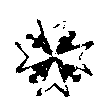
\includegraphics[width=14.726716981132075pt]{authority_rosette_native_supported_mask.png}}}}
\providecommand{\noethpIIsrcfnmark}[1]{\begingroup\renewcommand{\thefootnote}{#1}\footnotemark\addtocounter{footnote}{-1}\endgroup}
\providecommand{\noethpIIsrcfntext}[2]{\begingroup\renewcommand{\thefootnote}{#1}\footnotetext{#2}\endgroup}
\providecommand{\foreign}[1]{#1}
\begin{document}


\clearpage
\begingroup
\setcounter{footnote}{0}
% BEGIN PRODUCER UNIT 001
% Source: ../../../../noether/02_slavic_working_corpus/translations/paper01/interslavic/v001/Noether_Paper01_Interslavic_v001.tex
% Identity: 7284 B / SHA-256 94B7533CFA0F30F0197FA9622C7289A4AA563999FFDDA9D10C479866D7F4F478
\setlength{\parindent}{1.25em}
\setlength{\parskip}{0pt}
\emergencystretch=4em
% BEGIN UNIT BODY
\begin{center}
{\Large\bfseries 1. Конструкција система форм за тернарну\\ форму четвртого степена}\par
\vspace{1.5em}
Sitzungsberichte Физикално-медицинского дружства в Ерлангену 39 (1907), с. 176--179
\end{center}

\vspace{4em}
\begin{center}
(Извод из дисертације авторкы.)
\end{center}

Систем форм тернарној биквадратичној формы, то јест тернарној формы четвртого степена, изследовали Гордан, Маисано и Пасцал.\footnote{P. Gordan, \emph{\foreign{Über das volle Formensystem der ternären biquadratischen Form}} $f=x_1^3x_2+x_2^3x_3+x_3^3x_1$ (Math. Annalen, том XVII, с. 217--233, 1880); G. Maisano, 1. \emph{\foreign{Sistemi completi dei primi cinque gradi della forma ternaria biquadratica e degl' invarianti, covarianti e contravarianti di sesto grado}} (Гиорн. di Баттаглини XIX). 2. \emph{\foreign{Sui covarianti indipendenti di $6^\circ$ grado nei coefficienti della forma biquadratica ternaria}} (Rend. Circ. Мат. di Палермо И, 1887); E. Pascal, \emph{\foreign{Contributo alla teoria della forma ternaria biquadratica e delle sue varie decomposizioni in fattori}} (Мемориа премиата далла Р. Аццадемиа delle сциензе фисицхе е математицхе di Наполи, 1905).}
Гордан конструује полны систем форм, состављен из 54 конструкциј, за специалну автоморфну форму
\[
f=x_1^3x_2+x_2^3x_3+x_3^3x_1,
\]
на основє подобных принципов, кторе он дал за системы форм в бинарној области.

У Маисана за обчу биквадратичну форму конструоване сут формы до петого реда вкључитељно,\footnote{Под "редом" туто разумєје се степењ в коефициентах, а под "степенем" степењ в прємєнных.}
а такоже нєкторе инварианты, коварианты и контраварианты вышего реда. On слєдује методє, ктору Гордан примєнил в првом тому \emph{Mathematische Annalen} за тернарну кубичну форму. Пасцал, користајучи резултатами Маисана, главно се занима пытањем, когда биквадратична форма разкладаје се на факторы.\footnote{В својој другој краткој нотє Маисано пробује доказати линеарну зависимост трєх ковариантов реда 6 и степена 6. Насупрот тому не вполнє законченому доказу Пасцал мни, же је доказал линеарну независимост тыцх трєх ковариантов реда 6, а такоже трєх инвариантов реда 9. Но в току мојих рачунениј показало се, же линеарно одношење в истинє обстаје и меджу трєми ковариантами, и меджу трєми инвариантами. В означењу Пасцала једнозначне формулы сут:
\[
0=20\Omega_1+6\Omega_2-3\Omega_3+4fC_1-12fC_2-4A\cdot\Delta,
\]
\[
0=4A^3-15AB+30C-90D+9E.
\]}

\textbf{Циљ мојих изслєдованиј јест конструкција система форм за обчу тернарну форму четвртого степена. Најпрво дајут се само главне основы и конструује се так называны "односно полны систем".\footnote{За термин срав. Гордан--Керсцхенстеинер, \emph{\foreign{Vorlesungen über Invariantentheorie}}, том II, с. 227.}}

Основна мысљ при конструкцији системов тернарных форм јест така сама како в бинарној области. Починајучи од првого односно полного система, то јест од система форм, прєнесеных из бинарного случаја, по опрєдєљеном закону прєходи се к системам с все вышим модулом. То иде дотуд, докуд систем нєкојего модула, ако сам модул взети за основну форму, не стане конечным и познаным, или докуд модул не можно снижити к формам, кторе имајут инвариант како фактор. В првом случају абсолутно полны систем настаје трансвекцијеју односно полного система со системом модула; в другом случају односно полны и абсолутно полны систем сут идентични. Из обчего Хилбертового доказа конечности системов форм слєдује, же та процедура мора дојти до конца.

В нашем случају модул $(abc)$ првого односно полного система можно свести к модулам
\[
\Delta=(abc)^2a_x^2b_x^2c_x^2\quad\text{и}\quad \nu=(abu)^4;
\]
из тога лахко добываје се односно полны систем модуло $\nu$. Како ред модулов выбира се нынє формы
\[
\nu;\qquad \nu^{(\nu)}=(\nu\nu_1x)^4=s_x^4,
\]
\[
\nu^{(s)}=(ss'u)^4\ldots
\]
и како даљше модулы придајут се двє квадратичне формы, кторе наставајут при конструкцији односно полного система модуло $s$, именно $u_\sigma^2$ и $t_x^2$. Потом можно показати, же модул слєдујучи по $s$, именно $(ss'u)^4$, јест редуцибилны к модулу $(\varrho,t)$. Но симултанны систем двух квадратичных форм јест конечны и познаны; тым досегнуты јест выше означены конец. Односно полны систем модуло $(\varrho,t)$ даје 331 конструкциј. ---

Додам јешче нєколико указаниј о примєњеној методє.

Основны процес творјења форм, процес контракције, в тернарној области можно опрєдєлити так.

Ако в симболичном продукту
\[
s_x^m t_x^n u_\sigma^\mu u_\tau^\nu
\]
замєнити пары факторов
\[
\begin{array}{c|c|c|c|c}
 & s_xt_x & u_\sigma u_\tau & s_xu_\sigma\ \text{или}\ s_xu_\tau & t_xu_\tau\ \text{или}\ t_xu_\sigma\\
\text{одношно с} & (stu) & (\sigma\tau x) & s_\sigma\ \text{или}\ s_\tau & t_\tau\ \text{или}\ t_\sigma\\
\text{контракција} & \mathrm{I} & \mathrm{II} & \mathrm{III} & \mathrm{IV}
\end{array}
\]
тогда наставајуче формы сут добјене из почетковој формы контракцијам.\footnote{Гордан, Math. Annalen, том XVII, с. 219.}

При том можно все јешче положити $s_\sigma=0$ и $t_\tau=0$. За взајемну свез меджу поједиными контракцијами имаје мєсто слєдујуча теорема.

\textbf{Контракције I и II сут основне контракције. Из њих, независно од пореда складања, можно составити контракције III и IV. Другыми словами: да бы се створили все формы, кторе наставајут из даного израза контракцијам, достаточно јест примєњати само контракције I и II.}\footnote{Теорема има изкључење в случају, когда $n$ и $\mu$, одношно $m$ и $\nu$, једночасно исчезајут; тогда ред форм снижаје се к диагоналному члену.}

Под "редом форм" разумєјемо почетну форму заједно со всими формами, кторе из њеј наставајут повторным контракцијам самеј со собоју. По теореми ред форм
\[
s_x^m t_x^n u_\sigma^\mu u_\tau^\nu
\]
можно размєстити в премоуголној схемє. При идењу в тој схемє добываје се:
\begin{enumerate}
\item једну колону на право -- все формы, кторе наставајут из сусєдных форм контракцијам И;
\item једен ред в низ -- все формы, кторе наставајут из форм над ними контракцијам II.
\end{enumerate}
Так добывајут се все формы, кторе наставајут контракцијам.

Под тыми прєдположењами теоремы о редуцентах можно изректи в најобчејшеј формє, под опрєдєљењем
\begin{center}
\textbf{редуцент јест редуцибилны ред форм.}
\end{center}
Обча редукцијска теорема потом гласи:

\begin{center}
\textbf{Ако почетна форма реда форм јест редуцибилна зато, же једен из јеј членов настал контракцијам с редуцентом, и ако конечна форма тога реда настала јест из того самого члена контракцијам, тогда цєлы ред форм јест редуцибилны.}
\end{center}

Како даљше методы редукције трєба назвати:
\begin{enumerate}
\item так называну двојну редукцију, то јест редукцију једној формы двома способами, да бы се добило одношење меджу вышими формами;
\item контракција с формами, кторе разкладајут се на факторы; та метода честично има характер редукције с помочју редуцентов, а честично характер двојној редукције.
\end{enumerate}
% END UNIT BODY
% END PRODUCER UNIT 001
\endgroup


\clearpage
\begingroup
\setcounter{footnote}{0}
% BEGIN PRODUCER UNIT 002
% Source: ../../../../noether/02_slavic_working_corpus/translations/paper02/interslavic/v001/Noether_Paper02_Introduction_Interslavic_v001.tex
% Identity: 6814 B / SHA-256 D4EBD958552D375AACD91F5E92941B0FD98E34B1992B16EAB5FD953AD0946C7C
\setlength{\parindent}{1.25em}
\setlength{\parskip}{0pt}
\emergencystretch=4em
% BEGIN UNIT BODY
\begin{center}
{\Large\bfseries 2. Конструкција система форм за тернарну\\ биквадратичну форму}\par
\vspace{1.5em}
\emph{\foreign{Journal für die reine und angewandte Mathematik}} 134 (1908), с. 23--90 и двє табелы
\end{center}

\vspace{3em}

\begin{center}
\textbf{Ввод.}
\end{center}

Систем форм тернарној биквадратичној формы изслєдовали Гордан, Маисано и Пасцал.\footnote{Краткы извод из ввода и главы И појавил се в \emph{\foreign{Sitzungsberichte der physikalisch-medizinischen Sozietät Erlangen 1907}}, с. 176--179.}\footnote{P. Gordan, \emph{\foreign{Über das volle Formensystem der ternären biquadratischen Form}}
\[
f=x_1^3x_2+x_2^3x_3+x_3^3x_1.
\]
(\emph{Math. Annalen}, том XVII (1880), с. 217--233.)
G. Maisano, 1) \emph{\foreign{Sistemi completi dei primi cinque gradi della forma ternaria biquadratica e degl' invarianti, covarianti e contravarianti di sesto grado}}. (Гиорн. di Баттаглини XIX.)
2) \emph{\foreign{Sui covarianti indipendenti di $6^\circ$ grado nei coefficienti della forma biquadratica ternaria}}. (Rend. Circ. Мат. di Палермо И, 1887.)
E. Pascal, \emph{\foreign{Contributo alla teoria della forma ternaria biquadratica e delle sue varie decomposizioni in fattori}}. (Мемориа премиата далла Р. Аццадемиа delle сциензе фисицхе е математицхе di Наполи. 1905.)}
Гордан конструује полны систем форм, составјены из 54 конструкциј, за специалну автоморфну форму
\[
f=x_1^3x_2+x_2^3x_3+x_3^3x_1,
\]
на основє подобных принципов, кторе он дал за системы форм в бинарној области.

У Маисана за обчу биквадратичну форму конструоване сут все формы до петого реда укључитељно,\footnote{Под "редом" туто разумєје се степењ в коефициентах, а под "степенем" степењ в прємєнных.}
а такоже нєкторе инварианты, коварианты и контраварианты вышего реда. On користаје методу, ктору Гордан примєнил в првом тому \emph{Mathematische Annalen} к тернарној кубичној формє. Пасцал, опирајучи се на резултаты Маисана, главно се занима пытањем разклада биквадратичној формы на факторы.\footnote{В својој другој краткој нотє Маисано пробује доказати линеарну зависимост трєх ковариантов реда 6 и степена 6. Насупрот тому не вполнє доконченому доказу Пасцал мни, же доказал линеарну независимост тыцх трєх ковариантов реда 6, а такоже трєх инвариантов реда 9. Но то, же линеарно одношење в истинє обстаје меджу трєми ковариантами, с једној страны, и трєми инвариантами, с другој страны, показујут формулы (13), § 11, и (22), примєтка к § 17, тутој работы, кде та одношења сут дана једнозначно. По информацији Пасцала противорєчје објасњаје се числовој погрєшкоју в изразу јего контраварианта $p$ (туто означеного $\varrho$), с. 46 јего статји.}

{\itshape Циљ слєдујучих изслєдованиј јест конструкција система форм за обчу тернарну биквадратичну форму. В тој работє дајут се само главне основы и конструује се так называны "односно полны систем".\footnote{За термин гледати § 3а.}}

Работа тєсно примыкаје к работє Гордана; но принципы, кторе там были дане само в обчем виду, трєба было најпрво изработати в подробностјах. С помочју теоремы о свези меджу контракцијами и прєз введење "реда форм" (§ 1) редукцијске теоремы формулујут се точно и доплњајут се (§ 3), доколє рекурсивна конструкција специалных развитиј в реды (§ 2) даје рачунно средство за стварно проведење редукциј.

Основна мысљ конструкције системов тернарных форм јест така сама како в бинарној области. Починајучи од првого односно полного система --- система форм прєнесеных из бинарного случаја, --- по опрєдєљеном закону прєходи се к системам с все вышим модулом. Та поступност иде дотуд, докуд систем нєкојего модула, ако сам модул взети за основну форму, не стане конечным и познаным, или докуд модул не можно свести к формам, кторе имајут инварианты како факторы. В првом случају абсолутно полны систем настаје трансвекцијеју односно полного система со системом модула; в другом случају односно полны и абсолутно полны систем сут идентичне. Из обчего Хилбертового доказа конечности системов форм слєдује, же та процедура мора дојти до конца.

В нашем случају модул $(abc)$ првого односно полного система (§ 4) своди се к модулам
\[
\Delta=(abc)^2a_x^2b_x^2c_x^2\quad\text{и}\quad \nu=(abu)^4
\]
(§ 5), а потом находи се односно полны систем модуло $\nu$ (§ 6). Ты резултаты сут уж дане в работє Гордана за обчу биквадратичну форму; наш способ извода једнак лехче прєноси се на формы вышего степена.

Како ред модулов нынє выбирајемо формы (§ 7):
\[
\nu,\qquad \nu(\nu)=(\nu\nu_1x)^4=s_x^4,\qquad \nu(s)=(ss'u)^4,\ldots .
\]

При конструкцији односно полного система модуло $s$ двє квадратичне формы, наставајуче в систему, $u_\varrho^2$ и $t_x^2$, придајут се како модулы (§§ 9 и 10), и одтуд конструује се односно полны систем модуло $(s,\varrho,t)$. Потом показује се (§ 17), же модул $(ss'u)^4$ јест редуцибилны к модулам $\varrho$ и $t$. Прєз то слєдујучи выши систем прєходи в односно полны систем модуло $(\varrho,t)$. Но симултанны систем двух квадратичных форм јест конечны и познаны, а в обчем случају составјен јест из 20 конструкциј;\footnote{Срав. Цлебсцх--Линдеманн, \emph{\foreign{Vorlesungen über Geometrie}} (том I, с. 288 и даље), систем двух когредиентных форм. Гордан, \emph{\foreign{Über Büschel von Kegelschnitten}} (\emph{Math. Ann.}, том XIX, с. 530), систем двух контрагредиентных форм.}
тым с конструкцијеју односно полного система модуло $(\varrho,t)$ досегнуты јест выше означены конец. Трансвекција того система со системом $(\varrho,t)$ за конструкцију абсолутно полного система остаје задржана за позднєјши час.

Како односно полны систем модуло $(\varrho,t)$ најдене сут 331 конструкције; в прилагајенеј табели оне сут упоредковане по степену в прємєнных $x$ и $u$.

На концу дајемо преглед введеных симболов:
\begin{align*}
f&=a_x^4,\\
\theta&=\theta_x^4u_\vartheta^2=(abu)^2a_x^2b_x^2,\\
K&=K_x^6u_k^3=(a\theta u)u_\vartheta^2a_x^3\theta_x^3,\\
j&=u_j^6=(a\theta u)^4u_\vartheta^2,\\
\Delta&=\Delta_x^6=a_\vartheta^2a_x^2\theta_x^4=(abc)^2a_x^2b_x^2c_x^2,\\
N&=N_x^8u_\eta=(a\Delta u)a_x^3\Delta_x^5,\\
\nu&=u_\nu^4=(abu)^4,\\
H&=H_x^2u_\eta^4=(\nu\nu_1x)^2u_\nu^2u_{\nu_1}^2,\\
L&=L_x^3u_l^6=(\nu\eta x)H_x^2u_\nu^3u_\eta^3,\\
g&=g_x^6=(\nu\eta x)^4H_x^2,\\
\sigma&=u_\sigma^6=H_\nu^2u_\nu^2u_\eta^4,\\
s&=s_x^4=(\nu\nu_1x)^4,\\
Z&=Z_x^4u_\zeta^2=(ss'u)^2s_x^2s_x'^2,\\
\varrho&=u_\varrho^2=\theta_\nu^4u_\vartheta^2,\\
t&=t_x^2=a_\eta^4H_x^2,\\
i&=a_\nu^4,\\
J&=s_\nu^4.
\end{align*}
% END UNIT BODY
% END PRODUCER UNIT 002
\endgroup


\clearpage
\begingroup
\setcounter{footnote}{0}
% BEGIN PRODUCER UNIT 003
% Source: ../producer_units/Noether_Paper02_Section01_Interslavic_v001.tex
% Identity: 7674 B / SHA-256 594F093A49D5FF186EA9126E0757B635F45EA2ED8391FAC1AD117D3308033998
\setlength{\parindent}{1.25em}
\setlength{\parskip}{0pt}
\emergencystretch=4em
% BEGIN UNIT BODY
\begin{center}
{\Large\bfseries Глава I. \quad Обче теоремы о тернарных формах.}
\end{center}

\begin{center}
\textbf{§ 1. \quad Процес контракције. \quad Реды форм.}
\end{center}

Основны процес творјења форм јест процес контракције, кторы в тернарној области можно опрєдєлити слєдујучим способом. Нехај буде даны симболичны продукт
\[
s_x^m t_x^n u_\sigma^\mu u_\tau^\nu .
\]
Ако пары факторов
\[
s_xt_x\qquad u_\sigma u_\tau\qquad s_xu_\sigma\ \text{или}\ s_xu_\tau
\qquad t_xu_\tau\ \text{или}\ t_xu_\sigma
\]
замєнити одношно с
\[
(stu)\qquad (\sigma\tau x)\qquad s_\sigma\ \text{или}\ s_\tau
\qquad t_\tau\ \text{или}\ t_\sigma,
\]
то јест со контракцијами
\[
\text{И}\qquad\text{II}\qquad\text{III}\qquad\text{IV},
\]
тогда наставајуче формы наставајут из почетковој формы прєз контракцију.\footnote{Гордан, \emph{Math. Annalen}, том XVII, с. 219.}

При том израз $s_x^m t_x^n u_\sigma^\mu u_\tau^\nu$ можно разумєти или како стварны продукт двух форм $S\cdot T$, или како једину форму с нєколико редами симболов:
\[
s_x^m t_x^n u_\sigma^\mu u_\tau^\nu=A_x^{m+n}u_x^{\mu+\nu}.
\]
В првом случају говоримо о контракцији формы $S$ с формоју $T$, в другом случају о «контракцији формы $A$ самеј со собоју». Дља краткости в слєдујучем всегда прєдпокладамо (то в истинє јест случај при всих позднєје разгледаных формах), же
\[
\tag{a}
s_\sigma^\lambda=0,\qquad t_\tau^\chi=0
\]
за всаке $\lambda$ и $\chi$, различне од нуле, и заједно с какымиколи другыми контракцијами. То говори, же форма $s_x^m t_y^n u_\sigma^\mu u_\tau^\nu$ јест так называна «нормална форма», то јест при примєњењу $\Omega$-процеса она исчезаје и по прємєнных $x$ и $u$, и по прємєнных $y$ и $v$.

Условје (а) зато не јест ограничење; јего можно всегда досегнути.\footnote{Срав. Гордан, \emph{Math. Annalen}, том V, с. 104.}

За свез меджу поједиными контракцијами имаје мєсто слєдујуча теорема:

{\itshape Теорема I. Контракције I и II сут основне контракције; из њих, независно од пореда складања, можно составити контракције III и IV. Другыми словами: да бы се створили все формы наставајуче из даного израза прєз контракцију, трєба примєњати само контракције I и II.}

Доказ. По теоремє идентичности, одношно по теоремє продукта за матрице, с увагој на (а) добывајемо
\[
(\widehat{st}\sigma x)=-t_\sigma,\qquad
(\widehat{\sigma\tau}su)=-s_\tau,
\]
\[
(\widehat{st}\tau x)=s_\tau,\qquad
(\widehat{\sigma\tau}tu)=t_\sigma,
\]
\[
(stu)(\sigma\tau x)=s_\tau+t_\sigma-u_x\,s_\tau t_\sigma .
\]
Зато прєз складање контракциј I и II наставајут контракције III и IV; то јест такоже при примєњењу контракције II к контракцији И, то јест к факторам $(stu)u_\sigma u_\tau$, како и при примєњењу контракције И к контракцији II, то јест к факторам $(\sigma\tau x)s_xt_x$.

Под {\itshape редом форм}\footnote{Срав. Цлебсцх, \emph{\foreign{Über eine Fundamentalaufgabe der Invariantentheorie}} (\foreign{Abh. der Gött. Ges. d. Wiss.}, том XVII): § 17 и конец § 18. «Ред форм» разликује се од тамо введеного «властно редуцираного еквивалентного система» принципом упоредковања по вышших формах.}
разумєјемо почетну форму заједно со всими формами, кторе из њеј настали сут контракцијам самеј со собоју, и означујемо ред форм почетноју формоју. «Выша форма» туто значи всаку форму с боље многым контракцијам самеј со собоју; меджу равноправными контракцијами $s_\tau$ и $t_\sigma$ једно мора быти нормовано како выше. По закону творјења реда форм слєдује:

1) Всака форма реда форм јест линеарна в симболах почетној формы.

2) Ред форм јест једнозначно опрєдєљен за почетне формы с по двєма редами контрагредиентных симболов; при почетных формах с боље редами симболов јего трєба једнозначно нормовати вызначењем специалных контракциј меджу тыми, кторе сут свезане теоремоју идентичности.

По теоремє И ред форм $s_x^m t_x^n u_\sigma^\mu u_\tau^\nu$ ($m>n;\ \mu>\nu$) можно размєстити по слєдујучеј премоуголној схемє:
\begingroup\small
\[
\begin{array}{c|c|c|c|c}
s_x^m t_x^n u_\sigma^\mu u_\tau^\nu
& (stu)
& (stu)^2
& \cdots
& \noethpIIrosette\\[0.3em]
(\sigma\tau x)
& t_\sigma,\ s_\tau
& t_\sigma(stu),\ s_\tau(stu)
& \cdots
& \vdots\\[0.3em]
(\sigma\tau x)^2
& t_\sigma(\sigma\tau x),\ s_\tau(\sigma\tau x)
& t_\sigma^2,\ t_\sigma s_\tau,\ s_\tau^2
& \cdots
& \vdots\\[0.3em]
\vdots&\vdots&\vdots&\ddots&\vdots\\[0.3em]
(\sigma\tau x)^\nu
& t_\sigma(\sigma\tau x)^{\nu-1},\ s_\tau(\sigma\tau x)^{\nu-1}
& t_\sigma^2(\sigma\tau x)^{\nu-2},\ t_\sigma s_\tau(\sigma\tau x)^{\nu-2},\ s_\tau^2(\sigma\tau x)^{\nu-2}
& \cdots
& \vdots\\[0.3em]
\vdots
& t_\sigma(\sigma\tau x)^\nu
& t_\sigma^2(\sigma\tau x)^{\nu-1},\ t_\sigma s_\tau(\sigma\tau x)^{\nu-1}
& \cdots
& \vdots\\[0.3em]
\vdots
& \vdots
& t_\sigma^2(\sigma\tau x)^\nu
& \cdots
& \vdots
\end{array}
\]
\endgroup
и одношно продолжену нижњу чест
\begingroup\small
\[
\begin{array}{r@{\quad}c}
\noethpIIrosette\noethpIIsrcfnmark{*)}
&
\begin{array}{c|c|c}
(stu)^n & \cdots & \cdots\\[0.3em]
t_\sigma(stu)^{n-1},\ s_\tau(stu)^{n-1}
& s_\tau(stu)^n & \cdots\\[0.3em]
t_\sigma^2(stu)^{n-2},\ t_\sigma s_\tau(stu)^{n-2},\ s_\tau^2(stu)^{n-2}
& t_\sigma s_\tau(stu)^{n-1},\ s_\tau^2(stu)^{n-1}
& s_\tau^2(stu)^n .
\end{array}
\end{array}
\]
\endgroup
\noethpIIsrcfntext{*)}{Туто, и подобно в слєдујучем, нижњу чест означену звєздочкоју трєба приложити к такоже означеному мєсту в правој горној чести схемы.}

Туто добывајемо, ако се иде

1) једну колону на право, все формы, кторе наставајут из сусєдных форм прєз контракцију И;

2) једен ред в низ, все формы, кторе наставајут из форм стојечих над ними прєз контракцију II;

и с тым все формы, кторе наставајут прєз контракцију.

Либовољна форма цєлого реда форм, $t_\sigma^\kappa s_\tau^\lambda(stu)^\mu$ или $t_\sigma^\kappa s_\tau^\lambda(\sigma\tau x)^\nu$, твори почеток нового реда форм. On состоји се из всих тыцх форм премоуголној схемы, кторе имајут форму $t_\sigma^\kappa s_\tau^\lambda(stu)^\mu$ или $t_\sigma^\kappa s_\tau^\lambda(\sigma\tau x)^\nu$ како лєвы горны кут и имајут фактор $t_\sigma^\kappa s_\tau^\lambda$.

Додатна примєтка. Теорема I има изкључење в случају, когда числа $n$ и $\mu$ (одношно $m$ и $\nu$) станут равне нули, тако же контракције I, II и IV уж не обстајајут, но контракција III (одношно IV) јешче обстаје. В том случају редом форм называјемо диагоналны член схемы:
\[
\begin{array}{ccccc}
s_x^m u_\tau^\nu &&&& t_x^n u_\sigma^\mu\\
& s_\tau && t_\sigma &\\
& s_\tau^2 && t_\sigma^2 &\\
&&\ddots&&\\
&&s_\tau^\nu && t_\sigma^\mu .
\end{array}
\]
В согласности с одсутностју контракциј I и II, развитје в ред по поларах реда форм в том случају всегда снижаје се к почетному члену; але теоремы о редуцентах оставајут в силє.
% END UNIT BODY
% END PRODUCER UNIT 003
\endgroup


\clearpage
\begingroup
\setcounter{footnote}{0}
% BEGIN PRODUCER UNIT 004
% Source: ../../../../noether/02_slavic_working_corpus/translations/paper02/interslavic/v001/Noether_Paper02_Section02_Interslavic_v001.tex
% Identity: 6938 B / SHA-256 AF6E7C4F4E44E8016C1E63C958CD3F543AF7BAC3A3F37450A1AA15635636B801
\setlength{\parindent}{1.25em}
\setlength{\parskip}{0pt}
\emergencystretch=4em
% BEGIN UNIT BODY
\begin{center}
\textbf{§ 2. \quad Развитја в ред по поларах реда форм.}
\end{center}

За формы с $n$ прємєнными експлицитно сут поставјене двє врсты развитиј в ред\footnote{Срав. Гордан, \emph{\foreign{Über Kombinanten}}, § 2 и 5 (\emph{Math. Ann.}, том V).}:

1) за формы с по једным редом контрагредиентных прємєнных, $s_x^m u_\tau^\nu$, ред, кторы иде по степењах $u_x$ и кторего коефициенты сут «нормалне формы»;

2) за формы с двєма редами когредиентных прємєнных $s_x^m t_x^n$ развитје по поларах елементарных ковариантов (поларах реда форм $s_x^m t_x^n$), кторе в тернарном случају гласи так\footnote{Срав. Студы, \emph{\foreign{Methoden zur Theorie der ternären Formen}} (Teubner 1889) II. § 7. В разликє од тамошњего вывода наш даје метод брзого рачуного опрєдєљења числовых коефициентов $C_{pr\varrho}$. Развитје Цлебсцха--Студыја при специализацији а), а') имало бы облик:
\[
(stu)^\mu u_\tau^{\nu-\kappa}v_\tau^\kappa s_x^m t_x^{\,n-\lambda}(tuv)^\lambda
=\sum_{p,r,\varrho} C_{pr\varrho}
\bigl[s_\tau^\varrho(stu)^{\mu+r-\varrho}\bigr]_{\widehat{uv}^{\lambda-r+\varrho}v^{\nu-\varrho},\,u^p,\,(vw=\widehat{xw})},
\]
и зато не допушча упрошчења, кторе в нашем развитју настаје уж в току рачуна, когда се знајет, же все члены с фактором $u_x$ трєба изпустити.}:
\[
\tag{I}
s_x^m t_x^{n-\lambda}t_y^\lambda
=\sum_{\varrho}
\frac{\binom{m}{\varrho}\binom{\lambda}{\varrho}}
{\binom{m+n-\varrho+1}{\varrho}}
\bigl[(st\widehat{xy})^\varrho s_x^{m-\varrho}t_x^{n-\varrho}\bigr]_{y^{\lambda-\varrho}}.
\]

Мы комбинујемо оба развитја тако, же за формы с по двєма редами контрагредиентных прємєнных
\[
s_x^m t_x^{n-\lambda}t_y^\lambda u_\sigma^\mu u_\tau^{\nu-\kappa}v_\tau^\kappa
\]
постављамо развитја по степењах $u_x$, кторых коефициенты сут сложене полары реда форм $s_x^m t_x^n u_\sigma^\mu u_\tau^\nu$, взете по прємєнных $x$ и $u$.

Достаточно јест поставити ред за двє контрагредиентне реды симболов (одношно прємєнных), зато же прєз сједињање всакых двух редов симболов (прємєнных) в једен новы ред можно формы с боље редами симболов (прємєнных) свести к тому случају.

Да бы се досегнуло, же все формы реда форм имајут само по два реды симболов или прємєнных, специализујемо:
\[
\begin{array}{ll}
\text{а) } \sigma=\widehat{st}, & \text{а') } y=\widehat{uv},\\[0.3em]
\text{б) } s=\widehat{\sigma\tau}, & \text{б') } v=\widehat{xy},
\end{array}
\]
и проводимо развитје за специализацију а), а').

Прємым прєносом развитја И добывајут се сложене полары за формы $(stu)^\mu s_x^m t_x^{n-\lambda}t_y^\lambda$, меджутым за формы $(stu)^\mu u_\tau^{\nu-\kappa}v_\tau^\kappa s_x^m t_x^{n-\lambda}t_y^\lambda$ вмєсто сложеных поларов наставајут члены такого рода, кторых оцєњење потрєбује введење все новых помоцных прємєнных, кторе трєба идентификовати јединоразно на концу; прєз то рачун стаје непотрєбно скомпликованы.

Зато избирајемо непрємы пут: прєдставјамо сложене полары всих форм реда форм, то јест изразы
\[
\bigl[s_\tau^\varrho(stu)^{\mu-\varrho+r}\bigr]_{y^\lambda}^{v^\kappa}
\]
прєз почетне члены тыцх поларов и, обратом наставајучего рекурсивного система равнаниј, добывајемо желано развитје по поларах.

По принципу прєноса за $\lambda$-ту полару формы $s_x^m t_x^n:[s_x^m t_x^n]_{y^\lambda}$ ($\lambda\le n$) имаје мєсто слєдујуче развитје (случај $\lambda>n$ своди се к првому прєз развитје $[s_y^m t_y^n]_{x^{m+n-\lambda}}$)\footnote{Гордан, \emph{\foreign{Die Resultante binärer Formen}} (Кап. И, § 5). Rend. Circ. Мат. di Палермо XXII. 1906.}:
\[
\bigl[s_x^m t_x^n\bigr]_{y^\lambda}
=\sum_r (-1)^r\,
\frac{\binom{m}{r}\binom{\lambda}{r}}{\binom{m+n}{r}}\,
(st\widehat{xy})^r s_x^{m-r}t_x^{n-\lambda}t_y^{\lambda-r},
\]
и одношно за $\kappa$-ту полару формы $u_\sigma^\mu u_\tau^\nu:[u_\sigma^\mu u_\tau^\nu]_{v^\kappa}$
\[
\bigl[u_\sigma^\mu u_\tau^\nu\bigr]_{v^\kappa}
=\sum_\varrho (-1)^\varrho\,
\frac{\binom{\mu}{\varrho}\binom{\kappa}{\varrho}}{\binom{\mu+\nu}{\varrho}}\,
(\sigma\tau\widehat{uv})^\varrho u_\sigma^{\mu-\varrho}u_\tau^{\nu-\kappa}v_\tau^{\kappa-\varrho}.
\]

Множењем, с введењем специализације а) и а'), слєдује
\[
\begin{aligned}
\bigl[s_x^m t_x^n(stu)^\mu u_\tau^\nu\bigr]_{\widehat{uv}^{\lambda}}^{v^\kappa}
={}&
\sum_{r,\varrho}c_{r\varrho}\,
(st\widehat{uv})^r(st\widehat{uv})^\varrho
s_x^{m-r}t_x^{n-\lambda}(tuv)^{\lambda-r}(stu)^{\mu-\varrho}
u_\tau^{\nu-\kappa}v_\tau^{\kappa-\varrho},
\end{aligned}
\]
и из того, прєз развитје по степењах $u_x$ с вызначењем првого члена ($\sum'_{r,\varrho}$ значи, же член $r=0$, $\varrho=0$ трєба изпустити) и с увагој на (а) на с. 26,
\[
\tag{II}
\begin{aligned}
&s_x^m t_x^{n-\lambda}(tuv)^\lambda(stu)^\mu u_\tau^{\nu-\kappa}v_\tau^\kappa\\
&\quad =
\bigl[s_x^m t_x^n(stu)^\mu u_\tau^\nu\bigr]_{\widehat{uv}^{\lambda}}^{v^\kappa}\\
&\qquad
-\sum_{r,\varrho}' c_{r\varrho}\,s_\tau^\varrho(stu)^{\mu-\varrho+r}
u_\tau^{\nu-\kappa}v_\tau^{\kappa-\varrho}
s_x^{m-r}t_x^{n-\lambda}(tuv)^{\lambda-r+\varrho}v_x^r\\
&\qquad
+u_x\sum_{\varrho}\sum_{r=1}^{\lambda} c_{r\varrho}\,
s_\tau^\varrho(stu)^{\mu-\varrho+r-1}(stv)
u_\tau^{\nu-\kappa}v_\tau^{\kappa-\varrho}
s_x^{m-r}t_x^{n-\lambda}(tuv)^{\lambda-r+\varrho}v_x^{r-1}\\
&\qquad
\vdots\\
&\qquad
-(-1)^\lambda u_x^\lambda\sum_\varrho c_{\lambda\varrho}\,
s_\tau^\varrho(stu)^{\mu-\varrho}(stv)^\lambda
u_\tau^{\nu-\kappa}v_\tau^{\kappa-\varrho}
s_x^{m-\lambda}t_x^{n-\lambda}(tuv)^\varrho,
\end{aligned}
\]
кде
\[
c_{r\varrho}=(-1)^{r+\varrho}\cdot
\frac{\binom{m}{r}\binom{\lambda}{r}}{\binom{m+n}{r}}\cdot
\frac{\binom{\mu}{\varrho}\binom{\kappa}{\varrho}}{\binom{\mu+\nu}{\varrho}}
\qquad
\begin{array}{l}
\text{за }\lambda\le n,\\
\kappa\le\nu.
\end{array}
\]
и одношно за остале комбинације чисел
\[\lambda,n;\kappa,\nu.\]
Израз
\[s_x^m t_x^{n-\lambda}(tuv)^\lambda(stu)^\mu u_\tau^{\nu-\kappa}v_\tau^\kappa\]
јест зато сведены к сложенеј полари и, при примєњењу идентичности
\[
(stv)u_\tau=(stu)v_\tau-s_\tau(tuv),
\]
к сумє аналогно створеных изразов, кторе одповєдајут вышим формам реда форм.

Прєз итерацију приходимо к развитју:
\[
\tag{III}
s_x^m t_x^{n-\lambda}(tuv)^\lambda(stu)^\mu u_\tau^{\nu-\kappa}v_\tau^\kappa
=
\sum_{p,r,\varrho}u_x^p\,C_{pr\varrho}\cdot
\bigl[s_\tau^\varrho(stu)^{\mu-\varrho+r}\bigr]_{\widehat{uv}^{\lambda-r+\varrho}v^{\kappa-\varrho+p},\,v_x^{r-p}}.
\]
Числове коефициенты $C_{pr\varrho}$ једнозначно и рекурсивно рачуњут се из коефициентов $c_{r\varrho}$, $c'_{r\varrho}$ система равнаниј, кторы настаје прєз итерацију (II.) (срав. примєр на с. 42). Аналогна развитја наставајут при осталых специализацијах.
% END UNIT BODY
% END PRODUCER UNIT 004
\endgroup


\clearpage
\begingroup
\setcounter{footnote}{0}
% BEGIN PRODUCER UNIT 005
% Source: ../../../../noether/02_slavic_working_corpus/translations/paper02/interslavic/v001/Noether_Paper02_Section03_Interslavic_v001.tex
% Identity: 7634 B / SHA-256 A36275222B056854F2A2488BCDF0B823A8E7DE9A24C8836456EDD48F6A84C222
\setlength{\parindent}{1.25em}
\setlength{\parskip}{0pt}
\emergencystretch=4em
% BEGIN UNIT BODY
\begin{center}
\textbf{§ 3. \quad Редукцијне теоремы.}
\end{center}

Знане теоремы о редукцији форм и системов форм трєба нынє свезати с параграфами 1 и 2; за то потрєбне сут нєкторе опрєдєљења, взете из теорије бинарных форм.

а) Како {\itshape релативно полны систем} по модулу даного реда форм означајемо систем форм с такым својством: все творјења, кторе наставајут прєз контракцију либовољного продукта тых форм, можно изразити како цєле рационалне функције форм система, до додатного члена изразов, кторе настали прєз контракцију системных форм со системом модула\footnote{Гордан--Керсцхенстеинер, \emph{\foreign{Vorlesungen über Invariantentheorie}}, том II, с. 227.}.

б) Форму называјемо {\itshape редуцибилноју}, когда ју можно изразити прєз формы, кторе имајут инварианты како факторы, или прєз «выше формы»; то јест прєз выше формы цєлого реда форм, к кторому она належи, или прєз формы, кторе содрживајут симболы модула во вышем поредку.

Теоремы о редуцентах\footnote{Гордан, \emph{Math. Annalen}, том XVII, с. 222.} можно в најобчејшој формє изректи так:

Опрєдєљење: {\itshape редуцент јест редуцибилны ред форм.}

{\itshape Теорема II. Јестли почетна форма реда форм јест редуцибилна зато, же једен из јеј членов настал прєз контракцију с редуцентом (има редуцент како фактор), и јестли конечна форма реда форм настала из того самого члена прєз контракцију, тогда цєлы ред форм јест редуцибилны}\footnote{Упрошчење, кторе настаје прєз теорему II, можно показати на слєдујучем примєру. За специалну форму $f=x_1^3x_2+x_2^3x_3+x_3^3x_1$ израз $a_y^2a_x^2u_y^2$ јест редуцент. Из того по теоремє II слєдује редукција реда форм
\[
\theta_\nu(\vartheta\nu x)\theta_x^3u_\vartheta u_\nu^2
=
a_\nu^2(abu)-a_\nu b_\nu(aba),
\]
зато же $\theta_\nu^4=a_\nu^2b_\nu^2(abu)^2$ настала из члена $a_\nu^2(abu)$ прєз контракцију. У Гордана, тамже, с. 231, насупроти тому, редукција форм
\[
\theta_\nu(\vartheta\nu x),\quad \theta_\nu(\vartheta\nu x)^2,\quad
\theta_\nu^2,\quad \theta_\nu^2(\vartheta\nu x),\quad
\theta_\nu^2(\vartheta\nu x)^2
\]
проводит се појединачно.}.

Доказ: Ред форм настаје из почетного члена прєз контракцију самого себе, то јест с једној страны прєз выше контракције с редуцентом, с другој страны прєз контракцију редуцента самого себе. В обојих случајах, по § 2, можно все формы реда форм прєдставити како полары (прєкривања) над редом форм редуцента.

Закључење од почетној формы к цєлому реду форм уж не имаје мєсто при осталых методах редукције. То сут:

1) так называна «двојна редукција».

Под тым разумєјемо редукцију израза, кторы има два меджусобно независне редуценты како факторы, двојим способом; прєз то наставајут релације меджу вышими формами, к кторым было редуцирано.

Систематичным примєњењем «двојној редукције» трєба с једној страны добити все релације\footnote{Тако сут, напримєр, прєз «двојну редукцију» најдене: редукција формы $a_\eta^4$ (§ 10), јединој формы, ктору Маисано збыточно внесл в систем; потом в примєтки к уводу споменуте релације меджу 3 ковариантами и 3 инвариантами.}; с другој страны, јестли «двојна редукција», примєњена к различным изразам, не даје новых релациј, имамо и критериј независности вышших форм и контролу рачуна.

2) {\itshape Контракција с разложимыми формами.}

Под «разложимыми формами» -- с малым обобчењем обичного појма -- разумєјемо формы, кторе можно изразити прєз продукты форм нижшего степена и прєз «выше» формы. Продукты форм при једнократној контракцији прєходет в продукты; такоже продукты нелинеарных форм при двократној контракцији при специализацијах а') и б') (§ 2) по теоремє продукта:
\[
a_yb_y a_xb_x=\frac12a_y^2b_x^2+\frac12b_y^2a_x^2-\frac12(ab\widehat{yx})^2.
\]
Прве полары (прєкривања) и нєкторе друге полары разложимых форм зато сут поновно разложиме формы. Из того слєдује:

Член једнократного (одношно двократного) прєкривања над разложимоју формоју, кторы настал прєз једнократну (одношно двократну) контракцију с разложимоју формоју, сам стаје разложима форма:

а) когда слєдујуче выше формы в реду форм разложимој формы разлагајут се или ставајут редуцибилне, или такоже когда при једнократној контракцији наставајут специализације $y=\widehat{uv}$ или $v=\widehat{xy}$;

б) когда остале једнократне контракције водет к вышим формам (срав. § 12, Б. $H_k$ и $H_k(k\eta x)$).

Таковы член прєкривања може такоже разложити се:

ц) когда остале једнократне контракције водет к нижшим формам, кторе независно од контракције с разложимоју формоју разлагајут се, то можно их изразити прєз продукты и прєз форму, ктору трєба редуцирати. При том трєба всакократно најпрво рачуном овєрјати, же числовы коефициент одговарјајучего члена не исчезаје идентично. То јест ничто друго неж «двојна редукција» нижшеј формы (срав. § 23, Ц. $H_q(\theta H u)(\theta s u)$).

Разложиме формы наставајут прєз все једнократне контракције с функционалными детерминантами\footnote{Срав. Гордан, тамже, § 3.}, кромє того прєз нєкторе выше контракције. Имамо
\[
(st\widehat{yx})s_y=\frac12\,t\,s_y^2-\frac12\,s\,t_y^2+\frac12(st\widehat{yx})^2,
\]
\[
(st\widehat{yx})^2s_y^2=\frac13\,t\,s_y^3-\frac13\,s\,t_y^3+s_y(st\widehat{yx})^2-\frac13(st\widehat{yx})^3.
\]
Аналогичне формулы имајут мєсто за дуалистичне формы
\[
(\sigma\tau\widehat{\nu u})v_\sigma
\quad\text{и}\quad
(\sigma\tau\widehat{\nu u})v_\sigma^2.
\]

Из теоремов того параграфа за поставјење всих нередуцибилных форм, кторе наставајут из контракције $S$ с $T$, добыва се слєдујуче правило:

Идємо, починајучи с најнижшими контракцијами, по либовољном напријед установјеном путу (напримєр по редах или симетрично к диагоналному члену) тако далеко в творјењу реда форм $ST$, покы не дојдемо до формы, ктора има редуцент како фактор. Ред форм опрєдєљены тоју формоју трєба изпустити, когда конечна форма изполња условје поставјено в теоремє II. Послє изкључења всих редуцибилных редов форм трєба прєз примєњење двојној редукције одстранити все остале редуцибилне, и такоже все разложиме формы. Мєста цєлого реда форм, кторе сут двојно прєкрыте независно редуцибилными редами форм, давајут повод к редукцији вышших форм (срав. § 11, Д).

\clearpage
\noindent\textbf{Теорема III.}
{\itshape Формы взете из бинарној области, то јест оне формы, кторе наставајут из системных форм одговарјајучего бинарного формы по Цлебсцховом принципу прєноса прєз обрубљење, творет релативно полны систем мод $(abc)$.}

\noindent\textbf{Доказ:}
Бинарној релацији, ктора говори, же формы $Q'_1,\ldots,Q'_n$ творет полны систем једној бинарној основној формы:
\[
Q'-F(Q')=0=\sum_\lambda\bigl\{(ab)c_x+(bc)a_x+(ca)b_x\bigr\}\varphi_\lambda^{*}
\]
прєз обрубљење одговарја тернарна релација:
\[
Q-F(Q_i)=\sum_\lambda u_x\cdot(abc)\varphi_\lambda .
\]
То јест але опрєдєљајуче равнање за релативно полны систем мод $(abc)$. За биквадратичну форму систем взетых форм состоји се из слєдујучих форм:
\[
\begin{gathered}
f=a_x^4,\qquad
\theta=\theta_x^4u_\vartheta^2=(abu)^2a_x^2b_x^2,\qquad
K=K_x^6u_k^3=(a\theta u)u_\vartheta^2a_x^3\theta_x^3,\\
j=u_j^6=(a\theta u)^4u_\vartheta^2,\qquad
\nu=u_\nu^4=(abu)^4,
\end{gathered}
\]
меджу кторыми прве четыри творет релативно полны систем мод $((abc),\nu)$.
% END UNIT BODY
% END PRODUCER UNIT 005
\endgroup


\clearpage
\begingroup
\setcounter{footnote}{0}
% BEGIN PRODUCER UNIT 006
% Source: ../../../../noether/02_slavic_working_corpus/translations/paper02/interslavic/v001/Noether_Paper02_Section05_Interslavic_v001.tex
% Identity: 7256 B / SHA-256 5A63CC75BBB84E097916A6E1002E88D439F3832CB750E8B9CB9DD31EBF3E8735
\setlength{\parindent}{1.25em}
\setlength{\parskip}{0pt}
\emergencystretch=4em
\let\A\relax
\newcommand{\A}{\mathfrak A}
% BEGIN UNIT BODY
\begin{center}
\textbf{§ 5. \quad Сведење модула $(abc)$ к модулам $\A$ и $\nu$.}
\end{center}

Модул $(abc)$, даны само једным скобковым фактором, в согласју с опрєдєљењем (§ 3, а) трєба свести к формам система. Другыми словами: ред форм $(abc)$ трєба једнозначно нормовати (срав. § 1).

\[
a_s^2a_xu_x=\frac13 a_s^3u_x=\frac13 S\cdot u_x. \tag{2}
\]
\[
\left.
\begin{aligned}
(a\A u)^2&=a_s-\frac{S}{6}u_x^2,\\
(a\A u)^3&=0.
\end{aligned}
\right\} \tag{3}
\]
\[
\left.
\begin{aligned}
\theta(s)=(ss,x)^2&=2a_t+\frac13 S\cdot\theta-\frac13 Tu_x^2,\\
\theta(t)=(tt,x)^2&=-\frac13 S\cdot a_t+\frac23 T\cdot a_s+\frac1{18}S^2\cdot\theta-\frac1{18}u_x^2\cdot S\cdot T.
\end{aligned}
\right\} \tag{4}
\]

Ред модулов: $(abc)$; $\A$; $s$; $t$ (систем модула $t$ состоји се из јединој формы $t$).\footnote{Гордан--Керсцхенстеинер, тамже, с. 134.}

Покаже се, же формы
\[
\A=(abc)^2a_x^2b_x^2c_x^2,\qquad \nu=(abu)^4
\]
достаточне сут како модул, то јест же формы
\[
\begin{gathered}
\A=(abc)^2a_x^2b_x^2c_x^2,\qquad
a_\nu=(abc)(bcu)^3a_x^3,\\
a_\nu^2=(abc)^2(bcu)^2u_x^2,\qquad
i=a_\nu^4=(abc)^4
\end{gathered}
\]
опрєдєљајут ред форм $(abc)$. В реду форм $a_\nu$ не имаје формы $a_\nu^3$ по идентичности
\[
a_\nu^3=(abc)^3a_x(bcu)=\frac13 u_x\cdot(abc)^4=\frac13 i\cdot u_x.
\]

За сведење модула к вышему модулу трєба по опрєдєљењу свести најобчејше контракције, или такоже все специалне разгледане контракције с модулом, к контракцијам с вышим модулом.

Најобчејше контракције наставајут в нашем случају из изразов
\[
(abc)a_x^3b_y^3c_z^3,\qquad
(abc)a_x^2b_y^2c_z^2a_zb_xc_x
\]
(взетых из кубичных форм),
\[
(abc)a_xb_yc_za_x^2b_x^2c_x^2
\]
(взетого из квадратичных форм) и прєз поларизацију тых изразов.

За израчунање тых изразов прєз полары $\A$ и реда форм $a_\nu$, одношно прєз их почетне члены, избирајемо, како в § 2, непрємы пут. Развијамо поларны члены
\[
(abc)^2a_x^2b_y^2c_z^2,\qquad
a_\nu(\nu xy)(\nu yz)(\nu zx)a_xa_ya_z
=(abc)(bc\widehat{x}u)(bc\widehat{y}z)(bc\widehat{z}x)a_xa_ya_z\quad\text{и т. д.}
\]
како линеарне комбинације изразов со симболичным фактором $(abc)$ и, обратом система равнаниј, добывајемо искане релације, такоже релацију меджу поларами взетыми по различным комбинацијам прємєнных. За оцєњење служет теорема идентичности и теорема продукта за детерминанты.

Систем равнаниј за $(abc)a_x^3b_y^3c_z^3$ гласи:
\begingroup\small
\[
\begin{aligned}
1)\quad
\sum_3 a_\nu(\nu yz)^3a_x^3
&=6(abc)a_x^3b_y^3c_z^3
-6\sum_3(abc)a_x^3b_y^2b_zc_z^2c_y^{*},\\[0.4em]
2)\quad
3(abc)^2a_x^2b_y^2c_z^2\cdot(xyz)
-\frac12\sum_3 a_\nu^2(\nu yz)^2\nu_x^2(xyz)
&=2\sum_3(abc)a_x^3b_y^2b_zc_z^2c_y\\
&\quad-4\sum_3(abc)a_xa_ya_zb_y^2b_zc_z^2c_x,\\[0.4em]
3)\quad
a_\nu(\nu xy)(\nu yz)(\nu zx)a_xa_ya_z
&=2\sum_3(abc)a_xa_ya_zb_y^2b_zc_z^2c_x,\\[0.4em]
4)\quad
\sum_3 a_\nu(\nu yz)^3u_x^3
-\frac32\sum_3 a_\nu^2(\nu yz)^2\nu_x^2(xyz)
+\frac16 i\cdot(xyz)^3
&=6\sum_3(abc)a_xa_ya_zb_y^2b_zc_z^2c_x.
\end{aligned}
\]
\endgroup

Из того слєдује за
\[
(abc)a_x^3b_y^3c_z^3,
\]
и прєз аналогны рачун за
\[
(abc)a_x^2b_y^2c_z^2a_zb_xc_x,\qquad
(abc)a_xb_yc_za_z^2b_x^2c_x^2:
\]
\begingroup\small
\[
\begin{aligned}
(abc)a_x^3b_y^3c_z^3
&=\frac32(abc)^2a_x^2b_y^2c_z^2(xyz)
+\frac32 a_\nu(\nu xy)(\nu yz)(\nu zx)a_xa_ya_z\\
&\quad-\frac1{12}i\cdot(xyz)^3,\\[0.4em]
(\text{IV.})\quad
(abc)a_x^2b_y^2c_z^2a_zb_xc_x
&=\frac23(abc)^2a_x^2b_y^2c_z^2c_x\cdot(xyz)\\
&\quad+\frac13a_\nu(\nu xy)(\nu yz)(\nu zx)a_x^3
-\frac16 a_\nu^2(\nu xy)(\nu zx)a_x^2\cdot(xyz),\\[0.4em]
(abc)a_xb_yc_za_z^2b_x^2c_x^2
&=\frac16(abc)^2a_x^2b_z^2c_z^2\cdot(xyz).
\end{aligned}
\]
\endgroup

Тако смы добили релативно полны систем мод $(\A,\nu)$, состојечи се из четырјех форм: $f,\theta,K,j$. Из того слєдује: все прєкривања $f$ над $\theta$, кторе не сут взете из бинарној области, такоже како прєкривање $(a\theta u)^2$, редуцибилно в бинарном на $(ab)^4$, можно изразити прєз симболы $\A$ и $\nu$.\footnote{$\sum_3$ односи се к сумє над трєми членами, кторе наставајут из почетного члена прєз цикличну замєну прємєнных. Равнања имајут мєсто такоже појединачно за всакы член сумы.}

За слєдујуче фундаменталне редукцијне формулы, прєз специализацију развитја IV или краче прєз прємы рачун (замєну симболов), добывајемо за $a_\vartheta(a\theta u)^2$, $a_\vartheta^2(a\theta u)^2$, $(a\theta u)^2$ по слєдујучих почетковых формулах:
\[
\begin{aligned}
a_\vartheta(a\theta u)^2
&=(abc)(bcu)(abu)^2-\frac13(abc)(bcu)\{(bcu)a_x-u_x(abc)\}^2,\\
a_\vartheta^2(a\theta u)^2
&=(abc)^2(abu)^2-\frac13(abc)^2\{(bcu)a_x-u_x(abc)\}^2,
\end{aligned}
\]
за $((a\theta u)^2)^{*}$:
\[
\begin{aligned}
(abu)a_y^3b_x^3&=\frac32u_\vartheta(\vartheta yx)\theta_y^2+\frac14(\nu yx)^3,\\
((abu)(acu))b_x^3&=\frac32u_\vartheta(\vartheta\widehat{a}ux)(\theta au)^2+\frac14(\nu\widehat{a}ux)^3.
\end{aligned}
\]
\begingroup\small
\[
\left.
\begin{aligned}
(a\theta u)^2&=\frac16\nu\cdot f-\frac23u_x\cdot a_\nu
+\frac23u_x^2\cdot a_\nu^2-\frac{i}{18}u_x^4,\\
a_\vartheta&=\frac13u_x\cdot\A,\\
a_\vartheta(a\theta u)&=0,\\
a_\vartheta^2&=\A,\\
(a\theta u)^3&=0,\\
a_\vartheta(a\theta u)^2&=-\frac56a_\nu+\frac76u_x\cdot a_\nu^2-\frac{i}{9}u_x^3,\\
a_\vartheta^2(a\theta u)&=0,\\
(a\theta u)^4&=j,\\
a_\vartheta(a\theta u)^3&=0,\\
a_\vartheta^2(a\theta u)^2&=\frac23a_\nu^2-\frac{i}{9}u_x^2.
\end{aligned}
\right\} \tag{1}
\]
\endgroup

К тому беремо формулу, ктора такоже настала из редукције модула $(abc)$:
\[
a_\nu^3a_xu_\nu=\frac13 i\cdot u_x. \tag{2}
\]

{\itshape Из формул (1.) и (2.) и из аналогно створеных формул за основну форму $\nu$ изводет се все позднєјше редукцијне формулы прєз поларизацију}, изјмавши релације за разложиме формы. Из формул (1.) видимо:

Ред форм води:
\[
\begin{array}{rcl}
a_\vartheta(a\theta u)^2 &\text{к}& \text{самым симболам }\nu,\\[0.2em]
a_\vartheta &\text{к}& \text{симболам }\A\text{ и }\nu,\\[0.2em]
(a\theta u)^2 &\text{к}& \text{симболам }j,\A\text{ и }\nu,\\[0.2em]
(a\theta u)^2\text{ при контракцији И} &\text{к}& \text{симболам }j\text{ и }\nu,\\[0.2em]
(a\theta u)^2\text{ при контракцији II} &\text{к}& \text{симболам }\A\text{ и }\nu.
\end{array}
\]

Можемо зато замєнити:
\begin{enumerate}
\item мод $(\A,\nu)$: контракције с $j$ одговарјајучими с $(a\theta u)^2$ или $(a\theta u)^3$;
\item мод $(\nu)$: контракције с $\A$ одговарјајучими с $a_\vartheta$ или $a_\vartheta(a\theta u)$ или такоже специалными с $(a\theta u)^2$ (кторе водет само к једнократној контракцији I).
\end{enumerate}
Особито:
\begingroup\small
\[
\begin{aligned}
(a\theta u)^2\theta_y^2\theta_x^2&=\frac13(jyx)^2\pmod{\nu},&
(a\theta u)^2u_y\theta_y&=-\frac16(jyx)^2\pmod{\nu},\\
(a\theta u)^2\nu_y^2&=\frac13(\A u\nu)^2\pmod{\nu},&
(a\theta u)(a\theta\nu)u_\vartheta\nu_\vartheta&=-\frac16(\A u\nu)^2\pmod{\nu},\\
(a\theta u)^2u_\nu^2\vartheta_\nu^2&=\frac13(\A u\nu)^2\A_\nu\pmod{\nu}.
\end{aligned}
\]
\endgroup
% END UNIT BODY
% END PRODUCER UNIT 006
\endgroup


\clearpage
\begingroup
\setcounter{footnote}{0}
% BEGIN PRODUCER UNIT 007
% Source: ../../../../noether/02_slavic_working_corpus/translations/paper02/interslavic/v001/Noether_Paper02_Section06_Interslavic_v001.tex
% Identity: 9335 B / SHA-256 42FA23A1D8C0B5DA4F173A86B7932FAD7D3CEE65C78FAF5DC6296EFA8759DC0F
\setlength{\parindent}{1.25em}
\setlength{\parskip}{0pt}
\emergencystretch=4em
\allowdisplaybreaks
\let\A\relax
\newcommand{\A}{\mathfrak A}
% BEGIN UNIT BODY
\begin{center}
\textbf{§ 6. \quad Сведење модула $(\A,\nu)$ к модулу $(\nu)$.}
\end{center}

Редукцијне формулы послєдњего параграфа дајут нам срєдство непосрєдно поставити релативно полны систем мод $\nu$; увидимо, же к систему взетых форм трєба додати само формы $\A$ и $(a\A u)=N$ (аналогно како при кубичној формє и обче како обче правило).

За редукцију модула $\A$ разгледамо все специалне контракције, кторе ту входет в разглед, то јест контракције релативно полного система мод $(\A,\nu)$ со системом $\A$, и идемо од најнижших по коефициентах форм, именно од контракциј $f$ с $\A$.

За редукцију форм $(a\A u)^2$, $(a\A u)^3$, $(a\A u)^4$ замєњамо по § 5 симболы $\A$ нижшими формами реда форм, то јест развијамо изразы
\[
a_\vartheta b_\vartheta(b\theta u)^2,\qquad
a_\vartheta(a\theta u)b_\vartheta(b\theta u)^2,\qquad
a_\vartheta(a\theta u)b_\vartheta(b\theta u)^3
\]
1) по поларах реда форм $a_\vartheta$ (симболы $\A$ и $\nu$),

2) по поларах реда форм $b_\vartheta(b\theta u)^2$ (симболы $\nu$)

и добывајемо редукцијне формулы (рачун гл. ниже):
\begin{align}
\mathrm{a)}\quad (a\A u)^2
&=\frac12(\vartheta\nu x)^2-\frac25 f\cdot a_\nu^2
-\frac45u_x\cdot\theta_\nu(\vartheta\nu x)^2 \notag\\
&\quad+u_x^2\left\{\frac16 i\cdot f-\frac1{40}S\right\},\notag\\
\mathrm{b)}\quad (a\A u)^3
&=-\frac3{10}\theta_\nu(\vartheta\nu x),\tag{3}\\
\mathrm{c)}\quad (a\A u)^4
&=\frac{21}{10}\theta_\nu^2-\frac3{10}\Pi
-\frac65u_x\cdot\theta_\nu^3+\frac1{10}u_x^2\cdot\theta .\notag
\end{align}

(К тым самым резултатом води такоже двојна редукција изразов $a_\vartheta^2(b\theta u)^2$, $a_\vartheta^2(b\theta u)^3$, $a_\vartheta^2((a\theta u)^2(b\theta u)^2)$ и $a_\vartheta^2((a\theta u)(b\theta u))^3$ послє елиминације $a_\vartheta^2$.)

Из формул (3.) слєдује, же $(a\A u)^2$ јест редуцент в односу к модулу $\nu$. Из того добывамо:

1) Редукција система $\A$: ред форм $(\A\A' u)^2=a_\vartheta^2((a\A u)^2)$ имаје редуцент $(a\A u)^2$ како фактор.

2) Редукција система, кторы настал контракцијеју с модулом $\A$:

ред форм $(\theta\A u)^2$ имаје редуцент $(a\A u)^2$ како фактор.

За формы $(\theta\A u)$ и $\A_\vartheta$ добывамо:
\[
(a\A u)^2(abu)=(\theta\A u)-u_x\cdot\A_\vartheta(\theta\A u),
\]
\[
(a\A u)(a\A b)=-\frac12\A_\vartheta+\frac12u_x\cdot\A_\vartheta^2.
\]

Из редуцента $(\theta\A u)$ слєдује редукција система, кторы настаје контракцијеју с модулом $\A$.

\bigskip

Релативно полны систем мод $\nu$ состоји се зато из шести форм:
\[
f,\ \theta,\ K,\ j,\ \A,\ N.
\]

Како примєр развитја в ред из § 2 дајемо подробно изводжење формулы (3.)а; при позднєјших рачунах будемо непосрєдно ставити конечну формулу III. (Полары изчезајучих форм уж сут изпушчене током рачуна; прва линија даје врєдности внесене по развитју II, друга линија -- конечне врєдности најдене рекурсивно, починајучи с послєдњим равнањем система.) По развитју II слєдује:

\begingroup\scriptsize
\begin{align*}
\text{1)}\quad&m=3,\quad n=4,\quad \lambda=2,\quad \mu=0,\quad \nu=\chi=1,\\
a_\vartheta b_\vartheta(b\theta u)^2
&=[a_\vartheta]_{b^2}b+\frac67\{a_\vartheta b_\vartheta(a\theta u)(b\theta u)-u_xa_\vartheta b_\vartheta(a\theta b)(b\theta u)\}\\
&\quad-\frac17\{a_\vartheta(a\theta u)^2b_\vartheta-2u_xa_\vartheta(a\theta u)(a\theta b)b_\vartheta+u_x^2a_\vartheta(a\theta b)^2b_\vartheta\}\\
&=\frac23(a\Delta u)^2+\frac15[a_\vartheta(a\theta u)^2]b+\frac1{30}f[a_\vartheta^2(a\theta u)^2]-\frac25u_x[a_\vartheta(a\theta u)^2]b^2\\
&\quad-\frac1{15}u_x[a_\vartheta^2(a\theta u)^2]b+\frac15u_x^2[a_\vartheta(a\theta u)^2]b^3+\frac1{30}u_x^2[a_\vartheta^2(a\theta u)^2]b^2;\\[.6em]
\text{2)}\quad&m=2,\quad n=3,\quad \lambda=1,\quad \mu=1,\quad \nu=\chi=1,\\
a_\vartheta(a\theta u)b_\vartheta(b\theta u)
&=\frac25\{a_\vartheta(a\theta u)^2b_\vartheta-u_xa_\vartheta(a\theta u)(a\theta b)b_\vartheta\}+\frac12a_\vartheta^2(b\theta u)^2\\
&\quad-\frac15\{a_\vartheta^2(b\theta u)(a\theta u)-u_xa_\vartheta^2(a\theta b)(b\theta u)\}\\
&=\frac12(a\Delta u)^2+\frac25[a_\vartheta(a\theta u)^2]b+\frac1{15}[a_\vartheta^2(a\theta u)^2]f\\
&\quad-\frac25u_x[a_\vartheta(a\theta u)^2]b^2-\frac1{10}u_x[a_\vartheta^2(a\theta u)^2]b+\frac1{30}u_x^2[a_\vartheta^2(a\theta u)^2]b^2;\\[.6em]
\text{3)}\quad&m=2,\quad n=3,\quad \lambda=1,\quad \mu=1,\quad \nu=1,\quad \chi=2,\\
a_\vartheta(a\theta b)b_\vartheta(b\theta u)
&=\frac25\{a_\vartheta(a\theta b)(a\theta u)b_\vartheta-u_xa_\vartheta(a\theta b)^2b_\vartheta\}\\
&=\frac25[a_\vartheta(a\theta u)^2]b^2+\frac1{30}[a_\vartheta^2(a\theta u)^2]b-\frac25u_x[a_\vartheta(a\theta u)^2]b^3-\frac1{30}u_x[a_\vartheta^2(a\theta u)^2]b^2;\\[.6em]
\text{4)}\quad&m=1,\quad n=2,\quad \lambda=0,\quad \mu=2,\quad \nu=\chi=1,\\
a_\vartheta(a\theta u)^2b_\vartheta
&=[a_\vartheta(a\theta u)^2]b+\frac23a_\vartheta^2(a\theta u)(b\theta u)\\
&=[a_\vartheta(a\theta u)^2]b+\frac16[a_\vartheta^2(a\theta u)^2]f-\frac16u_x[a_\vartheta^2(a\theta u)^2]b;\\[.6em]
\text{5)}\quad&m=1,\quad n=2,\quad \lambda=0,\quad \mu=2,\quad \nu=1,\quad \chi=2,\\
a_\vartheta(a\theta u)(a\theta b)b_\vartheta
&=[a_\vartheta(a\theta u)^2]b^2+\frac13a_\vartheta^2(a\theta b)(b\theta u)\\
&=[a_\vartheta(a\theta u)^2]b^2+\frac1{12}[a_\vartheta^2(a\theta u)^2]b-\frac1{12}u_x[a_\vartheta^2(a\theta u)^2]b^2;\\[.6em]
\text{6)}\quad&m=1,\quad n=2,\quad \lambda=0,\quad \mu=2,\quad \nu=1,\quad \chi=3,\\
a_\vartheta(a\theta b)^2b_\vartheta&=[a_\vartheta(a\theta u)^2]b^3;\\[.6em]
\text{7)}\quad&m=2,\quad n=4,\quad \lambda=2,\quad \mu=\nu=\chi=0,\quad (\text{по развитју И}),\\
a_\vartheta^2(b\theta u)^2&=[a_\vartheta^2]_{ub^2}+\frac1{10}\{[a_\vartheta^2(a\theta u)^2]f-2u_x[a_\vartheta^2(a\theta u)^2]b+u_x^2[a_\vartheta^2(a\theta u)^2]b^2\};\\[.6em]
\text{8)}\quad&m=1,\quad n=3,\quad \lambda=1,\quad \mu=1,\quad \nu=\chi=0,\quad (\text{развитје И}),\\
a_\vartheta^2(a\theta u)(b\theta u)&=\frac14[a_\vartheta^2(a\theta u)^2]f-\frac14u_x[a_\vartheta^2(a\theta u)^2]b;\\[.6em]
\text{9)}\quad&m=1,\quad n=3,\quad \lambda=1,\quad \mu=\chi=1,\quad \nu=0,\quad (\text{развитје И}),\\
a_\vartheta^2(a\theta b)(b\theta u)&=\frac14[a_\vartheta^2(a\theta u)^2]b-\frac14u_x[a_\vartheta^2(a\theta u)^2]b^2.
\end{align*}
\endgroup

Из 1) и 4) слєдује:
\begingroup\scriptsize
\[
\begin{aligned}
(a\Delta u)^2
&=\frac65[a_\vartheta(a\theta u)^2]b+\frac15f[a_\vartheta^2(a\theta u)^2]+\frac35u_x[a_\vartheta(a\theta u)^2]b^2-\frac3{20}u_x[a_\vartheta^2(a\theta u)^2]b\\
&\quad-\frac3{10}u_x^2[a_\vartheta(a\theta u)^2]b^3-\frac1{20}u_x^2[a_\vartheta^2(a\theta u)^2]b^2,\\
(a\Delta u)^2
&=-a_\nu b_\nu+\frac35fa_\nu^2+\frac45u_xa_\nu^2b_\nu-\frac3{20}u_x^2a_\nu^2b_\nu^2-\frac1{12}u_x^2if.
\end{aligned}
\]
\endgroup

(За прєрачунање в симболы $\theta$ срав. \S\ 8 и \S\ 9.) Формулу (3.)а можно было бы израчунати јешче краче непосрєдным прєносом развитја И с уведењем помочных прємєнных $w=x\widehat{u}b$, доколє уж при формулах (3.)б и (3.)ц пут, кторы смы избрали, ставаје простєјши; при (3.)б зна се внапријед, по \S\ 9, же все члены с фактором $u_x$ трєба изпустити. За израчунање (3.)б и (3.)ц добывамо:
\begingroup\scriptsize
\[
\begin{aligned}
(3.)\mathrm{b)}\quad 1)&\quad a_\vartheta(a\theta u)b_\vartheta(b\theta u)^2=\frac12(a\Delta u)^3+\frac45[a_\vartheta(a\theta u)^2]_{ub}b+\frac7{360}[a_\vartheta^2(a\theta u)^2]_{ub^2},\\
2)&\quad a_\vartheta(a\theta u)b_\vartheta(b\theta u)^2=[a_\vartheta(a\theta u)^2]_{ub}b+\frac{13}{36}[a_\vartheta^2(a\theta u)^2]_{ub^2};\\[.5em]
(3.)\mathrm{c)}\quad 1)&\quad a_\vartheta(a\theta u)b_\vartheta(b\theta u)^3=\frac12(a\Delta u)^4+\frac65[a_\vartheta(a\theta u)^2]_{ub^2}b+\frac{53}{120}[a_\vartheta^2(a\theta u)^2]_{ub^3}\\
&\qquad-\frac65u_x[a_\vartheta(a\theta u)^2]_{ub^3}b^2-\frac35u_x[a_\vartheta^2(a\theta u)^2]_{ub^2}b+\frac{19}{120}u_x^2[a_\vartheta^2(a\theta u)^2]_{ub^3}b^2,\\
2)&\quad a_\vartheta(a\theta u)b_\vartheta(b\theta u)^3=\frac34[a_\vartheta^2(a\theta u)^2]_{ub^2}.
\end{aligned}
\]
\endgroup

Примєтка. Аналогно израчунавајут се прєкривања $f$ над $j$, редуцибилне по § 5. Добывамо
\[
\tag{4}
\begin{aligned}
g_\nu&=-\theta_\nu+u_x\left(\frac92\theta_\nu^2-\frac12H\right)-3u_x^2\theta_\nu^3+\frac12u_x^3\theta,\\
g_\nu^2&=\frac{21}{10}\theta_\nu^2-\frac3{10}H-2u_x\theta_\nu^3+\frac12u_x^2\theta,\\
g_\nu^3&=-\frac7{10}\theta_\nu^3+\frac12u_x^2\theta,\qquad g_\nu^4=\frac35\theta.
\end{aligned}
\]

\[
\tag{4}
g_\nu^3=-\frac7{10}\theta_\nu^3+\frac12u_x^2\theta,
\qquad
g_\nu^4=\frac35\theta.
\]

Из (3.) и (4.) слєдује, прєносом из бинарној области,
\[
(\theta\theta'u)^2=\frac13\,j\cdot f\pmod{\nu}.\footnotemark
\]
Остале формы реда форм $(\theta\theta'u)^2$ и форма $\theta'_\nu$ сут редуцибилне на симболы $\nu$. Можемо зато замєнити:
\[
\bmod\ \nu:\quad \text{контракције с } f\cdot j
\text{ одговарјајучими с }(\theta\theta'u)^2.
\]
Даље:
\[
(\vartheta\vartheta'x)^2=\frac43 f\cdot\A,
\qquad
\theta_{g\nu}(\vartheta\vartheta'x)=-N.
\]
\footnotetext{Гордан--Керсцхенстеинер, таможе, с. 181.}
% END UNIT BODY
% END PRODUCER UNIT 007
\endgroup


\clearpage
\begingroup
\setcounter{footnote}{0}
% BEGIN PRODUCER UNIT 008
% Source: ../../../../noether/02_slavic_working_corpus/translations/paper02/interslavic/v001/Noether_Paper02_Section07_Interslavic_v001.tex
% Identity: 5497 B / SHA-256 E0FC879E68A9351120ECAEBA06285198845BC70089E3BEDC0984731F2AD59D6C
\setlength{\parindent}{1.25em}
\setlength{\parskip}{0pt}
\emergencystretch=4em
\allowdisplaybreaks
\let\A\relax
\newcommand{\A}{\mathfrak A}
% BEGIN UNIT BODY
\begin{center}
\textbf{Глава III. \quad Релативно полны систем мод $(s,\varrho,t)$.}
\end{center}

\begin{center}
\textbf{\S\ 7. \quad Обзор творјења система.}
\end{center}

Да бы прєјдти од релативно полного система мод $\nu$ к релативно полному систему с најближшим вышим модулом, по опрєдєљењу \S\ 3 трєба поставити систем формы $\nu$ в односу к тому вышему модулу и извршити контракцију того система с формами релативно полного система мод $\nu$. Але $\nu=u_\nu^4$, како контраварианта четвртого степена, дуалистично противостави се формє $f$. Зато, разгледајучи $\nu$ како основну форму, добывамо релативно полны систем из шести форм мод $\nu(\nu)=(\nu\nu_1x)^4=s_x^4$.

Тако, за творјење релативно полного система мод $s$ (систем III) трєба прєкривати
\[
\begin{array}{ll}
\text{Систем I:} & f,\ \theta,\ K,\ j,\ \A,\ N\quad \text{над}\vphantom{\dfrac11}\\[0.3em]
\text{Систем II:} & \nu,\ H=(\nu\nu_1x)^2u_\nu^2u_{\nu_1}^2,\ L=(\nu\eta x)H_x^2u_\nu^3u_\eta^3,\\
& g=(\nu\eta x)^4H_x^2,\ \sigma=H_\eta^2u_\nu^2u_\eta^4,\ (\nu\sigma x).
\end{array}
\]
Ниже се покаже (формула (13.)), же форма $g$ јест редуцибилна; зато систем II состоји се фактично само из пєти форм.

В бєгу рачуна квадратичне формы
\[
\varrho=u_\varrho^2=\theta_\nu^4u_\vartheta^2,
\qquad
 t=t_x^2=a_\eta^4H_x^2
\]
адјунгујут се како модулы, тако же добывамо релативно полны систем мод $(s,\varrho,t)$; при том модул $(\varrho,t)$ трєба разгледати вышим модулом неж модул $s$.

Поједине формы упореджујемо по пореду в коефициентах. Нормирујемо контракцију
\[
\theta_\nu(K_\nu,\theta_\nu,\ldots)
\]
како выше неж контракцију
\[
H_y(H_y,L_y,\ldots).
\]
Прєз то, по \S\ 1 и \S\ 3б, ред појединых форм једнакого пореда јест једнозначно опрєдєљены.

Творјење форм једнакого пореда проводимо табеларно:

I. Указање, меджу кторыми формами системов I и II трєба извршити контракцију, да бы достати даны поред в коефициентах.

II. Поставјење нередуцибилных форм по схемє реда форм.

III. Редукција редуцибилных или разложимых редов форм или форм, то јест тыцх мєст, кде цєлы ред форм прєрыва се; прєз то доказује се, же все нередуцибилне творјења сут изчрпане указаными.

IV. Послєдки, именно 1) указање ново насталых редуцентов, 2) указање тыцх форм, кторе не входет в продуктах с формами того самого система в контракцију с формами другого система.

Покаже се, же наставајут само:

1) контракције по једној формє система И с једноју формоју система II;

2) контракције степенов $\theta$ односно $H$, или двох форм једного система с једноју формоју другого система.

Добудемо слєдујучу схему контракције:
\[
\begin{array}{r@{\ }c@{\ }l@{\qquad}c@{\qquad}r@{\ }c@{\ }l}
\multicolumn{3}{c}{\text{Систем И}} & \text{контракција с} & \multicolumn{3}{c}{\text{Систем II}}\\[0.25em]
1. & \text{поред} & f & & 2. & \text{поред} & \nu\\
2. & \text{поред} & \theta & & 4. & \text{поред} & H\\
3. & \text{поред} & K,j,\A & & 6. & \text{поред} & L,\sigma\\
4. & \text{поред} & N,\theta^2,f\cdot j & & 8. & \text{поред} & (\nu\sigma x),H^2\\
5. & \text{поред} & \theta\cdot K & & 10. & \text{поред} & H\cdot L\\
6. & \text{поред} & \theta^3,\A\cdot j & & 12. & \text{поред} & H^3.
\end{array}
\]

За контролу рачуна, кромє ``двојној редукције'', служет двє специалне формы:
\[
\begin{array}{ll}
\text{I.}&\begin{array}{rlrlrl}
f&=\displaystyle\sum_3x_1^3x_2,& u_\nu^2&=\frac{i}{6}u_x^2,& s&=\frac{i}{3}f,\\
a_\eta^2&=-\frac19 i\theta,& H_\nu^2&=\frac{i}{6}\theta,& \sigma&=-\frac{i}{6}j,\\
g&=-\frac23i\Delta,& \varrho&=0,& t&=0,
\end{array}\\[1.2\baselineskip]
\text{II.}&\begin{array}{rlrlrl}
f&=\displaystyle\sum_3x_1^4,& s&=\frac43if,& a_\eta^2&=\frac29i\theta,\\
\Delta_\nu^2&=\frac1{15}i\theta,& \sigma&=\frac43ij,& g&=\frac43i\Delta,\\
\varrho&=0,& t&=0.
\end{array}
\end{array}
\]

Примєтка. Формулам (1.), (2.), (3.), (4.) за основну форму $\nu$ одговарјајучи сут слєдујуче:
\[
\tag{5}
\begin{array}{c|c|c}
(\nu\eta x)^2=A & H_\nu(\nu\eta x)=0 & H_\nu^2=\sigma\\[0.4em]
(\nu\eta x)^3=0 & H_\nu(\nu\eta x)^2=B & H_\nu^2(\nu\eta x)=0\\[0.4em]
(\nu\eta x)^4=g & H_\nu(\nu\eta x)^3=0 & H_\nu^2(\nu\eta x)^2=C,
\end{array}
\]
\[
A=\frac16s\nu-\frac23u_xs_\nu+\frac23u_x^2s_\nu^2-\frac{J}{18}u_x^4,
\quad B=-\frac56s_\nu+\frac76u_xs_\nu^2-\frac{J}{9}u_x^3,
\quad C=\frac23s_\nu^2-\frac{J}{9}u_x^2.
\]
\[
\tag{6}
s_\nu^3u_xs_\nu=\frac13u_xs_\nu^4=\frac13Ju_x.
\]

\[
\tag{7}
\begin{aligned}
\mathrm{a)}\quad (\nu\sigma x)^2
&=\frac12(Hsu)^2-\frac25\nu\cdot s_\nu^2-
\frac45u_x\,s_\eta(Hsu)^2
+u_x^2\left\{\frac16J\cdot\nu-\frac1{40}(ss'u)^4\right\},\\
\mathrm{b)}\quad (\nu\sigma x)^3&=-\frac3{10}s_\eta(Hsu),\\
\mathrm{c)}\quad (\nu\sigma x)^4&=\frac{21}{10}s_\eta^2-\frac3{10}Z-
\frac65u_xs_\eta^3+\frac1{10}u_x^2s_\eta^4.
\end{aligned}
\]
\[
\tag{8}
\begin{aligned}
\mathrm{a)}\quad g_\nu&=-s_\eta+u_x\left(\frac92s_\eta^2-\frac12Z\right)-3u_x^2s_\eta^3+\frac12u_x^3s_\eta^4,\\
\mathrm{b)}\quad g_\nu^2&=\frac{21}{10}s_\eta^2-\frac3{10}Z-2u_xs_\eta^3+\frac12u_x^2s_\eta^4,\\
\mathrm{c)}\quad g_\nu^3&=-\frac7{10}s_\eta^3+\frac12u_xs_\eta^4,\\
\mathrm{d)}\quad g_\nu^4&=\frac35s_\eta^4.
\end{aligned}
\]
% END UNIT BODY
% END PRODUCER UNIT 008
\endgroup


\clearpage
\begingroup
\setcounter{footnote}{0}
% BEGIN PRODUCER UNIT 009
% Source: ../../../../noether/02_slavic_working_corpus/translations/paper02/interslavic/v001/Noether_Paper02_Section08_Interslavic_v001.tex
% Identity: 945 B / SHA-256 21A0D4A33ADDCFACD56F341622DBA59EF6DA7F4764B16953028C511DA99EF60E
\setlength{\parindent}{1.25em}
\setlength{\parskip}{0pt}
\emergencystretch=4em
\allowdisplaybreaks
% BEGIN UNIT BODY
\begin{center}
\textbf{\S\ 8. \quad Формы третјего пореда (Систем III).}
\end{center}

\noindent\textbf{Контракција $f$ с $\nu$.}

\noindent\textit{Нередуцибилне формы:}
\[
\begin{array}{cccc}
a_\nu&\cdot&\cdot&\cdot\\
\cdot&a_\nu^2&\cdot&\cdot\\
\cdot&\cdot&\cdot&\cdot\\
\cdot&\cdot&\cdot&a_\nu^4=i.
\end{array}
\]

\noindent\textit{Редукција:}
\[
a_\nu^3=\frac13 i u_x\qquad\text{(формула (2.)).}
\]
\noindent\textit{Послєдки:} 1) $a_\nu^3$ јест редуцент. 2) $f$ входи в контракцију с $\nu$ само в продуктах с контрагредиентными формами $(j)$. То само имаје мєсто за $\nu$ в односу к $f$.
% END UNIT BODY
% END PRODUCER UNIT 009
\endgroup


\clearpage
\begingroup
\setcounter{footnote}{0}
% BEGIN PRODUCER UNIT 010
% Source: ../../../../noether/02_slavic_working_corpus/translations/paper02/interslavic/v001/Noether_Paper02_Section09_Interslavic_v001.tex
% Identity: 1977 B / SHA-256 45911BD9BFEA1FDC8174EE53BF5D398CFFA93295D641C97DE4737611BE1ADACD
\setlength{\parindent}{1.25em}
\setlength{\parskip}{0pt}
\emergencystretch=4em
\allowdisplaybreaks
% BEGIN UNIT BODY
\begin{center}
\textbf{\S\ 9. \quad Формы четвртого пореда (Систем III).}
\end{center}

\noindent\textbf{Контракција $\theta$ с $\nu$.}

\noindent\textit{Нередуцибилне формы:}
\[
\begin{array}{cccc}
(\theta\nu x)&\theta_\nu&\cdot&\cdot\\
(\theta\nu x)^2&\theta_\nu(\theta\nu x)&\theta_\nu^2&\cdot\\
\cdot&\theta_\nu(\theta\nu x)^2&\cdot&\theta_\nu^3.
\end{array}
\]

\noindent\textit{Редукције:} Из редуцента $a_\nu^3$ прєз двојну редукцију изразов $a_\nu^3(abu)$, $a_\nu^3b_\nu$, $a_\nu^3b_\nu(abu)$ по слєдујучеј зачетној схемє:
\[
\begin{aligned}
\theta_\nu^2(\vartheta\nu x)
&=a_\nu^2(\widehat{a}b\nu x)(abu)-\frac13(\nu\nu_1x)^3\\
&=a_\nu b_\nu(\widehat{a}b\nu x)(abu)+\frac16(\nu\nu_1x)^3\\
&=a_\nu^3(abu)-a_\nu^2b_\nu(abu)
=2a_\nu^2b_\nu(abu)=\frac23a_\nu^3(abu),\\[0.4em]
\theta_\nu^2(\vartheta\nu x)^2
&=a_\nu^2(\widehat{a}b\nu x)^2-\frac13(\nu\nu_1x)^4\\
&=a_\nu b_\nu(\widehat{a}b\nu x)^2+\frac16(\nu\nu_1x)^4\\
&=if-2a_\nu^3b_\nu+a_\nu^2b_\nu^2-\frac13s\\
&=2a_\nu^3b_\nu-2a_\nu^2b_\nu^2+\frac16s\\
&=\frac23if-\frac23a_\nu^3b_\nu-\frac16s,\\[0.4em]
\theta_\nu^3(\vartheta\nu x)
&=a_\nu^2b_\nu(\widehat{a}b\nu x)(abu)=a_\nu^3b_\nu(abu).
\end{aligned}
\]

Из того наставајут формулы:
\[
\tag{9}
\begin{array}{c|c|c}
\theta_\nu^2(\theta\nu x)=0
& \theta_\nu^3(\theta\nu x)=0
& \theta_\nu^4u_x^2=u_\varrho^2=\varrho\quad(\text{адјунгованы модул, § 7}),\\[0.6em]
\theta_\nu^2(\theta\nu x)^2=\dfrac49 i f-\dfrac16s
& &
\end{array}
\]

\noindent\textit{Послєдки:} 1) $\theta_\nu^2(\theta\nu x)^2$ јест редуцент. 2) $\nu$ входи в контракцију с $\theta$ само в продуктах с контрагредиентными формами $(g)$.
% END UNIT BODY
% END PRODUCER UNIT 010
\endgroup


\clearpage
\begingroup
\setcounter{footnote}{0}
% BEGIN PRODUCER UNIT 011
% Source: ../../../../noether/02_slavic_working_corpus/translations/paper02/interslavic/v001/Noether_Paper02_Section10_Interslavic_v001.tex
% Identity: 5227 B / SHA-256 51B28FB5B65A39CFCF440DB7E49CABEC24DC20C6C4CCA3C4D6A6287C5B03C5B3
\setlength{\parindent}{1.25em}
\setlength{\parskip}{0pt}
\emergencystretch=4em
\allowdisplaybreaks
\let\A\relax
\newcommand{\A}{\mathfrak A}
\newcommand{\R}{\mathfrak R}
\newcommand{\hata}{\widehat{a}}
% BEGIN UNIT BODY
\begin{center}
\textbf{\S\ 10. \quad Формы петого пореда (Систем III).}
\end{center}

\[
\text{Контракција }\left\{\begin{array}{l}
K,j,\A \text{ с }\nu,\\
f\text{ с }H.
\end{array}\right.
\]

\noindent\textit{Нередуцибилне формы:}
\[
\begin{array}{c@{\qquad}c@{\qquad}c@{\qquad}c}
\mathrm{A)} & \begin{array}{cccc}
\cdot&K_\nu&\cdot&\cdot\\
(k\nu x)^2&\cdot&K_\nu^2&\cdot\\
(k\nu x)^3&K_\nu(k\nu x)^2&\cdot&\cdot\\
\cdot&K_\nu(k\nu x)^3&\cdot&\cdot
\end{array}
&
\mathrm{B)}\ \begin{array}{c}(j\nu x)\\(j\nu x)^2\\(j\nu x)^3\\ \cdot\end{array}
&
\mathrm{C)}\ \begin{array}{c}\A_\nu\\\cdot\\\cdot\\\cdot\end{array}
\end{array}
\]
\[
\mathrm{D)}\qquad
\begin{array}{cccc}
(aHu)&(aHu)^2&\cdot&\cdot\\
a_\eta&a_\eta(aHu)&a_\eta(aHu)^2&\cdot\\
\cdot&a_\eta^2&\cdot&\cdot
\end{array}
\]

\noindent\textit{Редукције:}

\noindent\mbox{А)} Ред форм $K_\nu^3$: редуцент $a_\nu^3$.

Форма $K_\nu^2(k\nu x)^2$: редуцент $\theta_\nu^2(\vartheta\nu x)^2$.
\[
(k\nu x),\quad K_\nu(k\nu x),\quad K_\nu^2(k\nu x)
\]
сут разложиме формы по \S\ 3.

\noindent\mbox{Б)} Форма
\[
\begingroup\small
\begin{aligned}
(j\nu x)^4
&=(\hata\theta\nu x)^4\\
&=a_\nu^4\theta+\theta_\nu^4 f-4a_\nu^3\theta_\nu
-4a_\nu\{a_\nu\theta_x-(\hata\theta\nu x)\}^3\\
&\quad+6a_\nu^2\{a_\nu\theta_x-(\hata\theta\nu x)\}^2\\
&=\R f+\frac53 i\theta-6a_\nu^2(\hata\theta\nu x)^2
+4a_\nu(\hata\theta\nu x)^3,
\end{aligned}
\endgroup
\]
и зато
\[
(j\nu x)^4=\R f+\frac53 i\theta\pmod{(\A,\nu)},\qquad
(\text{срав. конец § 5}).
\]

\noindent\mbox{Ц)} Форма $\A_\nu^4$: редуцент $\theta_\nu^4$.

Формы $\A_\nu^2$ и $\A_\nu^3$: редуцент $a_\nu^3$ или $\theta_\nu^4$ прєз замєну формы $\A$ нижшими формами реда форм (конец \S\ 5), то јест прєз двојну редукцију изразов
\[
a_\vartheta a_\nu^3,
\qquad a_\vartheta a_\nu^3\theta_\nu,
\qquad a_\vartheta\theta_\nu^4.
\]
Двојно израчунање $\A_\nu^3$ даје повод к редукцији выше формы $a_\eta^3$.

\noindent\textit{Редукцијне формулы:}
\[
\tag{10}
\begin{aligned}
\mathrm{a)}\quad \A_\nu^2
&=\frac35a_\eta^2-\frac3{10}(asu)^2+\frac13 i\theta
+\frac15u_x^2(2a_\R^2-t),\\
\mathrm{b)}\quad \A_\nu^3
&=-\frac3{10}a_\R+\frac35u_x\left(\frac{13}{10}a_\R^2-\frac25t\right),\\
\mathrm{c)}\quad \A_\nu^4&=a_\R^2-\frac25t.
\end{aligned}
\]

\noindent\textit{Изводжење формул:}
\begingroup\small
\[
\begin{aligned}
\mathrm{a)}\quad
 a_\vartheta a_\nu^3
&=\frac13 i\theta
=[a_\vartheta]_{\nu^3}+\frac67[a_\vartheta^2]_{\nu^2}
+\frac65[a_\vartheta(a\theta u)^2]_{\nu^2}\,
u x^2\\
&\quad+\frac{11}{30}[a_\vartheta^2(a\theta u)^2]_\nu\,\nu x^2
-\frac67u_x[a_\vartheta^2]_{\nu^3}\\
&\quad-\frac16u_x[a_\vartheta^2(a\theta u)^2]_{\nu^2}\,\nu x^2,\\
\frac13 i\theta
&=\A_\nu^2-\frac23u_x\A_\nu^3-a_\nu a_{\nu_1}(\nu\nu_1x)^2\\
&\quad+\frac25a_\nu^2(\nu\nu_1x)^2
+\frac15u_x^2a_\nu^2a_{\nu_1}(\nu\nu_1x)^2;
\end{aligned}
\]
\[
\begin{aligned}
\mathrm{b)}\quad
 a_\vartheta a_\nu^3\theta_\nu
&=0=[a_\vartheta]_{\nu^4}+\frac9{14}[a_\vartheta^2]_{\nu^3}
+\frac35[a_\vartheta(a\theta u)^2]_{\nu^2}\,\nu x^2\\
&\quad+\frac{17}{120}[a_\vartheta^2(a\theta u)^2]_{\nu}\,\nu x^2
-\frac9{14}u_x[a_\vartheta^2]_{\nu^4}\\
&\quad-\frac1{24}u_x[a_\vartheta^2(a\theta u)^2]_{\nu^2}\,\nu x^2,\\
0&=\frac56\A_\nu^3-\frac12u_x\A_\nu^4-\frac14a_\eta^3+\frac1{20}u_xa_\eta^4;
\end{aligned}
\]
\[
\begin{aligned}
\mathrm{b')}\quad
 a_\vartheta\theta_\nu^4
&=a_\R=a_\vartheta\theta_\nu\{a_\nu-(a\theta\nu x)\}^3\\
&=-\frac32[a_\vartheta]_{\nu^3}+\frac35[a_\vartheta(a\theta u)^2]_{\nu^2}\,\nu x^2
-\frac{37}{120}[a_\vartheta^2(a\theta u)^2]_{\nu}\,\nu x^2\\
&\quad+\frac32u_x[a_\vartheta^2]_{\nu^4}
+\frac{49}{120}u_x[a_\vartheta^2(a\theta u)^2]_{\nu^2}\,\nu x^2,\\
a_\R&=-\frac32\A_\nu^3+\frac32u_x\A_\nu^4-\frac{11}{20}a_\eta^3+\frac7{20}u_xa_\eta^4;
\end{aligned}
\]
\[
\begin{aligned}
\mathrm{c)}\quad
 a_\vartheta^2\theta_\nu^4
&=a_\R^2=[a_\vartheta^2]_{\nu^4}+\frac35[a_\vartheta^2(a\theta u)^2]_{\nu^2}\,\nu x^2,\\
a_\R^2&=\A_\nu^4+\frac25a_\eta^4.
\end{aligned}
\]
\endgroup

\noindent\mbox{Д)} Редукција $a_\eta^3$ прєз двојну редукцију $\A_\nu^3$ (\mbox{Ц}).

Остале редукције добывајут се рачуном, кторы јест дуалистично противоположны тому в \S\ 9.

\noindent\textit{Редукцијне формулы:}
\[
\tag{11}
\begin{array}{rl|rl}
a_\eta^2(aHu)&=-\dfrac16(asu)^3,&
 a_\eta^2(aHu)^2&=\dfrac49 i\nu-\dfrac16(asu)^4,\\[0.7em]
a_\eta^3&=-a_\R+\dfrac35u_xa_\R^2+\dfrac15u_xt,
& a_\eta^3(aHu)&=0,\\[0.7em]
&&a_\eta^4&=t\quad(\text{адјунговано како модул}).
\end{array}
\]

\noindent\textit{Послєдки:}

1) $(j\nu x)^4$, $\A_\nu^2$, $a_\eta^2(aHu)$ сут редуценты.

2) $\nu$ наступаје само в продуктах с контрагредиентными формами при контракцији с $K,j,\A$; то само имаје мєсто за $f$ в односу к $H$ и за $j$ в односу к $\nu$, зато же $\theta_\nu(\theta\cdot j,\nu,x^3)$ по \S\ 11 \mbox{Б} ставаје редуцибилна.
% END UNIT BODY
% END PRODUCER UNIT 011
\endgroup


\clearpage
\begingroup
\setcounter{footnote}{0}
% BEGIN PRODUCER UNIT 012
% Source: ../producer_units/Noether_Paper02_Section11_Interslavic_v001.tex
% Identity: 14964 B / SHA-256 780FB348B52249F810F176B8B7015B83EE48CBB719D8EE4204D34A1AF8FA8DBD
\setlength{\parindent}{1.25em}
\setlength{\parskip}{0pt}
\emergencystretch=4em
\allowdisplaybreaks
\let\A\relax
\newcommand{\A}{\mathfrak A}
\newcommand{\R}{\mathfrak R}
\newcommand{\hata}{\widehat{a}}
% BEGIN UNIT BODY
\begin{center}
\textbf{\S\ 11. \quad Формы шестого пореда (Систем III).}
\end{center}
\[
\text{Контракција }\left\{\begin{array}{l}
\theta^2,
 f\cdot j,
 N \text{ с }\nu,\\
\theta\text{ с }H.
\end{array}\right.
\]

\noindent\textit{Нередуцибилне формы:}
\[
\begin{array}{c@{\quad}c@{\quad}c}
\mathrm{A)}\ (\vartheta^2\nu x)^3,\quad \theta_\nu(\vartheta^2\nu x)^3
&
\mathrm{B)}\ a_\nu(j\nu x),\quad a_\nu^2(j\nu x)
&
\mathrm{C)}\ N_\nu
\end{array}
\]
\[
\mathrm{D)}\quad
\begin{array}{c|c|c|c}
 & (\theta Hu)&(\theta Hu)^2&\cdot\\
(\vartheta\eta x)&\theta_\eta&H_\vartheta(\theta Hu),\ \theta_\eta(\theta Hu)&\theta_\eta(\theta Hu)^2\\
(\vartheta\eta x)^2&H_\vartheta(\vartheta\eta x),\ \theta_\eta(\vartheta\eta x)&\theta_\eta^2&\theta_\eta^2(\theta Hu)\\
\cdot&\theta_\eta(\vartheta\eta x)^2&\cdot&\cdot
\end{array}
\]

\noindent\textit{Редукције:}

\noindent\mbox{А)} $(\vartheta^2\nu x)^4$ разкладаје се по формули (3.)\mbox{а}:
\[
(a\A\vartheta x)^4=\frac12(\vartheta^2\nu x)^4-\frac35 f\cdot a_\nu^2(\nu\vartheta x)^2
=\frac13\A^2+f\A_\vartheta^2.
\]

\noindent\mbox{Б)} $a_\nu(j\nu x)^2$ разкладаје се по формули (9.)\mbox{а}, когда по концу \S\ 6 замєњамо $f\cdot j$ с $(\theta\theta'u)^2$ и беремо в рачун редуцибилност $\theta_\vartheta'$:
\[
\frac13a_\nu(j\nu x)^2=(\theta\theta'\nu x)^2\theta_\nu
=\theta_\nu^3\theta-\theta_\nu^2\theta_\nu'
=\theta_\nu^3\theta+\theta_\nu^2(\widehat{j}\nu\theta'u)
=\theta_\nu^3\theta-\frac23\theta_\nu^3\theta.
\]
Формы $a_\nu(j\nu x)^3$ и $a_\nu^2(j\nu x)^2$: редуценты $a_j$ и $(j\nu x)^4$:
\[
a_\nu(j\nu x)^3=a_j(j\nu x)^3-(j\nu x)^3(j\nu\widehat{a}u),
\]
\[
a_\nu^2(j\nu x)^2=a_j^2(j\nu x)^2-2a_j(j\nu x)^2(j\nu\widehat{a}u)+(j\nu x)^2(j\nu\widehat{a}u)^2.
\]

\noindent\mbox{Ц)} Ред форм $N_\nu^2$; редуцент $\A_\nu^2$. $(n\nu x)$ и $N_\nu(n\nu x)$ разкладајут се како прєнос над функционалными детерминантами по \S\ 3.

\noindent\mbox{Д)} \textit{Обзор редукциј:}

\noindent\mbox{а)} Ред форм $\theta_\eta^2H_\vartheta$: редуцент $a_\eta^2(aHu)$. (Води к формам с вышими симболами.)

\noindent\mbox{б)} Ред форм $\theta_\eta H_\vartheta$: редуцент $a_\eta^2(aHu)$ прєз двојну редукцију. (Води к формам с вышими симболами и к вышим формам обчего реда форм, то јест к реду форм $\theta_\eta^2$.) Вмєсто $\theta_\eta H_\vartheta$ разгледамо ред форм
\[
\theta_\eta(\vartheta\eta x)(\theta Hu)=\theta_\eta H_\vartheta+\theta_\eta^2,
\]
в њем замєњамо симболы $\theta$ нижшеју формоју $(abu)$ и тако доходимо до двојној редукције реда форм
\[
a_\eta^2(aHu)(abu)=\theta_\eta H_\vartheta+\frac32\theta_\eta^2\pmod{s}
\]
до конечној формы
\[
a_\eta^3b_\eta(bHu)(abu)=\theta_\eta^3H_\vartheta+\frac12\theta_\eta^4.
\]

\noindent\mbox{ц)} Ред форм $\theta_\eta^3$: прєз двојну редукцију тыцх форм, кторе једночасно належет к редам форм $\theta_\eta H_\vartheta$ и $\theta_\eta^2H_\vartheta$, то јест форм реда $\theta_\eta^2H_\vartheta$, к формам с вышими симболами с једној страны, а к формам с вышими симболами и к вышему реду форм $\theta_\eta^3$ с другој страны.

\noindent\mbox{д)} Формы $\theta_\eta^2(\vartheta\eta x)$, $\theta_\eta^2(\vartheta\eta x)^2$, $\theta_\eta^3(\vartheta\eta x)$: прєз двојну редукцију помочу редуцента $a$ аналогно рачуну в \S\ 9.

\noindent\mbox{е)} Формы $\theta_\eta^2(\theta Hu)^2$ и $\theta_\eta^2(\vartheta\eta x)^2$: прєз двојну редукцију изразов $\A_\nu^2(a\A u)^4$ и $(a\A\nu x)^4$ помочу редуцентов $\A_\nu^2$ и $(a\A u)^4$.

\noindent\mbox{ф)} Формы $H_\vartheta$ и $H_\vartheta^2$: разложиме формы. При $H_\vartheta^2$ то добыва се прєз двојну редукцију израза $\A_\nu^2(a\A u)^2$ или такоже прєз прємы рачун продуктов $(a_\nu^2)^2$, $a_\nu^2b_{\nu_1}$ формами система. (Аналогичны рачун $(a_\nu)^2$ даје релацију меджу разложимыми формами.)

\noindent\mbox{г)} Редукција вышших форм тым, же формы реда $\theta\cdot H$ допушчајут двє можности редукције (належет двома редуцибилным редам форм), именно:
\begin{quote}\small
$g$: прєз двојну редукцију $\theta_\eta^2(\vartheta\eta x)^2$; допушча редукције \mbox{д)} и \mbox{е)}.\par
$s_\vartheta^2(\theta su)$: прєз двојну редукцију $\theta_\eta^3(\vartheta\eta x)$; допушча редукције \mbox{ц)} и \mbox{д)}.\par
$s_\vartheta^2(\theta su)^2$: прєз двојну редукцију $\theta_\eta^2H_\vartheta^2$; допушча редукцију \mbox{а)} и имаје редуцент $\theta_\nu^2(\vartheta\nu x)^2$ како фактор.\par
$s_\nu^2$: прєз двојну редукцију $\theta_\eta^3H_\vartheta$; допушча редукције \mbox{а)} и \mbox{ц)}.
\end{quote}
Доказ независности осталых форм добыва се прєз двојну редукцију реда форм $\A_\nu^2(a\A u)^2=\theta_\eta^2$.

\noindent\textit{Изполњење редукциј:}

Егзистенција редукциј \mbox{а)}, \mbox{б)}, \mbox{ц)}, \mbox{д)} јест а приори јасна, зато же по указаном закону творјења релације, кторе наставајут при двојној редукцији, сут независне једна од другој. При редукцијах \mbox{е)}, \mbox{ф)}, \mbox{г)} трєба рачуном доказати, же не наставајут идентичности.

Симетрично к диагоналному члену в реду форм $\theta\cdot H$, идучи до формы $\theta_\eta$, дајемо, честично само с назначењем рачуна, такоже формулы добыте редукцијами \mbox{а)}, \mbox{б)}, \mbox{ц)}, \mbox{д)}, зато же оне честично находет примєњење при редукцијах \mbox{е)}, \mbox{ф)}, \mbox{г)}, а честично позднєје.

\noindent 1) $H_\vartheta$ и $H_\vartheta^2$ по \mbox{ф)}. По зачетној схемє\footnote{Знак $\sim$ вмєсто знака равности значи, же продукты из $u_x$ с вышими формами неж ты, кторе наставајут прєз контракције III и IV, изпушчене сут.}
\begingroup\small
\[
\begin{aligned}
a_\nu b_{\nu_1}^2
&=\nu a_\nu b_\nu^2-(aHu)(bHu)b_\eta
\sim \nu a_\nu b_\nu^2-f a_\eta(aHu)^2-(abu)(aHu)b_\eta+(abu)^2b_\eta,\\
a_\nu^2b_{\nu_1}^2
&=b_\nu^2\{a_\nu u_\nu-(a\nu\nu_1u)\}^2
\sim \nu\{a_\nu^2b_\nu^2-2a_\nu b_\nu(aHu)(bHu)
-\frac16(asu)^2(bsu)^2\}\\
&\sim \nu a_\nu^2b_\nu^2-2a^2(aHu)(abu)-\frac16(asu)^2(bsu)^2+(\vartheta\eta x)^2(\theta Hu)^2
\end{aligned}
\]
\endgroup
при внесењу врєдности $\theta_\eta H_\vartheta$ наставајут формулы:
\[
\tag{12}
\begin{aligned}
\mathrm{a)}\quad H_\vartheta&\sim 2a_\nu a_\R^2+2\nu b_\nu(\vartheta\eta x)^2+2f a_\eta(aHu)^2-2\theta_\eta,\\
\mathrm{b)}\quad H_\vartheta^2&\sim (a^2)^2+2\theta_\eta^2+\frac23(\theta su)^2
+\frac1{12}s\nu-\frac19if\nu-\frac16f(asu)^4.
\end{aligned}
\]

\noindent 2) $\theta_\eta H_\vartheta$ по \mbox{б)}:
\begingroup\small
\[
\begin{aligned}
a_\eta^2(aHu)(abu)&\sim [a_\eta^2(aHu)]_{bu}+\frac12 f[a_\eta^2(aHu)^2]
=a_\eta b_\eta(aHu)(abu)\\
&\quad+a_\eta(a\widehat{b}\eta x)(abu)(aHu)
\sim \theta_\eta(\vartheta\eta x)(\theta Hu)+\frac12\theta_\eta^2+\frac14(\nu\eta x)^2.
\end{aligned}
\]
\endgroup
По формулах (5.) и (11.) слєдује:
\[
\theta_\eta H_\vartheta\sim -\frac32\theta_\eta^2-\frac14(\theta su)^2-\frac1{12}s\nu+\frac29if\nu.
\]

\noindent 3) $\theta_\eta H_\vartheta(\theta Hu)$ рачуна се по \mbox{б)} аналогно како $\theta_\eta H_\vartheta$:
\[
\theta_\eta H_\vartheta(\theta Hu)\sim-\theta_\eta^2(\theta Hu)-\frac16(\theta su)^3.
\]

\noindent 4) $\theta_\eta H_\vartheta(\vartheta\eta x)$ по \mbox{б)}; $\theta_\eta^2(\vartheta\eta x)$ по \mbox{д)} (срав. \S\ 9):
\[
\theta_\eta H_\vartheta(\vartheta\eta x)\sim-\theta_\eta^2(\vartheta\eta x)-\frac16s_\vartheta(\theta su)
\sim\frac13(\vartheta\R x)-\frac16s_\vartheta(\theta su),
\]
\[
\theta_\eta^2(\vartheta\eta x)\sim\frac23a_\eta^3(abu)\sim-\frac13(\vartheta\R x).
\]

\noindent 5)
\[
\scriptsize
\begin{array}{ccc}
\theta_\eta H_\vartheta^2\text{ по } \mathrm{b)},&
\theta_\eta^2H_\vartheta\text{ по } \mathrm{a)},&
\theta_\eta^2H_\vartheta\text{ по } \mathrm{b)}\text{, а прєз то }\theta_\eta^3\text{ по } \mathrm{c)},\\
\text{из }a_\eta^2(aHb)(bHu);&
\text{из }a_\eta^3(Hab)(abu);&
\text{из }a_\eta^3(bHu)(abu).
\end{array}
\]
\[
\theta_\eta H_\vartheta^2\sim-\frac32\theta_\eta^2H_\vartheta-\frac14s_\vartheta(\theta su)^2+\frac16s_\nu-\frac49ia_\nu
\sim-\theta_\R-\frac16s_\nu-\frac19ia_\nu,
\]
\[
\theta_\eta^2H_\vartheta\sim\frac23\theta_\R-\frac16s_\vartheta(\theta su)^2+\frac29s_\nu-\frac29ia_\nu,
\]
\[
\theta_\eta^3H_\vartheta\sim\frac23\theta_\R-\frac23\theta_\eta^3+\frac5{36}s_\nu,
\qquad
\theta_\eta^3\sim\frac14s_\vartheta(\theta su)^2-\frac18s_\nu+\frac13ia_\nu.
\]

\noindent 6) $\theta_\eta^2(\theta Hu)^2$ по \mbox{е)}:
\begingroup\small
\[
\A_\nu^2(a\A u)^2=[(a\A u)^4]_{\nu^2}
=-\frac{12}{5}\theta_\eta^2(\theta Hu)^2-\frac3{10}\sigma-\frac1{20}(\theta su)^4+\nu\R
\quad(\text{по формули (3.)}\mathrm{c}),
\]
\[
\A_\nu^2(a\A u)^4=[\A_\nu^2]_{aa}^4=-\frac35\theta_\eta^2(\theta Hu)^2+\frac15\sigma-\frac3{10}(\theta su)^4+\frac13ij
\quad(\text{по формули (10.)}\mathrm{a}),
\]
\endgroup
\[
\theta_\eta^2(\theta Hu)^2=-\frac16\sigma+\frac1{12}(\theta su)^4-\frac19ij+\frac13\nu\R.
\]

\noindent 7) $\theta_\eta^2(\vartheta\eta x)^2$ по \mbox{д)} и \mbox{е)}. Из того редукција выше формы $g$.

По аналогном рачуну како в \S\ 9 слєдује:
\[
\begin{aligned}
\theta_\eta^2(\vartheta\eta x)^2
&=\frac12 i f-\frac12a_\eta^2b_\eta-\frac1{12}g
=\frac23tf-\frac23a_\eta^3b_\eta-\frac16g\\
&=-\frac16g-\frac13(\vartheta\R x)^2+\frac4{15}fa_\R^2+\frac8{15}ft
\quad(\text{по формули (11.)}).
\end{aligned}
\]
По одговарјајучем рачуну како выше слєдује:
\begingroup\small
\[
((a\A\nu x)^4)=[(a\A u)^4]_{\nu x^4}
=\frac{21}{10}\theta_\eta^2(\vartheta\eta x)^2+\frac7{10}s_\vartheta^2-\frac3{10}g
\quad(\text{по формули (3.)}\mathrm{c}),
\]
\[
\begin{aligned}
(a\A\nu x)^4&=-\frac13i\A+6[\A_\nu^2]a^2-4[\A_\nu^3]a+\A_\nu^4f\\
&= -\frac{36}{5}\theta_\eta^2(\vartheta\eta x)^2-\frac95s_\vartheta^2-\frac35g-\frac35(\vartheta\R x)^2\\
&\quad+\frac53i\A+\frac{37}{25}fa_\R^2+\frac{74}{25}ft\quad(\text{по формули (10.)}).
\end{aligned}
\]
\[
\begin{aligned}
\frac{93}{10}\theta_\eta^2(\vartheta\eta x)^2
&=-\frac3{10}g-\frac52s_\vartheta^2-\frac35(\vartheta\R x)^2\\
&\quad+\frac53i\A+\frac{37}{25}fa_\R^2+\frac{74}{25}ft,
\end{aligned}
\]
\endgroup
и сравњајучи двє врєдности $\theta_\eta^2(\vartheta\eta x)^2$ по \mbox{г)} добывајемо:
\[
\tag{13}
0=g-2s_\vartheta^2+2(\vartheta\R x)^2+\frac43i\A-\frac45fa_\R^2-\frac85ft.
\]

\noindent 8) $\theta_\eta^2H_\vartheta(\theta Hu)$ по \mbox{а)} и \mbox{б)}, из того $\theta_\eta^3(\theta Hu)$ по \mbox{ц)} (формы с фактором $u_x$ изчезајут):
\[
\theta_\eta^2H_\vartheta(\theta Hu)=-\frac16s_\vartheta(\theta su)^3-\frac13(\nu\R x),
\]
\[
\theta_\eta^2H_\vartheta(\theta Hu)=-\frac13\theta_\eta^3(\theta Hu)-\frac13(\nu\R x),
\]
\[
\theta_\eta^3(\theta Hu)=\frac12s_\vartheta(\theta su)^3.
\]

\noindent 9) $\theta_\eta^2H_\vartheta(\vartheta\eta x)$ по \mbox{а)} и \mbox{б)}, из того $\theta_\eta^3(\vartheta\eta x)$ по \mbox{ц)}. $\theta_\eta^3(\vartheta\eta x)$ по \mbox{д)}, из того редукција выше формы $s_\vartheta^2(\theta su)$ по \mbox{г)} (формы с фактором $u_x$ изчезајут):
\[
\theta_\eta^2H_\vartheta(\vartheta\eta x)=\frac13(atu),
\]
\[
\theta_\eta^2H_\vartheta(\vartheta\eta x)=\frac13(atu)+\frac13\theta_\eta^3(\vartheta\eta x)-\frac16s_\vartheta^2(\theta su),
\]
\[
\theta_\eta^3(\vartheta\eta x)=\frac12s_\vartheta^2(\theta su),
\]
\[
\theta_\eta^3(\vartheta\eta x)=\frac25\theta_\R(\vartheta\R x)+\frac15(atu),
\]
\[
\tag{14}
s_\vartheta^2(\theta su)=\frac45\theta_\R(\vartheta\R x)+\frac25(atu).
\]

\noindent 10) $\theta_\eta^2H_\vartheta^2$ по \mbox{а)} и прєз редуцент $\theta_\nu^2(\vartheta\nu x)^2$, $\theta_\eta^3H_\vartheta$ по \mbox{а)} и \mbox{ц)}, $\theta_\eta^4$ по \mbox{ц)}, из того редукција вышших форм $s_\vartheta^2(\theta su)^2$ и $s_\nu^2$ по \mbox{г)}:
\begingroup\scriptsize
\[
\begin{aligned}
\text{По }\mathrm{a)}\quad
\theta_\eta^2H_\vartheta^2&=[a_\eta^2(aHu)^2]b^2+\frac13[a_\eta^4]_{bu^2}-\frac13H_\nu^2(\nu\eta x)^2\\
&=\frac49ia_\nu^2-\frac16s_\vartheta^2(\theta su)^2-\frac5{18}s_\nu^2+\frac13(atu)^2+\frac1{54}Ju_x^2.
\end{aligned}
\]
\[
\begin{aligned}
\text{Прєз }\theta_\nu^2(\vartheta\nu x)^2:
\quad\theta_\eta^2H_\vartheta^2
&=[\theta_\nu^2(\vartheta\nu x)^2]_{\nu_1}+\frac13[\theta_\nu^4]_{\nu_1}\hat\nu_1x^2-\frac13s_\vartheta^2(\theta su)^2\\
&=\frac49ia_\nu^2-\frac16s_\nu^2-\frac13s_\vartheta^2(\theta su)^2+\frac13(\nu\R x)^2.
\end{aligned}
\]
\[
\begin{aligned}
\text{По }\mathrm{a)}\quad
\theta_\eta^3H_\vartheta&=-[a_\eta^2(aHu)]_{bu}b^2-\frac12[a_\eta^2(aHu)^2]b^2-\frac13[a_\eta^3]b+\frac1{12}[a_\eta^4]_{bu^2}\\
&\quad+\frac12u_x[a_\eta^2(aHu)^2]b^3\\
&=-\frac29ia_\nu^2+\frac1{12}s_\nu^2+\frac4{15}\theta_\R^2-\frac7{90}(\nu\R x)^2+\frac1{30}(atu)^2+\frac2{27}i^2u_x^2-\frac1{36}Ju_x^2.
\end{aligned}
\]
\[
\begin{aligned}
\text{По }\mathrm{c)}\quad
\theta_\eta^3H_\vartheta:
 a_\eta^3(Hab)(bHu)&=\frac12(atu)^2
=\theta_\eta^2H_\vartheta(\theta Hu)(\vartheta\eta x)+\frac14H_\nu^2(\nu\eta x)^2\\
&\quad+\frac12\theta_\eta^2H_\vartheta^2
=\frac32\theta_\eta^2H_\vartheta^2+\theta_\eta^3H_\vartheta-u_x[a_\eta^2(aHu)^2]b^3\\
&\quad+\frac14H_\nu^2(\nu\eta x)^2,
\end{aligned}
\]
\endgroup
и зато
\begingroup\small
\[
\begin{aligned}
\theta_\eta^3H_\vartheta&=-\frac23ia_\nu^2+\frac5{12}s_\nu^2+\frac12(\nu\R x)^2-\frac12(atu)^2\\
&\quad+\frac4{27}i^2u_x^2-\frac1{12}Ju_x^2.
\end{aligned}
\]
По \mbox{ц)}
\[
\begin{aligned}
\theta_\eta^4&=\frac49ia_\nu^2-\frac16s_\nu^2+\frac{16}{15}\theta_\R^2\\
&\quad-\frac{14}{45}(\nu\R x)^2+\frac2{15}(atu)^2.
\end{aligned}
\]
\endgroup
По \mbox{г)} из двох врєдностиј за $\theta_\eta^2H_\vartheta^2$:
\[
\tag{15}
\begin{aligned}
s_\vartheta^2(\theta su)^2
&=\frac23s_\nu^2-2(atu)^2+2(\nu\R x)^2-\frac19Ju_x^2\\
&=\frac89ia_\nu^2+\frac8{15}\theta_\R^2-\frac{14}{15}(atu)^2+\frac{38}{45}(\nu\R x)^2-\frac4{27}i^2u_x^2.
\end{aligned}
\]
По \mbox{г)} из двох врєдностиј за $\theta_\eta^3H_\vartheta$:
\[
\tag{16}
s_\nu^2=\frac43ia_\nu^2+\frac45\theta_\R^2+\frac85(atu)^2-\frac{26}{15}(\nu\R x)^2+\frac16Ju_x^2-\frac29i^2u_x^2.
\]
Формула (16.) даје основу за редукцију модула $(ss'u)^4$, формула (13.) за редукцију система $s$. (\S\ 17.)

\noindent\textit{Послєдки:}

1) $a_\nu(j\nu x)^3$, $\theta_\eta H_\vartheta$, $\theta_\eta^2(\vartheta\eta x)$, $\theta_\eta^2(\theta Hu)^2$ сут редуценты; $a_\nu(j\nu x)^2$, $H_\vartheta$ и $H_\vartheta^2$ сут разложиме формы.

2) Форма система II: $j(\nu)=g=(\nu\eta x)^4H_x^2$ јест редуцибилна.

3) Зато же једина контрагредиентна форма $g$ ставаје редуцибилна, $\nu$ обче не входи в степењах или в продуктах с формами того самого система в контракцију с системом I.

$\theta$, разгледана како контраварианта, входи в контракцију само в продуктах или степењах, и одговарјајуче $H$, разгледана како коварианта (срав. \S\ 13 Б).
% END UNIT BODY
% END PRODUCER UNIT 012
\endgroup


\clearpage
\begingroup
\setcounter{footnote}{0}
% BEGIN PRODUCER UNIT 013
% Source: ../../../../noether/02_slavic_working_corpus/translations/paper02/interslavic/v001/Noether_Paper02_Section12_Interslavic_v001.tex
% Identity: 7040 B / SHA-256 24560F44E4F0406BCE58AF8F8346534450780DE89E0E379C339484F3C2F49F3F
\setlength{\parindent}{1.25em}
\setlength{\parskip}{0pt}
\emergencystretch=4em
\allowdisplaybreaks
\let\A\relax
\newcommand{\A}{\mathfrak A}
\newcommand{\R}{\mathfrak R}
% BEGIN UNIT BODY
\begin{center}
\textbf{\S\ 12. \quad Формы седмого пореда.}
\end{center}
\[
\text{Контракција }\left\{\begin{array}{l}
\theta\cdot K \text{ с }\nu,\\
K,j,\A \text{ с }H,\\
f \text{ с }L,\sigma.
\end{array}\right.
\]

\noindent\textit{Нередуцибилне формы:}
\[
\mathrm{B)}\quad
\begin{array}{@{}c@{\qquad}c@{\qquad}c@{\qquad}c@{\qquad}c@{}}
\cdot&\cdot&(KHu)^2&\cdot&\cdot\\
\cdot&K_\eta&\cdot&K_\eta(KHu)^2&\cdot\\
(k\eta x)^2&\cdot&K_\eta^2&\cdot&\cdot\\
(k\eta x)^3&H_k(k\eta x)^2,\ K_\eta(k\eta x)^2&\cdot&\cdot&\cdot\\
\cdot&K_\eta(k\eta x)^3&\cdot&\cdot&\cdot
\end{array}
\]
\[
\mathrm{C)}\quad
\begin{array}{cc}
(j\eta x)&H_j\\
\cdot&H_j(j\eta x)\\
\cdot&H_j^2
\end{array}
\qquad
\mathrm{D)}\quad
\begin{array}{c}
(\A Hu)\\\A_\eta
\end{array}
\]
\[
\mathrm{E)}\quad
\begin{array}{cccc}
a_i&(aLu)^2&(aLu)^3&\cdot\\
\cdot&\cdot&a_i(aLu)^2&a_i(aLu)^3\\
\cdot&a_i^2&\cdot&\cdot
\end{array}
\]

\noindent\textit{Редукције:}

\noindent\mbox{А)} $(\vartheta\cdot k,\nu,x)^4$ разкладаје се како једноразовы прєнос над разложимоју формоју $(\vartheta^2\nu x)^4$.

\noindent\mbox{Б)} Ред форм $H_kK_\eta$: редуцент $H_\vartheta\theta_\eta$.

Ред форм $K_\eta^2(KHu)$: редуцент $a_\eta^2(aHu)$.

Ред форм $K_\eta^2(k\eta x)$: редуцент $\theta_\eta^2(\vartheta\eta x)$.

Двојна редукција реда форм $K_\eta^3$, ктора из того наставаје, даје повод к редукцији вышего реда форм $(j\eta x)^3$.

$(KHu)$, $(k\eta x)$, $K_\eta(k\eta x)$ сут разложиме формы по \S\ 3.

$H_k(KHu)$, $K_\eta(KHu)$ разкладајут се како настале прєз једноразову контракцију с разложимоју формоју $K_\nu(k\nu x)$ и функционалным детерминантом
\[
K_\nu^2=\theta_\nu^2(a\theta u)\equiv a_\nu^2(a\theta u)\pmod{\nu^2}.
\]
Двојному прєдставјењу $K_\nu^2$ одповєдаје релација меджу разложимыми формами. Добывајемо:
\[
\begin{aligned}
H_k(KHu)&=2K_\nu(\nu\nu_1k)=2\theta_{\nu_1}(\nu\nu_1a\theta)\\
&=2\theta_\nu^2a_\nu-a_\nu^2\theta_\nu
+f\theta_\eta(\theta Hu)^2-f\nu\theta_\vartheta^3
\pmod{\nu^3},
\end{aligned}
\]
\[
\begin{aligned}
K_\eta(KHu)&=-K_\nu^2(\nu\nu_1x)
=-a_\nu^2(a\theta u)(\nu\nu_1x)\\
&=a_\eta(aHu)^2\theta+a_\nu^2\theta_\nu
=-\theta_\nu(\theta Hu)^2f-\theta_\nu^2a_\nu.
\end{aligned}
\]
Зато
\[
\tag{17}
0=a_\nu^2\theta_\nu+\theta_\nu^2a_{\nu_1}
+f\theta_\eta(\theta Hu)^2+\theta a_\eta(aHu)^2\pmod{\nu^3}.
\]
Формы $H_k$, $H_k(k\eta x)$, $H_k^2$, $H_k^2(k\eta x)$ разкладајут се како настале прєз једноразову контракцију с разложимыми формами $H_\vartheta$ и $H_\vartheta^2$ (срав. \S\ 3. 2), \mbox{а)} и \mbox{б)}).

Јест
\[
H_k=H_\vartheta(a\theta u)\sim [H_\vartheta]_{ua}-fH_\vartheta(\theta Hu)
\]
(специализација $y=uv$ из 2)\mbox{а}).
\[
H_k(k\eta x)=H_\vartheta a_\eta-H_\vartheta\theta_\eta f,
\qquad
H_\vartheta a_\eta=\frac54[H_\vartheta]a-\frac14H_\vartheta a_\vartheta
\quad(\S\ 3. 2)\mbox{б},
\]
\[
H_\vartheta^2(a\theta u)=[H_\vartheta^2]_{ua},
\qquad
H_\vartheta^2a_\eta=[H_\vartheta^2]a=H_k^2(k\eta x)+H_\vartheta^2\theta_\eta f.
\]

\noindent\mbox{Ц)} Ред форм $(j\eta x)^3$: редуцибилны прєз двојну редукцију реда форм $K_\eta^3$ по \mbox{Б)}, по зачетној схемє:
\[
0=a_\eta^3(a\theta u)=\theta_\eta^3(a\theta u)
=\theta_\eta+(a\theta\eta x)^3(a\theta u)-\theta_\eta^3(a\theta u)
=\frac12(j\eta x)^3\pmod{(\nu^3,s,\R,t,i,J)}.
\]
Аналогна зачетна схема дєја до конечној формы реда форм:
\[
0=H_\vartheta^2(a\theta\eta x)a_\eta^3
=H_\vartheta^2(a\theta\eta x)\theta_\eta^3
-\frac12H_\vartheta^2(j\eta x)^4\pmod{(\nu^3,s,\R,t,i,J)}.
\]
Форма $(j\eta x)^2$ разкладаје се: 1) прєз двојноразову поларизацију релације за разложиму форму $H_\vartheta^2$ ((12.) \mbox{б});

2) прєз непосрєдње израчунање продукта $a_\nu\theta_\nu^3$; из того разложење выше формы $(\A Hu)^2$. Добывајемо:
\[
\tag{18}
\left.\begin{array}{ll}
\mathrm{a)}&\dfrac13(\A Hu)^2+\dfrac13(j\eta x)^2=\theta_\nu^2a_{\nu_1}^2,\\[0.6em]
\mathrm{b)}&(j\eta x)^2=\dfrac43\theta_\nu^3a_{\nu_1},
\end{array}\right\}\pmod{(\nu^3,s,\R,t,i,J)}.
\]
по зачетној схемє:
\[
H_\vartheta^2(a\theta u)^2-\frac13(\A Hu)^2
=2\theta_\eta^2(a\theta u)(aHu)+\theta_\nu^2a_{\nu_1}^2
=(a\theta u)(aHu)\{a_\eta-(a\theta\eta x)^2\}+\theta_\nu^2a_{\nu_1}^2,
\]
\[
\begin{aligned}
a_{\nu_1}\theta_\nu^3
&=-(a\widehat{\nu}\nu_1u)\theta_\nu^2(\theta\widehat{\nu}\nu_1u)
-\frac12(u\nu\nu_1u)\theta_\nu\theta_{\nu_1}(\vartheta\nu\nu_1u)\\
&=-\frac32\theta_\eta^2(\theta Hu)(aHu)
=-\frac32\theta_\eta^2(\theta Hu)(a\theta u)\\
&=-\frac32\{a_\eta-(a\theta\eta x)^2\}\{(aHu)-(a\theta u)\}(a\theta u).
\end{aligned}
\]

\noindent\mbox{Д)} Ред форм $\A_\eta(\A Hu)$: редуцент $\A_\nu^2$.

$(\A Hu)^2$ јест разложима форма по \mbox{Ц)}.

\noindent\mbox{Е)} Ред форм $a_i^2(aLu)$: редуцент $a_\eta^2(aHu)$. Формы $(aLu)$ и $a_i(aLu)$: разкладајут се како прєносы над функционалными детерминантами по \S\ 3.

\noindent\mbox{Ф)} Ред форм $a_\sigma^3$: редуцент $a_\R^3$.

Формы $a_\sigma^2$ и $a_\sigma^3$: редуценты $a_\nu^3$ и $a_\eta^3$ прєз двојну редукцију одговарјајучих изразов
\[
H_\nu a_\nu^3\quad\text{и}\quad H_\nu a_\eta^3,
\qquad
H_\nu a_\nu^3a_\nu\quad\text{и}\quad H_\nu a_\eta^4
\]
(срав. \S\ 10. \mbox{Ц)} редукцију $\A_\nu^2$ и $\A_\nu^3$).

Из того редукција за выше формы $a_\nu s_\nu(asu)^2$, $a_\nu^2s_\nu(asu)^2$ и за формы в симболах $\R,t(a_\nu,a_\eta^2)$ с уважањем (16.):
\[
\tag{19}
\left.\begin{array}{rcl}
a_\nu s_\nu(asu)^2&=&\dfrac13 i\theta_\nu^2-\dfrac1{18}iH,\\[0.5em]
a_\nu^2s_\nu(asu)^2&=&0,
\end{array}\right\}\pmod{(\R,t)}.
\]
Форма $a_\sigma$ разкладаје се прєз поларизацију (12.)\mbox{б} або кратше прєз непосрєдње развитје продукта $a_\nu^2\theta_\nu^3$ по зачетној схемє:
\[
a_\nu^2\theta_{\nu_1}^3=(a_\nu^2\theta_{\nu_1})a_{\nu_1}-(a\theta\nu_1x)^2
=-2a_\eta(aHu)(a\theta H)(a\theta\eta x)+(a\theta\nu_1x)^2a_\nu^2\theta_{\nu_1}
\]
и с уважањем редукције $H_j(j\eta x)^2$ (\mbox{Ц)}):
\[
\tag{20}
a_\sigma=2a_\nu^2\theta_{\nu_1}^3\pmod{(s,\R,t,i)}.
\]

\noindent\textit{Послєдки:}

1) $(j\eta x)^3$, $\A_\eta(\A Hu)$, $a_\sigma^2$ сут редуценты; $(j\eta x)^2$, $(\A Hu)^2$, $a_\sigma$ сут разложиме формы.

2) $f$ входи једино в продукты с контрагредиентными формами в контракцији с $L$; $f$, и зато такоже $K$ и $N$, вобче не входи в контракцију с $\sigma$ и зато такоже с $(\nu\sigma x)$. $j$ входи једино в продукты с контрагредиентными формами; $\A$ вобче не входи в продукты в контракцији с $H$ и $L$ (то слєдује из $\A_\eta(\A Hu)$ и $(\A Hu)^2$). Равным способом $\sigma$, и зато $(\nu\sigma x)$, не входи в продукты в контракцији с којуколвек формоју система I. Из продуктов в систему II, с уважањем послєдков в \S\ 11, оставајут једино степени $H$ и продукты $H$ с $L$.
% END UNIT BODY
% END PRODUCER UNIT 013
\endgroup


\clearpage
\begingroup
\setcounter{footnote}{0}
% BEGIN PRODUCER UNIT 014
% Source: ../../../../noether/02_slavic_working_corpus/translations/paper02/interslavic/v001/Noether_Paper02_Section13_Interslavic_v001.tex
% Identity: 5106 B / SHA-256 5A0E39E027A93E10C59E0951102C8D29F390AF706808E68FB93E2B94FA68C47B
\setlength{\parindent}{1.25em}
\setlength{\parskip}{0pt}
\emergencystretch=4em
\allowdisplaybreaks
\let\A\relax
\newcommand{\A}{\mathfrak A}
\newcommand{\R}{\mathfrak R}
% BEGIN UNIT BODY
\begin{center}
\textbf{\S\ 13. \quad Формы осмого пореда (Систем III).}
\end{center}
\[
\text{Контракција }\left\{\begin{array}{l}
\A\cdot j \text{ с }\nu,\\
\theta^2,\ f\cdot j,\ N \text{ с }H,\\
\theta \text{ с }L,\sigma.
\end{array}\right.
\]

\noindent\textit{Нередуцибилне формы:}
\[
\begin{array}{c@{\quad}l@{\qquad}c@{\quad}l}
\mathrm{A)}&\A_\nu(j\nu x)&
\mathrm{B)}&\begin{array}{c}(\vartheta^2\eta x)^3\\(\vartheta^2\eta x)^4\end{array}
\quad H_\vartheta(\vartheta^2\eta x)^3,
\ \theta_\eta(\vartheta^2\eta x)^3,\\[1em]
\mathrm{C)}&(aHu)H_j,\quad a_\eta(aHu)H_j&
\mathrm{D)}&H_n,\quad N_\eta.
\end{array}
\]
\[
\mathrm{E)}\quad
\begin{array}{c|c|c|c}
\cdot&(\theta Lu)^2&(\theta Lu)^3&\cdot\\
\theta_i&\cdot&L_\vartheta(\theta Lu)^2,
\ \theta_i(\theta Lu)^2&\theta_i(\theta Lu)^3\\
(\vartheta lx)^2&\theta_i^2&\cdot&\cdot\\
\cdot&\theta_i(\vartheta lx)^2&\cdot&\cdot
\end{array}
\]

\noindent\textit{Редукције:}

\noindent\mbox{А)} $\A_\nu(j\nu x)^3$: редуцент $a_\nu(j\nu x)^3$.

$\A_\nu(j\nu x)^2$ јест редуцибилна прєз разложиму форму $a_\nu(j\nu x)^2$ по \S\ 3. 2)\mbox{б} с уважањем редуцента $\theta_{\vartheta j}$. Зато же по \S\ 11 \mbox{Б)} добывајемо:
\[
\begin{aligned}
&\frac3{10}\A_\nu(j\nu x)^2+\frac35a_\nu(j\nu x)a_\vartheta(j\nu x)
+\frac1{10}a_\nu(j\nu x)^2\\
&\qquad=\frac35\theta_\nu^3\theta_{\vartheta j}
+\frac25\theta_\nu^3\theta_{\vartheta j}\theta_{\vartheta j},
\end{aligned}
\]
(редуценты $a_j$ и $\theta_{\vartheta j}$).

\noindent\mbox{Б)} Формы $H_\vartheta(\vartheta'\eta x)^2$, $H_\vartheta^2(\vartheta'\eta x)$, $H_\vartheta^2(\vartheta'\eta x)^2$ разкладајут се како настале прєз послєдоватељно једноразову контракцију с разложимыми формами $H_\vartheta$ и $H_\vartheta^2$, одговарјајуче $H_\vartheta a_\eta$ и $H_\vartheta^2a_\eta$, по \S\ 3. 2)\mbox{б)} и по релацији:
\[
H_\vartheta(\vartheta'\eta x)^2=2H_\vartheta a_\eta^2f-2H_\vartheta a_\eta b_\eta.
\]

\noindent\mbox{Ц)} Ред форм $a_\eta(j\eta x)^2$: редуценты $a_j$ и $(j\eta x)^3$.

Форма $a_\eta(j\eta x)$ разкладаје се: редуцент $a_j$ и једноразова контракција с разложимоју формоју $(j\eta x)^2$ по \S\ 3, 2)\mbox{а} (специализација $y=uv$).

Форма $a_\eta H_j$ разкладаје се: 1) прєз једноразову контракцију с разложимоју формоју $a_\nu(j\nu x)^2$;

2) прєз специалну двојноразову контракцију с разложимоју формоју $(j\eta x)^2$; из того релација меджу разложимыми формами.

Из $a_\nu(j\nu x)^2$:
\[
0=\theta_\nu'\theta_\nu+2a_\eta H_j\pmod{(s,\R,t,i,J)}.
\]
Из $(j\eta x)^2$:
\[
0=\theta_\nu'\theta_\nu-\frac32a_\eta H_j\pmod{(s,\R,t,i,J)}
\]
(продукты с контравариантами сут изпушчене), по зачетној схемє:
\[
\begin{aligned}
0={}&\frac12a_\nu(abu)^2\theta_\nu^3
+\frac12u_x(ubu)\theta_{\nu_1}^3(\theta bu)
-\frac34(\widehat{j}\eta bu)^2\\
&+\frac34H_j(\widehat{j}\eta bu)-\frac18fH_j^2
\end{aligned}
\]
и замєноју симболов в $a_\nu(ubu)(\theta bu)\theta_{\nu_1}^3$.

\noindent\mbox{Д)} Ред форм $N_\eta(NHu)$: редуцент $\A_\nu^2$.

$(NHu)$, $(n\eta x)$, $N_\eta(n\eta x)$, $H_\eta(NHu)$ сут разложиме формы (срав. \S\ 12 \mbox{Б)}); $(NHu)^2$ разкладаје се прєз једноразову контракцију с формоју $(\A Hu)^2$.

\noindent\mbox{Е)} Реды форм $\theta_iL_\vartheta$, $\theta_i^2(\theta Lu)^2$, $\theta_i^2(\vartheta lx)$:

редуценты: $\theta_\eta H_\vartheta$, $\theta_\eta^2(\theta Hu)^2$, $\theta_\eta^2(\vartheta\eta x)$.

Формы $(\theta Lu)$, $(\vartheta lx)$, $L_\vartheta$, $L_\vartheta(\theta Lu)$, $\theta_i(\theta Lu)$, $L_\vartheta(\vartheta lx)$, $\theta_i(\vartheta lx)$, $L_\vartheta^2$, $L_\vartheta^2(\theta Lu)$, $\theta_i^2(\theta Lu)$ разкладајут се. (Они сут дуалистично противоположне разложимым формам из \S\ 12 \mbox{Б)}.)

\noindent\mbox{Ф)} Ред форм $\theta_\sigma(\vartheta\sigma x)$: редуцент $a_\sigma^2$.

Формы $(\vartheta\sigma x)$ и $(\vartheta\sigma x)^2$ разкладајут се како настале прєз једноразову контракцију с разложимоју формоју $a_\sigma$; $\theta_\sigma$, настала прєз двојноразову контракцију, разкладаје се, зато же ред форм
\[
a_{\nu_2}^2(a\theta u)\theta_{\nu_1}^3\equiv H_j^2(j\eta x)\equiv0\pmod{u_x(s,\R,t,i,J)}:
\]
\[
\theta_\sigma=a_\sigma(abu)^2=a_\nu^2(abu)^2\theta_\nu^3.
\]

\noindent\textit{Послєдки:}

$\theta^3$ або $\theta^2K$ не входи в контракцију с $H$; $\theta$, разгледана једино како контравариант, входи в степени або продукты в контракцији с $L$, але вобче не входи в контракцију с $\sigma$ и $(\nu\sigma x)$.

$N$ не входи в продукты в контракцији с којуколвек формоју система II, так само не с степенами або продуктами форм система II. Из продуктов в систему И, с уважањем послєдков послєдњих параграфов, оставајут једино продукты $f\cdot j$, $\A\cdot j$, степени $\theta$ и продукты $\theta\cdot K$.
% END UNIT BODY
% END PRODUCER UNIT 014
\endgroup


\clearpage
\begingroup
\setcounter{footnote}{0}
% BEGIN PRODUCER UNIT 015
% Source: ../../../../noether/02_slavic_working_corpus/translations/paper02/interslavic/v001/Noether_Paper02_Section14_Interslavic_v001.tex
% Identity: 3065 B / SHA-256 D25513F060752171F21E646E2AEE831BEF52F8A22416BF2694B3DF9735EAFD88
\setlength{\parindent}{1.25em}
\setlength{\parskip}{0pt}
\emergencystretch=4em
\allowdisplaybreaks
\let\A\relax
\newcommand{\A}{\mathfrak A}
\newcommand{\R}{\mathfrak R}
% BEGIN UNIT BODY
\begin{center}
\textbf{\S\ 14. \quad Формы деветого пореда (Систем III).}
\end{center}
\[
\text{Контракција }\left\{\begin{array}{l}
\theta\cdot K \text{ с }H,\\
K,j,\A \text{ с }L,\\
j,\A \text{ с }\sigma,\\
f \text{ с }H^2.
\end{array}\right.
\]

\noindent\textit{Нередуцибилне формы:}
\[
\begin{array}{c@{\quad}l@{\qquad}c@{\quad}l}
\mathrm{A)}&(\vartheta\cdot k,\eta,x)^4,\quad
H_k(\vartheta\cdot k,\eta,x)^4&
\mathrm{B)}&\begin{array}{l}
(KLu)^3,\quad K_i(KLu)^3,\quad K_i^2,\\
(klx)^3,\quad K_i(Klx)^3
\end{array}\\[0.7em]
\mathrm{C)}&L_j,\quad L_j^2&
\mathrm{D)}&\A_i,\\[0.7em]
\mathrm{E)}&(j\sigma x)&
\mathrm{G)}&(aH^2u)^3,\quad (aH^2u)^4,\quad a_\eta(aH^2u)^3.
\end{array}
\]

\noindent\textit{Редукције:}

\noindent\mbox{А)} Формы $H_\vartheta(k\eta x)^3$, $H_\vartheta^2(k\eta x)^2$, $H_\vartheta^2(k\eta x)^3$ разкладајут се како настале прєз послєдоватељно једноразову контракцију с разложимыми формами.

\noindent\mbox{Б)} Реды форм $K_iL_k$, $K_i^2(KLu)$, $K_i^2(klx)$:

редуценты: $\theta_\eta H_\vartheta$, $a_\eta^2(aHu)$, $\theta_\eta^2(\vartheta\eta x)$.

Формы $L_i$, $K_i(KLu)$, $K_i(klx)$, $(KLu)^2$, $(klx)^2$ разкладајут се како трансвекције над функционалными детерминантами (\S\ 3).

Формы $L_k$, $L_k(KLu)$, $L_k(KLu)^2$, $L_k(klx)$, $L_k(klx)^2$, $L_k^2$, $L_k^2(KLu)$, $L_k^2(klx)$, $L_k^3$, $K_i(KLu)^2$, $K_i(klx)^2$ разкладајут се како настале прєз једноразову контракцију с разложимыми формами:
\[
\begin{gathered}
L_\vartheta,\quad H_k(KHu),\quad L_\vartheta(\vartheta lx),\quad H_k^2,\\
L_\vartheta^2,\quad L_\vartheta^2(\theta Lu),\quad
K_\eta(KHu),\quad \theta_i(\vartheta lx),
\end{gathered}
\]
по \S\ 3. 2), \mbox{а)} и \mbox{б)}.

\noindent\mbox{Ц)} Ред форм $(jlx)^3$: редуцент $(j\eta x)^3$.

Формы $(jlx)^2$ и $L_j(jlx)$ настале сут прєз једноразову контракцију с разложимоју формоју $(j\eta x)^2$.

\noindent\mbox{Д)} Ред форм $\A_i(\A Lu)$: редуцент $\A_\nu^2$.

Формы $(\A Lu)^2$, $(\A Lu)^3$: једноразова контракција с разложимоју формоју $(\A Hu)^2$.

\noindent\mbox{Е)} Ред форм $(j\sigma x)^2$: редуцент $a_\sigma^2$ прєз замєну $j$ нижшими формами реда форм (\S\ 5):
\[
a_\sigma^2(a\theta u)^2=\frac13(j\sigma x)^2,\qquad
a_\sigma^2(a\theta\sigma x)^2=\frac13(j\sigma x)^4.
\]

\noindent\mbox{Ф)} Ред форм $\A_\sigma^2$: редуцент $a_\sigma^2$.

Форма $\A_\sigma$: редуцент $a_\sigma^2$ прєз замєну $\A$ нижшими формами реда форм:
\[
a_\sigma a_\R^2=\frac23\A_\sigma\pmod{\nu}.
\]

\noindent\textit{Послєдки:} Једино форма $j$ входи в контракцију с $\sigma$ и $(\nu\sigma x)$.

$N$ не входи в контракцију с $L$, зато же форма $N_i$, одговарјајуча формє $\A_i$, разкладаје се.
% END UNIT BODY
% END PRODUCER UNIT 015
\endgroup


\clearpage
\begingroup
\setcounter{footnote}{0}
% BEGIN PRODUCER UNIT 016
% Source: ../../../../noether/02_slavic_working_corpus/translations/paper02/interslavic/v001/Noether_Paper02_Section15_Interslavic_v001.tex
% Identity: 1447 B / SHA-256 856859DC613062EC7483C78C301F6B3F9C13B653B5E46E8DD2BC475F57AEDA0A
\setlength{\parindent}{1.25em}
\setlength{\parskip}{0pt}
\emergencystretch=4em
\allowdisplaybreaks
\let\A\relax
\newcommand{\A}{\mathfrak A}
\newcommand{\R}{\mathfrak R}
% BEGIN UNIT BODY
\begin{center}
\textbf{\S\ 15. \quad Формы десетого пореда (Систем III).}
\end{center}
\[
\text{Контракција }\left\{\begin{array}{l}
\theta^2,\\
f\cdot j \text{ с }L,\\
\theta \text{ с }H^2.
\end{array}\right.
\]

\noindent\textit{Нередуцибилне формы:}
\[
\begin{array}{c@{\quad}l@{\qquad}c@{\quad}l}
\mathrm{A)}&(\vartheta^2lx)^4,\quad
\theta_i(\vartheta^2lx)^4&
\mathrm{B)}&(aLu)^2L_j,\quad a_i(aLu)^2L_j,\\[0.8em]
\mathrm{C)}&(\theta H^2u)^3,\quad
(\theta H^2u)^4,\quad
H_\vartheta(\theta H^2u),\quad
\theta_\eta(\theta H^2u)^3.
\end{array}
\]

\noindent\textit{Редукције:}

\noindent\mbox{А)} и \mbox{Б)}: остале формы разкладајут се прєз једноразову контракцију с разложимыми формами.

\noindent\mbox{Ц)} Остале формы разкладајут се по \S\ 13 \mbox{Б)} прєз дуалистично противоположно разгледање.

\noindent\textit{Послєдки:}

$\theta^2K$ не входи в контракцију с $L$; одговарјајуче $H^2L$ не входи в контракцију с $K$. $H^3$ и $H^2L$ не входет в контракцију с $\theta$. Тым је схема контракције из \S\ 7 доказана.
% END UNIT BODY
% END PRODUCER UNIT 016
\endgroup


\clearpage
\begingroup
\setcounter{footnote}{0}
% BEGIN PRODUCER UNIT 017
% Source: ../../../../noether/02_slavic_working_corpus/translations/paper02/interslavic/v001/Noether_Paper02_Section16_Interslavic_v001.tex
% Identity: 2030 B / SHA-256 0BD50CA22EEFE3F04F895B34F90F9658E669E87C3E833F85974DE387ECDB1B06
\setlength{\parindent}{1.25em}
\setlength{\parskip}{0pt}
\emergencystretch=4em
\allowdisplaybreaks
\let\A\relax
\newcommand{\A}{\mathfrak A}
\newcommand{\R}{\mathfrak R}
% BEGIN UNIT BODY
\begin{center}
\textbf{\S\ 16. \quad Формы 11., 12., 13. и 15. пореда (Систем III).}
\end{center}

\noindent\textit{11. поред.}
\[
\text{Контракција }\left\{\begin{array}{l}
\theta\cdot K \text{ с }L,\\
K,j \text{ с }H^2,\\
j \text{ с }(\nu\sigma x),\\
f \text{ с }H\cdot L.
\end{array}\right.
\]
\noindent\textit{Нередуцибилне формы:}
\[
\begin{array}{c@{\quad}l@{\qquad}c@{\quad}l}
\mathrm{A)}&(\vartheta\cdot k,l,x)^5,\quad
\theta_i(\vartheta\cdot k,l,x)^5&
\mathrm{B)}&(KH^2u)^4,\quad K_\eta(KH^2u)^4,\\[0.8em]
\mathrm{C)}&(\nu\sigma j),&
\mathrm{D)}&(a_\eta H\cdot L,u)^4.
\end{array}
\]

\noindent\textit{12. поред.}
\[
\text{Контракција }\left\{\begin{array}{l}
\theta^3 \text{ с }L,\\
\theta \text{ с }H\cdot L.
\end{array}\right.
\]
\noindent\textit{Нередуцибилне формы:}
\[
\mathrm{E)}\ (\vartheta^3lx)^6,
\qquad
\mathrm{F)}\ (\theta,H\cdot L,u)^4,
\qquad L_\vartheta(\theta,H\cdot L,u^4).
\]

\noindent\textit{13. поред.}
\[
\text{Контракција }K\text{ с }H\cdot L.
\]
\noindent\textit{Нередуцибилне формы:}
\[
\mathrm{G)}\ (K,H\cdot L,u)^5,
\qquad K_\eta(K,H\cdot L,u)^5.
\]

\noindent\textit{15. поред.}
\[
\text{Контракција }K\text{ с }H^3.
\]
\noindent\textit{Нередуцибилна форма:}
\[
\mathrm{H)}\ (KH^3u)^6.
\]

\noindent\textit{Редукције:}

Формы $H_j^2$, $H_j^2$. Редуцент $L_j^3$ из релације:
\[
(\nu lx)L_x^3=-\frac12H^2\pmod{(\sigma,s)}.
\]
Разкладање или редуцибилност осталых форм слєдује из разгледаниј прєдшедших параграфов.

\noindent\textit{Послєдки:}

По схемє контракције из \S\ 7 и по послєдках \S\S\ 8--15 тым сут изчрпане нередуцибилне формы система III (117 форм).
% END UNIT BODY
% END PRODUCER UNIT 017
\endgroup


\clearpage
\begingroup
\setcounter{footnote}{0}
% BEGIN PRODUCER UNIT 018
% Source: ../../../../noether/02_slavic_working_corpus/translations/paper02/interslavic/v001/Noether_Paper02_Section17_Interslavic_v001.tex
% Identity: 5942 B / SHA-256 2FA292901E55458A8EB4C276FC3AD9C956B20ABC126A7552D689914FCA4EA195
\setlength{\parindent}{1.25em}
\setlength{\parskip}{0pt}
\emergencystretch=4em
\allowdisplaybreaks
\let\A\relax
\newcommand{\A}{\mathfrak A}
\newcommand{\R}{\mathfrak R}
% BEGIN UNIT BODY
\begin{center}
{\Large\bfseries Глава IV.\quad Релативно полны систем мод $(\varrho,t)$.}
\end{center}

\begin{center}
\textbf{\S\ 17. \quad Редукција модула $(ss'u)^4$ и система од $s$.}
\end{center}

За творјење слєдујучего вышего релативно полного система трєба, по аналогији с \S\ 7, поставити систем од $s$ в односу к слєдујучему модулу
\[
\nu(s)=(ss'u)^4
\]
и извршити контракцију того система с формами релативно полного система мод $s$. Трєба показати, же при введењу модула $(\varrho,t)$ како вышего модула
\[
\begin{array}{ll}
\mathrm{A)}&\text{модул }(ss'u)^4\text{ ставаје редуцибилны,}\\
\mathrm{B)}&\text{систем од }s\text{ состоји се из јединој формы }s.
\end{array}
\]

\noindent А) Редукција модула $(ss'u)^4$ слєдује одмах из редуцента $s_\nu^2$, најденого по формули (16), \S\ 11. Из
\[
 s_\nu^2=\frac43 i a_\nu^2+\frac45\theta_\varrho^2+\frac85(atu)^2-
 \frac{26}{15}(\nu\varrho x)^2+\frac16J\cdot u_x^2-
 \frac29i^2\cdot u_x^2
\]
прєз поларизацију $x$ по $\nu_1$ слєдује:
\[
\tag{21}
\begin{aligned}
(ss'u)^4&=-\frac23J\cdot\nu+6s_\nu^2s_{\nu_1}^2\\
&=\frac{24}{5}\theta_\nu^2\theta_\varrho^2+
\frac{48}{5}a_\nu^2(atu)^2-
\frac{52}{5}H_\varrho^2\\
&\quad+\frac43i\cdot(asu)^4+\frac13J\cdot\nu-
\frac49i^2\cdot\nu,
\end{aligned}
\]
и тым редукција модула $(ss'u)^4$.

\footnotetext{Из формулы (21) слєдује релација меджу трєми инвариантами 9. пореда, споменута в примєтце к уводу, при употрєбє формулы (10)ц.}

\noindent Б) Редукција
\[
Z=(ss'u)^2=\theta(s)
\]
и из того редукција система од $s$ добываје се прєз замєну формы $Z$ нижшој формоју $g_\nu^2$ по формули (8)б, \S\ 7, с увагој релације
\[
 s_\eta^2=s_\nu^2(\nu\nu_1x)^2-\frac13Z.
\]
Форма $g_\nu^2$ по формули (13), \S\ 11 има редуцент $s_\nu^2$ како фактор. По формулах (8) и (16) добывајемо:
\[
 g_\nu^2=-Z+\frac{14}{5}ia_\eta^2+\frac{14}{15}i(asu)^2
 \pmod{(\varrho,t)},
\]
а по формулах (13), (14), (15), (16):
\[
\begin{aligned}
g_\nu^2&=2[s_\vartheta^2]_{\nu^2}-\frac43 i\A_\nu^2\\
&=2s_\vartheta^2s_\nu^2-\frac65[s_\vartheta^2(\theta su)^2]\widehat{\nu x}^{\,2}
        -\frac43i\A_\nu^2\\
&=\frac45i\cdot a_\eta^2-\frac25i\cdot(asu)^2+\frac13J\cdot\theta
\pmod{(\varrho,t)}.
\end{aligned}
\]
Из того слєдује
\[
\tag{23}
 Z=2i\cdot a_\eta^2+\frac43i\cdot(asu)^2-\frac13J\cdot\theta
 \pmod{(\varrho,t)}.
\]

Тако релативно полны систем мод $((ss'u)^4,\varrho,t)$ прєходи в релативно полны систем мод $(\varrho,t)$, и из того прєз трансвекцију над познаным системом двех квадратичных форм наставаје абсолутно полны систем. За творјење релативно полного система мод $(\varrho,t)$ трєба нам, зато же по формули (23) систем од $s$ редуцира се к формє $s$, прєкривати релативно полны систем мод $(s,\varrho,t)$ с $s$ и потенцијами од $s$. Показати се буде, же потенције од $s$ входет в контракцију само со системом I.

Обглавјена релација јест:
\[
\tag{22}
\begin{aligned}
(ass')^4&=\frac{24}{5}\theta_\nu^2\theta_\varrho^2a_\nu^2a_\varrho^2+
\frac{48}{5}a_\nu^2b_\nu^2(tab)^2\\
&\quad-\frac{52}{5}H_\varrho^2a_\nu^4+
\frac53J\cdot i-\frac49i^3,\\
(ass')^4&=\frac{24}{5}a_\varrho^2a_{\varrho'}^2-
\frac{12}{5}t_\varrho^2+\frac53J\cdot i-\frac49i^3.
\end{aligned}
\]

Како \emph{выше формы} меджу формами једнакого пореда и једнакого степена опрєдєљајемо оне, кторе настали из вышших форм релативно полного система мод $(s,\varrho,t)$ прєз контракцију с $s$, разгледајучи контракцију с $s$ само како поларизацију почетных форм. Тым јест поредок појединых форм једнозначно опрєдєљены (ср. \S\ 1. реды форм 2). Напримєр:
\[
(\theta_\eta(\theta Hu),s,u)^2\text{ выше неж }s_\eta((\theta Hu)^2,s,u)^*),
\]
\[
(\theta_\eta(\theta Hu)^2,s,u)\text{ выше неж }(\theta_\eta(\theta Hu),s,u)^2.
\]

Наставајучи систем раздєљајемо на четыри подсистемы:

\noindent\begin{tabular}{@{}l p{0.72\textwidth}@{}}
Систем $s_I$: & настал прєз контракцију $s$ и потенциј од $s$ со системом И,\\
Систем $s_{II}$: & настал прєз контракцију $s$ со системом II,\\
Систем $s_{III}$: & настал прєз контракцију $s$ с поједиными формами (без продуктов) система III и с продуктами по једној формє из системов I и II,\\
Систем $s_{IV}$: & настал прєз контракцију $s$ с продуктами по једној формє из системов I и III, II и III, III и III.
\end{tabular}

\medskip

Примєтимо јешче, же од нынє все формулы трєба разумєти мод $(\varrho,t)$, од формулы (27) мод $(\varrho,t,i,J,\text{выше формы})$, без того же бы то было всакы раз изрично означено.

За редукцију собирајемо ранєје добите формулы:
\[
\tag{24}
\begin{aligned}
s_{\nu}^2&=\frac43i\,a_{\nu}^2+\frac16J\cdot u_x^2-\frac29i^2\cdot u_x^2,\\
s_{\nu}^3&=\frac13J\cdot u_x,
& s_{\nu}^4&=J,\\
g&=2s_\vartheta^2-\frac43i\Delta,\\
s_\vartheta^2(\theta su)&=0,\\
s_\vartheta^2(\theta su)^2&=\frac89i\cdot a_{\nu}^2-\frac4{27}i^2\cdot u_x^2,\\
Z&=2i\cdot a_\eta^2+\frac43i(asu)^2-\frac13J\cdot\theta,\\
g_{\nu}&=-s_\eta+u_x\left\{2ia_\eta^2-\frac23i(asu)^2+\frac23J\cdot\theta\right\},\\
g_{\nu}^2&=\frac45ia_\eta^2-\frac25i(asu)^2+\frac13J\cdot\theta,
&g_{\nu}^3&=0,\quad g_{\nu}^4=0.
\end{aligned}
\]
\footnote{Дља кратшего записа беремо член трансвекције вмєсто полној трансвекције $[(\theta Hu)^2]_{\widehat{s}u}s$ како форму система. При постављењу формул все трансвекције замєњајут се својими почетными членами; напр. $(\theta_\eta(\theta Hu),s,u)^2$ замєња се с $\theta_\eta(\theta Hu)(\theta su)^2$.}

\noindent\textit{Послєдки:}
\[
 s_{\nu}^2,\quad s_\vartheta^2(\theta su),\quad s_\vartheta^2s_{\nu},\quad s_\vartheta^2\theta_{\nu}
\]
сут редуценты.
% END UNIT BODY
% END PRODUCER UNIT 018
\endgroup


\clearpage
\begingroup
\setcounter{footnote}{0}
% BEGIN PRODUCER UNIT 019
% Source: ../../../../noether/02_slavic_working_corpus/translations/paper02/interslavic/v001/Noether_Paper02_Section18_Interslavic_v001.tex
% Identity: 3660 B / SHA-256 24CEA7BB35DDE3505AF3B9FD531780F6328BE491F17FC243605BC47C234617F3
\setlength{\parindent}{1.25em}
\setlength{\parskip}{0pt}
\emergencystretch=4em
\allowdisplaybreaks
\let\A\relax
\newcommand{\A}{\mathfrak A}
\newcommand{\R}{\mathfrak R}
% BEGIN UNIT BODY
\begin{center}
\textbf{\S\ 18. \quad Систем $s_I$.}
\end{center}

\[
\text{Контракција }\left\{\begin{array}{l}
s\text{ с } f;\ \theta;\ K,j,\Delta;\ f\cdot j,N;\ \Delta\cdot j,\\
s^2\text{ с }\theta,K.
\end{array}\right.
\]

\noindent\textit{Незводиме формы.}

\noindent 5. поредок:
\[
(asu);\qquad (asu)^2;\qquad (asu)^3;\qquad (asu)^4.
\]

\noindent 6. поредок:
\[
\begin{array}{cccc}
(\theta su)&(\theta su)^2&(\theta su)^3&(\theta su)^4\\
s_\vartheta&s_\vartheta(\theta su)&s_\vartheta(\theta su)^2&s_\vartheta(\theta su)^3\\
\cdot&s_\vartheta^2&\cdot&\cdot
\end{array}
\]

\noindent 7. поредок:
\[
\begin{array}{c@{\quad}c@{\quad}c@{\quad}c@{\qquad}l}
\cdot&(Ksu)^2&(Ksu)^3&(Ksu)^4&\\
\text{А)}\ s_k&s_k(Ksu)&s_k(Ksu)^2&s_k(Ksu)^3&
\text{Б)}\ s_j,\\
\cdot&s_k^2&\cdot&\cdot&
\text{Ц)}\ (\Delta su),\ (\Delta su)^2.
\end{array}
\]

\noindent 8. поредок:
\[
\begin{array}{ll}
\text{А)}\ s_j(asu),\ s_j(asu)^2,\ s_j(asu)^3,
&
\text{Б)}\ \begin{array}[t]{cc}
\cdot&(Nsu)^2\\
s_n&s_n(Nsu).
\end{array}
\end{array}
\]

\noindent 10. поредок:
\[
\text{А)}\ s_j(\Delta su),\qquad \text{Б)}\ s_\vartheta(\theta s'u)^4.
\]

\noindent 11. поредок:
\[
\begin{array}{cc}
(Ks^2u)^6&\cdot\\
s_k(Ks^2u)^5&s_k(Ks^2u)^6.
\end{array}
\]

\noindent\textit{Редукције:}

Реды форм
\[
 s_\vartheta^2(\theta su),\quad s_k^2(Ksu),\quad s_j^2,\quad (\Delta su)^3,\quad (Nsu)^3
\]
имајут редуцент $s_\vartheta^2(\theta su)$ како фактор, а $s_j^2$ и $(\Delta su)^3$ добывајут се повратом од $j$ и $\Delta$ к нижшим формам реда форм:
\[
\begin{aligned}
s_\vartheta^2(\theta su)(a\theta u)^3&=-\frac12s_j^2,\\
s_\vartheta^2(\theta su)(a\theta u)^2&=\frac13(\Delta su)^3,\\
s_\vartheta^2(\theta su)^2(a\theta u)^2&=\frac13(\Delta su)^4+\frac13s_j^2.
\end{aligned}
\]
Формы $s_\vartheta^2s_{\vartheta'}$ и $s_\vartheta^2s_{\vartheta'}^2$: редуценты $s_\vartheta^2(\theta su)$ и $\theta_{\vartheta'}$:
\[
\begin{aligned}
s_\vartheta^2s_{\vartheta'}&=s_\vartheta^2\theta_{\vartheta'}-s_\vartheta^2(\theta s\widehat{\vartheta'}x),\\
s_\vartheta^2s_{\vartheta'}^2&=s_\vartheta^2s_{\vartheta'}\theta_{\vartheta'}-s_\vartheta^2s_{\vartheta'}(\theta s\widehat{\vartheta'}x).
\end{aligned}
\]
Ред форм $s_j(\Delta su)^2$: редуценты $\Delta_j$ и $(\Delta su)^3$.

\noindent\textit{Послєдки:}

$s$ в потенцијах не входи в контракцију с $f,j,\Delta,N$. Формы $f,j,\Delta,N$ входет в контракцију само в продуктах с контрагредиентными формами; при продуктах с $f$ оне могут быти јешче квадратичне по $x$, а при продуктах с $\Delta$ линејне по $x$; значи трєба разгледєти слєдујуче продукты форм:
\[
 f\cdot(0,\lambda),\quad f\cdot(1,\lambda),\quad f\cdot(2,\lambda),\quad
 j\cdot(\mu,0),\quad N,\quad
 \Delta\cdot(0,\lambda),\quad \Delta\cdot(1,\lambda)\quad(\lambda>0),
\]
кде $(\mu,\lambda)$ значи форму $\mu$-го степена по $x$ и $\lambda$-го степена по $u$.

$\theta$ или $K$ не входет в потенцијах или продуктах с либыми формами в контракцију с $s$ или $s^2$. За продукты с функционалным детерминантом $K$, $K\cdot\varphi_x$ ($\varphi\ne f$ или $\theta$), држи релација меджу разкладными формами:
\[
K\cdot\varphi_x=(a\theta u)\varphi_x=f\cdot(\varphi\theta u)-\theta\cdot(\varphi a u).
\]
Так јест доказаны згорњи образец контракције система $s_I$.
% END UNIT BODY
% END PRODUCER UNIT 019
\endgroup


\clearpage
\begingroup
\setcounter{footnote}{0}
% BEGIN PRODUCER UNIT 020
% Source: ../../../../noether/02_slavic_working_corpus/translations/paper02/interslavic/v001/Noether_Paper02_Section19_Interslavic_v001.tex
% Identity: 1713 B / SHA-256 1434A2C00CA0CFE0872F116370058DF432A97775CF3666E2DA746BACD69B368F
\setlength{\parindent}{1.25em}
\setlength{\parskip}{0pt}
\emergencystretch=4em
\allowdisplaybreaks
\let\A\relax
\newcommand{\A}{\mathfrak A}
\newcommand{\R}{\mathfrak R}
% BEGIN UNIT BODY
\begin{center}
\textbf{\S\ 19. \quad Систем $s_{II}$.}
\end{center}

Контракција $s$ с $v;\ H;\ L;\ H^2$.

\noindent\textit{Незводиме формы:}
\[
\begin{array}{c@{\qquad}c@{\qquad}c@{\qquad}c}
\text{6. поредок} & \text{8. поредок} & \text{10. поредок} & \text{12. поредок}\\[0.3em]
s_{\nu} & (Hsu),\ (Hsu)^2 & (Lsu)^2,\ (Lsu)^3 & (H^2su)^3\\
\cdot & s_\eta & s_l & \cdot\\
\cdot & \cdot & \cdot & \cdot\\
s_{\nu}^4=J & \cdot & \cdot & \cdot
\end{array}
\]

\noindent\textit{Редукције:}

Реды форм $s_\eta(Hsu)$ и $s_l(Lsu)$: редуцент $s_{\nu}^2$.

Ред форм $s_\sigma$: редуцент $s_{\nu}^2$ из $H$, $s_{\nu}^2=\dfrac23s_\sigma$.

$(H^2su)^4$ разклада се по формули (7.)а. (ср. \S\ 11. А). Из того: разклад $(H\cdot L,s,u)^4$.

\noindent\textit{Послєдки:}

$s^2$ не входи в контракцију со системом II.

$\nu$ входи само в продуктах с контрагредиентными формами, а $H$, гледана како ковариант, входи в контракцију в продуктах с формами $(1,\lambda)$, $(2,\lambda)$, $(3,\lambda)$, кде $\lambda$ јест либовољно.

$\sigma$ и $(\nu\sigma x)$ обче не входет, а $L$ како функционалны детерминант не входи в продуктах в контракцију (полне трансвекције над ковариантами система III ставајут се редуцибилне).

Како продукты системов I и II оставајут:
\[
f\cdot \nu,\qquad \Delta\cdot \nu.
\]
% END UNIT BODY
% END PRODUCER UNIT 020
\endgroup


\clearpage
\begingroup
\setcounter{footnote}{0}
% BEGIN PRODUCER UNIT 021
% Source: ../../../../noether/02_slavic_working_corpus/translations/paper02/interslavic/v001/Noether_Paper02_Section20_Interslavic_v001.tex
% Identity: 3217 B / SHA-256 49C7D21B975A0605ECF8BE30FCDCAD28BC2E7D244AD95C422E1A854DA20BFE46
\setlength{\parindent}{1.25em}
\setlength{\parskip}{0pt}
\emergencystretch=4em
\allowdisplaybreaks
\let\A\relax
\newcommand{\A}{\mathfrak A}
\newcommand{\R}{\mathfrak R}
% BEGIN UNIT BODY
\begin{center}
\textbf{\S\ 20. \quad Формы 7. пореда (систем $s_{III}$).}
\end{center}

Контракција $s$ с $f\cdot \nu$, $a_{\nu}$, $a_{\nu}^2$.

\noindent\textit{Незводиме формы:}
\[
\begin{gathered}
s_{\nu}(asu),\quad a_{\nu}(asu),\quad s_{\nu}(asu)^2,\quad a_{\nu}(asu)^2,\quad
s_{\nu}(asu)^3,\quad a_{\nu}(asu)^3,\\
a_{\nu} s_{\nu},\qquad a_{\nu} s_{\nu}(asu),\qquad a_{\nu}^2(asu),\qquad a_{\nu}^2(asu)^2.
\end{gathered}
\]

\noindent\textit{Редукције:}

Само-разумљиве редукције, кторе наставајут из прјамој контракције с редуцентами $s_{\nu}^2$ и $s_\eta(Hsu)$, не будут посебно помењене; такоже не разклад трансвекциј с функционалными детерминантами.

Форма $a_{\nu}s_{\nu}(asu)^2$ и $a_{\nu}^2s_{\nu}(asu)^2$: гл. формулу (19.), \S\ 12;
\[
a_{\nu}s_{\nu}(asu)^3=a_{\nu}(a\widehat{\nu}_1\nu_2u)^3(\nu_1\nu_2\nu)=0.
\]
Ред форм $a_{\nu}^2s_{\nu}$: редуцент $s_\vartheta^2(\theta su)$ добываје се повратом $a_{\nu}^2$ к нижшим формам, т. ј. двојној редукције изразов
\[
s_\vartheta^2(a\theta s)(a\theta u),\qquad
s_\vartheta^2(a\theta s)(a\theta u)^2
\]
по слєдујучем наставку:
\[
\begin{aligned}
s_\vartheta^2(a\theta s)(a\theta u)
&=[(a\theta u)^2]s^3+\frac15[a_\vartheta(a\theta u)^2]s^2+\frac1{60}[a_\vartheta^2(a\theta u)^2]s\\
&=\frac12a_{\nu}^2s_{\nu}-\frac23a_{\nu}s_{\nu}^2,\\
s_\vartheta^2(a\theta s)(a\theta u)^2
&=\frac45[a_\vartheta(a\theta u)^2]_{\widehat{us}}s^2+\frac{23}{180}[a_\vartheta^2(a\theta u)^2]_{\widehat{us}}s\\
&=-\frac12a_{\nu}^2s_{\nu}(asu).
\end{aligned}
\]
При том веља $a_{\nu}^2b_{\nu}(abu)=0$.

Наставајут формулы:
\[
\tag{25}
\begin{array}{rcl@{\qquad}rcl}
\underline{a_{\nu}^2s_{\nu}}&=&\dfrac43i\cdot a_{\nu}^2b_{\nu},
& \underline{a_{\nu}s_{\nu}(asu)^2}&=&\dfrac13i\cdot\theta_{\nu}^2-\dfrac1{18}iH,\\[0.7em]
\underline{a_{\nu}s_{\nu}(asu)^3}&=&0,
& \underline{a_{\nu}^2s_{\nu}(asu)}&=&0,\\[0.7em]
\underline{a_{\nu}^2s_{\nu}(asu)^2}&=&0.
\end{array}
\]

\noindent\textit{Послєдки:}

1) $a_{\nu}s_{\nu}(asu)^2$, $a_{\nu}^2s_{\nu}$ сут редуценты.

2) Из того добывајут се врєдности форм $(\Delta su)^3$, $(\Delta su)^4$, признаных редуцибилными в \S\ 19; подобно за одговарјајучи ред форм $(agu)^2$, кторы при контракцији с $\nu$ прєз редуцент $g_{\nu}$ даваје двојну редукцију.
\[
\tag{26}
\begin{aligned}
\mathrm{a)}\quad (\Delta su)^3&=-\frac65a_{\nu}^2(asu)+3a_{\nu}s_{\nu}(asu)+2i\theta_{\nu}(\vartheta\nu x),\\
\mathrm{b)}\quad (\Delta su)^4&=-\frac25a_{\nu}^2(asu)^2+\frac43i\theta_{\nu}^2+\frac19iH.
\end{aligned}
\]

Из формул (24.) и (26.), мод $(i,J)$ (ср. стр. 71):
\[
\tag{27}
\begin{aligned}
\mathrm{a)}\quad (agu)^2&=\frac23(\Delta su)^2-\frac43a_{\nu}s_{\nu}+\frac35s\cdot a_{\nu}^2,\\
\mathrm{b)}\quad (agu)^3&=2a_{\nu}s_{\nu}(asu)-a_{\nu}^2(asu)^2,\\
\mathrm{c)}\quad (agu)^4&=-a_{\nu}^2(asu)^2.
\end{aligned}
\]
% END UNIT BODY
% END PRODUCER UNIT 021
\endgroup


\clearpage
\begingroup
\setcounter{footnote}{0}
% BEGIN PRODUCER UNIT 022
% Source: ../../../../noether/02_slavic_working_corpus/translations/paper02/interslavic/v001/Noether_Paper02_Section21_Interslavic_v001.tex
% Identity: 4839 B / SHA-256 FE96790C0A3DEE30B564E48A562A2DC9447AC7A668DBE382EAC859A6B0E2A86E
\setlength{\parindent}{1.25em}
\setlength{\parskip}{0pt}
\emergencystretch=4em
\allowdisplaybreaks
\let\A\relax
\newcommand{\A}{\mathfrak A}
\newcommand{\R}{\mathfrak R}
% BEGIN UNIT BODY
\begin{center}
\textbf{\S\ 21. \quad Формы 8. пореда (систем $s_{III}$).}
\end{center}

Контракција $s$ с формами 4. пореда (систем III). (\S\ 9.)

\noindent\textit{Незводиме формы:}

\[
\begin{array}{c@{\quad}c|c|c}
\cdot
& (\vartheta\nu x)s_{\nu},\ ((\vartheta\nu x)^2,s,u)
& ((\vartheta\nu x),s,u)^2,\ (\theta_{\nu}su)
& \bigstar\\[0.45em]
& (\vartheta\nu x)^2s_{\nu}
& ((\vartheta\nu x)^2,s,u)^2,\ \theta s_{\nu}
& \\[0.45em]
&& ((\vartheta\nu x)^2,s,u)s_{\nu},\ (\theta_{\nu}(\vartheta\nu x)^2,s,u)
&
\end{array}
\]
\[
\begin{array}{c|c|c|c}
\bigstar
& ((\vartheta\nu x),s,u)^3,\ (\theta_{\nu}su)^2
& ((\vartheta\nu x),s,u)^4,\ (\theta_{\nu}su)^3
& \cdot\\[0.45em]
& ((\vartheta\nu x)^2,s,u)^3,\ (\theta_{\nu}(\vartheta\nu x),s,u)^2,\ (\theta_{\nu}^2su)
& (\theta_{\nu}(\vartheta\nu x),s,u)^3,\ (\theta_{\nu}^2su)^2
& (\theta_{\nu}(\vartheta\nu x),s,u)^4\\[0.45em]
& \cdot
& (\theta_{\nu}^3su)
& \cdot
\end{array}
\]

\noindent\textit{Редукције:}

$((\vartheta\nu x),s,u)s_{\nu}$ разклада се како трансвекција прєз функционалне детерминанты по \S\ 3.

Ред форм $((\vartheta\nu x),s,u)^2s_{\nu}$: редуценты $s_{\nu}^2$ и $s_\vartheta^2\theta_{\nu}$:
\[
(\widehat{\vartheta\nu su})s_{\nu}(\theta su)=s_{\nu}s_\vartheta(\theta su)=-\frac12(\widehat{\vartheta\nu su})^2(\theta su),
\]
\[
\theta_{\nu}(\widehat{\vartheta\nu su})s_{\nu}=\theta_{\nu}s_{\nu}s_\vartheta=-\frac12\theta_{\nu}(\widehat{\vartheta\nu su})^2.
\]
Ред форм $\theta_{\nu}s_{\nu}(\theta su)$: редуцент $a_{\nu}s_{\nu}(asu)^2$ прєз двојну редукцију изразов
\[
a_{\nu}s_{\nu}(asu)^2(abu)\quad\text{с}\quad a_{\nu}s_{\nu}(asu)^2(abu)(sbu);
\]
$\theta_{\nu}s_{\nu}(\theta su)^3$ прєз двојну редукцију $(agu)^3(abu)(bgu)^3$.

Ред форм $\theta_{\nu}(\vartheta\nu x)s_{\nu}$: редуцент $a_{\nu}^2s_{\nu}$ из ровности $\theta_{\nu}(\vartheta\nu x)s_{\nu}=a_{\nu}^2(abu)s_{\nu}$.

Ред форм $(\theta_{\nu}(\vartheta\nu x)^2,s,u)$: двојна редукција форм реда $\theta_{\nu}(\widehat{\vartheta\nu su})s_{\nu}$, кторе в тоже врєме належат к редам форм $((\vartheta\nu x)su)^2s_{\nu}$ и $\theta_{\nu}(\vartheta\nu x)s_{\nu}$.

Форма $(\theta_{\nu}(\vartheta\nu x),s,u)$ разклада се како једнократна трансвекција прєз функционалны детерминант $\theta_{\nu}(\vartheta\nu x)=a_{\nu}^2(abu)$.

Форма $((\vartheta\nu x)^2,s,u)^4$: двојна редукција израза $(a\A u)^2(\A su)^4$, або такоже $(\theta gu)^4$, из формул (27.) и аналогно редукцији $(j\eta x)^4$ (\S\ 12 Ц)).

Двојна редукција даваје формулы:

\[
\tag{28}
\begin{aligned}
0&=\theta_{\nu}s_{\nu}(\theta su)-\frac16(\widehat{\vartheta\nu su})^2(\theta su)-\frac1{12}(Hsu),\\
0&=\theta_{\nu} s(\theta su)^2-\frac14(\widehat{\vartheta\nu su})^2(\theta su)^2-\frac1{24}(Hsu)^2,\\
0&=(\widehat{\vartheta\nu su})^2(\theta su)^2+2\theta_{\nu}(\widehat{\vartheta\nu su})(\theta su)^2
  +3\theta_{\nu}^2(\theta su)^2-\frac13H(su)^2,\\
0&=\theta_{\nu}s_{\nu}(\theta su)^3+\frac12\theta_{\nu}(\widehat{\vartheta\nu su})(\theta su)^3,\\
0&=\theta_{\nu}s_{\nu}s_\vartheta-\frac14s_\eta,
\quad 0=\theta_{\nu}s_{\nu}s_\vartheta(\theta su),
\quad 0=\theta_{\nu}s_{\nu}s_\vartheta(\theta su)^2.
\end{aligned}
\]
Послєдња група одговарја $((\theta_{\nu}(\vartheta\nu x)^2,s,u)^2,\ldots)$.

\noindent\textit{Послєдки:}

1) $\theta(\vartheta\nu x)s_{\nu}$, $(\widehat{\vartheta\nu su})(\theta su)s_{\nu}$, $\theta_{\nu}(\widehat{\vartheta\nu su})^2$, $(\widehat{\vartheta\nu su})^2(\theta su)^2$ сут редуценты.

2) Формы четвртого пореда $(5,\lambda)$, $(6,\lambda)$ и т. д. не входет в контракцију с $s^2$.

3) Дља реда форм $(\theta gu)^2$ из формул (27.), с уважањем редукциј тутого параграфа, добывајемо формулы:

\[
\tag{29}
\begin{aligned}
\mathrm{a)}\quad (\theta gu)^2&=\frac43\theta_{\nu}s_{\nu}+\frac23s_{\nu}s_\vartheta-\frac13s\cdot\theta_{\nu}^2-\frac19s\cdot H\\
&\quad-\frac13f\cdot a_{\nu}^2(asu)^2+\frac13a_{\nu}^2\cdot(asu)^2,\\
\mathrm{b)}\quad (\theta gu)^3&=-\frac13(\widehat{\vartheta\nu su})^2(\theta su)-\theta_{\nu}(\widehat{\vartheta\nu su})(\theta su)\\
&\quad-\theta_{\nu}^2(\theta su),\\
\mathrm{c)}\quad (\theta gu)^4&=2\theta_{\nu}^2(\theta su)^2-\frac13(Hsu)^2,\\
g\vartheta(\theta gu)&=(\widehat{\vartheta\nu su})(\vartheta\nu x)s_{\nu}-\theta_{\nu}(\vartheta\nu x)(\widehat{\vartheta\nu su}),\\
g\vartheta(\theta gu)^2&=\frac23s\cdot\theta_{\nu}^3,
\quad g\vartheta(\theta gu)^3=\frac13\theta_{\nu}^3(\theta su),
\quad g\vartheta(\theta gu)^4=0.
\end{aligned}
\]
% END UNIT BODY
% END PRODUCER UNIT 022
\endgroup


\clearpage
\begingroup
\setcounter{footnote}{0}
% BEGIN PRODUCER UNIT 023
% Source: ../../../../noether/02_slavic_working_corpus/translations/paper02/interslavic/v001/Noether_Paper02_Section22_Interslavic_v001.tex
% Identity: 4240 B / SHA-256 7BD9A577597339273D5863A0F8768E39ABFED84C2595911E05DDB86B0704B4E8
\setlength{\parindent}{1.25em}
\setlength{\parskip}{0pt}
\emergencystretch=4em
\allowdisplaybreaks
\let\A\relax
\newcommand{\A}{\mathfrak A}
\newcommand{\R}{\mathfrak R}
% BEGIN UNIT BODY
\begin{center}
\textbf{\S\ 22. \quad Формы 9. пореда (систем $s_{III}$).}
\end{center}

Контракција $s$ с формами 5. пореда (систем III) и с продуктом $\A\cdot \nu$ (\S\ 10).

\noindent\textit{Незводиме формы:}
\[
\begin{array}{c@{\,}c|c|c|c}
\text{А)}& \cdot & \cdot & (K_{\nu}su)^2 & \bigstar\\[0.45em]
& \cdot & ((k\nu x)^2,s,u)^2,\ K_{\nu}s_{\nu} & ((k\nu x)^2,s,u)^3 & \\[0.45em]
& (k\nu x)^2s_{\nu},\ ((k\nu x)^3,s,u) & ((k\nu x)^3,s,u)^2 & \cdot & \cdot\\[0.45em]
& (k\nu x)^3s_{\nu} & ((k\nu x)^3,s,u)s_{\nu},\ (K_{\nu}(k\nu x)^3,s,u) & \cdot & \cdot\\[0.45em]
& \bigstar\ (K_{\nu}su)^3 & (K_{\nu}su)^4 & \cdot & (K_{\nu}^2su)^4
\end{array}
\]
\[
\begin{array}{c@{\,}c|c@{\quad}c@{\,}c}
\text{Б)}& (j\nu x)s_{\nu},\ ((j\nu x)^2,s,u) & ((j\nu x)^2,s,u)^2 && \\
& ((j\nu x)^3,s,u) & \cdot && \text{Ц)}\quad s_{\nu}(\A su),\ (\A_{\nu}su),
\end{array}
\]
\[
\begin{array}{c@{\quad}c|c|c}
\text{Д)}& \cdot & ((aHu),s,u)^2,\ ((aHu)^2,s,u) & \bigstar\\[0.45em]
& (aHu)s_\eta,\ (a_\eta su) & (aHu)^2s_\eta,\ (a_\eta su)^2 & \\[0.45em]
& \cdot & (a_\eta^2su) & \\
\bigstar& ((aHu),s,u)^3,\ ((aHu)^2,s,u)^2 & ((aHu),s,u)^4 & \\
& (a_\eta su)^3,\ (a_\eta(aHu),s,u)^2,\ (a_\eta(aHu)^2,s,u) & (a_\eta(aHu),s,u)^3 &
\end{array}
\]

\noindent\textit{Редукције:}

А) Редукције слєдујут просто из редукциј \S\ 21 прєз једнократну контракцију. Ред форм $K_{\nu}s_{\nu}(Ksu)^2$ има редуценты $a_{\nu}s_{\nu}(asu)^2$ и $\theta_{\nu}s_{\nu}(\theta su)^2$ како факторы. Из того разклад вышших форм $K_{\nu}^2(Ksu)^2$, $K_{\nu}^2(Ksu)^3$ по наставку:
\[
0=a_{\nu}s_{\nu}(asu)^2(a\theta u)=K_{\nu}s_{\nu}(Ksu)^2=\theta_{\nu}s_{\nu}(\theta su)^2(a\theta u).
\]

Б) Ред форм $(j\nu x)^2s_{\nu}$: редуцент $a_{\nu}^2s_{\nu}$ из
\[
(j\nu x)^2s_{\nu}=3a_{\nu}^2s_{\nu}(a\theta u)^2.
\]
$((j\nu x)^3,s,u)^2$: редуцент $a_{\nu}^2s_{\nu}$ из
\[
((j\nu x)^3,s,u)^2=-6a_{\nu}^2s_{\nu}(a\theta u)^2(\theta su).
\]

Ц) Формы $\A_{\nu}(\A su)^2$ и $s_{\nu}(\A su)^2$: редуцент $g_{\nu}$ из формулы (27.)а.

Форма $\A_{\nu}s_{\nu}$: 1) редуцент $a_{\nu}^2s_{\nu}$ из $a_ga_{\nu}^2s_{\nu}=\frac23\A_{\nu}s_{\nu}$;

2) разклада се по формули (27.)а прєз двојну редукцију израза $(\A s\widehat{\nu}x)^2$.

Из того: разклад выше формы $a_\eta s_\eta$.

Д) Ред форм $(aHu)^2s_\eta(asu)$: редуцент $a_{\nu}s_{\nu}(asu)^2$ прєз двојну редукцију реда форм $[a_{\nu}s_{\nu}(asu)^2]_{\widehat{\nu_1}x}$; редукција $(aHu)^2s_\eta(asu)^2$ из $a_{\nu}s_{\nu}(asu)^2$ и $a_{\nu}s_{\nu}(asu)^3$. Из того редукција $(a_\eta,s,u)^4$.

Ред форм $a_\eta(aHu)s_\eta$: редуценты $a_{\nu}^2s_{\nu}$, $a_\eta^2s_\eta$ прєз двојну редукцију израза $(\A s\widehat{\nu}x)^3$, зато же $a_\eta^2s_\eta$ не наставаје из редуцибилного члена $a_{\nu}^2s_{\nu}(\nu\nu_1x)$ формы $a_\eta(aHu)s_\eta$ прєз контракцију.

Ред форм $(a_\eta^2su)^2$: редуцент $a_{\nu}^2s_{\nu}$ из
\[
a_{\nu}^2s_{\nu}s_{\nu_1}=-\frac12a_\eta^2(Hsu)^2.
\]
Форма $(a_\eta(aHu),s,u)$ разклада се како трансвекција прєз функционалны детерминант.

Наставајут редукцијске формулы:
\[
\tag{30}
\begin{aligned}
\mathrm{a)}\quad 0&=(aHu)^2(asu)s_\eta-a_\eta(asu)(Hsu)^2-a_\eta(aHu)(asu)(Hsu),\\
\mathrm{b)}\quad 0&=(aHu)^2(asu)^2s_\eta-a_\eta(aHu)(asu)^2(Hsu),\\
\mathrm{c)}\quad 0&=a_\eta(asu)^2(Hsu)^2,\\
0&=a_\eta s_\eta+\frac14a_{\nu}^2\cdot g-\frac14s\cdot a_\eta^2,\\
0&=a_\eta(aHu)s_\eta-\frac12a_\eta^2(Hsu),
\quad 0=a_\eta^2(Hsu)^2,\ldots,
\quad 0=a_\eta^2s_\eta.
\end{aligned}
\]

\noindent\textit{Послєдки:}

1) $(j\nu x)^2s_{\nu}$, $\A_{\nu}s_{\nu}$, $\A_{\nu}(\A su)^2$ и зато $N_{\nu}(Nsu)^2$, $(aHu)^2(asu)s_\eta$, $a_\eta(aHu)s_\eta$, $a_\eta^2(Hsu)^2$ сут редуценты; $a_\eta s_\eta$ јест разкладна форма, ктора при всих једно- и двојкратных контракцијах прєходи в разкладне формы.

2) Формы 5. пореда $(5,\lambda)$, $(6,\lambda)$ и т. д. не входет в контракцију с $s^2$.
% END UNIT BODY
% END PRODUCER UNIT 023
\endgroup


\clearpage
\begingroup
\setcounter{footnote}{0}
% BEGIN PRODUCER UNIT 024
% Source: ../../../../noether/02_slavic_working_corpus/translations/paper02/interslavic/v001/Noether_Paper02_Section23_Interslavic_v001.tex
% Identity: 5529 B / SHA-256 8876479B21BC62B9082155D1F830ED1ECBFDDB2EBBB5C42347E69BA699DFE71A
\setlength{\parindent}{1.25em}
\setlength{\parskip}{0pt}
\emergencystretch=4em
\allowdisplaybreaks
\let\A\relax
\newcommand{\A}{\mathfrak A}
\newcommand{\R}{\mathfrak R}
% BEGIN UNIT BODY
\begin{center}
\textbf{\S\ 23. \quad Формы 10. пореда (систем $s_{III}$).}
\end{center}

Контракција $s$ с формами 6. пореда (систем III) (\S\ 11).

\noindent\textit{Незводиме формы:}
\[
\begin{array}{r@{\quad}c}
\text{А)}&
\begin{array}{c|c}
(\vartheta^2\nu x)^3s_{\nu}&\cdot\\[0.45em]
\cdot&(\vartheta^2\nu x)^3s_{\nu}s_\vartheta,\ \theta_{\nu}(\vartheta^2\nu x)^3s_\vartheta
\end{array}
\end{array}
\]
\[
\begin{array}{r@{\quad}c}
\text{Б)}&
\begin{array}{c|ccc}
\cdot&(a_{\nu}(j\nu x),s,u)^2&(a_{\nu}(j\nu x),s,u)^3&(a_{\nu}(j\nu x),s,u)^4\\[0.45em]
a_{\nu}(j\nu x)s_{\nu}&\cdot&(a_{\nu}^2(j\nu x),s,u)^2&(a_{\nu}^2(j\nu x),s,u)^3
\end{array}
\end{array}
\]
\[
\begin{array}{r@{\quad}c}
\text{Ц)}&
\begin{array}{c|c|c}
\cdot&\cdot&((\theta Hu),s,u)^2,\ ((\theta Hu)^2,s,u)\\[0.35em]
\cdot&((\vartheta\eta x),s,u)^2,\ (\theta Hu)s_\eta,\ (\theta_\eta su)&((\vartheta\eta x),s,u)^3,\ (\theta_\eta su)^2\\[0.35em]
((\vartheta\eta x)^2,s,u)&\cdot&(\theta_\eta^2su)\\[0.35em]
\cdot&(\theta_\eta(\vartheta\eta x)^2,s,u)&\cdot
\end{array}
\end{array}
\]
\[
\begin{array}{c|c}
((\theta Hu),s,u)^3,\ ((\theta Hu)^2,s,u)^2&((\theta Hu),s,u)^4\\[0.45em]
(H_\vartheta(\theta Hu),s,u)^2,\ (\theta_\eta(\theta Hu),s,u)^2,\ (\theta_\eta(\theta Hu)^2,s,u)&(\theta_\eta su)^4,\ (\theta_\eta(\theta Hu),s,u)^3\\[0.45em]
\cdot&(\theta_\eta^2(\theta Hu),s,u)^2
\end{array}
\]

\noindent\textit{Редукције:}

А) формы $((\vartheta^2\nu x)^3,s,u)^2$, $((\vartheta^2\nu x)^3,s,u)^3$ разкладајут се:
\[
(\vartheta\nu x)(\widehat{\vartheta\nu su})(\widehat{\vartheta'\nu su})
=(\vartheta\nu x)s_\vartheta s_{\vartheta'}-(\vartheta\nu x)s_{\nu}s_\vartheta
=-2\theta(\vartheta\nu x)s_{\nu}s_\vartheta+(\vartheta\nu x)s_\vartheta^2.
\]
Остале формы: або имајут редуценты како факторы, або сут једнократне контракције с разкладными формами.

Б) Редуцент $a_{\nu}^2s_{\nu}$ и $(\widehat{j\nu su})s_{\nu}$.

Ц) 1. Ред форм $(\theta Hu)^2s_\eta$: а) редуцент $(aHu)^2(asu)s_\eta$; б) двојна редукција редов форм $(\theta gu)^3g_{\nu}$ и $g_{\nu}(agu)^3(bgu)^2(abu)$.

Из того редукција вышших форм $(\theta_\eta su)^3$, $(H_\vartheta(\theta Hu),s,u)^3$ и $(a_{\nu}\cdot b_{\nu_1}^2,s,u)^4$ [послєдња форма вмєсто $(H_\vartheta su)^4$].

2. $((\vartheta\eta x),s,u)^4$: редуцент $(a_\eta su)^4$.

3. $((\vartheta\eta x)^2,s,u)^3$: редуцент $s_\vartheta^2s_{\nu}$ из $(\widehat{\vartheta\eta}su)^2(Hsu)$. Формы $(\vartheta\eta x)s_\eta$, $(\vartheta\eta x)^2s_\eta$, $((\vartheta\eta x)^2,s,u)^2$, $\theta_\eta s_\eta$ разкладајут се прєз контракцију с разкладној формој $a_\eta s_\eta$.

4. Реды форм $H_\vartheta(\theta Hu)s_\eta$, $\theta_\eta(\theta Hu)s_\eta$, $H_\vartheta(\vartheta\eta x)s_\eta$, $\theta_\eta(\vartheta\eta x)s_\eta$: редуценты $a_\eta(aHu)s_\eta$ и $a_\eta^2s_\eta$.

Ред форм $(\theta_\eta(\vartheta\eta x),s,u)^2$: редуцент $a_\eta^2(Hsu)^2$ [с изкључењем $(\theta_\eta^2(\theta Hu),s,u)^2$, кторе наставаје из члена $a_\eta^2(bsu)(Hsu)$ прєз контракцију].

5. $(H_\vartheta(\vartheta\eta x),s,u)$, $(H_\vartheta(\vartheta\eta x),s,u)^2$: двојна редукција $a_\eta(aHu)s_\eta(abu)$ и $g_\vartheta(\theta gu)g_{\nu}$.

Ред форм $(H_\vartheta(\vartheta\eta x),s,u)^3$: редуцент $((\vartheta\nu x)^2,s,u)^2s_{\nu}$.

6. $(H_\vartheta(\theta Hu),s,u)$ разклада се прєз једнократну контракцију с разкладној формој $(\theta_{\nu}(\vartheta\nu x),s,u)$ по \S\ 3. 2), ц); т. ј. прєз двојну редукцију нижшеј разкладној формы $(H_\vartheta su)^2$: \footnote{Знак $\equiv$ значи, же продукты форм нижшего степена сут изпушчене.}
\[
\begin{aligned}
0&\equiv \theta_{\nu}(\vartheta\nu\nu_1)(\theta su)+\frac23\theta_{\nu}^2(\vartheta\nu_1x)(\theta su)+\theta_{\nu}(\vartheta\nu x)(\theta su)s_{\nu_1}\\
&\equiv -\frac12H_\vartheta(\theta Hu)(\theta su)+\theta_\eta(\theta su)(Hsu)+\frac12H_\vartheta(\theta su)(Hsu)\\
&\equiv -\frac12H_\vartheta(\theta Hu)(\theta su)+\theta_\eta(\theta su)(Hsu)+\frac12[H_\vartheta]_{\widehat{su}^2}-\frac12\cdot\frac35H_\vartheta(\theta Hu)(\theta su)\\
&\equiv -\frac35H_\vartheta(\theta Hu)(\theta su).
\end{aligned}
\]
Прєз двојну редукцију по 1. и 5. наставајут формулы:
\enlargethispage{\baselineskip}
\begin{align*}
0&=\theta_\eta(\theta su)(Hsu)^2+\frac14H_\vartheta(\theta Hu)(\theta su)^2-\frac34\theta_\eta(\theta Hu)(\theta su)(Hsu)\\
&\quad-\frac54\theta_\eta(\theta Hu)^2(\theta su)-(asu)^3\cdot b_\eta(bHu)^2-a_{\nu}(asu)^3\cdot b_{\nu_1}^2,\\
0&=H_\vartheta(\theta Hu)(\theta su)^3-7\theta_\eta(\theta Hu)(\theta su)^2(Hsu),\tag{31}\\
0&=a_{\nu}(asu)^2b_{\nu_1}^{2}(bsu)^2-\theta_\eta(\theta su)^2(Hsu)^2+6\theta_\eta(\theta Hu)(\theta su)^2(Hsu),\\
0&\equiv (H_\vartheta(\vartheta\eta x),s,u),\qquad
0\equiv H_\vartheta(\widehat{\vartheta\eta su})(Hsu)-4\theta_\eta^2(Hsu).
\end{align*}

\noindent\textit{Послєдки:}

1) $(\theta Hu)^2s_\eta$, $H_\vartheta(\theta Hu)s_\eta$, $\theta_\eta(\theta Hu)s_\eta$, $H_\vartheta(\vartheta\eta x)s_\eta$, $\theta_\eta(\vartheta\eta x)s_\eta$, $(H_\vartheta(\vartheta\eta x),s,u)$, $(\theta_\eta(\vartheta\eta x),s,u)^2$ сут редуценты.

2) $s^2$ не входи в контракцију с формами $(5,\lambda)$ и т. д. 6. пореда.
% END UNIT BODY
% END PRODUCER UNIT 024
\endgroup


\clearpage
\begingroup
\setcounter{footnote}{0}
% BEGIN PRODUCER UNIT 025
% Source: ../../../../noether/02_slavic_working_corpus/translations/paper02/interslavic/v001/Noether_Paper02_Section24_Interslavic_v001.tex
% Identity: 2778 B / SHA-256 F0E6C481CE3E160464FB17B556F54D59350F4726FE7BEB684FB496C06AB1A2E9
\setlength{\parindent}{1.25em}
\setlength{\parskip}{0pt}
\emergencystretch=4em
\allowdisplaybreaks
\let\A\relax
\newcommand{\A}{\mathfrak A}
\newcommand{\R}{\mathfrak R}
\newcommand{\D}{\mathfrak D}
% BEGIN UNIT BODY
\begin{center}
\textbf{\S\ 24. \quad Формы 11. пореда (систем $s_{III}$).}
\end{center}

Контракција $s$ с формами 7. пореда (систем III) (\S\ 12).

\noindent\textit{Незводиме формы:}
\[
\text{А)}\quad
\begin{array}{c|c|c|c}
\cdot&\cdot&\cdot&((KHu)^2su)^2\\[0.35em]
\cdot&\cdot&(K_\eta su)^2&\cdot\\[0.35em]
\cdot&\cdot&\cdot&\cdot\\[0.35em]
((k\eta x)^3,s,u)&\cdot&\cdot&\cdot\\[0.35em]
\cdot&(K_\eta(k\eta x)^3,s,u)&\cdot&\cdot
\end{array}
\]
\[
\begin{array}{c|c}
((KHu)^2,s,u)^3&((KHu)^2,s,u)^4\\[0.45em]
\cdot&(K_\eta(KHu)^2,s,u)^3
\end{array}
\]
\[
\text{Б)}\quad ((j\eta x),s,u)^2,\ (H_jsu)\ \big|\ ((j\eta x),s,u)^3,
\qquad \text{Ц)}\quad (\D_\eta su),
\]
\[
\text{Д)}\quad
\begin{array}{c|c|c}
\cdot&((aLu)^2,s,u)^2,\ ((aLu)^3,s,u)&((aLu)^2,s,u)^3\\[0.5em]
(aLu)^2s_\eta,\ (a_lsu)^2&(a_lsu)^3&(a_l(aLu)^2,s,u)^2
\end{array}
\]

\noindent\textit{Редукције:}

А) Редукција або разклад прєз једнократну контракцију с одговарјајучими формами в символах $\theta\cdot H$.

$(K_\eta(KHu)^2,s,u)$ и $(K_\eta(KHu)^2,s,u)^2$: разклад по \S\ 3. 2), а), прєз контракцију с $K_{\nu}^2(Ksu)$, $K_{\nu}^2(Ksu)^2$.

$(K_\eta(KHu),s,u)^4\equiv(a_{\nu}^2\cdot\theta_{\nu_1},s,u)^4$: разклад по \S\ 3. 2), б), из разкладној формы $K_{\nu}^2(Ksu)^3$.

Б) Ред форм $(j\eta x)s_\eta$: редуцент $(j\nu x)^2s_{\nu}$.

Форма $H_j(\widehat{j\eta su})(Hsu)$: редуцент $(j\nu x)(\widehat{j\nu su})^2$.

Форма $H_j(j\eta x)(Hsu)$: разклада се прєз редукцију разкладној формы $((j\eta x)^2,s,u)^2$ редуцентом $(j\nu x)^2s_{\nu}$ (формула (18.)а):
\[
0=-2(j\nu x)^2s_{\nu}s_{\nu_1}=[(j\eta x)^2]_{\widehat{su}^2}+H_j(j\eta x)(Hsu).
\]
Ц) Редуценты $\D_{\nu}s_{\nu}$ и $\D_{\nu}(\D su)^2$.

Д) Редукција и разклад прєз једнократну контракцију с одговарјајучими формами в символах $f\cdot H$.

Е) Из (30.)ц слєдује редукција разкладного реда форм $(a_\sigma su)^2$:
\[
\begin{aligned}
0&=a_\eta(Hsu)^2(as\widehat{\nu}x)^2\\
&=a_\eta(Hsu)^2(a\widehat{\nu}\eta u)^2
  +2a_\eta(a\widehat{\nu}\eta u)(\widehat{\nu}\eta su)(Hsu)^2\\
&=\frac13a_\sigma(asu)^2,\\
0&=a_\eta a_{\nu}(Hsu)^2(as\widehat{\nu}x)(asu)\\
&=a_\eta(a\widehat{\nu}\eta u)^2(Hsu)^2(asu)
  +a_\eta(a\widehat{\nu}\eta u)(\widehat{\nu}\eta su)(Hsu)^2(asu)\\
&=\frac13a_\sigma(asu)^3.
\end{aligned}
\]
\noindent\textit{Послєдок: $s^2$ не входи в контракцију с формами 7. пореда.}
% END UNIT BODY
% END PRODUCER UNIT 025
\endgroup


\clearpage
\begingroup
\setcounter{footnote}{0}
% BEGIN PRODUCER UNIT 026
% Source: ../../../../noether/02_slavic_working_corpus/translations/paper02/interslavic/v001/Noether_Paper02_Section25_Interslavic_v001.tex
% Identity: 3459 B / SHA-256 E4B1AA1DDD25B78B07810E26CF4FD09874B60274B26D9FBC18E5DDBA944AB6EE
\setlength{\parindent}{1.25em}
\setlength{\parskip}{0pt}
\emergencystretch=4em
\allowdisplaybreaks
\let\A\relax
\newcommand{\A}{\mathfrak A}
\newcommand{\R}{\mathfrak R}
\newcommand{\D}{\mathfrak D}
% BEGIN UNIT BODY
\begin{center}
\textbf{\S\ 25. \quad Формы 12., 13., 14., 15. пореда (систем $s_{III}$).}
\end{center}

Контракција $s$ с формами 8., 9., 10., 11. пореда (систем III) (\S\S\ 13--16).

\noindent\textit{Нередуцибилне формы:}

\noindent 12. поред.
\[
\begin{adjustbox}{max width=0.98\linewidth}
$\displaystyle
\begin{array}{c@{\qquad}c@{\qquad}c}
\mbox{А)}&
\begin{array}{c|c}
((\vartheta^2\eta x)^4,s,u)&\cdot\\[0.35em]
\cdot&\theta_\eta(\vartheta^2\eta x)^3s_\vartheta
\end{array}
&
\mbox{Б)}\quad ((aHu)H_j,s,u)^2\;\big|\;((aHu)H_j,s,u)^3
\\[1.0em]
\mbox{Ц)}&
\begin{array}{c|c|c}
\cdot&((\theta Lu)^2,s,u)^2,\ ((\theta Lu)^3,s,u)&((\theta Lu)^2,s,u)^3\\[0.35em]
(\theta_lsu)^2&\cdot&(\theta_l(\theta Lu)^2,s,u)^2
\end{array}
&
\end{array}$
\end{adjustbox}
\]
\noindent\textit{Редукције:} Редукције, кторе наставајут прєз непосрєдње контракцију с редуцентами або разкладными формами, далеј не будут спомињане.

\mbox{Б)} Разклад $((aHu)H_j,s,u)$ и $(a_\eta(aHu)H_j,s,u)$ како трансвекција прєз функционалне детерминанты.

Разклад $(a_\eta(aHu)H_j,s,u)^2$: двојна редукција разкладној формы $[\theta_\nu\cdot\theta_{\nu_1}^{\prime 3}]_{\widehat{su^3}}$ (\S\ 13. \mbox{Ц)}):
\begin{align*}
0&\equiv[\theta_{\nu_1}^{\prime 3}\cdot\theta_\nu]_{\widehat{su^3}}\\
&\equiv-\frac34\theta_\nu(\theta su)^2(\theta\theta'u)\theta_{\nu_1}^{\prime 3}\\
&\equiv-\frac98(\theta\theta'\eta su)(\theta\theta'u)(\theta Hu)(\theta'Hu)
  \theta_\eta'(\theta su)\\
&\equiv-\frac38a_\eta(aHu)H_j(asu)^2.
\end{align*}

\mbox{Ц)} Из формул (31.) слєдује редукција разкладных форм
\[
 [L_\vartheta(\theta Lu)]_{\widehat{su^3}}\quad\hbox{и}\quad [\theta_l(\theta Lu)]_{\widehat{su^3}},
\]
т.ј. продуктов $[\theta_\nu^2\cdot H]_{\widehat{su^3}}$ и $[a_\nu^2\cdot(bHu)^2]_{\widehat{su^3}}$:
\begin{equation}
\tag{32}
\begin{aligned}
0&\equiv\theta_\nu^2(\theta su)^2(Hsu),\\
&0&\equiv [L_\vartheta(\theta Lu)]_{\widehat{su^4}}-7[\theta_l(\theta Lu)]_{\widehat{su^4}},\\
0&\equiv a_\nu^2(asu)^2(bHu)^2(bsu)+6\theta_l(\theta Lu)^2(\theta su)(Lsu),\\
0&\equiv\theta_\nu^3(\theta su)(Hsu)^2
\quad\text{из }0\equiv\theta_l^2(\theta Lu)(\theta su)(Lsu)^2\\
&\quad(\text{редуцент }a_\eta^2(Hsu)^2).
\end{aligned}
\end{equation}

\noindent\textit{Нередуцибилне формы.}

\noindent 13. поред.
\[
\begin{array}{rl}
\mbox{А)}&((KLu)^3,s,u)^2;\ ((KLu)^3,s,u)^3,\\[0.25em]
\mbox{Б)}&(L_jsu)^2,\\[0.25em]
\mbox{Ц)}&((aH^2u)^3,s,u)^2.
\end{array}
\]
\noindent 14. поред.
\[
\begin{array}{rl}
\mbox{А)}&((aLu)^2L_j,s,u)^2,\\[0.25em]
\mbox{Б)}&((\theta H^2u)^3,s,u)^2.
\end{array}
\]
\noindent 15. поред.
\[
 ((KH^2u)^4,s,u)^2.
\]
\noindent\textit{Редукције:} Разклад $(K_l(KLu)^3,s,u)^2$, $(H_\vartheta(\theta H^2u)^3,s,u)$, $((K,H\cdot L,u)^5,s,u)$ по \S\ 3. \mbox{2)}, \mbox{ц)}; т.ј. при једночасном разгледању разкладных форм $(K_l(KLu)^2,s,u)^3$, $(H_\vartheta(\theta H'u)^2,s,u)^2$, $((K,H\cdot L,u)^4,s,u)^2$.

\noindent\textit{Послєдок:} $s^2$ не входит до контракције с оддєлными формами система III.
% END UNIT BODY
% END PRODUCER UNIT 026
\endgroup


\clearpage
\begingroup
\setcounter{footnote}{0}
% BEGIN PRODUCER UNIT 027
% Source: ../../../../noether/02_slavic_working_corpus/translations/paper02/interslavic/v001/Noether_Paper02_Section26_Interslavic_v001.tex
% Identity: 21223 B / SHA-256 A24CA83BF19BA3DD9FC4CB301932BB7077966F215B57BDF86C7105592296415D
\setlength{\parindent}{1.25em}
\setlength{\parskip}{0pt}
\emergencystretch=4em
\allowdisplaybreaks
\let\A\relax
\newcommand{\A}{\mathfrak A}
\newcommand{\R}{\mathfrak R}
\newcommand{\D}{\mathfrak D}
\newcommand{\mcell}[1]{\ensuremath{\begin{gathered}#1\end{gathered}}}
% BEGIN UNIT BODY
\begin{center}
\textbf{\S\ 26.\quad Систем $s_{IV}$.}
\end{center}
\noindent 1) \textit{Контракција $s$ с системами I--III.}

\noindent\textit{Редукције:} По редукцијах послєдњих параграфов $(a_\nu^2s_\nu,\ (aHu)^2(asu)s_\eta$ и подобне) формы $(0,\lambda)$, $(1,\lambda)$, $(2,\lambda)$ не допускајут Једночасно контракције I и III; зато, по \S\ 18, дља творјења система $s_{IV}$ формы $f,\D,N$ не входет в продуктах до контракције.

$j$ не входит до контракције, зато же по тыцх самых редукцијах контраградиентным к $j$ контракцијам
\[
(K_\nu(k\nu x)^3,s,u),\qquad ((\vartheta^2\eta x)^4,s,u)\quad\hbox{и подобне}
\]
одговарјајут коградиентне к $j$ контракције:
\[
K_\nu(k\nu x)^2s_k,
\qquad (\vartheta^2\eta x)^3s_\vartheta\quad\hbox{и подобне}.
\]

\noindent 2) \textit{Контракција $s$ с системом II--III}, т.ј. $s$ с $H\cdot(1,\lambda)$, $H\cdot(2,\lambda)$, $H\cdot(3,\lambda)$.

\noindent\textit{Нередуцибилне формы:}
\[
\begin{array}{rl}
\mbox{А)}&(a_\nu\cdot H,s,u)^4,
((aHu)^2\cdot H,s,u)^3,
((aHu)^2\cdot H,s,u)^4,\\[0.25em]
&((aLu)^2\cdot H,s,u)^4,
((aLu)^3\cdot H,s,u)^3,
((aH^2u)^3\cdot H,s,u)^4,\\[0.45em]
\mbox{Б)}&(a_\nu^2\cdot H,s,u)^3,
(a_\eta(aHu)^2\cdot H,s,u)^3,
(a_l(aLu)^2\cdot H,s,u)^4,\\[0.45em]
\mbox{Ц)}&(\theta_\nu\cdot H,s,u)^4,
((\theta Hu)^2\cdot H,s,u)^3,
((\theta Hu)^2\cdot H,s,u)^4,\\[0.25em]
&((\theta Lu)^2\cdot H,s,u)^4,
((\theta Lu)^3\cdot H,s,u)^3,
((\theta H^2u)^3\cdot H,s,u)^4,\\[0.45em]
\mbox{Д)}&(\theta_\eta(\theta Hu)^2\cdot H,s,u)^3,
(\theta_l(\theta Lu)^2\cdot H,s,u)^4,\\[0.45em]
\mbox{Е)}&((KLu)^3\cdot H,s,u)^4,
((KH^2u)^4\cdot H,s,u)^4,\\[0.45em]
\mbox{Ф)}&((j\nu x)^2\cdot H,s,u)^3,
((j\nu x)^2\cdot H,s,u)^4,
((j\eta x)\cdot H,s,u)^4,\\[0.25em]
&(H_j\cdot H,s,u)^3,
(L_j\cdot H,s,u)^4.
\end{array}
\]
\noindent\textit{Редукције:} $\nu$ не входит до контракције аналогично к $j$.

\mbox{Б)} и \mbox{Д)}. $(a_\nu^2\cdot H,s,u)^4$ и $(\theta_\nu^2\cdot H,s,u)^4$ се разкладајут из формул (27.)ц) и (29.)ц), с узимањем в рачун $(gHu)^2=-\frac13s\cdot\sigma$:
\[
(a_\nu^2\cdot H,s,u)^4=\frac13(asu)^4\cdot\sigma,
\qquad
(\theta_\nu^2\cdot H,s,u)^4=-\frac16(\theta su)^4\cdot\sigma;
\]
одтуд разклад $(a_\eta(aHu)\cdot H,s,u)^4$, $(\theta_\eta(\theta Hu)\cdot H,s,u)^4$.

$(\theta_\nu^2\cdot H,s,u)^3$, $(\theta_\nu^3\cdot H,s,u)^3$ и одтуд $(\theta_\eta^2(\theta Hu)\cdot H,s,u)^4$ се разкладајут по \S\ 25, формы 12. пореда \mbox{Ц)}.

\noindent 3) \textit{Контракција $s$ с системом III--III}, т.ј. $s$ с формами система III:
\[
(3,\lambda)(3,\lambda),\quad (3,\lambda)(2,\lambda),\quad (3,\lambda)(1,\lambda),\quad
(2,\lambda)(2,\lambda),\quad (2,\lambda)(1,\lambda),\quad
(1,\lambda)(1,\lambda).
\]
\noindent\textit{Нередуцибилне формы:}
\[
\begin{array}{rl}
\mbox{А)}&(a_\nu^2\cdot a_\nu^2,s,u)^3,
(a_\nu^2\cdot a_\nu^2,s,u)^4,
(a_\nu^2\cdot a_\eta(aHu)^2,s,u)^3,\\[0.45em]
\mbox{Б)}&(a_\nu\cdot H_j,s,u)^4,
((aHu)^2\cdot H_j,s,u)^3,
((aLu)^2\cdot H_j,s,u)^4,\\[0.25em]
&((aLu)^3\cdot H_j,s,u)^2,
((aH^2u)^3\cdot H_j,s,u)^3.
\end{array}
\]
\noindent\textit{Редукције:}

Продукты II--III, при једнаком пореду в симболах $\nu$ и $f$, трєба разгледати вышими неж продукты III--III.

Редукције наставајут частично из релациј меджу продуктами (сызыгиј), частично прєз замєну продуктов одговарјајучими разкладными формами и редукцију контракције тыцх форм с $s$. Продукты, кторе содрживајут контраварианты, всегда сут изпушчене, зато же они прєходет в продукты.

\mbox{А)} $f$ квадратно, симболы $\nu$ в либовољном пореду. По \S\ 11, формулах (12.) и аналогичным изчисљењем имајемо:
\begin{align*}
1)\quad 0&=a_\nu\cdot b_{\nu_1}+\frac12f\cdot(aHu)^2-\frac14\theta\cdot H+\frac12u_xH_\vartheta-\frac14u_x^2\cdot H_\vartheta^2,\\
2)\quad 0&=a_\nu\cdot b_{\nu_1}^2+f\cdot a_\eta(aHu)^2-\theta_\eta-\frac12H_\vartheta,\\
3)\quad 0&=a_\nu^2\cdot b_{\nu_1}^2-H_\vartheta^2+2\theta_\eta^2.
\end{align*}
Одтуд слєдује:
\begin{align*}
4)\quad 0&=a_\nu^2\cdot b_{\nu_1}^2(j\nu_1x)\quad(\text{из }3)),\\
5)\quad L_\vartheta(\theta Lu)&=-a_\nu\cdot b_\eta(bHu)^2+\frac34a_\nu^2\cdot(bHu)^2+\frac34\theta_\nu^2\cdot H\quad(\text{из }2)),\\
6)\quad L_\vartheta(\theta Lu)&=-6a_\nu\cdot b_\eta(bHu)^2+2a_\nu^2\cdot(bHu)^2-\frac12\theta_\nu^2\cdot H\quad(\text{из }1)),\\
7)\quad 0&=a_\nu\cdot(bHu)^2+f\cdot(aLu)^3+\theta_\nu\cdot H\quad(\text{из }1)),\\
8)\quad 0&=a_\nu\cdot(bLu)^3+\frac34(\theta Hu)^2\cdot H,\\
9)\quad 0&=(aHu)^2\cdot(bHu)^2+2(\theta Hu)^2\cdot H,\\
10)\quad 0&=a_\eta(aHu)^2\cdot b_\eta(bHu)^2\quad(\text{из }5)\text{ и }6)),\\
11)\quad 0&\equiv [a_\nu^2\cdot b_\eta(bHu)]_{\widehat{su^4}}\quad(\text{из формулы (30.)б)}).
\end{align*}
Редукције
\[
(H_\vartheta su)^4,
\qquad (L_\vartheta(\theta Lu),s,u)^3,
\qquad (L_\vartheta(\theta Lu),s,u)^4
\]
(формулы (31.) и (32.)) вмєстє с формулами 1) до 11) давајут редукцију всих контракциј $s$ с продуктами, кторе сут квадратне в симболах $f$ и либовољне по $\nu$.

\mbox{Б)} Продукты по два из симболов $f,\theta,j$; $\nu$ в либовољном пореду. По формулах (17.), (18.), (20.) и прєз непосрєдње изчисљење имајемо релације:
\[
\begin{gathered}
\left.
\begin{aligned}
1)\quad 0&=a_\nu\cdot\theta_{\nu_1}+\frac14\theta\cdot(aHu)^2+\frac14f\cdot(\theta Hu)^2,\\
2)\quad 0&=\theta_\nu\cdot\theta_{\nu_1}+\frac12\theta\cdot(\theta Hu)^2
\end{aligned}
\right\}\\[-0.2em]
\text{(непосрєдње изчисљење аналогично А 1).}
\end{gathered}
\]
Одтуд слєдује:
\begin{align*}
3)\quad 0&=3a_\nu\cdot(\theta Hu)^2+\theta\cdot(aLu)^3+2f\cdot(\theta Lu)^3,\\
4)\quad 0&=3\theta_\nu\cdot(aHu)^2+f\cdot(\theta Lu)^3+2\theta\cdot(aLu)^3,\\
5)\quad 0&=a_\nu\cdot(\theta Lu)^3,\quad 0=\theta_\nu\cdot(aLu)^3,\quad 0=(aHu)^2\cdot(\theta Hu)^2,\\
6)\quad 0&=a_\nu\cdot\theta_\nu^2+\theta_\nu\cdot a_\nu^2+f\cdot\theta_\eta(\theta Hu)^2+\theta\cdot a_\eta(aHu)^2\quad(\text{формула (17.)}),\\
7)\quad 0&=\theta_\nu\cdot\theta_\nu^2+\theta\cdot\theta_\eta(\theta Hu)^2+\frac16f\cdot H_j\\
&\qquad [\text{аналогично выведење како дља }6)\text{ из }\theta_\nu^2(\theta\theta'\nu_1x)],\\
8)\quad 0&=a_\nu\cdot(j\nu x)^2+f\cdot H_j\quad(\text{из }6)),\\
9)\quad 0&=(aHu)^2\cdot(j\nu x)^2-2a_\nu\cdot H_j\quad(\text{из }8)),\\
10)\quad 0&=\theta_\nu\cdot(j\nu x)^2,\quad 0=\theta\cdot H_j\quad(\text{из }7)\text{ и }8)),
\end{align*}
\[
\left.
\begin{aligned}
11)\quad 0&=a_\nu\cdot\theta_\nu^3-\frac34(j\eta x)^2,\\
12)\quad 0&=a_\nu^2\cdot\theta_\nu^2-\frac13(j\eta x)^2-\frac13(\D Hu)^2
\end{aligned}
\right\}\quad\text{(формула (18.)),}
\]
\begin{align*}
13)\quad 0&=a_\nu^2\cdot\theta_\nu^3-\frac12a_\sigma\quad(\text{формула (20.)}),\\
14)\quad 0&=\theta_\nu\cdot\theta_\nu^3,
&0&=a_\eta H_j\quad(\S\ 13. C)).
\end{align*}
Формулы сут ведене дотуд, докле продукты ставајут се поларизовными; т.ј. прєз контракцију наставаје само једен новы продукт, зато же \mbox{а)} контракција продукта в самого себе ставаје се редуцибилна, \mbox{б)} остале продукты, кторе наставајут прєз контракцију, ставајут се редуцибилне або ведут до контравариантов (ср. \S\ 3. \mbox{2)}, \mbox{а)} и \mbox{б)}).

Формулы 1) до 5) давајут редукцију всих контракциј $s$ с продуктами, кторе наставајут из $a_\nu\theta_\nu$ прєз контракцију. Формулы 6) до 10) давајут редукцију тыцх продуктов, кторе наставајут из $a_\nu\theta_\nu^2$ прєз контракцију. По \S\ 24 \mbox{А)}, с узимањем в рачун формул 6) до 10), контракције $s$ с продуктами, кторе наставајут из $a_\nu^2\theta_\nu$, се разкладајут.

Имајемо:
\begin{align*}
0&\equiv a_\nu^2(asu)^2\theta_{\nu_1}(\theta su)^2,
&0&\equiv a_\nu^2(asu)\theta_{\nu_1}(\theta su)^3-K_\eta(KHu)^2(Ksu)^3,\\
0&\equiv a_\nu^2(asu)^2\theta_{\nu_1}(\theta su),
&0&\equiv a_\nu^2(asu)\theta_{\nu_1}(\theta su)^2,\\
0&\equiv a_\nu^2(asu)\theta_{\nu_1}(\theta su).
\end{align*}
Редуценты:
\[
 ((j\eta x)^2,s,u)^3\ [\hbox{из }(\vartheta\eta\widehat{su})^2(Hsu).\ \S\ 23.\ \mbox{Ц\ 3})],
\]
\[
(H_j(j\eta x),s,u)^2\ [\S\ 24,\ \mbox{Б}],
\quad ((\D Hu)^2,s,u)^2\ [\S\ 24,\ \mbox{Ц}],
\quad (a_\sigma su)^2\ [\S\ 24,\ \mbox{Е}]
\]
вмєстє с формулами 11) до 14) давајут редукцију всих продуктов, кторе наставајут из $a_\nu\theta_{\nu_1}^3$, $a_\nu^2\theta_{\nu_1}^2$, $a_\nu^2\theta_{\nu_1}^3$.

Наше дотедашње изчисљења можно скратити в слєдујучем \textit{закључењу}:

Релативно полны систем мод $(\R,t)$ состоји се из слєдујучих 331 форм и подсистемов, кторе ниже давајемо такоже в табеларном поредку.
\[
\left.
\begin{array}{lr}
u_x&1\ \text{форма}\\
\text{систем И}&6\ \text{форм}\\
\text{систем II}&5\ \text{форм}\\
\text{систем III}&117\ \text{форм}
\end{array}
\right\}
\quad
\begin{gathered}
\text{Релативно полны систем мод }(s,\varrho,t)\\
{}[\text{гл. табелу И}].
\end{gathered}
\]
\[
\left.
\begin{array}{lr}
s&1\ \text{форма}\\
\text{систем }s_I&35\ \text{форм}\\
\text{систем }s_{II}&9\ \text{форм}\\
\text{систем }s_{III}&125\ \text{форм}\\
\text{систем }s_{IV}&32\ \text{формы}
\end{array}
\right\}
\quad [\text{гл. табелу II}].
\]

\clearpage
\begin{landscape}
\thispagestyle{plain}
\begin{center}\bfseries Табела И (гл. стр. 90)\end{center}
\vspace{-0.6em}
\begingroup
\setlength{\tabcolsep}{2pt}
\renewcommand{\arraystretch}{1.35}
\tiny
\begin{center}
\begin{adjustbox}{max width=0.98\linewidth,max totalheight=0.78\textheight,center}
\begin{tabular}{|c|c|c|c|c|c|c|c|c|c|c|c|c|c|c|c|c|c|c|c|c|c|c|}
\hline
\diagbox{$u$}{$x$} & 0 & 1 & 2 & 3 & 4 & 5 & 6 & 7 & 8 & 9 & 10 & 11 & 12 & 13 & 14 & 15 & 16 & 17 & 18 & 19 & 20 & 21 \\ \hline
0 & \mcell{i} &  &  &  & \mcell{f} &  & \mcell{\A} &  & \mcell{K_{\nu}(k\nu x)^3} &  & \mcell{K_{\eta}(k\eta x)^3} &  &  &  & \mcell{(\vartheta^3\eta x)^4} & \mcell{H_k(k\cdot\vartheta,\eta x)^4} &  & \mcell{\theta_l(\vartheta\cdot k,lx)^5} &  &  &  & \mcell{(\vartheta^2lx)^6} \\ \hline
1 &  & \mcell{u_x} &  &  &  & \mcell{\theta_\nu(\vartheta\nu x)^2} &  & \mcell{\theta_\eta(\vartheta\eta x)^2} & \mcell{N} & \mcell{(k\nu x)^3} & \mcell{\theta_\nu(\vartheta^2\nu x)^3} & \mcell{(k\eta x)^3} & \mcell{H_{\vartheta}(\vartheta^2\eta x)^3\\ \theta_\eta(\vartheta^2\eta x)^3} &  & \mcell{\theta_l(\vartheta^2lx)^4} &  & \mcell{(\vartheta k,\eta,x)^4} &  & \mcell{(\vartheta k,l,x)^5} &  &  &  \\ \hline
2 &  &  & \mcell{a_\nu^2} &  & \mcell{\theta\\ a_\eta^2} &  & \mcell{(\vartheta\nu x)^2} & \mcell{K_\nu(k\nu x)^2} & \mcell{(\vartheta\eta x)^2} & \mcell{H_k(k\eta x)^2\\K_\eta(k\eta x)^2} &  & \mcell{(\vartheta^2\nu x)^3\\ K_l(klx)^3} &  & \mcell{(\vartheta^2\eta x)^3} &  & \mcell{(\vartheta^2lx)^4} &  &  &  &  &  &  \\ \hline
3 &  & \mcell{\theta_\nu^3} &  & \mcell{a_\nu} & \mcell{\theta_\nu(\vartheta\nu x)} & \mcell{\A_\nu\\a_\eta} & \mcell{K\\H_{\vartheta}(\vartheta\eta x)\\\theta_\eta(\vartheta\eta x)} & \mcell{\A_\eta} & \mcell{(k\nu x)^2\\\theta_l(\vartheta lx)^2} &  & \mcell{(k\eta x)^2} &  & \mcell{(klx)^3} &  &  &  &  &  &  &  &  &  \\ \hline
4 & \mcell{\nu} &  & \mcell{H\\\theta_\nu^2} & \mcell{(j\nu x)^3\\a_\eta(aHu)} & \mcell{\theta_\eta^2} & \mcell{(\vartheta\nu x)\\a_l^2} &  & \mcell{N_\nu\\(\vartheta\eta x)} &  & \mcell{H_\eta\\N_\eta\\(\vartheta lx)^2} &  &  &  &  &  &  &  &  &  &  &  &  \\ \hline
5 &  & \mcell{a_\eta(aHu)^2} & \mcell{\theta_\eta^2(\theta Hu)} & \mcell{\theta_\nu} & \mcell{\frac{K_\nu^2}{(aHu)}} & \mcell{\theta_\eta} & \mcell{K_\eta^2\\(\A Hu)\\a_l} &  & \mcell{\A_l} &  &  &  &  &  &  &  &  &  &  &  &  &  \\ \hline
6 & \mcell{j\\\sigma} &  & \mcell{(j\nu x)^2\\(aHu)^2} & \mcell{L\\a_\nu^2(j\nu x)\\H_{\vartheta}(\theta Hu)\\\theta_\eta(\theta Hu)} & \mcell{\frac{K_\nu}{\theta_l^2}} &  &  & \mcell{K_\eta} &  &  &  &  &  &  &  &  &  &  &  &  &  &  \\ \hline
7 &  & \mcell{\theta_\eta(\theta Hu)^2} & \mcell{H_j(j\eta x)\\a_l(aLu)^2} &  & \mcell{a_\nu(j\nu x)\\(\theta Hu)} &  & \mcell{\A_\nu(j\nu x)\\\theta_l} & \mcell{K_l^2} &  &  &  &  &  &  &  &  &  &  &  &  &  &  \\ \hline
8 & \mcell{H_j^2\\a_l(aLu)^3} & \mcell{(\nu\sigma x)\\(j\nu x)} & \mcell{(\theta Hu)^2} & \mcell{K_\eta(KHu)^2\\(j\eta x)\\(aLu)^2} &  &  &  &  &  &  &  &  &  &  &  &  &  &  &  &  &  &  \\ \hline
9 &  & \mcell{H_j\\(aLu)^3} & \mcell{a_\eta(aHu)H_j\\L_{\vartheta}(\theta Lu)^2\\\theta_l(\theta Lu)^2} &  & \mcell{(KHu)} &  &  &  &  &  &  &  &  &  &  &  &  &  &  &  &  &  \\ \hline
10 & \mcell{\theta_l(\theta Lu)^3} & \mcell{L_j\\(j\sigma x)\\a_\eta(aH^2u)^3} &  & \mcell{H_j(aHu)\\(\theta Lu)^2} &  &  &  &  &  &  &  &  &  &  &  &  &  &  &  &  &  &  \\ \hline
11 &  & \mcell{(\theta Lu)^3} & \mcell{K_l(KLu)^3\\L_j\\(aH^3u)^3} &  &  &  &  &  &  &  &  &  &  &  &  &  &  &  &  &  &  &  \\ \hline
12 & \mcell{(aH^2u)^4} & \mcell{a_l(aLu)^2L_j\\H_{\vartheta}(\theta H^2u)^3\\\theta_\eta(\theta H^2u)^3} &  & \mcell{(KLu)^3} &  &  &  &  &  &  &  &  &  &  &  &  &  &  &  &  &  &  \\ \hline
13 & \mcell{(\nu\sigma j)} &  & \mcell{(aLu)^2L_j\\(\theta H^2u)^3} &  &  &  &  &  &  &  &  &  &  &  &  &  &  &  &  &  &  &  \\ \hline
14 & \mcell{(\theta H^2u)^4} & \mcell{K_\eta(KH^2u)^4\\(a,H\!\cdot L,u)^4} &  &  &  &  &  &  &  &  &  &  &  &  &  &  &  &  &  &  &  &  \\ \hline
15 & \mcell{L_9(\theta,H\!\cdot L,u)^4} &  & \mcell{(KH^2u)^4} &  &  &  &  &  &  &  &  &  &  &  &  &  &  &  &  &  &  &  \\ \hline
16 & \mcell{(\theta,H\!\cdot L,u)^5} &  &  &  &  &  &  &  &  &  &  &  &  &  &  &  &  &  &  &  &  &  \\ \hline
17 & \mcell{K_\eta(K,H\!\cdot L,u)^5} &  &  &  &  &  &  &  &  &  &  &  &  &  &  &  &  &  &  &  &  &  \\ \hline
18 &  & \mcell{(K,H\!\cdot L,u)^5} &  &  &  &  &  &  &  &  &  &  &  &  &  &  &  &  &  &  &  &  \\ \hline
19 &  &  &  &  &  &  &  &  &  &  &  &  &  &  &  &  &  &  &  &  &  &  \\ \hline
20 &  &  &  &  &  &  &  &  &  &  &  &  &  &  &  &  &  &  &  &  &  &  \\ \hline
21 & \mcell{(KH^3u)^6} &  &  &  &  &  &  &  &  &  &  &  &  &  &  &  &  &  &  &  &  &  \\ \hline
\end{tabular}
\end{adjustbox}
\end{center}
\vspace{-0.2em}
\begin{center}\footnotesize (Числа в највышем хоризонталном реду означајут степењ по $x$; числа в првом вертикалном реду означајут степењ по $u$.)\end{center}
\endgroup
\end{landscape}
\clearpage
\begin{landscape}
\thispagestyle{plain}
\begin{center}\bfseries Табела II (гл. стр. 90)\end{center}
\vspace{-0.6em}
\begingroup
\setlength{\tabcolsep}{2pt}
\renewcommand{\arraystretch}{1.35}
\tiny
\begin{center}
\begin{adjustbox}{max width=0.98\linewidth,max totalheight=0.78\textheight,center}
\begin{tabular}{|c|c|c|c|c|c|c|c|c|c|c|c|c|c|c|c|c|c|}
\hline
\diagbox{$u$}{$x$} & 0 & 1 & 2 & 3 & 4 & 5 & 6 & 7 & 8 & 9 & 10 & 11 & 12 & 13 & 14 & 15 & 16 \\ \hline
0 & \mcell{J} &  &  &  & \mcell{s} &  & \mcell{s_\vartheta^2} &  &  &  &  & \mcell{s_\nu} & \mcell{(k\nu x)^3s_\nu} & \mcell{(\vartheta^3\nu x)^3s_\nu s_\vartheta\\\theta_\nu(\vartheta^2\nu x)^3s_\vartheta} &  & \mcell{\theta_\eta(\vartheta^2\eta x)^3s_\vartheta} &  \\ \hline
1 &  &  &  &  &  &  & \mcell{(asu)} & \mcell{s_\vartheta} & \mcell{s_k^2\\(\Delta su)} & \mcell{s_\nu(Nsu)\\(\vartheta\nu x)^2s_\nu} & \mcell{((k\nu x)^3,s,u)s_\nu\\(K_\nu(k\nu x)^3,s,u)} &  & \mcell{(K_\eta(k\eta x)^3,s,u)} &  & \mcell{(\vartheta^2\nu x)^3s_\nu} &  & \mcell{((\vartheta^2\eta x)^4,s,u)} \\ \hline
2 &  &  &  &  & \mcell{(asu)^2} & \mcell{s_\vartheta(\theta su)} & \mcell{(\Delta su)^2\\a_\nu s_\nu} & \mcell{((\vartheta\nu x)^2,s,u)s_\nu\\(\theta_\nu(\vartheta\nu x)^2,s,u)} &  & \mcell{s_k\\(\theta_\eta(\vartheta\eta x)^2,s,u)} &  & \mcell{(k\nu x)^2s_\nu\\((k\nu x)^3,s,u)} &  & \mcell{((k\eta x)^3,s,u)} &  &  &  \\ \hline
3 &  &  & \mcell{(asu)^3} & \mcell{s_\vartheta(\theta su)^2\\s_\nu} & \mcell{a_\nu s_\nu(asu)\\a_\nu^2(asu)} & \mcell{s_\eta} & \mcell{(\theta su)\\(a_\eta^2su)} & \mcell{s_k(Ksu)} & \mcell{(Nsu)^2\\(\vartheta\nu x)s_\nu\\((\vartheta\nu x)^2,s,u)} & \mcell{((k\nu x)^3,s,u)^2} & \mcell{((\vartheta\eta x)^2,s,u)} &  &  &  &  &  &  \\ \hline
4 & \mcell{(asu)^4} & \mcell{s_\vartheta(\theta su)^3} & \mcell{a_\nu^2(asu)^2} & \mcell{(\theta_\nu^3su)} & \mcell{(\theta su)^2} & \mcell{s_k(Ksu)^2\\a_\nu(asu)\\s_\nu(asu)} & \mcell{((\vartheta\nu x)^2,s,u)^2\\\theta_\nu s_\nu} & \mcell{s_\nu(\Delta su)\\(\Delta_\nu su)\\(aHu)s_\eta\\(a_\eta su)} &  & \mcell{(\Delta_\eta su)} &  &  &  &  &  &  &  \\ \hline
5 &  &  & \mcell{(\theta su)^3} & \mcell{s_k(Ksu)^3,s_j\\s_\vartheta(\theta s^\prime u)^4\\s_\nu(asu)^2\\a_\nu(asu)^2} & \mcell{(Hsu)\\((\vartheta\nu x)^2,s,u)^3\\(\theta_\nu(\vartheta\nu x),s,u)^2\\(\theta_\nu^2su)} & \mcell{((j\nu x)^3,s,u)\\(aHu)^2s_\eta\\(a_\eta su)^2} & \mcell{(Ksu)^2\\s_l\\(\theta_\eta^2su)} &  & \mcell{((k\nu x)^2,s,u)^2\\K_\nu s_\nu} &  &  &  &  &  &  &  &  \\ \hline
6 & \mcell{(\theta su)^4} & \mcell{s_\nu(asu)^3\\a_\nu(asu)^3} & \mcell{(Hsu)^2\\(\theta_\nu(\vartheta\nu x),s,u)^3\\(\theta_\nu^2su)^2} & \mcell{(a_\eta(aHu),s,u)^2\\(a_\eta(aHu)^2,s,u)} & \mcell{(Ksu)^3} & \mcell{((\vartheta\nu x),s,u)^3\\(\theta_\nu^2su)} & \mcell{((k\nu x)^2,s,u)^3} & \mcell{((\vartheta\eta x),s,u)\\(\theta Hu)s_\eta\\(\theta_\eta su)} &  &  &  &  &  &  &  &  &  \\ \hline
7 & \mcell{(\theta_\nu(\vartheta\nu x),s,u)^4} & \mcell{(a_\eta(aHu),s,u)^3} & \mcell{(Ksu)^4\\(\theta_\eta^2(\theta Hu),s,u)^2\\(a_\nu^2\cdot a_{\nu_1}^2,s,u)^3} & \mcell{s_j(asu)^2\\s_k(Ks^2u)^3\\((j\nu x),s,u)^3\\(\theta_\nu su)^2} & \mcell{(j\nu x)s_\nu\\((j\nu x)^2,s,u)\\((aHu),s,u)^2\\((aHu)^2,s,u)} & \mcell{((\vartheta\eta x),s,u)^3\\(\theta_\eta su)^2} & \mcell{(aLu)^3s_l\\(asu)^3} &  &  &  &  &  &  &  &  &  &  \\ \hline
8 & \mcell{(a_\nu^2\cdot a_\nu^2,s,u)^4} & \mcell{s_j(asu)^3\\s_k(Ks^2u)^6\\((\vartheta\nu x),s,u)^4\\(\theta_\eta su)^3} & \mcell{((j\nu x)^2,s,u)^2\\((aHu),s,u)^3\\((aHu)^2,s,u)^3} & \mcell{(Lsu)^2\\(a_\nu^2(j\nu x),s,u)^2\\(H_\vartheta(\theta Hu),s,u)^2\\(\theta_\eta(\theta Hu),s,u)^2\\(\theta_\eta(\theta Hu)^2,s,u)} & \mcell{(a_lsu)^3} & \mcell{(K_\nu su)^2} &  & \mcell{(K_\eta su)^2} &  &  &  &  &  &  &  &  &  \\ \hline
9 & \mcell{(K_\nu^2su)^4\\((aHu),s,u)^4} & \mcell{(Lsu)^2\\(a_\nu^2(j\nu x),s,u)^3\\(\theta_\eta su)^4\\(\theta_\eta(\theta Hu),s,u)^3} & \mcell{(Ks^2u)^6\\(a_l(aLu)^2,s,u)^2\\(a_\nu^2\cdot H,s,u)^3} & \mcell{(K_\nu su)^3} & \mcell{(a_\nu(j\nu x),s,u)^2\\((\theta Hu),s,u)^2\\((\theta Hu)^2,s,u)} &  & \mcell{(\theta_lsu)^3} &  &  &  &  &  &  &  &  &  &  \\ \hline
10 &  & \mcell{(K_\nu su)^4\\(a_\nu^2\cdot a_\eta(aHu)^2,s,u)^3} & \mcell{(a_\nu(j\nu x),s,u)^3\\((\theta Hu),s,u)^3\\((\theta Hu)^2,s,u)^2} & \mcell{((j\eta x),s,u)^2\\(H_jsu)\\((aLu)^2,s,u)^2\\((aLu)^3,s,u)} &  &  &  &  &  &  &  &  &  &  &  &  &  \\ \hline
11 & \mcell{(a_\nu(j\nu x),s,u)^4\\((\theta Hu),s,u)^4} & \mcell{(K_\eta(KHu)^2,s,u)^3\\((j\eta x),s,u)^3\\((aLu)^2,s,u)^4\\(a_\nu\cdot H,s,u)^4} & \mcell{(H^2su)^3\\(\theta_l(\theta Lu)^2,s,u)^2} &  & \mcell{((KHu)^2,s,u)^2} &  &  &  &  &  &  &  &  &  &  &  &  \\ \hline
12 &  & \mcell{(a_\eta(aHu)^2\cdot H,s,u)^3} & \mcell{((KHu)^2,s,u)^3} & \mcell{((aHu)H_j,s,u)^2\\((\theta Lu)^2,s,u)^2\\((\theta Lu)^3,s,u)} &  &  &  &  &  &  &  &  &  &  &  &  &  \\ \hline
13 & \mcell{((KHu)^2,s,u)^4} & \mcell{((aHu)H_j,s,u)^3\\((\theta Lu)^2,s,u)^3\\(\theta_\nu\cdot H,s,u)^4} & \mcell{(L_jsu)^2\\((aH^2u)^3,s,u)^2\\((j\nu x)^2\cdot H,s,u)^3\\((aHu)^2\cdot H,s,u)^3} &  &  &  &  &  &  &  &  &  &  &  &  &  &  \\ \hline
14 & \mcell{((j\nu x)^2\cdot H,s,u)^4\\((aHu)^2\cdot H,s,u)^4} & \mcell{(\theta_\eta(\theta Hu)^2\cdot H,s,u)^3} &  & \mcell{((KLu)^3,s,u)^2} &  &  &  &  &  &  &  &  &  &  &  &  &  \\ \hline
15 & \mcell{(a_l(aLu)^2\cdot H,s,u)^4} & \mcell{((KLu)^3,s,u)^3} & \mcell{((aLu)^2L_j,s,u)^2\\((\theta H^2u)^3,s,u)^2\\((\theta Hu)^2\cdot H,s,u)^3} &  &  &  &  &  &  &  &  &  &  &  &  &  &  \\ \hline
16 & \mcell{((\theta Hu)^2\cdot H,s,u)^4\\(a_\nu\cdot H_j,s,u)^4} & \mcell{((j\eta x)\cdot H,s,u)^4\\(H_j\cdot H,s,u)^3\\((aLu)^2\cdot H,s,u)^4\\((aLu)^3\cdot H,s,u)^3} &  &  &  &  &  &  &  &  &  &  &  &  &  &  &  \\ \hline
17 & \mcell{(\theta_l(\theta Lu)^2\cdot H,s,u)^4} &  & \mcell{((KH^3u)^4,s,u)^3} &  &  &  &  &  &  &  &  &  &  &  &  &  &  \\ \hline
18 &  & \mcell{((\theta Lu)^2\cdot H,s,u)^4\\((\theta Lu)^3\cdot H,s,u)^3\\((aHu)^2\cdot H_j,s,u)^3} &  &  &  &  &  &  &  &  &  &  &  &  &  &  &  \\ \hline
19 & \mcell{((aH^3u)^3\cdot H,s,u)^4\\(L_j\cdot H,s,u)^4} &  &  &  &  &  &  &  &  &  &  &  &  &  &  &  &  \\ \hline
20 &  & \mcell{((KLu)^3\cdot H,s,u)^4} & \mcell{((aLu)^3\cdot H_j,s,u)^2} &  &  &  &  &  &  &  &  &  &  &  &  &  &  \\ \hline
21 & \mcell{((\theta H^2u)^3\cdot H,s,u)^4\\((aLu)^2\cdot H_j,s,u)^4} &  &  &  &  &  &  &  &  &  &  &  &  &  &  &  &  \\ \hline
22 &  &  &  &  &  &  &  &  &  &  &  &  &  &  &  &  &  \\ \hline
23 & \mcell{((KH^2u)^4\cdot H,s,u)^4} & \mcell{((aH^2u)^3\cdot H,s,u)^3} &  &  &  &  &  &  &  &  &  &  &  &  &  &  &  \\ \hline
\end{tabular}
\end{adjustbox}
\end{center}
\vspace{-0.2em}
\begin{center}\footnotesize (Числа в највышем хоризонталном реду означајут степењ по $x$; числа в првом вертикалном реду означајут степењ по $u$.)\end{center}
\endgroup
\end{landscape}
% END UNIT BODY
% END PRODUCER UNIT 027
\endgroup


\clearpage
\begingroup
\setcounter{footnote}{0}
% BEGIN PRODUCER UNIT 028
% Source: ../../../../noether/02_slavic_working_corpus/translations/paper03/interslavic/v001/Noether_Paper03_Interslavic_v001.tex
% Identity: 8000 B / SHA-256 091AE488B496FE77A219E02A9AE6C2F3BE1E17DE29B2292818CFB8B3650A02A6
\setlength{\parindent}{1.25em}
\setlength{\parskip}{0pt}
\emergencystretch=4em
\allowdisplaybreaks
\newcommand{\eps}{\varepsilon}
\newcommand{\pair}[2]{\left(#1\,\middle|\,#2\right)}
% BEGIN UNIT BODY
\begin{center}
{\Large\bfseries 3. К инвариантној теорији форм в $n$ прємєнных\footnote{Доклад, прочитан на Салзбургском собрању природоизслєдоватељев 1909.}}\par
\vspace{1.2em}
\emph{Jahresbericht d. DMV} 19 (1910), с. 101--104
\end{center}

\vspace{1em}
В пројективној инвариантној теорији форм в $n$ прємєнных главно пытање јест рєшено: конечност система форм јест доказана. Но ред даљших пытаниј јешче не был размотрен, именно тыцх, кторе односет се к методам изслєдовања свези меджу формами. Резултаты, кторе ја добила в односу к таким пытањам, хочу кратко подати, але ради јасношчи најпрво начртнути поставкы пытаниј в тернарној области, кде оны сут познане.

Најпрво имам в виду двє фундаменталне теоремы симболичного метода: теорему, же все инвариантне творјења можно прєдставити симболично, и другу теорему, же все релације, обставајуче меджу инвариантами, добывајут се послєдоватељным примєњењем малого числа симболичных идентичностиј; значит, симболичны метод даје все релације без выхода из области инвариантов.\footnote{Штудија: \emph{\foreign{Methoden zur Theorie der ternären Formen}}. II. \S\ 6. (Leipzig, Teubner, 1889.)} На тој основє потом идут процесы творјења форм, симболичны процес контракције и несимболичне процесы диференцирања, теорија разложениј в реды и подобно. К тому хочу назвати јешче једну теорему, доказану в мојеј дисертацији,\footnote{\emph{\foreign{Über die Bildung des Formensystems der ternären biquadratischen Form}}. \S\ 1. (\emph{Crelle's Journal}, том 134, 1908.)} именно, же все контракције можно створити послєдоватељным примєњењем двех можных ``когредиентных'' контракциј; под тым при симболичном продукту $s_x t_x u_\sigma u_\tau$ разумєју двє контракције $(stu)$ и $(\sigma\tau x)$. На тој теоремє можно изградити теорију редуцентов и редукције системов форм, аналогично како в бинарној области, како ја показала в мојеј дисертацији.

Ако нынє прєјдемо к $n$-арној области, тогда уж прва теорема симболичного метода имаје мєсто само условно. Познано јест, же уж при кватернарных формах, кромє точковых координат $x$ и равнинскых координат $u$, наставајут координаты прємых $p_{ik}$, то јест миноры из двех редов точковых координат. Аналогично в $n$-арној области имамо реды прємєнных $p_\rho$, чији поједине елементы сут миноры из $\rho$ редов $x$, и реды симболов $S^\rho$, чији елементы понашајут се како миноры из $\rho$ редов $s$, когредиентных к $u$. Симболично прєдставјење прєз детерминанты, како познано, имаје мєсто само тогда, когда реды симболов $S^\rho$ разкладајут се в реды $s$ и ты разпрєдєлајут се меджу различными детерминантами; реално значење имајут потом само таке агрегаты детерминантов, кторе зависет од $S^\rho$. Але кторе агрегаты детерминантов то дєлајут, не можно прегледно установити; тым губет се все остале теоремы, назване в тернарној области.

Нынє хочу дати просто начело, да бы се добило симболично прєдставјење, експлицитно в редах $S^\rho$, и с тым такоже остале теоремы. То јест примєњење познаној теоремы о одговарјајучих матрицах: ``Всакому реду прємєнных $p_\rho$ взајемно једнозначно одговарја другы ред $q_{n-\rho}$, чији поједине елементы сут миноры из $n-\rho$ редов $u$, свезаных с $\rho$ редами $x$ једначењами $(u\mid x)=0$.'' Одговарјајуче, всакому реду симболов $S^\rho$ јест приреджен другы $S_{n-\rho}$, кторы понаша се како бы был состављен из $n-\rho$ редов, когредиентных к $x$.

Та теорема допушча и другу формулацију, угодну за примєњења: ``Всакому матричному продукту $(v^{(1)}\cdots v^{(\rho)}\mid y^{(1)}\cdots y^{(\rho)})$,\footnote{То јест сума по продуктах одговарјајучих детерминантов, створеных из матрице $\rho$ редов $v$ и из матрице $\rho$ редов $y$.} кде реды другој матрице сут контрагредиентне к редам првој, приреджује се детерминант; и обратно, всак детерминант можно прєобразити в матричны продукт с прєдписаным числом редов $\rho$.'' Так детерминант и матричны продукт јавјајут се како полно еквивалентне, и прва теорема симболичного метода добыва форму: ``Все инвариантне творјења можно симболично прєдставити матричными продуктами.'' Из двех редов симболов $S^\sigma$, $T^\tau$ с помочју редов прємєнных нынє велми лахко можно створити матричны продукт, кторы експлицитно содрживаје ты реды симболов и зато прєдставја инвариантно творјење формы $(S^\sigma\mid p_\sigma)(T^\tau\mid p_\tau)$, именно:
\begin{equation}
 \pair{q_{n-\sigma-\lambda}S^\sigma}{T_{n-\tau}p_{\tau-\lambda}},
 \qquad (\lambda=1,2,\ldots,\tau\ \text{або}\ n-\sigma).
\tag{1}
\end{equation}

Важнєјша јест обратност: же все инвариантне творјења можно експлицитно прєдставити матричными продуктами, тако же выше даны процес значи разширјење бинарного и тернарного процеса контракције. За доказ тој обратности потрєбно јест прєнести другу теорему симболичного метода на $n$-арну област, именно установити цєлу множину независных неразложимых идентичностиј, при кторых все реды $S^\rho$, $p_\rho$ разгледајут се како неразложиме. Те идентичности добывајут се из познаных, кторе содрживајут само реды $x$ и $u$,\footnote{E. Pascal в \emph{Memorie d. R. Acc. d. Lincei}. (4) 5 (1888), п. 375.} прєз замєну теоремы продукта за детерминанты системом теорем продукта за матрице, и прєз стегнење различных матричных продуктов в једен једины с помочју точно тыцх теорем продукта. Так се доходит до двех дуалистичных формул, из кторых туто наведена јест само једна:
\begin{equation}
\small
\begin{aligned}
 \pair{S_1^{\rho_1}S_2^{\rho_2}\cdots S_k^{\rho_k}}{x p_{\rho-1}}
 &=\sum_{i=1}^{k}\eps\,\pair{S_1^{\rho_1}\cdots S_{i-1}^{\rho_{i-1}}S_{i+1}^{\rho_{i+1}}\cdots S_k^{\rho_k}q_{n-\rho_i+1}}{S_{n-\rho_i}x},\\
 \rho&=\sum_{i=1}^{k}\rho_i<n,\qquad \eps=\pm1.
\end{aligned}
\tag{2}
\end{equation}

Једина специализација, ктора јест в тыцх формулах, именно входење реда $x$, не може се објти; при вполно обчих редах симболов и прємєнных доходимо до ``разкладној идентичности'', идентичности, в кторој ред $p_\rho$ разкладаје се на поједине реды $x$. Најпростєјши специалны случај разкладној идентичности уж употрєбил Цлебсцх в својој ``фундаменталној задачи инвариантној теорије'' за изводжење елементарных ковариантов при разложењах в реды. С помочју тыцх идентичностиј, кторе посрєдкујут прєход од неексплицитных детерминантных выражениј к матричному продукту, можно в истинє доказати, же с матричным прєдставјењем добито јест желано експлицитно симболично прєдставјење.

За процес контракције пак имаје мєсто цєлком аналогична теорема како в тернарној области; на њеј можно такоже аналогично изградити редукцијне теоремы. Ако в (1) означимо число $\lambda$ како дефект контракције, а контракције, за кторе $\sigma=\tau$, како когредиентне, тогда все контракције можно створити послєдоватељным примєњењем когредиентных контракциј дефекта 1. Доказ тој теоремы основно опира се на факт, же најобчејше формы можно замєнити ``нормалными формами'', т. ј. формами, кторе при примєњењу всих инвариантных диференциалных операциј идентично изчезајут. В кватернарној области ту факт доказал Мертенс;\footnote{\emph{\foreign{Über invariante Gebilde quaternärer Formen}}. \emph{\foreign{Wiener Berichte}}. том 98, 1889.} наше познање најобчејших диференциалных операциј -- кторе, како познано, наставајут из процесов контракције прєз замєну редов симболов диференциалными симболами -- дозвољаје нам, с примєњењем разкладној идентичности, скоро дословно прєнести Мертенсов доказ на $n$-арну област.
% END UNIT BODY
% END PRODUCER UNIT 028
\endgroup


\clearpage
\begingroup
\setcounter{footnote}{0}
% BEGIN PRODUCER UNIT 029
% Source: ../../../../noether/02_slavic_working_corpus/translations/paper04/interslavic/v001/Noether_Paper04_Introduction_Interslavic_v001.tex
% Identity: 9687 B / SHA-256 A2244E98B56E8C1E61A46526971B6BEF2C5ECC13B0928BFA9F4A5708BAB2FDA1
\setlength{\parindent}{1.25em}
\setlength{\parskip}{0pt}
\emergencystretch=6em
\allowdisplaybreaks
% BEGIN UNIT BODY
\begin{center}
{\Large\bfseries 4. К инвариантној теорији форм в $n$ прємєнных}\par
\vspace{1.2em}
\emph{\foreign{Journal f. d. reine u. angew. Math.}} 139 (1911), с. 118--154
\end{center}

\section*{Ввод.}
В пројективној инвариантној теорији форм в $n$ прємєнных пытања, присоједињене к главному пытању -- доказу конечности система форм, -- мало былы размотрене, ако идемо поза бинарну и тернарну област. То сут пытања о взајемној зависимости форм и о методах овладања тым свезом меджу формами. Те методы основно опирајут се -- како то в бинарној и тернарној области јест полно доказано -- на двє теоремы, кторе Студы означил како ``фундаменталне теоремы симболичного метода'', именно на теорему о симболичној прєдставимости форм и на теорему о симболичных идентичностјах.\footnote{E. Study, \emph{\foreign{Methoden zur Theorie der ternären Formen}} (Leipzig, Teubner, 1889). II. \S\ 6. -- О наступању тыцх фундаменталных теорем такоже в инвариантној теорији специалных трансформацијскых груп срав. Студы, \emph{Das Apollonische Problem} (\emph{Math. Ann.} Bd. 49 [1897]) и \emph{Zur Differentialgeometrie der analytischen Kurven} (\emph{Transactions of the American Math. Society}, Bd. 10 [1909]; изворны отиск погрєшно дава Bd. 1).} Послєдња теорема говори, же все релације меджу цєлыми инвариантными творјењами добывајут се послєдоватељным примєњењем малого числа симболичных идентичностиј; значит, симболичны метод, и само он, даје познање свеза меджу формами без выхода из области инвариантов.

На причину трудности при прєходу к $n$ прємєнным уж указал Гордан в својем Ерлангенском програму;\footnote{P. Gordan, \emph{\foreign{Über das Formensystem binärer Formen}}. С. 46. (Leipzig, Teubner, 1875).} она лежи в том, же прва теорема симболичного метода в својем обчем формуловању вєче не имаје мєсто. В $n$-арној области, како познано, наставајут реды прємєнных вышего нивоја $p_\rho$\footnote{За означење срав. \S\ 1.} и аналогично реды симболов вышего нивоја $S^\rho$; к тым редам се доходит и тогда, когда се, како изворно при Цлебсцху,\footnote{A. Clebsch, \emph{\foreign{über eine Fundamentalaufgabe der Invariantentheorie}}. (\emph{\foreign{Abh. der Ges. d. Wiss. zu Göttingen}}, Bd. XVII, 1872).} починаје од форм с либовољно многыми редами $p_\rho$, и тогда, когда се, по поступку Ф. Деруытса и А. Цапеллија,\footnote{Срав. A. Capelli, \emph{Lezioni sulla teoria delle forme algebriche} (Наполи, 1902), \S\S\ 22--24, и там наведену литературу.} починаје од форм, кторе содрживајут само либовољно много когредиентных редов $x$. Симболично прєдставјење, кторе бы експлицитно\footnote{Точнејше опрєдєљење ``експлицитного прєдставјења'' в \S\ 2.} содрживало реды $p_\rho$, $S^\rho$, нынє не обстаје; потрєбно јест разложити $p_\rho$, $S^\rho$ в поједине реды $x$ и в к ним контрагредиентне $s$ и раздєлити је меджу различне детерминанты. Правда, с помочју диференциалных условиј (срав. формулу (19.)) можно провєрити, же даны агрегат детерминантов има властност зависєти само од редов $p_\rho$, $S^\rho$; але обзор над цєлоју множиноју инвариантных творјениј и над процесами за јих творјење не можно таким способом добити.\footnote{Такоже рачунско велми цєнно даљше развитје симболикы, кторе произходи од Студыја (прєдставјено од Ф. Енгела, \emph{\foreign{Ber. d. K. Sächs. Ges. d. Wiss., math.-phys. Kl.}}, 1900, С. 126, и за кватернарну област од E. Study, \emph{Geometrie der Dynamen}, С. 135), не јест експлицитно прєдставјење в нашем смыслу. Оно бы, напримєр, једва привело к несимболичным процесам диференцирања за творјење форм.}

Нынє показујемо в \S\S\ 2 и 6, како с примєњењем ``теоремы о одговарјајучих матрицах''\footnote{Ако изоставити Грассманнову \emph{Ausdehnungslehre} из 1862, Нр. 112, најпрво при А. Бриллу, \emph{\foreign{über zwei Berührungsprobleme}}, \S\ 2 (\emph{Math. Ann.} Bd. 4, 1871).} можно поновно добити прву фундаменталну теорему в јеј обчности, замєнивши прєдставјење прєз детерминанты прєдставјењем прєз ``матричне продукты''. В \S\ 2 показује се, же всак матричны продукт, кторы експлицитно содрживаје реды $S^\rho,p_\rho$, јест инвариантно творјење основној формы; обратност, дана в \S\ 6, же всако инвариантно творјење можно експлицитно прєдставити матричными продуктами, успєва само прєз прєнос другој фундаменталној теоремы (\S\S\ 3--5).

Та теорема јест познана за формы, кторе содрживајут само реды прємєнных $x$.\footnote{E. Pascal, \emph{Giorn. di mat.} 26 (1888), С. 33, 102; \emph{Rendic. d. Accad. d. Linc.} (4) 4 (1888), С. 119; иб. \emph{Mem.} (4) 5 (1888), С. 375.} Обче пытање -- установити цєлу множину неразложимых идентичностиј, при кторых все реды $S^\rho,p_\rho$ разгледајут се како неразложиме, -- формуловал Студы;\footnote{\emph{Methoden \dots}, С. 204, замєтка 17).} он Једночасно види в числу наставајучих идентичностиј мєру трудности методов в $n$-арној области. Когда нынє успєва се сојединити цєлу множину идентичностиј в једну формулу (36.), та трудност јест принајмење снижена до минимума. При примєњењу једнако често наставајут нєкторе вызначене специалне случаји од (36.), како (20.), (21.), кторе сут карактеризоване тым, же допушчајут експлицитно прєдставјење без субституције новых редов; або формула (31.), ктора называ се ``разкладна идентичност'', зато же ред $p_\rho$ в њеј на вид јавја се разложеным в реды $y$.

На двех фундаменталных теоремах можно нынє лахко изградити даљшу теорију. Прва теорема непосрєдње даје процесы творјења форм, симболичны процес контракције и несимболичне процесы диференцирања,\footnote{В работє \emph{Invariante Gebilde von Nullsystemen} (\emph{\foreign{Sitzungsber. d. Ak. d. Wiss. Wien}}, Bd. 97, Abt. ИИа, 1888) Мертенс је другим, не непосрєдње обчим способом дошел до кватернарного процеса контракције. Там наставајучи алтернирајучи инвариант од 6 редов $S^2$ разликује се од нашего, кторы наставаје при једнократном примєњењу субституције (11.), прєз агрегат парных инвариантов. За једен специалны случај кватернарны процес контракције најде се такоже при П. Гордану, \emph{\foreign{Das simultane System von zwei quadratischen quaternären Formen}} (\emph{Math. Ann.} Bd. 56, 1903).} меджутым како разкладна идентичност меджу тыми процесами изкључаје все еквивалентне (\S\ 6). Познање процесов диференцирања далеј даје прєнос појма ``нормална форма'' на $n$-арну област и, с помочју доказного поступка, даного Мертенсом\footnote{F. Mertens, \emph{\foreign{Über invariante Gebilde quaternärer Formen}}. (\emph{\foreign{Sitzber. d. Ak. d. Wiss. Wien}}. Bd. 98, Abt. ИИа, 1889.)} в кватернарној области, теорему, же систем инвариантных творјениј можно замєнити еквивалентным системом нормалных форм (\S\ 7). Под тым послєдњим прєдположењем ја показала в мојеј дисертацији,\footnote{\emph{\foreign{Über die Bildung des Formensystems der ternären biquadratischen Form}}. (Тутој журнал, Bd. 134, 1908.)} же тернарны процес контракције можно створити послєдоватељным примєњењем двех основных контракциј. На основє тој теоремы и теорије разложениј в реды ја потом, введши појем ``ред форм'', развила главне редукцијне теоремы за системы форм. Цєлком аналогично в $n$-арној области процес контракције можно створити из $n-1$ основных контракциј (\S\ 8), и можно установити редукцијне теоремы (\S\ 9).

\paragraph{Додатна замєтка.} При Салзбургској комуникацији проф. \mbox{\foreign{E. Müller}} из Вєдња обратил моју внимљивост на то, же рачунање с матричными продуктами, кторе лежи в основє тој работы, в принципу јест идентично с калкулом Грассманновеј наукы о разширјењу.\footnote{\emph{\foreign{Hermann Graßmanns gesammelte mathematische und physikalische Werke. Ersten Bandes zweiter Teil: Die Ausdehnungslehre von 1862. In Gemeinschaft mit H. Graßmann d. Jüngeren herausgegeben v. Fr. Engel}} (Leipzig, Teubner, 1896).} В истинє Грассманнов ``комбинаторичны продукт'' $[S^{\rho_1}S^{\rho_2}\cdots S^{\rho_i}]$ можно разгледати како матрицу, дану тыми редами (срав. \S\ 2), и то ``прогресивны продукт'' како матрицу самых редов, ``регресивны'' како матрицу приредженых редов $S_{n-\rho_1},S_{n-\rho_2},\ldots,S_{n-\rho_i}$, меджутым како матрица, одговарјајуча ``смєшаному продукту'', наставаје, когда неколико редов $S$ соједиња се прєз субституцију (9.) в нове реды $P,Q$. Наш ``приреджены ред'' одговарја при том Грассманновому ``дополњењу'', а наш ``матричны продукт'' -- ``смєшаному продукту ступња 0''.

По тој приреджености разложење, дано в \emph{Ausdehnungslehre} 1862, Нр. 113, ставаје идентично с формулоју, дуалистичној к нашој формули (32.). В специалном случају $\rho=1$ формула (32.) прєходи в (17.), а дуалистична формула в (16.). Из тыцх специалных случајев Грассманнового разложења \mbox{\foreign{Müller}} недавно извел выше споменуте идентичности (20.), (21.).\footnote{Е. \mbox{\foreign{Müller}}, \emph{\foreign{Beiträge zur Graßmannschen Ausdehnungslehre. 1. Mitteilung: Einige allgemeine Sätze}}. (\emph{\foreign{Sitzungsber. d. Ak. d. Wiss. Wien}}; Bd. 118, Abt. ИИа, Јули 1909), Satz 16 и 18.}

Наше изводжење, в разликє од Grassmann--Муллерового, Једночасно даје доказ полности идентичностиј; то за пытања, кторе туто сут разгледане, јавја се најважнєјшим; оно иде од (20.), (21.) далеј к најобчејшим неразложимым идентичностјам (36.), кторе до сега часа, како се зда, јешче не былы замєчене.
% END UNIT BODY
% END PRODUCER UNIT 029
\endgroup


\clearpage
\begingroup
\setcounter{footnote}{0}
% BEGIN PRODUCER UNIT 030
% Source: ../../../../noether/02_slavic_working_corpus/translations/paper04/interslavic/v001/Noether_Paper04_Section01_Interslavic_v001.tex
% Identity: 5986 B / SHA-256 8CD157FB8531E1E8FC831627E9BE1F8D0CD9E5B0A94A8F8E2A1C5524514A9158
\setlength{\parindent}{1.25em}
\setlength{\parskip}{0pt}
\emergencystretch=6em
\allowdisplaybreaks
% BEGIN UNIT BODY
\section*{\S\ 1. Означења и опрєдєљења. Свод познаных резултатов.}

Како обычно, означајемо ред прємєнных $x$ како ред елементов $x_1,x_2,\ldots,x_n$, и аналогично ред прємєнных $p_\rho$ ($\rho=1,2,\ldots,n-1$) како ред из $\binom n\rho$ елементов $p_{i_1i_2\ldots i_\rho}$, кде $p_{i_1i_2\ldots i_\rho}$ означује $\binom n\rho$ детерминантов, утвореных из матрице $\rho$ редов $x^{(1)},x^{(2)},\ldots,x^{(\rho)}$:
\[
\left|\begin{array}{cccc}
 x_{i_1}^{(1)}&x_{i_2}^{(1)}&\cdots&x_{i_\rho}^{(1)}\\
 x_{i_1}^{(2)}&x_{i_2}^{(2)}&\cdots&x_{i_\rho}^{(2)}\\
 \vdots&\vdots&&\vdots\\
 x_{i_1}^{(\rho)}&x_{i_2}^{(\rho)}&\cdots&x_{i_\rho}^{(\rho)}
\end{array}\right|,
\qquad (i_1<i_2<\cdots<i_\rho=1,2,\ldots,n).
\]
По теоремє о одговарјајучих матрицах\footnote{Срав., напримєр: Гордан--Керсцхенстеинер, \emph{\foreign{Vorlesungen über Invariantentheorie}}, Bd. И, С. 99.} всакому реду $p_\rho$ взајемно једнозначно приреджен јест други ред $q_{n-\rho}$ прєз релацију, која имаје мєсто за всак елемент реда:
\begin{equation}
 p_{i_1i_2\ldots i_\rho}=(-1)^{\frac{\rho(\rho+1)}{2}+i_1+i_2+\cdots+i_\rho}q_{j_1j_2\ldots j_{n-\rho}},
\tag{1}
\end{equation}
кде $i$ и $j$ сут оддєлно упореджене и вмєстє творјат полну пермутацију чисел од 1 до $n$. Ред $q_{n-\rho}$ состоји се из $\binom n\rho$ детерминантов ступња $n-\rho$, $q_{j_1j_2\ldots j_{n-\rho}}$, утвореных из матрице $n-\rho$ редов $u^{(1)},u^{(2)},\ldots,u^{(n-\rho)}$, контрагредиентных к $x$. Те реды изполњајут $\rho(n-\rho)$ условне уравнења:
\begin{equation}
 (u^{(k)}\mid x^{(l)})=\sum_{\alpha=1}^{n}u_\alpha^{(k)}x_\alpha^{(l)}=0;
 \qquad (k=1,2,\ldots,n-\rho;\ l=1,2,\ldots,\rho).
\tag{2}
\end{equation}
С Цлебсцхом\footnote{а. а. О. \S\ 5.} будемо јих разгледати тако нормованими, же фактор пропорционалности, кторы бы иначе входил в (1.), постављен јест равным јединици.

По Цлебсцху\footnote{а. а. О. \S\ 12.} (и такоже по позднєјших изслєдовањах Ф. Деруытса и А. Цапеллија, срав. Ввод), најобчејше формы можно свести к таким, кторе содрживајут највыше једен из всакого од $n-1$ редов $p_\rho$, то јест симболично се прєдставјајут тако:
\begin{equation}
 (S^1\mid p_1)^{m_1}(S^2\mid p_2)^{m_2}\cdots(S^{n-1}\mid p_{n-1})^{m_{n-1}},
\tag{3}
\end{equation}
кде, по аналогији с (2.), постављено јест
\[
 (S^\rho\mid p_\rho)=\sum S^{i_1i_2\ldots i_\rho}p_{i_1i_2\ldots i_\rho}.
\]
Из-за нелинеарных идентичных релациј меджу елементами реда $p_\rho$ реды симболов $S^\rho$ можно нормовати тако, же оны изполњајут те саме идентичности, то јест ведут се како детерминанты матрице реда $\rho$, ктореј реды $s^{(1)},s^{(2)},\ldots,s^{(\rho)}$ сут контрагредиентне к $x$.\footnote{Цлебсцх, а. а. О. \S\ 4.} Зато всакому реду $S^\rho$ можно взајемно једнозначно приредити други ред $S_{n-\rho}$ прєз релацију:
\begin{equation}
 S_{i_1i_2\ldots i_{n-\rho}}=(-1)^{\frac{(n-\rho)(n-\rho+1)}2+i_1+i_2+\cdots+i_{n-\rho}}S^{j_1j_2\ldots j_\rho},
\tag{4}
\end{equation}
кде поновно $i$ и $j$ сут оддєлно упореджене и вмєстє точно изчерпавајут числа од 1 до $n$. Елементы $S_{i_1i_2\ldots i_{n-\rho}}$ реда $S_{n-\rho}$ ведут се како детерминанты, утворене из $(n-\rho)$ редов $\sigma^{(1)},\sigma^{(2)},\ldots,\sigma^{(n-\rho)}$, когредиентных к $x$, а реды $s$ и $\sigma$ сут свезане прєз $\rho(n-\rho)$ условиј:
\begin{equation}
 (s^{(k)}\mid \sigma^{(l)})=0,\qquad(k=1,2,\ldots,\rho;\ l=1,2,\ldots,n-\rho).
\tag{5}
\end{equation}
Из релациј (1.) и (4.) слєдује, же всакы фактор в (3.) допушча еквивалентно четверократно симболично прєдставјење:
\begin{equation}
\begin{aligned}
 (S^\rho\mid p_\rho)&=(S^\rho q_{n-\rho})=(S_{n-\rho}p_\rho)\\
 &=(-1)^{\rho(n-\rho)}(q_{n-\rho}\mid S_{n-\rho}),
\end{aligned}
\tag{6}
\end{equation}
кде, како всегда даље, $(S^\rho q_{n-\rho})$ и $(S_{n-\rho}p_\rho)$ сут скрачења за детерминанты $(s^{(1)}\cdots s^{(\rho)}u^{(1)}\cdots u^{(n-\rho)})$ и $(\sigma^{(1)}\cdots\sigma^{(n-\rho)}x^{(1)}\cdots x^{(\rho)})$; прєз Лаплацеово разложење показује се, же оны зависет само од редов $S^\rho,q_{n-\rho}$ односно $S_{n-\rho},p_\rho$; то имаје означити выше дано писање. Изразы $(S^\rho\mid p_\rho)$ и $(q_{n-\rho}\mid S_{n-\rho})$ означајут, по выше даном објашњењу, продукты матриц редов $s$ и $x$, односно редов $u$ и $\sigma$, при чем под матричным продуктом разумєје се сума продуктов одговарјајучих детерминантов, то јест врєдност детерминанта продуктној матрице.

Карактеристично число $\rho(n-\rho)$, кторе приналежи реду симболов (односно реду прємєнных), называмо по Цлебсцху вагоју реда;\footnote{а. а. О. \S\ 11.} число $\rho$, кторе дава число редов $s$, горным индексом вагы, а число $n-\rho$, кторе дава число редов $\sigma$, долным индексом вагы. Из релациј (4.) слєдује, же ред симболов може наступити в једној и тој самој релацији једен раз с горным, а други раз с долным индексом вагы; тоже имаје мєсто за наступање одговарјајучих редов $p_\rho$ и $q_{n-\rho}$. Јешче замєчајемо, же обчно означајемо: реды прємєнных вышего нивоја, кторых одговарјајуча матрица состоји се из редов $x$, прєз $p$; те, кторых матрица состоји се из редов $u$, прєз $q$; реды симболов, когредиентне к $x$, малыми грєчскыми буквами $\sigma,\tau,\alpha,\beta$; реды симболов, когредиентне к $u$, малыми латинскыми буквами $s,t,a,b$; все друге реды симболов великыми латинскыми буквами с индексом вагы: $S^\rho$, $T^\tau$, $A^\rho$ односно $S_{n-\sigma}$, $T_{n-\tau}$, $A_{n-\rho}$. Согласно горному або долному индексу вагы пишемо такоже поједине елементы реда с горными або долными индексами, како напримєр в (4.).
% END UNIT BODY
% END PRODUCER UNIT 030
\endgroup


\clearpage
\begingroup
\setcounter{footnote}{0}
% BEGIN PRODUCER UNIT 031
% Source: ../../../../noether/02_slavic_working_corpus/translations/paper04/interslavic/v001/Noether_Paper04_Section02_Interslavic_v001.tex
% Identity: 8632 B / SHA-256 537A115AE93A2CB72751359E713B3D931E0DA965459BC4DF525F532F2AF222CD
\setlength{\parindent}{1.25em}
\setlength{\parskip}{0pt}
\emergencystretch=6em
\allowdisplaybreaks
\newcommand{\pair}[2]{\left(#1\middle|#2\right)}
\newcommand{\eps}{\varepsilon}
% BEGIN UNIT BODY
\section*{\S\ 2. Прєдставјење прєз матричне продукты.}

В даљшем под ``матричным продуктом'' всегда разумєјемо суму по продуктах одговарјајучих детерминантов двух матриц с равным числом редов, кде реды другој матрице сут контрагредиентне к редам првој. При том реды всакој матрице могут: 1. быти дане појединачно, 2. како в (6.) быти сједињене в једен ред $S^\rho$, 3. быти сједињене в различне реды $S^\rho,S^\sigma\ldots$. Матричны продукт будемо означати симболом $(\ \mid\ )$, употрєбјеным в (6.). Прєдставјење (6.) јест специјално употрєбјење другој формулације теоремы о одговарјајучих матрицах: ``Всакому матричному продукту реда $\rho$ $(v^{(1)}v^{(2)}\cdots v^{(\rho)}\mid y^{(1)}\cdots y^{(\rho)})$ приреджен јест детерминант; и обратно, всакому детерминанту можно приредити матричны продукт предзаданного числа редов $\rho$ ($\rho=1,2,\ldots,n-1$)''.\footnote{За $\rho>n$ матричны продукт, како знано, јест нуловы; за $\rho=n$ он прєходи в продукт двух детерминантов.} В самој дєјствителности трєба само сјединити реды $y$ в једен ред $p_\rho$ (односно реды $v$ в једен ред $q_\rho$) и извршити субституције, дане в (1.), абы од даного матричного продукта дојдти к детерминанту и обратно. Врєдност детерминанта при том, однако, не јест дана његовыми поједиными елементами, но јавја се тек прєз Лаплацеово разложење. Тако, зато же детерминант и матричны продукт показујут се еквивалентными, теорему о симболичној прєдставимости форм (прву фундаменталну теорему) можно изректи тако:

\emph{Теорема I:} ``Все инвариантне творјења можно симболично прєдставити матричными продуктами, и обратно, все матричне продукты сут инвариантне творјења''.\footnote{Инвариантне творјења предзаданных основных форм сут, разумљиво, само такие агрегаты матричных продуктов, кторе зависет од редов симболов $S^\rho\ldots$.}

Прєдставјење прєз матричне продукты дозваља превладати сучствену тежкост неексплицитного прєдставјења, условјену детерминантным прєдставјењем.\footnote{Срав. Ввод.} Под ``експлицитным прєдставјењем'' ту разумєјемо тако прєдставјење, в кторо входет само реды $S^\rho,T^\tau,\ldots$ саме, або једнозначно из њих изводиме реды $R^\rho$, в ктором же поједине частне реды $s,t,\ldots$ выше не наступајут. В \S\ 6 за все инвариантне творјења, кторе зависет само од редов симболов $S^\rho,T^\tau,\ldots$, добудемо експлицитно прєдставјење в тых редах симболов, и тым самым прєнос творјајучих процесов, процеса контракције и процесов диференцијације, на $n$-арно област. Можност експлицитного прєдставјења става јасна из того, же само најпростєјше матричне продукты можно право приредити детерминантам, кторе наступајут в детерминантном прєдставјењу; значи, все друге матричне продукты сут сјединења различных детерминантов в једин израз. Зато же ако разложити реды симболов и реды прємєнных на поједине реды $s,u,x$, то по првој фундаменталној теоремє в јеј обычној формє муси настати агрегат детерминантов. Доказ того, же, обратно, все агрегаты детерминантов, кторе прєдставјајут инвариантне творјења предзаданных основных форм, можно сјединити в експлицитне матричне продукты, добываје се с употрєбјењем другој фундаменталној теоремы (\S\ 6).

Абы нынє из двух редов симболов $S^\sigma,T^\tau$ с помочу редов прємєнных добити инвариантно творјење основној формы $(S^\sigma\mid p_\sigma)(T^\tau\mid p_\tau)$, кторе експлицитно содрживаје все реды (процес контракције), трєба само утворити матричны продукт третјего вида по опрєдєљењу, даному на почетку того параграфа:
\begin{equation}
 \pair{q_{n-\sigma-\lambda}S^\sigma}{T_{n-\tau}p_{\tau-\lambda}},
 \qquad (\lambda=1,2,\ldots,\tau,n-\sigma).
\tag{7}
\end{equation}
В развинутом виду (7.) дава:
\begin{equation}
\begin{aligned}
&\pair{v^{(1)}\cdots v^{(n-\sigma-\lambda)}s^{(1)}\cdots s^{(\sigma)}}
       {\alpha^{(1)}\cdots\alpha^{(n-\tau)}y^{(1)}\cdots y^{(\tau-\lambda)}} \\
&\qquad =\sum_{i,k,l}\eps\,q_{k_1\ldots k_{n-\sigma-\lambda}}
 S^{k_{n-\sigma-\lambda+1}\ldots k_{n-\lambda}}
 T_{l_1\ldots l_{n-\tau}}
 p^{l_{n-\tau+1}\ldots l_{n-\lambda}},
\end{aligned}
\tag{8}
\end{equation}
то јест израз, кторы зависи само од редов $S,T,q,p$. Ту $\eps=\pm1$\footnote{То означење буде всегда зацховано даље.}, а суму трєба разумєти тако: индексы всакого реда $S\ldots$ сут меджу собоју добро упореджене, и за всаку комбинацију $i_1,i_2,\ldots,i_{n-\lambda}$ како $k$, тако и $l$ појединачно проходет все тогда јешче можне пермутације чисел $i$. Число $\lambda$, входече в (7.), называмо дефектом контракције в случају $\sigma\geq\tau$; причина того послєдњего ограничења стане јасна в \S\ 6.\footnote{Число $\lambda$ всегда бєжи до меншего из двух послєдње указаных чисел.}

Детерминанты двух матриц, входечих в (7.), можно разгледати елементами новых редов $Q^{n-\lambda},P_{n-\lambda}$, кторым приреджене реды нехај будут $Q_\lambda,P^\lambda$. Те реды $Q,P$ можно по (8.) изразити прєз почеткове $S$ и $q$, односно прєз $T$ и $p$. То означајемо уравнењами:
\begin{equation}
\begin{aligned}
 q_{n-\sigma-\lambda}S^\sigma&=Q^{n-\lambda}\sim Q_\lambda,
 &\quad\text{або такоже}\quad Q_\lambda&=[q_{n-\sigma-\lambda}S^\sigma]_\lambda,\\
 T_{n-\tau}p_{\tau-\lambda}&=P_{n-\lambda}\sim P^\lambda,
 &\quad\text{або такоже}\quad P^\lambda&=[T_{n-\tau}p_{\tau-\lambda}]^\lambda.
\end{aligned}
\tag{9}
\end{equation}
С уважањем (4.) потом, аналогично к (6.), за матричны продукт (7.) имаје мєсто еквивалентно четверократно симболично прєдставјење:
\begin{equation}
\begin{aligned}
\pair{q_{n-\sigma-\lambda}S^\sigma}{T_{n-\tau}p_{\tau-\lambda}}
&=(q_{n-\sigma-\lambda}S^\sigma P^\lambda)\\
&=(Q_\lambda T_{n-\tau}p_{\tau-\lambda})\\
&=(-1)^{\lambda(n-\lambda)}\pair{P^\lambda}{Q_\lambda}.
\end{aligned}
\tag{10}
\end{equation}
Даљшу субституцију новых редов можно извршити в (7.), положивши:
\begin{equation}
 \pair{q_{n-\sigma-\lambda}S^\sigma}{T_{n-\tau}p_{\tau-\lambda}}
 =\pair{R^{\sigma+\lambda}}{p_{\sigma+\lambda}}(R^{\tau-\lambda}p_{\tau-\lambda}).
\tag{11}
\end{equation}
И ту (8.) показује, же продукты елементов редов $R$ једнозначно се изражајут прєз реды $S$ и $T$. Субституције (9.) и (11.) будут употрєбјане посебно тогда, когда с (7.) буде извршена даљша контракција с другими редами.

Матрично прєдставјење дава нам способност инвариантно записати квадратичне релације меджу елементами реда $p_\rho$ (из кторых, како знано, слєдујут все друге), то јест по \S\ 1 релације, линеарны в коефициентах основној формы, кторе изполњајут реды $S^\rho$. То сут идентичности:
\begin{equation}
 \pair{q_{n-\rho-\lambda}S^\rho}{S_{n-\rho}p_{\rho-\lambda}}=0,
 \qquad (\lambda=1,2,\ldots,\rho,n-\rho),
\tag{12}
\end{equation}
кде $p$ и $q$ трєба разгледати како либовољне величины. В \S\ 5 увидимо, же идентичности с непарным числом дефекта $\lambda$ сут послєдица оных с вышим дефектом. Релације (12.) сут непосрєдна послєдица релациј (5.); зато же имајемо:
\[
\begin{aligned}
&\pair{q_{n-\rho-\lambda}S^\rho}{S_{n-\rho}p_{\rho-\lambda}}\\
&\quad
=(v^{(1)}\cdots v^{(n-\rho-\lambda)}s^{(1)}\cdots s^{(\rho)}
\mid \sigma^{(1)}\cdots\sigma^{(n-\rho)}y^{(1)}\cdots y^{(\rho-\lambda)}),
\end{aligned}
\]
и употрєбјење теоремы продукта заради (5.) дава нуловы детерминант реда $(n-\lambda)$. Идентичности (12.) говорет, же за изискање всих типов контракциј достаточно јест извршити контракцију продукта форм, линеарных в всаком реду прємєнных; або такоже, по \S\ 6, же нормована форма $(S^\rho\mid p_\rho)^m$ не имаје инвариантного творјења, линеарного в коефициентах.\footnote{Срав. додаток Студы в дєлах Грасмана, првого тома другој части, с. 510 (условје, же величина $S^\rho$ јест проста).}

Условја (12.) сут такоже достаточне за карактеризацију редов $p_\rho$. Зато же својство, же поједине елементы $p_\rho$ сут детерминанты матрице, јест инвариантно, оно муси такоже быти можно изразити инвариантно; условја (12.) же по Теоремє VI прєдставјајут највечше можно инвариантно ограничење за $p_\rho$, именно то, же линеарна форма, утворена из реда $p_\rho$ како из коефициентов, вобче не имаје инвариантных творјениј.
% END UNIT BODY
% END PRODUCER UNIT 031
\endgroup


\clearpage
\begingroup
\setcounter{footnote}{0}
% BEGIN PRODUCER UNIT 032
% Source: ../../../../noether/02_slavic_working_corpus/translations/paper04/interslavic/v001/Noether_Paper04_Section03_Interslavic_v001.tex
% Identity: 11919 B / SHA-256 F91C649465A9E534293AC5242557886F97DA03125A48771B830AE901E93DC9CA
\setlength{\parindent}{1.25em}
\setlength{\parskip}{0pt}
\emergencystretch=8em
\allowdisplaybreaks
\newcommand{\pair}[2]{\left(#1\middle|#2\right)}
\newcommand{\eps}{\varepsilon}
% BEGIN UNIT BODY
\section*{\S\ 3. Симболичне идентичности.}

Нынє имамо прєнести другу фундаменталну теорему симболичного метода, именно установити цєлу множину нередуктибилных неразложимых идентичностиј, в кторых все реды $S^\rho,p_\rho$ разгледајут се како неразложиме. При том јешче устанављајемо слєдујуче. Согласно значењу редов симболов и редов прємєнных, такие идентичности трєба разгледати составными, кторе наставајут, когда ред прємєнных $p_\rho$ се специализује до $p_{\rho-1}y$ и на наставајуче изразы се примєња једна из идентичностиј система; меджутым с другој страны идентичности, кторе содрживајут $k$ редов симболов, трєба разгледати неразложимыми, такоже ако наставајут из идентичностиј с меншим числом редов симболов прєз выше описаны процес. Не јест потрєбно, да реды $S^\rho,p_\rho$ входет в идентичности експлицитно; за јих разумєње како неразложимых величин достаточно јест доказати, же наставајуче матричне продукты зависет само од тых редов. Мы једнако покажемо, же в том случају, частично с употрєбјењем субституције (11.), всегда можно достигнути експлицитно прєдставјење. Обче идентичности добывајемо помочу принципа матричного прєдставјења из специалных идентичностиј, даных Пасцалом, кторе содрживајут само реды $x$ и $u$ и сут непосрєдным прєносом оных, кторе Студы дал за тернарну област:\footnote{За формуловање задања и литературу срав. Ввод.}

\begin{equation}
\begin{aligned}
&\sum_{i=1}^n(-1)^{i+1}\pair{a^{(i)}}{x}
(a^{(1)}\cdots a^{(i-1)}a^{(i+1)}\cdots a^{(n)}u)\\
&\qquad =(-1)^{n+1}\pair{u}{x}(a^{(1)}\cdots a^{(n)}).
\end{aligned}
\tag{13}
\end{equation}
\begin{equation}
\begin{aligned}
&\sum\pm\pair{a^{(1)}}{x^{(1)}}\pair{a^{(2)}}{x^{(2)}}\cdots
\pair{a^{(n)}}{x^{(n)}}\\
&\qquad=(a^{(1)}\cdots a^{(n)})(x^{(1)}\cdots x^{(n)}).
\end{aligned}
\tag{14}
\end{equation}
\begin{equation}
\begin{aligned}
&\sum_{i=1}^n(-1)^{i+1}\pair{u}{a^{(i)}}
(a^{(1)}\cdots a^{(i-1)}a^{(i+1)}\cdots a^{(n)}x)\\
&\qquad =(-1)^{n+1}\pair{u}{x}(a^{(1)}\cdots a^{(n)}).
\end{aligned}
\tag{15}
\end{equation}

Двє даљше идентичности наставајут из (13.) и (15.) прєз субституције $(a^{(i)}\mid x)=(a^{(i)}q_{n-1})$, односно $(u\mid a^{(i)})=(p_{n-1}a^{(i)})$, и зато по нашем разумєњу не трєба јих разгледати сучствено различными. (14.) прєдставја теорему продукта за детерминанты; покажемо, како можно замєнити (13.) и (14.) (и дуалистично (15.) и (14.)) системом подобно утвореных теорем продукта за матрице. Теорема продукта, утворена једен раз за матрице реда $\rho$, а други раз за матрице реда $(\rho-1)$, имаје вид:
\[
\begin{aligned}
\pair{a^{(1)}a^{(2)}\cdots a^{(\rho)}}{xp_{\rho-1}}
&=(a^{(1)}a^{(2)}\cdots a^{(\rho)}\mid xy^{(2)}\cdots y^{(\rho)})\\
&=\sum\pm\pair{a^{(1)}}{x}\pair{a^{(2)}}{y^{(2)}}\cdots\pair{a^{(\rho)}}{y^{(\rho)}},
\end{aligned}
\]
\[
\begin{aligned}
&\sum\pm\pair{a^{(2)}}{y^{(2)}}\cdots\pair{a^{(\rho)}}{y^{(\rho)}}\\
&\quad=(a^{(2)}\cdots a^{(\rho)}\mid y^{(2)}\cdots y^{(\rho)})\\
&\quad=(a^{(2)}\cdots a^{(\rho)}p_{\rho-1})
=(a^{(2)}\cdots a^{(\rho)}q_{n-\rho+1});
\end{aligned}
\]
и из того слєдује систем теорем продукта, кде $\rho=2,3,\ldots,n$:
\begin{equation}
\begin{aligned}
&\pair{a^{(1)}a^{(2)}\cdots a^{(\rho)}}{xp_{\rho-1}}\\
&\quad=\sum_{i=1}^{\rho}(-1)^{i+1}\pair{a^{(i)}}{x}
(a^{(1)}\cdots a^{(i-1)}a^{(i+1)}\cdots a^{(\rho)}\mid p_{\rho-1})\\
&\quad=\sum_{i=1}^{\rho}(-1)^{i+1}\pair{a^{(i)}}{x}
(a^{(1)}\cdots a^{(i-1)}a^{(i+1)}\cdots a^{(\rho)}q_{n-\rho+1}).
\end{aligned}
\tag{16}
\end{equation}
За $\rho=n$ (16.) прєходи в (13.); ако даље специализујемо $p_{n-1}=y^{(2)}p_{n-2}$, $p_{n-2}=y^{(3)}p_{n-3}$ и т. д., и примєњамо идентичности (16.) на изразы $(a^{(1)}\cdots a^{(i-1)}a^{(i+1)}\cdots a^{(n)}\mid y^{(2)}p_{n-2})$, $(a^{(1)}\cdots a^{(i-1)}a^{(i+1)}\cdots a^{(h-1)}a^{(h+1)}\cdots a^{(n)}\mid y^{(3)}p_{n-3})$ и т. д., тогда приходимо од (13.) к (14.). Идентичност (14.) јест тако по нашем опрєдєљењу составјена из идентичностиј (16.); або систем (16.) јест еквивалентны идентичностјам (13.) и (14.). Систем (16.) изполња једно из условиј, потрєбных за обче идентичности: он содрживаје ред $p_{\rho-1}$ како неразложиму величину и Једночасно в експлицитној формє. То јест једины систем, кторы изполња то и само то потрєбовање. Зато же из редов $a,x,p$ не можемо утворити никаке даљше детерминанты або матричне продукты; а меджу ними не могут обстајати релације независне од (16.), зато же иначе бы прєз елиминацију $(a^{(1)}\cdots a^{(\rho)}\mid xp_{\rho-1})$ настала релација меджу $\rho$ ($\rho\leq n$) изразами $(a^{(i)}\mid x)(a^{(1)}\cdots a^{(i-1)}a^{(i+1)}\cdots a^{(\rho)}q_{n-\rho+1})$\footnote{В изворном отиску и в Р823 на тутом мєстє изпушчене сут продолжне точкы; формула (16.) јасно дава $a^{(i+1)}\cdots a^{(\rho)}$. Овдє сут точкы редакцијско дополњене.}, меджутым по (13.) принајмење $n+1$ такых изразов мора входити в једну релацију. Из аналогичных разгледаниј добывајемо систем, еквивалентны (15.) и (14.):
\begin{equation}
\begin{aligned}
&\pair{u q_{\rho-1}}{a^{(1)}\cdots a^{(\rho)}}\\
&\quad=\sum_{i=1}^{\rho}(-1)^{i+1}\pair{u}{a^{(i)}}
(q_{\rho-1}\mid a^{(1)}\cdots a^{(i-1)}a^{(i+1)}\cdots a^{(\rho)})\\
&\quad=\sum_{i=1}^{\rho}(-1)^{i+1}\pair{u}{a^{(i)}}
(p_{n-\rho+1}a^{(1)}\cdots a^{(i-1)}a^{(i+1)}\cdots a^{(\rho)}).
\end{aligned}
\tag{17}
\end{equation}
Абы прєјдти од (16.) к идентичностјам меджу либовољными редами $A^{\rho_1},B^{\rho_2},\ldots,x,p$, имајемо на уму, же те идентичности мусет стати идентичне с (16.), чим разложимо $A^{\rho_1}=a^{(1)}a^{(2)}\cdots a^{(\rho_1)}$, $B^{\rho_2}=b^{(1)}b^{(2)}\cdots b^{(\rho_2)}$ и т. д.; и же оны се такоже могут сјединити в закључне изразы само прєз операције, опрєдєљене (16.), чим поједине изразы сут типа входечего в (16.). Тако, ако јешче поставимо
\begin{equation}
 \rho=\rho_1+\rho_2+\cdots+\rho_k\le n,
\tag{18}
\end{equation}
добывајемо:
\[
\begin{aligned}
&\pair{a^{(1)}\cdots a^{(\rho_1)}b^{(1)}\cdots b^{(\rho_2)}
\cdots k^{(1)}\cdots k^{(\rho_k)}}{xp_{\rho-1}}\\
&\quad=\pair{A^{\rho_1}B^{\rho_2}\cdots K^{\rho_k}}{xp_{\rho-1}} \\
&\quad=\sum_{i=1}^{\rho_1}(-1)^{i+1}\pair{a^{(i)}}{x}
(a^{(1)}\cdots a^{(i-1)}a^{(i+1)}\cdots a^{(\rho_1)}
B^{\rho_2}\cdots K^{\rho_k}q_{n-\rho+1})\\
&\qquad+(-1)^{\rho_1\rho_2}\sum_{i=1}^{\rho_2}(-1)^{i+1}\pair{b^{(i)}}{x}
(b^{(1)}\cdots b^{(i-1)}b^{(i+1)}\cdots b^{(\rho_2)}
A^{\rho_1}\cdots K^{\rho_k}q_{n-\rho+1})\\
&\qquad+\cdots\\
&\qquad+(-1)^{(\rho_1+\cdots+\rho_{k-1})\rho_k}
\sum_{i=1}^{\rho_k}(-1)^{i+1}\pair{k^{(i)}}{x}\\
&\qquad\quad\times
(k^{(1)}\cdots k^{(i-1)}k^{(i+1)}\cdots k^{(\rho_k)}
A^{\rho_1}\cdots (K-1)^{\rho_{k-1}}q_{n-\rho+1}).
\end{aligned}
\]
Всака поједина сума (но јешче не част сумы) в самој дєјствителности содрживаје реды $A^{\rho_1},B^{\rho_2}\ldots$ како неразложиму величину; зато же она изполња потрєбне и достаточне условја:\footnote{Цапелли, а. а. О. \S\ 23, дава достаточне условја: $\bigl(a^{(k)}\mid \frac{\partial}{\partial a^{(i)}}\bigr)=0$, $(k>i,\ i=1,2,\ldots,\rho_1-1)$. Из того најпростєјше слєдујут потрєбне и достаточне условја прєз употрєбјење процеса Поиссоновых скобок по Велштајну, \emph{Von den Differentialgleichungen der projektiven Invarianten}, \emph{Math. Ann.} 67 (1909), \S\ 3.}
\begin{equation}
 \left(a^{(i+1)}\middle|\frac{\partial}{\partial a^{(i)}}\right)=0;\ \ldots\ ;
 \left(k^{(j+1)}\middle|\frac{\partial}{\partial k^{(j)}}\right)=0.
 \quad (i=1,2,\ldots,\rho_1-1;\ j=1,2,\ldots,\rho_k-1)
\tag{19}
\end{equation}
Показујемо, же она содрживаје все реды такоже експлицитно. Зато же ако поставимо $B^{\rho_2}\cdots K^{\rho_k}q_{n-\rho+1}=q_{n-\rho_1+1}$, тогда по (16.) и (10.) добывајемо:
\[
\begin{aligned}
&\sum(-1)^{i+1}\pair{a^{(i)}}{x}
(a^{(1)}\cdots a^{(i-1)}a^{(i+1)}\cdots a^{(\rho_1)}q_{n-\rho+1})\\
&\quad=\pair{A^{\rho_1}}{xp_{\rho_1-1}}\\
&\quad=(A_{n-\rho_1}xp_{\rho_1-1})
=(-1)^{(\rho_1+1)(n+1)}\pair{q_{n-\rho_1+1}}{A_{n-\rho_1}x}\\
&\quad=(-1)^{(\rho_1+1)(n+1)}
\pair{B^{\rho_2}\cdots K^{\rho_k}q_{n-\rho+1}}{A_{n-\rho_1}x}.
\end{aligned}
\]
Ако аналогично израчунамо остале сумы и потом, зато же реды сут прєз индексы вагы уж означене како различне, поставимо $B^{\rho_2}=A^{\rho_2}$, $C^{\rho_3}=A^{\rho_3},\ldots$, добывајемо желане идентичности:
\begin{equation}
\begin{aligned}
&\pair{A^{\rho_1}A^{\rho_2}\cdots A^{\rho_k}}{xp_{\rho-1}}\\
&\quad=\sum_{i=1}^{k}(-1)^{\delta_i}
\pair{A^{\rho_1}\cdots A^{\rho_{i-1}}A^{\rho_{i+1}}\cdots A^{\rho_k}q_{n-\rho+1}}{A_{n-\rho_i}x},\\
\delta_i&=(\rho_1+\rho_2+\cdots+\rho_{i-1})\rho_i+(\rho_i+1)(n+1).
\end{aligned}
\tag{20}
\end{equation}
А из (17.) добывајемо дуалистичне:
\begin{equation}
\begin{aligned}
&\pair{u q_{\sigma-1}}{A_{\sigma_1}A_{\sigma_2}\cdots A_{\sigma_k}}\\
&\quad=\sum_{i=1}^{k}(-1)^{\eps_i}
\pair{u A^{n-\sigma_i}}{p_{n-\sigma+1}A_{\sigma_1}\cdots A_{\sigma_{i-1}}A_{\sigma_{i+1}}\cdots A_{\sigma_k}},\\
\eps_i&=(\sigma_1+\sigma_2+\cdots+\sigma_{i-1})\sigma_i+(\sigma_i+1)(n+\sigma).
\end{aligned}
\tag{21}
\end{equation}
\emph{Теорема II.} С (20.) и (21.) изчерпана јест цєла множина неразложимых идентичностиј меджу редами $A^{\rho_i},x,p$, односно $A_{\sigma_i},u,q$, и Једночасно цєла множина тых неразложимых идентичностиј, кторе допушчајут експлицитно прєдставјење без извршења субституције (11.).

Прва част теоремы слєдује из разгледаниј за выведење (20.) и (21.); друга част из неможности идентичности меджу двома редами симболов:
\[
\begin{aligned}
\pair{q_\rho A^\sigma}{B_{\rho+\sigma-\tau}p_\tau}
&=\eps_1\pair{q_\rho B^{n-\rho-\sigma+\tau}}{A_{n-\sigma}p_\tau}\\
&\quad+\eps_2\pair{q_\rho q_{n-\tau}}{B_{\rho+\sigma-\tau}A_{n-\sigma}},
\end{aligned}
\]
кде $\rho\le\tau\le\sigma$ и ниједен из редов не имаје вагы $1\cdot(n-1)$. (Друге прєдположења о $\rho,\tau,\sigma$ можно свести к тому прєз замєну означениј редов.) Та неможност слєдује, напримєр, прєз развијање (8.) при специализацији $q_\rho=lM^{\rho-1}$, $q_{n-\tau}=lN^{n-\tau-1}$, ако поставимо $l_1=1$, $M^{2,3,\ldots,\rho}=1$, $A^{\rho+1,\ldots,\rho+\sigma}=1$, все друге елементы редов $l,M,A$ равне нулу, меджутым како $N$ и $B$ сут либовољне. Зато же идентичности меджу либовољными редами, прєз разложење реда $p_\tau$ в $y^{(1)}y^{(2)}\cdots y^{(\tau)}$, прєходет в идентичности составјене из (20.), друга част тврджења јест доказана, чим се покаже, же (20.) можно произвести из идентичностиј само с двома редами симболов. В самој дєјствителности из
\begin{equation}
\begin{aligned}
\pair{A^{\rho_1}A^{\rho_2}}{xp_{\rho-1}}
&=\eps\pair{A^{\rho_1}q_{n-\rho+1}}{A_{n-\rho_2}x}
+\pair{A^{\rho_1}}{xp_{\rho_1-1}},\\
&\quad \text{кде }p_{\rho_1-1}\sim A^{\rho_2}q_{n-\rho+1},
\end{aligned}
\tag{20a}
\end{equation}
прєз специализацију $A^{\rho_1}=B^{\sigma_1}B^{\sigma_2}$, то јест прєз
\[
\begin{aligned}
\pair{B^{\sigma_1}B^{\sigma_2}}{xp_{\rho_1-1}}
&=\eps\pair{B^{\sigma_1}q_{n-\rho_1+1}}{B_{n-\sigma_2}x}
+\pair{B^{\sigma_1}}{xp_{\sigma_1-1}},\\
&\quad \text{кде } p_{\sigma_1-1}\sim B^{\sigma_2}q_{n-\rho_1+1},
\end{aligned}
\]
добывајемо идентичност (20.) в трех редах симболов; и прєз даљше специализације $B^{\sigma_1}=C^{\tau_1}C^{\tau_2}$ и т. д. обче идентичности (20.). Необстајање експлицитного прєдставјења идентичности меджу двома редами симболов и двома либовољными редами прємєнных тако води к необстајању при либовољно многых редах симболов, ако меджу редами прємєнных не јест ниједен ред $x$ або $u$.
% END UNIT BODY
% END PRODUCER UNIT 032
\endgroup


\clearpage
\begingroup
\setcounter{footnote}{0}
% BEGIN PRODUCER UNIT 033
% Source: ../../../../noether/02_slavic_working_corpus/translations/paper04/interslavic/v001/Noether_Paper04_Section04_Interslavic_v001.tex
% Identity: 8182 B / SHA-256 EFFDA05FEF9A9824925B525654AD65183BAAD36C15BBCE307CFC991F6B300E6B
\setlength{\parindent}{1.25em}
\setlength{\parskip}{0pt}
\emergencystretch=8em
\allowdisplaybreaks
\newcommand{\pair}[2]{\left(#1\middle|#2\right)}
\newcommand{\eps}{\varepsilon}
% BEGIN UNIT BODY
\section*{\S\ 4. Разкладне идентичности.}

Нынє разгледајемо најобчејши случај идентичностиј меджу либовољными редами симболов и редами прємєнных, в чијих закључных изразах без извршења субституције (11.) ред $p_\tau$ јавја се разложеным на своје поједине реды $y^{(1)}\cdots y^{(\tau)}$, и означајемо такие идентичности како разкладне идентичности. В свези с замєткоју на концу попрєдного параграфа опрєдєљајемо јих најпрво за случај само двух редов симболов, то јест развијајемо израз $\pair{q_\rho A^\sigma}{B_{\rho+\sigma-\tau}p_\tau}$. При том постављајемо:
\begin{equation}
\begin{aligned}
q_{\rho-\alpha}^{(i_1\ldots i_\alpha)}
&\sim p_{n-\rho}\,y^{(i_1)}\cdots y^{(i_\alpha)},\\
p_{\tau-\alpha}^{(i_1\ldots i_\alpha)}
&=y^{(i_{\alpha+1})}\cdots y^{(i_\tau)},\\
p_\tau&=y^{(1)}\cdots y^{(\tau)}.
\end{aligned}
\tag{22}
\end{equation}
С обзиром на числа $\rho,\sigma,\tau$ трєба разликовати четири случаје:
\[
\begin{array}{llll}
1)&\rho+\sigma\le n,& \tau\le\rho,& \tau\le\sigma;\\[2pt]
2)&\rho+\sigma\le n,& \tau\ge\rho,& \tau\le\sigma;\\[2pt]
3)&\rho+\sigma\le n,& \tau\le\rho,& \tau>\sigma;\\[2pt]
4)&\rho+\sigma\le n,& \tau\ge\rho,& \tau\ge\sigma.
\end{array}
\]
Изберемо први из њих, а потом кратко карактеризујемо остале. По (20.), (10.) и (9.), ако ред $y^{(1)}y^{(2)}\cdots y^{(\tau)}B_{\rho+\sigma-\tau}$ разложимо на $y^{(1)}$ и $y^{(2)}\cdots y^{(\tau)}B_{\rho+\sigma-\tau}$, добывајемо:
\begin{equation}
\begin{aligned}
&\pair{q_\rho A^\sigma}{y^{(1)}y^{(2)}\cdots y^{(\tau)}
B_{\rho+\sigma-\tau}}\\
&\quad=\pair{q_{\rho-1}^{(1)}A^\sigma}
{y^{(2)}\cdots y^{(\tau)}B_{\rho+\sigma-\tau}}\\
&\qquad+(-1)^\rho
\pair{q_\rho[A_{n-\sigma}y^{(1)}]^{\sigma-1}}
{y^{(2)}\cdots y^{(\tau)}B_{\rho+\sigma-\tau}}.
\end{aligned}
\tag{23}
\end{equation}
Послєдњи член в (23.) имаје точно форму почетного израза -- само $\sigma$ јест замєњено с $\sigma-1$, а $\tau$ с $\tau-1$ --, зато он поновно допушча уравнење (23.). Зато, зато же $\tau\le\sigma$, можемо примєнити операцију (23.) $\tau$ разов и, с узимањем в рачун (10.), приходимо к релацији:
\begin{equation}
\begin{aligned}
&\pair{q_\rho A^\sigma}{p_\tau B_{\rho+\sigma-\tau}}\\
&\quad=(-1)^{\rho\sigma+(\sigma+\tau)(n+1)}
\pair{q_\rho B^{n-\rho-\sigma+\tau}}{A_{n-\sigma}p_\tau}\\
&\qquad+\sum_{i_1=1}^{\tau}(-1)^{\rho(i_1-1)}
\pair{q_{\rho-1}^{(i_1)}
[A_{n-\sigma}y^{(1)}\cdots y^{(i_1-1)}]^{\sigma-i_1+1}}
{y^{(i_1+1)}\cdots y^{(\tau)}B_{\rho+\sigma-\tau}}.
\end{aligned}
\tag{24}
\end{equation}
Всакы член под знаком сумы поновно јест типа почетного израза: в њем $\rho$ јест замєњено с $\rho-1$, $\sigma$ с $\sigma-i_1+1$, $\tau$ с $\tau-i_1$, тако же условје 1) јест изполњено јешче силнєје. Зато, зато же $\tau\le\rho$, можемо примєнити операцију (24.) $\tau$ разов и добывајемо желану разкладну идентичност:
\begin{equation}
\begin{aligned}
&\pair{q_\rho A^\sigma}{p_\tau B_{\rho+\sigma-\tau}}\\
&\quad=\eps_{i_0}\pair{q_\rho B^{n-\rho-\sigma+\tau}}
{A_{n-\sigma}p_\tau}\\
&\qquad+\sum_{i_1=1}^{\tau}\eps_{i_1}
\pair{q_{\rho-1}^{(i_1)}B^{n-\rho-\sigma+\tau}}
{A_{n-\sigma}p_{\tau-1}^{(i_1)}}\\
&\qquad+\sum_{i_2=i_1+1}^{\tau}\eps_{i_2}
\pair{q_{\rho-2}^{(i_1i_2)}B^{n-\rho-\sigma+\tau}}
{A_{n-\sigma}p_{\tau-2}^{(i_1i_2)}}+\cdots\\
&\qquad+\eps_{i_\tau}
\pair{q_{\rho-\tau}^{(i_1\ldots i_\tau)}B^{n-\rho-\sigma+\tau}}
{A_{n-\sigma}}\\
&\quad=\sum_{\alpha=0}^{\tau}
\sum_{i_\alpha=i_{\alpha-1}+1}^{\tau}\eps_{i_\alpha}
\pair{q_{\rho-\alpha}^{(i_1\ldots i_\alpha)}B^{n-\rho-\sigma+\tau}}
{A_{n-\sigma}p_{\tau-\alpha}^{(i_1\ldots i_\alpha)}}.
\end{aligned}
\tag{25}
\end{equation}
За модул $\eps$ из (24.) слєдује:
\begin{equation}
\begin{aligned}
\eps_{i_\alpha}&=(-1)^{\delta_{i_\alpha}},\\
\delta_{i_\alpha}
&=\sum_{\beta=1}^{\alpha}(\rho-\beta+1)(i_{\beta-1}+i_\beta+1)\\
&\quad+(\rho-\alpha)(\sigma+i_\alpha+\alpha)
+(\sigma+\tau+\alpha)(n+1),
\end{aligned}
\tag{26}
\end{equation}
кде трєба поставити $i_0=0$. Знак сумы в (25.) трєба разумєти тако, же к всакој комбинацији $i_1i_2\ldots i_{\alpha-1}$, кде $i_1<i_2<\cdots<i_{\alpha-1}$, се додавајут все врєдности $i_\alpha$, за кторе $i_{\alpha-1}<i_\alpha\le\tau$. Поједине сумы в (25.), како се с узимањем в рачун (26.) лахко увєримо, изполњајут диференциалне уравнења аналогичне к (19.):
\begin{equation}
 \left(\frac{\partial}{\partial y^{(i)}}\middle|y^{(i+1)}\right)=0,
 \qquad (i=1,2,\ldots,\tau-1),
\tag{27}
\end{equation}
и зато зависет само од реда $p_\tau$. Разкладна идентичност јест зато неразложима идентичност меджу редами $A,B,q,p$; к експлицитному прєдставјењу вратимо се в слєдујучем параграфу.

В случају 2) операцију (23.) такоже можно примєнити $\tau$ разов, но операција (24.) прєрываје се по $\rho$-том разу. Зато в закључном изразу (25.) први знак сумы трєба замєнити с $\sum_{\alpha=0}^{\rho}$. В случајах 3) и 4) операцију (23.) можно извршити само $\sigma$ разов; вмєсто (24.) тогда наставаје релација:
\begin{equation}
\begin{aligned}
&\pair{q_\rho A^\sigma}{p_\tau B_{\rho+\sigma-\tau}}\\
&\quad=(-1)^{\rho\sigma}
\pair{q_{\rho-(\tau-\sigma)}^{(\sigma+1\ldots\tau)}B^{n-\rho+\tau-\sigma}}
{A_{n-\sigma}p_{\tau-(\tau-\sigma)}^{(\sigma+1\ldots\tau)}}\\
&\qquad+\sum_{i_1=1}^{\sigma}(-1)^{\rho(i_1-1)}
\pair{q_{\rho-1}^{(i_1)}
[A_{n-\sigma}y^{(1)}\cdots y^{(i_1-1)}]^{\sigma-i_1+1}}
{y^{(i_1+1)}\cdots y^{(\tau)}B_{\rho+\sigma-\tau}};
\end{aligned}
\tag{28}
\end{equation}
$(\tau-\sigma)$-кратно повторјење (28.), при ктором знак сумы прєходи в $\sum_{i_\beta=i_{\beta-1}+1}^{\sigma+\beta-1}$, -- како показује $(\sigma-i_1+1)$-кратно примєњење (23.) на члены под знаком сумы в (28.), -- даваје все члены појединој сумы в (25.), ктора одговарја индексу $\alpha=\tau-\sigma$, с одговарјајучим знаком. Потом случаји 3) и 4) прєходет в случаје 1) и 2), зато же числа одговарјајуче $\sigma,\tau$ ставајут: $\sigma'=\sigma-i_{\tau-\sigma}+\tau-\sigma$, $\tau'=\tau-i_{\tau-\sigma}=\sigma'$; а при продолжењу поступка буде $\tau'<\sigma'$. Зато в закључном изразу (25.) први знак сумы трєба замєнити с $\sum_{\alpha=\tau-\sigma}^{\tau,\rho}$.

Аналогично из (21.) слєдује дуалистична разкладна идентичност, при кторој ред $q_\rho$ разкладаје се на поједине реды $v^{(1)},\ldots,v^{(\rho)}$. Поставимо
\begin{equation}
\begin{aligned}
 \dot p_{\tau-\beta}^{(i_1\ldots i_\beta)}
&\sim v^{(i_1)}\cdots v^{(i_\beta)}q_{n-\tau};\\
 \dot q_{\rho-\beta}^{(i_1\ldots i_\beta)}
&=v^{(i_{\beta+1})}\cdots v^{(i_\rho)};\\
 q_\rho&=v^{(1)}\cdots v^{(\rho)}.
\end{aligned}
\tag{29}
\end{equation}
Тогда добывајемо:
\begin{equation}
\begin{aligned}
&\pair{q_\rho A^\sigma}{p_\tau B_{\rho+\sigma-\tau}}\\
&\quad=\sum_{\beta=\max(0,\tau-\sigma)}^{\min(\tau,\rho)}
\sum_{i_\beta=i_{\beta-1}+1}^{\rho}\eps\\
&\qquad\quad\pair{\dot q_{\rho-\beta}^{(i_1\ldots i_\beta)}
B^{n-\rho-\sigma+\tau}}
{A_{n-\sigma}\dot p_{\tau-\beta}^{(i_1\ldots i_\beta)}} ,
\end{aligned}
\tag{30}
\end{equation}
кде индекс сумовања $\beta$ бєжи од болшеј из долных врєдностиј до меншеј из горных. Вси члены појединој сумы в (25.) и (30.) сут полары једној формы, настале прєз поларне процесы
\[
\left(\frac{\partial}{\partial p_{\tau-\alpha}}\middle|
p_{\tau-\alpha}^{(i_1\ldots i_\alpha)}\right),\qquad
\left(q_{\rho-\alpha}^{(i_1\ldots i_\alpha)}\middle|
\frac{\partial}{\partial q_{\rho-\alpha}}\right).
\]
Абы то изразити, означајемо с $\Pi$ агрегат такых поларных операциј, помноженых константами, и тогда вмєсто (25.) и (30.) добывајемо релацију:
\begin{equation}
\begin{aligned}
&\pair{q_\rho A^\sigma}{p_\tau B_{\rho+\sigma-\tau}}\\
&\quad=\sum_{\alpha=\max(0,\tau-\sigma)}^{\min(\tau,\rho)}
\Pi\pair{q_{\rho-\alpha}B^{n-\rho-\sigma+\tau}}
{A_{n-\sigma}p_{\tau-\alpha}}.
\end{aligned}
\tag{31}
\end{equation}
% END UNIT BODY
% END PRODUCER UNIT 033
\endgroup


\clearpage
\begingroup
\setcounter{footnote}{0}
% BEGIN PRODUCER UNIT 034
% Source: ../../../../noether/02_slavic_working_corpus/translations/paper04/interslavic/v001/Noether_Paper04_Section05_Interslavic_v001.tex
% Identity: 8637 B / SHA-256 D8859B0EF0D92AC5D05FE31C04E4D130D59DED04B527BFA1B8D35FBBED45937A
\setlength{\parindent}{1.25em}
\setlength{\parskip}{0pt}
\emergencystretch=8em
\allowdisplaybreaks
\newcommand{\pair}[2]{\left(#1\middle|#2\right)}
\newcommand{\eps}{\varepsilon}
% BEGIN UNIT BODY
\section*{\S\ 5. Разкладне идентичности в експлицитној формє.}

Ако в случају 4) в (25.) специализујемо $\tau$ до $\sigma+\rho$, тогда добывајемо:
\begin{equation}
\begin{aligned}
 \pair{q_\rho A^\sigma}{y^{(1)}\cdots y^{(\rho+\sigma)}}
 &=\sum_{1\le i_1<\cdots<i_\rho\le \rho+\sigma}
 \eps_{i_\rho}\pair{q_\rho}{y^{(i_1)}\cdots y^{(i_\rho)}}\\
 &\qquad\cdot
 \pair{A^\sigma}{y^{(i_{\rho+1})}\cdots y^{(i_{\rho+\sigma})}},
\end{aligned}
\tag{32}
\end{equation}
кде $\eps_{i_\rho}=(-1)^{\delta_{i_\rho}}$, $\delta_{i_\rho}=\rho(\rho+1)/2+i_1+\cdots+i_\rho$. То јест обчејша форма теоремы продукта за матрице неж (16.) и (17.) и слєдује из Лаплацевого развитја детерминанта продуктној матрице
\[
 \sum\pm(v^{(1)}y^{(1)})\cdots(v^{(\rho)}y^{(\rho)})
 (a^{(1)}y^{(\rho+1)})\cdots(a^{(\sigma)}y^{(\rho+\sigma)}).
\]
Обчејша теорема продукта јест зато составјена из идентичностиј (20.), односно (21.), и тым јест објасњено выдєљење специалној формы (16.), (17.).

Релација (32.) нынє даваје средство за експлицитно прєдставјење разкладных идентичностиј. За то разгледајемо формы, кторе наступајут в (31.), како основне формы; то јест извршујемо субституцију (11.), ктора ничто не мєња в експлицитном прєдставјењу в редах $A,B$, зато же по (8.) ново уведене реды $R$ можно изразити самыми редами $A,B$, а не јих частными редами $a^{(1)}a^{(2)}\ldots$, $b^{(1)}b^{(2)}\ldots$. Нехај зато
\begin{equation}
 \pair{q_{\rho-\alpha}B^{n-\rho-\sigma+\tau}}{A_{n-\sigma}p_{\tau-\alpha}}
 =\pair{R_{\rho-\alpha}p_{n-\rho+\alpha}}{R^{\tau-\alpha}p_{\tau-\alpha}},
\tag{33}
\end{equation}
тогда за поједину суму из (25.), ктора одговарја индексу $\alpha$, добывајемо:
\begin{equation}
\begin{aligned}
&\sum \eps_{i_\alpha}
\pair{R_{\rho-\alpha}p_{n-\rho}y^{(i_1)}\cdots y^{(i_\alpha)}}
{R^{\tau-\alpha}y^{(i_{\alpha+1})}\cdots y^{(i_\tau)}}\\
&\quad=\sum \eps_{i_\alpha}
\pair{[R_{\rho-\alpha}p_{n-\rho}]^\alpha
y^{(i_1)}\cdots y^{(i_\alpha)}}
{R^{\tau-\alpha}y^{(i_{\alpha+1})}\cdots y^{(i_\tau)}}\\
&\quad=\eps\pair{[R_{\rho-\alpha}p_{n-\rho}]^\alpha R^{\tau-\alpha}}{p_\tau}
 =\eps\pair{R^{\tau-\alpha}q_{n-\tau}}{R_{\rho-\alpha}p_{n-\rho}}.
\end{aligned}
\tag{34}
\end{equation}
Тым јест в самој истини даны експлицитны закључны израз, а симетрична форма, в кторој входет $q_\rho$ и $p_\tau$, показује, же (30.) веде к тому самому закључному изразу, кторы зато не зависи од првотного разкладања. Разлика меджу (25.) и (30.) обстаје само дотуд, поколє реды $y$ и $v$ саме имајут самостојно значење, то јест поколє разкладна идентичност по нашему опрєдєљењу прєходи в разложиму идентичност. Да бы се достало к идентичностјам с боље редами симболов, трєба по \S\ 3 (конец) само разложити ред $q_\rho$ в $q_{\rho_1}C^{\sigma_1}$, односно $p_\tau$ в $p_{\tau_1}C_{\tau-\tau_1}$. Тогда наставајут изразы:
\begin{equation}
 \pair{q_{\rho_1}C^{\sigma_1}}
 {[R^{\tau-\alpha}q_{n-\tau}]_\lambda R_{\rho_1+\sigma_1-\alpha-\lambda}},
 \qquad
 \pair{[R_{\rho-\alpha}p_{n-\rho}]^\lambda R^{\tau-\alpha}}
 {p_{\tau_1}C_{\tau-\tau_1}},
\tag{35}
\end{equation}
а они сут точно типа, кторы наступаје при двох редах симболов, и зато при субституцији одговарјајучеј к (33.) поновно допушчајут експлицитно прєдставјење; повторјењем се добываје експлицитно прєдставјење при либовољно многых редах. Трєба јешче замєтити, же перва и послєдња сума в (25.), односно (30.), даваје експлицитно прєдставјење без примєњења (33.) само прєз формулу (32.), или се вобче ограничује на један член, кторы все реды содрживаје експлицитно. Релацију, ктора наставаје из (32.) разложењем $q_\rho$ в $q_{\rho_1}C^{\sigma_1}$ и т. д., можно разумєти како теорему продукта в јеј најобчејшеј формє.

Составјајучи резултат, покажемо:

\emph{Теорема III:} С идентичностјами
\begin{equation}
 \pair{q_\rho A^\sigma}{p_\tau B_{\rho+\sigma-\tau}}
 =\sum_{\alpha=\max(0,\tau-\sigma)}^{\min(\tau,\rho)}
 \eps\pair{R^{\tau-\alpha}q_{n-\tau}}{R_{\rho-\alpha}p_{n-\rho}},
\tag{36}
\end{equation}
кде реды $R$ сут опрєдєљене прєз (33.), и с тыми, кторе из њих наставајут разложењем $q_\rho,p_\tau$ в $q_{\rho_1}C^{\sigma_1}$ и т. д., вычерпана јест цєлост неразложимых идентичностиј.

В самој истини наставајуче идентичности сут најобчејше својега вида, зато же поједине реды гледе на вагу и число не подлежет веч никаквому ограничењу, како то јешче было при (20.), (21.). Но не обстајут такоже никаке друге идентичности меджу тыми редами; зато же при разложењу реда $p_\tau$ в $y^{(1)}\cdots y^{(\tau)}$ најобчејше идентичности сут составјене из (20.), зато по \S\ 3 (конец) из (20а.); и состављање дискутовано по (16.) јест точно оно, кторе проведено в \S\ 4. Прєход к либовољно многим редам даваје, како показује дискусија (20а.), примєњење все тој самеј операције на изразы наставајуче разложењем $q_\rho$ в $q_{\rho_1}C^{\sigma_1}$ и т. д. Из тога такоже слєдује, же непосрєдны прєход од (20.) вмєсто од (20а.) ничто ново не даваје; то можно легко потврджити рачуном, когда једен раз специализујемо ред $q_\rho$ в (25.), а други раз по методу \S\ 4 чинимо прєход од (20.). В обадва случаја наставајут исте сумы, кторе прєз примєњење обчеј теоремы продукта (види выше) прєходет в идентичности выходече из (36.). Идентичности (20.), (21.) одговарјајут специалным случајам $\tau=1$, $\rho=1$; тогда наступајут само по двє поједине сумы, зато, одговарјајуче выше даној замєтце, експлицитно прєдставјење без субституције (33.), а то се сглаша с раншим.

На концу нехај будут кратко споменуте јешче два специалне случаје разкладној идентичности. Ако в (31.) поставимо $\tau=\sigma$, $\rho=n-\sigma$ и означимо ред $p_\tau$ како $p'_\sigma\sim q'_{n-\sigma}$, тогда добывајемо:
\begin{equation}
\begin{aligned}
\pair{A^\sigma}{p_\sigma}\pair{B^\sigma}{p'_\sigma}
-\pair{A^\sigma}{p'_\sigma}\pair{B^\sigma}{p_\sigma}
=\sum_{\alpha=1}^{\min(\sigma,n-\sigma)}
\Pi\pair{q_{n-\sigma-\alpha}B^\sigma}{A_{n-\sigma}p_{\sigma-\alpha}}.
\end{aligned}
\tag{37}
\end{equation}
То јест формула Цлебсцха\footnote{Цлебсцх, а. а. О., С. 25--32. Цлебсцх показује, же поједине члены правој страны зависет само од редов $A,B$; експлицитно прєдставјење бы се добило примєњењем (32.) на јего изразы $\Phi_h$.} за развитје формы с двома когредиентными редами $p_\sigma,p'_\sigma$ по елементарных ковариантах. Елементарне коварианты, кторе належет к формє $\pair{A^\sigma}{p_\sigma}^m\pair{B^\sigma}{p'_\sigma}^n$, сут тогда слєдујуче:
\begin{equation}
 \left\{\sum_{\alpha=1}^{\min(\sigma,n-\sigma)}
 \eps\pair{q_{n-\sigma-\alpha}B^\sigma}{A_{n-\sigma}p_{\sigma-\alpha}}
 \right\}^{\rho}
 \pair{A^\sigma}{p_\sigma}^{m-\rho}\pair{B^\sigma}{p'_\sigma}^{n-\rho},
 \qquad (\rho=0,1,\ldots,m,n).
\tag{38}
\end{equation}
Они, како будемо кратко говорити, наставајут из основној формы прєз ``когредиентну контракцију с дефектом $\rho$'' (ср. \S\ 2).

Друго, ако поставимо $\tau=\sigma-\lambda$, $\rho=n-\sigma-\lambda$; $B^\sigma=A^\sigma$, тогда добывајемо:
\begin{equation}
\begin{aligned}
\pair{q_{n-\sigma-\lambda}A^\sigma}{A_{n-\sigma}p_{\sigma-\lambda}}
&=(-1)^\lambda
\pair{q_{n-\sigma-\lambda}A^\sigma}{A_{n-\sigma}p_{\sigma-\lambda}}\\
&\quad+(-1)^{(n-\sigma)(\sigma-\lambda)}
 \sum_{\alpha=1}^{\min(\sigma-\lambda,n-\sigma-\lambda)}
 \Pi\pair{q_{n-\sigma-\lambda-\alpha}A^\sigma}
 {A_{n-\sigma}p_{\sigma-\lambda}}.
\end{aligned}
\tag{39}
\end{equation}
Зато, како замєчено в \S\ 2, условја (12.), кторе карактеризујут реды симболов, при непарном дефекту $\lambda$ сут послєдком условиј вышљего дефекта. За линеарну форму $\pair{A^\sigma}{p_\sigma}=\pair{B^\sigma}{p_\sigma}$ из (39.) слєдује, же јеј нередуктибилне инвариантне творјења, кторе сут квадратичне в коефициентах, редуцујут се на творјења парного дефекта; то се сглаша с познатым фактом, же линеарна форма в бинарној и тернарној области не имаје инвариантных творјениј.

Трєба замєтити, же обче идентичности изворно былы изведене под прєдположењем, же поједине реды изполњајут условја (12.). Но зато же те поједине реды входет в идентичности само линеарно, послєдње сут правдиве такоже за обчејше реды, кторе не изполњајут условја (12.).
% END UNIT BODY
% END PRODUCER UNIT 034
\endgroup


\clearpage
\begingroup
\setcounter{footnote}{0}
% BEGIN PRODUCER UNIT 035
% Source: ../../../../noether/02_slavic_working_corpus/translations/paper04/interslavic/v001/Noether_Paper04_Section06_Interslavic_v001.tex
% Identity: 10067 B / SHA-256 0938003A743B6DBAE4BF1E7F9B329D0E90668EA13FA88C8D43A45463B0888644
\setlength{\parindent}{1.25em}
\setlength{\parskip}{0pt}
\emergencystretch=8em
\allowdisplaybreaks
\newcommand{\pair}[2]{\left(#1\middle|#2\right)}
\newcommand{\eps}{\varepsilon}
% BEGIN UNIT BODY
\section*{\S\ 6. Експлицитно прєдставјење инвариантных творјениј.\\Процесы контракције и диференциације.}

Резултаты попрєдных параграфов дозвољајут нам довести до конца теорему о симболичној прєдставимости, изречену в \S\ 2 (прву фундаменталну теорему), додавањем експлицитној прєдставимости; именно покажемо:

\emph{Теорема IV:} ``Все инвариантне творјења либовољных основных форм можно експлицитно прєдставити матричными продуктами; то јест в закључне изразы, кромє редов прємєнных $p_\rho$, входет само реды $S^\sigma,\ldots,T^\tau$ првотных форм или реды $P,Q,R$, изведене из њих субституцијеју (9.) или (11.).''

За доказ прєдположимо, же инвариантно творјење, кромє редов прємєнных, може зависєти од редов $S^\sigma,\ldots,T^\tau$; и то нехај ти реды сут достаточно далеко разложене на поједине реды:
$S^\sigma=S^{\sigma_1}\cdots S^{\sigma_i},\ldots,T^\tau=T^{\tau_1}\cdots T^{\tau_k}$, абы было можно прєдставити јих детерминантами. Реды нехај сут уреджене в самом по себе либовољном, но точно установјеном поредку $S^\sigma,\ldots,T^\tau$. Изберемо таковы агрегат детерминантов, кторы зависи од првого цєлого реда $S^\sigma=S^{\sigma_1}\cdots S^{\sigma_i}$, а не само од појединых јего частных редов. Та зависност јест по \S\ 3--\S\ 5 послєдком обчих идентичностиј. Ако нынє разложимо ред прємєнных $p_\rho$ в реды $y,v$, или једен из позднєјших редов $T$ в поједине реды $t$, односно $\tau$, тогда најобчејше идентичности сут составјене из (20.), (21.). Но те послєдње идентичности всегда водет к изразу, кторы експлицитно содрживаје ред $S^\sigma=S^{\sigma_1}\cdots S^{\sigma_i}$, то јест лєву страну (20.), (21.); прєз (19.) се именно увєрујемо, же тек полна десна сума -- а не јеј част, ктора одговарја члену (20а.) -- имаје својство зависєти само од $S^\sigma$. При продолжењу поступка все реды, кторе једин раз входет експлицитно, оставајут експлицитно схрањене; примєњење идентичностиј може једино евентуално трєбовати соједињење неколико редов в једен, то јест субституцију (9.). Ако наконец трєба привести к експлицитној формє само једен ред $T^\tau$, можне сут два случаје. Може јешче наступити свободны ред прємєнных, то јест ред не свезаны с другими редами субституцијеју (9.); његовым разложењем в частне реды $y$ или $v$ можно довести поступак до конца, и наставајут, како в (31.), полары једној или неколико форм, кторе експлицитно содрживајут все реды. Ако пак свободны ред прємєнных выше не наступаје, тогда по начину њих настања познајемо в цєлости изразов, кторе содрживајут поједине реды $t$ или $\tau$, но зависет од реда $T^\tau$, члены разкладној идентичности; те пак по \S\ 5 при примєњењу субституције (11.) всегда допушчајут експлицитно прєдставјење во всих редах. Тым јест горња теорема обче доказана. Трєба јешче замєтити, же когда наступајут само два реды симболов, субституција (11.) никогда не наступаје; зато же -- из-за $\sigma,n-\sigma,\tau,n-\tau<n$ -- реды прємєнных могут не входити само тогда, когда оба реды симболов сут сједињене в једном детерминанту, зато наступајут експлицитно; но како скоро входет реды прємєнных, (34.) и (33.) показујут, же субституција (11.) јест непотрєбна.

Из управо реченого слєдује, же за произведење всих инвариантных творјениј достаточно јест соједињати реды симболов, с додавањем редов прємєнных, в все можне матричне продукты. Најобчејши матричны продукт имаје форму:
\begin{equation}
 \pair{P^{\mu_1}\cdots P^{\mu_i}}{Q_{\nu_1}\cdots Q_{\nu_k}},
 \qquad \sum\mu=\sum\nu,
\tag{40}
\end{equation}
кде $P$ и $Q$ могут быти реды првотных форм, или могут настати из првотных редов прєз послєдовност субституциј (9.) или (11.), или наконец быти реды прємєнных. Изразы (40.) пак можно произвести поступным соједињењем всакых двох редов симболов в матричны продукт, с помочју редов прємєнных; зато же из
\[
 \pair{q_{n-\mu-\lambda}P^\mu}{Q_{\nu_1}p_{n-\mu-\nu_1-\lambda}}
 =\pair{R_\lambda Q_{\nu_1}}{p_{n-\mu-\nu_1-\lambda}}
\]
соједињењем с редом $Q_{\nu_2}$ добывајемо израз
\[
 \pair{[R_\lambda Q_{\nu_1}]^{n-\lambda-\nu_1}}
 {Q_{\nu_2}p_{n-\mu-\nu_1-\nu_2-\lambda}}
 =\pair{q_{n-\mu-\lambda}P^\mu}
 {Q_{\nu_1}Q_{\nu_2}p_{n-\mu-\nu_1-\nu_2-\lambda}},
\]
и продолжењем поступка добывајемо израз (40.). Ако при том $P$ и $Q$ не сут реды првотных форм, тогда (9.) и (11.) в свези с управо показаным доказујут, же они такоже настали прєз послєдовност соједињениј всакых двох редов симболов. Из тога слєдује:

\emph{Теорема V:} Процес произведења всих инвариантных творјениј, процес контракције, состоји се из поступного соједињења всакых двох редов симболов в матричны продукт с помочју редов прємєнных.

Из двох редов симболов $S^\sigma,T^\tau$, кде $\sigma\ge\tau$, можно утворити слєдујуче матричне продукты:
\begin{align}
&\pair{q_{n-\sigma-\lambda}S^\sigma}{T_{n-\tau}p_{\tau-\lambda}},
&&(\lambda=1,2,\ldots,\min(\tau,n-\sigma)),\tag{41}\\
&\pair{q_{n-\tau-\mu}T^\tau}{S_{n-\sigma}p_{\sigma-\mu}},
&&(\mu=\sigma-\tau+\lambda),\tag{42}\\
&\pair{q_{n-\tau-\nu}T^\tau}{S_{n-\sigma}p_{\sigma-\nu}},
&&(\nu=1,2,\ldots,\sigma-\tau).
\tag{43}
\end{align}
Из (31.) пак за (42.) и (43.) слєдујут врєдности:
\begin{align}
&\pair{q_{n-\sigma-\lambda}S^\sigma}{T_{n-\tau}p_{\tau-\lambda}}
 +\sum_{\alpha}\Pi
 \pair{q_{n-\sigma-\lambda-\alpha}S^\sigma}
 {T_{n-\tau}p_{\tau-\lambda-\alpha}},\tag{42a}\\
&\Pi(q_{n-\sigma}S^\sigma)(T_{n-\tau}p_\tau)
 +\sum_{\beta}\Pi
 \pair{q_{n-\sigma-\beta}S^\sigma}{T_{n-\tau}p_{\tau-\beta}}.
\tag{43a}
\end{align}
Зато формы (42.) можно линеарно изразити прєз (41.) и полары од (41.), а формы (43.) прєз полары основној формы и форм (41.). Такоже из (31.) слєдује линеарна зависност форм (41.) од (42.) и поларов од (42.). По дефиницији Цлебсцха\footnote{Цлебсцх, а. а. О. \S\ 7.} формы (42.) сут еквивалентне формам (41.), доколє (43.) врача к основној формє. Производечи процес јест зато равноправно даны прєз (41.) или (42.); процес (41.), простєјши с обзиром на число $\lambda$, будемо опрєдєљати како процес контракције. Число $\lambda$, дефект контракције (ср. \S\ 2), даје число редов, кторых недостаје до детерминантного продукта, и то в оном матричном продукту, кторы при даној контракцији содрживаје максимално число редов. Зато же $\lambda$ бєжи само до меншеј из двох врєдностиј $\tau,n-\sigma$, кде $\sigma\ge\tau$, јест:
\begin{equation}
 \lambda\le\frac n2,\ n\text{ парно};\qquad
 \lambda\le\frac{n-1}{2},\ n\text{ непарно}.
\tag{44}
\end{equation}
Сведење (42.) и (43.) к (41.) оставаје в силє и тогда, когда прєз даљшу контракцију реды $p,q$ прєшли в реды симболов; зато же по (36.) добывајемо:
\[
 \pair{A^{n-\tau-\varkappa}T^\tau}{S_{n-\sigma}B_{\sigma-\varkappa}}
 =\sum_{\alpha=\max(0,\varkappa-\sigma+\tau)}^{\min(\tau,n-\sigma)}
 \eps\pair{R^{\tau-\alpha}B^{n-\sigma+\varkappa}}
 {A_{\tau+\varkappa}R_{n-\sigma-\alpha}},
\]
кде реды $R$ настали из $S$ и $T$ по (33.). Зато те формы, кторе содрживајут само реды симболов, добывајут се контракцијеју $\pair{q_\tau A^{n-\tau-\varkappa}}{B_{\sigma-\varkappa}p_{n-\sigma}}$ односно $\pair{q_{\tau-\alpha}B^{n-\sigma+\varkappa}}{A_{\tau+\varkappa}p_{n-\sigma-\alpha}}$ -- в зависности од тога, чи $\sigma-\tau\gtreqless 2\varkappa$ -- с основној формоју и формами (41.).

Из симболичного процеса контракције в познаты способ добывајут се инвариантне процесы диференциације, когда само реды симболов $S^\sigma,T_{n-\tau}$ замєнимо редами диференциалных симболов $\frac{\partial}{\partial p_\sigma}$, $\frac{\partial}{\partial q_{n-\tau}}$, при чем, како познато, всакому продукту $\frac{\partial}{\partial p_{i_1\ldots i_\sigma}}\frac{\partial}{\partial q_{j_1\ldots j_{n-\tau}}}$ одговарја реално значење $\frac{\partial^2}{\partial p_{i_1\ldots i_\sigma}\partial q_{j_1\ldots j_{n-\tau}}}$. Зато же реды $\frac{\partial}{\partial p_\sigma}$, $\frac{\partial}{\partial q_{n-\tau}}$ сут когредиентне редам $S^\sigma,T_{n-\tau}$, они изполњајут исте идентичности како те, зато специално такоже идентичности меджу (42.) и (42а.), (43.) и (43а.). Составјајучи резултат, добывајемо:

\emph{Теорема VI:} Все инвариантне творјења либовољных основных форм наставајут из њих прєз повторно примєњење симболичного процеса контракције (41.) или такоже инвариантных процесов диференциације:
\begin{equation}
 \left(q_{n-\sigma-\lambda}\frac{\partial}{\partial p_\sigma}
 \middle|\frac{\partial}{\partial q_{n-\tau}}p_{\tau-\lambda}\right),
 \qquad(\sigma\ge\tau,\ \lambda=1,2,\ldots,\min(\tau,n-\sigma)).
\tag{45}
\end{equation}
Трєба јешче замєтити, же при всакој контракцији (41.) вкупна вага формы, то јест сума ваг појединых редов прємєнных (ср. \S\ 1), уменшаје се за позитивно число $2(\lambda^2+\lambda(\sigma-\tau))$. Из тога, независно од обчего доказа конечности, слєдује конечност реда форм, то јест цєлости инвариантных творјениј данеј основној формы, линеарных в коефициентах.\footnote{Ср. Цлебсцх, а. а. О. \S\ 11 и 12. Конечност система елементарных ковариантов.}

Даље трєба замєтити, же теорема VI такоже имаје мєсто за формы, кторе не изполњајут условја (12.). Зато же всакы фактор из (3.), $\pair{S^\rho}{p_\rho}^{m_\rho}$, можно замєнити продуктом $m_\rho$ линеарных факторов $\pair{A^\rho}{p_\rho}\pair{B^\rho}{p_\rho}\cdots\pair{M^\rho}{p_\rho}$; тым инвариантне творјења прєходет в творјења система линеарных форм, кторе тек позднєје трєба поставити равными једна другој. За всаку поједину линеарну форму пак условја (12.), кторе при уведењу диференциалных симболов содрживајут само частне дериваты 2-го реда, всегда сут изполњене.
% END UNIT BODY
% END PRODUCER UNIT 035
\endgroup


\clearpage
\begingroup
\setcounter{footnote}{0}
% BEGIN PRODUCER UNIT 036
% Source: ../../../../noether/02_slavic_working_corpus/translations/paper04/interslavic/v001/Noether_Paper04_Section07_Interslavic_v001.tex
% Identity: 12443 B / SHA-256 EEB1D081C8AFBFC8B08C5D91B32D1AFDB1D197E84CB0F42F538343D0308239FB
\setlength{\parindent}{1.25em}
\setlength{\parskip}{0pt}
\emergencystretch=10em
\allowdisplaybreaks
\newcommand{\pair}[2]{\left(#1\middle|#2\right)}
\newcommand{\eps}{\varepsilon}
% BEGIN UNIT BODY
\section*{\S\ 7. Разложење обчих форм по нормалных формах.}

Во слєдујучем, в \S\ 8, изведемо главну својност процеса контракције (41.), именно јего состављимост из основных контракциј. За то јест потрєбно прєнесење на $n$-арну област важној теоремы, ктору Мертенс\footnote{F. Mertens, \emph{\foreign{\"Uber invariante Gebilde quatern\"arer Formen}} (гл. Ввод), даље цитовано како ``Мертенс''.} дал в кватернарној области. Та теорема говори, же либовољны конечны систем форм можно замєнити еквивалентным системом нормалных форм. Под ``нормалноју формоју'' разумємо, обобчавајучи бинарну и тернарну дефиницију\footnote{Студы, цит. мєсто, с. 54.}, форму, чија все инвариантне творјења, линеарне в коефициентах, идентично изчезајут, кромє саме основној формы. Зато по Теореми VI (\S\ 6) нормална форма $\varphi$ изполња систем диференциалных једначениј:
\begin{equation}
 \left(q_{n-\sigma-\lambda}\frac{\partial}{\partial p_\sigma}\middle|\frac{\partial}{\partial q_{n-\tau}}p_{\tau-\lambda}\right)\varphi=0,
 \qquad(\sigma\ge\tau,\ \lambda=1,2,\ldots,\min(\tau,n-\sigma)),
\tag{46}
\end{equation}
кде реды $q_{n-\sigma-\lambda},p_{\tau-\lambda}$ трєба разгледати либовољными величинами. В кватернарној области, с обзиром на (39.) при $\sigma=\tau=2$, та диференциална једначења полно сбєгајут се с десетими диференциалными једначењами, кторе Мертенс дал без уведења либовољных редов $p,q$ (цит. мєсто, формула 28)). Њих познање, заједно с Теоремоју VI, дозвоља скоро дословно прєнести јего доказны поступак на $n$ прємєнных. Трєба једино с помочу разкладној идентичности (30.) провєрити, же конструоване формы сут нормалне формы; в кватернарној области та провєрка наставаје јешче без даљше прєобразбы. Зато јест достаточно кратко изложити доказ, и то ради простоты в том једином случају, кторы буде потрєбен даље, именно в случају једној основној формы $f$ и јеј реда форм (ср. конец \S\ 6), зато же за инвариантне творјења либовољного степена в коефициентах либовољно многых основных форм доказ оставаје тен самы.

Основна мысл доказа јест така: уведењем трансформованых коефициентов форму с $n-1$ редами $p_\rho$ замєнити формами с $n$ редами $\xi$, когредиентными к $x$, то јест редами величин трансформације. Из тых форм искане нормалне формы выводет се непосрєдње инвариантными процесами диференциације. Разложење обчих форм по нормалных формах посрєдкује разложење в реды за формы с $\rho$ ($\rho\le n$) когредиентными редами $\xi$; инвариантне процесы диференциације ведут назад к формам в првотных редах $p_\rho$.

Нехај $\xi^{(1)},\ldots,\xi^{(n)}$ будут реды величин трансформације, тако же имамо:
\begin{equation}
\begin{aligned}
x_i&=\xi_i^{(1)}x'_1+\xi_i^{(2)}x'_2+\cdots+\xi_i^{(n)}x'_n,\\
p_{i_1\ldots i_\rho}&=\sum_j(\xi_{i_1}^{(j_1)}\cdots \xi_{i_\rho}^{(j_\rho)})p'_{j_1\ldots j_\rho}.
\end{aligned}
\tag{47}
\end{equation}
Трансформоване коефициенты форм $f,\varphi,\ldots$ означимо с $(f),(\varphi),\ldots$, и нехај
\[
 f=\pair{S^1}{p_1}^{m_1}\pair{S^2}{p_2}^{m_2}\cdots\pair{S^{n-1}}{p_{n-1}}^{m_{n-1}}.
\]
Тогда
\begin{equation}
\begin{aligned}
(f)&=\pair{S^1}{\xi^{(1)}}^{m_{11}}\cdots
\pair{S^1}{\xi^{(n)}}^{m_{1n}}
\pair{S^2}{\xi^{(1)}\xi^{(2)}}^{m_{21}}\cdots\\
&\quad\cdot
\pair{S^{n-1}}{\xi^{(2)}\cdots\xi^{(n)}}^{m_{n-1,n}}
\pair{s^{(1)}}{\xi^{(1)}}^{k_1}
\pair{s^{(2)}}{\xi^{(2)}}^{k_2}\cdots
\pair{s^{(n)}}{\xi^{(n)}}^{k_n},
\end{aligned}
\tag{48}
\end{equation}
кде $m_{11}+\cdots+m_{1n}=m_1$ и тако даље. Из всакого коефициента $(f)$, за кторы
\begin{equation}
 k_1\ge k_2\ge k_3\ge\cdots\ge k_n,
\tag{49}
\end{equation}
процес диференциације, кторы точно изчерпава реды $\xi$,
\begin{equation}
\begin{aligned}
&\left(\frac{\partial}{\partial\xi^{(1)}}\middle|p_1\right)^{k_1-k_2}
\left(\frac{\partial}{\partial\xi^{(1)}}\frac{\partial}{\partial\xi^{(2)}}\middle|p_2\right)^{k_2-k_3}\cdots\\
&\quad\cdot
\left(\frac{\partial}{\partial\xi^{(1)}}\cdots\frac{\partial}{\partial\xi^{(n-1)}}\middle|p_{n-1}\right)^{k_{n-1}-k_n}
\left(\frac{\partial}{\partial\xi^{(1)}}\cdots\frac{\partial}{\partial\xi^{(n)}}\right)^{k_n}
\end{aligned}
\tag{50}
\end{equation}
дава форму
\begin{equation}
\begin{aligned}
 \varphi&=\bigl(s^{(1)}\mid p_1\bigr)^{k_1-k_2}
 \bigl(s^{(1)}s^{(2)}\mid p_2\bigr)^{k_2-k_3}\cdots\\
 &\quad\cdot
 \bigl(s^{(1)}\cdots s^{(n-1)}\mid p_{n-1}\bigr)^{k_{n-1}-k_n}
 \bigl(s^{(1)}s^{(2)}\cdots s^{(n)}\bigr)^{k_n}.
\end{aligned}
\tag{51}
\end{equation}
Формы $\varphi$ сут искане нормалне формы. Именно, оне имајут слєдујуче својства, кторе дефинујут нормалне формы.

1. Оне сут инвариантне творјења основној формы $f$, линеарне в коефициентах. То слєдује из того, же оне наставајут из $f$ инвариантными процесами диференциације
$\left(\frac{\partial}{\partial p_\rho}\middle|\xi^{(i_1)}\xi^{(i_2)}\cdots\xi^{(i_\rho)}\right)$ и (50.). Зато по концу \S\ 6 можно јих линеарно изразити прєз полары конечного реда форм $f$. Те полары добывајут се, когда прємєнне $p_\rho$, входече в $\varphi$, разгледајут се како коефициенты формы, разложене в линеарне формы с редами прємєнных $p_\rho$:
\begin{equation}
\begin{aligned}
 H={}&(q_{n-1}\mid p_{n-1})^{k_1-k_2}
(q_{n-2}\mid p_{n-2})^{k_2-k_3}\cdots\\
&\cdot(q_1\mid p_1)^{k_{n-1}-k_n}.
\end{aligned}
\tag{52}
\end{equation}
Симултанне инварианты редов форм $f$ и $H$ дајут все полары, кторе туду входет в разглед, зато же те полары в појединых редах $p_\rho$ мусет имєти туту саму димензију како сама $\varphi$.

2. Оне изполњајут диференциалне једначења (46.). Ако примєнимо на $\varphi$ диференциалны процес (45.), тогда добывајемо:
\[
 \varphi'=\bigl(q_{n-\sigma-\lambda}s^{(1)}\cdots s^{(\sigma)}\mid [s^{(1)}\cdots s^{(\tau)}]_{n-\tau}p_{\tau-\lambda}\bigr),\qquad (\sigma>\tau).
\]
Из разкладној идентичности (30.) слєдује, ако реды $q_\sigma=s^{(1)}\cdots s^{(\sigma)}$, $p_{n-\tau}=[s^{(1)}\cdots s^{(\tau)}]_{n-\tau}$, утворене из редов $s$, идентифицирамо с тамными $q_\rho,p_\tau$, же
\[
 \varphi'=\sum_{\beta=\sigma-\tau+\lambda}^{n-\tau,\sigma}\sum_{i_\beta}\eps\,
 \pair{\dot{q}_{\sigma-\beta}^{(i_1\ldots i_\beta)}q_{n-\tau+\lambda}}{p_{\sigma+\lambda}\dot{p}_{n-\tau-\beta}^{(i_1\ldots i_\beta)}}.
\]
При том
\[
 \dot{p}_{n-\tau-\beta}^{(i_1\ldots i_\beta)}\sim s^{(1)}\cdots s^{(\tau)}s^{(i_1)}\cdots s^{(i_\beta)},
\]
кде $i_1,\ldots,i_\beta$ значет либовољне $\beta$ меджусобно различне числа, выбране из чисел од 1 до $\sigma$. Зато же $\beta>\sigma-\tau$, меджу тыми числами $i_1,\ldots,i_\beta$ потрєбно сут таке, кторе лежет меджу 1 и $\tau$; зато $\dot{p}_{n-\tau-\beta}^{(i_1\ldots i_\beta)}$ идентично изчезаје, а зато изчезаје всак поједины матричны продукт и с њим такоже $\varphi'$.

За еквивалентност система нормалных форм с редом форм $f$ оставаје само показати, же все формы реда форм можно разложити по поларах нормалных форм в смыслу установјеном под 1. Нехај $\Pi$ буде агрегат поларных операциј
\begin{equation}
 \left(\frac{\partial}{\partial\xi^{(i)}}\middle|\xi^{(k)}\right),
 \qquad (i\ne k;\ i=1,2,\ldots,\rho;\ k=1,2,\ldots,\rho),
\tag{53}
\end{equation}
и нехај $\Pi^\sigma$ буде агрегат специалных операциј (53.), за кторе $i=\sigma$ и $k<\sigma$. За форму $F$ од $\rho$ редов $\xi^{(1)},\ldots,\xi^{(\rho)}$, ктора в реду $\xi^{(\rho)}$ имаје степењ $k_\rho$, имаје мєсто разложење\footnote{F. Mertens, \emph{\"Uber eine Formel der Determinantentheorie}. \foreign{Sitzungsber. d. Ak. d. Wiss., Wien, math.-naturw. Kl., Bd. 91. 2. Abt. (1885).} Формула 20).}:
\begin{equation}
 F=\sum_{\alpha=0}^{k_\rho}\Pi F_\alpha,
 \qquad(\rho\le n),
\tag{54}
\end{equation}
кде $F_\alpha$ в послєдном реду $\xi^{(\rho)}$ имаје степењ $\alpha$ и наставаје из $F$ прєз инвариантне диференциалне операције
\begin{equation}
 \left(\frac{\partial}{\partial\xi^{(1)}}\cdots\frac{\partial}{\partial\xi^{(\rho)}}\middle|\xi^{(1)}\cdots\xi^{(\rho)}\right)^\alpha
\tag{55}
\end{equation}
и $\Pi^\rho$. Ако при творјењу $F_\alpha$ замєнимо процес (55.) с
\begin{equation}
 \left(\frac{\partial}{\partial\xi^{(1)}}\cdots\frac{\partial}{\partial\xi^{(\rho)}}\middle|p_\rho\right)^\alpha,
\tag{56}
\end{equation}
тогда настава форма $F_\alpha(p_\rho)$ само с $\rho-1$ редами $\xi^{(1)},\ldots,\xi^{(\rho-1)}$, на ктору можно поновно примєнити (54.). Продолжење поступка веде к формам $G(p_\rho,p_{\rho-1},\ldots,p_1)$. Абы из њих достати разложење $F$ по (54.), трєба поједине реды $p_\rho$ замєнити с $\xi^{(1)},\ldots,\xi^{(\rho)}$ и на настале формы примєнити поларны процес $\Pi$ (53.); то дава, ср. (48.), суму трансформованых коефициентов $(G)$. За $\rho=n$ в првом кроку оставаје процес (55.). Ако $c$ означа нумеричне константы и, кратко, положимо
\begin{equation}
\begin{aligned}
(\xi^{(1)}\xi^{(2)}\cdots\xi^{(n)})&\sim\Delta,\\
\left(\frac{\partial}{\partial\xi^{(1)}}\frac{\partial}{\partial\xi^{(2)}}\cdots\frac{\partial}{\partial\xi^{(n)}}\right)&=\nabla,
\end{aligned}
\tag{57}
\end{equation}
тогда в случају $\rho=n$ добывајемо:
\begin{equation}
 F=\sum c\Delta^\alpha(G),
\tag{58}
\end{equation}
доколє за $\rho<n$ на правој страни входи само $\alpha=0$, то јест $\sum c(G)$.

Примєнимо (58.) на трансформованы коефициент $(f)$ (48.). Заради комутативности поларных процесов $\Pi^\sigma$ со всими операцијами (56.), за кторе $\rho\ge\sigma$, и зато же полары трансформованых коефициентов поновно дајут трансформоване коефициенты, добывајемо:
\[
\begin{aligned}
G={}&\left(\frac{\partial}{\partial\xi^{(1)}}\middle|p_1\right)^{\beta_1}
\left(\frac{\partial}{\partial\xi^{(1)}}\frac{\partial}{\partial\xi^{(2)}}\middle|p_2\right)^{\beta_2}\cdots\\
&\cdot
\left(\frac{\partial}{\partial\xi^{(1)}}\cdots\frac{\partial}{\partial\xi^{(n-1)}}\middle|p_{n-1}\right)^{\beta_{n-1}}
\nabla^{\beta_n}\Pi(f)=\sum c\varphi,
\end{aligned}
\]
и из (58.) слєдује:
\begin{equation}
 (f)=\sum c\Delta^\alpha(\varphi)\qquad\text{(Мертенс, формула 23)).}
\tag{59}
\end{equation}
Абы прєјдти од (59.) к разложењу самој $f$, поновно разгледајмо прємєнне $p_\rho$ како коефициенты формы $H$ (52.) со степењами $m_1,\ldots,m_{n-1}$, кторе одговарјајут $f$, и нехај $m=m_1+\cdots+m_{n-1}$. Тогда по дефиницији инвариантов:
\[
 f\cdot\Delta^m=\sum(f)(H)=\sum c\Delta^\alpha(\varphi)(H),
\]
и примєњење процеса $\nabla^m$, кторы точно изчерпава реды $\xi$, дава:
\begin{equation}
 f=\sum c\Phi,
\tag{60}
\end{equation}
кде формы $\Phi$ выводет се из $\varphi$ и $H$ инвариантными процесами диференциације по прємєнных, зато сут симултанне инварианты редов форм $\varphi$ и $H$.\footnote{Вмєсто непосрєдњего закључка Мертенс в \S\ 7 уводи ред даљших диференциалных процесов, кторе сучствено служет творјењу реда форм $H$; у нас то даје Теорема VI.} Но зато же $\varphi$ јест нормална форма, ред форм $\varphi$ ограничава се на саму форму $\varphi$; ред форм $H$ содрживаје все вообче можне инвариантне свезы прємєнных. Симултанне инварианты $\varphi$ и $H$ сут зато полары $\varphi$ в смыслу указаном под 1; то јест (60.) прєдставја разложење $f$ по поларах нормалных форм. Трєба јешче доказати тако само разложење за либовољну форму $\theta$ реда форм $f$. Нехај $\Gamma$ будут нормалне формы, изведене из $(\theta)$ по (50.), тако же
\begin{equation}
 (\theta)=\sum c\Delta^\beta(\Gamma).
\tag{61}
\end{equation}
Формы $\theta$ карактеризујут се релацијеју, ктора имаје мєсто за всак трансформованы коефициент:
\[
 (\theta)\Delta^\sigma=\sum c(f)\qquad\text{(Мертенс, формула 9)).}
\]
Но всака форма $F$ од $n$ редов $\xi$, ктора содрживаје фактор $\Delta^\sigma$, содрживаје такоже други израз $\nabla^\sigma\Pi F$ (Мертенс, формула 20)); зато
\[
 (\theta)=\sum c\nabla^\sigma(f),\qquad\text{зато}\qquad \Gamma=\sum c\varphi,
\]
и из (61.) добывајемо релацију одговарјајучу (59.):
\[
 (\theta)=\sum c\Delta^\beta(\varphi),
\]
ктора за $\theta$ влачи за собоју разложење (60.) по поларах нормалных форм $\varphi$. Сведено, имамо:

\emph{Теорема VII.} Всакы ред форм $f$ можно замєнити еквивалентным системом нормалных форм.
% END UNIT BODY
% END PRODUCER UNIT 036
\endgroup


\clearpage
\begingroup
\setcounter{footnote}{0}
% BEGIN PRODUCER UNIT 037
% Source: ../../../../noether/02_slavic_working_corpus/translations/paper04/interslavic/v001/Noether_Paper04_Section08_Interslavic_v001.tex
% Identity: 15211 B / SHA-256 CF86D723F447B7BA826DBB28B6CDC695CEF27FFE31381F158251A79B699495F6
\setlength{\parindent}{1.25em}
\setlength{\parskip}{0pt}
\emergencystretch=10em
\allowdisplaybreaks
\newcommand{\pair}[2]{\left(#1\middle|#2\right)}
\newcommand{\eps}{\varepsilon}
% BEGIN UNIT BODY
\section*{\S\ 8. Зведење процеса контракције на основне контракције.}

Опирајучи се на Теорему VII, мы нынє проводимо зведење процеса контракције на основне контракције, споменуто на почетку \S\ 7. При том (ср. \S\ 5) всаку контракцију двох когредиентных редов $S^\rho,T^\rho$ будемо называти ``когредиентноју контракцијеју'', а особливо когредиентну контракцију дефекта 1 двох редов $S^\rho,T^\rho$ -- ``основноју контракцијеју типа $\rho$''. Тогда, доплњајучи Теорему VI, докажемо слєдујучу теорему.

\emph{Теорема VIII.} Обчи процес контракције (41.) можно составити из $(n-1)$ основных контракциј типа $\rho$, кде $\rho=1,2,\ldots,n-1$. Иными словами, за творјење всих инвариантных творјениј достаточно јест сукцесивно примєњење тых $n-1$ основных контракциј.

В бинарној области процес контракције (41.) непосрєдње сбєгаје се с јединоју можноју основноју контракцијеју; в тернарној области ја доказала Теорему VIII в \S\ 1 својеј дисертације (ср. Ввод). Там, из-за (44.), обче когредиентне контракције јешче сут идентичне с основными контракцијами, и важно јест, же Теорема VIII за $n$ прєменных даје зведење именно на основне контракције, а не само много слабше зведење на когредиентне контракције. Доказ по мысли јест составјен по тернарному образу: најобчејше контракције конструујут се из основных контракциј с помочју симболичных идентичностиј. Мы будемо творити:
\begin{enumerate}
\item либовољне контракције дефекта 1 с помочју когредиентных контракциј дефекта 1, то јест с помочју основных контракциј (аналогон тернарного случаја);
\item либовољне контракције дефекта $\lambda$ с помочју когредиентных контракциј дефекта $\lambda$ и либовољных контракциј дефекта 1;
\item когредиентне контракције дефекта $\lambda$ с помочју когредиентных контракциј дефекта $\lambda-1$ и либовољных контракциј дефекта 1.
\end{enumerate}
При том јест сучствено, же по Теореми VII прєдпокладамо обє формы $S$ и $T$, меджу кторыми трєба извршити контракцију, како нормалне формы. Зато по (46.) сут правдиве релације:
\begin{equation}
\begin{aligned}
\pair{q_{n-\sigma_1-\lambda}S^{\sigma_1}}{S_{n-\sigma_2}p_{\sigma_2-\lambda}}&=0,
&& (\sigma_1\ge\sigma_2,\ \lambda=1,2,\ldots,\sigma_2,n-\sigma_1),\\
\pair{q_{n-\tau_1-\lambda}T^{\tau_1}}{T_{n-\tau_2}p_{\tau_2-\lambda}}&=0,
&& (\tau_1\ge\tau_2,\ \lambda=1,2,\ldots,\tau_2,n-\tau_1).
\end{aligned}
\tag{62}
\end{equation}
Даље, по \S\ 2 (конец), достаточно јест разгледати формы $S$ и $T$ линеарными во всих редах прєменных; то јест конструоване формы належет слєдујучему реду форм:
\[
 f=\pair{S^1}{p_1}\pair{S^2}{p_2}\cdots\pair{S^{n-1}}{p_{n-1}}
   \pair{T^1}{p_1}\pair{T^2}{p_2}\cdots\pair{T^{n-1}}{p_{n-1}}.
\]
\noindent 1) Творјење контракције $\pair{q_{n-\sigma-1}S^\sigma}{T_{n-\tau}p_{\tau-1}}$, кде $\sigma>\tau$, из основных контракциј типа $\tau+\alpha$; $\alpha=0,1,\ldots,\sigma-\tau$. Из основној контракције типа $\tau$
\[
 \pair{q_{n-\tau-1}S^\tau}{T_{n-\tau}p_{\tau-1}}
\]
с помочју субституције $w\sim T_{n-\tau}p_{\tau-1}$ добывајемо форму реда форм $f$ с треми редами горњего индекса ваги (ср. \S\ 1) $\tau+1$:
\begin{equation}
 \pair{wS^\tau}{p_{\tau+1}}\pair{S^{\tau+1}}{p_{\tau+1}}\pair{T^{\tau+1}}{p_{\tau+1}}.
\tag{63}
\end{equation}
Основна контракција типа $\tau+1$, примєњена на (63.), даје:
\[
 \pair{q_{n-\tau-2}wS^\tau}{S_{n-\tau-1}p_\tau};
\]
из того по (31.), после субституције $q_{n-\tau-2}w=q'_{n-\tau-1}$, добывајемо врєдност:
\[
 \eps\pair{q_{n-\tau-2}wS^{\tau+1}}{S^\tau p_\tau}
 +\sum_{\alpha=1}^{\tau,n-\tau-1}\Pi\pair{q'_{n-\tau-1-\alpha}S^{\tau+1}}{S_{n-\tau}p_{\tau-\alpha}}.
\]
Израз под знаком сумы идентично изчезаје по (62.); тако мы дошли до формы
\[
 \pair{wS^{\tau+1}}{p_{\tau+2}}\pair{S^{\tau+2}}{p_{\tau+2}}\pair{T^{\tau+2}}{p_{\tau+2}},
\]
ктора наставаје из (63.) замєноју $\tau$ на $\tau+1$. Зато $(\sigma-\tau)$-кратно повторјење процеса води к исканој контракцији:
\[
 \pair{wS^\sigma}{p_{\sigma+1}}=\eps\pair{q_{n-\sigma-1}S^\sigma}{T_{n-\tau}p_{\tau-1}}.
\]
Проведены процес кратко означамо формулоју:
\begin{equation}
 T^\tau S^\tau,\\ S^{\tau+1},\ S^{\tau+2},\ldots,S^\sigma;
\tag{64}
\end{equation}
видимо, же користи се само својство $S$ быти нормалноју формоју, а не тако својство $T$. Процес дуалистичны к (64.) можно провести в обратном поредку, користєчи само својство $T$ быти нормалноју формоју, именно:
\begin{equation}
 S^\sigma T^\sigma,
\quad T^{\sigma-1},\quad T^{\sigma-2},\ldots,T^\tau,
\tag{65}
\end{equation}
по релацијах:
\begin{align*}
\pair{q_{n-\sigma-1}S^\sigma}{T_{1-\sigma}p_{\sigma-1}}&=\eps\pair{T_{n-\sigma}y}{p_{\sigma-1}},\quad y\sim q_{n-\sigma-1}S^\sigma,\\
\pair{q_{n-\sigma}T^{\sigma-1}}{T_{n-\sigma}yp_{\sigma-2}}&=\eps\pair{T_{n-\sigma+1}y}{p_{\sigma-2}},\\
&\vdots\\
\pair{q_{n-\tau-1}T^\tau}{T_{n-\tau-1}yp_{\tau-1}}&=\eps\pair{q_{n-\sigma-1}S^\sigma}{T_{n-\tau}p_{\tau-1}}.
\end{align*}
Трєба јешче показати везу с уменшењем вкупној ваги, даным на концу \S\ 6: за контракције дефекта 1 оно имаје врєдност $2(1+(\sigma-\tau))$, а за основне контракције врєдност $2\cdot1$. Зато, ако составимост из основных контракциј вообче јест можна, потрєбно јест управо $\sigma-\tau+1$ такых контракциј, како было проведено выше.

\noindent 2) Творјење обчих контракциј из когредиентных и основных контракциј. Уменшење ваги за обчу контракцију (41) јест
\[
2(\lambda^2+\lambda(\sigma-\tau))
=2[\lambda^2+(\sigma-\tau)(1+(\lambda-1))],
\]
и тако даје можност разложења на когредиентну контракцију дефекта $\lambda$ (уменшење ваги $2\lambda^2$) и $\sigma-\tau$ контракциј дефекта 1 с разликоју индексов ваги $\lambda-1$ (уменшење ваги $2\{1+(\lambda-1)\}$). В случају $\lambda=1$ то разложење сбєгаје се с оным, даным под 1); покажемо, же оно в самој ствари може быти реализовано.

Из когредиентној контракције дефекта $\lambda$
\[
 \pair{q_{n-\tau-\lambda}S^\tau}{T_{n-\tau}p_{\tau-\lambda}}
\]
с помочју субституције $R^\lambda\sim T_{n-\tau}p_{\tau-\lambda}$ добывајемо форму с двома редами горњих индексов ваги $\tau+\lambda$ и $\tau+1$:
\begin{equation}
 \pair{R^\lambda S^\tau}{p_{\tau+\lambda}}\pair{S^{\tau+1}}{p_{\tau+1}}.
\tag{66}
\end{equation}
Ред с нижшим индексом ваги $\tau+1$ належи нормалној формє; зато (66.) допушча контракцију дефекта 1, состављену из $\lambda$ основных контракциј, в поредку (65.):
\[
 (R^\lambda S^\tau)S^{\tau+\lambda},\quad S^{\tau+\lambda-1},\quad S^{\tau+\lambda-2},\ldots,S^{\tau+1}.
\]
То даје, с обзиром на (31.) и (62.):
\[
 \pair{q_{n-\tau-\lambda-1}R^\lambda S^\tau}{S_{n-\tau-1}p_\tau}
 =\eps\pair{R^\lambda S^{\tau+1}}{p_{\tau+\lambda+1}},
\]
тореј форму, ктора наставаје из (66.) замєноју $\tau$ на $\tau+1$, аналогно како то под 1) было с (63.). $(\sigma-\tau)$-кратно повторјење процеса води к исканој контракцији:
\[
 \pair{R^\lambda S^\sigma}{p_{\sigma+\lambda}}
 =\eps\pair{q_{n-\sigma-\lambda}S^\sigma}{T_{n-\tau}p_{\tau-\lambda}}.
\]
Во цєлом процесу было користјено само својство $S$ быти нормалноју формоју; разгледање $T$ како нормалној формы води к дуалистичному процесу с полным обрачењем поредка, по формулах:
\begin{align*}
\pair{q_{n-\sigma-\lambda}S^\sigma}{T_{n-\sigma}p_{\sigma-\lambda}}&=\eps\pair{T_{n-\sigma}R_\lambda}{p_{\sigma-\lambda}},\quad R_\lambda\sim q_{n-\sigma-\lambda}S^\sigma,\\
\pair{q_{n-\sigma}T^{\sigma-1}}{T_{n-\sigma}R_\lambda p_{\sigma-\lambda-1}}&=\eps\pair{T_{n-\sigma+1}R_\lambda}{p_{\sigma-\lambda-1}},\\
&\vdots\\
\pair{q_{n-\tau-1}T^\tau}{T_{n-\tau-1}R_\lambda p_{\tau-\lambda}}&=\eps\pair{q_{n-\sigma-\lambda}S^\sigma}{T_{n-\tau}p_{\tau-\lambda}}.
\end{align*}
\noindent 3) Творјење когредиентных контракциј дефекта $\lambda$ из когредиентных контракциј дефекта $\lambda-1$ и основных контракциј. Уменшење ваги за когредиентне контракције дефекта $\lambda$ јест
\[
2\lambda^2=2((\lambda-1)^2+2\lambda-1),
\]
и тако допушча можност разложења на когредиентну контракцију дефекта $\lambda-1$ и $2\lambda-1$ основных контракциј. Најпрошче знајдемо то разложење, ако најпрво специално положимо $n=2\lambda$. Једина можна когредиентна контракција дефекта $\lambda$ буде $\pair{S^\lambda}{T_\lambda}=\pair{S^\lambda}{T_{n/2}}$; она содрживаје за једен ред $u$ и једен ред $x$ мење неж контракција дефекта $\lambda-1$ тых самых редов $\pair{uS^\lambda}{T_\lambda x}$. Обратно, мы состављамо контракцију дефекта $\lambda$ из основных контракциј, кторе приведут к изчезању једного реда $u$ и једного реда $x$ (уменшење ваги $2(n-1)=2(2\lambda-1)$) и Једночасно творет новы симболичны ред $R^\lambda$, а такоже из когредиентној контракције дефекта $\lambda-1$. Најпростејша контракција, ктора то даје, јест слєдујуча контракција дефекта 1:
\[
 \pair{sT^\lambda}{\sigma p_\lambda}
 =\eps\pair{S^{2\lambda-1}}{R_{\lambda-1}p_\lambda}
 =\eps\pair{R^\lambda}{p_\lambda},
\]
кде положено јест:
\[
 R^{\lambda+1}=sT^\lambda,
 \quad s=S^1,
 \quad \sigma=S_1,
 \quad R^\lambda\sim\sigma R_{\lambda-1}.
\]
По (65.) и (64.) оно јест состављено из слєдујучих $2\lambda-1$ основных контракциј:
\begin{equation}
 T^\lambda S^\lambda,S^{\lambda-1},\ldots,S^1;
 \qquad R^{\lambda+1}S^{\lambda+1},S^{\lambda+2},\ldots,S^{2\lambda-1}.
\tag{67}
\end{equation}
Контракција дефекта $\lambda-1$ даје, с обзиром на (21.) и (62.):
\[
 \pair{uS^\lambda}{\sigma R_{\lambda-1}x}=\eps\pair{R^{\lambda+1}}{S_\lambda x}
 =\eps\pair{sT^\lambda}{S^\lambda x}=\eps\pair{S^\lambda}{T_\lambda}.
\]
Обчи случај, за два реда $S^\rho,T^\rho$ и либовољно $n$, нынє можно непосрєдње прєнести из специалного. Вмєсто (67.) наступајут слєдујуче $2\lambda-1$ основне контракције:
\begin{equation}
 T^\rho S^\rho,S^{\rho-1},\ldots,S^{\rho-\lambda+1};
 \qquad R^{\rho+1}S^{\rho+1},S^{\rho+2},\ldots,S^{\rho+\lambda-1}.
\tag{68}
\end{equation}
Прва половица контракциј даје форму:
\[
 \pair{q_{n-\rho-1}T^\rho}{S_{n-\rho+\lambda-1}p_{\rho-\lambda}},
\]
из ктореј по субституцијах
\[
 S_{n-\rho+\lambda-1}p_{\rho-\lambda}\sim w,
 \qquad T^\rho w=R^{\rho+1}
\]
и примєњењу другој половины контракциј наставаје:
\[
 \pair{q_{n-\rho-\lambda}S^{\rho+\lambda-1}}{R_{n-\rho-1}p_\rho}.
\]
Ако субститујемо:
\[
 q_{n-\rho-\lambda}S^{\rho+\lambda-1}\sim y,
\]
тогда прєз когредиентну контракцију дефекта $\lambda-1$ добывајемо:
\begin{equation}
 \pair{q_{n-\rho-\lambda+1}S^\rho}{yR_{n-\rho-1}p_{\rho-\lambda+1}}.
\tag{69}
\end{equation}
Покажемо, же то јест искана контракција дефекта $\lambda$. Ако субститујемо
\[
 R_{n-\rho-1}p_{\rho-\lambda+1}=R_{n-\lambda}
\]
и узмемо в обзир, же по рєшењу за $y$ наставаје
\[
 \pair{q_{n-\rho-\lambda+1}R^\lambda}{S_{n-\rho}y}
 =\eps\pair{q_{n-\rho-\lambda}S^{\rho+\lambda-1}}{S_{n-\rho}p'_{\rho-1}}=0,
\]
тогда по (20.) за (69.) добывајемо врєдност:
\[
 \eps\pair{S^\rho R^\lambda}{p_{\rho+\lambda-1}y}
 =\eps\pair{q_{n-\rho-\lambda}S^{\rho+\lambda-1}}{[S^\rho R^\lambda]_{n-\rho-\lambda}p_{\rho+\lambda-1}}.
\]
Але та контракција јест типа (43.), то јест еквивалентно
\[
 \pair{q_{n-\rho-\lambda}S^\rho}{R_{n-\rho-1}p_{\rho-\lambda+1}}
 =\eps\pair{wT^\rho}{R_\lambda p_{\rho-\lambda+1}},
 \qquad R_\lambda\sim q_{n-\rho-\lambda}S^\rho.
\]
Ту $R_\lambda$ уж имаје желану конечну форму; израз одговарја формє $\pair{sT^\lambda}{S_\lambda x}$ в специалном случају. Ако нынє узмемо в обзир, же по рєшењу за $w$ и $R_\lambda$ наставаје
\[
\begin{aligned}
 \pair{wR^{n-\lambda}}{T_{n-\rho}p_{\rho-\lambda+1}}
 &=\eps\pair{q'_{n-1}R^{n-\lambda}}{S_{n-\rho+\lambda-1}p_{\rho-\lambda}}\\
 &=\eps\pair{q''_{n-\sigma-1}S^\rho}{S_{n-\rho+\lambda-1}p_{\rho-\lambda}}=0,
\end{aligned}
\]
тогда по (21.) добывајемо врєдност:
\[
\begin{aligned}
 \pair{wq_{n-\rho+\lambda-1}}{T_{n-\rho}R_\lambda}
 &=\eps\pair{q_{n-\rho+\lambda-1}[T_{n-\rho}R_\lambda]^{n-\lambda}}{S_{n-\rho+\lambda-1}p_{\rho-\lambda}}\\
 &\quad\text{еквивалентну}\quad
 \pair{q_{n-\rho-\lambda}S^\rho}{T_{n-\rho}p_{\rho-\lambda}}.
\end{aligned}
\]
Во цєлом процесу было користјено само својство $S$ быти нормалноју формоју, а не својство $T$; зато когредиентну контракцију дефекта $\lambda-1$ за творјење (69.) можно замєнити с $2\lambda-3$ основными контракцијами и когредиентноју контракцијеју дефекта $\lambda-2$, кторе само поновно допушча разложење на основне контракције, и тако даље. Аналогно наставаје творјење при коришчењу својства $T$ быти нормалноју формоју и примєњењу дуалистичного процеса, то јест основных контракциј:
\[
\begin{aligned}
 S^\rho T^\rho,\quad T^{\rho-1},\ldots,T^{\rho-\lambda+1};\\
 \qquad R^{\rho-1}T^{\rho-1},\quad T^{\rho-2},\ldots,T^{\rho-\lambda+1},
\end{aligned}
\]
и контракције дуалистичној к (69.). Нынє наставаје контракција, еквивалентна прєдшему:
\[
 \pair{q_{n-\rho-\lambda}T^\rho}{S_{n-\rho}p_{\rho-\lambda}}.
\]

Ако додамо разложење из 2), тогда в самој ствари имамо творјење најобчејших контракциј из основных контракциј. Оставаје јешче доказати, же то творјење, кромє прєстављања поредка, јест једнозначно, то јест же всакој контракцији одговарја једно и само једно число $\alpha_\rho$ основных контракциј типа $\rho$, кде $\rho=1,2,\ldots,n-1$.

Нехај $m_\rho$ будут степени в редах прєменных $p_\rho$ почетковој формы $f$, а $l_\rho$ степени формы насталеј прєз контракцију. Всака основна контракција типа $\rho$ прєображаје степени $m_{\rho-1},m_\rho,m_{\rho+1}$ одговарјајуче в $m_{\rho-1}+1,m_\rho-2,m_{\rho+1}+1$. Зато $\alpha$ изполњајут систем једначениј:
\begin{equation}
 m_\rho-l_\rho=-\alpha_{\rho-1}+2\alpha_\rho-\alpha_{\rho+1},
 \qquad (\rho=1,2,\ldots,n-1),
\tag{70}
\end{equation}
кде трєба положити $\alpha_0=\alpha_n=0$, и јего детерминанта имаје врєдност $n$.\footnote{Ако $\Delta_n$ означа детерминанту реда $n$, тогда имаје мєсто рекурентна формула $\Delta_n=2\Delta_{n-1}-\Delta_{n-2}$; то јест $\Delta_n-\Delta_{n-1}=\Delta_{n-1}-\Delta_{n-2}=\cdots=\Delta_2-\Delta_1=1$, зато же $\Delta_2=3$, $\Delta_1=2$.} Тымы числа $\alpha$ сут једнозначно опрєдєљене, и то по Теореми VIII како позитивне цєле числа; то даје условја за разлике $m_\rho-l_\rho$.

Резултаты того параграфа сут правдиве по релацијах (62.); але ако релације (62.) не сут правдиве, никако не слєдује, же конечне изразы сут еквивалентне почетным изразам. Дефиниција еквивалентности дана в \S\ 6 допушча такоже таку формулацију:\footnote{Ср. с размыслом на концу слєдујучего параграфа.} ``Двє формы сут тогда и само тогда еквивалентне, когда оне разликујут се формами вышшеј контракције, то јест формами, кторе имајут выше уменшење ваги.'' То выше уменшење ваги имаје мєсто всегда, когда оба реда $q_{n-\sigma-i},p_{\tau-\lambda}$, входеча в контракцију, в самој ствари сут реды прєменных, како то было при (41.), (42.), при контракцијах в том параграфу выступајучих како еквивалентне, или такоже при еквивалентных формах Теоремы VII. Але оно не муси имєти мєсто, когда ти реды изведене сут субституцијеју из симболичных редов, како то было при формах того параграфа, кторе по (62.) былы изразимы једна прєз другу. Легко видєти, же изчезајуче формы частично имајут чак и вышшу вкупну вагу.
% END UNIT BODY
% END PRODUCER UNIT 037
\endgroup


\clearpage
\begingroup
\setcounter{footnote}{0}
% BEGIN PRODUCER UNIT 038
% Source: ../../../../noether/02_slavic_working_corpus/translations/paper04/interslavic/v001/Noether_Paper04_Section09_Interslavic_v001.tex
% Identity: 6592 B / SHA-256 62A51E3889DB1E5941496E4D47215ECB1695C2D64EC004A2180B2212ED3E359A
\setlength{\parindent}{1.25em}
\setlength{\parskip}{0pt}
\emergencystretch=10em
\allowdisplaybreaks
\newcommand{\pair}[2]{\left(#1\middle|#2\right)}
\newcommand{\eps}{\varepsilon}
% BEGIN UNIT BODY
\section*{\S\ 9. Реды форм. Редукцијске теоремы.}

Ред форм, введены в \S\ 6 (конец), опрєдєљајемо нынє мало точнејше како ``цєлост инвариантных творјениј данеј почетковој формы, линеарных по коефициентах, то јест цєлост форм, кторе наставајут из почетковој формы прєз контракцију јеј самеј с собоју, в поредку по вышших формах''.

За објасњење вышших форм нехај почеткова форма, по Теоремє VII, буде дана како продукт двох нормалных форм $S\cdot T$; вышшеју формоју будемо называти форму с вышшим числом контракциј самеј с собоју, а меджу формами с једнакым числом контракциј самеј с собоју -- специално нормовану форму. Точнејше: нехај форма $A$ настала прєз $\alpha_\rho$ основных контракциј типа $\rho$, а форма $B$ прєз $\beta_\rho$ основных контракциј тогоже типа. Тогда $B$ јест вышша неж $A$:
\begin{enumerate}
\item ако в систему неравностиј $\beta_\rho\ge\alpha_\rho$, $\rho=1,2,\ldots,n-1$, најмнєје за једну врєдност $\rho$ неравност јест строга;\footnote{Ако в систему неравностиј честју стоји знак $>$, а честју знак $<$, тогда формы не сут сравниме меджу собоју, зато же формє, ктора настала из другој прєз контракцију, всегда одговарја позитивны систем врєдностиј основных контракциј, значи в нашом случају позитивне или нулеве врєдности $\beta_\rho-\alpha_\rho$.}
\item ако за все врєдности $\rho$ стоји знак равности, але мење симболичных редов јест сложено в једин матричны продукт. То нормовање показываје се потрєбным из-за редукциј в \S\ 8. Тако, напр.
\[
\pair{S^{n-1}}{T_{n-1}}
\quad\text{јест вышша неж}\quad
\pair{S^{n-1}}{[S^1T^\rho]_{n-\rho-1}p_\rho}.
\]
\item Ако за все врєдности $\rho$ стоји знак равности и число симболичных редов, сложеных в једин матричны продукт, јест равно, тогда $B$ поставаје вышша неж $A$ прєз нормовање, само по собє либовољно, але једен раз за всегда установјено. Тако нормовање јест всегда можно из-за конечного числа форм, належечих к једному систему врєдностиј $\alpha$; можно јего достигнути, напр., выдєљењем једној формы $S$ (вечше число симболичных редов $S$, вечша сума горњих индексов ваги редов $S$ и тако даље).
\end{enumerate}
Корисно јест мыслити ред форм како упореджены $(n-1)$-размєрны склоп рєшетковых точек, кде $n-1$ смєрјев одговарјајут $n-1$ основным контракцијам. Тогда всакој формє одговарја једин и само једин систем врєдностиј $\alpha$, то јест позитивна цєлобројна рєшеткова точка, доколє разне формы, кторе належат к једному систему врєдностиј $\alpha$, сут једнозначно опрєдєљене в својем поредку горњим нормовањем. Либовољна форма реда форм даваје почеткову форму нового реда форм, кторы јест вкључен како чест в целковы ред форм; именно како та чест, ктора состоји се из форм добывајемых из новеј почетковој формы поступом в $n-1$ позитивных смєрјах.

По Теоремє VIII и обчеј теорији разложениј в реды за реды форм сут правдиве точно те саме редукцијске теоремы како в бинарном и тернарном подручју (ср. дисертацију, \S\ 3); главну теорему хочемо јешче кратко извести. Најпрво давајемо дефиницију:

``В даном систему форм нехај некоје конечно число форм буде зједињено в модул; редуковалноју будемо называти форму, ктора може се изразити прєз формы мајуче инварианты како факторы, или прєз ``вышше формы''; то јест прєз вышше формы целкового реда форм, к којему та форма належи, или прєз формы, кторе имајут симболы модула в вышшем поредку. Редуковалны ред форм называјемо редуцентом.'' Тогда:

\emph{Теорема IX.} Ако почеткова форма реда форм јест редуковална зато, же настала је прєз контракцију с редуцентом, тогда цєлы ред форм, кторы наставаје из тој почетковој формы, јест редуковалны.

За доказ имајмо в виду, же форма $h$, настала прєз контракцију формы $f$ с другоју формоју $g$, може се заради (45.) гледєти како форма $f$, имајуча нєколик когредиентных редов прєменных $p_\rho,p'_\rho$. Таке формы можно по обчеј теорији разложења в реды прєдставити како полары елементарных ковариантов $f$, примєњајучи разложење в реды поступно на всаку пару когредиентных редов прєменных $p_\rho,p'_\rho$. При том по (38.) наставајуче елементарне коварианты сут формы, породжене когредиентноју контракцијеју. Але како поредок примєњења разложења в реды оставаје јешче либовољны, можемо посебно взети такы поредок, кторы одговарја породжењу обчих контракциј из основных контракциј. Тогда наставајучи систем елементарных ковариантов јест идентичны с редом форм $f$; именно формы, настале прєз когредиентну контракцију вышшего дефекта, вставјајут се меджу формы породжене основными контракцијами. До поларов реда форм $f$ доходимо такоже при либовољном поредку разложења в реды, којему може одговарјати другы систем елементарных ковариантов. Зато же ред форм вычерпава цєлост инвариантных творјениј, всаку форму другого система можно линеарно изразити прєз полары реда форм, и то прєз полары тых форм, кторе имајут равно или вечше уменшење ваги. Послєдње слєдује из того, же (ср. \S\ 7) полары можно гледєти како симултанне инварианты реда форм $H$ (52.) с степенами одговарјајучими формє $h$, и реда форм $f$. Всакој контракцији $H$ самего с собоју одговарја уменшење ваги, кторе по извршењу субституције (11.) прєноси се на симболичне реды, а с тым и на формы из $f$.\footnote{То размысљење лежи такоже в основє другој формулације појма еквивалентности (\S\ 8, конец). Даље објасњења о разных системах елементарных ковариантов в тернарном подручју находет се у Студы, тамже, II, \S\ 7, теоремы 7) и 8). По нашеј Теоремє VII то само имаје мєсто и за $n$ прєменных.}

Либовољна форма реда форм $h$ настала је прєз контракцију $h$ самеј с собоју; то јест прєз вышшу контракцију $g$ с $f$ с једној страны, а прєз контракцију $f$ или $g$ самых с собоју с другој страны. В обојих случајах разложење в реды, тако како выше показано за почеткову форму $h$, води к поларам реда форм $f$. Ако посебно $f$ јест редуцент, тогда наставаје разложење по поларах редуцента; зато ред форм $h$ поставаје редуковалны.

Примєњења теоремы к редукцији полных системов форм слєдујут аналогично бинарному и тернарному подручју.
% END UNIT BODY
% END PRODUCER UNIT 038
\endgroup


\clearpage
\begingroup
\setcounter{footnote}{0}
% BEGIN PRODUCER UNIT 039
% Source: ../../../../noether/02_slavic_working_corpus/translations/paper05/interslavic/v001/Noether_Paper05_Interslavic_v001.tex
% Identity: 7724 B / SHA-256 C2E15166E8FF60A61408D438DDCA8F7406E3DBABFA28A7F1A33003AEB79B2369
\setlength{\parindent}{1.25em}
\setlength{\parskip}{0pt}
\emergencystretch=10em
\allowdisplaybreaks
\providecommand{\Kfield}{\mathfrak{K}}
\providecommand{\Ssys}{\mathfrak{S}}
\providecommand{\Mfield}{\mathfrak{M}}
\providecommand{\tq}{\tau}
\providecommand{\ds}{\displaystyle}
% BEGIN UNIT BODY
\begin{center}
{\Large\bfseries 5. Поља рационалных функциј}\par
\vspace{1.2em}
Ј. Ber. д. DMV 22 (1913), С. 316--319
\end{center}

\vspace{2em}

Слєдујуча пытања изначално идут назад к разговорам с Е. Фисцхером. Нєкторе из пытаниј, впрочем, за специалны случај једној неопрєдєљенеј -- и то под обчејшими прєдположењами о коефициентном пољу -- уж былы поставјене и рєшене Е. Стеинитзом.\footnote{E. Steinitz: \foreign{Algebraische Theorie der Körper} (особливо \S\ 24). Цреллес Journal 137. 1910.}

Под ``пољем рационалных функциј'' разумєју поље, кторего елементы сут рационалне функције од $n$ неопрєдєљеных, с коефициентами из даного числового поља, кторе особливо може обимати и все комплексне числа. Примєры такых пољ сут поље симетричных функциј од $n$ величин, или обчејше цєлост рационалных функциј од $n$ неопрєдєљеных, кторе допушчајут пермутације нєкојеј групы (Лагрангеве родове области); даље, инвариантно поље.

Меджу двома прво назваными пољами и послєдним стоји характерны роздєл: прва содрживајут $n$ алгебраично независных функциј, елементарне симетричне функције; доколє число алгебраично независных инвариантов јест всегда мење неж число неопрєдєљеных. Зато јест важно, же обче можно така поља другого типа једнозначно приреджати пољам првого типа, замєњајучи нєкторе из неопрєдєљеных числами. Зато буду се в слєдујучем ограничати на поља првого типа, то јест на поља с $n$ алгебраично независными функцијами; по тој приреджености резултаты тогда сут правдиве обче.

Пытања групујут се около трех базовых појмов: рационална база, минимална база и интегрална база.

1. Под ``рационалноју базоју'' разумєју конечно число функциј поља тако, же всака функција поља може се прєдставити како рационална комбинација того конечного числа функциј, с коефициентами из даного коефициентного подручја. Простыми размысљењами -- кторе в случају једној неопрєдєљенеј находет се такоже у Е. Стеинитза, тамже -- доказује се егзистенција рационалној базы за всако поље рационалных функциј. Напр., по Лагрангевој теоремє елементарне симетричне функције и једна функција, ктора належи к групє, творет рационалну базу за ранєје споменуте Лагрангеве родове области.

2. Всака рационална база мора (за поља првого типа) содрживати најмнєје $n$ функциј; ако она содрживаје точно $n$ функциј, кторе тогда мусет быти алгебраично независне, называм ју ``минималноју базоју''. Пытање о егзистенцији минималној базы можно честично рєшити теоремами Лурота, Цастелнуова и Енрикеса.\footnote{\foreign{J. Lüroth: Beweis eines Satzes über rationale Kurven. Math. Ann. 9. 1875.} --- \foreign{G. Castelnuovo: Sulla razionalità delle involuzioni piane. Math. Ann. 44. 1893.} --- \foreign{F. Enriques: Sopra una involuzione non razionale dello spazio. Rend. Acc. Linc. vol. 21. 21. Jan. 1912.}} По њих за поља од једној неопрєдєљенеј всегда егзистује минимална база: Луротова функција поља, једнозначно опрєдєљена до дробно-линеарного прєображења (ср. Стеинитз \S\ 24). За поља од двох неопрєдєљеных минимална база егзистује всегда и обче само тогда, когда допушча се алгебраично разширјење коефициентного поља, доколє за три и боље неопрєдєљеных минимална база обче никако не егзистује. Характеризовати специалне поља с минималноју базоју јешче не было покушану.

Ја јесм нынє даље слєдила пытање о минималној базє при Лагрангевых родовых областјах. Ту оно добыва слєдујуче значење: ``Ако Лагрангева родова област, належеча к групє $G$, имаје минималну базу, тогда можно цєлост једначениј с прєдписаноју групоју $G$ рационално конструовати прєз параметрично прєдставјење; и то за всако числово поље, кторе содрживаје коефициентно подручје минималној базы -- значи особливо за всако либовољно числово поље, ако то коефициентно подручје јест поље рационалных чисел.''

Најпростејши примєр даваје симетрична група; ту елементарне симетричне функције творет минималну базу с рационалными числовыми коефициентами. Из того како параметрично прєдставјење добывајемо просто једначење с неопрєдєљеными коефициентами. Како од јего прєјдти к либовољно многим једначењам ``без афекта'' над всакым числовым пољем, показује Хилбертова теорема о неразложимости.

Нынє из теоремов Лурота и Цастелнуова непосрєдње слєдује егзистенција минималној базы за все групы, кторе наступајут при једначењах 3-го и 4-го степена; при том се даље показује, же та минимална база имаје рационалне числове коефициенты. Тако можно за всако либовољно числово поље рационално конструовати цєлост једначениј 3-го и 4-го степена с прєдписаноју групоју. За цикличне и диедралне групы егзистује минимална база с пољем $n$-ых корењев из јединице како коефициентным подручјем; то само имаје мєсто за нєкторе даље метацикличне групы. Пытање, чи минимална база вобче јест характерна за нєкторе групы, мора остати нерєшено.

3. Да дојдемо к послєдњему базовому појму, разгледам цєлост полиномов содрживаных в пољу. Под ``интегралноју базоју'' разумєју конечно число тых полиномов тако, же всак полином поља може се прєдставити како цєла рационална комбинација того конечного числа полиномов, с коефициентами из даного коефициентного подручја. Пытање о егзистенцији интегралној базы -- кторе, напр., како специалны случај вкључа конечност система инвариантов -- было поставјено Хилбертом в јего ``Математичных проблемах''\footnote{D. Hilbert: Mathematische Probleme. Доклад, Парис 1900. Проблем 14. \foreign{Göttinger Nachr.} 1900.} в мало другој формулацији, како проблем релативно цєлых функциј.

За нынє могу указати само једну класу пољ, за кторе егзистује интегрална база. Именно, ако поље содрживаје систем из $n$ полиномов тако, же хомогена резултанта членов највышшего степена тых полиномов јест различна од нула, тогда егзистује интегрална база; она јест дана коефициентами всих $u$ в једначењу, неразложимом над пољем, за линеарну форму:
\[
  u_0=u_1x_1+u_2x_2+\cdots+u_nx_n.\footnotemark
\]
\footnotetext{То неразложимо једначење в случају једној неопрєдєљенеј находи се у Е. Стеинитза в доказу Луротовеј теоремы.}
Ако особливо врєдност резултанте јест равна јединици коефициентного подручја, тогда јест осигурана такоже интегралност прєдставјења. Примєр тој класы пољ давајут Лагрангеве родове области, зато же резултанта елементарных симетричных функциј имаје врєдност $\pm 1$. Даљши примєр (без интегралности) јест даны всими пољами, кторе содрживајут само једин алгебраично независны полином; интегрална база ту јест идентична с Луротовоју функцијеју најмањшего подпоља, кторе содрживаје все полиномы. Тако, како јест знајемо, все цєле рационалне пројективне инварианты квадратичној формы од $n$ прєменных сут цєле функције дискриминанта.

Дано условје јест само достаточно, никако не потрєбно за егзистенцију интегралној базы. Можно легко конструовати поља, при кторых резултанта всакых $n$ полиномов изчезаје, и кторе всеже имајут интегралну базу дану коефициентами того неразложимого једначења. Наставаје пытање, чи можда и в најобчејшем случају коефициенты того једначења давајут интегралну базу.
% END UNIT BODY
% END PRODUCER UNIT 039
\endgroup


\clearpage
\begingroup
\setcounter{footnote}{0}
% BEGIN PRODUCER UNIT 040
% Source: ../../../../noether/02_slavic_working_corpus/translations/paper06/interslavic/v001/Noether_Paper06_Introduction_Interslavic_v001.tex
% Identity: 6417 B / SHA-256 D8B6A6F951C02F67C23340325E2BEA962D3F52E2F8DCB3FDA462F3F62FDB2D90
\setlength{\parindent}{1.25em}
\setlength{\parskip}{0pt}
\emergencystretch=10em
\allowdisplaybreaks
\providecommand{\Kfield}{\mathfrak{K}}
\providecommand{\Ssys}{\mathfrak{S}}
\providecommand{\Mfield}{\mathfrak{M}}
\providecommand{\tq}{\tau}
\providecommand{\ds}{\displaystyle}
% BEGIN UNIT BODY
\begin{center}
{\Large\bfseries 6. Поља и системы рационалных функциј}\par
\vspace{1.2em}
Math. Ann. 76 (1915), С. 161--196
\end{center}

\vspace{2em}

Настојеча праца разгледа пытања о базах при либовољных системах рационалных и цєлых рационалных функциј. Употрєбјане ту методы теорије пољ показујут, же сучствено јест рєшење тых пытаниј при пољах из рационалных функциј --- пољах рационалных функциј\footnote{Ср. прєдваритељну публикацију при случају Вєнского собрања природоизслєдоватељев: \foreign{Rationale Funktionenkörper} --- Jahresber. д. Д. Math.-Ver. 22 (1913) ---, кде јест даны обзор пытаниј и резултатов, кторе се односет к функцијным пољам.} ---, доколє обобчење резултатов на либовољне системы выходи како послєдица.

Из пытаниј о базах при обчих системах до сега было знајемо само егзистовање модулној базы, гарантирано Хилбертовоју теоремоју (Math. Ann. 36). В слєдујучем пытање о рационалној прєдставимости полно рєши се прєз егзистовање рационалној базы за всак либовољны систем (\S\ 7); рационална база пољ добыва се уж в \S\ 4. То егзистовање рационалној базы допушча всуде починати од абстрактно опрєдєљеного поља или система и тако избєгати тєжкостиј, кторе сут условјене само специалным избором рационалној базы, а не самым системом, напр. појавом специалных именоватељев или фундаменталных точек базовых функциј.

За поља буде такоже разгледано пытање минималној базы, то јест рационалној базы из алгебраично независных функциј (\S\ 6). Методы теорије пољ даље водет к вызначеној рационалној базє, инволуцијској базє\footnote{Име было выбрано зато, же рационално функцијно поље в геометричном толковању прєдставја најобчејшу инволуцију в линеарном простору.} (\S\ 5), ктора ставаје особливо важна при интегралных областјах из полиномов (\S\ 8). Она ту даваје прєдставјење с сталым именоватељем (потенцоју функције, опрєдєљене интегралноју областју), како јест знајемо напр. в специалном случају типичного прєдставјења инвариантов.

Из рационалној прєдставимости нынє выводет се колико можно далеко идуче послєдице за цєло рационалну прєдставимост, то јест за пытање конечности в ужшем смыслу.

Все доселе знајеме теоремы о конечности опирајут се на факт, же Хилбертова теорема о модулној базє гарантује конечност за все таке системы, при кторых прєдставјење
\[
  F=A_1f_1+A_2f_2+\cdots+A_kf_k
\]
влече друго прєдставјење
\[
  F=B_1f_1+B_2f_2+\cdots+B_kf_k,
\]
кде $B_i$ належет систему и имајут нижши степен неж $F$.

Напроти тому теорема о рационалној базє и методы теорије пољ допушчајут закључати о конечности под прєдположењами совсєм другого рода.

Тако, како честичны одговор на једну Хилбертову проблему (Mathematische Probleme 14), добыва се класа релативно цєлых функциј (релативно цєле области првого типа), кторе сут конечне интегралне области и чија интегрална база јест дана выше споменутоју инволуцијскоју базоју (\S\ 10). В аналогији с Хилбертовым доказом Кронецкеровеј теоремы о фундаменталном систему алгебраично цєлых величин (Volle Invariantensysteme, \S\ 2; Math. Ann. 42) можно даље показати, же все регуларне системы из полиномов --- то јест все системы, кторе можно одобразити на системы без фундаменталных точек --- имајут интегралну базу (\S\ 12), доколє не регуларне системы без интегралној базы можно легко показати. Како просты примєр тој чињености можно споменути теорему: ``Во всаком либовољном систему из бесконечно многых полиномов једној неопрєдєљенеј егзистује конечно число тых полиномов тако, же всак полином система можно прєдставити како цєлу рационалну комбинацију того конечного числа.'' Даљше примєры находет се в \S\ 13.

Напослєдку послєдње параграфы (\S\S\ 14 и 15) давајут заоштрење базовых теоремов с обзиром на цєлочисловост.

Сучствено помочно срєдство изслєдовања јест принцип прєноса из \S\ 3, по ктором достаточно јест разгледати все ту поставјене пытања о базах при такых системах, в кторых число неопрєдєљеных сбєгаје се с числом алгебраично независных функциј система.

Поднєт к настојечеј праци далы разговоры с Е. Фисцхером, особливо јего пытање о минималној базє Лагрангевых родовых областиј. С тым повезане изслєдовања, кторе приведлы к конструкцији једначениј с прєдписаноју групоју (ср. цитовану публикацију о ``Пољах рационалных функциј'', чест 2), остављене сут за даљшу публикацију.

Сучствено разширјење нынєшњеј праци в сравњењу с изначалноју публикацијеју лежи в том, же базове теоремы, кторе там былы изречене само за поља или специалне интегралне области, ту сут прєнесене на либовољне системы. То прєнесење уда се простым способом прєз појем најмањшего поља, кторе содрживаје либовољны систем, како обобчење поља квоциентов интегралној области (\S\ 7). К утворјењу того појма повело ме то, же K. Hentzelt, по познању рационалној базы пољ, могл доказати егзистовање рационалној базы за либовољне системы обходным путем прєз Хилбертову модулну базу. Такоже к теоремє о интегралној базє регуларных системов повело ме замєчење К. Хентзелта, же закључања, кторе јесм примєнила на интегралне области, сут правдиве за либовољне системы под тыми самыми прєдположењами; и подобно захваљујем Хентзелту за јешче нєколико одинокых менших замєчениј.

Напослєдку трєба споменути, же в случају једној неопрєдєљенеј рационална база и минимална база пољ находет се у Е. Стеинитза в јего ``\foreign{Algebraische Theorie der Körper}'', \S\ 24 (Цреллес Јоурн. 137); там јест коефициентно подружје пријето како поље в најобчејшем смыслу. Пытање, колико при тых обчејших прєдположењах дане ту теоремы остајут валидне, в слєдујучем не дотыка се; доказы в всаком случају трєбујут модификацију, зато же напр. уж помочна срєдства из теорије функционалных детерминантов одпадајут при пољах характеристики $p$.
% END UNIT BODY
% END PRODUCER UNIT 040
\endgroup


\clearpage
\begingroup
\setcounter{footnote}{0}
% BEGIN PRODUCER UNIT 041
% Source: ../../../../noether/02_slavic_working_corpus/translations/paper06/interslavic/v001/Noether_Paper06_Section01_Interslavic_v001.tex
% Identity: 5320 B / SHA-256 4FD84B801D57EFCFE087ECD1BC8B9D108ECF0C1F70AB51F878953677E0BE9699
\setlength{\parindent}{1.25em}
\setlength{\parskip}{0pt}
\emergencystretch=10em
\allowdisplaybreaks
\providecommand{\Kfield}{\mathfrak{K}}
\providecommand{\Ssys}{\mathfrak{S}}
\providecommand{\Mfield}{\mathfrak{M}}
\providecommand{\tq}{\tau}
\providecommand{\ds}{\displaystyle}
% BEGIN UNIT BODY
\section*{\S\ 1. Поља $\Kfield_{n\rho}$ и системы $\Ssys_{n\rho}$.}

В слєдујучем иде о изслєдовање системов рационалных функциј од $n$ неопрєдєљеных, особливо о поља рационалных функциј.

Под $f(x_1,\ldots,x_n)$, $g(x_1,\ldots,x_n)$, \ldots\ или скрачено $f(x)$, $g(x)$, \ldots\ трєба зато всегда разумєти рационалне функције од $x_1,\ldots,x_n$; оны сут прєдположене в редукованом прєдставјењу, то јест с меджусобно простыми числитељем и именоватељем. Цєле рационалне функције (полиномы) будут означане великыми буквами $F(x)$, $G(x)$, \ldots. Коефициентна област $\Omega$ јест прєдположена како некоје числово поље, може зато особливо обхватати и все комплексне числа; $\Omega$ може такоже содрживати јешче конечно число параметров.

Великости из $\Omega$, то јест все функције нултого степена, всегда рачунајут се како належече к систему.

По тых договорах поље из рационалных функциј --- рационално функцијно поље --- можно опрєдєлити абстрактно.

{\itshape Дефиниција I: Систем рационалных функциј называје се пољем, ако изполња условја:}
\begin{enumerate}
\item {\itshape On содрживаје поред $f(x)$ и за всаку великост $c$ из $\Omega$ такоже $c\cdot f(x)$.}
\item {\itshape On содрживаје поред $f(x)$ и $g(x)$ всегда такоже $f(x)+g(x)$, $f(x)\cdot g(x)$ и --- при $g(x)\ne0$ --- квоциент $f(x):g(x)$.}\footnote{При том $f(x)$ и $g(x)$ могут быти такоже нултого степена, то јест великостами из $\Omega$.}
\end{enumerate}
Специална поља сут те, кторе наставајут прєз адјункцију конечного числа рационалных функциј
\[
  f_1(x),\ f_2(x),\ldots, f_k(x)
\]
к $\Omega$; оне будут означане с
\[
  \Omega\bigl(f_1(x),\ldots,f_k(x)\bigr)
  \quad\text{или}\quad
  \Omega(f_1,\ldots,f_k).
\]
\footnote{Же с тыми ``специалными пољами'' уж изчерпана јест цєлост всих пољ, выходи в \S\ 4.}
Меджу тыми специалными пољами трєба јешче споменути поље, наставајуче прєз адјункцију $x_1,\ldots,x_n$ к $\Omega$,
\[
  \Omega(x_1,\ldots,x_n),
\]
кторе јест идентично с цєлостју рационалных функциј од $x_1,\ldots,x_n$ с коефициентами из $\Omega$.

Вводимо јешче, по Е. Стеинитзу, појем меджупоља:
\begin{quote}
``Поље $\Mfield$ лежи меджу $\Omega_1$ и $\Omega_2$, ако оно содрживаје $\Omega_1$ и јест содрживано в $\Omega_2$'';
\end{quote}
тогда Дефиниција I допушча такоже формулацију:

Поље рационалных функциј од $n$ неопрєдєљеных јест меджупоље меджу $\Omega$ и $\Omega(x_1,\ldots,x_n)$, кторе в принајмење једној функцији оправду содрживаје ты $n$ неопрєдєљене.

Поред числа неопрєдєљеных за системы рационалных функциј јавја се јешче једно характерно число: число алгебраично независных функциј или алгебраичны ранг, прєз слєдујучу дефиницију.

{\itshape Дефиниција II: Систем рационалных функциј имаје алгебраичны ранг $\rho$, ако можно указати $\rho$ функциј система, кторе сут алгебраично независне, але всаке $(\rho+1)$ функције система сут алгебраично зависне.}\footnote{$\rho$ функциј $f_1(x),\ldots,f_\rho(x)$ называјут се алгебраично независными, ако из всакој релације
\[
F\bigl(f_1(x),\ldots,f_\rho(x)\bigr)=0\quad\text{идентично в }x_1,\ldots,x_n
\]
слєдује:
\[
F(\lambda_1,\ldots,\lambda_\rho)=0\quad\text{идентично в }\lambda_1,\ldots,\lambda_\rho.
\]
В противном случају оны называјут се алгебраично зависными.}

Системы из конечно или бесконечно многых рационалных функциј од $n$ неопрєдєљеных и алгебраичного ранга $\rho$ будут означане двојным индексом
\[
  \Ssys_{n\rho}.
\]
Специално под
\[
  \Kfield_{n\rho}
\]
трєба разумєти поље од $n$ неопрєдєљеных и алгебраичного ранга $\rho$. Имаје мєсто неравност:
\[
  1\leq \rho\leq n.
\]

Давајемо јешче нєколико примєров пољ $\Kfield_{nn}$ и $\Kfield_{n\rho}$.

1. Поља $\Kfield_{nn}$ сут Лагрангеве родове области, кторе можно опрєдєлити како
\begin{quote}
``цєлост рационалных (и цєлых рационалных) функциј од $x_1,\ldots,x_n$, кторе допушчајут пермутације некојеј пермутацијској групы $G$ од $x_1,\ldots,x_n$.''
\end{quote}
Оне всегда содрживајут поље симетричных функциј, то јест такоже $n$ алгебраично независных елементарных симетричных функциј.

2. Поља $\Kfield_{n\rho}$ сут пројективна инвариантна поља, составјене из цєлости рационалных (и цєлых рационалных) инвариантов једној или нєколикых основных форм.\footnote{Јест целєсообразно разгледати само трансформације с детерминантом $1$; тогда всака рационална комбинација либовољно многых инвариантов поновно допушча трансформацију, и в самој ствари добыва се поље. Хомогенны изобарны инварианты саме по собє не творјат поља, але творет систем $\Ssys_{n\rho}$.} Јест $\rho<n$, зато же число алгебраично независных инвариантов всегда јест менше неж число коефициентов.

Одговарајуче имаје мєсто за инвариантна поља проти подгрупам пројективној групы.
% END UNIT BODY
% END PRODUCER UNIT 041
\endgroup


\clearpage
\begingroup
\setcounter{footnote}{0}
% BEGIN PRODUCER UNIT 042
% Source: ../../../../noether/02_slavic_working_corpus/translations/paper06/interslavic/v001/Noether_Paper06_Section02_Interslavic_v001.tex
% Identity: 6083 B / SHA-256 A8F2FED43DA301526D27B8C2D70C60C8876DF8E03660EFB62DCA3F1E5DA26083
\setlength{\parindent}{1.25em}
\setlength{\parskip}{0pt}
\emergencystretch=10em
\allowdisplaybreaks
\providecommand{\Kfield}{\mathfrak{K}}
\providecommand{\Ssys}{\mathfrak{S}}
\providecommand{\Mfield}{\mathfrak{M}}
\providecommand{\tq}{\tau}
\providecommand{\ds}{\displaystyle}
% BEGIN UNIT BODY
\section*{\S\ 2. Помочна лема о алгебраично зависных функцијах.}

Прєз помочну лему того параграфа в \S\ 3 покаже се, же алгебраичны ранг система јест управо характерно число. Лема показываје именно, же при такој сукцесивној числовој специализацији нєкојих неопрєдєљеных, при кторој $\rho$ алгебраично независных функциј оставајут алгебраично независными, либовољна функција, алгебраично зависна од тых $\rho$ функциј, не може ни идентично изчезнути, ни стати се неопрєдєљеноју.

Нехај зато систем
\begin{equation}
  g_1(x),\ g_2(x),\ldots,g_\rho(x)
\tag{1}
\end{equation}
имаје алгебраичны ранг $\rho$, кде $\rho<n$, а $h(x)$ јест рационална функција, алгебраично зависна од функциј (1). По знајемых теоремах ранг функционалној матрице система (1) јест равны $\rho$. Неопрєдєљене нехај сут зато, напр., тако означене, же
\begin{equation}
 \frac{\partial(g_1,g_2,\ldots,g_\rho)}{\partial(x_1,x_2,\ldots,x_\rho)}
 =\frac{\Gamma(x)}{G(x)^{\rho+1}}\ne0,
\tag{2}
\end{equation}
при чем $G(x)$, како знајемо, означа обчи именоватељ функциј (1).

{\itshape Число $a$ нынє выбира се тако, же продукт $G(x)\cdot\Gamma(x)$ не јест дєлимы прєз $(x_i-a)$}, при чем под $i$ разумєје се једно из чисел $\rho+1,\rho+2,\ldots,n$. Зато при $x_i=a$ обчи именоватељ функциј (1) не може изчезнути, и $\rho$ функциј
\begin{equation}
  [g_1(x)]_{x_i=a},\ldots,[g_\rho(x)]_{x_i=a}
\tag{3}
\end{equation}
сут такоже алгебраично независне. Алгебраичны ранг система (1), како будемо говорити, оставаје схрањен прєз субституцију $x_i=a$.

Нехај неразложимо једначење, кторо $h(x)$ изполња в односу к функцијам (1), буде дано прєз
\begin{equation}
\begin{aligned}
&A_0(g_1,\ldots,g_\rho)\,h(x)^\tau
 +A_1(g_1,\ldots,g_\rho)\,h(x)^{\tau-1}
 +\cdots \\
&\hspace{6em}+A_\tau(g_1,\ldots,g_\rho)=0,
\end{aligned}
\tag{4}
\end{equation}
при чем $A_0(g_1,\ldots,g_\rho)$ и $A_\tau(g_1,\ldots,g_\rho)$ не изчезајут идентично. Да бы из того дојти до идентичности меджу полиномами, ставимо:
\begin{equation}
  g_i(x)=G_i(x):G(x);\qquad h(x)=H_1(x):H_2(x),
\tag{5}
\end{equation}
и замєчајемо, же --- заради прєдположеного редукованого прєдставјења $h(x)$ --- $H_1(x)$ и $H_2(x)$ сут меджусобно просты. По (5) (4) прєходи в:
\begin{equation}
\begin{aligned}
&B_0(G,G_1,\ldots,G_\rho)\,G(x)^{\sigma_0}H_1(x)^\tau \\
&\quad+B_1(G,G_1,\ldots,G_\rho)\,G(x)^{\sigma_1}H_1(x)^{\tau-1}H_2(x)+\cdots \\
&\quad+B_\tau(G,G_1,\ldots,G_\rho)\,G(x)^{\sigma_\tau}H_2(x)^\tau=0,
\end{aligned}
\tag{6}
\end{equation}
кде $B_k$ сут хомогенны формы од $G,G_i$, и принајмење једин из ненегативных експонентов $\sigma_k$ мора быти равны нули.

Прєдположимо нынє, же $H_1(x)$ был бы дєлимы прєз $(x_i-a)$. Тогда по (6) такоже
\[
  B_\tau(G,G_1,\ldots,G_\rho)\,G(x)^{\sigma_\tau}H_2(x)^\tau
\]
был бы дєлимы прєз $(x_i-a)$. То јест по прєдположењу изкључено за $G(x)$; из дєлимости $B_\tau$ слєдовала бы зато такоже дєлимост
\[
  A_\tau=B_\tau:G^\lambda,
\]
и меджу функцијами (3) стојала бы релација $A_\tau=0$, противно прєдположеној алгебраичној независности. Наконец такоже $H_2(x)$, како меджусобно просты с $H_1(x)$, не може быти дєлимы прєз $(x_i-a)$\footnote{То послєдње закључање, основано на редукованом прєдставјењу, не было бы можно при субституцији $x_i=a$, $x_k=b$ под схрањењем осталых прєдположениј. Тогда бы $H_1(x)$ и $H_2(x)$ могли изчезнути једночасно, квоциент стал бы се прєз субституцију неопрєдєљеным $=\frac{0}{0}$; како напр.
\[
 h(x)=\frac{x_3(\alpha x_1+\beta x_2)+x_4(\gamma x_1+\delta x_2)}
 {x_3(\alpha' x_1+\beta' x_2)+x_4(\gamma' x_1+\delta' x_2)}
\]
при субституцији $x_3=0$, $x_4=0$.}; и прєдположење, же $H_1(x)$ јест дєлимы прєз $(x_i-a)$, води зато к противрєчју. Подобно показује се, же такоже $H_2(x)$ не може быти дєлимы прєз $(x_i-a)$. Функција $[h(x)]_{x_i=a}=h'(x)$ зато не може ни идентично изчезнути, ни стати се неопрєдєљеноју.

На систем (3) и функцију $h'(x)$, ктора поновно прєдпоклада се в редукованом прєдставјењу, можно поновно примєнити горње закључање, и продолжење поступка наконец води к слєдујучеј леми.

{\itshape Помочна лема. Оба системы}
\[
  g_1(x),\ g_2(x),\ldots,g_\rho(x),
\]
\[
  g_1(x),\ g_2(x),\ldots,g_\rho(x),\ h(x)
\]
{\itshape нехај имајут алгебраичны ранг $\rho$, кде $\rho<n$, и нехај, напр.,}
\[
 \frac{\partial(g_1,\ldots,g_\rho)}{\partial(x_1,
\ldots,x_\rho)}
 =\frac{\Gamma(x)}{G(x)^{\rho+1}}\ne0.
\]
{\itshape Числа}
\[
  a_n,\ a_{n-1},\ldots,a_{\rho+1}
\]
{\itshape нехај сут избране тако, же прєз субституцију}
\[
  x_n=a_n,\quad x_{n-1}=a_{n-1},\ldots,\quad x_{\rho+1}=a_{\rho+1}
\]
{\itshape продукт $G(x)\cdot\Gamma(x)$ не изчезаје --- то јест, же алгебраичны ранг система (1) оставаје схрањен. В сукцесивных субституцијах}
\[
\begin{aligned}
 [h(x)]_{x_n=a_n}&=h^{(n-1)}(x),\qquad
 [h^{(n-1)}(x)]_{x_{n-1}=a_{n-1}}=h^{(n-2)}(x),\ldots,\\
 [h^{(\rho+1)}(x)]_{x_{\rho+1}=a_{\rho+1}}&=h^*(x_1,x_2,\ldots,x_\rho)
\end{aligned}
\]
{\itshape нехај функције $h(x)$, $h^{(n-1)}(x)$, \ldots, $h^{(\rho+1)}(x)$ сут всак раз приведене к редукованом прєдставјењу. Под тыми прєдположењами в функцији $h^*(x_1,\ldots,x_\rho)$ ни числитељ ни именоватељ не може изчезнути идентично, и функција такоже не може стати се $\frac{0}{0}$.}\footnote{Сукцесивна субституција даваје напр. в функцији $h(x)$ из попрєдној замєткы:
\[
 [h(x)]_{x_4=0}=h^{(3)}(x)=\frac{\alpha x_1+\beta x_2}{\alpha' x_1+\beta' x_2},\qquad
 h^*(x_1,x_2)=\frac{\alpha x_1+\beta x_2}{\alpha' x_1+\beta' x_2}.
\]}
% END UNIT BODY
% END PRODUCER UNIT 042
\endgroup


\clearpage
\begingroup
\setcounter{footnote}{0}
% BEGIN PRODUCER UNIT 043
% Source: ../../../../noether/02_slavic_working_corpus/translations/paper06/interslavic/v001/Noether_Paper06_Section03_Interslavic_v001.tex
% Identity: 5167 B / SHA-256 DFED0CB206F32CCD008B2E177612EA6260C452DB9F17F1F79D3587E7E8F5AF89
\setlength{\parindent}{1.25em}
\setlength{\parskip}{0pt}
\emergencystretch=10em
\allowdisplaybreaks
\providecommand{\Kfield}{\mathfrak{K}}
\providecommand{\Ssys}{\mathfrak{S}}
\providecommand{\Mfield}{\mathfrak{M}}
\providecommand{\tq}{\tau}
\providecommand{\ds}{\displaystyle}
% BEGIN UNIT BODY
\section*{\S\ 3. Взајемно једнозначно одображење системов $\Ssys_{n\rho}$ на системы $\Ssys^*_{\rho\rho}$.}

Из помочној лемы непосрєдно достанемо одображење системов $\Ssys_{n\rho}$ на системы $\Ssys^*_{\rho\rho}$ тым, же нєкторе неопрєдєљене замєњајут се числами; алгебраичны ранг $\rho$ так јавја се како управо характерно число.

Како $\Ssys_{n\rho}$ имаје алгебраичны ранг $\rho$, егзистује $\rho$ функциј из $\Ssys_{n\rho}$,
\begin{equation}
  g_1(x),\ldots,g_\rho(x),
\tag{1}
\end{equation}
кторе сут алгебраично независне. Ако даље $f(x)$ означа либовољну функцију из $\Ssys_{n\rho}$, тогда систем
\begin{equation}
  g_1(x),\ldots,g_\rho(x),\ f(x)
\tag{2}
\end{equation}
имаје такоже алгебраичны ранг $\rho$; и системы (1) и (2) изполњајут условја помочној лемы.\footnote{Ако потрєбно, неопрєдєљене трєба пренумеровати.}

Зато опрєдєлимо числа
\[
  a_n,\ a_{n-1},\ldots,a_{\rho+1}
\]
по помочној леми тако, же алгебраичны ранг $\rho$ система (1) оставаје схрањен прєз субституцију --- то можно на либовољно много начинов. Тогда в функцији, опрєдєљеној прєз
\[
\begin{aligned}
 [f(x)]_{x_n=a_n}&=f^{(n-1)}(x),\qquad
 [f^{(n-1)}(x)]_{x_{n-1}=a_{n-1}}=f^{(n-2)}(x);\ldots,\\
 [f^{(\rho+1)}(x)]_{x_{\rho+1}=a_{\rho+1}}&=f^*(x_1,
\ldots,x_\rho),
\end{aligned}
\]
именно в функцији
\begin{equation}
  f^*(x_1,\ldots,x_\rho),
\tag{3}
\end{equation}
ни числитељ ни именоватељ не може изчезнути идентично.

Нехај нынє $f(x)$ пробєга все (конечно или бесконечно многе) функције из $\Ssys_{n\rho}$. Разгледајемо систем, состављен из цєлости всих функциј (3); он имаје слєдујуча својства:

1. On имаје алгебраичны ранг $\rho$, зато же содрживаје функције, кторе наставајут из (1),
\[
  g_1^*(x_1,
\ldots,x_\rho),\ldots,g_\rho^*(x_1,\ldots,x_\rho),
\]
кторе заради избора $a_n,a_{n-1},\ldots,a_{\rho+1}$ сут алгебраично независне. Зато тој систем будемо означати прєз
\[
  \Ssys^*_{\rho\rho}.
\]
\footnote{Под $f^*(x)$, $g^*(x)$, \ldots\ трєба одговарјајуче всегда разумєти функције одображења, то јест функције од $x_1,\ldots,x_\rho$.}

2. Приреджење функциј $f(x)$ и $f^*(x)$ јест без изкључениј взајемно једнозначно.

Зато же ако $f_1(x)$ и $f_2(x)$ належет к $\Ssys_{n\rho}$, тогда такоже разлика
\[
  d(x)=f_1(x)-f_2(x)
\]
јест алгебраично зависна од система (1); даље имаје мєсто:
\[
  d^*(x)=f_1^*(x)-f_2^*(x).
\]
Како $d(x)$ заједно с системом (1) изполња условја помочној лемы, из
\[
  d(x)\ne0
\]
из того слєдује:
\[
  d^*(x)\ne0;
\]
то јест различным функцијам из $\Ssys_{n\rho}$ одговарјајут различне функције из $\Ssys^*_{\rho\rho}$.

3. Из всакој релације меджу функцијами из $\Ssys^*_{\rho\rho}$:
\[
  F\bigl(f_1^*(x),f_2^*(x),\ldots,f_k^*(x)\bigr)=0
  \quad\text{идентично в }x_1,\ldots,x_\rho
\]
слєдује за взајемно једнозначно одговарјајуче функције из $\Ssys_{n\rho}$:
\[
  F\bigl(f_1(x),f_2(x),\ldots,f_k(x)\bigr)=0
  \quad\text{идентично в }x_1,
\ldots,x_n.
\]
Зато же заједно с $f_1(x),f_2(x),\ldots,f_k(x)$ такоже всака рационална комбинација тых функциј јест алгебраично зависна од система (1).

Даље из
\begin{equation}
\begin{aligned}
 h(x)&=F\bigl(f_1(x),\ldots,f_k(x)\bigr):\\
 h^*(x)&=F\bigl(f_1^*(x),\ldots,f_k^*(x)\bigr)
\end{aligned}
\tag{4}
\end{equation}
по помочној леми слєдује, же из
\[
  h(x)\ne0\quad\text{такоже}\quad h^*(x)\ne0;
\]
q. e. d.

Сводно добывајемо слєдујучу теорему.

{\itshape Теорема I. Всакому систему $\Ssys_{n\rho}$ из (конечно или бесконечно многых) рационалных функциј можно --- на либовољно много начинов --- взајемно једнозначно приреджити систем $\Ssys^*_{\rho\rho}$ тако, же все релације, кторе обставајут меджу функцијами из $\Ssys^*_{\rho\rho}$, оставајут схрањене такоже в $\Ssys_{n\rho}$ и обратно. Пољу $\Kfield_{n\rho}$ при том по (4) особливо поновно одговарја поље $\Kfield^*_{\rho\rho}$.}

Из Теоремы I извлачимо јешче послєдок, кторы упрошча все даљше доказы: {\itshape својства системов $\Ssys_{n\rho}$, кторе сут характеризоване конечно или бесконечно многими релацијами меджу функцијами система, имајут силу за системы $\Ssys_{n\rho}$, како скоро имајут силу за одображајучи систем $\Ssys^*_{\rho\rho}$.}

Тој послєдок кратко называјемо ``принципом прєноса''.

\providecommand{\Lsys}{\mathfrak{L}}
\providecommand{\Jdom}{\mathfrak{J}}

\clearpage
Најпростејши примєр того одображења даје теорија алгебраичных инвариантов. В самој ствари можно всегда прєз линеарну трансформацију числово фиксовати нєкторе коефициенты основној формы тако, же все релације, кторе имајут силу за специалну форму, оставајут схрањене такоже в обчем случају.
% END UNIT BODY
% END PRODUCER UNIT 043
\endgroup


\clearpage
\begingroup
\setcounter{footnote}{0}
% BEGIN PRODUCER UNIT 044
% Source: ../../../../noether/02_slavic_working_corpus/translations/paper06/interslavic/v001/Noether_Paper06_Section04_Interslavic_v001.tex
% Identity: 5529 B / SHA-256 F02D132E1415A0CFF9902E88316E6002B27AAA3857F9110F544316BC7E815C3B
\setlength{\parindent}{1.25em}
\setlength{\parskip}{0pt}
\emergencystretch=10em
\allowdisplaybreaks
\providecommand{\Kfield}{\mathfrak{K}}
\providecommand{\Ssys}{\mathfrak{S}}
\providecommand{\Mfield}{\mathfrak{M}}
\providecommand{\tq}{\tau}
\providecommand{\ds}{\displaystyle}
% BEGIN UNIT BODY
\section*{\S\ 4. Рационална база пољ $\Kfield_{n\rho}$.}

В слєдујучих изслєдовањах, групованых около појмов базы, всегда користајемо се "принципом прєноса" из \S\ 3. Најпрво доказујемо егзистенцију базы за поља, але дефиниције дајемо обче:

{\itshape Дефиниција III: Конечно число функциј из $\Ssys_{n\rho}$ зове се рационална база, ако всаку функцију из $\Ssys_{n\rho}$ можно прєдставити како рационалну комбинацију того конечного числа функциј с коефициентами из $\Omega$.}

Рационална база мора содрживати $\rho$ алгебраично независных функциј, зато же алгебраичны ранг система, добјеного из рационалној базы, равны јест алгебраичному рангу самој рационалној базы.

Најпрво покажемо, же доказ егзистенције рационалној базы допушча принцип прєноса. Дефиницију III можно именно формуловати тако:

Функције из $\Ssys_{n\rho}$
\[
  g_1(x),\ g_2(x),\ldots, g_k(x)
\]
тогда и само тогда творет рационалну базу, когда изполњене сут бесконечно многе релације:
\begin{equation}
  f(x)=\gamma\bigl(g_1(x),\ldots,g_k(x)\bigr),
\tag{1}
\end{equation}
кде $f(x)$ пробєга все функције из $\Ssys_{n\rho}$, а $\gamma$ означа рационалну функцију од $k$ аргументов, ктора мєња се вмєстє с $f$.

Ако зато в одображајучем систему $\Ssys^*_{\rho\rho}$ рационална база дана јест прєз
\[
  g_1^*(x),\ g_2^*(x),\ldots, g_k^*(x),
\]
То имаје за послєдок релације
\[
  f^*(x)=\gamma\bigl(g_1^*(x),\ldots,g_k^*(x)\bigr),
\]
тогда по Теореми I за $\Ssys_{n\rho}$ изполњене сут релације (1); то јест {\itshape принцип прєноса за рационалну базу} гласи:

{\itshape Из егзистенције рационалној базы за одображајучи систем $\Ssys^*_{\rho\rho}$ слєдује рационална база за почетковы систем $\Ssys_{n\rho}$.}\footnote{Одговарјајуче формулујесе принцип прєноса за всако ту разгледано питање о бази.}

Да доказати егзистенцију рационалној базы всих пољ $\Kfield_{n\rho}$, можемо зато ограничити се на поља $\Kfield^*_{\rho\rho}$; ту к цєљем води непосрєдње обобчење закључивања, употрєбјеного Е. Стеинитзом.\footnote{E. Steinitz, \foreign{Algebraische Theorie der Körper}, \S\ 24, Цреллес Јоурн. 137 (1909).}

Нехај
\begin{equation}
  g_1^*(x_1,\ldots,x_\rho),\ldots,
  g_\rho^*(x_1,\ldots,x_\rho)
\tag{2}
\end{equation}
јест систем $\rho$ алгебраично независных функциј из $\Kfield^*_{\rho\rho}$. Елиминација $x_1,\ldots,x_\rho$ даје $\rho$ релациј:
\begin{equation}
\begin{aligned}
  F_1\bigl(g_1^*(x),\ldots,g_\rho^*(x),x_1\bigr)&=0,\ldots,\\
  F_\rho\bigl(g_1^*(x),\ldots,g_\rho^*(x),x_\rho\bigr)&=0,
\end{aligned}
\tag{3}
\end{equation}
при чем в всакој релацији $F_i=0$ неопрєдєљена $x_i$ стварно наступа; иначе, противно прєдположењу, была бы алгебраична зависност меджу функцијами (2). Релације (3) говорет, же
\[
  x_1,x_2,\ldots,x_\rho
\]
сут алгебраични елементи по одношењу к
\[
  \Omega\bigl(g_1^*(x),\ldots,g_\rho^*(x)\bigr).
\]
Зато поље, наставајуче прєз адјункцију $x_1,\ldots,x_\rho$,
\[
  \Omega\bigl(g_1^*,\ldots,g_\rho^*,x_1,
  \ldots,x_\rho\bigr)=\Omega(x_1,\ldots,x_\rho),
\]
јест конечно алгебраично разширјење над $\Omega(g_1^*,\ldots,g_\rho^*)$. По знаној теореми\footnote{\foreign{Vgl. etwa} \foreign{Weber}, Lehrbuch д. Алгебра 1, \S\ 144 (1. Ауфл.) одер \S\ 55 (kleine Ausgabe).} $\Kfield^*_{\rho\rho}$ како меджупоље меджу $\Omega(g_1^*,\ldots,g_\rho^*)$ и $\Omega(x_1,
\ldots,x_\rho)$ само јест алгебраично разширјење над $\Omega(g_1^*,\ldots,g_\rho^*)$, а $\Omega(x_1,
\ldots,x_\rho)$ јест алгебраично разширјење над $\Kfield^*_{\rho\rho}$. Зато $\Kfield^*_{\rho\rho}$ настава из $\Omega(g_1^*,\ldots,g_\rho^*)$ прєз адјункцију конечного числа елементов из $\Kfield^*_{\rho\rho}$, или такоже прєз адјункцију {\itshape једној} подходно избраној функције; то јест
\[
  \Kfield^*_{\rho\rho}
  =\Omega(g_1^*,\ldots,g_\rho^*,g_{\rho+1}^*,\ldots,g_k^*)
  =\Omega(g_1^*,\ldots,g_\rho^*,g_0^*).
\]

По принципу прєноса имајемо тако

{\itshape Теорема II: Всако поље $\Kfield_{n\rho}$ имаје рационалну базу алгебраичного ранга $\rho$; рационалну базу можно особливо избрати тако, же она содрживаје највыше $\rho+1$ функциј.}

Нехај даны јест либовољны систем $\rho$ алгебраично независных функциј из $\Kfield_{n\rho}$:
$h_1(x),\ldots,h_\rho(x)$. По горној методи јехо можно разширити до рационалној базы
\[
  h_1(x),\ldots,h_\rho(x);
  h_{\rho+1}(x),\ldots,h_\sigma(x).
\]
По опрєдєљајучем својству егзистујут релације:
\[
\begin{aligned}
  h_i(x)&=\chi_i\bigl(g_1(x),\ldots,g_k(x)\bigr)
    &&(i=1,2,\ldots,\sigma),\\
  g_j(x)&=\psi_j\bigl(h_1(x),\ldots,h_\sigma(x)\bigr)
    &&(j=1,2,\ldots,k),
\end{aligned}
\]
кде $\chi_i$, $\psi_j$ означајут рационалне функције својих аргументов; то јест:

Из либовољној рационалној базы всака друга добыва се прєз бирационалну трансформацију. И даље:

Ако
\[
  h_1(x),\ldots,h_\rho(x)
\]
јест либовољны систем $\rho$ алгебраично независных функциј из $\Kfield_{n\rho}$, тогда $\Kfield_{n\rho}$ јест конечно алгебраично разширјење над
\[
  \Omega\bigl(h_1(x),\ldots,h_\rho(x)\bigr).
\]
% END UNIT BODY
% END PRODUCER UNIT 044
\endgroup


\clearpage
\begingroup
\setcounter{footnote}{0}
% BEGIN PRODUCER UNIT 045
% Source: ../../../../noether/02_slavic_working_corpus/translations/paper06/interslavic/v001/Noether_Paper06_Section05_Interslavic_v001.tex
% Identity: 8396 B / SHA-256 EB4AA07379324190D661C94E45B44434E2F7449262A867D6F45B340C10FEEE07
\setlength{\parindent}{1.25em}
\setlength{\parskip}{0pt}
\emergencystretch=10em
\allowdisplaybreaks
\providecommand{\Kfield}{\mathfrak{K}}
\providecommand{\Ssys}{\mathfrak{S}}
\providecommand{\Mfield}{\mathfrak{M}}
\providecommand{\tq}{\tau}
\providecommand{\ds}{\displaystyle}
% BEGIN UNIT BODY
\section*{\S\ 5. Инволуцијска форма и инволуцијска база пољ $\Kfield_{n\rho}$.}

Док всака рационална база, конструована в \S\ 4, имала је недостаток, же зависила од либовољно избраных почетковых функциј, нынє показујемо егзистенцију {\itshape рационалној базы, једнозначно опрєдєљеној пољем}.

По \S\ 4 поље $\Omega(x_1,\ldots,x_\rho)$ јест алгебраично поље -- рецимо степена $i$ -- над $\Kfield^*_{\rho\rho}$ и, из-за
\[
  \Kfield^*_{\rho\rho}(x_1,
  \ldots,x_\rho)=\Omega(x_1,\ldots,x_\rho),
\]
настава прєз адјункцију елементов $x_1,\ldots,x_\rho$, алгебраичных по одношењу к $\Kfield^*_{\rho\rho}$. Зато разгледамо неразложиму по одношењу к $\Kfield^*_{\rho\rho}$ цєлу функцију $\Phi^*(z,u)$ с нуљом
\[
  z=u_1x_1+u_2x_2+\cdots+u_\rho x_\rho=u(x),
\]
ктора имаје степен $i$ по $z$. Даље, како продукт величин, коњугованых с $[z-u(x)]$, $\Phi^*(z,u)$ јест хомогена форма степена $i$ по $z,u_1,\ldots,u_\rho$; зато она имаје како коефициент при $z^i$ функцију из $\Kfield^*_{\rho\rho}$, независну од $u$. Ако тој највышши коефициент прєз дєљење учинимо равным $1$, неразложима функција $\Phi^*(z,u)$ јест једнозначно опрєдєљена. Так дефинована хомогена форма
\begin{equation}
\begin{aligned}
  \Phi^*(z,u)
  &=z^i+
    \sum{}' g^*_{\alpha\alpha_1\ldots\alpha_\rho}(x_1,
    \ldots,x_\rho)
    z^\alpha u_1^{\alpha_1}\cdots u_\rho^{\alpha_\rho},\\
  &\hspace{8em}(\alpha+\alpha_1+\cdots+\alpha_\rho=i)
\end{aligned}
\tag{1}
\end{equation}
буде звана {\itshape инволуцијска форма}\footnote{Разлог назвања стане јасны на концу параграфа; $\sum'$ значи, же сумовање протеже се на все члены изкључно од $z^i$.} поља $\Kfield^*_{\rho\rho}$; из (1) добывајемо
\begin{equation}
\begin{aligned}
  \Phi(z,u)
  &=z^i+
    \sum{}' g_{\alpha\alpha_1\ldots\alpha_\rho}(x)
    z^\alpha u_1^{\alpha_1}\cdots u_\rho^{\alpha_\rho},\\
  &\hspace{8em}(\alpha+\alpha_1+\cdots+\alpha_\rho=i)
\end{aligned}
\tag{2}
\end{equation}
како {\itshape инволуцијску форму} поља $\Kfield_{n\rho}$.

Коефициенты инволуцијској формы $\Phi^*(z,u)$ покажут се рационалној базој поља $\Kfield^*_{\rho\rho}$; то јест обстаја релација
\begin{equation}
  \Omega\bigl(g^*_{\alpha\alpha_1\ldots\alpha_\rho}(x_1,
  \ldots,x_\rho)\bigr)=\Kfield^*_{\rho\rho}
  \quad(\alpha+\alpha_1+\cdots+\alpha_\rho=i).
\tag{3}
\end{equation}
За доказ замєчајемо, же $\Phi^*(z,u)$ имаје коефициенты из $\Omega(g^*_{\alpha\alpha_1\ldots\alpha_\rho}(x))$ и, заради неразложимости по одношењу к $\Kfield^*_{\rho\rho}$, тым болєј јест неразложима по одношењу к тому подпољу. Зато $\Phi^*(z,u)$ даје неразложимо уравнење за $u(x)$ по одношењу к $\Omega(g^*_{\alpha\alpha_1\ldots\alpha_\rho}(x))$. Из того слєдује, же $\Omega(x_1,\ldots,x_\rho)$ јест алгебраично поље -- степена $i$ -- над $\Omega(g^*_{\alpha\alpha_1\ldots\alpha_\rho}(x))$. Зато же $\Kfield^*_{\rho\rho}$ лежи меджу $\Omega(g^*_{\alpha\alpha_1\ldots\alpha_\rho}(x))$ и $\Omega(x_1,\ldots,x_\rho)$, из идентичности степенов, како знано, слєдује идентичност пољ, то јест релација (3). По принципу прєноса коефициенты $\Phi(z,u)$ одговарјајуче дајут рационалну базу поља $\Kfield_{n\rho}$; то јест имајемо

{\itshape Теорему III: Коефициенты инволуцијској формы творет рационалну базу, опрєдєљену пољем, инволуцијску базу; за поља $\Kfield^*_{\rho\rho}$ та база јест једнозначно опрєдєљена.}\footnote{За поља $\Kfield_{n\rho}$ инволуцијска форма може зависєти од одображења; једнозначност можно добити одображењем с неопрєдєљеными коефициентами.}

Додајемо јешче ирационално толковање тој факту, кторе устанавља свез с геометричној теоријеју инволуције.

Нехај разложење $\Phi^*(z,u)$ на линеарны факторы в нєком разширителном пољу дано јест так:
\begin{equation}
\begin{aligned}
 \Phi^*(z,u)&=(z-u_1x_1-\cdots-u_\rho x_\rho)
 (z-u_1x_1^{(1)}-\cdots-u_\rho x_\rho^{(1)})\cdots\\
 &\qquad\cdot
 (z-u_1x_1^{(i-1)}-\cdots-u_\rho x_\rho^{(i-1)}).
\end{aligned}
\tag{4}
\end{equation}
Сравњење с (1) показује, же функције
\[
  g^*_{\alpha\alpha_1\ldots\alpha_\rho}(x_1,
  \ldots,x_\rho)\quad(\alpha+\alpha_1+\cdots+\alpha_\rho=i)
\]
идентичне сут с елементарными симетричными функцијами редов величин:
\begin{equation}
\begin{array}{cccc}
  x_1 & x_2 & \cdots & x_\rho\\
  x_1^{(1)} & x_2^{(1)} & \cdots & x_\rho^{(1)}\\
  \vdots & \vdots & & \vdots\\
  x_1^{(i-1)} & x_2^{(i-1)} & \cdots & x_\rho^{(i-1)}.
\end{array}
\tag{5}
\end{equation}
Зато всака функција из $\Kfield^*_{\rho\rho}$ јест рационална комбинација тых елементарных функциј, симетрична в редах (5), и обратно всака симетрична функција редов (5) належи к $\Kfield^*_{\rho\rho}$.

Ако зато
\[
  f^*(x)=\frac{F^*(x)}{H^*(x)}
\]
пробєга все функције из $\Kfield^*_{\rho\rho}$, обстаја систем бесконечно многых релациј:
\begin{equation}
\begin{aligned}
  \frac{F^*(x)}{H^*(x)}
  &=\frac{F^*(x^{(1)})}{H^*(x^{(1)})}=\cdots\\
  &=\frac{F^*(x^{(i-1)})}{H^*(x^{(i-1)})},
\end{aligned}
\tag{6}
\end{equation}
или кратко:
\[
  F^*(x^{(k)})H^*(x^{(l)})-
  F^*(x^{(l)})H^*(x^{(k)})=0
  \quad(k,l=0,1,\ldots,i-1),
\]
при чем ни $F^*(x^{(k)})$, ни $H^*(x^{(k)})$ -- како коњуговане к $F^*(x)$, $H^*(x)$ и формално симетричне -- не изчезајут идентично.

Обратно, за всак ред величин $\xi$, кторы изполња бесконечно многе релације
\begin{equation}
\begin{aligned}
  F^*(x)H^*(\xi)-H^*(x)F^*(\xi)&=0,\\
  H^*(\xi)&\ne0,
\end{aligned}
\tag{7}
\end{equation}
добыва се належење к редам величин (5).

Зато же ако $G^*(x)$ означа обчи именоватељ коефициентов $\Phi^*(z,u)$, тогда по прєдположењу (7) цєла такоже в $\xi$ функција
\[
  G^*(\xi)\cdot\Phi^*(z,u;\xi)
\]
не изчезаје идентично -- то јест коефициенты $\Phi^*(z,u;\xi)$ не станут неопрєдєљеными -- и имаје нуљ
\[
  z=u_1\xi_1+u_2\xi_2+\cdots+u_\rho\xi_\rho.
\]
Заради (7) имаје зато и $\Phi^*(z,u;x)$ нуљ $z=u(\xi)$; то јест $\xi$ належи к редам величин (5). Одговарјајучи тврджење слєдује по (6), ако $\xi$ изполња систем уравнениј по одношењу к једному коњугованому реду величин:
\[
  F^*(x^{(k)})H^*(\xi)-H^*(x^{(k)})F^*(\xi)=0;
  \qquad H^*(\xi)\ne0,
\]
то јест: реды величин (5) сут дефиноване како рєшења $\xi$ система уравнениј
\[
  F^*(x)H^*(\xi)-H^*(x)F^*(\xi)=0;
  \qquad H^*(\xi)\ne0,
\]
при чем $F^*(x):H^*(x)$ пробєга все функције из $\Kfield^*_{\rho\rho}$; притом ред $x$ можно замєнити такоже кторимколи коњугованым редом.

Геометрично то значи, ако всак ред $x$ разумєти како точку: рєшења (7) прєдставјајут в $\rho$-дименсионалном линеарном простору $\infty^\rho$ групы по $i$ точек тако, же прєз коју-коли точку групы цела појединачна група јест једнозначно опрєдєљена. Такы систем груп точек зове се "{\itshape инволуција в линеарном простору}".\footnote{Изкључене рєшења (7), за кторе $F^*(\xi)=0$, $H^*(\xi)=0$, -- и такоже изкључене рєшења система уравнениј, одговарјајучего инволуцијској бази, -- зовут се фундаменталне точке инволуције; притом трєба вчислити такоже оне, кторе наставајут прєз хомогенизацију, то јест "лежече в бесконечности".}

Одговарјајуче поље $\Kfield_{n\rho}$ характеризује инволуцију в линеарном простору, составјену из кривых, поврхностиј итд.

Зато же по горњем степен $i$ поља $\Omega(x_1,\ldots,x_\rho)$ по одношењу к $\Kfield^*_{\rho\rho}$ равны јест числу системов рєшениј (7) с странскым условјем $H^*(\xi)\ne0$ -- кторе можемо звати системами рєшениј поља $\Kfield^*_{\rho\rho}$ --, то закључивање, употрєбјено за доказ егзистенције инволуцијској базы, допушча такоже ирационалну формулацију:

"Ако $\mathfrak{L}^*$ јест дєлитељ $\Kfield^*_{\rho\rho}$ и всак систем рєшениј поља $\mathfrak{L}^*$ јест такоже систем рєшениј $\Kfield^*_{\rho\rho}$, тогда $\mathfrak{L}^*$ и $\Kfield^*_{\rho\rho}$ сут идентичне."

Одговарјајучи тврджење по принципу прєноса дєјствује за дєлитеље $\mathfrak{L}$ поља $\Kfield_{n\rho}$.
% END UNIT BODY
% END PRODUCER UNIT 045
\endgroup


\clearpage
\begingroup
\setcounter{footnote}{0}
% BEGIN PRODUCER UNIT 046
% Source: ../../../../noether/02_slavic_working_corpus/translations/paper06/interslavic/v001/Noether_Paper06_Section06_Interslavic_v001.tex
% Identity: 3204 B / SHA-256 6D872C6FE450E99CCEB86C8DDC7E62366CECBD5DA1A1B75A6D1FC4E65F392EBA
\setlength{\parindent}{1.25em}
\setlength{\parskip}{0pt}
\emergencystretch=10em
\allowdisplaybreaks
\providecommand{\Kfield}{\mathfrak{K}}
\providecommand{\Ssys}{\mathfrak{S}}
\providecommand{\Mfield}{\mathfrak{M}}
\providecommand{\tq}{\tau}
\providecommand{\ds}{\displaystyle}
% BEGIN UNIT BODY
\section*{\S\ 6. Минимална база пољ $\Kfield_{n\rho}$.}

Тој параграф даје преглед знаных теорем, але в разширјеној формє, ктору уможивајут принцип прєноса и егзистенција рационалној базы.

{\itshape Дефиниција IV: Рационална база поља $\Kfield_{n\rho}$ зове се минимална база, ако содрживаје само минимално число $\rho$ функциј; тогда ты функције мусет быти алгебраично независне.}

Из теорем Лурота, Цастелнуова и Енрикеса\footnote{\foreign{J. Lüroth: Beweis eines Satzes über rationale Kurven, Math. Ann. 9 (1875).} --- \foreign{G. Castelnuovo: Sulla razionalità delle involuzioni piane, Math. Ann. 44 (1893).} --- \foreign{F. Enriques: Sopra una involuzione non razionale dello spazio, Rend. Acc. Linc, Vol. 21, 21. Jan. 1912.}} слєдујут факты:

I. Всако поље $\Kfield_{n1}$ имаје минималну базу: то јест Луротова функција того поља, једнозначно опрєдєљена до линеарно-дробној трансформације.

II. За поља $\Kfield_{n2}$ минимална база егзистује всегда тогда и, в обчем, само тогда, когда допушча се алгебраично разширјење коефициентного поља $\Omega$.

III. За поља $\Kfield_{n\rho}$ ($\rho\ge3$) в обчем не егзистује минимална база. Характеризација специалных пољ $\Kfield_{n\rho}$ с минималној базој еште не была покушена.

Кратко назначимо доказ Луротовој теоремы за поља $\Kfield^*_{11}$, даны Е. Стеинитзом.\footnote{А. а. О. \S\ 24.}

Нехај $\Phi^*(z,u)$ јест инволуцијска форма поља $\Kfield^*_{11}$, а $\psi^*(x)$ јест каковколи коефициент $\Phi^*(z,u)$, кторы стварно содрживаје неопрєдєљену $x$. Показује се, же степен $\Omega(x)$ по одношењу к $\Omega(\psi^*(x))$ равны јест степену $\Omega(x)$ по одношењу к $\Kfield^*_{11}$, из чего слєдује идентичност пољ. Даље, ако $\Omega(\chi^*(x))$ јест равно $\Omega(\psi^*(x))$, тогда из взајемној рационалној зависности $\chi^*(x)$ и $\psi^*(x)$ слєдује линеарно-дробна зависност обєх функциј.

По принципу прєноса Луротова теорема зато допушча такоже формулацију:

{\itshape Минимална база пољ $\Kfield_{n1}$ состоји се из каковојколи функције инволуцијској базы; и које-коли двє функције инволуцијској базы поља $\Kfield_{n1}$ зависет једна од другој линеарно-дробно.}

Доказ факта II проводи G. Castelnuovo с помочу геометричној теорије инволуције за поља $\Kfield^*_{22}$, выведене из рационалној базы трех функциј. Зато же принцип прєноса остава в силє такоже при конечном алгебраичном разширјењу коефициентного поља $\Omega$, то егзистенција рационалној базы тым самым даје доказ за все поља $\Kfield_{n2}$.

К III трєба замєтити, же \foreign{Enriques} конструује нерационалну инволуцију в тридименсионалном простору; то јест поље $\Kfield_{33}$, кторе не имаје минималној базы.
% END UNIT BODY
% END PRODUCER UNIT 046
\endgroup


\clearpage
\begingroup
\setcounter{footnote}{0}
% BEGIN PRODUCER UNIT 047
% Source: ../../../../noether/02_slavic_working_corpus/translations/paper06/interslavic/v001/Noether_Paper06_Section07_Interslavic_v001.tex
% Identity: 7042 B / SHA-256 5E57D79C5200210848D4D8CC0FBF6DD6D83F2730AA029C34D66D1AB637A37C0C
\setlength{\parindent}{1.25em}
\setlength{\parskip}{0pt}
\emergencystretch=10em
\allowdisplaybreaks
\providecommand{\Kfield}{\mathfrak{K}}
\providecommand{\Ssys}{\mathfrak{S}}
\providecommand{\Jdom}{\mathfrak{J}}
\providecommand{\Lsys}{\mathfrak{L}}
\providecommand{\Mfield}{\mathfrak{M}}
\providecommand{\tq}{\tau}
\providecommand{\ds}{\displaystyle}
% BEGIN UNIT BODY
\section*{\S\ 7. Либовољны систем $\Ssys_{n\rho}$, линеарна фамилија $\Lsys_{n\rho}$ и интегрална област $\Jdom_{n\rho}$ рационалных функциј. Егзистенција рационалној базы.}

Из егзистенције рационалној базы пољ $\Kfield_{n\rho}$ нынє буде выведена рационална база за либовољне системы рационалных и цєлых рационалных функциј. Мы упореджујемо те системы тако, како оне сукцесивно наставајут једна из другој прєз елементарне операције додавања, множења и дєљења.

I. Нехај, како всегда, $\Ssys_{n\rho}$ означује либовољны систем рационалных (или цєлых рационалных) функциј од $n$ неопрєдєљеных, алгебраичного ранга $\rho$. Елементы из $\Omega$ такоже рачунајут се како приналежече систему.

II. Систем $\Lsys_{n\rho}$ зове се {\itshape линеарна фамилија}, ако изполња условја:

1. скупај с $f(x)$ систем $\Lsys_{n\rho}$ всегда содрживаје такоже $c\cdot f(x)$, кде $c$ јест либовољны елемент из $\Omega$;

2. скупај с $f(x)$ и $g(x)$ систем $\Lsys_{n\rho}$ всегда содрживаје такоже $f(x)+g(x)$.

III. Линеарна фамилија $\Jdom_{n\rho}$ зове се {\itshape интегрална област} под даљшим условјем:

3. скупај с $f(x)$ и $g(x)$ област $\Jdom_{n\rho}$ всегда содрживаје такоже $f(x)\cdot g(x)$.

IV. Интегрална област $\Kfield_{n\rho}$ зове се {\itshape поље} под даљшим условјем:

4. заједно с $f(x)$ и $g(x)$ --- кде $g(x)\ne0$ --- поље $\Kfield_{n\rho}$ всегда содрживаје такоже квоциент $f(x):g(x)$.

Условја 1--4 сут ты саме, кторе в \S\ 1 былы дане за поље.\footnote{$f(x)$ и $g(x)$ могут быти такоже нултого степена, то јест елементы из $\Omega$.}

Те области трєба нынє сукцесивно вывести једна из другој.

а) Либовољны систем $\Ssys_{n\rho}$ разширја се до линеарној фамилије $\Lsys_{n\rho}$ слєдујучим потрєбовањем:

$\Lsys_{n\rho}$ содрживаје, кромє $\Ssys_{n\rho}$, все функције $h(x)$ и само те, кторе можно линеарно прєдставити с коефициентами из $\Omega$ прєз конечно число функциј из $\Ssys_{n\rho}$:
\[
  h(x)=c_1f_1(x)+c_2f_2(x)+\cdots+c_kf_k(x),
\]
причем $f_1(x),\ldots,f_k(x)$ пробєгајут все функције из $\Ssys_{n\rho}$, а $c_1,\ldots,c_k$ пробєгајут все елементы из $\Omega$.

Заисто, додавање рационалных комбинациј функциј система не мєња алгебраичного ранга система. $\Lsys_{n\rho}$ изполња условја 1 и 2, зато јест линеарна фамилија. Даље, всака линеарна фамилија, ктора содрживаје $\Ssys_{n\rho}$, по 1 и 2 содрживаје такоже $\Lsys_{n\rho}$; зато $\Lsys_{n\rho}$ јест најменша линеарна фамилија, содрживајуча $\Ssys_{n\rho}$.

б) Одговарјајуче, из линеарној фамилије $\Lsys_{n\rho}$ настава најменша содрживајуча интегрална област $\Jdom_{n\rho}$ слєдујучим потрєбовањем:

$\Jdom_{n\rho}$ содрживаје, кромє $\Lsys_{n\rho}$, все функције $h(x)$ и само те, кторе можно прєдставити како {\itshape цєлу рационалну комбинацију} --- с коефициентами из $\Omega$ --- конечного числа функциј из $\Lsys_{n\rho}$, $f_1(x),\ldots,f_k(x)$, причем $f_1(x),\ldots,f_k(x)$ пробєгајут все функције из $\Lsys_{n\rho}$.

ц) Наконец, из интегралној области $\Jdom_{n\rho}$ настава најменше содрживајуче поље $\Kfield_{n\rho}$ слєдујучим потрєбовањем: $\Kfield_{n\rho}$ содрживаје, кромє $\Jdom_{n\rho}$, все функције $h(x)$ и само те, кторе можно прєдставити како квоциенты двєх функциј из $\Jdom_{n\rho}$.

Ако собере се три разширјења в једином кроку, добывамо:

{\itshape Всакы систем $\Ssys_{n\rho}$ можно разширити до најменшего содрживајучего поља $\Kfield_{n\rho}$ слєдујучим потрєбовањем:}

{\itshape $\Kfield_{n\rho}$ содрживаје, кромє $\Ssys_{n\rho}$, все функције $h(x)$ и само те, кторе можно прєдставити како рационалне комбинације --- с коефициентами из $\Omega$ --- конечного числа функциј из $\Ssys_{n\rho}$, $f_1(x),\ldots,f_k(x)$, причем $f_1(x),\ldots,f_k(x)$ пробєгајут все функције из $\Ssys_{n\rho}$.}

Из послєдњего факта непосрєдње слєдује егзистенција рационалној базы за либовољне области:

Нехај $\Kfield_{n\rho}$ јест најменше поље, содрживајуче $\Ssys_{n\rho}$, и нехај рационална база $\Kfield_{n\rho}$ јест дана функцијами
\begin{equation}
  h_1(x),\ h_2(x),\ldots,h_\sigma(x).
\tag{1}
\end{equation}
По дефиницији $\Kfield_{n\rho}$ егзистујут релације
\begin{equation}
\begin{aligned}
 h_1(x)&=r_1\bigl(g_1(x),\ldots,g_\lambda(x)\bigr);\ldots;\\
 h_\sigma(x)&=r_\sigma\bigl(g_\mu(x),\ldots,g_\nu(x)\bigr),
\end{aligned}
\tag{2}
\end{equation}
кде $r_1,\ldots,r_\sigma$ сут рационалне функције својих аргументов, и
\begin{equation}
  g_1(x),\ldots,g_\lambda(x),\ldots,
  g_\mu(x),\ldots,g_\nu(x)
\tag{3}
\end{equation}
все приналежет к $\Ssys_{n\rho}$. Заради релациј (2), покрај (1), такоже (3) дава рационалну базу $\Kfield_{n\rho}$; а заради приналежности функциј (3) к $\Ssys_{n\rho}$ она јест једночасно рационална база $\Ssys_{n\rho}$. Зато имајемо:

{\itshape Теорема IV: Либовољны систем $\Ssys_{n\rho}$ рационалных (или цєлых рационалных) функциј имаје рационалну базу алгебраичного ранга $\rho$, состављену из конечного числа функциј самого система.}

Нехај нынє специално $\Lsys_{n\rho}$ јест линеарна фамилија и
\begin{equation}
  g_1(x),\ldots,g_\rho(x),\ g_{\rho+1}(x),\ldots,g_\nu(x)
\tag{4}
\end{equation}
јест рационална база $\Lsys_{n\rho}$. Нехај напримєр
\[
  g_1(x),\ldots,g_\rho(x)
\]
сут алгебраично независне. Ако тогда положимо
\[
  g(x)=c_1g_{\rho+1}(x)+c_2g_{\rho+2}(x)+\cdots+c_{\nu-\rho}g_\nu(x),
\]
то $c_i$ можно тако избрати како елементы из $\Omega$, же
\begin{equation}
  g_1(x),\ldots,g_\rho(x),\ g(x)
\tag{5}
\end{equation}
стане рационалној базој најменшего содрживајучего поља $\Kfield_{n\rho}$. Но зато же $\Lsys_{n\rho}$ јест линеарна фамилија, $g(x)$ приналежи к $\Lsys_{n\rho}$, и (5) дава рационалну базу $\Lsys_{n\rho}$; то јест:

{\itshape Теорема V: Рационалну базу всакој линеарној фамилије $\Lsys_{n\rho}$ рационалных (или цєлых рационалных) функциј, а зато особливо рационалну базу всакој интегралној области $\Jdom_{n\rho}$ и всакого поља $\Kfield_{n\rho}$, можно специално избрати тако, же она содрживаје највыше $\rho+1$ функциј (и принајмење $\rho$).}

Ограничење числа функциј рационалној базы, најдено в \S\ 4 за поље, опираје се зато на својство поља быти линеарној фамилијеју; тогда како ограничење до $\rho$ функциј в случају егзистенције минималној базы употрєбља все предпосылки поља.

Трєба јешче замєтити, же по \S\ 3 (4) все характерне својства системов и најменших содрживајучих системов при одображењу оставајут схрањене.
% END UNIT BODY
% END PRODUCER UNIT 047
\endgroup


\clearpage
\begingroup
\setcounter{footnote}{0}
% BEGIN PRODUCER UNIT 048
% Source: ../../../../noether/02_slavic_working_corpus/translations/paper06/interslavic/v001/Noether_Paper06_Section08_Interslavic_v001.tex
% Identity: 5565 B / SHA-256 9E134A95DB7DE361915A3BB942514200ED4862AE541CB9552F1857502A456B22
\setlength{\parindent}{1.25em}
\setlength{\parskip}{0pt}
\emergencystretch=10em
\allowdisplaybreaks
\providecommand{\Kfield}{\mathfrak{K}}
\providecommand{\Ssys}{\mathfrak{S}}
\providecommand{\Jdom}{\mathfrak{J}}
\providecommand{\Gdom}{\mathfrak{G}}
\providecommand{\Lsys}{\mathfrak{L}}
\providecommand{\Omegaint}{[\Omega]}
\providecommand{\eps}{\varepsilon}
% BEGIN UNIT BODY
\section*{\S\ 8. Инволуцијска база интегралных областиј $\Jdom_{n\rho}$ из полиномов.}

В слєдујучих параграфах идє о системы $\Ssys_{n\rho}$, чије елементы сут цєле рационалне функције, то јест полиномы; најпрво о интегралне области $\Jdom_{n\rho}$ из полиномов. За те области $\Jdom_{n\rho}$ трєба најпрво установити појмы дєлитељности.

Нехај $F(x),G(x)$ сут два полиномы из $\Jdom_{n\rho}$, а $L(x)$ обчи дєлитељ тых полиномов, тако же имајемо:
\[
  F(x)=L(x)\cdot F_1(x),\qquad G(x)=L(x)\cdot G_1(x).
\]
$L(x)$ зове се тогда и само тогда {\itshape обчи дєлитељ в $\Jdom_{n\rho}$}, ако три полиномы $L(x),F_1(x),G_1(x)$ належет к $\Jdom_{n\rho}$.

Два полиномы из $\Jdom_{n\rho}$ зовут се {\itshape взајемно просты в $\Jdom_{n\rho}$}, ако не имајут обчего дєлитеља в $\Jdom_{n\rho}$.

Нехај $\Kfield_{n\rho}$ јест најменше поље, содрживајуче $\Jdom_{n\rho}$. Тогда из дефиниције слєдује, же всака функција из $\Kfield_{n\rho}$ имаје прєдставјење
\[
  f(x)=F_1(x):F_2(x),
\]
кде $F_1(x),F_2(x)$ належет к $\Jdom_{n\rho}$ и сут взајемно просты в $\Jdom_{n\rho}$. Одговарјајуче можно нєколико функциј из $\Kfield_{n\rho}$ привести к обчему именоватељу в $\Jdom_{n\rho}$:
\[
  f_1(x)=\frac{F_1(x)}{F(x)},\ldots,
  f_k(x)=\frac{F_k(x)}{F(x)}.
\]
$F(x)$ зове се тогда и само тогда {\itshape најменши обчи именоватељ в $\Jdom_{n\rho}$}, ако полиномы из $\Jdom_{n\rho}$:
\[
  F(x),F_1(x),\ldots,F_k(x)
\]
сут взајемно просты в $\Jdom_{n\rho}$.

Тако прєдставјење може быти можно разными способами, зато же в $\Jdom_{n\rho}$ вообче не дєјствујут законы једнозначного разложења на неразложиме функције.

Нынє изслєдујемо значење инволуцијској базы $\Kfield_{n\rho}$ за $\Jdom_{n\rho}$, прєносечи појмы инволуцијској формы и инволуцијској базы на интегралне области. Нехај
\[
  \Phi(z,u)=z^i+\sum{}' g_{\alpha\alpha_1\ldots\alpha_\rho}(x)
  z^\alpha u_1^{\alpha_1}\cdots u_\rho^{\alpha_\rho},
  \qquad
  (\alpha+\alpha_1+\cdots+\alpha_\rho=i)
\]
јест инволуцијска форма $\Kfield_{n\rho}$, а $G(x)$ најменши обчи именоватељ в $\Jdom_{n\rho}$ коефициентов $\Phi(z,u)$. Множењем с $G(x)$ форма $\Phi(z,u)$ прєходи в форму $\Psi(z,u)$, чије коефициенты сут полиномы из $\Jdom_{n\rho}$ и сут взајемно просты в $\Jdom_{n\rho}$:
\[
  G(x)\cdot\Phi(z,u)=\Psi(z,u)
  =G(x)z^i+
  \sum{}' G_{\alpha\alpha_1\ldots\alpha_\rho}(x)
  z^\alpha u_1^{\alpha_1}\cdots u_\rho^{\alpha_\rho},
  \qquad
  (\alpha+\alpha_1+\cdots+\alpha_\rho=i).
\]

Всака форма $\Psi(z,u)$, ктора настава из инволуцијској формы $\Phi(z,u)$ поља $\Kfield_{n\rho}$ прєз множење с полиномом из $\Jdom_{n\rho}$ тако, же коефициенты $\Psi(z,u)$ сут полиномы из $\Jdom_{n\rho}$ и сут взајемно просты в $\Jdom_{n\rho}$, буде звана {\itshape инволуцијска форма} $\Jdom_{n\rho}$; а коефициенты $\Psi(z,u)$ будут зване одговарјајучу {\itshape инволуцијску базу}.

Најпрво из значења инволуцијској базы $\Kfield_{n\rho}$ јасно јест, же всака инволуцијска база $\Jdom_{n\rho}$ једночасно јест рационална база. За даљше изслєдовање разгледамо област одображења $\Jdom^*_{\rho\rho}$, за чије најменше содрживајуче поље $\Kfield^*_{\rho\rho}$ неразложимо уравнење с нуљом
\[
  z=u_1x_1+\cdots+u_\rho x_\rho
\]
дано јест прєз $\Phi^*(z,u)=0$.

По \S\ 5 коефициенты формы
\[
  \Phi^*(z,u)=z^i+\sum{}' g^*_{\alpha\alpha_1\ldots\alpha_\rho}(x)
  z^\alpha u_1^{\alpha_1}\cdots u_\rho^{\alpha_\rho},
  \qquad
  (\alpha+\alpha_1+\cdots+\alpha_\rho=i)
\]
прєдставјајут елементарне симетричне функције редов величин, коњугованых по одношењу к $\Kfield^*_{\rho\rho}$:
\[
  x,\quad x^{(1)},\ldots,x^{(i-1)}.
\]
Нехај $F^*(x)$ јест либовољны полином из $\Kfield^*_{\rho\rho}$. Тогда из
\[
  F^*(x)=\frac1i\Bigl(F^*(x)+F^*(x^{(1)})+
  \cdots+F^*(x^{(i-1)})\Bigr)
\]
слєдује, же $F^*(x)$ јест цєла симетрична функција тых редов величин и зато може быти выражена како цєла рационална комбинација елементарных симетричных функциј, то јест функциј
\[
  g^*_{\alpha\alpha_1\ldots\alpha_\rho}(x).
\]
Ако нынє
\[
\begin{aligned}
  G^*(x)\cdot\Phi^*(z,u)
  &=\Psi^*(z,u)\\
  &=G^*(x)z^i+
    \sum{}'G^*_{\alpha\alpha_1\ldots\alpha_\rho}(x)
    z^\alpha u_1^{\alpha_1}\cdots u_\rho^{\alpha_\rho},\\
  &\hspace{5em}(\alpha+\alpha_1+\cdots+\alpha_\rho=i)
\end{aligned}
\]
јест инволуцијска форма $\Jdom^*_{\rho\rho}$, тогда всак полином из $\Kfield^*_{\rho\rho}$, а особливо всак полином из $\Jdom^*_{\rho\rho}$, јест цєла рационална комбинација квоциентов
\[
  G^*_{\alpha\alpha_1\ldots\alpha_\rho}(x):G^*(x).
\]

С обзиром на принцип прєноса добывамо тако:

{\itshape Теорему VI: За всаку интегралну област из полиномов $\Jdom_{n\rho}$ егзистује принајмење једна вызначена рационална база, инволуцијска база, така же в рационалном прєдставјењу всих полиномов из $\Jdom_{n\rho}$ прєз функције инволуцијској базы в именоватељу наступа само потенца једној сталој функције --- највышшего коефициента одговарјајучеј инволуцијској формы.}
% END UNIT BODY
% END PRODUCER UNIT 048
\endgroup


\clearpage
\begingroup
\setcounter{footnote}{0}
% BEGIN PRODUCER UNIT 049
% Source: ../../../../noether/02_slavic_working_corpus/translations/paper06/interslavic/v001/Noether_Paper06_Section09_Interslavic_v001.tex
% Identity: 7715 B / SHA-256 3DA94F33C3BB3AEA344C4755A6053A25C1A157A3C4A485AD110E15E8AD332B43
\setlength{\parindent}{1.25em}
\setlength{\parskip}{0pt}
\emergencystretch=10em
\allowdisplaybreaks
\providecommand{\Kfield}{\mathfrak{K}}
\providecommand{\Ssys}{\mathfrak{S}}
\providecommand{\Jdom}{\mathfrak{J}}
\providecommand{\Gdom}{\mathfrak{G}}
\providecommand{\Lsys}{\mathfrak{L}}
\providecommand{\Omegaint}{[\Omega]}
\providecommand{\eps}{\varepsilon}
% BEGIN UNIT BODY
\section*{\S\ 9. Релативно цєле области $\Gdom_{n\rho}$ из полиномов.}

В даљшем разгледамо специалне интегралне области из полиномов, кторе творјут посрєдњу стопњу меджу интегралноју областју и пољем.

Интегрална област из полиномов $\Gdom_{n\rho}$ зове се ``релативно цєла област'', ако јест изполњено условје:

{\itshape 4а) $\Gdom_{n\rho}$ вмєстє с $F(x)$ и $G(x)$ --- кде $G(x)\ne0$ --- содрживаје квоциент $F(x):G(x)$ тогда и само тогда, когда тој квоциент јест цєлы по неопрєдєљеных, то јест јест полином.}

Најпрво трєба доказати идентичност релативно цєлых областиј с цєлокупностју полиномов некого поља $\Kfield_{n\sigma}$ ($\sigma\ge \rho$) рационалных функциј.

Нехај $\Kfield_{n\rho}$ јест најменше поље, содрживајуче $\Gdom_{n\rho}$. За всаку функцију $f(x)$ из $\Kfield_{n\rho}$ јест прєдставјење како квоциент двох полиномов из $\Gdom_{n\rho}$:
\[
  f(x)=F_1(x):F_2(x),
\]
при чем допускајут се такоже полиномы нултеј степени. Како скоро $f(x)$ ставаје полиномом, она по условју 4а) належи к $\Gdom_{n\rho}$; а зато же $\Gdom_{n\rho}$ не може содрживати ничто понад полиномы, \emph{всака релативно цєла област $\Gdom_{n\rho}$ јест идентична с цєлокупностју полиномов најменшего содрживајучего поља.}

Обратно, нехај $\Kfield_{n\sigma}$ јест либовољно поље рационалных функциј (тако не потрєбно најменше содрживајуче поље даного система), и нехај $\Jdom$ јест цєлокупност полиномов, содрживаных в $\Kfield_{n\sigma}$. $\Jdom$ изполња условја 1, 2, 3 интегралној области и условје 4а), зато јест релативно цєла област; то јест \emph{цєлокупност полиномов, содрживаных в пољу $\Kfield_{n\sigma}$, твори релативно цєлу област $\Gdom_{n\rho}$ ($\rho\le\sigma$).}\footnote{Може быти такоже $\rho=0$; то јест цєлокупност полиномов из $\Kfield_{n\sigma}$ состоји се из елементов области коефициентов $\Omega$.}

Даље показујемо идентичност релативно цєлых областиј с введеными од Хилберта ``интегралными областјами из релативно цєлых функциј''.\footnote{D. Hilbert: Mathematische Probleme. Доклад, Париз 1900. Проблем 14 (\foreign{Göttinger Nachrichten} 1900).}

Нехај
\begin{equation}
  G_1(x),\ldots,G_k(x)
\tag{1}
\end{equation}
јест рационална база $\Gdom_{n\rho}$. По условјах 1, 2, 3, 4а всака рационална комбинација полиномов (1), ктора јест цєла по неопрєдєљеных, то јест ставаје полиномом, належи к $\Gdom_{n\rho}$. Обратно, всак полином из $\Gdom_{n\rho}$ може се по појму рационалној базы рационално изразити прєз полиномы (1); зато $\Gdom_{n\rho}$ јест \emph{идентична с цєлокупностју тых рационалных комбинациј полиномов (1), кторе сут цєле по неопрєдєљеных, то јест сут полиномы.} Тако имајемо Хилбертову дефиницију, основану на специалној рационалној базє, меджу тым како наша дефиниција употрєбја само абстрактне својства области.

За релативно цєле области дефиниција обчего дєлитеља, дана в \S\ 8 за обче интегралне области, ставаје простєјшоју:

Нехај $F(x),G(x)$ сут два полиномы из $\Gdom_{n\rho}$, а $L(x)$ обчи дєлитељ тых полиномов. Тогда $L(x)$ зове се \emph{обчи дєлитељ в $\Gdom_{n\rho}$} тогда и само тогда, ако $L(x)$ належи к $\Gdom_{n\rho}$.

Зато же тогда належност квоциентов $F(x):L(x)$ и $G(x):L(x)$ слєдује из условја 4а).

Даље важно својство релативно цєлых областиј јест, же појем ``алгебраично цєлого по одношењу к $\Gdom_{n\rho}$'' можно дефиновати помочу либовољного уравнења точно тако, како јест знано за алгебраичне числове поља или за поље $\Omega(x_1,\ldots,x_n)$.

{\itshape Дефиниција V: Величина $\xi$ зове се алгебраично цєла по одношењу к $\Gdom_{n\rho}$ --- или такоже релативно алгебраично цєла ---, ако она изполњаје нєкоје уравнење, чији највышши коефициент јест јединица, а остале коефициенты сут полиномы из $\Gdom_{n\rho}$.}

Именно, нехај релативно алгебраично цєла величина $\xi$ изполњаје, напримєр, уравнење
\[
  L(z)=z^\lambda+G_1(x)z^{\lambda-1}+\cdots+G_\lambda(x)=0.
\]
$L(z)$ јест дєљива прєз цєлу функцију
\[
  M(z)=z^\mu+H_1(x)z^{\mu-1}+\cdots+H_\mu(x),
\]
неразложиму по одношењу к најменшему содрживајучему пољу $\Kfield_{n\rho}$. Але из тој дєлитељности по знаном разширјењу Гауссовеј теоремы\footnote{Срав. напримєр \foreign{J. König}: \foreign{Einleitung in die allgemeine Theorie der algebraischen Größen} (Leipzig, B.~G. Teubner, 1903), Кап. IX, \S\ 2, или \foreign{Weber} (мало издање), \S\ 20.} слєдује, же рационалне функције $H_1(x),\ldots,H_\mu(x)$ сут полиномы из $\Kfield_{n\rho}$, и зато належет к $\Gdom_{n\rho}$. Тым способом дефиниција релативно алгебраично цєлој величины $\xi$ добываје се из неразложимого уравнења. Особливо, всак полином $F(x)$ из $\Gdom_{n\rho}$ јест такоже алгебраично цєлы по одношењу к $\Gdom_{n\rho}$, зато же изполњаје уравнење $z-F(x)=0$.

Даље трєба споменути, же за интегралну област $\Jdom_{n\rho}$ из полиномов, аналогично к најменшему содрживајучему пољу, дефинована јест такоже најменша содрживајуча релативно цєла област $\Gdom_{n\rho}$ прєз слєдујуче трєбовање:

$\Gdom_{n\rho}$ вмєстє с $\Jdom_{n\rho}$ содрживаје все полиномы $H(x)$, и само те, кторе можно прєдставити како квоциенты двох полиномов из $\Jdom_{n\rho}$.

Из тој дефиниције даље слєдује: Из всакој инволуцијској формы и инволуцијској базы $\Jdom_{n\rho}$ настава одговарјајуча форма и база за $\Gdom_{n\rho}$ тако, же највыше трєба оддєлити обчи дєлитељ в $\Gdom_{n\rho}$ всих полиномов базы.

Зато же $\Jdom_{n\rho}$ и $\Gdom_{n\rho}$ имајут то само најменше содрживајуче поље $\Kfield_{n\rho}$; и всака инволуцијска форма $\Jdom_{n\rho}$ настава из инволуцијској формы $\Kfield_{n\rho}$ прєз множење полиномом из $\Jdom_{n\rho}$, и зато имаје коефициенты из $\Gdom_{n\rho}$, кторе једнак могут имєти обчи дєлитељ в $\Gdom_{n\rho}$.\footnote{Напримєр, за интегралну област $\Jdom_{22}$, состојечу се из всих цєлых рационалных комбинациј $x_1^2$ и $x_1x_2$, како инволуцијска форма добываје се:
\[
\Psi(z,u)=x_1^2z^2-x_1^4u_1^2-2x_1^3x_2u_1u_2-x_1^2x_2^2u_2^2.
\]
Зато же $x_1^2$ належи к $\Jdom_{22}$, а тым болеј к најменшеј содрживајучеј релативно цєлој области $\Gdom_{22}$, и зато јест обчи дєлитељ в $\Gdom_{22}$, како инволуцијска форма $\Gdom_{22}$ добываје се:
\[
\Psi(z,u)=z^2-x_1^2u_1^2-2x_1x_2u_1u_2-x_2^2u_2^2.
\]}

Наконец трєба замєтити, же \emph{област одображења} релативно цєлој области $\Gdom_{n\rho}$, ктора по \S\ 7 поновно јест интегрална област $\Jdom^*_{\rho\rho}$ из полиномов, не мора сама быти релативно цєла област. Зато же ако $F(x)$ и $G(x)$ сут два полиномы из $\Gdom_{n\rho}$, чији квоциент не јест полином и зато не належи к $\Gdom_{n\rho}$, тогда и квоциент $F^*(x):G^*(x)$ не належи к $\Jdom^*_{\rho\rho}$. Но тој квоциент, наставајучи специализацијеју нєкојих неопрєдєљеных, може вполнє быти полиномом, и за $\Jdom^*_{\rho\rho}$ условје 4а) тогда не јест изполњено.\footnote{Нехај $\Gdom_{22}$, напримєр, состоји се из всих полиномов, кторе сут рационалне комбинације $F=x_1^2x_2$ и $G=x_1^2(1+x_3)$. Допустима специализација $x_3=0$ даје $F^*:G^*=x_2$, меджу тым како $F:G$ не јест полином. Зато $\Jdom^*_{22}$ не јест релативно цєла област.}
% END UNIT BODY
% END PRODUCER UNIT 049
\endgroup


\clearpage
\begingroup
\setcounter{footnote}{0}
% BEGIN PRODUCER UNIT 050
% Source: ../../../../noether/02_slavic_working_corpus/translations/paper06/interslavic/v001/Noether_Paper06_Section10_Interslavic_v001.tex
% Identity: 5974 B / SHA-256 79D2B5E45B736998F7FC7B50BEDBA06E13B61E5C2FDEA83440E9F708B91E7390
\setlength{\parindent}{1.25em}
\setlength{\parskip}{0pt}
\emergencystretch=10em
\allowdisplaybreaks
\providecommand{\Kfield}{\mathfrak{K}}
\providecommand{\Ssys}{\mathfrak{S}}
\providecommand{\Jdom}{\mathfrak{J}}
\providecommand{\Gdom}{\mathfrak{G}}
\providecommand{\Lsys}{\mathfrak{L}}
\providecommand{\Omegaint}{[\Omega]}
\providecommand{\eps}{\varepsilon}
% BEGIN UNIT BODY
\section*{\S\ 10. Релативно цєле области првого рода и јих интегрална база.}

Појем ``релативно алгебраично цєлого'', введены в \S\ 9 (Дефиниција V), даваје можност указати класу релативно цєлых областиј, кторе сут конечне интегралне области, и тым самым принајмење за ту класу позитивно одговорити на пытање, поставјено од Д. Хилберта (Mathematische Probleme, проблема 14). Дајемо слєдујучу

{\itshape Дефиниција VI: Конечно число полиномов из $\Gdom_{n\rho}$ зове се интегрална база, ако всак полином из $\Gdom_{n\rho}$ можно прєдставити како цєлу рационалну комбинацију того конечного числа с коефициентами из $\Omega$. Интегрална област из полиномов, ктора имаје интегралну базу, зове се конечна интегрална област.}

Класу релативно цєлых областиј, ктору разгледајемо и за ктору се инволуцијска база покаже како интегрална база, будемо называти релативно цєлыми областјами првого рода по слєдујучеј дефиницији:

{\itshape Дефиниција VII: Релативно цєла област $\Gdom_{n\rho}$ зове се област првого рода, ако како област одображења имаје релативно цєлу област $\Gdom^*_{\rho\rho}$ таку, же всак либовољны полином од $x_1,\ldots,x_\rho$ (с коефициентами из $\Omega$) јест алгебраично цєлы над $\Gdom^*_{\rho\rho}$.}

По тој дефиницији неопрєдєљене $x_1,\ldots,x_\rho$, и зато такоже линеарна форма $u(x)=u_1x_1+\cdots+u_\rho x_\rho$, сут алгебраично цєле над $\Gdom^*_{\rho\rho}$. Зато неразложима цєла функција с кореном $z=u(x)$ --- инволуцијска форма најменшего поља $\Kfield^*_{\rho\rho}$, содрживајучего $\Gdom^*_{\rho\rho}$ --- имаје како највышши коефициент јединицу, а како даљше коефициенты полиномы из $\Gdom^*_{\rho\rho}$. Зато она једночасно јест инволуцијска форма $\Gdom^*_{\rho\rho}$, и в $\Gdom^*_{\rho\rho}$ не може егзистовати друга инволуцијска форма. По принципу прєноса $\Gdom_{n\rho}$ такоже имаје инволуцијску форму, чији највышши коефициент јест јединица; а зато же по Теоремє VI в рационалном прєдставјењу всих полиномов из $\Gdom_{n\rho}$ прєз одговарјајучу инволуцијску базу в именоватељ входи само тој највышши коефициент, инволуцијска база ставаје интегрална база; то јест:

{\itshape Теорема VII. Всака релативно цєла област првого рода јест конечна интегрална област; интегрална база дана јест инволуцијскоју базоју, добытоју из характеризујучеј области одображења. Особливо, интегрална база релативно цєлых областиј првого рода $\Gdom_{\rho\rho}$ дана јест једнозначно дефинованоју инволуцијскоју базоју $\Gdom_{\rho\rho}$.}

Дајемо јешче критериј за релативно цєле области првого рода. Нехај $\Gdom_{n\rho}$ јест област првого рода, и нехај интегрална база $\Gdom_{n\rho}$ јест дана полиномами
\begin{equation}
  F_1(x),F_2(x),\ldots,F_k(x).
\tag{1}
\end{equation}
Тогда по Хилбертовом помочном теорему\footnote{D. Hilbert: \foreign{Über die vollen Invariantensysteme}, Math. Ann. 42 (1893), \S\ 1. (Помочны теорем, там изречены само за хомогене полиномы, једначно имаје мєсто за нехомогене.)} егзистујут $\rho$ алгебраично независне полиномы из $\Gdom_{n\rho}$:
\begin{equation}
  G_1(x),G_2(x),\ldots,G_\rho(x)
\tag{2}
\end{equation}
таке, же полиномы (1), и зато всак полином из $\Gdom_{n\rho}$, сут алгебраично цєле над полиномами (2). То само имаје мєсто за всак полином области одображења $\Gdom^*_{\rho\rho}$ по одношењу к одговарјајучим полиномам
\begin{equation}
  G_1^*(x),G_2^*(x),\ldots,G_\rho^*(x).
\tag{3}
\end{equation}

По Дефиницији VII зато такоже всак либовољны полином од $x_1,\ldots,x_\rho$ јест алгебраично цєлы над полиномами (3).

Обратно, нехај област одображења $\Jdom^*_{\rho\rho}$ либовољној релативно цєлој области $\Gdom_{n\rho}$ содрживаје $\rho$ полиномов (3), над кторыми всак полином од $x_1,\ldots,x_\rho$ јест алгебраично цєлы. Тогда покажемо, же из того $\Jdom^*_{\rho\rho}$ сама настава како релативно цєла област $\Gdom^*_{\rho\rho}$, и даље, же $\Gdom^*_{\rho\rho}$, а зато и $\Gdom_{n\rho}$, сут првого рода.

В самој ствари, нехај $F^*(x)$ јест полином из најменшего поља $\Kfield^*_{\rho\rho}$, содрживајучего $\Jdom^*_{\rho\rho}$; по прєдположењу он јест алгебраично цєлы над полиномами (3). Тогда одговарјајуча функција из $\Kfield_{n\rho}$ јест алгебраично цєла над $\rho$ полиномами из $\Gdom_{n\rho}$, зато јест полином $F(x)$ и зато належи к $\Gdom_{n\rho}$; с тым $F^*(x)$ належи к $\Jdom^*_{\rho\rho}$. Област одображења $\Jdom^*_{\rho\rho}$ содрживаје зато все полиномы из $\Kfield^*_{\rho\rho}$ и јест релативно цєла област $\Gdom^*_{\rho\rho}$. За $\Gdom^*_{\rho\rho}$, и зато такоже за $\Gdom_{n\rho}$, из прєдположења по Дефиницијах V и VII непосрєдње слєдује, же оны сут првого рода, то јест:

{\itshape Релативно цєле области првого рода $\Gdom_{n\rho}$ характеризоване сут тым, же в области одображења $\Jdom^*_{\rho\rho}$ егзистујут $\rho$ полиномов, над кторыми всак либовољны полином од $x_1,\ldots,x_\rho$ јест алгебраично цєлы. Из того прєдположења област одображења сама настава како релативно цєла област.}\footnote{Напримєр, в области $\Gdom_{22}$, споменутој в конечном замєчењу к \S\ 9, допустима специализација $x_1=1$ даје два полиномы $F^*=x_2$, $G^*=1+x_3$, над кторыми всак либовољны полином од $x_2,x_3$ јест алгебраично цєлы. Зато $\Gdom_{22}$ јест првого рода, именно с $F(x)$ и $G(x)$ како интегралноју базоју.}
% END UNIT BODY
% END PRODUCER UNIT 050
\endgroup


\clearpage
\begingroup
\setcounter{footnote}{0}
% BEGIN PRODUCER UNIT 051
% Source: ../../../../noether/02_slavic_working_corpus/translations/paper06/interslavic/v001/Noether_Paper06_Section11_Interslavic_v001.tex
% Identity: 4594 B / SHA-256 13F4CC8149119866F0BAA314D1A675872461D02ED6A081D82003D3A53A71B945
\setlength{\parindent}{1.25em}
\setlength{\parskip}{0pt}
\emergencystretch=10em
\allowdisplaybreaks
\providecommand{\Kfield}{\mathfrak{K}}
\providecommand{\Ssys}{\mathfrak{S}}
\providecommand{\Jdom}{\mathfrak{J}}
\providecommand{\Gdom}{\mathfrak{G}}
\providecommand{\Lsys}{\mathfrak{L}}
\providecommand{\Omegaint}{[\Omega]}
\providecommand{\eps}{\varepsilon}
% BEGIN UNIT BODY
\section*{\S\ 11. Помочны теорем о алгебраично цєлој зависности.}

Нынє дајемо критериј за то, же всак либовољны полином од $x_1,\ldots,x_\rho$ јест алгебраично цєлы над $\rho$ полиномами од $x_1,\ldots,x_\rho$
\begin{equation}
  G_1^*(x),\ldots,G_\rho^*(x).
\tag{1}
\end{equation}

Ако полиномы (1) сут особливо хомогене формы, тогда за всак специалны систем врєдностиј, кторы обрача (1) в нуљу, једночасно се обрачајут в нуљу и все алгебраично цєло зависне формы; особливо такоже $x_1,\ldots,x_\rho$.

Зато формы (1) не могут се обрачати в нуљу ни за кторы систем врєдностиј изкључно
\[
  x_1=0,\ldots,x_\rho=0;
\]
јих резултант мора быти различен од нуља.

Обратно, то условје такоже јест достаточно и допусча разширјење на нехомогене полиномы по слєдујучем

{\itshape Помочном теорему: Достаточно условје за то, же всак либовољны полином од $x_1,\ldots,x_\rho$ јест алгебраично цєлы над $\rho$ полиномами од $x_1,\ldots,x_\rho$}
\[
  G_1^*(x),\ldots,G_\rho^*(x),
\]
{\itshape јест необрачање в нуљу резултанта, взетого по $x_1,\ldots,x_\rho$, членов највышшеј димензије}
\[
  H_1^*(x),\ldots,H_\rho^*(x)
\]
{\itshape полиномов (1):}
\begin{equation}
  R_0=\left[
  \begin{array}{ccc}
    H_1^*&\cdots&H_\rho^*\\
    x_1&\cdots&x_\rho
  \end{array}
  \right]\ne0.
\tag{2}
\end{equation}
{\itshape За хомогене формы (1) условје (2) јест потрєбно.}\footnote{О теорији резултантов ср. F. Mertens, Zur Theorie der Елиминатион (I. у. II. Teil), \foreign{Sitzungsber. d. k. Ak. d. Wiss. Wien, Math.-naturw. Kl. Abt. IIa, Bd. 108 (1899).} (Частно подано у \foreign{J. König}, \foreign{Theorie d. algebr. Größen}, Кап. VI).}

За доказ формујемо полиномы
\begin{equation}
\begin{gathered}
  \bar G_1^*(x)=G_1^*(x)-\lambda_1,
  \ldots,
  \bar G_\rho^*(x)=G_\rho^*(x)-\lambda_\rho,\\
  \bar\Phi^*(x)=\Phi^*(x)-\mu,
\end{gathered}
\tag{3}
\end{equation}
кде $\lambda_1,\ldots,\lambda_\rho,\mu$ значет неопрєдєљене, а $\Phi^*(x)$ значит либовољны полином од $x_1,\ldots,x_\rho$. Нехај резултант полиномов (3) по $x_1,\ldots,x_\rho,1$\footnote{То јест, хомогены резултант по $x_1,\ldots,x_\rho,x_0$, ако се полиномы (3) хомогенизујут помочу додатнохо неопрєдєљеного $x_0$ тако, же степењ по $x$ оставаје схрањена.} јест даны прєз
\begin{equation}
  R(\lambda,\mu)=\left[
  \begin{array}{cccc}
   \bar G_1^*&\cdots&\bar G_\rho^*&\bar\Phi^*\\
   x_1&\cdots&x_\rho&1
  \end{array}
  \right];
\tag{4}
\end{equation}
она јест цєла рационална функција од $\lambda_1,\ldots,\lambda_\rho,\mu$. По Ф. Мертенсу в разложењу (4) по степењах $\mu$ можно једнозначно указати највышши коефициент;\footnote{А. а. О. \S\ 3 (доказ Satz I) и једнозначно \S\ 6 (опрєдєљење цєлокупности всих членов резултанта $R$, кторе содрживајут даны степењевы продукт $a_{\lambda\lambda}^{p_\lambda} a_{\mu\mu}^{p_\mu}\cdots a_{\sigma\sigma}^{p_\sigma}$ како фактор). В нашем случају положено јест $p_\lambda=0$, $p_\mu=0,\ldots,p_\sigma=\tau$, $a_{\sigma\sigma}=(-\mu)$. Подано у \foreign{König}, Кап. VI, \S\ 9.} добывајемо
\begin{equation}
  (-1)^\tau R(\lambda,\mu)
  =R_0^\sigma\mu^\tau+A_1(\lambda)\mu^{\tau-1}+\cdots+A_\tau(\lambda),
\tag{5}
\end{equation}
кде $A_1(\lambda),\ldots,A_\tau(\lambda)$ значет цєле цєлочислене функције од $\lambda_1,\ldots,\lambda_\rho$ и коефициентов полиномов (3). То разложење најпрво показује, же под прєдположењем (2), $R_0\ne0$, такоже $R(\lambda,\mu)$ не може идентично обрачати се в нуљу. Далеј идентичност в $x_1,\ldots,x_\rho,\lambda_1,\ldots,\lambda_\rho,\mu$:
\[
  R(\lambda,\mu)\equiv 0\pmod{\bar G_1^*(x),\ldots,
  \bar G_\rho^*(x),\bar\Phi^*(x)}
\]
прєз подставјење
\[
  \lambda_i=G_i^*(x),\qquad \mu=\Phi^*(x)
\]
прєходи в:
\begin{equation}
\begin{aligned}
  R(G_i^*(x),\Phi^*(x))
  &=R_0^\sigma\Phi^{*\tau}(x)
    +A_1(G_i^*(x))\Phi^{*\tau-1}(x)+\cdots \\
  &\qquad +A_\tau(G_i(x))=0,
\end{aligned}
\tag{6}
\end{equation}
чим јест помочны теорем доказаны, зато же $R_0$ по прєдположењу јест число из $\Omega$.
% END UNIT BODY
% END PRODUCER UNIT 051
\endgroup


\clearpage
\begingroup
\setcounter{footnote}{0}
% BEGIN PRODUCER UNIT 052
% Source: ../../../../noether/02_slavic_working_corpus/translations/paper06/interslavic/v001/Noether_Paper06_Section12_Interslavic_v001.tex
% Identity: 8822 B / SHA-256 6B97855308D0B551A9D9BE536217465945B605C609E917BCD2A3FD1D489484F1
\setlength{\parindent}{1.25em}
\setlength{\parskip}{0pt}
\emergencystretch=10em
\allowdisplaybreaks
\providecommand{\Kfield}{\mathfrak{K}}
\providecommand{\Ssys}{\mathfrak{S}}
\providecommand{\Jdom}{\mathfrak{J}}
\providecommand{\Gdom}{\mathfrak{G}}
\providecommand{\Lsys}{\mathfrak{L}}
\providecommand{\Omegaint}{[\Omega]}
\providecommand{\eps}{\varepsilon}
% BEGIN UNIT BODY
\section*{\S\ 12. Интегрална база регуларных системов\\ $\Ssys_{n\rho}$ из полиномов.}

Помочны теорем из \S\ 11, вмєстє с закључком \S\ 10, непосрєдње даје слєдујучи факт:

{\itshape Ако в области одображења $\Jdom^*_{\rho\rho}$ области $\Gdom_{n\rho}$ обстојат $\rho$ полиномов тако, же хомогены резултант њих членов највышшеј димензије не изчезаје идентично --- $R_0\ne0$ ---, тогда $\Gdom_{n\rho}$ јест област првого рода и зато конечна интегрална област, при чем инволуцијска база јест интегрална база.}

Условје $R_0\ne0$ нынє, помочу помочного теорема, допушча другы доказ обстојања интегралној базы, в сучности даны од Д. Хилберта;\footnote{\emph{\foreign{Über die vollen Invariantensysteme}}, \S\ 2. У Хилберта, при прєдположењу инакоже уж добытохо обстојања интегралној базы инвариантного поља, иде само о толковање тој базы прєз Кронецкерово фундаментално система алгебраично цєлых величин поља.} тој доказ, правда, не дозваља разпознати инволуцијску базу како такову, але зато може быти равномєрно примєњен к всим системам $\Ssys_{n\rho}$ с назначеноју властностју.

Нехај буде $\rho$ полиномов из $\Jdom^*_{\rho\rho}$, за кторе $R_0\ne0$ и кторе зато сут алгебраично независне, дане прєз
\begin{equation}
  G_1^*(x),\ldots,G_\rho^*(x).
\tag{1}
\end{equation}
По помочном теорему всак либовољны полином од $x_1,\ldots,x_\rho$, и особливо всак полином најменшего поља $\Kfield^*_{\rho\rho}$ содрживајучего $\Jdom^*_{\rho\rho}$, јест алгебраично цєлы над полиномами (1). Ако јим в $\Ssys_{n\rho}$ одповєдајут полиномы
\begin{equation}
  G_1(x),\ldots,G_\rho(x),
\tag{2}
\end{equation}
тогда по принципу прєнесења всак полином најменшего поља $\Kfield_{n\rho}$ содрживајучего $\Ssys_{n\rho}$, и тим особливо всак полином из $\Ssys_{n\rho}$, јест алгебраично цєлы над полиномами (2). Обратно, всака функција из $\Kfield_{n\rho}$, ктора јест алгебраично цєла над полиномами (2), јест такоже полином. Зато, ако разгледамо $\Kfield_{n\rho}$ (по \S\ 4) како алгебраично поље над $\Omega(G_1,\ldots,G_\rho)$, всота полиномов из $\Kfield_{n\rho}$ --- релативно цєла област $\Gdom_{n\rho}$ --- јест идентична с алгебраично цєлыми величинами того поља. Нехај $G(x)$ буде полином из $\Kfield_{n\rho}$, кторы дополња (2) до рационалној базы, а $D(x)$ дискриминант неразложимего уравнења $k$-го степена, кторо $G(x)$ изполња по одношењу к $\Omega(G_1,\ldots,G_\rho)$. Тогда всак полином из $\Kfield_{n\rho}$, особливо всак полином $F(x)$ из $\Ssys_{n\rho}$, како алгебраично цєла величина допушча прєдставјење
\begin{equation}
\begin{split}
  F(x)=\frac{1}{D(x)}\big(&\Gamma_1(G_i)G(x)^{k-1}
    +\Gamma_2(G_i)G(x)^{k-2}\\
    &+\cdots+\Gamma_k(G_i)\big).
\end{split}
\tag{3}
\end{equation}

Нехај нынє $F(x)$ прєбєгаје все полиномы из $\Ssys_{n\rho}$. Тогда примєњење Хилбертового теорема И о модулној бази (Math. Ann. 36) к систему, творјеному из одговарјајучих функциј
\[
  v_1\Gamma_1(G_i)+v_2\Gamma_2(G_i)+\cdots+v_k\Gamma_k(G_i),
\]
показываје обстојање конечного числа полиномов из $\Ssys_{n\rho}$:
\begin{equation}
  F_1(x),F_2(x),\ldots,F_\lambda(x),
\tag{4}
\end{equation}
такых, же всак полином из $\Ssys_{n\rho}$ допушча прєдставјење
\begin{equation}
\begin{aligned}
  F(x)&=A_1(G_i)F_1(x)+A_2(G_i)F_2(x)+\cdots\\
      &\qquad +A_\lambda(G_i)F_\lambda(x),
\end{aligned}
\tag{5}
\end{equation}
кде $A_1,\ldots,A_\lambda$ значет полиномы од $G_i(x)$. Полиномы (2) и (4) зато творјат интегралну базу $\Ssys_{n\rho}$; то јест:

{\itshape Теорем VIII: Ако в систему одображења $\Jdom^*_{\rho\rho}$ система из полиномов $\Ssys_{n\rho}$ обстојат $\rho$ полиномов тако, же резултант членов највышшеј димензије не изчезаје идентично --- $R_0\ne0$ ---, тогда $\Ssys_{n\rho}$ имаје интегралну базу.}

Тој теорем допушча јешче легко обобчење. Достаточно јест, же $\rho$ полиномов (1), за кторе $R_0\ne0$, приналежет најменшеј интегралној области $\Jdom^*_{\rho\rho}$ содрживајучеј $\Ssys^*_{\rho\rho}$. В самој дєјности разсуджења, кторе ведут к теорему VIII, показывајут, же и тогда прєдставјење (5) јешче јест правдиво. Но по дефиницији всак полином $L(x)$ најменшеј содрживајучеј интегралној области $\Jdom_{n\rho}$ може быти цєло и рационално прєдставјен прєз конечно число --- мєњајуче се вмєстє с $L(x)$ --- полиномов из $\Ssys_{n\rho}$; зато обстојат $\sigma$ полиномов из $\Ssys_{n\rho}$
\begin{equation}
  K_1(x),K_2(x),\ldots,K_\sigma(x),
\tag{6}
\end{equation}
такых, же полиномы $G_i(x)$ станут цєлыми рационалными комбинацијами полиномов (6). Прєз (6) и (4) јест зато дана интегрална база. Вводечи:

{\itshape Дефиниција VIII: Систем $\Ssys_{n\rho}$ полиномов называје се регуларны, ако в области одображења $\Jdom^*_{\rho\rho}$ најменшеј содрживајучеј интегралној области обстојат $\rho$ полиномов тако, же резултант членов највышшеј димензије не изчезаје идентично --- $R_0\ne0$ ---}

имаје мєсто зато:

{\itshape Теорем IX: Всак регуларны систем $\Ssys_{n\rho}$ из полиномов имаје интегралну базу.}\footnote{Же обстојат нерегуларне системы без интегралној базы, Hilbert показал на једном примєру (\foreign{Gött. Nachr.} 1891, с. 233). Јешче мало простєјши јест слєдујучи:
\[
  \Ssys_{22}=x_1,
  x_1x_2,
  x_1x_2^2,
  \ldots,
  x_1x_2^\nu,
  \ldots\quad\text{ин инф.}
\]
Обстојање интегралној базы было бы ту равнозначно с обстојањем цєлого позитивного числа $\nu$ тако, же сут правдиве идентичности
\[
  x_1x_2^{\nu+\sigma}=\sum C\cdot x_1^{i_0}(x_1x_2)^{i_1}(x_1x_2^2)^{i_2}\cdots(x_1x_2^\nu)^{i_\nu}
  \quad(\sigma=1,2,\ldots).
\]
Сравњење димензиј по $x_1,x_2$ води уж за $\sigma=1$ к двом условным уравнењам за експоненты:
\[
  1=i_0+i_1+\cdots+i_\nu,
  \qquad
  \nu+1=i_1+2i_2+\cdots+\nu i_\nu,
\]
кторе очевидно не имајут рєшења в ненегативных цєлых числах. Зато $\Ssys_{22}$ не имаје интегралној базы.}

Дајемо јешче, аналогично како в \S\ 5 за инволуцију, геометрично толковање регуларных системов. За то разгледамо, како там в (7), систем уравнениј
\begin{equation}
  L^*(x)-L^*(\xi)=0,
\tag{7}
\end{equation}
кде $L^*(x)$ прєбєгаје все полиномы из $\Jdom^*_{\rho\rho}$. Хомогенизујучи помочу $x_0,\xi_0$, нехај (7) прєходи в систем уравнениј меджу хомогеными формами
\begin{equation}
  \xi_0^{m}M^*(x)-x_0^{m}M^*(\xi)=0,
\tag{8}
\end{equation}
при чем, ако $H^*(x)$ означаје члены највышшеј димензије од $L^*(x)$, обстојаје однос
\begin{equation}
  H^*(x)=M^*(x)\pmod{x_0}.
\tag{9}
\end{equation}

Како {\itshape фундаменталне точкы} области $\Jdom^*_{\rho\rho}$ означајемо (ср. примєтку к \S\ 5) рєшења (8), независне од $x$, то јест различне од редов, коњугованых к $x$. Фундаменталне точкы сут зато системи врєдностиј, различне од $\xi_1=0,\ldots,\xi_\rho=0$, за кторе једночасно имаје мєсто
\[
  \xi_0^m=0,\qquad M^*(\xi)=0,
\]
или, заради (9),
\[
  \xi_0=0,
  \qquad H^*(\xi)=0.
\]

Ако нынє обстојат $\rho$ форм $H^*(\xi)$, за кторе $R_0\ne0$, кторе зато не имајут обчи систем рєшениј, тогда $\Jdom^*_{\rho\rho}$ не може имєти фундаменталну точку. Ако особливо $\Ssys^*_{\rho\rho}$ состоји се из хомогеных форм, тогда при $R_0\ne0$ и $\Ssys^*_{\rho\rho}$ не може имєти фундаменталну точку, зато же она была бы једночасно фундаментална точка области $\Jdom^*_{\rho\rho}$. Але имаје мєсто такоже обратно. За то разгледамо систем $\Jdom(H^*)$, формованы из всоты форм $H^*(x)$; он опет творит интегралну област.

Из Хилбертового теорема И о модулној бази и Хилбертового помочного теорема (ср. цитат в \S\ 10) зато слєдује обстојање $\rho$ форм из $\Jdom(H^*)$, кторых изчезање има за послєдок изчезање всих форм из $\Jdom(H^*)$. Ако нынє $\Jdom^*_{\rho\rho}$ не имаје фундаменталној точкы, те $\rho$ форм не могут изчезати једночасно; њих резултант $R_0\ne0$.

Зато:

{\itshape Регуларне системы $\Ssys_{n\rho}$ из полиномов сут карактеризоване тым, же област одображења $\Jdom^*_{\rho\rho}$ најменшеј содрживајучеј интегралној области не имаје фундаменталној точкы. При регуларных системах $\Ssys^*_{\rho\rho}$ из хомогеных форм уж сам систем не имаје фундаменталној точкы.}\footnote{Нерегуларны систем $\Ssys_{22}$ указаны в попрєдној примєтки имаје фундаменталну точку:
\[
  \xi_1:\xi_2:\xi_0=0:1:0.
\]}
% END UNIT BODY
% END PRODUCER UNIT 052
\endgroup


\clearpage
\begingroup
\setcounter{footnote}{0}
% BEGIN PRODUCER UNIT 053
% Source: ../../../../noether/02_slavic_working_corpus/translations/paper06/interslavic/v001/Noether_Paper06_Section13_Interslavic_v001.tex
% Identity: 5037 B / SHA-256 545F4FB1F4B1EC00B15BD4303A1706E5543C9DD739028E059F30408F32425CE3
\setlength{\parindent}{1.25em}
\setlength{\parskip}{0pt}
\emergencystretch=10em
\allowdisplaybreaks
\providecommand{\Kfield}{\mathfrak{K}}
\providecommand{\Ssys}{\mathfrak{S}}
\providecommand{\Jdom}{\mathfrak{J}}
\providecommand{\Gdom}{\mathfrak{G}}
\providecommand{\Lsys}{\mathfrak{L}}
\providecommand{\Omegaint}{[\Omega]}
\providecommand{\eps}{\varepsilon}
% BEGIN UNIT BODY
\section*{\S\ 13. Примєры релативно-цєлых области првого рода\\ и регуларных системов.}

1. Како првы примєр релативно-цєлој области првого рода $\Gdom_{nn}$ разгледамо {\itshape цєлост полиномов од $x_1,\ldots,x_n$, кторе допушчајут дану пермутацијску групу $G$}, то јест цєлост полиномов Лагрангевој родовој области. Зато же $x_1,\ldots,x_n$ по идентичности
\begin{equation}
  x_k^n-\sigma_1(x)x_k^{n-1}+\sigma_2(x)x_k^{n-2}+\cdots\pm\sigma_n(x)=0
  \qquad(k=1,2,\ldots,n)
\tag{1}
\end{equation}
сут алгебраично цєле над елементарными симетричными функцијами, кторе приналежет к $\Gdom_{nn}$, и зато по дефиницији В алгебраично цєло зависат од $\Gdom_{nn}$, област $\Gdom_{nn}$ јест првого рода. Даље, како област првого рода, зато же јеј елементы сут хомогене формы и $n=\rho$, $\Gdom_{nn}$ твори (по концу \S\ 10) регуларны систем. В самој дєјности, по (1) резултант $R_0$ елементарных симетричных функциј не може изчезнути идентично; по правилах теорије резултантов он рачуна се како $\pm1$. {\itshape Инволуцијска форма} области $\Gdom_{nn}$, зато же $\Gdom_{nn}$ јест првого рода и $n=\rho$, једнозначно јест опрєдєљена како инволуцијска форма одговарјајучеј Лагрангевој родовој области. Величины коњуговане к $x_1,\ldots,x_n$ по одношењу к тој области наставајут пермутацијами групы $G$; зато та инволуцијска форма дана јест прєз
\begin{equation}
\begin{aligned}
  \Psi(z,u)&=\prod_i
  (z-u_1x_{i_1}-u_2x_{i_2}-\cdots-u_nx_{i_n})\\
  &=z^i+\sum{}'G_{\alpha\alpha_1\ldots\alpha_n}(x)
  z^\alpha u_1^{\alpha_1}\cdots u_n^{\alpha_n},
\end{aligned}
\tag{2}
\end{equation}
кде продукт имаје се брати по всих пермутацијах из $G$. Формула (2) прєдставја ``Галоисову форму групы $G$'', и зато имаје мєсто факт:

{\itshape Все полиномы од $x_1,\ldots,x_n$, кторе допушчајут пермутацијску групу $G$, сут цєле рационалне комбинације коефициентов $G_{\alpha\alpha_1\ldots\alpha_n}(x)$ Галоисовеј формы групы.}

2. Како примєр {\itshape регуларных системов} разгледајмо системы $\Ssys_{n1}$ из полиномов, то јест системы, кторе содрживајут само једин алгебраично независны полином.

В самој дєјности, нехај $\Ssys^*_{11}$ буде систем одображења система $\Ssys_{n1}$ и нехај
\[
  F^*(x)=a_0x^k+a_1x^{k-1}+\cdots+a_k\qquad(a_0\ne0)
\]
буде полином из $\Ssys^*_{11}$. Тогда
\begin{equation}
  R_0=a_0\ne0.
\tag{3}
\end{equation}
Зато $\Ssys_{n1}$ јест регуларны по дефиницији VIII, и слєдује:

{\itshape Всак систем $\Ssys_{n1}$ из полиномов, особливо всак систем из бесконечно многых полиномов једној неопрєдєљенеј, имаје интегралну базу.}\footnote{Најпростєјше можливе нерегуларне системы без интегралној базы сут зато системы $\Ssys_{22}$. Же таке системы в самој дєјности обстојат, показываје Хилбертов примєр и примєр даны в примєтце к \S\ 12.}

3. Нынє специализујемо системы $\Ssys_{n1}$ до релативно-цєлых области $\Gdom_{n1}$, кторе како регуларне системы по \S\ 12 сут релативно-цєле области првого рода. Њих интегрална база зато дана јест инволуцијскоју базоју, ктора једночасно јест инволуцијска база најменшего содрживајучего поља $\Kfield_{n1}$. По \S\ 6 либовољна функција инволуцијској базы $\Kfield_{n1}$ једночасно јест минимална база --- мы означали ју како Луротову функцију того поља --- и всака функција инволуцијској базы зависи линеарно-дробно од тој Луротовеј функције. В нашем случају Луротова функција, зато же она приналежи к $\Gdom_{n1}$, јест полином; всак даљши полином инволуцијској базы зависи од њеј линеарно-дробно, а по (3) та зависност јест такоже алгебраично цєла, то јест в самој дєјности цєла и линеарна. Так Луротова функција $L(x)$ ставаје се интегралноју базоју. Ако јешче положимо $u_1=1$, инволуцијска форма области $\Gdom^*_{11}$ имаје вид
\[
  \Psi^*(z)=L^*(z)-L^*(x),
\]
из чего поновно јасно, же $L(x)$ јест интегрална база. Слєдује:

{\itshape Релативно-цєле области $\Gdom_{n1}$ сут првого рода; њих интегрална база состоји се из једного полинома, Луротовеј функције најменшего содрживајучего поља.}

4. Како јешче једин примєр релативно-цєлој области $\Gdom_{n1}$ споменимо особливо цєле рационалне пројективне инварианты квадратичној формы од $s$ прєменных. В согласју с попрєдным, како знајемо, они можут быти прєдставјене како цєле рационалне комбинације детерминанта $|a_{ik}|$ тој формы; и тој детерминант једночасно јест Луротова функција одговарјајучего инвариантного поља.
% END UNIT BODY
% END PRODUCER UNIT 053
\endgroup


\clearpage
\begingroup
\setcounter{footnote}{0}
% BEGIN PRODUCER UNIT 054
% Source: ../../../../noether/02_slavic_working_corpus/translations/paper06/interslavic/v001/Noether_Paper06_Section14_Interslavic_v001.tex
% Identity: 6797 B / SHA-256 08D168A428F66819C63BC1DAB2BF875FB8776E873D27BF9F9B8A4789882B9333
\setlength{\parindent}{1.25em}
\setlength{\parskip}{0pt}
\emergencystretch=10em
\allowdisplaybreaks
\providecommand{\Kfield}{\mathfrak{K}}
\providecommand{\Ssys}{\mathfrak{S}}
\providecommand{\Jdom}{\mathfrak{J}}
\providecommand{\Gdom}{\mathfrak{G}}
\providecommand{\Lsys}{\mathfrak{L}}
\providecommand{\Omegaint}{[\Omega]}
\providecommand{\eps}{\varepsilon}
% BEGIN UNIT BODY
\section*{\S\ 14. Системы из цєлочисленых полиномов.}

Добыте теоремы о базах трєба нынє заоштрити с обзиром на цєлочисловост.

Коефициентну област $\Omega$ зато в даљшем будемо разгледати како (конечно) алгебраично числово поље; и нехај $[\Omega]$ означа цєлост алгебраично цєлых чисел из $\Omega$, кторе будемо кратко называти цєлыми числами. Под цєлочисленым полиномом разумєје се полином с коефициентами из $[\Omega]$; $F(x),G(x),\ldots$ од нынє будут значити само цєлочислене полиномы.

В аналогији с \S\ 7 разгледамо различне системы из цєлочисленых полиномов:

Либовољны систем из цєлочисленых полиномов буде названы цєлочисленым системом $\Ssys_{n\rho}$.

Цєлочислена линеарна фамилија $\Lsys_{n\rho}$ јест цєлочислены систем, кторы покрај $F_1(x)$ и $F_2(x)$ всегда содрживаје такоже $c_1F_1(x)+c_2F_2(x)$, кде $c_1,c_2$ сут либовољне цєле числа из $[\Omega]$.

Цєлочислена интегрална област $\Jdom_{n\rho}$ јест цєлочислена линеарна фамилија, ктора покрај $F(x)$ и $G(x)$ всегда содрживаје такоже $F(x)\cdot G(x)$.

Цєлочислена релативно цєла област $\Gdom_{n\rho}$ јест интегрална област, ктора покрај $F(x)$ и $G(x)$ --- кде $G(x)\ne0$ --- тогда и само тогда содрживаје квоциент $F(x):G(x)$, когда тој квоциент јест цєлочислены полином.

Одговарјајуче како в \S\ 7, најменша содрживајуча цєлочислена интегрална област $\Jdom_{n\rho}$ цєлочисленого система $\Ssys_{n\rho}$ состоји се из всих полиномов $H(x)$, кторе сут цєле рационалне цєлочислене комбинације конечного числа полиномов из $\Ssys_{n\rho}$;

најменша содрживајуча цєлочислена релативно цєла област $\Gdom_{n\rho}$ состоји се из всих цєлочисленых полиномов $H(x)$, кторе сут рационалне комбинације конечного числа полиномов из $\Ssys_{n\rho}$.

Нынє прєходимо к прєносу теоремов о базах. По одношењу к рационалној бази трєба замєтити, же појмы поља, најменшего содрживајучего поља и рационалној базы, кторе основане сут само на ``рационалном'', не добывајут никакој промєны. Надаље можно систем одображења $\Ssys^*_{\rho\rho}$ цєлочисленого система $\Ssys_{n\rho}$ избрати поновно како цєлочислены систем на либовољно мнохо способов. Зато же и при цєлочисленеј линеарнеј фамилији оставајут закључања, кторе ведут к ограничењу числа, имаје мєсто:

{\itshape Теорем $\mathrm{V}'$: Всак цєлочислены систем $\Ssys_{n\rho}$ имаје рационалну базу; рационалну базу цєлочисленеј линеарнеј фамилије $\Lsys_{n\rho}$ можно особливо избрати тако, же она содрживаје највыше $\rho+1$ полиномов.}

Нынє изслєдујемо аналогон инволуцијској базы интегралных областиј из полиномов (\S\ 8). За то трєба теорем о {\itshape симетричных функцијах редов величин} разширити с обзиром на {\itshape цєлочисловост} слєдујучим

{\itshape помочным теоремом. Цєле цєлочислене симетричне функције од $n$ редов величин $(yz\cdots t)$:}
\begin{equation}
\begin{array}{cccc}
  y_1&z_1&\cdots&t_1\\
  y_2&z_2&\cdots&t_2\\
  \vdots&\vdots&&\vdots\\
  y_n&z_n&\cdots&t_n
\end{array}
\tag{1}
\end{equation}
{\itshape сут цєле цєлочислене функције конечного числа меджу њими, именно елементарных симетричных функциј}
\begin{equation}
\begin{gathered}
  \sigma_1(y),\sigma_2(y),\ldots,\sigma_n(y);\quad
  \sigma_1(z),\sigma_2(z),\ldots,\sigma_n(z);\quad\ldots;\\
  \sigma_1(t),\ldots,\sigma_n(t);
\end{gathered}
\tag{2}
\end{equation}
{\itshape и функциј}
\begin{equation}
  \chi_1(y,z,\ldots,t),\ldots,\chi_k(y,z,\ldots,t),
\tag{3}
\end{equation}
{\itshape кторе алгебраично цєло и цєлочислено зависат од функциј (2).}

В самој дєјности, $n$ величин $y_1,\ldots,y_n$ алгебраично цєло и цєлочислено зависат од $\sigma_1(y),\ldots,\sigma_n(y)$; одговарјајучи факт имаје мєсто за $z_1,\ldots,z_n$ по одношењу к $\sigma_1(z),\ldots,\sigma_n(z)$ и т.д. Поље симетричных функциј редов величин (1) зато твори алгебраично поље над пољем опрєдєљеным функцијами (2) так, же алгебраично цєле и цєлочислене величины того поља сут идентичне с цєлыми цєлочислеными симетричными функцијами редов величин (1). Ако зато опрєдєлимо (3) како Кронецкеров фундаменталны систем, помочны теорем јест доказаны.

Нехај нынє $\Jdom_{n\rho}$ буде цєлочислена интегрална област, $\Jdom^*_{\rho\rho}$ цєлочислена област одображења и
\[
  \Psi^*(z,u)=G^*(x)z^i+
  \sum{}'G^*_{\alpha\alpha_1\ldots\alpha_\rho}(x)
  z^\alpha u_1^{\alpha_1}\cdots u_\rho^{\alpha_\rho}
\]
инволуцијска форма области $\Jdom^*_{\rho\rho}$; при том $G^*(x)$ може быти такоже нултеј димензије, т.~ј. число из $[\Omega]$. Елементарне симетричне функције, одговарјајуче функцијам (2), тогда сут дане нєкторыми из квоциентов
\begin{equation}
  G^*_{\alpha\alpha_1\ldots\alpha_\rho}(x):G^*(x).
\tag{4}
\end{equation}
Зато же по помочном теорему функције (3) алгебраично цєло и цєлочислено зависат од (2), то --- по разширјењу Гауссовеј теоремы на полиномы с алгебраично-цєлочислеными коефициентами --- функције из $\Kfield^*_{\rho\rho}$ одговарјајуче (3) сут дане како
\begin{equation}
  K_\nu^*(x):(G^*(x))^\sigma,
\tag{5}
\end{equation}
кде $K_\nu^*(x)$ сут цєлочислене полиномы из $\Jdom^*_{\rho\rho}$. $K_\nu^*(x)$ зато, ако иде о релативно цєле области, приналежет области; в обчем случају сут квоциенты полиномов из $\Jdom^*_{\rho\rho}$.

Ако нынє $F^*(x)$ јест либовољны цєлочислены полином из $\Jdom^*_{\rho\rho}$, имајемо
\[
  F^*(x)=\frac1i\Bigl(F^*(x)+F^*(x^{(1)})+\cdots+F^*(x^{(i-1)})\Bigr)
\]
и зато $i\cdot F^*(x)$ ставаје цєла цєлочислена симетрична функција редов величин $x,x^{(1)},\ldots,x^{(i-1)}$.

По помочном теорему и принципу прєноса слєдује зато:

{\itshape Теорем $\mathrm{VI}'$: За цєлочислене интегралне области $\Jdom_{n\rho}$ всака инволуцијска форма опрєдєља вызначену рационалну базу тако, же всак полином $F(x)$ из $\Jdom_{n\rho}$ допушча прєдставјење}
\[
  F(x)=\frac{\Gamma(H(x),H_1(x),\ldots,H_s(x))}{i\cdot H(x)^i},
\]
{\itshape кде $\Gamma$ означа цєлу цєлочислену функцију. За цєлочислене релативно цєле области $\Gdom_{n\rho}$, с цєлочисленоју релативно цєлоју областју $\Gdom^*_{\rho\rho}$ како областју одображења, именоватељ $H(x)$ даны јест највышшим коефициентом одговарјајучеј инволуцијској формы.}
% END UNIT BODY
% END PRODUCER UNIT 054
\endgroup


\clearpage
\begingroup
\setcounter{footnote}{0}
% BEGIN PRODUCER UNIT 055
% Source: ../../../../noether/02_slavic_working_corpus/translations/paper06/interslavic/v001/Noether_Paper06_Section15_Interslavic_v001.tex
% Identity: 5595 B / SHA-256 AE92C605562F9BBEA1CBA2F3B40F6B80A765517EDB40B9A9C0EB3C910B903891
\setlength{\parindent}{1.25em}
\setlength{\parskip}{0pt}
\emergencystretch=10em
\allowdisplaybreaks
\providecommand{\Kfield}{\mathfrak{K}}
\providecommand{\Ssys}{\mathfrak{S}}
\providecommand{\Jdom}{\mathfrak{J}}
\providecommand{\Gdom}{\mathfrak{G}}
\providecommand{\Lsys}{\mathfrak{L}}
\providecommand{\Omegaint}{[\Omega]}
\providecommand{\eps}{\varepsilon}
% BEGIN UNIT BODY
\section*{\S\ 15. Цєлочислене релативно цєле области првого рода и регуларне системы.}

Вмєсто интегралној базы при цєлочисленых системах наступа цєлочислена интегрална база, то јест конечно число цєлочисленых полиномов система тако, же всак цєлочислены полином система се може прєдставити како цєла цєлочислена комбинација тој конечној множины.

Теоремы о цєлочисленеј интегралној бази в сучности идут паралелно с попрєдными, и само доказы требујут мале модификације.

Најпрво дефиниција $\mathrm{V}$ (\S\ 9) може се непосрєдње прєнести.

{\itshape Дефиниција $\mathrm{V}'$: величина $\xi$ называ се алгебраично цєла и цєлочислена по одношењу к цєлочисленеј релативно цєлеј области $\Gdom_{n\rho}$, ако она изполња нєкоју једначбу, ктореј највышши коефициент јест јединица из $[\Omega]$, а остале полиномы сут из $\Gdom_{n\rho}$.}

Разширјење Гауссова теорема на полиномы с алгебраично-цєлочислеными коефициентами показује именно, како в \S\ 9, же из того дефиниција може быти добыта на иредуцибилној једначби.

Из дефиниције $\mathrm{V}'$ даље слєдује прєнос дефиниције VII.

{\itshape Дефиниција $\mathrm{VII}'$: цєлочислена релативно цєла област $\Gdom_{n\rho}$ называ се областју првого рода, ако она имаје како област одображења релативно цєлу област $\Gdom^*_{\rho\rho}$ тако, же всак либовољны цєлочислены полином од $x_1,\ldots,x_\rho$ алгебраично цєло и цєлочислено зависи од $\Gdom^*_{\rho\rho}$.}

Да показати конечност тых областиј првого рода, најпрво замєтимо, же како в \S\ 10 из дефиниције слєдује: највышши коефициент инволуцијској формы јест јединица из $[\Omega]$.

По теорему $\mathrm{VI}'$ (\S\ 14) зато всак полином $F(x)$ из $\Gdom_{n\rho}$ допушча прєдставјење:
\[
  F(x)=\frac{\Gamma(H_1(x),\ldots,H_\sigma(x))}{i}.
\]
Ако се ту на систем, утворјены из цєлочисленых полиномов $\Gamma(H_1,\ldots,H_\sigma)$, примєни Хилбертов теорем II о цєлочисленеј модулној бази (Math. Ann. 36), изречены за цєле рационалне числове коефициенты, в јего разширјењу на алгебраично-цєлочислене полиномы\footnote{Ако $w_1,\ldots,w_k$ означа фундаменталны систем алгебраично цєлых чисел из $\Omega$, и ако поставимо
\[
\begin{gathered}
  \Gamma(H_1,\ldots,H_\sigma)
  =\Gamma_1(H)w_1+\cdots+\Gamma_k(H)w_k,
\end{gathered}
\]
тогда $\Gamma_1(H),\ldots,\Gamma_k(H)$ имајут цєле рационалне числове коефициенты. Примєњење теорема II на систем, утворјены из форм $v_1\Gamma_1(H)+\cdots+v_k\Gamma_k(H)$, непосрєдње показује важност того разширјења.}, тогда из того слєдује обстојање цєлочисленеј интегралној базы, то јест:

{\itshape Теорем $\mathrm{VII}'$: всака цєлочислена релативно цєла област првого рода имаје цєлочислену интегралну базу.}

Даље прєносимо дефиницију регуларных системов:

{\itshape Дефиниција $\mathrm{VIII}'$: цєлочислены систем $\Ssys_{n\rho}$ называ се цєлочислено-регуларным, ако в области одображења $\Jdom^*_{\rho\rho}$ најменшеј содрживајучеј цєлочисленеј интегралнеј области обстојат $\rho$ полиномов тако, же резултант членов највышшеј димензије јест јединица из $[\Omega]$, то јест $R_0=\eps$.}

Да прєнести доказ обстојања интегралној базы, замєтимо, же помочно тврджење из \S\ 11 допушча слєдујучу острєјшу формулацију; она слєдује из једначб (5) и (6) в \S\ 11 и из околности, же $A_1(\lambda),\ldots,A_\tau(\lambda)$ сут цєле цєлочислене функције од $\lambda_1,\ldots,\lambda_\rho$:

{\itshape Достатно условје за то, же всак либовољны цєлочислены полином од $x_1,\ldots,x_\rho$ алгебраично цєло и цєлочислено зависи од $\rho$ цєлочисленых полиномов, јест то, же резултант членов највышшеј димензије тых полиномов јест јединица из $[\Omega]$, то јест $R_0=\eps$.}

Из тој помочној теоремы слєдује точно како в \S\ 12 за всак полином $F(x)$ цєлочислено-регуларного система прєдставјење (3) из \S\ 12, кде нынє $\Gamma_1(G_i),\ldots,\Gamma_k(G_i)$ сут цєлочислене полиномы од $G_i$. И даље, како в \S\ 12, примєњење Хилбертова теорема II (Math. Ann. 36) в јего разширјењу на алгебраично-цєлочислене полиномы, вмєстє с дефиницију најменшеј содрживајучеј цєлочисленеј интегралнеј области, даваје обстојање цєлочисленеј интегралној базы; то јест:

{\itshape Теорем $\mathrm{IX}'$: всак цєлочислено-регуларны систем имаје цєлочислену интегралну базу.}

Како примєр цєлочисленеј релативно цєлеј области првого рода, в аналогији с примєром 1 в \S\ 13, указујемо на цєлост $\Gdom_{nn}$ цєлочисленых полиномов Лагрангевој родовој области. Же $\Gdom_{nn}$ јест цєлочислена област првого рода, слєдује из идентичности:
\[
  x_k^n-\sigma_1(x)x_k^{n-1}+\cdots\pm\sigma_n(x)=0
  \qquad(k=1,2,\ldots,n);
\]
зато же резултант елементарных симетричных функциј имаје цєнност $\pm1$, $\Gdom_{nn}$ јест такоже цєлочислены регуларны систем.

Далејши примєр јест, по помочном теорему из \S\ 14, даны цєлостју цєлых цєлочисленых симетричных функциј од $n$ редов величин.

Erlangen, мај 1914.
% END UNIT BODY
% END PRODUCER UNIT 055
\endgroup


\clearpage
\begingroup
\setcounter{footnote}{0}
% BEGIN PRODUCER UNIT 056
% Source: ../../../../noether/02_slavic_working_corpus/translations/paper07/interslavic/v001/Noether_Paper07_Interslavic_v001.tex
% Identity: 8275 B / SHA-256 3EB6E2C6F6A55DF1B3EB4673FCE07AADE1C2297D5598254289828892BD17AF4B
\setlength{\parindent}{1.25em}
\setlength{\parskip}{0pt}
\emergencystretch=10em
\allowdisplaybreaks
\providecommand{\Hgrp}{\mathfrak{H}}
\providecommand{\GaloisRes}{\Phi}
\providecommand{\pol}[2]{\left(#1\frac{\partial}{\partial #2}\right)}
\providecommand{\Deltaop}{\Delta\!\left(\frac{\partial}{\partial x},\frac{\partial}{\partial y},\frac{\partial}{\partial z}\right)}
\providecommand{\Omegaop}{\Omega}
% BEGIN UNIT BODY
\begin{center}
{\Large\bfseries 7. Теорем о конечности инвариантов конечных груп}\par
\vspace{1.2em}
Math. Ann. 77 (1916), с. 89--92
\end{center}

\vspace{1em}

В слєдујучем буде подан совсєм елементарны доказ конечности инвариантов конечных груп, основаны само на теорији симетричных функциј, и он в то само врєме даваје стварно указање полного система. Обычны доказ, кторы се опираје на Хилбертов теорем о модулној бази (Ann. 36), јест само доказ егзистенције.\footnote{Ср. напр. \foreign{Weber}, \emph{Lehrbuch der Algebra} (2. изд.), т. 2, \S\ 57.}

Нехај конечна група $\Hgrp$ состоји се из $h$ линеарных прєображениј (с ненулевым детерминантом) $A_1,\ldots,A_h$, при чем $A_k$ означује линеарно прєображење
\[
  x_1^{(k)}=\sum_{\nu=1}^{n}a_{1\nu}^{(k)}x_\nu,\ldots,
  x_n^{(k)}=\sum_{\nu=1}^{n}a_{n\nu}^{(k)}x_\nu,
\]
или скрачено $(x^{(k)})=A_k(x)$. Група $\Hgrp$ зато прєводит ред $(x)$ с елементами $x_1,\ldots,x_n$ в реды $(x^{(k)})$ с елементами $x_1^{(k)},\ldots,x_n^{(k)}$. Зато же меджу $A_1,\ldots,A_h$ мора быти идентитета, меджу редами $(x^{(k)})$ находи се такоже ред $(x)$. Под цєлым рационалным (абсолутным) инвариантом групы разумєје се така цєла рационална функција од $x_1,\ldots,x_n$, ктора при примєњењу $A_1,\ldots,A_h$ оставаје идентично неизмєњена. Зато за такы инвариант $f(x)$ имајемо
\begin{equation}
  f(x)=f(x^{(1)})=\cdots=f(x^{(h)})=
  \frac1h\sum_{k=1}^{h}f(x^{(k)}).
\tag{1}
\end{equation}

\subsection*{1.}
Формула (1) изказује, же $f(x)$ јест цєла рационална симетрична функција редов величин $(x^{(1)}),\ldots,(x^{(h)})$. И именно, зато же всакы член $f(x^{(k)})$ содрживаје само једин ред $(x^{(k)})$, иде о најпростєјши случај, обычно названы {\itshape једноформны}. По познатом теорему о симетричных функцијах редов величин\footnote{Ср. примєтку к 2.} функција $f(x)$ можно цєло и рационално прєдставити прєз елементарне симетричне функције тых редов, то јест прєз коефициенты $G_{\alpha\alpha_1\ldots\alpha_n}(x)$ ``Галоисовеј резолвенты''
\[
\begin{aligned}
  \Phi(z,u)
  &=\prod_{k=1}^{h}\bigl(z+u_1x_1^{(k)}+\cdots+u_nx_n^{(k)}\bigr) \\
  &=z^h+
    \sum G_{\alpha\alpha_1\ldots\alpha_n}(x)
    z^{\alpha}u_1^{\alpha_1}\cdots u_n^{\alpha_n},
\end{aligned}
\qquad
\left(\begin{array}{c}
\alpha+\alpha_1+\cdots+\alpha_n=h\\
\alpha\ne h
\end{array}\right),
\]
кде $G_{\alpha\alpha_1\ldots\alpha_n}(x)$ сут инварианты степена $\alpha_1+\cdots+\alpha_n$ по $x$. Тєм јест доказано:

{\itshape Коефициенты $G_{\alpha\alpha_1\ldots\alpha_n}(x)$ Галоисовеј резолвенты творет полны систем инвариантов групы тако, же всакы инвариант може се цєло и рационално прєдставити прєз те конечно многе инварианты.}

\subsection*{2.}
Починајучи од (1), можно извести такоже слєдујуче јешче елементарнєјше разгледање,\footnote{То се сводит к доказу теорема о симетричных функцијах редов величин в выше споменутом једноформном случају.} кторо в то само врєме води к другому полному систему. Нехај
\[
  f(x)=a+b x_1^{\mu_1}\cdots x_n^{\mu_n}
       +\cdots+c x_1^{\nu_1}\cdots x_n^{\nu_n},
\]
кде $a,b,\ldots,c$ означајут константы. Тогда по (1) имајемо
\[
\begin{aligned}
 h\cdot f(x)
 &=h\cdot a+b\sum_{k=1}^{h}(x_1^{(k)})^{\mu_1}\cdots(x_n^{(k)})^{\mu_n}
     +\cdots
     +c\sum_{k=1}^{h}(x_1^{(k)})^{\nu_1}\cdots(x_n^{(k)})^{\nu_n} \\
 &=h\cdot a+b\cdot J_{\mu_1\ldots\mu_n}+\cdots+c\cdot J_{\nu_1\ldots\nu_n}.
\end{aligned}
\]
Всакы инвариант зато може се составити како цєла линеарна комбинација специалных инвариантов
\[
  J_{\mu_1\ldots\mu_n}
  =\sum_{k=1}^{h}(x_1^{(k)})^{\mu_1}\cdots(x_n^{(k)})^{\mu_n},
\]
и зато достаточно јест доказати тврджење за те специалне инварианты. Но $J_{\mu_1\ldots\mu_n}$, не гледајучи на числовы фактор, јест коефициент при $u_1^{\mu_1}\cdots u_n^{\mu_n}$ в изразу
\[
  S_\mu=\sum_{k=1}^{h}
  \bigl(u_1x_1^{(k)}+\cdots+u_nx_n^{(k)}\bigr)^{\mu},
\]
кде положено јест $\mu=\mu_1+\cdots+\mu_n$, и тој израз јест $\mu$-та степенна сума $h$ линеарных форм
\[
  \xi_1=u_1x_1^{(1)}+\cdots+u_nx_n^{(1)},\ldots,
  \xi_h=u_1x_1^{(h)}+\cdots+u_nx_n^{(h)}.
\]
Како јест познато, бесконечно многе степенне сумы $S_\mu$ сут цєле рационалне комбинације
\[
  S_1,S_2,\ldots,S_h,
\]
кторых коефициенты сут дане инвариантами
\[
  J_{\mu_1\ldots\mu_n}\qquad(\mu_1+\cdots+\mu_n\le h).
\]
Тако јест добыты другы полны систем:

{\itshape Полны систем инвариантов групы јест даны всими инвариантами $J_{\mu_1\ldots\mu_n}$, кде $\mu_1+\cdots+\mu_n\le h$ и $h$ означује ред групы.}

Свез с 1. устанавјаје се примєткоју, же степенне сумы $S_1,\ldots,S_h$ можно замєнити елементарными симетричными функцијами од $\xi_1,\ldots,\xi_h$; то води к там даному полному систему $G_{\alpha\alpha_1\ldots\alpha_n}(x)$. Оба резултаты показывајут, же все инварианты можно цєло и рационално изразити прєз те, кторых степењ по $x$ не прєвышаје реда $h$ групы.

\subsection*{3.}
Из управо доказаного можно извести послєдкы за рационално прєдставјење. Всакы рационалны абсолутны инвариант можно, како се непосрєдње види разширјењем числитеља и именоватеља коњугатами именоватеља по одношењу к групє, прєдставити како количник двох цєлых рационалных абсолутных инвариантов, кторе не морајут быти взајемно просте. Из того слєдује, же всакы рационалны абсолутны инвариант можно рационално изразити прєз коефициенты $G_{\alpha\alpha_1\ldots\alpha_n}(x)$ Галоисовеј резолвенты $\Phi(z,u)$. Тој теорем може се легко доказати на различне начины и без прохода прєз теорем конечности; он уж јест формулованы у Вебера II, \S\ 58.\footnote{Но там даны доказ не јест достаточно обоснованы: показано јест само, же функција $\Psi(t)$ в формулє (7) имаје инварианты како коефициенты, але не показано јест, же те инварианты рационално изразимы прєз коефициенты $\Phi(t)$. Та празнина избєгаје се, ако се за прєдставјење $x_i^{(k)}$ прєз $\xi_k$ вмєсто Лагрангевој интерполацијској формулы примєни познаты поступ диференциаловања. То јест релација, добыта диференциаловањем идентичности $\Phi(-\xi_k,u)=0$ по всих $u$:
\[
 \left[\frac{\partial\Phi}{\partial u_i}
      -x_i^{(k)}\frac{\partial\Phi}{\partial z}\right]_{z=-\xi_k}=0.
\]
Зато на мєсту формул (7) и (8) у Вебера за всаку рационалну функцију $\omega(x)$ мора стојати формула
\[
 \omega(x_1^{(k)},\ldots,x_n^{(k)})=
 \left.
 \omega\!\left(
   \frac{\partial\Phi/\partial u_1}{\partial\Phi/\partial z},\ldots,
   \frac{\partial\Phi/\partial u_n}{\partial\Phi/\partial z}
 \right)\right|_{z=-\xi_k},
\]
ктора содрживаје уж само коефициенты $\Phi(z,u)$, и јеј сумовање по всих $k$ за инварианты $\omega(x)$ даваје желано прєдставјење.}

\subsection*{4.}
Наконец трєба споменути, же резултаты изведене ту сут имплицитно содрживане в мојеј работє \emph{\foreign{Körper und Systeme rationaler Funktionen}};\footnote{Math. Ann. 76, с. 161 (1915).} и именно полны систем даны в 1. находи се в теоремах VI и VII, а доказ рационалного прєдставјења независны од того теорема конечности находи се в теорему III.\footnote{За релативне инварианты теоремы VIII и IX содрживајут доказ конечности, кторы такоже лежи на другој основє неж обычны, але јест такоже само доказ егзистенције; причина јест, же релативне инварианты не творет поља.} В тутом специалном случају ход доказа и резултат значитељно упрошчајут се в сравњењу с обчеју теоријеју. К примєњењу обчих изслєдованиј на инварианты конечных груп приведли мне разговоры с Е. Фисцхером; од њега по содржању произходи и доказ даны под 2. (в обчем случају там наступајучи полны систем не јест рационално дефинователны), и примєтка к 3.

Erlangen, мај 1915.
% END UNIT BODY
% END PRODUCER UNIT 056
\endgroup


\clearpage
\begingroup
\setcounter{footnote}{0}
% BEGIN PRODUCER UNIT 057
% Source: ../producer_units/Noether_Paper08_Interslavic_v001.tex
% Identity: 24007 B / SHA-256 70102A6B3AE0B1001B2099A9D4E79D11E4516F60D1B794FA06D00101D0A3A2D3
\setlength{\parindent}{1.25em}
\setlength{\parskip}{0pt}
\emergencystretch=14em
\allowdisplaybreaks
\providecommand{\vdotswithin}[1]{\mathrel{\vdots}}
% BEGIN UNIT BODY
\begin{center}
{\Large\bfseries 8. О цєлом рационалном прєдставјењу инвариантов система либовољно многых основных форм}\par
\vspace{1.2em}
Math. Ann. 77 (1916), с. 93--102
\end{center}

\vspace{1em}

На концу својего приспевка к Шварцовому јубилејному сборнику \emph{\foreign{Über die Invarianten eines Systems von beliebig vielen Grundformen}} D. Hilbert изказује прєдположење, же те инварианты можно цєло и рационално прєдставити прєз конечно многе инварианты система $(J,PJ)$, кде $J$ означује полны систем инвариантов линеарно независных основных форм, а инварианты $PJ$ наставајут из $J$ прєз поларне процесы.

В слєдујучем показујем в И, же то прєдположење стварно јест правилно, и то како просты послєдок редукцијного теорема: всаку форму од либовољно многых редов по $n$ варијаблов в всаком можно прєдставити како суму поларов форм, кторе содрживајут само $n$ фиксованых редов и саме сут изведене из почетковој формы поларными процесами. Тој редукцијны теорем јест специалны случај, првы пут формулованы Ф. Мертенсом, обобчења Клебш--Горданового разложења по редах на формы од либовољно многых редов по $n$ варијаблов; то обобчење, дано А. Капеллијем, Ф. Мертенсом и Ј. Дерјутсом, доказано јест формалным прєображењем процесов диференциаловања.\footnote{F. Mertens: \emph{\foreign{Über eine Formel der Determinantentheorie}}. (Формула 5) \foreign{Sitzb. d. Ak. d. Wiss. Wien}, Bd. 91, II. Abt. (1885), и подробнєје (с примєњењами) в: \emph{\foreign{Über ganze Funktionen von $m$ Systemen von je $n$ Unbestimmten}}. Монатсх. ф. Math. у. Phys. 4. Јахрг. (1893). За нєкотре доказы Капеллија (од 1882) ср. напр.: Math. Ann. 37, или автографоване \emph{Lezioni sulla teoria delle forme algebriche} (1902). J. Deruyts: \emph{\foreign{Essai d'une theorie générale des formes algébriques}}, \foreign{Mém. d. 1. Soc. Roy. des Sciences de Liège} (2) 17 (1892).}

В II дајем јешче болєје поњатијны доказ редукцијного теорема, разгледајут пытање како проблем еквивалентности линеарных фамилиј форм. То гледишче, и такоже сучствену чест употрєбљеных разважаниј, берем из работы \emph{\foreign{Über algebraische Modulsysteme}}\footnote{E. Fischer: \foreign{Über algebraische Modulsysteme und lineare homogene partielle Differentialgleichungen mit konstanten Koeffizienten}, \S\ 1--4, Ј. ф. M. 140 (1911).} и из с њом свезаных непубликованых теоремов Е. Фишера, кторы ми љубезно дозволил јих употрєбљење.

Наконец показујем в III, како одговарајуча разважања водет такоже к најобчејшим разложењам по редах.

\subsection*{I.}
Нехај $\theta$ буде форма, хомогена в всаком из $N>n$ редов
\[
  A_1,A_2,\ldots,A_N,
\]
кде обче ред $A_k$ може состојати се из $n$ елементов
\[
  A_k^{(1)},A_k^{(2)},\ldots,A_k^{(n)}.
\]
Коефициенты $\theta$ могут быти неопрєдєљене или величины данеј области рационалности. Надаље нехај $P$ означује цєлу рационалну функцију -- с рационалными цєлыми коефициентами -- од поларных процесов
\[
  P_{hk}=\left(A_h\frac{\partial}{\partial A_k}\right)
  =A_h^{(1)}\frac{\partial}{\partial A_k^{(1)}}+
   A_h^{(2)}\frac{\partial}{\partial A_k^{(2)}}+
   \cdots+
   A_h^{(n)}\frac{\partial}{\partial A_k^{(n)}},
\]
при чем под продуктом $P_{hk}P_{ij}\theta$ трєба разумєти примєњење $P_{hk}$ на $P_{ij}\theta$.

Тогда споменуты редукцијны теорем јест дан идентичностју
\begin{equation}
  \theta=\sum PZ,
\tag{1}
\end{equation}
кде формы $Z$ содрживајут јешче само реды
\[
  A_1,A_2,\ldots,A_n
\]
и сут изведене из $\theta$ поларными процесами $P$.

Нынє разгледамо систем основных форм $(F')$, состојечи се из $N$ форм једнакого реда и једнакого числа варијаблов
\[
  F_1,F_2,\ldots,F_N,
\]
кторых коефициенты одговарајуче берут се како $N$ редов
\[
  A_1,A_2,\ldots,A_N.
\]
Нехај $(J)$ означује полны систем -- состојечи се из конечно многых инвариантов -- форм $F_1,\ldots,F_n$, тако же всакы инвариант форм $F_1,\ldots,F_n$ може се цєло и рационално изразити прєз инварианты $(J)$. Хилбертово прєдположење, кторо трєба доказати, тогда јест, же за симултанне инварианты $S$ форм $F_1,\ldots,F_N$ полны систем јест дан конечно многими инвариантами $(J,PJ)$, кде $PJ$ означује все инварианты, изведиме из $J$ поларными процесами $P$.

В самом дєлу, всакы симултанны инвариант $S$ система $(F')$ с рационалными цєлыми коефициентами јест форма хомогена в всаком из $N$ редов $A_1,\ldots,A_N$, с рационалными цєлыми коефициентами; зато можно примєнити на него идентичност (1). Зато же примєњење поларных процесов $P$ на $S$ познато опєт производи инварианты, формы $Z$ сут такоже инварианты, именно симултанне инварианты форм $F_1,\ldots,F_n$, зато же содрживајут само реды $A_1,\ldots,A_n$; зато по прєдположењу оне сут цєле рационалне функције инвариантов $(J)$. Така идентичност (1) прєходи в
\[
  S=\sum PY,
\]
кде $Y$ означајут продукты степењев инвариантов $(J)$. Але стварно извршење процесов $P$ на $Y$, по дефиницији $P$, состоји се из послєдоватељного конечно-кратного извршења простых поларных операциј $P_{hk}$, кторе по правилу диференциаловања продуктов водет к сумам продуктов из инвариантов $(J)$ и $(PJ)$. То само јест правдиво за примєњење $P_{hk}$ на продукт из $(J)$ и $(PJ)$; зато и $PY$ даваје само цєле рационалне комбинације из $(J,PJ)$. {\itshape Тєм јест доказано цєло рационално прєдставјење всих инвариантов $S$ прєз $(J,PJ)$.}

\subsection*{II.}
Прєд доказом редукцијного теорема прєдположимо нєчто о линеарных фамилијах форм. Под {\itshape линеарноју фамилијеју форм над $K$} разумєјемо систем форм једнакого степена, полны в том смыслу, же заједно с $\theta_1$ и $\theta_2$ он всегда содрживаје такоже $c_1\theta_1+c_2\theta_2$, кде $c_1,c_2$ сут величины прєдписанеј области рационалности $K$, и кде $K$ содрживаје област коефициентов форм $\theta$. Меджу тыми формами всегда јест конечно число -- рецимо $\rho$ -- линеарно независных над $K$, а всаке $\rho+1$ форм изполњајут линеарну релацију с коефициентами из $K$; фамилија имаје {\itshape ранг $\rho$} по одношењу к $K$.\footnote{Обчејше линеарне фамилије форм -- кторых ранг не мора быти конечны -- добывајут се, ако се опусти ограничење једнакого степена, или такоже ограничење, же $K$ содрживаје област коефициентов форм $\theta$.} Употрєбимо легко видимы факт: ако $\mathcal L$ и $\mathcal T$ сут двє линеарне фамилије над $K$ једнакого ранга $\rho$, и ако $\mathcal T$ јест подфамилија $\mathcal L$, тогда $\mathcal L$ и $\mathcal T$ сут идентичне (еквивалентне).

С тым прєходимо к редукцијному теорему. Идентичност из И
\[
  \theta=\sum PZ
\]
прєходи в аналогичну идентичност за $P\theta$, ако се на обє страны примєни тен самы поларны процес $P$; зато редукцијны теорем в то само врєме даваје прєдставјење всих поларов $\theta$ сумами специалных поларов $PZ$. С другој страны, те специалне полары сигурно содрживајут се меджу всими поларми, тако же редукцијны теорем тврди еквивалентност тых двох линеарных фамилиј форм; особливо такоже еквивалентност тых подфамилиј, кторых формы в всаком поједином реду имајут тој самы степен како $\theta$. За доказ тој еквивалентности вставимо јешче посрєдну фамилију, опрєдєљену формами $Z$. Заради простоты најпрво дајемо доказ в случају трех бинарных редов $(N=3,n=2)$, а потом кратко назначимо паралелны обчи доказ.

Нехај зато $\theta(x,y,z)$ имаје одговарајуче степены $\alpha,\beta,p$ в редах
\[
  x_1x_2;\quad y_1y_2;\quad z_1z_2;
\]
коефициенты $\theta$ најпрво нехај будут неопрєдєљене $a$ (или такоже рационалне числа). Тогда разгледамо три линеарне фамилије форм.

1. Фамилија $\mathcal L$, состојеча се из всих форм $f(x,y,z)$, кторе настали из $\theta$ поларными процесами $P$ и кторе в појединых редах $x,y,z$ имајут тој самы степен како $\theta$; $\mathcal L$ особливо содрживаје и $\theta$. Ако се $f(x,y,z)$ разгледа како форма од $x,y,z$ и неопрєдєљеных $a$, тогда област коефициентов јест поле $R$ рационалных чисел; за $K$ такоже трєба взети $R$, зато же само при рационалных $c_1,c_2$ израз $c_1P_1+c_2P_2$ поновно ставаје процесом $P$; нехај $\mathcal L$ имаје ранг $\rho$ по одношењу к $R$.

2. Фамилија $\mathcal S$, состојеча се из всих форм $g(\lambda;x,y)$, опрєдєљеных прєз
\[
  g(\lambda;x,y)=f(x,y,\lambda_1x+\lambda_2y),
\]
или, выражено поларными процесами,
\[
\begin{aligned}
  g(\lambda;x,y)
  &=\frac1{p!}\left[(\lambda_1x+\lambda_2y)\frac{\partial}{\partial z}\right]^p f(x,y,z) \\
  &=g_0(xy)\lambda_1^p+g_1(x,y)\lambda_1^{p-1}\lambda_2+\cdots+g_p(xy)\lambda_2^p,
\end{aligned}
\]
при чем имајемо:
\[
  i!(p-i)!\,g_i(xy)=
  \left(y\frac{\partial}{\partial z}\right)^i
  \left(x\frac{\partial}{\partial z}\right)^{p-i}f(xyz).
\]
\footnote{То значи како в I:
\[
 \left(t\frac{\partial}{\partial x}\right)=t_1\frac{\partial}{\partial x_1}+t_2\frac{\partial}{\partial x_2},
\]
зато особливо:
\[
 \left[(\lambda_1x+\lambda_2y)\frac{\partial}{\partial z}\right]
 = (\lambda_1x_1+\lambda_2y_1)\frac{\partial}{\partial z_1}
 + (\lambda_1x_2+\lambda_2y_2)\frac{\partial}{\partial z_2},
\]
\[
 \left[z\left(\frac{\partial}{\partial\lambda_1}\frac{\partial}{\partial x}
 +\frac{\partial}{\partial\lambda_2}\frac{\partial}{\partial y}\right)\right]
 =z_1\left(\frac{\partial}{\partial\lambda_1}\frac{\partial}{\partial x_1}
 +\frac{\partial}{\partial\lambda_2}\frac{\partial}{\partial y_1}\right)
 +z_2\left(\frac{\partial}{\partial\lambda_1}\frac{\partial}{\partial x_2}
 +\frac{\partial}{\partial\lambda_2}\frac{\partial}{\partial y_2}\right).
\]}
Тако $g_i(xy)$ давајут формы $Z$ идентичности (1): $g$ сут рационално-цєле формы в $x,y,\lambda$ и неопрєдєљенах $a$; нехај $\mathcal S$ имаје ранг $\sigma$ по одношењу к $R$.

3. Фамилија $\mathcal T$, ктора наставаје из $\mathcal S$ прєз обратны поларны процес, како $\mathcal S$ наставаје из $\mathcal L$; формы $h$ од $\mathcal T$ опрєдєљене сут прєз
\[
\begin{aligned}
 h(x,y,z)
 &=\frac1{p!}\left[z\left(\frac{\partial}{\partial\lambda_1}\frac{\partial}{\partial x}
 +\frac{\partial}{\partial\lambda_2}\frac{\partial}{\partial y}\right)\right]^p g(\lambda;xy)\\
 &=h_0(xyz)+h_1(xyz)+\cdots+h_p(xyz),
\end{aligned}
\]
кде по 2. имајемо:
\[
  h_i(xyz)=
  \left(z\frac{\partial}{\partial x}\right)^{p-i}
  \left(z\frac{\partial}{\partial y}\right)^i g_i(xy).
\]
Поједине $h_i$, и зато такоже $h$, сут формы $PZ$ и јих сумы; нехај $\mathcal T$ имаје ранг $\tau$ по одношењу к $R$.

Како конструкција форм $h(x,y,z)$ од $\mathcal T$ показываје, оне наставајут из $\theta$ поларными процесами $P$ и в редах $x,y,z$ поједино имајут тој самы степен како $\theta$; фамилија $\mathcal T$ зато твори подфамилију $\mathcal L$, и по выше споменутом факту за доказ еквивалентности оставаје само доказати равност ранга. При том доказу специална структура $f(xyz)$ -- полары једној и тој самеј формы $\theta$ -- даље не употрєбљаје се.

{\itshape а) За сравњење ранга $\mathcal L$ и $\mathcal S$ служи помоцна лема а): из $f(x,y,\lambda_1x+\lambda_2y)=0$ потрєбно слєдује $f(x,y,z)=0$.} То непосрєдње слєдује из идентичне релације меджу треми бинарными редами
\[
  (xy)z+(yz)x+(zx)y=0,
  \qquad (xy)=(x_1y_2-x_2y_1),\ldots,
\]
ктора имаје послєдок
\[
  f[x,y,(xy)x+(xz)y]=(xy)^p f(x,y,z).
\]
Из $f(x,y,\lambda_1x+\lambda_2y)=0$ (идентично в $\lambda$) зато, како показује субституција $\lambda_1=(zy)$, $\lambda_2=(xz)$, и зато же $(xy)\ne0$, потрєбно слєдује $f(x,y,z)=0$.

По тој леми меджу формами из $\mathcal S$ и из $\mathcal L$ влада једно-једнозначно одговарање. Из
\[
  f_1(x,y,\lambda_1x+\lambda_2y)=g(\lambda;xy),\qquad
  f_2(x,y,\lambda_1x+\lambda_2y)=g(\lambda;xy)
\]
зато же потрєбно слєдује
\[
  f_1(xyz)=f_2(xyz).
\]
Даље, всака релација в $\mathcal S$ сахрања се такоже меджу једнозначно одговарајучими формами в $\mathcal L$ (и обратно). Из
\[
  c_1g^{(1)}(\lambda;xy)+c_2g^{(2)}(\lambda;xy)+\cdots+c_rg^{(r)}(\lambda;xy)=0
\]
зато же по леми потрєбно слєдује
\[
  c_1f^{(1)}(x,y,z)+c_2f^{(2)}(x,y,z)+\cdots+c_rf^{(r)}(x,y,z)=0.
\]
{\itshape Тєм јест доказано равност ранга $\mathcal L$ и $\mathcal S$; $\rho=\sigma$.}

{\itshape б) За сравњење ранга $\mathcal S$ и $\mathcal T$ одговарајуче служи помоцна лема б): из $h(x,y,z)=0$ потрєбно слєдује $g(\lambda;xy)=0$.} За доказ помыслимо, же по 3. $h(x,y,z)=0$ равнозначно јест изчезању појединых продуктов степењев
\[
 \left(\frac{\partial}{\partial\lambda_1}\frac{\partial}{\partial x_1}
 +\frac{\partial}{\partial\lambda_2}\frac{\partial}{\partial y_1}\right)^{p_1}
 \left(\frac{\partial}{\partial\lambda_1}\frac{\partial}{\partial x_2}
 +\frac{\partial}{\partial\lambda_2}\frac{\partial}{\partial y_2}\right)^{p_2}g(\lambda;x,y),
 \qquad p_1+p_2=p,
\]
из чего даљше диференциаловање даваје такоже изчезање продуктов степењев
\[
\begin{aligned}
&\left(\frac{\partial}{\partial x_1}\right)^{\alpha_1}
 \left(\frac{\partial}{\partial x_2}\right)^{\alpha_2}
 \left(\frac{\partial}{\partial y_1}\right)^{\beta_1}
 \left(\frac{\partial}{\partial y_2}\right)^{\beta_2} \\
&\quad\cdot
 \left(\frac{\partial}{\partial\lambda_1}\frac{\partial}{\partial x_1}
 +\frac{\partial}{\partial\lambda_2}\frac{\partial}{\partial y_1}\right)^{p_1}
 \left(\frac{\partial}{\partial\lambda_1}\frac{\partial}{\partial x_2}
 +\frac{\partial}{\partial\lambda_2}\frac{\partial}{\partial y_2}\right)^{p_2}
 g(\lambda;xy)
\end{aligned}
\]
Зато изчезаје такоже всака линеарна комбинација тых продуктов степењев, и зато всака форма
\[
  f\left(\frac{\partial}{\partial x},\frac{\partial}{\partial y},
  \frac{\partial}{\partial\lambda_1}\frac{\partial}{\partial x}
  +\frac{\partial}{\partial\lambda_2}\frac{\partial}{\partial y}\right)g(\lambda,xy).
\]
Ако выберемо $f$ специално тако, же
\[
  f(x,y,\lambda_1x+\lambda_2y)=g(\lambda;xy),
\]
тогда добывамо такоже
\[
  g\left(\frac{\partial}{\partial x};
    \frac{\partial}{\partial x},
    \frac{\partial}{\partial y}\right)g(\lambda,x,y)=0;
\]
или -- ако положимо
\[
  g(\lambda,xy)=\sum G_i\lambda_1^{\nu_1}\lambda_2^{\nu_2}
  x_1^{\alpha_1}x_2^{\alpha_2}y_1^{\beta_1}y_2^{\beta_2},
\]
кде $G_i$ сут рационално-цєле линеарне формы неопрєдєљеных $a$ -- 
\[
  \sum \nu_1!\nu_2!\alpha_1!\alpha_2!\beta_1!\beta_2!\,G_i^2=0
\]
и зато $g(\lambda;xy)=0$.

Из помоцној лемы б), точно како в а), слєдује {\itshape равност ранга $\mathcal S$ и $\mathcal T$; $\sigma=\tau$.}

Зато по а) и б) имајемо $\rho=\tau$; и тєм јест -- зато же $\mathcal T$ јест подфамилија $\mathcal L$ -- доказано еквивалентност тых двох линеарных фамилиј. Всаку форму из $\mathcal L$, особливо такоже $\theta$, можно зато прєдставити како линеарну рационално-цєлу комбинацију $\rho$ линеарно независных форм $h(x,y,z)$:
\[
  \theta=\sum c_i h^{(i)}(x,y,z)=\sum PZ.
\]
Та идентичност, изведена за неопрєдєљене коефициенты $a$ формы $\theta$, оставаје валидна, ако неопрєдєљене $a$ замєнити величинами какове-коли области рационалности, и {\itshape редукцијны теорем јест тако обче доказан в случају трех бинарных редов.}

Обчи доказ за $N$ редов по $n$ варијаблов тече совсєм паралелно. Нехај $\theta(A)$ имаје одговарајуче степен $\alpha_i$ в реду $A_i$. Тогда поновно разгледамо три линеарне фамилије форм:

1. фамилију $\mathcal L$, состојечу се из всих форм $f(A)$, кторе наставајут из $\theta(A)$ поларными процесами $P$ и в всаком поједином реду $A_i$ имајут тој самы степен како $\theta(A)$;

2. фамилију $\mathcal S$, состојечу се из всих форм $g(\lambda;A_1\cdots A_n)$, кторе наставајут из $f(A)$ прєз субституције
\[
\begin{aligned}
 A_{n+1}&=\lambda_{n+1}^{(1)}A_1+\lambda_{n+1}^{(2)}A_2+
        \cdots+\lambda_{n+1}^{(n)}A_n,\\
 &\vdotswithin{=}\\
 A_N&=\lambda_N^{(1)}A_1+\lambda_N^{(2)}A_2+
        \cdots+\lambda_N^{(n)}A_n
\end{aligned}
\]
при том коефициенты појединых продуктов степењев $\lambda$ в $g(\lambda;A_1\cdots A_n)$ давајут формы $Z$ идентичности (1);

3. фамилију $\mathcal T$, состојечу се из всих форм $h(A)$, опрєдєљеных прєз
\[
\begin{aligned}
 h(A)=&\left[A_{n+1}\left(
 \frac{\partial}{\partial\lambda_{n+1}^{(1)}}\frac{\partial}{\partial A_1}
 +\cdots+
 \frac{\partial}{\partial\lambda_{n+1}^{(n)}}\frac{\partial}{\partial A_n}\right)\right]^{\alpha_{n+1}} \\
&\cdots
\left[A_N\left(
 \frac{\partial}{\partial\lambda_N^{(1)}}\frac{\partial}{\partial A_1}
 +\cdots+
 \frac{\partial}{\partial\lambda_N^{(n)}}\frac{\partial}{\partial A_n}\right)\right]^{\alpha_N}
 g(\lambda;A_1\cdots A_n).
\end{aligned}
\]
$h(A)$ јест сума форм $PZ$.

Нынє, заради идентичне релације меджу всакыми $n+1$ редами, помоцна лема а) оставаје валидна; такоже помочна лема б) јест правдива, в доказє ктореј число варијаблов никако не входило. $\mathcal L$ и $\mathcal T$ имајут зато једнакы ранг и -- зато же $\mathcal T$ јест подфамилија $\mathcal L$ -- сут идентичне. Зато идентичност
\[
  \theta=\sum PZ
\]
Та идентичност јест правдива за неопрєдєљене коефициенты, и зато за величины либовољној области рационалности како коефициенты; {\itshape редукцијны теорем јест тєм доказаны обче.}

\subsection*{III.}
Показујемо јешче кратко, како аналогичне разважања давајут такоже {\itshape обче разложење по редах} (за $N\le n$). Нехај $Z$ буде поједино хомогена форма $n$ редов $A_1,\ldots,A_n$ по $n$ величин; и нехај $\Delta$ буде детерминант тых редов. Најпрво доказујемо идентичност, одговарајучу (1):
\begin{equation}
  Z=\sum PH \pmod{\Delta},
\tag{2}
\end{equation}
кде формы $H$ содрживајут јешче само реды $A_1,\ldots,A_{n-1}$ и сут изведене из $Z$ процесами $P$.

Доказ осниваје се на прєображењу релациј, изведеных в II, в конгруенције модуло $\Delta$. Заради простоты нехај основоју будут три тернарне реды $x,y,z$; коефициенты прєдположене сут како неопрєдєљене.

Три линеарне фамилије $\mathcal L,\mathcal S,\mathcal T$ нехај будут опрєдєљене како в II в случају бинарных редов; јих ранг нехај буде $\rho,\sigma,\tau$, а $\rho^*$ и $\tau^*$ означајут ранг $\mathcal L$ и $\mathcal T$ модуло $\Delta$ (т. ј. јест $\rho^*$, але не $\rho^*+1$ форм из $\mathcal L$, кторе сут линеарно независне модуло $\Delta$). Тогда, како в II, имајут мєсто слєдујуче лемы:

{\itshape Помоцна лема а): из $f(x,y,\lambda_1x+\lambda_2y)=0$ потрєбно слєдује $f(xyz)\equiv0\pmod{\Delta}$ (и обратно).} Именно по релацији меджу четырми тернарными редами
\[
  \Delta_1x-\Delta_2y+\Delta_3z=\Delta t,
  \qquad \Delta_1=(yzt),\ldots,
\]
всегда јест меджу треми тернарными редами линеарна релација модуло $\Delta$:
\[
  \Delta_1x-\Delta_2y+\Delta_3z\equiv0\pmod{\Delta},
\]
и зато, како в II, имајемо
\[
  f(x,y,-\Delta_1x+\Delta_2y)=\Delta_3^p f(x,y,z)\pmod{\Delta}.
\]
Из $f(x,y,\lambda_1x+\lambda_2y)=0$ (идентично в $\lambda$) зато -- зато же $\Delta$ јест неразложимы и $\Delta_3$ не јест дєљивы прєз $\Delta$ -- потрєбно слєдује $f(x,y,z)\equiv0\pmod{\Delta}$. Обратно јест јасно из $\Delta(x,y,\lambda_1x+\lambda_2y)=0$. Из того закључајемо како в II: $\rho^*=\sigma$.

Помоцна лема б) оставаје с доказом валидна, и имајемо зато: $\sigma=\tau$.

За доказ $\tau=\tau^*$ служи

{\itshape Помоцна лема ц): из $h(x,y,z)\equiv0\pmod{\Delta}$ потрєбно слєдује $h(x,y,z)=0$.}
$h(x,y,z)$, како полара, изчезаје при примєњењу познатого $\Omega$-процеса; то се изражаје диференциалным уравнањем
\[
  \Delta\!\left(\frac{\partial}{\partial x},\frac{\partial}{\partial y},\frac{\partial}{\partial z}\right)h(x,y,z)=0.
\]
Ако имајемо $h(x,y,z)=\Delta(x,y,z)\cdot k(x,y,z)$, тогда даљшим диференциаловањем изчезаје такоже
\[
  k\!\left(\frac{\partial}{\partial x},\frac{\partial}{\partial y},\frac{\partial}{\partial z}\right)
  \Delta\!\left(\frac{\partial}{\partial x},\frac{\partial}{\partial y},\frac{\partial}{\partial z}\right)
  =
  h\!\left(\frac{\partial}{\partial x},\frac{\partial}{\partial y},\frac{\partial}{\partial z}\right)h(x,y,z),
\]
и зато $h(x,y,z)$. Тєм имајемо $\rho^*=\sigma=\tau=\tau^*$, и зато же $\mathcal T$ јест подфамилија $\mathcal L$, идентичност (2) јест доказана; одговарајуче разважање даваје доказ при $n$ варијаблах.\footnote{По 3. имаје се одговарајуча, прєз детерминантны фактор изчезајуча релација за $\Omega(h)$; в операторском запису то јест уравнање, настајуче из продуктов
\[
 \left(\lambda_1\frac{\partial}{\partial \xi}+\lambda_2\frac{\partial}{\partial \eta}\right),
 \qquad
 \left[z\left(\frac{\partial}{\partial\lambda_1}\frac{\partial}{\partial \xi}
 +\frac{\partial}{\partial\lambda_2}\frac{\partial}{\partial \eta}\right)\right]
\]
оно изчезаје заради изчезања детерминантного фактора.}

Примєњајучи идентичност (2) на множитељ $\Delta$, добываје се разложење:
\[
  Z=\varphi_0+\Delta\varphi_1+\Delta^2\varphi_2+\cdots+\Delta^\mu\varphi_\mu,
\]
кде $\varphi_i$ поједино изчезајут при примєњењу $\Omega$-процеса. $i$-кратно повторјење процеса зато даваје -- зато же обче имајемо: $\Omega(\Delta\cdot\psi)=c_1\psi+c_2\Delta\cdot\Omega(\psi)$ --:
\[
  c\cdot \Omega^i(Z)\equiv\varphi_i\pmod{\Delta};
\]
с другој страны по (2) имајемо:
\[
  c\cdot\Omega^i(Z)\equiv\sum PH_i\pmod{\Delta},
\]
кде $H_i$ такоже изведене сут из формы $\Omega^i(Z)$, како $H$ из $Z$. По помоцној леми ц) (в разширјењу на $n$ варијаблов) добываје се зато: $\varphi_i=\sum PH_i$, и зато:
\begin{equation}
  Z=\sum PH+\Delta\cdot\sum PH_1+\Delta^2\cdot\sum PH_2+
  \cdots+\Delta^\mu\cdot\sum PH_\mu
\tag{3}
\end{equation}
{\itshape како најобчејше разложење формы од $n$ редов по $n$ варијаблов по поларах форм само од $n-1$ редов.}

Разложење по редах за формы од $N$ редов по $n$ варијаблов $(N<n)$ добываје се из того, како познато, простоју субституцијеју. Положимо (за $N=3$, $n>3$):
\[
  u=\xi_1x+\xi_2y+\xi_3z,
  \quad v=\eta_1x+\eta_2y+\eta_3z,
  \quad w=\zeta_1x+\zeta_2y+\zeta_3z
\]
и разложимо $H(u,v,w)=Z(\xi,\eta,\zeta)$ по (3). Тогда, зато же $\xi,\eta,\zeta$ наступајут само в свезках $u,v,w$, имајемо:
\[
  \left(\eta\frac{\partial}{\partial \xi}\right)=
  \left(v\frac{\partial}{\partial u}\right)\cdots,
  \qquad
  \Omega=\sum_{ikl}\left(\frac{\partial}{\partial u}
  \frac{\partial}{\partial v}
  \frac{\partial}{\partial w}\right)_{ikl}(xyz)_{ikl}
  =\nabla_{uvw}(xyz).
\]
По специализацији $\xi_1=\eta_2=\zeta_3=1$; $\xi_2=\xi_3=\cdots=\zeta_2=0$ форма $H(u,v,w)$ прєходи в $H(x,y,z)$, $\nabla_{uvw}(xyz)$ до числового фактора в $\nabla_{xyz}(xyz)=\nabla_{xyz}$, зато же примєњење $(y\partial/\partial x)$ итд. на детерминанты $(xyz)_{ikl}$ чини јих изчезнути. Зато же исто јест правдиво такоже при $N$ редах, из (3) слєдује разложење:
\begin{equation}
  H=\sum P\Phi+\sum P\Phi_1+\cdots+\sum P\Phi_\mu,
\tag{4}
\end{equation}
кде $\Phi_i$ наставајут из $\nabla^i_{A_1\ldots A_N}H$ прєз процесы $P$ и содрживајут јешче само реды $A_1,\ldots,A_{N-1}$, кромє детерминантных свезков наступајучих в $\nabla^i$, кторе, како споменуто, при поларизацији не входет в рачун.

Ако зато замєнити те детерминанты в $\nabla^i$ неопрєдєљеными $p$, то настајуче формы можно поновно разложити по (4); и тако наконец добываје се разложење
\begin{equation}
  H=\left[\sum P\psi(p)\right]_{p=\text{детерминанты }A_1\cdots A_N},
\tag{5}
\end{equation}
кде $\psi$ наставаје из почетковој формы прєз процесы $P$ и $\nabla_{A_1\ldots A_N}(p)$, $\nabla_{A_1\ldots A_{N-1}}(p)$ итд. Тыми разложењами и јих комбинацијами -- напр. ако се на формы $Z$ наступајуче в (1) примєни (3), а потом (4) и (5) -- изчерпане сут все познате разложења за формы од либовољно многых редов по $n$ когредиентных варијаблов.

Erlangen, 5. јануар 1915.
% END UNIT BODY
% END PRODUCER UNIT 057
\endgroup


\clearpage
\begingroup
\setcounter{footnote}{0}
% BEGIN PRODUCER UNIT 058
% Source: ../../../../noether/02_slavic_working_corpus/translations/paper09/interslavic/v001/Noether_Paper09_Introduction_Interslavic_v001.tex
% Identity: 8159 B / SHA-256 692934E9BC94A3700A5E3E2D90FCE6DB0C1898D682790BB7A5D501557DC4785E
\setlength{\parindent}{1.25em}
\setlength{\parskip}{0pt}
\emergencystretch=14em
\allowdisplaybreaks
\providecommand{\vdotswithin}[1]{\mathrel{\vdots}}
% BEGIN UNIT BODY
\begin{center}
{\Large\bfseries 9. Најобчејше области цєлых трансцендентных чисел}\par
\vspace{1.2em}
\mbox{Math. Ann.} 77 (1916), С. 103--128
\end{center}

\vspace{1em}

Вслєд теоремы о добром упорјадковању E. Zermelo сконструовал област «цєлых трансцендентных чисел», т. ј. числову област $\mathfrak G$, ктора има слєдујуча {\itshape абстрактна} својства:
\begin{enumerate}
\item[I.] Сума, разлика и продукт двох чисел из $\mathfrak G$ поновно јест число из $\mathfrak G$.
\item[II.] Всако реално или комплексно число јест квоциент двох чисел из $\mathfrak G$.
\item[III.] Всако цєло рационално (одговорно алгебраично) число јест елемент $\mathfrak G$.
\item[IV.] Никако не-цєло рационално (одговорно алгебраично) число не належи к $\mathfrak G$.\footnote{E. Zermelo, «О цєлых трансцендентных числах», \mbox{Math. Ann.} 75, С. 434 (1914).}
\end{enumerate}

Конструкција опира се на то, же теорема о добром упорјадковању даваје можност установити егзистовање {\itshape алгебраичне базы} всих чисел, т. ј. {\itshape система} $H$ {\itshape чисел} $\eta$, {\itshape меджу кторыми не сут алгебраичне односы, але прєз кторе можно алгебраично изразити вса остала числа}. Из-за алгебраичне независности можно ты базове числа $\eta$ разгледати како {\itshape неопрєдєљене}; тым самым искана област прєходи в {\itshape област цєлости из рационалных и алгебраичных функциј од неопрєдєљеных} $\eta$,\footnote{Из тој причины размысљења настојечеј працы идут честично паралелно с размысљењами раншеј працы авторице: «Поља и системы рационалных функциј», \mbox{Math. Ann.} 76, С. 161 (1915).} чији коефициенты належет пољу $K$ всих алгебраичных чисел. Специална област $\mathfrak G_\eta$, сконструована од Зермела, тогда јест карактеризована слєдујучими {\itshape базовыми својствами}:

$\mathfrak G_\eta$ содрживаје:
\begin{enumerate}
\item[1)] вса базова числа $\eta$,
\item[2)] все полиномы од $\eta$ с цєлочислеными\footnote{Под «цєлочислены» ту и даље разумєје се, же коефициенты належет области цєлости $[K]$ всих цєлых алгебраичных чисел. За опрєдєљење $\mathfrak G_\eta$ в пунктах 1)--5) достаточно было бы разгледати само цєле рационалне числове коефициенты; але за обчејше области базове својства тогда сталы бы мење просте.} коефициентами,
\item[3)] все цєле алгебраичне функције од $\eta$ с цєлочислеными коефициентами.
\end{enumerate}
$\mathfrak G_\eta$ изкључаје:
\begin{enumerate}
\item[4)] все рационално-дробне функције од $\eta$ с цєлочислеными коефициентами,
\item[5)] все алгебраично-дробне функције од $\eta$ с цєлочислеными коефициентами.\footnote{Зермело, цит. дєло, \S\ 3.}
\end{enumerate}

Нынє легко показује се (ср. примєры в \S\ 2 и 3), же егзистујут области $\mathfrak G$, {\itshape сучствено различне} од Зермеловеј области $\mathfrak G_\eta$, т. ј. области $\mathfrak G$, кторе при {\itshape нијаком добром упорјадковању} не имајут всих базовых својств 1)--5) и зато при нијаком добром упорјадковању не могут быти створјене Зермеловоју конструкцијеју. Другыми словами: егзистујут области $\mathfrak G$, кторе {\itshape не} можно једно-једнозначно и изоморфно одобразити на $\mathfrak G_\eta$. Так взникаје пытање о {\itshape најобчејших областјах цєлых трансцендентных чисел}; ниже оно јест полно рєшено.

За то најпрво трєба установити, кторе из базовых својств сут послєдицами абстрактных опрєдєљајучих својств, а кторе сут условјене специалноју конструкцијеју. Показује се (\S\ 1), же за всаку задану област $\mathfrak G$ егзистује добро упорјадковање, тако же базове својства 1) и 2) сут изполњене; {\itshape всака област $\mathfrak G$ може тым самым быти сконструована посрєдством алгебраичне базы всих чисел}. Из даљших базовых својств ниједно не мора быти изполњено (\S\ 2 и 3). Из тога слєдује особливо, же једно даљше абстрактно својство Зермеловеј области не належи всим областјам $\mathfrak G$: {\itshape алгебраично-цєла затвореност}. Ју можно формуловати тако:
\begin{enumerate}
\item[V.] Всако число, кторе алгебраично-цєло и цєлочислено зависи од конечно многых чисел из $\mathfrak G$, належи к $\mathfrak G$.
\end{enumerate}

Специалне области, кторым кромє I--IV належи такоже В, будут назване областјами $\mathfrak H$ из {\itshape алгебраично-цєлых трансцендентных чисел}. За најобчејше области $\mathfrak H$ добывајут се просте резултаты (\S\ 4):
\begin{enumerate}
\item[а)] {\itshape Прєсєчење всих областиј $\mathfrak H$, кторе можно конструовати посрєдством тој самеј базы $H$, јест дано всими цєлыми алгебраичными функцијами базы, т. ј. Зермеловоју областју $\mathfrak G_\eta$, ктора сама јест област $\mathfrak H$.} (Тым самым добыта јест такоже абстрактна карактеризација Зермеловеј области.)
\item[б)] {\itshape Всака област $\mathfrak H$ взникаје из $\mathfrak G_\eta$ прєз алгебраично-цєлу адјункцију\footnote{Објасњење израза в \S\ 4.} либовољного система $\mathfrak S(\eta)$, при чем $\mathfrak S(\eta)$ има изполњати само једно условје: прєз адјункцију ниједно алгебраично-дробно число не смє входи в област.}
\end{enumerate}

Мење просте сут резултаты за најобчејше области $\mathfrak G$ при положењу в основу алгебраичне базы. Ту прєсєчење всих областиј $\mathfrak G$ само не јест област $\mathfrak G$; и конструкцију најобчејших областиј зато јест тежје прегледно описати (\S\ 5).

Да бы се добили аналогне резултаты како за области $\mathfrak H$, алгебраична база замєњаје се {\itshape рационалноју базоју} $\Theta$, т. ј. {\itshape системом} $\Theta$ {\itshape чисел} $\vartheta$, {\itshape кторе допушчајут рационално изразити вса числа, доколє при принајмење једном добром упорјадковању ниједно базово число не може быти рационално прєдставјено прєз конечно много попрєдных}. Тој рационалној базє $\Theta$ трєба јешче наложити додатно условје: област цєлости $[\Theta]$, состојеча се из всих цєлочисленых полиномов од $\vartheta$, не смє содрживати ниједного алгебраично-дробного числа. (Конструкција такоје базы с додатным условјем показана јест в \S\ 7.) Тогда за најобчејше области $\mathfrak G$ --- кторе можно было бы такоже назвати областјами из {\itshape рационално-цєлых трансцендентных чисел} --- поновно добывајут се просте резултаты (\S\ 6):
\begin{enumerate}
\item[а)] {\itshape Прєсєчење всих областиј $\mathfrak G$, кторе можно конструовати посрєдством тој самеј рационалној базы $\Theta$, јест дано всими цєлыми рационалными функцијами базы, т. ј. областју $[\Theta]$, ктора сама јест област $\mathfrak G$.}
\item[б)] {\itshape Всака област $\mathfrak G$ взникаје из $[\Theta]$ прєз рационално-цєлу адјункцију либовољного система $\mathfrak S(\vartheta)$, при чем $\mathfrak S(\vartheta)$ има изполњати само једно условје: прєз адјункцију ниједно алгебраично-дробно число не смє входи в област.}
\end{enumerate}

Да бы была полна аналогија с областјами $\mathfrak H$, трєба бы было не вкључати алгебраичне числа в опрєдєљајуча својства III и IV за области $\mathfrak G$. При тој модификацији III и IV конструкција цєлых елементов посрєдством рационалној базы прєноси се на всако {\itshape либовољно} поље (\S\ 10), доколє Зермелова конструкција прєдпоклада алгебраичну затвореност поља.

{\itshape Когда $H$ пробєгаје всаку алгебраичну, односно $\Theta$ всаку рационалну базу, ктора изполња додатно условје, резултаты а) и б) дајут всесовокупност всих областиј $\mathfrak H$ и $\mathfrak G$.} Ако все изоморфне области собере се в једну класу, тогда из тој всесовокупности можно избрати подмножство, кторе репрезентује всесовокупност всих --- по \S\ 9 принајмење счетно бесконечно многых --- клас (\S\ 8).
% END UNIT BODY
% END PRODUCER UNIT 058
\endgroup


\clearpage
\begingroup
\setcounter{footnote}{0}
% BEGIN PRODUCER UNIT 059
% Source: ../../../../noether/02_slavic_working_corpus/translations/paper09/interslavic/v001/Noether_Paper09_Section01_Interslavic_v001.tex
% Identity: 2334 B / SHA-256 50320A354A0474B93BA560D3D4ECD1426A79388F8BACBB658A70E221374B851E
\setlength{\parindent}{1.25em}
\setlength{\parskip}{0pt}
\emergencystretch=14em
\allowdisplaybreaks
\providecommand{\vdotswithin}[1]{\mathrel{\vdots}}
% BEGIN UNIT BODY
\section*{\S\ 1. Доказ базовых својств 1) и 2) за все области $\mathfrak G$.}

Нехај $\mathfrak G$ буде која-коли задана област из цєлых трансцендентных чисел, ктореј зато належет абстрактна својства I--IV. По поступку, примєњеном од Е. Зермела на поље всих комплексных чисел, выбирајемо из $\mathfrak G$ {\itshape алгебраичну базу} $H$ {\itshape всих чисел из $\mathfrak G$}. Зато же по II {\itshape всако} реално или комплексно число можно прєдставити како квоциент двох чисел из $\mathfrak G$, $H$ јест једночасно алгебраична база {\itshape всих} чисел. Зато за всаку задану област $\mathfrak G$ можно избрати алгебраичну базу всих чисел тако, же она належи к $\mathfrak G$; тым самым {\itshape базово својство 1) јест изполњено}. Даље, по III, $\mathfrak G$ содрживаје област цєлости $[K]$ всих цєлых алгебраичных чисел, и зато по И такоже все полиномы од базовых величин $\eta$ с коефициентами из $[K]$, т. ј. все цєлочислене полиномы од $\eta$, кторе образујут област цєлости $[H]$. Тако {\itshape базово својство 2) јест такоже всегда изполњено}; т. ј. {\itshape всака област $\mathfrak G$ може быти сконструована посрєдством алгебраичне базы $H$ всих чисел тако, же $\mathfrak G$ содрживаје област цєлости $[H]$ како дєлитељ.}

\textbf{Примєтка.} Наравно можно все-таки, починајучи од базы $H$, сконструовати област $\mathfrak G$, ктореј базове својства 1) и 2) належет не управо по одношењу к $H$, але по одношењу к некојеј другој базє $H'$. Нехај, напр., $\mathfrak G'$ взникаје из Зермеловеј области $\mathfrak G_\eta$ тым, же в цєлој конструкцији нєкоју базову величину $\eta$ замєњамо полиномом $f(\eta)$. $\mathfrak G'$ не содрживаје ни $\eta$, ни $[H]$; але ако в базє $H$ замєнимо базову величину $\eta$ числом $\xi=f(\eta)$ --- при чем $H$ поновно прєходи в алгебраичну базу $H'$ ---, тогда базове својства 1) и 2) сут изполњене за $\mathfrak G'$ по одношењу к $H'$.
% END UNIT BODY
% END PRODUCER UNIT 059
\endgroup


\clearpage
\begingroup
\setcounter{footnote}{0}
% BEGIN PRODUCER UNIT 060
% Source: ../../../../noether/02_slavic_working_corpus/translations/paper09/interslavic/v001/Noether_Paper09_Section02_Interslavic_v001.tex
% Identity: 4698 B / SHA-256 FC1DAC940187B2EC6D30599D0E0CB51D19A8F7AA853CBFB78671C3557644682B
\setlength{\parindent}{1.25em}
\setlength{\parskip}{0pt}
\emergencystretch=14em
\allowdisplaybreaks
\providecommand{\vdotswithin}[1]{\mathrel{\vdots}}
% BEGIN UNIT BODY
\section*{\S\ 2. Изкључење базовых својств 4) и 5).}

Тегда трєба показати, же области $\mathfrak G$ не морајут изполњати ниједно из даљших базовых својств. Најпрво својства 4) и 5) будут изкључене тым, же в Зермеловеј конструкцији област цєлости $[H]$ замєњаје се областју из цєлых рационалных «функционалов».

По Веберу\footnote{\emph{\foreign{H. Weber, Lehrbuch der Algebra. Kleine Ausgabe}}, \S\S\ 96 и 97.} под {\itshape рационалным функционалом} разумєје се всака рационална функција с рационалными числовыми коефициентами в слєдујучем једнозначно опрєдєљеном прєдставјењу:
\[
 A(\eta_1\cdots \eta_t)
   = a\cdot\frac{E_1(\eta_1\cdots \eta_t)}{E_2(\eta_1\cdots \eta_t)},
\]
кде $E_1$, $E_2$ сут взајемно просте примитивне полиномы с цєлыми рационалными числовыми коефициентами, а $a$ јест позитивно рационално число (абсолутна величина $A$). Ако особливо $a$ јест {\itshape цєло рационално} число, тогда $A$ зове се {\itshape цєлы рационалны функционал}. Како специалне случаји меджу цєлыми рационалными функционалами содрживајут се цєле рационалне числа и полиномы с цєлыми рационалными числовыми коефициентами, доколє рационално-дробне числа и полиномы с рационално-дробными коефициентами трєба причислити к дробным рационалным функционалам.

{\itshape Нехај тегда област $\mathfrak G$ состоји се из совкупности $\mathfrak F$ всих цєлых рационалных функционалов од всакократ конечно многых базовых величин $\eta$ и из всих функциј, кторе сут алгебраично цєле над $\mathfrak F$} --- т. ј. кторе изполњајут некоје уравнење, чији највышши коефициент јест јединица, а остале коефициенты сут цєле рационалне функционалы.

Доказ својств I--IV за $\mathfrak G$ иде точно паралелно одговарјајучему доказу у Зермела; будемо јего кратко назначати. Најпрво II и III сут јасне, зато же $\mathfrak G$ содрживаје Зермелову област $\mathfrak G_\eta$ како дєлитељ. Дале, по Гауссовој теоремє о полиномах с цєлыми рационалными числовыми коефициентами, сума, разлика и продукт цєлых рационалных функционалов сут поновно {\itshape цєле} рационалне функционалы; зато $\mathfrak F$ твори област цєлости, а по знаных закључках\footnote{Срав. напр. \emph{\foreign{Weber}}, \S\ 97, 8.} областју цєлости ставаје такоже $\mathfrak G$, чиме И јест изполњено. Дале, из разширјеној Гауссовеј теоремы\footnote{\emph{\foreign{Weber}}, \S\ 20, 5.} слєдујут двє помочне лемы: «Ако $z$ јест алгебраично цєлы над $\mathfrak F$ посрєдством {\itshape којего-коли} уравнења, тогда јест таким и посрєдством {\itshape неразложимого} уравнења, кторо $z$ изполњаје по одношењу к пољу всих рационалных функционалов»\footnote{Срав. \emph{\foreign{Weber}}, \S\ 97, 4.} и «уравнење, неразложимо по одношењу к пољу всих рационалных чисел, кторо алгебраично число изполњаје, јест такоже неразложимо по одношењу к пољу всих рационалных функционалов». Зато $\mathfrak G$ не може содрживати ниједного дробного алгебраичного числа; тым IV, и с тым все абстрактне својства I--IV, сут доказане.

{\itshape Напротив, при ниједном добром упорјадковању неможно из $\mathfrak G$ избрати базу тако, же бы $\mathfrak G$ изкључала все рационално- и алгебраично-дробне функције од базовых величин.} За доказ нехај $z(\eta)$ буде која-коли функција области, ктору трєба избрати како базову величину, то јест функција опрєдєљена уравнењем:
\[
 z^k+A_1(\eta)z^{k-1}+\cdots+A_k(\eta)=0,
\]
кде
\[
 A_i(\eta)=a_i\cdot\frac{E_1(\eta)}{E_2(\eta)}
\]
сут цєле рационалне функционалы. Тогда функција $\frac{a_k}{z}$ належи к $\mathfrak G$, и такоже $\frac{a_k}{\sqrt z}$, $\frac{a_k}{\sqrt[3]z}$ итд.\footnote{Совсем аналогно всаку алгебраичну функцију од $\eta$ можно, прєз множење цєлым рационалным числом, прєобразити в величину функционалној области $\mathfrak G$. Тој области тогда належи својство: {\itshape всако комплексно число можно прєдставити како квоциент величины из $\mathfrak G$ и цєлого рационалного числа} --- в аналогији с алгебраичными числами.} Тым самым {\itshape базове својства 4) и 5) за совкупност областиј $\mathfrak G$ сут изкључене.}

\textbf{Примєтка.} Примєр в \S\ 3 покаже, же $\mathfrak G$ при всаком добром упорјадковању може содрживати рационално-дробне функционалы, не содрживајучи рационално- или алгебраично-дробного числа.
% END UNIT BODY
% END PRODUCER UNIT 060
\endgroup


\clearpage
\begingroup
\setcounter{footnote}{0}
% BEGIN PRODUCER UNIT 061
% Source: ../../../../noether/02_slavic_working_corpus/translations/paper09/interslavic/v001/Noether_Paper09_Section03_Interslavic_v001.tex
% Identity: 6337 B / SHA-256 5F7CA511B63E53294138266A6AC450160B83C6F99496DB721F46224D3BBB3AA4
\setlength{\parindent}{1.25em}
\setlength{\parskip}{0pt}
\emergencystretch=16em
\allowdisplaybreaks
\providecommand{\vdotswithin}[1]{\mathrel{\vdots}}
% BEGIN UNIT BODY
\section*{\S\ 3. Изкључење базового својства 3).}

За изкључење базового својства 3) служи обобчена
{\itshape модулна област}: в њеј аргументами полиномов области сут уж не саме
неопрєдєљене, але все цєле алгебраичне функције од тых
неопрєдєљеных\footnote{Под «цєлыми алгебраичными функцијами» ту ведно
разумєјут се функције с {\itshape цєлочислеными} коефициентами, т. ј. функције,
кторе изполњајут некоје уравнење, чији највыши коефициент јест
јединица, а остале коефициенты сут полиномы од $\eta$ с алгебраично-цєлыми
числовыми коефициентами, полиномы из $[H]$. Особливо все полиномы из $[H]$
належет к цєлым алгебраичным функцијам.}; саме же неопрєдєљене пријмајут ролу
модулној базы.

Нехај $\mathfrak G$ состоји се из {\itshape всих величин}
\begin{equation}
 z=\alpha+g_1(\eta)\eta_1+g_2(\eta)\eta_2+\cdots+g_t(\eta)\eta_t,
\tag{1}
\end{equation}
{\itshape кде $\alpha$ пробєгаје все алгебраично цєле числа,
$\eta_1\cdots\eta_t$ пробєгајут все базове величины, а
$g_1(\eta)\cdots g_t(\eta)$ при всакој фиксованој комбинацији
$\eta_1\cdots\eta_t$ појединачно пробєгајут все цєле алгебраичне функције од
$\eta$.}\footnote{Модулно својство належи величинам $z-\alpha$.}

Легко јест провєрити, же својства I--IV за ту модулну област сут изполњене.
Најпрво И јест изполњено, зато же сума, разлика и продукт двух величин $z$ поновно
имајут форму (1). Дале, $\mathfrak G$ содрживаје все базове величины $\eta$, а
такоже все величины $\eta\cdot g(\eta)$, кде $g(\eta)$ пробєгаје все цєле
алгебраичне функције од $\eta$. Зато все {\itshape цєле} алгебраичне функције
од $\eta$, и с тым все алгебраичне функције од $\eta$ обче, можно прєдставити
како квоциенты двух величин из $\mathfrak G$; тым II јест доказано. В
прєдставјењу (1), особливо при $g_1=0\cdots g_t=0$, содрживајут се все
алгебраично цєле числа; але $z$ не може быти равно ниједному дробному
алгебраичному числу. Ако именно $z$ прєдставја алгебраично число $\beta$, из
тождества в $\eta$
\[
 \beta=\alpha+g_1(\eta)\eta_1+\cdots+g_t(\eta)\eta_t
\]
потрєбно слєдује $\beta=\alpha$. То показује специализација
\[
 \eta_1=0\cdots \eta_t=0,
\]
при кој мултипликаторы $g_1(\eta)\cdots g_t(\eta)$ како цєле алгебраичне
функције оставајут конечне, зато же прєходет в цєле алгебраичне функције или
числа.\footnote{То подробнєјше доказање IV дано јест ради разширјеного примєра
на концу параграфа. Ту достало бы примєтка, же $z$ по конструкцији јест цєла
алгебраична функција.} Тако условја I--IV за $\mathfrak G$ сут изполњена.

{\itshape Напротив, при ниједном добром упорјадковању неможно из $\mathfrak G$
избрати базу тако, же бы все цєле алгебраичне функције од базовых величин
належали к $\mathfrak G$.} Нехај $z(\eta)$ буде која-коли функција области,
ктору трєба избрати како базову величину, т. ј. функција, ктора стварно содрживаје
неопрєдєљене $\eta$. Показујемо, же функције
\[
 \xi=\sqrt[\nu]{z-\alpha}
\]
од нєкојего конечного значења $\nu$, мєњајучего се со $z$, уж не могут
належати к $\mathfrak G$.

Именно, ако $\xi$ належи к $\mathfrak G$, тогда по (1) имаје форму
\[
 \xi=\gamma+h_1(\eta)\eta_{i_1}+h_2(\eta)\eta_{i_2}
      +\cdots+h_\tau(\eta)\eta_{i_\tau},
\]
кде поновно $h_1(\eta)\cdots h_\tau(\eta)$ сут цєле алгебраичне функције од
$\eta$, а $\eta_{i_1}\cdots\eta_{i_\tau}$ сут које-коли базове величины, кторе
особливо могут сбєгати се с $\eta_1\cdots\eta_t$. Најпрво трєба доказати, же
алгебраично цєло число $\gamma$ јест нула. Зато же
$h_1(\eta)\cdots h_\tau(\eta)$ сут цєле алгебраичне функције, $\xi$ ставаје се
равно $\gamma$ при $\eta_{i_1}=0\cdots\eta_{i_\tau}=0$ и при либовољных
значењах осталых $\eta$; особливо имајемо $\xi=\gamma$ при
\[
 \eta_{i_1}=0\cdots \eta_{i_\tau}=0; \qquad
 \eta_1=0\cdots \eta_t=0.
\]
Но при тој специализацији функција $(z-\alpha)$ изчезаје по (1), и с тым
изчезаје $\xi$; зато $\gamma=0$, и имајемо
\[
 \xi=h_1(\eta)\eta_{i_1}+h_2(\eta)\eta_{i_2}
      +\cdots+h_\tau(\eta)\eta_{i_\tau}.
\]
Возведење до степена $\nu$ даје
\[
 \xi^\nu=z-\alpha=F_\nu(\eta),
\]
кде $F_\nu(\eta)$ означа хомогенну, не идентично нулеву, форму степена $\nu$ по
$\eta_{i_1}\cdots\eta_{i_\tau}$, чији коефициенты сут цєле алгебраичне функције
од $\eta$. Тегда $z-\alpha$, кторо по (1) јест {\itshape цєла} алгебраична
функција од $\eta$, изполњаје неразложимо уравнење по одношењу к $[H]$:
\[
 (z-\alpha)^\chi+B(\eta)(z-\alpha)^{\chi-1}+\cdots+C(\eta)=0,
\]
кде послєдњи коефициент $C(\eta)$, продукт $(z-\alpha)$ с јего коњугатами,
јест полином; нехај јего {\itshape степен} буде $\lambda$. З другој страны, из
$z-\alpha=F_\nu(\eta)$, множењем $F_\nu(\eta)$ с одговарајучими коњугатами,
добывајемо
\[
 C(\eta)=G_{\nu\chi}(\eta),
\]
кде $G_{\nu\chi}(\eta)$ означа хомогенна форма степена $\nu\chi$ по
$\eta_{i_1}\cdots\eta_{i_\tau}$, чији коефициенты сут полиномы од $\eta$.
Зато $G_{\nu\chi}$ имаје принајмење степен $\nu\chi$ в $\eta$, или
$\lambda\geq\nu\chi$; т. ј. {\itshape функције
$\sqrt[\nu]{z-\alpha}$, за кторе $\nu>\lambda/\chi$, не належет к
$\mathfrak G$. Базово својство 3) јест тым изкључено за совкупност областиј
$\mathfrak G$.}

\textbf{Примєтка.} Мало обобчење тојчас сконструктованој области води к
области $\mathfrak G$, ктора при всаком добром упорјадковању содрживаје такоже
{\itshape дробне функционалы}. Нехај $\mathfrak G$ состоји се из всих величин
\[
 z=\alpha+\gamma_1(\eta)\eta_1+\gamma_2(\eta)\eta_2
      +\cdots+\gamma_t(\eta)\eta_t,
\]
кде једнако нынє $\gamma(\eta)$ пробєгајут все алгебраично цєле, але
{\itshape не потрєбно цєлочислене} функције од $\eta$. Доказ својств I--IV остава
тој самы како выше. Но зато же $\mathfrak G$ кромє всакој функције $z$ содрживаје
такоже $a\cdot(z-\alpha)$, кде $a$ означа либовољно рационално или
алгебраично-дробно число, при всаком добром упорјадковању појавјајут се такоже
дробне функционалы.
% END UNIT BODY
% END PRODUCER UNIT 061
\endgroup


\clearpage
\begingroup
\setcounter{footnote}{0}
% BEGIN PRODUCER UNIT 062
% Source: ../../../../noether/02_slavic_working_corpus/translations/paper09/interslavic/v001/Noether_Paper09_Section04_Interslavic_v001.tex
% Identity: 11080 B / SHA-256 0F4B325556DAA8754325589896DB41B2A63248C6400357BDF90633556E9A9DF4
\setlength{\parindent}{1.25em}
\setlength{\parskip}{0pt}
\emergencystretch=18em
\allowdisplaybreaks
\raggedbottom
\newlength{\sectionfourpageextra}
\setlength{\sectionfourpageextra}{8pt}
\providecommand{\vdotswithin}[1]{\mathrel{\vdots}}
% BEGIN UNIT BODY
\section*{\S\ 4. Најобчејше области из алгебраично-цєлых трансцендентных чисел.}

За удобнєјше формуловање слєдујучего введемо израз:
«{\itshape величина $z$ јест алгебраично цєла над $\mathfrak T$}». То значи:
$z$ изполњаје некоје уравнење, чији највыши коефициент јест јединица, а
остале коефициенты сут цєлочислене полиномы од величин из $\mathfrak T$, кде
$\mathfrak T$ означа коју-коли задану област.\footnote{За област цєлости
$\mathfrak T$ највыши коефициент јест јединица, а остале коефициенты сут
величины из $\mathfrak T$.}

Област $\mathfrak T$ зовемо {\itshape алгебраично-цєло затворјена}, ако
изполњаје условје (срав. увод):
\begin{enumerate}
\item[V.] Всака величина, ктора јест алгебраично цєла над $\mathfrak T$, належи к
$\mathfrak T$.
\end{enumerate}

Најпрво показујемо, же абстрактно својство В належи Зермеловеј области
$\mathfrak G_\eta$. Нехај величина $z$ буде алгебраично цєла над
$\mathfrak G_\eta$ посрєдством уравнења $f(z)=0$. Тегда множење $f(z)$ с јего
коњугатами по одношењу к $[H]$ показује, же $z$ јест алгебраично цєла такоже над
$[H]$, и зато належи к $\mathfrak G_\eta$. Тако само показује се
алгебраично-цєла затвореност функционалној области разгледаној в \S\ 2.

Же својство В не належи всакој области $\mathfrak G$, показује модулна област
из \S\ 3, ктора не имаје базового својства 3). Точније, в \S\ 3 показано јест,
же модулна област не јест алгебраично-цєло затворјена по одношењу к {\itshape
ниједному трансцендентному} елементу области, доколє по III и IV то наравно
буде случај по одношењу к {\itshape всакому алгебраичному} елементу области.

То води к тому, же из совкупности областиј $\mathfrak G$ најпрво избирајут се
оне, кторым належи такоже абстрактно својство В; оне будут зване
«{\itshape области $\mathfrak H$ из алгебраично-цєлых трансцендентных чисел}».

Нехај $\mathfrak H$ буде така област, а $H$ алгебраична база всих чисел из
$\mathfrak H$; по II, $H$ јест једночасно алгебраична база {\itshape всих}
чисел. По III, I и В област $\mathfrak H$ содрживаје кромє $H$ такоже все цєле
алгебраичне функције од $\eta$, т. ј. Зермелову област $\mathfrak G_\eta$.
Зато, в аналогији с \S\ 1: {\itshape всака област $\mathfrak H$ из
алгебраично-цєлых трансцендентных чисел може быти сконструктована посрєдством
алгебраичној базы всих чисел тако, же $\mathfrak H$ содрживаје Зермелову област
$\mathfrak G_\eta$ како дєлитељ.}

Нехај нынє $H$ буде која-коли алгебраична база всих чисел, и нехај
$\mathfrak M(H)$ означа совкупност всих областиј $\mathfrak H$, кторе содрживајут
$H$. Всака област $\mathfrak H$ из $\mathfrak M(H)$ содрживаје, како јусто
доказано, Зермелову област $\mathfrak G_\eta$ како дєлитељ; и зато же
$\mathfrak G_\eta$ сама јест област $\mathfrak H$, $\mathfrak G_\eta$ јест
{\itshape највечши обчи дєлитељ, или прєсєк, всих областиј $\mathfrak H$ из
$\mathfrak M(H)$}. Тым $\mathfrak G_\eta$ јест абстрактно дефинирана; одтуд
такоже непосрєдње слєдује, же $\mathfrak M(H)$ јест затворјена по одношењу к
творењу прєсєков, т. ј. же прєсєк всих областиј $\mathfrak H$ којегоколи
подсистема из $\mathfrak M(H)$ поновно належи к $\mathfrak M(H)$. Зато же како прєсєк
изполњаје I и В; II и III слєдујут из тога, же $\mathfrak G_\eta$ јест
дєлитељ; IV слєдује, зато же прєсєк јест дєлитељ од $\mathfrak H$.

Како показује примєр функционалној области в \S\ 2, области $\mathfrak H$ во
обчем содрживајут јешче даљше функције кромє $\mathfrak G_\eta$. Нехај
$\psi(\eta)$ буде така рационална или алгебраична функција од $\eta$. Тогда по
И к $\mathfrak H$ належет такоже все цєле рационалне комбинације од $\psi$ и
всакократ конечно многых функциј из $\mathfrak G_\eta$; така настајуча област
цєлости, ктора состоји се из всих полиномов од $\psi$ с коефициентами из
$\mathfrak G_\eta$, буде означена с $[\mathfrak G_\eta,\psi]$, а процес, кторы
к њеј води, како «{\itshape рационално-цєла адјункција $\psi$ к
$\mathfrak G_\eta$}». По В к $\mathfrak H$ належет дале все функције, кторе сут
алгебраично цєле над $[\mathfrak G_\eta,\psi]$; така настајуча област буде
означена с $\{\mathfrak G_\eta,\psi\}$, а процес, кторы к њеј води, како
«{\itshape алгебраично-цєла адјункција $\psi$ к $\mathfrak G_\eta$}».
$\{\mathfrak G_\eta,\psi\}$ состоји се из всих цєлых алгебраичных функциј од
$\psi$ с коефициентами из $\mathfrak G_\eta$ и зато по знаных закључењах
\footnote{Срав. напр. Вебер, \S\ 97, 6 и 7.} јест област цєлости.

Показујемо, же $\{\mathfrak G_\eta,\psi\}$ јест такоже алгебраично-цєло
затворјена, т. ј. изполњаје условје V. Всамдє, нехај $z$ буде алгебраично
цєла над $\{\mathfrak G_\eta,\psi\}$ посрєдством уравнења
\enlargethispage{\sectionfourpageextra}
\[
 f(z;a\cdots c)=z^\nu+a z^{\nu-1}+\cdots+c=0,
\]
кде $a\cdots c$ како величины из $\{\mathfrak G_\eta,\psi\}$ изполњајут
уравнења с коефициентами из $[\mathfrak G_\eta,\psi]$:
\[
\begin{gathered}
 a^\lambda+A_1a^{\lambda-1}+\cdots+A_\lambda=0,\\
 \vdots\\
 c^\mu+C_1c^{\mu-1}+\cdots+C_\mu=0,
\end{gathered}
\]
чији корени будут даны како
$a,a'\cdots a^{(\lambda-1)}\cdots c,c'\cdots c^{(\mu-1)}$. Ако нынє творимо
продукт по всих комбинацијах коренов,
\[
 g(z)=f(z;a\cdots c)f(z;a'\cdots c')\cdots
      f(z;a^{(\lambda-1)}\cdots c^{(\mu-1)}),
\]
тогда $g(z)$ имаје јединицу како највыши коефициент, а остале коефициенты сут
величины из $[\mathfrak G_\eta,\psi]$; зато $z$ належи к
$\{\mathfrak G_\eta,\psi\}$.\footnote{Прєз дефиницију алгебраично-цєлого по
{\itshape којего-коли} уравнења ставаје се појам неразложимости по одношењу к
основному пољу непотрєбны за доказ I и V. Срав. такоже \S\ 2, кде само за
доказ IV јест потрєбна помочна лема, ктора прєходи од дефиниције
алгебраично-цєлого по либовољнему уравнењу к неразложимому. Зато же та помочна
лема в нынєшном случају во обчем уж не дєјствује, IV трєба наложити на
функцију $\psi$ како особно условје.}

Тако области $\{\mathfrak G_\eta,\psi\}$ належет својства I и В; и зато же
$\mathfrak G_\eta$ јест дєлитељ области, такоже II и III. Чи IV јест
изполњено, зависи од избора $\psi$; IV напр. не јест изполњено за
$\psi=\frac{1}{n\cdot\eta}$, зато же ту $\frac1n$ належи к области; але јест
изполњено по \S\ 2 за $\psi=\frac1\eta$ или такоже за $\psi=\frac{\eta}{n}$.
Именно в том послєдњем случају, ако функција из $\{\mathfrak G_\eta,\psi\}$
прєдставја алгебраично число, јеј значење оставаје при $\eta=0$; тым она
прєходи в функцију из $\mathfrak G_\eta$ и зато в алгебраично цєло число.

{\itshape $\{\mathfrak G_\eta,\psi\}$ ставаје област $\mathfrak H$, скоро на
$\psi$ наложено јест условје, же алгебраично-цєла адјункција не введе ниједно
алгебраично-дробно число в област.}

Совсем аналогично дефинира се рационално-цєла, односно алгебраично-цєла
адјункција либовољного система $\mathfrak S$ рационалных или алгебраичных
функциј од $\eta$ к $\mathfrak G_\eta$. Рационално-цєла адјункција води к
области цєлости $[\mathfrak G_\eta,\mathfrak S]$, ктора состоји се из всих
цєлочисленых полиномов од всакократ конечно многых величин из
$\mathfrak G_\eta$ и $\mathfrak S$. Алгебраично-цєла адјункција даје област
$\{\mathfrak G_\eta,\mathfrak S\}$, ктора состоји се из всих величин алгебраично
цєлых над $[\mathfrak G_\eta,\mathfrak S]$. Дословно како выше показује се, же
област цєлости $\{\mathfrak G_\eta,\mathfrak S\}$ јест алгебраично-цєло
затворјена, дале же II и III сут изполњене, и зато како выше:

{\itshape $\{\mathfrak G_\eta,\mathfrak S\}$ ставаје област $\mathfrak H$,
скоро на $\mathfrak S$ наложено јест условје, же алгебраично-цєла адјункција не
введе ниједно алгебраично-дробно число в област} --- т. ј. же $\mathfrak S$
ставаје допустимы систем.\footnote{Обче аналогично показује се: ако
$\mathfrak T$ јест либовољна област, и $\{\mathfrak T\}$ означа совкупност
величин алгебраично цєлых над $\mathfrak T$, тогда $\{\mathfrak T\}$ јест
алгебраично-цєло затворјена.}

Нынє важно јест, же такоже обратно тврджење јест правдиво, тако же области
$\{\mathfrak G_\eta,\mathfrak S\}$ фактично изчерпајут все области
$\mathfrak H$ из $\mathfrak M(H)$, когда $\mathfrak S$ пробєгаје все допустиме
системы. Именно, нехај $\mathfrak H$ буде која-коли област из $\mathfrak M(H)$
и нехај $\mathfrak L=\mathfrak H-\mathfrak G_\eta$ означа систем, кторы состоји се
из всих функциј из $\mathfrak H$, неналежечих к $\mathfrak G_\eta$. По В
$\mathfrak H$ содрживаје област $\{\mathfrak G_\eta,\mathfrak L\}$ како дєлитељ;
але $\{\mathfrak G_\eta,\mathfrak L\}$ јест такоже дєлима прєз $\mathfrak H$,
зато же она содрживаје $\mathfrak G_\eta$ и $\mathfrak L$, и зато же те не имајут
обчего елемента, содрживаје такоже $\mathfrak H$. Зато
$\mathfrak H=\{\mathfrak G_\eta,\mathfrak L\}$; и зато же IV јест изполњено за
$\mathfrak H$, $\mathfrak L$ наравно јест допустимы систем.\footnote{Уж
адјункција подсистема из $\mathfrak L$ може достати; напр. функционална област
из \S\ 2 взникаје прєз алгебраично-цєлу адјункцију всих цєлых рационалных
функционалов, с изкључењем полиномов, к $\mathfrak G_\eta$.}

Когда $H$ пробєгаје всаку можну алгебраичну базу, тогда, како доказано на
зачетку, $\mathfrak M(H)$ пробєгаје совкупност всих областиј $\mathfrak H$.
Пытање о најобчејших областјах $\mathfrak H$ из алгебраично-цєлых
трансцендентных чисел јест зато полно одговорјен резултатами того параграфа:
\begin{enumerate}
\item[а)] {\itshape Прєсєк всих областиј $\mathfrak H$ из $\mathfrak M(H)$ дан
јест Зермеловоју областју $\mathfrak G_\eta$, ктора сама јест област
$\mathfrak H$; $\mathfrak M(H)$ јест затворјена по одношењу к творењу прєсєков.}
\item[б)] {\itshape Всака област $\mathfrak H$ из $\mathfrak M(H)$ взникаје
прєз алгебраично-цєлу адјункцију допустимого система $\mathfrak S$ к
$\mathfrak G_\eta$. Когда $H$ пробєгаје всаку можну алгебраичну базу,
$\mathfrak M(H)$ пробєгаје совкупност всих областиј $\mathfrak H$.}\footnote{Допустиме
системы $\mathfrak S$ можно најти тако. Все алгебраично-дробне функције од
$\eta$ подчинити нєкојему доброму упорјадковању $\Omega$, и взети в
$\mathfrak S$ все функције, кромє тых, кторе, алгебраично-цєло адјунговане к
$\mathfrak G_\eta$ и ранєје пријетым функцијам, родијут алгебраично-дробно
число. Ту процедуру можно прєкинити на којом-коли мєсту. Когда $\Omega$
пробєгаје всако добро упорјадковање, и при всаком фиксованом $\Omega$ процедура
прєкинаје се на којом-коли мєсту, тым сут изчерпане все допустиме системы
$\mathfrak S$.}
\end{enumerate}
% END UNIT BODY
% END PRODUCER UNIT 062
\endgroup


\clearpage
\begingroup
\setcounter{footnote}{0}
% BEGIN PRODUCER UNIT 063
% Source: ../../../../noether/02_slavic_working_corpus/translations/paper09/interslavic/v001/Noether_Paper09_Section05_Interslavic_v001.tex
% Identity: 5739 B / SHA-256 F10F48FE99FA77983F1175AA47A45007BD69C5CA23E3953A0F5BD3CB0D21FEC0
\setlength{\parindent}{1.25em}
\setlength{\parskip}{0pt}
\emergencystretch=18em
\allowdisplaybreaks
\raggedbottom
\providecommand{\vdotswithin}[1]{\mathrel{\vdots}}
% BEGIN UNIT BODY
\section*{\S\ 5. Најобчејше области из цєлых трансцендентных чисел при основању на алгебраичној бази.}

Нехај $H$ буде која-коли алгебраична база всих чисел, и нехај
$\mathfrak M(\mathfrak G)$ означа совкупност всих областиј $\mathfrak G$, кторе
содрживајут $H$ и зато такоже $[H]$. Когда $H$ пробєгаје всаку можну базу,
$\mathfrak M(\mathfrak G)$ пробєгаје совкупност всих областиј $\mathfrak G$;
зато, како в \S\ 4, можемо ограничити се на разгледање областиј
$\mathfrak G$ из $\mathfrak M(\mathfrak G)$.

Области $\mathfrak G$ из $\mathfrak M(\mathfrak G)$ все содрживајут $[H]$ како
дєлитељ; але, зато же само $[H]$ не јест област $\mathfrak G$, не можно, како в
\S\ 4, закључити, же $[H]$ јест највечши обчи дєлитељ. Же то всеже јест тако,
показује изчетна множина областиј $\mathfrak G$ из $\mathfrak M(\mathfrak G)$,
кторе взникајут малым обобчењем модулној области из \S\ 3 и фактично не имајут
ниједного обчего елемента кромє $[H]$.

{\itshape Нехај области $\mathfrak G_\nu$ $(\nu=1,2,\ldots)$ за всако фиксовано
$\nu$ состојет се из всих величин}
\begin{equation}
z=f(\eta)+g_1(\eta)\eta_1^\nu+g_2(\eta)\eta_2^\nu+\cdots+g_t(\eta)\eta_t^\nu,
\tag{1}
\end{equation}
{\itshape кде $f(\eta)$ пробєгаје все цєлочислене полиномы од $\eta$;
$\eta_1,\ldots,\eta_t$ пробєгајут все базове величины, а
$g_1(\eta),\ldots,g_t(\eta)$ при всакој фиксованој комбинацији
$\eta_1^\nu,\ldots,\eta_t^\nu$ поједино пробєгајут все цєле алгебраичне функције
од $\eta$.}

Показује се аналогично како в \S\ 3, же областјам $\mathfrak G_\nu$ належет
абстрактне својства I--IV; $\mathfrak G_\nu$ содрживаје само цєле алгебраичне
функције и при $\nu=1$ јест идентична с областју из \S\ 3. Нынє показујемо, же
области $\mathfrak G_\nu$ не имајут ниједного даљшего обчего елемента кромє
полиномов $f(\eta)$ из $[H]$. Именно, нехај $z$ буде која-коли цєла
алгебраична, але не рационална, функција од $\eta$, ктора изполњаје
неразложимо уравнење по одношењу к $[H]$:
\begin{equation}
z^\chi+a_1(\eta)z^{\chi-1}+a_2(\eta)z^{\chi-2}+\cdots+a_\chi(\eta)=0,
\tag{2}
\end{equation}
кде $\chi>1$; и нехај $\lambda$ буде највечша мед степенами полиномов
$a_1(\eta),\ldots,a_\chi(\eta)$. Ако $z$ належи к $\mathfrak G_\nu$, тогда
величина $\xi=z-f(\eta)$ такоже изполњаје, по одношењу к $[H]$,
неразложимо уравнење
\begin{equation}
\xi^\chi+b_1(\eta)\xi^{\chi-1}+b_2(\eta)\xi^{\chi-2}+\cdots+b_\chi(\eta)=0,
\tag{3}
\end{equation}
при чем $b_1(\eta),b_2(\eta),\ldots,b_\chi(\eta)$, како симетричне функције од
$\xi$, по (1) содрживајут мед членами најнижшего степена члене принајмење степенов
$\nu,2\nu,\ldots,\chi\nu$. Сравњење (2) и (3) даје
\[
 b_1(\eta)=a_1(\eta)+\chi f(\eta).
\]
Зато, ако величина $\xi=z+\frac{a_1(\eta)}{\chi}$ изполњаје уравнење
\begin{equation}
\xi^\chi+c_2(\eta)\xi^{\chi-2}+\cdots+c_\chi(\eta)=0,
\tag{4}
\end{equation}
тогда
\begin{equation}
 \xi-\zeta=\frac{b_1(\eta)}{\chi};
 \qquad
 c_i(\eta)\equiv b_i(\eta)\pmod{\frac{b_1(\eta)}{\chi}},
\tag{5}
\end{equation}
кде $b_1(\eta)$ починаје членами принајмење степена $\nu$. Нынє $c_i(\eta)$,
како показује сравњење (2) с (4), сут степена $\chi$ в коефициентах
$a_i(\eta)$ из (2), и зато највыше степена $\chi\lambda$ в $\eta$; с другој
страны, все $b_i(\eta)$ починајут членами принајмење степена $\nu$. Ако зато
изберемо $\nu>\chi\lambda$, из (5) слєдује
\[
 c_i(\eta)=0;\qquad
 \xi^\chi=0\quad\text{или}\quad
 \left(z+\frac{a_1(\eta)}{\chi}\right)^\chi=0,
\]
т. ј. $z$ противно прєдположењу ставаје рационална функција од $\eta$. Зато
слєдује:

{\itshape Ако $z$ јест цєла алгебраична, не рационална функција од $\eta$, тогда
$z$ не може належати к никакој области $\mathfrak G_\nu$ за
$\nu>\chi\lambda$, или:}

{\itshape Прєсєк всих областиј $\mathfrak G$ из $\mathfrak M(\mathfrak G)$ дан
јест областју цєлости $[H]$, ктора сама не јест област $\mathfrak G$; зато
$\mathfrak M(\mathfrak G)$ не јест затворјена по одношењу к творењу прєсєков.}

Зато такоже конструкција најобчејших областиј $\mathfrak G$ помочу алгебраичној
базы јест тежје прегледна неж конструкција областиј $\mathfrak H$. Области $[H]$
належет својства I, III и IV; зато, ако рационално-цєло адјунгујемо којиколи
систем $\mathfrak S$, тогда за настајучу област цєлости $[H,\mathfrak S]$
својства I и III оставајут, меджутым како IV твори особно условје за
$\mathfrak S$. Да бы настала област $\mathfrak G$, трєба такоже наложити II на
$\mathfrak S$ како условје, или другими словами: за всако поље $\mathfrak K$,
конечно над $(H)$\footnote{$(H)$ означа поље, составече се из всих рационалных
функциј од $\eta$ с алгебраичными числовыми коефициентами.}, мора обстајати
поље $\mathfrak L$ над $\mathfrak K$, конечно над $\mathfrak K$, тако же
$[H,\mathfrak S]$ содрживаје примитивны елемент из $\mathfrak L$.\footnote{Срав. к
тому \S\ 7.} Обратно, всака област $\mathfrak G$ из
$\mathfrak M(\mathfrak G)$ може такоже быти прєдставјена в формє
$[H,\mathfrak S]$; зато добывајемо все области $\mathfrak G$ из
$\mathfrak M(\mathfrak G)$, когда $\mathfrak S$ пробєгаје все тако ограничене
системы. Структура системов $\mathfrak S$ покаже се простєје в слєдујучем
параграфу помочу «рационалној базы»; тым једночасно буде достата полна аналогија
с теоремами из \S\ 4.
% END UNIT BODY
% END PRODUCER UNIT 063
\endgroup


\clearpage
\begingroup
\setcounter{footnote}{0}
% BEGIN PRODUCER UNIT 064
% Source: ../../../../noether/02_slavic_working_corpus/translations/paper09/interslavic/v001/Noether_Paper09_Section06_Interslavic_v001.tex
% Identity: 7366 B / SHA-256 9EE3A1B32001AEC25D4CB5589D940D1732B9E01996E7CE82EF58186D4CEABB81
\setlength{\parindent}{1.25em}
\setlength{\parskip}{0pt}
\emergencystretch=18em
\allowdisplaybreaks
\raggedbottom
\providecommand{\vdotswithin}[1]{\mathrel{\vdots}}
% BEGIN UNIT BODY
\section*{\S\ 6. Најобчејше области из цєлых трансцендентных чисел при основању на рационалној бази.}

В аналогији с алгебраичној базој рационалну базу трєба дефинирати тако:
«Систем $\Theta$ чисел $\vartheta$ именује се рационална база всих чисел, ако
$\Theta$ дозвољаје изразити всако число рационално --- с коефициентами из
$K$\footnote{Под рационалными функцијами вжды разумєјут се таке с алгебраичными
числовыми коефициентами; те алгебраичне числове коефициенты вкључене сут до
дефиниције заради III и IV. Боле одговарјајуче было бы трєбовати рационалне
числове коефициенты како в III и IV, тако и при дефиницији рационалној базы.
Закључења из \S\ 6 и \S\ 7 при том оставајут дословно ты саме, ако само поље
$K$ всих алгебраичных чисел замєнимо пољем всих рационалных чисел.} --- тогда
како при принајмење једном добром упорјадковању ниједно базово число не може се
изразити рационално --- с коефициентами из $K$ --- прєз конечно много
попрєдных базовых чисел».\footnote{В противности к линеарној и алгебраичној
бази, ту поредок елементов играје рољу. В поредку
$\eta,\sqrt[\nu]{\eta}$, напр., трєба взети оба елементы, а в обратном поредку
само $\sqrt[\nu]{\eta}$.}

Нехај област $\mathfrak G$ из цєлых трансцендентных чисел буде подложена
доброму упорјадковању $\Omega$. Тогда може се случити, же величина $z$ из
$\mathfrak G$ јест рационално изразима прєз конечно много попрєдных величин из
$\mathfrak G$, т. ј. изполњаје уравнење:
$z=\varphi(\xi)$, кде $\varphi(\xi)$ јест рационална функција, с коефициентами
из $K$, од $\xi_1,\ldots,\xi_t$; особливо всако алгебраично число $\alpha$
области изполњаје уравнење $z=\alpha$. Остале величины $\vartheta$ из
$\mathfrak G$ творет систем $\Theta$, кторы трєба доказати како рационалну базу
всих величин из $\mathfrak G$. Зато же по прєдположењу всака величина $\vartheta$
јест рационално независима од попрєдных величин из $\Theta$. Индукцијно
закључење\footnote{Срав. Зермело, тамже, \S\ 1.} показује далеј, же всака
релација $z=\varphi(\xi)$ влече за собоју релацију $z=\psi(\vartheta)$; иначе
морало бы быти прво елемент
$z_0=\varphi_0(\xi_1,\ldots,\xi_t)$, кторы не може се изразити рационално прєз
$\vartheta$, тогда како попрєдне $\xi_1,\ldots,\xi_t$ сут рационалне функције од
$\vartheta$; из того слєдује протурєчење. $\Theta$ по II јест једночасно
рационална база всих чисел; по III и И $\mathfrak G$ мимо $\Theta$ содрживаје
област цєлости $[\Theta]$, составечу се из всих цєлочисленых полиномов од
$\vartheta$, како дєлитељ, тогда како $[\Theta]$ по IV не содрживаје никакого
алгебраично-дробного числа. Рационална база всих чисел $\Theta$ зато
изполњаје додатно условје, же из $\Theta$ изведена област цєлости
$[\Theta]$ не содрживаје никакого алгебраично-дробного числа;\footnote{Же то
фактично јест условје, види се напр. из того, же двє величины
$\eta,\frac1{2\sqrt{\eta}}$ не сут допустиме како базове елементы, но величины
$\eta,\frac1{\sqrt{\eta}}$ сут допустиме.} $\Theta$ јест {\itshape рационална
база с додатным условјем} за вса числа. Зато в аналогији с \S\ 2 имаје мєсто:
{\itshape Всака област $\mathfrak G$ може се конструовати помочу рационалној
базы с додатным условјем тако, же $\mathfrak G$ содрживаје област цєлости
$[\Theta]$ како дєлитељ.}

Нехај $\Theta$ буде која-коли рационална база с додатным условјем за вса числа
--- јејино обстајање јест зато осигурјено обстајањем областиј
$\mathfrak G$. Нехај $\mathfrak N(\mathfrak G)$ означа совкупност всих областиј
$\mathfrak G$, кторе содрживајут $\Theta$ и зато $[\Theta]$. Когда
$\Theta$ пробєгаје всаку либовољну базу с додатным условјем, тогда
$\mathfrak N(\mathfrak G)$ по выше сказаном пробєгаје совкупност всих областиј
$\mathfrak G$; зато можемо поновно ограничити се на области $\mathfrak G$ из
$\mathfrak N(\mathfrak G)$.

Нынє само $[\Theta]$ јест област $\mathfrak G$; зато же всако число може се изразити
рационално прєз $\Theta$, значи како количник двух полиномов из $[\Theta]$; и
$[\Theta]$ по својој конструкцији изполњаје такоже остале условја I, III,
IV. {\itshape $[\Theta]$ јест зато највечши обчи дєлитељ или прєсєк всих
областиј $\mathfrak G$ из $\mathfrak N(\mathfrak G)$; даље
$\mathfrak N(\mathfrak G)$ јест затворјена по одношењу к творењу прєсєков, т. ј.
такоже прєсєк всих областиј $\mathfrak G$ всакого подсистема из
$\mathfrak N(\mathfrak G)$ належи к $\mathfrak N(\mathfrak G)$.} Зато же за прєсєк
јест изполњено И; II и III слєдујут из того, же $[\Theta]$ јест дєлитељ; IV из
того, же прєсєчна област содрживаје се в нєкој области $\mathfrak G$ како
дєлитељ.

Рационално-цєла адјункција либовољного система $\mathfrak S$ рационалных
функциј од $\vartheta$ к $[\Theta]$ --- всака алгебраична функција од
$\vartheta$ може се, помочу својства рационалној базы, рационално изразити прєз
нєкоторе друге $\vartheta$ --- даје област цєлости $[\Theta,\mathfrak S]$,
ктора имаје својства I, II, III и зато ставаје област $\mathfrak G$, скоро
$\mathfrak S$ јест «допустимы систем», т. ј. изполњаје условје, же прєз
рационално-цєлу адјункцију никако алгебраично-дробно число не входи в област.
Обратно, всака област $\mathfrak G$ из $\mathfrak N(\mathfrak G)$ допустјаје
прєдставјење $[\Theta,\mathfrak S]$, ако само $\mathfrak S$ означа остатны
систем $\mathfrak G-[\Theta]$. Зато за најобчејше области $\mathfrak G$ в полној
аналогији с \S\ 4 сут правдиве резултаты:
\begin{enumerate}
\item[а)] {\itshape Прєсєк всих областиј $\mathfrak G$ из
$\mathfrak N(\mathfrak G)$ јест дан областју цєлости $[\Theta]$, ктора сама
јест област $\mathfrak G$; $\mathfrak N(\mathfrak G)$ јест затворјена по одношењу к
творењу прєсєков.}
\item[б)] {\itshape Всака област $\mathfrak G$ из $\mathfrak N(\mathfrak G)$
наставаје прєз рационално-цєлу адјункцију допустимого система $\mathfrak S$ к
$[\Theta]$. Когда $\Theta$ пробєгаје всаку можну рационалну базу с додатным
условјем, $\mathfrak N(\mathfrak G)$ пробєгаје совкупност всих областиј
$\mathfrak G$.}\footnote{О најобчејших допустимых системах $\mathfrak S$ имаје мєсто
то, кторо было сказано в \S\ 4, ако само «алгебраично» замєнимо словом
«рационално».}
\end{enumerate}

{\itshape Примєтка:} Ако из $\Theta$ изберемо алгебраичну базу $H$ всих величин
из $\Theta$, тогда $H$ једночасно ставаје алгебраична база всих чисел; обратно,
всаку алгебраичну базу можно доплнити до рационалној, кладучи $H$ на почеток
доброго упорјадковања. Послє того конструкцију областиј $\mathfrak G$, дану в
\S\ 5 помочу алгебраичној базы, можно разумєти тако: систем $\mathfrak S$, кторы
трєба адјунговати к $[H]$, раздєља се на два подсистемы $\mathfrak S_1$ и
$\mathfrak S_2$; адјункција $\mathfrak S_1$ своди се к дополњењу $H$ до
рационалној базы с додатным условјем, к которој потом рационално-цєло
адјунгује се допустимы систем $\mathfrak S_2$.
% END UNIT BODY
% END PRODUCER UNIT 064
\endgroup


\clearpage
\begingroup
\setcounter{footnote}{0}
% BEGIN PRODUCER UNIT 065
% Source: ../../../../noether/02_slavic_working_corpus/translations/paper09/interslavic/v001/Noether_Paper09_Section07_Interslavic_v001.tex
% Identity: 10429 B / SHA-256 E2C434EF622E8D6CBD0653D935FD8A35E81ACA25B21BB44F1D1221B3E0F1B78F
\setlength{\parindent}{1.25em}
\setlength{\parskip}{0pt}
\emergencystretch=18em
\allowdisplaybreaks
\raggedbottom
\providecommand{\vdotswithin}[1]{\mathrel{\vdots}}
% BEGIN UNIT BODY
\section*{\S\ 7. Конструкција најобчејшеј рационалној базы с додатным условјем.}

Резултаты попрєдного параграфу потрєбујут дополњења в том смыслу, же там
было доказано {\itshape обстајање} рационалној базы с додатным условјем за вса
числа, але не метода јеј конструкције --- по заданном добром упорјадковању. Та
конструкција ставаје заради додатного условја сложнєјша, когда вмєсто области
$\mathfrak G$ дано јест поље всих комплексных чисел.\footnote{В \S\ 6, б)
достало бы, абы $\Theta$ пробєгала само таке специалне рационалне базы, кторе
состојет се из алгебраичној базы и алгебраично-цєлых функциј базовых величин;
тым додатно условје изполња се само собоју. Да се то види, трєба само по
\S\ 6 доплнити алгебраичну базу из $\mathfrak G$ до рационалној и в насталој
бази всаку алгебраично-дробну функцију од $\eta$ помножити с подобно избраным
полиномом од $\eta$; базово својство при том оставаје. Та конструкција може се
без измєны пренести на поље всих комплексных чисел. Але пытање о
најобчејшеј рационалној бази с додатным условјем, кторе наставаје из \S\ 6,
имаје такоже самостојны интерес.}

Нехај поље всих комплексных чисел буде подложено доброму упорјадковању
$\Omega$. Тогда могут се појавјати величины тројакого поведења:
\begin{enumerate}
\item[1.] Величины $y$, чија рационално-цєла адјункција к попрєдным ---
рекурсивно дефинираным в 3. --- базовым величинам\footnote{Како показује
индукцијно закључење, така рекурсивна дефиниција јест можна.} условјује
вход алгебраично-дробного числа в наставајучу област цєлости; ако ниједна
базова величина не прєдходи, та област составаје се из всих цєлочисленых
полиномов од $y$. Особливо вса алгебраично-дробна числа сут величины $y$, зато же
наставајуча област цєлости содрживаје величины $y=\beta$.
\item[2.] Величины $z$, кторым својство 1. не належи, але кторе можно изразити
рационално прєз конечно много попрєдных чисел, различных од $y$, значи кторе
изполњајут релацију
$z=\varphi(\xi_1,\ldots,\xi_t)$, кде $\varphi$ јест рационална функција с
коефициентами из $K$ и мед $\xi$ не находет се никаке $y$. Особливо туто
належет вса цєла алгебраична числа $\alpha$, зато же јим не належи 1. и она
изполњајут релацију $z=\alpha$.
\item[3.] Величины $\vartheta$, за кторе не имаје мєсто ни 1. ни 2. и кторе будут
именоване базове величины. Особливо прво в добром упорјадковању трансцендентно
число $\vartheta_0$ јест така базова величина; зато же цєлочислене полиномы од
$\vartheta_0$ не могут прєдставити алгебраично-дробного числа, и
$\vartheta_0$ не може быти рационално зависимо од попрєдных алгебраичных чисел.
\end{enumerate}

{\itshape Систем $\Theta$ всих базовых величин $\vartheta$ трєба нынє доказати
како рационалну базу с додатным условјем за вса числа.}

Зато же мед $\vartheta$ не јест никака величина $y$, област цєлости $[\Theta]$
не може содрживати алгебраично-дробно число; додатно условје јест зато
изполњено. Зато же даље мед $\vartheta$ не јест никака величина $z$, всако
$\vartheta$ јест рационално независимо од попрєдных базовых величин.
Индукцијно закључење показује далеј точно како в \S\ 6, же всака релација
$z=\varphi(\xi)$ --- кде мед $\xi$ не сут величины $y$ --- влече за собоју
релацију $z=\psi(\vartheta)$, тако же вса величины $z$ сут рационално изразиме
прєз $\vartheta$.

Оставаје само доказ, кторы потрєбује выше труда: же такоже $y$ сут рационално
изразиме прєз $\vartheta$. Најпрво показујемо, же $y$ алгебраично зависи од
$\vartheta$. По прєдположењу к всакому $y$ обстаја намање једно
алгебраично-дробно число $\beta$, кторе допустја прєдставјење
\begin{equation}
\beta=f_0(\vartheta)+f_1(\vartheta)y+\cdots+f_\chi(\vartheta)y^\chi,
\tag{1}
\end{equation}
кде $f_0(\vartheta),\ldots,f_\chi(\vartheta)$ сут полиномы из $[\Theta]$ и
зато не могут прєдставити алгебраично-дробного числа. Ако бы нынє
$y$ было алгебраично независимо од $\vartheta$, тогда (1) было бы идентично в
$y$, и имали бысмо $\beta=f_0(\vartheta)$, противно својствам $[\Theta]$.

Да из алгебраичној зависимости изведемо рационалну, изберемо из $\Theta$
алгебраичну базу $H$ всих величин из $\Theta$. Тогда всако $y$, како
алгебраична функција од $\vartheta$, јест такоже алгебраично зависимо од
$\eta$; прєз $y=y(\eta)$ зато опрєдєља се алгебраично поље $(H,y(\eta))$ над
$(H)$. Доказ рационалној зависимости --- зато же вса $\eta$ сут једночасно
величины $\vartheta$ --- своди се к тому, же трєба показати: за всако тако поље
обстајајут примитивне елементы, кторе сут рационалне функције од
$\vartheta$; точње буде показано, же $y(\eta)$ прєз помножење с полиномом од
$\eta$ губи својство 1. и зато прєходи в таковы елемент.

Знано јест, же мед $(H)$ и $(H,y,y',\ldots,y^{(\lambda_0-1)})$ лежи само
конечно много меджупољ. Нехај $\Omega_0=(H),\Omega_1,\ldots,\Omega_\sigma$
сут оне мед њими, кторе имајут
примитивны елемент, рационално изразимы прєз $\vartheta$, тако же всак елемент
поља ставаје рационална функција од $\vartheta$; условје, кторе намање за
$\Omega_0=(H)$ вжды јест изполњено. Примитивна функција, належеча к
$\Omega_i$, нехај буде дана прєз $\frac{g_i(\vartheta)}{h_i(\vartheta)}$, кде
$g_i,h_i$ сут полиномы из $[\Theta]$. Тогда --- разумєјучи под $\alpha_i$
подобно избрано цєло число --- полином из $[\Theta]$
\[
 \xi_i=g_i(\vartheta)+\alpha_i h_i(\vartheta)
\]
ставаје примитивна функција од $\Omega_i$ или од алгебраичного поља над
$\Omega_i$\footnote{Срав. к тому конец \S\ 5.} и всака функција $\psi(\eta)$
из $\Omega_i$ зато допустја прєдставјење
\begin{equation}
\psi(\eta)=
\frac{a_1(\eta)\xi_i^{\kappa-1}+a_2(\eta)\xi_i^{\kappa-2}+\cdots+a_\kappa(\eta)}
     {a(\eta)}
=\frac{A(\eta,\xi_i)}{a(\eta)},
\tag{2}
\end{equation}
кде $a(\eta),a_1(\eta),\ldots,a_\kappa(\eta)$ сут цєлочислене полиномы од
$\eta$, и зато $A(\eta,\xi_i)$ и $a(\eta)$ сут величины из
$[\Theta]$.

Неразложимо уравнење, кторо $y$ изполњаје по одношењу к $\Omega_i$, нехај
буде помочу (2) формы
\[
 f^{(i)}(\eta)y^{\lambda_i}+f_1^{(i)}(\eta,\xi_i)y^{\lambda_i-1}
+\cdots+f_{\lambda_i}^{(i)}(\eta,\xi_i)=0,
\]
и вси коефициенты того уравнења належет к $[\Theta]$. Тогда функција
$y_i=f^{(i)}(\eta)\cdot y$ такоже изполњаје неразложимо уравнење по одношењу к
$\Omega_i$
\[
 y_i^{\lambda_i}+f_1^{(i)}(\eta,\xi_i)y_i^{\lambda_i-1}
+\cdots+\bigl(f^{(i)}(\eta)\bigr)^{\lambda_i-1}
 f_{\lambda_i}^{(i)}(\eta,\xi_i)=0,
\]
помочу которого она једночасно алгебраично-цєло зависи од $[H,\xi_i]$; то само
имаје мєсто за продукт $y_i$ с либовољным полиномом од $\eta$. Особливо функција
\begin{equation}
Y=f^{(0)}(\eta)f^{(1)}(\eta)\cdots f^{(\sigma)}(\eta)\cdot y
\tag{3}
\end{equation}
алгебраично-цєло зависи од всих областиј $[H,\xi_i]$ помочу за всако $i$
неразложимого по одношењу к $\Omega_i$ уравнења
\begin{equation}
Y^{\lambda_i}+F_1^{(i)}(\eta,\xi_i)Y^{\lambda_i-1}
+\cdots+F_{\lambda_i}^{(i)}(\eta,\xi_i)=0
\qquad (i=0,1,\ldots,\sigma).
\tag{4}
\end{equation}
Нынє показујемо, же $Y$ јест исканы, прєз $\vartheta$ рационално изразимы
примитивны елемент. Нехај прєз $Y$ и $[\Theta]$ буде, напр., прєдставјено
алгебраично число $\gamma$:
\begin{equation}
\gamma=k_0(\vartheta)+k_1(\vartheta)Y+\cdots+k_\nu(\vartheta)Y^\nu,
\tag{5}
\end{equation}
кде $k_0(\vartheta),\ldots,k_\nu(\vartheta)$ сут полиномы из $[\Theta]$. Нынє
опрєдєљамо неразложимо уравнење, кторо $Y$ изполњаје по одношењу к пољу
$\mathfrak K=(H;k_0(\vartheta),\ldots,k_\nu(\vartheta))$, наставајучему из
области коефициентов в (5); оно јест, како знано, дано неразложимым уравнењем
$Y$ по одношењу к прєсєчному пољу поља $\mathfrak K$ и
$(H,Y,Y',\ldots,Y^{(\lambda_0-1)})$, кторе лежи мед $(H)$ и
$(H,Y,Y',\ldots,Y^{(\lambda_0-1)})$. Нынє
$(H,Y,Y',\ldots,Y^{(\lambda_0-1)})$ по (3) јест идентично с
$(H,y,y',\ldots,y^{(\lambda_0-1)})$; зато же даље вси
елементы из $\mathfrak K$, зато и вси елементы прєсєчного поља, сут рационално
изразиме прєз конечно много $\vartheta$, то послєдње поље мора быти дано
једным из пољ $\Omega_0,\Omega_1,\ldots,\Omega_\sigma$, рецимо
$\Omega_\tau$. Искано неразложимо уравнење зато по (4) имаје степен
$\lambda_\tau$ и добываје се како
\begin{equation}
Y^{\lambda_\tau}+F_1^{(\tau)}(\eta,\xi_\tau)Y^{\lambda_\tau-1}
+\cdots+F_{\lambda_\tau}^{(\tau)}(\eta,\xi_\tau)=0
\tag{6}
\end{equation}
с полиномами из $[\Theta]$ како коефициентами. Помочу (6) можно прєобразити
(5) в
\begin{equation}
\gamma=K_0(\vartheta)+K_1(\vartheta)Y+\cdots+
K_{\lambda_\tau-1}(\vartheta)Y^{\lambda_\tau-1},
\tag{7}
\end{equation}
кде $K_0(\vartheta),K_1(\vartheta),\ldots$ належет к $\mathfrak K$ и с другој
страны сут полиномы из $[\Theta]$. Але зато же $\gamma$ јест алгебраично число,
релација (7) в $Y$ не досега степена $\lambda_\tau$ и зато јест {\itshape
идентично} изполњена в $Y$. Зато
\[
 \gamma=K_0(\vartheta),
\]
т. ј. $\gamma$ належи к $[\Theta]$ и зато јест цєло алгебраично
число.

Когда нынє $\gamma$ пробєгаје вса алгебраична числа прєдставиме прєз $Y$ и
$[\Theta]$, тогда прєсєчно поље од $(H,Y,Y',\ldots,Y^{(\lambda_0-1)})$ и
належечего поља $\mathfrak K$
всегда пробєгаје само поља $\Omega_0,\Omega_1,\ldots,\Omega_\sigma$, и вси
горње закључења оставајут; т. ј. {\itshape прєз рационално-цєлу адјункцију
$Y$ к $[\Theta]$ не може быти прєдставјено никако алгебраично-дробно число}.
$Y$ зато не имаје веч својство 1); по 2) или 3) јест величина $z$ или
$\vartheta$ и зато јест рационално изразимо прєз конечно много
$\vartheta$; то само имаје мєсто по (3) за $y$: {\itshape $\Theta$ јест доказана како
рационална база всих чисел.} Обратно, прєз постављање $\Theta$ на почеток
доброго упорјадковања, всака рационална база с додатным условјем може се
конструовати по 1), 2), 3). Зато јест доказано: {\itshape конструкција дана в
1), 2), 3) води к најобчејшеј рационалној бази с додатным условјем за вса
числа.}
% END UNIT BODY
% END PRODUCER UNIT 065
\endgroup


\clearpage
\begingroup
\setcounter{footnote}{0}
% BEGIN PRODUCER UNIT 066
% Source: ../../../../noether/02_slavic_working_corpus/translations/paper09/interslavic/v001/Noether_Paper09_Section08_Interslavic_v001.tex
% Identity: 7814 B / SHA-256 E2443D0A1388C5C3FFF9F7194C2EF5D910C393D5E15BBAF2B3DAA640448A884F
\setlength{\parindent}{1.25em}
\setlength{\parskip}{0pt}
\emergencystretch=18em
\allowdisplaybreaks
\raggedbottom
\providecommand{\vdotswithin}[1]{\mathrel{\vdots}}
% BEGIN UNIT BODY
\section*{\S\ 8. Раздєљење областиј $\mathfrak G$ и $\mathfrak H$ на класы.}

Поред пытања о најобчејших областјах $\mathfrak G$ и $\mathfrak H$ наставаје
даљше пытање о {\itshape сучствено различных} областјах, кторе --- в смыслу,
ниже точнејше опрєдєљеном, --- не можно породити тым самым конструкцијным
принципом. То води к раздєљењу тых областиј на класы.

{\itshape Двє области будут именоване належече к тој самој класи, или
изоморфне, ако можно их елементы поставити в взајемно једнозначну кореспонденцију
тако, же суми и продукту кторых-коли двух елементов једној области всегда
одповєдајут сума и продукт одговарјајучих елементов другој области.} Из тој
дефиниције слєдује, же при всакој изоморфној кореспонденцији нула и јединица
одповєдајут самым собє, и же все алгебраичне релације мед конечно многими
елементами охрањајут се за одговарјајуче елементы, и обратно. Особливо, поред
јединицы, такоже вса рационална числа одповєдајут самым собє; тогда како
всесовокупност алгебраичных чисел --- и такоже всесовокупност алгебраично-цєлых
чисел --- прєходи в саму себе, але одином алгебраичному числу вполнє може
одповєдати јего коњугат.

Најпрво трєба примєтити, же всака област из всесовокупности
$\mathfrak M(\mathfrak G)$ всих областиј $\mathfrak G$, кторе содрживајут
фиксовану алгебраичну базу $H$, јест изоморфна нєкакој области из
всесовокупности $\mathfrak M^*(\mathfrak G)$, належечеј другој алгебраичној
бази $H^*$. Зато же поље всих комплексных чисел наставаје из всакој алгебраичној
базы прєз алгебраично разширјење, и зато имаје таку саму мочност како база;\footnote{Стеинитз,
\S\S\ 23 и 24.} $H$ и $H^*$ зато имајут таку саму мочност, и желано
изоморфно одображење добыва се одговарјајучим приреджењем базовых величин
$\eta_i$ и $\eta_i^*$.\footnote{То закључење наравно не имаје мєсто за множины
$\mathfrak N(\mathfrak G)$ и $\mathfrak N^*(\mathfrak G)$, кторе належет двом
рационалным базам $\Theta$ и $\Theta^*$; такоже из взајемној рационалној
изразимости $\Theta$ и $\Theta^*$ не можно јешче закључити изоморфност
$\mathfrak N(\mathfrak G)$ и $\mathfrak N^*(\mathfrak G)$. Але тым јест
установјена изоморфна кореспонденција мед пољами $(\Theta)$ и $(\Theta^*)$.}
Напротив, $\mathfrak M(\mathfrak G)$ содрживаје неизоморфне, или сучствено различне,
области $\mathfrak G$, како слєдује из примєров в \S\S\ 2, 3 и 5. Зато же при
изоморфном одображењу все алгебраичне релације оставајут охрањене, и зато
алгебраичној бази мора поновно одповєдати алгебраична база; але в \S\S\ 2 и 3
было показано, же функционална и модулна област не имајут такој алгебраичној
базы, за ктору бы былы изполњене все базове својства Зермеловеј области. Како
функционална област из \S\ 2 јест алгебраично-цєло затворјена, подмножство
$\mathfrak M(\mathfrak H)$ такоже содрживаје сучствено различне области
$\mathfrak H$.

Нынє трєба --- аналогно базовој конструкцији --- показати, како можно из
$\mathfrak M(\mathfrak G)$ избрати тако подмножство
$\mathfrak L(\mathfrak G)$, же все области $\mathfrak G$ из
$\mathfrak L(\mathfrak G)$ сут сучствено различне, але всака област из
$\mathfrak M(\mathfrak G)$ --- и зато всака област $\mathfrak G$
обче --- јест изоморфна нєкакој области из $\mathfrak L(\mathfrak G)$. Нехај
$\mathfrak M(\mathfrak G)$ буде подложено доброму упорјадковању $\Omega$;
тогда област $\mathfrak G$ из $\mathfrak M(\mathfrak G)$ може быти изоморфна
нєкој попрєдној области, или не. Области $\mathfrak G$, кторе не сут
изоморфне ниједној попрєдној, творет множину $\mathfrak L(\mathfrak G)$, ктора
по својој конструкцији содрживаје само сучствено различне области $\mathfrak G$.
Индукцијно закључење даље показује, же всака област из
$\mathfrak M(\mathfrak G)$ јест изоморфна области из
$\mathfrak L(\mathfrak G)$. За доказ нехај $\mathfrak G_1$ буде прва област, за
ктору то не изполњаје се. $\mathfrak G_1$ или належи к
$\mathfrak L(\mathfrak G)$, или јест изоморфна попрєдној области
$\mathfrak G_0$, ктора по прєдположењу јест изоморфна области из
$\mathfrak L(\mathfrak G)$; зато исто имаје мєсто и за $\mathfrak G_1$. Како всака
област $\mathfrak G$ належи к нєкој множинє $\mathfrak M^*(\mathfrak G)$ и
зато јест изоморфна области из $\mathfrak M(\mathfrak G)$, {\itshape
всесовокупност клас областиј $\mathfrak G$ јест тым самым репрезентована
множиноју $\mathfrak L(\mathfrak G)$.}

Ако в области $\mathfrak G$ из $\mathfrak L(\mathfrak G)$ замєнити базове
величины $\eta$ величинами $\eta^*$ нєкојеј другој базы, тогда --- како было
показано выше --- наставаје област, изоморфна к $\mathfrak G$. Обратно, нехај
$\mathfrak G^*$ буде либовољна област и зато изоморфна нєкакој области
$\mathfrak G$ из $\mathfrak L(\mathfrak G)$. Ако при том базовым величинам
$\eta$ одповєдајут величины $\eta^*$ из $\mathfrak G^*$, тогда оне поновно
творет алгебраичну базу, и $\mathfrak G^*$ содрживаје те саме алгебраичне функције
од $\eta^*$ како $\mathfrak G$ од $\eta$ --- или их коњугаты. {\itshape Всака
област, изоморфна к $\mathfrak G$, наставаје зато так, же в $\mathfrak G$ и в
јего коњугатах по одношењу к $(H)$}\footnote{Елементы тых областиј, коњугованых
к $\mathfrak G$, можно безусловно по II рационално изразити прєз елементы
$\mathfrak G$, але не потрєбно цєло и рационално; коњугаты зато могут быти
различне од $\mathfrak G$.} {\itshape --- ако оне сут различне од
$\mathfrak G$ --- алгебраична база $H$ пробєгаје всаку можну алгебраичну базу.}
Из всакој фиксованој области $\mathfrak G_i$ из $\mathfrak L(\mathfrak G)$
наставаје на тој начин класа $\mathfrak R_i$, ктора содрживаје все и само те
области $\mathfrak G$, кторе сут изоморфне к $\mathfrak G_i$, але можно всаку
област неколико разов или такоже бесконечно много разов. Из
$\mathfrak R_i$ можно по горњем поступку избрати подмножство
$\mathfrak R_i^*$, кторе содрживаје всаку област, изоморфну к
$\mathfrak G_i$, једин раз и само једин раз. Когда $\mathfrak R_i^*$ пробєгаје
все класы, добыва се всесовокупност всих областиј $\mathfrak G$, всака област
једин раз и само једин раз. За карактеризацију класы $\mathfrak R_i$ можно
наравно вмєсто $\mathfrak G_i$ взети коју-коли другу област тој класы, из кторој
се, како выше, могут вывести все области из $\mathfrak R_i$. В совокупљењу
добывајемо:

{\itshape Из $\mathfrak M(\mathfrak G)$ можно избрати подмножство
$\mathfrak L(\mathfrak G)$ тако, же области $\mathfrak G$ из
$\mathfrak L(\mathfrak G)$ сут взајемно једнозначно приреджене всесовокупности
клас (без повторјења). При том из $\mathfrak G_i$ наставаје одговарјајуча класа
$\mathfrak R_i$ тым, же в $\mathfrak G_i$ и в јего коњугатах по одношењу к
$(H)$ база $H$ пробєгаје всаку можну алгебраичну базу. Ако
$\mathfrak R_i^*$ значи все взајемно различне области из $\mathfrak R_i$, и
$\mathfrak R_i^*$ пробєгаје все класы, тогда наставаје всесовокупност всих
областиј $\mathfrak G$, всака област једин раз и само једин раз.}\footnote{При
том $\mathfrak M(\mathfrak G)$ трєба конструовати по \S\S\ 6 и 7: по \S\ 7
доплња се алгебраична база $H$ до всакој рационалној базы $\Theta$ с додатным
условјем, ктора из њеј наставаје, и за всаку $\Theta$ по \S\ 6 б) твори се
всесовокупност $\mathfrak N(\mathfrak G)$ всих областиј $\mathfrak G$, кторе
содрживајут $\Theta$.}

Аналогно имаје мєсто за области $\mathfrak H$ из алгебраично-цєлых трансцендентных
чисел.
% END UNIT BODY
% END PRODUCER UNIT 066
\endgroup


\clearpage
\begingroup
\setcounter{footnote}{0}
% BEGIN PRODUCER UNIT 067
% Source: ../../../../noether/02_slavic_working_corpus/translations/paper09/interslavic/v001/Noether_Paper09_Section09_Interslavic_v001.tex
% Identity: 7852 B / SHA-256 649F86E9D56FA5BC5DD5A76540E87D97BF970A3CC58974961DC9030383ACCCA4
\setlength{\parindent}{1.25em}
\setlength{\parskip}{0pt}
\emergencystretch=18em
\allowdisplaybreaks
\raggedbottom
\providecommand{\vdotswithin}[1]{\mathrel{\vdots}}
% BEGIN UNIT BODY
\section*{\S\ 9. Примєр изчетно бесконечно многых класов областиј $\mathfrak G$.}

Мочност конструкциј, поданых в \S\ 4 б) и \S\ 6 б), можно из примєток к њим
прочитати како равну мочности всих добрых упорјадкованиј, то јест равну $2^c$,
ако $c$ значи мочност континуума. Але из того не можно извести закључка ни о
мочности всесовокупности всих областиј $\mathfrak G$, ако всака област јест
почтена једин раз и само једин раз, ни јешче мење о мочности всих класов. Же
число класов сигурно не јест конечно, буде показано на примєру изчетно
бесконечно многых областиј $\mathfrak G$ --- аналогичных тым из \S\ 5, ---
кторе все покажут се сучствено различне и зато дадут изчетно бесконечно много
класов.\footnote{Такоже области $\mathfrak G$ из \S\ 6 дајут изчетно
бесконечно много класов; доказ јест једнак нєколико сложнејши.}

Аналогно к \S\ 5, (1), нехај област $\mathfrak G_\sigma$ состоји се из
всесовокупности величин
\begin{equation}
 z=a_0+a_1(\eta)+\cdots+a_{\sigma-1}(\eta)
 \pmod{\mathfrak M_\sigma(\eta)},
\tag{1}
\end{equation}
{\itshape кде $a_i(\eta)$ значет хомогене формы $i$-тој димензије од $\eta$;
и модул $\mathfrak M_\sigma$ содрживаје како базу все потенцијалне продукты
$\sigma$-тој димензије од $\eta$\footnote{Наравно, в всаком поједином $z$ в
модулу наступаје само конечно много потенцијалных продуктов од $\eta$.} и
како множитеље все цєле алгебраичне функције од $\eta$.} Показујемо, же при
изоморфној кореспонденцији мед двома областјама $\mathfrak G_\sigma$ и
$\mathfrak G_\tau$ $(\sigma\ne\tau)$ модулы $\mathfrak M_\sigma$ и
$\mathfrak M_\tau$ потрєбно такоже изоморфно одповєдајут; из того потом легко
слєдује неможност.

Неопрєдєљене в $\mathfrak G_\tau$ будут означене с $\xi$; прєз изоморфну
кореспонденција им одповєдајут величины $f(\eta)$ из $\mathfrak G_\sigma$. Зато же
изоморфна кореспонденција охрања се такоже при творјењу квоциентов, области
$\mathfrak G_\xi$ всих цєлых алгебраичных функциј од $\xi$ одповєдаје
алгебраично-цєло затворјена област $\mathfrak T$, состојеча се из всих функциј,
алгебраично цєлых над $f(\eta)$, и зато такоже алгебраично цєлых в $\eta$.

Нехај (1) одповєдаје величини из $\mathfrak M_\tau$. Тогда заради модулного
својства $\mathfrak M_\tau$ продукт (1) с либовољно величиноју $\psi(\eta)$ из
$\mathfrak T$ такоже мора належати к $\mathfrak G_\sigma$; в формулах:
\begin{equation}
(a_0+a_1(\eta)+\cdots+a_{\sigma-1}(\eta))\psi(\eta)
\equiv b_0+b_1(\eta)+\cdots+b_{\sigma-1}(\eta)
\pmod{\mathfrak M_\sigma}.
\tag{2}
\end{equation}
Зато же при положењу всих $\eta$ равными нули добыва се $a_0\psi(0)=b_0$,
(2) записује се в облику
\begin{equation}
(a_0+a_1(\eta)+\cdots+a_{\sigma-1}(\eta))(\psi(\eta)-\psi(0))
\equiv c_1(\eta)+\cdots+c_{\sigma-1}(\eta)
\pmod{\mathfrak M_\sigma}.
\tag{3}
\end{equation}
Зато же кромє $\psi(\eta)$ такоже функције
\[
 \chi_\nu(\eta)=\sqrt[\nu]{\psi(\eta)-\psi(0)}
\]
за всако $\nu$ належет к $\mathfrak T$, и зато же $\chi_\nu(0)=0$, аналогно к
(3) сут правдиве формулы:
\begin{equation}
(a_0+a_1(\eta)+\cdots+a_{\sigma-1}(\eta))\chi_\nu(\eta)
\equiv c_1^{(\nu)}(\eta)+\cdots+c_{\sigma-1}^{(\nu)}(\eta)
\pmod{\mathfrak M_\sigma}
\quad(\nu=1,2,\ldots).
\tag{4}
\end{equation}
Нехај $A(\eta)$ степена $\lambda$ означа продукт
$\chi_1=\psi(\eta)-\psi(0)$ с јего $\kappa-1$ коњугатами; заради
$\chi_1(0)=0$ мора $A(\eta)$ починати с членами принајмење првој димензије. Из
(4) добыва се:
\begin{equation}
a_0\chi_\nu(\eta)\equiv0\pmod{\mathfrak M_1};\qquad
a_0^\nu\chi_1(\eta)\equiv0\pmod{\mathfrak M_\nu};\qquad
a_0^{\nu\kappa}A(\eta)\equiv0\pmod{\mathfrak M_{\nu\kappa}},
\tag{5}
\end{equation}
и зато, за $a_0\ne0$, аналогно како в \S\ 3, $\lambda>\nu\kappa$. Але
$\nu<\frac{\lambda}{\kappa}$ противорєчи алгебраично-цєлој затворјености
$\mathfrak T$, зато потрєбно $a_0=0$. Из (4) нынє добыва се:
\begin{equation}
a_1(\eta)\chi_\nu(\eta)\equiv c_1^{(\nu)}(\eta)\pmod{\mathfrak M_2};\qquad
[a_1(\eta)]^{\nu\kappa}A(\eta)
\equiv[c_1^{(\nu)}(\eta)]^{\nu\kappa}\pmod{\mathfrak M_{\nu\kappa+1}},
\tag{6}
\end{equation}
и из того, зато же $A(\eta)$ починаје с членами принајмење првој димензије,
$c_1^{(\nu)}(\eta)=0$. Туто в полној аналогији к (5), за всако $\nu$ имајемо:
\[
 a_1(\eta)\chi_\nu(\eta)\equiv0\pmod{\mathfrak M_2};\qquad
 [a_1(\eta)]^{\nu\kappa}A(\eta)\equiv0\pmod{\mathfrak M_{2\nu\kappa}},
\]
и из того $a_1(\eta)=0$. Продолжајучи тако, измєнно примєњење (5) и (6) даје
\[
 a_0=0,\qquad a_1(\eta)=0,\quad \ldots,\quad a_{\sigma-1}(\eta)=0;
\]
то јест, зато же аналогично разважање имаје мєсто такоже по одношењу к
$\mathfrak G_\tau$: {\itshape при всакој изоморфној кореспонденцији мед
$\mathfrak G_\sigma$ и $\mathfrak G_\tau$ $(\sigma\ne\tau)$ модулы
$\mathfrak M_\sigma$ и $\mathfrak M_\tau$ изоморфно одповєдајут.}

Нехај напр. $\sigma>\tau$: неопрєдєљеным $\xi$ одповєдали величины
$f(\eta)$ из $\mathfrak G_\sigma$; и зато же все величины из
$\mathfrak G_\tau$ можно прєдставити полыномами од $\xi$ мод.
$\mathfrak M_\tau$, из кореспонденције $\mathfrak M_\tau$ и
$\mathfrak M_\sigma$ все величины из $\mathfrak G_\sigma$ наставајут како
полыномы од $f(\eta)$ мод. $\mathfrak M_\sigma$. Зато же заради
$\sigma>\tau\ge1$ неопрєдєљене $\eta$ сигурно не належет к
$\mathfrak M_\sigma$, и зато сут цєло и рационално изразиме прєз $f(\eta)$
мод. $\mathfrak M_\sigma$, мора быти некоје $f(\eta)$ с неизчезајучими
линеарными членами. Нехај зато одповєдаје:
\[
 \xi:f(\eta)\equiv a_0+a_1(\eta)\pmod{\mathfrak M_2}\quad[a_1(\eta)\ne0],
\]
\[
 \xi^\tau:[f(\eta)]^\tau\equiv a_0^\tau\pmod{\mathfrak M_1}\quad\text{за }a_0\ne0,
\]
\[
 \hphantom{\xi^\tau:[f(\eta)]^\tau}\equiv [a_1(\eta)]^\tau
 \pmod{\mathfrak M_{\tau+1}}\quad\text{за }a_0=0.
\]
$\xi^\tau$ належи к $\mathfrak M_\tau$; $[f(\eta)]^\tau$ починаје с
неизчезајучими членами нултој или $\tau$-тој димензије и заради $\tau<\sigma$
не може належати к $\mathfrak M_\sigma$, противно изведеној кореспонденцији
$\mathfrak M_\sigma$ и $\mathfrak M_\tau$. Зато же случај $\tau>\sigma$ јест
заједно обделан замєноју $\eta$ и $\xi$, тым јест показано, же области
$\mathfrak G_\sigma$ и $\mathfrak G_\tau$ сут {\itshape неизоморфне или сучствено
различне}. {\itshape Области $\mathfrak G_i$
$(i=1,2,\ldots\text{ ин инф.})$ дајут зато примєр изчетно бесконечно многых
класов областиј $\mathfrak G$.}

{\itshape Примєтка.} Хотєј всаке двє области $\mathfrak G_i$ сут
неизоморфне, може се добре стати, же од двух областиј всака јест изоморфна
чести другој.\footnote{Тако поводжење може настати такоже при пољах; ср.
Стеинитз, нав. дєло, конец.} Нехај напр. $\tau=1$, $\sigma$ либовољно:
\[
\mathfrak G_1:a_0+\mathfrak M_1(\xi);\qquad
\mathfrak G_\sigma:a_0+a_1(\eta)+\cdots+a_{\sigma-1}(\eta)+\mathfrak M_\sigma(\eta).
\]
Прєз приреджење $\xi=\eta$ област $\mathfrak G_\sigma$ ставаје се властным
дєлитељем од $\mathfrak G_1$; прєз в $\mathfrak G_1$ и
$\mathfrak G_\sigma$ взајемно једнозначно приреджење $\xi=\eta^\sigma$,
$\eta=\sqrt[\sigma]{\xi}$ обратно $\mathfrak G_1$ ставаје се властным
дєлитељем од $\mathfrak G_\sigma$; всако $\mathfrak G_i$ јест зато такоже
изоморфно властному дєлитељу самого себе. В противности к појму прєсєка зато
појем прєсєчној класы --- т. ј. класы такој, же всака јеј област была бы
изоморфна властному дєлитељу всакој области всакој другој класы --- не
обстаја, принајмење не како једнозначно опрєдєљен.
% END UNIT BODY
% END PRODUCER UNIT 067
\endgroup


\clearpage
\begingroup
\setcounter{footnote}{0}
% BEGIN PRODUCER UNIT 068
% Source: ../../../../noether/02_slavic_working_corpus/translations/paper09/interslavic/v001/Noether_Paper09_Section10_Interslavic_v001.tex
% Identity: 4829 B / SHA-256 9F70392DD5AFD93F3448A615F2134A11F547438514ADB93DE90B8C877C5A9A71
\setlength{\parindent}{1.25em}
\setlength{\parskip}{0pt}
\emergencystretch=18em
\allowdisplaybreaks
\raggedbottom
\providecommand{\vdotswithin}[1]{\mathrel{\vdots}}
% BEGIN UNIT BODY
\section*{\S\ 10. Цєле величины либовољного поља.}

Развитја попрєдных параграфов --- ако в опрєдєљајуче својства III и IV за
области $\mathfrak G$ не вкључа се алгебраичне числа --- за области
$\mathfrak G$ опирали се само на факт, же всесовокупност всих комплексных чисел
твори поље;\footnote{Само в \S\ 7 было употрєбљено додатно прєдположење, же
``првотно поље'' рационалных чисел содрживаје бесконечно много елементов; в
случају првотного поља с једино конечным многом елементов тој параграф, како
увидимо, просто отпадаје.} за области $\mathfrak H$ јешче на даљши факт, же
то поље јест алгебраично затворјено. Добыте резултаты зато непосрєдно
допушчајут {\itshape обобчење на најобчејше поље}, кторе по Веберу и
Е. Штејницу\footnote{На том самом мєсту, увод.} абстрактно опрєдєља се како
``систем елементов с двома операцијами, додавањем и множењем, кторе подчињене
сут асоциативному и комутативному закону, повезане сут дистрибутивным законом и
допушчајут неограничене и једнозначне обратне операције''.\footnote{Изкључити
трєба само дєљење нулом.}

Всако тако поље содрживаје јединичны елемент, и зато из њега операцијами
додавања и множења и њими обратеными операцијами изведено ``првотно поље'',
кторе јест или типа рационалных чисел (карактеристика $0$), или типа система
остатковых класов простого числа $p$ (карактеристика $p$).\footnote{Стеинитз,
\S\ 4.} {\itshape Цєле величины првотного поља} тогда сут добро опрєдєљене
како величины, взникајуче из јединичного елемента додавањем и одимањем; за
првотна поља карактеристики $p$ цєле величины уж изчерпавајут првотно поље, и
не јест дробных величин првотного поља. Всако алгебраично затворјено поље
содрживаје ``абсолутно алгебраично поље'', кторе взникаје из првотного поља
адјункцијеју всих елементов, алгебраичных по одношењу к првотному пољу; зато за
поља карактеристики $0$ оно јест типа поља всих алгебраичных чисел.
{\itshape Алгебраично-цєле величины абсолутно алгебраичного поља} тогда сут
добро опрєдєљене како все величины, алгебраично цєле над цєлыми величинами
првотного поља (или, равнозначно, над јединицеју); за поља
карактеристики $p$ зато такоже не сут алгебраично-дробне величины абсолутно
алгебраичного поља. По тых прєдваритељных примєтках дефиниција ``цєлых'' и
``алгебраично-цєлых'' величин може се прєнести на либовољна поља, односно на
алгебраично затворјена поља: {\itshape цєле величины поља $\mathfrak R$
опрєдєљајут се како област цєлости $\mathfrak G$ величин из $\mathfrak R$,
јејже квоциентно поље\footnote{То јест поље, состојече се из всих квоциентов
всекакых двох величин из $\mathfrak G$.} изчерпава $\mathfrak R$ и ктора содрживаје
јединичны елемент, але не содрживаје дробној величины првотного поља.}

{\itshape Алгебраично-цєле величины алгебраично затворјеного поља
$\mathfrak R$ опрєдєљајут се како алгебраично-цєло затворјена област цєлости
$\mathfrak H$ величин из $\mathfrak R$, јејже квоциентно поље изчерпава
$\mathfrak R$ и ктора содрживаје јединичны елемент, але не содрживаје
алгебраично-дробној величины абсолутно алгебраичного поља.}

За поља карактеристики нула дословно сут правдиве резултаты, добыте в попрєдных
параграфах, ако се само ``алгебраичне числа'' замєњајут величинами првотного
поља, односно абсолутно алгебраичного поља. За поља карактеристики $p$
резултаты се јешче сучствено упрошчајут тым, же првотно поље не содрживаје дробных
величин, и тако додатно условје за рационалну базу и за адјунговане системы
просто отпадаје.\footnote{Сравни прву примєтку к тому параграфу.} Тако резултат
гласи: {\itshape абстрактна дефиниција допушча како цєле величины поља
карактеристики $p$: всаку област цєлости, изведену из либовољној рационалној
базы, само поље и всаку област цєлости, лежечу мед тыми областјами и пољем.
Одговарјајуче како алгебраично-цєле величины алгебраично затворјеного поља просте
карактеристики имаје мєсто: всака алгебраично-цєло затворјена област цєлости, ктора
лежи мед областју изведеноју из алгебраичној базы и самым пољем --- с
вкључењем обоју граничных областиј.} За најобчејша поља просте
карактеристики зато, како при одговарјајучих првотных пољах, разлика мед цєлым и
дробным размываје се.

\medskip
\noindent Erlangen, 30. марта 1915.

\clearpage
% END UNIT BODY
% END PRODUCER UNIT 068
\endgroup


\clearpage
\begingroup
\setcounter{footnote}{0}
% BEGIN PRODUCER UNIT 069
% Source: ../../../../noether/02_slavic_working_corpus/translations/paper10/interslavic/v001/Noether_Paper10_Intro_Section01_Interslavic_v001.tex
% Identity: 6964 B / SHA-256 4D30C0D32A8050C153E6906C78C481DFB7187FC132E6BA3673EFA10BBDFF9080
\setlength{\parindent}{1.25em}
\setlength{\parskip}{0pt}
\emergencystretch=18em
\allowdisplaybreaks
\raggedbottom
\providecommand{\Afield}{\mathfrak A}
\providecommand{\Bfield}{\mathfrak B}
\providecommand{\Cfield}{\mathfrak C}
\providecommand{\Sdomain}{\mathfrak S}
\providecommand{\Kfield}{\mathfrak K}
\providecommand{\Rfield}{\mathfrak R}
% BEGIN UNIT BODY
% Unit: Paper 10 introduction plus Part 1. Source segments P10-S0002--P10-S0008.
\begin{center}
{\Large\bfseries 10. Функционалне уравнења изоморфного\\ одображења}\par
\vspace{1.25em}
Math. Ann. 77 (1916), с. 536--545
\end{center}

\vspace{3em}

По Дедекинду\footnote{Сравни напр.: Дирицхлет--Дедекинд, \emph{\foreign{Vorlesungen über Zahlentheorie}} (4. изд.), Супплемент XI, \S\ 161. Назвање «изоморфно одображење» или «изоморфизм», створјено по моделу теорије груп, појавјаје се једино в позднєјшој литератури; Дедекинд говори о «пермутацијах поља».} под {\itshape изоморфным одображењем поља} \(\Afield\) {\itshape на систем} \(\Bfield\) --- кторы позднєје сам такоже показује се пољем --- разумєје се {\itshape така једнозначна кореспонденција, же всакому елементу из} \(\Afield\) {\itshape одповєдаје једин и само једин елемент из} \(\Bfield\); {\itshape и же суми, разликє, продукту и квоциенту либокакых двох елементов из} \(\Afield\) {\itshape поновно одповєдајут сума, разлика, продукт и квоциент једнозначно одговарјајучих елементов из} \(\Bfield\).

Нехај тако одображење буде дано --- по вышереченом, једнозначноју --- функцијеју \(f(z)\). Когда \(z\) пробєгаје все елементы \(x,y,\ldots\) поља \(\Afield\), функција \(f(z)\) јест характеризована функционалными уравнењами:
\[
\begin{array}{ll}
(1)\quad f(x+y)=f(x)+f(y); & (2)\quad f(x-y)=f(x)-f(y);\\[0.45em]
(3)\quad f(x\cdot y)=f(x)\cdot f(y); & (4)\quad f\!\left(\dfrac{x}{y}\right)=\dfrac{f(x)}{f(y)}.
\end{array}
\]
{\itshape Даље будут подане најобчејше једнозначне рєшења} \(f(z)\) {\itshape тых функционалных уравнениј, когда} \(x,y,\ldots\) {\itshape пробєгајут все реалне и комплексне числа; значи најобчејша функција} \(f(z)\), {\itshape ктора извршаје изоморфно одображење поља всих комплексных чисел.}\footnote{То пытање ми оказионално поставил Ландау. Како позднєје замєтила, чест рєшениј уж находи се у H. Lebesgue: \emph{Sur les transformations ponctuelles, transformant les plans en plans}. Atti Ацад. Торино, 1906/07; и такоже имплицитно у \foreign{A. Ostrowski}: \emph{\foreign{Über einige Fragen der allgemeinen Körpertheorie}}. Цреллес Journal 143 (1913), \S\ 2.} Совсєм аналогично добываје се рєшење за либовољна поља.

Најобчејше рєшења функционалного уравнења (1) G. Hamel\footnote{G. Hamel: \emph{\foreign{Eine Basis aller Zahlen und die unstetigen Lösungen der Funktionalgleichung: \(f(x+y)=f(x)+f(y)\)}}, Math. Ann. 60, с. 459 (1905).} сконструовал с помочу {\itshape линеарној} базы всих чисел. Ту дана конструкција рєшениј од (1) до (4) --- значи функције одображења, по одношењу к кторој рационалне и алгебраичне операције сут инвариантне, --- употрєбљаје {\itshape рационалну} и {\itshape алгебраичну} базу всих чисел. Послє того, како в ч. 1 изоморфно одображење буде размотрено точњеје, в ч. 2 будут дане потрєбне условја за \(f(z)\), кторе в ч. 3, признане достаточными, ведут к самој конструкцији.\footnote{Сравни паралелне разгледања в мојеј работє: \emph{Die allgemeinsten Bereiche aus ganzen transzendenten Zahlen}. Math. Ann. 77, с. 103 (1915), особливо \S\ 8 и \S\ 10.} --- Рєшења (1)--(4), како знано, с изкључењем \(f(z)=z\) или \(\overline z\), сут дисконтинуирне; в ч. 4 буде даље показано, же оны сут «екстремно дисконтинуирне», --- факт, кторы G. Hamel доказал за реалне рєшења (1), але кторы там в комплексној области не мора быти изполњен.\footnote{Хамелово назвање «тотално дисконтинуирны» в осталој литератури употрєбљаје се в другом смыслу.}

\medskip
\noindent\textbf{1.}\quad Најпрво изводимо нєколико послєдков из функционалных уравнениј (1)--(4), и то непосрєдно за обча поља \(\Afield\). По (1) из једнозначности слєдује: \(f(0)=0\). При неизчезајучем \(f(y)\) такоже почетково \(y\) не може изчезати, и функционалне уравнења (1)--(4) зато показывајут, же {\itshape систем образов} \(\Bfield\) {\itshape всих врєдностиј} \(f(z)\) {\itshape поновно твори поље.} Обратно, ако предписати почетно условје \(f(0)=0\), тогда из (2) слєдује једнозначност функције \(f(z)\): {\itshape потрєба једнозначности и почетно условје} \(f(0)=0\) {\itshape сут зато равноцєнне.} Из (4) слєдује, же \(f(z)\) не може изчезати идентично; из (3) даље, же \(f(z)\) изчезаје само при \(z=0\). Зато же из \(f(y)=0\) и \(y\ne0\) слєдовало бы, зато же \(z/y\) такоже приналежи к \(\Afield\), же
\[
f(z)=f\!\left(\frac{z}{y}\cdot y\right)=f\!\left(\frac{z}{y}\right)\cdot f(y)=0,
\]
то јест противно к (4) идентично изчезање \(f(z)\). Из \(f(x)=f(y)\) зато слєдује \(x=y\); т. ј. всакој врєдности \(f(z)\) одповєдаје такоже једна и само једна врєдност \(z\): {\itshape \(f(z)\) јест обратно-једнозначна функција од} \(z\). Како показывајут функционалне уравнења, одображење, дано обратноју функцијеју, јест поновно изоморфно. Како всака рационална операција составјена јест из конечного числа додаваниј, множениј и јих обратных операциј, можно такоже говорити: {\itshape изоморфно одображење устанавја взајемно једнозначну вез мед елементами из} \(\Afield\) {\itshape и из} \(\Bfield\), {\itshape тако же все рационалне релације, обстајајуче мед либокако конечно много елементами из} \(\Afield\):
\[
F(x,y,\ldots,t)=0
\]
{\itshape оставајут схрањене в} \(\Bfield\) {\itshape и обратно.}

Трєба јешче замєтити, же за поље \(f(z)\) уж јест характеризована функционалными уравнењами (1) и (3), потрєбоју, же \(f(z)\) не изчезаје идентично, и почетным условјем \(f(0)=0\). Именно, (2) слєдује из (1), когда \(x\) замєња се елементом \((x-y)\), кторы приналежи к \(\Afield\); потом (2) и \(f(0)=0\) дајут једнозначност \(f(z)\). Како было показано выше, из (3) даље слєдује, когда \(x\) замєња се елементом \(x/y\), кторы приналежи к \(\Afield\), же \(f(y)\) при \(y\ne0\) не може изчезати; зато имаје мєсто (4) и једночасно взајемна једнозначност. Ако вмєсто поља взети за основу област цєлости \(\Sdomain\), тогда \(x/y\) не мора приналежати к \(\Sdomain\), и из (3) неможно закључити взајемну једнозначност. Ту достаточна јест слєдујуча, најзнанєјша формулација: изоморфно одображење јест {\itshape взајемно једнозначна} кореспонденција мед елементами из \(\Sdomain\) и \(\Sdomain'\), така же суми и продукту всегда одповєдајут сума и продукт.\footnote{Сравни к ч. 1: Дедекинд, тамже, \S\ 161.}

\clearpage
% END UNIT BODY
% END PRODUCER UNIT 069
\endgroup


\clearpage
\begingroup
\setcounter{footnote}{0}
% BEGIN PRODUCER UNIT 070
% Source: ../../../../noether/02_slavic_working_corpus/translations/paper10/interslavic/v001/Noether_Paper10_Section02_Interslavic_v001.tex
% Identity: 4941 B / SHA-256 AE8AF541FCF7E78541293F91ECFADF91F3E0D1FCB266605BFC4E65C6F32D9DBC
\setlength{\parindent}{1.25em}
\setlength{\parskip}{0pt}
\emergencystretch=18em
\allowdisplaybreaks
\raggedbottom
\providecommand{\Afield}{\mathfrak A}
\providecommand{\Bfield}{\mathfrak B}
\providecommand{\Cfield}{\mathfrak C}
\providecommand{\Sdomain}{\mathfrak S}
\providecommand{\Kfield}{\mathfrak K}
\providecommand{\Rfield}{\mathfrak R}
% BEGIN UNIT BODY
% Unit: Paper 10 Part 2. Source segments P10-S0009--P10-S0011.

\medskip
\noindent\textbf{2.}\quad Од нынє даље, заради простоты, вмєсто \(\Afield\) беремо за основу поље \(\Cfield\) всих реалных и комплексных чисел. Најпрво трєба разгледєти системы врєдностиј, кторе пријмаје \(f(z)\). Из~(3) или (4) слєдује: \(f(1)=1\), а из того, по функционалным уравнењам, за всако {\itshape рационално число} \(\alpha\): \(f(\alpha)=\alpha\); {\itshape значи всако рационално число при одображењу одповєдаје самому собє}. Зато же {\itshape алгебраично число} \(\beta\) изполњаје неразложимо уравнење с рационалными числовыми коефициентами \(F(\beta,\alpha)=0\), то по~1. и по точно сказаном за \(f(\beta)\) добывајемо: \(F(f(\beta),\alpha)=0\); {\itshape значи всако алгебраично число прєходи в себе или в једного из својих коњугатов}, а всота алгебраичных чисел, заради взајемној једнозначности, поновно одповєдаје пољу всих алгебраичных чисел. Да бысмо разумєли поведење {\itshape трансцендентных} чисел и једночасно раздєлили коњугатне врєдности, кладемо в основу {\itshape рационалну базу всих чисел}\footnote{Сравни моју цитовану работу о «цєлых трансцендентных числах», \S\ 6.}, т. ј. систем \(\Theta\) чисел \(\vartheta\), кторы дозвољаје изразити все числа рационално --- с рационалными числовыми коефициентами\footnote{Под «рационалноју функцијеју» ту вжды трєба разумєти таку функцију, чији коефициенты такоже сут рационалне числа.} --- тогда како при принајмење једном добром упорјадковању ниједно базово число не може се рационално изразити прєз конечно много попрєдных. Егзистенција такеј базы слєдује из теоремы о добром упорјадковању точно аналогично како за линеарне и алгебраичне базы.

Нехај \(\Cfield\) буде подложено доброму упорјадковању \(\Omega\). Тогда всако число јест или рационално изразимо прєз конечно много попрєдных, или рационално независно од попрєдных. Те послєдње числа творет базу \(\Theta\), а индукција показује, же оправду всако число јест рационално изразимо прєз конечно много \(\vartheta\).

За всако базово число \(\vartheta\) дефинирано јест «поље почетного одрєзка \(\Kfield(\vartheta)\)»: оно состоји се из всих рационалных комбинациј тых базовых чисел, кторе прєдходет \(\vartheta\) в добром упорјадковању. Како поље почетного одрєзка првого базового числа трєба разгледати поље \(\Rfield\) всих рационалных чисел. Число \(\vartheta\) може показати двоје поведење по одношењу к \(\Kfield(\vartheta)\): оно може быти алгебраично зависно од \(\Kfield(\vartheta)\), или алгебраично независно од њега. Зато же по~1. все релације, кторе сут правдиве в \(\Cfield\), сут правдиве такоже в пољу образов и обратно, всота врєдностиј \(f(\vartheta)\), одговарјајучих \(\vartheta\), твори базу области образов, ктора сама јест добро упорјадкована поредком, наслєдованым од \(\Theta\). Тако пољу почетного одрєзка \(\Kfield(\vartheta)\) особливо одповєдаје поље почетного одрєзка \(\Kfield(f(\vartheta))\); и в зависимости од того, јестли \(\vartheta\) јест алгебраично зависно или независно од \(\Kfield(\vartheta)\), то само имаје мєсто за \(f(\vartheta)\) по одношењу к \(\Kfield(f(\vartheta))\); а в случају зависимости одповєдајут једно другому такоже неразложиме уравнења за \(\vartheta\) и \(f(\vartheta)\). Всота тых врєдностиј \(\vartheta\), кторе всакы раз сут алгебраично независне од \(\Kfield(\vartheta)\), твори --- како поновно показује индукција --- {\itshape алгебраичну базу всих чисел}\footnote{Сравни E. Zermelo: \emph{\foreign{Über ganze transzendente Zahlen}}, \S\ 1, Math. Ann. 75, стр. 434 (1914).}, т. ј. систем \(H\) чисел \(\eta\), прєз кторе можно алгебраично изразити все числа, но мед кторыми самыми не обстојат никаке алгебраичне релације. Тој алгебраичној бази \(H\) в области образов поновно одповєдаје алгебраична база \(Z\), ктора заради взајемној једнозначности имаје ту саму мочност како \(H\), именно мочност континуума, зато же алгебраично разширјење, како знано, не повышаје мочност.\footnote{Сравни E. Steinitz: \emph{\foreign{Algebraische Theorie der Körper}}. Цреллес Journal 137 (1910), \S\ 24.} Але из знања врєдностиј \(f(\vartheta)\) непосрєдно добываје се \(f(z)\) за все системы врєдностиј, зато же из \(z=\psi(\vartheta)\) вжды слєдује: \(f(z)=\psi(f(\vartheta))\).
% END UNIT BODY
% END PRODUCER UNIT 070
\endgroup


\clearpage
\begingroup
\setcounter{footnote}{0}
% BEGIN PRODUCER UNIT 071
% Source: ../../../../noether/02_slavic_working_corpus/translations/paper10/interslavic/v001/Noether_Paper10_Section03_Interslavic_v001.tex
% Identity: 8988 B / SHA-256 1748C9F2809313010F0F6FEC75E0BDBC3E6D03F02086471F8832387F469904E8
\setlength{\parindent}{1.25em}
\setlength{\parskip}{0pt}
\emergencystretch=24em
\allowdisplaybreaks
\raggedbottom
\providecommand{\Afield}{\mathfrak A}
\providecommand{\Bfield}{\mathfrak B}
\providecommand{\Cfield}{\mathfrak C}
\providecommand{\Sdomain}{\mathfrak S}
\providecommand{\Kfield}{\mathfrak K}
\providecommand{\Rfield}{\mathfrak R}
% BEGIN UNIT BODY
% Unit: Paper 10 Part 3. Source segments P10-S0012--P10-S0019.

\medskip
\noindent\textbf{3.}\quad Нынє покажемо, же најдене потрєбне условја стварно дајут такоже конструкцију \(f(z)\). Базу \(Z\), ктора взајемно једнозначно одповєдаје алгебраичној бази \(H\), сконструујемо и прирєдимо к \(H\) слєдујучим способом. Кладемо другоје добро упорјадковање \(\Omega'\), кторо даје алгебраичну базу \(Z'\) всих чисел; нехај \(Z\), с елементами \(\xi\), буде подмножина \(Z'\) тој самеј мочности како \(Z'\), а зато и како \(H\). Всакому елементу \(\eta_i\) из \(H\) нынє взајемно једнозначно прирєджујемо једин елемент \(\xi_i\) с тым самым нумеровањем по правилу: \(\xi_i\) јест {\itshape првы} в добром упорјадковању \(\Omega'\) из всих тых елементов \(Z\), кторе јешче не сут прирєджене никакому елементу из \(H\), кторы прєдходи \(\eta_i\).

Нынє \(f(z)\) буде {\itshape дефинирана:}
\begin{enumerate}
\item[(а)] {\itshape за все рационалне числа} \(\alpha\) {\itshape прєз} \(f(0)=0\), \(f(\alpha)=\alpha\);
\item[(б)] {\itshape за все величины алгебраичној базы} \(H\) {\itshape прєз} \(f(\eta_i)=\xi_i\);
\item[(ц)] {\itshape за все остале величины} \(\vartheta\) {\itshape рационалној базы} \(\Theta\) --- {\itshape ты, кторе алгебраично зависет од поља почетного одрєзка} \(\Kfield(\vartheta)\) {\itshape и зато изполњајут в} \(\Kfield(\vartheta)\) {\itshape неразложимо уравнење} \(F(\vartheta;\vartheta_{i_1},\ldots,\vartheta_{i_\nu})=0\), --- {\itshape како корењ уравнења} \(F(f(\vartheta);f(\vartheta_{i_1}),\ldots,f(\vartheta_{i_\nu}))=0\);
\item[(д)] {\itshape за все остале врєдности} \(z\), {\itshape кторе по дефиницији} \(\Theta\) {\itshape сут прєдставиме како} \(z=\psi(\vartheta_{k_1},\ldots,\vartheta_{k_\nu})\), {\itshape прєз} \(f(z)=\psi(f(\vartheta_{k_1}),\ldots,f(\vartheta_{k_\nu}))\).\footnote{В (д) пункт (а) јест вкључены како специалны случај.}
\end{enumerate}
Да бы показати, же тако дефинирана \(f(z)\) стварно изполњаје функционалне уравнења (1)--(4), по ч.~1 достаточно доказати то за (1) и (3), зато же \(\Cfield\) јест поље и \(f(z)\), заради (а) и (б), не може идентично изчезнути и надто изполњаје почетно условје \(f(0)=0\). Помочу рационалној базы \(\Theta\) нехај \(x,y,x+y\) изразајут се како:
\[
x=\psi_1(\vartheta_1\cdots\vartheta_t),\quad
 y=\psi_2(\vartheta_1\cdots\vartheta_t),\quad
 (x+y)=\psi_3(\vartheta_1\cdots\vartheta_t).
\]
Доказ, же \(f(z)\) изполњаје функционално уравнење (1),
\[
f(x)+f(y)-f(x+y)=0,
\]
јест по (д) идентичны с доказом, же из
\[
\psi_1(\vartheta)+\psi_2(\vartheta)-\psi_3(\vartheta)
 =\frac{H_1(\vartheta)}{H_2(\vartheta)}=0
\]
вжды слєдује:
\[
\psi_1(f(\vartheta))+\psi_2(f(\vartheta))-\psi_3(f(\vartheta))
 =\frac{H_1(f(\vartheta))}{H_2(f(\vartheta))}=0,
\]
кде \(H_1,H_2\) значет цєле рационалне функције својих аргументов. К точно тој самеј формє условја води такоже функционално уравнење (3); тако изполњење всих функционалных уравнениј јест идентично с бытјем слєдујучего --- по чч.~1 и 2 такоже потрєбного --- условја: за {\itshape всаку} цєлу рационалну функцију \(H(\vartheta)\) вжды из \(H(\vartheta)=0\) слєдује такоже \(H(f(\vartheta))=0\), а из \(H(\vartheta)\ne0\) такоже \(H(f(\vartheta))\ne0\); послєдње заради појавјења именоватеља.

Же то стварно јест тако, показује индукција. Нехај, напр., в \(H(\vartheta_1\cdots\vartheta_t)\) базова величина \(\vartheta_t\) јест послєдња в добром упорјадковању мед \(\vartheta_1\cdots\vartheta_t\);\footnote{Изразы \(H(\vartheta)\), кторе сут нултого степена в \(\vartheta\), прєходет прєз одображење в себе, зато не трєба јих даље изслєдовати.} тогда \(H(\vartheta_1\cdots\vartheta_t)=0\) можно разумєти како релацију, ктору \(\vartheta_t\) изполњаје по одношењу к пољу почетного одрєзка \(\Kfield(\vartheta_t)\), и подобно \(H(f(\vartheta_1)\cdots f(\vartheta_t))=0\) како релацију за \(f(\vartheta_t)\) по одношењу к \(\Kfield(f(\vartheta_t))\). Ако бы не все релације \(H(\vartheta)=0\) такоже былы изполњене за \(f(\vartheta)\), и обратно, тогда мусєла бы обстојати прва базова величина --- напр. \(\vartheta_0\), --- за ктору принајмење једна релација, правдива по одношењу к \(\Kfield(\vartheta_0)\), не остала бы зацхрањена в пољу образов, или обратно, поколєко попрєдне поља почетных одрєзков \(\Kfield(\vartheta_0)\) и \(\Kfield(f(\vartheta_0))\) былы бы изоморфне. Особливо по (а) поље почетного одрєзка првој базовој величины из \(\Theta\), поље \(\Rfield\) всих рационалных чисел, јест изоморфно својему пољу образов. Нехај нынє \(H(\vartheta_0)\) имаје форму
\[
H(\vartheta_0)=a_0(\vartheta)\cdot\vartheta_0^\chi
+a_1(\vartheta)\cdot\vartheta_0^{\chi-1}+\cdots+a_\chi(\vartheta),
\]
кде \(a_i(\vartheta)\) сут величины из \(\Kfield(\vartheta_0)\). Тогда сут двє можности:

\noindent 1) \(\vartheta_0\) јест алгебраично независна од \(\Kfield(\vartheta_0)\). Тогда \(H(\vartheta_0)=0\) јест идентично изполњено в \(\vartheta_0\),\footnote{Заради изразимости \(x,y,\ldots\) прєз \(\vartheta\), така форма релације вполно може се појавјати.} имајемо \(a_i(\vartheta)=0\) за все коефициенты и зато, заради изоморфизма \(\Kfield(\vartheta_0)\) и \(\Kfield(f(\vartheta_0))\), такоже \(a_i(f(\vartheta))=0\). Из \(H(\vartheta_0)=0\) зато вжды слєдује \(H(f(\vartheta_0))=0\). Обратно, нехај \(H(f(\vartheta_0))=0\). Зато же \(\vartheta_0\), како алгебраично независна од \(\Kfield(\vartheta_0)\), належи к алгебраичној бази \(H\), \(f(\vartheta_0)\) по (б) належи к алгебраичној бази \(Z\) и јест алгебраично независна од \(\Kfield(f(\vartheta_0))\). Тако изчезајут все \(a_i(f(\vartheta))\), а заради изоморфизма все \(a_i(\vartheta)\); из \(H(f(\vartheta_0))=0\) слєдује \(H(\vartheta_0)=0\), или из \(H(\vartheta_0)\ne0\) такоже \(H(f(\vartheta_0))\ne0\).

\noindent 2) \(\vartheta_0\) јест алгебраично зависна од \(\Kfield(\vartheta_0)\). Тогда \(H(\vartheta_0)\) јест дєлимы неразложимым уравнењем \(F(\vartheta_0)\) по одношењу к \(\Kfield(\vartheta_0)\), т. ј. идентично в \(t\) имаје мєсто
\[
H(t;a_i(\vartheta))=F(t;\vartheta)\cdot G(t;\vartheta_i).
\]
Но зато же все појавјајуче се коефициенты належет к \(\Kfield(\vartheta_0)\), в изоморфном пољу \(\Kfield(f(\vartheta_0))\) јест изполњена одговарјајуча релација:
\[
H(t;a_i(f(\vartheta)))=F(t;f(\vartheta))\cdot G(t;f(\vartheta)).
\]
Але по (ц) \(f(\vartheta_0)\) было избрано тако, же јест корењ \(F(t;f(\vartheta))\); из \(H(\vartheta_0)=0\) зато слєдује \(H(f(\vartheta_0))=0\).

Ако обратно имајемо \(H(f(\vartheta_0))=0\), тогда подобно из дєлимости \(H(t;a_i(f(\vartheta)))\) неразложимоју функцијеју \(F(t;f(\vartheta))\) по одношењу к \(\Kfield(f(\vartheta_0))\) за изоморфно поље \(\Kfield(\vartheta_0)\) слєдује дєлимост \(H(t;a_i(\vartheta))\) функцијеју \(F(t;\vartheta)\). А зато же \(F(t;f(\vartheta))\) взникла из неразложимого уравнења за \(\vartheta_0\) прєз изоморфну кореспонденцију, и та кореспонденција јест взајемно једнозначна, \(F(t;\vartheta)\) мора быти неразложима функција, којего корењ јест \(\vartheta_0\). Из \(H(f(\vartheta_0))=0\) зато слєдује \(H(\vartheta_0)=0\), или из \(H(\vartheta_0)\ne0\) такоже \(H(f(\vartheta_0))\ne0\).

Тако из изоморфных пољ почетных одрєзков \(\Kfield(\vartheta_0)\) и \(\Kfield(f(\vartheta_0))\) прєз адјункцију \(\vartheta_0\), односно \(f(\vartheta_0)\), поновно наставајут изоморфне поља; прєдположење, же то за некоје \(\vartheta_0\) не јест случај, води к протисловју. Тым доказано јест, же {\itshape функција дефинирана прєз (а)--(д)} \(f(z)\) {\itshape стварно прєдставја рєшење функционалных уравнениј (1)--(4), и по ч.~2 јест најобчејша}.

Все разважања, употрєбљене за конструкцију \(f(z)\), користили сут једино факт, же всота \(\Cfield\) всих чисел твори поље, и тым самым сут правдиве за всако абстрактно дефинирано поље \(\Afield\). При том трєба примєтити, же пољу \(\Rfield\) рационалных чисел одповєдаје «првотно поље» поља \(\Afield\), т. ј. поље, изведено из јединичного елемента \(\Afield\) операцијами додавања и множења и их обратными операцијами. Зато ако в (а)--(д) рационалне числа замєнимо елементами првотного поља, {\itshape тако настајуча функција} \(f(z)\) {\itshape извршаје најобчејше изоморфно одображење либовољного абстрактно дефинираного поља}.
% END UNIT BODY
% END PRODUCER UNIT 071
\endgroup


\clearpage
\begingroup
\setcounter{footnote}{0}
% BEGIN PRODUCER UNIT 072
% Source: ../../../../noether/02_slavic_working_corpus/translations/paper10/interslavic/v001/Noether_Paper10_Section04_Interslavic_v001.tex
% Identity: 9052 B / SHA-256 F3FD46DFED3AC1B680B6E4500EF446BFB17FB1EF94EB9DC5B2EF72ACE575BA23
\setlength{\parindent}{1.25em}
\setlength{\parskip}{0pt}
\emergencystretch=24em
\allowdisplaybreaks
\raggedbottom
\providecommand{\Afield}{\mathfrak A}
\providecommand{\Bfield}{\mathfrak B}
\providecommand{\Cfield}{\mathfrak C}
\providecommand{\Sdomain}{\mathfrak S}
\providecommand{\Kfield}{\mathfrak K}
\providecommand{\Rfield}{\mathfrak R}
\providecommand{\Xreal}{\mathfrak X}
\providecommand{\Yreal}{\mathfrak Y}
% BEGIN UNIT BODY
% Unit: Paper 10 Part 4. Source segments P10-S0020--P10-S0028.

\medskip
\noindent\textbf{4.}\quad Нынє трєба јешче показати, же функције \(f(z)\), дефиниране за поље \(\Cfield\) всих реалных и комплексных чисел, --- кторе, како знано, с изкључењем \(f(z)=z\) или \(\overline z\), сут дисконтинуирне, --- сут {\itshape екстремно дисконтинуирне}. То значи, же в околинє всакого реалного или комплексного числа \(z_0\) сут врєдности \(z\), при кторых \(f(z)\) ставаје либовољно близка к либовољно напријед заданој врєдности \(Z_0\). Та екстремна дисконтинуирност, како G. Hamel доказал на наведеном мєсту, приналежи {\itshape реалным} рєшењам \(\varphi(x)\), дефинираным за все {\itshape реалне} числа, функционалного уравнења (1). Але, како показујут примєры дане ниже, она не мора приналежати рєшењам дефинираным над комплексными числами. Хамел закључаје слєдујучим способом. Ако \(\varphi(x)\) јест различна од \(C\cdot x\), тогда обстојат принајмење двє врєдности линеарној базы\footnote{Линеарна база всих (реалных) чисел јест дана системом (реалных) чисел, кторы дозвољаје линеарно, с рационалными коефициентами, изразити все (реалне) числа, доколє меджу либовољно конечно многими базовыми числами не јест никакој линеарној релације с рационалными коефициентами.}, напр. \(x_1\) и \(x_2\), таке, же \(\varphi(x_1):x_1\ne\varphi(x_2):x_2\). Тогда двє уравнења
\[
\alpha x_1+\beta x_2=a;\qquad \alpha\varphi(x_1)+\beta\varphi(x_2)=b
\]
имајут рєшење в реалных числах \(\alpha,\beta\); зато \(a\) и \(b\) можно либовољно добро апроксимовати рационалными числами \(\alpha,\beta\). А зато же \(\alpha,\beta\) сут рационалне, \(\alpha\varphi(x_1)+\beta\varphi(x_2)\) стварно прєдставја \(\varphi(\alpha x_1+\beta x_2)\). То закључање одпада при комплексных системах врєдностиј. Заисто, и в комплексној области можно дати рєшења (1), кторе сут дисконтинуирне, але не екстремно дисконтинуирне, напр.:
\[
\varphi(z)=\varphi(x+iy)=\varphi(x)+i(y+\varphi(x)),
\]
кде \(\varphi(x)\) значи реално рєшење, екстремно дисконтинуирно в реалној области; или јешче простєје \(\varphi(z)=\varphi(x)\). В обєх случајах реална чест \(\varphi(z)\) јест екстремно дисконтинуирна, доколє имагинарна чест јест опрєдєљена реалноју.

То поведење, и заједно поведење функције \(f(z)\), ставаје цєлком јасно, ако введемо појем ранга. Кладемо \(z=x+iy\), \(\varphi(z)=X+iY\), и называјемо \(\varphi(z)\) одговарјајуче функцијеју ранга четыри, три, два или једин, гледајучи на то, чи обстојат нула, једна, двє или три линеарно независне релације
\[
c_1x+c_2y+c_3X+c_4Y=0,
\]
кде \(c\) сут, разумєје се, реалне числа.

\noindent 1) Нехај \(\varphi(z)\) имаје {\itshape ранг четыри}. Тогда обстојат принајмење четыри врєдности линеарној базы, напр. \(z_1,z_2,z_3,z_4\), таке, же детерминанта
\[
\begin{vmatrix}
x_1&x_2&x_3&x_4\\
y_1&y_2&y_3&y_4\\
X_1&X_2&X_3&X_4\\
Y_1&Y_2&Y_3&Y_4
\end{vmatrix}
\]
не изчезаје. Зато уравнења
\[
\begin{aligned}
\alpha x_1+\beta x_2+\gamma x_3+\delta x_4&=a,\\
\alpha y_1+\cdots+\delta y_4&=b,\\
\alpha X_1+\cdots+\delta X_4&=A,\\
\alpha Y_1+\cdots+\delta Y_4&=B
\end{aligned}
\]
имајут рєшење в реалных числах \(\alpha,\ldots,\delta\), и \(a,b,A,B\) можно либовољно добро апроксимовати рационалными числами \(\alpha,\beta,\gamma,\delta\). Надто имајемо:
\[
\alpha(X_1+iY_1)+\beta(X_2+iY_2)+\gamma(X_3+iY_3)+\delta(X_4+iY_4)
 =\varphi(\alpha z_1+\beta z_2+\gamma z_3+\delta z_4).
\]
Тако «в обче» рєшења \(\varphi(z)\) сут екстремно дисконтинуирне такоже в комплексној области; {\itshape врєдности дисконтинуирности} \(\varphi(z)\) в околинє \(z_0=a+ib\) {\itshape творјат двуразмєрну линеарну многовидност}.

\noindent 2) \(\varphi(z)\) имаје {\itshape ранг три}. Тогда обстојат принајмење три системы врєдностиј линеарној базы, напр. \(z_1,z_2,z_3\), таке, же горња детерминанта имаје ранг три. Врєдности \(a,b,A,B\), кторе изполњајут релацију
\[
c_1a+c_2b+c_3A+c_4B=0,
\]
и само оне, можно либовољно добро апроксимовати; {\itshape врєдности дисконтинуирности} творјат {\itshape једноразмєрну линеарну многовидност}, опрєдєљену числом \(z_0=a+ib\). Како показујут дане примєры, тој случај може стварно настати.

\noindent 3) \(\varphi(z)\) имаје {\itshape ранг два}. Зато же всегда можно избрати двє комплексне числа \(z_1,z_2\) тако, же
\[
\begin{vmatrix}x_1&x_2\\ y_1&y_2\end{vmatrix}\ne0,
\]
релације имајут форму
\[
X=\lambda_1x+\lambda_2y;\qquad Y=\mu_1x+\mu_2y.
\]
Из того наставајучи израз
\[
\varphi(z)=(\lambda_1x+\lambda_2y)+i(\mu_1x+\mu_2y)
\]
прєдставја најобчејше {\itshape континуирно} рєшење функционалного уравнења (1) в области комплексных чисел.

\noindent 4) \(\varphi(z)\) имаје {\itshape ранг једин}. Тој случај не може настати в области комплексных чисел; в области {\itshape реалных} чисел он значи {\itshape континуирно} рєшење \(\varphi(x)=C\cdot x\).

Нынє покажемо, же {\itshape рєшења} \(f(z)\) {\itshape функционалных уравнениј (1)--(4), дефиниране за все реалне и комплексне числа, могут имєти само ранг два или четыри}. При том ранг два даје само двє {\itshape континуирне} функције \(f(z)=z\) или \(\overline z\), како показује специализација \(f(1)=1\) и \(f(i)=\pm i\) заједно с ч.~3. Зато же ранг једин уж был изкључен выше, оставаје изкључити ранг три. Прєдположимо зато, же обстојаје принајмење једна релација
\[
c_1x+c_2y+c_3X+c_4Y=0,
\]
тако же \(f(z)\) имаје ранг три, можливо нижши, и покажемо, же под тым прєдположењем всегда настава послєдњи случај. Како поновно показује специализација \(f(1)=1\), \(f(i)=\pm i\), релација прєходи в
\[
c_3(X-x)+c_4(Y\mp y)=0,
\]
кде \(c_3\) и \(c_4\) не изчезајут једночасно. Нехај најпрво напр. \(c_4=0\). Релација \((X-x)=0\) значи, же чисто имагинарному \(z\) одповєдаје такоже чисто имагинарно \(f(z)\). Зато за всако реално \(y\) имаје мєсто \(f(iy)=i\cdot\Yreal\), кде \(\Yreal\) јест поновно реално. Из того, зато же
\[
f(iy)=\pm i f(y)\quad\text{такоже}\quad f(y)=\pm\Yreal;
\]
всакому реалному \(z\) одповєдаје такоже реално \(f(z)\); а заради \((X-x)\) все реалне врєдности прєходет в себе. Тако имајемо само \(f(z)=z\) или \(\overline z\), значи стварно ранг два. Совсєм аналогично закључајемо, когда \(c_3=0\), \(c_4\ne0\).

Нынє нехај \(c_3\) и \(c_4\) сут различне од нулы, тако же релацију можно записати в формє
\[
(Y\mp y)=c\cdot(X-x)
\]
с реалным, од нулы различным и конечным \(c\). То значи, же при \(y=\pm cx\) такоже \(Y=c\cdot X\). Зато, с обзиром на функционалне уравнења, за всако реално \(x\) имаје мєсто
\[
f\{x\cdot(1\pm ic)\}=\Xreal(1+ic)=f(x)\cdot(1+i f(c)),
\]
кде \(\Xreal\) јест поновно реално. Але ту по ч.~1 фактор при \(f(x)\) не може идентично изчезнути, и дєљење даје
\[
f(x)=\Xreal(\sigma+i\tau)
\]
с реалными \(\sigma\) и \(\tau\), независными од \(x\) и \(\Xreal\). Особливо к \(x=1\) приналежи такоже некоје реално \(X_0\), и условје \(1=X_0(\sigma+i\tau)\) показује, же мора быти \(\tau=0\), тако же \(f(x)=\sigma\cdot\Xreal\). Зато всакому реалному \(z\) одповєдаје такоже реално \(f(z)\); или из \(y=0\) слєдује \(Y=0\). Тым линеарна релација за реалне \(z\) прєходи в \(X-x=0\);\footnote{Ту употрєбља се факт, же \(c\ne0\), значи же ни \(c_3\), ни \(c_4\) не изчезаје, доколє прєдтым было употрєбљено само \(c_4\ne0\); зато случај, в ктором једно из тых двох изчезаје, трєба было размотрити внапријед.} всака реална врєдност одповєдаје самој собє. Поновно имајемо само \(f(z)=z\) или \(\overline z\), значи стварно ранг два. Тым ранг три јест изкључен во всих случајах. Але, како показујут изслєдовања првых честиј, дисконтинуирне рєшења стварно обстојат, и оне зато морајут имєти ранг четыри; зато по ч.~1 имаје мєсто теорем: {\itshape «Все рєшења \(f(z)\) функционалных уравнениј (1)--(4), с изкључењем континуирных рєшениј \(f(z)=z\) или \(\overline z\), сут в реалној и в комплексној области екстремно дисконтинуирне».}\footnote{Лебесгуе показује на наведеном мєсту, же реална и имагинарна чести \(f(z)\) обє сут «немєриме» функције од \(x\) и \(y\); како показује примєр на почетку ч.~4, \(\varphi(z)=\varphi(x)+i(y+\varphi(x))\), из того јешче не слєдује екстремна дисконтинуирност в комплексној области.}

\medskip
\noindent Erlangen, 30. октобра 1915.
% END UNIT BODY
% END PRODUCER UNIT 072
\endgroup


\clearpage
\begingroup
\setcounter{footnote}{0}
% BEGIN PRODUCER UNIT 073
% Source: ../../../../noether/02_slavic_working_corpus/translations/paper11/interslavic/v001/Noether_Paper11_Interslavic_v001.tex
% Identity: 24044 B / SHA-256 F12BAF2F9F9530122F7B4E376294DDDEFFF4313748606D62CCDC70EE3180E7F5
\setlength{\parindent}{1.25em}
\setlength{\parskip}{0pt}
\emergencystretch=30em
\allowdisplaybreaks
\raggedbottom
\providecommand{\Rfield}{\mathfrak R}
% BEGIN UNIT BODY
% Unit: Paper 11. Source segments P11-S0001--P11-S0027.

\begin{center}
{\Large\bfseries 11. Уравнења с заданој групој}\par
\vspace{1.5em}
\mbox{Math. Ann. 78 (1918), с. 221--229}
\end{center}

\vspace{4em}

Проблем конструкције уравнениј с заданој групој можно нападати в двух смєрјах, кторе можно кратко назвати «ирационалным», то јест характеризујучим корени, и «рационалным», то јест характеризујучим коефициенты.

К «ирационалному» смєрју, кторы работаје функционално-теоретично и аритметично, приналежи теорем Кронекера, же все Абелове поља в области рационалных чисел сут циклотомичне поља, и одговарјајучи теоремы за релативно-Абелове поља в односу к квадратным числовым пољам. Ты теоремы дајут, с једној страны, реализујемост всих Абеловых груп в односу к тым специалным областјам рационалности; с другој страны, они дајут цєлост уравнениј и заједно глубши поглед в структуру числовых пољ, опрєдєљеных тєми уравнењами. Всакы поједины теорем једнак јест ограничены на специалну област рационалности; и всака нова област рационалности потрєбује совсєм ново обработање.

«Рационалны», алгебраичны смєр опираје се на Хилбертов теорем о неразложимости, по кторому в прєдставјењу коефициентов можно ограничити се на параметрно прєдставјење. Сем приналежи, напр., обстојање либовољно многых уравнениј с алтернативној групој в односу к либовољно заданој области рационалности. Туто природно недостаје горе означены поглед в структуру пољ, дефинираных уравнењами; але предност тој «рационалној» смєри лежи в том, же реализујемост груп доказује се за {\itshape все области рационалности једночасно}; однако до нынє познане параметрне прєдставјења в обче не дајут цєлост уравнениј.\footnote{За разрєшиме уравнења параметрно прєдставјење коефициентов можно замєнити прєдставјењем коренов. Недавно F. Mertens дал за неке групы 8-го степена најобчејше прєдставјења коренов: \emph{\foreign{Gleichungen 8ten Grades mit Quaternionengruppen}}, \emph{\foreign{Sitzb. d. Ak. d. Wiss., Wien, Abt. IIa, Bd. 125, S. 735}}. Како из тој ноты беру, Г. Бухт уж ранєје дал најобчејше изразы коренов за всегда конструователне нормалне формы уравнениј 3-го и 4-го степена и уравнениј 8-го степена с помєњеными групами: \emph{\foreign{Über einige algebraische Körper achten Grades}}, \emph{Arkiv for Math., Astron. och Physik, Bd. 6, Nr. 30}. [Додаток при коректури.]} 

То, чо слєдује, јест принос к тој «рационалној» смєри: дајут се {\itshape достаточне условја} за {\itshape обстојање параметрных прєдставјениј, кторе при либовољној области рационалности дајут цєлост уравнениј с заданој групој}. Ты условја стојат в том, же инвариантно поље, приналежече групє, -- Лагранжев родовы домен, -- можно рационално прєдставити прєз {\itshape независне} функције области, то јест оно имаје «минималну базу»; или, другыми словами, јест изоморфно с пољем всих рационалных функциј од $n$ неизвєстных. Како буде показано јешче в § 2, то јест, напр., изполњено за все групы, кторе наступајут при уравнењах 3-го и 4-го степена. Стварно поставјење и точнејша дискусија тых уравнениј 3-го и 4-го степена находи се в дисертацији Ф. Сеиделманна,\footnote{\emph{\foreign{Die Gesamtheit der kubischen und biquadratischen Gleichungen mit Affekt bei beliebigem Rationalitätsbereich}}. Erlangen 1916.} из кој безпосрєдно слєдује извод тој објавы.

Питање о минималној бази Лагранжевых родовых доменов было -- како уж помєњено в работє \emph{\foreign{Körper und Systeme rationaler Funktionen}} (\emph{Math. Ann. 76}) -- постављено мнє од Е. Фишера независно од описаној свези и дало побудку к настојачим изслєдовањем.\footnote{Срав. чест 2 прєдваритељној објавы о \emph{\foreign{Rationale Funktionenkörper}}, \emph{Jahresb. d. d. Math. Vereinig., Bd. 22, 1913}.}

\begin{center}
§ 1.\\[0.75\baselineskip]
\textbf{Достаточне условја за параметрно прєдставјење.}
\end{center}

\noindent\textbf{1.}\quad Можност свести конструкцију уравнениј с заданој групој на параметрно прєдставјење слєдује из Хилбертового теорема о неразложимости, кторы говори слєдујуче. Нехај уравнење
\begin{equation}
 f(x)=x^n+F_1(\lambda_1\cdots\lambda_r)x^{n-1}+\cdots+F_n(\lambda_1\cdots\lambda_r)=0
\tag{1}
\end{equation}
-- кде $F_i(\lambda_1\cdots\lambda_r)$ значет рационалне функције независных параметров $\lambda_1\cdots\lambda_r$, с коефициентами из числового поља\footnote{Вмєсто числового поља могла бы наступити такоже обча област рационалности.} $\Omega$ -- имаје, в односу к пољу $\Omega(\lambda_1\cdots\lambda_r)$ всих рационалных функциј од $\lambda_1\cdots\lambda_r$ с коефициентами из $\Omega$, групу $\Gamma$. Тогда параметры $\lambda$ можно замєнити либовољно многими рационалными числами тако, же взникнуше числово уравнење
\begin{equation}
 g(x)=x^n+a_1x^{n-1}+\cdots+a_n=0
\tag{2}
\end{equation}
в односу к $\Omega$ имаје управо групу $\Gamma$. Такоје $g(x)$ будемо точнејше означати прєз $g_\Gamma$.

Нынє пытаје се, чи можно {\itshape дати такоје параметрно прєдставјење} (1), {\itshape же взникнуше числово уравнење} (2) {\itshape пробєгаје цєлост всих $g_\Gamma$, когда $\lambda_1\cdots\lambda_r$ пробєгајут все величины из $\Omega$}, -- с изкључењем тых величин из $\Omega$, кторе вызывајут редукцију групы.\footnote{Сем трєба причислити такоже појавјење двојнего корења уравнења $g(x)=0$.} Другыми словами: нелинеарны систем уравнениј
\begin{equation}
 F_1(\lambda_1\cdots\lambda_r)=a_1;\quad \cdots;\quad F_n(\lambda_1\cdots\lambda_r)=a_n
\tag{3}
\end{equation}
трєба имєти рєшење за всакы систем врєдностиј $a_1\cdots a_n$, кторы одповєдаје некому $g_\Gamma$, и то в величинах $\lambda_1\cdots\lambda_r$ из $\Omega$. Зато же систем (3) јест нелинеарны, трєба од почетка положити ограничење в пожадању, же цєлост $g_\Gamma$ буде достана прєз параметрно прєдставјење. Именнє, при такых нелинеарных системах могут всегда наступити сингуларне системы врєдностиј $a_1\cdots a_n$, кторе изполњајут алгебраичну релацију $H(a_1\cdots a_n)=0$ и за кторе {\itshape не} обстојит рєшење;\footnote{То скоро буде обче проведено в работє о «алтернативє при нелинеарных системах уравнениј».} тогда параметрно прєдставјење (1) не успєваје и потрєбно јест дополнително прєдставјење. Але в настојачем случају ты сингуларне врєдности $a_1\cdots a_n$, како буде показано, можно просто характеризовати.

\noindent\textbf{2.}\quad Да бы добити такоје параметрно прєдставјење, кладемо силнєјше пожадање, же $\lambda_i$ сут {\itshape природне ирационалности приналежече групє, идентично в корењах смотреных како неизвєстне}. Под тым разумєјемо слєдујуче. Ако в (1) замєнимо параметры $\lambda_1\cdots\lambda_r$ пригодно избраными {\itshape рационалными} функцијами $\varphi_1(x)\cdots\varphi_r(x)$ неизвєстных $x_1\cdots x_n$ -- с коефициентами из $\Omega$ --, тогда (1) имаје прєјти в
\begin{equation}
 h(x)=x^n-\sigma_1(x)x^{n-1}+\sigma_2(x)x^{n-2}\cdots\pm\sigma_n(x),
\tag{4}
\end{equation}
-- кде $\sigma_1(x)\cdots\sigma_n(x)$ значет елементарне симетричне функције од $x_1\cdots x_n$ --; и $h(x)$ в односу к области рационалности $\Omega(\varphi_1(x)\cdots\varphi_r(x))$, котора при том настаје из $\Omega(\lambda_1\cdots\lambda_r)$, имаје имєти групу $\Gamma$. Заради независности параметров функције $\varphi_1(x)\cdots\varphi_r(x)$ такоже имајут быти алгебраично независне.

За прецизовање тој пожадања трєба објаснити свез $\Omega(\varphi_1(x)\cdots\varphi_r(x))$ с групој $\Gamma$. За то најпрво опрєдєлимо најобчејшу област рационалности $K$, в односу к кој $h(x)$ ставаје $h_\Gamma$. Нехај $\mathfrak L_\Gamma$ означаје поље всих рационалных функциј с рационално-числовыми коефициентами од $x_1\cdots x_n$, кторе допушчајут $\Gamma$ -- такоже называно Лагранжев родовы домен приналежечи $\Gamma$, или инвариантно поље $\Gamma$; и нехај $\Omega(\mathfrak L_\Gamma)$ означаје одговарјајучи поље, настајуче прєз адјункцију $\mathfrak L_\Gamma$ к $\Omega$. Зато $\mathfrak L_\Gamma$ јест подпоље поља $\mathfrak R(x_1\cdots x_n)$ всих рационалных функциј с рационално-числовыми коефициентами од $x_1\cdots x_n$. По дефиницији групы најобчејша област $K$ дана јест прєз {\itshape всако поље, кторо содрживаје $\mathfrak L_\Gamma$ како подпоље и којего прєрєз с $\mathfrak R(x_1\cdots x_n)$ јест точно $\mathfrak L_\Gamma$}. Одговарјајуче, за всаку област $K$, ктора содрживаје $\Omega$, прєрєз с $\Omega(x_1\cdots x_n)$ јест дан прєз $\Omega(\mathfrak L_\Gamma)$. Значи особливо, зато же по нашему пожадању $\Omega(\varphi_1(x)\cdots\varphi_r(x))$ имаје быти област $K$, прєрєз $\Omega(\varphi_1(x)\cdots\varphi_r(x))$ с $\Omega(x_1\cdots x_n)$ дан јест прєз $\Omega(\mathfrak L_\Gamma)$; а зато же с другој страны $\Omega(\varphi_1(x)\cdots\varphi_r(x))$ јест подпоље $\Omega(x_1\cdots x_n)$, оно ставаје точно равно $\Omega(\mathfrak L_\Gamma)$. Зато пожадање значи, же {\itshape Лагранжев родовы домен $\Omega(\mathfrak L_\Gamma)$ имаје настати прєз адјункцију алгебраично независных функциј $\varphi_1(x)\cdots\varphi_r(x)$ к $\Omega$}; при том мора быти $r=n$, зато же $\mathfrak L_\Gamma$ содрживаје $n$ алгебраично независных елементарных функциј, а с другој страны не може быти веч неж $n$ алгебраично независных функциј. Функције $\varphi_1(x)\cdots\varphi_n(x)$ будут, како јешче будемо говорити, творити {\itshape минималну базу} $\Omega(\mathfrak L_\Gamma)$; или такоже $\mathfrak L_\Gamma$ имаје минималну базу с коефициентами из $\Omega$.

\noindent\textbf{3.}\quad Нынє сучствено јест, же цєло то разгледање можно обратити; и тако оно стварно води к достаточным условјам\footnote{Пожадање в ч. 2 было разширјено в односу к ч. 1, тако же условја не морајут быти потрєбне.} за искано параметрно прєдставјење. Зато прєдпокладајемо, же $\varphi_1(x)\cdots\varphi_n(x)$ јест минимална база $\Omega(\mathfrak L_\Gamma)$; и нехај $\Omega$ буде најмањше поље, содрживајуче коефициенты $\varphi_1(x)\cdots\varphi_n(x)$. Тогда $\Omega$ мора быти алгебраично числово поље, и може особливо быти поље $\mathfrak R$ всих рационалных чисел. Зато же $\sigma_1(x),\ldots,\sigma_n(x)$ приналежет к $\Omega(\mathfrak L_\Gamma)$, обстојат идентичности в $x_1\cdots x_n$ -- кде $F_i$ значет рационалне функције својих аргументов:
\begin{equation}
\sigma_1(x)=F_1(\varphi_1(x)\cdots\varphi_n(x));\quad \cdots;\quad
\sigma_n(x)=F_n(\varphi_1(x)\cdots\varphi_n(x));
\tag{5}
\end{equation}
доколє обратно $\varphi_1(x)\cdots\varphi_n(x)$, и зато такоже $\varphi(x)=\mu_1\varphi_1(x)+\cdots+\mu_n\varphi_n(x)$, алгебраично зависет од $\sigma_1(x)\cdots\sigma_n(x)$ посрєдством уравнења, неразложимого в односу к $\Omega(\sigma_1(x)\cdots\sigma_n(x))$:
\begin{equation}
G(\varphi(x);\sigma_1(x)\cdots\sigma_n(x))=0,
\tag{6}
\end{equation}
кторо поновно јест идентичност в $x$.

Посрєдством (5) та идентичност (6) прєходи в
\begin{equation}
G(\varphi(x);F_1(\varphi_1\cdots\varphi_n);\cdots;F_n(\varphi_1\cdots\varphi_n))
=H(\varphi_1(x)\cdots\varphi_n(x))=0;
\tag{7}
\end{equation}
и заради алгебраичној независности $\varphi_1(x)\cdots\varphi_n(x)$ (7) јест изполњено не само идентично в $x$, але такоже в $\varphi_i$; т. ј. идентично в независных параметрах $\lambda$ имаје мєсто
\begin{equation}
H(\lambda_1\cdots\lambda_n)=G(\mu_1\lambda_1+\cdots+\mu_n\lambda_n;F_1(\lambda_1\cdots\lambda_n);\cdots;F_n(\lambda_1\cdots\lambda_n))=0.
\tag{8}
\end{equation}
Из идентичности (8) слєдује, же уравнење
\begin{equation}
f(x)=x^n-F_1(\lambda_1\cdots\lambda_n)x^{n-1}+F_2(\lambda_1\cdots\lambda_n)x^{n-2}\cdots\pm F_n(\lambda_1\cdots\lambda_n)=0
\tag{9}
\end{equation}
{\itshape в односу к} $\Omega(\lambda_1\cdots\lambda_n)$ {\itshape имаје групу} $\Gamma$. Зато же та идентичност показује, же рационално знано $\lambda=\mu_1\lambda_1+\cdots+\mu_n\lambda_n$ јест функција коренов приналежеча $\Gamma$; але даље не може быти рационално знана никака функција приналежеча подгрупє $\Gamma$, како показује субституција $\lambda_i=\varphi_i(x)$; а при тој самој субституцији $\lambda$ такоже јест различна од всих својих коњугатов. Ако даље $\Omega^*$ јест либовољно числово поље содрживајуче $\Omega$, тогда $f(x)$ {\itshape имаје групу} $\Gamma$ {\itshape в односу к} $\Omega^*(\lambda_1\cdots\lambda_n)$; зато же по ч. 2 група не јест редуцирана при субституцији $\lambda_i=\varphi_i(x)$ ни послє адјункције $\Omega^*$.

Оставаје доказати, же в смыслу модификованом в ч. 1, $f(x)$ стварно пробєгаје цєлост всих $g_\Gamma$. За то замєтимо, же по (5) функције $F_i(\lambda)$ сут алгебраично независне функције својих аргументов $\lambda$. Систем уравнениј
\begin{equation}
F_1(\lambda_1\cdots\lambda_n)=-a_1;\quad F_2(\lambda_1\cdots\lambda_n)=a_2;\quad \cdots;\quad F_n(\lambda_1\cdots\lambda_n)=\pm a_n
\tag{10}
\end{equation}
има зато рєшења за всакы либовољны систем врєдностиј $a_1\cdots a_n$ -- с изкључењем јешче означимых сингуларных. За всакы систем врєдностиј $a_1\cdots a_n$, кторы одповєдаје $g_\Gamma$ в односу к $\Omega^*$, одговарјајуче $\lambda_i$ како природне ирационалности приналежече групє\footnote{Срав. такоже ниже!} ставајут величинами из $\Omega^*$. Тогда, ако $\lambda_1\cdots\lambda_n$ пробєгајут все системы врєдностиј, $g(x)$ пробєгаје цєлост всих уравнениј в модификованом смыслу; и та цєлост содрживаје цєлост $g_\Gamma$, кторым одповєдајут врєдности из $\Omega^*$. Зато же обратно, по Хилбертовом теорему о неразложимости, врєдностјам $\lambda$ из $\Omega^*$ «в обче» такоже одповєдајут уравнења $g_\Gamma$, добываје се зато в смыслу модификованом в ч. 1 прєз параметрно прєдставјење (9) стварно цєлост всих $g_\Gamma$ в односу к $\Omega^*$.

Оставаје јешче опрєдєлити сингуларне системы врєдностиј, за кторе параметрно прєдставјење не успєваје. Нехај функције минималној базы, раздєљене на числитељ и именоватељ, будут дане прєз
\[
\varphi_i(x)=\frac{\psi_i(x)}{\chi_i(x)}.
\]
Ако то поставимо в идентичности (5), нехај ты без скрачења прєходет в
\begin{equation}
\sigma_k(x)=\frac{G_k(x)}{H_k(x)}\quad\text{или}\quad H_k(x)\cdot\sigma_k(x)=G_k(x),
\tag{11}
\end{equation}
кде продукт всих $H_k(x)$ јест дєлимы продуктом всих именоватељев $\chi_i(x)$. За все системы коренов $\alpha_1\cdots\alpha_n$, за кторе продукт
\[
H_1(\alpha)\cdot H_2(\alpha)\cdots H_n(\alpha)\neq0
\]
и зато никакы именоватељ $\chi_i(\alpha)$ не изчезаје, можно в (11) дєлити прєз $H_k(\alpha)$ и достати
\begin{equation}
\sigma_k(\alpha)=\frac{G_k(\alpha)}{H_k(\alpha)}=F_k(\varphi_1(\alpha);\cdots;\varphi_n(\alpha)),
\tag{12}
\end{equation}
при чем $\varphi_i(\alpha)$ заради неизчезања именоватељев пријмајут конечне врєдности -- и при уравнењах $g_\Gamma$ ставајут величинами из $\Omega^*$. (12) прєдставја систем рєшениј (10), скоро $\alpha_1\cdots\alpha_n$ сут опрєдєљене тако, же $a_k=(-1)^k\sigma_k(\alpha)$.\footnote{Рєшење уравнења тым јест сведено на рєшење система независных функциј:
\[
\varphi_1(\alpha_1\cdots\alpha_n)=\lambda_1;\quad \cdots;\quad \varphi_n(\alpha_1\cdots\alpha_n)=\lambda_n.
\]}

{\itshape Сингуларне} могут зато быти само таке системы коефициентов $a_k=(-1)^k\sigma_k(\alpha)$, за кторе
\[
H_1(\alpha)\cdot H_2(\alpha)\cdots H_n(\alpha)=0;
\]
за кторе зато (11), в мєсто прєдставјења, прєходи в $0=0$. Тогда јест потрєбно особно изслєдовање, чи меджу тако дефиноваными сингуларными $a_1\cdots a_n$ сут такоже таке, кторым одповєдајут уравнења $g_\Gamma$, и за кторе числове поља.\footnote{Напр., како F. Seidelmann показал на наведеном мєстє, само при алтернативној групє уравнениј 3-го и 4-го степена наступајут така уравнења -- одговарјајуча сингуларным системам врєдностиј -- и то само за така числове поља $\Omega^*$, кторе содрживајут поље третјих коренов јединицы. В всаком случају можно дати просто дополнително прєдставјење.} Соберајучи, добываје се

{\itshape Теорем. Ако Лагранжев родовы домен приналежечи групє $\Gamma$ имаје минималну базу}\footnote{Из обстојања једној минималној базы одмах слєдује обстојање либовољно многых, кторе можно извести из почетковој прєз обратиме рационалне трансформације.} {\itshape с коефициентами из $\Omega$, тогда за всако числово поље $\Omega^*$ содрживајуче $\Omega$ цєлост уравнениј с заданој групој $\Gamma$ в односу к $\Omega^*$ можно рационално конструовати прєз параметрно прєдставјење (2) -- евентуално с изкључењем тых, кторе сут сингуларне в односу к параметрному прєдставјењу и кторе можно дати особно. Параметры при том имајут пробєгати все врєдности из $\Omega^*$, кторе не вызывајут редукцију групы. Конструкција јест можна за всако либовољно числово поље, ако коефициентна област $\Omega$ минималној базы јест равна пољу $\mathfrak R$ всих рационалных чисел.}

Зато же по Хилбертовом теорему о неразложимости параметрна многовидност не понижаје се выкључењем тых врєдностиј из $\Omega^*$, кторе вызывајут редукцију групы, имаје мєсто јешче: {\itshape из обстојања минималној базы слєдује, же многовидност уравнениј с групој $\Gamma$ в односу к $\Omega^*$ јест равна многовидности уравнениј без афекта; многовидност не понижаје се афектом.}

\begin{center}
§ 2.\\[0.75\baselineskip]
\textbf{Примєнење к специалным уравнењам.}
\end{center}

Нынє показујемо обстојање минималној базы за все групы, кторе наступајут при уравнењах 3-го и 4-го степена; и за то најпрво вполно обче показујемо, же за уравнења $n$-го степена проблем можно редуцирати на таковы од $n-2$ неизвєстных. Прва редукција одповєдаје линеарној трансформацији Чирнхауса за одстрањење другого највышего члена. Беремо како прву базову функцију $\varphi_1(x)=\sigma_1(x)$; и даље замєчајемо, же $\mathfrak L_\Gamma$ можно рационално извести из всих {\itshape хомогенных} форм од $x_1\cdots x_n$, кторе допушчајут $\Gamma$. Нехај $p(x_1\cdots x_n)$ буде така форма; тогда такоже
\[
q(x)=p\left(x_1-\frac{\sigma_1(x)}{n};\cdots;x_n-\frac{\sigma_1(x)}{n}\right)=p\left(x_i-\frac{\sigma_1(x)}{n}\right)=p(y_i)
\]
приналежи к $\mathfrak L_\Gamma$, зато же она допушча $\Gamma$, и надто имајемо
\[
p(x)\equiv p\left(x_i-\frac{\sigma_1(x)}{n}\right)\operatorname{mod}\sigma_1(x)
\]
или
\[
p(x)=q(x)+\sigma_1(x)\cdot p_1(x)
\]
с $p_1(x)$ приналежечим к $\mathfrak L_\Gamma$ и меншего степена неж $p(x)$. Продолжење поступка показује, же все хомогене формы из $\mathfrak L_\Gamma$ -- и зато в обче все рационалне функције из $\mathfrak L_\Gamma$ -- можно рационално изразити прєз $\varphi_1(x)=\sigma_1(x)$ и прєз хомогене формы
\[
q(x)=p\left(x_i-\frac{\sigma_1(x)}{n}\right)=p(y_i).
\]
Меджу тєми величинами $y_i$ обстојит једнако линеарна релација $\sum y_i=0$; $q(x)$ {\itshape зависет зато само од $(n-1)$ аргументов.}

Друга редукција опираје се на том, же $q(x)$ сут хомогене формы својих аргументов. Беремо како другу базову функцију
\[
\begin{aligned}
\varphi_2(x)&=\frac{\tau_3(x)}{\tau_2(x)},\\
\tau_3(x)&=\sigma_3\left(x_i-\frac{\sigma_1(x)}{n}\right)=\sigma_3(y_i),\\
\tau_2(x)&=\sigma_2\left(x_i-\frac{\sigma_1(x)}{n}\right)=\sigma_2(y_i).
\end{aligned}
\]
$\varphi_2(x)$ јест зато хомогенно-дробна функција првого степена од $(n-1)$ аргументов, именнє од $y_i$ с $\sum y_i=0$. Посрєдством $\varphi_2(x)$ можно все $q(x)$ рационално изразити прєз функције, такоже приналежече к $\mathfrak L_\Gamma$,
\[
r(x)=\frac{q(x)}{\varphi_2(x)^\lambda}=\frac{q(x)\cdot\tau_2(x)^\lambda}{\tau_3(x)^\lambda}=\frac{p(y_i)\cdot\sigma_2(y_i)^\lambda}{\sigma_3(y_i)^\lambda},
\]
кде $\lambda$ означаје степен $q(x)$. $r(x)$ ставаје зато хомогенна нулового степена и зависи само од $(n-2)$ аргументов, од односов $y_1:y_2:\cdots:y_n$ с $\sum y_i=0$. $\mathfrak L_\Gamma$ можно зато рационално изразити прєз
\[
\varphi_1(x)=\sigma_1(x);\quad \varphi_2(x)=\frac{\tau_3(x)}{\tau_2(x)}
\]
и прєз {\itshape поље всих функциј $r(x)$ из $\mathfrak L_\Gamma$, зависечих од тых $(n-2)$ аргументов},\footnote{За уравнење $n$-го степена без другого члена:
\[
f(x)=x^n+a_2x^{n-2}+a_3x^{n-3}+\cdots+a_n=0
\]
тој другој редукцији одповєдаје субституција, всегда можна при $a_2\neq0$, $a_3\neq0$,
\[
y=\frac{x\cdot a_2}{a_3},
\]
прєз коју $f(x)$, до фактора, прєходи в
\[
g(y)=y^n+\frac{a_2^3}{a_3^2}y^{n-2}+\frac{a_2^3}{a_3^2}y^{n-3}+\frac{a_4\cdot a_2^4}{a_3^4}y^{n-4}+\cdots+a_n\frac{a_2^n}{a_3^n}=0;
\]
т. ј. в уравнење содрживајуче само $n-2$ параметры:
\[
g(y)=y^n+c\cdot y^{n-2}+c\cdot y^{n-3}+c_4y^{n-4}+\cdots+c_n=0.
\]} тым желана редукција јест выконана.

За уравнења 3-го и 4-го степена одтуд особливо добываје се редукција на функционалне поља од једного односно двух аргументов. За ты једнако всегда обстојит минимална база по теоремах Лурота и Кастелнуова.\footnote{Ј. Лурот: \emph{\foreign{Beweis eines Satzes über rationale Kurven}}, \emph{Math. Ann. 9 (1875)}; Г. Кастелнуово: \emph{\foreign{Sulla razionalità delle involuzioni piane}}, \emph{Math. Ann. 44 (1893)}. Же за поља од боље неж двух неизвєстных минимална база не мора обстојати, показал Ф. Енрикес противным примєром, \emph{Rend. Acc. Linc., Vol. 21, 21 Jan. 1912}.} В случају једној неизвєстној минималну базу можно извести рационалными операцијами, зато она особливо за $\mathfrak L_\Gamma$ содрживаје само рационално-числове коефициенты. При двух неизвєстных по Кастелнуову могла бы јешче быти база с коефициентами из алгебраичного числового поља $\Omega$; стварно изслєдовање (срав. F. Seidelmann, наведено мєсто) показује, же и туто за всако $\mathfrak L_\Gamma$ добываје се база с рационално-числовыми коефициентами. То можно видєти скоро без рачуна уж из тога, же за четверну групу можно избрати таку рационално-числову базу, именнє
\[
\varphi_1(x)=\sigma_1(x);\quad \varphi_2(x)=\frac{v w}{u};\quad \varphi_3(x)=\frac{u\cdot w}{v};\quad \varphi_4(x)=\frac{u\cdot v}{w},
\]
кде
\[
u=x_1+x_2-x_3-x_4;\quad v=x_1-x_2+x_3-x_4;\quad w=x_1-x_2-x_3+x_4,
\]
тако же алтернативна група прєходи в цикличну групу трєх базовых функциј $\varphi_2,\varphi_3,\varphi_4$; всака група осмого реда прєходи в симетричну групу двух из тых функциј; тым наставаје редукција на групы уравнениј 3-го и 2-го степена. За цикличну групу рационално-числова база уж јест познана од Абела, хоти не формулована како така.\footnote{Срав. \emph{\foreign{Weber Algebra}} (мала издаја), § 93, формула (12).} Тако јест доказано: {\itshape цєлост уравнениј 3-го и 4-го степена с заданој групој -- евентуално с изкључењем тых, кторе сут сингуларне в односу к параметрному прєдставјењу -- можно рационално конструовати прєз параметрно прєдставјење за всаку либовољну област рационалности; јих многовидност јест равна многовидности уравнениј без афекта.}

Стварно изслєдовање показује (срав. F. Seidelmann, наведено мєсто), же дополнително прєдставјење потрєбно јест само за алтернативну групу в односу к областјам рационалности, кторе содрживајут поље третјих коренов јединицы, доколє в всих другых случајах параметрно прєдставјење даје цєлост без ограничења.

Трєба јешче замєтити, же минимална база такоже јест познана за все {\itshape Абелове групы}.\footnote{Е. Фишер: \emph{\foreign{Die Isomorphie der Invariantenkörper der endlichen Abelschen Gruppen linearer Transformationen}}. \emph{\foreign{Gött. Nachr. 1915}}, и \emph{Zur Theorie der endlichen Abelschen Gruppen}. \emph{Math. Ann. 77 (1915)}.} Туто једнако иде о базу с коефициентами из циклотомичного поља изведеного из груповых характеров. За конструкцију уравнениј с заданој групој зато в том случају не можно добити нове резултаты.

\mbox{\foreign{Göttingen}}, јулиј 1916.

\clearpage
% END UNIT BODY
% END PRODUCER UNIT 073
\endgroup


\clearpage
\begingroup
\setcounter{footnote}{0}
% BEGIN PRODUCER UNIT 074
% Source: ../../../../noether/02_slavic_working_corpus/translations/paper12/interslavic/v001/Noether_Paper12_Interslavic_v001.tex
% Identity: 17730 B / SHA-256 A2BE693597EAAA3CA20FF95CBDF2CBBB74955662C13EFE9252F52279372EE8F5
\setlength{\parindent}{1.25em}
\setlength{\parskip}{0pt}
\emergencystretch=30em
\allowdisplaybreaks
\raggedbottom
\providecommand{\Rfield}{\mathfrak R}
\providecommand{\bdelta}{\bar{\delta}}
% BEGIN UNIT BODY
% Unit: Paper 12. Source segments P12-S0001--P12-S0019.

\begin{center}
{\Large\bfseries 12. Инварианты либовољных диференциалных изразов}\par
\vspace{1.5em}
\mbox{\foreign{Nachr. v. d. Ges. d. Wiss. zu Göttingen 1918, s. 37--44}}
\end{center}

\vspace{3em}
\begin{center}
Прєдставјено на засєдању 25 јануара 1918 прєз Ф. Клајна.
\end{center}

Под диференциалным изразом разумєјем функцију
\[
f(x,dx)=f(x_1,\ldots,x_n;\,dx_1,\ldots,dx_n)
\]
од \(n\) прємєнных \(x_1,\ldots,x_n\) и јих диференциалов
\(dx_1,\ldots,dx_n\), ктора се прєдпокладаје аналитичној в обєх системах по \(n\) аргументов, але не мора быти реална. Нынє кладем за основу групу всих аналитичных трансформациј прємєнных, којеј одповєдаје група всих линеарных трансформациј диференциалов:
\begin{equation}
x_i=x_i(y_1,\ldots,y_n);\qquad
dx_i=\sum_k\frac{\partial x_i}{\partial y_k}\,dy_k;\qquad
\delta x_i=\sum_k\frac{\partial x_i}{\partial y_k}\,\delta y_k,
\tag{1}
\end{equation}
при чем \(f(x,dx)\) нехај прєходи в \(g(y,dy)\). Под инвариантоју \(f(x,dx)\) разумєјем инварианту в односу к тој групє и в односу к групє, која тым индукује се за вышше диференциалы \(d^2x,ddx,\ldots\) и за изводне од \(f(x,dx)\); значи таку аналитичну функцију \(J\), же за либовољно \(f\) и посрєдством (1) идентично в прємєнных и всих наступајучих диференциалах имаје мєсто:
\[
\begin{aligned}
&J\!\left(f,\frac{\partial f}{\partial dx}\cdots
\frac{\partial^{\rho+\sigma}f}{\partial x^\rho\partial dx^\sigma}
\cdots dx,\delta x,d^2x,\ldots\right)\\
&\qquad =
J\!\left(g,\frac{\partial g}{\partial dy}\cdots
\frac{\partial^{\rho+\sigma}g}{\partial y^\rho\partial dy^\sigma}
\cdots dy,\delta y,d^2y,\ldots\right).\footnotemark
\end{aligned}
\]
\footnotetext{\(\displaystyle
\frac{\partial^{\rho+\sigma}f}{\partial x^\rho\partial dx^\sigma}\)
всуде се употрєбја скрачено за
\[
\frac{\partial^{\rho+\sigma}f}
{\partial x_{i_1}\cdots\partial x_{i_\rho}
 \partial dx_{k_1}\cdots\partial dx_{k_\sigma}},
\]
кде индексы означајут какиколи числа од \(1\) до \(n\).}
Совсем одговарјајуче опрєдєља се инварианта симултанној системы диференциалных изразов. Ако така инварианта особливо содрживаје само прве диференциалы \(dx,\delta x\) и само изводне по тых диференциалах, а не по прємєнных, тогда наступање прємєнных в функцијах и линеарна трансформација диференциалов не входи в разглед; ты специалне инварианты сут инварианты в односу к групє всих линеарных трансформациј диференциалов \(dx,\delta x\) с неопрєдєљеными коефициентами, и будут называне пројективными инвариантами симултанној системы.

За квадратичне хомогене диференциалне формы Кристофел (\emph{Crelle 70}) и Ричи (\emph{Math. Annalen 54}) поставили сут таку систему инвариантных творјениј, же все инварианты ставајут пројективными инвариантами тој симултанној системы; тым самым пытања о цєлости инвариантов и о еквивалентности сводет се к пытањам линеарној теорије инвариантов. То бых хотєла назвати «теоремом редукције». Полна система состоји се из счетно бесконечно многых форм; але за инварианты всакого конечного реда \(\rho\), то јест таке, кторе не содрживајут вышших неж \(\rho\)-те изводне по прємєнных, она содрживаје само конечно много форм.

В слєдујучем показујем важност «теорема редукције» за либовољне диференциалне изразы; и поновно иде о полну систему счетно бесконечно многых инвариантных творјениј, але за всакы конечны ред само конечно многых. Но доколе Кристофел и Ричи за творјење инвариантов и доказ теорема редукције опирајут се на трудно прегледне елиминације, ја творју инварианты непосрєдно прєз инвариантне процесы диференцирања и вариирања; те послєдње можно просто разумєти како процесы диференцирања по другых параметрах. Алгоритм тых инвариантных процесов диференцирања, в свези с Лагранжем (\emph{\foreign{Mécanique analytique}}, 2. чест, оддєл IV), развили сут Риман (\emph{\foreign{Werke XXII}}) и Липшиц (\emph{Crelle 70, 72}) за квадратичне диференциалне формы, однако не дошли до теорема редукције. Помагно срєдство за доказ теорема редукције дајут «нормалне координаты», введене Риманом за квадратичне формы (\emph{\foreign{Werke XIII}}); оне трансформујут екстремалы одговарјајучего вариацијнего проблема, кторе починајут се в једној точкє, в праве линије, але обстојат само за хомогене диференциалне изразы
\(f(x,\varkappa\cdot dx)=\Phi(\varkappa)\cdot f(x,dx)\footnote{Легко се показује, же \(\Phi(\varkappa)=\varkappa^c\), кде \(c\) означаје либовољну реалну или комплексну величину.}\). Нехомогенны случај можно једнак свести на тој.

\begin{center}
\textbf{I. Творјење инвариантов.}
\end{center}

Ред пројективных инвариантов од \(f(x,dx)\), в обче не завршивајучи се, давајут полары. Заради линеарности трансформације диференциалов из \(f(x,dx)=g(y,dy)\) слєдује такоже
\(f(x,dx+\lambda\delta x)=g(y,dy+\lambda\delta y)\); и одтуд, развивањем по \(\lambda\), наставајут релације характерны за инвариантност:
\begin{equation}
\begin{gathered}
f(dx)=g(dy),\\
f_\delta=\sum\frac{\partial f(dx)}{\partial dx}\,\delta x
       =\sum\frac{\partial g(dy)}{\partial dy}\,\delta y,\\
\vdots\\
f_{\delta^\sigma}=
\sum\frac{\partial^\sigma f(dx)}{\partial dx^\sigma}\,\delta x^\sigma
=
\sum\frac{\partial^\sigma g(dy)}{\partial dy^\sigma}\,\delta y^\sigma,\\
\vdots
\end{gathered}
\tag{2}
\end{equation}

Всака полара, прєз примєњење вариацијного процеса \(\bdelta\), даје повод к незавршивајучему се реду обчи инвариантов:
\begin{equation}
\begin{gathered}
\bdelta^\rho f(x,dx)=\bdelta^\rho g(y,dy),\\
\vdots\\
\bdelta^\rho f_{\delta^\sigma}
=\bdelta^\rho\sum\frac{\partial^\sigma f(dx)}{\partial dx^\sigma}\,
\delta x^\sigma
=\bdelta^\rho\sum\frac{\partial^\sigma g(dy)}{\partial dy^\sigma}\,
\delta y^\sigma,\\
\vdots\\[0.2em]
(\rho=0,1,2,\ldots).
\end{gathered}
\tag{3}
\end{equation}
Релације (2) и (3) посрєдством (1) доволајут прочитати законы трансформације за изводне од \(f(x,dx)\), але то в слєдујучем не буде потрєбно. Из инвариантов (3) можно нынє прєз линеарну комбинацију добити «нормалну форму \(\rho\)-те вариације», ктора за \(\rho=1\) находи се у Лагранжа, за \(\rho=2\) у Римана; она јест характеризована тым, же мєшане диференциалы реда \(\rho+1\): \(d^\rho\delta\), \(d^{\rho-1}\delta^2,\ldots\), сут елиминоване. За њу добывајемо:
\begin{equation}
\begin{gathered}
\Omega_1=\delta f(dx)-d f_\delta(dx),\\
\Omega_2=\delta^2 f-\delta d f_\delta+\frac12 d^2 f_{\delta^2},\\
\vdots\\
\Omega_\rho=\delta^\rho f-\delta^{\rho-1}d f_\delta
+\frac12\delta^{\rho-2}d^2 f_{\delta^2}
+\cdots+\frac{(-1)^\rho}{\rho!}\,d^\rho f_{\delta^\rho},\\
\vdots
\end{gathered}
\tag{4}
\end{equation}

Из инвариантов (4), обобчењем Риманового приступа, можно дојдти к инвариантам, кторе содрживајут само прве диференциалы; таке инварианты будут называне «основными функцијами». Именнє, ако в \(\Omega_1\) замєнити диференциалы диференциалными количниками, тогда \(\Omega_1=0\), идентично в \(\delta x\), даје точно Лагранжеве уравнења вариацијного проблема приналежечего к
\[
f\!\left(\frac{dx}{dt}\right).
\]
Нынє кладем инвариантно условје, же смєрење \((d+\lambda\delta)\) изполња ты Лагранжеве уравнења:
\begin{equation}
\Omega_1(d+\lambda\delta)=
\bdelta f(dx+\lambda\delta x)
-(d+\lambda\delta)f_{\bdelta}(dx+\lambda\delta x)=0
\quad(\text{идентично в }\delta x),
\tag{5}
\end{equation}
из чего, подстановкоју \(\bdelta=d+\lambda\delta\), за хомогенно \(f(dx)\) јешче слєдује
\begin{equation}
(d+\lambda\delta)f(dx+\lambda\delta x)=0,
\tag{6}
\end{equation}
с изкључењем случаја хомогенности првого реда. В послєдњем случају (6) имаје быти додано како ново условје, зато же тогда система уравнениј (5) прєдставја само \((n-1)\) независных условиј. Ако в (5), односно в (5) и (6), коефициенты при нултој, првој и другој потегах \(\lambda\) поставити равными нули, добывајут се три инвариантне системы уравнениј
\(\varphi=0\), \(\psi=0\), \(\chi=0\), идентично в \(\delta x\), посрєдством кторых \(d^2x,ddx,\delta^2x\) можно изразити прєз прве диференциалы. Даље инвариантне системы уравнениј
\begin{equation}
\begin{gathered}
d^\sigma\varphi=0,\qquad d^\sigma\psi=0,\qquad
d^\sigma\chi=0,\qquad d^{\sigma-1}\delta\chi=0,\\
d^{\sigma-2}\delta^2\chi=0,\ldots,\delta^\sigma\chi=0
\qquad(\sigma=0,1,2,\ldots)
\end{gathered}
\tag{7}
\end{equation}
тогда точно достатно служет, абы все вышше диференциалы изразити прєз прве.\footnote{Само линеарна форма \(\sum A_i\,dx_i\) потрєбује особно обработање, зато же туто система уравнениј (5) не содрживаје другых диференциалов.} Функције (4), спојене с инвариантноју системоју уравнениј (7), зато ведут к основным функцијам \([\Omega_\rho]\) с само првыми диференциалами; при том \([\Omega_1]\) идентично изчезаје.

Такоже из диференциала \(\delta h(dx,\delta x)\) основној функције \(h\) можно посрєдством (7) поновно добити основну функцију, ктора буде называна «ковариантна деривација» \([h^{(1)}]\) од \(h\); обче \([h^{(\nu)}]\) означаје ковариантну деривацију од \([h^{(\nu-1)}]\). Ты два процесы ведут тако к двојно бесконечному реду основных функциј:
\begin{equation}
\begin{array}{cccccc}
[\Omega_2], & [\Omega_2^{(1)}], & [\Omega_2^{(2)}], & \ldots,
& [\Omega_2^{(\nu)}], & \ldots\\
\vdots &&&& \vdots&\\
{}[\Omega_\rho], & [\Omega_\rho^{(1)}], & \ldots, & \ldots,
& [\Omega_\rho^{(\nu)}], & \ldots\\
\vdots & \vdots &&& \vdots&
\end{array}
\tag{8}
\end{equation}

Далеј показује се, же лєве страны уравнениј, кторе изражајут вышше диференциалы прєз прве, сут когредиентне првим диференциалам, то јест подлежет тым самым линеарным трансформацијам. Ако зато вмєсто вышших диференциалов ввести ты лєве страны \(p,q,r,\ldots\) како аргументы инварианты, тогда она, кромє изводных, зависи само од величин когредиентных једна к другој. Горе указано творјење функциј (8) просто своди се к введењу тых новых величин; всака инварианта тым прєходи в суму инвариантов, и из тој сумы выбира се она, ктора содрживаје точно \(dx,\delta x\), але не \(p,q,r,\ldots\).

В слєдујучем буде показано, же под прєдположењем хомогенности
\[
f(\varkappa\cdot dx)=\Phi(\varkappa)\cdot f(dx)
\]
основне функције (8) изчерпајут исканы полны систем.

\begin{center}
\textbf{II. Нормалне координаты, еквивалентност и теорем редукције.}
\end{center}

К нормалным координатам доходжу прєз интегровајење вариацијного проблема приналежечего к \(f\!\left(\frac{dx}{dt}\right)\):
\begin{equation}
\begin{gathered}
\Omega_1=\delta f\!\left(\frac{dx}{dt}\right)
-\frac{d}{dt}f_\delta\!\left(\frac{dx}{dt}\right)=0
\quad(\text{идентично в }\delta x),\\
\frac{d}{dt}f\!\left(\frac{dx}{dt}\right)=0
\quad(\text{како послєдство или додатно условје}).
\end{gathered}
\tag{9}
\end{equation}
Заради прєдположеној хомогенности \(f(dx)\) та система уравнениј прєходи в себе при подстановце параметра \(t=\varkappa\cdot\tau\); ако зато посрєдством (9) изразити \(\frac{d^\rho x_i}{dt^\rho}\) како функцију \(\varphi_\rho^{(i)}\!\left(\frac{dx}{dt}\right)\) првых изводных, тогда \(\varphi_\rho^{(i)}\) ставаје хомогенна \(\rho\)-го реда:
\begin{equation}
\varphi_\rho^{(i)}\!\left(\varkappa\cdot\frac{dx}{dt}\right)
=\varkappa^\rho\varphi_\rho^{(i)}\!\left(\frac{dx}{dt}\right).
\tag{10}
\end{equation}
Ако нынє при интегровајењу (9) за \(t=t_0\) задати начелне врєдности
\[
x=(x)_0,\qquad \frac{dx}{dt}=\left(\frac{dx}{dt}\right)_0
\]
и положити
\begin{equation}
u_i=(t-t_0)\left(\frac{dx_i}{dt}\right)_0,
\tag{11}
\end{equation}
кде параметр \((t-t_0)\) посрєдством \(f\!\left(\frac{dx}{dt}\right)=\mathrm{const.}\) ставаје пропорционалны «долготє екстремалы», тогда развој по потегах \((t-t_0)\) посрєдством (10) даје
\begin{equation}
x_i-(x_i)_0=u_i+\frac12\varphi_2^{(i)}(u)+\cdots+
\frac{1}{\rho!}\varphi_\rho^{(i)}(u)+\cdots .
\tag{12}
\end{equation}
Тој развој можно разумєти како трансформацију прємєнных \(x_i=x_i(u)\), при чем величины \(u\) сут точно Риманове нормалне координаты. Ты координаты зато по (11) и (12) трансформујут екстремалы, проходече прєз \((x)_0\), в праве линије. Либовољној трансформацији прємєнных \(x=x(y)\) даље одповєдаје по (11) линеарна трансформација \(u=u(v)\) приналежечих нормалных координат, при чем коефициенты зависет само од либовољној системы врєдностиј \((x)_0\); диференциалы \(du,\delta u\) зато подлежет тој самој трансформацији како самы \(u\).

Посрєдством (12) нехај \(f(x,dx)\) прєходи в \(F(u,du)\), или, развито по потегах \(u\),
\begin{equation}
F(u,du)=F_0(u,du)+F_1(u,du)+\cdots+F_\rho(u,du)+\cdots
\tag{13}
\end{equation}
кде \(F_\rho(u,du)\) означаје хомогенну форму \(\rho\)-го размєра в \(u\). Заради линеарности трансформације \(u=u(v)\), из \(F(u,du)=G(v,dv)\) поједине хомогене чести такоже прєходет в одговарјајуче:
\begin{equation}
F_\rho(u,du)=G_\rho(v,dv).
\tag{14}
\end{equation}
Ако зато за \((x)_0\) взети какоје-коли фиксовано константно систему врєдностиј, тогда (13) и (14) показујут, же еквивалентност \(f(dx)\) с \(g(dy)\) јест равнозначна еквивалентности приналежечих системов функциј \(F_\rho(u,du)\) в односу к линеарној трансформацији. Даље \(F_\rho(u,du)\), или одговарјајуче \(F_\rho(\delta u,du)\), прєдставјајут инварианты \(f(dx)\), взете в мєстє \(x=(x)_0\), и именно они творјат полны систем основных функциј за то мєсто \(x=(x)_0\). Имамо:
\[
F_\rho(\delta u,du)=\frac1{\rho!}\sum
\frac{\partial F_\rho}{\partial \delta u^\rho}\,\delta u^\rho;
\qquad
\frac{\partial F_\rho}{\partial \delta u^\rho}
=\left(\frac{\partial F(du)}{\partial u^\rho}\right)_0,
\]
и та послєдња изводна посрєдством (12) може се изразити равно тако прєз изводне од \(f(dx)\), взете за \(x=(x)_0\), како одговарјајуче створјена изводна од \(G(dv)\) може быти изражена прєз изводне од \(g(dy)\). Заради
\[
\left(\frac{\partial^{\rho+\sigma}F(du)}
{\partial u^\rho\partial du^\sigma}\right)_0
=
\frac{\partial^{\rho+\sigma}F_\rho(\delta u,du)}
{\partial\delta u^\rho\partial du^\sigma}
\]
всака инварианта од \(f(dx)=F(du)\), взета в мєстє \(x=(x)_0\), ставаје пројективна инварианта \(F_\rho(\delta u,du)\), ако само вышше диференциалы замєнити с \(p,q,r,\ldots\), когредиентными к \(dx,\delta x\). Но \((x)_0\) можно разумєти како параметр; всакој инвариантє в мєстє \(x=(x)_0\) одповєдаје инварианта од \(f(dx)\), ако само \((x)_0\) поновно замєнити прєз \(x\). Ако зато \(F_\rho(\delta u,du)\) ставајут инвариантами \(\Psi_\rho(\delta x,dx)\), взетыими за \(x=(x)_0\) -- за \(x=(x)_0\) \(du,\delta u\) прєходет в \(dx,\delta x\) --, тогда самы \(\Psi_\rho\) творјат основне функције полного система. Оставаје јешче изразити тој систем основных функциј прєз експлицитне инварианты од \(f(dx)\), именнє прєз функције (8). Же то можно, показује јих творјење прєз процесы диференцирања. За члены највышшего реда ты процесы прєходет в просте процесы поларизације, и прєобликовање аналогично развоју реда Клебша--Гордана, спојено с индукцијным закључком заради занемарјеных членов, доказује тврдјење. Ако иде о инварианты симултанној системы, тогда к основным функцијам (8) трєба јешче додати ковариантне деривације осталых диференциалных изразов, како показује введење нормалных координат приналежечих \(f(dx)\) в ты изразы.

Еквивалентност \(f(dx)\) с \(g(dy)\), ктора была сведена на (14), зато јест такоже равнозначна еквивалентности \(\Psi_\rho\), или такоже функциј (8), в односу к линеарној трансформацији диференциалов, без потрєбы особных условиј интегровајемости, како слєдује из можности сводјења на (14). Тым јест теорем редукције доказан во всих честјах. Особливо идентично изчезање функцијного реда \([\Omega_2],[\Omega_3],\ldots,[\Omega_\rho],\ldots\) јест потрєбно и достаточно за то, абы \(f(dx)\) можно было трансформовати в израз с константными коефициентами.

Наконец, ако вмєсто групы всих аналитичных трансформациј положити за основу подгрупу, тогда такоже група приналежечих линеарных трансформациј \(u\) прєходи в подгрупу пројективној групы; инварианты од \(f(dx)\) поновно ставајут инвариантами функциј (8) в односу к линеарној трансформацији, але нынє в односу к тој подгрупє. Тако можно прєз хомогенизовање свести случај нехомогенных функциј \(f(dx)\) на афинној групу; полны систем туто можно извести из функциј (8), створјеных за једну прємєнну выше.

Из теорема редукције добываје се специалны случај квадратичных форм, обчеје форм \(p\)-го размєра: туто система функциј завршава се при \([\Omega_2]\), обчеје при \([\Omega_p]\) и јего ковариантных деривацијах, зато же все поздєјшне основне функције ставајут пројективными инвариантами тых. Одтуд објасњаје се изкључно мєсто Римановој формы кривины \([\Omega_2]\) при квадратичных формах. Пытање о еквивалентности квадратичных форм, односно форм \(p\)-го размєра, своди се именнє к еквивалентности \([\Omega_2]\), односно \([\Omega_2]\ldots[\Omega_p]\), и јих ковариантных деривациј в односу к линеарној трансформацији; и идентично изчезање \([\Omega_2]\), односно \([\Omega_2]\ldots[\Omega_p]\), јест потрєбно и достаточно за трансформацију в формы с константными коефициентами; тым јест за квадратичне формы изречены једин из најпознаныцх резултатов.

Подробнєјше прєдставјење имаје скоро изити в \emph{Math. Annalen}.

\clearpage
% END UNIT BODY
% END PRODUCER UNIT 074
\endgroup


\clearpage
\begingroup
\setcounter{footnote}{0}
% BEGIN PRODUCER UNIT 075
% Source: ../../../../noether/02_slavic_working_corpus/translations/paper13/interslavic/v001/Noether_Paper13_Interslavic_v001.tex
% Identity: 51720 B / SHA-256 3D697D0107E46A7775FC7BBB28B4322C040FFFDA3E28BDA247B7171E3D56DCDE
\setlength{\parindent}{1.25em}
\setlength{\parskip}{0pt}
\emergencystretch=30em
\allowdisplaybreaks
\raggedbottom
\providecommand{\G}{\mathfrak G}
\providecommand{\eps}{\varepsilon}
\providecommand{\D}{\Delta}
\providecommand{\p}{\partial}
\providecommand{\dd}{\mathrm d}
\providecommand{\bd}{\bar{\delta}}
\providecommand{\lg}{\log}
\providecommand{\foreign}[1]{#1}
% BEGIN UNIT BODY
% Unit: Paper 13. Source segments P13-S0001--P13-S0044.

\begin{center}
{\Large\bfseries 13. Инвариантне вариацијске проблемы}\par
\vspace{1.5em}
\mbox{\foreign{Nachr. v. d. Ges. d. Wiss. zu Göttingen 1918, s. 235--257}}
\end{center}

\vspace{3em}
\begin{center}
Прєдставјено Ф. Клајном на засєдању 26 јулија 1918.\footnote{Конечна редакција рукописа была подана једнако концем септембра.}
\end{center}

Иде о вариацијске проблемы, кторе допускајут континуирну групу в смислу Лија; послєдице за одговарјајуче диференциалне уравнења најдајут свој најобчејши израз в теоремах формулованых в \S{}1 и доказаных в слєдујучих параграфах. О тых диференциалных уравнењах, кторе наставајут из вариацијскых проблемов, можно чинити много точнејше тврджења неж о либовољных диференциалных уравнењах, кторе допускајут групу и сут предмет изслєдованиј Лија. Слєдујуче се опираје на свез методов формалного вариацијского рачуна с методами теорије груп Лија. За специалне групы и вариацијске проблемы таковы свез методов не јест новы; спомену Хамела и Херглотза за специалне конечне групы, Лоренца и јего учеников (напр. Фоккера), Вејла и Клајна за специалне бесконечне групы.\footnote{Хамел: \emph{Math. Ann.} том 59 и \emph{Zeitschrift f. Math. u. Phys.} том 50. Херглотз: \emph{Ann. d. Phys.} (4) том 36, особливо \S{}9, с. 511. Фоккер, Верслаг д. Амстердамер Akad., 27.01.1917. За даљшу литературу гледај другу ноту Клајна: \foreign{Göttinger Nachrichten}, 19 јулија 1918. В недавно изшедшеј работє Кнесера (\emph{Math. Zeitschrift} том 2) иде о поставјање инвариантов подобној методој.} Особливо друга нота Клајна и туте изложење меджусобно влијали сут једно на друго; ту могу указати на закључне замєткы Клајновеј ноты.

\section*{\S{}1. Предбєжне замєткы и формуловање теорем}

Все функције, кторе наступајут ниже, трєба разгледати аналитичными или принајмење континуирными и конечно много раз континуирно диференцирујемыми, и једнозначными в разгледаној области.

Под «групој трансформациј», како вєдомо, разумєје се така система трансформациј, же к всакој трансформацији обстаја обратна трансформација содрживана в системє, и же сложење какихколи двох трансформациј системы поновно належи системє. Група называје се конечна континуирна \(\G_\rho\), ако јеј трансформације содрживане сут в најобчеј трансформацији, ктора аналитично зависи од \(\rho\) сучственых параметров \(\eps\) (то јест ти \(\rho\) параметров не смєт се прєдставити како \(\rho\) функциј од меншего числа параметров). Одговарјајуче под бесконечној континуирној \(\G_{\infty\rho}\) разумєје се група, чије најобчејше трансформације аналитично или принајмење континуирно и конечно много раз континуирно диференцирујемо зависет од \(\rho\) сучственых либовољных функциј \(p(x)\) и јих изводных. Меджу обєма стоји група зависеча од бесконечно многых параметров, але не од либовољных функциј. Наконец смєшана група означаје таку, ктора зависи и од либовољных функциј, и од параметров.\footnote{Ли в \emph{\foreign{Grundlagen für die Theorie der unendlichen kontinuierlichen Transformationsgruppen}} (\foreign{Ber. d. K. Sächs. Ges. der Wissensch. 1891}) опрєдєља бесконечну континуирну групу како групу трансформациј, чије трансформације дане сут најобчејшими рєшењами системы парциалных диференциалных уравнениј, ако ты рєшења не зависет само од конечного числа параметров. Тым добыва се једен из выше указаных типов, различен од конечној групы; обратно, граничны случај бесконечно многых параметров не мора потрєбно изполнити систем диференциалных уравнениј.}

Нехај \(x_1,\ldots,x_n\) сут независне прємєнне, а \(u_1(x),\ldots,u_\mu(x)\) функције зависече од њих. Ако \(x\) и \(u\) подложи се трансформацијам неке групы, то заради прєдпокладаној обратности трансформациј меджу трансформоваными величинами поновно мора быти равно \(n\) независных --- \(y_1,\ldots,y_n\); остале од њих зависече означимо \(v_1(y),\ldots,v_\mu(y)\). В трансформацијах могут наступати такоже изводне \(u\) по \(x\), то јест \(\p u/\p x,\ \p^2u/\p x^2,\ldots\).\footnote{Ја, колико можно такоже при сумовању, изостављам индексы; напр. пишу \(\p^2u/\p x^2\) за \(\p^2u_\nu/\p x_i\p x_k\) и т. д.} Функција называје се инвариантоју групы, ако обстаја релација:
\[
P\!\left(x,u,\frac{\p u}{\p x},\frac{\p^2u}{\p x^2},\ldots\right)
 =
P\!\left(y,v,\frac{\p v}{\p y},\frac{\p^2v}{\p y^2},\ldots\right).
\]
Особливо интеграл \(I\) јест инвариантоју групы, ако обстаја релација:
\begin{equation}
\begin{aligned}
I&=\int\!\cdots\!\int f\!\left(x,u,\frac{\p u}{\p x},\frac{\p^2u}{\p x^2},\ldots\right)\dd x\\
 &=\int\!\cdots\!\int f\!\left(y,v,\frac{\p v}{\p y},\frac{\p^2v}{\p y^2},\ldots\right)\dd y,
\end{aligned}
\tag{1}
\end{equation}
интегрираны по либовољној реалној \(x\)-области и одговарјајучеј \(y\)-области.\footnote{Скрачено пишу \(\dd x,\dd y\) за \(\dd x_1\cdots \dd x_n,\dd y_1\cdots \dd y_n\). Все аргументы \(x,u,\eps,p(x)\), кторе наступајут в трансформацијах, трєба разгледати реалными, доколе коефициенты могут быти комплексне. Но како в конечных резултатах иде о идентичности по \(x,u\), параметрах и либовољных функцијах, оны сут правдиве такоже за комплексне врєдности, ако все наступајуче функције разгледајут се аналитичными. Велика чест резултатов може се обосновати без интегралов, зато ограничење на реално није потрєбно ни при обосновању. Насупрот, разгледања на концу \S{}2 и на початку \S{}5, како се види, не могут быти проведене без интегралов.}

С друге страны, за либовољны, не потрєбно инвариантны интеграл \(I\), творју прву вариацију \(\delta I\) и прєображам ју по правилах вариацијского рачуна прєз парциално интегрирање. Знано јест, ако \(\delta u\) со всими наступајучими изводными разгледа се изчезајучеј на граници, а иначе либовољној, добыва се:
\begin{equation}
\delta I=\int\!\cdots\!\int \delta f\,\dd x
=\int\!\cdots\!\int\left(\sum_i\psi_i\!\left(x,u,\frac{\p u}{\p x},\ldots\right)\delta u_i\right)\dd x,
\tag{2}
\end{equation}
кде \(\psi\) означајут Лагранжеве изразы, т. ј. лєве страны Лагранжевых уравнениј одговарјајучего вариацијского проблема \(\delta I=0\). Тој интегралној релацији одповєдаје безинтегрална идентичност в \(\delta u\) и јеј изводных, ктора настаје, ако записати граничне члены. Како показује парциално интегрирање, ты граничне члены сут интегралы по дивергенцијах, т. ј. по изразах
\[
\Div A=\frac{\p A_1}{\p x_1}+\cdots+\frac{\p A_n}{\p x_n},
\]
кде \(A\) јест линеарно в \(\delta u\) и јеј изводных. Тако добывамо:
\begin{equation}
\sum_i\psi_i\,\delta u_i=\delta f+\Div A.
\tag{3}
\end{equation}
Ако \(f\) особливо содрживаје само прве изводне \(u\), то в случају простого интеграла идентичност (3) јест идентична с так называним «централным уравнењем Лагранжа»:
\begin{equation}
\sum_i \psi_i\,\delta u_i
=\delta f-\frac{\dd}{\dd x}\left(\sum_i\frac{\p f}{\p u_i'}\,\delta u_i\right),
\qquad \left(u_i'=\frac{\dd u_i}{\dd x}\right),
\tag{4}
\end{equation}
доколе за \(n\)-кратны интеграл (3) прєходи в:
\begin{equation}
\sum_i\psi_i\,\delta u_i
=
\delta f
-\frac{\p}{\p x_1}\left(\sum_i\frac{\p f}{\p \left(\frac{\p u_i}{\p x_1}\right)}\,\delta u_i\right)
-\cdots
-\frac{\p}{\p x_n}\left(\sum_i\frac{\p f}{\p \left(\frac{\p u_i}{\p x_n}\right)}\,\delta u_i\right).
\tag{5}
\end{equation}
За просты интеграл и \(\kappa\) изводных од \(u\), (3) јест дано формулом:
\begin{equation}
\begin{aligned}
\sum_i\psi_i\,\delta u_i
={}&\delta f
-\frac{\dd}{\dd x}\Bigg\{\sum_i\left[
\binom{1}{1}\frac{\p f}{\p u_i^{(1)}}\delta u_i
+\binom{2}{1}\frac{\p f}{\p u_i^{(2)}}\delta u_i^{(1)}
+\cdots+
\binom{\kappa}{1}\frac{\p f}{\p u_i^{(\kappa)}}\delta u_i^{(\kappa-1)}
\right]\Bigg\}\\
&+\frac{\dd^2}{\dd x^2}\Bigg\{\sum_i\left[
\binom{2}{2}\frac{\p f}{\p u_i^{(2)}}\delta u_i
+\binom{3}{2}\frac{\p f}{\p u_i^{(3)}}\delta u_i^{(1)}
+\cdots+
\binom{\kappa}{2}\frac{\p f}{\p u_i^{(\kappa)}}\delta u_i^{(\kappa-2)}
\right]\Bigg\}\\
&+\cdots
+(-1)^\kappa\frac{\dd^\kappa}{\dd x^\kappa}
\left\{\sum_i\binom{\kappa}{\kappa}
\frac{\p f}{\p u_i^{(\kappa)}}\delta u_i\right\}.
\end{aligned}
\tag{6}
\end{equation}
Одговарјајуча идентичност имаје мєсто при \(n\)-кратном интегралу; \(A\) особливо содрживаје \(\delta u\) до \((\kappa-1)\)-те изводне. Же прєз (4), (5), (6) Лагранжеве изразы \(\psi_i\) сут в истинє опрєдєљене, слєдује из того, же комбинацијами правых стран все выше изводне од \(\delta u\) елиминоване сут, доколе релација (2), к кторој парциално интегрирање једнозначно води, остаје изполњена.

В даљшем иде о два теорема:

I. Ако интеграл \(I\) јест инвариантны в односу к \(\G_\rho\), тогда \(\rho\) линеарно независных комбинациј Лагранжевых изразов ставајут дивергенцијами; обратно, из того слєдује инвариантност \(I\) в односу к \(\G_\rho\). Теорем имаје мєсто такоже в граничном случају бесконечно многых параметров.

II. Ако интеграл \(I\) јест инвариантны в односу к \(\G_{\infty\rho}\), в которој либовољне функције наступајут до \(\sigma\)-те изводне, тогда обстајут \(\rho\) идентичне релације меджу Лагранжевыми изразами и јих изводными до \(\sigma\)-го реда; ту такоже имаје мєсто обрат.\footnote{За неке тривиалне изкључне случаје гледај \S{}2, другу примєтку.}

За смєшане групы сут правдиве тврджења обєх теоремов; значи наступајут и зависности, и од њих независне дивергенцијне релације.

Ако од тых идентичностиј прєјдемо к одговарјајучему вариацијскому проблему, значи положимо \(\psi=0\),\footnote{Троху обчеје можно такоже положити \(\psi_i=T_i\), срав. \S{}3, прву примєтку.} теорем И в једнодимензионалном случају, кде дивергенција прєходи в тоталны диференциал, говори о обстајању \(\rho\) првых интегралов, меджу кторыми можут обстајати нелинеарне зависности;\footnote{Гледај конец \S{}3.} в многодимензионалном случају добывајут се дивергенцијне уравнења, кторе в новєјше врєме често называјут «законами схрањења»; теорем II говори, же \(\rho\) Лагранжевых уравнениј сут послєдице осталых.

Најпростєјши примєр к теорему II, без обрата, јест параметрично прєдставјење типа \foreign{Weierstrass}; ту интеграл при хомогености првого реда, како знано, јест инвариантны, ако независну прємєнну \(x\) замєнити либовољној функцијеју од \(x\), остављајучи \(u\) неизмєњеными \((y=p(x);\ v_i(y)=u_i(x))\). Тако наступаје једна либовољна функција, але без изводных; тому одповєдаје знана линеарна релација меджу самыми Лагранжевыми изразами:
\[
\sum_i \psi_i\,\frac{\dd u_i}{\dd x}=0.
\]
Други примєр даје «обча теорија релативности» физиков; ту иде о групу всих трансформациј \(x\): \(y_i=p_i(x)\), доколе \(u\) (означене како \(g_{\mu\nu}\) и \(q\)) подлагајут се трансформацијам, индукованым тым за коефициенты квадратичној и линеарној диференциалној формы, трансформацијам, кторе содрживајут прве изводне либовољных функциј \(p(x)\). Тому одповєдајут знане \(n\) зависности меджу Лагранжевыми изразами и јих првыми изводными.\footnote{Гледај напр. изложење Клајна.}

Ако особливо специализовати групу тако, же в трансформацијах не допушчајут се изводне \(u(x)\), и трансформоване независне величины зависет само од \(x\), не од \(u\), тогда из инвариантности \(I\) слєдује (како буде показано в \S{}5) релативна инвариантност \(\sum_i\psi_i\delta u_i\),\footnote{Т. ј. \(\sum_i\psi_i\delta u_i\) при трансформацији добыва фактор.} и такоже дивергенциј, наступајучих в теорему И, ако параметры подлагајут се одговарјајучим трансформацијам. Из того јешче слєдује, же выше споменуте прве интегралы такоже допускајут групу. За теорем II добыва се такоже релативна инвариантност лєвых стран зависностиј, собраных помочу либовољных функциј; и како послєдица јешче функција, чија дивергенција идентично изчезаје и ктора допускаје групу --- она, ктора в теорији релативности физиков посредује свез меджу зависностјами и енергијским законом.\footnote{Гледај другу ноту Клајна.} Наконец теорем II даје в групово-теоретичној формє доказ с тым свезанохо тврджења Хилберта о неуспєху властных енергијскых законов при «обчеј релативности». С тыма додатными замєтками теорем И содрживаје все в механикє и т. д. знане теоремы о првых интегралах, доколе теорем II може быти названы најширшим групово-теоретичным обобчењем «обчеј теорије релативности».

\section*{\S{}2. Дивергенцијне релације и зависности}

Нехај \(\G\) јест конечна или бесконечна континуирна група; тогда можно всєгда достигнути, же идентичној трансформацији одповєдајут нулове врєдности параметров \(\eps\), односно либовољных функциј \(p(x)\).\footnote{Гледај напр. Ли: \emph{Grundlagen}, с. 331. Ако иде о либовољне функције, специалне врєдности \(a^\sigma\) параметров трєба замєнити фиксными функцијами \(p^\sigma,\ \p p^\sigma/\p x,\ldots\); одговарјајуче врєдности \(a^\sigma+\eps\) замєњајут се на \(p^\sigma+p(x),\ \p p^\sigma/\p x+\p p/\p x\) и т. д.} Најобча трансформација имаје форму:
\[
y_i=A_i\!\left(x,u,\frac{\p u}{\p x},\ldots\right)=x_i+\D x_i+\cdots,\qquad
v_i(y)=B_i\!\left(x,u,\frac{\p u}{\p x},\ldots\right)=u_i+\D u_i+\cdots,
\]
кде \(\D x_i,\D u_i\) означајут члены најнижшеј димензије в \(\eps\), односно в \(p(x)\) и јеј изводных; будемо јих разгледати линеарными в тых величинах. Како позднєје буде видно, то не јест ограничење обчности.

Нехај нынє интеграл \(I\) јест инвариантоју в односу к \(\G\), значи релација (1) јест изполњена. Особливо \(I\) јест тогда инвариантны и в односу к в \(\G\) содрживаној инфинитесималној трансформацији:
\[
y_i=x_i+\D x_i,\qquad v_i(y)=u_i+\D u_i;
\]
за њу релација (1) прєходи в:
\begin{equation}
\begin{aligned}
0=\D I
&=\int\!\cdots\!\int f\!\left(y,v(y),\frac{\p v}{\p y},\ldots\right)\dd y\\
&\qquad-\int\!\cdots\!\int f\!\left(x,u(x),\frac{\p u}{\p x},\ldots\right)\dd x.
\end{aligned}
\tag{7}
\end{equation}
Првы интеграл трєба простирати по области \(x+\D x\), одговарјајучеј \(x\)-области. Но то интегрирање можно такоже обрнуты в интегрирање по \(x\)-области помочу прєображења, кторо се примєњаје при инфинитесималных \(\D x\):
\begin{equation}
\begin{aligned}
\int\!\cdots\!\int f\!\left(y,v(y),\frac{\p v}{\p y},\ldots\right)\dd y
&=\int\!\cdots\!\int f\!\left(x,v(x),\frac{\p v}{\p x},\ldots\right)\dd x\\
&\quad+\int\!\cdots\!\int \Div(f\cdot \D x)\,\dd x.
\end{aligned}
\tag{8}
\end{equation}
Ако вмєсто инфинитесималној трансформације \(\D u\) ввести вариацију
\begin{equation}
\bd u_i=v_i(x)-u_i(x)=\D u_i-\sum_\lambda\frac{\p u_i}{\p x_\lambda}\D x_\lambda,
\tag{9}
\end{equation}
тогда (7) и (8) прєходет в:
\begin{equation}
0=\int\!\cdots\!\int\{\bd f+\Div(f\cdot\D x)\}\dd x.
\tag{10}
\end{equation}
Како релација (10) јест изполњена при интегрирању по всакој либовољној области, интегранд мора идентично изчезнути; диференциална уравнења Лија за инвариантност \(I\) прєходет зато в релацију:
\begin{equation}
\bd f+\Div(f\cdot\D x)=0.
\tag{11}
\end{equation}
Ако ту по (3) изразити \(\bd f\) прєз Лагранжеве изразы, добыва се:
\begin{equation}
\sum_i\psi_i\bd u_i=\Div B,\qquad (B=A-f\cdot\D x),
\tag{12}
\end{equation}
и та релација за всакы инвариантны интеграл \(I\) јест идентичност в всих наступајучих аргументах; то јест искана форма диференциалных уравнениј Лија за \(I\).\footnote{(12) прєходи в \(0=0\) в тривиалном случају, кторы може наступити само ако \(\D x,\D u\) зависет такоже од изводных \(u\), когда \(\Div(f\cdot\D x)=0,\ \bd u=0\); такы инфинитесималне трансформације всєгда трєба одшчепити од груп, и при формуловањах теоремов читати само число осталых параметров или либовољных функциј. Чи остале инфинитесималне трансформације јешче всєгда творјат групу, мора остати отворјено.}

Нехај најпрво \(\G\) јест конечна континуирна група \(\G_\rho\). Како по прєдположењу \(\D u\) и \(\D x\) сут линеарне в параметрах \(\eps_1,\ldots,\eps_\rho\), по (9) то само имаје мєсто за \(\bd u\) и јеј изводне; зато \(A\) и \(B\) сут линеарне в \(\eps\). Зато, ако положим
\[
B=B^{(1)}\eps_1+\cdots+B^{(\rho)}\eps_\rho,\qquad
\bd u=\bd u^{(1)}\eps_1+\cdots+\bd u^{(\rho)}\eps_\rho,
\]
кде \(\bd u^{(1)},\ldots\) сут функције од \(x,u,\p u/\p x,\ldots\), из (12) слєдујут искане дивергенцијне релације:
\begin{equation}
\sum_i\psi_i\bd u_i^{(1)}=\Div B^{(1)},\ldots,\qquad
\sum_i\psi_i\bd u_i^{(\rho)}=\Div B^{(\rho)}.
\tag{13}
\end{equation}
Тако \(\rho\) линеарно независных комбинациј Лагранжевых изразов ставајут дивергенцијами; линеарна независност слєдује из того, же по (9) из \(\bd u=0,\ \D x=0\) слєдовало бы и \(\D u=0,\ \D x=0\), значи зависност меджу инфинитесималными трансформацијами. Но така зависност по прєдположењу не имаје мєсто ни за какву врєдност параметра; иначе \(\G_\rho\), ктора прєз интегрирање поновно настаје из инфинитесималных трансформациј, зависала бы од мење неж \(\rho\) сучственых параметров. Даљша можност \(\bd u=0,\ \Div(f\D x)=0\) была изкључена. Ти закључки сут правдиве такоже в граничном случају бесконечно многых параметров.

Нехај нынє \(\G\) јест бесконечна континуирна група \(\G_{\infty\rho}\). Тогда \(\bd u\) и јеј изводне, а такоже \(B\), поновно сут линеарне в либовољных функцијах \(p(x)\) и јих изводных;\footnote{Же не јест ограничење разгледати \(p\) свободными од \(u,\p u/\p x,\ldots\), показује обрат.} нехај по вставјењу врєдностиј \(\bd u\), јешче независно од (12), имајемо:
\[
\begin{aligned}
\sum_i\psi_i\bd u_i
={}&\sum_{\lambda,i}\psi_i\left\{
a_i^{(\lambda)}(x,u,\ldots)p^{(\lambda)}(x)\right.\\
&\left.
+b_i^{(\lambda)}(x,u,\ldots)\frac{\p p^{(\lambda)}}{\p x}
+\cdots+c_i^{(\lambda)}(x,u,\ldots)
\frac{\p^\sigma p^{(\lambda)}}{\p x^\sigma}\right\}.
\end{aligned}
\]
Тогда можно, аналогично формули парциалного интегрирања, по идентичности
\[
\varphi(x,u,\ldots)\frac{\p^\tau p(x)}{\p x^\tau}
=(-1)^\tau\frac{\p^\tau\varphi}{\p x^\tau}\,p(x)
\quad \bmod \text{дивергенциј}
\]
замєнити изводне од \(p\) самој \(p\) и дивергенцијами линеарными в \(p\) и јеј изводных; тако:
\begin{equation}
\begin{aligned}
\sum_i\psi_i\bd u_i
={}&\sum_\lambda\left\{
a_i^{(\lambda)}\psi_i-\frac{\p}{\p x}\bigl(b_i^{(\lambda)}\psi_i\bigr)
+\cdots+(-1)^\sigma
\frac{\p^\sigma}{\p x^\sigma}\bigl(c_i^{(\lambda)}\psi_i\bigr)
\right\}p^{(\lambda)}+\Div\Gamma,
\end{aligned}
\tag{14}
\end{equation}
со сумовањем по \(i\) в скобках. В свези с (12) то даје:
\begin{equation}
\sum_\lambda\left\{
a_i^{(\lambda)}\psi_i-\frac{\p}{\p x}\bigl(b_i^{(\lambda)}\psi_i\bigr)
+\cdots+(-1)^\sigma
\frac{\p^\sigma}{\p x^\sigma}\bigl(c_i^{(\lambda)}\psi_i\bigr)
\right\}p^{(\lambda)}
=\Div(B-\Gamma).
\tag{15}
\end{equation}
Творју нынє \(n\)-кратны интеграл над (15), по нєкој области; и выбирају \(p(x)\) тако, же оны со всими в \(B-\Gamma\) наступајучими изводными изчезајут на граници. Како интеграл по дивергенцији редукује се на граничны интеграл, изчезаје такоже интеграл лєвој страны (15) за либовољне \(p(x)\), кторе само на граници изчезајут с достаточно многими изводными; из того по знаных закључках слєдује изчезање интегранда за всаку \(p(x)\), значи \(\rho\) релације:
\begin{equation}
\sum_i\left\{
a_i^{(\lambda)}\psi_i-\frac{\p}{\p x}\bigl(b_i^{(\lambda)}\psi_i\bigr)
+\cdots+(-1)^\sigma
\frac{\p^\sigma}{\p x^\sigma}\bigl(c_i^{(\lambda)}\psi_i\bigr)
\right\}=0,\qquad(\lambda=1,2,\ldots,\rho).
\tag{16}
\end{equation}
То сут искане зависности меджу Лагранжевыми изразами и јих изводными при инвариантности \(I\) в односу к \(\G_{\infty\rho}\); линеарна независност показује се како выше, зато же обрат води назад к (12), и зато же од инфинитесималных трансформациј можно поновно закључити к конечным, како подробнєје изведено в \S{}4. Потом при \(\G_{\infty\rho}\) уж в инфинитесималных трансформацијах всєгда наступајут \(\rho\) либовољных трансформациј. Из (15) и (16) слєдује јешче \(\Div(B-\Gamma)=0\).

Ако одговарјајуче «смєшаној групє» положити \(\D x\) и \(\D u\) линеарными в \(\eps\) и \(p(x)\), видно јест, кладучи једен раз \(p(x)\) нулој, други раз \(\eps\) нулој, же обстајут и дивергенцијне релације (13), и зависности (16).

\section*{\S{}3. Обрат в случају конечној групы}

Да показати обрат, трєба најпрво в сучности пројти прєдшедше размыслења в обратном поредку. Из обстајања (13) прєз множење с \(\eps\) и додање слєдује обстајање (12); и помочу идентичности (3) из того слєдује релација
\[
\bd f+\Div(A-B)=0.
\]
Ако положити \(\D x=\frac{1}{f}(A-B)\), пришли јесмо к (11); из того интегрирањем наконец слєдује (7): \(\D I=0\), значи инвариантност \(I\) в односу к инфинитесималној трансформацији опрєдєљеној прєз \(\D x,\D u\), при чем \(\D u\) опрєдєља се прєз \(\D x\) и \(\bd u\) по (9), а \(\D x\) и \(\D u\) ставајут линеарне в параметрах. Но \(\D I=0\) знаным способом води к инвариантности \(I\) в односу к конечным трансформацијам, кторе настајут интегрирањем симултанној системы:
\begin{equation}
\frac{\dd x_i}{\dd t}=\D x_i,\qquad
\frac{\dd u_i}{\dd t}=\D u_i,\qquad
\left\{\begin{array}{l}
x_i=y_i,\\
u_i=v_i
\end{array}\right\}
\quad\text{при }t=0.
\tag{17}
\end{equation}
Ты конечне трансформације содрживајут \(\rho\) параметров \(a_1,\ldots,a_\rho\), именно комбинације \(t\eps_1,\ldots,t\eps_\rho\). Из прєдположења, же има обстајати \(\rho\) и само \(\rho\) линеарно независных дивергенцијных релациј (13), даље слєдује, же конечне трансформације, ако не содрживајут изводных \(\p u/\p x\), всєгда творјат групу. В противном случају принајмење једна инфинитесимална трансформација настајуча прєз процес скобок Лија не была бы линеарној комбинацијеју осталых \(\rho\); а како \(I\) допускаје и ту трансформацију, обстајало бы выше неж \(\rho\) линеарно независных дивергенцијных релациј; или та инфинитесимална трансформација была бы специалној формы \(\bd u=0,\ \Div(f\D x)=0\). Тогда бы але \(\D x\) или \(\D u\) зависали од изводных противно прєдположењу. Чи тој случај може наступити, ако изводне наступајут в \(\D x\) или \(\D u\), мора остати отворјено; тогда к выше опрєдєљеному \(\D x\) трєба додати все функције \(\D x\), за кторе \(\Div(f\D x)=0\), да се поновно добије групово својство; тым додаване параметры по договору не сут читане. Тым обрат јест доказан.

Из того обрата слєдује јешче, же \(\D x\) и \(\D u\) в истинє можно разгледати линеарными в параметрах. Ако бы \(\D u\) и \(\D x\) былы формы вышего степена в \(\eps\), тогда заради линеарној независности степенных продуктов \(\eps\) слєдовале бы одговарјајуче релације (13), само в вечем числу; из њих по обрату слєдује инвариантност \(I\) в односу к групє, чије инфинитесималне трансформације содрживајут параметры линеарно. Ако та група има содрживати точно \(\rho\) параметров, тогда меджу дивергенцијными релацијами добитыми из членов вышего степена в \(\eps\) мусет обстајати линеарне зависности.

Трєба јешче замєтити, же в случају, кде \(\D x\) и \(\D u\) содрживајут такоже изводне \(u\), конечне трансформације могут зависати од бесконечно многых изводных \(u\); зато же интегрирање (17) в том случају при опрєдєљењу
\[
\frac{\dd^2x_i}{\dd t^2},\quad \frac{\dd^2u_i}{\dd t^2}
\]
води к
\[
\D\!\left(\frac{\p u}{\p x_\lambda}\right)
=\frac{\p\,\D u}{\p x_\lambda}
-\sum_\nu\frac{\p u}{\p x_\nu}
\frac{\p\,\D x_\nu}{\p x_\lambda},
\]
тако же число изводных \(u\) в обче расте при всаком кроку. Примєр јест напр.:
\[
f=\frac12 u'^2,\qquad
\psi=-u'',\qquad
\psi\cdot x=\frac{\dd}{\dd x}\{(u-u'x)\},\qquad
\bd u=x\eps,
\]
\[
\D x=-\frac{2u}{u'}\,\eps,\qquad
\D u=\left(x-\frac{2u}{u'}\right)\eps.
\]
Како Лагранжеве изразы дивергенције идентично изчезајут, обрат наконец показује јешче слєдујуче: ако \(I\) допускаје \(\G_\rho\), тогда всакы интеграл, кторы разликује се од \(I\) само граничным интегралом, т. ј. интегралом по дивергенцији, такоже допускаје \(\G_\rho\) с тыми самыми \(\bd u\), чије инфинитесималне трансформације в обче содрживајут изводне \(u\). Тако одговарјајуче выше уведеному примєру
\[
f^*=\frac12\left\{u'^2-\frac{\dd}{\dd x}\left(\frac{u^2}{x}\right)\right\}
\]
допускаје инфинитесималну трансформацију \(\D u=x\eps,\ \D x=0\); доколе в инфинитесималных трансформацијах одговарјајучих \(f\) наступајут изводне \(u\).

Ако прєјдемо к вариацијскому проблему, т. ј. положимо \(\psi_i=0\),\footnote{\(\psi_i=0\), или троху обчеје \(\psi_i=T_i\), кде \(T_i\) сут ново придадене функције, в физикє называјут се «пољевы уравнења». В случају \(\psi_i=T_i\) идентичности (13) прєходет в уравнења \(\Div B^{(\lambda)}=\sum_i T_i\bd u_i^{(\lambda)}\), кторе в физикє такоже называјут законами схрањења.} тогда (13) прєходи в уравнења:
\[
\Div B^{(1)}=0,\ldots,\qquad \Div B^{(\rho)}=0,
\]
кторе често называјут «законами схрањења». В једнодимензионалном случају из того слєдује:
\[
B^{(1)}=\mathrm{const.},\ldots,\qquad B^{(\rho)}=\mathrm{const.};
\]
при том \(B\) содрживајут највыше \((2\kappa-1)\)-те изводне \(u\) (по (6)), ако \(\D u\) и \(\D x\) не содрживајут вышших изводных неж в \(f\) наступајуче \(\kappa\)-те. Како в \(\psi\) в обче наступајут \(2\kappa\)-те изводне,\footnote{Ако \(f\) јест нелинеарна в \(\kappa\)-тых изводных.} имајемо обстајање \(\rho\) првых интегралов. Же меджу ними могут обстајати нелинеарне зависности, поновно показује выше наведено \(f\). Линеарно независным \(\D u=\eps_1,\ \D x=\eps_2\) одповєдајут линеарно независне релације:
\[
u''=\frac{\dd}{\dd x}u',\qquad
u''u'=\frac12\frac{\dd}{\dd x}(u')^2;
\]
доколе меджу првыми интегралы \(u'=\mathrm{const.},\ u'^2=\mathrm{const.}\) обстаја нелинеарна зависност. Ту иде о елементарны случај, же \(\D u,\D x\) не содрживајут изводных \(u\).\footnote{Иначе имајемо јешче \(u''u'^{\lambda-1}=\mathrm{const.}\) за всакы \(\lambda\), одговарјајуче
\[
u''(u')^{\lambda-1}=\frac1\lambda\frac{\dd}{\dd x}(u')^\lambda.
\]}

\section*{\S{}4. Обрат в случају бесконечној групы}

Најпрво покажемо, же прєдположење линеарности \(\D x\) и \(\D u\) не јест ограничење; ту то слєдује уж без обрата из факта, же \(\G_{\infty\rho}\) формално зависи од \(\rho\) и само \(\rho\) либовољных функциј. Показује се именно, же в нелинеарном случају при сложењу трансформациј, при чем члены најнижшего реда се додавајут, число либовољных функциј бы се повечило. В истинє, нехај напр.
\[
\begin{aligned}
y&=A\!\left(x,u,\frac{\p u}{\p x},\ldots;p\right)\\
&=x+\sum a(x,u,\ldots)p^\nu
+b(x,u,\ldots)p^{\nu-1}\frac{\p p}{\p x}
+c\,p^{\nu-2}\left(\frac{\p p}{\p x}\right)^2+\cdots
+d\left(\frac{\p p}{\p x}\right)^\nu+\cdots,
\end{aligned}
\]
\[
p^\nu=(p^{(1)})^{\nu_1}\cdots(p^{(\rho)})^{\nu_\rho},
\]
и одговарјајуче
\[
v=B\!\left(x,u,\frac{\p u}{\p x},\ldots;p\right).
\]
Тогда при сложењу с
\[
z=A\!\left(y,v,\frac{\p v}{\p y},\ldots;q\right)
\]
за члены најнижшего реда добыва се:
\[
z=x+\sum a(p^\nu+q^\nu)+
b\left\{p^{\nu-1}\frac{\p p}{\p x}+q^{\nu-1}\frac{\p q}{\p x}\right\}
+c\left\{p^{\nu-2}\left(\frac{\p p}{\p x}\right)^2
+q^{\nu-2}\left(\frac{\p q}{\p x}\right)^2\right\}+\cdots.
\]
Ако ту какыколи од \(a\) и \(b\) различны коефициент није нула, значи ако член
\[
p^{\nu-\sigma}\left(\frac{\p p}{\p x}\right)^\sigma
+q^{\nu-\sigma}\left(\frac{\p q}{\p x}\right)^\sigma
\]
в истинє наступа за \(\sigma>1\), тој не може быти записан како диференциалны квоциент једној функције или степеновы продукт такого квоциента; число либовољных функциј се зато повечило противно прєдположењу. Ако все од \(a\) и \(b\) различне коефициенты изчезајут, тогда по врєдностјах експонентов \(\nu_1,\ldots,\nu_\rho\) други член јест диференциалны квоциент првого (како напр. всєгда за \(\G_{\infty1}\)), тако же в истинє наступа линеарност; или число либовољных функциј се и ту повечава. Инфинитесималне трансформације зато заради линеарности \(p(x)\) изполњајут систем линеарных парциалных диференциалных уравнениј; и како групово својство јест изполњено, оне творјат «бесконечну групу инфинитесималных трансформациј» по дефиницији Лија (\emph{Grundlagen}, \S{}10).

Обрат се нынє добыва подобно како в случају конечној групы. Обстајање зависностиј (16) води прєз множење с \(p^{(\lambda)}(x)\) и додање помочу идентичного прєображења (14) к
\[
\sum_i\psi_i\bd u_i=\Div\Gamma;
\]
и из того слєдује, како в \S{}3, опрєдєљење \(\D x\) и \(\D u\) и инвариантност \(I\) в односу к тым инфинитесималным трансформацијам, кторе в истинє линеарно зависет од \(\rho\) либовољных функциј и јих изводных до \(\sigma\)-го реда. Же ты инфинитесималне трансформације, ако не содрживајут изводных \(\p u/\p x,\ldots\), сигурно творјат групу, слєдује како в \S{}3 из того, же иначе при сложењу наступило бы выше либовољных функциј, доколе по прєдположењу има быти само \(\rho\) зависностиј (16); оне зато творјат «бесконечну групу инфинитесималных трансформациј». Така група (\emph{Grundlagen}, теорем VII, с. 391) состоји се из најобчејших инфинитесималных трансформациј нєкој прєз то опрєдєљеној в смислу Лија «бесконечној групы \(\G\) конечных трансформациј». Всака конечна трансформација при том генерује се из инфинитесималных (\emph{Grundlagen}, \S{}7),\footnote{Из того особливо слєдује, же група \(\G\), генерована из инфинитесималных трансформациј \(\D x,\D u\) групы \(\G_{\infty\rho}\), поновно води к \(\G_{\infty\rho}\). Зато же \(\G_{\infty\rho}\) не содрживаје од \(\D x,\D u\) различных инфинитесималных трансформациј зависечих од либовољных функциј, и не може содрживати од њих независных зависечих од параметров, иначе была бы смєшана група. Но по выше изложеном конечне трансформације опрєдєљене сут инфинитесималными.} значи настаје интегрирањем симултанној системы:
\[
\frac{\dd x_i}{\dd t}=\D x_i,\qquad
\frac{\dd u_i}{\dd t}=\D u_i,\qquad
\left\{\begin{array}{l}
x_i=y_i,\\
u_i=v
\end{array}\right\}
\quad\text{при }t=0,
\]
при чем може быти потрєбно разгледати либовољне \(p(x)\) зависечими такоже од \(t\). \(\G\) зато в истинє зависи од \(\rho\) либовољных функциј; ако особливо достаточно јест разгледати \(p(x)\) независными од \(t\), тогда та зависност јест аналитична в либовољных функцијах \(q(x)=t\cdot p(x)\).\footnote{Пытање, чи всєгда наступа тој послєдны случај, было в другој формулацији постављено Лијем (\emph{Grundlagen}, \S{}7 и конец \S{}13).} Ако наступајут изводне \(\p u/\p x,\ldots\), може быти потрєбно додати јешче инфинитесималне трансформације \(\bd u=0,\ \Div(f\D x)=0\), прєжде неж чинити те саме закључки.

В свези с примєром Лија (\emph{Grundlagen}, \S{}7) дајемо јешче достаточно обчи случај, кде можно дојти до једнозначных формул, кторе такоже показујут, же изводне либовољных функциј наступајут до \(\sigma\)-го реда; ту обрат јест полны. То сут таке групы инфинитесималных трансформациј, кторым одповєдаје група всих трансформациј \(x\) и тым «индукованых» трансформациј \(u\), т. ј. такых трансформациј \(u\), при кторых \(\D u\), и зато \(u\), зависет само од либовољных функциј наступајучих в \(\D x\); при том прєдпоклада се јешче, же изводне \(\p u/\p x,\ldots\) в \(\D u\) не наступајут. Имајемо:
\[
\D x_i=p^{(i)}(x),\qquad
\D u_i=
\sum_{\lambda=1}^{n}\left\{
a_i^{(\lambda)}(x,u)p^{(\lambda)}
+b_i^{(\lambda)}\frac{\p p^{(\lambda)}}{\p x}
+\cdots+
c_i^{(\lambda)}\frac{\p^\sigma p^{(\lambda)}}{\p x^\sigma}
\right\}.
\]
Како инфинитесимална трансформација \(\D x=p(x)\) генерује всаку трансформацију \(x=y+g(y)\) с либовољным \(g(y)\), можно особливо опрєдєлити \(p(x)\) зависечу од \(t\) тако, же генерује се једночлена група:
\begin{equation}
x_i=y_i+t\,g_i(y),
\tag{18}
\end{equation}
ктора при \(t=0\) прєходи в идентичност, при \(t=1\) в искано \(x=y+g(y)\). Диференцирањем (18) слєдује:
\begin{equation}
\frac{\dd x_i}{\dd t}=g_i(y)=p^{(i)}(x,t),
\tag{19}
\end{equation}
кде \(p(x,t)\) опрєдєља се из \(g(y)\) обратањем (18); и обратно, (18) настаје из (19) помочу побочного условја \(x_i=y_i\) при \(t=0\), кторо једнозначно фиксује интеграл. Помочу (18) в \(\D u\) можно замєнити \(x\) интеграцијскыми константами \(y\) и \(t\); при том \(g(y)\) наступајут точно до \(\sigma\)-те изводне, зато же в
\[
\frac{\p p}{\p x}=\sum_k\frac{\p g}{\p y_k}\frac{\p y_k}{\p x}
\]
\(\p y/\p x\) изразајут се прєз \(\p x/\p y\), и в обче \(\p^\sigma p/\p x^\sigma\) замєња се јего врєдностју в
\[
\frac{\p g}{\p y},\ldots,\frac{\p^\sigma g}{\p y^\sigma},\ldots,\frac{\p^\sigma x}{\p y^\sigma}.
\]
За опрєдєљење \(u\) добыва се система уравнениј:
\[
\frac{\dd u_i}{\dd t}
=
F_i\!\left(g(y),\frac{\p g}{\p y},\ldots,\frac{\p^\sigma g}{\p y^\sigma},u,t\right),
\qquad (u_i=v_i\ \text{при }t=0),
\]
в которој само \(t\) и \(u\) сут прємєнне, а \(g(y),\ldots\) належет к области коефициентов; интегрирање даје:
\[
u_i=v_i+
B_i\!\left(v,g(y),\frac{\p g}{\p y},\ldots,\frac{\p^\sigma g}{\p y^\sigma},t\right)_{t=1},
\]
значи трансформације, кторе зависет точно од \(\sigma\) изводных либовољных функциј. Идентита содрживаје се ту по (18) при \(g(y)=0\); а групово својство слєдује из того, же описаны поступок даје всаку трансформацију \(x=y+g(y)\); тым индукована трансформација \(u\) јест једнозначно опрєдєљена и група \(\G\) изчерпана.

Из обрата мимоходом слєдује, же не јест ограничење разгледати либовољне функције зависечими само од \(x\), не од \(u,\p u/\p x,\ldots\). В послєдном случају в идентичном прєображењу (14), зато и в (15), кромє \(p^{(\lambda)}\) наступили бы јешче \(\p p^{(\lambda)}/\p u,\ \p p^{(\lambda)}/\p(\p u/\p x),\ldots\). Ако нынє сукцесивно брати \(p^{(\lambda)}\) како функције нултого, првого, \(\ldots\), степена в \(u,\p u/\p x,\ldots\), с либовољными функцијами од \(x\) како коефициентами, поновно настајут зависности (16), само в вечем числу; но по выше даном обрату оны прєз собирање с либовољными функцијами зависечими само од \(x\) водет назад к раншему случају. Такоже показује се, же симултанному наступању зависностиј и од њих независных дивергенцијных релациј одповєдајут смєшане групы.\footnote{Како в \S{}3, из обрата слєдује и ту, же поред \(I\) всакы интеграл \(I^*\), различны на интеграл по дивергенцији, такоже допускаје бесконечну групу с тыми самыми \(\bd u\), при чем \(\D x\) и \(\D u\) в обче содрживајут изводне \(u\). Такы интеграл \(I^*\) Еинстеин ввел в обчу теорију релативности, да добити простєјшу форму енергијскых законов; подајем инфинитесималне трансформације, кторе тој \(I^*\) допускаје, точно по означењу другеј ноты Клајна. Интеграл \(I=\int\!\cdots\!\int K\,\dd\omega=\int\!\cdots\!\int \mathfrak{R}\,\dd S\) допускаје групу всих трансформациј \(w\) и тым индуковану за \(g_{\mu\nu}\); тому одповєдајут зависности ((30) у Клајна):
\[
\sum \mathfrak{R}_{\mu\nu}g_{\mu\nu}^{\alpha\beta}
+2\sum\frac{\p g_{\mu\nu}^{\alpha\beta}\mathfrak{R}_{\mu\nu}}{\p w^\sigma}=0.
\]
Нынє \(I^*=\int\!\cdots\!\int \mathfrak{R}^*\,\dd S\), кде \(\mathfrak{R}^*=\mathfrak{R}+\Div\), и зато \(\mathfrak{R}_{\mu\nu}^*=\mathfrak{R}_{\mu\nu}\), кде \(\mathfrak{R}_{\mu\nu}^*,\mathfrak{R}_{\mu\nu}\) всакы раз означајут Лагранжеве изразы. Указане зависности сут зато такоже зависности за \(\mathfrak{R}_{\mu\nu}^*\); и по множењу с \(p^\tau\) и додању, обратными прєображењами диференцирања продукта, добыва се:
\[
\sum \mathfrak{R}_{\mu\nu}p^{\mu\nu}
+2\Div\!\left(\sum g^{\mu\sigma}\mathfrak{R}_{\mu\tau}p^\tau\right)=0,
\]
\[
\delta\mathfrak{R}^*+\Div\!\left(\sum 2g^{\mu\sigma}\mathfrak{R}_{\mu\tau}p^\tau
-\frac{\p\mathfrak{R}^*}{\p g_{\mu\nu}^{\sigma}}p^{\mu\nu}\right)=0.
\]
Сравњењем с диференциалным уравнењем Лија \(\delta\mathfrak{R}^*+\Div(\mathfrak{R}^*\D w)=0\) из того слєдује:
\[
\D w^\sigma=\frac1{\mathfrak{R}^*}\left(\sum 2g^{\mu\sigma}\mathfrak{R}_{\mu\tau}p^\tau
-\frac{\p\mathfrak{R}^*}{\p g_{\mu\nu}^{\sigma}}p^{\mu\nu}\right),
\qquad
\D g^{\mu\nu}=p^{\mu\nu}+\sum g^{\mu\nu}_{\sigma}\D w^\sigma,
\]
како инфинитесималне трансформације, кторе \(I^*\) допускаје. Те инфинитесималне трансформације зато зависет од првых и другых изводных \(g^{\mu\nu}\) и содрживајут либовољне \(p\) до прве изводне.}

\section*{\S{}5. Инвариантност одинокых честиј релациј}

Ако специализовати групу \(\G\) на најпростєјши обично разгледаны случај тако, же в трансформацијах не допушчајут се изводне \(u\), и трансформоване независне прємєнне зависет само од \(x\), не од \(u\), можно закључати о инвариантности одинокых честиј в формулах. Најпрво по знаных закључках добыва се инвариантност
\[
\int\!\cdots\!\int\left(\sum_i\psi_i\delta u_i\right)\dd x,
\]
значи релативна инвариантност \(\sum_i\psi_i\delta u_i\), кде под \(\delta\) разумєје се какаколи вариација. Именно с једној страны:
\[
\delta I
=\int\!\cdots\!\int \delta f\!\left(x,u,\frac{\p u}{\p x},\ldots\right)\dd x
=\int\!\cdots\!\int \delta f\!\left(y,v,\frac{\p v}{\p y},\ldots\right)\dd y,
\]
с другој страны за на граници изчезајуче \(\delta u,\delta(\p u/\p x),\ldots\), кторым прєз линеарну хомогенну трансформацију одповєдајут такоже на граници изчезајуче \(\delta v,\delta(\p v/\p y),\ldots\):
\[
\int\!\cdots\!\int \delta f\!\left(x,u,\frac{\p u}{\p x},\ldots\right)\dd x
=
\int\!\cdots\!\int\left(\sum_i\psi_i(u,\ldots)\delta u_i\right)\dd x,
\]
\[
\int\!\cdots\!\int \delta f\!\left(y,v,\frac{\p v}{\p y},\ldots\right)\dd y
=
\int\!\cdots\!\int\left(\sum_i\psi_i(v,\ldots)\delta v_i\right)\dd y;
\]
зато за на граници изчезајуче \(\delta u,\delta(\p u/\p x),\ldots\):
\[
\int\!\cdots\!\int\left(\sum_i\psi_i(u,\ldots)\delta u_i\right)\dd x
=
\int\!\cdots\!\int\left(\sum_i\psi_i(v,\ldots)\delta v_i\right)\dd y
\]
\[
=
\int\!\cdots\!\int\left(\sum_i\psi_i(v,\ldots)\delta v_i\right)
\left|\frac{\p y_i}{\p x_k}\right|\dd x.
\]
Ако в третјем интегралу изразити \(y,v,\delta v\) прєз \(x,u,\delta u\) и поставити га равным првому, имајемо релацију
\[
\int\!\cdots\!\int\left(\sum_i\chi_i(u,\ldots)\delta u_i\right)\dd x=0
\]
за на граници изчезајуче, иначе либовољно \(\delta u\); из того знано слєдује изчезање интегранда за либовољно \(\delta u\). Зато идентично в \(\delta u\) имаје мєсто релација:
\[
\sum_i\psi_i(u,\ldots)\delta u_i
=
\left|\frac{\p y_i}{\p x_k}\right|
\left(\sum_i\psi_i(v,\ldots)\delta v_i\right),
\]
ктора выражаје релативну инвариантност \(\sum_i\psi_i\delta u_i\) и зато инвариантност
\[
\int\!\cdots\!\int\left(\sum_i\psi_i\delta u_i\right)\dd x.
\]
\footnote{Ти закључки не сут правдиве, ако \(y\) такоже зависи од \(u\), зато же тогда \(\delta f(y,v,\p v/\p y,\ldots)\) содрживаје и члены \(\sum(\p f/\p y)\delta y\), тако же дивергенцијно прєображење не води к Лагранжевым изразам; так само ако допушчајут се изводне \(u\), зато же тогда \(\delta v\) ставајут линеарне комбинације \(\delta u,\delta(\p u/\p x),\ldots\), и тек по другом дивергенцијном прєображењу водет к идентичности \(\int\!\cdots\!\int(\sum\chi_i(u,\ldots)\delta u_i)\dd x=0\), тако же справа поновно не наступајут Лагранжеве изразы. Пытање, чи из инвариантности \(\int\!\cdots\!\int(\sum\psi_i\delta u_i)\dd x\) уж можно закључити о обстајању дивергенцијных релациј, по обрату јест равнозначно пытању, чи из того можно закључити о инвариантности \(I\) в односу к групє, ктора не потрєбно води к тым самым \(\D u,\D x\), але води к тым самым \(\bd u\). В специалном случају простого интеграла и само првых изводных в \(f\), при конечној групє из инвариантности Лагранжевых изразов можно закључити о обстајању првых интегралов (гледај напр. Engel, \foreign{Gött. Nachr.} 1916, с. 270).}

Да то примєнити на изведене дивергенцијне релације и зависности, најпрво трєба доказати, же \(\bd u\) изведено из \(\D u,\D x\) в истинє изполња трансформацијне законы за вариацију \(\delta u\), ако само параметры, односно либовољне функције в \(\bd v\), опрєдєљене сут тако, како одповєдајут подобној групє инфинитесималных трансформациј в \(y,v\). Означимо \(T_q\) трансформацију, ктора прєводи \(x,u\) в \(y,v\); \(T_p\) инфинитесималну в \(x,u\). Подобна к њој в \(y,v\) јест дана прєз \(T_r=T_qT_pT_q^{-1}\), кде параметры, односно либовољне функције \(r\), опрєдєљајут се из \(p\) и \(q\). В формулах то значи:
\[
T_p:\ \xi=x+\D x(x,p),\qquad u^*=u+\D u(x,u,p);
\]
\[
T_q:\ y=A(x,q),\qquad v=B(x,u,q);
\]
\[
T_qT_p:\ \eta=A(x+\D x(x,p),q),\quad
v^*=B(x+\D x(p),\,u+\D u(p),q).
\]
Из того настаје \(T_r=T_qT_pT_q^{-1}\), значи
\[
\eta=y+\D y(r),\qquad v^*=v+\D v(r),
\]
ако помочу обрата \(T_q\) разгледати \(x\) функцијами од \(y\) и брати само инфинитесималне члены; имајемо идентичност:
\begin{equation}
\eta=y+\D y(r)=y+\sum\frac{\p A(x,q)}{\p x}\D x(p),
\tag{20a}
\end{equation}
\begin{equation}
v^*=v+\D v(r)=v+\sum\frac{\p B(x,u,q)}{\p x}\D x(p)
+\sum\frac{\p B(x,u,q)}{\p u}\D u(p).
\tag{20b}
\end{equation}
Ако в том замєнити \(\xi=x+\D x\) прєз \(\xi-\D \xi\), прєз чо \(\xi\) поновно прєходи в \(x\), зато \(\D x\) изчезаје; по првој формули (20) и \(\eta\) поновно прєходи в \(y=\eta-\D\eta\); ако прєз ту субституцију \(\D u(p)\) прєходи в \(\bd u(p)\), тогда и \(\D v(r)\) прєходи в \(\bd v(r)\), и друга формула (20) даје:
\[
v+\bd v(y,v,\ldots,r)=v+\sum\frac{\p B(x,u,q)}{\p u}\,\bd u(p),
\]
\[
\bd v(y,v,\ldots,r)=\sum\frac{\p B}{\p u_\kappa}\,\bd u_\kappa(x,u,p),
\]
тако же трансформацијске формуле за вариације в истинє сут изполњене, ако само \(\bd v\) разгледа се зависечим од параметров, односно либовољных функциј \(r\).\footnote{Поновно показује се, же трєба разгледати \(y\) независным од \(u\) итд., абы закључки были правдиве. Како примєр можно назвати Клајном подане \(\delta g^{\mu\nu}\) и \(\delta q_\sigma\), кторе изполњајут трансформације за вариације, ако \(p\) подлагајут се векторној трансформацији.}

Слєдује особливо релативна инвариантност \(\sum_i\psi_i\bd u_i\); зато такоже по (12), како дивергенцијне релације изполњене сут и в \(y,v\), релативна инвариантност \(\Div B\); даље по (14) и (13) релативна инвариантност \(\Div\Gamma\) и с \(p^{(\lambda)}\) собраных лєвых стран зависностиј, кде всєгда в трансформованых формулах либовољне \(p(x)\) (односно параметры) трєба замєнити прєз \(r\). Из того добыва се јешче релативна инвариантност \(\Div(B-\Gamma)\), значи дивергенција неидентично изчезајучеј системы функциј \(B-\Gamma\), чија дивергенција идентично изчезаје.

Из релативној инвариантности \(\Div B\) в једнодимензионалном случају и при конечној групє можно закључити јешче о инвариантности првых интегралов. Параметрова трансформација одговарјајуча инфинитесималној трансформацији по (20) ставаје линеарна и хомогенна; и заради обратности всих трансформациј, \(\eps\) сут такоже линеарне и хомогене в трансформованых параметрах \(\eps^*\). Та обратност остаје сигурна, ако положити \(\psi=0\), зато же в (20) не наступајут изводне \(u\). Из равнања коефициентов при \(\eps^*\) в
\[
\Div B(x,u,\ldots,\eps)=\frac{\dd y}{\dd x}\,\Div B(y,v,\ldots,\eps^*)
\]
слєдује, же и \(\frac{\dd}{\dd y}B^{(\lambda)}(y,v,\ldots)\) сут линеарне хомогене функције од \(\frac{\dd}{\dd x}B^{(\lambda)}(x,u,\ldots)\); зато из
\[
\frac{\dd}{\dd x}B^{(\lambda)}(x,u,\ldots)=0
\quad\text{или}\quad B^{(\lambda)}(x,u)=\mathrm{const.}
\]
слєдује такоже:
\[
\frac{\dd}{\dd y}B^{(\lambda)}(y,v,\ldots)=0
\quad\text{или}\quad B^{(\lambda)}(y,v)=\mathrm{const.}
\]
\(\rho\) првых интегралов, одговарјајучих \(\G_\rho\), зато всакы допускаје групу, тако же даље интегрирање се упрошчава. Најпростєјши примєр јест, же \(f\) јест свободна од \(x\) или од једного \(u\), чему одповєдајут инфинитесималне трансформације \(\D x=\eps,\D u=0\) односно \(\D x=0,\D u=\eps\). Тогда \(\bd u=-\eps\,\dd u/\dd x\) односно \(\eps\), и како \(B\) изводи се из \(f\) и \(\bd u\) диференцирањем и рационалными свезами, оно јест такоже свободно од \(x\) односно \(u\) и допускаје одговарјајуче групы.\footnote{В случајах, кде уж из инвариантности \(\int(\sum\psi_i\delta u_i)\dd x\) слєдује обстајање првых интегралов, ти не допускајут полну групу \(\G_\rho\); напр. \(\int(u''\delta u)\dd x\) допускаје инфинитесималну трансформацију \(\D x=\eps_2,\D u=\eps_1+x\eps_3\), доколе првы интеграл \(u-u'x=\mathrm{const.}\), одговарјајучи \(\D x=0,\D u=x\eps_3\), не допускаје двє други инфинитесималне трансформације, зато же једнозначно содрживаје и \(u\), и \(x\). Тому првому интегралу одповєдајут именно инфинитесималне трансформације за \(f\), кторе содрживајут изводне. Видно јест зато, же инвариантност \(\int\!\cdots\!\int(\sum\psi_i\delta u_i)\dd x\) в всаком случају даје мење неж инвариантност \(I\); то трєба замєтити к пытању постављеному в прєдшедшеј примєткє.}

\section*{\S{}6. Хилбертово тврджење}

Из прєдшедшего наконец слєдује доказ Хилбертова тврджења о свези неуспєха властных енергијскых законов с «обчеј релативностју» (прва нота Клајна, \foreign{Göttinger Nachr.} 1917, одговор, 1. одставек), и то в обобченој групово-теоретичној формє.

Нехај интеграл \(I\) допускаје \(\G_{\infty\rho}\), а \(\G_\sigma\) нехај јест какаколи конечна група настајуча специализацијеју либовољных функциј, значи подгрупа \(\G_{\infty\rho}\). Бесконечној групє \(\G_{\infty\rho}\) одповєдајут зависности (16), конечној \(\G_\sigma\) дивергенцијне релације (13); и обратно, из обстајања какихколи дивергенцијных релациј слєдује инвариантност \(I\) в односу к конечној групє, ктора тогда и само тогда јест идентична с \(\G_\sigma\), ако \(\bd u\) сут линеарне комбинације тых, кторе добывајут се из \(\G_\sigma\). Инвариантност в односу к \(\G_\sigma\) зато не може водити к другим дивергенцијным релацијам неж (13). Но како из обстајања (16) слєдује инвариантност \(I\) в односу к инфинитесималным трансформацијам \(\D u,\D x\) групы \(\G_{\infty\rho}\) при либовољном \(p(x)\), из того особливо слєдује инвариантност в односу к из специализације настајучим инфинитесималным трансформацијам \(\G_\sigma\), и зато в односу к \(\G_\sigma\). Дивергенцијне релације
\[
\sum_i\psi_i\bd u_i^{(\lambda)}=\Div B^{(\lambda)}
\]
мусет зато быти послєдицами зависностиј (16), кторе можно писати такоже:
\[
\sum_i\psi_i a_i^{(\lambda)}=\Div\chi^{(\lambda)},
\]
кде \(\chi^{(\lambda)}\) сут линеарне комбинације Лагранжевых изразов и јих изводных. Како \(\psi\) в (13) и в (16) наступајут линеарно, дивергенцијне релације особливо мусет быти линеарне комбинације зависностиј (16); тако
\[
\Div B^{(\lambda)}=\Div\left(\sum \alpha_\mu\chi^{(\mu)}\right);
\]
и саме \(B^{(\lambda)}\) состојет се линеарно из \(\chi\), т. ј. из Лагранжевых изразов и јих изводных, и из функциј, чија дивергенција идентично изчезаје, како напр. \(B-\Gamma\) на концу \S{}2, за кторе \(\Div(B-\Gamma)=0\), и кде дивергенција једночасно имаје инвариантно својство. Дивергенцијне релације, в кторых \(B^{(\lambda)}\) можно составити на указаны начин из Лагранжевых изразов и јих изводных, будут называти «невластными», а все остале «властными».

Обратно, ако дивергенцијне релације сут линеарне комбинације зависностиј (16), значи «невластне», тогда инвариантност в односу к \(\G_\sigma\) слєдује из инвариантности в односу к \(\G_{\infty\rho}\); \(\G_\sigma\) ставаје подгрупа \(\G_{\infty\rho}\). Дивергенцијне релације одговарјајуче конечној групє \(\G_\sigma\) ставајут зато невластне тогда и само тогда, когда \(\G_\sigma\) јест подгрупа бесконечној групы, в односу к кторој \(I\) јест инвариантны.

Специализацијеју груп из того добыва се изворно Хилбертово тврджење. Под «групој посунов» разумєјемо конечну групу:
\[
y_i=x_i+\eps_i,\qquad v_i(y)=u_i(x);
\]
значи:
\[
\D x_i=\eps_i,\qquad \D u_i=0,\qquad
\bd u_i=-\sum_\lambda\frac{\p u_i}{\p x_\lambda}\eps_\lambda.
\]
Инвариантност в односу к групє посунов, како знано, значи, же в
\[
I=\int\!\cdots\!\int f\!\left(x,u,\frac{\p u}{\p x},\ldots\right)\dd x
\]
\(x\) не наступајут једнозначно в \(f\). Одговарјајуче \(n\) дивергенцијне релације
\[
\sum_i\psi_i\frac{\p u_i}{\p x_\lambda}=\Div B^{(\lambda)}
\qquad(\lambda=1,2,\ldots,n)
\]
будут называне «енергијскыми релацијами», зато же вариацијскому проблему одговарјајуче «законы схрањења» \(\Div B^{(\lambda)}=0\) одповєдајут «енергијским законом», а \(B^{(\lambda)}\) «енергијским компонентам». Тогда имаје мєсто: ако \(I\) допускаје групу посунов, енергијске релације ставајут невластне тогда и само тогда, когда \(I\) јест инвариантны в односу к бесконечној групє, ктора содрживаје групу посунов како подгрупу.\footnote{Енергијски законы класичној механикы и такоже стареј «теорије релативности» (кде \(\sum \dd x^2\) прєходи в себе) сут «властне», зато же ту не наступајут бесконечне групы.}

Примєр такых бесконечных груп дан јест групој всих трансформациј \(x\) и такых индукованых трансформациј \(u(x)\), в кторых наступајут само изводне либовољных функциј \(p(x)\); група посунов настаје специализацијеју \(p^{(i)}(x)=\eps_i\). Но мора остати нерєшено, чи тым --- и прєз групы настајуче измєној \(I\) на граничны интеграл --- уж дане сут најобчејше таке групы. Индуковане трансформације указаного вида настајут напр. когда \(u\) подлагаје се трансформацијам коефициентов «тоталној диференциалној формы», т. ј. формы
\[
\sum a\,\dd^2x_i+\sum b\,\dd x_i\dd x_k+\cdots,
\]
ктора кромє \(\dd x\) содрживаје јешче выше диференциалы; специалнејше индуковане трансформације, в кторых \(p(x)\) наступајут само в првој изводној, дане сут трансформацијами коефициентов обычных диференциалных форм \(\sum c\,\dd x_{i_1}\cdots \dd x_{i_\lambda}\), и ты обично былы разгледане.

Даљша група указаного вида, ктора заради логаритмичного члена не може быти коефициентна трансформација, јест напр. слєдујуча:
\[
y=x+p(x),\qquad
v_i=u_i+\lg(1+p'(x))=u_i+\lg\frac{\dd y}{\dd x};
\]
\[
\D x=p(x),\qquad
\D u_i=p'(x),\qquad
\bd u_i=p'(x)-u_i'p(x).
\]
Зависности (16) ту ставајут:
\[
\sum_i\left(\psi_i u_i'+\frac{\dd\psi_i}{\dd x}\right)=0,
\]
невластне енергијске релације ставајут:
\[
\sum_i\left(\psi_i u_i'+
\frac{\dd(\psi_i+\mathrm{const.})}{\dd x}\right)=0.
\]
Најпростєјши инвариантны интеграл групы јест:
\[
I=\int \frac{e^{-2u_1}}{u_1'-u_2'}\,\dd x.
\]
Најобчејше \(I\) опрєдєља се интегрирањем диференциалного уравнења Лија (11):
\[
\bd f+\frac{\dd}{\dd x}(f\cdot \D x)=0,
\]
кторе по вставјењу врєдностиј за \(\D x\) и \(\bd u\), ако разгледати \(f\) зависечеј само од првых изводных \(u\), прєходи в
\[
\frac{\p f}{\p x}p(x)
+\left\{\sum_i\frac{\p f}{\p u_i}
-\sum_i\frac{\p f}{\p u_i'}u_i'+f\right\}p'(x)
+\left\{\sum_i\frac{\p f}{\p u_i'}\right\}p''(x)=0
\]
(идентично в \(p(x),p'(x),p''(x)\)). Та система уравнениј уж за двє функције \(u(x)\) имаје рєшења, кторе в истинє содрживајут изводне, именно:
\[
f=(u_1'-u_2')\,
\Phi\!\left(u_1-u_2,\frac{e^{-u_1}}{u_1'-u_2'}\right),
\]
кде \(\Phi\) означаје либовољну функцију указаных аргументов.

Hilbert изрека своје тврджење тако, же неуспєх властных енергијскых законов јест карактеристичны знак «обчеј теорије релативности». Абы то тврджење было дословно правдиво, назвање «обча релативност» трєба разумєти ширје неж обычно, такоже на прєдшедше групы зависече од \(n\) либовољных функциј.\footnote{Тым поновно потврджује се правилност замєткы Клајна, же обычно в физикє назвање «релативност» трєба замєнити прєз «инвариантност в односу к групє». (\foreign{Über die geometrischen Grundlagen der Lorentzgruppe}. \emph{Jhrber. d. d. Math. Vereinig.} том 19, с. 287, 1910; препечатано в Phys. Zeitschrift.)}
% END UNIT BODY
% END PRODUCER UNIT 075
\endgroup


\clearpage
\begingroup
\setcounter{footnote}{0}
% BEGIN PRODUCER UNIT 076
% Source: ../../../../noether/02_slavic_working_corpus/translations/paper14/interslavic/v001/Noether_Paper14_Interslavic_v001.tex
% Identity: 57451 B / SHA-256 40C64DFDB8C65C80043E026967AE8E4D2174D6101146CB2EABBE0AA937A23C12
\setlength{\parindent}{1.25em}
\setlength{\parskip}{0pt}
\emergencystretch=30em
\allowdisplaybreaks
\raggedbottom
\providecommand{\p}{\partial}
\providecommand{\frH}{\mathfrak H}
\providecommand{\frK}{\mathfrak K}
\providecommand{\frM}{\mathfrak M}
\providecommand{\frN}{\mathfrak N}
\providecommand{\frG}{\mathfrak G}
\providecommand{\frS}{\mathfrak S}
\providecommand{\frD}{\mathfrak D}
\providecommand{\frf}{\mathfrak f}
\providecommand{\frc}{\mathfrak c}
\providecommand{\fra}{\mathfrak a}
\providecommand{\frb}{\mathfrak b}
\providecommand{\frp}{\mathfrak p}
\providecommand{\frr}{\mathfrak r}
\providecommand{\frm}{\mathfrak m}
\providecommand{\calA}{\mathcal A}
\providecommand{\calB}{\mathcal B}
\providecommand{\calN}{\mathcal N}
\providecommand{\tmod}[1]{\;(\operatorname{mod} #1)}
% BEGIN UNIT BODY
% Unit: Paper 14. Direct Interslavic Latin translation from the German final-audited source slice.

\begin{center}
{\Large\bfseries 14. Аритметична теорија алгебраичных функциј једној промєнној в својеј свези с осталыми теоријами и с теоријеју числовых пољ\par}
\vspace{1.5em}
\emph{Jahresbericht der Deutschen Mathematiker-Vereinigung} 38 (1919), с. 182--203
\end{center}

Слєдујучи преглед настал из желања имєти свезајучо звєно меджу оддєлными теоријами алгебраичных функциј; једночасно може он быти гледаны како дополњење к прегледу Брилла--Noether\footnote{\emph{\foreign{Die Entwicklung der Theorie der algebraischen Funktionen in älterer und neuerer Zeit}}. \emph{Jahresbericht der Deutschen Mathematiker-Vereinigung} т. 3 (1894) [даље цитује се како Брилл--Noether].}, в којем разглед аритметичне теорије в сучности недостаје.\footnote{Изкључивши разглед Кронецкерового изслєдовања о дискриминанту. (\emph{J. f. M.} т. 91.)}

Кромє Брилла--Noether, при разгледу оддєлных теориј трєба брати в обзир слєдујуче енцыклопедијне чланкы с там указаној литературоју:

за теорију Риеманна: \foreign{Wirtinger} (II Б 2), Нр. 1--19;

за теорију Вајерштраса: \foreign{Wirtinger} (II Б 2), Нр. 23, 32, 33, 34;

за алгебраично-геометричну теорију Брилла--Noether: \foreign{Wirtinger} (II Б 2), Нр. 21--31; Берзолари (III Ц 4), Нр. 23--38;

за аритметичну теорију Дедекинда--Вебера и Хенсела--Ландсберга: Хенсел (II Ц 5), [даље цитује се како Хенсел]\footnote{Части, кторе се односет к Дедекинду--Веберу, походет од А. Островского.};

обчејше за аритметичну теорију алгебраичных елементов: Ландсберг (I Ц 5), и за аритметичну теорију алгебраичных функциј выше промєнных: Јунг (II Ц 6).

За теорију числовых пољ сравни „Zahlbericht“ Хилберта\footnote{\emph{\foreign{Die Theorie der algebraischen Zahlkörper}}. \emph{Jahresbericht der Deutschen Mathematiker-Vereinigung} т. 4 (1894/95).} и лекције о теорији чисел од Дирицхлета--Дедекинда [даље цитује се како Дедекинд--теорија чисел].\footnote{\foreign{Braunschweig, Vieweg}, 4. изд. 1894.}

\subsection*{Содржање}
\begin{enumerate}
\item Основы различных теориј.
\item Паралелизм меджу алгебраичными числами и алгебраичными функцијами (коњуговане елементы, теоремы о базису, појем модула).
\item Паралелизм и различности в теорији идеалов алгебраичных чисел и функциј.
\item Свез аритметичного обосновања разложења в реды с теоријеју идеалов.
\item Сравњење аритметичне теорије алгебраичных функциј с геометричној теоријеју. Различны појем инвариантности.
\item Продолжење сравњења. Особливе точке.
\item Сравњење меджу теоремом о остатку и теоремами теорије идеалов.
\item Трансцендентне пытања при алгебраичных функцијах и алгебраичных числах.
\end{enumerate}

\subsection*{1. Основы различных теориј}
Теорија Риеманна јест једина чисто трансцендентна теорија, основана на теоремах обстајања (принцип Дирицхлета, методы Шварца--Неуманна). Интегралы алгебраичных функциј сут ту првотне, саме алгебраичне функције второтне. Функције на Риеманновој површини карактеризујет се својими нулами и бесконечными мєстами; то одговарја полигоном (односно дивизором) аритметичне теорије, меджу тым како \foreign{Weierstrass} говори такоже о самых функцијах с јих нулами и бесконечными мєстами. Главна задацха, кромє теоремов обстајања, јест поставити все функције с даными бесконечными мєстами; то се достигаје помочу интегралов првого и второго рода. Даље стојит пытање о числу свободных констант, кторе јешче входет при прєдписаных бесконечных точках. На то послєдње пытање одговарја теорем Риеманна--Роцха; в аритметичној теорији јему одговарја пытање о димензији класа полигонов (односно класа дивизоров), а в алгебраично-геометричној теорији пытање о димензији полној линеарној системы, на кторе такоже одговарја теорем Риеманна--Роцха. В аритметичној теорији стварно творјење функциј идет прєз теоремы о базису; в алгебраично-геометричној теорији прєз теорем о остатку. Особливо нулам подинтегралных функциј првого рода одговарја диференциалны клас в аритметичној теорији, а в алгебраично-геометричној теорији ученије о специалных групах, то јест о системє груп точек, кторы изрєзајут адјунговане криве \((n-3)\)-го реда, \(\varphi\)-криве.

Како Риеманнова теорија хисторично прєдходила осталым теоријам, аколко строго доказање теоремов обстајања было достигнуто позднєје, тако былы и позднєје с јеј трансцендентными средствами рєшене алгебраичне пытања, кторе до днес не сут доступне чисто алгебраичному или аритметичному обработању; ту прєд всим трєба именовати Хурвицову теорију особливых кореспонденциј.\footnote{\foreign{A. Hurwitz}, \foreign{Über algebraische Korrespondenzen und das erweiterte Korrespondenzprinzip}. \emph{Math. Ann.} т. 28. (Ср. Брилл--Noether, 10. оддєл.)}

Аналогије с трансцендентными поставками пытаниј в теорији алгебраичных числовых пољ разгледајут се в послєдњем пунктє.

За остале теорије алгебраичне функције сут првотне, интегралы второтне. При том теорија Вајерштраса опираје се на трансцендентне основы развијања в степенне реды и теорема о вычетах; потом але идет алгебраично даље, прєз експлицитно указање всих функциј, кторе приходет в разглед.

Аритметична теорија в формє Хенсела--Ландсберга такоже користи трансцендентне основы развијања в реды. Але, придавајучи на тој основє оддєлным точкам дивизоры, она потом идет чисто аритметично и зато може быти гледана како сливање Вајерштраса и Дедекинда--Вебера. В противности к послєдним она једночасно даје методы за стварно творјење всих релевантных базисных функциј. В подробностјах она показује ред упрошчениј проти Дедекинду--Веберу, сучствено прєз введење „ломљеных“ дивизоров. Недавно Хенсел\footnote{\emph{Mathematische Zeitschrift} т. 4; то обосновање лежи такоже в основє јего прегледа.} аритметично обосновал теорију развијања в реды (кромє мајорантној методы за доказ конвергенције); тым теорија стала скоро чисто аритметична.

Алгебраично-геометрична теорија Брилла--Noether прєдпокладаје само појем „бесконечно близкых точек“ једној вєтви, кторы се своди на развијање в ред в обычној точкє\footnote{За бесконечно близке „особливе“ точке сравни Брилл--Noether, 6. оддєл, особливо Нр. 10 и 11. Обычне бесконечно близке точке сут напр. прєсєкы касателној с кривоју или точке вышего дотыка (точке развєтвења).} и одговарја Вајерштрасовому појму елемента; потом она работаје алгебраично-рационалными методами, сучствено методами тернарној елиминацијској теорије, и такоже доходит до експлицитных прєдставјениј.

Првотна, чисто аритметична теорија Дедекинда--Вебера\footnote{\emph{J. f. M.} 92 (цитује се како \foreign{D.--W.}).} јест сродна Риеманновој в том смыслу, же јеј ставкы имајут опєт карактер доказов обстајања; она храни полну чистоту методы.\footnote{Из тој причины она јест такоже пригоднєјша за сравњење с осталыми теоријами, неж напр. теорија Хенсела--Ландсберга, ктора само пригодно наступит в слєдујучих сравњењах. --- Теорија Абеловых интегралов и јих обрачења, колико она прєдпокладаје непрєрывност, у \foreign{D.--W.} и такоже в даљшем развитју алгебраичне теорије (M. Noether, \emph{Ann.} 37) не јест обработана.} Аритметично обосновање теорије, кде промєнне грајут само ролу неопрєдєљеных, тече паралелно к теорији алгебраичных чисел, како буде ближе изложено в 2.\footnote{Сравњење теорије Хенсела--Ландсберга с теоријеју чисел, особливо с теоријеју \(p\)-адичных чисел, находит се у Хенсела.} То обосновање даје средство аритметично ввести појем точке (ср. Хенсел Нр. 10а) и тако поставити појем абсолутној Риеманновој површины без всакого разгледа непрєрывности. Теорија тым добыва формалны карактер; напр. и појем диференциала јест введены чисто формално. На основє, добытој прєз појем точке, можно доказати близко сродство с методами и појмами алгебраично-геометричној теорије, ктора, кромє појма елемента, такоже јест свободна од трансцендентных средств; то буде учињено в слєдујучих пунктах.

\subsection*{2. Паралелизм меджу алгебраичными числами и алгебраичными функцијами. (Коњуговане елементы, теоремы о базису, појем модула)}
Алгебраично числово поље јест опрєдєљено како поље \(n\)-го степена над пољем \(R\) рационалных чисел; поље алгебраичных функциј једној промєнној како поље \(n\)-го степена над пољем \(K(z)\) всих рационалных функциј једној неопрєдєљенеј \(z\) с свободными комплексными коефициентами. Значи, за оба поља сполечнє сут правдиве все теоремы, кторе полно абстрахујут од специалној природы основного поља; то сут теоремы о базису, нормах, слєдах и дискриминантах.\footnote{\foreign{D.--W.}, § 1 и 2; Хенсел Нр. 4 (с примєткоју 5).} Все те појмы при Дедекинду--Веберу вводет се без користјења коњугованых елементов. Але трєба примєтити, же појем коњугованого поља може се опрєдєлити полно формално, како показал Стеинитз в свези с Кронецкером.\footnote{Стеинитз, \foreign{Algebraische Theorie der Körper}. (\emph{J. f. M.} 137, § 6 и 8.)} Именнє, ако \(K\) јест либовољно поље и \(\varphi(x)\) јест над \(K\) неразложимы полином од \(x\), тогда система класов остатков модуло \(\varphi(x)\) твори поље. Ако класу остатка од \(x\) придајемо елемент \(\xi\), тогда при изоморфном придавању класу остатка, прєдставјеному полиномом \(f(x)\), одговарја елемент \(f(\xi)\). Зато же вси полиномы дєлими прєз \(\varphi(x)\) прєдставјајут нуловы клас остатка, \(\varphi(\xi)\) придаје се нуловому класу; елемент \(\xi\) може зато сымболично быти гледаны како корењ од \(\varphi(x)=0\) и твори алгебраично поље \(K(\xi)\). Повторење поступка води к \(n\) коњугованым пољам \(K(\xi), K(\xi'),\ldots,K(\xi^{(n-1)})\). Можно зато особливо и при алгебраичных функцијах говорити о коњугованых елементах, не остављајучи чисто аритметичну теорију.

Два основне поља \(R\) и \(K(z)\) имајут обче својство, же в њих јест опрєдєљена система всих цєлых елементов, како цєлых рационалных чисел односно цєлых рационалных функциј једној неопрєдєљенеј. Ти цєле елементы имајут карактеристично својство, же всаке два \(a\) и \(b\) имајут највечши обчи дєлитељ \(d\), кторы може быти прєдставјен в формє \(ma+nb\), кде \(d,m,n\) такоже сут цєле елементы из \(R\) односно \(K(z)\); и \(d\) јест абсолутно најмало число односно полином најнижшего степена, кторы можно прєдставити в тој формє. Само на том својству, кторе повлачи једнозначно разложење на просте факторы за цєле рационалне числа односно функције једној неопрєдєљенеј, основане сут теоремы о цєлых елементах алгебраичного поља или надпоља. Размысл, кторы показује обстајање највечшего обчего дєлитеља, даје такоже обстајање фундаменталној системы или базиса цєлых елементов алгебраичного поља. Ако гледамо само такие базисы поља, кторе состојет се из цєлых елементов, јих дискриминант јест цєло рационално число односно цєла рационална функција једној неопрєдєљенеј. Всакы базис, кторы одговарја абсолутно најмалому числу или функцији најнижшего степена, твори фундаменталну систему.

Глубши поглед в базисне пытања, такоже за обчејша поља, даје введење појма модула, кторы трєба разумєти тако, же он обхвача различне дефиниције в литератури зависно од природы елементов. Модулом --- в односу к основној области цєлости \(\frS\) --- называје се система елементов така, же разлика двох елементов опєт належи системє, и такоже продукт елемента с либовољным елементом из \(\frS\). (Ако \(\frS\) состоји се из цєлых рационалных чисел, второ трєбовање слєдује из првого.)\footnote{Појем модула походит од Дедекинда, кторы числовы модул (\(\frS=\) цєле рационалне числа) впел првы раз в 2. изд. теорије чисел; модул из цєлочисленных линеарных форм јест ту такоже имплицитно присутны. При Дедекинду--Веберу наступајут потом „функцијне модулы“, кторых елементы состојет се из алгебраичных функциј, меджу тым како \(\frS\) состоји се из всих цєлых рационалных функциј једној неопрєдєљенеј. --- Модул из хомогеных форм од \(n\) неопрєдєљеных, обчејше из полиномов, наступаје првы раз при Хилберту (\emph{Annalen} 36); \(\frS\) состоји се из всих полиномов, и зато же елементы сут такоже полиномы, тај модул пада под нашу дефиницију идеала. Кронецкерове „модулне системы“ из полиномов идут од базиса, не од абстрактној дефиниције.}

Всакы модул, кторы имаје базис из конечно много елементов, прєз кторе всакы елемент може быти прєдставјен линеарно с коефициентами из \(\frS\), называ се конечны (конечно-членны); особливо всакы једночленны модул имаје форму \(c\cdot\alpha\), кде \(\alpha\) значи базисны елемент, а \(c\) пробєгаје все елементы из \(\frS\). {\itshape Модул, кторых елементы саме належет к \(\frS\), называ се идеалом в \(\frS\);} из того слєдује појем конечного идеала, особливо једночленного (главного идеала).

Все базисне теоремы за цєле елементы и идеалы основане сут на слєдујучем теоремє:

{\itshape Ако \(M\) јест модул в односу к \(\frS\), кторых елементы состојет се из линеарных форм од \(n\) неопрєдєљеных с коефициентами из \(\frS\), и ако всакы идеал в \(\frS\) јест конечны, тогда и \(M\) јест конечны модул. Ако особливо всакы идеал в \(\frS\) јест главны идеал, тогда \(M\) имаје базис из линеарнонезависных форм.}\footnote{Теорем наступаје в литератури оддєлно за различне области коефициентов \(\frS\). За цєле рационалне числа ср. напр. Hilbert, Zahlbericht § 3 и 4; за полиномы од много неопрєдєљеных: Hilbert, \foreign{Über die vollen Invariantensysteme}: конец § 2 (\emph{Math. Ann.} 42).}

Именнє, ако елементы \(M\) дане сут прєз \(l(x)=a_1x_1+\cdots+a_nx_n\), тогда цєлост коефициентов \(a_1\) пробєгаје идеал в \(\frS\), кторы по прєдпокладању имаје форму \(b_1a^{(1)}+\cdots+b_\rho a^{(\rho)}\). К \(M\) належеча линеарна форма
\[
m(x)=l(x)-b_1l^{(1)}(x)-\cdots-b_\rho l^{(\rho)}(x)
\]
зато зависи само од \((n-1)\) неопрєдєљеных, из чего конечным повторјењем слєдује тврджење. Ако всакы раз \(\rho=1\), тогда базис состоји се из \(n\) форм од односно \(n,n-1,\ldots,1\) неопрєдєљеных; то даје линеарну независност ненуловых форм.

Теорем о фундаменталној системє из того слєдује в различных случајах тако.

Ако алгебраично поље настаје прєз адјункцију цєлого алгебраичного елемента \(\delta\) к основному пољу, и ако \(\frS\) значи цєлост всих цєлых елементов основного поља, тогда всакы цєлы елемент надпоља допушча прєдставјење (ср. напр. Zahlbericht § 3)
\[
\omega=\frac{a_1\delta^{\,n-1}+a_2\delta^{\,n-2}+\cdots+a_n}{\Delta(\delta)},
\]
кде \(a_i\) сут елементы из \(\frS\), а \(\Delta(\delta)\) значи дискриминант од \(\delta\). Субституцијеју
\[
x_i=\frac{\delta^{\,n-i}}{\Delta(\delta)}
\]
модул всих цєлых елементов прєходи в модул линеарных форм; зато обстајање фундаменталној системы слєдује в всих случајах, кде всакы идеал в \(\frS\) јест конечны. То само размысљење показује, же обчејше всакы идеал в области цєлых елементов надпоља јест конечны. Особливо за цєле рационалне числа односно функције једној неопрєдєљенеј всакы идеал јест главны; из того слєдује, же фундаменталне системы в алгебраичных числовых пољах односно пољах алгебраичных функциј једној промєнној состојет се точно из \(n\) елементов, ако \(n\) значи степен. И зато же в тых пољах по вышереченом всакы идеал јест конечны, заједно слєдује фундаментална система за релативне поља, ктора в обчем случају буде имєти выше елементов, неж показује релативны степен.\footnote{По изслєдовањах Стеинитза о модулах из линеарных форм, кде \(\frS\) состоји се из цєлых чисел (конечного) алгебраичного числового поља, достатно јест \(\nu+1\) базисных елементов, ако \(\nu\) значи релативны степен (\emph{Math. Ann.} 71, § 4).} Даље, ако \(\frS\) значи област всих полиномов од много неопрєдєљеных, в \(\frS\) всакы идеал јест такоже конечны;\footnote{По Хилбертовом теоремє о базису модула (\emph{Math. Ann.} 36). Модулы из полиномов, кторе ту за дослєдност называјут се идеалами, обычно называјут се „модулы форм“ или просто „модулы“. И Хилбертов теорем, же таковы модул \(N\) јест конечны, можно свести на теорем о линеарных формах. Нехај \(f\) буде полином \(n\)-го степена од \(r+1\) неопрєдєљеных \(x_1,\ldots,x_r,x_{r+1}\), содрживаны в \(N\), кторы имаје член \(x_{r+1}^{\,n}\) (то можно всегда достигнути линеарној трансформацијеју). Тогда вси полиномы из \(N\) модуло \(f\) сут конгруентне тым, кторе можно прєдставити в формє \(a_1(x)x_{r+1}^{\,n-1}+\cdots+a_n(x)\); значи прєз \(x_{r+1}^{\,n-i}=X_i\) они творет модул линеарных форм, за кторы всакы идеал в области од \(r\) неопрєдєљеных може быти прєдпокладаны конечным, зато же то јест случај за једну неопрєдєљену.} зато обстајање фундаменталној системы слєдује и за алгебраичне функцијне поља од много неопрєдєљеных, ктора опєт буде имєти выше елементов, неж показује степен.

\subsection*{3. Паралелизм и различности в теорији идеалов алгебраичных чисел и функциј}
Доказ фундаменталного теорема теорије идеалов, же всакы идеал једнозначно може быти прєдставјен како продукт степенов простых идеалов, можно провести сполечнє за алгебраичне числа и функције; само на основє својства, же за цєле рационалне числа односно функције једној неопрєдєљенеј всакы идеал става главным.\footnote{Ср. примєтку во уводу Хурвица: \foreign{Über die Theorie der Ideale} (\emph{\foreign{Gött. Nachr.}} 1894). В Веберовом учебнику алгебры доказ јест даны паралелно за оба поља в свези с Кронецкером прєз введење функционалов. [Свез меджу Кронецкеровој теоријеју и теоријеју идеалов даје „разширјены Гауссов теорем“; \foreign{Hurwitz} тамже.]} Главна точка доказа лежи в том, же из дєлимости идеала \(\frc\) прєз идеал \(\fra\) (то јест всакы елемент \(\frc\) јест содрживаны в \(\fra\)) слєдује продуктно прєдставјење \(\frc=\fra\frb\).\footnote{Особливо подчркнуто при Дедекинду (теорија чисел); Супплемент XI, Satz VII, § 177; ср. примєтку с. 554. Теорем користи факт, же иде о алгебраичне поља; не имаје мєсто болє за идеалы (модулы) из полиномов, кде најмало обче кратно става вмєсто продукта.} Тај доказ опираје се при Хурвицу на „разширјены Гауссов теорем“, кторы говори, же цєлы елемент \(\omega\), кторы дєли всакы коефициент продукта двох полиномов \(\varphi\) и \(\psi\), дєли такоже продукт всих коефициентов \(\varphi\) и \(\psi\); при Дедекинду он опираје се на еквивалентны модуларны теорем.\footnote{Теорија чисел, Суппл. XI; Satz VI, § 173. На еквивалентност обојих теоремов указује Дедекинд (\foreign{Über die Begründung der Idealtheorie}, \emph{\foreign{Göttinger Nachr.}} 1895).}

Даље можно сполечнє опрєдєлити појем комплементарного модула (Хенсел Нр. 12) и из јего идеал развєтвења (основны идеал, диферента) \(\frD\) (јего норма става дискриминантом поља \(D\)); и имаје мєсто фундаменталны теорем, же идеал развєтвења \(\frD\) јест {\itshape највечши обчи дєлитељ всих главных идеалов \(F'(\delta)\)}, кде \(\delta\) пробєгаје все цєле елементы поља и \(F(\delta)=0\) всакократно значи належече неразложимо једначење. Из того слєдује, же {\itshape дискриминант поља содрживаје все и само таке рационалне просте числа односно линеарне факторы в \(z\), кторе сут дєлиме квадратом простого идеала}. За само \(F'(\delta)\) добывајемо прєдставјење
\[
F'(\delta)=\frf\cdot\frD,
\]
и прєз творјење нормы
\[
\Delta(\delta)=R^2\cdot D;
\]
при том \(\frf\) значи проводник ринга (поредка, области цєлости), изведеного из \(\delta\), т. ј. \(\frf\) состоји се из цєлости (цєлых) елементов, кторе, помножене с всакым цєлым елементом, сут дєлиме модулом \([1,\delta,\ldots,\delta^{n-1}]\). \(R^2=\operatorname{Norm}\frf\) прєдставја квадрат субституцијного детерминанта, кторы прєводи базис \(1,\delta,\ldots,\delta^{n-1}\) в базис цєлых елементов.\footnote{Дедекинд, \foreign{Über die Diskriminante endlicher Körper} (\emph{\foreign{Abhandl. der Gött. Ges. d. Wissensch.}} т. 29, 1882). Там дане дефиниције за алгебраичне числа можно непосрєдно прєнести на алгебраичне функције; доказы такоже скоро точно прєносет се. Поредок доказов при \foreign{D.--W.} јест инакы: гл. ниже. За наведене теоремы сравни такоже Zahlbericht, § 31 и 32. (\(F'(\delta)\) там называ се „Дифференте“ цєлого числа \(\delta\).)}

{\itshape Различности} в даљшем развитју условјене сут специалными својствами основных пољ. Тако факт, же в случају алгебраичных чисел {\itshape елементы основного поља сут скупај експоненты}, води к тому, же идеал развєтвења може быти дєлимы вышим неж \((e-1)\)-тым степеном простого идеала \(\frp\), кторы входит в \(p\) в \(e\)-том степени (ако именно \(e\) дєли се прєз \(p\)); и води тым к даљшим појмам инерцијного и развєтвенного поља,\footnote{Ср. Zahlbericht, § 39--45.} кторе не имајут аналога в теорији алгебраичных функциј. Над всим, заради {\itshape обстајања бесконечно многых констант} в основном пољу при алгебраичных функцијах одпада конечност числа класов идеалов и с тым вса пытања свезана с опрєдєљењем числа класов. Једнако в нєкој меры можно како трансцендентны аналог класного поља гледати област всих (трансцендентных) прим-форм\footnote{Клеин, Zur Theorie der Abelschen Funktionen (\emph{Ann.} 36, 1890).}; зато же ту всакы точка твори се једноју јединоју формоју, главным идеалом.

На другој страни обстајање бесконечно многых констант в основном пољу \(K(z)\) при алгебраичных функцијах води к теоремам и пытањам, кторе не имајут аналога при алгебраичных числах. Најпрво из того слєдује нєкоје упрошчење в поредку доказов; тако напр. в доказу једнозначного разложења идеалов на просте идеалы, даным од \foreign{D.--W.}, можно обојти „разширјены Гауссов теорем“ или јему еквивалентны теорем прєз користјење факта, же всака линеарна форма \((z-c)\) имаје бесконечно много класов остатков, именно все константы (меджу тым како число класов остатков модуло простого числа јест конечно).\footnote{\foreign{D.--W.} § 9. Ср. примєткы с. 212 и 213.}

К стварно новым резултатом води даљши факт, же всакы полином с цєлыми рационалными функцијами од \(z\) како коефициентами модуло \((z-\alpha)\) разпада се на линеарне факторы (то се не става за цєлочисленны полином модуло \(p\)); факт, кторы имаје мєсто и когда вмєсто всих констант берут се само вса алгебраичне числа.\footnote{\foreign{D.--W.} во уводу примєчајут, же в том случају цєла теорија оставаје.} Из того слєдује, же всакы просты идеал јест идеал првого степена;\footnote{\foreign{D.--W.}, § 9, Нр. 7.} и даље, же дискриминант поља \(D\) става прєрєзом всих дискриминантов \(\Delta(\delta)\), кде \(\delta\) пробєгаје все цєле елементы;\footnote{\foreign{D.--W.}, с. 224.} обоје в противности к алгебраичным числам. Потом из того опєт слєдује, же идеал развєтвења става прєрєзом всих главных идеалов \(F'(\delta)\).

Даљше различности условјене сут тым, же за алгебраичне числа основно поље \(R\) рационалных чисел јест нєчто абсолутно вызначено, именно примарно поље содрживано в пољу (т. ј. поље изведено из јединице); меджу тым како основно поље \(K(z)\) јест нєчто релативно. Либовољну неконстантну функцију \(\xi\) можно избрати како независну промєнну; поље тогда става алгебраичным пољем над \(K(\xi)\). Теорем, же всакы просты идеал \(\frp\) јест идеал првого степена, значи всака функција мод. \(\frp\) јест конгруентна константє, заједно с можношчу взети либовољну функцију како независну промєнну, води к најважнєјшему појму, идучему даље од алгебраичных чисел: к појму точке в чисто аритметичној формє. (Ср. Хенсел 10а.) „Всакы точка при том јест прєдставјена прєз поље констант изоморфно функцијному пољу.“\footnote{Два поља называјут се, како знано, „изоморфне“, ако може се јих једно-једнозначно прирєдити тако, же и сума, разлика, продукт и квоциент одговарјајут собє.} Цєлост тако опрєдєљеных точек твори „абсолутну Риеманнову површину“. Та дефиниција точке зависи само од поља, не од специалној промєнној. Напротив, доказ обстајања води се вызначајучи нєкоју функцију како независну промєнну \(z\); точка \(P\) твори се простым идеалом \(\frp\), придавајучи всакој функцији јеј константны остаток модуло \(\frp\). Значи особливо функције дєлиме прєз \(\frp\) изчезајут в \(P\), и обратно. Когда \(\frp\) пробєгаје все просте идеалы в \(z\), добывајут се все точке, в кторых \(z\) јест конечна; остале точке настајут прєз введење независној промєнној \(\xi=1/z\) и одговарјајут простым идеалам, кторе входет в главны идеал \(\xi\). Природно, и појмы присоједињене к појму точке не могут имєти аналог при алгебраичных числах; како појем полигона, класа полигонов, димензије класа полигонов итд.

Трєба јешче примєтити, же свободны избор независној промєнној даје даљше толковање разложења \(F'(\vartheta)=\frf\cdot\frD\). Ако гледати \(\vartheta\) како независну промєнну, одговорно добывајемо:
\[
\left(\frac{\p F}{\p z}\right)=\frf\cdot\fra,
\]
зато же ринг изведены из \(\vartheta\) был опрєдєљен симетрично в односу к \(z\) и \(\vartheta\); и \(\frf\) става највечшим обчим дєлитељем двох главных идеалов \(\frac{\p F}{\p z}\) и \(\frac{\p F}{\p\vartheta}\); проводник \(\frf\) става заједно „идеалом двојных точек“ в односу к \(\vartheta,z\).\footnote{\foreign{D.--W.} с. 263.}

\subsection*{4. Свез аритметичного обосновања разложења в реды с теоријеју идеалов}
При Хенселу--Ландсбергу трансцендентно помочно средство развијања в реды и појем точке взеты из теорије функциј става вмєсто теорије идеалов. Недавно Хенселово аритметично обосновање развијања в реды за алгебраичне числа и функције\footnote{\emph{Eine neue Theorie der algebraischen Zahlen} (\emph{Math. Zeitschr.} т. 2, 1918) и \emph{\foreign{Neue Begründung der arithmetischen Theorie der algebraischen Funktionen einer Variablen}} (\emph{Math. Zeitschr.} т. 4, 1919). За подробнєјше изложење ср. Хенсел Нр. 44фф.} може зато быти гледано како еквивалент теорије идеалов. В самој ствари то аритметично обосновање значи прєход за всакы просты идеал к такому (трансцендентному) разширјеному пољу, кде тај просты идеал става главным идеалом, значи сут правдиве обычне разложне теоремы; и достатно јест провести тај размысл за все просте идеалы входече в просто число \(p\) односно линеарну функцију \(z-a\).

Најпрво иде о введење трансцендентного разширјеного поља, кторо јест творјено всими разложењами в реды по цєлых степењах од \(z-a\) односно \(p\) (\(p\)-адичне числа), с всакократно највыше конечно многыми негативными степењами. В том пољу неразложимо једначење, кторо опрєдєља алгебраично числово односно функцијно поље, разпада се на продукт од \(\rho\) неразложимых факторов; то одговарја разложењу \(p\) односно \(z-a\) в продукт од \(\rho\) „примарных“ идеалов \(\mathfrak q_1,\ldots,\mathfrak q_\rho\). Даљшему прєдставјењу всакого примарного идеала како степена простого идеала:
\[
\mathfrak q_i=\frp_i^{\,\ell_i},
\]
одговарја при Хенселу введење даљшего поља, алгебраичного в односу к трансцендентному разширјеному пољу. В случају алгебраичных функциј то можно опрєдєлити чистым једначењем; в случају алгебраичных чисел обчејше алгебраично рєшимым једначењем. Упрошчење при алгебраичных функцијах јест из того, же ту не наступајут инерцијне и развєтвенне поља (ср. Нр. 3).

„Прєрывајучи се ред“ по простом елементу \(\pi\),\footnote{\emph{\foreign{Neue Begründung \(\ldots\)}}, формула (11).} наступајучи в тых изслєдовањах (кторы јешче не трєбује трансцендентного доказа конвергенције),
\[
v=c_0+c_1\pi+\cdots+c_{\sigma-1}\pi^{\sigma-1}-v_\sigma\pi^\sigma,
\]
кде \(c_0,\ldots,c_{\sigma-1}\) сут константы, \(v_\sigma\) цєлы елемент поља, најде се полно одговорно при \foreign{D.--W.}\footnote{\foreign{D.--W.}, с. 231 и § 15.} Там он изводит се из теорије идеалов и даје основу за дефиницију реда изчезњења (односно поставања бесконечным) функције в точкє.

\subsection*{5. Сравњење аритметичне теорије алгебраичных функциј с геометричној теоријеју. Различны појем инвариантности}
„Инвариантны“ јест всакы појем карактеризованы само прєз поље. Та инвариантност в аритметичној теорији обично јест дана уж в дефиницији, ктора изрека се в односу к всим елементам поља, не в односу к нєкому базису или вызначеној промєнној; прєклад даје выше даны појем точке. Напротив, остале теорије идут од нєкојеј специалној промєнној или базиса и потом показујут независност појма од того специалного избора; инвариантност ту става инвариантностју напроти бирационалној трансформацији.

Нехај поље с једној страны настаје прєз адјункцију алгебраичного елемента \(s\) к \(K(z)\), с другој страны прєз адјункцију \(\sigma\) к \(K(\xi)\), при чем \(f(z,s)=0\) односно \(F(\xi,\sigma)=0\) сут неразложиме једначења за \(s\) односно \(\sigma\); или јешче обчејше прєз адјункцију конечного числа елементов к \(K(\eta)\), с належечими неразложимыми једначењами
\[
g_1(\eta,\tau_1)=0,\qquad g_2(\eta,\tau_1,\tau_2)=0,\ldots .
\]
Тогда по дефиницији все елементы можно рационално изразити прєз \(z\) и \(s\), такоже прєз \(\xi\) и \(\sigma\), и такоже прєз \(\eta,\tau_1,\tau_2,\ldots\). Особливо \(z\) и \(s\) можно изразити рационално прєз \(\xi\) и \(\sigma\) и обратно; такоже \(z\) и \(s\) рационално прєз \(\eta,\tau_1,\tau_2,\ldots\) и обратно. Равна крива \(f(z,s)=0\) прєходи зато прєз „бирационалну трансформацију“ в равну криву \(F(\xi,\sigma)=0\), или и в криву в простору промєнных \(\eta,\tau_1,\tau_2,\ldots\), опрєдєљену прєз \(g_1(\eta,\tau_1)=0; g_2(\eta,\tau_1,\tau_2)=0,\ldots\). Инвариантност показује се тако, же дефиниција изречена за специалну криву остава за все криве настајуче из ње бирационалној трансформацијеју (в простору либовољно многых димензиј), за все криве „класа“ по Риеманну. Како „точка“ ту опрєдєља се приналежеча система врєдностиј \(z=a,s=b\), тако же \(f(a,b)=0\); та точка при бирационалној трансформацији обично опєт прєходи в приналежечу систему врєдностиј \(\alpha,\beta\) од \(F(\xi,\sigma)=0\), но в специалных случајах, ако \(a,b\) была „особлива“ точка, може одговарјати многым „точкам“ на \(F(\xi,\sigma)=0\). Всегда можно указати криве, на кторых „особлива“ точка од \(f(z,s)=0\) одговарја конечному числу простых, раздєљеных или сусєдных точек (разрєшење сингуларностиј).\footnote{Ср. напр. Брилл--Noether, 6. оддєл. Подробности о „особливых“ точках в слєдујучем пунктє.} Такоже група точек опєт прєходи в групу точек; число јеј точек јест инвариантно, ако особливу точку читати толико точками, колико простым точкам она одговарја при входној трансформацији. Зато же можно всаку криву бирационално трансформовати в таку с „обычными кратными“ точками,\footnotemark[\value{footnote}] геометрична теорија развива своје појмы само за таке специалне криве и потом показује инвариантност проти всакој бирационалној трансформацији, и такој, ктора води к најобчејшим особливым точкам.

Особливо можно како вызначену криву „класа“ --- изкључивши хыперелиптичны случај --- ввести так называну „нормалну криву \(\varphi\)“ в простору \((p-1)\) димензиј, ктора не имаје особливых точек; кде \(\varphi\) сут \(p\) „адјунговане криве \((n-3)\)-го реда“ за хомогенизовано \(f(z,s)=0\). Бирационалној трансформацији од \(f(z,s)=0\) в \(F(\xi,\sigma)=0\) одговарја линеарна трансформација од \(\varphi\), тако же ту иде о инвариантност в пројективном смыслу. Прєдставјење всих функциј поља како рационалных функциј од \(\varphi\) называ се в геометричној теорији „инвариантно прєдставјење“.\footnote{Ср. напр. Брилл--Noether, 8. оддєл. За алгебраичне функције выше промєнных не јест обработано пытање, можно ли инвариантност свести на таку проти линеарној трансформацији.}

Линеарна система од \(\varphi\), или и „специалне групы“ изрєзане ними, прєходи зато при всакој бирационалној трансформацији в саму себе, значи јест карактеризована само прєз поље. Она одговарја диференциалному класу в аритметичној теорији, кде инвариантност опєт показује се непосрєдно в дефиницији, данној прєз својства в односу к всакој функцији поља како независној промєнној.

\subsection*{6. Продолжење сравњења. Особливе точке}
С различным разумєњем појма точке свезано јест, же „особливе точке“ кривых, кторе в алгебраично-геометричној теорији творет особливе тежкости, в обосновању аритметичне теорије обче не наступајут; и зато „адјунговане функције“ такоже не сут потрєбне за изградњу аритметичне теорије, како то јест в геометричној теорији, але належет к специалным вышим частјам теорије. На другој страни в основању геометричној теорије не наступајут точке развєтвења; в самој ствари оны одпадајут и при прєдставјењу интегралов в Аронхолдовој нормалној формє (Хенсел Нр. 27, формула 80).

Дефиницију особливој точке, данну в 5., можно формулисати тако: \(f(z,s)=0\) (односно крива в вышем простору) имаје в \(z=a,s=b\) (односно \(z=a; s_i=b_i\)) особливу точку, ако та система врєдностиј јест пријета од выше неж једној точке абсолутној Риеманновој површины (точка в аритметичном смыслу), или ако јест пријета в једној или многых точках в вышем реду. В послєдњем случају иде о точку полигона развєтвења од \(z\) и такоже од \(s\); то одговарја „бесконечно близкым точкам“ геометричној теорије; точка става (выша) точка возврата од \(f(z,s)=0\) (односно криве в вышем простору).

Зато же либовољна функција \(\eta\) поља по прєдпокладању може быти рационално изразјена прєз \(z\) и \(s\), всака точка абсолутној Риеманновој површины, кде \(z=a,s=b\), настаје по изоморфији тако, же всакој функцији \(\eta\), прєдставјеној прєз \(z\) и \(s\), придаје се јеј врєдност при \(z=a,s=b\). Да бы точка была особлива, муси зато обстајати принајмење једна функција \(\eta\), ктора при \(z=a,s=b\) пријимаје много врєдностиј или једну систему врєдностиј выше разов. И то, заради рационалној изразимости прєз \(z\) и \(s\), може быти само ако в том прєдставјењу при \(z=a,s=b\) числитељ и именоватељ изчезајут једночасно. Из того слєдује, же горна дефиниција јест идентична с обычној, же
\[
f,\quad \frac{\p f}{\p z},\quad \frac{\p f}{\p s}
\]
изчезајут при \(z=a,s=b\). Зато же в том случају
\[
\eta=\frac{\frac{\p f}{\p z}}{\frac{\p f}{\p s}}
\]
јест функција указаного рода, ктора при \(z=a,s=b\) јест многоврєдностна, меджу тым како в противном случају всака функција, и ако она става \(0/0\), пријимаје само једну врєдност.

При аритметичном појму точке особлива точка не може наступати, зато же двије точке разгледајут се различными, чим само једној функцији придане сут различне системы врєдностиј. Але и в теорији идеалов, служечој за обосновање аритметичного појма точке, појем особливој точке не наступаје, зато же всегда заједно гледа се цєлост всих цєлых елементов поља. Все в конечној части лежече особливе точке од \(F(z,\delta)=0\), кде \(\delta\) јест алгебраично-цєла в односу к \(z\), творет се (по второј дефиницији и концу Нр. 3) прєз „идеал двојных точек“ \(\frf\). Зато же по фундаменталном теоремє идеал развєтвења \(\frD\) јест највечши обчи дєлитељ всих главных идеалов \(F'(\delta)\), можно к всакому простому идеалу \(\frp\) указати тако \(\delta\), же належечи \(\frf\) не јест дєлимы прєз \(\frp\); тым самым --- зато же \(\frf\) јест највечши обчи дєлитељ од \(F'(\delta)\) и \(F'(z)\) --- принајмење једины из двох главных идеалов \(F'(\delta)\) и \(F'(z)\) не јест дєлимы прєз \(\frp\). Зато {\itshape не обстаја система врєдностиј, за коју једночасно изчезајут все \(F'(\delta)\) и \(F'(z)\)}, и зато система врєдностиј \(z=a,\delta_i=b_i\) пријима се само в једној точкє абсолутној Риеманновој површины; {\itshape цєлост цєлых алгебраичных функциј поља} (ктору можно разумєти како криву в простору бесконечно многых димензиј) {\itshape не имаје особливој точке в конечној части}; при теорији идеалов але приходет в разглед само конечне врєдности.

Такоже базисне функције \(\omega_1,\ldots,\omega_n\) всих цєлых елементов не имајут особливых точек в конечној части. По горњем, всакы точка в аритметичном смыслу уж једнозначно опрєдєљена јест прєз систему констант, изоморфно придану всим цєлым функцијам. Ако зато „просторова крива“, опрєдєљена какими-коли цєлыми функцијами \(s_i\), имаје за \(s_i=\alpha_i\) особливу точку в конечној части, тогда муси обстајати принајмење једна цєла функција \(\eta\), ктора за \(s_i=\alpha_i\) пријимаје много систем врєдностиј. Ако \(\omega_1,\ldots,\omega_n\) значи базис всих цєлых елементов, тогда, зато же \(\delta=a_1\omega_1+\cdots+a_n\omega_n\) с цєлыми рационалными \(a_i\), всакој системє врєдностиј од \(\omega\) одговарја само једна система врєдностиј од \(\delta\); зато просторова крива, опрєдєљена прєз \(\omega_1,\ldots,\omega_n\), не може имєти особливу точку в конечној части. И {\itshape всакы точка абсолутној Риеманновој површины, в кторој \(z\) јест конечна, јест уж једнозначно опрєдєљена прєз систему констант изоморфно придану \(\omega\). Базисне функције сут точно функције \(\eta\), кторе ставајут многоврєдностне при \(s_i=\alpha_i\).} Так введење базиса цєлых елементов, напр. вмєсто базиса \(1,\delta,\ldots,\delta^{n-1}\), обходи тежкост особливых точек.

В геометричној теорији задацха творити једнозначно все точке абсолутној Риеманновој површины --- обчејше, творити все функције, кторе ставајут бесконечне в даных точках --- извршаје се помочу адјунгованых форм и јих квоциентов. Форма \(\psi\) называ се адјунгована, ако \(\psi=0\) в всакој \(i\)-кратној точкє основној криве \(f(z,s)=0\) имаје принајмење \((i-1)\)-кратну точку; вышу особливу точку при том трєба најпрво разрєшити в обычне много-кратне точке. Же за најобчејшу функцију \(\eta=\frac{\psi}{\chi}\) в особливој точкє \(f(z,s)=0\) числитељ и именоватељ обче мусет изчезати, было показано выше; же они мусет быти адјунговане, показује разглед всуде конечных диференциалов. Же обратно условја адјунгованости сут такоже достатне за творјење најобчејшеј функције, показује „теорем о остатку“, к кторему будемо ближе прєходити ниже. Тако адјунговане функције заступајут мєсто базисных функциј аритметичне теорије.

Аритметично адјунгованој формє одговарја числитељ функције поља дєлимыј прєз „идеал двојных точек“ \(\frf\), скоро особливе точке --- то прєз трансформацију всегда можно достигнути --- все лежет в конечној части. Из того формално показује се прєдставјење базисных елементов \(\omega_1,\ldots,\omega_n\) како квоциентов адјунгованых форм, и из того свез различных способов прєдставјења:

Нехај \(R(z)\) значи субституцијны детерминант базиса \(1,\delta,\ldots,\delta^{n-1}\) в базис \(\omega_1,\ldots,\omega_n\). Обратно, всаку \(\omega\) можно изразити како квоциент цєлој функције од \(z\) и \(\delta\) прєз \(R(z)\):
\[
\omega_i=\frac{G_i(z,\delta)}{R(z)}.
\]
Зато же \(R(z)\omega_i\) належи рингу изведеному из \(\delta\), по дефиницији проводника \(R(z)\) јест дєлимы прєз \(\frf\) [из \((R(z))^2=\operatorname{Norm}\frf\) та дєлимост слєдује само за \((R(z))^2\)]. А зато же \(\omega_i\), како цєла функција, остава конечна за все конечне \(z\), муси и числителна функција \(G_i(z,\delta)\) быти дєлимаја прєз \(\frf\); числитељи и именоватељи всих \(\omega_i\) сут зато адјунговане. Из того прєдставјења \(\omega\) слєдује прєдставјење всих функциј поља прєз квоциенты адјунгованых.

По прєдходечем геометричну теорију можно карактеризовати како {\itshape теорију ринга изведеного из елемента \(\delta\)} (поредка), в противности к аритметичној теорији, ктора заједно гледа {\itshape все цєле елементы}. Тако јасно јест, же проводник ринга --- особливе точке --- игра одлучну ролу. Можно дати и даљше аналогије меджу аритметичноју теоријеју рингов (поредков) и геометричноју теоријеју. Тако геометрична теорија никде не чита прєсєчне точке, кторе при прєсєку с адјунговаными кривыми падајут в особливе точке, але гледа само од њих различне групы точек. Тому одговарја, же Дедекинд\footnote{\foreign{Über die Anzahl der Idealklassen in den verschiedenen Ordnungen eines endlichen Körpers. (Festschrift Braunschweig 1877)}; § 3--5. (Теоремы изречене в тых параграфах за алгебраичне числа сут правдиве дословно за алгебраичне функције једној промєнној.)} гледа само таке рингове идеалы, кторе сут меджусобно просте с проводниковым идеалом \(\frf\), и за ту област идеалов поставља все законы дєлимости, укључајучи једнозначно разложење на просте идеалы.

Такоже „фундаменталны теорем алгебраичных функциј“\footnote{M. Noether, \foreign{Über einen Satz aus der Theorie der algebraischen Funktionen}. \emph{Math. Ann.} т. 6 (1873).}, лежечи в основє геометричној теорије, или принајмење непосрєдны послєдок јего, имаје в нєком смыслу аналог в аритметичној теорији рингов. Тај теорем даје условја за прєдставимост
\[
\psi(z,s)=A(z,s)f(z,s)+B(z,s)\varphi(z,s),
\]
кде все наступајуче величины сут цєло рационалне в \(s,z\) (обчејше цєле и хомогене в \(x_1,x_2,x_3\)). Из тых условиј слєдује,\footnote{Брилл--Noether, Нр. 55.} же силоју \(f(z,s)=0\) квоциент \(\frac{\psi}{\varphi}\) всегда става равны цєлој рационалној функцији \(B(z,s)\), когда он јест адјунгованы к \(f\). Тому одговарја теорем из Нр. 3, кторы лежи в основє всих тых сравњениј, же проводник \(\frf\) ринга изведеного из \(\delta\) јест равны идеалу двојных точек од \(f(z,\delta)=0\). Зато же по дефиницији проводника всака алгебраично-цєла величина дєлимаја прєз \(\frf\) належи рингу, значи јест цєла и рационално прєдставима прєз \(z\) и \(\delta\); меджу тым како споменуты теорем говори, же така величина јест адјунгована функција.\footnote{Ту, слєдујучи Дедекинду, всуде прєдпоклада се, же \(\delta\) јест цєла алгебраична величина (то прєз трансформацију всегда можно достигнути). Случај точнеје одговарјајучи геометрији, \(f(z,s)=0\), кде \(s\) може такоже алгебраично-ломљено зависєти од \(z\), обработајут Хенсел--Ландсберг; ср. Хенсел Нр. 26 и 29.}

\subsection*{7. Сравњење меджу теоремом о остатку и теоремами теорије идеалов}
Ранєје споменуты послєдок „фундаменталного теорема алгебраичных функциј“ води в геометричној теорији непосрєдно к „теорему о остатку“, и тако к основє, на кторој цела геометрична теорија се гради. В нєком односу але теорем о остатку опєт имаје елементарнєјши карактер неж остале основы, зато же може быти аритметично изречены како непосрєдны послєдок једнозначного разложења идеалов на просте идеалы, или радше фактов лежечих под тым разложным теоремом, и зато не опираје се на вышу теорију рингов. К тој аритметичној формулацији приходимо тако:

Основна крива \(f(z,\delta)=0\) нехај буде избрана тако --- то всегда можно достигнути линеарноломљеноју трансформацијеју промєнных --- же особливе точке и конечно много разгледаных груп точек лежет в конечној части; и даље же \(\delta\) јест алгебраично-цєла од \(z\); то всегда можно достигнути послєдњоју линеарноју трансформацијеју, цєлоју в промєнных. Тогда простому идеалу \(\frp\), кторы твори точку \(P\) абсолутној Риеманновој површины, кде \(z=a,\delta=b\), одговарја точка \(z=a,\delta=b\) од \(f(z,\delta)=0\); обчејше идеал \(\fra=\frp_1^{\,e_1}\cdots\frp_\rho^{\,e_\rho}\) твори групу точек, составјену из точек \(z=a_i,\delta=b_i\) с одговарјајучоју кратностју; и все в конечној части лежече точке од \(f(z,\delta)=0\) так се творет. Зато же в точкє \(P\) все функције \(g_1,g_2,\ldots\) дєлиме прєз \(\frp\) изчезајут, и зато же обратно та цєлост функциј \(g\) твори идеал \(\frp\), одговарјајуча точка на \(f\) јест прєсєк
\[
g_1(z,\delta)=0,\quad g_2(z,\delta)=0,\ldots
\]
с \(f=0\); то само имаје мєсто за групу точек одговарјајучу идеалу \(\fra\). И по теоремє, же всакы идеал јест највечши обчи дєлитељ двох главных идеалов, всегда достатне сут двије таке криве за изрєзање групы точек. Особливо група точек одговарјајуча главному идеалу изрєзаје се кривоју \(g(z,\delta)=0\), и обратно; главны идеал одговарја полному прєсєку.

Двє групы точек \(A\) и \(B\) в геометричној теорији называјут се {\itshape коресидуалне}, ако јих можно дополнити с тојже групоју точек \(R\) до полного прєсєка. Ако те групы точек односно творет се идеалами \(\fra,\frb,\frr\), тогда меджу тыми идеалами стојит однос
\[
\fra\cdot\frr=(\alpha),\qquad \frb\cdot\frr=(\beta),
\]
кторы показује, же идеалы \(\fra\) и \(\frb\) сут еквивалентне. Обратно, из еквивалентности двох идеалов, \(\fra=\eta\frb\), всегда слєдује тај однос на основє теорема, же всакы идеал можно помножењем с другим прєобразити в главны идеал;\footnote{Ср. Дедекинд, теорија чисел § 181; именно, ако \(\frr\) избрано јест тако, же \(\fra\frr\) става главным идеалом \((\alpha)\), тогда \(\frb\frr=\eta^{-1}\cdot(\alpha)\); и зато же \(\frb\frr\) содрживаје само цєле елементы, то само имаје мєсто за \(\eta^{-1}\cdot(\alpha)\), кторы зато такоже става главным идеалом \((\beta)\).} {\itshape еквивалентне идеалы и коресидуалне групы точек сут зато идентичне појмы.}

Теорем о остатку тераз говори: {\itshape ако \(A\) и \(B\) сут коресидуалне, тогда јих можно изрєзати адјунговаными кривыми с тым самым остатком (изван особливых точек).} Зато же нулы и бесконечне точке функције всегда сут коресидуалне, тым заједно доказано јест, же најобчејше функције поља сут прєдставиме како квоциенты адјунгованых форм. В језику теорије идеалов теорем о остатку просто значи, же кромє \(\fra\) и \(\frb\) такоже \(\fra\frf\) и \(\frb\frf\) сут еквивалентне, кде \(\frf\) значи идеал двојных точек. Зато же тогда по горњем всегда обстаја идеал \(\frm\) таковы, же
\[
\fra\frf\frm=(\alpha),\qquad \frb\frf\frm=(\beta)
\]
ставајут главними идеалами; \(\alpha=0\) и \(\beta=0\) сут адјунговане криве, кторе изрєзајут групы точек \(A\) и \(B\), односно јих подгрупы \(A'\) и \(B'\) различне од особливых точек.\footnote{Ако \(\fra=\frf\fra_1,\ \frb=\frf\frb_1,\ \frr=\frf\frr_1\), кде \(\fra_1,\frb_1,\frr_1\) сут меджусобно просте, тогда уж \(\fra_1\frf\mathfrak n,\ \frb_1\frf\mathfrak n\) ставајут главними идеалами, кде \(\mathfrak n\) јест меджусобно просты с \(\frf\). Зато же всакы идеал можно прєобразити в главны идеал помножењем с идеалом, кторы јест меджусобно просты с даным (\foreign{D.--W.} с. 214; или теорија чисел, § 178, Satz XI).} Доказ теорема о остатку лежи зато аритметично в можности придавати точке простым идеалам, и в доказу, же еквивалентне идеалы можно помножењем с једним и тым самым идеалом прєобразити в главне идеалы.

Коресидуалне групы точек не трєбујут состојати се из равнако много точек; тако како еквивалентне идеалы не трєбујут быти једнакого степена. Тако напр. все главне идеалы сут еквивалентне, и все групы точек творјене полным прєсєком сут коресидуалне. Та различност проти еквивалентным полигоном (дивизором)\footnote{Полигон \(A\) состоји се из конечно многых точек абсолутној Риеманновој површины; два полигона \(A\) и \(B\) называјут се еквивалентне, ако сут нулы и бесконечне точке функције \(\eta\); \(\eta\) тогда допушча прєдставјење прєз полигонове квоциенты \(\eta=\frac{A}{B}\). (\foreign{D.--W.} § 17 и 18.)} објасња се тым, же точке, в кторых \(z\) става бесконечна, не творет се простыми идеалами в \(z\). В прєдставјењу функције како идеалного лома \(\eta=\frac{\fra}{\frb}\), кторо говори еквивалентност \(\fra\) и \(\frb\), нулы или бесконечне мєста \(\eta\), кде \(z\) става бесконечна, зато не појавјајут се. Так напр. главны идеал \((\alpha)\) става продуктом простых идеалов, кторе одговарјајут нулам цєлој функције \(\alpha\); бесконечне мєста \(\alpha\) не наступајут, зато же \(\alpha\) става бесконечна само в точках, кде \(z\) става бесконечна. В том односу теорија идеалов јест точны аналог теорије форм в геометричној теорији, кде такоже сут само нулы и не сут бесконечне мєста.

Прєход од форм к функцијам геометрично идет прєз творјење квоциентов форм једнакого реда; тому аритметично одговарја прєход од класов идеалов к инвариантно опрєдєљеным класам полигонов (дивизоров). Зато же ту ниједна промєнна болє не јест вызначена, прєдставјење функције прєз полигонове квоциенты даје все нулы и бесконечне мєста. Однос идеалного класа (класа коресидуалных груп точек) к полигоновому класу јест слєдујучи: ако \(\calA\) и \(\calB\) сут полигоны творјене идеалами \(\fra\) и \(\frb\), и \(\calN\) јест полигон точек, кде \(z\) става бесконечна (именоватељны полигон од \(z\) и цєлых функциј од \(z\)), тогда из еквивалентности \(\fra\) и \(\frb\) слєдује еквивалентност \(\calA\) и \(\calB\) тогда и само тогда, когда \(\fra\) и \(\frb\) имајут једнак степен; обчејше слєдује само еквивалентност \(\calA\calN^\nu\) с \(\calB\calN^{\nu'}\) \((\nu\ne\nu')\). Раздєљење идеалов (односно коресидуалных груп точек) в класы јест зато собрање бесконечно многых полигоновых класов в један клас; можно то такоже разумєти како раздєљење полигонов в класы модуло степен од \(\calN\).\footnote{Хенсел--Ландсберг, 25. лекција, с. 438. --- Ако прєдставити двије промєнне \(z\) и \(s\) прєз полигонове квоциенты, то можно разумєти како бинарно хомогенизовање всакој из тых промєнных; ако особливо избрати \(z\) и \(s\) тако, же они имајут тож самы именоватељны полигон, настаје в геометрији обычно тернарно хомогенизовање.}

Теорем о остатку за случај коресидуалных груп точек, кторе состојет се из различного числа точек, наступаје само в чисто геометричных пытањах. При примєнењу на алгебраичне функције наступаје в самој ствари само случај одговарјајучи полигоновым класам, то јест случај коресидуалных груп точек једнакого числа. „Полна линеарна система“ творјена групоју точек, т. ј. цєлост груп точек коресидуалных тој групє и с једнакым числом точек, точно одговарја полигоновому класу творјеному одговарјајучим полигоном; такоже појмы „сума двох полных систем“ и „продукт двох полигоновых класов“ покрывајут се. Же така полна система содрживаје само конечно много линеарнонезависных груп точек, јест непосрєдны послєдок теорема о остатку, кторы своди димензију системы (число линеарнонезависных груп точек) на димензију всих адјунгованых кривых либовољного, але фиксованого реда, кторе идут прєз остаткову групу. Да бы се дошло к стварному опрєдєљењу тој димензије, теорему Риеманна--Роцха, геометрична теорија најпрво изводи из теорема о остатку „редукцијны теорем“ (теорем о фиксованых точках);\footnote{Брилл--Noether, Нр. 58.} и из того теорем Риеманна--Роцха.

Полно одговорно аритметична теорија показује, же всакы клас полигонов имаје конечну димензију, и опрєдєља јеј димензију прєз специалны базис цєлых елементов, нормалны базис, опрєдєљен помочу комплементарного модула; тако добываје теорем Риеманна--Роцха како послєдок свези комплементарного модула с полигоном развєтвења. При том в изложењу \foreign{D.--W.} такоже наступаје редукцијны теорем,\footnote{\foreign{D.--W.}, § 30, Нр. 2.} але не како основа како в геометричној теорији. Заради в Нр. 6 споменутого одговарања базиса и адјунгованых функциј можно и ту констатовати нєкоје одговарање помочных средств в теоријах. Сумарно можно речи, же формовања појмов в обєх теоријах в сучности се покрывајут, аколко, изкључивши формулацију, различајут се в поредку. Обє теорије насталы независно једна од другој, геометрична десетлєтје ранєје. Трєба јешче примєтити, же теорем Риеманна--Роцха изначално, при Риеманну и Роцху и такоже при Вајерштрасу, наступаје како ранговы теорем; иде о ранг матрице \((\varphi_i(x_j))\), кде \(\varphi\) пробєгајут \(p\) адјунговане криве \(n-3\)-го реда, а \(x\) точке остатковој групы.

\subsection*{8. Трансцендентне пытања при алгебраичных функцијах и алгебраичных числах}
На аналогије меджу трансцендентными пытањами при алгебраичных функцијах и алгебраичных числах особливо указал Hilbert;\footnote{Mathematische Probleme, проблем 12. (\emph{\foreign{Göttinger Nachrichten}} 1900).} в сучности иде о пытања обстајања. Тако Риеманновому пытању о обстајању алгебраичне функције при данеј Риеманновој површини (значи и при даных точках развєтвења) одговарја пытање о обстајању алгебраичных числовых пољ с предписаној групоју и дискриминантом.\footnote{Обработање алгебраичных функциј из групы, кторо тым было близко предложено, проведл \foreign{R. König} како специалны случај обчејших пытаниј; ср. особливо: Риеманнсцхе Funktionen- und Дифферентиалсыстеме ин der Ебене (\emph{J. f. M.} т. 148) и \emph{Math. Ann.} 78, 79. На мєсту алгебраичного поља при Кенигу стоји специалны конечны модул в односу к \(K(z)\): обстаја само „класно својство“.} Але меджу тым како в случају алгебраичных функциј доказ обстајања можно провести обче, в области алгебраичных числовых пољ он успєл само за специалне основне поља (рационалне числа, квадратне числове поља) и само за Абелове групы.\footnote{Само просты случај груп наступајучих при једначењах третјего и четвртого степена, и нєкотре полно специалне групы при једначењах 8. степена, може се обработати за либовољне основне поља: G. Bucht, \foreign{Über einige algebraische Körper 8. Grades} (\emph{Arkiv f. Math., Astron. och Physik}, т. 6, Нр. 30.) Ср. такоже E. Noether, Gleichungen mit воргесцхриебенер Группе и там цитовану дисертацију Сеиделманна. (\emph{Math. Ann.} 78).} Иде о Кронецкеров теорем, же всакы Абеловы числовы поље в области рационалных чисел може быти сложено из пољ корењев јединице, и о одговарјајучих теоремах Фуетера\footnote{\emph{Math. Ann.} 75.} и Хецкеја\footnote{\emph{Math. Ann.} 76.} за релативно Абелове числове поља. Искане числове поља зато стварно дајут се трансцендентным средством, експоненциалноју функцијеју, модуларными функцијами; в противности к чистому доказу обстајања при алгебраичных функцијах.

Доказу обстајања алгебраичных функциј прєдходи обстајање всуде конечных интегралов. Аналог тому јест обстајање „сингуларных примарных чисел“ алгебраичного числового поља, опрєдєљеных в односу к простому числу \(\ell\), кторых \(\ell\)-те корење сут релативно неразвєтвене и дајут прве градивне камене за класно поље.\footnote{\foreign{Furtwängler}, \foreign{Reziprozitätsgesetze für Potenzreste mit Primzahlexponenten in algebraischen Zahlkörpern}. \emph{Math. Ann.} 67 и 72.} Тај доказ обстајања води се с сучственоју помочу теорема, же в числовом пољу всегда обстајајут просте идеалы с предписаными остатковыми карактерами; тај теорем може зато служити како аналог крајевој задацхы, на кторој опираје се обстајање всуде конечных интегралов.

Всуде конечне интегралы дајут трансцендентны критериј за опрєдєљење, належет ли два полигона к тому самому класу (двє групы точек једнакого числа сут коресидуалне), именно прєз Абеловы теорем, кторы говори, же интегралы првого рода, протєгнуте по „коресидуалных путјах“, изчезајут; или прєз одговарјајучи диференциалны теорем с јего обратом.\footnote{Ср. напр. формулацију при M. Noether (\emph{Ann.} 37). Зато же теорем о остатку хисторично вырастл из Абелового теорема, геометрична теорија говори о „сумє“ груп точек и линеарных систем, наслєдујучи интегралне сумы; в противности к „продукту“ класов в аритметичној теорији.}

Како аналог Абелового теорема за алгебраичне числове поља трєба взети „закон реципрочности за \(\ell\)-те степенне остаткы“, кторы за само поље или принајмење за входно надпоље даје критериј, же два идеалы належет к тому самому класу. Јего содржање можно формуловати и тако, же в том надпољу сингуларне примарне числа имајут в односу к всим идеалам того самого класа тен сам остатковы карактер. Тај послєдњи факт имаје мєсто и в самом пољу, але там не покрыва се с законом реципрочности.\footnote{\foreign{Furtwängler}, а. а. О.}

Наконец Хенселова теорија \(p\)-адичных чисел даје аналог степенноредового развијања алгебраичных функциј; за то гледај Хенселов преглед.
% END UNIT BODY
% END PRODUCER UNIT 076
\endgroup


\clearpage
\begingroup
\setcounter{footnote}{0}
% BEGIN PRODUCER UNIT 077
% Source: ../../../../noether/02_slavic_working_corpus/translations/paper15/interslavic/v001/Noether_Paper15_Interslavic_v001.tex
% Identity: 44229 B / SHA-256 1364A4E3BD864C72AE94794F36AAA7A3800969B69F766FCEA6E3594B5C28DE77
\setlength{\parindent}{1.25em}
\setlength{\parskip}{0pt}
\emergencystretch=30em
\allowdisplaybreaks
\raggedbottom
\providecommand{\p}{\partial}
\providecommand{\frH}{\mathfrak H}
\providecommand{\frK}{\mathfrak K}
\providecommand{\frM}{\mathfrak M}
\providecommand{\frN}{\mathfrak N}
\providecommand{\frG}{\mathfrak G}
\providecommand{\frS}{\mathfrak S}
\providecommand{\frD}{\mathfrak D}
\providecommand{\frf}{\mathfrak f}
\providecommand{\frc}{\mathfrak c}
\providecommand{\fra}{\mathfrak a}
\providecommand{\frb}{\mathfrak b}
\providecommand{\frp}{\mathfrak p}
\providecommand{\frr}{\mathfrak r}
\providecommand{\frm}{\mathfrak m}
\providecommand{\calA}{\mathcal A}
\providecommand{\calB}{\mathcal B}
\providecommand{\calN}{\mathcal N}
\providecommand{\tmod}[1]{\;(\operatorname{mod} #1)}
% BEGIN UNIT BODY
% Unit: Paper 15. Direct Interslavic Latin translation from the German final-audited source slice.

\begin{center}
{\Large\bfseries 15. Конечност системы цєлочисловых инвариантов бинарных форм\par}
\vspace{1em}
\emph{\foreign{Nachrichten von der Gesellschaft der Wissenschaften zu Göttingen}} 1919, с. 138--156
\end{center}

\vspace{2em}
\begin{center}
Прєдставјено Ф. Клеином на засєдању 27. марца 1919.
\end{center}

Ниже, како разширјење знаного теорема о конечности, доказује се слєдујучи теорем:
{\itshape Все цєле цєлочислове инварианты бинарној системы основных форм сут цєле рационалне цєлочислове функције конечного числа из њих.}
При том, како обычно, под «инвариантом» трєба всегда разумєти цєлы рационалны инвариант основној формы или системы основных форм, именно инвариант по одношењу к трансформацији коефициентов, индукованој групоју всих линеарных трансформациј.

Доказ опира се на цєлочислово заострење Мертенс--Хилбертового доказа конечности.\footnote{F. Mertens, \foreign{Wiener Sitzungsberichte} Jan. 1889; D. Hilbert, \emph{Math. Ann.} т. 33 (1889) [датовано марцем 1888]. Оба доказы, настале независно једен од другого в звези с Мертенс, Црелле т. 100, сбєгајут се по содржању.}
Туто доказање конечности можно карактеризовати тако. Основне формы разкладајут се на своје линеарне факторы; точнејше, всакој основној формє прирєджује се продукт линеарных форм, через чо всакы инвариант \(I\) прєходи в инвариант тых линеарных форм, а зато в функцију однородњеных корењев. Та функција мора изполнити три условја: 1) условје инвариантности, 2) условја вєсы, 3) условја симетрије. Условја 2) и 3) сут потрєбне, да \(I\) стане цєлоју и рационалноју в коефициентах основных форм. Условје 1) изполњаје се тым, же се \(I\) прєдставја како цєла рационална функција детерминантов линеарных форм; условје 2) тым, же вмєсто појединых детерминантов берут се како нове аргументы нєкоторе продукты јих степенев. Условје 3) потом просто говори, же \(I\) стане цєлоју рационалноју симетричноју функцијеју редов величин, и же обратно всака така симетрична функција редов величин стане инвариантом основных форм. Елементарне симетричне функције тых редов величин зато дајут полну систему.

Ако нынє разгледати само цєлочислове инварианты, то условје 1) можно изполнити такоже како горе, скоро за инварианты линеарных форм буде доказан силнєјши теорем, же {\itshape все цєлочислове инварианты бинарных линеарных форм сут цєле цєлочислове функције детерминантов тых линеарных форм}. Же то в самој ствари јест тако, показујем в § 3, и то в формє, же всота всих релациј модуло којегоколи простого числа меджу тєми детерминантами сбєгаје се с всотој всих идентичных релациј; то јест, модул одговарјајучи тым релацијам остаје простым модулом модуло всако просто число. Туто доказање дєје се через нормовање класов остатков по одношењу к модулу квадратичных форм, кторе одповєдајут квадратичным релацијам меджу детерминантами; ты квадратичне формы при том показујут се како цєлочисловы базис модула, и то модуло всако просто число, тогда како ранєје былы знане како базис модула само при занемарењу цєлочисловости.

За изполњење условја 2) не јест потрєбно никако измєњење, зато же введење продуктов степенев не вливаје на числове коефициенты. Условје 3) нынє говори, же \(n_1!\cdots n_\mu! I\) (кде \(n_1,\ldots,n_\mu\) значет степени појединых основных форм) стане цєлочисловоју симетричноју функцијеју редов величин, и же обратно всака цєлочислова симетрична функција тых редов стане цєлочисловым инвариантом. Але, како се легко показује, те цєлочислове симетричне функције редов имајут цєлочисловы базис, за кторы саме елементарне функције веч не добывајут. Примєњење Хилбертового теорема о цєлочисловом базису модула даје из того такоже цєлочисловы базис за саме \(I\).

§ 1 собираје специалне теоремы конечности, одговарјајуче условјам 1), 2), 3), из чего потом в § 2 слєдује доказ конечности. Специалне теоремы конечности, одговарјајуче условју 3), једночасно дајут конечност цєлочисловых инвариантов конечных груп цєлочисловых или алгебраично-цєлых субституциј, како кратко буде показано в § 4.

\section*{§ 1. Специалне теоремы конечности}

Најпрво прєдставјам слєдујуче специалне теоремы конечности, кторе будут служити за изполњење в уводу споменутых условиј инвариантности, вєсы и симетрије.

\textbf{I.} Всакы цєлочисловы инвариант системы бинарных линеарных форм јест цєла рационална цєлочислова функција детерминантов тых линеарных форм (доказ буде поданы в § 3).

\textbf{II.} Всака система \(\frS\) продуктов степенев од \(n\) промєнных с ненегативными показатељами, ктора вмєстє с либовољными двома продуктами степенев \(f\) и \(g\) содрживаје такоже јих частно, когда то частно јест цєле в промєнных, имаје конечны мултипликативны базис \(f_1,\ldots,f_k\) из функциј из \(\frS\), такы же за всако \(f\) из \(\frS\) имаје се прєдставјење
\[
        f=f_1^{\lambda_1}\cdots f_k^{\lambda_k},
\]
с ненегативными показатељами \(\lambda_1,\ldots,\lambda_k\).

В самој ствари, по Хилбертовом теорему о базису модула обстаје конечно число функциј из \(\frS\), \(f_1,\ldots,f_k\), кторе все стварно содрживајут \(x\), тако же всако неконстантно \(f\) из \(\frS\) належи к из њих изводженому модулу:
\[
        f\equiv0\pmod{(f_1,\ldots,f_k)}.
\]
Из того слєдује, же за всако \(f=x_1^{i_1}\cdots x_n^{i_n}\) обстаје принајмење једно \(f_\nu=x_1^{\nu_1}\cdots x_n^{\nu_n}\), тако же \(\nu_1\le i_1,\ldots,\nu_n\le i_n\). В прєдставјењу
\[
        f=x_1^{i_1-\nu_1}\cdots x_n^{i_n-\nu_n} f_\nu = A f_\nu
\]
фактор \(A\) по прєдположењу належи к \(\frS\), але имаје нижши степењ в промєнных неж \(f\), тако же конечно повторјење разсудка даје тврджење (да бы прєдставјење могло быти примєњено такоже к \(f=1\), трєба само положити все показатеље \(\lambda\) равными нули).\footnote{Туто прєдставјење можно доказати такоже непосредно, и из того обратно поновно слєдује Хилбертов теорем: ср. P. Gordan, \foreign{Neuer Beweis des Hilbertschen Satzes über homogene Funktionen, Gött. Nachr. 1899}. Другы непосредны доказ того прєдставјења, из кторого потом такоже изводи се теорем II, јест у \foreign{A. Ostrowski}, \foreign{Über die Existenz einer endlichen Basis bei gewissen Funktionensystemen}, \emph{Math. Ann.} 78 (1916), § 2,1 и § 3,2. Специалны случај теорема II, употрєбјены в § 2, кде показатељи пробєгајут все ненегативне рєшења диофантовој системы уравнениј, находи се уж у Гордан--Керсцхенстеинер, \emph{\foreign{Vorlesungen über Invariantentheorie}}, т. И, с. 199.}

\textbf{III.} Все цєле цєлочислове симетричне функције од \(n\) редов величин сут цєле цєлочислове функције конечного числа из њих.

Нехај \(\tau_1(x),\ldots,\tau_n(x)\) означајут елементарне симетричне функције неизвєстных \(x_1,\ldots,x_n\). Тогда за всакы показатељ \(k\) јест идентитета
\[
        x_i^k = G_0^{(k)}(\tau)+x_iG_1^{(k)}(\tau)+\cdots+x_i^{n-1}G_{n-1}^{(k)}(\tau),
        \qquad (i=1,2,\ldots,n),
\]
кде \(G_0^{(k)},\ldots,G_{n-1}^{(k)}\) значет цєле цєлочислове функције од \(\tau(x)\). Нехај \(x_i,y_i,\ldots,z_i\) сут елементы \(i\)-того реда; тогда помочу тых идентитетов и одговарјајучих за \(y,\ldots,z\) все специалне (једноредне) симетричне функције
\[
        \sum_{i=1}^n x_i^{a}y_i^{b}\cdots z_i^{c}
\]
стајут цєлыми цєлочисловыми функцијами конечно многых
\[
        \sum_{i=1}^n x_i^{a}y_i^{b}\cdots z_i^{c}
        \qquad
        (0\le a<n,\;0\le b<n,\;\ldots,\;0\le c<n)
\]
и елементарных симетричных функциј \(\tau(x),\tau(y),\ldots,\tau(z)\).\footnote{Hilbert на цитованом мєсту берје вмєсто \(\tau(x),\ldots,\tau(z)\) степенне сумы в базис; тым и он состоји се само из једноредных функциј, але цєлочисловост прєдставјења се губи.}
Ако имајемо случај најобчејших симетричных функциј \(n\) редов, кторы ниже не наступа, тогда се такоже показује, же функције
\[
        \sum x_{i_1}^{a_1}y_{i_1}^{b_1}\cdots z_{i_1}^{c_1}
              x_{i_2}^{a_2}y_{i_2}^{b_2}\cdots z_{i_2}^{c_2}
              \cdots
              x_{i_n}^{a_n}y_{i_n}^{b_n}\cdots z_{i_n}^{c_n}
\]
\[
        (0\le a_\nu<n,\;0\le b_\nu<n,\;\ldots,\;0\le c_\nu<n),
\]
кде \(i_1,i_2,\ldots,i_n\) пробєгајут все пермутације, вмєстє с \(\tau(x),\tau(y),\ldots,\tau(z)\) творјат цєлочисловы базис.

\textbf{IV.} Нехај \(F_1(x),\ldots,F_k(x)\) сут цєле цєлочислове функције од \(x_1,\ldots,x_n\), и нехај \(a\) јест фиксовано цєло число. Тогда все функције
\[
        \frac{G(F)}{a},
\]
кде \(G\) означаје цєлу цєлочислову функцију, кторе стајут цєлочислове в \(x\), сут цєле цєлочислове функције конечного числа из њих.

В самој ствари, по Хилбертовом теорему о цєлочисловом базису модула за всако тако \(G(F)/a\) имаје се прєдставјење
\[
 \frac{G(F)}{a}
 =
 A_1(F_1\ldots F_k)\frac{G_1(F)}{a}
 +\cdots+
 A_\rho(F_1\ldots F_k)\frac{G_\rho(F)}{a},
\]
кде \(A_1,\ldots,A_\rho\) значет цєле цєлочислове функције од \(F\), и
\[
        \frac{G_1(F)}{a},\ldots,\frac{G_\rho(F)}{a}
\]
належет к системє. Функције
\[
        F_1=\frac{aF_1}{a},\ldots,F_k=\frac{aF_k}{a};
        \quad
        \frac{G_1(F)}{a},\ldots,\frac{G_\rho(F)}{a}
\]
зато творјат желаны базис.

\setcounter{equation}{0}
\section*{§ 2. Конечност цєлочисловых бинарных инвариантов}

Нехај \(x,y\) сут бинарне промєнне, поддане трансформацији с неизвєстными коефициентами
\begin{equation}
        x=s_{11}x'+s_{12}y',\qquad y=s_{21}x'+s_{22}y',
\end{equation}
и нехај \(f\) јест бинарна основна форма, јеј коефициенты сут неизвєстне. Тогда по (1)
\begin{equation}
        f=a_0x^n+a_1x^{n-1}y+\cdots+a_ny^n
        =a_0'x'^n+a_1'x'^{\,n-1}y'+\cdots+a_n'y'^n.
\end{equation}
Под цєлочисловым инвариантом \(f\) разумєје се, како знано, цєла цєлочислова функција \(I(a)\), така же
\begin{equation}
        I(a')=|s_{ik}|^\rho I(a),\qquad \text{(идентично в \(a,s_{ik}\))};
\end{equation}
Аналогично трєба дефиновати цєлочислове инварианты системы основных форм, при чем можно в дефиницију укључити такоже хомогенност в коефициентах појединых основных форм, зато же из такых појединачно-хомогенных инвариантов остале состављајут се цєлочислово-линеарно.

Кромє (2) разгледам нынє јешче специалну бинарну форму \(g\), именно продукт \(n\) линеарных форм, кторых коефициенты поновно сут неизвєстне:\footnote{Ако, како често в теорији инвариантов, пише се \(f\) с биномиалными коефициентами: \(f=b_0x^n+\binom n1b_1x^{n-1}y+\cdots+b_ny^n\), тогда област всих цєлочисловых инвариантов \(I(b)\) разширја се против области \(I(a)\), и употрєбјене ту закључки о конечности не функционујут; \(I(b)\) не буде веч цєлочислова функција корењев.}
\begin{align}
        g&=(\alpha_1x+\beta_1y)(\alpha_2x+\beta_2y)\cdots(\alpha_nx+\beta_ny)\notag\\
         &=\sigma_0(\alpha,\beta)x^n+\sigma_1(\alpha,\beta)x^{n-1}y+\cdots+\sigma_n(\alpha,\beta)y^n\notag\\
         &=(\alpha_1'x'+\beta_1'y')(\alpha_2'x'+\beta_2'y')\cdots(\alpha_n'x'+\beta_n'y')\notag\\
         &=\sigma_0'x'^n+\sigma_1'x'^{\,n-1}y'+\cdots+\sigma_n'y'^n,
\end{align}
кде \(\sigma_0(\alpha,\beta),\sigma_1(\alpha,\beta),\ldots,\sigma_n(\alpha,\beta)\) означајут однородњене елементарне симетричне функције, и трансформоване коефициенты \(\sigma_i'\) стајут равне \(\sigma_i(\alpha',\beta')\).

Заради алгебраичне независности тых елементарных функциј всакој релацији
\begin{equation}
        G(\sigma_0,\sigma_1,\ldots,\sigma_n)=0
        \quad [\text{идентично в \(\alpha,\beta\)}]
\end{equation}
одповєдаје даљша:
\begin{equation}
        G(\sigma_0,\sigma_1,\ldots,\sigma_n)=0
        \quad [\text{идентично в \(\sigma_0,\ldots,\sigma_n\)}],
\end{equation}
и тым самым за неизвєстне \(a_0,\ldots,a_n\):
\begin{equation}
        G(a_0,a_1,\ldots,a_n)=0
        \quad [\text{идентично в \(a_0,\ldots,a_n\)}].
\end{equation}

Нынє всакому цєлочисловому инварианту \(I(a)\) формы \(f\), через субституцију \(a_i=\sigma_i(\alpha,\beta)\), одповєдаје цєлочисловы инвариант \(I(\sigma)=H(\alpha,\beta)\) формы \(g\), кде \(H\) стане цєлочисловоју функцијеју од \(\alpha,\beta\); за ту инвариант релација (3) прєходи в
\begin{equation}
        I(\sigma')=|s_{ik}|^\rho I(\sigma)
        \quad [\text{идентично в \(\sigma,s_{ik}\)}],
\end{equation}
и из \(\sigma'=\sigma(\alpha',\beta')\) по (8) слєдује
\begin{equation}
        H(\alpha',\beta')=|s_{ik}|^\rho H(\alpha,\beta)
        \quad [\text{идентично в \(\alpha,\beta;s_{ik}\)}];
\end{equation}
\(I(\sigma)=H(\alpha,\beta)\) зато стане цєлочисловым инвариантом \(n\) линеарных форм \((\alpha_i x+\beta_i y)\). Нехај обратно \(H(\alpha,\beta)\) јест цєлочисловы инвариант тых \(n\) линеарных форм, то јест изполњаје (9), и нехај вмєстє \(H(\alpha,\beta)\) јест равна цєлочисловој функцији \(I(\sigma)\) од \(\sigma\). Тогда такоже
\[
        H(\alpha',\beta')=I(\sigma(\alpha',\beta'))=I(\sigma')
\]
и (9) можно написати како
\begin{equation*}
        I(\sigma')=|s_{ik}|^\rho I(\sigma)
        \quad [\text{идентично в \(\alpha,\beta;s_{ik}\)}],\tag{9a}
\end{equation*}
и из того по (5) и (6) слєдује такоже (8), а по (7) такоже (3). Всакому цєлочисловому инварианту \(I(a)\) зато одповєдаје цєлочисловы инвариант \(H(\alpha,\beta)=I(\sigma)\) \(n\) линеарных форм, и обратно. Даље, ако \(I_1(a),\ldots,I_k(a)\) означаје цєлочисловы базис всих \(I(a)\), тогда \(H_1(\alpha,\beta),\ldots,H_k(\alpha,\beta)\) стане цєлочисловым базисом всих \(H(\alpha,\beta)\), кторе вмєстє сут цєлочислове функције \(I(\sigma)\); и ту такоже по (5), (6), (7) имаје мєсто обрат. Да бы доказати обстојање цєлочислового базиса за все \(I(a)\), добываје доказати то за все цєлочислове инварианты \(H(\alpha,\beta)\), кторе вмєстє сут цєлочислове функције \(I(\sigma)\); и базис
\[
        H_1(\alpha,\beta)=I_1(\sigma),\ldots,H_k(\alpha,\beta)=I_k(\sigma)
\]
даје за \(I(a)\) базис \(I_1(a),\ldots,I_k(a)\).

Нехај нынє \(H(\alpha,\beta)=I(\sigma)\) пробєгаје всоту всих цєлочисловых инвариантов (4). Зато же по (3) всакы инвариант стане хомогенны в \(\sigma\), и по (4) всака \(\sigma\) јест хомогеннна и линеарна в коефициентах всакој линеарној формы, \(H(\alpha,\beta)\) јест хомогеннна в всаком реду \(\alpha_i,\beta_i\) и в всаком реду имаје једнаку димензију; кромє того она очевидно јест симетрична функција \(n\) редов. Обратно, по фундаменталном теорему о симетричных функцијах, всака цєлочислова симетрична функција \(H(\alpha,\beta)\) \(n\) редов, појединачно хомогеннна и једнаке димензије в всаком реду, јест цєла цєлочислова функција од \(\sigma\); по горе поведаном она зато јест инвариант \(I(\sigma)\), скоро \(H(\alpha,\beta)\) јест инвариантна. Всота цєлочисловых инвариантов (4) зато карактеризује се како всота цєлочисловых функциј \(H(\alpha,\beta)\) с слєдујучими својствами:
\[
\begin{array}{ll}
1) & \text{цєлочисловы инвариант \(n\) линеарных форм \(\alpha_i x+\beta_i y\);}\\
2) & \text{појединачно хомогеннна и једнаке димензије в всаком из \(n\) редов \(\alpha_i,\beta_i\);}\\
3) & \text{симетрична в \(n\) редах \(\alpha_i,\beta_i\).}
\end{array}
\]
По специалном теорему конечности И, заради 1), \(H(\alpha,\beta)\) стане цєла цєлочислова функција детерминантов
\[
        (ik)=\alpha_i\beta_k-\beta_i\alpha_k;
\]
зато
\[
        H(\alpha,\beta)=G((ik)).
\]
В тутом прєдставјењу симетрију можно изразити и формално, примєњујучи на \(G((ik))\) все пермутације \(n\) редов:
\begin{equation}
        n!\,H(\alpha,\beta)
        =
        G^{(1)}((ik))+G^{(2)}((ik))+\cdots+G^{(n!)}((ik))
        =G^*((ik)).
\end{equation}
\(G^*\) зато вмєстє с всакым продуктом степенев \(P\) од \((ik)\) содрживаје такоже суму \(Q=P^{(1)}+\cdots+P^{(n!)}\) по всих пермутацијах \(P\); и \(G^*\) стане цєлочисловоју линеарноју комбинацијеју конечно многых \(Q\), \(G^*=\sum cQ\). Зато же \(Q\) изполњајут условја 1), 2), 3), значи саме стајут инвариантами, добываје разгледати \(Q\) вмєсто \(G^*((ik))\).

Нехај нынє \(P\) пробєгаје систему \(\frS\) всих продуктов степенев од \((ik)\), кторе наступајут в \(Q\), т. е. изполњајут условје 2). Ако частно двох \(P\) јест цєле в \((ik)\), тогда оно такоже изполњаје условје 2), зато належи к \(\frS\). По теорему II обстаје конечно число такых \(P\), рецимо \(P_1,\ldots,P_\rho\), тако же всако \(P\) можно прєдставити в формє
\[
        P=P_1^{\lambda_1}\cdots P_\rho^{\lambda_\rho}
\]
с ненегативными показатељами \(\lambda\). Примєњењем всих пермутациј добывамо
\[
        Q=
        P_1^{(1)\lambda_1}\cdots P_\rho^{(1)\lambda_\rho}
        +\cdots+
        P_1^{(n!)\lambda_1}\cdots P_\rho^{(n!)\lambda_\rho}.
\]
\(Q\) зато стане цєлочисловоју симетричноју функцијеју \(n!\) редов величин, всак с \(\rho\) елементами:
\[
        P_1^{(1)}\ldots P_\rho^{(1)};
        \quad
        P_1^{(2)}\ldots P_\rho^{(2)};
        \quad \ldots;\quad
        P_1^{(n!)}\ldots P_\rho^{(n!)};
\]
зато по теорему III она јест цєла цєлочислова функција конечно многых симетричных функциј тых редов. Те базисне функције саме сут величины \(Q\) или елементарне симетричне функције \(n!\) елементов \(P_i^{(1)},P_i^{(2)},\ldots,P_i^{(n!)}\), зато изполњајут условја 1) 2) 3) и стајут цєлочисловыми инвариантами
\begin{equation}
        H_1(\alpha,\beta)=I_1(\sigma);\ldots;\quad
        H_l(\alpha,\beta)=I_l(\sigma).
\end{equation}
По (10), заради \(G^*=\sum cQ\), всако \(H(\alpha,\beta)=I(\sigma)\) зато имаје форму
\[
        H(\alpha,\beta)=I(\sigma)=\frac1{n!}\Phi(I_1,\ldots,I_l),
\]
кде \(\Phi\) означаје цєлу цєлочислову функцију; и обратно \(\frac1{n!}\Phi\) стане цєлочисловым инвариантом, скоро оно стане цєле в \(\alpha,\beta\). По теорему IV можно к инвариантам (11) додати јешче конечно много \(I_{l+1}(\sigma),\ldots,I_k(\sigma)\), тако же
\[
        H_1(\alpha,\beta)=I_1(\sigma);\ldots;H_l(\alpha,\beta)=I_l(\sigma);
\]
\[
        H_{l+1}(\alpha,\beta)=I_{l+1}(\sigma);\ldots;H_k(\alpha,\beta)=I_k(\sigma)
\]
творјат цєлочисловы базис всих инвариантов \(H(\alpha,\beta)=I(\sigma)\), чем теорем за случај једној основној формы јест доказан.

Ако иде о систему основных форм, тогда, како горе примєчено, можно прєдположити хомогенност инвариантов в коефициентах всакој основној формы. Поновно замєњујут се обче основне формы такыми, кторе одговарјајуче сут продукты линеарных форм. Јих инварианты потом стајут: 1) инвариантами тых линеарных форм; 2) појединачно хомогенными в редах, створеных из коефициентов линеарных форм, и једнаке димензије в редах всакој појединој основној формы; 3) симетричными в редах всакој појединој основној формы. Обратно, всакому цєлочисловому инварианту всих линеарных форм, кторы изполња те условја, поновно одповєдаје цєлочисловы инвариант системы основных форм. Доказ иде абсолутно паралелно с даным; на всакы продукт степенев \(P=P_1^{\lambda_1}\cdots P_\rho^{\lambda_\rho}\) појединых детерминантов, изполњајучи условја вєсы (теоремы I и II), трєба примєнити все \(N=n_1!n_2!\cdots n_\mu!\) пермутације, кде \(n_1,\ldots,n_\mu\) значет степени основных форм. Тым \(N\cdot I\) прєходи в цєлочислову симетричну функцију од \(N\) редов, всак с \(\rho\) елементами; из того добыва се цєлочисловы базис за все \(N\cdot I\), и зато по теорему IV цєлочисловы базис за все \(I\).

\setcounter{equation}{0}
\section*{§ 3. Базис цєлочисловых инвариантов бинарных линеарных форм}

Нынє остаје додати доказ специалного теорема конечности I. По знаном теорему, првы раз доказаном од Цлебсцх, все цєле рационалне инварианты \(n\) линеарных форм \(\alpha_i x+\beta_i y\) сут цєле рационалне функције детерминантов \((ik)\). Особно, все цєлочислове инварианты тых линеарных форм стајут цєле рационалне, але не потрєбно цєлочислове, функције тых детерминантов.

Ниже буде показано, же по одношењу к идентичным релацијам меджу \((ik)\) туто прєдставјење всегда можно учинити цєлочисловым.

В формулах и в језыку теорије модулов то изражаје се тако: нехај \(\xi_{ik}\), кде \(i<k\), сут неизвєстне; тогда всота всих цєлочисловых полиномов \(F(\xi_{ik})\) с својством, же \(F((ik))\) идентично изчезаје в \(\alpha,\beta\), твори модул \(\frM\), зато же сума двох такых \(F\) и такоже продукт такого \(F\) с либовољным цєлочисловым полиномом од \(\xi_{ik}\) поновно належи к тој всотє. В формулах: из
\[
        F((ik))=0\quad [\text{идентично в \(\alpha,\beta\)}]
\]
слєдује
\[
        F(\xi_{ik})\equiv0\pmod{\frM}\quad [\text{идентично в \(\xi_{ik}\)}],
\]
и обратно.

Нынє показујем, же цєлком аналогно имаје мєсто: из
\[
        F((ik))\equiv0\pmod p\quad [\text{идентично в \(\alpha,\beta\)}]
\]
\begin{equation}
        \text{слєдује}\qquad
        F(\xi_{ik})\equiv0\pmod{(\frM,p)}\quad [\text{идентично в \(\xi_{ik}\)}],
\end{equation}
и обратно, и то за всако просто число \(p\). Тым \(\frM\) јест такоже идентичны с модулом \(\frM_p\), одговарјајучим всотє всих релациј меджу \((ik)\) модуло \(p\); тен модул состоји се из всих цєлочисловых полиномов \(F(\xi_{ik})\), за кторе \(F((ik))\) модуло \(p\) идентично изчезаје в \(\alpha,\beta\).

Же (1) говори цєлочислову прєдставимост, види се тако. (1) можно написати и в формє: из \(F((ik))=p\cdot H(\alpha,\beta)\) [идентично в \(\alpha,\beta\)] слєдује
\[
        F(\xi_{ik})-p\cdot G(\xi_{ik})\equiv0\pmod{\frM}
        \quad [\text{идентично в \(\xi_{ik}\)}],
\]
а зато по дефиницији \(\frM\):
\[
        F((ik))=p\cdot G((ik))\quad [\text{идентично в \(\alpha,\beta\)}].
\]
\footnote{Ту послєдњи закључак доказује једночасно и обрат к (1).}
Тако добыва се \(p\cdot H(\alpha,\beta)=p\cdot G((ik))\), или
\[
        H(\alpha,\beta)=G((ik)).
\]
Ако зато дано јест прєдставјење
\[
        H(\alpha,\beta)
        =
        \frac1{p_1^{\lambda_1}\cdots p_\rho^{\lambda_\rho}}
        F((ik)),
\]
кде \(p_1,\ldots,p_\rho\) значет просте числа, из того слєдује такоже
\[
        H(\alpha,\beta)
        =
        \frac1{p_1^{\lambda_1-1}\cdots p_\rho^{\lambda_\rho}}
        G((ik)),
\]
и через конечно повторјење добыва се цєлочисловост прєдставјења.

За доказ (1) означим
\[
        f_{ik,rs}=\xi_{ik}\xi_{rs}-\xi_{ir}\xi_{ks}+\xi_{is}\xi_{kr},
        \qquad i<k<r<s
\]
формы од неизвєстных \(\xi_{ik}\), одговарјајуче квадратичным релацијам меджу \((ik)\):
\[
        (ik)(rs)-(ir)(ks)+(is)(kr)=0
\]
и \(\frN=(f_{ik,rs})\) модул из цєлочисловых полиномов, изводжены из њих. Из
\[
        F(\xi_{ik})\equiv0\pmod{\frN}
        \quad\text{зато слєдује:}\quad
        F((ik))=0\quad [\text{идентично в \(\alpha,\beta\)}],
\]
\begin{equation}
\begin{array}{rcl}
        \text{Из }F(\xi_{ik})&\equiv&0\pmod{(\frN,p)}\\
        \text{слєдује }F((ik))&\equiv&0\pmod p\quad[\text{идентично в \(\alpha,\beta\)}].
\end{array}
\end{equation}
Нынє показујем, помочу нормовања класов остатков по одношењу к \(\frN\), же обрат к (2) такоже имаје мєсто; с тым буде доказано \(\frN=\frM=\frM_p\) и зато (1). При том \(\frN=\frM\) добыва се како специалны случај \(\frN=\frM_p\) за \(p=0\); случај \(p=0\) јест всегда укључены в слєдујучих разсудках. Другыми словами: \(f_{ik,rs}\) творјат цєлочисловы базис модула \(\frM_p\), особно такоже \(\frM_0=\frM\).

\subsection*{а) Случај двох или трєх редов \(\alpha_i,\beta_i\)}

Зато же јешче не наступајут четыри различне индексы, \(\frN\) јест нуловы модул. Трєба зато показати, же из
\begin{equation}
\begin{aligned}
        &F((ik))\equiv0\pmod p\quad [\text{идентично в \(\alpha,\beta\)}]\\
        &\Longrightarrow\quad
        F(\xi_{ik})\equiv0\pmod p\quad [\text{идентично в \(\xi_{ik}\)}],
\end{aligned}
\end{equation}
чим (1) буде доказано с \(\frM=\frM_p=0\).

Зато же условје \(F((ik))=p\cdot H(\alpha,\beta)\) мора быти изполњено оддєлно за компоненты хомогене в појединых редах, добываје всуды прєдположити, же \(F((ik))\) јест хомогенны в всаком појединачном реду, то јест \(F(\xi_{ik})\) хомогенны в всаком индексу. В случају двох редов јест само један детерминант \((12)\) и одговарјајуча неизвєстна \(\xi_{12}\). Заради прєдположене хомогенности зато: \(F=c\,\xi_{12}^\nu\). Из
\[
        c\,(12)^\nu\equiv0\pmod p\quad[\text{идентично в \(\alpha,\beta\)}]
\]
але заради \((12)\not\equiv0\pmod p\) [идентично в \(\alpha,\beta\)] всегда слєдује \(c\equiv0\pmod p\); зато
\[
        F(\xi_{ik})\equiv0\pmod p\quad [\text{идентично в \(\xi_{ik}\)}],
\]
чим (3) и зато (1) јест доказано.

В случају трєх редов сут детерминанты \((12),(13),(23)\), кторым одповєдајут неизвєстне \(\xi_{12},\xi_{13},\xi_{23}\); зато
\[
        F=\sum c\,\xi_{12}^{\tau_{12}}\xi_{13}^{\tau_{13}}\xi_{23}^{\tau_{23}}.
\]
Нехај \(F\) имаје одговарјајуче степени \(\sigma_1,\sigma_2,\sigma_3\) в индексах \(1,2,3\); тогда имаје мєсто система уравнениј
\[
        \sigma_1=\tau_{12}+\tau_{13},\qquad
        \sigma_2=\tau_{12}+\tau_{23},\qquad
        \sigma_3=\tau_{13}+\tau_{23}
\]
с једнозначным обратом:
\[
        \tau_{12}=\frac12(\sigma_1+\sigma_2-\sigma_3),\quad
        \tau_{13}=\frac12(\sigma_1-\sigma_2+\sigma_3),\quad
        \tau_{23}=\frac12(-\sigma_1+\sigma_2+\sigma_3);
\]
тако всако појединачно хомогенны \(F\) содрживаје највыше једен член,
\[
        F=c\,\xi_{12}^{\tau_{12}}\xi_{13}^{\tau_{13}}\xi_{23}^{\tau_{23}},
\]
из чего, како горе, слєдује изполњење (3) и зато (1).

\subsection*{б) Случај 4 редов \(\alpha_i,\beta_i\)}

Наступајут шест неизвєстных \(\xi_{12},\xi_{13},\xi_{14},\xi_{23},\xi_{24},\xi_{34}\) и одговарјајучи детерминанты; и \(\frN=(f_{12,34})\). Заради
\begin{equation}
        \xi_{14}\xi_{23}\equiv \xi_{13}\xi_{24}-\xi_{12}\xi_{34}\pmod{\frN}
\end{equation}
всакы продукт степенев од \(\xi_{ik}\) модуло \(\frN\) јест конгруентны линеарној цєлочисловој комбинацији такых продуктов степенев, в кторых продукт \(\xi_{14}\xi_{23}\) не наступаје. За всакы полином \(F(\xi_{ik})\) зато имаје мєсто
\begin{equation}
        F(\xi_{ik})\equiv F_0(\xi_{ik})\pmod{\frN},
\end{equation}
кде \(F_0\) не содрживаје продукт \(\xi_{14}\xi_{23}\); \(F_0\) буде называти се нормованы полином остаткового класа од \(F\). При том појединачно хомогенному \(F\), зато же (4) јест појединачно хомогеннно, поновно одповєдаје појединачно хомогенны \(F_0\).

Полагам нынє
\begin{equation}
        F_0(\xi_{ik})=G(\xi_{ik})+\xi_{34}\,F_1(\xi_{ik}),
\end{equation}
кде \(G\) не содрживаје продукт степенев дєлимы с \(\xi_{34}\), и даље
\begin{equation}
        [G]_{\xi_{14}=\xi_{13}}=K(\xi_{12},\xi_{13},\xi_{23}).
\end{equation}
Из
\[
        F((ik))\equiv0\pmod p\quad[\text{идентично в \(\alpha,\beta\)}]
\]
слєдује нынє по (5), беручи в обзир (2),
\begin{equation}
        F_0((ik))\equiv0\pmod p\quad [\text{идентично в \(\alpha,\beta\)}];
\end{equation}
и из того специализацијеју \(\alpha_4=\alpha_3,\;\beta_4=\beta_3\), по (6) и (7),
\[
        K((ik))\equiv0\pmod p\quad [\text{идентично в \(\alpha,\beta\)}].
\]
Зато по доказаном под а) имаје мєсто
\[
        K(\xi_{ik})\equiv0\pmod p\quad [\text{идентично в \(\xi_{ik}\)}],
\]
и из того слєдује, чо јешче ниже трєба показати,
\[
        G(\xi_{ik})\equiv0\pmod p\quad [\text{идентично в \(\xi_{ik}\)}].
\]
Тако по (6) добывамо
\[
        F_0(\xi_{ik})\equiv\xi_{34}F_1(\xi_{ik})\pmod p\quad [\text{идентично в \(\xi_{ik}\)}],
\]
и зато же \((34)\not\equiv0\pmod p\) [идентично в \(\alpha,\beta\)], из (8) такоже слєдује
\[
        F_1((ik))\equiv0\pmod p\quad [\text{идентично в \(\alpha,\beta\)}],
\]
кде \(F_1(\xi_{ik})\) јест поновно нормованы и нижшего степена в \(\xi_{34}\). Конечно повторјење процедуры веде до
\[
        F_0(\xi_{ik})\equiv\xi_{34}^{\lambda}F_\lambda(\xi_{ik})\pmod p,
\]
кде \(F_\lambda\) јест нултого степена в \(\xi_{34}\), зато по точно доказаном изчезаје модуло \(p\). Тако добыва се
\begin{equation}
\begin{array}{rcl}
        F_0(\xi_{ik})&\equiv&0\pmod p\quad [\text{идентично в \(\xi_{ik}\)}],\quad\text{или}\\
        F(\xi_{ik})&\equiv&0\pmod{(\frN,p)}\quad [\text{идентично в \(\xi_{ik}\)}],
\end{array}
\end{equation}
чим обрат к (2), и с тым (1), јест доказан; једночасно в силнєјшем тврджењу за \(F_0(\xi_{ik})\).\footnote{Туто силнєјше тврджење значи, же всак остатковы клас содрживаје само једен нормованы полином.}

Остаје додати, же из \(K(\xi_{ik})\equiv0\pmod p\) такоже слєдује \(G(\xi_{ik})\equiv0\pmod p\); т. е. из \(G(\xi_{ik})\not\equiv0\pmod p\) слєдује и \(K(\xi_{ik})\not\equiv0\pmod p\). Само за туту чест индуктивного закључења потрєбно јест нормовање. Зато же при субституцији \(\xi_{14}=\xi_{13}\) појединачне продукты степенев из \(G\) не изчезајут, изчезњење \(K\) могло бы наступити само так, же различным продуктам степенев в \(G\) одповєдајут једнаке в \(K\); и то можно је само когда ты продукты степенев разликујут се јединє замєноју индексов 3 и 4. Нехај таковы, по прєдположењу нормованы, продукт степенев јест напримєр
\[
        \xi_{12}^{\tau_{12}}\xi_{13}^{\tau_{13}}\xi_{14}^{\tau_{14}}\xi_{24}^{\tau_{24}}.
\]
Заради прєдположене појединачној хомогенности в всаком индексу замєнє 3 с 4 в једном \(\xi_{ik}\) мора одповєдати замєна 4 с 3 в другом; релевантны член бы зато вмєсто \(\xi_{13}\xi_{24}\) содрживал продукт \(\xi_{14}\xi_{23}\), чо нормовање изкључује. Точно тако проти
\[
        \xi_{12}^{\tau_{12}}\xi_{13}^{\tau_{13}}\xi_{14}^{\tau_{14}}\xi_{24}^{\tau_{24}}
\]
могл бы се ануловати само член содрживајучи фактор \(\xi_{14}\xi_{23}\), чо је поновно изкључено нормовањем. Зато из \(K(\xi_{ik})\equiv0\pmod p\) слєдује такоже \(G(\xi_{ik})\equiv0\pmod p\).

\subsection*{ц) Случај \(n\) редов \(\alpha_i,\beta_i\)}

Случај \(n\) редов \(\alpha_i,\beta_i\) можно нынє ријешити полноју индукцијеју, в точном обобчењу прєдтым обработаного случаја четырєх редов.\footnote{Доказ имаје мєсто такоже за \(n=3\).}
Најпрво поновно показујем, же за всакы полином \(F\) наступа конгруенција
\begin{equation}
        F(\xi_{ik})\equiv F_0(\xi_{ik})\pmod{\frN}\quad [\text{идентично в \(\xi_{ik}\)}],
\end{equation}
кде \(\frN=(f_{ik,rs})\) и \(F_0(\xi_{ik})\) јест нормованы. Нормовање имаје слєдујучу форму: ако \(i,k,r,s\) сут четыри различне индексы и \(i<k<r<s\), тогда \(F_0\) не сми содрживати продукт \(\xi_{is}\xi_{kr}\); т. е. индексы једного \(\xi\) не смијут оба лежати меджу индексами другого. Туто нормовање јешче не јест ограничење за случај двох и трєх редов, кде всакы полином јест нормованы; и в случају четырєх редов, како показано, обстаје нормованы полином за всакы остатковы клас. Обстојање нормованого полинома за всакы остатковы клас зато можно прєдположити доказаном за \((n-1)\) редов.

Либовољны продукт степенев из \(F\) пишемо в формє
\[
        \xi_{i_1n}\cdots\xi_{i_\nu n}\,P,
\]
кде \(P\) веч не содрживаје индекс \(n\). По прєдположењу \(P\) јест конгруентны модуло \(\frN\) к нєкому цєлочисловому нормованому полиному \(P_0\):
\[
        \xi_{i_1n}\cdots\xi_{i_\nu n}P
        \equiv
        \xi_{i_1n}\cdots\xi_{i_\nu n}P_0
        \pmod{\frN}.
\]
Ако \(P_0\) не содрживаје никако \(\xi_{rs}\) тако, же принајмење за једен индекс \(i_\lambda\) ты \(r,s\) лежет меджу \(i_\lambda\) и \(n\) (\(i_\lambda<r<s<n\)), нормовање веч јест достигнуто, зато же за продукт либовољных двох \(\xi\) из \(P_0\) условја сут изполњене. Иначе нехај \(i_\lambda\) јест таковы индекс, же \(i_\lambda<r<s<n\), и \(P_0^*\) продукт степенев из \(P_0\), содрживајучи \(\xi_{rs}\); заради
\[
        \xi_{i_\lambda n}\xi_{rs}\equiv
        \xi_{i_\lambda s}\xi_{rn}-\xi_{i_\lambda r}\xi_{sn}
        \pmod{\frN}
\]
потом идє
\begin{align*}
 &\xi_{i_1n}\cdots\xi_{i_\lambda n}\cdots\xi_{i_\nu n}P_0^*\\
 &\equiv
 \xi_{i_1n}\cdots\xi_{rn}\cdots\xi_{i_\nu n}Q
 +
 \xi_{i_1n}\cdots\xi_{sn}\cdots\xi_{i_\nu n}R
 \pmod{\frN}\\
 &\equiv
 \xi_{i_1n}\cdots\xi_{rn}\cdots\xi_{i_\nu n}Q_0
 +
 \xi_{i_1n}\cdots\xi_{sn}\cdots\xi_{i_\nu n}R_0
 \pmod{\frN},
\end{align*}
кде \(Q_0\) и \(R_0\) поновно означајут нормоване полиномы остатковых класов \(Q\) и \(R\); \(Q_0\) и \(R_0\) обстајут по прєдположењу, зато же \(Q\) и \(R\) не содрживајут индекс \(n\), и сут сигурно цєлочислове полиномы, зато же \(Q\) и \(R\) сут просто продукты степенев. Из \(i_\lambda<r<s<n\) слєдује такоже
\[
 ((n-i_1)+\cdots+(n-r)+\cdots+(n-i_\nu))
 <
 ((n-i_1)+\cdots+(n-i_\lambda)+\cdots+(n-i_\nu)),
\]
\[
 ((n-i_1)+\cdots+(n-s)+\cdots+(n-i_\nu))
 <
 ((n-i_1)+\cdots+(n-i_\lambda)+\cdots+(n-i_\nu)).
\]
При прєходу од \(P_0^*\) к \(Q_0,R_0\) сума разлик зато се уменшила; и зато же та сума потрєбно јест \(\ge \sigma\), процедура мора за всакы продукт степенев \(P_0^*\) по конечно многых кроках скончити се. Тако добыва се
\[
        F(\xi_{ik})
        =
        \sum \xi_{i_1n}\cdots\xi_{i_\nu n}P^{(1)}
        \equiv
        \sum \xi_{j_1n}\cdots\xi_{j_\sigma n}S_0^{(j)}
        =
        F_0(\xi_{ik})\pmod{\frN},
\]
кде цєлочисловы полином \(F_0(\xi_{ik})\) потрєбно јест нормованы, зато же иначе суму разлик можно бы было јешче понизити; тым (10) јест доказано. Дале, зато же по прєдположењу при \((n-1)\) индексах всакому појединачно хомогенному \(F\) одповєдаје појединачно хомогенны нормованы \(F_0\), дана процедура показује, же то имаје мєсто и за \(n\) индексов; зато в слєдујучем иде само о појединачно хомогене полиномы.

Полагам нынє поновно, аналогно како под б):
\begin{equation}
        F_0(\xi_{ik})=G(\xi_{ik})+\xi_{n-1,n}F_1(\xi_{ik}),
\end{equation}
\footnote{Идентитета одговарјајуча (10) и (11),
        \[
          F((ik))=F_0((ik))=G((ik))+(n-1,n)\cdot F_1((ik)),
        \]
        јест аналогон реда Цлебсцх--Гордан, скоро оба реды \((n-1)\) и \((n)\) замєнит се редами промєнных \(x,y\), то јест \((n-1,n)\) замєнит се с \((xy)\). Но когда у Цлебсцх--Гордан иде о развињење по поларах, нормовање \(F_0\) одповєдаје «началным членам» поларов, и через то можно принудити цєлочисловост, ктора у Цлебсцх--Гордан не имаје мєсто. Знаны доказ, же при занемарењу цєлочисловости \(f_{ik,rs}\) творјат базис \(\frM\), води се точно помочу реда Цлебсцх--Гордан (Гордан--Керсцхенстеинер, \emph{\foreign{Vorlesungen über Invariantentheorie}}, с. 132).}
кде \(G\) не содрживаје продукт степенев дєлимы с \(\xi_{n-1,n}\), и даље
\begin{equation}
        [G]_{\xi_{in}=\xi_{i,n-1}}=K(\xi_{ik});
\end{equation}
како показује дефиниција нормовања, кромє \(G\) такоже \(K\) јест нормованы.

Потом поновно обстаје меджу \(G\) и \(K\) взајемно једнозначна кореспонденција; зато же само таким различным продуктам степенев из \(G\) могут одповєдати једнаке в \(K\), кторе разликујут се само замєноју индексов \(n\) и \((n-1)\). Нехај напримєр \(G\) јест степена \(\rho\) в индексу \((n-1)\), степена \(\sigma\) в индексу \(n\), и нехај
\[
        \chi_1\le\chi_2,\ldots,\le\chi_\rho\le\chi_{\rho+1},\ldots,\le\chi_{\rho+\sigma}
\]
сут индексы спојене в једном продукту степенев из \(G\) с \((n-1)\) и \(n\), кторых число мора быти \(\rho+\sigma\), зато же по (11) неизвєстна \(\xi_{n-1,n}\) в \(G\) не наступаје. Тогда заради нормовања продукт степенев јест формы:
\[
        \xi_{\chi_1,n-1}\cdots\xi_{\chi_\rho,n-1}
        \xi_{\chi_{\rho+1},n}\cdots\xi_{\chi_{\rho+\sigma},n}\,P(\xi_{ik}),
\]
кде \(P(\xi_{ik})\) не содрживаје индексы \(n\) и \((n-1)\). Всака замєна \(n\) с \((n-1)\) даје за \(i\ne j\) фактор \(\xi_{in}\xi_{j,n-1}\) с \(i<j\); тако \(j,n-1\) лежи меджу \(i\) и \(n\), и член не был бы нормованы. \(G\) зато при фиксованых \(\chi_1,\chi_2,\ldots,\chi_{\rho+\sigma}\) и фиксованом \(P\) содрживаје само једен продукт степенев, чим показано јест, же различным продуктам степенев из \(G\) одповєдајут различне в \(K\).
\begin{equation}
        \text{Из }K(\xi_{ik})\equiv0\pmod p\text{ зато слєдује }G(\xi_{ik})\equiv0\pmod p.
\end{equation}

Из
\[
        F((ik))\equiv0\pmod p\quad [\text{идентично в \(\alpha,\beta\)}]
\]
слєдује нынє по (10), беручи в обзир (2),
\begin{equation}
        F_0((ik))\equiv0\pmod p\quad [\text{идентично в \(\alpha,\beta\)}],
\end{equation}
и из того специализацијеју \(\alpha_n=\alpha_{n-1},\;\beta_n=\beta_{n-1}\), по (11) и (12),
\begin{equation}
        K((ik))\equiv0\pmod p\quad [\text{идентично в \(\alpha,\beta\)}].
\end{equation}
Зато же \(K(\xi_{ik})\) јест нормованы и содрживаје само \((n-1)\) индексов, по доказаном под а) и под б) (9) заради (15) можно прєдположити
\[
        K(\xi_{ik})\equiv0\pmod p\quad [\text{идентично в \(\xi_{ik}\)}]
\]
и из того по (13) слєдује
\[
        G(\xi_{ik})\equiv0\pmod p\quad [\text{идентично в \(\xi_{ik}\)}].
\]
По (11) добывамо
\[
        F_0(\xi_{ik})\equiv\xi_{n-1,n}F_1(\xi_{ik})\pmod p\quad [\text{идентично в \(\xi_{ik}\)}],
\]
и зато же \((n,n-1)\not\equiv0\pmod p\) [идентично в \(\alpha,\beta\)], из (14) такоже слєдује
\[
        F_1((ik))\equiv0\pmod p\quad [\text{идентично в \(\alpha,\beta\)}],
\]
кде \(F_1(\xi_{ik})\) јест поновно нормованы и нижшего степена в \(\xi_{n-1,n}\) неж \(F_0\). Конечно повторјење процедуры веде до
\[
        F_0(\xi_{ik})\equiv\xi_{n-1,n}^{\lambda}F_\lambda(\xi_{ik})\pmod p,
\]
кде \(F_\lambda\) јест нултого степена в \(\xi_{n-1,n}\), зато по точно доказаном изчезаје модуло \(p\). Тако добыва се
\begin{equation}
\begin{array}{rcl}
        F_0(\xi_{ik})&\equiv&0\pmod p\quad [\text{идентично в \(\xi_{ik}\)}]\quad \text{или}\\
        F(\xi_{ik})&\equiv&0\pmod{(\frN,p)}\quad [\text{идентично в \(\xi_{ik}\)}].
\end{array}
\end{equation}
Тым обрат к (2), и зато (1), јест доказан; и једночасно за \(F_0(\xi_{ik})\) силнєјше тврджење, употрєбјене при индуктивном кроку, јест доказано в случају \(n\) индексов, зато всеобче.

\setcounter{equation}{0}
\section*{§ 4. Конечност цєлочисловых инвариантов конечных груп}

Елементарны доказ конечности, даны в мојеј нотє «теорем конечности инвариантов конечных груп»,\footnote{\emph{Math. Ann.} 77, с. 89 (1915).} допушча помочу специалных теоремов конечности III и IV из § 1 заострење до цєлочисловости; когда обичны доказ, опирајучи се на Хилбертов теорем о базису модула, не даје туту цєлочисловост. Зато же и употрєба цєлочислового базиса модула даје само прєдставјење, в ктором либовољно высокы степењ цєлого числа \(h\), реда групы, вступа в именоватељ.

Всуды држим се означениј споменутој ноты. Нехај конечна група \(\frH\) состоји се из \(h\) линеарных трансформациј (с неизчезајучим детерминантом)\footnote{Достало бы прєдположити, же \(\frH\) јест просто изоморфна абстрактној конечној групє; т. е. ако детерминант трансформације нєкојего \(A\) изчезаје, тогда \(\frH\) имаје быти подобна групє \(\begin{pmatrix}\frS&0\\0&0\end{pmatrix}\), кде детерминанты субституциј из \(\frS\) не изчезајут. Инварианты \(\frH\) в тутом случају сбєгајут се с инвариантами \(\frS\), тако же условје неизчезања детерминантов в самој ствари не јест ограничење обче валидности.} \(A_1,\ldots,A_h\), при чем \(A_k\) прєдставја линеарну трансформацију
\[
        x_1^{(k)}=\sum_{\nu=1}^{n}a_{1\nu}^{(k)}x_\nu,
        \quad\ldots,\quad
        x_n^{(k)}=\sum_{\nu=1}^{n}a_{n\nu}^{(k)}x_\nu
\]
или кратко \((x^{(k)})=A_k(x)\). Група \(\frH\) зато прєводи ред \((x)\) с елементами \(x_1,\ldots,x_n\) в реды \((x^{(k)})\) с елементами \(x_1^{(k)},\ldots,x_n^{(k)}\). При том коефициенты \(a_{i\nu}^{(k)}\) прєдпокладајут се како цєле алгебраичне числа; то не јест ограничење обче валидности, зато же по теорему J. Schur\footnote{\foreign{Über Gruppen linearer Substitutionen mit Koeffizienten aus einem algebraischen Zahlkörper}. Satz VII. \emph{Math. Ann.} 71, с. 555 (1912).} всака конечна група линеарных трансформациј јест подобна такој, за ктору \(a_{i\nu}^{(k)}\) стајут цєле алгебраичне числа.

Под цєлочисловым (абсолутным) инвариантом групы трєба разумєти таку цєлу рационалну функцију од \(x_1,\ldots,x_n\), с коефициентами из цєлых чисел алгебраичного числового поља \(\frK\), изводженого из \(a_{i\nu}^{(k)}\), ктора при примєњењу \(A_1,\ldots,A_h\) остаје идентично неизмєњена; за такы инвариант \(f(x)\) зато имаје мєсто
\begin{equation}
        f(x)=f(x^{(1)})=\cdots=f(x^{(h)})
        =\frac1h\sum_{k=1}^{h}f(x^{(k)}).
\end{equation}
Обратно, всака цєлочислова симетрична функција \(h\) редов величин \((x^{(k)})\) такоже стане цєлочисловым инвариантом групы.

Нехај \(\omega_1,\omega_2,\ldots,\omega_\rho\) означаје базис всих цєлых чисел из \(\frK\), тако же всакы инвариант можно прєдставити како
\[
        f(x)=\omega_1 f_1(x)+\cdots+\omega_\rho f_\rho(x),
\]
кде \(f_1(x),\ldots,f_\rho(x)\) имајут рационално-цєле коефициенты. По (1) потом
\[
        h\,f(x)
        =
        \omega_1\sum_{k=1}^{h}f_1(x^{(k)})
        +\cdots+
        \omega_\rho\sum_{k=1}^{h}f_\rho(x^{(k)}).
\]
Ту поједине сумы сут симетричне функције \(h\) редов величин \((x^{(k)})\), и то с рационално-цєлыми коефициентами; зато по теорему III сут изразиме цєло и рационално, с рационално-цєлыми коефициентами, через конечно много цєло-рационално-числовых симетричных функциј тых редов. Те базисне функције \(I_1(x),\ldots,I_\sigma(x)\) при том по горе поведаном стајут цєлочисловыми инвариантами групы, обче с алгебраично-цєлыми коефициентами, зато же \(\frH\) кромє \(A\) не мора содрживати все алгебраично спрегнуте трансформације.

Тако имаје мєсто прєдставјење
\begin{equation}
        h\cdot f(x)=\omega_1G_1(I)+\cdots+\omega_\rho G_\rho(I),
\end{equation}
кде \(G_1,\ldots,G_\rho\) имајут рационално-цєле коефициенты.

Нехај нынє \(w_1,\ldots,w_\rho\) сут неизвєстне, и нехај
\[
        L=w_1G_1(I)+\cdots+w_\rho G_\rho(I)
\]
пробєгаје все линеарне формы в \(w\), кторым субституција \(w_i=\omega_i/h\) прирєджује инварианты \(f(x)\) в прєдставјењу (2). По Хилбертовом теорему о цєлочисловом базису модула добыва се
\begin{equation}
        L=A_1(I)L_1+\cdots+A_\tau(I)L_\tau,
\end{equation}
кде \(A_i\) имајут рационално-цєле коефициенты и кде, заради линеарности всих \(L\) в \(w\), \(A_i\) веч не содрживајут \(w\). Ако субституција \(\omega_i=w_i/h\) посылаје \(L_1,\ldots,L_\tau\) в инварианты \(\mathfrak I_1(x),\ldots,\mathfrak I_\tau(x)\), тогда (3) через туту субституцију прєходи в
\begin{equation}
        f(x)=A_1(I)\mathfrak I_1(x)+\cdots+A_\tau(I)\mathfrak I_\tau(x).
\end{equation}
Туто прєдставјење (4) показује, же
\[
        I_1(x),\ldots,I_\sigma(x);\mathfrak I_1(x),\ldots,\mathfrak I_\tau(x)
\]
творјат базис всих цєлочисловых инвариантов групы \(\frH\), тако же всакы инвариант можно прєдставити цєло и рационално, с рационално-цєлыми коефициентами, через те конечно многе инварианты.

Ако група \(\frH\) особно имаје својство, же кромє всакој трансформације \(A\) содрживаје такоже все \(A',A'',\ldots\) с алгебраично спрегнутыми числовыми коефициентами, тогда цєло-рационално-числове симетричне функције \(h\) редов \((x^{(k)})\) стајут функције од \(x\) с рационално-цєлыми коефициентами; то имаје мєсто особно такоже за базисне функције симетричных функциј. Ако зато ограничимо се на инварианты \(f(x)\) с рационално-цєлыми коефициентами, тогда базисне функције
\[
        I_1(x),\ldots,I_\sigma(x);\mathfrak I_1(x),\ldots,\mathfrak I_\tau(x)
\]
такоже имајут рационално-цєле коефициенты. Под тутым специалным прєдположењем, кторо обче за групы \(\frH\) не јест изполњено, цєлочислова конечност зато имаје мєсто такоже за подобласт рационално-цєлых инвариантов.
% END UNIT BODY
% END PRODUCER UNIT 077
\endgroup


\clearpage
\begingroup
\setcounter{footnote}{0}
% BEGIN PRODUCER UNIT 078
% Source: ../../../../noether/02_slavic_working_corpus/translations/paper16/interslavic/v001/Noether_Paper16_Interslavic_v001.tex
% Identity: 16424 B / SHA-256 A1601611238733DE767EC7671FEA6E38216DB8ACDD69922D7313E88EF4059EF6
\setlength{\parindent}{1.25em}
\setlength{\parskip}{0pt}
\emergencystretch=30em
\allowdisplaybreaks
\raggedbottom
\providecommand{\p}{\partial}
\providecommand{\modu}[1]{\;(\operatorname{mod} #1)}
% BEGIN UNIT BODY
% Unit: Paper 16. Direct Interslavic Latin translation from the German final-audited source slice.

\section*{16. К разкладам в реды в теорији форм}
\begin{center}
\emph{Mathematische Annalen} 81 (1920), с. 25--30
\end{center}

Под «разкладом в реды в теорији форм», како јест знано, разумєје се, с једној страны, обобчење разклада Клебш--Гордана: то јест разклад формы, ктора содрживаје два бинарне реды, по степењах детерминанта тых редов, при чем коефициенты сут полары форм само од једного реда промєнных, или, равнозначно, исчезајут при примєњењу \(\Omega\)-процеса. То се обобчаје на формы од либовољно многых сериј по \(n\) промєнных. С другој страны, како обобчење нормалных форм, кторе наступајут при «комплексных координатах» \(t_{ik}\), разумєје се разклад по нормалных формах за формы, кторе Једночасно содрживајут величины различных ступњев \(t_i,t_{ik},t_{ikl},\ldots\). Але туты други вид разклада можно добити из првого помочу инвариантных процесов диференцирања, како то прєд всего извели Мертенс и Дерујтс.\footnote{F. Mertens, \emph{\foreign{Über invariante Gebilde quaternärer Formen}} (\foreign{Sitzber. d. Ak. d. Wiss. Wien 98, Abt. IIa (1889)}) за кватернарны случај. Обче нормалне формы находет се у J. Deruyts: \emph{\foreign{Sur la réduction des fonctions invariantes dans le système des variables géométriques}}, \emph{\foreign{Bulletins de l'Ac. R. de Belgique}} 24 (1892). Без знања тутој работы, в точној опори на Мертенса, дала јесм обчи разклад по нормалных формах в \S~7 работы: \emph{Zur Invariantentheorie der Formen von \(n\) Variabeln}, Ј. ф. M. 139 (1910).}

Различне разклады првого вида все настајут, како то кратко начртано напримєр в \emph{Math. Ann.} 77, цит. мєсто III, како слєдства разклада формы од \(n\) редов по \(n\) промєнных по степењах детерминанта тых редов, при чем коефициенты сут полары форм само од \((n-1)\) редов, кторе саме изводет се из почетковој формы творјењем поларов и \(\Omega\)-процесом.\footnote{Сравни библиографичне указања на цитованом мєсту. Од тога часа појавила се такоже, на формалној методи основана, работа: Сцхоутен, \emph{\foreign{Over reeksontwikkelingen van algebraische vormen met verschillende rijen van variabelen van verschillenden graad}}, \emph{Verslag Ak. Amsterdam} 27 (1919), с. 1481.} Првотны разклад Клебш--Гордана \((n=2)\) шел јешче једен крок даље: специалне поларны процесы, кторе тамо наступајут, подане сут експлицитно, чак с числовыми коефициентами.

То, кторо нынє хочу додати к назначеној замєтки, кде разклад в реды јест појманы выше појмовно, како проблем линеарных снопев форм, јест експлицитно прєдставјење до числовых коефициентов, кторо се добыва специализацијеју изслєдованиј Е. Фишера\footnote{E. Fischer, \emph{\foreign{Über die Differentiationsprozesse der Algebra}}, Ј. ф. M. 148 (1917).} о обчих модулных системах.

К томуто вкључању води толковање нормалној формы в \(t_{ik}\). Именнно, ако замєнити «комплексне координаты» \(t_{ik}\) «линијными координатами»
\[
        p_{ik}=(x_i y_k-x_k y_i),
\]
тогда заради идентичных релациј меджу \(p_{ik}\) прєдставјење формы \(F(p_{ik})\) уж не јест једнозначно. Једнозначност можно достигнути, ако се захтєваје, же меджу коефициентами \(F\) сут правдиве те саме линеарне релације, како меджу продуктами степенев \(p_{ik}\), кторе наступајут в \(F\).\footnote{Сравни Цлебсцх, \emph{\foreign{Über eine Fundamentalaufgabe der Invariantentheorie}}, \S~4, \foreign{Abh. d. K. G. d. Wissensch. zu Göttingen 17 (1872)}.} Зато за туту нормалну форму \(\Phi\) имајемо:
\begin{equation}
\begin{aligned}
        F(p_{ik})&=\Phi(p_{ik}) &&[\text{идентично в }x,y],\quad\text{или}\notag\\
        F(t_{ik})&\equiv\Phi(t_{ik}) &&\modu{M},
\end{aligned}
\tag{1}
\end{equation}
кде \(M\) означаје модул всих идентичных релациј меджу \(p_{ik}\), то јест составјен јест из всих форм \(G(t_{ik})\), за кторе \(G(p_{ik})\) идентично в \(x,y\) исчезаје. \(\Phi(t_{ik})\) јест «нормална форма» в комплексных координатах, доколє базисне функције модула \(M\) стајут квадратичными формами в \(t_{ik}\). Итерацијеју поступка по одношењу к факторам тых базисных функциј настаје полны разклад в реды. Одговарјајуче разважања сут правдиве при једночасном наступању \(t_i,t_{ik},t_{ikl},\ldots\).

На аналогичны ход мысљења можно свести разклад по поларах. Ако, напримєр, в формє \(F(x,y,z)\) замєнити три тернарне реды \(x=(x_1,x_2,x_3),y,z\) такыми редами \(\xi,\eta,\zeta\), кторе линеарно состављајут се само из двух из њих, напримєр \(\xi=x,\eta=y;\zeta=\lambda_1x+\lambda_2y\), тогда прєдставјење \(F(\xi,\eta,\zeta)\) поновно не јест једнозначно. Можно поновно предписати за коефициенты те саме линеарне релације, како за продукты степенев \(\xi,\eta,\zeta\), кторе наступајут в \(F\). Зато же туде модул \(M\) всих идентичных релациј имаје како базисну функцију детерминант \(\Delta=(xyz)\) трєх редов (цит. мєсто III, помочна лема а)), туде вмєсто [1] наступаје:
\begin{equation}
\begin{aligned}
        F(\xi,\eta,\zeta)&=\Phi(\xi,\eta,\zeta)&&[\text{идентично в }x,y],\quad\text{или}\notag\\
        F(x,y,z)&\equiv\Phi(x,y,z)&&\modu{\Delta}.
\end{aligned}
\tag{2}
\end{equation}
Показује се, же \(\Phi\) настаје творјењем поларов (сравни формулу (2) на цитованом мєсту); полны разклад в реды поновно добыва се итерацијеју.

Творјење нормалных форм \(\Phi\) зато в обах случајах подреджује се слєдујучему проблему. Ако в \(F(z)\) неизвєстне \(z_i\) замєњајут се полыномами \(f_i(\xi)\) од параметров \(\xi\), тако же прєдставјење \(F(f_i(\xi))\) уж не јест једнозначно, тогда једнозначност трєба установити тым, же меджу коефициентами сут правдиве те саме линеарне релације, како меджу продуктами степенев \(f_i(\xi)\), кторе наступајут в \(F\). Тако имамо
\begin{equation}
\begin{aligned}
        F(f_i(\xi))&=\Phi(f_i(\xi))&&[\text{идентично в }\xi],\quad\text{или}\notag\\
        F(z)&\equiv\Phi(z)&&\modu{M},
\end{aligned}
\tag{3}
\end{equation}
кде \(M\) означаје модул всих идентичных релациј меджу \(f_i(\xi)\).

За туту нормалну форму \(\Phi(z)\) Е. Фишер в \S~11, И својеј цитованој работы дал експлицитны разклад до числовых коефициентов, именно помочу линеарных операциј. Једночасно в уводу III и в \S~6 II дал он за разлику \(F-\Phi\), належечу к \(M\), при прєдположењу знања базиса модула, експлицитны израз в том самом смыслу; и в повезивању тых разкладов в \S~11 II замєнил формулу [3] експлицитным прєдставјењем. При том јешче отворены проблем числовых коефициентов по \S~12 тој самеј работы јест идентичны с искањем властных врєдностиј и властных функциј линеарных операциј (формула 82).

Нынє в пункту 1 специализујем Фишерове формулы на случај разклада в реды по поларах и добывам из њих, через итерацију, разклад в реды. Операција за опрєдєљење \(\Phi\) при том прєходи в опрєдєљене поларны процесы; то јест много точнејше неж горе подана, дотолє знана формулација. В операцији за опрєдєљење \(F-\Phi\) смєшано наступајут множење детерминантем \(\Delta\) и \(\Omega\)-процес. Да бы се дошло к обычној, неексплицитној формє, трєба јешче замєтити, же \(\Omega\Delta\) можно изразити поларными процесами.

На тутом мєстє трєба додати јешче једно поправјење. В цитованој работє (с. 101, ред 6 од врха) случајно пријела јесм идентично прєтворјење
\[
        \Omega(\Delta\psi)=c_1\psi+c_2\Delta\cdot\Omega(\psi),
\]
кторо имаје мєсто само в бинарној области, како обче правдиво, и тым счинила прєход од фундаменталној формулы (2), ктора даје израз за нормалну форму \(\Phi\) в [2], к разкладу в реды (3). Тамошње разважања зато дајут само формулу (2), и како специалны случај из њеј редукцијны теорем (1); але, зато же мањка експлицитны израз за разлику \(F-\Phi\), не добывајут за основање разклада в реды.

В пункту 2 добывам равно тако специализацијеју нормалну форму \(\Phi(t_{ik})\) из [1]; обчеје, нормалну форму \(\Phi(t_i,t_{ik},t_{ikl},\ldots)\); то води к знаным експлицитным формулам. Але зато же поставјење полного разклада в реды потрєбује знање базиса модула \(M\), туде јест пожелателнєјши инвариантно-теоретичны пут (сравни наведену литературу), кторы не потрєбује то знање, але напротив, помочу разклада в реды даје базис модула.

1. По Фишеру, \S~11 (формула (19) и слєдујуче реды), нормална форма \(\Phi(z)\) из [3], там \(N(\zeta)\), дана јест:
\begin{equation}
        \Phi(z)=(a_1S+a_2S^2+\cdots+a_rS^r)F(z),
\tag{4}
\end{equation}
кде константы \(a_1,\ldots,a_r\) належет к области коефициентов \(f(\xi)\) и зависет само од степена \(F(z)\); оператор \(S\) опрєдєљен јест через
\begin{equation}
\begin{gathered}
        S=AB;\qquad BF(z)=F(f(\xi));\\
        AF(f(\xi))=\left\{\sum z_i f_i\!\left(\frac{\p}{\p\xi}\right)\right\}^{p}F(f(\xi))\footnotemark.
\end{gathered}
\tag{5}
\end{equation}
\footnotetext{Сравни формулу (75). В случају [3] сума \(\alpha\) пробєгаје все продукты степенев \(p\)-го размєра, и зато (75) специализује се до [5].}
Ако в [2] \(F\) појмати како форму \(p\)-го размєра само в \(z\), тогда \(f_i(\xi)\) специализује се до \(\lambda_1x_i+\lambda_2y_i\); зато добыва се:
\[
\begin{gathered}
        BF=F(x,y,\lambda_1x+\lambda_2y),\\
        SF=\left\{\sum z_i\left(\frac{\p}{\p\lambda_1}\frac{\p}{\p x_i}+
        \frac{\p}{\p\lambda_2}\frac{\p}{\p y_i}\right)\right\}^{p}
        F(x,y,\lambda_1x+\lambda_2y),
\end{gathered}
\]
или, записано в поларных процесах (сравни цит. мєсто II, 2 и 3; такоже за скрачено означење):
\begin{equation}
        SF(x,y,z)=\frac1{p!}\left[z\left(\frac{\p}{\p\lambda_1}\frac{\p}{\p x}+
        \frac{\p}{\p\lambda_2}\frac{\p}{\p y}\right)\right]^p
        \left[(\lambda_1x+\lambda_2y)\frac{\p}{\p z}\right]^p F(x,y,z).
\tag{6}
\end{equation}
{\itshape Формулами} [4] {\itshape и} [6] {\itshape јест даны потрєбны експлицитны израз за} \(\Phi(x,y,z)\); \(\Phi(x,y,z)\) Једночасно подреджује се обче формє споменутој на почетку (\(\sum PH\) в (2), цит. мєсто), поларом изразов, кторе зависет само од 2 редов и добывајут се из \(F\) поларными процесами. Јешче неопрєдєљене коефициенты \(a_i\) сут рационалне числа, зато же туде \(f_i(\xi)\) имајут цєло-рационалне числове коефициенты. Ако записати [2] в формє
\begin{equation}
        F=\Phi+\Delta F_1,
\tag{2a}
\end{equation}
тогда специализацијеју формулы, поданој у Фишера в уводу III и в \S~6 II (с. 41), добыва се
\begin{equation}
        F_1=(c_1\Omega+c_2\Omega\Delta\Omega+\cdots+c_i\Omega\Delta\Omega\cdots\Delta\Omega)F\footnotemark,
        \qquad \left[\Omega=\left(\frac{\p}{\p x}\frac{\p}{\p y}\frac{\p}{\p z}\right)\right],
\tag{7}
\end{equation}
\footnotetext{Туту специализовану формулу употрєбљаје Керим в својеј ерлангенској дисертацији, ктора скоро буде публикована, в примєњењу на «формы инерције».}
кде \(c_i\) поновно сут рационалне числа, зависече само од степена \(F\).

Итерација води к
\[
        F_1=\Phi_1+\Delta F_2;\quad F_2=\Phi_2+\Delta F_3;\quad\ldots;\quad
        F_i=\Phi_i+\Delta F_{i+1};\quad\ldots,
\]
кде всакы раз \(\Phi_i\) сут нормалне формы одговарјајуче к \(F_i\). Зато же \(F_i\) имаје в \(z\) степен \((p-i)\), по [4] и [6] добыва се:
\begin{equation}
\begin{gathered}
        \Phi_i=(a_{i1}S_i+a_{i2}S_i^2+\cdots)F_i,\\
        S_iF_i=\frac1{(p-i)!}
        \left[z\left(\frac{\p}{\p\lambda_1}\frac{\p}{\p x}+
        \frac{\p}{\p\lambda_2}\frac{\p}{\p y}\right)\right]^{p-i}
        \left[(\lambda_1x+\lambda_2y)\frac{\p}{\p z}\right]^{p-i}F_i.
\end{gathered}
\tag{8}
\end{equation}
Формули [7] одповєдаје
\[
        F_i=(\alpha_{i1}\Omega+\alpha_{i2}\Omega\Delta\Omega+\cdots)F_{i-1},
        \quad\text{и через итерацију}
\]
\begin{equation}
        F_i=(\beta_1\Omega^i+\beta_2\Omega^i\Delta\Omega+\cdots
        +\beta_\rho\Omega^{k_1}\Delta\Omega^{k_2}\cdots\Delta\Omega^{k_\lambda}+\cdots)F,
        \quad(k_1+k_2+\cdots+k_\lambda-\lambda+1=i).
\tag{9}
\end{equation}
{\itshape Помочу} [8] {\itshape и} [9] {\itshape в разкладу}
\[
        F=\Phi+\Delta\Phi_1+\Delta^2\Phi_2+\cdots+\Delta^i\Phi_i+\cdots+\Delta^p\Phi_p
\]
{\itshape достигнуто јест експлицитно прєдставјење в назначеном смыслу.}

Ако на [7] примєнити идентично прєтворјење \(\Omega\Delta F=PF\), кде \(P\) означаје поларны процесы,\footnote{Сравни, напримєр, F. Mertens, \emph{\foreign{Über ganze Funktionen von \(m\) Systemen von je \(n\) Unbestimmten}}, Монатсх. ф. Math. у. Phys. 4, формула (5).} тогда, заради замєнљивости тых процесов с \(\Omega\)-процесом, добыва се знана формула
\[
        F_1=P\Omega F;\quad\ldots;\quad F_i=P\Omega^iF;
\]
и из того в повезку с [8] или с разважањами на цитованом мєсту слєдује знана форма разклада в реды, како напримєр в (3) на цитованом мєсту. Ако имајемо \(n\) редов по \(n\) промєнных, \(x^{(1)},x^{(2)},\ldots,x^{(n-1)},z\), тогда одговарјајуче
\[
        f_i(\xi)=\lambda_1x_i^{(1)}+\lambda_2x_i^{(2)}+\cdots+\lambda_{n-1}x_i^{(n-1)};
\]
и так само трєба опрєдєлити \(\Delta\) и \(\Omega\) за \(n\) редов.

2. За нормалну форму \(F(t_i,t_{ik},t_{ikl},\ldots)\) функције \(f_i(\xi),f_{ik}(\xi),\ldots\) дане сут прєз детерминанты реда 1, 2 аж до \((n-1)\)
\[
        \xi_i^{(1)},\quad (\xi^{(1)}\xi^{(2)})_{ik},\quad\ldots,\quad
        (\xi^{(1)}\xi^{(2)}\cdots\xi^{(n-1)})_{i_1i_2\cdots i_{n-1}}.
\]
Зато како специализација [5] добыва се:
\[
\begin{gathered}
        S=AB;\qquad
        BF=F\bigl(\xi_i^{(1)},(\xi^{(1)}\xi^{(2)})_{ik},\ldots\bigr),\\
        ABF=\left(\sum t_i\frac{\p}{\p\xi_i^{(1)}}\right)^{\lambda_1}
        \left(\sum t_{ik}\left(\frac{\p}{\p\xi^{(1)}}\frac{\p}{\p\xi^{(2)}}\right)_{ik}\right)^{\lambda_2}
        \cdots F\bigl(\xi_i^{(1)},(\xi^{(1)}\xi^{(2)})_{ik},\ldots\bigr),
\end{gathered}
\]
кде \(\lambda_1,\lambda_2,\ldots\) означајут степени в \(t_i,t_{ik},\ldots\).

Из инвариантно-теоретичных разважаниј, именно же все инварианты \(F\), кторе сут линеарне в коефициентах, можно линеарно составити из \(\Phi\) и из форм из \(M\), зато особно такоже \(SF\), кторо не належи к \(M\),\footnote{То слєдује напримєр из \S~6 и \S~7, 2 моје цитованој работы \emph{Zur Invariantentheorie der Formen von \(n\) Variabeln}.} туде слєдује конгруенција \(\Phi\equiv a_1SF\modu{M}\); и заради властности нормалној формы из того вмєсто [4] добыва се проста релација
\begin{equation}
        \Phi=a_1SF=a_1S\Phi.
\tag{10}
\end{equation}
Друго равнање имаје мєсто, зато же примєњење \(S\) води всаку форму из \(M\) к нули. Формула [10] показује, же сама нормална форма \(\Phi\) Једночасно јест властна функција; и по горњем инвариантном разважању не обставајут друге властне функције, кторе бы Једночасно былы инвариантами \(F\) (сравни к [10] Дерујтс, формулы (10) и (10')).

\begin{center}
\textbf{Поправјења.}
\end{center}

1. В работє \emph{Die allgemeinsten Bereiche aus ganzen transzendenten Zahlen} (\emph{Math. Ann.} 77), на с. 121, ред 8 од врха, ред 9 од врха и ред 11 од дола, поље \((H,Y)\) трєба замєнити на «поље \((H,Y,Y',\ldots,Y^{(\lambda_0-1)})\), кде \(Y',\ldots,Y^{(\lambda_0-1)}\) означајут спрегнуте од \(Y\) по одношењу к \(H\)». Одговарјајуче, на с. 120, ред 5 од врха, и с. 121, ред 9 од врха, \((H,y)\) трєба замєнити на \((H,y,y',\ldots,y^{(\lambda_0-1)})\).

2. В работє \emph{Gleichungen mit vorgeschriebener Gruppe} (\emph{Math. Ann.} 78), при формулацији Хилбертового теорема о неразложимости, с. 222, ред 3 од дола, вмєсто «числово поље \(\Omega\)» точнејше трєба казати: «конечно алгебраично числово поље \(\Omega\)»; на то ми указује господин Островски. В самој ствари, напримєр по одношењу к пољу всих алгебраичных чисел, група всакого уравнења с алгебраичными числовыми коефициентами јест идентична група. Одговарјајуче, в уводу под «либовољноју областју рационалности» трєба разумєти конечно алгебраично числово поље, к кторому јешче можно адјунговати конечно много параметров, или једну из тако настајучих меджуобластиј.

\begin{center}
(Пријето в септембру 1919.)
\end{center}
% END UNIT BODY
% END PRODUCER UNIT 078
\endgroup


\clearpage
\begingroup
\setcounter{footnote}{0}
% BEGIN PRODUCER UNIT 079
% Source: ../../../../noether/02_slavic_working_corpus/translations/paper17/interslavic/v001/Noether_Paper17_Through_Section02_Interslavic_v001.tex
% Identity: 14138 B / SHA-256 AD85299370F669C37D3588EE233CEBDB304E38B5C0045AB0F536DA8B5693DE11
\setlength{\parindent}{1.25em}
\setlength{\parskip}{0pt}
\emergencystretch=30em
\allowdisplaybreaks
\raggedbottom
\providecommand{\dd}{\mathrm d}
\providecommand{\p}{\partial}
% BEGIN UNIT BODY
% Unit: Paper 17 through Section 02. Direct Interslavic Latin translation from the German final-audited source slice.

\setcounter{footnote}{0}
\section*{17. Совмєстно с V. Шмајдлером: модулы в некомутативных областјах, особливо из разликовых изразов}
\begin{center}
\emph{Mathematische Zeitschrift} 8 (1920), с. 1--35
\end{center}

\begin{center}
\textbf{Содржање.}
\end{center}
\begin{center}
\begin{minipage}{0.88\linewidth}
Увод.\\
\S~1. Формално о диференциалных и разликовых изразах.\\
\S~2. Обча полиномна област.\\
\S~3. Једностранне модулы и јих групы остатков.\\
\S~4. Редуцибилност груп остатков до двух подгруп и јих односи к модулу.\\
\S~5. Рачунање с јединицами и редуцибилност до \(k\) подгруп.\\
\S~6. Теоремы конечности.\\
\S~7. Једен случај једнозначного разклада.\\
\S~8. Адитивны разклад полно редуцибилных груп до простых груп. Теорем о изоморфији.\\
\S~9. Свез меджу појмами «изоморфны» и «једнакого вида».\\
\S~10. Обстојање бесконечно многых разкладов групы.\\
\S~11. Односи к системам диференциалных уравнениј и јих интегралам.\\
\S~12. Примєры.
\end{minipage}
\end{center}

\begin{center}\textbf{Увод.}\end{center}

Формална теорија диференциалных изразов од једној промєнној води до разклада на неразложиме факторы, кторы јест в нєкојом смыслу једнозначны.\footnote{Сравни E. Landau, \emph{\foreign{Ein Satz über die Zerlegung homogener linearer Differentialausdrücke in irreduzible Faktoren}}, \emph{\foreign{Journal für die reine und angewandte Mathematik}} 124 (1902), с. 115--120, и потом \foreign{A. Loewy}, \emph{\foreign{Über reduzible lineare homogene Differentialgleichungen}}, \emph{Mathematische Annalen} 56 (1903), с. 549--584.} Але доколє одговарјајучи теорем в алгебрє можно пренести на полиномы од нєколико промєнных, то за парциалне диференциалне изразы уж не уда се.\footnote{Сравни контрапримєр Ландауа, публикованы у H. Blumberg, \emph{\foreign{Über algebraische Eigenschaften von linearen homogenen Differentialausdrücken}}, дисертација, \foreign{Göttingen} 1912, 52 с., с. 51--52.} При диференциалных изразах од једној промєнној једнако кромє прєдставјења како продукта наступаје јешче прєдставјење како најменше обче многократно, при чем сут правдиве подобне законы; при двух различных разкладах можно именно поједине чести попарно прирєдити једна другој: оны сут «једнакого вида».\footnote{Сравни, кромє именованых работ, \foreign{A. Loewy}, \emph{\foreign{Über vollständig reduzible lineare homogene Differentialgleichungen}}, \emph{Mathematische Annalen} 62 (1906), с. 89--117; далеј цитовано како \foreign{Loewy}.}

Туто појетје најменего обчего многократного можно нынє појмати како модулно појетје и тако пренести на \(n\) промєнных; в тутој работє то даје природно обобчење именованых теоремов. Надто замєчајемо јешче, же од диференциалных изразов користаје се само то, же јих можно појмати како полиномы с некомутативным множењем, за кторе степен продукта јест равны сумє степенев факторов. Туте условја изполњајут се, напримєр, такоже за разликове изразы, тако же теоремы сут правдиве такоже за њих, кде доселє такоже былы знане само за једну промєнну.\footnote{Сравни \foreign{G. Wallenberg--A. Guldberg}, \emph{Theorie der linearen Differenzengleichungen}, Leipzig und Берлин 1911.}

Зато обче развијајемо теорију модулов, кторых елементы сут полиномы с некомутативным множењем, и при том сводимо разгледање модулов на разгледање класов остатков.\footnote{За случај комутативных областиј сравни \foreign{W. Schmeidler}, \emph{\foreign{Über Moduln und Gruppen hyperkomplexer Größen}}, \emph{Mathematische Zeitschrift} 3 (1919), с. 29--42.} В разликє од комутативного специалного случаја можно туде говорити о сумє класов остатков, але не о јих продукту; можно говорити само о продукту класа остатков с полиномом. Појетје «групы остатков» зато трєба модификовати по одношењу к комутативному случају. В специалном случају полиномов од једној промєнној група остатков, надто, јест «конечна», то јест имаје само конечно число линеарно независных класов остатков. Обче не обставаје такы конечны «поредок»; групы сут «бесконечне». За наше методы једнако та разлика не јест важна.

Прєдставјењу модула како најменего обчего многократного меджусобно простых модулов, како и в комутативном случају, одповєдаје простєјши процес адитивного разклада групы остатков. При том показује се како сучствена изоморфија груп остатков, ктора при специализацији на диференциалне изразы од једној промєнној прєходи в појетје једнакого вида за одговарјајуче модулы, а при специализацији на комутативне модулы прєходи в идентичност. Впрочем, појетје једнакого вида можно такоже пренести на \(n\) промєнных и доказати јего идентичност с појмом изоморфије. Же при адитивном разкладу групы остатков всегда наступаје само конечно много счестников, показује се преносом Хилбертового теорема о базису модула, кторы опира се на Горданову методу доказа; првотна Хилбертова метода доказа потрєбовала бы ограничења на законы множења (в формули (6) справа \(a\) вмєсто \(a_i\); то имаје мєсто за диференциалне, але не за разликове изразы).

Да бы нынє дојдти до теорема једнозначности, мусимо специализовати модулы, како то чини и \foreign{Loewy}, до «полно редуцибилных», то јест до такых, кторе прєдставимы сут како најменше обче многократно простых модулов. При двух различных разкладах чести тогда сут или попарно идентичне, или принајмење всакој чести једного разклада одповєдаје изоморфна чест другого разклада, и обратно; Једночасно всакы разклад тогда содрживаје принајмење двє изоморфне чести. Даље, из наступања двух изоморфных честиј в једном и том самом разкладу слєдује обстојање бесконечно многых разкладов, и то имаје мєсто чак без ограничења на просте модулы; то доселє не было знано ни в специалном случају диференциалных изразов од једној промєнној.

Наконец, за модулы из диференциалных изразов прєходимо к свези с интеграли и показујемо, же при конечных групах остатков поредок јест равны највышему числу линеарно независных интегралов; значи, либовољне функције наступајут в обчем интегралу тогда и само тогда, когда група остатков не јест конечна. Појетје једнакого вида двух модулов значи даље, како и в случају једној промєнној, «бирационално» сродство интегралов. Нєколико примєров завршује работу.

Првы потиск к тутој работє дала прєд нєколико лєтами пытање Е. Ландауа к E. Noether о обобчењу продуктного теорема. Тогда E. Noether само замєтила, же иде о пытање теорије модулов в некомутативној полиномној области, кторо се једнако јешче не дало напасти. Тогда једино знане Ласкерове модулне теоремы не дали се прємо пренести на туту област, зато же Ласкерова метода доказа опира се на теорем, же полином једнозначно разкладамы јест на неразложиме факторы.\footnote{Недавно E. Noether замєтила, же такоже Ласкерове теоремы можно основати без употрєбы того теорема, по методах сродных ту употрєбеным.} Само Шмајдлерове методы дали можност преноса, кторы потом совмєстно извели јесмо. Подробно трєба јешче споменути, же обобчење групы остатков, пренос и примєњење Хилбертового теорема конечности и обстојање бесконечно многых разкладов произходет од E. Noether, а обобчење Левијевого појетја полно редуцибилны, појетје изоморфије и јего свез с појетјем једнакого вида произходет од V. Шмајдлера.

\subsection*{\S~1. Формално о диференциалных и разликовых изразах.}

1. За диференциалне изразы од једној промєнној введено было симболично творјење продукта. Нехај
\[
 a_0(x)\frac{\dd^n y}{\dd x^n}+a_1(x)\frac{\dd^{n-1}y}{\dd x^{n-1}}+\cdots+a_n(x)y=A(y),
\]
\[
 b_0(x)\frac{\dd^m y}{\dd x^m}+b_1(x)\frac{\dd^{m-1}y}{\dd x^{m-1}}+\cdots+b_m(x)y=B(y).
\]
Тогда симболичны продукт \(AB(y)\) опрєдєља се како диференциалны израз
\[
 a_0(x)\frac{\dd^n B(y)}{\dd x^n}+a_1(x)\frac{\dd^{n-1}B(y)}{\dd x^{n-1}}+\cdots+a_n(x)B(y).
\]
Туто творјење продукта в самој ствари јест множење двух операторов; најпростєјше записује се, ако, како обычно, \(\frac{\dd^n}{\dd x^n}\) замєнити через \(\left(\frac{\dd}{\dd x}\right)^n\). Тогда \(AB\) прєходи в
\[
 \left(a_0\left(\frac{\dd}{\dd x}\right)^n+\cdots+a_n\right)
 \left(b_0\left(\frac{\dd}{\dd x}\right)^m+\cdots+b_m\right)y,
\]
при чем за извршење продукта сут правдиве обычне правила диференцирања сум и продуктов. Всакы такы оператор можно нынє појмати како полином в једној промєнној \(\frac{\dd}{\dd x}=\xi\): функција, на ктору оператор примєња се, не записује се експлицитно, и за промєнну \(\xi\) устанављајут се те правила множења, кторе одповєдајут диференцирању продукта:
\[
 \frac{\dd}{\dd x}\bigl(a(x)y\bigr)=a(x)\frac{\dd}{\dd x}(y)+a'(x)y,
\]
или в нашем запису \((n=1, m=0)\)
\begin{equation}
 \xi\cdot a=a\cdot\xi+a'.
\tag{1}
\end{equation}

Совсем одговарјајуче поступа се при линеарных парциалных диференциалных изразах
\[
 \left(\sum a_{\alpha_1\ldots\alpha_n}(x_1,\ldots,x_n)
 \frac{\p^{\alpha_1+\cdots+\alpha_n}}
 {\p x_1^{\alpha_1}\cdots\p x_n^{\alpha_n}}\right)y
\]
функције \(y\). За \(n\) операторов \(\frac{\p}{\p x_1},\ldots,\frac{\p}{\p x_n}\) вводимо промєнне \(\xi_1,\ldots,\xi_n\) и тым добывамо полином
\[
 \sum a_{\alpha_1\ldots\alpha_n}(x_1,\ldots,x_n)
 \xi_1^{\alpha_1}\cdots\xi_n^{\alpha_n}.
\]
Продукт двух полиномов потом изчисља се по законах
\begin{equation}
 \xi_i a=a\xi_i+a_i \qquad (i=1,\ldots,n),
\tag{2}
\end{equation}
кде \(a_i\) означаје парциалну изводну од \(a\) по \(x_i\); продукты \(\xi\) меджу собоју сут комутативне. Кромє комутативного закона множења, за тако опрєдєљене полиномы сут правдиве все законы додавања и множења како в обычној алгебрє. Особно, за продукт двух такых полиномов обчи степен и степен в всакој појединој промєнној равны сут сумє одговарјајучих степенев двух факторов.

2. При разликовых изразах (сравни \foreign{Wallenberg}, цит. мєсто) формы
\[
 a_x^{(0)}y_{x+n}+a_x^{(1)}y_{x+n-1}+\cdots+a_x^{(n)}y_x=A_x,
\]
\[
 b_x^{(0)}y_{x+m}+b_x^{(1)}y_{x+m-1}+\cdots+b_x^{(m)}y_x=B_x
\]
има се одговарјајуче опрєдєљење продукта
\[
 (AB)_x=a_x^{(0)}B_{x+n}+a_x^{(1)}B_{x+n-1}+\cdots+a_x^{(n)}B_x,
\]
кторо можно извршити помочу правила множења
\[
 (ay)_{x+1}=a_{x+1}y_{x+1}.
\]
Ако за прєход од \(x\) к \(x+1\) ввести оператор \(\xi\), тогда добывамо \(\xi\{ay\}=a^*\xi\{y\}\), кде \(a^*=a_{x+1}\). Але поновно можно оставити функцију \(y\), на ктору оператор примєња се, и добити закон
\begin{equation}
 \xi a=a^*\xi,
\tag{3}
\end{equation}
при чем кромє \(a\) такоже \(a^*\) не изчезаје идентично. Совсем одговарјајуче имаје мєсто за \(n\) промєнных
\begin{equation}
 \xi_i a=a_i\xi_i\qquad (i=1,\ldots,n),
\tag{4}
\end{equation}
кде \(\xi_i\) стоји за прєход од \(x_i\) к \(x_i+1\), а \(a_i\) означаје функцију, ктора настала из \(a\) замєноју \(x_i\) на \(x_i+1\), и зато не изчезаје идентично, ако то имаје мєсто за \(a\). При тых установјењах такоже, кромє комутативного закона, сут правдиве все правила додавања и множења укључујучи правило о степену продукта.

Оба случаја в слєдујучем параграфу будут подреджене совсем обче опрєдєљеној полиномној области с либовољными коефициентами.

\subsection*{\S~2. Обча полиномна област.}

Починајемо од либовољно абстрактно опрєдєљеного поља \(P\) (јего елементы означајемо малыми латинскыми буквами), за кторо сут правдиве все правила алгебры, особно такоже комутативны закон множења с једнозначным обрачањем. К тому пољу адјунгујемо \(n\) неизвєстных \(\xi_1,\ldots,\xi_n\), то јест разгледамо област цєлости \(J\), составјену из продуктов \(a\xi_1^{\nu_1}\xi_2^{\nu_2}\cdots\xi_n^{\nu_n}\) и јих конечных сум, при чем морајут быти изполњени вси законы додавања и множења с изкључењем комутативного закона множења. Особно конечне сумы формы
\[
 F(\xi_1,\ldots,\xi_n)=\sum a_{\nu_1\ldots\nu_n}\xi_1^{\nu_1}\cdots\xi_n^{\nu_n}
\]
называјемо «полиномы» (кторе будут всуде означане великыми латинскыми буквами). Нынє величины из \(J\) вмєсто комутативного закона подлагајемо такым законом продукта, же \textit{продукт двух полиномов поновно јест полином}; област всих полиномов из \(J\) зато уж изчрпава област \(J\). За то јест јасно потрєбно и достаточно, же за величины \(\xi_1,\ldots,\xi_n\) и либовољну величину \(a\) из \(P\) сут правдиве продуктне правила формы
\begin{equation}
 \xi_i a=F_i(\xi_1,\ldots,\xi_n)\qquad (i=1,\ldots,n),
\tag{5}
\end{equation}
кде \(F_i(\xi_1,\ldots,\xi_n)\) прєдставја нєкој полином природно зависечи од \(\xi_i\) и \(a\). (Особно правила (2) и (4) за диференциалне односно разликове изразы сут тој формы.) Зато же \(\xi_i a\) само по собє не јест полином, але по прєдположењу належи к области, једначење јест потрєбно. С другој страны, конечно многократным примєњењем формулы (5) можно всаку величину области \(J\) прєтворити в полином.

За јединицу поља, ктору означајемо с 1, даље нај имаје мєсто \(\xi_i\cdot1=1\cdot\xi_i=\xi_i\). Даље установимо, же множење \(\xi_1,\ldots,\xi_n\) меджу собоју јест комутативно.\footnote{То буде потрєбно само од \S~6 даље за теорем конечности и јего слєдства.} Всакы полином в \(J\) потом записује се како обычны полином од \(\xi_1,\ldots,\xi_n\) с коефициентами из \(P\), и два полиномы сбєгајут се само когда все коефициенты сбєгајут се.

Специалнєје будемо в слєдујучем захтєвати,\footnote{То такоже буде потрєбно само од \S~6 даље.} же вмєсто (5) мора быти изполњено правило
\begin{equation}
 \xi_i a=a_i\xi_i+b_i\qquad (a_i\ne0)\quad(i=1,\ldots,n).
\tag{6}
\end{equation}
В том сут особно такоже вкључене законы (2) и (4). Тогда степен продукта јест равны сумє степенев факторов, и то имаје мєсто за обчи степен како и за степен в всакој појединој промєнној, тако же продукт двух полиномов, кторе не изчезајут идентично, такоже јест различны од 0.
% END UNIT BODY
% END PRODUCER UNIT 079
\endgroup


\clearpage
\begingroup
\setcounter{footnote}{0}
% BEGIN PRODUCER UNIT 080
% Source: ../../../../noether/02_slavic_working_corpus/translations/paper17/interslavic/v001/Noether_Paper17_Section03_Interslavic_v001.tex
% Identity: 4346 B / SHA-256 99D01332165321BB071572FA82F4A381FCD829E8EB4F255EC494A0F6533746B8
\setlength{\parindent}{1.25em}
\setlength{\parskip}{0pt}
\emergencystretch=30em
\allowdisplaybreaks
\raggedbottom
\providecommand{\mM}{\mathfrak M}
\providecommand{\mx}{\mathfrak x}
\providecommand{\my}{\mathfrak y}
\providecommand{\mz}{\mathfrak z}
\providecommand{\me}{\mathfrak e}
% BEGIN UNIT BODY
% Unit: Paper 17 Section 03. Direct Interslavic Latin translation from the German final-audited source slice.

\setcounter{footnote}{8}
\subsection*{\S~3. Једностранне модулы и јих групы остатков.}

За нашу област \(J\), из-за некомутативности множења, можно разликовати слєдујуче виды модулов\footnote{Модулы означајемо великыми готичными буквами.}:\footnote{Једностранне идеалы уж разгледал \foreign{A. Hurwitz}; сравни \emph{\foreign{Vorlesungen über die Zahlentheorie der Quaternionen}} (Берлин, Спрингер 1919), лекција 6. Але там в сучности иде о главне идеалы; тоже имаје мєсто за работы \emph{\foreign{Du Pasquier}}, цитоване там в примєтце 1.}

1. \textit{Правостранны модул}, кторы кромє \(M\) содрживаје такоже \(FM\) за либовољны полином \(F\), и кромє \(M_1\) и \(M_2\) такоже \(M_1+M_2\).

2. \textit{Лєвостранны модул}, кторы кромє \(M\) содрживаје такоже \(MF\), и кромє \(M_1\) и \(M_2\) такоже \(M_1+M_2\).

Оба виды означајемо обчим именом \textit{једностранне модулы}; модулы, кторе сут и правостранне и лєвостранне, будут означане како \textit{двустранне}. В слєдујучем ограничујемо се на правостранне модулы и замєчајемо, же теорију лєвостранных можно изградити совсем одговарјајуче.

Два полиномы \(F\) и \(G\) назовемо конгруентными по модулу \(\mM\), в знаках \(F\equiv G(\mM)\), ако јих разлика дєлима јест через \(\mM\), то јест належи к \(\mM\). Цєлокупност всих полиномов, конгруентных даному полиному, твори \textit{клас остатков} по модулу \(\mM\). (Класы остатков будемо означати малыми готичными буквами.) Зато же из
\[
 F_1\equiv F_2(\mM)\qquad\text{и}\qquad G_1\equiv G_2(\mM)
\]
слєдује конгруенција \(F_1+G_1\equiv F_2+G_2(\mM)\), сума двух класов остатков \(\mx\) и \(\my\) јест опрєдєљена и поновно јест клас остатков \(\mx+\my\). Напротив, из-за једностранности модула не можно говорити о продукту двух класов остатков; в самој ствари из
\[
 F_1=F_2+M_1,\qquad G_1=G_2+M_2
\]
правда слєдује
\[
 F_1G_1=F_2G_2+F_2M_2+M_1G_2+M_1M_2,
\]
але зато же \(M_1G_2\) не мора належати к \(\mM\), когда \(M_1\) належи к \(\mM\), то обче \(F_1G_1\) и \(F_2G_2\) не морајут быти конгруентне. Зато при \(M_1=0\), то јест \(F_1=F_2=F\), види се, же из \(G_1\equiv G_2\) слєдује такоже \(FG_1\equiv FG_2\); значи, либовољны клас остатков \(\my\) можно множити спрєду полиномом \(F\) и тым добити добро опрєдєљены клас остатков \(F\my=\mz\).

За рачуњање с класами остатков сут правдиве комутативны и асоциативны законы додавања, како и закон једнозначне обратимости додавања; даље, за множење класов остатков полиномами и за додавање имаје мєсто дистрибутивны закон \(F(\my_1+\my_2)=F\my_1+F\my_2\), како прємо слєдује из рачуњања с полиномами по модулу \(\mM\).

Клас остатков, к кторому належи јединица, будемо называти јединичным класом, или јединицоју, и означати \(\me\). Тогда \(F\me=\mx\) јест клас остатков, к кторому належи полином \(F\). В разликє од обчих класов остатков, ту такоже продукт \(\mx\me\) јест добро опрєдєљены и равны \(\mx\); зато же из
\[
 F_1=F_2+M_1,\qquad G_1=1+M_2
\]
заради \(M_1\cdot1=M_1\) слєдује такоже
\[
 F_1G_1=F_2+M.
\]
Цєлокупност класов остатков по модулу \(\mM\) означајемо како \textit{групу остатков од} \(\mM\). Група остатков зато имаје слєдујуче својства: 1. Она кромє всакого класа остатков \(\mx\) и за либовољны полином \(F\) содрживаје такоже клас остатков \(F\mx\), и кромє класов остатков \(\mx_1\) и \(\mx_2\) такоже клас остатков \(\mx_1+\mx_2\).\footnote{Туто својство можно бы в обчејшем смыслу назвати «модулным својством» групы остатков.} 2. Она имаје јединицу \(\me\), тако же \(F\me\) за всакы полином \(F\) прєдставја клас остатков \(\mx\) од \(F\). \textit{Значи, когда} \(F\) \textit{прєходи через все полиномы,} \(F\me\) \textit{прєходи через всу групу остатков.}
% END UNIT BODY
% END PRODUCER UNIT 080
\endgroup


\clearpage
\begingroup
\setcounter{footnote}{0}
% BEGIN PRODUCER UNIT 081
% Source: ../../../../noether/02_slavic_working_corpus/translations/paper17/interslavic/v001/Noether_Paper17_Section04_Interslavic_v001.tex
% Identity: 7622 B / SHA-256 A094EBF8D3628B4D0898770BBEF8A9AF36D814F3E39D8BACC4AAC612DB06C2AD
\setlength{\parindent}{1.25em}
\setlength{\parskip}{0pt}
\emergencystretch=30em
\allowdisplaybreaks
\raggedbottom
\providecommand{\mM}{\mathfrak M}
\providecommand{\mN}{\mathfrak N}
\providecommand{\mL}{\mathfrak L}
\providecommand{\mG}{\mathfrak G}
\providecommand{\mA}{\mathfrak A}
\providecommand{\mB}{\mathfrak B}
\providecommand{\mbarA}{\bar{\mathfrak A}}
\providecommand{\mbarB}{\bar{\mathfrak B}}
\providecommand{\ma}{\mathfrak a}
\providecommand{\mb}{\mathfrak b}
\providecommand{\me}{\mathfrak e}
\providecommand{\bara}{\bar{\mathfrak a}}
% BEGIN UNIT BODY
% Unit: Paper 17 Section 04. Direct Interslavic Latin translation from the German final-audited source slice.

\setcounter{footnote}{10}
\subsection*{\S~4. Редуцибилност групы остатков в двє подгрупы и јеј односења к модулу.}

За једностранне модулы појмы \textit{дєлимости}, \textit{највечшего обчего дєлитеља} и \textit{најменего обчего многократного} оставајут како в двустранном случају; то показывајут слєдујуче опрєдєљења:

Модул \(\mM\) называ се дєлимым через другы модул \(\mN\), ако из \(M\equiv0(\mM)\) слєдује такоже \(M\equiv0(\mN)\).

За два модулы \(\mM\) и \(\mN\) \textit{највечши обчи дєлитељ} \((\mM,\mN)\) опрєдєља се како цєлокупност всих полиномов, кторе можно прєдставити в формє \(M+N\), кде \(M\equiv0(\mM)\), \(N\equiv0(\mN)\); то поновно јест модул. Одговарјајуче имаје мєсто и за неколико модулов.

Цєлокупност всих полиномов, дєлимых и через \(\mM\), и через \(\mN\), твори модул \([\mM,\mN]\), \textit{најменше обче многократно} модулов \(\mM\) и \(\mN\). То опрєдєљење такоже одговарјајуче имаје мєсто за неколико модулов, даже за множину модулов либовољне мочности.

Два модулы называјут се взајемно простыми, ако јих највечши обчи дєлитељ јест јединичны модул, то јест состоји се из цєлокупности всих полиномов.

Нынє починајемо од модула \(\mM\), кторы можно прєдставити како најменше обче многократно двух взајемно простых модулов \(\mN\) и \(\mL\), причем оба прєдпокладајут се правыми дєлитељами:
\begin{equation}
 \mM=[\mN,\mL].
\tag{7}
\end{equation}
Изслєдујемо групу остатков \(\mG\) од \(\mM\). По прєдположењу јест
\begin{equation}
 1\equiv N+L(\mM)
\tag{8}
\end{equation}
за два полиномы \(N\equiv0(\mN)\) и \(L\equiv0(\mL)\). Из того покажемо
\begin{equation}
 \mL=(\mM,L),\qquad \mN=(\mM,N),
\tag{9}
\end{equation}
кде, напр., под \((\mM,L)\) трєба разумєти модул, составјены из всих полиномов формы \(M+FL\). В самој ствари, прво, \((\mM,L)\equiv0(\mL)\). С другој страны, из (8) за либовољны полином \(F\) слєдује
\begin{equation}
 F\equiv FN(\mL).
\tag{10}
\end{equation}
Ако нынє \(F\equiv0(\mL)\), тогда \(FN\equiv0(\mL)\), значи такоже \(\equiv0(\mM)\), и зато \(F\equiv FL(\mM)\). Одговарјајуче доказује се \(\mN=(\mM,N)\). Из того мимо то слєдује: зато же \(\mN\) и \(\mL\) сут праве дєлитељи од \(\mM\), ни \(L\equiv0(\mM)\), ни \(N\equiv0(\mM)\) не може быти.

Нехај нынє \(\ma\) буде клас остатков од \(N\) по модулу \(\mM\), а \(\mb\) клас остатков од \(L\) по модулу \(\mM\). Тогда по (8)
\[
 \me=\ma+\mb\qquad(\ma\ne0,\ \mb\ne0).
\]
Зато же всакы клас остатков јест формы \(F\me\), по дистрибутивном закону за всакы клас остатков добывајемо
\begin{equation}
 F\me=F\ma+F\mb\qquad(\ma\ne0,\ \mb\ne0).
\tag{11}
\end{equation}
Але то прєдставјење либовољного класа остатков како сумы двух класов остатков формы \(G\ma\) односно \(H\mb\) јест \textit{једнозначно}. Зато же из релације \(0=G\ma+H\mb\), ако \(K\) јест полином из класа остатков \(G\ma=-H\mb\), јасно јест \(K\equiv GN(\mM)\), \(K\equiv-HL(\mM)\), значи \(K\equiv0(\mN)\), \(K\equiv0(\mL)\) и зато \(K\equiv0(\mM)\), то јест \(G\ma=0\), \(H\mb=0\).

Обратно нехај релација (11) буде изполњена за всакы полином \(F\), и то \textit{једнозначно} в вышшем смыслу. Нехај \(N\) буде полином из \(\ma\), \(L\) полином из \(\mb\). Творимо два модулы (9) и тврдимо (7) и (8). Послєдње слєдује из (11) при \(F=1\). Далеј, по опрєдєљењу \(\mN\) и \(\mL\), \(\mM\) јест обче многократно тых двух модулов, и то принајмење. Зато же из \(F\equiv0(\mL)\) и \(F\equiv0(\mN)\) слєдује \(F\equiv HL\equiv GN(\mM)\), значи \(G\ma=H\mb\), \(G\ma-H\mb=0\), и зато по једнозначности прєдставјења \(G\ma=0\), \(H\mb=0\), \(F\equiv0(\mM)\). Тым јест показано, же \textit{прєдставјење модула} \(\mM\) \textit{како најменего обчего многократного двух взајемно простых модулов јест равнозначно с једнозначным аддитивным разкладом групы остатков} \(\mG\) \textit{од} \(\mM\), \textit{како јего даваје формула} (11).

Нынє изслєдујемо систему \(\mA\) класов остатков формы \(F\ma\), ктору хочемо поставити в однос к групє остатков \(\mbarA\) од \(\mL\). По (11) всакы полином \(F\) в \(\mL\) належи класу остатков \(F\ma\), ако \(\bara\) јест клас остатков од \(N\) по модулу \(\mL\), значи јединичны клас од \(\mbarA\). Ако нынє класам остатков \(F\ma\) в \(\mA\) и \(F\bara\) в \(\mbarA\) придружимо једне другим, тогда всакому класу остатков из \(\mA\) јест придружен клас остатков из \(\mbarA\), при чем сумє двух класов остатков из \(\mA\) одповєдаје сума придруженых класов остатков из \(\mbarA\), а продукту класа остатков из \(\mA\) с полиномом одповєдаје продукт придруженого класа остатков из \(\mbarA\) с тым самым полиномом. То придружење јест мимо то једно-једнозначно: из \(F\ma=0\) по (11) слєдује \(F\equiv0(\mL)\), значи \(F\bara=0\); обратно \(F\bara=0\), значи \(F\equiv0(\mL)\), по (10) говори такоже \(FN\equiv0(\mL)\), значи \(FN\equiv0(\mM)\), то јест \(F\ma=0\).

Тым смы приведени к фундаменталному појму, кторы опрєдєљајемо тако:

\textit{Једно-једнозначно придружење меджу двєма системами \(\mA\) и \(\mbarA\) класов остатков называ се изоморфным, ако сумє двух класов остатков из \(\mA\) јест придружена сума одговарјајучих класов остатков из \(\mbarA\), а продукту либовољного класа остатков из \(\mA\) с полиномом јест придружен продукт одговарјајучего класа остатков из \(\mbarA\) с тым самым полиномом.}

Подсистема \(\mA\) класов остатков в \(\mG\), ктора јест изоморфна групє остатков некого модула, называ се \textit{подгрупоју} од \(\mG\). Како показује горњи доказ, ту особито придружење имаје таку природу, же всакы клас остатков из \(\mA\) наставаје из одговарјајучего класа остатков из \(\mbarA\) прєз додавање опрєдєљеных полиномов, именно всих полиномов, кторе належат к \(\mL\), але не к \(\mM\).

Одговарјајуче можно показати, же цєлокупност всих класов остатков формы \(F\mb\) твори подгрупу \(\mB\) од \(\mG\), изоморфну групє остатков \(\mbarB\) од \(\mN\).

Група остатков \(\mG\), чији класы остатков допушчајут једнозначны аддитивны разклад (11), буде называна \textit{редуцибилноју} в двє подгрупы \(\mA\) и \(\mB\), в знаках \(\mG=\mA+\mB\); група, ктора не јест редуцибилна, называ се \textit{иредуцибилноју}. Такоже одговарјајуче модулы пригодно называјемо редуцибилными односно иредуцибилными. Тогда имаје мєсто слєдујучи теорем.

\textbf{Теорем 1.}\footnote{Сравни \emph{Schmeidler}, на означеном мєсту, с. 39.} \textit{Модул \(\mM\) јест прєдставимы како најменше обче многократно двух взајемно простых правых дєлитељев \(\mL\) и \(\mN\) тогда и само тогда, когда јего група остатков \(\mG\) јест редуцибилна в двє подгрупы \(\mA\) и \(\mB\). При том \(\mA\) и \(\mB\) сут одговарјајуче изоморфне групам остатков од \(\mL\) и \(\mN\).}
% END UNIT BODY
% END PRODUCER UNIT 081
\endgroup


\clearpage
\begingroup
\setcounter{footnote}{0}
% BEGIN PRODUCER UNIT 082
% Source: ../../../../noether/02_slavic_working_corpus/translations/paper17/interslavic/v001/Noether_Paper17_Section05_Interslavic_v001.tex
% Identity: 8129 B / SHA-256 0C848E899DC45FD1D37C7B736A222527548439E37D61266312523955A6638B87
\setlength{\parindent}{1.25em}
\setlength{\parskip}{0pt}
\emergencystretch=30em
\allowdisplaybreaks
\raggedbottom
\providecommand{\mM}{\mathfrak M}
\providecommand{\mN}{\mathfrak N}
\providecommand{\mG}{\mathfrak G}
\providecommand{\mU}{\mathfrak U}
\providecommand{\ma}{\mathfrak a}
\providecommand{\mb}{\mathfrak b}
\providecommand{\me}{\mathfrak e}
\providecommand{\mx}{\mathfrak x}
% BEGIN UNIT BODY
% Unit: Paper 17 Section 05. Direct Interslavic Latin translation from the German final-audited source slice.

\setcounter{footnote}{11}
\subsection*{\S~5. Рачунање с јединицами и редуцибилност в \(k\) подгруп.}

Класы остатков \(\ma\) и \(\mb\) групы \(\mG\) имајут с јединицоју \(\me\) обче својство: продукт либовољного класа остатков \(\mx\) с \(\ma\) и с \(\mb\) јест опрєдєљен; зато \(\ma\) и \(\mb\) такоже называјемо јединицами групы \(\mG\). В самој ствари из (11) при \(F=M\) слєдује
\[
 0=M\me=M\ma+M\mb,
\]
и зато по једнозначности \(M\ma=0\), \(M\mb=0\), а зато
\[
 (F+M)\ma=F\ma=\mx\ma,
\]
кде \(\mx\) означа клас остатков полинома \(F\). Зато вмєсто релације (11) можемо записати равнозначну релацију класов:
\[
 \mx\me=\mx\ma+\mx\mb.
\]
Особито из того при \(\mx=\ma\) слєдује однос
\[
 \ma=\ma^2+\ma\mb,
\]
и из того по једнозначности \(\ma^2=\ma\), \(\ma\mb=0\). Такоже добыва се \(\mb^2=\mb\), \(\mb\ma=0\).

Одповедајуче прєдставјењу групы остатков како сумы двух составных чести можемо нынє опрєдєлити и тако прєдставјење како суму \(k\) составных чести. Нехај буде дано једнозначно прєдставјење
\[
 F\me=F\ma_1+F\ma_2+\cdots+F\ma_k\qquad(\ma_1\ne0,\ldots,\ma_k\ne0),
\]
при чем из \(0=G_1\ma_1+\cdots+G_k\ma_k\) такоже слєдује \(G_i\ma_i=0\). Тогда особито при \(F=M\) добыва се релација \(M\ma_i=0\), тако же прєдставјење можно записати и в формє\footnote{За аддитивны разклад груп остатков сут правдиве комутативны и асоциативны законы; противно комутативному случају из \(\mU_1+\mU_2=\mU_1+\mU_3\) једнако не слєдује \(\mU_2=\mU_3\); сравни примєр 1 в \S~12.}
\begin{equation}
 \mx\me=\mx\ma_1+\cdots+\mx\ma_k\qquad(\ma_1\ne0,\ldots,\ma_k\ne0).
\tag{12}
\end{equation}
То прєдставјење можно разумєти такоже како настало из сукцесивного разклада в двє составне чести. Ако се то може продолжати без ограничења, при чем вси \(\ma_i\ne0\), тогда говоримо о суми бесконечно многых составных чести.

Ако в (12) поставимо \(\mx=\ma_i\), добывамо
\begin{equation}
 \ma_i^2=\ma_i,
 \qquad \ma_i\ma_j=0\quad(i\ne j),
 \qquad i,j=1,\ldots,k,
\tag{13}
\end{equation}
с \(\ma_i\ne0\). Нехај нынє обратно в \(\mG\) буде дана система класов остатков \(\ma_1,\ldots,\ma_k\), за кторе ортогоналностне условја (13) сут изполњене и за кторе
\begin{equation}
 \me=\ma_1+\cdots+\ma_k
\tag{14}
\end{equation}
имаје мєсто. Тогда покажемо, же из того добыва се прєдставјење групы како сумы \(k\) составных чести. Најпрво из прєдположења за всакы полином \(A_i\) из \(\ma_i\), зато же \(A_i\ma_i=(A_i+M)\ma_i\), слєдује \(M\ma_i=0\); значи \(\ma_i\) можно множити с всакым класом. Зато из (14) слєдује прєдставјење (12), и то прєдставјење јест једнозначно. Зато же ако \(0=\mx_1\ma_1+\cdots+\mx_k\ma_k\), тогда десным множењем с \(\ma_i\) по (13) слєдује \(0=\mx_i\ma_i\), чиме доказано јест једнозначност и тым тврджење. Класы остатков \(\ma_1,\ldots,\ma_k\), кторе наступајут при разкладу јединичного класа, называјемо јединицами належечими к разкладу; оны сут зато такоже опрєдєљене ортогоналностными релацијами (13) и условјем (14). Всако позднєјше развијање буде в сучности сводити се к рачунању с јединицами.

Нынє остаје установити однос меджу аддитивным разкладом групы в \(k\) составных чести и одповедајучим разкладом модула. Како в случају \(k=2\), добуде се прєдставјење модула како најменего обчего многократного \(k\) взајемно простых модулов, и то помочу индукције.

Нехај зато буде дан разклад (12), кторы записујемо в формє
\begin{align}
 \mx\me&=\mx\mb+\mx\ma_k,\tag{15}\\
 \mx\mb&=\mx\ma_1+\cdots+\mx\ma_{k-1}.\tag{16}
\end{align}
Из (15) по Теорему I слєдује, же класы остатков \(\mx\overline{\mb}\) сут изоморфне групє остатков модула
\begin{equation}
 \mN=(\mM,A_k).
\tag{17}
\end{equation}
За јих класы остатков \(\mx\overline{\mb}\) имаје мєсто зато такоже прєдставјење одповедајуче (16):
\begin{equation}
 \mx\overline{\mb}=\mx\overline{\ma}_1+\cdots+\mx\overline{\ma}_{k-1}.
\tag{18}
\end{equation}
Нехај буде уж доказано, же
\begin{equation}
 \mN=[\mM_1,\ldots,\mM_{k-1}],
\tag{19}
\end{equation}
при чем
\begin{equation}
\left\{
\begin{aligned}
 \mM_1&=(\mN,A_2+\cdots+A_{k-1}),\\
 \mM_2&=(\mN,A_1+A_3+\cdots+A_{k-1}),\\
 &\hspace{1.8cm}\vdots\\
 \mM_{k-1}&=(\mN,A_1+\cdots+A_{k-2}).
\end{aligned}\right.
\tag{20}
\end{equation}
То тврджење за два суманды согласа се с нашим раншим резултатом. Полиномы \(A_i\) можно при том даље избрати особито како таке полиномы из \(\overline{\ma}_i\), кторе једночасно сут содрживане в \(\ma_i\), зато же по \S~4 полиномы послєдњего класа остатков сут содрживане в првом. Тогда по (15)
\begin{equation}
 \mM=[\mN,\mM_k],
\tag{21}
\end{equation}
с
\[
 \mM_k=(\mM,A_1+\cdots+A_{k-1}).
\]
Из (19) и (21) слєдује
\[
 \mM=[[\mM_1,\ldots,\mM_{k-1}],\mM_k]=[\mM_1,\ldots,\mM_{k-1},\mM_k]
\]
по опрєдєљењу најменего обчего многократного; по (17) и (20) добыва се
\[
 \mM_1=(\mM,A_k,A_2+\cdots+A_{k-1}).
\]
Из того слєдује
\[
 \mM_1=(\mM,A_2+\cdots+A_k);
\]
зато же послєдњи модул по (13) содрживаје такоже полином
\[
 A_k=A_k(A_2+\cdots+A_k)\pmod{\mM}.
\]
Одповедајуче изразы добывајут се за \(\mM_2,\ldots,\mM_{k-1}\). Далеј модулы \(\mM_1,\ldots,\mM_k\) сут взајемно просте, зато же по (14)
\[
 \frac{1}{k-1}\Bigl((A_2+\cdots+A_k)+(A_1+A_3+\cdots+A_k)+\cdots+(A_1+\cdots+A_{k-1})\Bigr)\equiv1\pmod{\mM}.
\]
Кромє того оны творет тотално взајемно просту систему, то јест најменше обче многократно какых-коли из њих јест взајемно просто с најменым обчим многократным осталых.\footnote{То јест обобчење појма, кторы ввел \emph{\foreign{Loewy}}.} То слєдује непосрєдње, ако в формулє (12) согрупујемо суманды в двє входне групы.

Тым показано јест, же разкладу групы остатков в \(k\) сумандов одповєдаје прєдставјење модула како најменего обчего многократного \(k\) модулов, кторе творет тотално взајемно просту систему. Нынє покажемо обратны теорем такоже индукцијеју.

Нехај зато
\[
 \mM=[\mM_1,\ldots,\mM_k]=[[\mM_1,\ldots,\mM_{k-1}],\mM_k]=[\mN,\mM_k],
\]
кде \(\mM_1,\ldots,\mM_k\) творет тотално взајемно просту систему. В спојениу с Теоремом I из того слєдује за групу остатков прєдставјење (15). Модулы \(\mM_1,\ldots,\mM_{k-1}\) творет нынє такоже тотално взајемно просту систему. Зато же ако бы при нєкојом подєљењу модулов тој системы в двє групы најменше обче многократно једној групы и најменше обче многократно другој групы имало обчего дєлитеља, тогда бы тој дєлитељ остал и ако к једној групє додамо модул \(\mM_k\) и потом творимо најменше обче многократно.\footnote{Ако се тој закључок продолжи, показује се, же из модулов \(\mM_1,\ldots,\mM_k\) всаке два сут взајемно просте; обратно тврджење, же из того слєдује, же \(\mM_1,\ldots,\mM_k\) творет тотално взајемно просту систему, имаје мєсто обче само в комутативном случају; сравни контрапримєр 1 в \S~12.} За \(k=2\) ``тотално взајемно просто'' значи то само како ``взајемно просто''; зато може се наше тврджење разгледати доказаным до \(k-1\). Зато за клас остатков \(\mx\overline{\mb}\) имаје мєсто једнозначно прєдставјење (18), а по изоморфии такоже (16), и тым тврджење јест доказано.

\textbf{Теорем II.} \textit{Модул \(\mM\) јест тогда и само тогда прєдставимы како најменше обче многократно \(k\) модулов \(\mM_1,\ldots,\mM_k\), кторе творет тотално взајемно просту систему, ако јего група остатков \(\mG\) јест редуцибилна в \(k\) подгруп \(\mU_1,\ldots,\mU_k\). При входном означењу \(\mU_i\) јест изоморфна групє остатков модула \(\mM_i\).}
% END UNIT BODY
% END PRODUCER UNIT 082
\endgroup


\clearpage
\begingroup
\setcounter{footnote}{0}
% BEGIN PRODUCER UNIT 083
% Source: ../../../../noether/02_slavic_working_corpus/translations/paper17/interslavic/v001/Noether_Paper17_Section06_Interslavic_v001.tex
% Identity: 7319 B / SHA-256 18BB86FD9D9BAB141202D736FF577DBBE364F3E697B23BA664850429AA0EA276
\setlength{\parindent}{1.25em}
\setlength{\parskip}{0pt}
\emergencystretch=30em
\allowdisplaybreaks
\raggedbottom
\providecommand{\mM}{\mathfrak M}
\providecommand{\mG}{\mathfrak G}
\providecommand{\mS}{\mathfrak S}
\providecommand{\mP}{\mathfrak P}
\providecommand{\mQ}{\mathfrak Q}
\providecommand{\mU}{\mathfrak U}
\providecommand{\ma}{\mathfrak a}
\providecommand{\mx}{\mathfrak x}
% BEGIN UNIT BODY
% Unit: Paper 17 Section 06. Direct Interslavic Latin translation from the German final-audited source slice.

\setcounter{footnote}{14}
\subsection*{\S~6. Теоремы конечности.}

В том параграфу трєба показати, же всаку групу остатков можно прєдставити како суму конечно многых иредуцибилных составных чести. За то најпрво преносимо Хилбертов теорем о модулном базису.

Од нынє користимо специјалнејше прєдположења формуловане в \S~2: множење \(\xi_1,\ldots,\xi_n\) меджу собоју јест комутативно, а закон множења полиномов има форму
\begin{equation}
 \xi_i a=a_i\xi_i+b_i,
 \qquad (a_i\ne0)\quad(i=1,\ldots,n).
\tag{6}
\end{equation}
Доста јест провести доказ само за модулы. Зато же ако \(\mS\) јест кака-коли система полиномов, творимо из ње изведены модул \(\mM\), додавајучи к \(\mS\) все полиномы, кторе можно составити из конечно многых полиномов \(G_1,\ldots,G_k\) из \(\mS\) в формє \(A_1G_1+\cdots+A_kG_k\). Ако нынє \(F_1,\ldots,F_l\) јест модулны базис од \(\mM\), и ако
\[
 F_i=\sum_j A_{ij}G_j\qquad(i=1,\ldots,l),
\]
тогда конечно многе полиномы \(G_j\), кторе наступајут в тых прєдставјењах, творет базис од \(\mS\).

Доказ за модулны базис проводимо по Горданє (\emph{\foreign{Göttinger Nachrichten}} 1899). On разпада се на двє чести. Прва односи се к системє \(\mP\) из бесконечно многых продуктов степенев и оставаје в сучности зацхована заради комутативности \(\xi_1,\ldots,\xi_n\). Продукты степенев
\[
 P=\xi_1^{a_1}\cdots\xi_n^{a_n},
\]
из кторых всак записује се в систему само једин раз, будут уреджене по растучем степену и внутри истого степена нєкојако опрєдєљено. Разгледамо нынє подсистему \(\mQ\) од \(\mP\), ктора содрживаје все таке продукты степенев \(P=Q\), кторе не сут дєлиме ниједным попрєдным \(P\). Тогда ниједен \(Q\) не јест дєлимы ни позднєјшим \(Q\), зато же ты сут или вышего степена или при истом степену различне од ранших. Напротив всакы \(P\) из \(\mP\) јест дєлимы принајмење једным \(Q\). За доказ нехај противно \(P_m\) буде првым \(P\), кторы не јест дєлимы ниједным \(Q\). Тогда \(P_m\) не може сам быти \(Q\), значи јест дєлимы принајмење једным попрєдным \(P\); а зато же тој по прєдположењу јест дєлимы нєкојим \(Q\), сам \(P_m\) јест такоже дєлимы \(Q\); то даје противрєчје.

Тврдимо нынє, же число \(Q\) јест конечно. В самој ствари, нехај
\[
 Q_0=\xi_1^{h_1}\cdots\xi_n^{h_n}
\]
буде првы \(Q\). Зато же либовољны \(Q_\lambda=\xi_1^{h_{1\lambda}}\cdots\xi_n^{h_{n\lambda}}\) не јест дєлимы \(Q_0\), за всакы \(Q\) мора быти принајмење једно \(h_{\rho\lambda}<h_\rho\); нехај \(\lambda\) всакы раз означа најмањши индекс, за кторы то имаје мєсто. Сбирамо все \(Q\), за кторе \(h_{\rho\lambda}\) има ту саму фиксовану врєдност \(c_\lambda\), в једен клас \(K(c_\lambda)\). Число тых класов јест конечно, зато же \(c_\lambda<h_\lambda\). Але и в всаком класу има само конечно много елементов. Зато же ако \(Q\) из класа \(K(c_\lambda)\) положимо равным \(\xi_\lambda^{c_\lambda}Q'\), тогда \(Q'\) такоже творет систему продуктов степенев, из кторых ниједен не јест дєлимы другим, и содрживајут само \(n-1\) промєнных. При \(n=2\) содрживајут \(Q'\) зато само једну промєнну; јих число јест тогда \(=1\), значи конечно, тако же число може быти взето како конечно и за \(n-1\) промєнных. Тым тврджење јест доказано.

Второ, нехај \(\mM\) буде модул из полиномов, кторых члены сут лексикографично уреджене. \(\mP\) буде система продуктов степенев, кторе наступајут в највышшем члену, всак записаны само једин раз. Тогда системє \(\mQ=(Q_1,\ldots,Q_\rho)\) одповєдаје система конечно многых полиномов \(F_1,\ldots,F_\rho\), тако же всакому \(Q_i\) прирєджујемо нєкој полином из \(\mM\), кторего највышши член јест равны \(b_iQ_i\), тако же можно положити \(F_i=b_iQ_i+\cdots\) с нижшими членами.

Нехај нынє \(F=bP+\cdots\) буде либовољны полином из \(\mM\), кде \(P=\xi_1^{\beta_1}\cdots\xi_n^{\beta_n}Q_i\). Творимо продукт
\[
 \xi_1^{\beta_1}\cdots\xi_n^{\beta_n}F_i
 =\xi_1^{\beta_1}\cdots\xi_n^{\beta_n}(b_iQ_i+\cdots)
 =c\,\xi_1^{\beta_1}\cdots\xi_n^{\beta_n}Q_i+\cdots
 =cP+\cdots.
\]
Ту \(c\ne0\) по (6); и все слєдујуче члены сут нижше члены лексикографичного реда, зато же множење, что се тыче експонентов, јест комутативно до нижших членов.\footnote{Из того види се, же вмєсто закона (6) можно бы было употрєбити и неколико мење ограничујучи закон
\[
 \xi_i a=a_i\xi_i+a_{i,i+1}\xi_{i+1}+\cdots+a_{in}\xi_n+b_i\qquad(a_i\ne0)
\]
при нєкојеј фиксованој нумерацији \(\xi\).} Разлика
\[
 F-\frac bc\,\xi_1^{\beta_1}\cdots\xi_n^{\beta_n}F_i
\]
содрживаје тогда само нижше члены и поновно належи к \(\mM\). Поступок зато прекида се по конечно многых кроках, тако же \(F_1,\ldots,F_\rho\) јест разпознаны како модулны базис.

\textbf{Теорем III.} \textit{Всака система \(\mS\) из бесконечно многых полиномов има конечны модулны базис \(G_1,\ldots,G_k\), тако же всакы полином \(G\) из \(\mS\) допушча прєдставјење \(G=A_1G_1+\cdots+A_kG_k\).}

Из того непосрєдње слєдује

\textbf{Додаток.} \textit{Всака система \(\mS\) из бесконечно многых класов остатков по модулу \(\mM\) има базис \(\mx_1,\ldots,\mx_k\), тако же всакы \(\mx\) из \(\mS\) јест прєдставимы в формє \(\mx=A_1\mx_1+\cdots+A_k\mx_k\).}

Именно, всакому класу остатков прирєджујемо нєкој репрезентант и разгледамо систему тых репрезентантов заједно с всими полиномами из \(\mM\).

Нынє приходимо к доказу слєдујучего теорема.

\textbf{Теорем IV.} \textit{Всака група остатков може быти прєдставјена како сума конечно многых иредуцибилных составных чести; зато по Теорему II всакы модул може быти прєдставјен како најменше обче многократно конечно многых иредуцибилных модулов, кторе творет тотално взајемно просту систему.}

За доказ нехај противно \(\mG\) буде сума бесконечно многых составных чести \(\mU_1,\mU_2,\ldots\) (сравни \S~5), и нехај \(\ma_1,\ma_2,\ldots\) будут належече јединице, кторе по опрєдєљењу все сут различне од \(0\). Тогда творимо систему \(\mS\) всих тых јединиц; по Додатку к Теорему III она има конечны базис \(\ma_{i_1},\ldots,\ma_{i_v}\) с \(i_1<\cdots<i_v\). Нехај нынє \(\mu>i_v\). Тогда имаје мєсто
\[
 \ma_\mu=\mx_1\ma_{i_1}+\cdots+\mx_v\ma_{i_v}.
\]
То јест линеарна релација меджу јединицами, ктора по опрєдєљењу јест изкључена. При всаком аддитивном разкладу групы остатков зато по конечно многых кроках наступа иредуцибилна составна чест, ктору заради комутативности разклада можемо поставити на почеток. Можемо зато без ограничења обче важности саме \(\mU_i\) разгледати иредуцибилными. Але по горњем закључку може наступити само конечно много составных чести \(\mU_i\), и тым тврджење јест доказано.
% END UNIT BODY
% END PRODUCER UNIT 083
\endgroup


\clearpage
\begingroup
\setcounter{footnote}{0}
% BEGIN PRODUCER UNIT 084
% Source: ../../../../noether/02_slavic_working_corpus/translations/paper17/interslavic/v001/Noether_Paper17_Section07_Interslavic_v001.tex
% Identity: 5910 B / SHA-256 82F95D25B86E8FB6B22C0C553DDF6E79240320A37C4DCA29803B8963CF196E69
\setlength{\parindent}{1.25em}
\setlength{\parskip}{0pt}
\emergencystretch=30em
\allowdisplaybreaks
\raggedbottom
\providecommand{\mM}{\mathfrak M}
\providecommand{\mG}{\mathfrak G}
\providecommand{\mU}{\mathfrak U}
\providecommand{\mB}{\mathfrak B}
\providecommand{\ma}{\mathfrak a}
\providecommand{\mb}{\mathfrak b}
\providecommand{\me}{\mathfrak e}
\providecommand{\mx}{\mathfrak x}
% BEGIN UNIT BODY
% Unit: Paper 17 Section 07. Direct Interslavic Latin translation from the German final-audited source slice.

\setcounter{footnote}{15}
\subsection*{\S~7. Случај једнозначного разклада.}

Нехај
\[
 \mG=\mU_1+\cdots+\mU_k=\mB_1+\cdots+\mB_l
\]
буде група остатков, јеј составне чести \(\mU_1,\ldots,\mU_k\), \(\mB_1,\ldots,\mB_l\) сут иредуцибилне. Тогда имајемо
\begin{equation}
 \mx\me=\mx\ma_1+\cdots+\mx\ma_k
 =\mx\mb_1+\cdots+\mx\mb_l,
\tag{22}
\end{equation}
при чем \(\ma_\chi\) јест клас остатков в \(\mG\), изоморфно прирєджены јединичному класу од \(\mU_\chi\), а \(\mb_\lambda\) јест клас остатков в \(\mG\), изоморфно прирєджены јединичному класу од \(\mB_\lambda\). Ако нынє замєнимо \(\mx\) с \(\mx\mb_\lambda\), кде \(\lambda\) јест фиксованы индекс из реда \(1,\ldots,l\), добывајемо
\begin{equation}
 \mx\mb_\lambda=\mx\mb_\lambda\ma_1+\cdots+\mx\mb_\lambda\ma_k.
\tag{23}
\end{equation}
То прєдставјење групы \(\mB_\lambda\) јест једнозначно, але не јест адитивны разклад од \(\mB_\lambda\), зато же поједине класы остатков на право не мусет належати к \(\mB_\lambda\). Зато же \(\mb_\lambda\) не изчезаје, не всакы продукт \(\mb_\lambda\ma_\chi\) може быти нуловы. Без ограничења обчности зато нехај
\[
 \mb_\lambda\ma_1\ne0,
 \ldots,
 \mb_\lambda\ma_\rho\ne0,
 \qquad
 \mb_\lambda\ma_{\rho+1}=0,
 \ldots,
 \mb_\lambda\ma_k=0.
\]
Тогда
\[
 \mx\mb_\lambda=\mx\mb_\lambda\ma_1+\cdots+\mx\mb_\lambda\ma_\rho.
\]

Нынє за фиксовано \(\chi\) из реда \(1,\ldots,\rho\) разгледамо цєлокупност оных класов остатков \(\mx\mb_\lambda\), кторе не сут \(0\) и за кторе такоже \(\mx\mb_\lambda\ma_\chi\ne0\). Ты двє системы, \(\mx\mb_\lambda\) и \(\mx\mb_\lambda\ma_\chi\), сут изоморфне. Зато же прво, прирєджење јест једно-једнозначно: из \(\mx\mb_\lambda\ma_\chi=0\) по прєдположењу слєдује \(\mx\mb_\lambda=0\), а из послєдњего заради једнозначности прєдставјења (23) слєдује \(\mx\mb_\lambda\ma_\chi=0\). Даље, сумє одповєдаје сума, а продукту с либовољным полиномом одговарјајучи продукт. При фиксованом \(\chi\) можемо нынє провести исто разважање за всако \(\lambda\), за кторо \(\mb_\lambda\ma_\chi\ne0\). К всакому \(\ma_\chi\) мора быти принајмење једно тако \(\mb_\lambda\), зато же
\[
 \ma_\chi=(\mb_1+\cdots+\mb_l)\ma_\chi\ne0.
\]

Најпрво прєдположимо, же за всако \(\chi\) обстаје само једно \(\lambda\), и за всако \(\lambda\) само једно \(\chi\), тако же \(\mb_\lambda\ma_\chi\ne0\).

Из того прирєджења слєдује \(k=l\). Даље можно избрати означења тако, же \(\mb_\chi\ma_\chi\ne0\) и \(\mb_\lambda\ma_\chi=0\) при \(\lambda\ne\chi\). Тогда кажемо, же продукты \(\mb_\lambda\ma_\chi\) творет диагоналну схему. В том случају по (23) јединица \(\mb_\chi=\mb_\chi\ma_\chi\), а заради
\begin{equation}
 \ma_\chi=\mb_1\ma_\chi+\cdots+\mb_l\ma_\chi=\mb_\chi\ma_\chi=\mb_\chi
\tag{24}
\end{equation}
обче \(\mU_\chi=\mB_\chi\). Зато обстаје једнозначност разклада, и продукты \(\ma_\chi\mb_\lambda\) такоже творет диагоналну схему.

Ако специјално комутативны закон имаје мєсто за класы остатков \(\ma_\chi\mb_\lambda\), тогда горно прєдположење јест всегда изполњено. Зато же в (23) всака составна чест \(\mx\mb_\lambda\ma_\chi=\mx\ma_\chi\mb_\lambda\) тогда содрживаје се в \(\mB_\lambda\), тако же (23) даваје адитивны разклад групы \(\mB_\lambda\). Заради иредуцибилности \(\mB_\lambda\) всако \(\mb_\lambda\ma_\chi\), кромє једного, јест \(=0\). Заради (24) јешче при фиксованом \(\chi\) само једно \(\mb_\lambda\ma_\chi\) јест различно од нулы, зато же иначе (24), заради замєнљивости \(\ma_\chi\) и \(\mb_\lambda\), дало бы адитивны разклад од \(\mU_\chi\), ктора мєла быти иредуцибилна.\footnote{Аналогично имаје мєсто в некомутативном двустранном случају, обработаном у \emph{Schmeidler} в цитованом мєсту, кде продукт всакого класа остатков једноје подгрупы с всакым класом остатков другоје подгрупы изчезаје. Тогда именно заради
\[
\mb_\lambda\ma_\chi=\mb_\lambda\ma_\chi\mb_1+\cdots+\mb_\lambda\ma_\chi\mb_l
\]
и заради \(\mb_\lambda(\ma_\chi\mb_\mu)=0\) при \(\lambda\ne\mu\) такоже \(\mb_\lambda\ma_\chi=\mb_\lambda\ma_\chi\mb_\lambda\), зато јест содрживан в \(\mB_\lambda\). Зато из иредуцибилности \(\mB_\lambda\) слєдује, же само за једно \(\chi\), точно за једно \(\chi\), продукт \(\mb_\lambda\ma_\chi\ne0\). В том самом способу показује се, же к всакому \(\ma_\chi\) обстаје једно и само једно тако \(\mb_\lambda\), же \(\ma_\chi\mb_\lambda\ne0\), из чего слєдује \(k=l\). Зато \(\mb_\lambda\ma_\chi\) творет диагоналну схему, чем доказана јест там доказана једнозначност.}

Ты саме закључки сут правдиве в случају, же не за все, але само за чест \(\mb_\lambda\), \(\lambda=1,\ldots,\sigma\), изполњене сут условја \(\mb_\lambda\ma_\lambda\ne0\), \(\mb_\lambda\ma_\chi=0\) за \(\lambda\ne\chi\), \(\chi=1,\ldots,k\), и такоже за всако \(\mu=1,\ldots,l\), \(\mb_\mu\ma_\chi=0\), \(\mb_\mu\ma_\mu\ne0\), \(\chi=1,\ldots,\sigma\). Находимо \(\mU_\chi=\mB_\chi\) за \(\chi=1,\ldots,\sigma\); и ако положимо
\[
 \mU_{\sigma+1}+\cdots+\mU_k=\mU,
 \qquad
 \mB_{\sigma+1}+\cdots+\mB_l=\mB,
\]
тогда и за јединице \(\ma\) и \(\mb\) од \(\mU\) и \(\mB\) изполњено јест условје \(\mb\ma_\chi=0\), \(\mb_\chi\ma=0\) за \(\chi=1,\ldots,\sigma\), \(\mb\ma\ne0\), из чего слєдује \(\mU=\mB\).
% END UNIT BODY
% END PRODUCER UNIT 084
\endgroup


\clearpage
\begingroup
\setcounter{footnote}{0}
% BEGIN PRODUCER UNIT 085
% Source: ../../../../noether/02_slavic_working_corpus/translations/paper17/interslavic/v001/Noether_Paper17_Section08_Interslavic_v001.tex
% Identity: 5833 B / SHA-256 C059425CFF56117F1F2D743CB3E481ACAC7210A5D6EDD4E9B8C05CE4D95AF300
\setlength{\parindent}{1.25em}
\setlength{\parskip}{0pt}
\emergencystretch=30em
\allowdisplaybreaks
\raggedbottom
\providecommand{\mM}{\mathfrak M}
\providecommand{\mG}{\mathfrak G}
\providecommand{\mU}{\mathfrak U}
\providecommand{\mB}{\mathfrak B}
\providecommand{\ma}{\mathfrak a}
\providecommand{\mb}{\mathfrak b}
\providecommand{\me}{\mathfrak e}
\providecommand{\mx}{\mathfrak x}
% BEGIN UNIT BODY
% Unit: Paper 17 Section 08. Direct Interslavic Latin translation from the German final-audited source slice.

\setcounter{footnote}{16}
\subsection*{\S~8. Адитивны разклад полно редуцибилных груп до простых груп. Теорем о изоморфији.}

Нынє хочемо разгледєти другы случај, в ктором сице не владаје једнозначност, але владаје изоморфија разных разкладов. Ту иде о обобчење случаја, размотреного од \foreign{Loewy}.

\textbf{Дефиниција.} \textit{Модул называ се простым модулом, ако не има другых дєлитељев кромє самого себе и јединичного модула, обхвачајучего все полиномы. Група остатков простого модула называ се проста група.}

Всака проста група јест а фортиори иредуцибилна. Обставајут такоже бесконечне просте групы (сравни дефиницију \S~11 и примєр \S~12, 2).

Наша дана група остатков \(\mG\) нехај буде нынє прєдставима на два способы како сума (всак раз конечно многых) простых груп \(\mU_1,\ldots,\mU_k\) односно \(\mB_1,\ldots,\mB_l\). Групу остатков, ктора допушча принајмење једно тако прєдставјење како суму простых груп, и јеј одговарјајучи модул \(\mM\) называјемо, слєдујучи Левијевој означбє, полно редуцибилными.

Нынє разгледамо продукты \(\ma_\chi\mb_\lambda\), кде \(\chi=1,\ldots,k\), \(\lambda=1,\ldots,l\), и хочемо показати, же или \(\ma_\chi\mb_\lambda=0\), или \(\mx\ma_\chi\mb_\lambda\) пробєгаје цєлу групу \(\mB_\lambda\), когда \(\mx\) пробєгаје все класы остатков од \(\mG\). В самој ствари, модул належечи к \(\mB_\lambda\)
\[
 (\mM,\mb_1+\cdots+\mb_{\lambda-1}+\mb_{\lambda+1}+\cdots+\mb_l)=\mM_{\mb_\lambda},
\]
кторы настаје из \(\mM\), когда додајемо все полиномы класа остатков \(\mb_1+
\cdots+\mb_{\lambda-1}+\mb_{\lambda+1}+\cdots+\mb_l\), има дєлитељ
\[
 (\mM,\mb_1+\cdots+\mb_{\lambda-1}+\mb_{\lambda+1}+\cdots+\mb_l,
 \ma_\chi\mb_\lambda).
\]
Але зато же модул \(\mM_{\mb_\lambda}\) по прєдположењу јест просты модул, тој дєлитељ јест или равны \(\mM_{\mb_\lambda}\), или јест јединичны модул. В првом случају \(\ma_\chi\mb_\lambda\) належи к \(\mM_{\mb_\lambda}\); зато обставаје релација
\[
 \ma_\chi\mb_\lambda=\mx(\mb_1+
\cdots+\mb_{\lambda-1}+\mb_{\lambda+1}+\cdots+\mb_l),
\]
из чего слєдује \(\ma_\chi\mb_\lambda=0\). В другом случају обставајут два класа \(\mx_0\) и \(\mx_1\), тако же
\[
 \mx_0\ma_\chi\mb_\lambda
 +\mx_1(\mb_1+\cdots+\mb_{\lambda-1}+\mb_{\lambda+1}+\cdots+\mb_l)
 =\me=\mb_1+\cdots+\mb_{\lambda-1}+\mb_{\lambda+1}+\cdots+\mb_l+\mb_\lambda,
\]
и зато, заради једнозначности, \(\mx_0\ma_\chi\mb_\lambda=\mb_\lambda\). Зато \(F\mx_0\ma_\chi\mb_\lambda\), и зато такоже \(\mx\ma_\chi\mb_\lambda\), пробєгаје цєлу групу \(\mB_\lambda\), когда \(F\) односно \(\mx\) пробєгаје все полиномы односно все класы остатков од \(\mG\). Тым тврджење јест доказано.

При \(\ma_\chi\mb_\lambda\ne0\) јест даље \(\mU_\chi\) изоморфна к \(\mB_\lambda\). Зато же цєлокупност всих класов \(\mx\ma_\chi\ne0\), за кторе такоже \(\mx\ma_\chi\mb_\lambda\ne0\), јест по \S~7 изоморфна к системє класов \(\mx\ma_\chi\mb_\lambda\); а ты изчрпавајут подгрупу \(\mB_\lambda\). Трєба зато само показати, же именоване класы \(\mx\ma_\chi\) изчрпавајут групу \(\mU_\chi\). За то разгледамо все класы остатков \(\mx\ma_\chi\), за кторе \(\mx\ma_\chi\mb_\lambda=0\). Та система има својство, же сума двох јеј класов и продукт с либовољным полиномом поновно належи к системє. Ако зато додамо все те класы остатков к модулу \(\mM_{\ma_\chi}\), настаје поновно модул, кторы јест дєлитељ од \(\mM_{\ma_\chi}\), зато или \(\mM_{\ma_\chi}\), или јединичны модул. В послєдњем случају бы једнако сама \(\ma_\chi\) была в њем содрживајуча, зато \(\ma_\chi\mb_\lambda=0\) против прєдположења. Зато не обставајут класы \(\mx\ma_\chi\ne0\), за кторе \(\mx\ma_\chi\mb_\lambda=0\), и изоморфија од \(\mU_\chi\) к \(\mB_\lambda\) јест доказана.

Нехај нынє за нєкоје опрєдєљено \(\chi\), напримєр,
\[
 \ma_\chi\mb_{\lambda_1}\ne0,
 \ldots,\ma_\chi\mb_{\lambda_i}\ne0\qquad(i>1).
\]
Тогда \(\mU_\chi\) јест изоморфна к групам \(\mB_{\lambda_1},\ldots,\mB_{\lambda_i}\), зато ты групы сут меджу собоју изоморфне.

Нынє хочемо показати, же тогда и принајмење двє из груп \(\mU\) сут изоморфне. Зато же ако бы в продуктах \(\mb_\lambda\ma_\chi\) к всакому \(\mb_\lambda\) належала само једна \(\ma_\chi\), тако же \(\mb_\lambda\ma_\chi\ne0\), то јест ако бы \(\mb_\lambda=\mb_\lambda\ma_\chi\), тогда бы было \(\mB_\lambda=\mU_\chi\), зато же \(\mU_\chi\) како проста група не може содрживати властну подгрупу. Тогда бы было \(k=l\) и при правилном нумеровању \(\ma_\chi=\mb_\chi\); але тогда бы такоже схема \(\ma_\chi\mb_\lambda\) была диагонална схема, а то не јест случај. Тым доказан јест слєдујучи теорем:

\textbf{Теорем V.} \textit{Ако полно редуцибилна група \(\mG\) јест на два способы прєдставјена како сума простых груп:
\[
 \mG=\mU_1+\cdots+\mU_k=\mB_1+\cdots+\mB_l,
\]
тогда всака група \(\mU\) јест изоморфна принајмење једној групє \(\mB\), и обратно. Ако всака \(\mU\) јест изоморфна точно једној \(\mB\), тогда разклады сут идентичне. В противном случају принајмење двє групы \(\mU\) сут меджу собоју изоморфне, и такоже принајмење двє групы \(\mB\) сут меджу собоју изоморфне.}
% END UNIT BODY
% END PRODUCER UNIT 085
\endgroup


\clearpage
\begingroup
\setcounter{footnote}{0}
% BEGIN PRODUCER UNIT 086
% Source: ../../../../noether/02_slavic_working_corpus/translations/paper17/interslavic/v001/Noether_Paper17_Section09_Interslavic_v001.tex
% Identity: 6098 B / SHA-256 093623C9304AD7BF602035B61B2D0D9DA1E33EDAABE7D13E6E295ECE226C6E5A
\setlength{\parindent}{1.25em}
\setlength{\parskip}{0pt}
\emergencystretch=30em
\allowdisplaybreaks
\raggedbottom
\providecommand{\mM}{\mathfrak M}
\providecommand{\mN}{\mathfrak N}
\providecommand{\mA}{\mathfrak A}
\providecommand{\mB}{\mathfrak B}
\providecommand{\mP}{\mathfrak P}
\providecommand{\mD}{\mathfrak D}
\providecommand{\mS}{\mathfrak S}
\providecommand{\ma}{\mathfrak a}
\providecommand{\mb}{\mathfrak b}
% BEGIN UNIT BODY
% Unit: Paper 17 Section 09. Direct Interslavic Latin translation from the German final-audited source slice.

\setcounter{footnote}{16}
\subsection*{\S~9. Свез меджу појмами ``изоморфны'' и ``једнакого вида''.}

В тутом параграфу показујемо, же појем ``једнакого вида'', знаны при диференциалных изразах једној прємєнној, ако јест смыслно обобчен, води к изоморфији належечих груп остатков.

\textbf{Дефиниција.}\footnote{За диференциалне изразы једној прємєнној сравни формалну дефиницију Блумберга, на означеном мєсту, с. 25.} \textit{Два модула \(\mM\) и \(\mN\) называјут се модулами једнакого вида, ако обставајут два полиномы \(P\) и \(Q\), при чем \(P\) јест взајемно просты с \(\mM\), а \(Q\) взајемно просты с \(\mN\), тако же за всако \(M\equiv0(\mM)\) и \(N\equiv0(\mN)\)}
\begin{align}
 MQ&\equiv0(\mN),\tag{25}\\
 NP&\equiv0(\mM)\tag{26}
\end{align}
\textit{имаје мєсто. Взајемна простост ту значи обставање двох полиномов \(X\) и \(Y\), тако же}
\begin{align}
 YQ&\equiv1(\mN),\tag{27}\\
 XP&\equiv1(\mM)\tag{28}
\end{align}
\textit{имаје мєсто.}

Нынє имаје мєсто слєдујучи

\textbf{Теорем VI.} \textit{Два модула сут тогда и само тогда једнакого вида, когда јих групы остатков сут изоморфне.}

1. Нехај \(\mA\) буде група остатков модула \(\mM\), \(\mB\) група остатков модула \(\mN\), и нехај \(\mA\) јест изоморфна к \(\mB\); \(\ma\) и \(\mb\) нехај будут јединичне класы од \(\mA\) и \(\mB\). Далеј нехај \(Q\mb\) буде клас в \(\mB\), кторы одповєда јединици \(\ma\) в \(\mA\), и подобно \(P\ma\) клас в \(\mA\), кторы одповєда јединици \(\mb\) од \(\mB\). То придружење записујемо в формє
\begin{align}
 \ma&\sim Q\mb,\tag{29}\\
 P\ma&\sim\mb.\tag{30}
\end{align}
Из того слєдује
\[
 0=M\ma\sim MQ\mb,
 \qquad\text{то јест}\qquad MQ\equiv0(\mN),
\]
чим (25) јест доказано. Такоже имаје мєсто
\[
 NP\ma\sim N\mb=0,
 \qquad\text{то јест}\qquad NP\equiv0(\mM),
\]
зато релација (26). Далеј по (29) јест \(P\ma\sim PQ\mb\), и зато же по (30) было прєдположено \(P\ma\sim\mb\), из једнозначности придружења слєдује \(PQ\mb=\mb\), зато \(PQ\equiv1(\mN)\) и одговарјајуче \(QP\equiv1(\mM)\). Тым (27) и (28) сут доказане с \(X=Q\), \(Y=P\).

2. Нехај, обратно, \(\mM\) и \(\mN\) сут једнакого вида, тако же релације (25)--(28) обставајут. Тогда либовољному класу \(F\ma\) из \(\mA\) придружујемо клас \(FQ\mb\) из \(\mB\). При том всакому класу в \(\mA\) одповєда само једин клас в \(\mB\); зато же из \(F\ma=0\), зато \(F=M\), по (25) слєдује \(FQ\mb=0\). Далеј цєла група \(\mB\) јест изчрпана тојим придружењем; зато же специалному класу \(Y\ma\) одповєда клас \(YQ\mb\), кторы по (27) јест равны \(\mb\). Зато имајемо једнозначно опрєдєљено пресликање \(\Phi\) из \(\mA\) на \(\mB\), але јешче не јест показано, же оно јест обратно једнозначно. Такоже из једначб (26) и (28) слєдује једнозначно опрєдєљено пресликање \(\Psi\) из \(\mB\) на \(\mA\), кторо так само јешче не јест доказано како обратно једнозначно.

Ако једно из тых двох пресликаниј јест обратно једнозначно, тогда изоморфија јест доказана, зато же потрєбовања гледе сумы и продукта сут изполњене. Но ако бы оба пресликања \(\Phi\) и \(\Psi\) не была обратно једнозначне, тогда бы обставали, напримєр в \(\mA\), класы \(G\ma\), кторым в \(\mB\) одповєда клас \(GQ\mb=0\). Класы \(FQ\mb\), кторе одповєдајут осталим класам остатков \(F\ma\), тогда бы уж изчрпавали групу \(\mB\), и зато бы се через пресликање \(\Psi\) в класах \(FQP\ma\) возвратила цєла група \(\mA\). Како знајемо, обставајут такоже в \(\mB\) од нуле различне класы, кторым по \(\Psi\) одповєда нулевы клас в \(\mA\); означајемо с \(G_1\ma\) все те класы, за кторе \(G_1\ma\ne0\), але \(G_1QP\ma=0\). Вси остали полиномы \(F\) имајут својство, же \(FQP\ma\) изчрпава групу \(\mA\). Те полиномы \(F\), за кторе \(FQP\ma=G_1\ma\), означајемо с \(G_2\); таке полиномы обставајут всакы раз, когда обставајут полиномы \(G_1\). За всако \(G_2\) далеј имаје мєсто \(G_2QP\ma\ne0\), зато \(G_2(QP)^2\ma=0\). Одговарјајуче за всако цєло число \(\nu\) обставајут класы \(G_\nu\ma\), тако же \(G_\nu(QP)^{\nu-1}\ma\ne0\), але \(G_\nu(QP)^\nu\ma=0\).

Нынє разгледамо систему \(\mS\), составјену из всих полиномов \(G_1,G_2,\ldots\). Она има конечны модулны базис \(G_{\lambda_1},\ldots,G_{\lambda_e}\). Нынє выбира се \(\nu\) вече од највечшего из индексов \(\lambda_1,\ldots,\lambda_e\), кторы означајемо с \(\lambda\). Тогда
\[
 G_\nu=A_1G_{\lambda_1}+\cdots+A_eG_{\lambda_e}.
\]
Ако то помножимо с \((QP)^\lambda\), добывајемо
\[
 G_\nu(QP)^\lambda\equiv0(\mM),
\]
То дава противрєчење нашему прєдположењу. Слєдује зато изоморфија, и зато по 1. сут правдиве острєјше релације (27), (28) с \(X=Q\), \(Y=P\).

По Теорему VI можно Теорем V так само выразити в слєдујучеј формє:

\textbf{Теорем VII.}\footnote{Сравни \foreign{Loewy}, с. 100--101.} \textit{Ако полно редуцибилны модул \(\mM\) јест на два способы прєдставимы како најменше обче многократно простых модулов \(\mP_1,\ldots,\mP_k\) односно \(\mD_1,\ldots,\mD_l\), кторе всакы раз творет тотално взајемно просту систему, тогда всакы \(\mP\) јест једнакого вида принајмење с једним \(\mD\), и обратно. Ако всакы \(\mP\) јест једнакого вида точно с једним \(\mD\), тогда разклады сут идентичне. В противном случају принајмење два из модулов \(\mP\) сут меджу собоју једнакого вида, и так само принајмење два из модулов \(\mD\) сут меджу собоју једнакого вида.}
% END UNIT BODY
% END PRODUCER UNIT 086
\endgroup


\clearpage
\begingroup
\setcounter{footnote}{0}
% BEGIN PRODUCER UNIT 087
% Source: ../../../../noether/02_slavic_working_corpus/translations/paper17/interslavic/v001/Noether_Paper17_Section10_Interslavic_v001.tex
% Identity: 15815 B / SHA-256 DAB37D2B8DAF84310F36BB678721F45B5768419B7B8F86C031A7A025181FDE48
\setlength{\parindent}{1.25em}
\setlength{\parskip}{0pt}
\emergencystretch=30em
\allowdisplaybreaks
\raggedbottom
\providecommand{\mM}{\mathfrak M}
\providecommand{\mN}{\mathfrak N}
\providecommand{\mA}{\mathfrak A}
\providecommand{\mB}{\mathfrak B}
\providecommand{\mP}{\mathfrak P}
\providecommand{\mD}{\mathfrak D}
\providecommand{\mS}{\mathfrak S}
\providecommand{\ma}{\mathfrak a}
\providecommand{\mb}{\mathfrak b}
% BEGIN UNIT BODY
% Unit: Paper 17 Section 10. Direct Interslavic Latin translation from the German final-audited source slice.

\setcounter{footnote}{19}
\subsection*{\S~10. Обставање бесконечно многых разкладов групы.}

Ако сумно прєдставјење полно редуцибилној групы не јест једнозначно, тогда по Теорему V в всаком прєдставјењу обставајут принајмење двє меджу собоју изоморфне подгрупы. Нынє разгледајемо подгрупу, составјену из такој системы изоморфных подгруп,
\[
  \mathfrak H=\mathfrak A_1+\cdots+\mathfrak A_\alpha,
\]
при чем зато \(\mathfrak A_1,\mathfrak A_2,\ldots,\mathfrak A_\alpha\) сут все изоморфне, и тврдимо, же \(\mathfrak H\) потом допушча бесконечно много различных такых разкладов, ако само в области рационалности \(P\) јест бесконечно много ``констант'', то јест величин \(a\), за кторе \(\xi_i a=a\xi_i\). Ту теорем имаје мєсто чак и тогда, когда о групах \(\mathfrak A_i\) ничто даље не прєдпокладаје се, ни иредуцибилност. Зато имаје мєсто

\textbf{Теорем VIII.} \textit{Ако \(\mathfrak G\) јест прєдставима како сума конечно многых меджу собоју изоморфных подгруп, тогда тако прєдставјење можно на бесконечно много различных способов, ако само област рационалности \(P\) содрживаје бесконечно много констант. При том под константами трєба разумєти таке величины \(a\) области, за кторе \(\xi_i a=a\xi_i\).}

\textbf{Доказ.} Нехај зато
\[
  \mathfrak G=\mathfrak A_1+\cdots+\mathfrak A_\alpha,
\]
и \(\mathfrak A_i\) јест изоморфна к \(\mathfrak A_\varkappa\) за \(i,\varkappa=1,\ldots,\alpha\) (\(\alpha\ge2\)). Да бысмо задали опрєдєљено изоморфно прирєджење, најпрво издєлимо једну подгрупу, напримєр \(\mathfrak A_1\). Нехај изоморфија меджу \(\mathfrak A_1\) и \(\mathfrak A_i\) буде фиксована через
\begin{equation}
 a_1\sim t_{1i}a_i,\qquad a_i\sim t_{i1}a_1,\qquad t_{11}a_1=a_1
 \quad (i,\varkappa=1,\ldots,\alpha),
\tag{31}
\end{equation}
при чем зато в групє \(\mathfrak A_1\) всак клас остатков јест прирєджены сам собє. Зато же \(Ma_1=0\), \(Ma_i=0\), тогда слєдује \(Mt_{1i}a_i=0\), \(Mt_{i1}a_1=0\); класы \(t_{1i}a_i\), \(t_{i1}a_1\) зато, аналогно јединицам, допушчајут множење с класами, не само с полиномами. Из дефиниције изоморфије потом слєдује, же за два прирєджене класы \(\mathfrak y\) и \(\bar{\mathfrak y}\), кторе допушчајут тако множење класов, класы \(\mathfrak r\mathfrak y\) и \(\mathfrak r\bar{\mathfrak y}\) сут поновно прирєджене. Зато релације \(a_ra_s=0\) \((r\ne s)\) (\(r=1,\ldots,\alpha\); \(s=1,
\ldots,\alpha\)) за \(s=1\) дајут
\begin{equation}
\left\{
\begin{aligned}
 a_r t_{1\varkappa}a_\varkappa&=0 &&(\varkappa=1,
\ldots,\alpha,
\ r\ne1),\\
 \text{а за }s>1\qquad a_r t_{s1}a_1&=0 &&(r\ne s),\\
 \text{зато такоже}\qquad t_{1i}a_i&=a_1t_{1i}a_i,
 & t_{i1}a_1&=a_it_{i1}a_1.
\end{aligned}\right.
\tag{32}
\end{equation}
Далеј из (31), како обобчење (27) и (28), из једнозначности прирєджења слєдује
\begin{equation}
 t_{1i}t_{i1}a_1=a_1,
 \qquad
 t_{\varkappa1}t_{1\varkappa}a_\varkappa=a_\varkappa.
\tag{33}
\end{equation}
Као изоморфију меджу \(\mathfrak A_i\) и \(\mathfrak A_\varkappa\) нынє фиксујемо однос, кторы настаје композицијом (31); тако фиксовање јест потрєбно, зато же поједине групы могут допушчати изоморфије в себе самых. Из (31), (32) и (33) тако добывајемо
\begin{equation}
 a_i\sim t_{i1}t_{1\varkappa}a_\varkappa=t_{i\varkappa}a_\varkappa,
 \qquad
 t_{i\varkappa}a_i=a_i,
 \qquad
 a_rt_{s\varkappa}a_\varkappa=0\quad (r\ne s),
\tag{34}
\end{equation}
при чем положено јест \(t_{i1}t_{1\varkappa}=t_{i\varkappa}\). Из (33) и (34) далеј выходи
\[
 t_{i\varkappa}t_{\varkappa l}a_l=t_{i1}t_{1\varkappa}t_{\varkappa1}t_{1l}a_l
 =t_{i1}t_{1l}a_l=t_{il}a_l;
\]
тако јест выдєљење групы \(\mathfrak A_1\) поновно одстранено. Изоморфны однос меджу \(\mathfrak A_i\) и \(\mathfrak A_\varkappa\) оставаје тој самы, коју год групу \(\mathfrak A_\varkappa\) употрєбимо вмєсто \(\mathfrak A_1\) за дефиницију. Зато \(t_{i\varkappa}\) сут класы, кторе скупај изполњајут релације
\begin{equation}
 Mt_{i\varkappa}a_\varkappa=0;
 \quad a_rt_{i\varkappa}a_\varkappa=0\ (r\ne i);
 \quad t_{i\varkappa}t_{\varkappa l}a_l=t_{il}a_l;
 \quad t_{\varkappa i}a_i=t_{\varkappa i}t_{i\varkappa}a_\varkappa=a_\varkappa.
\tag{35}
\end{equation}
Те релације говорет точно, же модулы \(\mathfrak M_i\) и \(\mathfrak M_\varkappa\), належече к \(\mathfrak A_i\) и \(\mathfrak A_\varkappa\), сут једнакого вида (сравни дефиницију \S~9); вмєсто тамошњих \(P\) и \(Q\) ту стојат класы \(t_{i\varkappa}\) односно \(t_{\varkappa i}\), а прве двє релације (35), взете заједно, одповєдајут формулє (25) односно (26). Обратно из тых релациј по Теорему VI слєдује изоморфија.\footnote{И то без примєнења теорема конечности, зато же формулы уж всакократно прєдставјајут пресликање \(\varphi_{i\varkappa}\) и јего обрат \(\varphi_{\varkappa i}\). Зато же \(ra_i=ra_it_{i\varkappa}a_\varkappa t_{\varkappa i}a_i\), из \(ra_i\ne0\) слєдује такоже \(ra_it_{i\varkappa}a_\varkappa\ne0\).}

Из класов \(t_{i\varkappa}a_\varkappa\) можно нынє составити класы \(b_\rho\), кторе се поновно покажут како јединице груп \(\mathfrak B_\rho\), из чего слєдоват буде прєдставјење
\[
 \mathfrak G=\mathfrak B_1+\cdots+\mathfrak B_\alpha.
\]
Нехај \(\lambda_{i\varkappa}\) сут константы, чија детерминанта \(|\lambda_{i\varkappa}|\ne0\), а \(\lambda^{\varkappa r}\) одговарјајучи поддетерминанты, подєљене через \(|\lambda_{i\varkappa}|\), тако же обставајут релације
\begin{equation}
\left\{
\begin{aligned}
 \sum_{r=1}^{\alpha}\lambda_{ri}\lambda^{r\varkappa}&=\delta_{i\varkappa}=\begin{cases}0,&i\ne\varkappa,\\1,&i=\varkappa,
 \end{cases}\\
 \sum_{r=1}^{\alpha}\lambda_{ir}\lambda^{\varkappa r}&=\delta_{i\varkappa}.
\end{aligned}\right.
\tag{36}
\end{equation}
Тогда дефинујемо
\begin{equation}
 b_\rho=\sum_{i,\varkappa}\lambda_{\rho i}\lambda^{\rho\varkappa}t_{i\varkappa}a_\varkappa
 \qquad(\rho=1,
\ldots,\alpha).
\tag{37}
\end{equation}
Из (35), (36) и (37) потом слєдује \(Mb_\rho=0\) и
\begin{equation}
 \sum_{\rho=1}^{\alpha}b_\rho
 =\sum_{i,\varkappa,\rho}\lambda_{\rho i}\lambda^{\rho\varkappa}t_{i\varkappa}a_\varkappa
 =\sum_{i,\varkappa}\delta_{i\varkappa}t_{i\varkappa}a_\varkappa
 =\sum_i t_{ii}a_i=\sum_i a_i=e,
\tag{38}
\end{equation}
далеј
\[
\begin{aligned}
 b_\rho b_\sigma
 &=\sum_{\substack{i,\varkappa\\ \mu,\nu}}
  \lambda_{\rho i}\lambda^{\rho\varkappa}\lambda_{\sigma\mu}\lambda^{\sigma\nu}
  t_{i\varkappa}a_\varkappa t_{\mu\nu}a_\nu \\
 &=\sum_{i,\mu,\nu}\lambda_{\rho i}\lambda^{\rho\mu}\lambda_{\sigma\mu}\lambda^{\sigma\nu}t_{i\nu}a_\nu
 =\delta_{\rho\sigma}\sum_{i,\nu}\lambda_{\rho i}\lambda^{\sigma\nu}t_{i\nu}a_\nu
 =\begin{cases}0&(\rho\ne\sigma),\\ b_\rho&(\rho=\sigma),\end{cases}
\end{aligned}
\]
\((\rho,\sigma=1,
\ldots,\alpha)\). Прєдставјење \(\mathfrak r e=\mathfrak r b_1+\cdots+\mathfrak r b_\alpha\) јест зато адитивны разклад групы \(\mathfrak G\). При том групы \(\mathfrak B_\rho\) сут различне од груп \(\mathfrak A_\sigma\), ако скоро \(\lambda_{i\varkappa}\) не творет само диагоналну матрицу. Зато же ако формујемо \(a_\sigma b_\rho\), по (35) добывајемо:
\[
 a_\sigma b_\rho=
 \sum_{i,\varkappa}\lambda_{\rho i}\lambda^{\rho\varkappa}a_\sigma t_{i\varkappa}a_\varkappa
 =\lambda_{\rho\sigma}
 \sum_{\varkappa}\lambda^{\rho\varkappa}t_{\sigma\varkappa}a_\varkappa\ne0
 \quad\text{за }\lambda_{\rho\sigma}\ne0,
\]
зато же иначе в послєдњој сумє мусил бы изчезнути всакы поједины счлен, а то не става се. Ако зато при фиксованом \(\sigma\) обставајут принајмење два \(\rho\), за кторе \(\lambda_{\rho\sigma}\ne0\), тогда \(\mathfrak A_\sigma\) не може быти идентична с никојом \(\mathfrak B_\rho\).

Но групы \(\mathfrak B_\rho\) сут такоже изоморфне меджу собоју и к групам \(\mathfrak A_\sigma\). За то најпрво показујемо обставање класов \(r_{\rho\sigma}a_\sigma\) и \(r^{\sigma\rho}b_\rho\), кторе посрєдничајут изоморфију \(\mathfrak A_\sigma\) и \(\mathfrak B_\rho\) (\(\rho,\sigma=1,
\ldots,\alpha\)). Доказујемо именно, же за класы
\[
 r_{\rho\sigma}a_\sigma=\sum_i\lambda_{\rho i}t_{i\sigma}a_\sigma,
 \qquad
 r^{\sigma\rho}=\sum_\varkappa\lambda^{\rho\varkappa}t_{\sigma\varkappa}a_\varkappa
 =r^{\sigma\rho}b_\rho
\]
релације ``једнакого вида'' меджу модулами
\[
 (\mathfrak M,b_1+\cdots+b_{\rho-1}+b_{\rho+1}+\cdots+b_\alpha)
\]
и
\[
 (\mathfrak M,a_1+\cdots+a_{\sigma-1}+a_{\sigma+1}+\cdots+a_\alpha)
\]
сут изполњене:
\begin{equation}
\left\{
\begin{aligned}
 b_\varkappa r_{\rho\sigma}a_\sigma&=0 &&(\varkappa\ne\rho),&
 r^{\sigma\rho}r_{\rho\sigma}a_\sigma&=a_\sigma,\\
 a_\varkappa r^{\sigma\rho}b_\rho&=0 &&(\varkappa\ne\sigma),&
 r_{\rho\sigma}r^{\sigma\rho}b_\rho&=b_\rho,
\end{aligned}\right.
\tag{39}
\end{equation}
из чего, како при (35), слєдује изоморфија посрєдством прирєджења
\begin{equation}
 b_\rho\sim r_{\rho\sigma}a_\sigma,
 \qquad
 a_\sigma\sim r^{\sigma\rho}b_\rho.
\tag{40}
\end{equation}
В самој дєјствителности выходи:
\[
\begin{aligned}
 b_\varkappa r_{\rho\sigma}a_\sigma
 &=\sum_{\mu,\nu,i}\lambda_{\varkappa\mu}\lambda^{\varkappa\nu}t_{\mu\nu}a_\nu\lambda_{\rho i}t_{i\sigma}a_\sigma\\
 &=\sum_{\mu,i}\lambda_{\varkappa\mu}\lambda^{\varkappa i}\lambda_{\rho i}t_{\mu\sigma}a_\sigma
 =\delta_{\varkappa\rho}\sum_\mu\lambda_{\varkappa\mu}t_{\mu\sigma}a_\sigma
 =\delta_{\varkappa\rho}r_{\rho\sigma}a_\sigma=0\quad(\varkappa\ne\rho),
\end{aligned}
\]
далеј
\[
 r^{\sigma\rho}r_{\rho\sigma}a_\sigma
 =\sum_{\nu,i}\lambda^{\rho\nu}t_{\sigma\nu}a_\nu\lambda_{\rho i}t_{i\sigma}a_\sigma
 =\sum_i\lambda^{\rho i}\lambda_{\rho i}a_\sigma=a_\sigma.
\]
Такоже обратно находимо
\[
 a_\varkappa r^{\sigma\rho}b_\rho
 =a_\varkappa\sum_\mu\lambda^{\rho\mu}t_{\sigma\mu}a_\mu=0
 \quad(\varkappa\ne\sigma),
\]
далеј
\[
 r_{\rho\sigma}r^{\sigma\rho}b_\rho
 =\sum_{i,\mu}\lambda_{\rho i}t_{i\sigma}a_\sigma\lambda^{\rho\mu}t_{\sigma\mu}a_\mu
 =\sum_{i,\mu}\lambda_{\rho i}\lambda^{\rho\mu}t_{i\mu}a_\mu=b_\rho.
\]
Из ту доказаных релациј једнакого вида нынє слєдује (поновно без теорема конечности) изоморфија \(\mathfrak A_\sigma\) и \(\mathfrak B_\rho\). Изоморфија меджу \(\mathfrak B_\rho\) и \(\mathfrak B_\tau\) находи се одтуд композицијом; за то јешче дајемо формулы. Положимо
\[
 \ell_{\rho\tau}b_\tau=r_{\rho\sigma}r^{\sigma\tau}b_\tau
 =\sum_{i,j}\lambda_{\rho i}t_{i\sigma}a_\sigma\lambda^{\tau j}t_{\sigma j}a_j
 =\sum_{i,j}\lambda_{\rho i}\lambda^{\tau j}t_{ij}a_j;
\]
тогда прирєджење гласи \(b_\rho\sim\ell_{\rho\tau}b_\tau\). И ту можно релације једнакого вида поновно формално доказати; \(\ell_{\rho\tau}\), постављене вмєсто \(t_{i\varkappa}\), изполњајут релације (35). В самој дєјствителности
\[
 b_\sigma\ell_{\rho\tau}b_\tau=b_\sigma r_{\rho\sigma}r^{\sigma\tau}b_\tau=0\quad(\sigma\ne\rho),
\]
\[
 \ell_{\rho\sigma}\ell_{\sigma\tau}b_\tau=r_{\rho\varkappa}r^{\varkappa\sigma}r_{\sigma\lambda}r^{\lambda\tau}b_\tau
 =r_{\rho\varkappa}a_\varkappa r^{\varkappa\tau}b_\tau=\ell_{\rho\tau}b_\tau.
\]

Тым Теорем VIII јест доказан, зато же трєба само избирати \(\lambda_{i\varkappa}\) на бесконечно много способов тако, же оны не творет диагоналну матрицу и не могут быти трансформоване једна в другу через диагоналну матрицу.

Послєдство Теорема VIII, в повезце с Теоремом V односно VII, јест

\textbf{Теорем IX.}\footnote{Сравни \foreign{Loewy}, с. 106--107.} \textit{Ако модул \(\mathfrak M\) јест полно редуцибилны и јест најменше обче многократно простых модулов \(\mathfrak P_1,
\ldots,
\mathfrak P_k\), кторе творет тотално взајемно просту систему, и ако област рационалности \(P\) содрживаје бесконечно много констант, тогда потрєбно и достаточно условје за то, же \(\mathfrak M\) јест прєдставимы на бесконечно много различных способов како најменше обче многократно простых модулов, јест то, же принајмење два из модулов \(\mathfrak P_1,
\ldots,
\mathfrak P_k\) сут једнакого вида.}

Нынє хочемо вывести обче критерије за то, же модул \(\mathfrak M\) јест дєлителны через бесконечно много простых модулов, и за то најпрво доказујемо слєдујучи

\textbf{Помочны теорем.}\footnote{Сравни \foreign{Loewy}, с. 96.} \textit{Ако полно редуцибилны модул \(\mathfrak M=[\mathfrak P_1,
\ldots,
\mathfrak P_k]\) јест дєлителны через просты модул \(\mathfrak P'\), различны од всих \(\mathfrak P_i\), тогда принајмење два из \(\mathfrak P_i\) сут једнакого вида.}

Најпрво из \(\mathfrak P_1,
\ldots,
\mathfrak P_k\) избирамо тотално взајемно просту систему, чртајучи по реду всакы из тых простых модулов, кторы входи в најменше обче многократно јешче не изчртаных. Зато нынє нехај буде прєдположено, же \(\mathfrak P_1,
\ldots,
\mathfrak P_k\) саме творет тотално взајемно просту систему. Нехај \(a'\) јест клас модула \(\mathfrak M\), прирєджены јединичному класу мод \(\mathfrak P'\). Тогда
\[
 Fa'=Fa'a_1+\cdots+Fa'a_k
\]
за всакы полином \(F\). Из продуктов \(a'a_i\) сут принајмење два различне од нуле, напримєр \(a'a_1\) и \(a'a_2\); зато же ако бы, напримєр, само \(a'a_1\ne0\), тогда бы было \(Fa'=Fa'a_1\), и класы остатков \(Fa'\) творили бы подгрупу \(\mathfrak A_1\), были бы тым самым, зато же \(\mathfrak A_1\) јест проста група, идентичне с \(\mathfrak A_1\), тако же бы се и модулы \(\mathfrak P'\) и \(\mathfrak P_1\) сбєгали се. По начину закључивања из \S~8 из того слєдује изоморфија \(\mathfrak A'\) с \(\mathfrak A_1\) и \(\mathfrak A_2\).

Нехај нынє \(\mathfrak M\) јест либовољны модул. Тогда разгледајемо најменше обче многократно \(\mathfrak N\) всих простых модулов, через кторе \(\mathfrak M\) јест дєлителны.\footnote{Ако јих јест бесконечно много, тогда тому прєдставјењу по Теорему IV не може одповєдати никакы адитивны разклад групы остатков. Сравни впрочем примєр \S~12, 4.} Тогда сут можне два случаји. Или \(\mathfrak N\) не јест прєдставимы како најменше обче многократно конечно многых простых модулов; в том случају \(\mathfrak N\), зато такоже \(\mathfrak M\), имаје бесконечно много простых модулов како дєлитеље. Или \(\mathfrak N\) јест прєдставимы како најменше обче многократно конечно многых простых модулов; тогда \(\mathfrak N\) называје се највечши полно редуцибилны модул од \(\mathfrak M\) (в повезце с одговарјајучо творбо у \foreign{Loewy}). Ако меджу тими конечно многими простыми модулами два сут једнакого вида, тогда по Теорему IX модул \(\mathfrak N\), и зато \(\mathfrak M\), јест дєлителны через бесконечно много простых модулов. Ако послєдње обратно имаје мєсто, тогда обставаје принајмење једин просты дєлитељ од \(\mathfrak N\), кторы јест различны од всих тых конечно многых, како чије најменше обче многократно \(\mathfrak N\) јест прєдставимы. По помочном теорему тогда \(\mathfrak N\), зато такоже \(\mathfrak M\), имаје два просте дєлитеље једнакого вида. Тым доказали јесмо слєдујучи теорем:

\textbf{Теорем X.} \textit{Ако област рационалности \(P\) содрживаје бесконечно много констант, тогда потрєбно и достаточно условје за то, же модул јест дєлителны через бесконечно много различных простых модулов, јест то, же или не обставаје највечши полно редуцибилны модул, или, ако такы обставаје, же он јест дєлителны через принајмење два различне просте модулы једнакого вида.}
% END UNIT BODY
% END PRODUCER UNIT 087
\endgroup


\clearpage
\begingroup
\setcounter{footnote}{0}
% BEGIN PRODUCER UNIT 088
% Source: ../../../../noether/02_slavic_working_corpus/translations/paper17/interslavic/v001/Noether_Paper17_Section11_Interslavic_v001.tex
% Identity: 8083 B / SHA-256 2BD5A1379CB155AA136BE112DD3D7CD5F91BFDF86477C26E58BAF098621968F0
\setlength{\parindent}{1.25em}
\setlength{\parskip}{0pt}
\emergencystretch=30em
\allowdisplaybreaks
\raggedbottom
\providecommand{\mM}{\mathfrak M}
\providecommand{\mN}{\mathfrak N}
\providecommand{\mS}{\mathfrak S}
\providecommand{\mT}{\mathfrak T}
% BEGIN UNIT BODY
% Unit: Paper 17 Section 11. Direct Interslavic Latin translation from the German final-audited source slice.

\setcounter{footnote}{23}
\subsection*{\S~11. Односи к системам диференциалных уравнениј и јих интегралам.}

По силє теорема конечности можно всакому модулу диференциалных изразов придружити систем конечно многых диференциалных изразов како базис, тако же цєлокупност симултанных интегралов всих диференциалных уравнениј, кторе настајут прєз положење диференциалного израза модула равным нули, сбєгаје се с цєлокупностју интегралов конечного система диференциалных уравнениј, кторы се добываје прєз положење базисных диференциалных изразов равными нули. Тым даны јест прикључек к теорији системов линеарных диференциалных уравнениј в частных дериватах; ту вез слєдимо јешче мало в случају, же група остатков модула јест ``конечна''.

\textbf{Дефиниција.} \textit{Група остатков называје се конечноју, ако обстава число \(\mu\), ред групы, тако же меджу каковыми-коли \(\mu+1\) класами остатков обстава линеарна релација с коефициентами из \(P\), тогда како обстава принајмење једна система из \(\mu\) класов остатков, меджу кторыми не обстава релација, и ктору будемо называти линеарну базу групы остатков. В другом случају група остатков называје се бесконечноју.}

Сума двох конечных груп остатков имаје конечны ред, именно суму јих редов. Сума двох бесконечных груп или једној конечној и једној бесконечној групы јест бесконечна група. Примєры конечных груп дајут все групы остатков модулов једној прєменној; але и за неколико прєменных ред може стати конечным, напримєр за модул с базисом \(\xi_1^2\), \(\xi_2^2\), кде все класы остатков можно линеарно составити из класов \(1,\xi_1,\xi_2,\xi_1\xi_2\). Примєры бесконечных груп види в \S~12.

Нынє имаје мєсто слєдујучи теорем.

\textbf{Теорем XI.} \textit{Ако модул имаје конечну групу остатков, тогда всака система диференциалных уравнениј, ктора настаје прєз положење базиса модула равным нули, допушча точно толико линеарно независных интегралов, колико указује ред јего групы остатков. Обратно, за даны систем конечно многых линеарных диференциалных уравнениј в частных дериватах, кторе имајут само конечно число линеарно независных интегралов, то число јест равно реду групы остатков модула, породженого диференциалными изразами.}

Област рационалности \(P\) ту состоји се из аналитичных функциј од \(n\) прєменных \(x_1,
\ldots,x_n\), при кторых наступајуче сингуларности внутри нєкојеј \(n\)-размєрној области образујут највыше многовидности нижших размєров, тако же обстава либовољно много точек с регуларноју \(n\)-размєрноју околиноју.

Нехај нынє \(\mathfrak M\) буде модул с конечноју групоју остатков. Тогда покажемо, же обстава линеарна база из продуктов степенев с властностју, же \textit{при изразах либовољного класа остатков прєз туту базу в именоватељу могут наступати само степени конечно многых различных величин из \(P\)}.

За ту цєл упорјадкујемо все продукты степенев \(\xi_1^{a_1}\cdots\xi_n^{a_n}\) лексикографично и беремо како репрезентанты \(Q_1,
\ldots,Q_m\) класов остатков все те, кторе сут линеарно независне од попрєдных модуло \(\mathfrak M\). По прєдположењу такых јест само конечно много. Все остале можно изразити линеарно прєз ты.

Нехај \(\mathfrak S\) буде систем всих продуктов степенев, не пријетых в линеарну базу. Тогда по првој чести доказа Теорема III \(\mathfrak S\) имаје конечны подсистем \(\mathfrak T\) такых продуктов степенев, же всакы продукт степенев из \(\mathfrak S\) јест дєлимы принајмење једным из \(\mathfrak T\). Нехај \(P_1,
\ldots,P_\rho\) сут продукты степенев из \(\mathfrak T\), и \(M_1=0,
\ldots,M_\rho=0\;(\mathfrak M)\) релације, посрєдством кторых \(P_1,
\ldots,P_\rho\) всакократ изражајут се модуло \(\mathfrak M\) линеарноју комбинацијеју нижших продуктов степенев; напримєр,
\[
 M_i=b_iP_i+\text{нижше члены}.
\]
Ако \(P\) јест либовољны продукт степенев из \(\mathfrak S\), т. ј. имаје форму
\[
 \xi_1^{h_1}\cdots\xi_n^{h_n}P_i,
\]
тогда слєдује
\[
\begin{aligned}
 \xi_1^{h_1}\cdots\xi_n^{h_n}M_i
 &=b_i\xi_1^{h_1}\cdots\xi_n^{h_n}P_i+\text{нижше члены}\\
 &=b_iP+\text{нижше члены}.
\end{aligned}
\]
Нынє пријмимо како доказано, же при всих нижших продуктах степенев неж \(P\) в именоватељу наступајут само степени \(b_1,
\ldots,b_\rho\), тогда како числитељи сут творјени из коефициентов \(M_i\) прєз додавање, множење и диференцирање; тогда то имаје мєсто такоже за само \(P\). То прєдположење јест доволено, зато же оно имаје мєсто за \(P_1\), први елемент из \(\mathfrak S\) и \(\mathfrak T\).

Далеј, по Теорему III, \(M_1,
\ldots,M_\rho\) јест базис модула \(\mathfrak M\). Разгледајмо нынє таку систему врєдностиј \(\beta_1,
\ldots,\beta_n\) за \(x_1,
\ldots,x_n\), за ктору \(b_1\ne0,
\ldots,b_\rho\ne0\), а остале коефициенты \(M_i\) сут регуларне, зато регуларну точку система диференциалных уравнениј \(M_1=0,
\ldots,M_\rho=0\). Продуктам степенев \(Q_i=\xi_1^{h_{i1}}\cdots\xi_n^{h_{in}}\) \((i=1,
\ldots,m)\) тогда одповєдајут частне дериваты
\[
 \frac{\partial^{h_{i1}+\cdots+h_{in}}}{\partial x_1^{h_{i1}}\cdots\partial x_n^{h_{in}}}y,
\]
за кторе задавајемо либовољне константне врєдности \((\gamma_1,
\ldots,\gamma_m)\) в точце \((\beta_1,
\ldots,\beta_n)\). Тогда диференциалне уравнења \(M_i=0\) једнозначно опрєдєљајут врєдности всих вышших дериватов од \(y\) како конечне врєдности в тој точце, зато же само \(b_i\) наступајут в именоватељу; и, како знано, из того слєдује обставање \(m\) линеарно независных аналитичных интегралов.

С другој страны, под нашими прєдположењами не може обставати выше неж \(m\) линеарно независных интегралов, зато же иначе было бы можно, како знано, в регуларној точце либовољно задати врєдности \(m+1\) подобно избраных дериватов; то противорєчило бы тому, же меджу каковыми-коли \(m+1\) продуктами степенев имајут обставати линеарне зависности модуло \(\mathfrak M\).

Ако обратно модул имаје бесконечну групу остатков, тогда тым самым путем показываје се, же обстава бесконечно много линеарно независных интегралов; в случају само \(m\) линеарно независных интегралов група остатков зато јест конечна, и јеј ред по выше реченом јест равен \(m\).

На концу того параграфа покажемо, же појам изоморфије или, равнозначно, једнакого вида, при двох модулах из диференциалных изразов имаје за интегралы придруженых системов диференциалных уравнениј то само значење како појам вида, употрєбљены од \emph{\foreign{Poincaré}}, за једну прєменну (срав. \emph{Blumberg}, цит. дєло, Приложење I).

\textbf{Теорем XII.} \textit{Ако два модулы \(\mathfrak M\) и \(\mathfrak N\) из диференциалных изразов сут једнакого вида, тогда обставајут два диференциална израза \(P\) и \(Q\), тако же \(P(y)\) и \(Q(z)\) пробєгајут все интегралы од \(\mathfrak N\) и \(\mathfrak M\), когда \(y\) пробєгаје все интегралы од \(\mathfrak M\), а \(z\) все интегралы од \(\mathfrak N\).}

По прєдположењу именно (по \S~9) за два подобно избране полиномы \(P\) и \(Q\) обставајут релације
\[
 MQ=0(\mathfrak N),\qquad PQ=1(\mathfrak N),
\]
\[
 NP=0(\mathfrak M),\qquad QP=1(\mathfrak M).
\]
Зато, зато же \(NP(y)=0\), функција \(P(y)\) јест интеграл од \(\mathfrak N\). Подобно \(Q(z)\) јест интеграл од \(\mathfrak M\). Зато же \(PQ(z)=z\) и \(QP(y)=y\), \(P(y)\) пробєгаје все интегралы од \(\mathfrak N\), а \(Q(z)\) все интегралы од \(\mathfrak M\). При том всакому од нулы различному \(y\) одповєдаје такоже од нулы различно \(z\), и обратно.
% END UNIT BODY
% END PRODUCER UNIT 088
\endgroup


\clearpage
\begingroup
\setcounter{footnote}{0}
% BEGIN PRODUCER UNIT 089
% Source: ../../../../noether/02_slavic_working_corpus/translations/paper17/interslavic/v001/Noether_Paper17_Section12_Interslavic_v001.tex
% Identity: 13593 B / SHA-256 86C43F54FF2275A31D50764B86850A60348CD6CE86E169260CA46628CCCFB0C2
\setlength{\parindent}{1.25em}
\setlength{\parskip}{0pt}
\emergencystretch=30em
\allowdisplaybreaks
\raggedbottom
\providecommand{\mM}{\mathfrak M}
\providecommand{\mN}{\mathfrak N}
\providecommand{\mA}{\mathfrak A}
\providecommand{\mB}{\mathfrak B}
\providecommand{\mP}{\mathfrak P}
\providecommand{\mD}{\mathfrak D}
\providecommand{\mS}{\mathfrak S}
\providecommand{\ma}{\mathfrak a}
\providecommand{\mb}{\mathfrak b}
% BEGIN UNIT BODY
% Unit: Paper 17 Section 12 and end matter. Direct Interslavic Latin translation from the German final-audited source slice.

\setcounter{footnote}{23}
\subsection*{\S~12. Примєры.}

1. Како први примєр разгледајмо обычно линеарно диференциално уравнење 2-го реда, чије коефициенты сут прєдставјене како симетричне функције интегралов. Област рационалности \(P\) ту состоји се из всих рационалных функциј од интегралов и јих дериватов, при чем се ограничујемо на довољно малу околину регуларној точкы диференциалного уравнења. Модул \(\mathfrak M\) опрєдєљајемо како цєлокупност всих диференциалных изразов, кторе имајут \(y_1\) и \(y_2\) за интегралы; за њих поновно пишемо полиномы в једној неизвєстној \(\xi\). Базис модула тогда јест једноелементны, именно даны полиномом
\[
 M=
 \begin{vmatrix} y_1&y_2\\ y_1'&y_2'\end{vmatrix}\xi^2
 -\begin{vmatrix} y_1&y_2\\ y_1''&y_2''\end{vmatrix}\xi
 +\begin{vmatrix} y_1'&y_2'\\ y_1''&y_2''\end{vmatrix},
\]
кторы јест једнозначно опрєдєљен до фактора из \(P\). Нынє
\begin{equation}
 \mathfrak M=[\mathfrak M_1,
\mathfrak M_2],
\tag{41}
\end{equation}
кде \(\mathfrak M_i\) состоји се из всих диференциалных изразов, кторе имајут интеграл \(y_i\), и јего базис јест, до фактора из \(P\), опрєдєљен прєз
\[
 M_i=y_i\xi-y_i'\qquad(i=1,2).
\]
В самом дєлу, \(\mathfrak M\) јест дєлимы прєз \(\mathfrak M_1\) и \(\mathfrak M_2\), зато же изчезаје за интегралы \(y_1\) и \(y_2\), зато јест дєлимы прєз \([\mathfrak M_1,
\mathfrak M_2]\); и зато же ред базисного полинома од \([\mathfrak M_1,
\mathfrak M_2]\) мора быти принајмење 2, имајемо \(\mathfrak M=[\mathfrak M_1,
\mathfrak M_2]\). Далеј, \(\mathfrak M_1\) и \(\mathfrak M_2\) сут взајемно просте, зато же
\begin{equation}
 \frac{y_2}{D}(y_1\xi-y_1')-\frac{y_1}{D}(y_2\xi-y_2')=1,
 \qquad
 D=D(y)=\begin{vmatrix}y_1&y_2\\ y_1'&y_2'\end{vmatrix}.
\tag{42}
\end{equation}
Кромє того они сут просте модулы, зато же јих група остатков имаје ред 1.

Але \(\mathfrak M\) мимо \(y_1\) и \(y_2\) имаје такоже все интегралы
\[
 z_1=\alpha_{11}y_1+\alpha_{12}y_2,
 \qquad
 z_2=\alpha_{21}y_1+\alpha_{22}y_2,
 \qquad
 A=|\alpha_{ik}|\ne0,
\]
и зато јест идентичны с најменшим обчим многократным двух взајемно простых модулов \(\mathfrak N_1\) и \(\mathfrak N_2\), кторе имајут одговарјајуче интегралы \(z_1\) и \(z_2\); јих базисне полиномы сут даны прєз
\[
 N_i=z_i\xi-z_i'=(\alpha_{i1}y_1+\alpha_{i2}y_2)\xi-(\alpha_{i1}y_1'+\alpha_{i2}y_2').
\]
Тако \(\mathfrak M\) допушча бесконечно много различных прєдставјениј како најменше обче многократно взајемно простых простых модулов, и по Теорему VII оба модулы \(\mathfrak N_1\) и \(\mathfrak N_2\) меджу собоју и со всими \(\mathfrak M_1\) и \(\mathfrak M_2\) сут једнакого вида. В самом дєлу, групы остатков всих тых модулов имајут ред 1, зато сут изоморфне.

Нынє запишемо адитивны разклад групы остатков \(\mathfrak G=\mathfrak A_1+\mathfrak A_2\), кторы одповєдаје прєдставјењу (41). За то идемо, како в \S~4, од релације (42), ктора указује взајемну простост \(\mathfrak M_1\) и \(\mathfrak M_2\). За јединице \(a_1\) и \(a_2\) добывајемо класы остатков, породжене полиномами
\[
 -\frac{y_1}{D}(y_2\xi-y_2')
 \quad\text{и}\quad
 \frac{y_2}{D}(y_1\xi-y_1')
\]
одговарјајуче. Туто даје
\[
 \mathfrak M_1=\left(\mathfrak M,\frac{y_2}{D}(y_1\xi-y_1')\right),
 \qquad
 \mathfrak M_2=\left(\mathfrak M,-\frac{y_1}{D}(y_2\xi-y_2')\right).
\]
Ако нынє подобно творимо јединице \(b_1\) и \(b_2\), кторе одповєдајут разкладу \(\mathfrak M=[\mathfrak N_1,
\mathfrak N_2]\), замєњајучи \(y_i\) с \(z_i\), добывајемо
\[
 -\frac{z_1}{D(z)}(z_2\xi-z_2')
 =-\frac{\alpha_{11}y_1+\alpha_{12}y_2}{AD(y)}
 ((\alpha_{21}y_1+\alpha_{22}y_2)\xi-(\alpha_{21}y_1'+\alpha_{22}y_2')),
\]
\[
 \frac{z_2}{D(z)}(z_1\xi-z_1')
 =\frac{\alpha_{21}y_1+\alpha_{22}y_2}{AD(y)}
 ((\alpha_{11}y_1+\alpha_{12}y_2)\xi-(\alpha_{11}y_1'+\alpha_{12}y_2')),
\]
зато
\begin{equation}
\left\{
\begin{aligned}
 b_1&=\frac{\alpha_{11}y_1+\alpha_{12}y_2}{y_1}
 \left(\frac{\alpha_{22}}{A}\right)a_1
 +\frac{\alpha_{11}y_1+\alpha_{12}y_2}{y_2}
 \left(-\frac{\alpha_{21}}{A}\right)a_2
 =\frac{z_1}{y_1}\alpha^{11}a_1+\frac{z_1}{y_2}\alpha^{12}a_2,\\
 b_2&=\frac{\alpha_{21}y_1+\alpha_{22}y_2}{y_1}
 \left(-\frac{\alpha_{12}}{A}\right)a_1
 +\frac{\alpha_{21}y_1+\alpha_{22}y_2}{y_2}
 \left(\frac{\alpha_{11}}{A}\right)a_2
 =\frac{z_2}{y_1}\alpha^{21}a_1+\frac{z_2}{y_2}\alpha^{22}a_2.
\end{aligned}\right.
\tag{43}
\end{equation}
Ту \((\alpha^{ik})\) јест обратна матрица к матрици \((\alpha_{ik})\).

Обратно, прєз замєну \(z_i\) с \(y_i\) добываје се
\begin{equation}
\left\{
\begin{aligned}
 a_1&=\frac{y_1}{z_1}\alpha_{11}b_1+\frac{y_1}{z_2}\alpha_{12}b_2,\\
 a_2&=\frac{y_2}{z_1}\alpha_{21}b_1+\frac{y_2}{z_2}\alpha_{22}b_2.
\end{aligned}\right.
\tag{44}
\end{equation}
Из тых формул видна јест изоморфија груп \(\mathfrak A\) и \(\mathfrak B\). По нашим обчим разважањам, при \(a_1b_\sigma\ne0\) одговарјајуче придружење јест \(a_1\sim a_1b_\sigma\), зато по (44)
\[
 a_1\sim\frac{y_1}{z_\sigma}\alpha_{1\sigma}b_\sigma,
 \qquad\text{ако }\alpha_{1\sigma}\ne0,
\]
и по (43) подобно
\[
 b_\sigma\sim\frac{z_\sigma}{y_2}\alpha^{\sigma2}a_2,
 \qquad\text{ако }\alpha^{\sigma2}\ne0,
\]
зато
\[
 \frac{y_1}{z_\sigma}\alpha_{1\sigma}b_\sigma
 \sim
 \frac{y_1}{z_\sigma}\alpha_{1\sigma}\frac{z_\sigma}{y_2}\alpha^{\sigma2}a_2
 =\frac{y_1}{y_2}\alpha_{1\sigma}\alpha^{\sigma2}a_2.
\]
Тако јест
\[
 a_1\sim\alpha_{1\sigma}\alpha^{\sigma2}\frac{y_1}{y_2}a_2
 \quad\text{за }\alpha_{1\sigma}\alpha^{\sigma2}\ne0,
 \qquad
 \frac{1}{\alpha_{1\sigma}\alpha^{\sigma2}}\frac{y_2}{y_1}a_1\sim a_2,
\]
то даваје обратно придружење. Ако \((\alpha_{ik})\) не јест диагонална матрица, то условје \(\alpha_{1\sigma}\alpha^{\sigma2}\ne0\) јест всегда изполњено за некоје \(\sigma\). Случај диагоналној матрице трєба изкључити, зато же тогда модулы сут идентичне. Ако, напримєр, само \(\alpha_{12}=0\), тогда \(\mathfrak A_1=\mathfrak B_1\), але не \(\mathfrak A_2=\mathfrak B_2\). Из \(\mathfrak A_1+\mathfrak A_2=\mathfrak B_1+\mathfrak B_2\), \(\mathfrak A_1=\mathfrak B_1\), зато не слєдује \(\mathfrak A_2=\mathfrak B_2\) (срав. опазку 12). Три модулы \(\mathfrak M_1\), \(\mathfrak M_2\) и \(\mathfrak N_2\) сут тогда попарно взајемно просте, але не творјут тотално взајемно просту систему, зато же \([\mathfrak M_1,
\mathfrak M_2]\) јест дєлимы прєз \(\mathfrak N_2\) (срав. опазку 15).

Далеј, ако положимо
\[
 t_{12}=\alpha_{1\sigma}\alpha^{\sigma2}\frac{y_1}{y_2}a_2,
 \qquad
 t_{21}=\frac{1}{\alpha_{1\sigma}\alpha^{\sigma2}}\frac{y_2}{y_1}a_1,
\]
то релације (35), како се потврджује изчислењем, сут изполњене.

2. Примєр бесконечној групы даваје всакы модул од выше неж једној прєменној, кторы имаје базис само из једного полинома. Мало сложнєјши јест слєдујучи примєр, кторы имаје показати, же бесконечне групы могут наступати такоже при многочленных модулах, т. ј. при такых, чиј модулны базис обхвача выше неж једен полином.\footnote{Срав. примєр Ландауа, поданы од Блумберга (цит. дєло, с. 51--52). Ту и в слєдујучем означујемо независне прєменне с \(x\) и \(y\).}
\[
 \mathfrak M=[(\xi+x\eta),(\xi+1)]=[(P),(Q)]
 \qquad\left(\xi=\frac{\partial}{\partial x},\ \eta=\frac{\partial}{\partial y}\right).
\]
Правило множења нехај буде оно за диференциалне изразы. Група остатков ту ставаје бесконечна, зато же групы остатков од \((\xi+x\eta)\) и \((\xi+1)\) сут обє бесконечне, доколє модулы \((\xi+x\eta)\) и \((\xi+1)\) сут взајемно просте зато же
\[
 1=(-x\xi-x^2\eta+1)Q+(x\xi+x-1)P.
\]
Нынє можно велми легко показати, же \(\mathfrak M\) не имаје полинома другого степена, положајучи
\[
 (u_1\xi+u_2\eta+u_3)(\xi+x\eta)=(v_1\xi+v_2\eta+v_3)(\xi+1).
\]
Из того слєдује \(u_1=u_2=u_3=v_1=v_2=v_3=0\). Ако даље ишчемо полиномы третјего степена в \(\mathfrak M\), находимо два линеарно независне, напримєр
\[
 (\xi^2+x\xi\eta+\xi+(2+x)\eta)Q=(\xi^2+2\xi+1)P
\]
и
\[
 (\xi^2+2x\xi\eta+x^2\eta^2+\eta)Q
 =(\xi^2+x\xi\eta+\xi+(x-1)\eta)P.
\]
Ако бы нынє \(\mathfrak M\) был једноелементны модул, тогда оба бы мусили быти дєлимы прєз базисны полином; и зато же \(\mathfrak M\) не имаје полинома другого степена, мусили бы быти дєлимы прєз полином третјего степена, зато быти пропорционалне, а то не јест случај. Многочленност модула \(\mathfrak M\) јест внутришња причина неуспєха Ландауовых продуктных теоремов, кторе сут правдиве в случају једној прєменној.

3. Даљши примєр показује, же бесконечне групы могут наступати такоже при простых модулах.\footnote{Наша дефиниција ``простого модула'' јест различна од того, кторо в комутативном случају называје се простым модулом, зато же там всегда обставајут дєлитељи нижшеј многовидности, кромє когда многовидност \(=0\), зато група остатков јест конечна.} \(P\) нехај буде област всих рационалных функциј двух прєменных \(x,y\). Модул \(\mathfrak M\) с базисом
\[
 \xi-\frac{y}{x}=\xi-a
\]
имаје бесконечну групу, зато же она содрживаје клас остатков всакого степена \(y\); с другој страны, \(\mathfrak M\) јест просты модул. В самом дєлу покажемо, же всакы дєлитељ
\[
 \mathfrak M_1=(\xi-a,
F(\xi,\eta))
\]
ставаје јединичным модулом. Всакы полином \(F(\xi,\eta)\) можно именно мод\((\xi-a)\) прєдставити полиномом \(G(\eta)\):
\[
 F(\xi,\eta)=c_0\eta^\nu+c_1\eta^{\nu-1}+\cdots+c_\nu\quad(\mathfrak M).
\]
Без ограничења обчности нехај \(c_0=1\). Нынє по закону множења \(\xi\eta^\nu-\eta^\nu\xi=0\); тым самым, зато же
\[
 \xi\equiv a(\mathfrak M_1),
 \qquad
 \eta^\nu\equiv F_1(\mathfrak M_1),
\]
кде положено \(F_1=-(c_1\eta^{\nu-1}+\cdots+c_\nu)\), добывајемо
\[
 \xi F_1-\eta^\nu a\equiv0(\mathfrak M_1).
\]
Ако развијемо
\[
 \eta^\nu a=a\eta^\nu+\nu\frac{\partial a}{\partial y}\eta^{\nu-1}+\cdots,
\]
и потом ту поновно замєнимо \(\eta^\nu\) прєз \(F_1\), добывајемо
\[
 \xi(c_1\eta^{\nu-1}+\cdots+c_\nu)-a(c_1\eta^{\nu-1}+\cdots+c_\nu)
 +\nu\frac{\partial a}{\partial y}\eta^{\nu-1}+\cdots\equiv0(\mathfrak M_1),
\]
или
\[
 c_1\eta^{\nu-1}a+\frac{\partial c_1}{\partial x}\eta^{\nu-1}+\cdots
 -ac_1\eta^{\nu-1}+\cdots+
u\frac{\partial a}{\partial y}\eta^{\nu-1}+\cdots
 \equiv0(\mathfrak M_1),
\]
или наконец
\[
 \left(\frac{\partial c_1}{\partial x}+\nu\frac{\partial a}{\partial y}\right)\eta^{\nu-1}+\cdots
 \equiv0(\mathfrak M_1).
\]
На лєвој странє стоји нынє полином в \(\eta\) точного степена \(\nu-1\), кторы не изчезаје идентично; зато же највышши коефициент
\[
 \frac{\partial c_1}{\partial x}+\nu\frac{\partial a}{\partial y}
 =\frac{\partial c_1}{\partial x}+\nu\frac{1}{x}
 \quad\text{јест }\ne0,
\]
зато же иначе \(c_1=-\nu\log x+\varphi(y)\) не был бы рационалны. Тако можно поступ наставити и он води к не идентично изчезајучему полиному нултого степена; тым показано, же такоже јединица јест в \(\mathfrak M_1\).\footnote{Туто поступање своджи се к доказању, же потрєбне условја интеграбилности за систем диференциалных уравнениј не сут изполњене.}

4. Ако, с другој страны, адјунгујемо области рационалности такоже функцију \(\log x\), тогда \(\mathfrak M\) имаје дєлитеље
\[
 \left(\xi-\frac{y}{x},\ \eta-\log x+\varphi(y)\right),
\]
кде \(\varphi(y)\) пробєгаје все рационалне функције од \(y\). Ти дєлитељи сут вси различне меджу собоју; за всакого јест изполњено условје интеграбилности, и одговарјајучи интеграл јест
\[
 y\log x-\int\varphi(y)\,dy+c.
\]
Зато јединица не може быти в модулу, зато же иначе нулта функција была бы једины можны интеграл. С другој страны, \(\xi\) и \(\eta\) сут гледе на модул конгруентне некојеј величинє области; зато група остатков јест конечна и имаје ред 1. Далеј, из бесконечно многых дєлитељев всака два сут взајемно проста, и даны модул \(\mathfrak M\) јест равен најменшему обчему многократному \(\mathfrak N\) всих тых дєлитељев. В самом дєлу, он јест дєлимы прєз все дєлитеље, зато такоже прєз \(\mathfrak N\). Ако бы нынє \(\mathfrak N\) был властны дєлитељ од \(\mathfrak M\), тогда \(\mathfrak N\) мусил бы имєти јешче принајмење једен полином \(F\), рецимо степена \(\rho\), кторы зависи само од \(\eta\). Ако нынє допустимо, же \(\varphi(y)\) пробєгаје функције \(y,
\ldots,y^{\rho+1}\), тогда меджу одговарјајучими интегралам
\[
 y\log x-\frac{y^{i+1}}{i+1}+c_i\qquad(i=1,
\ldots,
\rho+1)
\]
не обставаје линеарна релација с коефициентами независными од \(y\). Але диференциално уравнење \(\rho\)-того реда \(F=0\) не може имєти \(\rho+1\) линеарно независных интегралов.

Модул \(\mathfrak M=\mathfrak N\) але не јест полно редуцибилны.\footnote{Тым имајемо примєр за први случај Теорема X.} Зато же иначе был бы најменше обче многократно конечно многых од тых простых модулов, и јего група остатков имєла бы конечны ред; меджутым група остатков од \(\xi-\frac{y}{x}\) содрживаје класы остатков всих степенов \(\eta\), зато јест бесконечна.

\foreign{Göttingen}, 1 августа 1919.

\begin{center}
(Пријето 4 августа 1919.)
\end{center}
% END UNIT BODY
% END PRODUCER UNIT 089
\endgroup


\clearpage
\begingroup
\setcounter{footnote}{0}
% BEGIN PRODUCER UNIT 090
% Source: ../../../../noether/02_slavic_working_corpus/translations/paper18/interslavic/v001/Noether_Paper18_Interslavic_v001.tex
% Identity: 2900 B / SHA-256 4211FA8EA2A01FCBE860B1C836BB56C0E851BCEE4DDD3236B607D48B256A8174
\setlength{\parindent}{1.25em}
\setlength{\parskip}{0pt}
\emergencystretch=30em
\allowdisplaybreaks
\raggedbottom
% BEGIN UNIT BODY
% Unit: Paper 18 complete. Direct Interslavic Latin translation from the German final-audited source slice.

\setcounter{footnote}{0}
\section*{18. О работє К. Хентзелта, погинувшего во војнє, по теорији елиминације}
\begin{center}
Ј. Ber. д. DMV 30 (1921), стр. 101
\end{center}

\begin{center}
\textbf{11-а сједница, петок, 23. септембра 1921, 11 часов рано.}\\
(Предсєдаје \foreign{Loewy}.)
\end{center}

\textbf{1. E. Noether: О работє К. Хентзелта, погинувшего во војнє, по теорији елиминације.}

Kurt Hentzelt од октобра 1914 јест безвєстно изчезлы пред \foreign{Dixmuiden} и мора быти причислен к мртвым. Најсучственєјше чести јего ерлангенскеј дисертације, ктору он оставил изграджену без прорывов, але изложену скоро неразумљиво, намєрјају скоро објавити в свободној преработкє в \emph{Mathematische Annalen}.

Ради се о обчу проблему \textbf{теорије елиминације}: опрєдєлити обче нуле всих полиномов идеала \(\mathfrak M\), состављеного из полиномов. Ако се промєнљиве најпрво подвргнут линеарному прєображењу с неопрєдєљеными коефициентами, главны резултат можно изректи тако:

Идеалу \(\mathfrak M\) можно једнозначно одповєдати резултанту форму
\[
 R_{\mathfrak M}=R^{(1)}(x_1,
\ldots,x_n)\cdots R^{(i)}(x_1,
\ldots,x_n)\cdots R^{(m)}(x_n)=0(\mathfrak M),
\]
таку, же \(R_{\mathfrak M}\) изчезаје за все нуле \(\mathfrak M\) и само за њих. Ако \(\mathfrak N\) јест дєлитељ \(\mathfrak M\), и \(R_{\mathfrak N}\) и \(R_{\mathfrak M}\) сбєгајут се, тогда сбєгајут се такоже саме \(\mathfrak N\) и \(\mathfrak M\).

Друга чест теоремы показује, же резултанта форма дава нуле в характеристичној многократности. Она опира се на то, же \(\mathfrak M\) можно разгледати како модул линеарных форм в степеновых продуктах од \(x_1,
\ldots,x_{i-1}\); тогда поједине факторы \(R^{(i)}(x_i,
\ldots,x_n)\) формы \(R_{\mathfrak M}\) ставајут нормами одговарјајучего ``основного модула'' по том модулу, когда \(x_{i+1},
\ldots,x_n\) јест адјунговано к области коефициентов. Ако се призове абстрактна теорија идеалов, из того выходи слєдујуче толковање: ако
\[
 \mathfrak M=[\mathfrak Q,\mathfrak Q_1,
\ldots,
\mathfrak Q_r]=[\mathfrak Q,\mathfrak L]
\]
јест разклад \(\mathfrak M\) на примарне идеалы \(\mathfrak Q_i\), а \(\mathfrak L\) јест комплемент \(\mathfrak Q\), тогда идеалу \(\mathfrak Q\) одповєдаје примарны фактор \(Q^{(i)}(x_i,
\ldots,x_n)\) од \(R^{(i)}(x_i,
\ldots,x_n)\), кторы в горе указаном смыслу прєдставја норму \(\mathfrak L\) по \(\mathfrak Q\).

\clearpage
% END UNIT BODY
% END PRODUCER UNIT 090
\endgroup


\clearpage
\begingroup
\setcounter{footnote}{0}
% BEGIN PRODUCER UNIT 091
% Source: ../../../../noether/02_slavic_working_corpus/translations/paper19/interslavic/v001/Noether_Paper19_Introduction_Interslavic_v001.tex
% Identity: 12310 B / SHA-256 110F433623E8BFAA3867C45AB3F0EFDCAB7BC43708D6BE2BBA2F09F26D212B2B
\setlength{\parindent}{1.25em}
\setlength{\parskip}{0pt}
\emergencystretch=30em
\allowdisplaybreaks
\raggedbottom
\newcommand{\ideal}[1]{\mathfrak{#1}}
% BEGIN UNIT BODY
% Unit: Paper 19 title, contents, and introduction. Direct Interslavic Latin translation from the German final-audited source slice.

\setcounter{footnote}{0}
\section*{19. Теорија идеалов в прстеновых областјах}
\noindent\emph{Терминологична примєтка:} \emph{прстен} означаје алгебраичны појем, рус. \emph{\foreign{кольцо}}, укр. \emph{\foreign{кільце}}.\par
\begin{center}
Math. Ann. 83 (1921), стр. 24--66
\end{center}

\begin{center}\textbf{Содржање.}\end{center}
\noindent Увод.\\
\S~1. Прстенова област, идеал, условје конечности.\\
\S~2. Прєдставјење идеала како најменшего обчего многократного конечно многых неразложимых идеалов.\\
\S~3. Равност числа компонентов при двох различных разложењах на неразложиме идеалы.\\
\S~4. Примарне идеалы. Јединост придруженых простых идеалов при двох различных разложењах на неразложиме идеалы.\\
\S~5. Прєдставјење идеала како најменшего обчего многократного највечших примарных идеалов. Јединост придруженых простых идеалов.\\
\S~6. Једино прєдставјење идеала како најменшего обчего многократного релативно-просто неразложимых идеалов.\\
\S~7. Јединост изолованых идеалов.\\
\S~8. Једино прєдставјење идеала како продукта взајемно-просто неразложимых идеалов.\\
\S~9. Разширјење изслєдовања на модулы. Равност числа компонентов при разложењах на неразложиме модулы.\\
\S~10. Специалны случај области полиномов.\\
\S~11. Примєры из теорије чисел и из теорије диференциалных изразов.\\
\S~12. Примєр из теорије елементарных дєлитељев.

\subsection*{Увод.}
Содржање настојечеј работы јест \emph{прєнос разложных теоремов цєлых рационалных чисел, односно идеалов в алгебраичных числовых пољах, на идеалы в либовољных областјах цєлости, обчејше в прстеновых областјах}. За разумєње того прєноса најпрво наведемо разложне теоремы за цєле рационалне числа в формє нєколико различној од обычној формулације.

Ако в
\[
 a=p_1^{\varrho_1}p_2^{\varrho_2}\cdots p_\sigma^{\varrho_\sigma}=q_1q_2\cdots q_\sigma
\]
примарне степени \(q_i\) берут се како компоненты разложења, тогда ты компоненты имајут слєдујуче характеристичне својства:

1. Оне сут \emph{попарно взајемно просте}; але ниједно \(q_i\) не може быти прєдставјено како продукт попарно взајемно простых чисел, значи в том смыслу имаје мєсто неразложимост. Из попарној взајемној простости даље слєдује, же продукт \(q_1\cdots q_\sigma\) става равны најменшему обчему многократному \([q_1\cdots q_\sigma]\).

2. Всаке двије компоненты, \(q_i\) и \(q_k\), сут \emph{релативно просте}; т. ј. ако \(bq_i\) јест дєлимы прєз \(q_k\), тогда \(b\) јест дєлимы прєз \(q_k\). И в том смыслу имаје мєсто неразложимост.

3. Всако \(q\) јест \emph{примарно}; т. ј. ако продукт \(b\cdot c\) јест дєлимы прєз \(q\), але \(b\) не јест дєлимы, тогда нєкоја степењ\footnote{Ако та степењ всегда јест прва, тогда, како знано, иде о просте числа.} од \(c\) јест дєлимаја. Прєдставјење јест даље тако прєдставјење прєз \emph{највечше примарне компоненты}, зато же продукт двох различных \(q\) уж не јест примарны. Такоже в односу к разложењу на највечше примарне компоненты та \(q\) сут неразложиме.

4. Всако \(q\) јест \emph{неразложимо} в том смыслу, же јего не можно прєдставити како најменше обче многократно двох властных дєлитељев.

Свез тых примарных чисел \(q\) с простыми числами \(p\) јест слєдујучи: к всакому \(q\) обстаја једно и, кромє знака, само једно \(p\), кторо јест дєлитељ \(q\) и чија степењ јест дєлимаја прєз \(q\): придружено просто число. Ако \(p^\varrho\) јест најнижша така степењ -- \(\varrho\) експонент од \(q\) --, тогда ту особливо \(p^\varrho\) јест равно \(q\). Теорем јединости можно нынє изректи тако:

\emph{При двох различных разложењах цєлого рационалного числа на неразложиме, највечше примарне компоненты \(q\) сбєгајут се число компонентов, придружене просте числа (до знака) и експоненты. Зато же \(p^\varrho=q\), из того слєдује такоже идентичност самых \(q\) (до знака).}

Неопрєдєљеност дана знаком, како знано, одстрања се, ако вмєсто чисел разгледајут се изведене из њих идеалы (все числа дєлимы прєз \(a\)); тогда формулација имаје мєсто точно тако за једино разложење идеалов конечных алгебраичных числовых пољ на степени простых идеалов.

В даљшем (\S~1) за основу се бере обча прстенова област, ктора мора изполњати само условје конечности: всакы идеал области имаје конечны идеалны базис. Без такого условја конечности неразложиме и просте идеалы не мусили бы обче обстајати, како показује област всих цєлых алгебраичных чисел, в которој не имаје разложења на просте идеалы.

Показује се, же -- одговарјајуче четырим характеристичным својствам компонентов \(q\) -- в обчем случају обстајајут четыри одвојене разложења, кторе једно из другого настајут прєз подраздєљење. При том разложење на взајемно-просто неразложиме идеалы јест продуктно прєдставјење, а остале три разложења сут редуциране (\S~2) прєдставјења како најменша обча многократна. Свез меджу примарным идеалом -- и неразложиме идеалы сут примарне -- и придруженым простым идеалом такоже остаје: к всакому примарному идеалу \(\ideal Q\) једнозначно јест опрєдєљен придружены просты идеал \(\ideal P\), кторы јест дєлитељ \(\ideal Q\) и чија степењ става дєлимаја прєз \(\ideal Q\). Ако \(\ideal P^\varrho\) јест најнижша така степењ -- \(\varrho\) експонент од \(\ideal Q\) --, тогда ту \(\ideal P^\varrho\) не трєба сбєгати се с \(\ideal Q\). Теорем јединости изговарја се тако:

Разложења 1 и 2 сут једине; при двох различных разложењах 3 или 4 сбєгајут се число компонентов и придружене просте идеалы;\footnote{Вєрјетно понад то сбєгајут се такоже експоненты, и јешче обчејше одговарјајуче компоненты сут изоморфне.} изоловане идеалы (\S~7), кторе наступајут меджу компонентами, сут једнозначно опрєдєљене.

За доказ разложных теоремов из условја конечности выводит се најпрво ``теорем о конечној цєпи'', перво изречены Дедекиндом за конечне числове модулы, и из њега прєдставјење 4 всакого идеала како најменшего обчего многократного конечно многых неразложимых идеалов. Прєобликовањем појма разложимости компонента из того се добыва основны теорем јединости за разложење 4 на неразложиме идеалы. Собранием по конечно многых компонентов се потом приходит к осталым разложењам, чији теоремы јединости слєдујут како послєдок из теорема јединости 4.

Напослєдку показује се (\S~9), же прєдставјење прєз конечно много неразложимых компонентов имаје мєсто и под слабшими прєдположењами; комутативност прстеновој области не јест потрєбна, и достатно јест вмєсто идеала разгледати модул в односу к области. В том обчејшем случају јешче имаје мєсто равност числа компонентов при двох различных разложењах, меджутым појмы просты и примарны сут свезане с комутативностју и с појмом идеала; напротив, појем взајемној простости при идеалах в некомутативных областјах остаје.

Најпростєјша прстенова област, в которој фактично наступајут четыри одвојене разложења, јест област всих полиномов од \(n\) промєнных с либовољными комплексными коефициентами. Једина разложења можно ту ирационално толковати прєз поведење алгебраичных творб, и теорем јединости за придружене просте идеалы одповєдаје фундаменталному теорему теорије елиминације о јединој разложимости алгебраичных творб на неразложиме. Даљше примєры дајут все конечне области цєлости из полиномов (\S~10). Але и проста област всих парных чисел, обчејше всих чисел дєлимых прєз једно устаљено число, уж дава примєр честично одвојеных разложениј (\S~11). Примєр теорије идеалов в некомутативных областјах дава теорија елементарных дєлитељев (\S~12), кде обстаја једино разложење на неразложиме идеалы, односно класы. Те неразложиме класы полно карактеризујут неразложиме составне чести елементарных дєлитељев и можно в областјах, кде обычна теорија елементарных дєлитељев не успєва, разгледати јих како јеј еквивалент.

О сучеј литератури трєба примєтити слєдујуче: разложење на највечше примарне идеалы за област полиномов с либовољными комплексными, односно цєлыми, коефициентами дал Ласкер, и Мацаулаы јего в појединых точках даље развил.\footnote{E. Lasker, Zur Theorie der Moduln und Идеале. Math. Ann. 60 (1905), стр. 20, Satz VII und XIII. -- F. S. Macaulay, On the Ресолутион of а гивен Modular System инто Примары Systems инцлудинг соме Пропертиес of Hilbert Нумберс. Math. Ann. 74 (1913), стр. 66.} Оба опирајут се на теорију елиминације, значи користајут факт, же полином можно једнозначно прєдставити како продукт неразложимых полиномов. В самој ствари разложне теоремы за идеалы сут независне од того прєдположења, како може се очекивати из теорије идеалов в алгебраичных числовых пољах и како показује настојеча работа. И примарны идеал при Ласкеру и Мацаулаыу опрєдєљен јест на основє појмов из теорије елиминације.

Разложење на неразложиме идеалы и разложење на релативно-просто неразложиме здаје се, же в литератури не было замєчено ни за област полиномов; само при Мацаулаыу находи се примєтка о јединости изолованых примарных идеалов.

Разложење на взајемно-просто неразложиме идеалы за област полиномов дал Schmeidler,\footnote{\foreign{W. Schmeidler, Über Moduln und Gruppen hyperkomplexer Größen. Math. Zeitschr. 3 (1919), str. 29.}} користечи теорију елиминације за доказ конечности. Але там теорем јединости изречен јест само за класы идеалов, не за саме идеалы. Послєдњи теорем јединости находи се в обчеј работє,\footnote{\foreign{E. Noether--W. Schmeidler, Moduln in nichtkommutativen Bereichen, insbesondere aus Differential- und Differenzenausdrücken. Math. Zeitschr. 8 (1920), str. 1.}} кде иде о идеалы в некомутативных полиномовых областјах. Там се употрєбја само конечны идеалны базис; теоремы и методы зато оставајут важне за обче прстенове области, и настојеча работа јих заострује в односу к равности числа (\S~11). Настојеча изслєдовања прєдставјајут силно обобчење и даљше развијање појмовых творб, лежечих в основє обєх работ. Сучствено в обєх работах јест прєход од прєдставјења како најменшего обчего многократного к адитивному разложењу система класов остатков. Ту, дља простєјшего изложења, поновно остајемо при најменшем обчем многократном; адитивному разложењу тогда одповєдаје прєобликовање појма разложимости в својство комплемента (\S~3). Але по размыслам, кторе сучствено одповєдајут тым из обчеј работы, все наведене теоремы можно такоже разумєти како адитивне разложне теоремы за систем класов остатков и нєкоторе подсистемы. Тај систем класов остатков твори прстен такој самој обчности како првоначално основано; именно всако прстен можно разумєти како систем класов остатков того идеала, кторы одповєдаје цєлости идентичных релациј меджу елементами прстена; или такоже нєкој подсистемы тых релациј, ако остале релације пријимајут се како уж изполњене в области.

Та примєтка дава такоже мєсто работам Фраенкела.\footnote{\foreign{A. Fraenkel, Über die Teiler der Null und die Zerlegung von Ringen. J. f. M. 145 (1914), str. 139.} \foreign{Über gewisse Teilbereiche und Erweiterungen von Ringen. Habilitationsschrift, Leipzig, Teubner, 1916.} \foreign{Über einfache Erweiterungen zerlegbarer Ringe. J. f. M. 151 (1920), str. 121.}} Fraenkel разгледа адитивне разложења прстенов, кторе подвргајут се таким ограничным условјам (обстајање регуларных елементов, дєљење прєз њих, условје разложимости), же за одговарјајучи идеал четыри разложења сбєгајут се. Из-за тој идентичности јего условје конечности, же идеал има само конечно много властных дєлитељев -- од чего се в чести одступаје -- не значи силнєјше ограничење неж наше. Одправны пункт Фраенкела јест условјено иными, в сучности алгебраичными, цєљами јего работ; прєз алгебраично разширјење он потом приходит к обчејшим прстенам с мене ограничными условјами.

\clearpage
% END UNIT BODY
% END PRODUCER UNIT 091
\endgroup


\clearpage
\begingroup
\setcounter{footnote}{0}
% BEGIN PRODUCER UNIT 092
% Source: ../../../../noether/02_slavic_working_corpus/translations/paper19/interslavic/v001/Noether_Paper19_Section01_Interslavic_v001.tex
% Identity: 7304 B / SHA-256 3B2E55926654A89F11DBF069F160FA1F64865D8C777FF59A8A27470C21837912
\setlength{\parindent}{1.25em}
\setlength{\parskip}{0pt}
\emergencystretch=30em
\allowdisplaybreaks
\raggedbottom
\newcommand{\ideal}[1]{\mathfrak{#1}}
% BEGIN UNIT BODY
% Unit: Paper 19, Section 1. Direct Interslavic Latin translation from the German final-audited source slice.

\setcounter{footnote}{5}
\subsection*{\S~1. Прстенова област, идеал, условје конечности.}

\textbf{1.} За основу взета област \(\Sigma\) нај буде (комутативно) прстен в абстрактној дефиницији;\footnote{Дефиниција јест взета из Фраенкеловеј хабилитацијској работы, с изпушчењем јего ограничных условиј 6, I и II; за то трєба было вкључити комутативны закон сложења. Иде зато о законы, кторе дефинирајут поље, с изпушчењем обратности множења.} т. ј. \(\Sigma\) состоји се из система елементов \(a,b,c,\ldots,f,g,h,\ldots\), в којем релација, изполњајуча обычне условја, јест дефинирана како равност; и в којем прєз двє операције (врсты спојивања), сложење и множење, из всакых двох елементов прстена \(a\) и \(b\) всегда једнозначно добыва се третји елемент како сума \(a+b\) и како продукт \(a\cdot b\). Прстен и ты иначе полно либовољне операције морајут при том изполњати слєдујуче законы:
\begin{enumerate}
\item Асоциативны закон сложења: \((a+b)+c=a+(b+c)\).
\item Комутативны закон сложења: \(a+b=b+a\).
\item Асоциативны закон множења: \((a\cdot b)c=a(b\cdot c)\).
\item Комутативны закон множења: \(a\cdot b=b\cdot a\).
\item Дистрибутивны закон: \(a(b+c)=ab+ac\).
\item Закон неограниченого и једнозначного одчитања. В \(\Sigma\) обстаја једины елемент \(x\), кторы изполња једначење \(a+x=b\). (Означује се \(x=b-a\).)
\end{enumerate}
Из тых својств слєдује обстајање нулы; але прстен не трєба имєти јединицу; и продукт двох елементов може изчезнути, без того же кторы фактор изчезне. Прстены, при кторых из изчезнења продукта всегда слєдује изчезнење једного фактора и кторе мимо то имајут јединицу, називајут се властне области цєлости. За конечну суму \(a+a+\cdots+a\) вводимо обычно скрачено означење \(na\), причем цєле числа \(n\) трєба разгледати само како скрачујуче знакы, не како елементы прстена, и кде \(a=1a\), \(na+a=(n+1)a\) сут дефиниране рекурентно.

\textbf{2.} Под идеалом \(\ideal M\)\footnote{Идеалы означајут се великыми германскыми буквами. \(\ideal M\) има напоминати примєр идеала из полиномов, кторы обычно назива се ``модул'' или модул форм. Впрочем \S\S~1--3 користајут само модулно својство, а не идеално својство; ср. \S~9.} в \(\Sigma\) разумєје се систем елементов из \(\Sigma\), кторы изполња двє условја:
\begin{enumerate}
\item \(\ideal M\) вмєстє с \(f\) содрживаје такоже \(a\cdot f\), кде \(a\) јест либовољны елемент из \(\Sigma\).
\item \(\ideal M\) вмєстє с \(f\) и \(g\) содрживаје такоже разлику \(f-g\); значи вмєстє с \(f\) такоже \(nf\) за всако цєло число \(n\).
\end{enumerate}
Ако \(f\) јест елемент од \(\ideal M\), то изговарјамо обычно прєз \(f\equiv0(\ideal M)\) и говоримо, же \(f\) јест дєлимы прєз \(\ideal M\). Ако всакы елемент од \(\ideal N\) јест такоже елемент од \(\ideal M\), значи дєлимы прєз \(\ideal M\), говоримо: \(\ideal N\) јест дєлимы прєз \(\ideal M\); в знакох: \(\ideal N\equiv0(\ideal M)\). \(\ideal M\) назива се властны дєлитељ од \(\ideal N\), ако содрживаје елементы различне од елементов \(\ideal N\), значи ако обратно не јест дєлимы прєз \(\ideal N\). Из \(\ideal N\equiv0(\ideal M)\), \(\ideal M\equiv0(\ideal N)\) слєдује \(\ideal N=\ideal M\).

Такоже остале знане појмы оставајут дословно. Под највечшим обштым дєлитељем двох идеалов \(\ideal A\) и \(\ideal B\), то јест \(\ideal D=(\ideal A,\ideal B)\), разумєјемо цєлост елементов, кторе можно прєдставити в форме \(a+b\), кде \(a\) пробєга все елементы из \(\ideal A\), а \(b\) все елементы из \(\ideal B\); \(\ideal D\) поновно става идеалом. Подобно највечши обшты дєлитељ бесконечно многых идеалов,
\[
 \ideal D=(\ideal A_1,\ideal A_2,\ldots,\ideal A_\nu,\ldots),
\]
дефинира се како цєлост елементов \(d\), кторе можно прєдставити како суму елементов всакократ из конечно многых идеалов:
\[
 d=a_{i_1}+a_{i_2}+\cdots+a_{i_n};
\]
и ту \(\ideal D\) поновно става идеалом.

Ако идеал \(\ideal M\) особливо содрживаје конечно много елементов \(f_1,f_2,\ldots,f_\varrho\) тако, же
\[
 \ideal M=(f_1,\ldots,f_\varrho),\qquad
 f=a_1f_1+\cdots+a_\varrho f_\varrho+n_1f_1+\cdots+n_\varrho f_\varrho
\]
за всако \(f\equiv0(\ideal M)\), причем \(a_i\) сут величины прстеновој области, а \(n_i\) сут цєле числа, тогда \(\ideal M\) назива се конечны идеал; \(f_1,\ldots,f_\varrho\) назива се идеалны базис.

В даљшем за основу беремо само така прстены \(\Sigma\), кторе изполњајут условје конечности: \emph{всакы идеал в \(\Sigma\) јест конечны, значи имаје идеалны базис.}

\textbf{3.} Из условја конечности непосрєдње слєдује став, кторы лежи в основє всих даљших размыслов:

\textbf{Теорем I (теорем о конечној цєпи).}\footnote{Најпрво изречены за числове модулы од Дедекинда: Zahlentheorie, Суппл. XI, \S~172, Satz VIII (4. издање); наш доказ и означење ``цєп'' сут взете одтуд. За идеалы из полиномов при Ласкеру, цит. д., стр. 56 (помочны теорем). Але теорем в обєх случајах имаје само поједине примєнења. Наше примєнења повсуды опирајут се на постулат избора.}
\emph{Ако \(\ideal M,\ideal M_1,\ideal M_2,\ldots,\ideal M_\nu,\ldots\) јест изчисљиво бесконечны систем идеалов в \(\Sigma\), од кторых всакы јест дєлимы прєз слєдујучи, тогда од нєкојего конечного индекса \(n\) даље вси идеалы сут идентичне:
\[
 \ideal M_n=\ideal M_{n+1}=\cdots.
\]
Другыми словами: ако \(\ideal M,\ideal M_1,\ideal M_2,\ldots,\ideal M_s,\ldots\) творет просто упорјадковану цєп идеалов тако, же всакы идеал јест властны дєлитељ непосрєдње попрєдного, тогда цєп прекида се в конечном.}

Именно, нај
\[
 \ideal D=(\ideal M,\ideal M_1,\ideal M_2,\ldots,\ideal M_\nu,\ldots)
\]
буде највечши обшты дєлитељ система, а \(f_1,\ldots,f_\varrho\) базис од \(\ideal D\), кторы всегда обстаја по условју конечности. Тогда из прєдположења дєлимости слєдује, же всакы елемент од \(\ideal D\) јест такоже елемент једного идеала цєпи; зато же из
\[
 f=g+h,\qquad g\equiv0(\ideal M_r),\qquad h\equiv0(\ideal M_s),\qquad (r<s)
\]
слєдује \(g\equiv0(\ideal M_s)\), и зато \(f\equiv0(\ideal M_s)\). Одговарјајучи факт имаје мєсто, ако \(f\) јест сума вєче многых чести. Зато обстаја такоже конечны индекс \(n\), тако же
\[
 f_1\equiv0(\ideal M_n),\quad f_2\equiv0(\ideal M_n),\quad\ldots,\quad f_\varrho\equiv0(\ideal M_n).
\]
Зато же обратно \(\ideal M_n\equiv0(\ideal D)\), става \(\ideal M_n=\ideal D\); и зато же даље \(\ideal M_n\equiv0(\ideal D)\), \(\ideal D=\ideal M_n\equiv0(\ideal M_r)\), става такоже \(\ideal M_r=\ideal D=\ideal M_n\) за всако \(r>n\). Тым теорем јест доказан.

Трєба примєтити, же из того теорема обратно поновно слєдује обстајање идеалного базиса, тако же условје конечности могло бы быти изречено и в тој безбазисној формє.

\clearpage
% END UNIT BODY
% END PRODUCER UNIT 092
\endgroup


\clearpage
\begingroup
\setcounter{footnote}{0}
% BEGIN PRODUCER UNIT 093
% Source: ../../../../noether/02_slavic_working_corpus/translations/paper19/interslavic/v001/Noether_Paper19_Section02_Interslavic_v001.tex
% Identity: 8538 B / SHA-256 AEEC3363A0A019BAFE9AB3F3BCB243301464B095B70E84F9CB25556C0100AB29
\setlength{\parindent}{1.25em}
\setlength{\parskip}{0pt}
\emergencystretch=30em
\allowdisplaybreaks
\raggedbottom
\newcommand{\ideal}[1]{\mathfrak{#1}}
% BEGIN UNIT BODY
% Unit: Paper 19, Section 2. Direct Interslavic Latin translation from the German final-audited source slice.

\setcounter{footnote}{8}
\subsection*{\S~2. Прєдставјење идеала како најменшего обчего многократного конечно многых неразложимых идеалов.}

Најменше обче многократно \([\ideal B_1,\ideal B_2,\ldots,\ideal B_k]\) идеалов \(\ideal B_1,\ideal B_2,\ldots,\ideal B_k\) нај буде дефинирано, како обычно, како цєлост елементов, кторе сут дєлимы и прєз \(\ideal B_1\), и прєз \(\ideal B_2\), \(\ldots\), и прєз \(\ideal B_k\); в знакох:
\[
 \text{из } f\equiv0(\ideal B_i),\quad (i=1,2,\ldots,k),
 \quad\text{слєдује}\quad
 f\equiv0([\ideal B_1,\ideal B_2,\ldots,\ideal B_k]),
\]
и обратно. Најменше обче многократно поновно става идеалом; идеалы \(\ideal B_i\) означајемо такоже како компоненты разложења.

\textbf{Дефиниција I.} Прєдставјење \(\ideal M=[\ideal B_1,\ldots,\ideal B_k]\) назива се редуковано прєдставјење, ако ниједно \(\ideal B_i\) не дєли најменше обче многократно \(\ideal U_i\) осталых идеалов, и ако ниједно \(\ideal B_i\) не може быти замєњено властным дєлитељем.\footnote{Примєр нередукованого прєдставјења јест: \((x,xy)=[(x),(x^2,xy,y^\lambda)]\) за всакы експонент \(\lambda\ge2\); прєдставјење \([(x),(x^2,y)]\), одговарјајуче \(\lambda=1\), јест одговарјајуче редуковано. То прєдставјење дал ми погинувши во војнє K.~Hentzelt како најпростејши примєр неједнозначного разложења на примарне идеалы.} Ако условја сут изполњене само за идеал \(\ideal B_i\), тогда прєдставјење назива се редуковано в односу к \(\ideal B_i\). Најменше обче многократно \(\ideal U_i=[\ideal B_1,\ldots,\ideal B_{i-1},\ideal B_{i+1},\ldots,\ideal B_k]\) означује се како комплемент од \(\ideal B_i\). Прєдставјења, при кторых изполњено јест само прво условје, називајут се најкратше прєдставјења.

Доста јест зато при прєдставјењу идеала како најменшего обчего многократного ограничити се на редуковане прєдставјења, по слєдујучи

\textbf{Лема I.} \emph{Всако прєдставјење идеала како најменшего обчего многократного конечно многых идеалов можно принајмење једним способом замєнити редукованым прєдставјењем; тако прєдставјење може се особливо достигнути сукцесивным разложењем.}

Именно, нај \(\ideal M=[\ideal B_1,\ldots,\ideal B_k]\) буде либовољно прєдставјење од \(\ideal M\). Мы по реду опушчајемо ты \(\ideal B_i\), кторе дєљат најменше обче многократно оставјеных идеалов. Зато же остале идеалы всешче дајут \(\ideal M\), в тако наставајучем прєдставјењу
\[
 \ideal M=[\ideal B_1,\ldots,\ideal B_k]=[\ideal U_i,\ideal B_i]
\]
прво условје јест тогда изполњено; оно јест зато најкратше прєдставјење, и то условје остава изполњено, ако се кторе-коли \(\ideal B_i\) замєни властным дєлитељем. Друго условје јест по теорему о конечној цєпи (теорем I) всегда достигниво. Положимо:
\[
 \ideal B_i\supset \ideal B_i'\supset \ideal B_i''\supset\cdots\supset \ideal B_i^{(\nu)}\supset\cdots,
 \qquad
 \ideal M=[\ideal U_i,\ideal B_i]=[\ideal U_i,\ideal B_i']=\cdots=[\ideal U_i,\ideal B_i^{(\nu)}]=\cdots,
\]
кде всако \(\ideal B_i^{(\nu)}\) јест властны дєлитељ од непосрєдње попрєдного идеала. Тогда по том теорему цєп \(\ideal B_i,\ideal B_i',\ldots,\ideal B_i^{(\nu)},\ldots\) мора прєкинути се в конечном; в прєдставјењу \(\ideal M=[\ideal U_i,\ideal B_i^{(\nu)}]\) идеал \(\ideal B_i^{(\nu)}\) зато не може быти замєњен својим властным дєлитељем. То имаје мєсто тым боле, ако се \(\ideal U_i\) замєни властным дєлитељем. Ако се зато процедура примєни по реду на всако \(\ideal B_i\), при чем се всакократ комплемент твори с уж редуковаными \(\ideal B\), настава редуковано прєдставјење.\footnote{Же тако прєдставјење не јест једнозначно дефинирано даным прєдставјењем, показује попрєдны примєр. За \((x^2,xy)=[(x),(x^2,xy,y^\lambda)]\), кде \(\lambda\ge2\), поред \([(x),(x^2,y)]\) такоже \([(x),(x^2,ux+y)]\) за либовољно \(u\) јест редуковано прєдставјење.}

Да бы се тако прєдставјење добило сукцесивно, трєба показати, же из појединых редукованых прєдставјениј
\[
 \ideal M=[\ideal B_1,\ideal C_1],\qquad
 \ideal C_1=[\ideal B_2,\ideal C_2],\quad\ldots,\quad
 \ideal C_{k-1}=[\ideal B_k,\ideal C_k]
\]
слєдује, же такоже из њих наставајуче прєдставјење \(\ideal M=[\ideal B_1,\ldots,\ideal B_k,\ideal C_k]\) јест редуковано. Доста јест показати, же с редуковаными прєдставјењами
\[
 \ideal M=[\ideal B,\ideal C],\qquad \ideal C=[\ideal C_1,\ideal C_2]
\]
такоже \(\ideal M=[\ideal B,\ideal C_1,\ideal C_2]\) јест редуковано. В самој ствари ту по прєдположењу ниједно \(\ideal B\) не дєли својего комплемента. Ако бы то было за некоје \(\ideal C_i\), тогда против прєдположењу в првом прєдставјењу \(\ideal C\) могло бы быти замєњено властным дєлитељем, зато же по другом редукованом прєдставјењу \(\ideal C_1\) и \(\ideal C_2\) сут властне дєлители од \(\ideal C\); прєдставјење зато става најкратше. Даље по прєдположењу ниједно \(\ideal B\) не може быти замєњено властным дєлитељем; ако бы то было за некоје \(\ideal C_i\), то бы против прєдположењу одговарјало замєњењу \(\ideal C\) властным дєлитељем, зато же прєдставјење за \(\ideal C\) јест редуковано. Тым лема јест доказана.

\textbf{Дефиниција II.} Идеал \(\ideal M\) назива се разложимы, ако он може быти прєдставјен како најменше обче многократно двох властных дєлитељев; в противном случају \(\ideal M\) назива се неразложимы.

Нынє доказујемо с помочју теорема И о конечној цєпи, користајучи редуковано прєдставјење:

\textbf{Теорем II.} \emph{Всакы идеал можно прєдставити како најменше обче многократно конечно многых неразложимых идеалов.}\footnote{Же тако прєдставјење в обче не јест једнозначно, показује попрєдны примєр: \((x^2,xy)=[(x),(x^2,ux+y)]\) за либовољно \(u\). Обє компоненты сут при либовољном \(u\) неразложиме. Вси дєлители од \((x)\) сут именно формы \((x,g(y))\), кде \(g(y)\) значи полином в \(y\); зато најменше обче многократно од двох такых идеалов такоже имаје ту форму, и зато става властны дєлитељ од \((x)\). \((x^2,ux+y)\) имаје само једины дєлитељ \((x,y)\), и зато потрєбно јест такоже неразложимы.}

Именно, либовољны идеал \(\ideal M\) или јест неразложимы; тогда \(\ideal M=[\ideal M]\) јест прєдставјење, како теорем II трєбује. Или пак \(\ideal M=[\ideal B_1,\ideal C_1]\), кде \(\ideal B_1,\ideal C_1\) сут властне дєлители од \(\ideal M\), и кде прєдставјење по леми И може быти пријето како редуковано. За \(\ideal C_1\) имаје мєсто та сама алтернатива: или он јест неразложимы, или обстаја редуковано прєдставјење \(\ideal C_1=[\ideal B_2,\ideal C_2]\).

Тако продолжајучи добывамо ред редукованых прєдставјениј
\begin{equation}
 \ideal M=[\ideal B_1,\ideal C_1]=[\ideal B_1,\ideal B_2,\ideal C_2]=\cdots=[\ideal B_1,\ldots,\ideal B_n,\ideal C_n]=\cdots .
\tag{1}
\end{equation}
В цєпи \(\ideal C_1,\ideal C_2,\ldots,\ideal C_n,\ldots\) јест зато всакократ \(\ideal C_n\) властны дєлитељ од непосрєдње попрєдного идеала, и зато цєп прєкида се в конечном; обстаја индекс \(n\), тако же \(\ideal C_n\) става неразложимы. По леми И јест даље прєдставјење \(\ideal M=[\ideal U_n,\ideal C_n]\) редуковано; \(\ideal C_n\) зато не може дєлити свој комплемент \(\ideal U_n\), и в прєдставјењу \(\ideal M=[\ideal U_n,\ideal C_n]\) \(\ideal U_n\) не може быти замєњено нијакым властным дєлитељем. Ако се по потрєбє \(\ideal U_n\) замєни властным дєлитељем,\footnote{Фактично прєдставјење јест такоже редуковано в односу к \(\ideal U_n\), како буде показано в \S~3 (лема IV) како обрат лемы I.} тако же прєдставјење става редуковано, тым јест показано, же всакы разложимы идеал допушча редуковано прєдставјење како најменше обче многократно једного неразложимого и једного к њему комплементарного идеала. В реду (1) зато без ограничења обчости вси \(\ideal B_i\) могут быти пријете како неразложиме; повторјење горњего закључивања даје обстајање неразложимого \(\ideal C_n\), чиме теорем II јест доказан.

\clearpage
% END UNIT BODY
% END PRODUCER UNIT 093
\endgroup


\clearpage
\begingroup
\setcounter{footnote}{0}
% BEGIN PRODUCER UNIT 094
% Source: ../../../../noether/02_slavic_working_corpus/translations/paper19/interslavic/v001/Noether_Paper19_Section03_Interslavic_v001.tex
% Identity: 10439 B / SHA-256 519316E75A9FC1D0BF809EA26A843575A3B8F811EDBE034B8F2D0C7532F2FBE1
\setlength{\parindent}{1.25em}
\setlength{\parskip}{0pt}
\emergencystretch=30em
\allowdisplaybreaks
\raggedbottom
\newcommand{\ideal}[1]{\mathfrak{#1}}
% BEGIN UNIT BODY
% Unit: Paper 19, Section 3. Direct Interslavic Latin translation from the German final-audited source slice.

\setcounter{footnote}{12}
\subsection*{\S~3. Равност числа компонентов при двох различных разложењах на неразложиме идеалы.}

За доказ равности числа трєба најпрво изразити разложимост односно неразложимост идеала прєз својства јего комплемента по слєдујучем теорему.

\textbf{Теорем III.}\footnote{Теорем III одговарја прєходу од модулов к фактор-групам в работах Сцхмеидлера и Noether--Сцхмеидлера (ср. ввод). Идеалу \(\ideal C\) одговарја фактор-група, а \(\ideal N_1\) и \(\ideal N_2\) подгрупы, в кторе фактор-група разлагаје се.} \emph{Најкратше прєдставјење \(\ideal M=[\ideal U,\ideal C]\) нај буде редуковано в односу к \(\ideal C\). Тогда потрєбно и достаточно условје за то, же \(\ideal C\) јест разложимы, јест обстајање двох идеалов \(\ideal N_1\) и \(\ideal N_2\), кторе сут властне дєлители од \(\ideal M\), тако же}
\begin{equation}
 \ideal N_1\ideal N_2\equiv0(\ideal M),\qquad
 \ideal N_i\equiv0(\ideal U),\qquad
 [\ideal N_1,\ideal N_2]=\ideal M.
\tag{2}
\end{equation}
\emph{Из того јешче слєдује: ако условја (2) сут изполњене, а \(\ideal C\) јест неразложимы, тогда принајмење једно \(\ideal N_i\) не јест властны дєлитељ од \(\ideal M\); \(\ideal N_i=\ideal M\).}

Нај буде \(\ideal C=[\ideal C_1,\ideal C_2]\), кде \(\ideal C_1,\ideal C_2\) сут властне дєлители од \(\ideal C\). Тогда выходи
\[
 \ideal M=[\ideal U,\ideal C]=[\ideal U,\ideal C_1,\ideal C_2]
       =[[\ideal U,\ideal C_1],[\ideal U,\ideal C_2]].
\]
Ту идеалы \([\ideal U,\ideal C_i]\) сут властне дєлители од \(\ideal M\), зато же иначе \([\ideal U,\ideal C]\) не было бы редуковано в односу к \(\ideal C\). Зато же такоже дєлимост прєз \(\ideal U\) јест изполњена, условје (2) јест доказано како потрєбно. (Прєдставјење (2) не јест редуковано, зато же једно \([\ideal U,\ideal C_i]\) може быти замєњено прєз \(\ideal C_i\).)

Нај нынє обратно (2) буде изполњено. Творимо идеалы
\[
 \ideal C_1=(\ideal C,\ideal N_1),\qquad
 \ideal C_2=(\ideal C,\ideal N_2),\qquad
 \ideal C^*=[\ideal C_1,\ideal C_2].
\]
Тогда \(\ideal C\) јест дєлимы и прєз \(\ideal C_1\), и прєз \(\ideal C_2\), зато такоже прєз најменше обче многократно \(\ideal C^*\). Да бы се показала дєлимост од \(\ideal C^*\) прєз \(\ideal C\), нај
\[
 f\equiv0(\ideal C^*);\quad f\equiv0(\ideal C_1);\quad f\equiv0(\ideal C_2),
 \quad\text{или такоже}\quad f=c+n_1=t+n_2,
\]
кде \(c,t,n_1,n_2\) сут величины из \(\ideal C,\ideal C,\ideal N_1,\ideal N_2\), значи особливо \(n_1\) јест дєлимы прєз \(\ideal N_1\). Зато разлика
\[
 g=c-t=n_2-n_1
\]
јест дєлимы и прєз \(\ideal C\), и прєз \(\ideal U\), зато прєз \(\ideal M\). По \(n_1=n_2+m\) јест даље \(n_1\) (такоже \(n_2\)) дєлимы и прєз \(\ideal N_1\), и прєз \(\ideal N_2\), зато прєз \(\ideal M\). Зато става
\[
 f=c+m,\qquad f\equiv0(\ideal C),\qquad \ideal C^*=\ideal C.
\]
\(\ideal C_1\) и \(\ideal C_2\) сут при том властне дєлители од \(\ideal C\); зато же при \(\ideal C_1=(\ideal C,\ideal N_1)=\ideal C\) был бы \(\ideal N_1\) дєлимы прєз \(\ideal C\), зато из дєлимости прєз \(\ideal U\) был бы ровны \(\ideal M\), против прєдположењу. Зато \(\ideal C=[\ideal C_1,\ideal C_2]\) јест познаны како разложимы; теорем III јест доказан.

Трєба примєтити, же скоро то само размысљење показује јешче слєдујуче:

\textbf{Лема II.} \emph{Ако в најкратшем прєдставјењу \(\ideal M=[\ideal U,\ideal C]\) идеал \(\ideal C\) може быти замєњен властным дєлитељем, тогда \(\ideal C\) јест разложимы.}

Нај зато
\[
 \ideal M=[\ideal U,\ideal C]=[\ideal U,\ideal C_1],
\]
и нај буде положено
\[
 \ideal C^*=[\ideal C_1,(\ideal U,\ideal C)].
\]
Тогда \(\ideal C\) поновно јест дєлимы прєз \(\ideal C^*\). Из \(f\equiv0(\ideal C^*)\) даље слєдује
\[
 f=c_1=a+c.
\]
Разлика \(a=c_1-c\) јест зато дєлимы и прєз \(\ideal U\), и прєз \(\ideal C_1\), зато прєз \(\ideal M\); зато става \(c_1=c+m\), \(f\equiv0(\ideal C)\), \(\ideal C^*=\ideal C\). Зато же и \(\ideal C_1\), и \((\ideal U,\ideal C)\) сут по прєдположењу властне дєлители од \(\ideal C\), тым \(\ideal C=\ideal C^*\) јест познаны како разложимы.

Неразложимы \(\ideal C\) зато не може быти замєњен властным дєлитељем.

Нај нынє будут дане двє различне најкратше прєдставјења од \(\ideal M\) како најменшего обчего многократного конечно многых неразложимых идеалов:
\[
 \ideal M=[\ideal B_1\cdots\ideal B_k]=[\ideal D_1\cdots\ideal D_l].
\]
Ты прєдставјења сут по примєтце к леми II такисто редуковане. Тогда најпрво доказујемо

\textbf{Лема III.} \emph{К всакому комплементу \(\ideal U_i=[\ideal B_1\cdots\ideal B_{i-1}\ideal B_{i+1}\cdots\ideal B_k]\) обстаја идеал \(\ideal D_j\), тако же \(\ideal M=[\ideal U_i,\ideal D_j]\).}

Именно, ако положимо \(\ideal M=[\ideal B_i,\ideal C_1]\), \(\ideal C_1=[\ideal D_1,\ideal C_2]\) итд., тогда добыва се
\[
 \ideal M=[\ideal U_i,\ideal B_i]=[\ideal U_i,[\ideal D_1,\ideal C_2]]=[\ideal B_i,[\ideal U_i,\ideal D_1],\ideal C_2].
\]
Ту за \(\ideal N_1=[\ideal U_i,\ideal D_1]\), \(\ideal N_2=[\ideal U_i,\ideal C_2]\) сут изполњене условја (2) теорема III, зато же \(\ideal M=[\ideal U_i,\ideal B_i]\) јест редуковано в односу к \(\ideal B_i\), а прєдставјење јест најкратше. Зато же \(\ideal B_i\) был прєдположен како неразложимы, потрєбно једно \(\ideal N_i\) мора стати ровно \(\ideal M\).

Ако \([\ideal U_i,\ideal D_1]=\ideal M\), лема јест доказана; ако \([\ideal U_i,\ideal C_2]=\ideal M\), одговарјајуче добыва се \(\ideal M=[[\ideal U_i,\ideal D_1],[\ideal U_i,\ideal C_2]]\), кде по том самом закључку поновно једна компонента мора стати ровна \(\ideal M\). Тако продолжајучи, долази или \(\ideal M=[\ideal U_i,\ideal D_j]\), кде \(j<l\); или става \(\ideal M=[\ideal U_i,\ideal D_1,\ldots,\ideal D_{l-1}]\); по \(\ideal D_1\cdots\ideal D_{l-1}=\ideal D_l\) тым лема јест доказана.

Из того нынє слєдује

\textbf{Теорем IV.} \emph{При двох различных најкратших прєдставјењах идеала како најменшего обчего многократного из неразложимых, число компонентов јест исто.}

Из лемы именно слєдује за \(i=1\):
\[
 \ideal M=[\ideal B_1\cdots\ideal B_k]=[\ideal U_1,\ideal D_{j_1}]
 =[\ideal D_{j_1},\ideal B_2,\ldots,\ideal B_k].
\]
Ако нынє разгледајемо двє разложења
\[
 \ideal M=[\ideal D_{j_1},\ideal B_2,\ldots,\ideal B_k]
          =[\ideal D_1,\ideal D_2,\ldots,\ideal D_l],
\]
и повторимо горњи закључак в односу к комплементу \(\ideal U_2=[\ideal D_{j_1},\ideal B_3,\ldots,\ideal B_k]\) од \(\ideal B_2\), тогда добыва се
\[
 \ideal M=[\ideal U_2,\ideal B_2]=[\ideal U_2,\ideal D_{j_2}]
          =[\ideal D_{j_1},\ideal D_{j_2},\ideal B_3,\ldots,\ideal B_k],
\]
и продолжењем процедуры
\[
 \ideal M=[\ideal D_{j_1},\ideal D_{j_2},\ldots,\ideal D_{j_k}].
\]
Зато же по прєдположењу прєдставјење \(\ideal M=[\ideal D_1\cdots\ideal D_l]\) јест најкратше, значи ниједно \(\ideal D\) не може быти опушчено, различне меджу \(\ideal D_{j_i}\) морајут исцрпати все \(\ideal D\); зато \(k\ge l\). Ако в леми и слєдујучих закључках всуды замєнимо \(\ideal B\) с \(\ideal D\), одговарјајуче добыва се \(l\ge k\), и зато \(k=l\), чиме равност числа јест доказана. Из того јешче слєдује, же идеалы \(\ideal D_{j_i}\) сут вси меджу собоју различне, зато же иначе в најкратшем прєдставјењу прєз \(\ideal D_{j_i}\) појавило бы се мење неж \(k\) компонентов; можно зато выбрати означење тако, же \(\ideal D_{j_i}=\ideal D_i\). Из тој самој причины сут такоже вса меджупрєдставјења \(\ideal M=[\ideal D_{j_1}\cdots\ideal D_{j_r},\ideal B_{r+1},\ldots,\ideal B_k]\) најкратше и по примєтце к леми II зато редуковане.

Равност числа води к обрату лемы И прєз

\textbf{Лема IV.} \emph{Ако се в редукованом прєдставјењу компоненты групујут в групы и створи се јих најменше обче многократно, наставајуче прєдставјење буде редуковано. Другыми словами: из редукованого прєдставјења}
\[
 \ideal M=[\ideal C_1\cdots\ideal C_k]
\]
\emph{слєдује, же такоже \(\ideal M=[\ideal N_1,\ideal N_2]\) јест редуковано, ако јест положено \(\ideal N_1=[\ideal C_1,\,\ldots,\ideal C_h]\), \(\ideal N_2=[\ideal C_{h+1},\ldots,\ideal C_k]\).}

Најпрво трєба примєтити, же \(\ideal N_1\) не може дєлити свој комплемент \(\ideal N_2\), зато же то не имаје мєсто за ниједного из јего дєлитељев \(\ideal C_i\); прєдставјење јест зато најкратше. Да бы се показало, же \(\ideal N_1\) не може быти замєњено нијакым властным дєлитељем, разлагајемо \(\ideal C\) на јих неразложиме идеалы \(\ideal B\),\footnote{Под тым трєба всегда разумєти најкратше, значи редуковано прєдставјење прєз \(\ideal B\).} тако же наставајут (по леми I) редуковане прєдставјења
\[
 \ideal N_1=[\ideal B_1\cdots\ideal B_\lambda],
 \qquad
 \ideal N_2=[\ideal B_{\lambda+1}\cdots\ideal B_\kappa].
\]
Нај нынє \(\ideal M=[\ideal N_1,\ideal N_2]\) буде редуковано в односу к \(\ideal N_2\), а \(\ideal N_1^*\) властны дєлитељ од \(\ideal N_1\). По леми II става
\[
 \ideal N_1=[\ideal N_1^*,(\ideal N_1,\ideal N_2)],
\]
и то прєдставјење јест потрєбно редуковано в односу к \(\ideal N_1^*\), зато же иначе \(\ideal N_1\) могло бы се и в \(\ideal M\) замєнити властным дєлитељем. Замєнимо нынє по потрєбє такоже \((\ideal N_1,\ideal N_2)\) властным дєлитељем, тако же настане редуковано прєдставјење за \(\ideal N_1\). Ако нынє разложимо обє компоненты од \(\ideal N_1\) на неразложиме идеалы, число \(\lambda\) неразложимых идеалов од \(\ideal N_1\) склада се адитивно из чисел компонентов; число неразложимых идеалов одговарјајучих властному дєлитељу \(\ideal N_1^*\) јест зато потрєбно мење неж \(\lambda\). Тогда але и разложење од \(\ideal M=[\ideal N_1^*,\ideal N_2]\) на неразложиме идеалы води к мење неж \(\kappa\) идеалам, в противрєчности с равностју числа. Како специалны случај \(\varrho=2\) јешче слєдује, же прєдставјење \(\ideal M=[\ideal N_1,\ideal N_2]\) јест такоже редуковано в односу к комплементу \(\ideal N_2\).

\clearpage
% END UNIT BODY
% END PRODUCER UNIT 094
\endgroup


\clearpage
\begingroup
\setcounter{footnote}{0}
% BEGIN PRODUCER UNIT 095
% Source: ../../../../noether/02_slavic_working_corpus/translations/paper19/interslavic/v001/Noether_Paper19_Section04_Interslavic_v001.tex
% Identity: 12998 B / SHA-256 D99912775AF24B22315CCD4DE627BF57BC3A4FCC1F2DB6F1D691387AAE2BF20C
\setlength{\parindent}{1.25em}
\setlength{\parskip}{0pt}
\emergencystretch=30em
\allowdisplaybreaks
\raggedbottom
\newcommand{\ideal}[1]{\mathfrak{#1}}
% BEGIN UNIT BODY
% Unit: Paper 19, Section 4. Direct Interslavic Latin translation from the German final-audited source slice.

\setcounter{footnote}{14}
\subsection*{\S~4. Примарне идеалы. Јединост придруженых простых идеалов при двох различных разложењах на неразложиме идеалы.}

В слєдујучем иде о свез меджу примарными и неразложимыми идеалами.

\textbf{Дефиниција III.} Идеал \(\ideal Q\) именује се примарны, ако из \(a\cdot b\equiv0(\ideal Q)\), \(a\not\equiv0(\ideal Q)\) потрєбно слєдује \(b^\varkappa\equiv0(\ideal Q)\), кде експонент \(\varkappa\) јест конечно число.

Дефиниција може быти изречена такоже так: ако продукт \(a\cdot b\) јест дєлимы прєз \(\ideal Q\), тогда или једен фактор јест дєлимы прєз \(\ideal Q\), или нєјакы степен всакого фактора јест дєлимы прєз \(\ideal Q\). Ако особливо \(\varkappa\) всегда јест равно \(1\), тогда идеал именује се просты идеал.

Из дефиниције примарного, односно простого, идеала посрєдством обстајања базисов слєдује формулација, ктора говори само о продуктах идеалов.\footnote{Ако \(\ideal A=(a_1,\ldots,a_r)\), \(\ideal B=(b_1,\ldots,b_s)\), тогда под \(\ideal A\ideal B\) трєба разумєти идеал, кторы има продукты \(a_i b_k\) како базис; же те и само те елементы творет продуктны идеал, слєдује из базисного прєдставјења прєз комутативност.}

\textbf{Дефиниција ИИИа.} Идеал \(\ideal Q\) именује се примарны, ако из \(\ideal A\ideal B\equiv0(\ideal Q)\), \(\ideal A\not\equiv0(\ideal Q)\) потрєбно слєдује \(\ideal B^\varkappa\equiv0(\ideal Q)\). Ако \(\varkappa\) всегда јест равно \(1\), тогда идеал именује се просты идеал. За просты идеал \(\ideal P\) зато из \(\ideal A\ideal B\equiv0(\ideal P)\), \(\ideal A\not\equiv0(\ideal P)\) всегда слєдује \(\ideal B\equiv0(\ideal P)\).

Зато же в ИИИа за \(\ideal A=(a)\), \(\ideal B=(b)\) дефиниција III јест содрживана како специалны случај, всакы идеал примарны по ИИИа јест такоже примарны по III. Нај обратно \(\ideal Q\) буде примарны по III, и нај буде изполњено прєдположење ИИИа: \(\ideal A\ideal B\equiv0(\ideal Q)\). Тогда или слєдује \(\ideal A\equiv0(\ideal Q)\), или обстаја принајмење једна величина \(a\not\equiv0(\ideal Q)\), така же \(a\ideal B\equiv0(\ideal Q)\), \(a\not\equiv0(\ideal Q)\). Ако нынє \(b_1,\ldots,b_s\) јест идеалны базис од \(\ideal B\), тогда по дефиницији III, зато же \(a b_i\equiv0(\ideal Q)\), добыва се
\[
 b_i^{\varkappa_i}\equiv0(\ideal Q)\qquad (i=1,\ldots,s).
\]
Заради
\[
 b=n_1b_1+\cdots+n_s b_s+a_1b_1+\cdots+a_s b_s
\]
за \(\varkappa=\varkappa_1+\cdots+\varkappa_s\) продукт всакых \(\varkappa\) величин \(b\) јест дєлимы прєз \(\ideal Q\). С тым јест за идеалы примарне по III доказано изполњење дефиниције ИИИа. Специално за просте идеалы \(\ideal P\) из \(a\ideal B\equiv0(\ideal P)\), значи такоже \(a b\equiv0(\ideal P)\) за всако \(b\equiv0(\ideal B)\), и \(a\not\equiv0(\ideal P)\), слєдује \(b\equiv0(\ideal P)\) и зато \(\ideal B\equiv0(\ideal P)\). С тым јест показана еквивалентност обєх дефинициј.

Свез меджу примарными и простыми идеалами устанавља се примєткоју, же цєлост \(\ideal P\) всих елементов \(p\) с својством, же нєјакы степен од \(p\) јест дєлимы прєз \(\ideal Q\), твори просты идеал. Најпрво јест јасно, же \(\ideal P\) јест идеал, зато же поред \(p_1\) и \(p_2\) такоже \(a p_1\) и \(p_1-p_2\) имајут названо својство. По том самом базисном закључку, кторы был примєњен при дефиницији ИИИа, даље добыва се обстајање числа \(\lambda\), такого же \(\ideal P^\lambda\equiv0(\ideal Q)\).

Нај нынє
\[
 a b\equiv0(\ideal P),\qquad a\not\equiv0(\ideal P).
\]
Тогда по дефиницији \(\ideal P\) добыва се
\[
 a^\lambda b^\lambda\equiv0(\ideal Q),\qquad a^\lambda\not\equiv0(\ideal Q),
\]
зато по дефиницији \(\ideal Q\):
\[
 b^{\lambda\varkappa}\equiv0(\ideal Q),\qquad\text{и зато}\qquad b\equiv0(\ideal P),
\]
чим \(\ideal P\) јест доказан како просты идеал. \(\ideal P\) јест такоже дефинованы како највечши обшты дєлитељ всих идеалов \(\ideal B\) с својством, же нєјакы степен од \(\ideal B\) јест дєлимы прєз \(\ideal Q\). Зато же всакы таковы \(\ideal B\) јест дєлимы прєз \(\ideal P\); зато такоже највечши обшты дєлитељ \(\ideal D\) тых \(\ideal B\) јест дєлимы прєз \(\ideal P\). Обратно, сам \(\ideal P\) јест таковы идеал \(\ideal B\), зато јест дєлимы прєз \(\ideal D\), чим јест доказано \(\ideal P=\ideal D\). Зато \(\ideal P\) јест просты идеал, кторы јест дєлитељ од \(\ideal Q\) и од кторого нєјакы степен јест дєлимы прєз \(\ideal Q\); прєз то својство он јест једнозначно дефинованы. Зато же из
\[
 \ideal Q\equiv0(\ideal P),\qquad \ideal P^\varrho\equiv0(\ideal Q),
 \qquad
 \ideal Q\equiv0(\ideal B),\qquad \ideal B^\sigma\equiv0(\ideal Q)
\]
слєдује:
\[
 \ideal P^\varrho\equiv0(\ideal B),\qquad
 \ideal B^\sigma\equiv0(\ideal P),
\]
зато по својству простых идеалов
\[
 \ideal P\equiv0(\ideal B),\qquad \ideal B\equiv0(\ideal P),\qquad \ideal B=\ideal P.
\]
Собрано, имајемо:

\textbf{Теорем V.} \emph{К всакому примарному идеалу \(\ideal Q\) обстаја једен и само једен просты идеал \(\ideal P\), кторы јест дєлитељ од \(\ideal Q\) и од кторого нєјакы степен јест дєлимы прєз \(\ideal Q\); \(\ideal P\) буде назван ``придружены просты идеал''.}\footnote{Же обрат не имаје мєсто, показује примєр \(\ideal M=(x^2,xy)\). Просты идеал \((x)\) изполња все условја, але \(\ideal M\) не јест примарны.} \emph{\(\ideal P\) јест дефинованы како највечши обшты дєлитељ всих идеалов \(\ideal B\) с својством, же нєјакы степен од \(\ideal B\) јест дєлимы прєз \(\ideal Q\). Ако \(\varrho\) јест најменше число тако, же \(\ideal P^\varrho\equiv0(\ideal Q)\), тогда \(\varrho\) буде названо експонентом од \(\ideal Q\).}\footnote{Же в обчем случају не мора, како в области цєлых рационалных односно алгебраичных чисел, настати \(\ideal P^\varrho=\ideal Q\), показује примєр \(\ideal Q=(x^2,y)\); \(\ideal P=(x,y)\); \(\ideal P^2=(x^2,xy,y^2)\equiv0(\ideal Q)\); але \(\ideal Q\not\equiv0(\ideal P^2)\); зато \(\ideal Q\) јест различны од \(\ideal P^2\).}

Нынє доказујемо свез меджу примарностју и неразложимостју:

\textbf{Теорем VI.} \emph{Всакы непримарны идеал јест разложимы; другыми словами: всакы неразложимы идеал јест примарны.}\footnote{Же ту обрат не имаје мєсто, показује напр. примєр \(\ideal Q=(x^2,xy,y^\lambda)=[(x^2,y),(x,y^\lambda)]\), кде \(\lambda\ge2\). Ту \(\ideal Q\) јест примарны, але разложимы. Же \(\ideal Q\) јест примарны, слєдује из того, же он содрживаје все степенове продукты \(\lambda\)-ој димензије од \(x,y\); за всакы полыном без константного члена зато нєјакы степен јест дєлимы прєз \(\ideal Q\). Ако але в \(ab\equiv0(\ideal Q)\) полыном \(b\) содрживаје константны член -- зато \(b^\varkappa\not\equiv0(\ideal Q)\) за всако \(\varkappa\) -- тогда, зато же базисне полыномы од \(\ideal Q\) сут хомогене и всака хомогена компонента од \(ab\) јест дєлимы прєз \(\ideal Q\), \(a\) мора быти дєлимы прєз \(\ideal Q\).}

Нај \(\ideal K\) буде непримарны идеал, тако же по дефиницији III обстаја принајмење једна пара величин \(a,b\), така же
\begin{equation}
 a b\equiv0(\ideal K),\qquad
 a\not\equiv0(\ideal K),\qquad
 b^\varkappa\not\equiv0(\ideal K)\quad\text{за всако }\varkappa.
\tag{3}
\end{equation}
Творимо нынє два идеала
\[
 \ideal K_1=(\ideal K,a),\qquad \ideal N_1=(\ideal K,b),
\]
кторе по (3) сут властне дєлители од \(\ideal K\) и за кторе по (3) имаје мєсто
\begin{equation}
 \ideal K_1\ideal N_1\equiv0(\ideal K).
\tag{4}
\end{equation}
За елементы \(f\) најменшего обчего многократного \(\ideal K_2=[\ideal K_1,\ideal N_1]\) нынє имаје мєсто алтернатива.

Или из
\[
 f\equiv0(\ideal K_1),\qquad f\equiv0(\ideal N_1),
 \qquad\text{т. ј.}\qquad f\equiv a_1 b\;(\ideal K)
\]
всегда слєдује прєдставјење
\[
 f\equiv l_1 b\;(\ideal K),\qquad l_1\equiv0(\ideal K_1),
\]
а зато по (4) \(f\equiv0(\ideal K)\). Зато \(\ideal K_2\equiv0(\ideal K)\), и зато же \(\ideal K\equiv0(\ideal K_2)\), такоже \(\ideal K=\ideal K_2\); с тым \(\ideal K\) јест познаны како разложимы.

Или обстаја принајмење једно \(f\equiv0(\ideal K_2)\), за кторо таково \(l_1\) не обстаја. Тогда с \(a_1\) придруженым тому \(f\) творимо
\[
 \ideal K_2=(\ideal K,a,a_1),\qquad \ideal N_2=(\ideal K,b^2).
\]
Тогда заради \(a_1b\equiv0(\ideal K_1)\) по (4) такоже
\begin{equation}
 \ideal K_2\ideal N_2\equiv0(\ideal K),
\tag{4'}
\end{equation}
и \(\ideal K_2\) постава властны дєлитељ од \(\ideal K_1\).

За елементы \(f\) од \(\ideal K_3=[\ideal K_2,\ideal N_2]\) имаје мєсто та сама алтернатива.

Или из
\[
 f\equiv0(\ideal K_2),\qquad f\equiv0(\ideal N_2),
 \qquad\text{т. ј.}\qquad f\equiv a_2b^2\;(\ideal K)
\]
всегда слєдује
\[
 f\equiv l_2b^2\;(\ideal K),\qquad l_2\equiv0(\ideal K_2),
\]
и тым по (4') \(f\equiv0(\ideal K)\).

Или за принајмење једно \(f\) не обстаја таково \(l_2\); то води к творјењу \(\ideal K_3=(\ideal K,a,a_1,a_2)\) и \(\ideal N_3=(\ideal K,b^3)\), с \(\ideal K_3\ideal N_3\equiv0(\ideal K)\), кде \(\ideal K_3\) јест властны дєлитељ од \(\ideal K_2\). Тако продолжујучи, дефинирамо в обчем:
\[
 \ideal K_n=(\ideal K,a,a_1,\ldots,a_{n-1}),\qquad
 \ideal N_n=(\ideal K,b^n),
\]
\[
 \ideal K_n\ideal N_n\equiv0(\ideal K),
\]
кде \(a_n\) сут дефиноване тым, же обстаја \(f\), тако же
\[
 f\equiv0(\ideal K_n),\quad f\equiv0(\ideal N_n),\quad
 f\equiv a_n b^n\;(\ideal K),\quad\text{але}\quad
 f\not\equiv l_n b^n\;(\ideal K),\quad l_n\equiv0(\ideal K_n).
\]
Потом в обчем \(\ideal K_n\ideal N_n\equiv0(\ideal K)\), \(\ideal N_n\) по (3) јест властны дєлитељ од \(\ideal K\), и \(\ideal K_n\) јест властны дєлитељ од \(\ideal K_{n-1}\). По теорему И о конечној цєпи цєп \(\ideal K_n\) мора прєрватисе в конечном, напр. при \(\ideal K_n\). За всако \(f\equiv0(\ideal K_n)\), \(f\equiv0(\ideal N_n)\) зато \(f\equiv l_n b^n\;(\ideal K)\) с \(l_n\equiv0(\ideal K_n)\), и зато по горњем закључку добыва се \(\ideal K=[\ideal K_n,\ideal N_n]\), чим \(\ideal K\) јест доказан како разложимы.

Из прєдтым доказаного \emph{јединост придруженых простых идеалов} слєдује тако:

Нај будут
\[
 \ideal M=[\ideal B_1\cdots\ideal B_k]=[\ideal D_1\cdots\ideal D_k]
\]
два најкратша, зато редукована прєдставјења од \(\ideal M\) како најменшего обчего многократного из неразложимых идеалов, чије число по теорему IV сбєгаје се. Тогда по том теорему такоже там наставајуча меджупрєдставјења (кде, како там было примєчено, индекс \(j_i=i\) може быти положен)
\[
 \ideal M=[\ideal D_1\cdots\ideal D_{i-1}\ideal B_i\ideal B_{i+1}\cdots\ideal B_k]
       =[\ideal D_1\cdots\ideal D_{i-1}\ideal D_i\ideal B_{i+1}\cdots\ideal B_k]
       =[\ideal U_i,\ideal B_i]=[\ideal U_i,\ideal D_i]
\]
сут најкратша прєдставјења. Зато
\[
 \ideal U_i\ideal B_i\equiv0(\ideal D_i),\qquad \ideal U_i\not\equiv0(\ideal D_i),
 \qquad
 \ideal U_i\ideal D_i\equiv0(\ideal B_i),\qquad \ideal U_i\not\equiv0(\ideal B_i).
\]
Зато же по теорему VI неразложиме идеалы \(\ideal B_i\) и \(\ideal D_i\) сут примарне, из того слєдује обстајање двох чисел \(\lambda_i\) и \(\mu_i\), такых же
\begin{equation}
 \ideal B_i^{\lambda_i}\equiv0(\ideal D_i),
 \qquad
 \ideal D_i^{\mu_i}\equiv0(\ideal B_i).
\tag{5}
\end{equation}
Нај \(\ideal P_i\) односно \(\bar{\ideal P}_i\) означајут придружене просте идеалы од \(\ideal B_i\) односно \(\ideal D_i\); зато \(\ideal P_i^{\varrho_i}\equiv0(\ideal B_i)\), \(\bar{\ideal P}_i^{\sigma_i}\equiv0(\ideal D_i)\). Тогда из (5) добыва се
\[
 \ideal P_i^{\lambda_i\varrho_i}\equiv0(\bar{\ideal P}_i),
 \qquad
 \bar{\ideal P}_i^{\mu_i\sigma_i}\equiv0(\ideal P_i),
\]
и из того по својству простых идеалов:
\[
 \ideal P_i\equiv0(\bar{\ideal P}_i),
 \qquad
 \bar{\ideal P}_i\equiv0(\ideal P_i),
 \qquad
 \ideal P_i=\bar{\ideal P}_i.
\]
С тым јест доказано:

\textbf{Теорем VII.} \emph{При двох различных најкратших прєдставјењах идеала како најменшего обчего многократного из неразложимых идеалов придружене просте идеалы сбєгајут се; меджу њими могут се појавјати такоже једнаки\footnote{То показује напр. примєр из подножној примєткы 19: \((x^2,xy,y^\lambda)=[(x^2,y),(x,y^\lambda)]\), кде \(\lambda\ge2\). Два придружене просте идеалы сут ту: \((x,y)\).}, и то в всаком разложењу равнако често. Зато саме идеалы можно на принајмење једен способ попарно придружити тако, же всакы раз нєјакы степен једного идеала \(\ideal B_i\) јест дєлимы прєз придружены \(\ideal D_i\), и обратно. Јих число сбєгаје се по теорему IV.}\footnote{За јединост ``изолованых'' идеалов содрживаных меджу неразложимыми идеалами ср. \S~7.}
% END UNIT BODY
% END PRODUCER UNIT 095
\endgroup


\clearpage
\begingroup
\setcounter{footnote}{0}
% BEGIN PRODUCER UNIT 096
% Source: ../../../../noether/02_slavic_working_corpus/translations/paper19/interslavic/v001/Noether_Paper19_Section05_Interslavic_v001.tex
% Identity: 9349 B / SHA-256 D7D78355B06EE7FB6F3EC1E17FC5FEC423891FEFE4848A40F3EA18BCE8A0407A
\setlength{\parindent}{1.25em}
\setlength{\parskip}{0pt}
\emergencystretch=30em
\allowdisplaybreaks
\raggedbottom
\newcommand{\ideal}[1]{\mathfrak{#1}}
% BEGIN UNIT BODY
% Unit: Paper 19, Section 5. Direct Interslavic Latin translation from the German final-audited source slice.

\setcounter{footnote}{20}
\subsection*{\S~5. Прєдставјење идеала како најменшего обчего многократного из највечших примарных идеалов. Јединост придруженых простых идеалов.}

\textbf{Дефиниција IV.} \emph{Најкратше прєдставјење \(\ideal M=[\ideal Q_1\cdots\ideal Q_\alpha]\) буде названо прєдставјењем како најменше обче многократно из највечших примарных идеалов, ако все \(\ideal Q\) сут примарне, але најменше обче многократно двох \(\ideal Q\) уж не јест примарне.}

Же принајмење једно тако прєдставјење всегда обстаја, слєдује из прєдставјења \(\ideal M\) како најменшего обчего многократного из неразложимых идеалов. Зато же те идеалы сут примарне; или уж обстаја прєдставјење прєз највечше примарне идеалы, или најменше обче многократно нєкојих двох идеалов поновно буде примарне. Зато же ту число идеалов уменшило се за једен, повторјење процедуры по конечно многых кроках води к желаному прєдставјењу.

То прєдставјење јест редуковано по леми IV. Обратно, всако редуковано прєдставјење прєз највечше примарне идеалы настаје на тој способ, како показује разложење \(\ideal Q\) на неразложиме идеалы.

Да бы се ту из теорема VII вывел одговарјајучи теорем јединости, трєба изслєдовати свез с придружеными простыми идеалами.

\textbf{Теорем VIII.} \emph{Ако примарне идеалы \(\ideal N_1,\ideal N_2,\ldots,\ideal N_\lambda\) все имајут то само придружены просты идеал \(\ideal P\), тогда јих најменше обче многократно \(\ideal Q=[\ideal N_1,\ideal N_2,\ldots,\ideal N_\lambda]\) јест такоже примарне и има \(\ideal P\) како придружены просты идеал. Обратно, ако \(\ideal Q=[\ideal N_1\cdots\ideal N_\lambda]\) јест редуковано прєдставјење примарного идеала \(\ideal Q\), тогда все \(\ideal N_i\) сут примарне и имајут како придружены просты идеал придружены просты идеал \(\ideal P\) од \(\ideal Q\).}

За доказ првого чести тврджења најпрво примєтимо, же из \(\ideal P^{\varrho_i}\equiv0(\ideal N_i)\) за всако \(i\) такоже слєдује \(\ideal P^\tau\equiv0(\ideal Q)\), кде \(\tau\) значи највечши из индексов \(\varrho_i\). Зато же \(\ideal P\) даље јест такоже дєлитељ од \(\ideal Q\), \(\ideal P\) потрєбно јест придружены просты идеал, ако \(\ideal Q\) јест примарны. Из
\[
 \ideal A\ideal B\equiv0(\ideal Q),\qquad
 \ideal B^k\not\equiv0(\ideal Q)\quad\text{(за всако }k)
\]
слєдује зато
\[
 \ideal B\not\equiv0(\ideal P);
 \quad\text{зато}\quad
 \ideal B^k\not\equiv0(\ideal N_i)\quad\text{(за всако }k),
\]
и тым \(\ideal A\equiv0(\ideal N_i)\); зато \(\ideal A\equiv0(\ideal Q)\). С тым јест доказано, же \(\ideal Q\) јест примарны и же \(\ideal P\) јест јего придружены просты идеал.

Обратно нај буде најпрво
\[
 \ideal Q=[\ideal N_1\cdots\ideal N_\lambda]=[\ideal N_i,\ideal N_i']
\]
најкратше прєдставјење од \(\ideal Q\) прєз примарне идеалы \(\ideal N_i\), и нај \(\ideal P_i\) будут одговарјајуче придружене просте идеалы. Из
\[
 \ideal N_i\ideal N_i'\equiv0(\ideal Q),\qquad
 \ideal N_i'\not\equiv0(\ideal N_i)
\]
(заради најкратшего прєдставјења) тогда добыва се
\[
 \ideal N_i'\not\equiv0(\ideal P_i),\qquad
 \text{але}\qquad
 \ideal N_i'\equiv0(\ideal P).
\]
Зато же \(\ideal P_i\) јест једночасно дєлитељ од \(\ideal Q\), \(\ideal P_i\) за всако \(i\) сбєгаје се с придруженым простым идеалом \(\ideal P\) од \(\ideal Q\).

Остаје показати, же при всаком редукованом прєдставјењу \(\ideal Q=[\ideal N_1\cdots\ideal N_\lambda]\) идеалы \(\ideal N_i\) сут примарне.\footnote{Же редуковано прєдставјење ту јест битно, показује примєр нередукованого прєдставјења: \(\ideal Q=[x^2,xy,y^\lambda]=[(x^2,xy,y^\lambda,yz),(x,y^\lambda)]\), кде \(\lambda\ge2\). Ту \((x^2,xy,y^\lambda,yz)=[(x^2,y),(x,y^\lambda,z)]\) по равно доказанном не јест примарны; зато же послєдње прєдставјење јест најкратше прєз примарне идеалы, але придружене просте идеалы \((x,y)\) и \((x,y,z)\) сут различне. (\(\ideal Q\) јест примарны по подножној примєткы 19.)} За то разложимо \(\ideal N_i\) на јих неразложиме идеалы \(\ideal B\); в тако настајучем најкратшем прєдставјењу \(\ideal Q=[\ideal B_1\cdots\ideal B_s]\) всакы идеал јест примарны и по равно доказанном има \(\ideal P\) како придружены просты идеал. Тогда по првом чести теорема доказанном выше то само имаје мєсто за всако \(\ideal N_i\), чиме теорем VIII јест полно доказаны.

\textbf{Додаток.} Из того јешче слєдује, же просты идеал потрєбно јест неразложимы. Зато же из редукованого прєдставјења \(\ideal P=[\ideal N,\ideal K]\) добыва се по теорему VIII \(\ideal N\equiv0(\ideal P)\); зато, зато же \(\ideal P\equiv0(\ideal N)\), такоже \(\ideal P=\ideal N\), и так само \(\ideal P=\ideal K\). Неразложимост од \(\ideal P\) добыва се такоже директно: зато же из \(\ideal P=[\ideal N,\ideal K]\) слєдује \(\ideal N\ideal K\equiv0(\ideal P)\), \(\ideal N\not\equiv0(\ideal P)\), \(\ideal K\not\equiv0(\ideal P)\), противно дефиницијскому својству простого идеала.

Нај нынє
\[
 \ideal M=[\ideal Q_1\cdots\ideal Q_\alpha]=[\ideal Q'_1\cdots\ideal Q'_\beta]
\]
будут два редуковане прєдставјења од \(\ideal M\) како најменшего обчего многократного из највечших примарных идеалов. Разлагајучи \(\ideal Q\) на јих неразложиме идеалы \(\ideal B\), а \(\ideal Q'\) одговарјајуче на неразложиме идеалы \(\ideal D\), добывајут се два редуковане прєдставјења за \(\ideal M\) како најменше обче многократно из неразложимых идеалов, при кторых по теорему VII сбєгајут се и число компонентов и придружене просте идеалы. По теорему VIII все неразложиме идеалы \(\ideal B\), кторе наступајут при фиксованом \(\ideal Q_i\), имајут то само придружены просты идеал \(\ideal P_i\); меджутым \(\ideal P_j\), придружены к \(\ideal Q_j\), потрєбно јест од того различны, зато же иначе по теорему VIII не было бы прєдставјења прєз највечше примарне идеалы. Число \(\alpha\) идеалов \(\ideal Q\) зато јест равно числу различных придруженых простых идеалов \(\ideal P\) од идеалов \(\ideal B\); те различне \(\ideal P\) творет придружене просте идеалы од \(\ideal Q\). То само имаје мєсто за \(\ideal Q'\) в односу к јих разложењу на \(\ideal D\). Из теорема VII зато слєдује равност числа \(\ideal Q\) и \(\ideal Q'\) и идентичност јих придруженых простых идеалов. Једночасно показује се, же на почетку параграфа указано груповање неразложимых идеалов в највечше примарне значи, же се групујут все с тым самым придруженым простым идеалом, и само те. Теорем VIII даље показује својство неразложимости највечших примарных идеалов: они не допустјајут редукованого прєдставјења како најменше обче многократно из највечших примарных идеалов.

Собрано јест доказано:

\textbf{Теорем IX.} \emph{При двох редукованых прєдставјењах идеала како најменшего обчего многократного из највечших примарных идеалов сбєгајут се число компонентов и придружене просте идеалы, кторе все сут меджу собоју различне. Другыми словами: всакому \(\ideal Q\) можно једно-једнозначно придружити једно \(\ideal Q'\) тако, же нєјакы степен од \(\ideal Q\) јест дєлимы прєз \(\ideal Q'\), и обратно.}\footnote{Примєр различных прєдставјениј јест он, кторы был даны в подножној примєткы 12 к теорему II: \((x^2,xy)=[(x),(x^2,\mu x+y)]\) за либовољно \(\mu\). Зато же придружене просте идеалы \(\ideal P_1=(x)\); \(\ideal P_2=(x,y)\) сут меджу собоју различне, иде о највечше примарне идеалы. -- За јединост ``изолованых'' највечших примарных идеалов ср. \S~7.} \emph{-- Идеалы \(\ideal Q\) и \(\ideal Q'\) имајут својство неразложимости в односу к разложењу на највечше примарне идеалы.}

\textbf{Додаток.} Трєба примєтити, же теорем IX в сушчности оставаје в силє, ако се вмєсто редукованого прєдпоклада само најкратше прєдставјење. Ако напр.
\[
 \ideal M=[\ideal Q_1\cdots\ideal Q_i^*\cdots\ideal Q_\alpha]
\]
јест редуковано в односу к \(\ideal Q_i^*\), и \(\ideal Q_i^*\) јест властны дєлитељ од \(\ideal Q_i\), а \(\ideal U_i\) јест комплемент од \(\ideal Q_i\), тогда по леми IV добыва се
\[
 \ideal Q_i=[\ideal Q_i^*,(\ideal U_i,\ideal Q_i)],
\]
и то прєдставјење јест редуковано в односу к \(\ideal Q_i^*\). По теорему VIII, при јего примєњењу ако трєба замєнити \((\ideal U_i,\ideal Q_i)\) властным дєлитељем, \(\ideal Q_i^*\) зато јест примарны и има то само придружены просты идеал \(\ideal P_i\) како \(\ideal Q_i\). Продолжење процедуры показује, же всакому такому прєдставјењу можно придружити редуковано прєдставјење прєз највечше примарне идеалы тако, же число компонентов и придружене просте идеалы сбєгајут се. Зато и при најкратшем прєдставјењу имаје мєсто, же при двох различных прєдставјењах число компонентов и придружене просте идеалы сбєгајут се.

Так једнозначно дефиниране придружене, меджу собоју различне просте идеалы будут кратко называне ``придружене просте идеалы од \(\ideal M\)''.
% END UNIT BODY
% END PRODUCER UNIT 096
\endgroup


\clearpage
\begingroup
\setcounter{footnote}{0}
% BEGIN PRODUCER UNIT 097
% Source: ../../../../noether/02_slavic_working_corpus/translations/paper19/interslavic/v001/Noether_Paper19_Section06_Interslavic_v001.tex
% Identity: 16189 B / SHA-256 C98F263CBD3D57BBA6F9F672B3AC598D5E5768C0312C04C11DBA98B44BF799D8
\setlength{\parindent}{1.25em}
\setlength{\parskip}{0pt}
\emergencystretch=30em
\allowdisplaybreaks
\raggedbottom
\newcommand{\ideal}[1]{\mathfrak{#1}}
% BEGIN UNIT BODY
% Unit: Paper 19, Section 6. Direct Interslavic Latin translation from the German final-audited source slice.

\setcounter{footnote}{22}
\subsection*{\S~6. Једино прєдставјење идеала како најменшего обчего многократного из релативно-просто-неразлозимых идеалов.}

\textbf{Дефиниција V.} \emph{Идеал \(\ideal R\) называје се релативно просты к \(\ideal S\), ако из
\[
 \ideal T\ideal R\equiv0(\ideal S)
\]
потрєбно слєдује \(\ideal T\equiv0(\ideal S)\). Ако и \(\ideal R\) јест релативно просты к \(\ideal S\), и \(\ideal S\) јест релативно просты к \(\ideal R\), тогда \(\ideal R\) и \(\ideal S\) называјут се взајемно релативно простыми.}\footnote{Условје релативној простости не јест симетрично. Напр. \(\ideal R=(x^2,y)\) јест релативно просты к \(\ideal S=(x)\); але \(\ideal S\) не јест релативно просты к \(\ideal R\), зато же \(\ideal S^2\equiv0(\ideal R)\), але \(\ideal S\not\equiv0(\ideal R)\).}

\emph{Идеал называје се релативно-просто-неразлозимы, ако јего не можно прєдставити како најменше обче многократно из взајемно релативно простых властных дєлитељев.}

Ако се особливо вмєсто \(\ideal T\) возме највечши обшты дєлитељ \(\ideal T_0\) всих \(\ideal T\), за кторе \(\ideal T\ideal R\equiv0(\ideal S)\), тогда такоже \(\ideal T_0\ideal R\equiv0(\ideal S)\) и \(\ideal S\equiv0(\ideal T_0)\). Зато \(\ideal T_0=\ideal S\), ако \(\ideal R\) јест релативно просты к \(\ideal S\); а \(\ideal T_0\) јест властны дєлитељ од \(\ideal S\), ако \(\ideal R\) не јест релативно просты к \(\ideal S\).\footnote{Тако дефинираны \(\ideal T_0\) сбєгаје се с ``ресидуалным модулом'' Ласкера; а в јего разширјењу на числове модулы вмєсто идеалов -- с ``квоциентом'' двох модулов у Дедекинда. Ласкер, а. а. О. С. 49, Дедекинд (Zahlentheorie), С. 504.}

Доказ јединости опира се на:

\textbf{Теорем X.} \emph{1. Ако \(\ideal R\) јест релативно просты к идеалам \(\ideal S_1,\ldots,\ideal S_\lambda\), тогда \(\ideal R\) јест релативно просты и к јих најменшему обчему многократному \(\ideal S\).}

\emph{2. Ако идеалы \(\ideal S_1,\ldots,\ideal S_\lambda\) сут релативно просте к \(\ideal R\), тогда и јих најменше обче многократно \(\ideal S\) јест релативно просте к \(\ideal R\).}

\emph{3. Ако \(\ideal R\) јест релативно просты к \(\ideal S\) и \(\ideal S=[\ideal S_1\cdots\ideal S_\lambda]\) јест редуковано прєдставјење за \(\ideal S\), тогда \(\ideal R\) јест релативно просты такоже к всакому \(\ideal S_i\).}

\emph{4. Ако \(\ideal S\) јест релативно просты к \(\ideal R\), тогда и всакы дєлитељ \(\ideal S_i\) од \(\ideal S\) јест релативно просты к \(\ideal R\).}

1. Зато же из \(\ideal T\ideal R\equiv0(\ideal S)\) потрєбно слєдује \(\ideal T\ideal R\equiv0(\ideal S_i)\), по прєдположењу добываје се \(\ideal T\equiv0(\ideal S_i)\), и тым \(\ideal T\equiv0(\ideal S)\).

2. Нај буде положено
\[
 \widehat{\ideal S}_1=[\ideal S_2\cdots\ideal S_\lambda],\quad
 \widehat{\ideal S}_{12}=[\ideal S_3\cdots\ideal S_\lambda],\quad \ldots,\quad
 \widehat{\ideal S}_{12\ldots\lambda-1}=\ideal S_\lambda .
\]
Из \(\ideal T\ideal S\equiv0(\ideal R)\) тогда слєдује \(\ideal T\ideal S_1\widehat{\ideal S}_1\equiv0(\ideal R)\); зато по прєдположењу \(\ideal T\widehat{\ideal S}_1\equiv0(\ideal R)\). Из того поновно слєдује \(\ideal T\ideal S_2\widehat{\ideal S}_{12}\equiv0(\ideal R)\), зато \(\ideal T\widehat{\ideal S}_{12}\equiv0(\ideal R)\), и наконец \(\ideal T\widehat{\ideal S}_{12\ldots\lambda-1}=\ideal T\ideal S_\lambda\equiv0(\ideal R)\); зато \(\ideal T\equiv0(\ideal R)\).

3. Нај \(\widehat{\ideal S}_i\) означаје комплемент од \(\ideal S_i\). Из \(\ideal T_0\ideal R\equiv0(\ideal S_i)\) тогда, заради \(\widehat{\ideal S}_i\ideal R\equiv0(\ideal S_i)\), слєдује такоже
\[
 [\ideal T_0,\widehat{\ideal S}_i]\ideal R\equiv0(\ideal S).
\]
Ако бы \(\ideal T_0\) был властны дєлитељ од \(\ideal S_i\), тогда заради редукованого прєдставјења \(\ideal S=[\ideal S_i,\widehat{\ideal S}_i]\) и \([\ideal T_0,\widehat{\ideal S}_i]\) был бы властны дєлитељ од \(\ideal S\), противно прєдположењу.

4. Из \(\ideal T\ideal S_i\equiv0(\ideal R)\), кде \(\ideal T\) јест властны дєлитељ од \(\ideal R\), слєдује такоже \(\ideal T\ideal S\equiv0(\ideal R)\); зато \(\ideal T\) был бы властны дєлитељ од \(\ideal R\), противно прєдположењу.

Дефиниција V особливо показује, же всакы идеал јест релативно просты к јединичному идеалу \(\ideal D\), состављеному из всих елементов \(\Sigma\);\footnote{\(\ideal D\) игра ролу јединице само в односу к дєлимости и најменшему обчему многократному, не в односу к творјењу продукта. Напр. \(\ideal D=(x)\) за област всих цєлочисловых полиномов од \(x\) без константного члена; \(\ideal D=(2)\) за област всих парных чисел.} слєдујуче теоремы једнако сут правдиве само за идеалы различне од \(\ideal D\).

Из прєдтым доказаного теорема X најпрво добыва се:

\textbf{Лема V.} \emph{Всако прєдставјење идеала како најменше обче многократно из взајемно релативно простых идеалов, различных од \(\ideal D\), јест редуковано.}

Нај
\[
 \ideal M=[\ideal R_1\ideal R_2\cdots\ideal R_\sigma]=[\ideal R_i,\ideal L_i]
\]
буде тако прєдставјење. По теорему X, 2 тогда и \(\ideal L_i\) јест релативно просты к \(\ideal R_i\); зато \(\ideal R_i\) не може входити в \(\ideal L_i\), и прєдставјење јест најкратше. Зато же из \(\ideal L_i\equiv0(\ideal R_i)\), кде \(\ideal L_i\) јест релативно просты к \(\ideal R_i\), заради \(\ideal D\ideal L_i\equiv0(\ideal R_i)\) слєдовало бы такоже \(\ideal D\equiv0(\ideal R_i)\); зато \(\ideal R_i=\ideal D\), а то јест изкључено по прєдположењу.

Нај нынє \(\ideal R_i\) може быти замєњен властным дєлитељем \(\ideal R_i^*\). Тогда по леми II \(\ideal R_i\) јест разлозимы и добыва се
\[
 \ideal R_i=[\ideal R_i^*,(\ideal R_i,\ideal L_i)].
\]
Ако се ту по потрєбє замєни \((\ideal R_i,\ideal L_i)\) властным дєлитељем \((\ideal R_i,\ideal L_i)^*\), и такоже \(\ideal R_i^*\) властным дєлитељем, тако же настане редуковано прєдставјење за \(\ideal R_i\), тогда теорем X, 3 показује, же \(\ideal L_i\) јест релативно просты такоже к \((\ideal R_i,\ideal L_i)^*\), а тој идеал заради најкратшего прєдставјења јест различен од \(\ideal D\). Но зато же \((\ideal R_i,\ideal L_i)^*\) входи в \((\ideal R_i,\ideal L_i)\), а \((\ideal R_i,\ideal L_i)\) входи в \(\ideal L_i\), тым јест доказана противност.

Из теорема X даље добыва се теорем, кторы посредује свез с придружеными простыми идеалами:

\textbf{Теорем XI.} \emph{Ако \(\ideal R\) јест релативно просты к \(\ideal S\) и \(\ideal S\) јест различен од \(\ideal D\), тогда ниједен придружены просты идеал од \(\ideal R\)\footnote{Дефиниција придруженых простых идеалов од \(\ideal R\) на концу \S~5.} не јест дєлимы прєз придружены просты идеал од \(\ideal S\). Обратно, ако тако дєлимост не наступаје, тогда \(\ideal R\) јест релативно просты к \(\ideal S\), и наравно \(\ideal S\) јест различен од \(\ideal D\).}

Нај
\[
 \ideal R=[\ideal Q_1\cdots\ideal Q_\alpha],\qquad
 \ideal S=[\ideal Q_1^*\cdots\ideal Q_\beta^*]
\]
будут редуковане прєдставјења од \(\ideal R\) и \(\ideal S\) прєз највечше примарне идеалы; \(\ideal P_1,\ldots,\ideal P_\alpha\) и \(\ideal P_1^*,\ldots,\ideal P_\beta^*\) нај будут придружене просте идеалы. Тврджење доказујемо в формє: ако једен \(\ideal P\) јест дєлимы прєз једен \(\ideal P^*\), тогда \(\ideal R\) не може быти релативно просты к \(\ideal S\), и обратно.

Нај зато \(\ideal P_\mu\equiv0(\ideal P_\nu^*)\), и зато такоже \(\ideal Q_\mu^{\varrho}\equiv0(\ideal P_\nu^*)\); из дефиниције \(\ideal P_\nu^*\) слєдује \(\ideal Q_\mu^{\varrho}\equiv0(\ideal Q_\nu^*)\), зато такоже \(\ideal R^{\varrho}\equiv0(\ideal Q_\nu^*)\). Нај \(\ideal R^\tau\) буде најнижши степен од \(\ideal R\), кторы јест дєлимы прєз \(\ideal Q_\nu^*\). За \(\tau=1\) идеал \(\ideal R\) јест дєлимы прєз \(\ideal Q_\nu^*\); но зато же по прєдположењу \(\ideal S\) јест различен од \(\ideal D\), \(\ideal R\) не јест релативно просты к \(\ideal Q_\nu^*\). За \(\tau\ge2\) имамо \(\ideal R^{\tau-1}\ideal R\equiv0(\ideal Q_\nu^*)\), \(\ideal R^{\tau-1}\not\equiv0(\ideal Q_\nu^*)\), зато \(\ideal R\) не јест релативно просты к \(\ideal Q_\nu^*\);\footnote{\(\ideal R^0\) не јест дефинирано, зато же \(\Sigma\) не мора имєти јединицу; зато случај \(\tau=1\) трєба было разгледати напријед. \(\tau=0\) јест изкључен и в случају, кде \(\Sigma\) има јединицу, по прєдположењу о \(\ideal S\).} и зато в обојих случајах по теорему X, 3 такоже \(\ideal R\) не јест релативно просты к \(\ideal S\).

Обратно, ако \(\ideal R\) не јест релативно просты к \(\ideal S\), тогда по теорему X, 1 \(\ideal R\) не јест релативно просты к принајмење једному \(\ideal Q_\nu^*\). Зато имаје мєсто
\[
 \ideal T_0\ideal R\equiv0(\ideal Q_\nu^*),\qquad
 \ideal T_0\not\equiv0(\ideal Q_\nu^*),
\]
и из того, зато же \(\ideal Q_\nu^*\) јест примарны:
\[
 \ideal R^\varrho\equiv0(\ideal Q_\nu^*),\qquad
 \text{зато такоже}\quad
 \ideal Q_1^{\varrho}\cdots\ideal Q_\alpha^{\varrho}\equiv0(\ideal Q_\nu^*).
\]
Из того слєдује за придружене просте идеалы
\[
 \ideal P_1^{\varrho_1}\cdots\ideal P_\alpha^{\varrho_\alpha}\equiv0(\ideal P_\nu^*),
\]
и по својству простых идеалов \(\ideal P_\nu^*\) входи принајмење в једен \(\ideal P\). Тым теорем XI јест доказан.

Из теоремов X и XI нынє слєдује сушчствовање\footnote{Сушчствовање разложења можно доказати такоже директно, в точној аналогији с в \S~2 доказаным сушчствовањем разложења на конечно много неразлозимых идеалов.} и јединост разложења на релативно-просто-неразлозиме идеалы.

Нај \(\ideal M=[\ideal Q_1\cdots\ideal Q_\alpha]\) буде редуковано или принајмење најкратше прєдставјење од \(\ideal M\) прєз највечше примарне идеалы; \(\ideal P_1,\ldots,\ideal P_\alpha\) нај будут придружене просте идеалы. Групујемо идеалы \(\ideal P\) в групы тако, же ниједен идеал једној групы не јест дєлимы прєз идеал различној групы, меджутым једна група не може раздєлити се на двє подгрупы, обє с тым самым својством.

Да бы се конструовало тако групно раздєљење, трєба примєтити, же по дефиницији једна група \(G\) при всаком идеалу \(\ideal P\) мора содрживати такоже все јего дєлитеље и многократне, кторе наступајут меджу \(\ideal P_1,\ldots,\ideal P_\alpha\) (т. е. те, кторе сут дєлимы прєз \(\ideal P\)). Нај напр. \(\ideal P_j^{(i)}\) будут все многократне од \(\ideal P\), \(\ideal P_{j_1}^{(i_1)}\) все дєлитеље од \(\ideal P_j^{(i)}\), \(\ideal P_{j_1}^{(i_1 i_2)}\) все многократне од \(\ideal P_{j_1}^{(i_1)}\) и т. д.; обче \(\ideal P_{j_1\ldots j_{\lambda-1}}^{(i_1\ldots i_\lambda)}\) будут все многократне од \(\ideal P_{j_1\ldots j_{\lambda-1}}^{(i_1\ldots i_{\lambda-1})}\), а \(\ideal P_{j_1\ldots j_\lambda}^{(i_1\ldots i_\lambda)}\) все дєлитеље од \(\ideal P_{j_1\ldots j_{\lambda-1}}^{(i_1\ldots i_\lambda)}\). Зато же в цєлом иде само о конечно много идеалов \(\ideal P\), процедура мора застати по конечно многых кроках, т. е. не дати идеал различны од всих прєдходечих. Тако добыты собор идеалов \(\ideal P\) стварно твори групу \(G\) с желаными својствами.

Зато же по дефиницији \(G\) при всаком \(\ideal P_{j_1\ldots j_{\lambda-1}}^{(i_1\ldots i_{\lambda-1})}\) содрживаје все многократне \(\ideal P_{j_1\ldots j_{\lambda-1}}^{(i_1\ldots i_\lambda)}\), при всаком \(\ideal P_{j_1\ldots j_{\lambda-1}}^{(i_1\ldots i_\lambda)}\) такоже все дєлитеље \(\ideal P_{j_1\ldots j_\lambda}^{(i_1\ldots i_\lambda)}\). Меджу ними сут але такоже все дєлитеље од \(\ideal P_{j_1\ldots j_{\lambda-1}}^{(i_1\ldots i_{\lambda-1})}\), меджутым многократне од самых \(\ideal P_{j_1\ldots j_{\lambda-1}}^{(i_1\ldots i_\lambda)}\) сут поновно \(\ideal P_{j_1\ldots j_{\lambda-1}}^{(i_1\ldots i_\lambda)}\). Идеалы не содрживане в \(G\) зато не могут быти ни дєлитеље ни многократне од идеалов содрживаных в \(G\).

\(G\) изполња але такоже условје неразлозимости. Зато же ако обстаја раздєљење на двє подгрупы \(G^{(1)}\) и \(G^{(2)}\), и \(G^{(1)}\) содрживаје напр. \(\ideal P_{j_1\ldots j_\lambda}^{(i_1\ldots i_\lambda)}\) или \(\ideal P_{j_1\ldots j_{\lambda-1}}^{(i_1\ldots i_\lambda)}\), тогда оно содрживаје такоже все прєдходече, зато же оне сут помєнно многократне и дєлитеље или дєлитеље и многократне; зато такоже \(\ideal P\), и тым целу групу \(G\). Ако се с идеалами не содрживаными в \(G\) поступа подобно, добыва се групно раздєљење \(G_1,\ldots,G_\sigma\) всих \(\ideal P\), кторому приналежет желане својства. Тако групно раздєљење јест једино: зато же ако \(G'_1,\ldots,G'_\tau\) јест друго раздєљење и \(\ideal P_{j_1\ldots j_\lambda}^{(i_1\ldots i_\lambda)}\) или \(\ideal P_{j_1\ldots j_{\lambda-1}}^{(i_1\ldots i_\lambda)}\) јест елемент од \(G'_i\), тогда по вышнему \(G'_i\) содрживаје целу групу \(G\), и зато заради својства неразлозимости јест идентично с \(G\).

Нај нынє \(\ideal Q_{i\mu}\), кде \(\mu\) тече од \(1\) до \(\lambda_i\), означајут идеалы \(\ideal Q\) груповане в једну групу \(G_i\). Зато же все \(\ideal P\) сут меджу собоју различне, примарне идеалы \(\ideal Q_{i\mu}\), одговарјајуче најкратшему прєдставјењу, сут једнозначно опрєдєљене. Положимо
\[
 \ideal R_i=[\ideal Q_{i1}\cdots\ideal Q_{i\lambda_i}],\qquad
 \text{тогда добыва се}\quad
 \ideal M=[\ideal R_1\cdots\ideal R_\sigma].
\]
Показујемо, же тым јест достигнуто разложење од \(\ideal M\) на релативно-просто-неразлозиме идеалы. Најпрво трєба примєтити, же теорем XI остаје примєнимы, и ако \(\ideal R_i=[\ideal Q_{i1}\cdots\ideal Q_{i\lambda_i}]\) јест само најкратше прєдставјење, зато же по додатку к теорему IX придружене просте идеалы сут тым уж једнозначно дефиниране. Зато же ниједен придружены просты идеал \(\ideal P_{i\mu}\) од \(\ideal R_i\) не јест дєлимы прєз придружены просты идеал \(\ideal P_{j\nu}\) од \(\ideal R_j\), и обратно, по теорему XI \(\ideal R_i\) и \(\ideal R_j\) сут взајемно релативно просте; и всакы посамебны \(\ideal R_i\) јест по теорему XI, заради својства неразлозимости групы \(G_i\), релативно-просто-неразлозимы, зато же при разлозимости всегда взирајут се идеалы различне од \(\ideal D\). По леми В иде се даље о редуковано прєдставјење, и ако је изворно дано само најкратше прєдставјење прєз \(\ideal Q\). Обратно, по теорему XI всако разложење на релативно-просто-неразлозиме идеалы води к указаному групному раздєљењу идеалов \(\ideal P_{i\mu}\).

Нај нынє
\[
 \ideal M=[\bar{\ideal R}_1\cdots\bar{\ideal R}_\tau]
\]
буде друго прєдставјење од \(\ideal M\) прєз релативно-просто-неразлозиме идеалы, кторе по леми В јест редуковано. Тогда, како показује разложење \(\ideal R\) на највечше примарне идеалы, придружене просте идеалы сбєгајут се; зато сбєгајут се такоже групна раздєљења тыцх простых идеалов, којих јединост была доказана выше. Зато \(\tau=\sigma\); и означење можно избрати тако, же \(\ideal R_i\) и \(\bar{\ideal R}_i\) приналежет к тој самој групє. Нај тогда
\[
 \ideal M=[\ideal R_i,\ideal L_i]=[\bar{\ideal R}_i,\bar{\ideal L}_i]
\]
буде прєдставјење прєз идеал и комплемент. Зато же \(\bar{\ideal R}_i\) јест придружены к тој самој групє како \(\ideal R_i\), по теорему XI такоже \(\ideal L_i\) јест релативно просты к \(\bar{\ideal R}_i\), а \(\bar{\ideal L}_i\) релативно просты к \(\ideal R_i\). Заради
\[
 \ideal R_i\ideal L_i\equiv0(\bar{\ideal R}_i),
 \qquad
 \bar{\ideal R}_i\bar{\ideal L}_i\equiv0(\ideal R_i)
\]
добыва се зато
\[
 \ideal R_i\equiv0(\bar{\ideal R}_i),
 \qquad
 \bar{\ideal R}_i\equiv0(\ideal R_i),
 \qquad
 \ideal R_i=\bar{\ideal R}_i.
\]
Тым јест доказано:

\textbf{Теорем XII.} \emph{Всакы идеал можно једнозначно прєдставити како најменше обче многократно из конечно многых взајемно релативно простых и релативно-просто-неразлозимых идеалов.}
% END UNIT BODY
% END PRODUCER UNIT 097
\endgroup


\clearpage
\begingroup
\setcounter{footnote}{0}
% BEGIN PRODUCER UNIT 098
% Source: ../../../../noether/02_slavic_working_corpus/translations/paper19/interslavic/v001/Noether_Paper19_Section07_Interslavic_v001.tex
% Identity: 6048 B / SHA-256 96C06E81D6660AA3B06398B9E4B3FF3604E6C4856691EAED29F3F4D835BFB375
\setlength{\parindent}{1.25em}
\setlength{\parskip}{0pt}
\emergencystretch=30em
\allowdisplaybreaks
\raggedbottom
\newcommand{\ideal}[1]{\mathfrak{#1}}
% BEGIN UNIT BODY
% Unit: Paper 19, Section 7. Direct Interslavic Latin translation from the German final-audited source slice.

\setcounter{footnote}{28}
\subsection*{\S~7. Јединост изолованых идеалов.}

\textbf{Дефиниција VI.} \emph{Ако најкратше прєдставјење \(\ideal M=[\ideal R,\ideal L]\) јест редуковано в односу к \(\ideal L\), тогда \(\ideal R\) называје се изолованы идеал, ако ниједен придружены просты идеал од \(\ideal R\) не входи в придружены просты идеал од \(\ideal L\), другими словами, ако \(\ideal L\) јест релативно просты к \(\ideal R\).}

По тому прєдставјење \(\ideal M=[\ideal R,\ideal L]\) изполња условја прєдставјења \(\ideal M=[\ideal R_i,\ideal L_i]\) в леми В, и с лемоју В јест доказано:

\textbf{Лема VI.} \emph{Ако \(\ideal R\) јест изолованы идеал најкратшего прєдставјења \(\ideal M=[\ideal R,\ideal L]\), редукованого в односу к \(\ideal L\), тогда прєдставјење јест такоже редуковано в односу к \(\ideal R\).}

Зато же при изолованых идеалах иде зато о редуковано прєдставјење, придружене просте идеалы, наступајуче при разложењу \(\ideal R\) и \(\ideal L\) на неразлозиме идеалы, дополњајут једне друге до једнозначно опрєдєљеных придруженых простых идеалов, наступајучих при одговарјајучем разложењу \(\ideal M\). Зато ниједен придружены просты идеал од \(\ideal R\), приналежны к разложењу на неразлозиме идеалы, не входи в остале придружене просте идеалы, приналежне к одговарјајучему разложењу \(\ideal M\). Обратно, ако то условје јест изполњено и \(\ideal R\) наступаје принајмење в једном прєдставјењу \(\ideal M=[\ideal R,\ideal L]\), редукованом в односу к \(\ideal R\), зато такоже в редукованом прєдставјењу \(\ideal M=[\ideal R,\ideal L^*]\), тогда \(\ideal R\) по дефиницији VI јест изолованы. Из того добыва се дефиниција независна од специалного комплемента \(\ideal L\):

\textbf{Дефиниција ВИа.} \emph{\(\ideal R\) называје се изолованы идеал, ако просте идеалы од \(\ideal R\), придружене к разложењу на неразлозиме идеалы, не входет в остале просте идеалы, придружене к одговарјајучему разложењу \(\ideal M\), и ако \(\ideal R\) наступаје принајмење в једном прєдставјењу \(\ideal M=[\ideal R,\ideal L]\), редукованом в односу к \(\ideal R\).}\footnote{Ако бы се вводили обычне придружене просте идеалы (конец \S~5), тогда како особливо условје трєба было бы додати, же ты од \(\ideal L\) сут все различне од тыцх од \(\ideal R\). По дефиницији ВИа зато прєдставјење уж не мора быти прєдположено редуковано в односу к комплементу.}

Нај нынє
\[
 \ideal M=[\ideal R,\ideal L]=[\bar{\ideal R},\bar{\ideal L}]
\]
будут два прєдставјења од \(\ideal M\) прєз изоловане идеалы \(\ideal R\) и \(\bar{\ideal R}\) и комплементы \(\ideal L\) и \(\bar{\ideal L}\), тако же придружене просте идеалы од \(\ideal R\) и \(\bar{\ideal R}\) сбєгајут се. Ако се \(\ideal L\) и \(\bar{\ideal L}\) замєњат такыми дєлитељами \(\ideal L^*\) и \(\bar{\ideal L}^{*}\), же прєдставјења станет редуковане, тогда сбєгајут се такоже придружене просте идеалы од \(\ideal L^*\) и \(\bar{\ideal L}^{*}\); по теорему XI зато \(\ideal L^*\) јест релативно просты к \(\bar{\ideal R}\), а \(\bar{\ideal L}^{*}\) релативно просты к \(\ideal R\). Заради
\[
 \ideal R\ideal L^*\equiv0(\bar{\ideal R}),
 \qquad
 \bar{\ideal R}\bar{\ideal L}^{*}\equiv0(\ideal R)
\]
добыва се
\[
 \ideal R\equiv0(\bar{\ideal R}),
 \qquad
 \bar{\ideal R}\equiv0(\ideal R),
 \qquad
 \ideal R=\bar{\ideal R};
\]
изоловане идеалы сут зато једнозначно опрєдєљене својими придружеными простыми идеалами. То даје особливо заоштрење теоремов VII и IX о разложењу на неразлозиме односно највечше примарне идеалы; при том по додатку к теорему IX достаточно јест прєдположити само најкратше прєдставјење. Собрано добыва се:

\textbf{Теорем XIII.} \emph{При всаком најкратшем прєдставјењу идеала како најменшего обчего многократного из неразлозимых односно највечших примарных идеалов изоловане неразлозиме односно највечше примарне идеалы сут једнозначно опрєдєљене; многозначност односи се само на неизоловане неразлозиме односно највечше примарне идеалы.}\footnote{Тој теорем за идеалы из полиномов в случају разложења на највечше примарне идеалы уж был поданы без доказа у Мацаулаы; јего дефиниција изолованых и неизолованых (имбеддед) примарных идеалов може се разгледати ирационалноју формулацијоју ниже подане.} \emph{Обче изоловане идеалы сут једнозначно опрєдєљене својими придружеными простыми идеалами.}

Ако в таком најкратшем прєдставјењу прєз неразлозиме односно највечше примарне идеалы идеалы \(\ideal B_i\) односно \(\ideal Q_j\) сут неизоловане, тогда по дефиницији комплементы \(\ideal U_i\) односно \(\ideal L_j\) сут дєлимы прєз \(\ideal P_i\) односно \(\ideal P_j\). Зато добыва се
\[
 \ideal U_i^{\varrho_i}\equiv0(\ideal B_i)
 \qquad \text{односно} \qquad
 \ideal L_j^{\sigma_j}\equiv0(\ideal Q_j).
\]
Из изполњења тых релациј обратно слєдује, же \(\ideal P_i\) односно \(\ideal P_j\) входи принајмење в једен придружены просты идеал комплемента, зато по додатку к теорему IX такоже в придружены просты идеал дєлитеља \(\ideal L_j^*\) од \(\ideal L_j\), кторы посредује прєдставјење редуковано в односу к \(\ideal L_j^*\); зато \(\ideal B_i\) односно \(\ideal Q_j\) сут неизоловане. Особливо неразлозиме идеалы \(\ideal B_i\), којих придружены просты идеал наступаје вечкратно при разложењу \(\ideal M\), сут всегда неизоловане. \emph{Неизоловане примарне идеалы сут зато такоже характеризоване тым, же једна потенција всакого комплемента стане дєлимы прєз ње; изоловане примарне тым, же то не може быти изполњено.}
% END UNIT BODY
% END PRODUCER UNIT 098
\endgroup


\clearpage
\begingroup
\setcounter{footnote}{0}
% BEGIN PRODUCER UNIT 099
% Source: ../../../../noether/02_slavic_working_corpus/translations/paper19/interslavic/v001/Noether_Paper19_Section08_Interslavic_v001.tex
% Identity: 8944 B / SHA-256 3F5BF1C43F6E957307E9261BE736B4550057C9653E8F8C4FB6FD86C0318CF073
\setlength{\parindent}{1.25em}
\setlength{\parskip}{0pt}
\emergencystretch=30em
\allowdisplaybreaks
\raggedbottom
\newcommand{\ideal}[1]{\mathfrak{#1}}
% BEGIN UNIT BODY
% Unit: Paper 19, Section 8. Direct Interslavic Latin translation from the German final-audited source slice.

\setcounter{footnote}{30}
\subsection*{\S~8. Једнозначно прєдставјење идеала како продукта взајемно-просто-неразлозимых идеалов.}

Ако подложена прстенова област \(\Sigma\) имаје јединицу, т. ј. елемент \(\varepsilon\), таковы же \(\varepsilon a=a\) бываје за всакы елемент из \(\Sigma\),\footnote{\(\Sigma\) знано не може имати выше неж једну јединицу заради комутативности множења, зато же за како-коли двије јединице \(\varepsilon_1\) и \(\varepsilon_2\) имаје мєсто: \(\varepsilon_1\varepsilon_2=\varepsilon_2=\varepsilon_1\).} тогда можно дефинирати взајемно просте идеалы тако:

\textbf{Дефиниција VIII.} \emph{Два идеала \(\ideal R\) и \(\ideal S\) называјут се взајемно просте, ако јих највечши обчи дєлитељ јест једнакы јединичному идеалу \(\ideal D=(\varepsilon)\), состављеному из всих елементов \(\Sigma\). Идеал называје се взајемно-просто-неразлозимы, ако он не може быти прєдставјен како најменше обче многократно попарно взајемно простых идеалов.}

Трєба примєтити, же два взајемно просте идеала сут всегда взајемно релативно просте. По дефиницији обстајајут два елементы \(r\equiv0(\ideal R)\), \(s\equiv0(\ideal S)\), такове же \(\varepsilon=r+s\). Из \(\ideal T\ideal R\equiv0(\ideal S)\) слєдује але \(\ideal T r\equiv0(\ideal S)\), зато \(\ideal T\varepsilon=\ideal T\equiv0(\ideal S)\); и одговарјајуче из \(\ideal T\ideal S\equiv0(\ideal R)\) такоже добыва се \(\ideal T\equiv0(\ideal R)\).\footnote{Обратно але не имаје мєсто; напр. идеалы \(\ideal R=(x)\), \(\ideal S=(y)\) сут взајемно релативно просте, але не взајемно просте.} Из лемы В слєдује зато, же всако прєдставјење прєз попарно взајемно просте идеалы јест такоже редуковано.

Доказ једнозначности основан јест на теорему одговарјајучему теорему X:

\textbf{Теорем XIV.} \emph{Ако \(\ideal R\) јест взајемно просты к всакому из идеалов \(\ideal S_1,\ldots,\ideal S_\lambda\), тогда \(\ideal R\) јест такоже взајемно просты к \(\ideal S=[\ideal S_1\cdots\ideal S_\lambda]\). Обратно, из взајемној простости \(\ideal R\) и \(\ideal S\) слєдује такоже она од \(\ideal R\) с всакым \(\ideal S_j\). Ако \(\ideal R=[\ideal R_1\cdots\ideal R_\mu]\) и всакы \(\ideal R_i\) јест взајемно просты к всакому \(\ideal S_j\), тогда \(\ideal R\) и \(\ideal S\) сут взајемно просте; и ту имаје мєсто обратно.}

Ако \(\ideal R\) јест взајемно просты к всакому \(\ideal S_j\), тогда обстајајут елементы \(s_j\), такове же
\[
 s_j\equiv0(\ideal S_j),
 \qquad
 s_j\equiv\varepsilon(\ideal R).
\]
Зато добыва се
\[
 s_1s_2\cdots s_\lambda\equiv0(\ideal S),
 \qquad
 s_1s_2\cdots s_\lambda\equiv\varepsilon(\ideal R),
 \qquad
 (\ideal R,\ideal S)=(\varepsilon).
\]
Но зато же \((\ideal R,\ideal S)\) јест дєлимы прєз всакы \((\ideal R,\ideal S_j)\), имаје мєсто такоже обратно. Многократно примєњење того закључка даје други дєл тврджења. Ако \(\ideal R_i\) за стално \(i\) јест взајемно просты к \(\ideal S_1,\ldots,\ideal S_\lambda\), тогда \(\ideal R_i\) ставаје взајемно просты к \(\ideal S\). Ако то имаје мєсто за всако \(i\), тогда, зато же појем взајемној простости јест взајемны, \(\ideal S\) јест взајемно просты к \(\ideal R\). Обратно, из взајемној простости \(\ideal R\) и \(\ideal S\) слєдује взајемна простост \(\ideal S\) к \(\ideal R_i\), и зато од \(\ideal R_i\) к \(\ideal S\).

Доказ егзистенције и једнозначности\footnote{Егзистенција разложења може се опет доказати директно в аналогији к \S~2; такоже доказ једнозначности може се водити директно (срав. то, кторо в уводу было казано о Schmeidler и Noether--Schmeidler). Ту даны доказ даје једночасно впоглед в структуру взајемно-просто-неразлозимых идеалов.} разложења на взајемно-просто-неразлозиме идеалы, како одговарјајучи доказ при релативно простых идеалах, води к једнозначному групному раздєљењу. Но зато же релативно-просто-неразлозиме идеалы \(\ideal R_1,\ldots,\ideal R_\sigma\) идеала \(\ideal M\) сут по теорему XII једнозначно дефиниране, ту непотрєбно јест врацати се к придруженым простым идеалам.

Групујемо једнозначно дефиниране релативно-просто-неразлозиме идеалы \(\ideal R_1,\ldots,\ideal R_\sigma\) идеала \(\ideal M\) тако в групы, же \emph{всакы идеал једној групы буде взајемно просты к всакому идеалу од њеј различној групы, медтым како поједина група не може се раздєлити на двє подгрупы тако, же всакы идеал једној подгрупы буде взајемно просты к всакому идеалу другој подгрупы}. Тако групно раздєљење добыва се слєдујуче: по дефиницији поједина група \(G\) мора поред всакого идеала \(\ideal R\) содрживати такоже все идеалы, кторе не сут взајемно просте к \(\ideal R\). Нехај оне будут дане, напр., прєз \(\ideal R_{i_1}\); к њим нехај \(\ideal R_{i_1i_2}\) не буде взајемно просты; обче нехај \(\ideal R_{i_1\ldots i_\lambda}\) не буде взајемно просты к \(\ideal R_{i_1\ldots i_{\lambda-1}}\). Зато же в цєлом иде само о конечно много идеалах, процедура мора по конечно много кроках престати, т. ј. не давати никакве идеалы различне од всих попрєдных; тако добљены собраны комплекс идеалов твори групу \(G\) с желаными својствами. Зато же все идеалы, не вкључене в \(G\), по конструкцији \(G\) сут взајемно просте к всим идеалам в \(G\). Ако даље имаје се раздєљење на двє подгрупы \(G^{(1)}\) и \(G^{(2)}\), и ако напр. \(\ideal R_{i_1\ldots i_\lambda}\) јест елемент од \(G^{(1)}\), тогда, зато же својство взајемној простости јест взајемно, \(G^{(1)}\) мора такоже содрживати \(\ideal R_{i_1\ldots i_{\lambda-1}},\ldots,\ideal R_{i_1}\), зато такоже \(\ideal R\), и зато цєлу групу \(G\). Тым јест доказана неразлозимост. Ако се поступа одговарјајуче с групами не вкључеными в \(G\), добыва се групно раздєљење \(G_1,\ldots,G_\tau\) всих \(\ideal R\).

То групно раздєљење јест једнозначно. За доказ нехај \(G'_1,\ldots,G'_\tau\) буде друго раздєљење и \(\ideal R_{i_1\ldots i_\lambda}\) елемент од \(G'_i\). Тогда \(G'_i\) содрживаје такоже \(\ideal R\), и зато \(G_1\), и заради условја неразлозимости не може содрживати елементы различне од \(G_1\); зато \(G'_i\) ставаје једнака \(G_1\).

Нај нынє \(\ideal T_i\) буде најменше обче многократно идеалов \(\ideal R\), објединеных в једној групє \(G_i\). Покажемо, же
\[
 \ideal M=[\ideal T_1\cdots\ideal T_\tau]
\]
ставаје прєдставјење \(\ideal M\) прєз взајемно-просто-неразлозиме идеалы. Најпрво разложење \(\ideal T\) в \(\ideal R\) показује, же \([\ideal T_1\cdots\ideal T_\tau]\) в самој ствари прєдставја \(\ideal M\). По теорему XIV даље идеалы \(\ideal T\) сут попарно взајемно просте, и всакы \(\ideal T\) јест взајемно-просто-неразлозимы. Тым егзистенција такого прєдставјења јест доказана.

За доказ једнозначности нехај \(\ideal M=[\bar{\ideal T}_1\cdots\bar{\ideal T}_\tau]\) буде друго тако прєдставјење. Ако се \(\bar{\ideal T}\) разложе в своје релативно-просто-неразлозиме идеалы \(\ideal R\), тогда \(\ideal R\), наступајуче при различных \(\bar{\ideal T}\), по теорему XIV сут меджу собоју взајемно просте, зато такоже взајемно релативно просте; оне сбєгајут се зато с једнозначно дефинираними релативно-просто-неразлозимыми идеалами \(\ideal R\) од \(\ideal M\). Идеалы \(\bar{\ideal T}_i\) даље по теорему XIV творут групно раздєљење \(G'_i\) од \(\ideal R\) с назначеными својствами. Но зато же то групно раздєљење јест једнозначно и всакы \(\bar{\ideal T}_i\) јест једнозначно опрєдєљен прєз групу \(G'_i=G_i\), добыва се \(\bar{\ideal T}_i=\ideal T_i\), чим једнозначност јест доказана.

За попарно взајемно просте идеалы, даље, најменше обче многократно ставаје равно продукту. Зато же по теорему XIV за \(\ideal M=[\ideal T_1\cdots\ideal T_\tau]\) такоже комплемент \(\ideal L_i\) јест взајемно просты к \(\ideal T_i\); зато обстајајут елементы
\[
 t_i\equiv0(\ideal T_i),
 \qquad
 l_i\equiv0(\ideal L_i),
 \qquad
 \varepsilon=t_i+l_i.
\]
Из \(f\equiv0(\ideal T_i)\), \(f\equiv0(\ideal L_i)\) слєдује зато заради
\[
 f=f\varepsilon=ft_i+fl_i
 \quad\text{такоже}\quad
 f\equiv0(\ideal L_i\ideal T_i).
\]
Но обратно \(\ideal L_i\ideal T_i\) јест дєлимы прєз \([\ideal L_i,\ideal T_i]\), зато добыва се \([\ideal L_i,\ideal T_i]=\ideal L_i\ideal T_i\); и покрачањем процедуры на \(\ideal L_i\) наконец:
\[
 \ideal M=[\ideal T_1\cdots\ideal T_\tau]
       =\ideal T_1\ideal T_2\cdots\ideal T_\tau.
\]
Тым јест доказано:

\textbf{Теорем XV.} \emph{Всакы идеал може се једнозначно прєдставити како продукт конечно многых попарно взајемно простых и взајемно-просто-неразлозимых идеалов.}
% END UNIT BODY
% END PRODUCER UNIT 099
\endgroup


\clearpage
\begingroup
\setcounter{footnote}{0}
% BEGIN PRODUCER UNIT 100
% Source: ../../../../noether/02_slavic_working_corpus/translations/paper19/interslavic/v001/Noether_Paper19_Section09_Interslavic_v001.tex
% Identity: 10647 B / SHA-256 AC7883A460D35E7EC5E9F1E5F8543B586426DD08C787A758831ACE6875E557DC
\setlength{\parindent}{1.25em}
\setlength{\parskip}{0pt}
\emergencystretch=30em
\allowdisplaybreaks
\raggedbottom
\newcommand{\ideal}[1]{\mathfrak{#1}}
\newcommand{\eqzero}[1]{\equiv 0\,(#1)}
% BEGIN UNIT BODY
% Unit: Paper 19, Section 9. Direct Interslavic Latin translation from the German final-audited source slice.

\setcounter{footnote}{33}
\subsection*{\S~9. Разширјење изслєдовања на модулы. Равност числа компонентов при разложењах на неразлозиме модулы.}

Показујемо нынє, же содржање првых трех параграфов, кторо се односи к неразлозимым, не к примарным и простым идеалам, оставаје в силе под слабшими прєдположењами. Ты параграфы не употрєбјајут комутативны закон множења и опирајут се само на својство идеалов быти модулами; зато оставајут в силе за модулы в односу к некомутативным областјам, кторе нынє трєба дефинирати. За дефиницију модулов трєба подложити двојну област \((\Sigma,T)\) со слєдујучими својствами:

\(\Sigma\) јест абстрактно дефинирано некомутативно прстен, т. ј. \(\Sigma\) јест систем елементов \(a,b,c,\ldots\), за кторе дефиниране сут два вида операциј: прстеново сложење \((+)\) и прстеново множење \((\times)\), кторе изполњајут законы постављене в \S~1, с изкључењем комутативного закона 4 прстенового множења.

\(T\) јест систем елементов \(\alpha,\beta,\gamma,\ldots\), за кторы в спојитости с \(\Sigma\) такоже дефиниране сут двє операције: сложење, кторо из всакых двох елементов \(\alpha,\beta\) једнозначно твори третји \(\alpha+\beta\); множење елемента \(\alpha\) из \(T\) с елементом \(c\) из \(\Sigma\), кторо једнозначно твори елемент \(c\alpha\) из \(T\).\footnote{Ту иде зато о ``правостранно'' множење, о ``правостранну'' област \(T\), и зато о ``правостранне'' модулы и идеалы. Ако бы се за \(T\) положило лєвостранно множење \(\alpha c\), добила бы се одговарјајуча теорија лєвостранных модулов и идеалов; \(M\) с \(\alpha\) содрживаје такоже \(\alpha c\). Асоциативны закон был бы ту формы \((\gamma b)a=\gamma(b\times a)\).}

За ты операције сут правдиве слєдујуче законы:
\begin{enumerate}
\item Асоциативны закон сложења: \((\alpha+\beta)+\gamma=\alpha+(\beta+\gamma)\).
\item Комутативны закон сложења: \(\alpha+\beta=\beta+\alpha\).
\item Закон неограниченого и једнозначного одчитања: в \(T\) обстаја једен и само једен елемент \(\xi\), кторы изполња једначину \(\alpha+\xi=\beta\) (означаје се \(\xi=\beta-\alpha\)).
\item Асоциативны закон множења: \(a(b\gamma)=(a\times b)\gamma\).
\item Дистрибутивны закон:
\[
 (a+b)\gamma=a\gamma+b\gamma,\qquad c(\alpha+\beta)=c\alpha+c\beta.
\]
\end{enumerate}
Из тых условиј слєдује знано егзистенција нулового елемента и важност дистрибутивного закона такоже за спој одчитања и множења:
\[
 (a-b)\gamma=a\gamma-b\gamma,\qquad c(\alpha-\beta)=c\alpha-c\beta,
\]
кде \((-)\) значи одчитање в \(\Sigma\). Ако \(\Sigma\) содрживаје јединицу \(\varepsilon\), тогда равност \(\varepsilon\alpha=\alpha\) мора быти правдива за всакы елемент \(\alpha\) из \(T\).

Под модулом \(M\) в \((\Sigma,T)\) разумєје се систем елементов из \(T\), кторы изполња два условја:
\begin{enumerate}
\item \(M\) поред \(\alpha\) содрживаје такоже \(c\alpha\), кде \(c\) јест либовољны елемент из \(\Sigma\).
\item \(M\) поред \(\alpha\) и \(\beta\) содрживаје такоже разлико \(\alpha-\beta\), зато поред \(\alpha\) такоже \(n\alpha\) за всако цєло число \(n\).\footnote{Цєла числа сут опет разгледане како скрачајуче знакы, не како прстенове елементы.}
\end{enumerate}
По тој дефиницији \(T\) само твори модул в \((\Sigma,T)\). Ако особливо област \(T\) и там постављене операције сбєгајут се с областју \(\Sigma\) и там опрєдєљеными операцијами, модул \(M\) прєходи в правостранны идеал \(M\) в \(\Sigma\). Ако се \(\Sigma\) еште прєдположи комутативна, наставаје обычны појем идеала, кторы се тако показује како специалны случај појма модула.\footnote{Најпростши примєр модула твори модул из цєлочисленых линеарных форм: \(\Sigma\) состоји се ту из всих цєлых рационалных чисел, \(T\) из всих цєлочисленых линеарных форм. Нєколико обчи модул наставаје, ако се в \(\Sigma\) и \(T\) взимајут цєла алгебраична числа вмєсто цєлорационалных чисел, или напр. все парне числа. Ако се вмєсто линеарных форм всакы раз разгледа комплекс всих коефициентов како једен елемент, операције в \(\Sigma\) и \(T\) сут в самој ствари различне. Идеалы в некомутативных прстеновых областјах из полиномов творут предмет обче работы Noether--Schmeidler. О идеалах в даљших специалных некомутативных областјах говори се в лекцијах \foreign{Hurwitz} о теорији чисел кватернионов (Берлин, Спрингер 1919) и в там цитованых работах \foreign{Du Pasquier}.}

За модулы оставајут все дефиниције из \S~1. Тако \(\alpha\eqzero{M}\) односно \(N\eqzero{M}\) значи, же \(\alpha\) односно всакы елемент од \(N\) јест елемент од \(M\); другими словами, \(\alpha\) односно \(N\) јест дєлимы прєз \(M\). \(M\) ставаје властны дєлитељ од \(N\), ако \(M\) содрживаје елементы различне од \(N\); из \(N\eqzero{M}\), \(M\eqzero{N}\) слєдује \(M=N\). Такоже дефиниција највечшего обчего дєлитеља и најменшего обчего многократного оставаје дословно. Ако модул \(M\) особливо содрживаје конечно число елементов \(\alpha_1,\ldots,\alpha_\rho\), тако же
\[
 M=(\alpha_1,\ldots,\alpha_\rho),
\]
т. ј.
\[
 \alpha=c_1\alpha_1+\cdots+c_\rho\alpha_\rho
       +n_1\alpha_1+\cdots+n_\rho\alpha_\rho
\]
бываје за всако \(\alpha\eqzero{M}\), при чем \(c_i\) сут величины из \(\Sigma\), \(n_i\) цєла числа, тогда \(M\) называје се конечны модул, а \(\alpha_1,\ldots,\alpha_\rho\) модулны базис.

Нынє в слєдујучем, аналогично како в \S~1, подлагајемо само таке области \((\Sigma,T)\), кторе изполњајут условје конечности: всакы модул в \((\Sigma,T)\) јест конечны, има зато модулны базис.

Тогда за ту област \((\Sigma,T)\) теорем И о конечној цепи имаје мєсто такоже за модулы, како показује тамошны доказ, и тым сут дане все прєдположења за \S\S~2 и 3. Дефиниција I и лема И о најкратшем и редукованом прєдставјењу можно директно прєнести; так само теорем II о прєдставимости всакого модула како најменшего обчего многократного конечно многых неразлозимых модулов, при чем лема II показује, же всако тако најкратше прєдставјење јест такоже редуковано. Дале оставаје теорем III, кторы изражаје разлозимост модула прєз својства јего комплемента; из того слєдује лема III и наконец теорем IV, кторы изказываје равност числа компонентов при двох различных најкратших прєдставјењах модула како најменшего обчего многократного неразлозимых модулов. Теорем IV даје еште лему IV како обрат лемы И о редукованом прєдставјењу.

\emph{Додаток.} То само разсуджење показује, же все те теоремы и дефиниције оставајут, ако се за двостранне области \(T\), т. ј. таке, кторе сут и правостранне и лєвостранне, под модулом всуде разумєје двостранны модул, т. ј. такы, кторы поред \(\alpha\) содрживаје такоже \(c\alpha\) и \(\alpha c\), поред \(\alpha\) и \(\beta\) такоже \(\alpha-\beta\).

Медтым како все те теоремы опирајут се само на појем дєлимости и најменшего обчего многократного, даљше теоремы једнозначности сучствено опирајут се на појем продукта и зато не допушчајут директного прєнесења. Тако дефиницију примарного и простого идеала не можно прєнести на модулы, зато же продукт двох величин из \(T\) не јест дефиниран. Формално можно прєнесење на некомутативне прстены такоже губи смысл, зато же ту егзистенција придруженого простого идеала не може быти доказана\footnote{Из \(p_1^\rho\eqzero{\ideal Q}\), \(p_2^\sigma\eqzero{\ideal Q}\) ту не слєдује \((p_1-p_2)^{\rho+\sigma}\eqzero{\ideal Q}\), и такоже из \((ab)^\rho\eqzero{\ideal Q}\) не слєдује \(a^\rho b^\rho\eqzero{\ideal Q}\). Тым \(\ideal P\) не може быти доказано ни како идеал, ни с својством простых идеалов. За двостранне идеалы \(\ideal P\) може се, правда, доказати како идеал, але не како просты идеал.} и такоже доказ, же неразлозимы идеал јест примарны, не успєваје. Те двє факта творут основу слєдујучих теоремов једнозначности. Напротив можно, ако некомутативно прстен имаје јединицу, дефинирати взајемно просте и взајемно-просто-неразлозиме идеалы, и разсуджења употрєбљене за доказ теорема II показывајут, же всакы идеал може се прєдставити како најменше обче многократно конечно многых попарно взајемно простых и взајемно-просто-неразлозимых идеалов.\footnote{За специалне, ``полно редуковане'' идеалы можно и ту поставити теоремы једнозначности; срав. обчу работу Noether--Schmeidler.}

Наконец нехај буде споменуты достаточны критериј за то, же в \((\Sigma,T)\) изполњено јест условје конечности: ако \(\Sigma\) содрживаје јединицу и изполња условје конечности, и ако \(T\) само јест конечны модул в \((\Sigma,T)\), тогда всакы модул в \((\Sigma,T)\) јест конечны.

Из егзистенције јединице в \(\Sigma\) за
\[
 \ideal M=(f_1,\ldots,f_e),\qquad
 f=\bar b_1f_1+\cdots+\bar b_ef_e+n_1f_1+\cdots+n_ef_e,
\]
кде \(\bar b_i\) сут елементы из \(\Sigma\), \(n_i\) цєла числа, слєдује такоже прєдставјење
\[
 f=b_1f_1+\cdots+b_ef_e,
\]
кде \(b_i\) сут елементы из \(\Sigma\). Зато же заради \(f_i=\varepsilon f_i\) бываје \(n_if_i=n_i\varepsilon f_i\), и зато же \(n_i\varepsilon=(\varepsilon+\cdots+\varepsilon)\) приналежи к \(\Sigma\), \(b_i=\bar b_i+n_i\varepsilon\) бываје елемент из \(\Sigma\). Прєдположење о \(T\) нынє говори, же всакы елемент \(\alpha\) из \(T\) допушча прєдставјење
\[
 \alpha=\bar a_1\tau_1+\cdots+\bar a_k\tau_k+n_1\tau_1+\cdots+n_k\tau_k,
\]
и зато
\[
 \alpha=a_1\tau_1+\cdots+a_k\tau_k,
\]
кде друго прєдставјење заради \(\varepsilon\tau_i=\tau_i\) добыва се из првого како выше.

Ако нынє \(\alpha\) пробєгајут елементы модула \(M\) из \((\Sigma,T)\), коефициенты \(a_k\) при \(\tau_k\) пробєгајут идеал \(\ideal M_k\) из \(\Sigma\); по выше казаном бываје зато за всако \(a_k\eqzero{\ideal M_k}\) такоже
\[
 a_k=b_1a_k^{(1)}+\cdots+b_ea_k^{(e)}.
\]
Ако \(\alpha^{(i)}\) означаје елемент из \(M\), за кторы коефициент при \(\tau_k\) ставаје једнакы \(a_k^{(i)}\), тогда \(\alpha-b_1\alpha^{(1)}-\cdots-b_e\alpha^{(e)}\) ставаје елемент приналежны к \(M\), кторы зависи само од \(\tau_1,\ldots,\tau_{k-1}\). На цєлост тых елементов, кторе веч не содрживајут \(\tau_k\) и творут модул \(M'\), можно повторити процедуру, тако же прєз конечно-кратно повторење тврджење јест доказано.
% END UNIT BODY
% END PRODUCER UNIT 100
\endgroup


\clearpage
\begingroup
\setcounter{footnote}{0}
% BEGIN PRODUCER UNIT 101
% Source: ../../../../noether/02_slavic_working_corpus/translations/paper19/interslavic/v001/Noether_Paper19_Section10_Interslavic_v001.tex
% Identity: 11718 B / SHA-256 3AEC56CDBA6E0407E33D5C5A005E209EA297ED23BCF7EC4599CE272C1D09580C
\setlength{\parindent}{1.25em}
\setlength{\parskip}{0pt}
\emergencystretch=30em
\allowdisplaybreaks
\raggedbottom
\newcommand{\ideal}[1]{\mathfrak{#1}}
\newcommand{\eqzero}[1]{\equiv 0\,(#1)}
% BEGIN UNIT BODY
% Unit: Paper 19, Section 10. Direct Interslavic Latin translation from the German final-audited source slice.

\setcounter{footnote}{38}
\subsection*{\S~10. Специалны случај полиномној области.}

1. Нехај основна прстенова област \(\Sigma\) состоји се из всих полиномов од \(x_1,
\ldots,x_n\) с либовољными комплексными коефициентами; за њу, по Хилбертовом теорему о модулном базису (Ann. 36), изполњено јест условје конечности. Иде о свез наших теоремов с познаными теоремами теорије елиминације и теорије модулов.

Тутој свез устанавља слєдујучи специалны случај познаного Хилбертового теорема:\footnote{О полных системах инвариантов. Math. Ann. 42 (1893), \S~3, с. 313.}

Ако \(f\) изчезаје за всако конечно система врєдностиј \(x_1,
\ldots,x_n\), кторо јест обча нула всих полиномов простого идеала \(\ideal P\) (нула од \(\ideal P\)), тогда \(f\) јест дєљива прєз \(\ideal P\). Другими словами: просты идеал \(\ideal P\) состоји се из цєлости полиномов, кторе изчезајут в јего нулах.\footnote{Како показал Ласкер [Math. Ann. 60 (1905), с. 607], тутој специалны случај можно в случају хомогеных форм доказати и директно; обратно, из того поновно слєдује Хилбертов теорем в хомогеном и нехомогеном случају, кторы можно изректи тако: ако идеал \(\ideal R\) изчезаје во всих нулах од \(M\), тогда нєктора потенца од \(\ideal R\) јест дєљива прєз \(M\). Але тој теорем, и такоже специалны случај, имаје мєсто само ако врєдностны обсег од \(x\) јест алгебраично замкњены; зато не може слєдовати само из наших теоремов, але мора употрєбити егзистенцију коренов, напр. на том мєсту, кде идеал, чије нуле состојет се само из \(x_1=0,
\ldots,x_n=0\), содрживаје все степенове продукты од \(x\) од неког степена надаље. Остаток доказа може се, с употрєбењем наших теоремов, нєколико упростит по одношењу к Ласкер. Ласкер мора употрєбити Хилбертов теорем такоже за доказ разложења идеала на највечше примарне.}

Ако зато продукт \(fg\) изчезаје за все нуле од \(\ideal P\), тогда изчезаје принајмење једен фактор; нуле творут неразложиму алгебраичну многовидност. Ако се обратно та дефиниција неразложиме многовидности положи в основу, показује се, же цєлост полиномов изчезајучих в неразложимој многовидности твори просты идеал; просты идеал и неразложима многовидност зато одговарјајут једнозначно једен другому. Заради \(\ideal P^\rho\eqzero{\ideal Q}\), \(\ideal Q\eqzero{\ideal P}\) нуле примарного идеала сбєгајут се с нулами јего придруженого простого идеала.\footnote{То својство примарного идеала, имєнно имєти неразложиму многовидност, Мацаулаы (срав. Увод) бере за дефиницију, меджутым како Ласкер в дефиницију вкључаје само појем многовидности твора, а в осталом дефинира абстрактно. Примарне идеалы изчезајуче само за \(x_1=0,
\ldots,x_n=0\) имајут у Ласкер особно положење.} Прєдставјење идеала како најменшего обчего многократного највечших примарных идеалов даје зато разложење всих нул идеала на неразложиме многовидности; и, како показал Ласкер, имаје мєсто такоже обратно. Доказ једнозначности придруженых простых идеалов одповєдаје ту фундаменталному теорему теорије елиминације о једнозначној разложимости алгебраичне многовидности на неразложиме многовидности; за специалне полиномне области, кде не обстаја једнозначно продуктно прєдставјење полиномов прєз неразложиме полиномы области и зато не обстаја ни теорија елиминације, може он служити како еквивалент тога теорема теорије елиминације.

Неразложиме многовидности одговарјајуче изолованым примарным идеалам сут точно оне, кторе выступајут в ``минималној резолвентє'';\footnote{Срав. напр. \foreign{J. König}, \foreign{Einleitung in die allgemeine Theorie der algebraischen Größen} (Leipzig, Teubner, 1903), с. 235.} зато же нуле всакого неизолованого највечшего примарного идеала сут Једночасно нуле принајмење једного изолованого, имєнно такого, чиј придружены просты идеал јест дєљив прєз просты идеал неизолованого идеала. Зато једнозначност изолованых примарных идеалов даје в експонентах нове инвариантне числа многократности. Такоже теоремы једнозначности при разложењу примарных идеалов на неразложиме можно разгледати како дополњење теорије елиминације в смыслу многократности.

По тых замєтах различна разложења можно толковати по јих односу к алгебраичным многовидностјам. Попарно взајемно простым идеалам одповєдајут таке многовидности, кторе не имајут обчеј нулы; при взајемно релативно простых идеалах ниједна неразложима многовидност једного идеала не јест Једночасно обча нула; највечше примарне идеалы изчезајут само на неразложимых многовидностјах, все различных меджу собоју; при разложењу на неразложиме идеалы те саме неразложиме многовидности могут выступати такоже многократно.

Нехај буде ешче замєчено, же вмєсто обчеј полиномној области можно положити в основу и област всих хомогеных форм, зато же легко се увєрити, же и при там опрєдєљеных свезах -- сложење јест дефинирано само за формы једнакого степена -- обче теоремы оставајут в силе.\footnote{Же ту пак в случају многозначности поред хомогеных могут егзистовати и нехомогене разложења, показује примєр \( (x^3,xy,y^3)=[(x^3,y),(y^3,x)]=[(xy,x^3,y^3,x+y^3),(xy,x^3,y^3,y+x^2)]\).}

Најпростши примєр четырєх различных разложениј -- формулы за него слєдујут ниже -- по горњем јест дан, напр., прјамоју и двєма к њеј мимобежныма прјамыма, кторе се пересєкајут меджу собоју, из кторых једна содрживаје точку, различну од точкы пересєка, во вышеј многократности. Разложењу на взајемно просте неразложиме идеалы одповєдаје разложење на прјаму и к њеј мимобежну многовидност; та многовидност при разложењу на релативно просте неразложиме идеалы разпада се на двє прјамы; разложењу на највечше примарне идеалы одповєдаје оддєљење точкы вышеј многократности, меджутым како разложење на неразложиме идеалы условљује разложење тој точкы.

Ако се та точка взме за почеток, прјама проходеча прєз њу за ос \(y\), прјама пересєкајуча ју паралелно к оси \(x\), а к њеј мимобежна прјама паралелно к оси \(z\), тогда така конфигурација јест, напр., прєдставјена слєдујучими неразложимыми идеалами:\footnote{Из њих прве три сут неразложиме како просте идеалы; \(\ideal B_4\), зато же има само дєлитеље \((x^2,y,z)\) и \((x,y,z)\); \(\ideal B_5\), зато же всакы дєлитељ содрживаје полином \(xy\).}
\[
\begin{gathered}
 \ideal B_1=(x-1,y),\quad
 \ideal B_2=(y-1,z),\quad
 \ideal B_3=(x,z),\quad
 \ideal B_4=(x^3,y,z),\quad
 \ideal B_5=(x^2,y^2,z).
\end{gathered}
\]
Придружене просте идеалы бывајут:
\[
 \ideal P_1=\ideal B_1,
 \quad \ideal P_2=\ideal B_2,
 \quad \ideal P_3=\ideal B_3,
 \quad \ideal P_4=\ideal P_5=(x,y,z).
\]
Највечше примарне идеалы бывајут:
\[
 \ideal Q_1=\ideal B_1,
 \quad \ideal Q_2=\ideal B_2,
 \quad \ideal Q_3=\ideal B_3,
 \quad \ideal Q_4=[\ideal B_4,\ideal B_5]=(x^3,y^2,x^2y,z).
\]
Релативно просте неразложиме идеалы бывајут:
\[
 \ideal R_1=\ideal Q_1,
 \quad \ideal R_2=\ideal Q_2,
 \quad \ideal R_3=[\ideal Q_3,\ideal Q_4]=(x^3,x^2y,xy^2,z).
\]
Взајемно просте неразложиме идеалы бывајут:
\[
 \ideal S_1=\ideal R_1,
 \quad
 \ideal S_2=[\ideal R_2,\ideal R_3]=((y-1)x^3,(y-1)x^2y,(y-1)xy^2,z).
\]
Из того приходи цєлы идеал:
\[
\begin{aligned}
 \ideal M&=[\ideal S_1,\ideal S_2]=\ideal S_1\ideal S_2 \\
 &=((x-1)(y-1)x^3,(y-1)x^2y,(y-1)xy^2,(x-1)z,y(y-1)x^3,yz),
\end{aligned}
\]
при чем
\[
 1=-(y-1)x^3+(y-1)(x^3-1)+y,
\]
\[
 (y-1)(x^3-1)+y\eqzero{\ideal S_1},
 \qquad -(y-1)x^3\eqzero{\ideal S_2}.
\]
Притом идеалы \(\ideal B_1\), \(\ideal B_2\), \(\ideal B_3\) сут изоловане, зато такоже при разложењах на неразложиме и на највечше примарне идеалы једнозначно опрєдєљене. Идеалы \(\ideal B_4\) и \(\ideal B_5\), односно \(\ideal Q_4\), сут неизоловане; оне не сут једнозначно опрєдєљене, але напр. замєниме прєз
\[
 \ideal D_4=(x^3,y+\lambda x^2,z),
 \qquad
 \ideal D_5=(x^2+\mu xy,y^2,z),
\]
такоже \(\ideal Q_4\) јест замєнимы прєз
\[
 \overline{\ideal Q}_4=(x^3,x^2y,y^2+\lambda xy,z).
\]

2. Тако само како обча (и цєло-числова) полиномна област, такоже всака конечна област цєлости из полиномов -- како показује Хилбертов теорем о модулном базису -- изполња условје конечности,\footnote{Обратно, ако за полиномну област изполњено јест условје конечности и всакы полином допушчаје принајмење једно прєдставјење, кде множитељи сут нижшего степена по \(x\), тогда област јест конечна област цєлости.} при чем коефициенты могут быти придане либовољному пољу. Дајемо ешче примєр за област всих парных полиномов, како најпростшу област, кде заради \(x^2y^2=(xy)^2\) не обстаја једнозначно продуктно прєдставјење полиномов прєз неразложиме полиномы области. Иде о ту саму конфигурацију како в горњем примєру, ктора нынє јест дана слєдујучими неразложимыми идеалами:
\[
\begin{gathered}
 \ideal B_1=(x^2-1,xy,y^2,yz),\quad
 \ideal B_2=(y^2-1,xz,yz,z^2),\\
 \ideal B_3=(x^2,xy,xz,yz,z^2),\quad
 \ideal B_4=(x^4,x^3y,y^2,xz,yz,z^2),\\
 \ideal B_5=(x^2,y^2,xz,yz,z^2).
\end{gathered}
\]
Придружене просте идеалы бывајут:
\[
 \ideal P_1=\ideal B_1,
 \quad \ideal P_2=\ideal B_2,
 \quad \ideal P_3=\ideal B_3,
 \quad \ideal P_4=\ideal P_5=(x^2,xy,y^2,xz,yz,z^2).
\]
Же \(\ideal P_1\) бываје просты идеал, слєдује из того, же всакы полином области добыва форму
\[
 f=\varphi(z^2)+xz\,\psi(z^2)\pmod{\ideal P_1}.
\]
Нехај зато
\[
 f_1=\varphi_1(z^2)+xz\,\psi_1(z^2),
 \qquad
 f_2=\varphi_2(z^2)+xz\,\psi_2(z^2),
\]
тогда из \(f_1f_2\eqzero{\ideal P_1}\) слєдује, же једначины сут правдиве
\[
 \varphi_1\varphi_2+z^2\psi_1\psi_2=0,
 \qquad
 \varphi_2\psi_1+\varphi_1\psi_2=0,
\]
и из того \(f_1\eqzero{\ideal P_1}\) или \(f_2\eqzero{\ideal P_1}\). Точно тако показује се, же \(\ideal P_2\) бываје просты идеал; \(\ideal P_3\) бываје просты идеал, зато же всакы полином области модуло \(\ideal P_3\) бываје конгруентны полиному од \(y^2\); \(\ideal P_4\) состоји се из всих полиномов области. Зато такоже \(\ideal B_1\), \(\ideal B_2\) и \(\ideal B_3\) сут неразложиме како просте идеалы; \(\ideal B_4\) и \(\ideal B_5\) пак имајут всака само једины властны дєлитељ \(\ideal P_4\), сут зато потрєбно неразложиме.

Из неразложимых идеалов наставајут највечше примарне:
\[
\begin{gathered}
 \ideal Q_1=\ideal B_1,
 \quad \ideal Q_2=\ideal B_2,
 \quad \ideal Q_3=\ideal B_3,
 \quad
 \ideal Q_4=[\ideal B_4,\ideal B_5]=(x^4,x^3y,y^2,xz,yz,z^2),
\end{gathered}
\]
релативно просте неразложиме идеалы:
\[
 \ideal R_1=\ideal Q_1,
 \quad \ideal R_2=\ideal Q_2,
 \quad
 \ideal R_3=[\ideal Q_3,\ideal Q_4]=(x^4,x^3y,x^2y^2,xy^3,xz,yz,z^2),
\]
взајемно просте неразложиме идеалы:
\[
 \ideal S_1=\ideal R_1,
 \quad \ideal S_2=[\ideal R_2,\ideal R_3]
 =((y^2-1)x^4,(y^2-1)x^3y,(y^2-1)x^2y^2,
 (y^2-1)xy^3,xz,yz,z^2).
\]
Како в првом примєру, бываје:
\[
 [\ideal B_4,\ideal B_5]=[\ideal D_4,\ideal D_5],
 \qquad
 [\ideal Q_3,\ideal Q_4]=[\ideal Q_3,
\overline{\ideal Q}_4],
\]
кде
\[
 \ideal D_4=(x^4,xy+\lambda x^2,\ldots),\qquad
 \ideal D_5=(x^2+\mu xy,\ldots),\qquad \lambda\mu\ne1,
\]
и
\[
 \overline{\ideal Q}_4=(x^4,x^3y,y^2+\lambda xy,\ldots).
\]
Остале неразложиме односно највечше примарне идеалы \(\ideal B_1\), \(\ideal B_2\), \(\ideal B_3\) сут како изоловане идеалы једнозначно опрєдєљене.
% END UNIT BODY
% END PRODUCER UNIT 101
\endgroup


\clearpage
\begingroup
\setcounter{footnote}{0}
% BEGIN PRODUCER UNIT 102
% Source: ../../../../noether/02_slavic_working_corpus/translations/paper19/interslavic/v001/Noether_Paper19_Section11_Interslavic_v001.tex
% Identity: 6089 B / SHA-256 60AA693BBF8E8CDB153CDA57DCAECFDFB4C64F1D3B9B9DC5F4A2C5C0EFE05E23
\setlength{\parindent}{1.25em}
\setlength{\parskip}{0pt}
\emergencystretch=30em
\allowdisplaybreaks
\raggedbottom
\newcommand{\ideal}[1]{\mathfrak{#1}}
\newcommand{\eqzero}[1]{\equiv 0\,(#1)}
% BEGIN UNIT BODY
% Unit: Paper 19, Section 11. Direct Interslavic Latin translation from the German final-audited source slice.

\setcounter{footnote}{45}
\subsection*{\S~11. Примєры из теорије чисел и теорије диференциалных изразов.}

1. Нехај основна област \(\Sigma\) состоји се из всих парных цєлых рационалных чисел. \(\Sigma\) можно зато взајемно једнозначно прирєдити области всих цєлых рационалных чисел, придавајучи всакому числу \(2a\) из \(\Sigma\) число \(a\). Из того одмах слєдује, же всакы идеал в \(\Sigma\) јест главны идеал \((2a)\), при чем в базисном прєдставјењу \(2c=n\cdot2a\) за всакы елемент \(2c\) идеала непарне \(n\) значет само скрачене записы конечных сум.

Просте идеалы области сут дане прєз \(\ideal P_0=\ideal D=(2)\) и \(\ideal P=(2p)\), кде \(p\) значи непарно просто число; всакы просты идеал јест зато дєлив прєз \(\ideal P_0\), але не прєз никакы даљши просты идеал. Примарне идеалы сут дане прєз
\[
 \ideal Q_0=(2\cdot2^{e_0})
 \qquad\text{и}\qquad
 \ideal Q_p=(2p^e);
\]
оне сут Једночасно неразложиме идеалы, и по сказаном о простых идеалах всаке двє приналежече различным непарным простым числам сут взајемно релативно просте, але ниједно \(\ideal Q\) не јест релативно просто к некаком \(\ideal Q_0\).\footnote{В самој ствари, из \(2b\cdot2p_1^{e_1}\eqzero{2p_2^{e_2}}\) за непарне \(p_1\ne p_2\) всегда слєдује \(2b\eqzero{2p_2^{e_2}}\); из \(2b\cdot2p^e\eqzero{2\cdot2^{e_0}}\) пак само \(2b=2\cdot2^{e_0-1}\pmod{2\cdot2^{e_0}}\).} \(\ideal Q_0\) сут зато једине неизоловане примарне идеалы. Једнозначному разложењу \(a\) на степени простых чисел одповєдаје једнозначно прєдставјење идеала \((2a)\) прєз највечше примарне, Једночасно неразложиме идеалы:
\[
 (2a)=[(2\cdot2^{e_0}),(2p_1^{e_1}),
\ldots,(2p_\mu^{e_\mu})].
\]
Тако сут ту, в противности к примєрам из полиномној области, такоже неизоловане највечше примарне идеалы једнозначно опрєдєљене. За \(e_0=0\) иде Једночасно о прєдставјење прєз взајемно релативно просте идеалы, меджутым како за \(e_0>0\) идеал јест релативно-просто-неразложимы.

Доколє зато в области всих цєлых чисел четыри различна разложења сбєгајут се, ту то имаје мєсто само за двє разложења на највечше примарне и неразложиме с једној страны, и при \(e_0>0\) за взајемно-просто-неразложиме (всакы идеал јест взајемно-просто-неразложимы, зато же област не имаје јединице) и релативно-просто-неразложиме с другој страны, меджутым како при \(e_0=0\) взајемно-просто-неразложиме и релативно-просто-неразложиме разложења ставајут различне. Једночасно ту уж даваје се примєр того, же просты идеал може быти дєлив прєз други, без того же бы был с ним идентичны; обче, же из дєлителности не слєдује продуктно прєдставјење. Послєдње -- слєдство того, же област не содрживаје јединице -- јест такоже разлог, же не обстаја једнозначно продуктно прєдставјење чисел области прєз неразложиме числа области, хоти всакы идеал ставаје главным идеалом; введење најменшего обчего многократного показује се зато ту потрєбным. Нехај буде јешче замєчено, же односи оставајут точно те саме, ако вмєсто всих парных чисел будут положене в основу все числа дєливе прєз фиксовано просто число или степен простого числа.

Напротив, неразложиме и примарне идеалы ставајут такоже различне, ако \(\Sigma\) состоји се из всих чисел дєливых прєз составно число \(g=p_1^{\nu_1}\cdots p_s^{\nu_s}\). Всакы идеал поновно ставаје главны идеал \((g\cdot a)\), а просте идеалы сут поновно дане прєз \(\ideal P_0=\ideal D=(g)\); \(\ideal P=(g\cdot p)\), кде \(p\) значи просто число различне од простых чисел входечих в \(g\). Напротив, неразложиме идеалы сут дане прєз \(\ideal B_{\lambda_i}=(g\cdot p_i^{\lambda_i})\) и \(\ideal B_e=(g\cdot p^e)\), а примарне идеалы прєз \(\ideal Q_e=\ideal B_e\) и прєз од неразложимых различне
\[
 \ideal Q_{\lambda_1\ldots\lambda_s}=(g\cdot p_1^{\lambda_1}\cdots p_s^{\lambda_s}),
\]
при чем \(\ideal B_{\lambda_i}\) и \(\ideal Q_{\lambda_1\ldots\lambda_s}\) все имајут тен самы придружены просты идеал \(\ideal P_0=(g)\). Такоже ту обстаја једнозначност разложења на неразложиме идеалы, и зато такоже за разложење на највечше примарне идеалы; зато сут поновно и неизоловане идеалы једнозначно опрєдєљене.

2. Примєр некомутативној прстеновој области даје в работє Noether--Schmeidler обраджена теорија идеалов в некомутативных полиномных областјах. Иде особливо о ``полно редуковане'' идеалы, т. ј. таке, при кторых компоненты разложења сут попарно взајемно просте и не имајут властных дєлитељев; компоненты сут зато а фортиори неразложиме. Тако се в дополњење там доказаного изоморфизма по \S~9 добыва јешче равност числа компонентов при двох различных разложењах. С тым јест за разложење системов парциалных или обычных линеарных диференциалных изразов, кторо выступаје како специалны случај тој работы, добјен резултат, кторы, како се зда, не был замєчены ни в познаном случају обычного линеарного диференциалного израза.

Једночасно систем \(T\) всих класов остатков фиксованого идеала \(M\) заједно с некомутативноју полиномноју областју \(\Sigma\) даје двојну област \((\Sigma,T)\), кде \(T\) има својство модула в односу к \(\Sigma\). Зато же разлика двох класов остатков јест поновно класа остатков, и такоже продукт класы остатков с либовољным полиномом, меджутым како продукт двох класов остатков не обстаја (навед. раб., \S~3). Там како ``подгрупы'' означене системы класов остатков творут зато примєры модулов в двојных областјах \((\Sigma,T)\), кде основна прстенова област \(\Sigma\) јест некомутативна.
% END UNIT BODY
% END PRODUCER UNIT 102
\endgroup


\clearpage
\begingroup
\setcounter{footnote}{0}
% BEGIN PRODUCER UNIT 103
% Source: ../../../../noether/02_slavic_working_corpus/translations/paper19/interslavic/v001/Noether_Paper19_Section12_Interslavic_v001.tex
% Identity: 10791 B / SHA-256 8E76AC50BCCCE0CEF9D35F0ABCC7E9DE106AFDED646D1A48E5C7F60CDF62937A
\setlength{\parindent}{1.25em}
\setlength{\parskip}{0pt}
\emergencystretch=30em
\allowdisplaybreaks
\raggedbottom
\newcommand{\ideal}[1]{\mathfrak{#1}}
\newcommand{\eqzero}[1]{\equiv 0\,(#1)}
% BEGIN UNIT BODY
% Unit: Paper 19, Section 12. Direct Interslavic Latin translation from the German final-audited source slice.

\setcounter{footnote}{46}
\subsection*{\S~12. Примєр из теорије елементарных дєлитељев.}

Иде о понимање теорије елементарных дєлитељев, кторо јест условјено обчими развитјами, але само се прєдпокладаје како познано.

Нехај \(\Sigma\) буде област всих цєлочиселных матриц из \(n^2\) елементов, за кторе додавање и множење сут опрєдєљене в обичном за матрице смыслу. Тогда \(\Sigma\) ставаје некомутативна прстенова област; идеалы сут зато в обче једностранны, а двустранне сут в них вкључене само како специалны случај.\footnote{Теорија идеалов тых области јест предметом работ \foreign{Du Pasquier}: \emph{Zahlentheorie der Tettarionen}, \foreign{Dissertation Zürich}, \foreign{Vierteljahrsschr. d. Naturf. Ges. Zürich, 51 (1906)}; \emph{Zur Theorie der Tettarionenideale}, ибид., 52 (1907). Содржање другој работы јест доказ, же всакы идеал ставаје главным идеалом.}

Најпрво покажемо, же всакы идеал ставаје главным идеалом. Зато при правостранных идеалах всакој матрици \(A=(a_{ik})\) прирєдјајемо модул
\[
 A=(a_{11}\xi_1+\cdots+a_{1n}\xi_n,
 \ldots,
 a_{n1}\xi_1+\cdots+a_{nn}\xi_n)
\]
из цєлочиселных линеарных форм. Обратно, тому модулу одповєдаје всака матрица, ктора даје базис \(A\), значи кромє \(A\) такоже \(UA\), кде \(U\) јест унимодуларна. Обче, продукту \(PA\) одповєдаје модул \(B\), кторы ставаје многократным од \(A\). Јединачна линеарна форма из \(A\) даје се такыми \(P\), кторе имајут само једну од нула различну струку.

Нехај нынє \(A_1,A_2,\ldots,A_\nu,\ldots\) сут все елементы идеала \(\ideal M\); \(A_1,A_2,\ldots,A_\nu,\ldots\) сут јим прирєдјене модулы, \(A\) јих највечши обчи дєлитељ, а \(UA\) најобчејша матрица прирєдјена тому модулу \(A\). Всакој јединачној линеарној формє из \(A\) тогда по опрєдєљењу највечшего обчего дєлитеља одповєдаје матрица \(P_1A_{i_1}+\cdots+P_\sigma A_{i_\sigma}\), кде по вышеј сказаном \(P\) имајут само једну од нула различну струку. Из того слєдује, же такоже матрица \(A\), ктора одповєдаје базису \(A\), допускаје тако прєдставјење, нынє с обчим \(P\), и зато ставаје елементом из \(\ideal M\). Зато же надаље всакы модул \(A_i\) јест дєлив прєз \(A\), всака матрица \(A_i\) јест дєлив прєз \(A\); \(A\), и обче \(UA\), твори базис од \(\ideal M\). Ако иде о лєвостранны идеалы, одговарјајуче трєба столбце всакој матрице разгледати како базис модула; всакы идеал ставаје главным идеалом, за кторы кромє \(A\) такоже \(AV\) буде базисом, кде \(V\) значи либовољну унимодуларну матрицу.

В даљшем, за свез с теоријеју елементарных дєлитељев, полагајемо в основу двустранне идеалы, при кторых зато особливо кромє \(A\) такоже \(PAQ\) приналежи идеалу. Тогда најобчејши базис такого идеала по вышеј сказаном јест даны прєз \(UAV\), кде \(U\) и \(V\) сут унимодуларне. Базисне елементы зато изчерпавајут класу еквивалентных матриц,\footnote{Базисным елементам једностранных идеалов одповєдајут праве односно лєве класы.} и обстаја взајемно једнозначна свез меджу идеалом и класоју, зато такоже меджу идеалом и системом елементарных дєлитељев \((a_1\mid a_2\mid\cdots\mid a_n)\) класы, кде \(a_i\) сут, како познано, ненегативне цєле числа, од кторых всако дєли слєдујуче. Матрицу класы, ктора выступаје в нормалној формє условјеној елементарными дєлитељами, можно зато разгледати како специалны базис идеала; из дєлителности идеалов односно класов слєдује дєлителност елементарных дєлитељев, и обратно.

Але \foreign{Du Pasquier} в навед. мєсту, \S~11, показал, же при всаком двустранном идеалу ранг јест \(n\) и все елементарне дєлитељи сбєгајут се. Да быхомо могли разгледати случај обчих елементарных дєлитељев, мусимо зато починати не од идеалов, але непосрєдње из двустранных класов (кторе такоже будут означене великыми готичными буквами). Класа \(\mathfrak A=UAV\) јест при том дєливна прєз другу класу \(\mathfrak B\), ако \(A=PBQ\).

Обче имаје мєсто: \emph{најменше обче многократно (највечши обчи дєлитељ) двох класов добываје се образовањем најменшего обчего многократного (највечшего обчего дєлитеља) одговарјајучих системов елементарных дєлитељев}.\footnote{В работє \emph{Zur Theorie der Moduln}, Math. Ann. 52 (1899), С. 1, E. Steinitz опрєдєља најменше обче многократно (највечши обчи дєлитељ) класов прєз најменше обче многократне и највечше обче дєлитеље елементарных системов. Независно од того најменше обче многократно класов находи се како ``Конгруензкомпоситион'' у H. Brandt, \emph{\foreign{Komposition der binären quadratischen Formen relativ einer Grundform}}, Ј. ф. M. 150 (1919), С. 1.} За доказ нехај
\[
 (a_1\mid a_2\mid\cdots\mid a_n),\quad
 (b_1\mid b_2\mid\cdots\mid b_n),\quad
 (c_1\mid c_2\mid\cdots\mid c_n),
\]
кде \(c_i=[a_i,b_i]\), сут системы елементарных дєлитељев од \(\mathfrak A\), \(\mathfrak B\), \(\mathfrak C^*\), и нехај \(\mathfrak C=[\mathfrak A,\mathfrak B]\). Тогда \(\mathfrak C^*\) јест дєливна прєз \(\mathfrak A\) и \(\mathfrak B\), зато прєз \(\mathfrak C\); обратно, елементарне дєлитељи од \(\mathfrak C\) сут дєливе прєз оне од \(\mathfrak C^*\), зато \(\mathfrak C\) јест дєливна прєз \(\mathfrak C^*\), и тако \(\mathfrak C=\mathfrak C^*\). Одговарјајуче добываје се доказ за највечши обчи дєлитељ.

Једнозначному прєдставјењу елементарных дєлитељев \(a_i\) како најменшего обчего многократного степенов простых чисел одповєдаје зато прєдставјење \(\mathfrak A\) како најменшего обчего многократного класов \(\mathfrak Q\), кторых елементарне дєлитељи дане сут степенами једного простого числа, в знаках
\[
 \mathfrak Q\sim(p^{r_1}\mid p^{r_2}\mid\cdots\mid p^{r_\rho}\mid0\mid\cdots\mid0),
 \qquad r_1\le r_2\le\cdots\le r_\rho.
\]
Ако особливо ранг \(\rho\) јест равны \(n\), ту имајемо разложење на взајемно просте и взајемно-просто-неразложиме класы, кторо јест, напрєкор некомутативној области, једнозначно.

Класы \(\mathfrak Q\) можно даље разложити на класы, кторе одповєдајут систему елементарных дєлитељев:
\[
\begin{gathered}
 \mathfrak B_1\sim(p^{r_1}\mid\cdots\mid p^{r_1}),\quad
 \mathfrak B_2\sim(1\mid p^{r_2}\mid\cdots\mid p^{r_2}),\quad \ldots,\\
 \mathfrak B_\nu\sim(1\mid\cdots\mid1\mid p^{r_\nu}\mid\cdots\mid p^{r_\nu}),\quad
 \mathfrak B_{\rho+1}\sim(1\mid\cdots\mid1\mid0\mid\cdots\mid0),
\end{gathered}
\]
кде в \(\mathfrak B_\nu\) всакы раз число \(1\) выступаје \((\nu-1)\)-крат. Ако напримєр \(r_1=r_2=\cdots=r_\mu=0\), тогда \(\mathfrak B_1,\ldots,\mathfrak B_\mu\) сут равне јединичној класи и зато имајут быти опушчене при разложењу; то само имаје мєсто за \(\mathfrak B_{\rho+1}\), ако \(\rho=n\). Ако надаље напримєр \(r_\nu=r_{\nu+1}=\cdots=r_{\nu+\lambda}\), тогда \(\mathfrak B_{\nu+1},\ldots,\mathfrak B_{\nu+\lambda}\) сут властне дєлитељи од \(\mathfrak B_\nu\), и зато такоже имајут быти изкључене. Означимо прєз \(\mathfrak B_{i_1},\ldots,\mathfrak B_{i_k}\) ты, кторе оставајут и нынє дајут најкратше прєдставјење; тогда
\[
 \mathfrak Q=[\mathfrak B_{i_1},
\ldots,\mathfrak B_{i_k}]
\]
јест једнозначно разложење \(\mathfrak Q\) на неразложиме класы. За доказ нехај
\[
 \mathfrak B_\nu\sim(1\mid\cdots\mid1\mid p^{r_\nu}\mid\cdots\mid p^{r_\nu})
\]
буде прєдставима како најменше обче многократно од
\[
 \mathfrak C\sim(1\mid\cdots\mid1\mid p^{s_\nu}\mid\cdots\mid p^{s_i})
 \quad\text{и}\quad
 \mathfrak D\sim(1\mid\cdots\mid1\mid p^{t_\nu}\mid\cdots\mid p^{t_i}).
\]
Тогда в систему елементарных дєлитељев од \(\mathfrak C\) и \(\mathfrak D\) на првых \((\nu-1)\) мєстах мора стојати число \(1\); на \(\nu\)-том мєсту експонент \(s_\nu\) или \(t_\nu\), рецимо \(s_\nu\), мора стати равны \(r_\nu\). Але зато же
\[
 r_\nu=s_\nu\le s_{\nu+1}\le\cdots\le s_i\le r_\nu
\]
ставаје, добывајемо \(\mathfrak C=\mathfrak B_\nu\), зато \(\mathfrak B_\nu\) јест неразложима.\footnote{Напротив, \(\mathfrak B\) сут јешче разложиме в једностранне класы; ту не обстаја взајемно једнозначна свез меджу елементарными дєлитељами и класоју, и с тым не обстаја ни једнозначно разложење на неразложиме једностранне класы. То показује напримєр слєдујучи, мнє од H. Brandt даны, примєр разложења на правостранне класы (кде класы сут прєдставјене базисноју матрицоју, односно одговарјајучим модулом):
\[
\begin{gathered}
 \mathfrak B=[\mathfrak C_1,\mathfrak C_2]=[\mathfrak D_1,\mathfrak D_2],\quad
 \mathfrak B\sim\begin{pmatrix}p&0\\0&p\end{pmatrix},\quad
 \mathfrak C_1\sim\begin{pmatrix}1&0\\0&p\end{pmatrix},\quad
 \mathfrak C_2\sim\begin{pmatrix}p&0\\0&1\end{pmatrix},\\
 \mathfrak D_1\sim\begin{pmatrix}1&0\\0&p\end{pmatrix},
 \quad
 \mathfrak D_2\sim\begin{pmatrix}p&0\\(p-1)&1\end{pmatrix}.
\end{gathered}
\]
В самој ствари, модулы \((\xi,p\eta)\); \((p\xi,\eta)\); \((p\xi,(p-1)\xi+\eta)\) имајут всакы како властны дєлитељ само модул \((\xi,\eta)\), зато сут неразложиме и сут надаље различне меджу собоју.} То само имаје мєсто за \(\mathfrak B_{\rho+1}\), кде \(p\) имаје быти замєњено прєз \(0\). Всака из тых неразложимых класов даје, како показује образовање најменшего обчего многократного, опрєдєљен експонент и мєсто, кде тој експонент в систему елементарных дєлитељев од \(\mathfrak Q\), односно \(\mathfrak A\), први раз выступаје, меджутым како \(\mathfrak B_{\rho+1}\) даје ранг. Зато же ты числа сут једнозначно опрєдєљене системом елементарных дєлитељев од \(\mathfrak Q\), односно \(\mathfrak A\), и зато же свез меджу елементарными дєлитељами и класоју јест взајемно једнозначна, разложење \(\mathfrak Q\), и такоже либовољној класы, на неразложиме класы јест једнозначно.

В сумє можно сказати: \emph{всака двустранна класа \(\mathfrak A\) из цєлочиселных матриц ограниченого числа елементов може быти једнозначно прєдставјена како најменше обче многократно конечно многых неразложимых двустранных класов. Всака неразложима класа при том репрезентује фиксованы просты дєлитељ система елементарных дєлитељев од \(\mathfrak A\), одговарјајучи експонент и мєсто, кде тој експонент први раз выступаје. Неразложима класа одговарјајуча дєлитељу \(0\) даје ранг од \(\mathfrak A\).}

\begin{flushleft}
Erlangen, октобер 1920.
\end{flushleft}
\begin{center}
(Пришло дња 16. 10. 1920.)
\end{center}
% END UNIT BODY
% END PRODUCER UNIT 103
\endgroup


\clearpage
\begingroup
\setcounter{footnote}{0}
% BEGIN PRODUCER UNIT 104
% Source: ../../../../noether/02_slavic_working_corpus/translations/paper20/interslavic/v001/Noether_Paper20_Interslavic_v001.tex
% Identity: 20125 B / SHA-256 DCBA6280F81AA2B48376EACB922AA5E91701EFF6D6A3387EA1CAAD7F80ADE7AE
\setlength{\parindent}{1.25em}
\setlength{\parskip}{0pt}
\emergencystretch=30em
\allowdisplaybreaks
\raggedbottom
\newcommand{\ideal}[1]{\mathfrak{#1}}
\newcommand{\eqzero}[1]{\equiv 0\,(#1)}
% BEGIN UNIT BODY
% Unit: Paper 20. Direct Interslavic Latin translation from the German final-audited source slice.

\setcounter{footnote}{0}
\section*{20. Алгебраичны критериј абсолутној неразложимости}
\begin{center}
Math. Ann. 85 (1922), стр. 26--33
\end{center}

Полином -- с коефициентами из либовољного, абстрактно опрєдєљеного поља -- называје се \emph{абсолутно неразложимы}, ако оставаје неразложимы в алгебраично замкњеном пољу, до кторого област коефициентов можно разширити.\footnote{Же всако поље, и то в сушчности једнозначно, можно разширити до алгебраично замкњеного поља, т. ј. до такого, в ктором всакы полином једној прємєнној разпадаје се на линеарне факторы, показал E. Steinitz в својеј \emph{\foreign{Algebraischen Theorie der Körper}} (Ј. ф. M. 137 (1910), стр.~167); тым он дал рационалны еквивалент фундаменталного теорема алгебры.} В слєдујучем покажем, же абсолутну неразложимост, в противности к неразложимости по одношењу к заданному пољу, можно алгебраично појмати; точнејше имаје мєсто теорем:

\emph{Всакому полиному од $n\ge2$ прємєнных с неопрєдєљеными коефициентами можно прирєдити цєлу рационалну функцију с цєлочислеными коефициентами од тых коефициентов и даљших неопрєдєљеных, форму редуцибилности; тако, же за всакы специалны полином једного степена потрєбно и достаточно условје абсолутној неразложимости јест дано неизчезањем формы редуцибилности. Другыми словами: за всаку специалну систему врєдностиј коефициентов, за ктору форма редуцибилности идентично в неопрєдєљеных изчезаје и ктора не условјује понижење степена, специалны полином ставаје разложимы, и обратно.}

Ако вмєсто полиномов разгледајут се хомогене формы в једној прємєнној выше, тогда вмєсто степенового условја выступаје простєјше условје, же коефициентна система не изчезаје идентично.

Како непосрєдно слєдство теорема добываје се такоже тврджење, најпрво поставјено од \mbox{\foreign{A.~Ostrowski}}\footnote{\emph{\foreign{Zur arithmetischen Theorie der algebraischen Größen}}. \foreign{Gött. Nachr. 1919}, стр.~279 (помочна лема, стр.~296). За случај пољев состављеных из обычных чисел \foreign{Ostrowski}, колико ми јест знано, такоже дошел до горњого главного теорема; своје изслєдовања о том он скоро објави. Же в мојем распореду доказа главны теорем имаје мєсто за либовољне, абстрактно опрєдєљене поља, опираје се на том, же форма редуцибилности образована за неопрєдєљене имаје числове коефициенты независне од специално положено в основу поља.}:

\emph{Всакы абсолутно неразложимы полином с алгебраичными числами како коефициентами оставаје неразложимы модуло всакого простого идеала конечного алгебраичного поља $\Omega$, кторо содрживаје област коефициентов, изкључивши највыше конечно много простых идеалов из $\Omega$. Особливо $\Omega$ може быти такоже поље рационалных чисел.}

О даљших примєњењах к теорији релативно цєлых функциј\footnote{D. Hilbert, \emph{Mathematische Probleme}. \foreign{Gött. Nachr.} 1900, стр.~253, проблем 14.} намєрјам говорити на другом мєсту.

1. Најпрво покажемо, же \emph{всакы полином од $n\ge2$ прємєнных с неопрєдєљеными коефициентами јест абсолутно неразложимы}. Именно, положимо:
\begin{equation}
\begin{aligned}
F(x)&=\sum A_{i_1\ldots i_n}x_1^{i_1}\cdots x_n^{i_n} &&(i_1+\cdots+i_n\le l),\\
G(x)&=\sum B_{j_1\ldots j_n}x_1^{j_1}\cdots x_n^{j_n} &&(j_1+\cdots+j_n\le m),\\
H(x)&=F(x)G(x)=\sum C_{k_1\ldots k_n}(A,B)x_1^{k_1}\cdots x_n^{k_n} &&(k_1+\cdots+k_n\le l+m),
\end{aligned}
\tag{1}
\end{equation}
кде $A$ и $B$ значат неопрєдєљене, а $C(A,B)$ ставајут цєлочислене билинеарне комбинације од $A$ и $B$. Зато квоциенты
\[
D=C(A,B)/C_{0\ldots0}(A,B)
\]
сут рационалне функције квоциентов $A/A_{0\ldots0}$ и $B/B_{0\ldots0}$; але число тых функциј ставаје вечше неж число јих аргументов; зато же оно јест одговарјајуче
\[
\binom{l+m+n}{n}-1,
\qquad
\binom{l+n}{n}-1,
\qquad
\binom{m+n}{n}-1,
\]
и имаје мєсто
\[
\binom{l+m+n}{n}+1>
\binom{l+n}{n}+\binom{m+n}{n}
\quad\text{за } n\ge2,\ l>0,\ m>0.
\]
Тако обстаја принајмење \emph{једна} алгебраична релација меджу $D(A,B)$ и зато такоже меджу $C(A,B)$:
\begin{equation}
 \Phi(Z)\ne0\quad[\text{идентично в }Z_{k_1\ldots k_n}],
 \qquad
 \Phi(C(A,B))=0\quad[\text{идентично в }A,B],
\tag{2}
\end{equation}
кде $\Phi$ значи цєлочислены полином.

Полином с неопрєдєљеными $Z$ како коефициентами:
\begin{equation}
 E(x)=\sum Z_{k_1\ldots k_n}x_1^{k_1}\cdots x_n^{k_n}
 \qquad(k_1+\cdots+k_n\le l+m)
\tag{3}
\end{equation}
јест зато за $n\ge2$ потрєбно абсолутно неразложимы.\footnote{Зато же неопрєдєљене $Z$ по изразє из 2. не сут нуле од $\mathfrak P$.}

2. Цєлост тых полиномов $\Phi(Z)$, кторе при субституцији $Z=C(A,B)$ идентично в $A,B$ изчезајут, твори \emph{идеал из полиномов},\footnote{Таке цєлости обычно называјут се модулы; фактично пак јих карактеризујуче својство -- же оне, поред $\Phi_1$ и $\Phi_2$, содрживајут такоже $\Phi_1-\Phi_2$, а поред $\Phi$ такоже $\Psi\Phi$, кде $\Psi$ значи либовољны цєлочислены полином в $Z$ -- јест идеално својство.} точнејше просты идеал $\mathfrak P$; зато же ако прєз субституцију изчезаје продукт $\Phi_1\Phi_2$, изчезаје принајмење једен фактор. Зато же (2) јест изполњено идентично в $A,B$, оно оставаје в силе за всаку специалну систему врєдностиј $A,B$, кде $A,B$ и зато такоже $\Gamma=C(A,B)$ значат величины нєкојего поља. \emph{Коефициенты $\Gamma$ всакого полинома разложимого в разширителном пољу зато изполњајут условја $\Phi(\Gamma)=0$, сут нуле од $\mathfrak P$,} или такоже од конечно многых базисных полиномов $\mathfrak P$; нынє иде о доказ обрата.

К тому трєба примєтити, же все релације меджу $A,B,C$ оставајут, ако полиномы (1) прєз введење новеј прємєнној $y$ прєобразујут се в хомогене формы $F(x,y)$, $G(x,y)$, $H(x,y)$ степенов $l,m,l+m$. Зато такоже таке коефициенты $\Gamma$ ставајут нулами $\mathfrak P$, при кторых напр. $F(x,y)$\footnote{Полиномы и формы, кторе наставајут, когда неопрєдєљене в $F,G,\ldots,f,g,\ldots$ замєњајут се специалными системами врєдностиј, означам повсуду чртоју згора: $\bar F,\bar G,\ldots,\bar f,\bar g,\ldots$.} ставаје степеном од $y$; јим зато прєз прєход к нехомогенным полиномам одповєдаје понижење степена од $\bar H(x)$, а не разпадање. Покаже се, же изкључивши то понижење степена обрат всегда имаје мєсто; особливо, же за \emph{хомогене формы обрат имаје мєсто без изкључков, ако не все $\Gamma$ изчезајут; другыми словами, же всака нула од $\mathfrak P$ јест дана параметричным прєдставјењем $\Gamma=C(A,B)$ с величинами $A,B$ из разширителного поља}.\footnote{Же ``в обче'' нуле од $\mathfrak P$ сут дане параметричным прєдставјењем, слєдује из својства простого идеала $\mathfrak P$ опрєдєљати неразложиму алгебраичну многовидност. Из того пак, како знано, не слєдује -- то ја изворно прєвидєла, а \mbox{\foreign{A.~Ostrowski}} давно обратил моје внимање на то -- же параметрично прєдставјење не може одпасти за жадну специалну систему врєдностиј. Ту даны доказ опираје се на елементарнєјших појмах.}

То доказање проведу директным образовањем конечно многых функциј $\Phi(Z)$; именнно прєз Кронецкерову субституцију
\[
 x_i=\xi^{d^{\,n-i}}
\]
прирєдјам полиномам (1) полиномы од \emph{једној} прємєнној; показујем, же ту наставајут лукы в експонентах, и прєз образовање нормы одговарјајучих коефициентов приходим к функцијам $\Phi(Z)$ и к исканному критерију.

3. Нехај буде положено:\footnote{\emph{Festschrift}, стр.~11.}
\begin{equation}
\begin{aligned}
 d&=l+m+1,\\
 i&=i_1d^{n-1}+i_2d^{n-2}+\cdots+i_n,\quad
 j=j_1d^{n-1}+\cdots+j_n,\quad
 k=k_1d^{n-1}+\cdots+k_n.
\end{aligned}
\tag{4}
\end{equation}
Тогда прєз Кронецкерову субституцију полиномам $F,G,H$ в (1) одповєдајут одговарјајуче полиномы
\begin{equation}
\begin{aligned}
 f(\xi)&=\sum A_{i_1\ldots i_n}\xi^i &&(i_1+\cdots+i_n\le l),\\
 g(\xi)&=\sum B_{j_1\ldots j_n}\xi^j &&(j_1+\cdots+j_n\le m),\\
 h(\xi)&=\sum C_{k_1\ldots k_n}(A,B)\xi^k &&(k_1+\cdots+k_n\le l+m).
\end{aligned}
\tag{5}
\end{equation}
То прирєджење јест, како знано, једно-једнозначно, зато же за все в (5) выступајуче индуковане експоненты из $k=0$ слєдује такоже $k_1=0,\ldots,k_n=0$; и зато из $i+j=i'+j'$ слєдује такоже $i_1+j_1=i'_1+j'_1;\ldots;i_n+j_n=i'_n+j'_n$. Различне продукты $\xi^i\xi^j$ зато могут дати тен сам експонент $\xi^k$ само тогда, когда и одговарјајуче продукты $x_1^{i_1}\cdots x_n^{i_n}x_1^{j_1}\cdots x_n^{j_n}$ ведут к тому самому експоненту. Тако приходит:
\begin{equation}
 h(\xi)=f(\xi)g(\xi),
\tag{6}
\end{equation}
и из изполњености релације (6), тако же в $f(\xi)$ и $g(\xi)$ не выступајут експоненты различне од индукованых, назад слєдује
\begin{equation}
 H(x)=F(x)G(x).
\tag{7}
\end{equation}
При том \emph{в индукованых експонентах в $f(\xi)$ и $g(\xi)$ в самој ствари выступајут лукы}. Зато же највышши експонент од $f(\xi)$ ставаје $ld^{n-1}$, другы највышши $(l-1)d^{n-1}+d^{n-2}$; разлика јест $d^{n-2}(d-1)>1$ заради $d=l+m+1\ge3$, $n\ge2$; и то само имаје мєсто за $g(\xi)$.

Релације (6) и (7), правдиве за неопрєдєљене $A,B$, оставајут за всаку специалну систему врєдностиј $A,B$. Да бы при том степени остали, хомогенизујем (6) и (7) прєз прємєнне $\eta$ и $y$. \emph{Хомогена форма $H(x,y)$ зато разпадаје се в алгебраичном разширителном пољу тогда и само тогда, когда в њем одговарјајуча бинарна форма $h(\xi,\eta)$ може се разложити в два факторы тако, же в факторах не выступајут експоненты различне од индукованых.}

4. Да бы се проведло образовање нормы помењено на концу 2., нехај
\[
 a_1,b_1;\ldots; a_p,b_p;\quad a_{p+1},b_{p+1};\ldots; a_{p+q},b_{p+q}
\]
значат нове неопрєдєљене. Нехај буде положено
\begin{equation}
\begin{aligned}
 \varphi(\xi,\eta)&=(a_1\xi+b_1\eta)\cdots(a_p\xi+b_p\eta)
     =r_p\xi^p+r_{p-1}\xi^{p-1}\eta+\cdots+r_0\eta^p,\\
 \psi(\xi,\eta)&=(a_{p+1}\xi+b_{p+1}\eta)\cdots(a_{p+q}\xi+b_{p+q}\eta)
     =s_q\xi^q+s_{q-1}\xi^{q-1}\eta+\cdots+s_0\eta^q,\\
 \chi(\xi,\eta)&=\varphi(\xi,\eta)\psi(\xi,\eta)
     =t_{p+q}\xi^{p+q}+t_{p+q-1}\xi^{p+q-1}\eta+\cdots+t_0\eta^{p+q},
\end{aligned}
\tag{8}
\end{equation}
кде $r,s,t$ всегда значат хомогенизоване елементарне симетричне функције; т. ј. те симетричне функције редов $a,b$, линеарных в всаком јединачном реду, из кторых все цєле симетричне функције, кторе сут в всаком јединачном реду хомогене и једнакого степена, складујут се цєло и с цєлочислеными коефициентами -- и то само једным способом.

Нынє образујем с даљшими неопрєдєљеными $u_{\mu\nu}$ линеарну форму
\begin{equation}
 \zeta(u,a,b)=\sum u_{\mu\nu}r_\mu s_\nu,
\tag{9}
\end{equation}
кде сумовање разширјаје се по заданых индексах $\mu$ и $\nu$. Продукт од $\zeta(u)$ со всими коњугатами, кторе наставајут прєз пермутацију реда $a,b$ и сут различне од $\zeta(u)$ и меджу собоју -- норма $N(\zeta(u))$ од $\zeta(u)$ по одношењу к пољу $t(a,b)$, ако $\zeta(u)$ разгледа се како функција поља од $r_\mu(a,b)$ и $s_\nu(a,b)$ -- ставаје потом цєлочислена симетрична функција всих редов $a,b$, в всаком реду хомогена и једнакого степена, зато по горњем једнозначно опрєдєљена цєла цєлочислена функција од $t(a,b)$ и $u_{\mu\nu}$:
\begin{equation}
 N(\zeta(u,a,b))=T(t(a,b),u)\qquad[\text{идентично в }a,b,u].
\tag{10}
\end{equation}
То само размысљење показује, же такоже
\[
N(z-\zeta(u))=z^\delta+T_{\delta-1}(t,u)z^{\delta-1}+\cdots+T(t,u)
\qquad[\text{идентично в }a,b,u,z]
\]
кде все $T$ значат цєле цєлочислене функције од $t$ и $u$. Обє страны тој идентичности изчезајут за $z=\zeta(u)$; и то, заради алгебраичној независности елементарных симетричных функциј $r(a,b)$, $s(a,b)$, идентично в $r,s$, ако $t(a,b)$ по (8) положи се равно цєлочисленеј билинеарној комбинацији $w(r,s)$ од $r$ и $s$, а $\zeta(u)$ разгледа се како функција од $r$ и $s$. Тако приходит
\begin{equation}
\zeta(u)^\delta+T_{\delta-1}(w(r,s),u)\zeta(u)^{\delta-1}+\cdots+T(w(r,s),u)=0
\quad[\text{идентично в }r,s,u].
\tag{11}
\end{equation}\footnote{(11), ако сумовање в (9) разширјено јест по всих индексах, прєдставја Кронецкерово разширјење Гауссового теорема, и то в сушчности в Кронецкеровом распореду доказа (\emph{\foreign{Zur Theorie der Formen höherer Stufen}}, Берлинер Ber. 1883, \foreign{Werke, 2}, стр.~417).}

Идентичности (10) и (11) оставајут за все специалне системы врєдностиј $\alpha,\beta$ од $a,b$; одговарјајуче $\varrho,\sigma$ од $r,s$. Ако $\varrho,\sigma$ сут особливо избране тако, же все продукты $\varrho_\mu\sigma_\nu$ изчезајут -- кде $\mu,\nu$ значат индексе выступајуче в (9) -- тако же $\zeta(u)$ прєз субституцију изчезаје, тогда, ако положимо $w(\varrho,\sigma)=\tau$, по (11) приходит:
\begin{equation}
 T(\tau,u)=0\qquad[\text{идентично в }u].
\tag{12}
\end{equation}

Обратно, нехај $\tau_0,\ldots,\tau_{p+q}$ сут таке, не все изчезајуче системы врєдностиј, же (12) јест изполњено. Зато же в алгебраичном разширителном пољу обстаја разложење
\begin{equation}
 \bar\chi(\xi,\eta)=\tau_{p+q}\xi^{p+q}+\cdots+\tau_0\eta^{p+q}
=(\alpha_1\xi+\beta_1\eta)\cdots(\alpha_{p+q}\xi+\beta_{p+q}\eta),
\tag{12'}
\end{equation}
кде в жадном фактору $\alpha$ и $\beta$ не изчезајут једночасно,\footnote{Тој (рационалны) ``фундаменталны теорем алгебры'' јест егзистенцијны теорем, на ктором опираје се безизкључкова валидност обрата изречена на концу 2.} але нєкторе $\alpha$ или $\beta$ могут изчезати, ставаје $\tau=t(\alpha,\beta)$. Вставјење тых врєдностиј в (10) показује прєз (12), же $\zeta(u,\alpha,\beta)$ или једен коњугатны фактор изчезаје идентично в $u$. Ако зато, по входној нумерацији од $\alpha,\beta$, нынє положимо $r(\alpha,\beta)=\varrho$, $s(\alpha,\beta)=\sigma$, то значи, же $\bar\chi(\xi,\eta)$ допушчаје принајмење једно разложење:
\begin{equation}
\bar\chi(\xi,\eta)=\bar\varphi(\xi,\eta)\bar\psi(\xi,\eta)
=\sum \varrho_\mu\xi^\mu\eta^{p-\mu}\cdot\sum \sigma_\nu\xi^\nu\eta^{q-\nu},
\tag{13}
\end{equation}
тако, же все продукты $\varrho_\mu\sigma_\nu$ выступајуче в $\zeta(u)$ изчезајут, але не все $\varrho$ или $\sigma$.

5. Степени $p,q$ в (8) нехај нынє будут равне $ld^{n-1}$ и $md^{n-1}$, т. ј. степенам од $f(\xi)$ и $g(\xi)$ в (5). Индексы $\mu,\nu$ раздєлимо на $\mu^{(1)},\nu^{(1)},\mu^{(2)},\nu^{(2)}$; при том $\mu^{(1)}$ проходи все експоненты, кторе цхыбајут в $f(\xi)$, $\nu^{(1)}$ все експоненты од $\xi$ в $\psi(\xi,\eta)$; и одговарјајуче $\nu^{(2)}$ все експоненты, кторе цхыбајут в $g(\xi)$, $\mu^{(2)}$ все експоненты од $\xi$ в $\varphi(\xi,\eta)$. Надаље нехај
\[
 e(\xi)=\sum Z_{k_1\ldots k_n}\xi^k\qquad(k_1+\cdots+k_n\le l+m)
\]
значи полином од једној прємєнној одговарјајучи полиному (3); и нехај
\[
 S(Z,u)
\]
значи цєлочислены полином в $Z$ и $u$, кторы наставаје из $T(t,u)$ -- једнозначно опрєдєљене правеј строны (10), кде сумовање в (9) разширјаје се по указаных индексах $\mu^{(1)},\nu^{(1)},\mu^{(2)},\nu^{(2)}$ -- тым, же $t$ замєњајут се коефициентами $Z$ и одговарјајучими нулами од $e(\xi)$.

Ако нынє $r,s$ замєњајут се коефициентами $A,B$ и одговарјајучими нулами од $f(\xi)$ и $g(\xi)$, тогда прєз ту субституцију $\zeta(u)$ изчезаје при указаном сумовањи. Надаље $t=w(r,s)$ прєходи в коефициенты $C(A,B)$ и одговарјајуче нуле од $h(\xi)$; зато $T(t,u)$ прєходи в $S(C(A,B),u)$. По идентичности (11) зато приходит
\begin{equation}
 S(C(A,B),u)=0\qquad[\text{идентично в }A,B,u].
\tag{14}
\end{equation}
Зато же (14) оставаје за всаку специалну систему врєдностиј, коефициенты $\Gamma=C(A,B)$ такых специалных $H(x)$ или обчих $H(x,y)$, кторе в разширителном пољу разпадајут се в два факторы, изполњајут условје
\begin{equation}
 S(\Gamma,u)=0\qquad[\text{идентично в }u].
\tag{15}
\end{equation}

Ако обратно за, не все изчезајуче, коефициенты $\Gamma$ полинома $\bar H(x)$, одговарјајуче формы $\bar H(x,y)$, условје (15) јест изполњено, тогда по горњем то јест једнозначно с $T(\tau,u)=0$, кде под $\tau$ разумєјут се вси коефициенты од $\bar h(\xi,\eta)$. По (13) зато обстаја в разширителном пољу од $\Gamma$ разложење:
\[
 \bar h(\xi,\eta)=\bar f(\xi,\eta)\cdot\bar g(\xi,\eta),
\]
кде в $\bar f$ и $\bar g$ заради указаного сумовања не выступајут жадне од индукованых различне експоненты; и зато обстаја релација
\[
 \bar H(x,y)=\bar F(x,y)\cdot\bar G(x,y).
\]
Из того слєдује, ако за $y=1$ ниједен фактор не ставаје нултего степена, особливо ако $\Gamma$ не условјујут понижење степена од $H(x)$, даљша релација
\[
 \bar H(x)=\bar F(x)\cdot\bar G(x).
\]

\emph{Условје (15) јест зато потрєбно и достаточно за то, же $\bar H(x,y)$, и при изкључењу понижења степена такоже $\bar H(x)$, разпадаје се в разширителном пољу в два факторы.}

Из того даље слєдује, же $S(Z,u)$ не може изчезати идентично в $Z$ и $u$, зато же в 1. показано јест, же за $n\ge2$ полиномы с неопрєдєљеными како коефициентами, а зато такоже одговарјајуче хомогене формы в једној прємєнној выше, сут абсолутно неразложиме. Тогда, под $U$ разумєвајучи степенове продукты од $u$, приходит:
\[
 S(Z,u)=\sum \Phi_\lambda(Z)U_\lambda,
\]
кде $\Phi_\lambda(Z)$ по (14) ставајут полиномами из $\mathfrak P$. Тым јест показано, же $\mathfrak P$ не имаје другых нул неж ты дане параметричным прєдставјењем $\Gamma=C(A,B)$, кде $A$ и $B$ приналежет алгебраичному разширителному пољу од $\Gamma$. Обрат изречены на концу 2. јест тым доказаны.

6. \emph{Условје абсолутној неразложимости} можно нынє непосрєдње формуловати. Зато трєба само степен од $E(x)$ в (3) разложити на все можне начины в два позитивне члены $l+m$, и к всакому разложењу образовати форму $S(Z,u)$. Продукт по тых формах
\begin{equation}
 R(Z,u)=\prod S(Z,u)
\tag{16}
\end{equation}
твори тогда форму редуцибилности од $E(x)$; зато же по горњему всакому разпадању од $E(x)$ одговарјајуче $E(x,y)$ одповєдаје изчезање једного фактора од (16), и обратно. Тым јест доказаны главны теорем поставјены в уводу и скупај показано, како форма редуцибилности може се в самој ствари поставити в конечно многых кроках.

7. Из егзистенције формы редуцибилности (16) непосрєдње слєдује теорем \foreign{Ostrowski} помењены в уводу. Нехај
\[
 \bar E(x)=\sum \Gamma_{k_1\ldots k_n}x_1^{k_1}\cdots x_n^{k_n}
 \qquad(k_1+\cdots+k_n\le v)
\]
буде абсолутно неразложимы полином с цєлыми алгебраичными числами $\Gamma$ како коефициентами; нехај $\Omega$ значи конечно алгебраично числово поље, кторо содрживаје все $\Gamma$, а $\mathfrak p$ просты идеал из $\Omega$.

Тогда форма редуцибилности $R(Z,u)$ образована за точны степен од $\bar E(x)$ при субституцији $Z=\Gamma$ оставаје различна од нулы; ставаје
\[
 R(\Gamma,u)=\sum P_\lambda U_\lambda\ne0\qquad[\text{идентично в }u].
\]
Идеал $\mathfrak r=(P_1,P_2,\ldots)$ јест зато дєливы само прєз конечно много простых идеалов из $\Omega$. Ако зато $\mathfrak p$ јест различны од тых конечно многых, тогда $R(\Gamma,u)$ модуло $\mathfrak p$ не изчезаје идентично; и зато же класы остатков модуло $\mathfrak p$ поновно творет поље, слєдује, же $\bar E(x)$ модуло $\mathfrak p$ јест неразложимы, точнејше абсолутно неразложимы. То само имаје мєсто за $\bar E(x,y)$, тако же не наставаје ани понижење степена модуло $\mathfrak p$.

Ако коефициенты од $\bar E(x)$ сут алгебраично дробне числа, тогда $\mathfrak p$ трєба такоже взети различны од конечно многых простых идеалов, кторе входјат в обчи именоватељ $\Lambda$; модуло всих осталых простых идеалов можно замєнити $E(x)$ прєз $\Lambda\bar E(x)$, тако же горне прєдположења сут изполњене. Тым јест теорем доказаны.

\begin{flushleft}
Erlangen, август 1921.
\end{flushleft}
\begin{center}
(Достављено 28. 8. 1921.)
\end{center}

\clearpage
% END UNIT BODY
% END PRODUCER UNIT 104
\endgroup


\clearpage
\begingroup
\setcounter{footnote}{0}
% BEGIN PRODUCER UNIT 105
% Source: ../../../../noether/02_slavic_working_corpus/translations/paper21/interslavic/v001/Noether_Paper21_Interslavic_v001.tex
% Identity: 9753 B / SHA-256 0DEEFBA09F0C256B6A29489D29C210A067319157AC51EABC568CB63E82D6F90E
\setlength{\parindent}{1.25em}
\setlength{\parskip}{0pt}
\emergencystretch=30em
\allowdisplaybreaks
\raggedbottom
% BEGIN UNIT BODY
% Unit: Paper 21. Direct Interslavic Latin translation from the German final-audited source slice.

\section*{21. Формалны вариационны рачун и диференциалне инварианты}
\begin{center}
\foreign{Encyklopädie d. math. Wiss.} II, 3 (1922), стр. 68--71 (в: \foreign{R. Weitzenböck}, Дифферентиалинвариантен)
\end{center}

\setcounter{footnote}{148}
\subsection*{28. Формалны вариационны рачун и диференциалне инварианты.\footnote{Та точка походи од E. Noether.}}

Образовање всих диференциалных инвариантов и извод главных теоремов можно најједнообразнєје провести формалными методами вариационного рачуна. То начело иде назад к Riemann\textsuperscript{72)} и своје главно формо-теоретично развитје добило јест у Липсцхитз\textsuperscript{73)}.

Ако выходимо из вариационној задачи, ктора приналежи хомогенној формє $f(dx)$, кде
\[
\left|\frac{\partial^2 f}{\partial dx_i\,\partial dx_k}\right|\ne0
\]
јест прєдположено, именно
\begin{equation}
 \delta\int_{t_0}^{t_1} f(x')\,dt=0,
 \qquad \left(x_i'=\frac{dx_i}{dt}\right),
\tag{140}
\end{equation}
тогда интеграција по частјах води к инвариантној системи једначениј
\[
 2\psi_i=\frac{d}{dt}\frac{\partial f}{\partial x_i'}-\frac{\partial f}{\partial x_i}=0,
\]
кде Лагрангеове изразы $\psi_i$ сут контрагредиентне к $dx$. Формално то најпростеје види се, ако $\psi_i$ опрєдєлити безинтегралноју формалноју идентичностју, ктора одповєдаје интеграцији по частјах (централно једначење Лагрангеа\footnote{Назвање за специално $f$ походи од Хеун; гл. јего чланок IV, 1 11, п. 447.})
\[
 \delta f-df_\delta=-2\sum\psi_i(d,d)\,\delta x_i,
 \qquad
 \left(f_\delta=\sum\frac{\partial f}{\partial dx_i}\,\delta x_i\right),
\]
кде и $f$ и $df_\delta$ сут инварианты, и зато такоже права страна. Особливо за квадратну форму добыва се
\[
 \delta\sum g_{ik}dx_i dx_k-2d\sum g_{ik}dx_i\delta x_k
 =-2\sum\psi_\mu(d,d)\,\delta x_\mu.
\]
Ако ту замєнити $d$ когредиентным $(d+\lambda\delta)$ и сравнити степены по $\lambda$, добыва се одговарјајуча система идентичностиј:
\begin{equation}
\left\{
\begin{aligned}
D\sum g_{ik}dx_i dx_k-2d\sum g_{ik}dx_iDx_k
   &=-2\sum\psi_\mu(d,d)\,Dx_\mu,\\
D\sum g_{ik}dx_i\delta x_k-\delta\sum g_{ik}dx_iDx_k
   -d\sum g_{ik}\delta x_iDx_k
   &=-2\sum\psi_\mu(d,\delta)\,Dx_\mu,\\
D\sum g_{ik}\delta x_i\delta x_k-2\delta\sum g_{ik}\delta x_iDx_k
   &=-2\sum\psi_\mu(\delta,\delta)\,Dx_\mu.
\end{aligned}
\right.
\tag{141}
\end{equation}
Из того $\psi_\mu(d,\delta)$, и особливо такоже $\psi_\mu(d,d)$ и $\psi_\mu(\delta,\delta)$, показывајут се како контрагредиентне векторы. Из (141) израчунава се
\[
 \psi_\mu(d,\delta)=\sum g_{i\mu}\,d\delta x_i+
 \sum\left[\begin{smallmatrix}ik\\ \mu\end{smallmatrix}\right]dx_i\delta x_k,
\]
и из того добыва се когредиентны вектор
\begin{equation}
 p^\sigma(d,\delta)=\sum g^{\sigma\mu}\psi_\mu
 =d\delta x_\sigma+
 \sum\left\{\begin{smallmatrix}ik\\ \sigma\end{smallmatrix}\right\}dx_i\delta x_k.
\tag{142}
\end{equation}
Ако положити $p^\nu(d,d)=0$, то очевидно даје једначења геодезичных линиј.

Знање когредиентного вектора $p^\sigma(d,\delta)$ веде непосрєдње к ковариантној деривацији (ср. нр. 19). Ако напр. $h(d,\delta)$ јест форма двох редов $dx$ и $\delta x$, тогда израз
\begin{equation}
 h^{(1)}(dx,\delta x)=\delta h-
 \sum\frac{\partial h}{\partial dx_\sigma}p^\sigma(d,\delta)-
 \sum\frac{\partial h}{\partial \delta x_\sigma}p^\sigma(\delta,\delta)
\tag{143}
\end{equation}
како разлика инвариантов сам јест инвариант, и јест образованы тако, же друге диференциалы се одстрањујут. Зато $h^{(1)}(dx,dx)$ прєдставја форму само с првыми диференциалами, ковариантну деривацију од $h$. Одговарјајуче имаје мєсто, ако $h$ содрживаје выше редов $d^{(1)}x,\ldots,d^{(\lambda)}x$.\footnote{Липсцхитз, Ј. ф. Math. 72 (1870), п. 17.}

На том самом начелу основано јест образовање формы кривины у Riemann и Липсцхитз. Прєходи се од $\delta^2 f$ к ``нормалној формє другеј вариације''
\begin{equation}
 \Omega=\delta^2\sum g_{ik}dx_i dx_k
 -2d\delta\sum g_{ik}dx_i\delta x_k
 +d^2\sum g_{ik}\delta x_i\delta x_k,
\tag{144}
\end{equation}
ктора, како агрегат инвариантов, сама поновно јест инвариант, и в кторој нынє, в обобчењу централного једначења Лагрангеа, третје диференциалы сут елиминоване. Елиминација другых диференциалов дєла се в аналогији с ковариантным диференцирањем прєз образовање разлике
\begin{equation}
 K=\Omega-2\sum\{p^\sigma(d,\delta)\psi_\sigma(d,\delta)-p^\sigma(\delta,\delta)\psi_\sigma(d,d)\},
\tag{145}
\end{equation}
то можно такоже писати како\footnote{Липсцхитз, Ј. ф. Math. 82 (1876), § 1.}
\begin{equation}
\begin{aligned}
 \frac12 K={}&d\sum\psi_\sigma(d,\delta)\delta x_\sigma
 -\delta\sum\psi_\sigma(d,d)\delta x_\sigma\\
 &-\sum\{p^\sigma(d,\delta)\psi_\sigma(d,\delta)-p^\sigma(\delta,\delta)\psi_\sigma(d,d)\}.
\end{aligned}
\tag{146}
\end{equation}
Закон образовања $K$ можно изректи и тако, же в $\Omega$ друге диференциалы елиминујут се прєз положање $p(d,\delta)$ и $p(\delta,\delta)$, одговарјајуче правых стран (141), равными нули. То јест опрєдєљење формы кривины по Riemann (ср. нр. 21), при чем трєба изрично примєтити -- то (146) особливо јасно показује -- же то положање к нули може наступити само послє проведеного диференцирања; формалны начин образовања у Липсцхитз обходи ту трудност. Одговарјајуче можно бы было опрєдєлити и ковариантну деривацију $h^{(1)}$ (143) тако, же в $\delta h$ друге диференциалы елиминоване сут прєз положање $p(d,\delta),\ldots$ равными нули.

Из формы кривины прєз сукцесивно образовање ковариантных деривациј добыва се ред форм $[\Phi_4,\Phi_5,\ldots$ у Цхристоффел], кторых пројективне инварианты, послє додања $f$, по Цхристоффел и Рицци изчерпавајут цєлост диференциалных инвариантов квадратној формы, а их еквивалентност взгледом линеарных трансформациј без даљшего условја интеграбилности изрека еквивалентност двох квадратных диференциалных форм (ср. нр. 22). Внутрны основ того теорема редукције опираје се на егзистенцији Римановых нормалных координат, кторе наставајут из вариационној задачи (140) (ср. нр. 20): оне трансформујут геодезичне линије идуче прєз точку в праве линије, и зато при либовољној трансформацији од $x$ трансформујут се линеарно. Образовање всих инвариантов и питање еквивалентности сут зато сведене к одговарјајучему питању за поједине хомогене чести в развоју од $f$ по нормалных координатах, и показује се, же те чести линеарно состављајут се из $f,\Phi_4,\Phi_5,\ldots$. За квадратне формы то јест в подробностјах проведено у Вермеил\textsuperscript{92)}, в свези с нотоју E. Noether\textsuperscript{93)}. По тој нотє теоремы и методы оставајут валидне, ако в основу положити либовољны диференциалны израз (ср. нр. 22 и 23); тым показује се досег методов формалного вариационного рачуна в противности к методам чистеј теорији елиминације.\footnote{Ср. к тым изложењам и за даљше геометричне толковања семинарне предавања F. Klein, наведене под ``Литература''.}

Положање $p(d,\delta)$ равным нули Леви-Цивита\textsuperscript{134)} геометрично изтолковал јест како ``паралелно прєнешење вектора'' (ср. такоже Хессенберг\textsuperscript{133)}). То поњатје, аксиоматично ухвачено од \foreign{Weyl}, в сушчности јест ограничено на квадратне формы, але допушча обобчење другого рода. Оно оставаје при разширјењу групы (множење $g_{ik}$ либовољноју функцијеју), скоро кромє квадратној формы такоже линеарна форма положена јест в основу. Тогда $p(d,\delta)$ јест једнозначно опрєдєљен, и можно проводити образовања инвариантов одговарјајуче горњим и опрєдєљати геодезичне координаты; но $p(d,d)=0$ нынє выше не наставаје из вариационној задачи!\footnote{Х. \foreign{Weyl}, Reine Инфинитесималгеометрие, Math. Зтсцхр. 2 (1918), п. 384--411, и Раум, Zeit, Материе (3. и 4. изд.).} Питања о теорему редукције и еквивалентности ту јешче не сут обче разгледане; само за инварианты најнижшего реда \foreign{R. Weitzenböck} дал јест теорем редукције.\footnote{\foreign{Wien. Ber.} 129 (1920), п. 683 и 697.}

Наконец трєба указати на обче ``инвариантне вариацијске проблемы'', т. ј. на таке, при кторых просты или многократны интеграл $J$ јест invarianten по одношењу к нєкој групє в смыслу Лие. Специалными физично интересными случајами занимајут се работы Хамел\footnote{Math. Ann. 59 (1904), п. 416--434; Зтсцхр. Math. Phys. 50 (1904), п. 1--54.}, Херглотз\footnote{Ann. д. Phys. (4) 36 (1911), п. 511, особливо § 9.}, Лорентз\footnote{Верслаг der Амстерд. Akad., април, септ. 1916, окт. 1916, мај 1917.}, Фоккер\footnote{Тамже, jan. 1917.}, \foreign{Weyl}\footnote{Ann. д. Phys. (4) 54 (1917), п. 117, § 2.} и Клеин\footnote{\foreign{Gött. Nachr. 1917, p. 469--482}; тамже 1918, п. 171--189.}. Принципиална формулација у E. Noether\footnote{\foreign{Gött. Nachr. 1918, p. 235--257}.} показује, же инвариантности $J$ по одношењу к $G_\rho$ (конечна група с $\rho$ сучствеными параметрами) одповєдајут $\rho$ линеарно независне дивергенције; инвариантности по одношењу к бесконечној групє, ктора содрживаје $\rho$ либовољных функциј до $\sigma$-теј деривације, одповєдајут $\rho$ зависимости меджу Лагрангеовыми изразами и их деривацијами до $\sigma$-того реда. В обојих случајах имаје мєсто обрат. Зато же Лагрангеове изразы ставајут релативными инвариантами групы, имајемо вмєстє с тым процес, кторы образује инварианты.

\begin{center}
(Закључено в марцу 1921.)
\end{center}
% END UNIT BODY
% END PRODUCER UNIT 105
\endgroup


\clearpage
\begingroup
\setcounter{footnote}{0}
% BEGIN PRODUCER UNIT 106
% Source: ../producer_units/Noether_Paper22_Interslavic_v001.tex
% Identity: 78415 B / SHA-256 16E9A31B48E2ADE6D5046A889718D2DF8DFB9F7094D9A09BE9EED9F466CCC29D
\setlength{\parindent}{1.25em}
\setlength{\parskip}{0pt}
\makeatletter
\renewcommand\footnotesize{\@setfontsize\footnotesize{7.7}{8.7}\selectfont}
\makeatother
\emergencystretch=35em
\allowdisplaybreaks
\sloppy
\hbadness=10000
\vbadness=10000
\hfuzz=2pt
\vfuzz=10pt
\raggedbottom
\providecommand{\Amod}{\mathfrak A}
\providecommand{\Bmod}{\mathfrak B}
\providecommand{\Gmod}{\mathfrak G}
\providecommand{\Mmod}{\mathfrak M}
\providecommand{\Nmod}{\mathfrak N}
\providecommand{\Rmod}{\mathfrak R}
\providecommand{\Smod}{\mathfrak S}
\providecommand{\mideal}{\mathfrak m}
\providecommand{\nideal}{\mathfrak n}
\providecommand{\gideal}{\mathfrak g}
\providecommand{\hideal}{\mathfrak h}
\providecommand{\jideal}{\mathfrak j}
\providecommand{\tideal}{\mathfrak t}
\providecommand{\aideal}{\mathfrak a}
\providecommand{\bideal}{\mathfrak b}
\providecommand{\bb}{\mathfrak b}
\providecommand{\cc}{\mathfrak c}
\providecommand{\zero}[1]{\equiv 0\pmod{#1}}
\providecommand{\Norm}{N}
% BEGIN UNIT BODY
% Unit: Paper22 v001. Direct Interslavic Latin translation from the German final-audited source slice.
\setcounter{footnote}{0}
\section*{22. Обработка K. Hentzelt:\\ к теорији полиномных идеалов и резултантов}
\begin{center}
Math. Ann. 88 (1923), стр. 53--79
\end{center}

В слєдујучем идє о \emph{обчу задачу теорије елиминације: опрєдєлити обче нулы всих полиномов идеала из полиномов}; або, равнозначно, нулы либовољного конечного числа полиномов, кторе творјут базис идеала; при том једночасно појави се поњатијно толковање наставајучих многократностиј. Коефициенты полиномов можно прирадити либовољному пољу; нулы тогда належат алгебраично замкњеному пољу, изведеному из њега. Кромє того идеал можно без ограничења обчности разгледати трансформованым (§~3). Тогда сучствены резултат јест слєдујучи:

\emph{Всакому идеалу $\mideal$ из полиномов можно прирадити резултантну форму:}
\[
 R_{\mideal}=R^{(1)}(x_1,\ldots,x_n)\cdots
 R^{(i)}(x_i,\ldots,x_n)\cdots R^{(n)}(x_n)\zero{\mideal},
\]
\emph{тако же $R_{\mideal}$ изчезаје за все нулы $\mideal$ и само за њих. Ако $\nideal$ јест дєлитељ од $\mideal$, и резултантне формы $R_{\nideal}$ и $R_{\mideal}$ согласујут се, тогда согласујут се такого идеалы $\nideal$ и $\mideal$.}\footnote{Kurt Hentzelt од октобра 1914 јест безвєстно изчезлы при \foreign{Dixmuiden} и мора быти чисљены меджу умрлими. Ту дана разправа јест полно свободна обработка најсучственєјшеј чести јего дисертације ``Zur Theorie der Форменмодулн und Ресултантен'', с ктороју он в лєту 1914 докторовал при E. Fischer в Erlangen. Та дисертација, написана цєлком на основє јего властных идеј, јест без пробојев изграджена; але лема слєдује лему, все поњатја сут описане формулами с четырми и петими индексами, текст скоро полно отсутствује, тако же разумєњу ставјут се највечше трудности. До плановане прєработкы он сам уж не дошел. Ја подају работу в чисто поњатијној формє, чим достигаје се велико упрошчење доказов, кторы в основных мысљах повсуду идут назад к Хентзелт, и, како надєјам се, очевидна става красота работы. -- Чести дисертације, кторе -- при даном базису -- односет се к питању творјења наставајучих функциј конечным числом кроков, имајут остати резервоване за оддєлно опубликовање. (Е. Н.)}

Друга чест главного теорема показује, же резултантна форма дава нулы в характерној многократности. Та друга чест јест аналогон тому, же два идеала алгебраичного числового поља, од кторых једен јест дєлитељ другого, согласујут се тогда и само тогда, когда њих \emph{нормы} согласујут се; внутрны основ обојих теоремов јест такого тен самы.

Именно, $\mideal$ можно појмати како модул линеарных форм $\mathfrak M_{i-1}$, ако всакы полином појмати како линеарну форму в степенных продуктах од $x_1,\ldots,x_{i-1}$ и присојединити $x_{i+1},\ldots,x_n$ к области коефициентов. Резултантны фактор $R^{(i)}$ тогда става равны \emph{нормє} одговарјајучего основного модула (§~1) $\Gmod_{i-1}$ по $\mathfrak M_{i-1}$; из того такој даје се \emph{толковање многократности -- продукт степена и експонента фактора $R^{(i)}$ -- прєз число линеарно независных класов остатков}\footnote{Ти послєдњи резултаты показывајут своје право значење, когда привлєче се разложење идеалов на примарне; многократност, одговарјајуча примарному идеалу, тогда опрєдєља се како число линеарно независных класов остатков комплемента по том идеалу; о том буде говорјено на другом мєстє. (Е. Н.)}, факт, кторы доселе был знаны само в специалном случају, кде резултант можно опрєдєлити за неопрєдєљене коефициенты\footnote{Ср. Мацаулаы, \emph{The algebraic theory of modular systems}, Cambridge Tracts 19 (Cambridge Университы Пресс, 1916), Но. 67; такого Ласкер, Zur Theorie der Moduln und Идеале, Math. Ann. 60 (1905), стр. 20--116; стр. 98. Же в том случају резултант и резултантна форма согласујут се, показано јест в јешче не опубликованых теоремах Хентзелт, споменутых под 1). (Е. Н.)}.

За выводжење тых резултатов в §~1 и §~2 дајут се теоремы о модулах из линеарных форм, кторых коефициенты сут цєле рационалне числа або полиномы једној промєнној. Свез с идеалами из полиномов, уведеными в §~3, посрєдкује теорем изоморфизма §~4. §~5 дава выше споменуту другу чест главного теорема, §~7 теорем о нулах, кторему в §~6 прєдходи обча теорија елиминације. Тамо се једночасно, при уведењу новых промєнных, доказује разложење резолвенты на линеарне формы тых промєнных; и тым при ту даној елиминацији дава се безпорочны доказ за једно тврджење Кронецкер\footnote{Покус доказа у \foreign{König}, \emph{\foreign{Algebraische Größen}} (Leipzig 1903, Teubner), В, §~4 -- за Кронецкерову теорију елиминације -- како знано, не успєл. Же и при многократностјах, кторе \foreign{König} уведл в Кронецкерову теорију елиминације, друга чест Хентзелтового главного теорема не имаје мєсто, показује Мацаулаы, лоц. цит., стр. 23; там даље показано јест, же Кронецкерова теорија елиминације не одповєдаје разложењу на примарне идеалы. (Е. Н.)}.

\section*{§ 1. Модулы из линеарных форм.}

Под цєлыми величинами $a,b,c,\ldots$ в првых двох параграфах разумєјут се цєле рационалне числа или полиномы једној неопрєдєљенеј с коефициентами из либовољного, абстрактно опрєдєљеного поља $P$; под линеарными формами $a(\xi),b(\xi),\ldots$ разумєјут се таке формы в конечном числу неопрєдєљеных $\xi_1,\ldots,\xi_k$ с цєлыми величинами како коефициентами.

\emph{Модул $\Amod$ из линеарных форм} опрєдєља се условјами: заједно с $a(\xi)$ и $b(\xi)$ модул $\Amod$ содрживаје такоже разлику $a(\xi)-b(\xi)$; заједно с $a(\xi)$ он содрживаје такоже $c\cdot a(\xi)$, кде под $c$ разумєје се либовољна цєла величина.

Под \emph{рангом $\Amod$} разумєјемо, како обычно, максимално число линеарно независных линеарных форм из $\Amod$; под $\lambda$-тым \emph{детерминантным дєлитељем} $d_\lambda$ модула $\Amod$ -- највечши обчи дєлитељ всих детерминантов реда $\lambda$ из $\Amod$ (то јест всих детерминантов реда $\lambda$, кторе можно утворити из матрице коефициентов либовољных $\lambda$ линеарных форм из $\Amod$). Ако $\rho$ јест ранг $\Amod$, тако же $d_1,\ldots,d_\rho$ сут ненулове детерминантне дєлитељи, тогда \emph{елементарне дєлитељи} модула $\Amod$ опрєдєљајут се формулами $e_1=d_1$, $e_2=d_2/d_1,\ldots,e_\rho=d_\rho/d_{\rho-1}$, $e_{\rho+i}=0$. Како знано, $\Amod$ јест конечны модул, кторы имаје модулны базис точно из $\rho$ линеарных форм $a_1(\xi),\ldots,a_\rho(\xi)$; прєз њих всака линеарна форма из $\Amod$ може се прєдставити линеарно, с цєлыми величинами како коефициентами:
$\Amod=(a_1(\xi),\ldots,a_\rho(\xi))$. Ако $A$ означује матрицу коефициентов тых линеарных форм, тогда детерминантне и елементарне дєлитељи $\Amod$ согласујут се с одговарјајучими дєлитељами $A$; из того најпрво слєдује, же \emph{всакы елементарны дєлитељ $e_i$ дєли слєдујучи $e_{i+1}$}. Матрично равнање, дано теоријеју елементарных дєлитељев,
\[
 P A Q=\begin{pmatrix}
 e_1&&&0\\
 &e_2&&\\
 &&\ddots&\\
 0&&&e_\rho
 \end{pmatrix}
\]
дале показује -- ако прєз унимодуларну трансформацију $\xi=Q(\eta)$ введут се нове неопрєдєљене $\eta_1,\ldots,\eta_k$ -- же обстаје модулно равнање:
\begin{equation}
 \Amod=(e_1\eta_1,e_2\eta_2,\ldots,e_\rho\eta_\rho).
\tag{1}
\end{equation}

Најсучственєјши појем за слєдујуче јест појем основного модула\footnote{Ср. Стеинитз, \foreign{Rechteckige Systeme und Moduln in algebraischen Zahlkörpern} II. Math. Ann. 72 (1912), стр. 297--345, Но. 36. Хентзелт, како зда се, во всаком случају независно од Стеинитза -- с кторым и индже најдут се точкы дотыка -- дошел јест за свој простєјши случај к тому појму в облику формулы (4). (Е. Н.)}, по слєдујучеј

\medskip
\noindent\textbf{Дефиниција I.} \emph{Модул $\Gmod$ называје се основным модулом, ако он не имаје властного дєлитеља једнакого ранга}\footnote{Дєлитељ разумєны в модулном смыслу: $\Amod$ јест дєлимы прєз $\Bmod$, $\Amod\zero{\Bmod}$, ако всакы елемент из $\Amod$ содрживаје се в $\Bmod$; $\Bmod$ называје се властным дєлитељем, ако он содрживаје елементы различне од елементов $\Amod$.}.

Тогда $\Gmod$ јест основны модул тогда и само тогда, когда из
\begin{equation}
 c\cdot g(\xi)\zero{\Gmod};\quad c\ne0 \quad\text{всегда слєдује:}\quad g(\xi)\zero{\Gmod}.
\tag{2}
\end{equation}

Свез меджу либовољным модулом и основным модулом даје слєдујучи

\medskip
\noindent\textbf{Теорем I.} \emph{Всакы модул $\Amod$ јест дєлимы прєз једин и само једин основны модул $\Gmod$ једнакого ранга; $\Gmod$ опрєдєља се како најменши дєлитељ $\Amod$ једнакого ранга и прєдставјаје се прєз}
\begin{equation}
 \Gmod=(\eta_1,\ldots,\eta_\rho);
\tag{3}
\end{equation}
\emph{$\Gmod$ буде называны основным модулом модула $\Amod$.}

Условје, же $\Gmod$ ма быти најменши дєлитељ једнакого ранга, выража се тако: $\Gmod$ содрживаје все и само те линеарне формы $g(\xi)$, кторе изполњајут релацију
\begin{equation}
 b\cdot g(\xi)\zero{\Amod};\quad b\ne0.
\tag{4}
\end{equation}
Из того најпрво слєдује, же $\Gmod$ јест модул, зато же заједно с
\[
 b_1g_1(\xi)\zero{\Amod};\quad b_1\ne0;
 \qquad
 b_2g_2(\xi)\zero{\Amod};\quad b_2\ne0
\]
изполњено јест такоже
\[
 b_1b_2\bigl(g_1(\xi)-g_2(\xi)\bigr)\zero{\Amod};\quad b_1b_2\ne0,
\]
и, разумє се, такоже $b_1\cdot c g_1(\xi)\zero{\Amod}$. Але $\Gmod$ јест такоже основны модул; зато же из
\[
 c\cdot g(\xi)\zero{\Gmod};\quad c\ne0
\]
по (4) слєдује
\[
 b c g(\xi)\zero{\Amod};\quad bc\ne0,
\]
а зато, поновно по (4), такоже $g(\xi)\zero{\Gmod}$.

Дале не обстаје основны модул $\Gmod_1$, различны од најменшего дєлитеља $\Gmod$ једнакого ранга, кторы бы изполњал те условја. Зато же $\Gmod_1$ мусил бы быти дєлимы прєз $\Gmod$, але како основны модул он не имаје властного дєлитеља једнакого ранга, и зато јест идентичны с $\Gmod$. Наконец модул прєдставјены правоју страноју (3) јест основны модул, зато же всакы властны дєлитељ мусил бы содрживати даљшу неопрєдєљену $\eta$, значи имал бы вышши ранг. Тымы (3) даје једнозначно опрєдєљены основны модул од $\Amod$, и \emph{Теорем I јест доказаны во всих честјах}.

Даљши појем, сучствены за слєдујуче, јест Дедекиндов појем квоциента двох модулов\footnote{При Дедекинду иде о числове модулы, за кторе опрєдєљено јест такоже множење, тако же Дедекиндов квоциент не согласује се с квоциентом опрєдєљеным ту. (Е. Н.)}, именно:

\medskip
\noindent\textbf{Дефиниција II.} \emph{Квоциент $\cc=\Amod/\Bmod$ двох модулов из линеарных форм опрєдєља се како цєлост цєлых величин $c$, кторе изполњајут условје}
\[
 c\cdot\Bmod\zero{\Amod}.
\]
\emph{$\cc$ прєдставја идеал из цєлых величин, зато главны идеал. Одговарјајуче, квоциент $\mathfrak C=\Amod/\bb$ модула $\Amod$ из линеарных форм прєз идеал $\bb$ из цєлых величин опрєдєља се како цєлост линеарных форм $c(\xi)$, кторе изполњајут условје}
\[
 c(\xi)\cdot\bb\zero{\Amod}.
\]
\emph{$\mathfrak C$ поновно прєдставја модул из линеарных форм, именно, скоро $\bb$ јест различны од нулового идеала, модул једнакого ранга како $\Amod$.}

Ту трєба само примєтити, же из дефиниције јасно јест: квоциент всегда имаје модулно својство; системы из цєлых величин с модулным својством сут пак идеалы.

Појем квоциента води к свези меджу основным модулом и највышшим елементарным дєлитељем:

\medskip
\noindent\textbf{Теорем II.} \emph{Меджу основным модулом и највышшим елементарным дєлитељем од $\Amod$ обстаје взајемна релација}
\begin{equation}
 (e_\rho)=\Amod/\Gmod;\qquad \Gmod=\Amod/(e_\rho),
\tag{5}
\end{equation}
\emph{кде $(e_\rho)$ значи главны идеал изведены из $e_\rho$.}

Зато же всакы елементарны дєлитељ дєли $e_\rho$, из (1) и (3) добывајемо
\begin{equation}
 e_\rho\Gmod\zero{\Amod}\quad \text{и зато}\quad (e_\rho)\cdot\Gmod\zero{\Amod};
\tag{6}
\end{equation}
зато $(e_\rho)$ јест дєлимы прєз квоциент $\Amod/\Gmod$. Але имаје мєсто и обратно; зато же из
\[
 b\Gmod\zero{\Amod}
 \quad\text{слєдује}\quad b\eta_\rho\zero{\Amod}
 \quad\text{и зато}\quad b\zero{(e_\rho)},
\]
чим доказана јест прва формула (5)\footnote{Ако положимо $\Amod_0=\Amod,\ldots,\Amod_\lambda=(\Amod,\eta_\rho,\ldots,\eta_{\rho-\lambda+1})$, кде всакы $\Amod_i$ имаје највышши елементарны дєлитељ $e_{\rho-i}$, тогда по тыцх самых закључањах приходит:
\[
 (e_\rho)=\Amod_0/\Amod_1,\ldots,(e_{\rho-\lambda})=\Amod_\lambda/\Amod_{\lambda+1},\ldots,(e_1)=\Amod_{\rho-1}/\Amod_\rho.
\]
Обчејше, нехај положено буде $\zeta_\lambda=b_{\lambda1}\eta_1+\cdots+b_{\lambda\lambda}\eta_\lambda$, нехај $(b_{\lambda\lambda},e_\lambda)=1$, и нехај
\[
 \Bmod_0=\Amod,\ldots,\Bmod_\lambda=(\Amod,\zeta_\rho,\ldots,\zeta_{\rho-\lambda+1}).
\]
Тогда и $\Bmod_\lambda$ имаје највышши елементарны дєлитељ $e_{\rho-\lambda}$, и зато приходит:
\[
 (e_{\rho-\lambda})=\Bmod_\lambda/\Bmod_{\lambda+1}.
\]}. Формула (6) дале показује, же $\Gmod$ јест дєлимы прєз квоциент $\Amod/(e_\rho)$; тој квоциент јест дєлитељ $\Amod$ једнакого ранга, зато по дефиницији основного модула од $\Amod$ и обратно јест дєлимы прєз $\Gmod$. Тымы доказана јест такоже друга формула (5).

Нехај $d$ значи либовољны не идентично изчезајучи детерминант реда $\rho$ из $\Amod$. Тогда $d$ јест дєлимы прєз $\rho$-ты детерминантны дєлитељ $d_\rho$, и зато прєз $e_\rho$; приходит зато $d\Gmod\zero{\Amod}$, и по горњем закључању слєдује $\Gmod=\Amod/(d)$. Але за позднєјше јест сучствено, же то послєдње квоциентно прєдставјење за $\Gmod$ може се доказати и без вратања к елементарным дєлитељам, и зато имаје обчејшу силу:

\medskip
\noindent\textbf{Теорем III.} \emph{Ако под цєлыми величинами разумєјут се полиномы в неколико неопрєдєљеных}\footnote{В самој ствари користи се само то, же цєле величины репродуцирајут се прєз додавање, однимање и множење, при важности обычных правил рачунања, значи же они творет ринг; и дале, же в том рингу продукт изчезаје само тогда, когда једен фактор изчезаје, значи же ринг можно разширити до поља творјењем квоциентов (адјункцијеју паров елементов). Насупрот тому, базисно прєдставјење модула не користи се; зато (7) имаје мєсто напр. такоже за област всих цєлых алгебраичных чисел како коефициентов. (Е. Н.)}, \emph{тогда јешче имаје мєсто квоциентно прєдставјење}
\begin{equation}
 \Gmod=\Amod/(d),
\tag{7}
\end{equation}
\emph{кде под $d$ разумєје се либовољны не идентично изчезајучи детерминант реда $\rho$ из $\Amod$.}

Најпрво јест јасно, же појмы ранга, основного модула и модулного квоциента -- кторы тераз уж не става главным идеалом -- при том разширјењу оставајут зацховане; такоже Теорем I, изкључивши базисно прєдставјење.

Нехај нынє
\[
 a_1(\xi)=a_{11}\xi_1+\cdots+a_{1k}\xi_k,\ldots,
 a_\rho(\xi)=a_{\rho1}\xi_1+\cdots+a_{\rho k}\xi_k
\]
будут $\rho$ линеарно независне линеарне формы из $\Amod$, кторе обче не будут творити модулны базис; неопрєдєљене $\xi$ означимо тако, же
\[
 d=|a_{ij}|\ne0;\qquad i,j=1,2,\ldots,\rho.
\]
Из того слєдује, же $\rho$ линеарных форм специалного облика належет $\Amod$:
\begin{equation}
 d\xi_\lambda+b_{\lambda,\rho+1}\xi_{\rho+1}+\cdots+b_{\lambda,k}\xi_k\zero{\Amod}
 \quad(\lambda=1,2,\ldots,\rho).
\tag{8}
\end{equation}
Але $\Amod$ не може содрживати линеарну форму $c_{\rho+1}\xi_{\rho+1}+\cdots+c_k\xi_k$, ктора зависи само од $\xi_{\rho+1},\ldots,\xi_k$, зато же иначе принајмење једен детерминант реда $\rho+1$, именно $d\cdot c_\alpha$, был бы различны од нуле.

Нынє квоциент $\Amod/(d)$, како дєлитељ $\Amod$ једнакого ранга, јест дєлимы прєз $\Gmod$; але имаје мєсто и обратно. Зато же за всако $g(\xi)\zero{\Gmod}$ по дефиницији имаје мєсто
\[
 c\cdot g(\xi)\zero{\Amod};\quad c\ne0
 \quad\text{и зато}\quad d\cdot c\cdot g(\xi)\zero{\Amod}.
\]
По (8) пак
\[
 d\cdot g(\xi)=g_{\rho+1}\xi_{\rho+1}+\cdots+g_k\xi_k\zero{\Amod},
\]
зато приходит
\[
 c g_{\rho+1}\xi_{\rho+1}+\cdots+c g_k\xi_k\zero{\Amod}.
\]
Из управо примєченого слєдује $c\cdot g_{\rho+1}=0,\ldots,c\cdot g_k=0$, и тым, заради $c\ne0$, такоже $g_{\rho+1}=0,\ldots,g_k=0$; зато $d\cdot g(\xi)\zero{\Amod}$, чим (7) јест доказана.

Трєба примєтити, же $d\cdot g(\xi)\zero{\Amod}$ слєдује такоже директно из того, же оба модулы $(a_1(\xi),\ldots,a_\rho(\xi))$ и $(g(\xi),a_1(\xi),\ldots,a_\rho(\xi))$ имајут једнак ранг $\rho$; тогда -- положено $g(\xi)=c_1\xi_1+\cdots+c_k\xi_k$ -- детерминант реда $\rho+1$
\[
\begin{vmatrix}
 a_1(\xi)&a_{11}&\cdots&a_{1\rho}\\
 \vdots&\vdots&&\vdots\\
 a_\rho(\xi)&a_{\rho1}&\cdots&a_{\rho\rho}\\
 g(\xi)&c_1&\cdots&c_\rho
\end{vmatrix}
\]
изчезаје. Але доказ даны выше возврача се в §~4 послє формулы (30).


\section*{§ 2. Теоремы о разложењу норм и модулов.}

Нынє поновно иде о модулы линеарных форм по одношењу к цєлым рационалным числам или полиномам једној неопрєдєљенеј с коефициентами из $P$.

\medskip
\noindent\textbf{Дефиниција III.} \emph{Ако, како обычно, все линеарне формы в $\xi$, кторе сут конгруентне меджу собоју по модулу $\Amod$, груповати в једну остаткову класу, тогда сымбол $\Gmod\mid\Amod$ означује систем остатковых класов од $\Gmod$ по $\Amod$, то јест систем всих тыцх остатковых класов по $\Amod$, кторе состојет се из елементов $\Gmod$. Норма $\Gmod$ по одношењу к $\Amod$ -- в знаках $\Norm(\Gmod\mid\Amod)$ -- опрєдєља се како детерминант прєходного прєображења од $\Gmod$ к $\Amod$, то јест како детерминант прєображења, кторо выража либовољны линеарно независны модулны базис $\Amod$ прєз таковы базис основного модула $\Gmod$ од $\Amod$.}

Из (1) и (3), односно из примєткы к Теорему II, добывајемо:
\begin{equation}
 \Norm(\Gmod\mid\Amod)=e_1e_2\cdots e_\rho=d_\rho;
 \qquad
 \Gmod=\Amod/\bigl(\Norm(\Gmod\mid\Amod)\bigr).
\tag{9}
\end{equation}

Из (1), (3) и (9) знаным способом слєдује, же в случају цєлых рационалных чисел $\Norm(\Gmod\mid\Amod)$ прєдставјаје число остатковых класов од $\Gmod$ по $\Amod$, дочим в случају полиномов једној неопрєдєљенеј -- кде число остатковых класов обче ставаје бесконечным -- степењ $\Norm(\Gmod\mid\Amod)$ ставаје једнак \emph{числу остатковых класов, линеарно независных по одношењу к $P$}. Ако $\Bmod$ јест дєлитељ $\Amod$ једнакого ранга, тогда $\Bmod$ вмєстє с прєдставитељем либовољној такој остатковеј класы содрживаје и все елементы тој класы; значи $\Bmod$ настава из $\Amod$ додањем конечно многых остатковых класов, односно јих линеарных комбинациј. Из того одмах слєдује:

\medskip
\noindent\textbf{Теорем IV.} \emph{Ако $\Bmod$ јест дєлитељ $\Amod$ једнакого ранга, тако же основне модулы сбєгајут се, и ако наврх того $\Norm(\Gmod\mid\Bmod)=\Norm(\Gmod\mid\Amod)$, тогда такоже $\Bmod=\Amod$.}

О свези меджу разложењем норм и модулов имаје мєсто слєдујуче тврджење.

\medskip
\noindent\textbf{Теорем V.} \emph{Нехај}
\begin{equation}
 \Norm(\Gmod\mid\Amod)=r\cdot s,\qquad (r,s)=1;
\tag{10}
\end{equation}
\emph{тогда обстаје једин и само једин модул $\Rmod$, и такоже једин и само једин модул $\Smod$, оба дєлитељи $\Amod$ једнакого ранга, таке, же}
\[
 r=\Norm(\Gmod\mid\Rmod),\qquad s=\Norm(\Gmod\mid\Smod)
\]
\emph{имаје мєсто. $\Rmod$ и $\Smod$ опрєдєљајут се како}
\[
 \Rmod=\Amod/(s);\qquad \Smod=\Amod/(r),
\]
\emph{и $\Amod$ јест једнак најменшему обчему многократному од $\Rmod$ и $\Smod$.}\footnote{Најменше обче многократно $[\Rmod,\Smod]$ ту разумєје се в модулном смыслу: како цєлост линеарных форм, кторе содрживајут се и в $\Rmod$ и в $\Smod$. Одговарјајуче највечши обчи дєлитељ $(\Rmod,\Smod)$ в модулном смыслу разумєје се како цєлост линеарных форм, кторе можно прєдставити како суму елемента из $\Rmod$ и елемента из $\Smod$.}
\emph{Ако положимо $r_\rho=(r,e_\rho)$, $s_\rho=(s,e_\rho)$, тогда сут правдиве взајемности}
\begin{equation}
 (s_\rho)=\Amod/\Rmod;\quad \Rmod=\Amod/(s_\rho);
 \qquad
 (r_\rho)=\Amod/\Smod;\quad \Smod=\Amod/(r_\rho).
\tag{11}
\end{equation}

Зато же ако обчејше положимо $r_i=(r,e_i)$, $s_i=(s,e_i)$, тогда из (9) и (10) приходит:
\[
 (r_i,s_i)=1;\qquad e_i=r_is_i;\qquad r=r_1\cdots r_\rho;\qquad s=s_1\cdots s_\rho,
\]
и всакы $r_i$, односно $s_i$, дєли слєдујучи $r_{i+1}$, односно $s_{i+1}$. Ако зато положимо
\[
 \Rmod=(r_1\eta_1,\ldots,r_\rho\eta_\rho);\qquad
 \Smod=(s_1\eta_1,\ldots,s_\rho\eta_\rho),
\]
тогда $\Rmod$ и $\Smod$ ставајут дєлитељи $\Amod$ једнакого ранга; заради взајемнеј простоты $r_i$ и $s_i$ модул $\Amod$ ставаје једнак најменшему обчему многократному од $\Rmod$ и $\Smod$, и дале приходит
\[
 \Norm(\Gmod\mid\Rmod)=r_1\cdots r_\rho=r;\qquad
 \Norm(\Gmod\mid\Smod)=s_1\cdots s_\rho=s.
\]
Дале имаје мєсто
\[
 s_\rho\Rmod\zero{\Amod};\qquad r_\rho\Smod\zero{\Amod};
\]
из $c\Rmod\zero{\Amod}$ слєдује $cr_\rho\eta_\rho\zero{\Amod}$, зато $c\zero{(s_\rho)}$, чим доказано јест $(s_\rho)=\Amod/\Rmod$ и одговарјајуче $(r_\rho)=\Amod/\Smod$. Из
\[
 b(\eta)=b_1\eta_1+\cdots+b_\rho\eta_\rho\zero{\Amod/(s_\rho)}
\]
дале слєдује, заради взајемнеј простоты всих $r_i$ к $s_\rho$, же $b_i\zero{(r_i)}$; значи $\Rmod=\Amod/(s_\rho)$ и одговарјајуче $\Smod=\Amod/(r_\rho)$. Тымы доказаны сут взајемности (11), кторе в специалном случају $r=1$ прєходет в (5).

Оставаје доказати \emph{једнозначност} $\Rmod$ и $\Smod$. Нехај $\overline{\Rmod}$ и $\overline{\Smod}$ сут модулы, кторе изполњајут условја Теорема V, а $\bar r_i$ и $\bar s_i$ сут јих елементарне дєлитељи. Зато же $\bar r_i$ и $\bar s_i$ сут дєлитељи од $e_i$, из
\[
 r=\bar r_1\cdots\bar r_\rho,
 \qquad
 s=\bar s_1\cdots\bar s_\rho,
 \qquad
 (\bar r_i,\bar s_i)=1
\]
приходит такоже
\[
 e_i=\bar r_i\bar s_i,
 \qquad
 \bar r_i=(r,e_i)=r_i,
 \qquad
 \bar s_i=(s,e_i)=s_i.
\]
Тогда $\overline{\Rmod}$ и $\overline{\Smod}$ сбєгајут се с $\Rmod$ и $\Smod$ по елементарным дєлитељам и основному модулу. Зато, ако прєз унимодуларно прєображење $\eta=Q(\xi)$ ввести нове неопрєдєљене $\xi$, тогда буде
\[
 \overline{\Rmod}=(r_1\xi_1,\ldots,r_\rho\xi_\rho);
\]
\[
 \Amod=\bigl(r_1s_1(q_{11}\xi_1+\cdots+q_{1\rho}\xi_\rho),\ldots,
 r_\rho s_\rho(q_{\rho1}\xi_1+\cdots+q_{\rho\rho}\xi_\rho)\bigr).
\]
Из $\Amod\zero{\Rmod}$ тогда приходит
\[
 r_i s_i(q_{i1}\xi_1+\cdots+q_{i\rho}\xi_\rho)\zero{\Rmod};
\]
зато $r_is_iq_{ij}\zero{(r_i)}$. Зато же $(r,s)=1$, то даје $r_iq_{ij}\zero{(r_i)}$, или $\overline{\Rmod}\zero{\Rmod}$. Але зато же $\Norm(\Gmod\mid\Rmod)=\Norm(\Gmod\mid\overline{\Rmod})$, по Теорему IV приходит $\Rmod=\overline{\Rmod}$, и одговарјајуче $\Smod=\overline{\Smod}$. Тымы Теорем V доказаны јест во всих честјах.


\section*{§ 3. Идеалы из полиномов.}

Нехај $\overline{\mideal}$ буде {\itshape идеал из полиномов} од $n$ неопрєдєљеных $y_1,\ldots,y_n$, с коефициентами из либовољного, абстрактно опрєдєљеного поља $P$; то јест, вмєстє с $\Phi_1(y)$ и $\Phi_2(y)$ идеал $\overline{\mideal}$ содрживаје такоже разлико $\Phi_1(y)-\Phi_2(y)$, и вмєстє с $\Phi(y)$ содрживаје такоже $A(y)\cdot\Phi(y)$, кде под $A(y)$ разумєје се либовољны полином с коефициентами из $P$\footnote{Појмовно наставајуче назвање "идеал" вмєсто ранєј обче употрєбљаных названиј "модул" или "модул форм" ту уж оказује се потрєбно, да бы се разликовало од модулов из линеарных форм. (Е. Н.)}.

Нехај $y$ буде подложено прєображењу с неопрєдєљеными како коефициентами,
\begin{equation}
 y=U(x);\quad \text{напримєр}\quad
 \begin{cases}
 y_1=x_1,\\
 y_2=u_{21}x_1+x_2,\\
 \cdots\\
 y_n=u_{n1}x_1+\cdots+u_{n,n-1}x_{n-1}+x_n,
 \end{cases}
\tag{12}
\end{equation}
и нехај неопрєдєљене $u_{\mu\nu}$ будут присоједињене к области коефициентов полиномов, ктора тым прєходи в поље $P(u)$. Прєз то присоједињење $\overline{\mideal}$ прєходи в $\overline{\mideal}_{(u)}$; зато $\overline{\mideal}_{(u)}$ содрживаје, кромє полиномов $\Phi_\lambda(y)$ из $\overline{\mideal}$, такоже все линеарне комбинације $\sum \alpha_\lambda(u)\Phi_\lambda(y)$ конечно многых $\Phi_\lambda$, кде под $\alpha_\lambda(u)$ разумєјут се рационалне функције од $u_{\mu\nu}$ с коефициентами из $P$. Помножењем с входным полиномом в $u$ можно, без ограничења обчности, разгледати $\alpha_\lambda(u)$ како степенове продукты в $u$. Зато имаје мєсто:
\begin{equation}
 \sum \alpha_\lambda(u)\Phi_\lambda(y)\zero{\overline{\mideal}_{(u)}};
 \qquad
 \Phi_\lambda(y)\zero{\overline{\mideal}}\quad\text{и обратно}.
\tag{13}
\end{equation}
Посрєдством (12) $\overline{\mideal}_{(u)}$ прєходи в идеал $\mideal$ из полиномов в $x_1,\ldots,x_n$ с коефициентами из $P(u)$:
\begin{equation}
 \overline{\mideal}_{(u)}=\mideal\quad \text{посрєдством}\quad y=U(x).
\tag{14}
\end{equation}
Спојење релациј (14) и (13) говори слєдујуче:
\begin{equation}
\begin{aligned}
 &\text{Из } F(x)\zero{\mideal};\\
 &F(x)=\Phi(y)=\sum \alpha_\lambda(u)\Phi_\lambda(y)\\
 &\hspace{2em}=\sum \alpha_\lambda(u)F_\lambda(x)
 \quad\text{слєдује } F_\lambda(x)\zero{\mideal}.
\end{aligned}
\tag{15}
\end{equation}
дочим из (14) и (15) в обратном смєру поновно добыва се (13).

\medskip
\noindent\textbf{Дефиниција IV.} {\itshape Идеалы $\mideal$ из полиномов в $x_1,\ldots,x_n$ с коефициентами из $P(u)$, кторе изполњајут релације (15), значи кторе посрєдством $y=U(x)$ наставајут из $\overline{\mideal}_{(u)}$, будут назване трансформоваными идеалами.}

Трансформоване идеалы одликујут се егзистовањем регуларных полиномов; {\itshape полином степена $r$ зове се регуларны по одношењу к $x_i$, ако он содрживаје член $x_i^r$ с ненулевым коефициентом}. Видно јест, же полиномы $F_i(x)$ сут регуларне по одношењу к $x_1$. В слєдујучем буде сучствено појмати те трансформоване идеалы како модулы из линеарных форм в нєкојих степеновых продуктах од $x$. За то трєба утврдити појем основного идеала, кторы позднєје прєјде в основны модул. Најпрво вводимо означење, кторо од нынє буде всегда држано:

\medskip
\noindent\textbf{Означење.} {\itshape Под $F^{(i)},f^{(i)},a^{(i)},\ldots$ будут всегда разумєны полиномы од $x$, кторе сут свободне од $x_1,\ldots,x_{i-1}$.}

\medskip
\noindent\textbf{Дефиниција V.} {\itshape К всакому идеалу $\mideal$ опрєдєљене сут $n$ основне идеалы $\gideal_0,\gideal_1,\ldots,\gideal_{n-1}$ прєз слєдујучу установу: основны идеал $(i-1)$-ој ступње $\gideal_{i-1}$ содрживаје все и само те полиномы $G(x)$, за кторе обстава полином $b^{(i)}$ -- в обче, мєњајучи се вмєстє с $G(x)$ -- так, же}
\begin{equation}
 b^{(i)}G(x)\zero{\mideal};\qquad b^{(i)}\ne0.
\tag{16}
\end{equation}

То, же $\gideal$ в самој ствари сут идеалы, точно одповєдаје доказу модулного својства за $\Gmod$ после формулы (4), при чем (16) јест аналог. Идеал $\gideal_i$ јест дєлимы прєз $\gideal_{i-1}$, зато же всакы полином $b^{(i+1)}$ једночасно јест нєкој $b^{(i)}$.

За основне идеалы имаје мєсто:

\medskip
\noindent\textbf{Теорем VI.} {\itshape Основне идеалы трансформованых идеалов сут трансформоване идеалы}\footnote{Теорем VI употрєбљаје се само в §~7.}.

Доказ опираје се на познаны Дедекинд--Мертенсов теорем\footnote{Дедекинд: \emph{\foreign{Über einen arithmetischen Satz von Gauß}}, \emph{Mitt. d. deutsch. math. Ges. zu Prag} 1892. F. Mertens: \emph{\foreign{Über einen algebraischen Satz}}, \emph{\foreign{Ber. d. Ak. d. Wissensch. Wien}} 101 (1892), стр. 1560--1566. -- Кронецкерово разширјење Гауссового теорема на полиномы с неопрєдєљеными коефициентами јест непосрєдња послєдица того теорема.}: нехај $a$ и $b$ будут неопрєдєљене, и нехај положено буде
\[
 \sum a_{i_1,\ldots,i_s}z_1^{i_1}\cdots z_s^{i_s}\cdot
 \sum b_{j_1,\ldots,j_s}z_1^{j_1}\cdots z_s^{j_s}
 =
 \sum c_{k_1,\ldots,k_s}z_1^{k_1}\cdots z_s^{k_s},
\]
\[
 \sum i\le \nu,
 \qquad
 \sum j\le \mu,
 \qquad
 \sum k\le \nu+\mu;
\]
дале нехај $\Amod,\Bmod,\mathfrak C$ означујут модулы, одговарјајуче изведене из $a,b,c$ помочу цєлых рационалных чисел. Тогда обстава експонент $q$ так, же имаје мєсто идентичност:
\begin{equation}
 \Amod^q\Bmod=\Amod^{q-1}\mathfrak C.
\tag{17}
\end{equation}
Ту $\Amod^q$ состоји се из степеновых продуктов $q$-ој степени од $a$ и из јих цєлочисленных линеарных комбинациј.

За доказ Теорема VI положимо нынє:
\begin{equation}
\begin{cases}
 G(x)=\Gamma(y)=\sum \alpha_\lambda(u)\Gamma_\lambda(y)=\sum \alpha_\lambda(u)G_\lambda(x),\\
 b^{(i)}(x)=\varphi(y)=\sum \beta_\mu(u)\varphi_\mu(y),
\end{cases}
\tag{18}
\end{equation}
кде $\alpha_\lambda(u)$ и $\beta_\mu(u)$ означујут степенове продукты в $u$. Тогда по (16), (14) и (18) имаје мєсто:
\begin{equation}
 \sum\beta_\mu(u)\varphi_\mu(y)\cdot
 \sum\alpha_\lambda(u)\Gamma_\lambda(y)\zero{\overline{\mideal}_{(u)}};
 \qquad
 \sum\beta_\mu(u)\varphi_\mu(y)\ne0.
\tag{19}
\end{equation}
На лєвој странє стоји продукт двох полиномов в $u$, кторых коефициенты сут полиномы $\varphi_\mu(y)$ и $\Gamma_\lambda(y)$; коефициенты продукта-полынома в $u$ сут по правој страни (19) полиномы из $\overline{\mideal}$. Ако зато в (17) замєнити $a,b,c$ тыми полиномами в $y$, добываје се
\[
 \left\{\sum\beta_\mu(u)\varphi_\mu(y)\right\}^q\cdot \Gamma_\lambda(y)\zero{\overline{\mideal}_{(u)}},
\]
то по (18) јест равнозначно с:
\begin{equation}
 b^{(i)}(x)^q\cdot G_\lambda(x)\zero{\mideal};
 \qquad
 G_\lambda(x)\zero{\gideal_{i-1}}.
\tag{20}
\end{equation}
Релације (16), (18) и (20) показујут, же {\itshape основне идеалы $\gideal_{i-1}$ в самој ствари сут трансформоване идеалы.}

\section*{22. Обработка K. Hentzelt:\ к теорији полиномных идеалов и резултантов\quad (продолжење)}
\begin{center}
Math. Ann. 88 (1923), с. 53--79
\end{center}

\section*{§ 4. Вез меджу идеалами из полиномов и модулами из линеарных форм.}

Да бы идеал $\mideal$ из полиномов, кторы все даље прєдпокладаје се трансформованым, можно было разгледати како модул $\Mmod_{i-1}$ $(i=1,\ldots,n)$ из линеарных форм, поједине полиномы $F(x)$ трєба разгледати како линеарне формы в степеновых продуктах $\xi_\lambda$ од $x_1\ldots x_{i-1}$:
\[
  F(x)=\sum a^{(i)}_\lambda\xi_\lambda,
\]
кде, по означењу из §~3, под $a^{(i)}_\lambda$ разумєјут се полиномы в $x_i\ldots x_n$. Из дефиниције идеала одмах слєдује, же $\Mmod_{i-1}$ има модулну властност по одношењу к тым цєлым величинам $a^{(i)},b^{(i)},\ldots$; а зато же бесконечно много степеновых продуктов $\xi$ од $x_1\ldots x_{i-1}$ выступаје само {\itshape линеарно}, они ради својеј линеарној независности играјут за $\Mmod_{i-1}$ ролу неопрєдєљеных. Всакы модул $\Mmod_{i-1}$ содрживаје бесконечно много неопрєдєљеных $\xi$, але в всакој појединој линеарној формє выступаје само конечно много неопрєдєљеных. Такоже всакы основны идеал $\gideal_{i-1}$ трєба разгледати како модул линеарных форм $\Gmod_{i-1}$, кде неопрєдєљене сут поновно степенове продукты од $x_1\ldots x_{i-1}$. За $i=1$ иде само о {\itshape једну} неопрєдєљену $\xi_0$, ктора одговарја јединици.

Нынє можно, и на том основано јест все слєдујуче, мимо то бесконечно много неопрєдєљеных $\xi$, ограничити се на модулы линеарных форм в конечно многых неопрєдєљеных, по слєдујучем теорему.

\medskip
\noindent\textbf{Теорем VII.} {\itshape Систем остатковых класов $\Gmod_{i-1}\mid \Mmod_{i-1}$ јест изоморфны систему остатковых класов $\Gmod^*_{i-1}\mid \Mmod^*_{i-1}$, кде $\Mmod^*_{i-1}$ јест модул в конечно многых неопрєдєљеных, а $\Gmod^*_{i-1}$ означује јего основны модул. Модул $\Mmod_{i-1}$ послє присоједињења $x_{i+1}\ldots x_n$ к $P(u)$ има само конечно много елементарных дєлитељев различных од $1$, именно те елементарне дєлитеље $\Mmod^*_{i-1}$, кторе сут различне од $1$.}

При том елементарне дєлитеље $\Mmod_{i-1}$ трєба дефинирати како в примєтце 8). Изоморфија, ктора вступаје в Теорем VII, основана јест на слєдујушеј дефиницији.

\medskip
\noindent\textbf{Дефиниција V.} {\itshape Два система остатковых класов зовут се изоморфными, ако можно јих взајемно једнозначно одповєдати тако, же разликє двох класов одговарја разлика одговарјајучих класов, а продукту класа с цєлоју величиноју одговарја продукт одговарјајучего класа с тоју самоју цєлоју величиноју.}

Доказ Теорема VII добыва се полноју индукцијеју. За $i=1$ Теорем VII јест очевидны: $\Mmod_0$ јест модул линеарных форм в једној неопрєдєљеној $\xi_0$, ктора одговарја степеновому продукту нултеј степени од $x$, то јест јединици; цєле величины сут все полиномы в $x_1\ldots x_n$. Основны идеал $\gideal_0$ јест јединичны идеал, состојечи се из всих полиномов в $x_1\ldots x_n$, зато $\Gmod_0$ јест модул $(\xi_0)$, основны модул од $\Mmod_0$, тако же ту $\Gmod^*_0\mid\Mmod^*_0$ сбєгаје се с $\Gmod_0\mid\Mmod_0$. Наконец, зато же $\Mmod_0$ има ранг $1$, он може имати највыше једен елементарны дєлитељ различны од $1$.

Најпрво прєјдемо од $i=1$ к $i=2$, да бы с ту добытым разумєњем стројења $\Gmod_1\mid\Mmod_1$ провести обчи индукцијны крок. К тому најпрво покажемо, же за $\Gmod_0\mid\Mmod_0$ можно взети систем прєдставитељев ограничены по $x_1$; ради дєлителности $\gideal_1$ прєз $\gideal_0$ то потом приведе к конечно многим неопрєдєљеным модула $\Gmod^*_1$.

По §~3, како трансформованы идеал, $\mideal$ има принајмење једен полином $C^{(1)}(x)$ регуларны по одношењу к $x_1$, рецимо $k$-ој степени; зато $\Mmod_0$ содрживаје линеарну форму $C^{(1)}\xi_0$. Ради регуларности $C^{(1)}(x)$ всакы полином $H(x)$ допусча прєдставјење
\begin{equation}
 H(x)=b^{(2)}_0+b^{(2)}_1x_1+\cdots+b^{(2)}_{k-1}x_1^{k-1}\quad (C^{(1)}(x));
\tag{21}
\end{equation}
зато, по одношењу к приналежности $C^{(1)}\xi_0$ к $\Mmod_0$, за $\Gmod_0\mid\Mmod_0$ в самој ствари можно избрати систем прєдставитељев, кторы не досега $k$-ој степени по $x_1$.

Ако нынє особливо за полиномы $G(x)$ из $\gideal_1$ и $F(x)$ из $\mideal$ положити:
\begin{equation}
 \left\{\begin{aligned}
  G(x)&=g^{(2)}_0+g^{(2)}_1x_1+\cdots+g^{(2)}_{k-1}x_1^{k-1} &&(C^{(1)}(x)),\\
  F(x)&=a^{(2)}_0+a^{(2)}_1x_1+\cdots+a^{(2)}_{k-1}x_1^{k-1} &&(C^{(1)}(x)),
 \end{aligned}\right.
\tag{22}
\end{equation}
и ако $\Gmod^*_1$ означује систем всих линеарных форм $g(\xi)=g^{(2)}_0\xi_0+\cdots+g^{(2)}_{k-1}\xi_{k-1}$, одговарјајуче $\Mmod^*_1$ систем линеарных форм $a(\xi)=a^{(2)}_0\xi_0+\cdots+a^{(2)}_{k-1}\xi_{k-1}$, тогда из идеалној властности $\gideal_1$ и $\mideal$ слєдује, же $\Gmod^*_1$ и $\Mmod^*_1$ сут модулы из линеарных форм в $\xi_0\ldots\xi_{k-1}$ по одношењу к цєлым величинам $b^{(2)},c^{(2)},\ldots$. Такоже главны идеал выведены из $C^{(1)}(x)$ даје модул по одношењу к тым цєлым величинам:
\[
 \Gmod_1=(\xi_0,\xi_1,\ldots,\xi_r,\ldots),
\]
кде положено $\xi_r=x_1^rC^{(1)}(x)$. Елементы $\xi_r$ сут линеарно независне по одношењу к тым цєлым величинам $b^{(2)},c^{(2)},\ldots$, и меджу собоју и од конечно многых $\xi$. Из дєлителности $\Gmod_1$ прєз $\Mmod_1$ и зато прєз $\Gmod_1$ слєдује, же такоже $\Gmod^*_1$ јест дєлимы прєз $\Gmod_1$, односно $\Mmod^*_1$ прєз $\Mmod_1$. С увагојењем (22) добыва се:
\begin{equation}
 \Gmod_1=(\Gmod^*_1,\Gmod_1),\qquad
 \Mmod_1=(\Mmod^*_1,\Gmod_1).
\tag{23}
\end{equation}

Из (23) и линеарној независности $\xi$ и $\xi$ слєдује Теорем VII за $i=2$ такто. Ради дєлителности $\Gmod_1$ прєз $\Mmod_1$ најпрво добыва се $\Gmod_1\mid\Mmod_1=\Gmod^*_1\mid\Mmod_1$. Да бы доказати изоморфију с $\Gmod^*_1\mid\Mmod^*_1$, нехај нєкторе линеарне формы $g^*(\xi)$ из $\Gmod^*_1$ дајут систем прєдставитељев од $\Gmod^*_1\mid\Mmod^*_1$. Ради линеарној независности $\xi$ и $\xi$, из $g^*(\xi)\equiv 0(\Mmod_1)$ слєдује такоже $g^*(\xi)\equiv 0(\Mmod^*_1)$; формы $g^*(\xi)$ зато сут такоже неконгруентне модуло $\Mmod_1$, творет систем прєдставитељев од $\Gmod_1\mid\Mmod_1$, и кореспонденција од $\Gmod_1\mid\Mmod_1$ к $\Gmod^*_1\mid\Mmod^*_1$, посрєдством того система прєдставитељев, јест изоморфна по Дефиницији V.

Совсєм одговарјајуче добыва се: из $b^{(2)}g(\xi)\equiv0(\Mmod_1)$, $b^{(2)}\ne0$, слєдује $b^{(2)}g(\xi)\equiv0(\Mmod^*_1)$, $b^{(2)}\ne0$. Зато же то изполњаје се за все $g(\xi)$ из $\Gmod^*_1$ и само за те -- зато же $\Gmod^*_1$ по (23) состоји се из всєх полиномов основного идеала $\gideal_1$, кторе једночасно сут линеарне формы в $\xi$ -- $\Gmod^*_1$ тым самым карактеризује се како основны модул од $\Mmod^*_1$.

Наконец, присоједињајучи $x_3\ldots x_n$ к $P(u)$, добыва се:
\begin{equation}
\left\{\begin{aligned}
 \Gmod^*_1&=(\eta_1,\ldots,\eta_\rho),&
 \Mmod^*_1&=(e_1\eta_1,\ldots,e_\rho\eta_\rho),\\
 \Gmod_1&=(\eta_\rho,\ldots,\eta_1,\xi_0,\ldots,\xi_r,\ldots),&
 \Mmod_1&=(e_\rho\eta_\rho,\ldots,e_1\eta_1,\xi_0,\ldots,\xi_r,\ldots),
\end{aligned}\right.
\tag{24}
\end{equation}
и зато:
\[
 (e_\rho)=\Mmod_1/\Gmod_1=\Mmod_1/(\Mmod_1,\eta_\rho),\qquad
 (e_{\rho-1})=(\Mmod_1,\eta_\rho)/\Gmod_1\quad\hbox{и т. д.}
\]
Тым, с увагојењем примєткы 8), $e_\rho,e_{\rho-1},\ldots,e_1,1,\ldots,1,\ldots$ познавајут се како елементарне дєлитеље $\Mmod_1$. Зато за $i=2$ Теорем VII доказаны јест во всих честјах.

Трєба примєтити, же (22) и (23) користајут само то, же $C^{(1)}(x)$ јест регуларны по одношењу к $x_1$. Те формулы и к њим привезане размысљења, ведуче к Теорему VII, зато оставајут в силе, ако вмєсто (12) положи се за основу специално прєображење
\begin{equation}
 y_1=x_1;\quad y_2=u_{21}x_1+z_2;\quad\ldots;\quad y_n=u_{n1}x_1+z_n
\tag{25}
\end{equation}
кторо посрєдством сложења с
\begin{equation}
\left\{\begin{array}{l}
 z=U_1(x)\quad\hbox{или}\\[2mm]
 z_2=x_2;\quad z_3=u_{32}x_2+x_3;\quad\ldots;\quad z_n=u_{n2}x_2+\cdots+u_{n,n-1}x_{n-1}+x_n
\end{array}\right.
\tag{26}
\end{equation}
поновно даје (12). Ако $\widetilde{\mideal}_{(u)}$ посрєдством (25) прєходи в $\widetilde{\mideal}$, и ако $\widetilde{\gideal}_1,\widetilde{\Gmod}_1,\ldots$ имајут одговарјајуче значење за $\widetilde{\mideal}$ како $\gideal_1,\Gmod_1,\ldots$ за $\mideal$, тогда имаје мєсто:
\begin{equation}
 \widetilde{\Gmod}_1=(\widetilde{\Gmod}^{*}_1,\widetilde{\Gmod}_1),\qquad
 \widetilde{\Mmod}_1=(\widetilde{\Mmod}^{*}_1,\widetilde{\Gmod}_1).
\tag{27}
\end{equation}

При том (27) настава из (23) просто прєз обрачење (26). То јест очевидно за $\mideal$ и $C^{(1)}(x)$, зато такоже за $\Gmod_1$ и $\Mmod_1$. Но то имаје мєсто и за $\gideal_1$, зато же
\[
 b^{(2)}(x)G(x)\equiv0(\mideal),\quad b^{(2)}\ne0,
 \qquad
 \widetilde b^{(2)}(z)\widetilde G(x,z)\equiv0(\widetilde\mideal),\quad \widetilde b^{(2)}\ne0
\]
меджусобно условљујут једно друго прєз $z=U_1(x)$. Зато $\widetilde\gideal_1=\gideal_1$ посрєдством (26); зато такоже $\widetilde\Gmod_1=\Gmod_1$, и по дефиницији данеј прєз (22) за $\Gmod_1^*$ и $\Mmod_1^*$ то само имаје мєсто за $\widetilde\Gmod_1^*$ и $\widetilde\Mmod_1^*$, и зато за цело прєдставјење (27).

За обчи индукцијны крок нехај будут изполњене слєдујуче прєдположења:
\begin{equation}
\left\{\begin{aligned}
 \Gmod_{i-1}&=(\Gmod_{i-1}^*,\Gmod_{i-1}),&
 \Mmod_{i-1}&=(\Mmod_{i-1}^*,\Gmod_{i-1}),\\
 \Gmod_{i-1}&=(\xi_0,\xi_1,\ldots,\xi_r,\ldots),
\end{aligned}\right.
\tag{28}
\end{equation}
кде $\Gmod^*_{i-1}$ и $\Mmod^*_{i-1}$ означујут модулы -- по одношењу к цєлым величинам $b^{(i)},c^{(i)},\ldots$ -- из линеарных форм в конечно многых неопрєдєљеных $\xi$, нєкојих степеновых продуктах од $x_1,\ldots,x_{i-1}$; и кде $\xi$ сут линеарно независне и меджу собоју и од $\xi$ по одношењу к тым цєлым величинам. Прєдставјење одговарјајуче к (28), и линеарна независност $\xi$ и $\xi$, морајут быти правдиве такоже тогда, ако вмєсто (12) положи се за основу специално прєображење
\begin{equation}
\begin{aligned}
 y_1&=x_1;\quad \ldots;\quad y_{i-1}=u_{i-1,1}x_1+\cdots+x_{i-1};\\
 y_i&=u_{i,1}x_1+\cdots+u_{i,i-1}x_{i-1}+z_i;\quad\ldots;\quad
 y_n=u_{n,1}x_1+\cdots+u_{n,i-1}x_{i-1}+z_n
\end{aligned}
\tag{29}
\end{equation}
кторо може се сложити до (12) посрєдством
\[
 z=U_{i-1}(x)\quad\hbox{или}\quad
 z_i=x_i;\quad z_{i+1}=u_{i+1,i}x_i+x_{i+1};\quad\ldots;\quad
 z_n=u_{n,i}x_i+\cdots+u_{n,n-1}x_{n-1}+x_n,
\]
и именно то специално прєдставјење има наставати из (28) просто прєз обрачење $z=U_{i-1}(x)$.

Из прєдположениј (28) и линеарној независности $\xi$ и $\xi$ слєдује изоморфија $\Gmod_{i-1}\mid\Mmod_{i-1}$ с $\Gmod^*_{i-1}\mid\Mmod^*_{i-1}$, прєз кореспонденцију к тому самому систему прєдставитељев, точно тыми самыми размысљењами, кторе вышше были привезане к (23). Такоже добыва се, же $\Gmod^*_{i-1}$ ставаје основным модулом од $\Mmod^*_{i-1}$ и же $\Mmod_{i-1}$ има само конечно много елементарных дєлитељев различных од $1$, именно те елементарне дєлитеље $\Mmod^*_{i-1}$, кторе сут различне од $1$.

За проведење индукцијного крока најпрво трєба поновно показати, же за $\Gmod^*_{i-1}\mid\Mmod^*_{i-1}$, а зато и за $\Gmod_{i-1}\mid\Mmod_{i-1}$, можно взети систем прєдставитељев ограничены по $x_i$. То слєдује из прєдставјења квоциента доказанного в (7), Теорем III:
\begin{equation}
 \Gmod^*_{i-1}=\Mmod^*_{i-1}/(C^{(i)}),
\tag{30}
\end{equation}
кде под $C^{(i)}$ разумєје се којиколи не идентично изчезајучи детерминант $\rho$-го степена из $\Mmod^*_{i-1}$, кде $\rho$ означује ранг $\Mmod^*_{i-1}$. Из чести прєдположениј, ктора односи се к специалному прєображењу (29), слєдује, же $C^{(i)}$ можно всегда пријети регуларным по одношењу к $x_i$. Модул $\widetilde\Mmod^*_{i-1}$ одговарјајучи к $\Mmod^*_{i-1}$ има једнакы ранг; ако $\widetilde C^{(i)}$ означује којиколи не идентично изчезајучи детерминант $\rho$-го степена из $\widetilde\Mmod^*_{i-1}$, кторы прєз $z=U_{i-1}(x)$ прєходи в регуларны $C^{(i)}$, тогда по прєдположењу $C^{(i)}$ ставаје детерминантом $\rho$-го степена из $\Mmod^*_{i-1}$.

Из егзистенције $C^{(i)}$ слєдује, како в (8), при входном нумеровању $\xi$, приналежност $\rho$ линеарных форм специалного облика
\[
 L_\lambda(\xi)=C^{(i)}\xi_\lambda+c^{(i)}_{\lambda,1}\xi_{\rho+1}+\cdots+c^{(i)}_{\lambda,s-\rho}\xi_s
 \qquad(\lambda=1\ldots\rho)
\]
к $\Mmod^*_{i-1}$. Нынє можно всаку линеарну форму в $\xi$ приведти к облику:
\begin{equation}
\begin{aligned}
 H(\xi)&=a^{(i)}_1\xi_1+\cdots+a^{(i)}_\rho\xi_\rho\\
 &\quad+b^{(i)}_1\xi_{\rho+1}+\cdots+b^{(i)}_{s-\rho}\xi_s
 \quad (L_1(\xi),\ldots,L_\rho(\xi)),
\end{aligned}
\tag{31}
\end{equation}
кде $a^{(i)}_1\ldots a^{(i)}_\rho$ сут ограничене по $x_i$ и не досегајут степена $k$ од $C^{(i)}$. То прєдставјење јест једнозначно; зато же из
\[
 a^{(i)}_1\xi_1+\cdots+a^{(i)}_\rho\xi_\rho+b^{(i)}_1\xi_{\rho+1}+\cdots+b^{(i)}_{s-\rho}\xi_s\equiv0\quad (L_1(\xi),\ldots,L_\rho(\xi))
\]
слєдује сравњењем коефициентов при $\xi_1\ldots\xi_\rho$ и с увагојењем степенов по $x_i$ идентично изчезање всих $a^{(i)}$ и $b^{(i)}$.

Нехај нынє особливо
\[
 H(\xi)\equiv0(\Gmod^*_{i-1});\qquad\hbox{зато}\qquad C^{(i)}H(\xi)\equiv0(\Mmod^*_{i-1})\quad\hbox{по (30).}
\]
Из того добыва се, како при доказу Теорема III,
\[
 C^{(i)}H(\xi)-\sum_{\tau=1}^{s-\rho}\{C^{(i)}b^{(i)}_\tau-\sum_\lambda a^{(i)}_\lambda c^{(i)}_{\lambda,\tau}\}\xi_{\rho+\tau}
 \equiv0(\Mmod^*_{i-1}),
\]
и зато, зато же како при Теорему III коефициенты при $\xi_{\rho+1}\ldots\xi_s$ морајут изчезнути,
\[
 C^{(i)}b^{(i)}_\tau=\sum_\lambda a^{(i)}_\lambda c^{(i)}_{\lambda,\tau}\qquad(\tau=1\ldots s-\rho),
\]
из чего слєдује, же такоже $b^{(i)}_\tau$ сут ограничене и не досегајут максималного степена од $c^{(i)}_{\lambda,\tau}$. Егзистенција система прєдставитељев за $\Gmod^*_{i-1}\mid\Mmod^*_{i-1}$, то јест за $\Gmod_{i-1}\mid\Mmod_{i-1}$, ограниченого по $x_i$ и не досегајучего нєкојего фиксованого степена $r$, јест тым доказано.

Означимо нынє с $\vartheta_1\ldots\vartheta_t$ конечно многе степенове продукты
\[
 x_i^\alpha\xi_\lambda\quad(\alpha=0,1,\ldots,k-1;\ \lambda=1,2,\ldots,\rho),\qquad
 x_i^\beta\xi_{\rho+\tau}\quad(\beta=0,1,\ldots,r-1;\ \tau=1,2,\ldots,s-\rho)
\]
и упорјадкујмо изчислимо бесконечно много изразов
\[
\begin{aligned}
 &x_i^\gamma L_\lambda\quad(\gamma=0,1,\ldots\text{ до бесконечности};\ \lambda=1,2,\ldots,\rho),\\
 &x_i^\gamma\xi_\nu\quad(\gamma,\nu=0,1,\ldots\text{ до бесконечности}).
\end{aligned}
\]
в просты бесконечны ред $\omega_0,\omega_1,\ldots,\omega_\mu,\ldots$. Тогда $\vartheta$ и $\omega$ сут линеарно независне, и поједино меджу собоју и једне од другых, по одношењу к цєлым величинам $b^{(i+1)},c^{(i+1)},\ldots$. Зато же из
\[
 \sum c^{(i+1)}_\alpha x_i^\alpha\xi_\lambda+
 \sum c^{(i+1)}_\beta x_i^\beta\xi_{\rho+\tau}+
 \sum d^{(i+1)}_\gamma x_i^\gamma L_\lambda(\xi)+
 \sum e^{(i+1)}_{\gamma\nu}x_i^\gamma\xi_\nu=0,
\]
кде всака сума обхвача само конечно много членов, ради прєдположене линеарној независности $\xi$ и $\xi$, и $\xi$ меджу собоју по одношењу к цєлым величинам $b^{(i)}$, слєдује изчезање всих $e^{(i+1)}_{\gamma\nu}$. Из једнозначности прєдставјења (31) даље слєдује изчезање $c^{(i+1)}_\alpha$ и $c^{(i+1)}_\beta$, и из того наконец, ради линеарној независности $L_\lambda(\xi)$, изчезање $d^{(i+1)}_\gamma$.

Ако нынє модул $(\Gmod_{i-1},L_1(\xi),\ldots,L_\rho(\xi))$ разгледати како модул $\Gmod_i$ по одношењу к цєлым величинам $b^{(i+1)}$, тогда $\Gmod_i$ јест дєлимы прєз $\Mmod_i$, ради дєлителности $\Gmod_{i-1},L_1(\xi)\ldots L_\rho(\xi)$ прєз $\Mmod_{i-1}$, и добыва се
\[
 \Gmod_i=(\omega_0,\omega_1,\ldots,\omega_\mu,\ldots).
\]
За всако $H(x)\equiv0(\gideal_{i-1})$ из (28), (31) и того, кторо было доказано вышше, имаје мєсто:
\[
 H(x)=b^{(i+1)}_1\vartheta_1+\cdots+b^{(i+1)}_t\vartheta_t\quad(\Gmod_i)
\]
како модулно равнање по одношењу к цєлым величинам $b^{(i+1)},c^{(i+1)}$. Но $\gideal_i$ јест дєлимы прєз $\gideal_{i-1}$, а $\mideal$ дєлимы прєз $\gideal_i$; зато ако особливо за всако $G(x)$ из $\Gmod_i$ и всако $F(x)$ из $\Mmod_i$ положити
\[
 G(x)=g^{(i+1)}_1\vartheta_1+\cdots+g^{(i+1)}_t\vartheta_t\quad(\Gmod_i),\qquad
 F(x)=a^{(i+1)}_1\vartheta_1+\cdots+a^{(i+1)}_t\vartheta_t\quad(\Gmod_i),
\]
и ако модул состојечи се из всих $g(\vartheta)$ означити с $\Gmod_i^*$, а модул состојечи се из всих $a(\vartheta)$ с $\Mmod_i^*$, тогда точно те саме размысљења, кторе ведли к (23), дајут:
\begin{equation}
 \Gmod_i=(\Gmod_i^*,\Gmod_i),\qquad
 \Mmod_i=(\Mmod_i^*,\Gmod_i),\qquad
 \Gmod_i=(\omega_0,\omega_1,\ldots,\omega_\mu,\ldots).
\tag{32}
\end{equation}
При изведењу (32) поновно была користана само регуларност $C^{(i)}$ по одношењу к $x_i$, зато цело размысљење оставаје в силе, ако специално прєображење (29) положи се за основу за једен индекс выше. Тогда точно те саме размысљења, кторе привезујут се к (27), показујут, же то специално прєдставјење настава из (32) просто прєз обрачење $z=U_i(x)$.

Тым всє прєдположења (28) и т. д. обчего индукцијного крока доказане сут за једен индекс выше; а зато же из тыцх прєдположениј, како ту показано, непосрєдствено слєдује Теорем VII, Теорем VII доказаны јест обче. Тым самым показано јест, же либовољност пары $(\Gmod^*_{i-1},\Mmod^*_{i-1})$, дана либовољностју избора $C^{(i)}$, поновно укида се изоморфијеју система остатковых класов $\Gmod^*_{i-1}\mid\Mmod^*_{i-1}$.

Ако особливо поље $P$, положено в §~3 како област коефициентов, има карактеристику нул -- то јест, ако просто поље, вкључено в $P$ и изведено из јединице, јест типа рационалных чисел -- тогда неопрєдєљене $u_{\mu\nu}$ можно специализовати в величины $\bar u_{\mu\nu}$ из $P$ тако, же за $i=1\ldots n$ всако $C^{(i)}$ оставаје регуларно по одношењу к $x_i$. Горне размысљења показујут, же Теорем VII оставаје в силе и при тој специализацији.\footnote{Хентзелт вмєсто либовољного $P$ берет само поље всих комплексных чисел и разгледаје главно тај послєдњи случај, меджутым он кладе неопрєдєљене в основу само при правеј елиминационној теорији. Хентзелт потом даље показује, и то сучствено с закључками ту даными, же за творјење резултантној формы достаточно јест в всаком $\Mmod_{i-1}$ идти само до нєкојего конечного степена в $x$, кторы прєвышаје фиксовану границу. Но недостаје изоморфија $\Gmod_{i-1}\mid\Mmod_{i-1}$ с $\Gmod^*_{i-1}\mid\Mmod^*_{i-1}$ дана в Теорему VII, ктора објашњује независност од степеновых чисел. (Е. Н.)} Основны модул и елементарне дєлитеље при том не морајут потрєбно наставати из обчего случаја прєз специализацију $u_{\mu\nu}=\bar u_{\mu\nu}$.\footnote{За $\mideal=(x^2,ux+y)$ добыва се $\gideal_0=(1)$, $\gideal_1=(1)$. Ако избрати $C^{(1)}=x^2$, тогда $\Gmod_1^*=(1,x)$, $\Mmod_1^*=(ux+y,xy)$, при чем $\Mmod_1^*$ има елементарне дєлитеље $y^2$ и $1$, и можно избрати $C^{(2)}=y^2$. За $u=0$ $C^{(1)}$ и $C^{(2)}$ оставајут регуларне по одношењу к $x$ односно $y$; але $\Mmod_1^*=(y,xy)$ има елементарне дєлитеље $y,y$. Зато $\Gmod_1\mid\Mmod_1$ ставаје такоже изоморфны систему остатковых класов конечного модула, але не изоморфны к $\Gmod_1\mid\Mmod_1$. Ако бы се напротив избрало $C^{(1)}=ux+y$ и специализовало тако, же $C^{(1)}$ остало регуларно, тогда бы такоже изоморфија была схрањена. (Е. Н.)}

\clearpage
\section*{§ 5. Резултантна форма и форма елементарных дєлитељев идеала из полиномов.}

Нехај $x_{i+1}\ldots x_n$ будут присоједињене к $P(u)$, тако же $\Gmod_{i-1}$ и $\Mmod_{i-1}$, а зато такоже $\Gmod^*_{i-1}$ и $\Mmod^*_{i-1}$, прєходет в модулы линеарных форм, кде цєле величины можно разгледати како полиномы в {\itshape једној} неопрєдєљенеј $x_i$. По Теорему VII в том случају елементарне дєлитеље $\Mmod_{i-1}$, различне од $1$, и највыше конечно много елементарных дєлитељев $1$ модула $\Mmod_{i-1}$ сбєгајут се с тєми од $\Mmod^*_{i-1}$. Продукт тыцх елементарных дєлитељев, $\rho$-ты детерминантны дєлитељ $\Mmod^*_{i-1}$, был једнак детерминанту прєходного прєображења од $\Gmod^*_{i-1}$ к $\Mmod^*_{i-1}$, зато по Дефиницији III једнак $N(\Gmod^*_{i-1}\mid\Mmod^*_{i-1})$. По (24), односно по аналогној формули за обче $i$, ктора слєдује из (28), показује се, же продукт тыцх елементарных дєлитељев такоже ставаје једнак детерминанту прєходного прєображења од $\Gmod_{i-1}$ к $\Mmod_{i-1}$; зато јего трєба означити с $N(\Gmod_{i-1}\mid\Mmod_{i-1})$. Зато добыва се
\[
 N(\Gmod_{i-1}\mid\Mmod_{i-1})=N(\Gmod^*_{i-1}\mid\Mmod^*_{i-1})=R^{(i)}(x),
\]
кде полином $R^{(i)}(x)$, то јест највечши обчи дєлитељ в полиномном смыслу всих детерминантов реда $\rho$ из $\Mmod^*_{i-1}$, можно разгледати како цєлы и примитивны по $x_{i+1}\ldots x_n$ и зато, како дєлитељ $C^{(i)}$, регуларны по одношењу к $x_i$. Такоже највышши елементарны дєлитељ $E^{(i)}(x)$ модула $\Mmod_{i-1}$, односно $\Mmod^*_{i-1}$, можно разгледати како цєлы и примитивны по $x_{i+1}\ldots x_n$ и зато регуларны по одношењу к $x_i$. То води к слєдујушеј дефиницији.

\medskip
\noindent\textbf{Дефиниција VI.} {\itshape Полином $R^{(i)}(x)$ означује се како резултант $i$-го нивоја идеала $\mideal$, а $E^{(i)}(x)$ како елементарны дєлитељ $i$-го нивоја. Резултант $i$-го нивоја јест зато норма основного идеала $\gideal_{i-1}$ по одношењу к $\mideal$, разгледана како норма модула $\Gmod_{i-1}$ по одношењу к $\Mmod_{i-1}$, при чем $x_{i+1}\ldots x_n$ сут присоједињене к $P(u)$; такоже $E^{(i)}(x)$ при том самом присоједињењу ставаје једнак квоциенту $\Mmod_{i-1}/\Gmod_{i-1}$. Како резултантна форма односно форма елементарных дєлитељев од $\mideal$ означујут се продукты}
\[
 R_\mideal=R^{(1)}R^{(2)}\cdots R^{(n)},\qquad
 E_\mideal=E^{(1)}E^{(2)}\cdots E^{(n)}.
\]

За резултантну форму и форму елементарных дєлитељев имаје мєсто слєдујуче.

\medskip
\noindent\textbf{Теорем VIII.} {\itshape Резултантна форма јест дєлима прєз форму елементарных дєлитељев; обратно, нєкоја потега од $E_\mideal$ јест дєлима прєз $R_\mideal$. $E_\mideal$ и $R_\mideal$ сут дєлимы прєз $\mideal$; обчеје, $E^{(i)}\cdots E^{(n)}\gideal_{i-1}\equiv0(\mideal)$ и зато $R^{(i)}\cdots R^{(n)}\gideal_{i-1}\equiv0(\mideal)$.}

Именно, зато же норма јест дєлима прєз највышши елементарны дєлитељ и обратно нєкоја потега того највышшего елементарного дєлитеља јест дєлима прєз норму, та дєлителност слєдује за $R^{(i)}(x)$ и $E^{(i)}(x)$ при присоједињењу $x_{i+1}\ldots x_n$. Але $R^{(i)}(x)$ и $E^{(i)}(x)$ прєдпокладајут се примитивными полиномами по одношењу к $x_{i+1}\ldots x_n$, зато дєлителност имаје мєсто по одношењу к всим неопрєдєљеным $x_i,x_{i+1},\ldots,x_n$. Так по дефиницији тыцх изразов по одношењу к всим неопрєдєљеным $x$ имаје мєсто дєлителност $R_\mideal$ прєз $E_\mideal$ и нєкојеј потеги $E_\mideal$ прєз $R_\mideal$.

Даље, по Теорему VII и Теорему II, при присоједињењу $x_{i+1}\ldots x_n$, највышши елементарны дєлитељ $E^{(i)}(x)$ дефинованы јест како квоциент $\Mmod_{i-1}/\Gmod_{i-1}$. Зато, ако поновно прєјдемо к полиномам в всих неопрєдєљеных $x$, за всако
\begin{equation}
 G(x)\equiv0(\gideal_{i-1})
 \quad\hbox{јест}\quad b^{(i+1)}\ne0,
 \quad\hbox{тако же}\quad b^{(i+1)}E^{(i)}(x)G(x)\equiv0(\mideal).
\tag{33}
\end{equation}
Нынє особливо $\gideal_0$ ставаје јединичным идеалом, зато добыва се:
\[
 b^{(2)}E^{(1)}(x)\equiv0(\mideal),\quad b^{(2)}\ne0,
 \qquad\hbox{и зато}\qquad E^{(1)}(x)\equiv0(\gideal_1).
\]
Обче, по (33), примєњеној к
\[
 E^{(1)}(x)\cdots E^{(i-1)}(x)\equiv0(\gideal_{i-1}),
\]
јест $b^{(i+1)}\ne0$ тако, же $b^{(i+1)}E^{(1)}\cdots E^{(i)}\equiv0(\mideal)$; зато $E^{(1)}\cdots E^{(i)}\equiv0(\gideal_i)$. Зато же $\gideal_n=\mideal$, добыва се
\begin{equation}
 E_\mideal=E^{(1)}\cdots E^{(n)}\equiv0(\mideal)
 \quad\hbox{и зато}\quad
 R_\mideal=R^{(1)}\cdots R^{(n)}\equiv0(\mideal).
\tag{34}
\end{equation}

Ако $G(x)$ в (33) прєходи прєз конечно много полиномов некојеј базы идеала $\gideal_{i-1}$ и $c^{(i+1)}(x)$ означује продукт одговарјајучих $b^{(i+1)}(x)$, тогда добыва се
\[
 c^{(i+1)}E^{(i)}(x)\gideal_{i-1}\equiv0(\mideal);
 \qquad c^{(i+1)}\ne0
 \quad\hbox{и зато}\quad E^{(i)}(x)\gideal_{i-1}\equiv0(\gideal_i),
\]
и из того, како выше, прєз конечно повторјење:
\[
 E^{(n)}(x)\cdots E^{(i)}(x)\gideal_{i-1}\equiv0(\mideal),
\]
и зато такоже
\[
 R^{(n)}(x)\cdots R^{(i)}(x)\gideal_{i-1}\equiv0(\mideal),
\]
чим Теорем VIII јест доказаны во всих честјах.

Теорем VIII основан јест сучствено на властностјах формы елементарных дєлитељев; але же резултантна форма има карактеристично значење за $\mideal$, показује

\medskip
\noindent\textbf{Теорем IX.} {\itshape Ако $\nideal$ јест дєлитељ од $\mideal$ -- дєлитељ разумєны в идеалном смыслу -- и ако резултантне формы $R_\nideal$ и $R_\mideal$ сбєгајут се, тогда идеалы $\nideal$ и $\mideal$ сбєгајут се.}

Именно, нехај $\gideal_0\ldots\gideal_{n-1},\gideal_n=\mideal$ и $\hideal_0\ldots\hideal_{n-1},\hideal_n=\nideal$ означујут основне идеалы од $\mideal$ и $\nideal$. Најпрво $\gideal_0$ и $\hideal_0$ ставајут оба јединичным идеалом, зато $\gideal_0=\hideal_0$. Ако нынє прєдположити $\gideal_{i-1}=\hideal_{i-1}$, тако же $\Mmod_{i-1}$ и $\Nmod_{i-1}$ имајут тој самы основны модул $\Gmod_{i-1}$, тогда прєдположење $R_\nideal=R_\mideal$ при присоједињењу $x_{i+1}\ldots x_n$ можно записати како:
\[
 N(\Gmod_{i-1}\mid\Nmod_{i-1})=N(\Gmod_{i-1}\mid\Mmod_{i-1})
 \quad\hbox{или такоже}\quad
 N(\Gmod^*_{i-1}\mid\Nmod^*_{i-1})=N(\Gmod^*_{i-1}\mid\Mmod^*_{i-1}),
\]
при том положено јест одговарјајуче к (32): $\Nmod_{i-1}=(\Nmod^*_{i-1},\Gmod_{i-1})$, тако же $\Nmod^*_{i-1}$ такоже ставаје модулом линеарных форм в $\xi$, а $\Gmod^*_{i-1}$ јего основным модулом. Ради дєлителности $\Mmod_{i-1}$ прєз $\Nmod_{i-1}$, ктора води к дєлителности $\Mmod^*_{i-1}$ прєз $\Nmod^*_{i-1}$, из того по Теорему IV слєдује, же при том присоједињењу два модулы $\Mmod^*_{i-1}$ и $\Nmod^*_{i-1}$, и зато такоже $\Nmod_{i-1}$ и $\Mmod_{i-1}$, сбєгајут се. Присоједињење $x_{i+1}\ldots x_n$ значи але, же к $\Mmod_{i-1}$ односно к $\mideal$ додавајут се все такие полиномы $G(x)$, за кторе
\[
 b^{(i+1)}(x)G(x)\equiv0(\mideal),
 \qquad b^{(i+1)}\ne0
\]
имаје мєсто, то јест, прєз присоједињење $\Mmod_{i-1}$ односно $\mideal$ прєходи в $\gideal_i$, одговарјајуче $\nideal$ в $\hideal_i$; зато $\gideal_i=\hideal_i$ и зато $\gideal_n=\hideal_n$, то јест $\mideal=\nideal$ доказано.

Наконец то само начело прєноса, примєњено к Теорему V, даје јешче

\medskip
\noindent\textbf{Теорем X.} {\itshape Нехај $R^{(i)}=S^{(i)}T^{(i)}$ буде разложење $R^{(i)}$ на -- в полиномном смыслу -- взајемно просте полиномы $S^{(i)}$ и $T^{(i)}$. Тогда егзистује једен и само једен идеал $\jideal$, такоже једен и само једен идеал $\tideal$, оба дєлитеље од $\mideal$ с једнакым основным идеалом $(i-1)$-го нивоја $\gideal_{i-1}$, тако же $S^{(i)}$ ставаје једнак $N(\Gmod_{i-1}\mid\Smod_{i-1})$, а $T^{(i)}$ једнак $N(\Gmod_{i-1}\mid\mathfrak T_{i-1})$. $\jideal$ и $\tideal$ дефиноване сут како цєлост полиномов $S(x)$ односно $T(x)$ такых, же}
\[
 s^{(i+1)}(x)T^{(i)}(x)S(x)\equiv0(\mideal),\quad s^{(i+1)}\ne0,
\]
\[
 t^{(i+1)}(x)S^{(i)}(x)T(x)\equiv0(\mideal),\quad t^{(i+1)}\ne0,
\]
{\itshape и $\gideal_i$ ставаје најменше обче многократно од $\jideal$ и $\tideal$,}
\[
 \gideal_i=[\jideal,\tideal].
\]

К тому трєба само примєтити, же $s^{(i+1)},t^{(i+1)}$ за $\jideal$ и $\tideal$ можно избрати фиксовано, како продукт $s^{(i+1)},t^{(i+1)}$, кторе одговарјајут базным елементам од $\jideal$ односно $\tideal$, и же, како выше примєчено, при присоједињењу $x_{i+1}\ldots x_n$ $\mideal$ прєображаје се в $\gideal_i$. Особливо разложење $R^{(i)}$ можно продолжити до потег неразложимых полиномов -- примарных факторов -- то води к одговарјајучему прєдставјењу $\gideal_i$ како најменшего обчего многократного.

\clearpage
\section*{§ 6. Властна теорија елиминације.}

По Теорему VIII односно по формули (34) резултантна форма и форма елементарных дєлитељев сут дєлимы прєз $\mideal$, зато изчезајут за все нулы $\mideal$; при том под ``нулами $\mideal$'' разумєјут се таке -- приналежне алгебраично затворјеному пољу, выведеному из $P(u;x_{i+1}\ldots x_n)$\footnote{Же всако поље, и то в сучствено једнозначном способу, можно разширити до алгебраично затворјеного, показал \mbox{Стеинитз} в својој \emph{\foreign{Algebraische Theorie der Körper}} (\mbox{Ј. ф. M.} 137 (1910), стр. 167--309), и тым дал рационалны еквивалент фундаменталному теорему алгебры. В самој ствари за всако $i=1,\ldots,n$ иде о конечно разширитељно поље од $P(u,x_{i+1},\ldots,x_n)$. (Е. Н.)} -- системи величин $x_1\ldots x_i$, же за те системи величин всакы полином из $\mideal$ изчезаје, при чем $x_{i+1}\ldots x_n$ мысљет се присоједињене к области коефициентов $(i=1,\ldots,n)$. Те присоједињене $x_{i+1}\ldots x_n$, како буде показано, можно такоже замєнити величинами из $P(u)$. Содржање теорије елиминације, обратно, јест выводжење нул $\mideal$ из нул резултантној формы. То обратно выводжење основано јест на сукцесивној елиминацији, ктора буде развијена в том параграфу; когда в слєдујучем параграфу буде доказано, же при том наставајуча форма $D^{(i)}(x)$ јест дєлима прєз $E^{(i)}(x)$, из дєлитељности нєкојеј потеги $E^{(i)}(x)$ прєз $R^{(i)}(x)$ слєдује желано обратно тврджење.

Теорија сукцесивној елиминације, ктора ту ма быти дана, основана јест на слєдујучем.

\medskip
\noindent\textbf{Теорем XI.} {\itshape Нехај $\bideal$ означује идеал из полиномов в једној неопрєдєљеној $t$ с коефициентами из $P$, значи главны идеал; нехај $h(t)$ буде полином из $\bideal$ степена $k$, а $\Bmod$ модул линеарных форм в $1,t,\ldots,t^{k-1}$, в кторы $\bideal$ прєходи модуло $h(t)$. Тогда $\Bmod$ има ранг $k-p$, ако $p$ означује степењ базного полинома $f(t)$ идеала $\bideal$.}

По прєдположењу $h(t)=h_1(t)f(t)$, кде $h_1(t)$ јест степена $k-p$. Зато остаткове класы идеала $\bideal$ модуло $h(t)$, прєдставјене полиномами $f(t),tf(t),\ldots,t^{k-p-1}f(t)$, сут линеарно независне; и всака остаткова класа идеала $\bideal$ модуло $h(t)$ можно линеарно, с коефициентами из $P$, прєдставити прєз те $k-p$ специалне класы. Але $\bideal$ модуло $h(t)$ прєходи в модул линеарных форм в $1,t,\ldots,t^{k-1}$, кторого ранг тым самым јест точно $k-p$.

Нехај нынє $\aideal=\aideal_1$ буде трансформованы идеал из полиномов, $A^{(1)}(x)$ полином из $\aideal_1$, регуларны по одношењу к $x_1$, степена $k_1$, а $\mathfrak A_1$ модул линеарных форм в $1,x_1,\ldots,x_1^{k_1-1}$, с полиномами $a^{(2)}(x)$ како коефициентами, в кторы $\aideal_1$ прєходи модуло $A^{(1)}(x)$. Дале нехај $\aideal_2$ означује идеал в $x_2\ldots x_n$, выведены из всих детерминантов реда $k_1$ из $\mathfrak A_1$. По Теорему XI $\aideal_2$ тогда и само тогда јест једнак нуловому идеалу, когда полиномы из $\aideal_1$ имајут обчи дєлитељ -- дєлитељ разумєны в полиномном смыслу -- степена $p_1>0$ по одношењу к $x_1$. Ако $\aideal_2$ јест различны од нулового идеала, тогда, зато же $\aideal$ был прєдположен како трансформованы идеал, он содрживаје полином $A^{(2)}(x)$ степена $k_2$, регуларны по одношењу к $x_2$, како то непосрєдно видно из сложења трансформације (12) из специалных трансформациј (25) и (26). Нехај поновно $\mathfrak A_2$ означује модул линеарных форм в $1,x_2,\ldots,x_2^{k_2-1}$, в кторы $\aideal_2$ прєходи модуло $A^{(2)}(x)$, а $\aideal_3$ идеал в $x_3\ldots x_n$, выведены из всих детерминантов реда $k_2$ из $\mathfrak A_2$, кторы муси содрживати полином $A^{(3)}(x)$ регуларны по одношењу к $x_3$.

Такым способом поступак продолжује се, доколє не приде се к нуловому идеалу или доколє $\aideal_{n+1}$ не стане јединичным идеалом; зато же $\aideal_{n+1}$ јест свободны од $x$, он може быти само нуловы или јединичны идеал. Показује се, же идеалы $\aideal_1,\aideal_2,\ldots$ сут једнозначно опрєдєљене прєз $\aideal$, независно од полиномов $A^{(\lambda)}(x)$ положеных в основу. То јасно јест за $\aideal_1=\aideal$, зато можно то прєдположити за $\aideal_1,\ldots,\aideal_i$. Ако нынє $\aideal_i$ модуло $A^{(i)}(x)$ прєходи в модул линеарных форм $\mathfrak A_i$, тогда $\mathfrak A_i$ можно такоже карактеризовати како цєлост полиномов из $\aideal_i$, кторе в $x_i$ не достигајут степена $k_i$; зато $\mathfrak A_i$ зависи само од степена $k_i$ полинома $A^{(i)}(x)$. Нехај нынє $\bar A^{(i)}(x)$ буде полином из $\aideal_i$, регуларны по одношењу к $x_i$, степена $\bar k_i>k_i$, $\overline{\mathfrak A}_i$ одговарјајучи модул линеарных форм, а $\bar\aideal_{i+1}$ идеал выведены из детерминантов реда $\bar k_i$ из $\overline{\mathfrak A}_i$. Тогда имаје мєсто модулно равнање
\[
 \overline{\mathfrak A}_i=(\mathfrak A_i,A^{(i)},x_iA^{(i)},\ldots,x_i^{\bar k_i-k_i-1}A^{(i)}).
\]
Зато же, ради регуларности $A^{(i)}(x)$ по одношењу к $x_i$, полиномы $A^{(i)},x_iA^{(i)},\ldots$ можно ввести како нове неопрєдєљене линеарных форм, из того слєдује идентичност детерминантов реда $k_i$ из $\mathfrak A_i$ с детерминантами реда $\bar k_i$ из $\overline{\mathfrak A}_i$; и зато $\bar\aideal_{i+1}=\aideal_{i+1}$.\footnote{То јест в начелу тој самы закључок, на ктором основана была изоморфија $\Gmod^*_{i-1}\mid\Mmod^*_{i-1}$ с $\Gmod_{i-1}\mid\Mmod_{i-1}$.}

Дале $\aideal_{i+1}$ всегда јест дєлимы прєз $\aideal_i$. То јасно јест, ако $\aideal_{i+1}$ јест нуловы идеал; в противном случају $\mathfrak A_i$ јест ранга $k_i$, зато $\aideal_{i+1}$ јест по дефиницији идеал, состојечи се из детерминантов реда $k_i$ из $\mathfrak A_i$, дєлимы прєз $\mathfrak A_i$ и зато прєз $\aideal_i$. Всакы $\aideal_{i+1}$ тым самым јест дєлимы прєз $\aideal$; ако дакле $\aideal_{n+1}$ ставаје јединичны идеал, тогда и $\aideal$ јест јединичны идеал.

Нехај нынє $\aideal$ буде различны од јединичного идеала; $\aideal_1\ne0,\ldots,\aideal_i\ne0;\ \aideal_{i+1}=0$. Нехај $D^{(i)}(x)$ буде највечши обчи дєлитељ -- дєлитељ разумєны в полиномном смыслу -- всих полиномов из $\aideal_i$, егзистујучи по Теорему XI; како дєлитељ од $A^{(i)}(x)$ сам $D^{(i)}(x)$ јест регуларны по одношењу к $x_i$ степена $p_i>0$. Присојединимо $x_{i+1}\ldots x_n$ к $P(u)$; тогда $D^{(i)}(x)$ в алгебраичном разширитељнем пољу од $P(u;x_{i+1}\ldots x_n)$ допусча разложење на $p_i$ линеарных факторов. Нехај $x_i-\bar x_i$ буде једен таковы линеарны фактор, тако же за $x_i=\bar x_i$ все полиномы из $\aideal_i$ изчезајут и зато по Теорему XI полиномы из $\aideal_{i-1}$ при тој специализацији добывајут највечши обчи дєлитељ $D^{(i-1)}(x)$. Како дєлитељ од $A^{(i-1)}(x)$ сам $D^{(i-1)}(x)$ поновно јест регуларны по одношењу к $x_{i-1}$ степена $p_{i-1}>0$; значи он особливо не може идентично изчезнути и в разширитељнем пољу од $P(u,\bar x_i,x_{i+1},\ldots,x_n)$ допусча разложење на $p_{i-1}$ линеарных факторов. Ако $x_{i-1}-\bar x_{i-1}$ јест таковы линеарны фактор, јему одговарја највечши обчи дєлитељ из $\aideal_{i-2}$. Продолжујучи тако, приходимо к конечно многим обчим нуљам $\aideal$, кторе лежат в алгебраичном разширитељнем пољу од $P(u;x_{i+1}\ldots x_n)$. Обратно, ради дєлитељности $\aideal_i$ прєз $\aideal$, всака нула $\aideal$ јест такоже нула $\aideal_i$. Ако особливо $x_1=\bar x_1,\ldots,x_i=\bar x_i,x_{i+1}=x_{i+1},\ldots,x_n=x_n$ јест нула $\aideal$, из того слєдује $\aideal_{i+1}=0$; и полиномы из $\aideal_i$ добывајут највечши обчи дєлитељ с линеарным фактором $x_i-\bar x_i$. В сумє добыва се:

\medskip
\noindent\textbf{Теорем XII.} {\itshape Нехај $\aideal$ буде различны од јединичного идеала, $\aideal_1\ne0,\ldots,\aideal_i\ne0;\ \aideal_{i+1}=0$; тогда при присоједињењу $x_{i+1}\ldots x_n$ к $P(u)$ егзистује конечно много приналежных системов величин $\bar x_1\ldots\bar x_i$, кторе лежат в алгебраичном разширитељнем пољу од $P(u,x_{i+1},\ldots,x_n)$, тако же все полиномы из $\aideal$ изчезајут за $x_1=\bar x_1,\ldots,x_i=\bar x_i,x_{i+1}=x_{i+1},\ldots,x_n=x_n$. Обратно, ако дана јест така нула $\aideal$, из того слєдује $\aideal_{i+1}=0$ и наставање обчего дєлитеља $D^{(i)}(x)$ всих полиномов из $\aideal_i$, кторы има линеарны фактор $x_i-\bar x_i$.}

Теорем XII показује особливо, же всакы идеал $\aideal$, кторы не има нулы, ставаје јединичны идеал.

Да бы провести разложење, кторо такоже експлицитно показује приналежност системов величин, вводет се нове неопрєдєљене $v$, кторе можно присојединити к $P(u,x_{i+1},\ldots,x_n)$. Положимо:
\begin{equation}
 z_i=-v_1x_1-\cdots-v_{i-1}x_{i-1}+x_i,
\tag{35}
\end{equation}
тако же сложење (12) с (35) поновно дава субституцију типа (12), кде нынє само $u_{ik}$ замєњене сут прєз $w_{ik}=u_{ik}-v_k$, а обчеје $u_{i+h,k}$ прєз $w_{i+h,k}=u_{i+h,k}-u_{i+h,i}v_k$. Ако так субституција (35) прєводит по прєдположењу трансформованы идеал $\aideal$ в $\bideal$, тогда $\bideal$ настава просто из $\aideal$ замєноју $u_{\mu\nu}$ прєз $w_{\mu\nu}$ и присоједињењем $v$; и тым самым процесом идеалы $\bideal_1,\bideal_2,\ldots$, дефиноване посрєдством $\bideal$, наставајут из $\aideal_1,\aideal_2,\ldots$. Обратно, $\aideal_i$ настава из $\bideal_i$ посрєдством $v=0$; идеалы $\aideal_i$ и $\bideal_i$ зато сут једночасно нулове идеалы или једночасно различне од нулового идеала.

Нехај нынє поновно $\aideal_1\ne0;\ldots;\aideal_i\ne0;\aideal_{i+1}=0$; зато такоже $\bideal_1\ne0;\ldots;\bideal_i\ne0;\bideal_{i+1}=0$; нехај $\bar x_1\ldots\bar x_i,x_{i+1}\ldots x_n$ буде приналежны систем нул $\aideal$. Ако дефинујемо $\bar z_i=\bar x_i+v_1\bar x_1+\cdots+v_{i-1}\bar x_{i-1}$, тогда $\bar x_1\ldots\bar x_{i-1},\bar z_i,x_{i+1}\ldots x_n$ посрєдством (35) ставаје нула $\bideal$. Ако дакле $H^{(i)}(z,x)$ означује највечши обчи дєлитељ всих полиномов из $\bideal_i$, кторы можно прєдпокладати цєлым и примитивным по $v$, тогда по послєдњеј чести Теорема XII $H^{(i)}(z,x)$ добыва фактор
\[
 z_i-\bar z_i=z_i-(\bar x_i+v_1\bar x_1+\cdots+v_{i-1}\bar x_{i-1}),
\]
и всакој нули $\aideal$, ктора настава при присоједињењу $x_{i+1}\ldots x_n$, одговарја таковы фактор. Трєба показати, же тым разложење $H^{(i)}(z,x)$ јест изчрпано; то јест, же из $H^{(i)}$ не можно оддєлити фактор $H^{(i)}_1$, кторы не разклада се на линеарне факторы в $z$ \emph{и} $v$. Нехај то буде случај. Тогда, ради прєдположенеј примитивности по $v$, $H^{(i)}$ содрживаје принајмење једен линеарны фактор $z_i-\bar z_i$, кде $\bar z_i$ приналежи алгебраичному разширитељнему пољу од $P(u,v,x_{i+1},\ldots,x_n)$. Ако $\bar x_1\ldots\bar x_{i-1},\bar z_i,x_{i+1}\ldots x_n$ јест одговарјајуча нула $\bideal$, она муси сбєгати се с једној из конечно многых нул $\aideal$, кторе наставајут при присоједињењу $x_{i+1}\ldots x_n$, и зато муси быти независна од $v$. Тым самым $\bar z_i$ потрєбно содрживаје $v$ линеарно, не алгебраично или рационално-нелинеарно; проти прєдположењу, из $H^{(i)}_1$ можно оддєлити јешче једен линеарны фактор $z_i-(\bar x_i+v_1\bar x_1+\cdots+v_{i-1}\bar x_{i-1})$ в $z$ и $v$. Зато како експлицитно разложење добыва се:
\[
 H^{(i)}(z,x)=\prod \{z_i-(\bar x_i+v_1\bar x_1+\cdots+v_{i-1}\bar x_{i-1})\}^{\alpha_\lambda}.
\]
Зато же степењ $H^{(i)}$ и поједине експоненты $\alpha_\lambda$ мусет сбєгати се с одговарјајучими од $D^{(i)}(x)$ -- зато же $H^{(i)}$ настава из $D^{(i)}$ специализацијеју $u_{\mu\nu}=w_{\mu\nu}$, а $D^{(i)}$ из $H^{(i)}$ специализацијеју $v=0$ -- то разложење јешче показује, же ради присоједињења неопрєдєљеных $u_{\mu\nu}$ к $P$ такоже при елиминацији, ктора выходит из $\aideal$, всакој нули $\bar x_i$ полинома $D^{(i)}$ одговарја одговарјајучи линеарны највечши обчи дєлитељ из $\aideal_{i-1}\ldots\aideal_1$ или потега такового; зато всакы раз добыва се само једен приналежны систем нул $\bar x_1\ldots\bar x_i,x_{i+1}\ldots x_n$ идеала $\aideal$.\footnote{Трєба указати, же ту дана сукцесивна елиминација -- в противности к Кронецкеровој методє -- зависи само од даного идеала $\aideal$ и јест независна од всакој идеалној базы; особливо то имаје мєсто такоже за експоненты $\alpha_\lambda$. Полно проведење елиминације по тој методє, по Хентзелту, трєбовало бы продолжење поступка на квоциент $\aideal/D^{(i)}$; то можно опустити с обзиром на слєдујучи параграф. (Е. Н.)}

\clearpage
\section*{§ 7. Резултантна форма и теорија елиминације.}

Да бы установити вез меджу резултантној формоју и теоријеју елиминације, применимо сукцесивну елиминацију из §~6 специално к квоциенту $\aideal=\mideal/\gideal_{i-1}$ идеала прєз основны идеал $(i-1)$-го нивоја. Најпрво трєба показати, же тој квоциент прєдставја трансформованы идеал. Нынє $\mideal$ јест трансформованы, и зато по Теорему VI из §~3 такоже $\gideal_{i-1}$. Из
\[
 H(x)\equiv0(\mideal/\gideal_{i-1});\qquad
 H(x)=\overline H(y)=\sum\alpha_i(u)\overline H_i(y)=\sum\alpha_i(u)H_i(x)
\]
слєдује дакле:
\[
 \overline H(y)\overline\gideal_{i-1,(u)}\equiv0(\overline\mideal_{(u)});
 \quad\hbox{зато такоже}\quad
 \overline H(y)\overline\gideal_{i-1}\equiv0(\overline\mideal_{(u)}),
\]
или
\[
 \overline H_i(y)\overline\gideal_{i-1}\equiv0(\overline\mideal),
 \quad\hbox{зато}\quad H_i(x)\gideal_{i-1}\equiv0(\mideal),
\]
чим доказано јест дєлитељност $H_i(x)$ прєз $\mideal/\gideal_{i-1}$ и тым самым тој идеал како трансформованы, тако же метода елиминације из §~6 ставаје применима.

Але (30), с обзиром на (28) -- §~4 -- показује, же $C^{(i)}(x)$ јест дєлимы прєз $\mideal/\gideal_{i-1}$; ту под $C^{(i)}(x)$ разумєје се којаколи не идентично изчезајуча детерминанта реда $\rho$ из $\Mmod^*_{i-1}$. Зато же $C^{(i)}$ за $i>1$ јест нулового степена в $x_1$, модул $\mathfrak A_1$, одговарјајучи идеалу $\aideal=\aideal_1$, содрживаје полиномы $C^{(i)},x_1C^{(i)},\ldots,x_1^{k_1-1}C^{(i)}$, и зато $(C^{(i)})^{k_1}$ јест дєлимы прєз $\aideal_2$; подобно $(C^{(i)})^{k_1k_2}$ јест дєлимы прєз $\aideal_3$, и наконец $(C^{(i)})^{k_1k_2\cdots k_{i-1}}$ прєз $\aideal_i$. Тако $\aideal_1,\ldots,\aideal_i$ сут различно од нулового идеала; то имаје мєсто такоже за $i=1$. Нехај нынє $D^{(i)}(x)$ буде највечши обчи дєлитељ всих полиномов из $\aideal_i$, значи толико тогда од степена $p_i>0$, когда $\aideal_{i+1}$ ставаје једнак нуловому идеалу. По дефиницији $D^{(i)}(x)$ и с обзиром на дєлитељност $\aideal_i$ прєз $\aideal$ добывамо:
\[
 d^{(i+1)}D^{(i)}(x)\equiv0(\mideal/\gideal_{i-1});\qquad d^{(i+1)}\ne0;
\]
зато $d^{(i+1)}D^{(i)}$ ставаје полиномом из $\mideal/\gideal_{i-1}$, свободным од $x_1\ldots x_{i-1}$. Но $E^{(i)}(x)$ был дефинованы како највышши елементарны дєлитељ $\Mmod_{i-1}$ односно $\Mmod^*_{i-1}$ (Теорем II и §~4) како највечши обчи дєлитељ -- в полиномном смыслу -- всих полиномов из $\mideal/\gideal_{i-1}$, свободных од $x_1\ldots x_{i-1}$. Зато $d^{(i+1)}D^{(i)}$ и, ради регуларности $E^{(i)}(x)$ по одношењу к $x_i$, такоже $D^{(i)}(x)$ јест дєлимы прєз $E^{(i)}(x)$.

То само разсуджење можно провести, ако трансформација (12) была од почетка сложена с (35), т. ј. ако неопрєдєљене $u_{\mu\nu}$ былы замєњене прєз $w_{\mu\nu}$; то дава дєлитељност $H^{(i)}(z,x)$ прєз одговарјајучи $\bar E^{(i)}(z,x)$. Зато же, подобно како $D^{(i)}(x)$ и $H^{(i)}(z,x)$ једно из другого наставајут специализацијеју, такоже $E^{(i)}(x)$ и $\bar E^{(i)}(z,x)$, и исто $R^{(i)}(x)$ и $\bar R^{(i)}(z,x)$, меджусобно наставајут специализацијеју, морајут и числа многократности при разложењу на линеарне факторы меджусобно сбєгати се. Ако се јешче взаме в обзир, же нєкоја потега $E^{(i)}(x)$ јест дєлима прєз $R^{(i)}(x)$, добыва се в сумє:

\medskip
\noindent\textbf{Теорем XIII.} {\itshape Ако $R^{(i)}(x)$ разложи се в алгебраичном разширитељнем пољу од $P(u,x_{i+1},\ldots,x_n)$ на линеарне факторы $x_i-\bar x_i$, тогда $\bar x_i$ можно на једен и само једен способ дополнити до приналежного система величин $\bar x_1\ldots\bar x_i,x_{i+1}\ldots x_n$, кторы јест нула $\mideal/\gideal_{i-1}$ и зато нула $\mideal$. Конечно многе нулы $\mideal$, кторе тако наставајут из линеарных факторов $R^{(i)}$ -- конечно многе по присоједињењу $x_{i+1}\ldots x_n$ -- собирајут се прєз експлицитно разложење:}
\begin{equation}
 \bar R^{(i)}(z,x)=\prod\{z_i-(\bar x_i+v_1\bar x_1+\cdots+v_{i-1}\bar x_{i-1})\}^{\alpha_\lambda}.
\tag{36}
\end{equation}
{\itshape То разложење, ради регуларности $\bar R^{(i)}(z,x)$ по одношењу к $z_i$, оставаје схрањено, ако $x_{i+1}\ldots x_n$, присоједињене к $P(u)$, замєнити којимиколи специалными системами величин $\bar x_{i+1}\ldots\bar x_n$ из $P(u)$ или из алгебраично затворјеного поља, выведеного из њега.}

Тым самым проведено јест такоже раздєљење нул $\mideal$ по појединым факторам резултантној формы; число неопрєдєљеных $x$, присоједињеных к $P(u)$, называ се такоже димензија одговарјајучего алгебраичного образовања.

Ако в разложењу $\bar R^{(i)}(z,x)$ или в одговарјајучем разложењу $R^{(i)}(x)$ собрати факторы коњуговане по одношењу к $P(u,x_{i+1}\ldots x_n)$, кторе при обчем $P$ могут быти цєлком или честично идентичне, добыва се разложење $R^{(i)}(x)$ на потегы полиномов неразложимых по одношењу к $P(u,x_{i+1}\ldots x_n)$:
\[
 R^{(i)}(x)=S^{(i)}_1(x)^{\beta_1}\cdots S^{(i)}_\nu(x)^{\beta_\nu}.
\]
Тому разложењу по Теорему X одговарја прєдставјење $\gideal_i=[\jideal_1\ldots\jideal_\nu]$ тако, же $S^{(i)}_\mu(x)^{\beta_\mu}$ јест равно нормє $\gideal_{i-1}$ по одношењу к идеалу $\jideal_\mu$, односно нормє модула $\Gmod_{i-1}$ по одношењу к модулу, одговарјајучему $\jideal_\mu$. Тым самым објасњено јест такоже значење експонентов $\beta_\mu$; особливо, ако $\gamma_\mu$ означује степењ $S^{(i)}_\mu$, тогда многократност $\beta_\mu\gamma_\mu$ јест једнака числу остатковых класов $\gideal_{i-1}$ модуло $\jideal_\mu$, линеарно независных по одношењу к $P(u,x_{i+1}\ldots x_n)$.

Кратко разгледајмо јешче специалны случај, кде $P$ јест карактеристики нул. Ако ту специализовати $u_{\mu\nu}$ до величин $\bar u_{\mu\nu}$ из $P$ тако, же $n$ детерминантов $C^{(i)}(x)$ $(i=1,2,\ldots,n)$ всегда оставајут регуларне по одношењу к $x_i$,\footnote{\mbox{Хентзелт} од самого почетка дела ту специализацију за $u_{\mu\nu}$ и зато при доказу разложимости $H^{(i)}(z,x)$ односно $\bar R^{(i)}(z,x)$ на линеарне факторы в $z$ и $v$ муси привлачити много сложенејше разсуджења. Експоненты, кторе при том наставајут, не мусет сбєгати се с вышеј даными. (Е. Н.)} тогда регуларност $R^{(i)}$ такоже схрања се. При тој специализацији $R^{(i)}$ и такисто $\bar R^{(i)}(z,x)$ ставајут обчи дєлитељ всих детерминантов реда $\rho$ из $\Mmod^*_{i-1}$, але не мора быти највечши обчи дєлитељ. Но специализацију можно всегда избрати тако, же и то послєдње својство оставаје схрањено. Зато же $R^{(i)}(z,x)$ можно -- како показује егзистенција базиса модула -- такоже карактеризовати како највечши обчи дєлитељ конечно многых детерминантов реда $\rho$ из $\Mmod^*_{i-1}$. Разложење тако специализованого $\bar R^{(i)}(z,x)$ тогда добыва се просто замєноју $u_{\mu\nu}$ прєз $\bar u_{\mu\nu}$ в (36), тако же цела теорија елиминације оставаје схрањена.

\begin{center}
(Достављено 17.3.1922.)
\end{center}
% END UNIT BODY
% END PRODUCER UNIT 106
\endgroup


\clearpage
\begingroup
\setcounter{footnote}{0}
% BEGIN PRODUCER UNIT 107
% Source: ../../../../noether/02_slavic_working_corpus/translations/paper23/interslavic/v001/Noether_Paper23_Interslavic_v001.tex
% Identity: 20704 B / SHA-256 5F6716D7C6E720534A18E761B6905EE42993AE59281D68A3AE417434DA84EC84
\setlength{\parindent}{1.25em}
\setlength{\parskip}{0pt}
\makeatletter
\renewcommand\footnotesize{\@setfontsize\footnotesize{7.7}{8.7}\selectfont}
\makeatother
\emergencystretch=35em
\allowdisplaybreaks
\sloppy
\hbadness=10000
\vbadness=10000
\hfuzz=2pt
\vfuzz=10pt
\raggedbottom
\providecommand{\mJ}{\mathfrak J}
\providecommand{\mS}{\mathfrak S}
\providecommand{\mo}{\mathfrak o}
\providecommand{\ma}{\mathfrak a}
\providecommand{\mb}{\mathfrak b}
\providecommand{\dd}{\mathrm d}
\providecommand{\D}{\Delta}
\providecommand{\Om}{\Omega}
\providecommand{\dx}{\dd x}
\providecommand{\dy}{\dd y}
% BEGIN UNIT BODY
% Unit: Paper23 v001. Direct Interslavic Latin translation from the German final-audited source slice.
\setcounter{footnote}{0}
\section*{23. Алгебраичне и диференциалне инварианты}
\begin{center}
Ј. Ber. д. DMV 32 (1923), стр. 177--184
\end{center}

Ако имам подати обзор развитја алгебраичных и диференциалных инвариантов, тогда в обојих областјах хотєла бых ограничити се на критичны период, кторы по примєтке Hilbert слєдује за наивным и формалным периодом. И тој критичны период за алгебраичне инварианты характеризује се именом самого Hilbert, за диференциалне инварианты именом Riemann --- або, по ствари: за алгебраичне инварианты аритметичными методами алгебры, кторе сучствено развили се при тых пытањах и ту могли показати всу своју острину; за диференциалне инварианты методами формалного вариационного рачуна. Зато хотєла бых говорити о аритметичных методах с јих значењем изван специалного предмета, меджу тым како в другој чести могу ограничити се на подчињење диференциалных инвариантов алгебраичным; то управо извршаје се в вези с методами вариационного рачуна.

\textbf{1.} В основє \emph{алгебраичных инвариантов}, како знано, лежи \emph{обча линеарна група} в $x_1,\ldots,x_n$:
\[
\tag{1}
x_i=\sum_k s_{ik}x'_k
\qquad\text{або кратко:}\qquad
x=S(x'),
\]
кде $s_{ik}$ означајут неопрєдєљене, тако же $\D=|s_{ik}|$ јест различно од нули. Ако сут нынє $f(a,x)$, $g(b,x),\ldots$ формы в $x$ степењев $\alpha,\beta,\ldots$, с неопрєдєљеными $a,b,\ldots$ како коефициентами, тогда посрєдством (1) наставаје \emph{индуковано прєображење} од $a,b,\ldots$; зато же из
\[
\begin{aligned}
f(a,x)&=\sum a_{i_1\ldots i_n}x_1^{i_1}\cdots x_n^{i_n}
      =\sum a'_{j_1\ldots j_n}{x'_1}^{j_1}\cdots {x'_n}^{j_n}
      =f(a',x'),\\
g(b,x)&=\sum b_{r_1\ldots r_n}x_1^{r_1}\cdots x_n^{r_n}
      =\sum b'_{s_1\ldots s_n}{x'_1}^{s_1}\cdots {x'_n}^{s_n}
      =g(b',x')
\end{aligned}
\]
слєдује, же $a',b',\ldots$ ставајут линеарными хомогеными функцијами од $a,b,\ldots$, кторых коефициенты имајут степење $\alpha,\beta,\ldots$ в $s_{ik}$:
\[
\tag{2}
a'=A_\alpha(a);\qquad b'=B_\beta(b)\ldots .
\]
Под \emph{инвариантом} разумєје се ту инвариант по одношењу к прєображењам (1) и (2), т. ј. цєла рационална функција неопрєдєљеных $a,b,\ldots,x,y,\ldots$ --- кде такоже $y=S(y')$ ---, ктора при примєњењу прєображениј репродуцираје се до фактора, потегы субституцијного детерминанта:
\[
\tag{3}
I(a',b',\ldots,x',y',\ldots)=\D^\rho I(a,b,\ldots,x,y,\ldots).
\]
Коефициенты од $I$ можно прєдположити рационалными або такоже цєлыми рационалными числами, зато же всак инвариант с коефициентами из либовољного числового поља $P$ може се линеарно, с коефициентами из $P$, изразити прєз конечно много такых специалных инвариантов. Так само не јест ограничење прєдположити $I$ појединачно хомогеным в всаком реду, зато же и ту всак инвариант може се сложити како сума конечно многых такых специалных инвариантов.

Трєба примєтити, же захтєвање (3), обратно, поновно опрєдєља (1) и (2). Како недавно показали \foreign{Ostrowski} и Schur,\footnote{\foreign{A. Ostrowski} и I. Schur, \emph{\foreign{Über eine fundamentale Eigenschaft der Invarianten einer binären Form}}, Math. Zeitschr. 15 (1922), и с тым повезане, јешче не опубликоване работы \foreign{Ostrowski}.} индуковане прєображења можно такоже характеризовати како цєлост линеарных прєображениј, раздєленных в всаком поједином реду, кторе --- кромє нєкојих можно указати изкључениј --- допушчајут либовољны инвариант $I$, свободны од $x,y,\ldots$.

Продукт двох инвариантов јест поновно инвариант, але сума јест инвариантом тогда и само тогда, когда соглашаје се вага --- експонент $\rho$ в (3). Ако се једнак ограничити на прєображења с детерминантом један, тогда и либовољна сума поновно јест инвариант и такоже изчерпава все инварианты по одношењу к тако ограниченој групє. Добыва се зато област цєлости, и то \emph{хомогена област цєлости}, т. ј. област, при кторој из належења полинома слєдује належење јего хомогеных честиј појединачно --- то ту поновно возврача се к појединачно хомогеным инвариантам по (3).

Ту наставаје фундаментална проблема, при кторој развила се теорија инвариантов и аритметична алгебра обче: \emph{јест ли та област цєлости конечна}, т. ј. имаје ли она \emph{конечну интегралну базу} $I_1,\ldots,I_k$ таку, же всак инвариант може се цєло и рационално прєдставити прєз $I_1,\ldots,I_k$, $I=G(I_1,\ldots,I_k)$? Хилбертово рєшење проблемы --- Горданов доказ за бинарны случај не допушча разширјења заради непрегледных симболичных рачунов, а Мертенс--Хилбертов доказ не допушча јего заради користовања разложења бинарној формы на линеарне формы --- опираје се на то, же питање интегралној базы приводисе к питању идеалној базы. Хотєла бых ту кратко начртати ход мысли, с нагласом на основне аритметичне идеје, а потом прєјдти к трим повезаным кругам пытаниј: дејствително творјење базы конечным числом кроков, пытања конечности при подгрупах, пытања конечности с увагојењем цєлочисловости.

\textbf{2.} Припоминају \emph{дефиницију идеала} при конечных алгебраичных числовых пољах. Систем $\ma$ чисел поља называје се идеалом, ако
\[
\begin{array}{ll}
1.& \ma\ \text{належи области }\mo\text{ всих цєлых чисел поља},\\
2.& \text{вмєстє с }\alpha\text{ и }\beta\text{ до }\ma\text{ належи такоже разлика }\alpha-\beta,\\
3.& \text{вмєстє с }\alpha\text{ до }\ma\text{ належи такоже }\lambda\alpha,\text{ кде под }\lambda
\text{ разумєје се либовољны елемент из }\mo.
\end{array}
\]
И, како знано, имаје мєсто теорем, же всак идеал имаје \emph{идеалну базу}: $\ma=(\alpha_1,\ldots,\alpha_k)$; т. ј. обстојат конечно много елементов $\alpha_1,\ldots,\alpha_k$ из $\ma$ такых, же посрєдством 2. и 3. $\ma$ може быти изведена из $\alpha_1,\ldots,\alpha_k$; зато $\alpha=\lambda_1\alpha_1+\cdots+\lambda_k\alpha_k$ изчерпава все елементы из $\ma$.\footnote{Же $k$ можно снизити до два, не имаје значења за слєдујуче.}

Та дефиниција идеала опираје се само на то, же $\mo$ твори област цєлости; појем идеала, и такоже појем идеалној базы, оставаје зато дословно тен самы, ако $\mo$ замєнити либовољноју областју цєлости.

Хилбертов доказ конечности нынє распада се на три теоремы:
\[
\begin{array}{ll}
1.& \text{В области всих полиномов од }n\text{ неопрєдєљеных с коефициентами из}\\
& \text{области рационалности имаје мєсто теорем о идеалној бази за всак идеал}\\
& \text{--- и зато такоже за либовољны систем }\mS.\\[2pt]
2.& \text{Хомогена област цєлости }\mJ\text{ из полиномов јест конечна тогда и само тогда,}\\
& \text{когда в }\mJ\text{ имаје мєсто теорем о идеалној бази.}\\[2pt]
3.& \text{За област инвариантов }\mJ\text{ теорем о идеалној бази имаје мєсто в}\\
& \text{заостреној формє: всака идеална база, утворјена по одношењу к области}\\
& \text{всих полиномов, јест одновочасно идеална база в }\mJ,\text{ тако же кромє}
\end{array}
\]
\[
 I=A_1I_1+\cdots+A_kI_k
 \qquad\text{всегда јест изполњено}\qquad
 I=i_1I_1+\cdots+i_kI_k,
\]
кде $A$ означајут полиномы од $a,b,\ldots,x,y,\ldots$, а $i$ означајут инварианты.

При том доказ 1. в принципу опираје се на те саме закључки како в алгебраичном числовом пољу; егзистенција идеалној базы в обојих случајах слєдује непосрєдње из обчего теорема о модулах из линеарных форм.\footnote{Ср. мој сравнитељны доклад о аритметичној теорији алгебраичных функциј. Jahresber. 28 (1920), стр. 187 и прим. 2), стр. 188.} Из 1. непосрєдње слєдује егзистенција идеалној базы за всаку конечну област цєлости из полиномов; за хомогене области лако јест видєти и обрат. Само при 3. користујут се специалне властности инвариантов; именно при Hilbert 3. слєдује како слєдство знаного теорема о $\Omega$-процесу, меджу тым како недавно E. Fischer показал јест, же 3. --- на основє другых обчих теоремов --- можно уж извести из властности обче линеарне групы, же заједно с всакым прєображењем содрживаје такоже к њему контрагредиентно, односно јего коњуговано-комплексно прєображење.\footnote{E. Fischer, \emph{\foreign{Über die Endlichkeit der Invarianten}}. \foreign{Göttinger Nachrichten} 1915, и леипцижско прєдавање.}

\textbf{3.} \emph{Дејствително творјење базы} опираје се на далне аритметично прєформовање појма конечности прєз привлєчење теорије \emph{пољ функциј}. Имаје мєсто:
\[
\begin{array}{ll}
4.& \text{Област цєлости }\mJ\text{ из полиномов јест конечна тогда и само тогда,}\\
& \text{когда в }\mJ\text{ содрживаје се конечна подобласт }\mJ'\text{ така, же }\mJ\\
& \text{јест алгебраично цєла над }\mJ';\text{ тогда всака интегрална база }\mJ'\\
& \text{дополњује се фундаменталным системом тых алгебраично цєлых величин}\\
& \text{до базы }\mJ.
\end{array}
\]
\footnote{Hilbert показује (\emph{\foreign{Über die vollen Invariantensysteme}}, Math. Annalen 42 (1893), §§ 1 и 2), же из прєдположенеј конечности слєдујут ти факты; обратно, же из алгебраично-цєлој зависимости слєдује конечност, слєдује из егзистенције рационалној базы (E. Noether, \emph{\foreign{Körper und Systeme rationaler Funktionen}}, Math. Annalen 76 (1915), § 12).}
Ако се говори специално, како в случају инвариантов, о хомогеных областјах $\mJ$, за кторе теорем о идеалној бази имаје мєсто в острєјшеј формє 3., тогда така област $\mJ'$ може быти изведена из нєкојих, всегда обстојечих, конечно многых полиномов $I_1,\ldots,I_s$ како интегралној базы, из чијего изчезања слєдује изчезање всих полиномов из $\mJ$. То факт поновно опираје се на обчи теорем теорије идеалов:
\[
\begin{array}{ll}
5.& \text{К всакому идеалу }\ma\text{ из полиномов належи цєло рационално число }r\\
& \text{тако, же за всак идеал }\mb\text{, кторы изчезаје во всих нулах }\ma,\\
& \mb^r\text{ ставаје дєлима прєз }\ma.
\end{array}
\]

В случају инвариантов можно опрєдєлити \emph{горњу границу за степење} од $I_1,\ldots,I_s$, а тым и за њих число $s$, ктора зависи само од степењев положеных в основу основных форм. И на том мєстє поновно привлєчены сут специалне властности инвариантов; идє о теорем, же числовно специализованы систем основных форм имаје ненуловы инвариант тогда и само тогда, когда $\D=|s_{ik}|$ јест алгебраично цєла над трансформоваными коефициентами.

Из тој горњеј границы K. Hentzelt\footnote{Ја скоро издам работу из наследства.} опрєдєлил јест \emph{горњу границу за степење инвариантов интегралној базы}, ктора поновно зависи само од степењев основных форм. Јему то удаје се тым, же за експонент $r$ в 5. даје горњу границу, ктора зависи само од числа и највышшего степења полиномов идеалној базы од $\ma$, јест независна од коефициентов тых полиномов и може быти израчунана из даных чисел конечным числом кроков. Принципиално јест с тым постављена проблема полно рєшена; признати трєба, же дана меја јест изобилно высока: тако на пр. при тернарној квадратичној формє, кде дискриминант, т. ј. инвариант 3. степења, уж твори базу всих инвариантов свободных од $x$, по Hilbert и Хентзелт доходисе высоко в милионы.

\textbf{4.} В питању конечности инвариантов \emph{подгруп} обче линеарне групы досел достигнуты сут само честне резултаты. Метода опираје се скоро изкључиво на то, по поступку Студы за ортогоналну групу, же инварианты подгруп приводит се к симултанным инвариантам обче линеарне групы. То проведли сут \foreign{Weitzenböck} за инварианты гибања и афине инварианты, Деруытс за семиинварианты и инварианты посувања;\footnote{За литературне указања ср. енцыклопедијны чланок \foreign{Weitzenböck} к теорији инвариантов; III Е 1.} питање о досегу тој методы јешче не рєшено. Фисцхерова примєтка споменута на концу 2. такоже рєшаје проблему конечности за ред подгруп; особливо с тым достављен јест најпростејши доказ за ортогоналну групу. Але примєр семиинвариантов показује --- на то Фисцхер недавно указал\footnote{Леипцижско прєдавање и Math. Zeitschrift.} ---, же при подгрупах, напрєки конечности, острєјша форма 3. за идеалну базу не мора быти изполњена.

Тутно питање конечности појато в смыслу теорије пољ води к Хилбертовому пытању о \emph{релативно цєлых функцијах}, т. ј. к питању, чи таке области цєлости, кторе состојет се из всих полиномов поља рационалных функциј, сут всегда конечне. В том смєру лежи --- елементарно доказливы --- факт, же за инварианты конечных груп можно непосрєдње указати одличену интегралну базу --- систем коефициентов Галоисовеј резолвенты.\footnote{E. Noether, \emph{Der Endlichkeitssatz der Invarianten endlicher Gruppen}. Math. Ann. 77 (1916).}

\textbf{5.} Такоже питање, може ли теорем конечности инвариантов быти заострен по одношењу к \emph{цєлочисловости}, обче јешче не јест рєшено. Правда, како показал Hilbert, теорем о идеалној бази имаје мєсто такоже за област всих цєлочисловных полиномов; и такоже вез 2. меджу идеалноју базоју и интегралноју базоју оставаје валидна;\footnote{Из тој вези особливо слєдује, же за все конечне области цєлости сут правдиве теоремы разложења обче теорије идеалов, како ја развила јих в Math. Ann. 83 (1921).} але доказ за --- непотрєбну --- острєјшу форму 3. одпада. За случај бинарных инвариантов цєлочисловна конечност може быти доказана;\footnote{E. Noether, \emph{\foreign{Die Endlichkeit des Systems der ganzzahligen Invarianten binärer Formen}}. \foreign{Göttinger Nachrichten} 1919.} доказ, кторы прєдставја цєлочисловно заострење бинарного Мертенс--Хилбертового доказа конечности, користује кромє теорема о цєлочисловној идеалној бази такоже разложење бинарных форм на линеарне формы и зато не допушча прєноса на выше неопрєдєљеных. Напротив, на подобных основах слєдује цєлочисловна конечност за инварианты конечных груп, како заострење вышеспоменутого доказа, при чем једнак нынє поновно наставаје само доказ егзистенције, а не дејствително указање базы.\footnote{§ 4 работы цитованој под 11).} И ту вєројетно само далны развој теорије пољ функциј и обче теорије идеалов приведе к цєлу.

\textbf{6.} Нынє прєходжу к \emph{диференциалным инвариантам} и к во уводу постављеному пытању њих приведења к теорији алгебраичных инвариантов. Положена в основу група ту, како знано, опрєдєљена јест посрєдством $x_i=x_i(y)$ како:
\[
\tag{4}
\dd x_i=\sum_k \frac{\partial x_i}{\partial y_k}\dd y_k;\qquad
\dd\delta x_i=\sum_k \frac{\partial x_i}{\partial y_k}\dd\delta y_k+
\sum_{k,l}\frac{\partial^2 x_i}{\partial y_k\partial y_l}\dd y_k\,\delta y_l;\ \ldots .
\]
Да бы се прєшло к прєображењам индукованым прєз (4), можно положити в основу либовољну функцију $f(x,\dd x)=\varphi(y,\dd y)$; захтєвајучи инвариантност $\delta f,\delta^2f,\ldots$ по одношењу к (4), добывајут се прєображења за деривације $f$ по $x$ и $\dd x$. Ако се ограничити, на пр., на формы хомогене в $\dd x$:
\[
 f(x,\dd x)=\sum a_{i_1\ldots i_n}(x)\dd x_1^{i_1}\cdots\dd x_n^{i_n}
 =\sum a'_{i_1\ldots i_n}(y)\dd y_1^{i_1}\cdots\dd y_n^{i_n}
 =\varphi(y,\dd y),
\]
тогда $a'$ сут линеарне в $a$, $\frac{\partial a'}{\partial y}$ сут линеарне в $a$ и $\frac{\partial a}{\partial x}$, и т. д.:
\[
\tag{5}
a'=A_0(a),\qquad
\frac{\partial a'}{\partial y}=A_1\!\left(a,\frac{\partial a}{\partial x}\right),\qquad
\frac{\partial^2 a'}{\partial y^2}=A_2\!\left(a,\frac{\partial a}{\partial x},\frac{\partial^2 a}{\partial x^2}\right),\ldots
\]
и идє о инвариантност по одношењу к прєображењам (4) и (5). При том все наставајуче величины
\[
a,\ \frac{\partial a}{\partial x},\ldots,\ \dd x,\ \delta x,\ \dd\delta x,\ldots,\ 
\frac{\partial x}{\partial y},\ \frac{\partial^2 x}{\partial y^2},\ldots
\]
трєба разгледати како неопрєдєљене, тако же детерминант појединых прєображениј јест сигурно различен од нули. Само при примєњењу формално готовој теорији на специалне функције наставаје питање ограничења на таке функције, же прєображења оставајут в нєкој области једнозначно обратимы и же обстаја достаточно много деривациј, полно подобно како в алгебраичном случају при числовој специализацији мора се прєдположити, же детерминант $|s_{ik}|$ јест различен од нули.

При том разгледању всих наставајучих аргументов како неопрєдєљеных идє зато о специалну линеарну групу, не непосрєдње доступну обычным алгебраичным методам, в кторој прєображења од $\dd x$ и $a'=A_0(a)$ соглашајут се с (1) и индукованым (2). Наставаје питање, чи можда обче прєз \emph{уводжење новых аргументов} можно приведти прєображења (4) и (5) к обчеј линеарној групє (1) и к тым \emph{индукованым прєображењам} (2).

То јест в самој ствари случај. Вышше диференциалы $\dd^2x,\delta\dd x,\ldots$ трєба замєнити Лагрангевыми деривацијами, кторе наставајут из вариационној задачи належечеј к $f(x,\dd x)$, и далными комбинацијами утворјеными из њих пољаризацијеју (прєноси по \foreign{Weyl} и Сцхоутен), кторе все сут когредиентне к $\dd x$, тако же њих прєображење дано јест обчеју линеарноју групоју (1). Но $\frac{\partial a}{\partial x},\frac{\partial^2a}{\partial x^2},\ldots$ (або обче деривације хомогенно прєдположенеј $f$ по $x$ и $\dd x$) трєба замєнити коефициентами нєкојих форм, кторе наставајут из "нормалных форм вышших вариациј" прєз горе указану елиминацију $\dd^2x,\delta\dd x,\ldots$, и из њих "ковариантных деривациј"
\[
 [\Omega_i],\quad [\Omega_i^{(1)}],\quad [\Omega_i^{(2)}],\ldots\qquad (i=1,2,\ldots);
\]
и зато же $[\Omega_i^{(k)}]$ сут инварианты по одношењу к (4) и (5), кторе зависет само од $\dd x$ и $\delta x$, ти коефициенты изполњајут алгебраично индуковане прєображења (2).\footnote{E. Noether, \emph{\foreign{Invarianten beliebiger Differentialausdrücke}}. \foreign{Göttinger Nachrichten} 1918.} Прєз тој \emph{теорем редукције} теорија диференциалных инвариантов подчињује се алгебраичној теорији инвариантов.

Ред $[\Omega_i]$ прєрываје се с $[\Omega_\alpha]$, ако $f(x,\dd x)$ јест хомогена форма $\alpha$-того степења в $\dd x$. За квадратичне формы $[\Omega_2]$ ставаје идентична с Римановоју формоју кривины, и ту указаны процес творјења јест точно тој, кторы Riemann дал в латинској конкурсној работє и кторы независно од того, в вези с Риеманновым хабилитацијским прєдавањем, такоже развил Липсцхитз.\footnote{Ср. такоже моје изложење о Riemann и Липсцхитз в нр. 28 другој чести енцыклопедијного чланка \foreign{Weitzenböck}, споменутого под 7).} Доказ теорема редукције, кторы Цхристоффел и Рицци рачунско проведли за квадратичне диференциалне формы, опираје се на уведење "Римановых нормалных координат", кторе екстремале, кторе починајут се в једној точкє трансформујут в праве линије; зато же тым либовољному прєображењу од $x$ одповєдаје линеарно прєображење нормалных координат, оне условљајут прєход к обчеј линеарној групє.

Наставаје питање, чи таковы теорем редукције обстаја такоже, ако по примєру \foreign{Weyl} и Сцхоутен за дефиницију групы положена јест в основу не вариационна задача, але само прєнос; т. ј. ако одговарјајуче Лагрангевым деривацијам постављајут се изразы $\psi_i(\dd\delta x,\dd x,\delta x)$, прєз кторе достигаје се елиминација вышших диференциалов, при чем в аналогији с квадратичными диференциалными формами додаје се само по собє непотрєбно ограничење, же $\psi_i$ имајут быти линеарне в $\dd x$ (при либовољном хомогеном $f(x,\dd x)$ поларизоване Лагрангеве деривације сут хомогене само првого реда в $\dd x$). Прєз захтєвање когредиентности од $\psi$ к $\dd x$ индукује се прєображење њих коефициентов и с тым, в аналогији к (5), опрєдєља се група. За инварианты најнижших редов \foreign{Weitzenböck} рачунско потврдил јест теорем редукције в случају \foreign{Weyl}; обчи приступ јешче недостаје.\footnote{Ср. к тому: \foreign{Weyl}, \emph{Raum, Zeit, Materie}; Сцхоутен, Math. Zeitschr. 13 (1922); \foreign{Weitzenböck}, Sitzungsber. д. \foreign{Wiener Akademie}, 1920 и 1921.}

\begin{center}
(Пријето 26. 10. 22.)
\end{center}
% END UNIT BODY
% END PRODUCER UNIT 107
\endgroup


\clearpage
\begingroup
\setcounter{footnote}{0}
% BEGIN PRODUCER UNIT 108
% Source: ../producer_units/Noether_Paper24_Through_Section07_Interslavic_p24_source_fidelity.tex
% Identity: 95721 B / SHA-256 BCCFE51D0D1F905CEC29B9ED3B39466BCAB7DE60BD7E1CB598D840F7A0ADA5A1
\setlength{\parindent}{1.25em}
\setlength{\parskip}{0pt}
\makeatletter
\renewcommand\footnotesize{\@setfontsize\footnotesize{7.7}{8.7}\selectfont}
\makeatother
\emergencystretch=35em
\allowdisplaybreaks
\sloppy
\hbadness=10000
\vbadness=10000
\hfuzz=2pt
\vfuzz=10pt
\raggedbottom
\providecommand{\fraka}{\mathfrak a}
\providecommand{\frakb}{\mathfrak b}
\providecommand{\frakc}{\mathfrak c}
\providecommand{\frakg}{\mathfrak g}
\providecommand{\frakm}{\mathfrak m}
\providecommand{\frakn}{\mathfrak n}
\providecommand{\frako}{\mathfrak o}
\providecommand{\frakp}{\mathfrak p}
\providecommand{\frakq}{\mathfrak q}
\providecommand{\frakr}{\mathfrak r}
\providecommand{\frakS}{\mathfrak S}
\providecommand{\frakG}{\mathfrak G}
\providecommand{\frakM}{\mathfrak M}
\providecommand{\barfrakm}{\bar{\mathfrak m}}
\providecommand{\Norm}{N}
% BEGIN UNIT BODY
% Unit: Paper24 through Section01 working. Direct Interslavic Latin translation from the German final-audited source slice.
\setcounter{footnote}{0}
\section*{24. Теорија елиминације и обча теорија идеалов}
\begin{center}
Math. Ann. 90 (1923), стр. 229--261
\end{center}

В слєдујучем иде о вкључење теорије елиминације --- в аритметичној формє, ктору ја дала Хентзелтовому приказу\footnote{Хентзелт, Курт: Zur Theorie der Polynomideale und Ресултантен. Обработано E. Noether. Math. Ann. 88 (1922), стр. 53--79; цитује се како Х.-Н.} и ктору можно означити како теорију идеалов в полиномној области --- в обчу теорију идеалов,\footnote{Noether, Е.: Idealtheorie ин Ringbereichen, Math. Ann. 83 (1921), стр. 24--66; цитује се како Idealtheorie.} и једновременно о ново основање честиј, кторе односет се к нуљам. Основне појмы обојих теориј сут кратко собране в § 1, такоже појмы теорије пољ,\footnote{Стеинитз, Е.: \foreign{Algebraische Theorie der Körper}, Ј. ф. M. 137 (1910), стр. 167--309; цитује се како Стеинитз.} тако же могу ту на њих одказати.

Вкључење и ново основање групирајут се около четырех впрашаниј: аритметична формулација појма димензије; теорија нуљев; вез меджу теоремами разложења за нормы и елементарне дєлитеље и теоремами обче теорије идеалов; характеризација простых идеалов и примарных идеалов прєз норму и форму елементарных дєлитељев.

Аритметична формулација \emph{појма димензије} (§ 4) дєје се прєз цепи простых идеалов, аритметичны еквивалент тому, же на површинах сут криве, а на кривах сут точкы. Та аритметична формулација, ктора буде доказано идентична с параметричным опрєдєљењем теорије елиминације, може се с легкој модификацијеју прєнести на либовољне области прстенов и там, вмєстє с прєносом нєкојих честиј осталых впрашаниј, даје точно разумєње структуры идеалов, како покажу на другом мєсту.

В Х.-Н. впрашање о \emph{нуљах} како обычно напада се директно за даны идеал, именно прєз возврачање к сукцесивној елиминацији, при чем не може се полностју избєгнути характер верифицирања. Насупрот тому стоји пут, всегда употрєбљаны за полиномы једној прємєнној: даны полином прєдставја се како продукт потег простых функциј (примарных функциј) и за всаку поједину просту функцију конструује се поље нуљев како поље изоморфно пољу остатковых класов. Степен просте функције даје степен того поља; але степен примарној функције, ктореј нуље соглашајут се з нуљами просте функције, даје степен прстена остатковых класов по тој примарној функцији. Ако се при всакој простој функцији прєјде к Галоисову пољу, добываје се разложење на линеарне факторы; и с тым за изворно даны полином впрашање нуљев, разложења на линеарне факторы и многократности јест рєшено. Совсєм подобно ту (§ 3) систем остатковых класов по простом идеалу прєз творјење квоциентов разширјаје се до поља остатковых класов, и конструује се поље нуљев изоморфно јему. То поље нуљев содрживаје подпоље, творјено присоједињењем неопрєдєљеных --- напр. $x_{i+1},\ldots,x_n$; степен нормы даје степен по одношењу к тому подпољу; једновременно прєз прєход к Галоисову пољу наставаје разложење формы елементарных дєлитељев, а зато и нормы, на линеарне факторы. За приналежны примарны идеал нуље сут те саме; разложење јест такоже дано, зато же норма ставаје потегоју формы елементарных дєлитељев простого идеала (§ 2); степен нормы даје степен прстена остатковых класов по примарном идеалу по одношењу к подпољу изведеном из неопрєдєљеных.

Тым самым впрашање нуљев либовољного идеала сводисе к вези меджу теоремами разложења за нормы и елементарне дєлитеље и теоремами обче теорије идеалов (§ 5). Факт, же нуље идеала состављајут се из нуљев јего појединых асоциованых простых идеалов, одговарја разложењу нормы на највечше примарне факторы, кторе ставајут равне потегам формы елементарных дєлитељев појединых асоциованых простых идеалов;\footnote{То паралелно идење теорије елиминације с обче теоријеју идеалов не изполња се в Кронецкеровој теорији елиминације; ср. Х.-Н., прим. *).} с тым разложење нормы на линеарне факторы јест обче извршено. Многократност једнако в Х.-Н. добыва своје тумачење посрєдством основных идеалов и јих компонентов: степен највечшего примарного фактора нормы ставаје равны числу линеарно независных остатковых класов --- при присоједињењу $x_{i+1},\ldots,x_n$ --- основного идеала $(i-1)$-го нивоја по компоненту основного идеала $i$-го нивоја. Потом основны идеал $(i-1)$-го нивоја доказује се идентичным с изолованым компонентом разложења, једнозначно опрєдєљеным всими простыми идеалами димензије выше неж $(n-i)$-та; а компонент основного идеала $i$-го нивоја идентичным с изолованым компонентом разложења, опрєдєљеным простым идеалом, кторы одговарја фактору нормы, и всими простыми идеалами вышеј димензије. Степен одговарјајучего фактора нормы --- при присоједињењу $x_{i+1},\ldots,x_n$ --- ставаје равны степену того подпрстена остатковых класов того компонента, кторо состоји се само из класов основного идеала $(i-1)$-го нивоја.

Характеризација простых идеалов и властных примарных идеалов (§ 6) выходи како директны послєдок разгледања пољ остатковых класов. Ако изворна област коефициентов јест досконало поље, тогда простым идеалам како норма и форма елементарных дєлитељев одговарјајут просте функције, властным примарным идеалам властне примарне функције, и обратно. При недосконалом пољу како области коефициентов можно дати само условја, кторе сут или потрєбне или достаточне; како показывајут примєры, норма простого идеала може стати властно примарноју, а форма елементарных дєлитељев властного примарного идеала простоју функцијеју. Точније, при карактеристики $p$ норма простого идеала ставаје $p^f$-та потега ($f>0$) јего формы елементарных дєлитељев; меджутым при властных примарных идеалах, кторых форма елементарных дєлитељев јест проста функција, норма може стати либовољноју потегоју, како поновно показывајут примєры. Наконец разгледајут се абсолутне просте идеалы (§ 7), то јест таке, кторе оставајут простыми идеалами при разширјењу области коефициентов до алгебраично затворјеного поља. При абсолутных простых идеалах с коефициентами из (конечного) алгебраичного числового поља характеризација води к прєносу теорема, најпрво постављеного од \foreign{A. Ostrowski} за абсолутне просте функције: својство быти простым идеалом оставаје схрањено модуло всакы просты идеал числового поља, највыше с конечно многими изкључењами.

Трєба јешче указати аналогију послєдњего впрашања с теоријеју идеалов в алгебраичных числовых пољах. Како форму елементарных дєлитељев такого идеала трєба разумєти најменше цєле рационално число дєлимо прєз идеал (прим. 10), кторо зато за прост идеал всегда ставаје просто число, меджутым обратно идеал ставаје прост идеал, чим његова норма јест просто число; доказы такоже идут совсєм паралелно. Выше наведене примєры зато показывајут, же при недосконалом пољу појавјаје се аналогон простых идеалов вышего степена и развєтвеных идеалов, меджутым при досконалом пољу сут само просте идеалы првого степена и нема развєтвеных идеалов.

\subsection*{§ 1. Основне појмы теорије елиминације, обче теорије идеалов и теорије пољ}

\textbf{1. Област.} Нехај $\frakS$ означаје област цєлости всих полиномов в $y_1,\ldots,y_n$ с коефициентами из абстрактно опрєдєљеного поља $P$. Нехај $y$ будут подвргнуте прєображењу с неопрєдєљеными $u_{\mu\nu}$ како коефициентами:\footnote{Прєображење јест по одношењу к § 3 и тако даље нєколико обчеје неж в Х.-Н.; тым все тамошње резултаты тем боље оставајут схрањене.}
\begin{align}
 y_1&=u_{11}x_1+\cdots+u_{1n}x_n,\quad \ldots,\quad
 y_n=u_{n1}x_1+\cdots+u_{nn}x_n, \tag{1}
\end{align}
с обратным прєображењем
\begin{align}
 x_1&=t_{11}y_1+\cdots+t_{n1}y_n,\quad \ldots,\quad
 x_n=t_{1n}y_1+\cdots+t_{nn}y_n, \tag{1'}
\end{align}
и нехај $u_{\mu\nu}$, або --- равнозначно заради взајемној рационалној изразимости --- $t_{\mu\nu}$ будут присоједињене к $P$, тако же наставаје област коефициентов $P(u)=P(t)$; $\frakS'$ означаје област цєлости всих полиномов в $x_1,\ldots,x_n$ с коефициентами из $P(u)$. Области $\frakS$ и $\frakS'$ лежат в основє теорије елиминације; разгледајут се идеалы $\fraka,\frakb,\ldots$ в $\frakS$ и $\fraka',\frakb',\ldots$ в $\frakS'$. Идеал в либовољном прстену ту како обычно опрєдєља се тым, же вмєстє с $\alpha$ и $\beta$ содрживаје такоже $\alpha-\beta$, и вмєстє с $\alpha$ такоже $\lambda\alpha$, кде $\lambda$ разумєје се како либовољны елемент прстена; $\frako$ всегда означаје јединичны идеал состојечи се из всих елементов.

\textbf{2. Трансформоване идеалы.} Идеал $\frakm$ в $\frakS'$ называ се трансформованым, ако наставаје из идеала $\bar{\frakm}$ в $\frakS$ посрєдством (1) при присоједињењу $u_{\mu\nu}$ або $t_{\mu\nu}$. Тако $\frakm$ состоји се, когда $\bar f(y)$ або $\bar g(y)$ пробєгајут все полиномы из $\bar{\frakm}$, из всих линеарных комбинациј
\[
 f(x)=\sum U_i(u)\bar f_i(y)=\sum U_i(u)f_i(x)
\]
або такоже
\[
 g(x)=\sum T_i(t)\bar g_i(y)=\sum T_i(t)g_i(x);
\]
ту особливо содрживајут се все $f_i(x)=\bar f_i(y)$, або, равнозначно, все $g_i(x)=\bar g_i(y)$. Зато же $f(x)$ односно $g(x)$ сут опрєдєљене само до величин из $P(u)=P(t)$, можно без ограничења обчего разгледати $U_i,T_i$ за степенове продукты од $u$ односно $t$. $f(x),g(x)$ поновно прєходет в полиномы из $\frakm$, ако $U,T$ замєњајут се либовољными другими степеновыми продуктами, особливо прєз замєну столпцов в (1) односно редов в (1'); тым $\frakm$ вмєстє с нєкојим полиномом содрживаје такоже все настале из јего замєноју $x$, ако само в коефициентах зависечих од $u$ односно $t$ извршајут се одговарјајуче замєны. Все идеалы, кторе наступајут даље, трєба --- ако изрично не буде речено противно --- разгледати трансформоваными. Нетрансформоване идеалы прєз сложење (1) с
\[
 x_i=v_{i1}z_1+\cdots+v_{in}z_n
\]
прєходет в трансформоване идеалы в полиномној области $z$ с коефициентами из $P(u,v)$, меджутым при трансформованых идеалах то сложење выходи само на замєну $u_{\mu\nu}$ билинеарными комбинацијами од $u,v$.

\textbf{3. Означење.} Под $f^{(i)},g^{(i)},\ldots,a^{(i)},b^{(i)},\ldots$ будемо всегда разумєти полиномы в $\frakS'$, кторе сут свободне од $x_i,\ldots,x_{i-1}$.

\textbf{4. Основне идеалы.} Всакому идеалу $\frakm$ сут прирєджене $n$ основне идеалы $\frakg_0,\frakg_1,\ldots,\frakg_{n-1}$ прєз слєдујуче установјење: основны идеал $(i-1)$-го нивоја $\frakg_{i-1}$ содрживаје все и само те полиномы $G(x)$, за кторе јест полином $b^{(i)}\ne 0$ --- вообче мєњајучи се с $G(x)$ --- таковы, же $b^{(i)}G(x)\equiv 0\pmod{\frakm}$. Из бытности идеалној базы слєдује такоже бытност принајмење једного за все $G(x)$ фиксованого $B^{(i)}$, тако же
{\let\veqno\leqno\begin{equation}
 B^{(i)}\frakg_{i-1}\equiv0\pmod{\frakm},\qquad B^{(i)}\ne0 . \tag{2}
\end{equation}}
Основне идеалы трансформованых идеалов сами ставајут трансформоване идеалы (Х.-Н., теорем VI). Основны идеал $i$-го нивоја $\frakg_i$ јест такоже опрєдєљен како идеал, в кторы $\frakm$ прєходи при присоједињењу $x_{i+1},\ldots,x_n$ к $P(u)$, ако се ограничити --- то тогда не означаје ограничење обчего --- на полиномы цєле в $x_{i+1},\ldots,x_n$; $\frakg_0$ всегда ставаје равны јединичному идеалу $\frako$.

\textbf{5. Модулно прєдставјење идеалов, елементарне дєлитеље и поједине нормы.} Ако се всак полином $f(x)$ појмаје како линеарна форма в степеновых продуктах $\xi$ од $x_1,\ldots,x_{i-1}$, с полиномами $a^{(i)}$ како коефициентами, тогда идеал $\frakm$ прєходи в модул $\frakM_{i-1}$ из линеарных форм по одношењу к области $a^{(i)}$; то јест $\frakM_{i-1}$ вмєстє с либовољными двома линеарными формами содрживаје такоже јих разлику, а вмєстє с линеарноју формоју $l(\xi)$ такоже $a^{(i)}l(\xi)$ при либовољном $a^{(i)}$. Како основны модул такого модула $\frakM$ означаје се цєлост линеарных форм $g(\xi)$, за кторе $b^{(i)}g(\xi)\equiv0\pmod{\frakM}$, $b^{(i)}\ne0$; зато основны идеал $\frakg_{i-1}$ при модулном прєдставјењу прєходи в основны модул $\frakG_{i-1}$ од $\frakM_{i-1}$. $\frakM_{i-1}$ и $\frakG_{i-1}$ зависет од бесконечно многых неопрєдєљеных $\xi$ так, же в всакој појединој линеарној формє наступа само конечно много тых неопрєдєљеных. $\frakM_{i-1}$ има характерну властност, же при присоједињењу $x_{i+1},\ldots,x_n$ к $P(u)$ има само конечно много елементарных дєлитељев различных од јединице; то јест $\frakG_{i-1}$ и $\frakM_{i-1}$ допушчајут при том присоједињењу базно прєдставјење --- кде $\zeta$ сут нове неопрєдєљене, повезане с $\xi$ обратно линеарным, в $x_i$ цєлым прєображењем так, же в $\zeta_i=r_i(\xi)$ наступа всаки раз само конечно много тых неопрєдєљеных ---
{\csname тагслефт@труе\endcsname\begin{align}
\frakG_{i-1}&=(\zeta_0,\zeta_1,\ldots,\zeta_\sigma,\zeta_{\sigma+1},\ldots,\zeta_{\sigma+\nu},\ldots), \notag\\
\frakM_{i-1}&=(E^{(i)}\zeta_0,E_1^{(i)}\zeta_1,\ldots,E_\sigma^{(i)}\zeta_\sigma,
\zeta_{\sigma+1},\ldots,\zeta_{\sigma+\nu},\ldots), \tag*{\raisebox{9.5pt}[0pt][0pt]{(3)}}
\end{align}}
кде всакы $E_\mu^{(i)}$ дєли попрєдны (Х.-Н. (24) и (28)).

Највышши елементарны дєлитељ $E^{(i)}$ јест такоже опрєдєљен како највечши обчи дєлитељ --- в полиномном смыслу --- всих $B^{(i)}$, кторе наступајут в (2); можно јего разгледати цєлым и примитивным в $x_{i+1},\ldots,x_n$, и тогда јест регуларны в $x_i$, то јест $E^{(i)}$ содрживаје член $x_i^\lambda$ с ненуловым коефициентом, ако јест степена $\lambda$ в $x$.

Продукт $R^{(i)}$ всих елементарных дєлитељев наступајучих в (3) называ се норма од $\frakG_{i-1}$ по одношењу к $\frakM_{i-1}$ або такоже поједина норма идеала $\frakm$; в знаках и с увагојењем, же $\frakm$ при присоједињењу $x_{i+1},\ldots,x_n$ прєходи в $\frakg_i$:
\begin{equation*}
 R^{(i)}=E^{(i)}E_1^{(i)}\cdots E_\sigma^{(i)}
 =N(\frakG_{i-1}\mid\frakM_{i-1})=N(\frakg_{i-1}\mid\frakg_i).
\end{equation*}
Како показује (3), $R^{(i)}$ при присоједињењу $x_{i+1},\ldots,x_n$ ставаје равны детерминанту прєходној субституције од $\frakG_{i-1}$ к $\frakM_{i-1}$, и степен $R^{(i)}$ даје число линеарно независных остатковых класов по одношењу к $P(u,x_{i+1},\ldots,x_n)$ од $\frakG_{i-1}$ по $\frakM_{i-1}$, зато од $\frakg_{i-1}$ по $\frakg_i$; $R^{(i)}$ можно разгледати цєлым и примитивным в $x_{i+1},\ldots,x_n$, и тогда јест регуларны в $x_i$. $R^{(i)}$ можно изчислити како највечши обчи дєлитељ --- в полиномном смыслу --- всих детерминантов реда $\varrho$ нєкојего всегда обстајајучего модула $\frakM^*_{i-1}$ ранга $\varrho$ с властностју, же систем остатковых класов $\frakG^*_{i-1}/\frakM^*_{i-1}$ јест изоморфны к $\frakG_{i-1}/\frakM_{i-1}$, при чем $\frakG^*_{i-1}$ разумєје се како основны модул од $\frakM^*_{i-1}$ (Х.-Н., теорем VII и § 5).

\textbf{6. Форма елементарных дєлитељев и норма (резултантна форма) идеалов.} Продукт $E_\frakm=E^{(1)}E^{(2)}\cdots E^{(n)}$ всих највышших елементарных дєлитељев называ се форма елементарных дєлитељев, а продукт $R_\frakm=R^{(1)}R^{(2)}\cdots R^{(n)}$ всих појединых норм называ се норма (резултантна форма)\footnote{В Х.-Н. употрєбља се само назвање резултантна форма; назвање норма одговарја аритметичным властностјам.} од $\frakm$. Форма елементарных дєлитељев и норма сут дєлимы прєз идеал; норма јест дєлима прєз форму елементарных дєлитељев, а нєкоја потега послєдњеј јест дєлима прєз норму. Обче веља јешче:
{\csname тагслефт@труе\endcsname\begin{align}
 E^{(i)}\frakg_{i-1}&\equiv0\pmod{\frakg_i},
& E^{(n)}\cdots E^{(i)}\frakg_{i-1}&\equiv0\pmod{\frakm}\quad\text{и зато}\notag\\
 R^{(i)}\frakg_{i-1}&\equiv0\pmod{\frakg_i},
& R^{(n)}\cdots R^{(i)}\frakg_{i-1}&\equiv0\pmod{\frakm},\quad\text{(Х.-Н., теорем VIII),} \tag*{\raisebox{8.5pt}[0pt][0pt]{(4)}}
\end{align}}
и даље: ако $\frakm$ јест дєлимы прєз $\frakn$, и нормы $R_\frakm$ и $R_\frakn$ соглашајут се, тогда соглашајут се такоже идеалы $\frakm$ и $\frakn$ (Х.-Н., теорем IX). Ако се взаме до увагы, же за дєлитељ од $\frakm$ из соглашења $R^{(1)},R^{(2)},\ldots$ слєдује соглашење основных идеалов $\frakg_1,\frakg_2,\ldots$ и же всегда $\frakg_0=\frako$, добывамо подобно: ако $\frakn$ јест властны дєлитељ од $\frakm$, тогда прва поједина норма од $\frakn$, ктора различна јест од одговарјајучеј од $\frakm$, ставаје властны дєлитељ.\footnote{Противно тому позднєјши факторы $R_\frakn$ могут стати многократными од одговарјајучих факторов $R_\frakm$; напр. всегда, когда $\frakm$ јест прост идеал и $\frakn$ не јест јединичны идеал.} Ако $\frakm$ содрживаје полином $G^{(i)}\ne0$, тогда по опрєдєљењу $\frakg_0,\frakg_1,\ldots,\frakg_{i-1}$ сут равне јединичному идеалу; и зато $R^{(1)},\ldots,R^{(i-1)}$, по властности појединых норм изложенеј в 5. --- опрєдєљати число линеарно независных остатковых класов --- ставајут равне јединици; зато и $E^{(1)},\ldots,E^{(i-1)}$ ставајут равне јединици.

\textbf{7. Разложење појединых норм и елементарных дєлитељев; компоненты основных идеалов.} Под простоју функцијеју разумєје се полином неразложимы по одношењу к $P(u)$; под примарноју функцијеју потега просте функције. Властна примарна функција јест така, ктора не јест једновременно проста функција, кде иде за потегу вышу од прве. Разложење полинома на највечше примарне факторы јест тако, кде всакы фактор јест примарна функција, але продукт либовољных двох факторов уж не јест примарны.\footnote{Опрєдєљење просте функције и примарној функције можно бы было формуловати в точној аналогији с 11., замєнивши само слово идеал словом полином. Највечше примарне факторы сут аналогон највечших примарных компонентов разложења в 12.} Разложењу појединој нормы $R^{(i)}=N(\frakg_{i-1}\mid\frakg_i)$ на највечше примарне факторы $Q_\nu^{(i)}$ одговарја прєдставјење $\frakg_i$ како најменше обче многократно
\[
 \frakg_i=[\frakr_1,\frakr_2,\ldots,\frakr_s],
\]
так, же $Q_\nu^{(i)}\frakg_{i-1}\equiv0\pmod{\frakr_\nu}$; при том $\frakr_\nu$ има $\frakg_{i-1}$ како свој основны идеал $(i-1)$-го нивоја и соглашаје се со својим основным идеалом $i$-го нивоја; $\frakr_\nu$ называјут се компонентами основных идеалов. Највышши елементарны дєлитељ од $\frakr_\nu$ ставаје равны највечшему обчему дєлитељу --- в полиномном смыслу --- од $Q_\nu^{(i)}$ и $E^{(i)}$, зато равны највечшему примарному фактору од $E^{(i)}$. $\frakr_\nu$ сут једнозначно опрєдєљене својим выше указаным поведењем по одношењу к основным идеалам и потрєбовањем, же или поједина норма, или највышши елементарны дєлитељ стане највечши примарны фактор од $R^{(i)}$ односно $E^{(i)}$ (Х.-Н., теорем X).

\textbf{8. Појем димензије.} Идеалу $\frakm$ приписује се највышша димензија $n-i$, ако $R^{(i)}$ јест прва од јединице различна поједина норма --- або, равнозначно по 6., ако $\frakg_i$ јест први од јединичного идеала различны основны идеал; јединичному идеалу $\frako$ приписује се димензија $-1$. Ако јест само једна од јединице различна поједина норма $R^{(i)}$, тако же $\frakg_i=\frakg_{i+1}=\cdots=\frakm$, тогда највышша димензија называ се такоже просто димензија од $\frakm$. Ако $\frakm$ содрживаје полином $G^{(i)}\ne0$, тогда има највышшу димензију највыше $n-i$, како показује примєтка на концу 6. Ако $\frakm$ јест највышшеј димензије $n-i$, а $\frakn$ јест дєлитељ од $\frakm$, тогда $\frakn$ јест такоже највышшеј димензије највыше $n-i$.

\textbf{9. Норма (резултантна форма) и нуље.} Под нуљами идеала $\frakm$ разумєјут се все системи величин $x_1,\ldots,x_i$, належече входному алгебраичному разширитељнему пољу од $P(u;x_{i+1},\ldots,x_n)$ ($i=1,2,\ldots,n$), за кторе --- при присоједињењу $x_{i+1},\ldots,x_n$ к области коефициентов --- все полиномы из $\frakm$ изчезајут. Всакому фактору $R^{(i)}$ нормы (резултантној формы) при том присоједињењу одговарја толико нуљев од $\frakm$, колико указује степен $R^{(i)}$; и $R^{(i)}$, написано в билинеарных комбинацијах $w_{\mu\nu}$ од $u_{\mu\nu}$ и даљших неопрєдєљеных $v_{\mu\nu}$, допушча експлицитно разложење:
\begin{equation}
 R^{(i)}=\prod_\nu (z_i-z_i^{(\nu)})
 =\prod_\nu (v_{i1}x_1+\cdots+v_{in}x_n - z_i^{(\nu)}), \notag
\end{equation}
кде $x_1^{(\nu)},\ldots,x_i^{(\nu)}$ всак раз означаје систем приналежных нуљев (Х.-Н., теорем XIII; ново основање буде дано в § 3). Меджу нуљами идеала највышшеј димензије $n-i$ сут зато таке, кторе зависет од $(n-i)$ параметров, але нема такых, кторе зависет од болшего числа параметров; с тым показано јест соглашење појма димензије даного в 8. с обычно употрєбљаноју формулацијеју.

\textbf{10. Област прстена обче теорије идеалов.} Основна област нехај буде комутативно прстен, в ктором веља теорем конечној цепи: всака цеп идеалов $\fraka_1,\fraka_2,\ldots,\fraka_k,\ldots$, кде всакы $\fraka_i$ јест властны дєлитељ --- дєлитељ в идеалном смыслу --- непосрєдње попрєдного, прєрива се в конечном числу кроков. То потрєбовање јест еквивалентно другому, же всакы идеал има идеалну базу (Idealtheorie, теорем I), и зато особливо изполња се за полиномну област. В слєдујучих номерах 11., 12., 13. та обча област прстена буде основоју.

\textbf{11. Просте идеалы и примарне идеалы.} Идеал $\frakp$ называ се прост идеал, ако из дєлимости продукта прєз $\frakp$ слєдује дєлимост принајмење једного фактора; $\frakq$ называ се примарны идеал --- або примарны --- ако из дєлимости продукта прєз $\frakq$ слєдује дєлимост једного фактора або потегы всакого фактора. В знаках:
\[
 a\not\equiv0\pmod{\frakp},\quad b\not\equiv0\pmod{\frakp}\quad\hbox{слєдује}\quad ab\not\equiv0\pmod{\frakp};
\]
\[
 a\not\equiv0\pmod{\frakq},\quad b^x\not\equiv0\pmod{\frakq}\ \hbox{за всаку потегу }x\quad\hbox{слєдује}\quad ab\not\equiv0\pmod{\frakq}.
\]
К всакому примарному идеалу $\frakq$ јест једин и само једин асоциованы прост идеал $\frakp$, кторы јест дєлитељ од $\frakq$ и чија потега јест дєлима прєз $\frakq$, $\frakp\ne\frako$, $\frakp^\rho\equiv0\pmod{\frakq}$; при том $\frakp$ состоји се из всих елементов прстена, чија нєкоја потега јест дєлима прєз $\frakq$. Како показује опрєдєљење, всакы прост идеал јест једновременно примарны идеал; под властными примарными идеалами разумєјут се таке, кторе не сут једновременно просте идеалы, за кторе зато $\rho>1$.

\textbf{12. Теорем разложења.} Прєдставјење $\fraka=[\frakq_1,\ldots,\frakq_s]$ идеала како најменше обче многократно называ се најкратше, ако ни једен $\frakq$ не входи в најменше обче многократно осталых --- в свој комплемент; оно называ се прєдставјење прєз највечше примарне компоненты, ако всакы $\frakq$ јест примарны, але најменше обче многократно либовољных двох $\frakq$ не јест примарно. Всакы идеал допушча најкратше прєдставјење прєз конечно много највечших примарных компонентов; при двох различных такых прєдставјењах соглашајут се число компонентов и асоциоване просте идеалы, все меджусобно различне. Так једнозначно опрєдєљене просте идеалы будут называне простыми идеалами або асоциоваными простыми идеалами идеала (Idealtheorie, теорем IX).

\textbf{13. Изоловане компоненты разложења.} Идеал $\frakr=[\frakq_1,\ldots,\frakq_i]$ называ се изолованы компонент разложења од $\fraka$, ако $\frakq_i$ наступајут в принајмење једном најкратшем прєдставјењу $\fraka$ прєз највечше примарне компоненты и изполњајут условје, же ни једен из јих асоциованых простых идеалов не входи в нєкој из осталых простых идеалов од $\fraka$. Изоловане компоненты разложења сут једнозначно опрєдєљене својими простыми идеалами; особливо сут изоловане највечше примарне компоненты једнозначно опрєдєљене (Idealtheorie, теорем XIII).

\textbf{14. Карактеристика, досконале и недосконале поља, разширјење првого рода.} Поље $\Omega$ называ се характеристики нул, ако просто поље, кторо содрживаје се в $\Omega$ и выводи се из јединице, јест типа поља рационалных чисел; характеристики $p$, ако то просто поље јест типа система остатковых класов по простом числу $p$. Поље $\Omega$ называ се досконало, ако всака проста функција с коефициентами из $\Omega$ в входном разширитељнем пољу разпада се на различне линеарне факторы; в противном случају называ се недосконало. Всако поље характеристики нул јест досконало; поље характеристики $p$ јест досконало тогда и само тогда, когда вмєстє с всакым елементом содрживаје такоже јего $p$-ти корењ. Проста функција в недосконалом пољу јест цєла функција $r$-го степена од $x^{p^f}$ и разпада се в входном разширитељнем пољу на $p^f$-те потегы $r$ различных линеарных факторов; $f$ называ се експонент. Проста функција называ се првого рода, ако в входном разширитељнем пољу разпада се на различне линеарне факторы, то јест ако експонент $f$ јест нул; разширјење называ се првого рода, ако всакы елемент јест првого рода, то јест јест нуљ просте функције првого рода. Всако разширјење, кторо наставаје присоједињењем елемента првого рода, јест првого рода; при досконалых пољах сут само разширјења првого рода (Стеинитз, § 11 и § 13).

\textbf{15. Редукованы степен и експонент конечного разширјења.} Ако $\mathcal K$ јест конечно разширјење недосконалого поља $\Omega$, тогда в $\mathcal K$ содрживаје се подпоље $\mathcal K_0$ степена $r$, кторо јест првого рода по одношењу к $\Omega$ и кторо состоји се из всих и само из елементов првого рода в $\mathcal K$. $p^f$-та потега всакого елемента из $\mathcal K$ належи к $\mathcal K_0$, и сут в $\mathcal K$ елементи, кторе сут точно степена $rp^f$. $r$ называ се редукованы степен, $f$ експонент конечного разширјења (Стеинитз, § 14, 1 и § 14, 5).


\subsection*{§ 2. Форма елементарных дєлитељев и норма простых идеалов и примарных идеалов. Дєлитељи простых идеалов}

Од нынє говори се всегда о полиномној области опрєдєљеној в § 1, 1. Најпрво трєба показати, же такоже при простых идеалах и примарных идеалах можно ограничити се на трансформоване идеалы, по слєдујучем тврджењу.

\textbf{Лема I.} Трансформованы идеал $\frakp$ простого идеала $\bar{\frakp}$ в $\frakS$ ставаје прост идеал, а трансформованы $\frakq$ примарного идеала $\bar{\frakq}$ в $\frakS$ ставаје примарны идеал. Другыми словами, властност быти простым идеалом або примарным идеалом схрања се при присоједињењу $u_{\mu\nu}$ к $P$.

В самој ствари, нехај буде прєдположено: $\fraka\not\equiv0\pmod{\frakp}$, $\frakb\not\equiv0\pmod{\frakp}$, кде $\fraka$ и $\frakb$ не потрєбно имајут быти трансформоване идеалы; нехај напр. $a(x)\not\equiv0\pmod{\frakp}$, $b(x)\not\equiv0\pmod{\frakp}$, кде $a(x)$ и $b(x)$ означајут полиномы из $\fraka$ и $\frakb$. Прєз обрат (1) по (1') добывамо --- разумєјучи под $T$ без ограничења обчего степенове продукты од $t_{\mu\nu}$ ---
\[
 a(x)=\sum T_i a_i(y),\qquad b(x)=\sum T_i' b_i(y),
\]
и муси быти тако, же принајмење једин $a_i(y)$ и принајмење једин $b_i(y)$ не јест дєлимы прєз $\bar{\frakp}$. Нехај напр. $a_h(y)\not\equiv0\pmod{\bar{\frakp}}$, $b_k(y)\not\equiv0\pmod{\bar{\frakp}}$ будут одговарјајуче највышше члены при нєкојим лексикографичном реду на $T$; тогда такоже $a_h(y)b_k(y)\not\equiv0\pmod{\bar{\frakp}}$, и зато $a(x)b(x)\not\equiv0\pmod{\frakp}$, а тым $\fraka\frakb\not\equiv0\pmod{\frakp}$. С тым $\frakp$ јест доказаны како прост идеал. Доказ очевидно опира се на то, же систем остатковых класов по простом идеалу твори прстен без нуловых дєлитељев; та властност схрања се при присоједињењу неопрєдєљеных.

Аналогично нехај $\fraka\not\equiv0\pmod{\frakq}$, $\frakb^x\not\equiv0\pmod{\frakq}$ за всакы показатељ $x$; тогда из бытности идеалној базы слєдује, же мора обстајати $a(x)$ из $\fraka$ и $b(x)$ из $\frakb$ тако, же $a(x)\not\equiv0\pmod{\frakq}$, $b(x)^x\not\equiv0\pmod{\frakq}$ за всакы показатељ $x$: зато же при противном прєдположењу нєкоја потега $\frakb$ была бы дєлима прєз $\frakq$.

Положивши $a(x)b(x)=c(x)$, нехај $\fraka^*,\frakb^*,\frakc^*$ означајут идеалы по реду выведене из коефициентов $a_i(y),b_j(y),c_k(y)$ од $a(x),b(x),c(x)$. Тогда $\frakb^{*x}\not\equiv0\pmod{\bar{\frakq}}$ за всакы показатељ $x$, зато же инако $b(x)^x$ была бы дєлима прєз $\frakq$; заради $\fraka^*\not\equiv0\pmod{\bar{\frakq}}$ мора зато такоже $\fraka^*\frakb^{*\lambda}\not\equiv0\pmod{\bar{\frakq}}$ за всаку потегу $\lambda$. Но по теорему Дедекинда--Мертенса\footnote{Пор. Х.-Н., стр. 63 и прим. 10).} обстаја показатељ $\lambda$ таковы, же $\fraka^*\frakb^{*\lambda}\equiv \frakc^*\frakb^{*\lambda-1}$; зато мора быти $\frakc^*\not\equiv0\pmod{\bar{\frakq}}$. То даваје $c(x)\not\equiv0\pmod{\frakq}$ и зато $\fraka\frakb\not\equiv0\pmod{\frakq}$. С тым $\frakq$ јест доказаны како примарны.

Такоже при прєдставјењу идеала како најменшего обчего многократного можно ограничити се на трансформоване идеалы, по слєдујучем тврджењу.

\textbf{Лема II.} Из прєдставјења $\barfrakm=[\frakc_1,\ldots,\frakc_s]$ в $\frakS$ слєдује прєдставјење $\frakm=[\frakc_1',\ldots,\frakc_s']$ в $\frakS'$, кде $\frakc_i'$ означајут трансформоване од $\frakc_i$. Особливо зато в всаком најкратшем прєдставјењу прєз највечше примарне компоненты можно те разгледати трансформоваными.

В самој ствари, $\frakm$ јест дєлимы прєз $[\frakc_1',\ldots,\frakc_s']$, зато же всакы полином $f(x)$ из $\frakm$ --- можно послє множјења с входноју потегоју $U(u)$ --- има форму $\sum U_i(u)f_i(y)$, кде всакы $f_i(y)$ како полином из $\barfrakm$ по прєдположењу јест дєлимы прєз все $\frakc_i$. Обратно, ако $f(x)$ јест дєлимы прєз всакы $\frakc_i'$, тогда он има выше дану форму и зато јест дєлимы прєз $\frakm$. Ако се зато выходи из разложења на највечше примарне компоненты в $\frakS$, добыва се разложење $\frakm=[\frakq_1',\ldots,\frakq_s']$ в $\frakS'$; ту $\frakq_i'$ како трансформоване идеалы примарных идеалов сут примарне по Леме I, и иде о највечше примарне компоненты, зато же различным асоциованым простым идеалам $\bar{\frakp}$ в $\frakS$ одговарјајут такоже различне $\frakp$ в $\frakS'$.

Нынє иде о прву карактеризацију простых идеалов и примарных идеалов прєз форму елементарных дєлитељев и норму, јешче без полного раздєљења простого и примарного; именно в точној аналогији с теоријеју идеалов в алгебраичных числовых пољах\footnote{Како највышши елементарны дєлитељ идеалов в алгебраичных числовых пољах трєба појмати најменше цєле рационално число дєлимо прєз идеал, зато особливо просто число дєлимо прєз прост идеал або потегу простого числа дєлиму прєз примарны идеал (потегу простого идеала). В самој ствари, всакы идеал $\fraka^*$ јест једновременно модул $A^*$ из линеарных форм в елементах $\omega_1,\ldots,\omega_n$ базы поља, а $(\omega_1,\ldots,\omega_n)$ јест основны модул од $A^*$; најменше цєле рационално число дєлимо прєз $\fraka^*$ зато ставаје највышши елементарны дєлитељ того модула $A^*$, меджутым норма $\fraka^*$ ставаје продуктом всих елементарных дєлитељев од $A^*$.} веља:

\textbf{Теорем I.} Форма елементарных дєлитељев простого идеала ставаје равна простој функцији, а норма потезе тој простеј функције. При примарных идеалах форма елементарных дєлитељев и норма ставајут примарне функције, именно потегы тој самеј простеј функције, ктора сама јест форма елементарных дєлитељев асоциованого простого идеала. При простых идеалах и примарных идеалах највышша димензија соглашаје се с димензијеју в собственом смыслу; та димензија соглашаје се за примарны идеал и асоциованы прост идеал.

Теорем I очевидно јест изполњен за јединичны идеал, чија форма елементарных дєлитељев и норма ставајут равне јединици. Нехај нынє прост идеал $\frakp$ буде највышшеј димензије $(n-i)$; по (4), § 1, 6. добыва се
\[
 E^{(i)}\frakg_{i-1}\not\equiv0\pmod{\frakp},\quad\hbox{але}\quad
 E^{(i)}\frakg_i\equiv0\pmod{\frakp},
\]
зато же инако $\frakp$ по § 1, 8. был бы највыше највышшеј димензије $n-i-1$. Зато $\frakg_i\equiv0\pmod{\frakp}$, то јест $\frakp$ јест идентичны со својим основным идеалом $i$-го нивоја и зато такоже со $\frakg_{i+1},\frakg_{i+2},\ldots$. Зато $R^{(i+1)},\ldots,R^{(n)}$ ставајут равне јединици, а тым такоже $E^{(i+1)},E^{(i+2)},\ldots$ како дєлитељи од $R^{(i+1)},R^{(i+2)},\ldots$; и зато форма елементарных дєлитељев ставаје равна $E^{(i)}$, кторо мора стати проста функција $P^{(i)}$. Зато же по § 1, 5. и с увагојењем, же $\frakg_{i-1}$ ставаје јединичны идеал, $E^{(i)}$ јест опрєдєљено како највечши обчи дєлитељ --- в полиномном смыслу --- всих $B^{(i)}$ дєлимых прєз $\frakp$; из $E^{(i)}=E_1^{(i)}E_2^{(i)}\equiv0\pmod{\frakp}$ слєдовало бы, же уж једин из факторов $E_1^{(i)}$ або $E_2^{(i)}$ мора изчезнути по модулу $\frakp$. Но зато же нєкоја потега од $E^{(i)}$ јест дєлима прєз $R^{(i)}$, $R^{(i)}$ ставаје потега --- можно такоже прва --- тој простеј функције $P^{(i)}$; једновременно $R^{(i)}$ ставаје норма од $\frakp$. Зато же наступа само једна од јединице различна поједина норма, највышша димензија $\frakp$ наконец соглашаје се с димензијеју в собственом смыслу.

Аналогично нехај примарны идеал $\frakq$ буде највышшеј димензије $n-i$; тогда како выше
\[
 (E^{(i)}\frakg_{i-1})^x\not\equiv0\pmod{\frakq},\quad\hbox{але}\quad
 (E^{(i)}\frakg_i)^x\equiv0\pmod{\frakq}
\]
за всакы показатељ $x$; и зато како выше $\frakq=\frakg_i$, његова форма елементарных дєлитељев јест равна $E^{(i)}$, његова норма јест равна $R^{(i)}$, а највышша димензија јест равна димензији в собственом смыслу. Та димензија соглашаје се с димензијеју асоциованого простого идеала; зато же из $\frakp^\rho\equiv0\pmod{\frakq}$, $\frakq\equiv0\pmod{\frakp}$ слєдује, же димензија $(n-i)$ од $\frakp$ јест највыше равна тој од $\frakq$, а та од $\frakq$ највыше равна тој од $\frakp^\rho$; из $(P^{(i)})^\rho\equiv0\pmod{\frakp^\rho}$, кде $P^{(i)}$ означаје форму елементарных дєлитељев од $\frakp$, показује се послєдња највышша димензија како највыше $n-i$, и тым $n-i$ ставаје димензија од $\frakp$ и $\frakq$. Из $(P^{(i)})^\rho\equiv0\pmod{\frakq}$ даље слєдује, же $E^{(i)}$ --- како највечши обчи дєлитељ всих $B^{(i)}$ из $\frakq$ --- ставаје потега од $P^{(i)}$, ктора такоже може быти прва, и же то само веља за $R^{(i)}$. С тым Теорем I јест доказан во всих честјах.

Карактеризација простых идеалов посрєдством појма димензије даје се прєз

\textbf{Теорем II.} Прост идеал не има властного дєлитеља тој самеј највышшеј димензије; и обратно, всакы таковы идеал јест прост идеал.

Доказ опира се на

\textbf{Лема III.} Ако прост идеал $\frakp$ из полиномов с коефициентами из поља $\Omega$ има само конечно много остатковых класов линеарно независных по одношењу к $\Omega$, тогда $\frakp$ не има властного дєлитеља различного од јединичного идеала; другыми словами, систем остатковых класов по $\frakp$ твори поље.

Прєдположење говори, же јест конечно число $k$ тако, же меджу либовољными $(k+1)$ остатковыми класами јест линеарны одвис с коефициентами из $\Omega$ --- точње, с коефициентами из поља остатковых класов $(\Omega)$ прєдставјеного всими елементами $\Omega$ --- але же обстаја принајмење једин систем од $k$ остатковых класов линеарно независных по одношењу к $\Omega$; из того одмах слєдује, же все остаткове класы можно линеарно изразити прєз либовољны систем од $k$ линеарно независных. Нехај нынє $\fraka$ буде властны дєлитељ од $\frakp$, а $a(z)\not\equiv0\pmod{\frakp}$ полином из $\fraka$; из $c_1f_1(z)+\cdots+c_kf_k(z)\equiv0\pmod{\frakp}$ тогда слєдује такоже
\[
 c_1a(z)f_1(z)+\cdots+c_ka(z)f_k(z)\equiv0\pmod{\frakp};
\]
то значи, же об остатковых класах од $f_1,\ldots,f_k$ такоже класы од $af_1,\ldots,af_k$ творјат систем од $k$ линеарно независных, прєз кторе особливо можно линеарно прєдставити јединичны клас. Зато $\fraka$ ставаје равны јединичному идеалу; инако речено, систем остатковых класов твори поље, зато же к $a(z)\not\equiv0\pmod{\frakp}$ всегда јест $f(z)$ тако, же $1\equiv a(z)f(z)\pmod{\frakp}$.

За доказ првеј чести Теорема II трєба нынє само примєтити, же всакы прост идеал димензије $(n-i)$ --- обчеје, всакы идеал највышшеј димензије $(n-i)$ --- има само конечно много остатковых класов линеарно независных по одношењу к $P(u;x_{i+1},\ldots,x_n)$, именно (§ 1, 5.) толико, колико указује степен од $R^{(i)}$, зато же ту $\frakg_{i-1}$ ставаје јединичны идеал. Всакы властны дєлитељ $\fraka$ од $\frakp$ зато при присоједињењу $x_{i+1},\ldots,x_n$ к $P(u)$ прєходи в јединичны идеал; инако речено, основны идеал $i$-го нивоја од $\fraka$ ставаје јединичны идеал. То значи, же највышша димензија од $\fraka$ јест највыше $n-i-1$. Абы тврджење вељало такоже за нетрансформованы идеал $\fraka$ како дєлитељ, трєба само по § 1, 2. прєјдти к новој трансформованој области.

Нехај нынє обратно $\frakp$ не има властного дєлитеља тој самеј највышшеј димензије $n-i$; и нехај $\fraka\not\equiv0\pmod{\frakp}$, $\frakb\not\equiv0\pmod{\frakp}$, кде $\fraka$ и $\frakb$ поновно сут разгледане трансформоваными идеалами. Тогда по прєдположењу, зато же $(\fraka,\frakp)$ и $(\frakb,\frakp)$ како највечше обче дєлитеље --- в идеалном смыслу --- ставајут властне дєлитеље од $\frakp$, добывамо:
\[
 E^{(n)}\cdots E^{(i+1)}\frakg_i\equiv0\pmod{(\fraka,\frakp)},
\qquad
 E^{(n)}\cdots E^{(i+1)}\frakg_i\equiv0\pmod{(\frakb,\frakp)}.
\]
То даваје
\[
 E^{(n)}\cdots E^{(i+1)}\frakg_i\equiv0\pmod{(\fraka\frakb,\frakp)},
\]
и зато потрєбно слєдује $\fraka\frakb\not\equiv0\pmod{\frakp}$, зато же инако $\frakp$ был бы меншеј највышшеј димензије неж $n-i$. Зато же $\fraka,\frakb$ сут трансформоване идеалы, из того слєдује, же $\frakp$, и по Леме I такоже $\bar{\frakp}$, јест прост идеал. С тым Теорем II јест доказан.


\subsection*{§ 3. Нуље простых идеалов и примарных идеалов}

Прєход к непосрєдњему обосновању теорије нуљев (§ 1, 9), најпрво за просте идеалы, даваје слєдујуча лема, ктора јест разширјење Лемы III и ктора има силу за просте идеалы в либовољных прстенах.

\textbf{Лема IV.} Систем остатковых класов по всаком простом идеалу разном од јединичного идеала можно творјењем квоциентов разширити до поља, поља остатковых класов простого идеала.

Систем остатковых класов по либовољном идеалу твори прстен, зато же сума, разлика и продукт поновно належат тому систему, а асоциативны, комутативны и дистрибутивны закон схрањајут се при прєходу к остатковым класам. Ако иде особливо о просте идеалы, то прстен не има нуловых дєлитељев; зато же дефиниција простых идеалов (§ 1, 11) говори, же продукт неизчезајучих остатковых класов такоже не изчезаје. Ако прост идеал јест разны од јединичного идеала, то прстен содрживаје принајмење једин елемент разны од нулового елемента, и зато можно го творјењем квоциентов -- присоједињењем пар елементов -- разширити до поља;\footnote{Стеинитз, § 3. Прєдположење елемента разного од нуле в почетковој области цєлостности достаточно јест, зато же тогда бытност јединице јест забезпечена творјењем квоциентов, и тако почеткова област ставаје подобластју поља; Стеинитз прєдпокладаје бытност јединице в области цєлостности.} тако јест поље остатковых класов опрєдєљено.

За слєдујуче најпрво устанављамо означење, кторо буде всегда схрањано.

\textbf{Означење.} Остаткове класы обче будут означане кладењем којего-либо елемента класа в скобкы: $(x),\ldots,(a(x)),\ldots$; подобно поља из остатковых класов будут означане скобками. Особливо $(P)$, $(P(u))$, $(P(u,x_{i+1},\ldots,x_n))$ означајут поља остатковых класов, кторе стојат из всих и само тых остатковых класов, кторе можно прєдставити елементами из $P$, $P(u)$, $P(u,x_{i+1},\ldots,x_n)$.

Такоже најпрво споменимо слєдујуче. Поље $\mathcal R$ именује се пољем алгебраичного ранга (степења трансценденције) $k$ по одношењу к основному пољу $\Omega$, ако $\mathcal R$ содрживаје принајмење једин систем из $k$ величин алгебраично независных по одношењу к $\Omega$ -- трансцендентных величин -- но всаке $k+1$ величин из $\mathcal R$ сут алгебраично зависне по одношењу к $\Omega$. Ако $\mathcal R$ можно прєдставити како алгебраично разширјење подпоља $\Omega(z_1,\ldots,z_s)$, кде $z$ сут алгебраично независне -- трансцендентне -- по одношењу к $\Omega$, то потрєбно $s=k$;\footnote{За доказ тој знаној чињености, ваљајучи при либовољној карактеристице, пор. Стеинитз, § 22, 9. -- При присоједињењу $u$ алгебраичны ранг не може возрасти, зато же иде само о рационалне комбинације почетковых елементов с коефициентами из $\Omega(u)$; не може ни уменшити се, зато же всака релација меджу елементами из $\mathcal R$ с коефициентами из $\Omega(u)$ разпада се на конечно много релациј с коефициентами из $\Omega$.} подобно алгебраичны ранг $\mathcal R(u)$ по одношењу к $\Omega(u)$ јест равны $k$, ако $u$ означајут неопрєдєљене не содрживане в $\mathcal R$.

Конструкција поља нуљев нынє иде в полној аналогији с обычным путем при простых функцијах једној неопрєдєљенеј\footnote{Стеинитз, § 6.}, по слєдујучем теорему.

\textbf{Теорем III.} Пољу остатковых класов $(\mathcal R)$ простого идеала $\frakp$ димензије $n-i$ можно изоморфно прирєдити поље нуљев $R$ идеала $\frakp$, кторо буде имєти алгебраичны ранг $n-i$ -- буде зависєти од $n-i$ параметров -- и особливо може быти појмано како конечно разширјење поља $P(u,x_{i+1},\ldots,x_n)$. Изоморфија меджу $(\mathcal R)$ и $R$ обхвача ту меджу $(P)$ и $P$, меджу $(P(u))$ и $P(u)$, а при взетју $x_{i+1},\ldots,x_n$ како параметров такоже ту меджу $(P(u,x_{i+1},\ldots,x_n))$ и $P(u,x_{i+1},\ldots,x_n)$. Обратно, всако поље нуљев алгебраичного ранга $n-i$ -- зависече од $n-i$ параметров -- јест изоморфно пољу остатковых класов $(\mathcal R)$.

Теорем III даваје како королар знаны теорем: ако идеал $\fraka$ изчезаје во всих нуљах простого идеала $\frakp$, тогда $\fraka$ јест дєлимы прєз $\frakp$.

За доказ најпрво трєба примєтити, же поље остатковых класов $(\mathcal R)$ има алгебраичны ранг $n-i$ по одношењу к $(P(u))$. Зато же класы $(x_{i+1}),\ldots,(x_n)$ сут алгебраично независне по одношењу к $(P(u))$, зато же $\frakp$, како идеал димензије $n-i$, не содрживаје полинома свободного од $x_1,\ldots,x_i$; всак даљши клас пак јест зависны од њих. Зато же из належности формы елементарных дєлитељев $P^{(i)}$ к $\frakp$ по § 1, 2 такоже за $\lambda=1,2,\ldots,i$ слєдује належност полиномов, из кторых всакы зависаје од $x_\lambda,x_{i+1},\ldots,x_n$. Зато $(\mathcal R)$ ставаје конечным разширјењем поља $(P(u,x_{i+1},\ldots,x_n))$; степен по одношењу к тому подпољу по § 1, 5 -- с увагојењем, же $\frakg_{i-1}$ јест равны јединичному идеалу, а $\frakg_i$ по Теорему I ставаје равны $\frakp$ -- јест равны степењу нормы.

Да бы се прєшло к изоморфному пољу нуљев, трєба даље примєтити, же $P(u,x_{i+1},\ldots,x_n)$ и $(P(u,x_{i+1},\ldots,x_n))$ сут изоморфно соотнесене так, же всакому елементу из $P(u,x_{i+1},\ldots,x_n)$ прирєджује се остатковы клас прєдставјены тым елементом. Зато же најпрво при тој прирєдбє области цєлостности, состављене из полиномов в $u,x_{i+1},\ldots,x_n$ односно в $(u),(x_{i+1}),\ldots,(x_n)$, одповєдајут једна другој изоморфно, зато же $\frakp$ не содрживаје полинома свободного од $x_1,\ldots,x_i$, и зато разным полиномам из $P(u,x_{i+1},\ldots,x_n)$ одповєдајут такоже разне класы; из изоморфных областиј цєлостности пак творјењем квоциентов наставајут изоморфна поља. Изоморфно соотношење меджу $P(u,x_{i+1},\ldots,x_n)$ и $(P(u,x_{i+1},\ldots,x_n))$ обхвача оно меджу $P$ и $(P)$, меджу $P(u)$ и $(P(u))$. Да бы се та изоморфија разширила до изоморфије меджу $(\mathcal R)$ и пољем нуљев $R$, нехај класам $(x_1),\ldots,(x_i)$ будут изоморфно прирєджене нєкаке нове елементы $\xi_1,\ldots,\xi_i$; то јест всакому полиному $(a(x))$ одповєдаје полином $a(\xi_1,\ldots,\xi_i,x_{i+1},\ldots,x_n)$, а суми и продукту одповєдајут сума и продукт. Творјењем квоциентов -- при чем можно ограничити се на знаменатеље из подпоља $(P(u,x_{i+1},\ldots,x_n))$ односно $P(u,x_{i+1},\ldots,x_n)$ -- пољу остатковых класов $(\mathcal R)$ тогда одповєдаје поље $R$, кторо ставаје конечным разширјењем $P(u,x_{i+1},\ldots,x_n)$ степења нормы и кторо можно назвати пољем нуљев; зато же прирєдба говори, же $f(\xi_1,\ldots,\xi_i,x_{i+1},\ldots,x_n)$ изчезаје, чим $f(x)\equiv0\pmod{\frakp}$. Вмєсто $(P(u,x_{i+1},\ldots,x_n))$ в цєлом размыслу могло бы наступати и некоје друго подпоље од $(\mathcal R)$, настало присоједињењем $n-i$ алгебраично независных величин.

Обратно јест легко показати, же всако поље нуљев $R$ алгебраичного ранга $n-i$ ставаје изоморфно пољу остатковых класов. Зато же $R$ можно рационално, с коефициентами из $P(u)$, извести из величин $\xi_1,\ldots,\xi_i$, меджу тыми величинами мора быти $n-i$ алгебраично независных, зато трансцендентных по одношењу к $P(u)$ елементов. Особливо то мора быти сплњено за $\xi_{i+1},\ldots,\xi_n$, зато же из $P^{(i)}\equiv0\pmod{\frakp}$ слєдује како выше, же $R$ ставаје алгебраичным разширјењем поља $P(u,\xi_{i+1},\ldots,\xi_n)$. Зато же по прєдположењу $f(\xi)$ изчезаје за всакы полином $f(x)$ из $\frakp$, всакому класу полиномној области елементов $(x)$ содрживаној в $(\mathcal R)$ одповєдаје једин и само једин елемент из $R$, кторы јест полином в $\xi$; а суми и продукту одповєдајут сума и продукт. Но разным класам одповєдајут такоже разне елементы из $R$; инако бы не-нуловому класу, а послє входного множења такоже класу прєдставјеному полиномом из $(P(u,x_{i+1},\ldots,x_n))$, одповєдал нуловы елемент в $R$, и меджу величинами $\xi_{i+1},\ldots,\xi_n$ бы, противно прєдположењу, стојала алгебраична зависност. Та прирєдба исцрпава все полиномы в $\xi$ содрживане в $R$; а творјењем квоциентов -- при чем можно поновно ограничити се на знаменатеље из $(P(u,x_{i+1},\ldots,x_n))$ односно $P(u,x_{i+1},\ldots,x_n)$ -- из тых изоморфных областиј цєлостности наставајут изоморфна поља.

Нехај нынє идеал $\fraka$ изчезаје во всих нуљах $\frakp$, значи особливо и во всих зависечих од $n-i$ параметров. Ако тогда $a(x)$ јест либовољны полином из $\fraka$, то $a(\xi)$ изчезаје; заради изоморфије меджу $R$ и $(\mathcal R)$ тым самым $(a(x))$ ставаје нуловым класом, и $a(x)$, а зато $\fraka$, јест дєлимы прєз $\frakp$. С тым Теорем III и королар сут доказани.

Да бы се прєшло од Теорема III к разложењу даному в § 1, 9, најпрво за просте идеалы, и да бы можно было дати точнејше тврджења о експонентах, потрєбно јест даље изслєдовање формы елементарных дєлитељев по слєдујучеј леме.

\textbf{Лема V.} Ако при карактеристице $p$ форма елементарных дєлитељев $E^{(i)}$ простого идеала або примарного идеала -- обчеје, идеала $\fraka$, при ктором највышша димензија соглаша се с димензијеју в собственом смыслу -- има експоненту $f$ по одношењу к $x_i$, зато јест цєла функција од $x_i^{p^f}$, тогда она има такоже експоненту $f$ по одношењу к $x_{i+1},\ldots,x_n$ и по одношењу к неопрєдєљеным $u_{\mu\nu}$ односно $t_{\mu\nu}$ наступајучим в $E^{(i)}$. Особливо при досконалом пољу како области коефициентов форма елементарных дєлитељев $P^{(i)}$ простого идеала всегда има експоненту нул по одношењу к $x_i$, зато јест проста функција првого рода.

К тому трєба примєтити, же $P(u,x_{i+1},\ldots,x_n)$ ставаје недосконало, чим $P$ јест досконало поље карактеристики $p$, тако же из § 1, 14 не слєдује прємо, же $P^{(i)}$ ставаје првого рода. Нехај нынє $E^{(i)}$ има експоненту $f$ по одношењу к $x_i$, но содрживаје другу неопрєдєљену $x_{i+1}$ с експонентоју $f'$. Тогда -- прєстављањем $u_{\mu\nu}$ односно $t_{\mu\nu}$ -- по § 1, 2 обстаја такоже не-нуловы полином $G^{(i)}$, дєлимы прєз идеал, кторы јест цєла функција од $x_{i+1}^{p^{f'}}$, и кторы по дефиницији формы елементарных дєлитељев јест дєлимы прєз $E^{(i)}$. Но зато же $G^{(i)}$ има једнак степен како $E^{(i)}$, он мора соглашати се с $E^{(i)}$ до фактора из $P(u)$, и зато потрєбно $f'=f$. Зато $E^{(i)}$ -- ктора може быти прєдположена цєлоју и примитивноју в $t_{\mu\nu}$ -- има форму
\[
 E^{(i)}=\sum c_\rho(t)\,x_i^{\alpha_\rho p^f}x_{i+1}^{\beta_\rho p^f}\cdots x_n^{\gamma_\rho p^f}
       =\sum c_\rho(t)\,X_\rho^{p^f},
\]
кде $X_\rho$ означајут потєжне продукты од $x$, и $X_\rho$ сут дєлимы прєз $\fraka$. Зато добыва се полином такоже належечи к $\fraka$, ако в $X_\rho$ всакы експонент појединых $t$ замєни се највечшим многократником од $p^f$ содрживаным в њем; како выше дано прєдставјење показује, то значи, же в $c_\rho(t)$ всакы експонент од $t$ замєња се највечшим многократником од $p^f$ содрживаным в њем. Прєз ту субституцију $E^{(i)}$ прєходи в полином в $x_i^{p^f},\ldots,x_n^{p^f}$, кторы по дефиницији јест дєлимы прєз $E^{(i)}$, и то заради прєдположенеј примитивности такоже по одношењу к $t$; зато он мора быти идентичны с $E^{(i)}$, зато же степен не возрастл в ниједном аргументу. Ако особливо $P$ јест досконало поље, тогда $E^{(i)}$ како цєла функција од $x_i^{p^f}$ ставаје $p^f$-та потега; ако иде о прост идеал, тогда потрєбно $f=0$, и форма елементарных дєлитељев $P^{(i)}$ ставаје проста функција првого рода.

Разложење нынє даваје слєдујучи теорем.

\textbf{Теорем IV.} Форма елементарных дєлитељев $P^{(i)}$ простого идеала допушча в Галоисовом пољу выведеном из поља нуљев експлицитно разложење:
\begin{align*}
 P^{(i)}
 &=\prod_\nu \bigl(x_i-t_{i+1}x_{i+1}^{(\nu)}-\cdots-t_nx_n^{(\nu)}\bigr)^e\\
 &=\prod_\nu \bigl(t_i(y_i-y_i^{(\nu)})+\cdots+t_n(y_n-y_n^{(\nu)})\bigr)^e,
\end{align*}
кде $y_1^{(\nu)},\ldots,y_n^{(\nu)}$ всакы раз прєдставјајут приналежны систем нуљев почетковых неопрєдєљеных $y$, независны од $t_i,\ldots,t_n$, разным $\nu$ одповєдајут разне линеарне факторы, и кде експонента $e$ при досконалом пољу $P$ има врєдност једин, при недосконалом врєдност $p^f$ ($f>0$). Тым при присоједињењу новых неопрєдєљеных $v$ јест такоже опрєдєљено разложење формы елементарных дєлитељев записаној в билинеарных комбинацијах $u$ и $v$ вмєсто $u_{\mu\nu}$:
\begin{align*}
 P^{(i)}(w)
 &=\prod_\nu \bigl(z_i-z_i^{(\nu)}\bigr)^e\\
 &=\prod_\nu \bigl(v_{i1}(y_1-y_1^{(\nu)})+\cdots+v_{in}(y_n-y_n^{(\nu)})\bigr)^e,
\end{align*}
кде $e$ има то само значење како выше. Подобно јест дана разложба нормы простого идеала або примарного идеала с $\frakp$ како асоциованым простым идеалом -- како потега од $P^{(i)}$.

Како королар из Теорема IV јешче приходи: ако два проста идеала соглашајут се в својеј формє елементарных дєлитељев $P^{(i)}$, тогда они сут идентичне.

Доказ Теорема IV буде сводити се на доказ, же форма елементарных дєлитељев $P^{(i)}$ јест идентична с фундаменталным уравнењем разширитељного поља $(P(u,x_{i+1},\ldots,x_n),(x_i))$ над $(P(u,x_{i+1},\ldots,x_n))$. Најпрво -- да бы се добил поглед в зависност од неопрєдєљеных $u_{\mu\nu}$ односно $t_{\mu\nu}$ -- прєјдимо к пољу остатковых класов $(\mathcal S)$ од $\frakp$, кторо по том, чо было речено при дефиницији алгебраичного ранга, мора имєти алгебраичны ранг $n-i$ по одношењу к $(P)$, кде $(P)$ значи подпоље прєдставјено елементами из $P$. Зато же $(\mathcal S)$ наставаје присоједињењем неопрєдєљеных $u$ односно $t$ к подпољу изоморфному једному $(\mathcal R)$, кторо наставаје творјењем квоциентов из всих и само тых класов, кторе можно прєдставити полиномами из $\frakS$, при чем $(P)$ и $(P)$ одповєдајут једно другому. Алгебраичны ранг $(\mathcal S)$ по одношењу к $(P(u))$ зато јест равны рангу того подпоља по одношењу к $(P)$, и тако по изоморфији равны рангу $(\mathcal R)$ по одношењу к $(P)$. Зато же $(\mathcal S)$ можно рационално, с коефициентами из $(P)$, извести из класов $(y_1),\ldots,(y_n)$, меджу тыми класами мора быти $n-i$ алгебраично независных, и $(\mathcal S)$ наставаје како конечно алгебраично разширјење подпоља созданного присоједињењем тых $n-i$ класов к $(P)$.\footnote{Та примєтка показује, же Теорем III с короларом могли бы быти прємо изречени и доказани за поље нуљев $R$ од $\frakp$. Але тек прєход к трансформованому идеалу достигаје, же в највечших примарных компонентах једнакых димензиј либовољного идеала при нуљах наступајут те саме параметры; и с тым тек наставаје свез с нормоју и формоју елементарных дєлитељев либовољного идеала.}

Ако се присоједињут само неопрєдєљене $t_{\mu\nu}$ наступајуче в $x_{i+1},\ldots,x_n$, тогда поновно наставаје поље остатковых класов, кторо содрживаје класы $(y_1),\ldots,(y_n)$ и $(x_{i+1}),\ldots,(x_n)$ и ставаје конечным алгебраичным разширјењем поља $(P(t_{\mu\nu},x_{i+1},\ldots,x_n))$ -- ту иде о поља изоморфне к подпољам од $(\mathcal S)$, не идентичне с њими; зато же при разных неопрєдєљеных остаткове класы сут прєдставјене тыми самыми елементами, но не сут идентичне, зато же не содрживајут тых самых елементов. При зависности класов $(y)$ од $(P(t_{\mu\nu},x_{i+1},\ldots,x_n))$ входет зато само неопрєдєљене $t_{\mu\nu}$. Нынє творимо, присоједињењем $t_{i1},\ldots,t_{in}$, клас $(x_i)=(t_{i1}y_1+\cdots+t_{in}y_n)$; и нехај $(x_{i\nu})=(t_{i1}y_{1\nu}+\cdots+t_{in}y_{n\nu})$ будут $r$ разне коњуговане врєдности, кторе лежат в Галоисовом пољу по одношењу к $(P(t_{\mu\nu},x_{i+1},\ldots,x_n))$. Тогда -- по тому, иде ли о разширјења првого рода або не -- продукт по факторах $x_i-(x_{i\nu})$ або по јих $p^f$-тых потегах јест проста функција $(G)$ по одношењу к $(P(t_{\mu\nu},x_{i+1},\ldots,x_n))$; зато же, зато же обстајајут елементы степења $r\cdot p^f$ (§ 1, 15), потрєбно $(x_i)$ мора быти таковы елемент, зато же всакы елемент наставаје специализацијеју $t_{\mu\nu}$; а $(x_i)$ јест нуљ од $(G)$. Прєходечи к изоморфному пољу нуљев од $\frakp$ и к Галоисову пољу из њега выведеном, $G$ зато допушча разложење на линеарне факторы $x_i-t_{i1}y_{1\nu}-\cdots-t_{in}y_{n\nu}$ односно на јих $p^f$-те потегы. Но зато же $(G)$ изчезаје при $x_i=(x_i)$, $G(x_i)$ јест дєлимы прєз $\frakp$ и тым прєз $P^{(i)}$; а како проста функција по одношењу к $P(t_{\mu\nu},x_{i+1},\ldots,x_n)$ и како примитивна в $x_i$, $G$ мора стати идентична с $P^{(i)}$. Зато прва разложба Теорема IV јест доказана.

Да бы се прєшло к другој разложбє, трєба примєтити, же властност быти або не быти разширјењем првого рода схрања се при присоједињењу неопрєдєљеных. Зато по присоједињењу $v_1,\ldots,v_n$ и всих $t_{\mu\nu}$ творимо клас $(z)=(v_1x_1+\cdots+v_ix_i)$ и коњуговане класы $(z_\nu)=(v_1x_{1\nu}+\cdots+v_ix_{i\nu})$. Тогда продукт по всих $z-(z_\nu)$ односно по јих $p^f$-тых потегах јест поновно проста функција $(H)$, ктора изчезаје при $z=(z)$. Зато $H$ јест, како выше, прєдставима како продукт линеарных факторов и идентична с формоју елементарных дєлитељев простого идеала выведеного из $\frakp$ сложењем трансформације (1) с $z=v_1x_1+\cdots+v_nx_n$; та форма елементарных дєлитељев пак -- заради взајемној специализације -- наставаје из $P^{(i)}$ тым, же $u_{\mu\nu}$ замєњајут се нєкакыми билинеарными комбинацијами $u$ и $v$.\footnote{Х.-Н., § 7.} С тыми разложбами дана јест такоже разложба нормы како потегы од $P^{(i)}$,\footnote{При разширјењах првого рода, значи особливо при досконалых пољах, иде о прву потегу; при недосконалых пољах пак о $p^f$-ту потегу, како буде показано в § 6, Теоремах XIII и XIV.} подобно она нормы и формы елементарных дєлитељев примарного идеала с $\frakp$ како асоциованым простым идеалом.

Наконец, ако два проста идеала соглашајут се в формє елементарных дєлитељев $P^{(i)}$, то по слєдству выше даного разложења они соглашајут се в својих нуљах; зато сут взајемно дєлими једин прєз другого и тым сут идентичне.


\subsection*{§ 4. Аритметична формулација појма димензије.}

Прва формулација појма димензије, независна од введења трансформованых идеалов, дана јест слєдујучим теоремом.

\textbf{Теорем V.} \emph{Димензија простого идеала дана јест алгебраичным рангом јего поља остатковых класов. Највышша димензија идеала јест равна највышему из димензијных чисел јего асоциованых простых идеалов.}

Прва чест Теорема V была доказана в првој примєтце к Теорему IV, кде было показано, же алгебраичны ранг поља остатковых класов $(\mathcal R)$ од $\frakp$ јест равны димензији $\frakp$, в соглашењу с § 1, 8. За доказ другој чести нехај $\frakm=[\frakq_1,\ldots,\frakq_a]$ буде најкратше прєдставјење прєз највечше примарне компоненты; тогда најпрво ниједно $\frakq$, како дєлитељ од $\frakm$, не може имєти вышеј димензије неж $\frakm$. Продукт всих $\frakq$ јест пак дєлимы прєз $\frakm$, и зато такоже продукт всих форм елементарных дєлитељев појединых $\frakq$; ако зато $n-i$ јест највыше из димензијных чисел $\frakq$, тогда $\frakm$ содрживаје полином $G^{(i)}\ne0$, и зато такоже не може быти вышеј димензије неж $n-i$. Димензијне числа $\frakq$ по Теорему I соглашајут се с тыми од јих асоциованых простых идеалов. Ако се без введења трансформованых идеалов дефинира димензија простого идеала прєз алгебраичны ранг поља остатковых класов, тогда друга чест Теорема V даје дефиницију највышшеј димензије либовољного идеала.

Да бы се, с другој страны, појем димензије могл ухватити прєз цепи простых идеалов (то поновно буде независно од введења трансформованых идеалов), трєба в дополњењу к Теорему II показати слєдујуче.

\textbf{Теорем VI.} \emph{Всакы од јединичного идеала различны прост идеал има --- по можном присоједињењу неопрєдєљеных --- принајмење једин прост идеал како дєлитељ, чија димензија уменшила се точно за једну јединицу.}

Ако именно $\frakp$ јест димензије $(n-i)>0$ и $v$ означаје нову неопрєдєљену, тогда
\[
 \frakc=(\frakp,x_i-v)
\]
јест идеал исканој властности. То слєдује из изоморфној прирєдбы; добыва се $\frakc=(\frakp^*,x_i-v)$, кде $\frakp^*$ настаје из $\frakp$ тым, же $x_i$ јест замєњено неопрєдєљеноју $v$, а $v$ присоједињује се к области коефициентов; подобно остаткове класы наставајут замєноју класа $(x_i)$ прєз $(v)$. Но $\frakp$ прєходи в себе само, когда $x_i$ присоједињује се к $P(u)$; из
\[
 h(x_i)f(x)\equiv0\pmod{\frakp},\qquad h(x_i)\ne0
\]
потрєбно слєдује $f(x)\equiv0\pmod{\frakp}$; зато же ако бы $\frakp$ содрживал полином зависечи само од $x_i$, то он содрживал бы такоже полином зависечи само од $x_n$, и был бы, противно прєдположењу, највыше димензије нул. При прирєдбє $v\sim x_i$ нуловому класу по $\frakc$ зато потрєбно одповєдаје нуловы клас по $\frakp$, и наравно веља такоже обратно. Зато добыва се изоморфна прирєдба меджу системом остатковых класов по $\frakp$ и по $\frakc$; послєдња не има дєлитељев нулы, зато $\frakc$ ставаје прост идеал. По тој изоморфној прирєдбє алгебраичној зависности меджу $(x_i)$ и $(P(u,x_{i+1},\ldots,x_n))$ одповєдаје релација меджу $(x_{i+1}),\ldots,(x_n)$ по одношењу к $(P(u,v))$, меджутым за $\lambda=1,\ldots,i-1$ зависности меджу $(x_\lambda)$ и $(P(u,x_{i+1},\ldots,x_n))$ како таке оставајут схрањене и зато не уменшајут алгебраичного ранга даље; алгебраичны ранг уменшил се точно за једну јединицу. Ако $\frakp$ был димензије нул, тогда $\frakc$ ставаје јединичны идеал; горњи резултат зато оставаје в сили. В почетковој области $\bar{\frakS}$ зато
\[
 \bar{\fraka}=(\bar{\frakp},v+v_1y_1+\cdots+v_ny_n),
\]
кде $v_\lambda$ положено јест равным $-t_{i\lambda}$, јест идеал исканој својственности. Ако особливо $P$ содрживаје бесконечно много елементов, тогда $v,v_1,\ldots,v_n$ можно всегда специализовати до елементов из $P$ тако, же норма и форма елементарных дєлитељев, и тым димензија $\bar{\fraka}$, станут равне тым од специализованого идеала $\frakb$;\footnote{Срав. Х.-Н., послєдњи одставек § 7.} при том форма елементарных дєлитељев пак не мора остати проста функција. Но по Теорему V $\frakb$ има принајмење једин асоциованы прост идеал исканој димензије; врачајучи се поновно к $\bar{\frakS}$, добыва се зато, же ту Теорем VI веља без присоједињења икакых неопрєдєљеных.

Теоремы II и VI непосрєдње давајут желану формулацију по слєдујучем теорему.

\textbf{Теорем VII.} \emph{Просты идеал $\frakp$ јест димензије $n-i$, ако --- при можном присоједињењу неопрєдєљеных --- обстаја принајмење једна цеп из $1+(n-i)+1$ простых идеалов}
\[
 \frakp_0=\frakp;\quad \frakp_1,\ldots,\frakp_{n-i};\quad \frakp_{n-i+1},
\]
\emph{из кторых всакы јест властны дєлитељ непосрєдње попрєдного, ако пак не обстаја такова цеп с бољшим числом членов. Та дефиниција веља такоже в почетковој области, и то без введења икакых неопрєдєљеных, ако $P$ содрживаје бесконечно много елементов.}\footnote{Та цепова дефиниција димензије в случају алгебраичного числового поља дава димензију нул за обычне просте идеалы, димензију $-1$ за јединичны идеал и димензију $1$ за нуловы идеал; в самој ствари послєдњи такоже изполња условја дефиниције простого идеала --- в пољу продукт не-изчезајучих величин јест всегда од нулы различны. Теорем II при тој дефиницији димензије оставаје в сили в алгебраичном числовом пољу.}

Најпрво јест јасно, же послєдњи елемент цепи мора стати равны јединичному идеалу --- кторы изполња условја дефиниције простого идеала ---, зато же инако цеп можно было бы продолжити додањем $\frako$; за само $\frako$ по Теорему VII добыва се димензија $-1$ в соглашењу с § 1, 8. Нехај нынє $\frakp$ буде различны од $\frako$ и димензије $n-i$; тогда число членов цепи може быти највыше $1+(n-i)+1$, зато же по Теорему II не могут наступати два проста идеала једнакој димензије. Но по Теорему VI --- при можном присоједињењу новых неопрєдєљеных --- обстаја принајмење једна цеп того числа членов, поколику димензија при всаком члену цепи уменшила се точно за једну јединицу. Ако се Теорем VII положи како дефиниција димензије --- дефиниција, ктора очевидно може быти изречена точно так само в почетковој области и при ктороју по Теорему VI введење неопрєдєљеных ставаје непотрєбно, когда $P$ содрживаје бесконечно много елементов ---, тогда дефиниција највышшеј димензије либовољного идеала поновно дана јест другоју честју Теорема V.


\subsection*{§ 5. Вставјење основных идеалов и јих компонентов в обчу теорију идеалов. Нуље идеалов.}

Иде о характеризацију основных идеалов и јих компонентов (§ 1, 7.) прєз изоловане компоненты разложења (§ 1, 13.) в смыслу обче теорије идеалов. Та характеризација покаже паралелно идење теоремов о разложењу норм с тыми обче теорије идеалов и позволи изректи теорију нуљев, дану в § 3 за просте идеалы и примарне идеалы, за либовољне идеалы. За основне идеалы веља:

\textbf{Теорем VIII.} \emph{Основне идеалы $i$-го нивоја $\frakg_i$ сут изоловане компоненты разложења, једнозначно опрєдєљене цєлоју совокупностју асоциованых простых идеалов димензиј $n-1,n-2,\ldots,n-i$. Ако вси асоциоване просте идеалы сут тој самеј димензије, тогда и идеал ставаје тој димензије; то јест наступа само једин фактор $R^{(i)}$ нормы. Обче норма има толико од јединице различных факторов $R^{(i)},R^{(i+\sigma)},R^{(i+\tau)},\ldots$, колико различных димензијных чисел наступа меджу асоциоваными простыми идеалами.}

Пред доказом поставимо лему.

\textbf{Лема VI.} \emph{Ако идеал јест прєдставјен како најменше обче многократно, $\frakm=[\fraka_1,\ldots,\fraka_a]$, тогда јего основны идеал $\frakg_i$ јест најменше обче многократно основных идеалов $i$-го нивоја $\mathfrak h_i$ од идеалов $\fraka$.}

Зато же из
\[
 b^{(i+1)}f\equiv0\pmod{\frakm},\qquad b^{(i+1)}\ne0
\]
слєдује
\[
 b^{(i+1)}f\equiv0\pmod{\fraka_\lambda},\qquad b^{(i+1)}\ne0;
\]
зато $\frakg_i$ јест дєлимы прєз $[\mathfrak h_{i1},\ldots,\mathfrak h_{ia}]$. Обратно из
\[
 c_\lambda^{(i+1)}f\equiv0\pmod{\fraka_\lambda},\qquad c_\lambda^{(i+1)}\ne0
\]
слєдује такоже
\[
 c_1^{(i+1)}\cdots c_a^{(i+1)}f\equiv0\pmod{\frakm},\qquad
 c_1^{(i+1)}\cdots c_a^{(i+1)}\ne0,
\]
и с тым обратна дєлимост, чиме лема јест доказана.

Нехај нынє асоциоване просте идеалы од $\frakm$ будут упорјадковане по димензији (кде наравно нєкоје димензије могут такоже недоставати, $j_\lambda=0$):
\[
 \frakp_{1,1},\ldots,\frakp_{1,j_1};\quad
 \frakp_{2,1},\ldots,\frakp_{2,j_2};\quad\ldots;\quad
 \frakp_{n,1},\ldots,\frakp_{n,j_n},
\]
кде в обчем $\frakp_{\lambda,\kappa}$ означаје прост идеал димензије $n-\lambda$; нехај $\frakq_{\lambda,\kappa}$ буде одговарјајучи примарны идеал наступајучи в некаком фиксованом даном разложењу $\frakm$. Тогда основны идеал $i$-го нивоја по дефиницији ставаје равны јединичному идеалу за все $\frakq_{\lambda,\kappa}$, при кторых $\lambda>i$; за $\lambda\le i$ пак по Теорему I тој основны идеал ставаје равны $\frakq_{\lambda,\kappa}$. Зато по Леме VI добыва се:
{\let\veqno\leqno\begin{equation}
 \tag{5}
 \frakg_i=[\frakq_{1,1},\ldots,\frakq_{1,j_1};\ldots;\frakq_{i,1},\ldots,\frakq_{i,j_i}],
\end{equation}}
и то прєдставјење показује $\frakg_i$ како изоловану компоненту разложења, зато же ниједин из простых идеалов приналежечих к $\frakg_i$ не може входити в неки из осталых простых идеалов, кторе вси сут нижшеј димензије.

Ако особливо меджу асоциоваными простыми идеалами наступајут само таке димензије $n-i$, тогда $\frakg_0,\ldots,\frakg_{i-1}$ по (5) ставајут равне јединичному идеалу, $\frakg_i=\frakg_{i+1}=\cdots=\frakm$; зато $R_\frakm=R^{(i)}$. Ако пак сут присутне просте идеалы различных димензиј, на пр. $j_i,j_{i+\sigma},j_{i+\tau},\ldots$ различне од нулы, тогда по (5):
\[
 \frakg_0\ne\frakg_i\ne\frakg_{i+\sigma}\ne\frakg_{i+\tau}\ne\cdots,
\]
але
\[
 \frakg_0=\frakg_1=\cdots=\frakg_{i-1}=\frako,
 \qquad
 \frakg_i=\frakg_{i+1}=\cdots=\frakg_{i+\sigma-1},\ldots,
\]
зато факторы $R^{(i)},R^{(i+\sigma)},R^{(i+\tau)}$ и само ты сут различне од јединице.\footnote{Из Теорема VIII поновно слєдује, с увагојењем Лемы II, же основне идеалы -- како најменше обче многократне трансформованых идеалов -- ставајут трансформоване идеалы. Зато же Теорем VIII опираје се само на теоремы из Х.-Н., кде та чињеница не јест употрєбљена, тым добыва се новы доказ, кторы једновременно одкрыва внутришњу причину. Теорем јест в Х.-Н. употрєбљен само в теорији нуљев, ктора ту јест ново развијена.}

По Теорему VIII можно Теорем I заоштрити до:

\textbf{Теорем IX.} \emph{Идеал јест примарны тогда и само тогда, когда јего форма елементарных дєлитељев -- и зато јего норма -- јест примарна функција.}

Же условје јест изполњено за примарне идеалы, было показано в Теорему I. Нехај нынє обратно форма елементарных дєлитељев од $\frakm$ буде дана како $Q^{(i)}=(P^{(i)})^\rho$, кде $P^{(i)}$ значи просту функцију. Тогда по Теорему VIII вси просте идеалы од $\frakm$ сут тој самеј димензије $n-i$. Из $\frakm=[\frakq_1,\ldots,\frakq_a]$ добыва се:
\[
 Q^{(i)}\equiv0\pmod{\frakq_\lambda};\quad\hbox{зато}\quad
 (P^{(i)})^\rho\equiv0\pmod{\frakp_\lambda}\quad\hbox{и тым}\quad
 P^{(i)}\equiv0\pmod{\frakp_\lambda}.
\]
Зато же вси $\frakp_\lambda$ сут димензије $n-i$, а $P^{(i)}$ значи просту функцију, $P^{(i)}$ ставаје равны формє елементарных дєлитељев всакого $\frakp_\lambda$. Зато по королару к Теорему IV вси $\frakp_\lambda$ соглашајут се; зато, зато же иде о највечше примарне компоненты, може наступити само једин $\frakp$; $\frakm$ ставаје примарны, при чем за $\rho=1$ специалны случај простого идеала не јест изкључен. Теоремы VIII и IX водет к вставјењу компонентов основных идеалов по:

\textbf{Теорем X.} \emph{Компонент $\frakr_\lambda$ основного идеала $\frakg_i$, кторы одповєдаје највечшему примарному фактору $Q_\lambda^{(i)}=(P_\lambda^{(i)})^{\rho_\lambda}$ од $R^{(i)}$, јест дан изолованоју компонентоју разложења, једнозначно опрєдєљеноју асоциоваными простыми идеалами димензиј $n-1,\ldots,n-i+1$ и тым простым идеалом димензије $n-i$, чија форма елементарных дєлитељев ставаје равна $P_\lambda^{(i)}$. Асоциоване просте идеалы и највечше примарне факторы нормы одповєдајут једно-једнозначно.}

По § 1, 7. $\frakr_\lambda$ соглашајут се со својим основным идеалом $i$-го нивоја и имајут $\frakg_{i-1}$ како основны идеал $(i-1)$-го нивоја; зато по Теорему VIII односно по (5) они допушчајут најкратше прєдставјење:
\[
 \frakr_\lambda=[\frakg_{i-1},\frakq_{\lambda,1},\ldots,\frakq_{\lambda,t_\lambda}],
\]
кде вси $\frakq$ сут димензије $n-i$ и приналежет к различным простым идеалам. По дефиницији $Q_\lambda^{(i)}$ -- с увагојењем, же $\frakr_\lambda$ соглашаје се со својим основным идеалом $i$-го нивоја -- добыва се:
\[
 Q_\lambda^{(i)}\frakg_{i-1}\equiv0\pmod{\frakq_{\lambda,\kappa}},
 \quad(\kappa=1,\ldots,t_\lambda)
\]
и зато
\[
 (Q_\lambda^{(i)})^{\rho_\lambda}\frakr_\lambda\equiv0\pmod{\frakq_{\lambda,\kappa}};
 \quad\hbox{зато}\quad
 (P_\lambda^{(i)})^{\rho_\lambda}\frakr_\lambda\equiv0\pmod{\frakp_{\lambda,\kappa}}
\]
и тым $P_\lambda^{(i)}\equiv0\pmod{\frakp_{\lambda,\kappa}}$; из того, како при доказу Теорема IX, слєдује, же в прєдставјењу $\frakr_\lambda$ може наступити само једно $\frakq_\lambda$ и приналежече $\frakp_\lambda$ димензије $n-i$; и же форма елементарных дєлитељев од $\frakp_\lambda$ дана јест прєз $P_\lambda^{(i)}$. Трєба доказати $\frakp_\lambda$ како асоциованы прост идеал од $\frakm$ и показати, же $\frakq_\lambda$ в самој ствари наступаје в принајмење једном прєдставјењу $\frakm$ прєз највечше примарне компоненты; тогда тым такоже $\frakr_\lambda$ јест познаны како изолована компонента разложења, зато же ниједин прост идеал не може входити в идеал једнакој або нижшеј димензије, и то како компонент опрєдєљен прєз $\frakp_\lambda$ и все асоциоване просте идеалы вышеј димензије. За тој доказ трєба само показати, же $\frakq_\lambda$ наступаје в најкратшем прєдставјењу $\frakg_i$, зато же тако прєдставјење по Теорему VIII всегда можно дополнити до најкратшего прєдставјења $\frakm$; трєба зато само показати, же прєдставјење
\[
 \frakg_i=[\frakr_1,\ldots,\frakr_a]=[\frakg_{i-1},\frakq_1,\ldots,\frakq_a]
\]
ставаје најкратше. Ако бы напр. $\frakq_\lambda$ входил в свој комплемент, значи ако $\frakg_{i-1}\frakq_1\cdots\frakq_{\lambda-1}\frakq_{\lambda+1}\cdots\frakq_a$ был дєлимы прєз $\frakq_\lambda$, тогда заради $\frakg_{i-1}\not\equiv0\pmod{\frakq_\lambda}$ из того слєдовала бы дєлимост нєкојеј потегы $\frakq_\mu$ прєз $\frakq_\lambda$ за $\mu\ne\lambda$; тогда, зато же асоциоване просте идеалы $\frakp_\mu$ и $\frakp_\lambda$ сут оба једнакој димензије, ты просте идеалы по Теорему II согласили бы се. То пак јест неможно, зато же јих формы елементарных дєлитељев $P_\mu^{(i)}$ и $P_\lambda^{(i)}$ сут по дефиницији различне. Прєдставјење $\frakg_i$, кторему по Теорему VIII одповєдајут вси асоциоване просте идеалы димензије $n-i$, даље показује, же всакому такому простому идеалу в самој ствари одповєдаје такоже највечши примарны фактор нормы; једно-једнозначна кореспонденција јест тым доказано.

Теорем X непосрєдње даваје прєнос Теорема IV по:

\textbf{Теорем XI.} \emph{Поједине највечше примарне факторы $Q_\lambda^{(i)}=(P_\lambda^{(i)})^{\rho_\lambda}$ нормы допушчајут продуктно прєдставјење:}
\begin{align*}
 Q_\lambda^{(i)}
 &=\prod (x_i-t_{1i}\bar y_{1\nu}-\cdots-t_{ni}\bar y_{n\nu})^{\delta_\lambda\rho_\lambda}\\
 &=\prod (t_{1i}(y_1-\bar y_{1\nu})+\cdots+t_{ni}(y_n-\bar y_{n\nu}))^{\delta_\lambda\rho_\lambda},
\end{align*}
\emph{кде $\bar y_{1\nu},\ldots,\bar y_{n\nu}$ всакы раз прєдставјајут приналежны систем нуљев асоциованого простого идеала $\frakp_\lambda$ в почетковых неопрєдєљеных $y$, независны од $t_{1i},\ldots,t_{ni}$, а $\delta_\lambda$ има врєдност једин або $p^{f_\lambda}$; тым разложење нормы на линеарне факторы јест дано цєлком. Степен од $Q_\lambda^{(i)}$ дава степен подпрстена остатковых класов по изолованој компонентє $\frakr_\lambda$, прєдставјеного остатковыми класами из $\frakg_{i-1}$, именно по одношењу к подпољу остатковых класов $(P(u,x_{i+1},\ldots,x_n))$ выведеному творјењем квоциентов; при примарных идеалах иде зато о прстен всих остатковых класов. При присоједињењу новых неопрєдєљеных $v$ приходи јешче разложење:}
\[
 Q_\lambda^{(i)}(u,v)=\prod (z-v_1\bar x_{1\nu}-\cdots-v_i\bar x_{i\nu})^{\delta_\lambda\rho_\lambda}.
\]

Зато же $P_\lambda^{(i)}$ по Теорему X познано јест како форма елементарных дєлитељев од $\frakp_\lambda$, иде в самој ствари само о вставјење разложења из Теорема IV; примєтка о степену пак јест само друга формулација тврджења из § 1, 5. и 7.\footnote{Подобно такоже в прим. 2) од Х.-Н. помєњена формулација многократности јест непосрєдњи послєдок Теорема X. Зато же систем остатковых класов $\frakg_{i-1}\mid\frakr_\lambda$ јест -- при присоједињењу $x_{i+1},\ldots,x_n$ -- изоморфен к $\mathfrak t_\lambda\mid\frakr_\lambda$, кде $\mathfrak t_\lambda=[\frakg_{i-1},\frakr_1,\ldots,\frakr_{\lambda-1},\frakr_{\lambda+1},\ldots,\frakr_a]$ положено јест, како возврачење к модулам из линеарных форм (Х.-Н., Теорем V) при увагојењу взајемној простоты $Q_\mu^{(i)}$ непосрєдње показује; $\mathfrak t_\lambda\mid\frakr_\lambda$ ставаје изоморфно к $\mathfrak t_\lambda\mid\frakq_\lambda$. При том $\mathfrak t_\lambda$ наставаје из комплемента од $\frakq_\lambda$ при присоједињењу $x_{i+1},\ldots,x_n$.}


\subsection*{§ 6. Карактеризација простых идеалов и властных примарных идеалов прєз форму елементарных дєлитељев и норму.}

В Теоремє IX примарне идеалы были карактеризоване прєз форму елементарных дєлитељев и норму, але само тако, же просты случај был гледаны како специалны случај примарного. Нынє трєба оддєлити просте идеалы од властных примарных идеалов; размысљење идє паралелно к § 3. Условја, кторе сут или потрєбне или достаточне, можно лехко дати в такој формє.

\textbf{Теорема XII.} \emph{Потрєбно условје за прост идеал јест то, же јего форма елементарных дєлитељев јест проста функција; достаточно условје јест то, же јего норма јест проста функција. Другыми словами, форма елементарных дєлитељев простого идеала всегда јест проста функција, а норма властного примарного идеала всегда јест властна примарна функција.}

То, же форма елементарных дєлитељев простого идеала става простоју функцијеју, было уж показано в Теоремє I. Нехај нынє норма $R_\frakq$ јест равна простој функцији; трєба показати, же при том всак властны дєлитељ $\fraka$ идеала $\frakq$ имаје нижшу највышшу димензију, тако же $\frakq$ по Теоремє II разпознава се како прост идеал. Вправдє, по § 1, 6. првы множитељ нормы $R_\fraka$, кторы се разликује од одговарјајучего множитеља $R_\frakq$, става властным дєлитељем; из $R_\frakq=P^{(i)}$ множитељ $R^{(i)}$ нормы $R_\fraka$ мора быти равны властному дєлитељу $P^{(i)}$, то јест јединици; зато $\fraka$ имаје нижшу највышшу димензију.

Друго просто доказање опира се на слєдујучу лему, ктора лежи такоже в основє слєдујучеј теоремы.

\textbf{Помочна лема VII.} \emph{Систем остатковых класов, репрезентованы полиномами $H^{(i)}$, по модулу формы елементарных дєлитељев $E^{(i)}$ примарного идеала --- обчеје, идеала, кторы имаје само асоциоване просте идеалы димензије $n-i$, --- јест изоморфны подсыстему остатковых класов по том идеалу. Степењ формы елементарных дєлитељев дава степењ того система остатковых класов релативно к пољу квоциентов $(P(u,x_{i+1},\ldots,x_n))$.}

Вправдє, можно установити кореспонденција, ставјајучи в пары класы, репрезентоване тыми самыми полиномами $H^{(i)}$; сума и продукт при том одговарјајут суми и продукту. Та кореспонденција јест такоже взајемно једнозначна: вси полиномы $H^{(i)}$, кторе належет нуловому класу по идеалу, по опрєдєљењу дєлет се на $E^{(i)}$; зато нуловому класу одговарја нуловы клас по $E^{(i)}$, и, разумє се, обратно.

Нехај нынє норма идеала јест проста функција $P^{(i)}$, то јест сбєгаје се с формоју елементарных дєлитељев. Тогда степењи системов остатковых класов по формє елементарных дєлитељев $P^{(i)}$ и по $\frakq$ релативно к $(P(u,x_{i+1},\ldots,x_n))$ сбєгајут се; зато подсыстем, изоморфны систему остатковых класов по $P^{(i)}$, исцрпава остаткове класы по $\frakq$; а зато же тој систем не може имєти дєлитељев нулы, $\frakq$ јест прост идеал.

Во обчеј ситуацији Теорему XII неможно посилити до потрєбных и достаточных условиј, како буде показано ниже на примєрах. Зато то можно, когда област коефициентов $P$ јест досконало поље (§ 1, 14.), по слєдујучеј теоремє.

\textbf{Теорема XIII.} \emph{Ако област коефициентов $P$ јест досконало поље, тогда норма и форма елементарных дєлитељев простого идеала ставајут простыми функцијами и, зато, сбєгајут се; норма и форма елементарных дєлитељев властного примарного идеала ставајут властными примарными функцијами. Зато, над досконалым пољем условје, же форма елементарных дєлитељев јест проста функција, јест потрєбно и достаточно за прост идеал; вмєсто формы елементарных дєлитељев в том условју може стојати такоже норма.}

С увагој Теоремы XII Теорема XIII буде доказана, ако показати, же над досконалым пољем идеал става простым, скоро јего форма елементарных дєлитељев јест проста функција, и же тогда норма јест равна тој простој функцији. В Помочној леме В, § 3, было показано, же над досконалым пољем форма елементарных дєлитељев става простоју функцијеју првого рода, скоро она вообче јест проста функција. Нехај зато $(\mathcal R)$ означаје поље остатковых класов, настајуче при додању $(x_i)$ к $(P(u,x_{i+1},\ldots,x_n))$, то јест $(P(u,x_i,x_{i+1},\ldots,x_n))$ по $P^{(i)}$. Тогда $(x_i)$ јест нул простеј функције првого рода $(P^{(i)})$, и зато, како показује напримєр формула Лагрангеа, $(y_1),\ldots,(y_n)$ сут в $(\mathcal R)$. Подсыстем остатковых класов по разгледаном идеалу $\frakq$, изоморфны по Помочној леме VII к $(\mathcal R)$ --- при чем идє само о појавє именоватељев из $(P(u,x_{i+1},\ldots,x_n))$, --- содрживаје остаткове класы $(y_1),\ldots,(y_n)$ и зато исцрпава систем остатковых класов по $\frakq$; але зато же како систем, изоморфны к $(\mathcal R)$, он не може имєти дєлитељев нулы, $\frakq$ става простым идеалом. Степењ того поља остатковых класов $(\mathcal R)$ идеала $\frakq$ релативно к $(P(u,x_{i+1},\ldots,x_n))$ јест равна степењу нормы $\frakq$; с другој страны, из-за изоморфизма с $(\mathcal R)$ она јест равна степењу формы елементарных дєлитељев $P^{(i)}$; зато норма и форма елементарных дєлитељев морајут сбєгати се.

За недосконале области коефициентов Теорема XII все же допушча слєдујуче посиљење.

\textbf{Теорема XIV.} \emph{Ако област коефициентов $P$ јест недосконало поље карактеристики $p$, тогда норма простого идеала става $p^g$-тым степењем формы елементарных дєлитељев; при том $0\le g\le(i-1)f$, кде $f$ означаје експоненту формы елементарных дєлитељев, а $n-i$ --- димензију простого идеала.}

Теорема XIV своди се к тврджењу, же поље остатковых класов $(\mathcal R)$ идеала $\frakp$ имаје степењ $p^g$ ($g\ge0$) релативно к подпољу $(\mathcal R')=(P(u,x_i,x_{i+1},\ldots,x_n))$, изоморфно к $(\mathcal R)$. То непосрєдно слєдује из теоремов Стеинитза, даных в § 1, 15., точнеје из слєдујучего тврджења.

\textbf{Помочна лема VIII.} \emph{Нехај $\Lambda$ јест конечно разширјење недосконалого поља $\Omega$ редукованого степења $r$ и експоненты $f$, $\Lambda_0$ --- поље првого рода, содрживано в $\Lambda$, а $M$ --- меджупоље меджу $\Lambda_0$ и $\Lambda$. Тогда степењ всакого елемента из $\Lambda$ релативно к $M$ јест степењ $p$, кде $p$ означаје карактеристику $\Omega$.}

Зато же $p^{f'}$-ты степењ ($f'\le f$) всакого елемента $z$ из $\Lambda$ належи к $\Lambda_0$; зато $z$ јест нул простеј функције $G(t)=(t-z)^{p^{f'}}$ с коефициентами из $\Lambda_0$. Нехај $H(t)=(t-z)^\delta$ јест проста функција в $M$ с нулом $z$; тогда $H(t)$ имаје такоже коефициенты из $\Lambda_0(z)$, а зато коефициенты $H(t)$ належет пољу прєсєка $M$ и $\Lambda_0(z)$, то јест меджупољу меджу $\Lambda_0$ и $\Lambda_0(z)$. Зато степењ $z$ релативно к $M$ јест равна степењу релативно к тому меджупољу и, како дєлитељ $p^{f'}$, јест степењ $p$.

За доказање Теоремы XIV остава само примєтити, же поље $(\mathcal R)=(P(u,x_i,x_{i+1},\ldots,x_n))$ мора имєти степењ $r\cdot p^f$ релативно к $(P(u,x_{i+1},\ldots,x_n))$, ако $r$ означаје редукованы степењ, а $f$ --- експоненту $(\mathcal R)$; и же зато поље првого рода $(\mathcal R_0)$, содрживано в $(\mathcal R)$, мора быти подпољем $(\mathcal R')$. Зато же, зато же в $(\mathcal R)$ сут елементы степења $r\cdot p^f$ (§ 1, 15.), мора быти тако, же $(x_i)$ имаје точно тој степењ, зато же вси елементы из $(\mathcal R)$ наставајут специализацијеју $t_{\mu\nu}$ в $(x_i)$; експонента $(\mathcal R)$ сбєгаје се с експонентоју формы елементарных дєлитељев, и $(x_i)^{p^f}$ имаје степењ $r$ и належи к $(\mathcal R_0)$, зато јест примитивны елемент $(\mathcal R_0)$. Зато же же $(\mathcal R)$ наставаје додањем конечно много елементов --- рецимо $(x_1),\ldots,(x_{i-1})$ --- к $(\mathcal R')$, конечно многократно примєњење Помочној лемы VIII дава потрєбно доказање и једночасно оцєну за $g$.\footnote{Срав. паралелне размысљења у \foreign{A. Ostrowski, Zur arithmetischen Theorie der algebraischen Größen, Gött. Nachr. 1919, s. 279--298}; особливо с. 288, кде одговарјајуча теорема јест формулована без доказања.}

Нынє додамо примєры, кторе показујут, же Теорему XII во обчеј ситуацији неможно посилити преко Теоремы XIV. Идє о прост идеал, чија норма јест квадрат формы елементарных дєлитељев ($g>0$), и о властне примарне идеалы, чије формы елементарных дєлитељев сут просте функције; послєдњи примєр једночасно показује, же ту нема аналога Теоремы XIV, а норма може стати либовољным степењем формы елементарных дєлитељев.

Нехај област коефициентов $P$ наставаје додањем двух неопрєдєљеных $\lambda,\mu$ к пољу остатковых класов по модулу $2$, то јест јест недосконало поље карактеристики два. Разгледајмо идеал
\[
 \bar{\frakp}=(y_1^2+\lambda,\,y_2^2+\mu),
\]
кторы мора быти простым идеалом, зато же систем остатковых класов $(\mathcal R)$ јест изоморфны пољу $P(\sqrt\lambda,\sqrt\mu)$. $(\mathcal R)$ имаје четврты степењ релативно к $(P)$, редукованы степењ $r=1$, експоненту $f=2$; зато форма елементарных дєлитељев $P^{(2)}$ имаје вторы степењ, а норма --- четврты степењ и, зато, јест квадрат $P^{(2)}$; то такоже лехко провєрити по модулном прєдставјењу (3), § 1, 5.; добывајемо
\[
 P^{(2)}=(u_{11}u_{22}+u_{12}u_{21})^2x_2^2+(u_{11}^2\mu+u_{21}^2\lambda)
\]
или, послє одговарјајучего множења,
\[
 x_2^2+(t_{12}^2\lambda+t_{22}^2\mu).
\]

Нехај нынє $P$ наставаје додањем једного неопрєдєљеного $\lambda$ к пољу остатковых класов по модулу $2$, и нехај взеты јест идеал
\[
 \bar{\frakq}=(y_1^2+\lambda,\,y_2^2+\lambda)=(y_1^2+\lambda,(y_1+y_2)^2).
\]
Како форма елементарных дєлитељев, прєз специализацију $\mu=\lambda$ в формули выше, добываје се
\[
 P^{(2)}=x_2^2+\lambda(t_{12}^2+t_{22}^2),
\]
зато проста функција, зато же $t_{12}=(0)$, $t_{22}=(1)$ води к простој функцији $x_2^2+\lambda$. Але $\bar{\frakq}$ јест властны примарны идеал, зато же он содрживаје $(y_1+y_2)^2$, але не содрживаје $(y_1+y_2)$. Норма мора быти равна квадрату, то јест $p$-тому степењу, $P^{(2)}$, зато же число линеарно независных релативно к $P$ остатковых класов по $\bar{\frakq}$ јест четырје.

Же тој послєдњи аналог Теоремы XIV не всегда јест изполњены, показује слєдујучи примєр. Нехај $P$ наставаје додањем неопрєдєљеного $\lambda$ к пољу остатковых класов по модулу $3$, и нехај
\[
 \frakq=(y_1^3+\lambda,(y_1-y_2)^2)
\]
тако же, како выше, идє о властны примарны идеал. Форма елементарных дєлитељев ставаје --- с увагој того, же такоже $y_2^3+\lambda$ дєли се на $\frakq$, ---
\[
 P^{(2)}=x_2^3+\lambda(t_{12}+t_{22})^3,
\]
зато простоју функцијеју; але норма јест равна квадрату $P^{(2)}$, зато же идє о шест линеарно независных остатковых класов по $\frakq$. Зато, ту не појавја се $p^g$-ты степењ формы елементарных дєлитељев.

Првы примєр показује, же при недосконалом пољу како области коефициентов, тако само како в алгебраичных числовых пољах, могут се јавјати просте идеалы степења выше првого, кде $p^g$ трєба назвати степењем простого идеала. Даљше примєры трєба разумєти како аналогы идеалов развєтвења: просто число може дєлити се на вышши степењ простого идеала, то јест на примарны идеал; зато же, како показано в примєтке 10), форма елементарных дєлитељев одговарја најмањшему цєлому рационалному числу, кторо дєли се на идеал в алгебраичном числовом пољу.


\subsection*{§ 7. Абсолутне просте идеалы.}

Прост идеал с коефициентами из $P$ называ се \emph{абсолутным простым идеалом}, ако остава простым идеалом в алгебраично замкњеном пољу $A$, до кторого $P$ може быти разширјено.\footnote{Алгебраично замкњено поље јест, како знано, тако поље, в ктором всакы полином једној неопрєдєљенеј разклада се на линеарне факторы. О бытности и сучственој јединствености алгебраично замкњеного поља, належечего либовољному пољу, глеј Стеинитз.} Аналогично проста функција $P$ с коефициентами из $P$ называ се \emph{абсолутноју простоју функцијеју} --- абсолутно неразложимым полиномом, --- ако $P$ остава простоју функцијеју в $A$. Карактеризацију абсолутных простых идеалов дава слєдујуча теорема.

\textbf{Теорема XV.} \emph{Потрєбно и достаточно условје за абсолутны прост идеал јест то, же јего форма елементарных дєлитељев --- коју можно прєдпокладати цєлоју и примитивноју в $u$ --- става абсолутноју простоју функцијеју како полином в $x$ и $u$. Форма елементарных дєлитељев става идентичноју с нормоју, тако же условје можно изречи такоже за норму.}

За доказ најпрво примєтимо, же вообче норма и форма елементарных дєлитељев схрањајут се при алгебраичном разширјењу области коефициентов. Зато же поједине факторы $R^{(i)}$ односно $E^{(i)}$ опрєдєљене сут како највечши обчи дєлитељи в полиномном смыслу, а та властност схрања се при алгебраичном разширјењу области коефициентов. Зато $P^{(i)}$ остава формоју елементарных дєлитељев $\frakp$ при прєходу од $P$ к $A$, то јест при прєходу к досконалому пољу како области коефициентов; зато же всако алгебраично замкњено поље јест досконало, како дефиниција непосрєдно показује. По Теоремє XIII потрєбно и достаточно условје за $\frakp$ како абсолутны прост идеал јест то, же $P^{(i)}$ става простоју функцијеју по одношењу к $A(u)$; то јест абсолутноју простоју функцијеју како полином в $x$ и $u$, ако $P^{(i)}$ прєдпоклада се цєлым и примитивным в $u$. Једночасно по Теоремє XIII $P^{(i)}$ става такоже идентично с нормоју $\frakp$, скоро $A$ взима се како област коефициентов; зато, по выше реченом, то само имаје мєсто и при основє $P$. Тым Теорема XV јест доказана.

За абсолутне просте функције $P$ с коефициентами из (конечного) алгебраичного числового поља $\mathfrak K$ нынє имаје мєсто теорема,\footnote{\foreign{A. Ostrowski}: там само (примєтка 21); помочна лема, с. 296. --- Простєјше доказање у E. Noether, \foreign{Ein algebraisches Kriterium für absolute Irreduzibilität}, Math. Ann. 85 (1922), с. 26--33, ч. 7.} же $P$ остава простоју функцијеју, точнеје абсолутноју простоју функцијеју, по модулу всакого простого идеала из $\mathfrak K$, највыше с изкључењем конечно много простых идеалов из $\mathfrak K$. Прєнесење того теорема на абсолутне просте идеалы опира се на слєдујуче.

\textbf{Теорема XVI.} \emph{Ако за област коефициентов вмєсто поља взети прстен $\mathfrak o^*$ всих цєлых алгебраичных чисел (конечного) алгебраичного числового поља $\mathfrak K$, тогда норма и форма елементарных дєлитељев полиномного идеала схрањајут се како норма и форма елементарных дєлитељев по модулу всакого простого идеала из $\mathfrak K$, највыше с изкључењем конечно много простых идеалов из $\mathfrak K$.}

За доказ трєба модифицирати основану полиномну област в сравњењу с § 1, 1. Нехај $\bar{\frakS}$ состоји се из всих полиномов в $y_1,\ldots,y_n$ с коефициентами из $\mathfrak o^*$, то јест из цєлых алгебраичных чисел из $\mathfrak K$; област коефициентов за $\frakS$ нехај буде $\mathfrak o^*[u]$, то јест вси полиномы в $u$ с коефициентами из $\mathfrak o^*$. Ако $\bar{\frakm}$ јест идеал в $\bar{\frakS}$, тогда посрєдством (1) он прєходи в трансформованы идеал $\frakm$ в $\frakS$. Трєба доказати, же при творењу нормы в именоватељу појавја се само конечно много полиномов из $\mathfrak o^*[u]$; из тога Теорема XVI буде непосрєдно слєдовати.

К тому најпрво примєтимо, же модулно прєдставјење (3) в § 1, 5. за творјење појединој нормы своди се к редукцији степењев $x_{i-1}$ по модулу полинома, регуларного в $x_{i-1}$,
\[
 C^{(i-1)}=U_{i-1}(u)x_{i-1}^{e_{i-1}}+\hbox{нижше члены};
\]
\footnote{Срав. Х.-Н. § 4.} при том все коефициенты $C^{(i-1)}$, особливо $U_{i-1}$, можно прєдпокладати како величины из $\mathfrak o^*[u]$. Зато же идє о сукцесивну редукцију $x_1,\ldots,x_{i-1}$, модулно прєдставјење, цєло в $x$, јест такоже цєло в $\mathfrak o^*[u]$ изкључно до степењевых продуктов
\[
 U_1^{\lambda_1}\cdots U_{i-1}^{\lambda_{i-1}}
\]
в именоватељу. Продукт $U_1U_2\cdots U_n$, гледаны како полином в $u$, опрєдєља својими коефициентами идеал $\mathfrak r^*$ из $\mathfrak K$, кторы зато јест дєлимы само прєз конечно много простых идеалов из $\mathfrak K$. Ако взети $\frakp^*$ различным од тыцх конечно многых простых идеалов и положити како област коефициентов поље остатковых класов по $\frakp^*$, тогда почетково модулно прєдставјење схрања се: всако число из $\mathfrak o^*$ само замєња се својом остатковоју класоју по $\frakp^*$.

Далеје, зато же норма и форма елементарных дєлитељев опрєдєљене сут само до факторов из $\mathfrak o^*[u]$, можно јих такоже, по одношењу к $\mathfrak o^*[u]$, прєдпокладати дєлимыми прєз $\frakm$. Нехај при том прєдположењу, напр.,
\[
 R^{(i)}=V_i(u)x_i^{e_i}+\hbox{нижше члены},
\]
тако же при дєлимости всих детерминантов поредка $\rho$ модула $\mathfrak M_{i-1}^*$ ранга $\rho$, опрєдєљеного прєз $C^{(i-1)}$, в именоватељу, кромє $U_1^{\lambda_1}\cdots U_{i-1}^{\lambda_{i-1}}$, појавјајут се само степењи $V_i$. Ако зато выбрати $\frakp^*$ такоже различным од конечно многых простых идеалов из $\mathfrak K$, кторе дєлет идеал опрєдєљены продуктом $V_1V_2\cdots V_n$, тогда $R^{(i)}$ остава обчи дєлитељ тых детерминантов, когда поље остатковых класов по $\frakp^*$ взима се како област коефициентов; ранг $\mathfrak M_{i-1}^*$ такоже схрања се, зато же $C^{(i)}$ был детерминант поредка $\rho$ из $\mathfrak M_{i-1}^*$.

Наконец $\frakp^*$ трєба избрати јешче тако, да $R^{(i)}$ всакы раз остава највечшим обчим дєлитељем. Нехај $D^{(i)}$ пробєгаје все детерминанты поредка $\rho$ из $\mathfrak M_{i-1}^*$, тако же по прєдположењу добыва се
\[
 U_1^{\lambda_1}\cdots U_{i-1}^{\lambda_{i-1}}V_i^{\rho}D^{(i)}=R^{(i)}T^{(i)},
\]
кде $T^{(i)}$ не имајут обчи дєлитељ, кторы содрживаје $x$, в полиномном смыслу. Зато идеал, изведены из всих $T^{(i)}$, содрживаје полином
\[
 G^{(i+1)}=W_i(u)x_{i+1}^{m_i}+\hbox{нижше члены},\qquad W_i\ne0;
\]
же при том $G^{(i+1)}$ можно прєдпокладати регуларным в $x_{i+1}$, показује складање трансформације (1) с такоју трансформацијеју $x_{i+1},\ldots,x_n$, кде коефициентами сут нове неопрєдєљене. Ако зато выбрати $\frakp^*$ такоже различным од конечно многых простых идеалов, кторе дєлет идеал из $\mathfrak K$ опрєдєљены продуктом $W_1W_2\cdots W_n$, тогда при взимању поља остатковых класов по $\frakp^*$ како области коефициентов $R_\frakm$ вправдє схрања се како норма. Полно аналогично можно $\frakp^*$ избрати јешче тако, же $E_\frakm$ такоже схрања се како форма елементарных дєлитељев. Тым Теорема XVI јест доказана.

Из Теорем XV и XVI, како обобчење теорема о абсолутных простых функцијах и с употрєбоју того теорема, слєдује:

\textbf{Теорема XVII.} \emph{Ако $\frakp$ јест абсолутны прост идеал с цєлыми алгебраичными числами из (конечного) алгебраичного числового поља $\mathfrak K$ како коефициентами, тогда $\frakp$ остава простым идеалом, точнеје абсолутным простым идеалом, по модулу всакого простого идеала из $\mathfrak K$, највыше с изкључењем конечно много простых идеалов из $\mathfrak K$.}

За доказ нехај норма $R_\frakp$ идеала $\frakp$ буде избрана, како в Теоремє XVI, тако же она такоже по одношењу к $\mathfrak o^*[u]$ јест дєлима прєз $\frakp$. Тогда
\[
 R_\frakp=T(u)P^{(i)}(x),
\]
кде $P^{(i)}(x)$ можно прєдпокладати цєлым и примитивным в $u$. Зато $P^{(i)}$ по Теоремє XV, гледаны како полином в $u$ и $x$ с коефициентами из $\mathfrak K$, става абсолутноју простоју функцијеју. По теорему о абсолутных простых функцијах он схрања ту властност по модулу всакого простого идеала из $\mathfrak K$, највыше с изкључењем конечно много простых идеалов из $\mathfrak K$. Ако зато выбрати $\frakp^*$ различным од тыцх конечно многых простых идеалов и, по Теоремє XVI, јешче различным од конечно многых даљших простых идеалов из $\mathfrak K$, тогда $P^{(i)}$ --- чији коефициенты из $\mathfrak o^*$ замєњајут се одговарјајучими остатковыми класами по $\frakp^*$ --- става нормоју $\frakp$, когда поље остатковых класов по $\frakp^*$ взима се како област коефициентов $P$, и та норма става абсолутноју простоју функцијеју. При взимању $P$ како области коефициентов $\frakp$ зато по Теоремє XV остава абсолутным простым идеалом. Тым Теорема XVII јест доказана.

\begin{center}
\foreign{Göttingen}, 8 маја 1923.\\[1em]
(Пријето 9. 3. 1923.)
\end{center}
% END UNIT BODY
% END PRODUCER UNIT 108
\endgroup


\clearpage
\begingroup
\setcounter{footnote}{0}
% BEGIN PRODUCER UNIT 109
% Source: ../../../../noether/02_slavic_working_corpus/translations/paper25/interslavic/v001/Noether_Paper25_Interslavic_v001.tex
% Identity: 12679 B / SHA-256 35B26EEEC332D4FE6526C71926DBC62B40DD63240D59B240AF46DD99DBD7078B
\setlength{\parindent}{1.25em}
\setlength{\parskip}{0pt}
\makeatletter
\renewcommand\footnotesize{\@setfontsize\footnotesize{7.8}{8.8}\selectfont}
\makeatother
\emergencystretch=35em
\allowdisplaybreaks
\sloppy
\hbadness=10000
\vbadness=10000
\hfuzz=2pt
\vfuzz=10pt
\raggedbottom
\providecommand{\fraka}{\mathfrak a}
\providecommand{\frakb}{\mathfrak b}
\providecommand{\frakp}{\mathfrak p}
\providecommand{\frakq}{\mathfrak q}
\providecommand{\frakR}{\mathfrak R}
\providecommand{\frakS}{\mathfrak S}
\providecommand{\Norm}{N}
% BEGIN UNIT BODY
\setcounter{footnote}{0}

% Unit: Paper25 v001. Direct Interslavic Latin translation from the German final-audited source slice.
\section*{25. Теорија елиминације и теорија идеалов}

\begin{center}
Ј. Ber. д. DMV 33 (1924), стр. 116--120
\end{center}

В слєдујучем хочу показати, како се теорија елиминације може изградити повсем паралелно с теоријеју нуљев при полиномах једној прємєнној; та изградња опира се на повезање елиминацијској теорије, данеј од Хентзелт, с методами теорије пољ, како јих развил Стеинитз, и теорије идеалов, како ју сама развила јесм.\footnote{Подробно изложење и библиографичне показања: Math. Ann. 90 и в скоро выходечем труду.}

Најпрво скицирам поставјење пытања в случају полиномов једној прємєнној. Како област коефициентов положимо раз и навсегда фиксовано поље $P$, к којему се односет појмы проста функција и т. д. При том $P$ можно пријети како абстрактно опрєдєљено в смыслу Стеинитза; але наравно в специалном случају оно може сбєгати се с пољем рационалных чисел или с пољем всих комплексных чисел --- по прєдположењу, ранєје обче обычному в теорији елиминације. Теорија нуљев при полиномах једној прємєнној нынє разпада се на четыри крокы:

\noindent 1. \emph{Теорем разложења}, кторы дозваља свести пытање на пытање о простых функцијах --- полиномах, неразложимых в $P$. Зато же из
\[
 a(x)=p_1(x)^{\varrho_1}\cdots p_r(x)^{\varrho_r}=q_1(x)\cdots q_r(x)
\]
--- кде $p(x)$ означајут различне просте функције, а $q(x)$ зато "највечше примарне функције" --- слєдује, же $a(x)$ изчезаје во всих и само в нуљах простых функциј $p(x)$.

\noindent 2. \emph{Конструкција поља нуљев за просту функцију $p(x)$.} Тако поље нуљев $\frakR=P(\alpha)$ --- кде $\alpha$ означаје нулу $p(x)$ --- по Стеинитзу всегда можно конструовати како разширјујоче поље поља $P$, изоморфно пољу остатковых класов $(\frakR)$ по $p(x)$. Обратно, всако поље нуљев, лежече в разширјујочем пољу поља $P$, јест изоморфно пољу остатковых класов $(\frakR)$; поље нуљев и поље остатковых класов сут зато абстрактно идентичне.

\noindent 3. \emph{Разложење $p(x)$ на линеарне факторы в пољу Галоис, опрєдєљеном од $p(x)$.} Повторјењем конструкције данеј в точки 2 доходимо до в сучности једнозначно опрєдєљеного поља Галоис $P(\alpha_1,\ldots,\alpha_m)$, кторо точно добываје, абы $p(x)$ разпадло се на линеарне факторы.

\noindent 4. \emph{Значење многократности за почетны полином $a(x)$.} По точках 1, 2, 3 за либовољны полином $a(x)$ пытање о нуљах и одговарјајуче разложење на линеарне факторы јест рєшено. Како многократност можно при том разумєти степењ појединој примарној функције $q(x)$ --- то јест число остатковых класов, линеарно независных по одношењу к $P$, по $q(x)$; зато же в случају алгебраично замкњеној области коефициентов $P$, кде $p(x)$ ставајут линеарными, то число выходи управо на многократност нуљев.

Нынє прєходим к обче теорији елиминације, то јест положим како основу област $\frakS$ всих полиномов в $x_1,\ldots,x_n$ с коефициентами из $P$; теорију елиминације можно потом опрєдєлити како \emph{теорију нуљев идеала} из тој полиномној области. Под идеалом $\fraka$ разумєју, како обычно, таку систему полиномов, же вмєстє с $f$ и $g$ такоже $f-g$, и вмєстє с $f$ такоже $Af$, належи к $\fraka$, кде $A$ разумєје се како либовољны полином из $\frakS$. Под нулоју $\fraka$ разумєју всаку систему врєдностиј $\alpha_1,\ldots,\alpha_n$, належечу разширјујочему пољу поља $P$, таку, же $f(\alpha)$ изчезаје за всакы полином $f$, належечи идеалу. Ако $f_1,\ldots,f_t$ означаје всегда обстајајучи базис идеала $\fraka$ --- тако же $f=A_1f_1+\cdots+A_tf_t$ за всако $f$ из $\fraka$ ---, тогда нуље $\fraka$ очевидно сут идентичне с нуљами $f_1,\ldots,f_t$; и зато же обратно всаку конечну систему полиномов можно појмати како базис идеала, из ње выведеного, горње дано опрєдєљење нуљев за теорију елиминације јест идентично с обычно употрєбјаным, але избєгаје тежкост, лежечу в либовољном вызначењу базиса. За полиномы једној прємєнној, кде иде само о главне идеале, та тежкост не выступаје, зато же базисны полином јест једнозначно опрєдєљен до јединицы --- величины из $P$ како фактора; но и там идеално појмање даје точнејше разумєње.

Теорија елиминације нынє, одговарјајуче случају једној прємєнној, разпада се на четыри крокы:

\noindent I. \emph{Теорем разложења} --- прєдставјење идеала највечшими примарными компонентами --- кторы дозваља свести пытање на пытање о простых идеалах. При том идеал зове се простым идеалом, ако входжи в продукт само тогда, когда входжи в принајмење једном фактору; зове се примарным идеалом, ако входжи в принајмење једном фактору или в некој степени всакого фактора. К всакому примарному идеалу $\frakq$ јест једен и само једен асоциованы прост идеал $\frakp$, кторы јест дєлитељ $\frakq$ и кторы имаје нєкторы степењ дєлимы прєз $\frakq$. Имамо прєдставјење како најменше обче многократно:
\[
 \fraka=[\frakq_1,\ldots,\frakq_r];\qquad
 \frakp_1^{\sigma_1}\cdots \frakp_r^{\sigma_r}\equiv 0\pmod{\fraka}.
\]
Ту $\frakq$ сут највечше примарне компоненты; т. ј. всако $\frakq$ јест примарно, але најменше обче многократно којих-коли двох $\frakq$ не јест примарно. Кромє того можно без ограничења обчности пријети, же ниједно $\frakq$ не входжи в најменше обче многократно осталых, тако же ниједно $\frakq$ не може просто быти изпушчено; $\frakp$ сут асоциоване просте идеале одговарјајучих $\frakq$. Нынє не $\frakq$, але --- и в том лежи аналогија со случајем једној прємєнној --- јих асоциоване просте идеале $\frakp$ сут једнозначно опрєдєљене прєз $\fraka$; и зато же всако $\frakp$ јест дєлитељ $\fraka$, а обратно продукт степењев $\frakp$ ставаје се дєлимы прєз $\fraka$, нуље идеала сбєгајут се с нуљами јего асоциованых простых идеалов.

\noindent II. \emph{Конструкција поља нуљев за прост идеал $\frakp$.} Остаткове класы по простом идеалу творет по дефиницији прстен без нуљевых дєлитељев, кторы имаје принајмење једен елемент различны од нуљевого елемента, скоро $\frakp$ различны јест од јединичного идеала; творјењем квоциентов тој прстен може се зато разширити до поља остатковых класов $(\frakR)$ идеала $\frakp$. Всегда можно конструовати разширјујоче поље $\frakR$ поља $P$, изоморфно к $(\frakR)$, кторо ставаје пољем нуљев $\frakp$; т. ј. $\frakR=P(\alpha_1,\ldots,\alpha_n)$, кде $\alpha_1,\ldots,\alpha_n$ означаје нулу $\frakp$. При том $\frakR$ јест степења трансценденције $k$ $(0\leq k<n)$ по одношењу к $P$, зато содрживаје $k$ алгебраично независных по одношењу к $P$ елементов, меджу тым како всакых $(k+1)$ елементов ставајут алгебраично зависными по одношењу к $P$. Обратно, всако поље нуљев степења трансценденције $k$, лежече в разширјујочем пољу поља $P$, јест изоморфно пољу остатковых класов $(\frakR)$; поље нуљев степења трансценденције $k$ и поље остатковых класов сут зато абстрактно идентичне.

\noindent III. \emph{Разложење нормы $\frakp$ на линеарне факторы в пољу Галоис, опрєдєљеном од $\frakp$.} Ако прємєнне $x_1,\ldots,x_n$ пријмемо како произведене из почетных прємєнных $y_1,\ldots,y_n$ линеарным прєображењем с неопрєдєљеными како коефициентами, тогда поље нуљев $\frakR$ степења трансценденције $k$ можно појмати како конечно алгебраично разширјујоче поље поља $P(x_{i+1},\ldots,x_n)$ $(k=n-i)$. Можно зато прєјти к пољу Галоис $\frakR$ по одношењу к $P(x_{i+1},\ldots,x_n)$, в ктором проста функција $P^{(i)}(x_i,x_{i+1},\ldots,x_n)$ с нулоју $\alpha_i$ разпада се на линеарне факторы. Та проста функција $P^{(i)}$, когда врнемо се к почетным прємєнным $y$, игра ролу фундаменталного уравнења; зато же $\alpha_i$ ставаје равно фундаменталној формє $u_1\beta_1+\cdots+u_n\beta_n$, кде $\beta$ означаје систему нуљев в $y$, алгебраично зависну од параметров $x_{i+1},\ldots,x_n$; разложење на линеарне факторы зато даје продукт по всих нуљах. Але просту функцију $P^{(i)}$ или неку јеј степењ можно такоже појмати како норму $N(\frakp)$ идеала $\frakp$, ако $\frakp$ разумєјемо како модул из линеарных форм в степењевых продуктах $x_1,\ldots,x_{i-1}$, положимо $P(x_{i+1},\ldots,x_n)$ вмєсто $P$ како област коефициентов и опрєдєлимо норму како продукт по всих елементарных дєлитељах --- из кторых само конечно много различне сут од јединицы. При досконалом пољу $P$ како области коефициентов всегда быва $N(\frakp)=P^{(i)}$; при недосконалом пољу како норма може выступити степењ $P^{(i)}$.

\noindent IV. \emph{Норма почетного идеала и значење многократности.} Ако одговарјајуче појмамо идеал $\fraka$ поступно како модул из линеарных форм в степењевых продуктах $x_1,\ldots,x_{i-1}$ $(i=1,2,\ldots,n)$, можно показати, же при положењу $P(x_{i+1},\ldots,x_n)$ како основы тој модул в всаком случају имаје само конечно много елементарных дєлитељев различных од јединицы; то јест конечностно условје, кторо слєдује из обстајања базиса идеала. Продукт по тыцх всакократно конечно многых елементарных дєлитељах даје поједине нормы; норма $N(\fraka)$ опрєдєља се како продукт всих појединых норм. Највечше примарне факторы $Q^{(i)}(x_i,x_{i+1},\ldots,x_n)$ нормы $N(\fraka)$ одговарјајут једно-једнозначно асоциованым простым идеалам $\frakp$ идеала $\fraka$, тако же $Q^{(i)}$ ставаје степењу $P^{(i)}$, кде $P^{(i)}$ (или, ако потрєбно, степењ $P^{(i)}$) означаје норму $N(\frakp)$ идеала $\frakp$. Тако наставаје разложење
\[
 N(\fraka)=N(\frakp_1)^{\varrho_1}\cdots N(\frakp_r)^{\varrho_r}=Q_1\cdots Q_r,
\]
--- кде, ако потрєбно, $N(\frakp)$ трєба замєнити највышим елементарным дєлитељем $E(\frakp)=P^{(i)}$ --- и с тым по I, II, III за все нуље $\fraka$ разложење нормы на линеарне факторы јест извршено. Како многократност нуљев, одговарјајучих појединому простому идеалу $\frakp$ идеала $\fraka$, можно разумєти степењ $Q^{(i)}$, кторы можно толковати како число остатковых класов линеарно независных по одношењу к $P(x_{i+1},\ldots,x_n)$. И то сут остаткове класы нєкојих изолованых компонент разложења, једнозначно опрєдєљеных прєз $\frakp$ и просте идеале вышеј размєрности: именно остаткове класы основного идеала $(i-1)$-го ступња по компонентє основного идеала $i$-го ступња, опрєдєљеној од $\frakp$; послєдња компонента имаје $\frakp$ и все просте идеале вышеј размєрности како асоциоване просте идеале, прва же само просте идеале вышеј размєрности.

Полно \emph{вкључење случаја једној прємєнној} наставаје, когда и ту прєходимо к главному идеалу. Разложење дано под 1 потом --- подла појмања $a(x)$ како базисного полинома или како нормы --- разпада се на два раздєљена разложења: на прєдставјење главного идеала како најменшего обчего многократного највечших примарных компонент по И, кторо ту выходи на прєдставјење како продукт степењев простых идеалов; или на разложење нормы како продукт степењев норм појединых простых идеалов по IV. При конструкцији поља нуљев по 2 в сучности иде о поље нуљев простого идеала, опрєдєљеного прєз $p(x)$, меджу тым како в 3 норма разлага се на линеарне факторы. Дефиниција многократности по 4 подчињава се дефиницији данеј в IV, зато же основны идеал нултого ступња јест равны јединичному идеалу, а основны идеал првого ступња при једној прємєнној уж ставаје равны самому идеалу.

\emph{Вкључење в обычну теорију елиминације} дано јест тым, же нормє идеала припада резултантно значење; при таком појмању старо пытање теорије елиминације ставаје честју теорије идеалов полиномној области, именно тој честју, ктора кромє теоремов разложења идеалов такоже обраджаје разложење јих норм и повезање обоју разложениј.

\begin{center}
(Пријето 19. 10. 1923.)
\end{center}
% END UNIT BODY
% END PRODUCER UNIT 109
\endgroup


\clearpage
\begingroup
\setcounter{footnote}{0}
% BEGIN PRODUCER UNIT 110
% Source: ../../../../noether/02_slavic_working_corpus/translations/paper26/interslavic/v001/Noether_Paper26_Interslavic_v001.tex
% Identity: 1556 B / SHA-256 0B55FBD39AF6EB2C4750D72020594C15ADD28C15554248BFAFCA7C4B4A9FA9C7
\setlength{\parindent}{1.25em}
\setlength{\parskip}{0pt}
\emergencystretch=25em
\sloppy
\hbadness=10000
\vbadness=10000
\hfuzz=2pt
\vfuzz=10pt
\raggedbottom
% BEGIN UNIT BODY
% Unit: Paper26 v001. Direct Interslavic Latin translation from the German final-audited source slice.
\section*{26. Абстрактна изградња теорије идеалов в алгебраичном числовом пољу}

\begin{center}
Ј. Ber. д. DMV 33 (1924), стр. 102
\end{center}

4. E. Noether, Гетинген: Абстрактна изградња теорије идеалов в алгебраичном числовом пољу.

Быле указане абстрактне властности, кторе сут цєлком еквивалентне теорији идеалов в алгебраичном числовом пољу и тым самым карактеризујут вса прстены, кторе имајут таку теорију идеалов. То сут прстены с јединичным елементом и без нуљевых дєлитељев, в кторых имаје мєсто двојно условје конечној цєпи: всака цєп идеалов по дєлимости прєкида се в конечном числу кроков, и тако само всака цєп многократных модуло всакого идеала различного од нуљевого идеала; кромє того та прстены сут интегрално замкњене по одношењу к својему пољу квоциентов. Ако одметнемо послєдње прєдположење, добывајут се тврджења о теорији идеалов в конечном поредку, кторе честично уж најдут се без доказа при Дедекинду (3. изд.).

Подробно изложење појави се в Mathematische Annalen.
% END UNIT BODY
% END PRODUCER UNIT 110
\endgroup


\clearpage
\begingroup
\setcounter{footnote}{0}
% BEGIN PRODUCER UNIT 111
% Source: ../../../../noether/02_slavic_working_corpus/translations/paper27/interslavic/v001/Noether_Paper27_Interslavic_v001.tex
% Identity: 2100 B / SHA-256 DCD8F5CAA406A6255AC9229AC7302C5B0AC346EDC7DAA9E421A134C1EC4EEFD1
\setlength{\parindent}{1.25em}
\setlength{\parskip}{0pt}
\emergencystretch=25em
\sloppy
\hbadness=10000
\vbadness=10000
\hfuzz=2pt
\vfuzz=10pt
\raggedbottom
% BEGIN UNIT BODY
% Unit: Paper27 v001. Direct Interslavic Latin translation from the German final-audited source slice.
\section*{27. Хилбертове числа в теорији идеалов}

\begin{center}
Ј. Ber. д. DMV 34 (1925), стр. 101
\end{center}

E. Noether: Хилбертове числа в теорији идеалов. Под Хилбертовыми числами обче разумєјут се така числа, кторе односет се к изчисљењу остатковых класов идеалов. Сам Hilbert в својој „карактеристичној функцији“ дал функцију, ктора за идеалы полиномној области од нєкојеј границы даље дава точно число линеарно независных остатковых класов. За нижше степенове числа Мацаулаы дополнил ту функцију творјачоју функцијеју, ктору \foreign{Ostrowski} могл експлицитно израчунати. Але Мацаулаы је такоже подал числа другого вида, кторе се показали како најбитнєјше за обчу теорију идеалов, зато же можно јих појмати абстрактно. Согласно обчим разложным теоремам достаточно јест дати дефиницију за примарне идеалы $\mathfrak q$. Иде о число линеарно независных остатковых класов по одношењу к пољу остатковых класов асоциованого простого идеала $\mathfrak p$. Та числа разпадајут се на подсистемы, кторе всакократ сут дане числом неразложимых компонентов идеалов $\mathfrak q,\mathfrak q/\mathfrak p,\mathfrak q/\mathfrak p^2,\ldots$. Число $i$-того подсистема јест такоже карактеризовано числом членов композицијного реда, кторы иде од $\mathfrak q/\mathfrak p^i$ к $\mathfrak q/\mathfrak p^{i-1}$. Цєлы композицијны ред и јего Хилбертове числа творјат еквивалент прєдставјења примарных идеалов како потенциј простых идеалов, кторо в обчем случају -- напр. в конечных поредках алгебраичного числового поља -- вече не имаје мєсто.
% END UNIT BODY
% END PRODUCER UNIT 111
\endgroup


\clearpage
\begingroup
\setcounter{footnote}{0}
% BEGIN PRODUCER UNIT 112
% Source: ../../../../noether/02_slavic_working_corpus/translations/paper28/interslavic/v001/Noether_Paper28_Interslavic_v001.tex
% Identity: 1868 B / SHA-256 F3FEE88C3955274EB8D0AEE9AD38BF6D2162CD6D69EE653E6600F08FCAD57531
\setlength{\parindent}{1.25em}
\setlength{\parskip}{0pt}
\emergencystretch=25em
\sloppy
\hbadness=10000
\vbadness=10000
\hfuzz=2pt
\vfuzz=10pt
\raggedbottom
% BEGIN UNIT BODY
% Unit: Paper28 v001. Direct Interslavic Latin translation from the German final-audited source slice.
\section*{28. Групне карактере и теорија идеалов}

\begin{center}
Ј. Ber. д. DMV 34 (1925), стр. 144
\end{center}

3. E. Noether, \foreign{Göttingen}: Групне карактере и теорија идеалов.

Фробениусова теорија групных карактеров -- то јест прєдставјениј конечных груп -- појмаје се како теорија идеалов полно редуцибилного прстена, групного прстена. Зато обче развијајут се теоремы о изоморфији при адитивном разкладу полно редуцибилного прстена; прєдставјење како директна сума директно неразложимых једноставных идеалов јест једнозначно до изоморфије, а неразложиме једностранне идеалы, кторе приналежет к тому самому двустранному идеалу, сут меджу собоју изоморфне. Ако зато изоморфне идеалы собирајут се в једну класу, то имаје толико различных класов неразложимых идеалов, колико неразложимых двустранных идеалов.

В специализацији на полно редуцибилне системы хиперкомплексных величин -- особливо на групно прстен -- класы неразложимых идеалов и иредуцибилне класы прєдставјениј взајемно једнозначно одговарјајут једне другим. Далеј одговарјајут једне другим двустранне неразложиме идеалы и карактере; и число адитивных неразложимых компонентов двустранного идеала јест равно рангу неразложимых идеалов. Тым способом Фробениусова теорија јест вставјена в ту схему.

Подробно прєдставјење имаје појавити се в Math. Ann.
% END UNIT BODY
% END PRODUCER UNIT 112
\endgroup


\clearpage
\begingroup
\setcounter{footnote}{0}
% BEGIN PRODUCER UNIT 113
% Source: ../../../../noether/02_slavic_working_corpus/translations/paper29/interslavic/v001/Noether_Paper29_Interslavic_v001.tex
% Identity: 20120 B / SHA-256 5BEE5FB7A797765CACDC758E327A306A4878579D141635F8CBC375707EB4BF08
\setlength{\parindent}{1.25em}
\setlength{\parskip}{0pt}
\emergencystretch=25em
\sloppy
\hbadness=10000
\vbadness=10000
\hfuzz=2pt
\vfuzz=10pt
\raggedbottom
% BEGIN UNIT BODY
% Unit: Paper29 v001. Direct Interslavic Latin translation from the German final-audited source slice.
\section*{29. Теорем конечности инвариантов конечных линеарных груп карактеристики $p$}

\begin{center}
\foreign{Nachr. v. d. Ges. d. Wiss. zu Göttingen 1926, str. 28--35}
\end{center}

Предложено од R. Courant на засєдању 30. јулија 1926.

В слєдујучем показујем, же знаны теорем конечности инвариантов конечных груп линеарных субституциј\footnote{За елементарны доказ конечности срав. E. Noether, \emph{Der Endlichkeitssatz der Invarianten endlicher Gruppen}. Math. Ann. 77 (1916), стр. 89--92.} оставаје в силє, ако се за област коефициентов, вмєсто обычного числового поља, положи в основу либовољно поље -- то јест особливо поље карактеристики $p$.\footnote{За појмы теорије пољ срав. E. Steinitz, \emph{\foreign{Algebraische Theorie der Körper}}. Ј. ф. M. 137 (1910), стр. 167--309. Карактеристика в § 4, корењево поље в § 12, поље квоциентов в § 3.} Притом але знане доказы конечности одпадајут, скоро ред групы јест дєлимы прєз $p$; трєба привлекти глубше аритметичне факты, именно слєдујучи критериј, доселе знаны само за карактеристику нуља:

\textbf{Критериј конечности}\footnote{Срав. E. Noether, \emph{Algebraische und Differentialinvarianten}. Jahresber. д. д. Math.-Ver. 32 (1923), стр. 177--184, нр. 3, теорем 4 и там наведену литературу. В послєдњем ставку критерија тамо погрєшно стоји „модулна база по одношењу к $\mathfrak R$” (фундаменталны систем цєлых величин) вмєсто „по одношењу к нєкому подпрстену од $\mathfrak R$”.}: област цєлости $\mathfrak S$ из полиномов -- обчеје из рационалных функциј -- с коефициентами из поља јест конечна тогда и само тогда, когда в $\mathfrak S$ содрживаје се конечно подпрстен $\mathfrak R$ тако, же вси елементи $\mathfrak S$ сут алгебраично цєле над $\mathfrak R$. Всака интегрална база $\mathfrak R$ тогда дополњује се модулноју базоју $\mathfrak S$ по одношењу к нєкому подпрстену од $\mathfrak R$ до интегралној базы $\mathfrak S$.

Тој критериј -- кторы сам по собє имаје самостојны интерес -- опираје се на егзистенцију рационалној базы и на факт, же теорем о цєпах дєлитељев остаје валидны при прєходу к цєлым елементам конечного разширјења. Тај други теорем в попрєдној нотє Artin и \foreign{van der Waerden} доказали за либовољну карактеристику само под нєкојим прєдположењем конечности за почеткову област, кторо јест изполњено в случају конечных груп (корењево прстен прєдставја конечно разширјење). За егзистенцију рационалној базы дајем доказ валидны за либовољне поља како области коефициентов; с тым могу доказати критериј конечности под вышеј означеным ограничењем.

Же за инварианты конечных груп критериј конечности јест изполњен, опираје се на принцип симетричных функциј. Но доколе при карактеристики нуља коефициенты Галоисовеј резолвенты уж дајут интегралну базу, в обчем случају оны творет само конечно подпрстен, потрєбны в критерију конечности. Из егзистенције того конечного подпрстена по тых самых закључках слєдује конечност „релативных” инвариантов и „модуларных” инвариантов.

Меджу туто разгледане инварианты спадајут како специалне случаје „пројективне инварианты мод $p$”, обработане од Дицксон и јего школы.\footnote{Срав. Дицксон, \emph{On Invariants and the theory of Numbers}. \foreign{The Madison Colloquium 1913}. Новєјша литература јест в томах Трансацтионс of the Америцан Матхематицал Социеты, изданых одтого часа.} Ту был теорем конечности знаны за модуларне инварианты, але не за обче „формалне” инварианты.

\subsection*{§ 1. Критериј конечности}

1. \textbf{Теорем о егзистенцији рационалној базы.} Прво формуловање: Всакы систем $S$ рационалных функциј од $n$ неопрєдєљеных, с коефициентами из поља $P$, имаје конечну рационалну базу; т. ј. обстаја конечно много функциј система тако, же всака функција система може се рационално, с коефициентами из $P$, изразити прєз те конечно многе функције.

Друго формуловање: Нехај $\mathfrak K$ буде меджупоље меджу $P$ и $P(x_1,\ldots,x_n)$ -- кде $x_1,\ldots,x_n$ означајут неопрєдєљене -- трансцендентного степена $t\leq n$; нехај $y_1,\ldots,y_t$ буде неразложимы систем\footnote{Систем по Стеинитзу называје се неразложимы, ако он состоји се из алгебраично независных функциј. Систем имаје трансцендентны степен $t$, ако содрживаје принајмење једен неразложимы систем из $t$ елементов, але ниједен из выше елементов. За просте теоремы о неразложимых системах, употребјене ниже, срав. Стеинитз, § 22.} из $\mathfrak K$. Тогда $\mathfrak K$ јест конечно алгебраично разширјење од $P(y_1,\ldots,y_t)$.

Оба формуловања сут фактично еквивалентне. Достаточно јест доказати егзистенцију рационалној базы за вса меджупоља; зато же поље выведено из система $S$ става тако меджупоље $\mathfrak K$, чија рационална база непосрєдње даје рационалну базу од $S$, зато же всакы елемент $\mathfrak K$ става рационална комбинација конечно многых функциј из $S$. Из другого формуловања слєдује пак, же либовољны неразложимы систем $y_1,\ldots,y_t$ из $\mathfrak K$, разширјен конечно многими функцијами, кторе карактеризујут $\mathfrak K$ како конечно разширјење од $P(y_1,\ldots,y_t)$, даје таку рационалну базу. Обратно, ако по првом формуловању јест дана рационална база од $\mathfrak K$, тогда по дефиницији трансцендентного степена всакы базовы елемент мора быти алгебраично зависны над $P(y_1,\ldots,y_t)$; с тым $\mathfrak K$ јест карактеризовано како конечно алгебраично разширјење од $P(y_1,\ldots,y_t)$.

Теорем буде доказан в другом формуловању. Најпрво нехај $\mathfrak K$ имаје тој самы трансцендентны степен $n$ како $P(x_1,\ldots,x_n)$; нехај $y_1,\ldots,y_n$ буде неразложимы систем из $\mathfrak K$ и зато из $P(x_1,\ldots,x_n)$. Заради трансцендентного степена $n$ система $y_1,\ldots,y_n$ всакы $x_i$ става алгебраичны над $P(y_1,\ldots,y_n)$; зато $P(x_1,\ldots,x_n)$ и с тым $\mathfrak K$ како меджупоље става конечно алгебраично разширјење од $P(y_1,\ldots,y_n)$.

Нехај нынє $t<n$; нехај нумеровање $x$ буде выбрано тако, же $y_1,\ldots,y_t,x_{t+1},\ldots,x_n$ творет неразложимы систем из $P(x_1,\ldots,x_n)$. Тогда $x_{t+1},\ldots,x_n$ сут неразложиме по одношењу к $P(y_1,\ldots,y_t)$ и зато по транзитивном закону алгебраичној зависности такоже неразложиме по одношењу к $\mathfrak K$ и к всакому меджупољу $\mathfrak M$ меджу $P(y_1,\ldots,y_t)$ и $\mathfrak K$. То значи, же $\overline{\mathfrak K}=\mathfrak K(x_{t+1},\ldots,x_n)$ односно $\overline{\mathfrak M}=\mathfrak M(x_{t+1},\ldots,x_n)$ става чисто трансцендентно разширјење од $\mathfrak K$ односно $\mathfrak M$; зато всакы елемент из $\overline{\mathfrak K}$, кторы не приналежи к $\mathfrak K$, става трансцендентны по одношењу к $\mathfrak K$, и подобно всакы елемент из $\overline{\mathfrak M}$, кторы не приналежи к $\mathfrak M$, става трансцендентны по одношењу к $\mathfrak M$. Такоже нехај $\overline P$ буде положено равным чисто трансцендентному разширјењу $P(x_{t+1},\ldots,x_n)$; тогда $y_1,\ldots,y_t$ сут неразложиме по одношењу к $\overline P$.

Доказ може се нынє привести к горње рєшеному случају, ако $\overline P$ буде положено како област коефициентов. Из
\[
P<\mathfrak K<P(x_1,\ldots,x_t,x_{t+1},\ldots,x_n)
\]
\footnote{$P<\mathfrak K$ значи: $P$ содрживаје се в $\mathfrak K$, то јест јест подпоље од $\mathfrak K$.} слєдује
\[
\overline P<\overline{\mathfrak K}<\overline P(x_1,\ldots,x_t),
\]
при чем $\overline{\mathfrak K}$ имаје тој самы трансцендентны степен $t$ по одношењу к $\overline P$ како $\overline P(x_1,\ldots,x_t)$. Зато $\overline{\mathfrak K}$ по одношењу к $\overline P$ како области коефициентов имаје конечну рационалну базу, напр. $y_1,\ldots,y_t; z_1,\ldots,z_s$. Притом $z$ можно выбрати из $\mathfrak K$, зато же $\overline{\mathfrak K}$ јест поље породжено од $\mathfrak K$ и $\overline P$. Трєба показати, же $\mathfrak K$ јест равно $\mathfrak M=P(y_1,\ldots,y_t;z_1,\ldots,z_s)$. $\mathfrak M$ јест меджупоље меджу $P(y_1,\ldots,y_t)$ и $\mathfrak K$; зато всакы елемент $\mathfrak K$ јест алгебраичны по одношењу к $\mathfrak M$. С друге страны, $\overline{\mathfrak M}$ јест равно $\overline{\mathfrak K}$ и зато $\mathfrak K$ содрживаје се в $\overline{\mathfrak M}$. Тогда $\mathfrak K$ јест меджупоље меджу $\mathfrak M$ и $\overline{\mathfrak M}$; а зато же всакы елемент из $\overline{\mathfrak M}$, кторы не приналежи к $\mathfrak M$, јест трансцендентны по одношењу к $\mathfrak M$, потрєбно $\mathfrak K$ јест идентично с $\mathfrak M$.

Послєдок: Ако $P<\mathfrak K<\mathfrak L<P(x_1,\ldots,x_n)$ и $\mathfrak L$ јест алгебраично по одношењу к $\mathfrak K$, тогда $\mathfrak L$ јест конечно алгебраично разширјење од $\mathfrak K$. Зато же всакы елемент рационалној базы од $\mathfrak L$ тогда јест алгебраичны по одношењу к $\mathfrak K$; зато $\mathfrak L$ јест карактеризовано како конечно разширјење од $\mathfrak K$.

2. \textbf{Доказ критерија конечности.} Условје јест јасно потрєбно; зато же ако $\mathfrak S$ јест конечна област цєлости, тогда сама $\mathfrak S$ може се разгледати како конечно подпрстен $\mathfrak R$, наступајуче в критерију.

Условје јест достаточно под прєдположењем, же корењево поље $P^{1/p}$ јест конечно разширјење поља коефициентов\footnote{Гледај стр. 28, примєтка 2.}, когда оно имаје карактеристику $p$; за карактеристику нуља никако ограничујуче прєдположење није потрєбно. За доказ трєба показати, же $\mathfrak S$ имаје конечну модулну базу по одношењу к нєкому подпрстену од $\mathfrak R$.

Нехај $\mathfrak K$ означа поље квоциентов\footnote{Гледај стр. 28, примєтка 2.} од $\mathfrak R$, а $\mathfrak L$ поље квоциентов од $\mathfrak S$. Та поља квоциентов обстајут, зато же иде о прстены без нуловых дєлитељев; и имајемо $P<\mathfrak K<\mathfrak L<P(x_1,\ldots,x_n)$. Зато по послєдку под 1. $\mathfrak L$ става конечно алгебраично разширјено поље од $\mathfrak K$; даље, по прєдположењу, всакы елемент из $\mathfrak S$ јест цєлы по одношењу к $\mathfrak R$, и с тым $\mathfrak S$ става подпрстен прстена $\mathfrak S'$, состојечего се из всих елементов $\mathfrak L$, кторе сут цєле над $\mathfrak R$. Но зато же ничто не јест прєдположено о интегралној замкњености $\mathfrak R$ в $\mathfrak K$, факт, же теорем о цєпах дєлитељев остаје валидны при конечном разширјењу, не може быти употребљен непосрєдње. Најпрво трєба прєјдти к такоже конечному подпрстену $\mathfrak T$ од $\mathfrak R$, за кторо та интегрална замкњеност јест изполњена.

Нехај најпрво област коефициентов $P$ содрживаје бесконечно много елементов. Тогда можно из $\mathfrak R$ выбрати неразложимы систем $g_1(x),\ldots,g_t(x)$ тако, же $\mathfrak R$, и с тым $\mathfrak S$, јест цєла над $\mathfrak T=P[g_1(x),\ldots,g_t(x)]$. Именно, нехај $f_1(x),\ldots,f_k(x)$ буде интегрална база од $\mathfrak R$, ктора обстаја по прєдположењу; ако она не твори неразложимы систем, тогда -- по потрєбном прєнумеровању индексов -- нехај
\[
F(f_k;f_1,\ldots,f_{k-1})=0
\]
буде релација, ктору $f_k$ изполња. Ако замєнити $f_1,\ldots,f_{k-1}$ прєз
\[
 f_1+t_1f_k,\ldots,f_{k-1}+t_{k-1}f_k,
\]
тогда $f_k$, и с тым такоже $f_1,\ldots,f_{k-1}$, јест цєлы над тими новыми функцијами, ако $t_i$ выбране сут како неопрєдєљене; зато же $P$ имаје бесконечно много елементов, $t_i$ можно специализовати до елементов из $P$ тако, же та цєла зависност остане. По конечно многых кроках, узимајучи в рачун транзитивны закон цєлој зависности, приходимо к исканому прстену $\mathfrak T=P[g_1(x),\ldots,g_t(x)]$. Тогда $\mathfrak L$ јест конечно разширјено поље поља квоциентов $P(g_1(x),\ldots,g_t(x))$ од $\mathfrak T$, и прстен $\mathfrak S'$ из всих елементов $\mathfrak L$, цєлых над $\mathfrak R$, јест идентично с прстеном всих елементов $\mathfrak L$, цєлых над $\mathfrak T$.

В $\mathfrak T$ имаје мєсто теорем о цєпах дєлитељев за систем всих идеалов, и $\mathfrak T$ јест интегрално замкњено в својем пољу квоциентов; обоје зато, же $\mathfrak T$ јест изоморфно полиномној области од $t$ неопрєдєљеных. Из прєдположења, же $P^{1/p}$ јест конечно по одношењу к $P$, даље слєдује, же $\mathfrak T^{1/p}$ јест конечно по одношењу к $\mathfrak T$.\footnote{Срав. Hilbert, \emph{\foreign{Über die vollen Invariantensysteme}}, § 1. Math. Ann. 42 (1893), стр. 313--373.}\footnote{Срав. ноту \foreign{Artin--van der Waerden} цитовану в уводу.} Зато в $\mathfrak S'$ имаје мєсто теорем о цєпах дєлитељев за систем всих $\mathfrak T$-модулов; особливо $\mathfrak S$, како подпрстен од $\mathfrak S'$, обнимајуче $\mathfrak T$, имаје конечну $\mathfrak T$-модулну базу. Егзистенција конечној $\mathfrak T$-модулној базы за $\mathfrak S$ даље имаје мєсто без никакого ограничујучего прєдположења о области коефициентов $P$, ако $\mathfrak L$ става разширјење првого рода од $P(g_1(x),\ldots,g_t(x))$, зато особливо всегда ако $P$ имаје карактеристику нуља.\footnote{Срав. напр. E. Noether, \emph{\foreign{Abstrakter Aufbau der Idealtheorie in algebraischen Zahl- und Funktionenkörpern}}, § 3. Math. Ann. 96 (1926), стр. 26--61.}

Нехај $h_1(x),\ldots,h_s(x)$ буде $\mathfrak T$-модулна база од $\mathfrak S$. Тогда прєдставјење
\[
 f(x)=A_1(g)h_1(x)+\cdots+A_s(g)h_s(x)
\]
за либовољны $f(x)$ из $\mathfrak S$ -- кде $A$, како елементи из $\mathfrak T$, означајут полиномы в $g$ -- показује, же $g_1(x),\ldots,g_t(x),h_1(x),\ldots,h_s(x)$ творет искату интегралну базу.

Ако поље $P$ содрживаје само конечно много елементов, тогда поље $P(u)$, настало прєз адјункцију неопрєдєљене $u$ -- т. ј. елемента трансцендентного по одношењу к $\mathfrak S$ -- содрживаје бесконечно много елементов. Зато прстен $\mathfrak S(u)$ имаје конечну интегралну базу по одношењу к $P(u)$ како области коефициентов; и зато же $\mathfrak S(u)$ јест прстен породжено од $\mathfrak S$ и $P(u)$, та база може быти выбрана из $\mathfrak S$ прєз раздєљење по степењах $u$, при чем базове елементы $g_i$ од $\mathfrak S$ нынє не будут выше творити неразложимы систем. С тым всакы полином $f(x)$ из $\mathfrak S$ допушча прєдставјење $C(u)f(x)=G(u,g_i,h_i)$, кде $C(u)$ означа ненуловы полином из $P[u]$ и $G$ става цєлы в $u,g_i,h_i$. Сравњење коефициентов при входном степену $u$ показује, же в $g_i(x)$ и $h_i(x)$ дана јест интегрална база од $\mathfrak S$. С тым јест \textbf{критериј конечности доказаны в полној обчности}.

\subsection*{§ 2. Конечност инвариантов}

1. Под \textbf{конечноју линеарноју групоју карактеристики $p$} разумєје се група $\mathfrak H$ из $h$ линеарных субституциј $A_1,\ldots,A_h$ (с ненуловым детерминантом) с коефициентами из поља $P$ карактеристики $p$. Притом $A_k$ прєдставја линеарну субституцију
\[
\begin{aligned}
 x_1^{(k)}&=a_{11}^{(k)}x_1+\cdots+a_{1n}^{(k)}x_n,\\[-0.2em]
 &\ldots,\\
 x_n^{(k)}&=a_{n1}^{(k)}x_1+\cdots+a_{nn}^{(k)}x_n,
\end{aligned}
\]
або скрачено: $(x^{(k)})=A_k(x)$. Група $\mathfrak H$ зато прєводи ред $(x)$ с елементами $x_1,\ldots,x_n$ в реды $(x^{(k)})$ с елементами $x_1^{(k)},\ldots,x_n^{(k)}$. Зато же идентичност мора быти содрживана меджу $A_1,\ldots,A_h$, меджу редами $(x^{(k)})$ содрживаје се такоже ред $(x)$.

Под \textbf{цєлым рационалным (абсолутным) инвариантом групы} разумєје се така цєла рационална функција од $x_1,\ldots,x_n$ -- с коефициентами из $P$\footnote{То не огранича обчности, зато же всакы инвариант с коефициентами из поља карактеристики $p$ -- кторо мора имєти обче надпоље с $P$, абы инварианты были дефиниране -- може се линеарно разложити из конечно многых инвариантов с коефициентами из $P$. В обчем случају трєба само изразити коефициенты прєз таке, кторе сут линеарно независне по одношењу к $P$; тогда својство инвариантности јест изполњено идентично в тых независных коефициентах.} -- ктора при примєњењу $A_1,\ldots,A_h$ остаје идентично неизмєњена. К тим инвариантам зато приналежет все симетричне функције -- с коефициентами из $P$ -- редов $(x^{(k)})$. Обратно, за всакы такы инвариант имаје мєсто
\[
 f(x)=f(x^{(1)})=\cdots=f(x^{(h)})
 \quad\text{або}\quad
 h\cdot f(x)=f(x^{(1)})+\cdots+f(x^{(h)}).
\]
Из тога слєдује, же в случају, кде ред $h$ групы не јест дєлимы прєз карактеристику -- то јест особливо в случају карактеристики нуља -- симетричне функције редов $(x^{(k)})$, с коефициентами из $P$, изчерпавајут цєлост инвариантов. Зато же те симетричне функције имајут конечну интегралну базу, доказ конечности в том случају јест доконаны; једночасно интегрална база добыва се како систем $G_{\alpha\alpha_1\ldots\alpha_n}(x)$ коефициентов Галоисовеј резолвенты\footnote{Гледај стр. 28, примєтка 1.}:
\[
 \Phi(z,u)=\prod_{k=1}^{h}\bigl(z-u_1x_1^{(k)}-\cdots-u_nx_n^{(k)}\bigr)
\]
\[
 =z^h+\sum G_{\alpha\alpha_1\ldots\alpha_n}(x)
 z^{\alpha}u_1^{\alpha_1}\cdots u_n^{\alpha_n}
 \quad(\alpha\ne h;\ \alpha+\alpha_1+\cdots+\alpha_n=h).
\]

2. В случају, же $h$ јест дєлимы прєз $p$, не јест потрєбно, же всакы инвариант групы јест симетрична функција редов $(x^{(k)})$, зато же нынє из $h\cdot f(x)$ не можно выше закључити на $f(x)$. Але прстен $\mathfrak R$, выведено из конечно многых инвариантов $G_{\alpha\alpha_1\ldots\alpha_n}(x)$ -- коефициентов Галоисовеј резолвенты -- твори конечно подпрстен система $\mathfrak S$ всих инвариантов, и трєба показати, же $\mathfrak S$ по одношењу к $\mathfrak R$ изполња прєдположења критерија конечности.

Најпрво без ограничења обчности\footnote{Гледај стр. 33, примєтку.} за област коефициентов може се положити подпоље $\overline P$ од $P$, выведено из всих коефициентов субституциј $a_{\mu\nu}^{(k)}$. То поље, выведено из конечно многых елементов, настаје прєз адјункцију конечно многых алгебраичных або трансцендентных елементов к првотному пољу; и зато же првотно поље јест досконало, слєдује, же $\overline P^{1/p}$ јест конечно по одношењу к $\overline P$.\footnote{Гледај стр. 32, примєтка 2.}

Даље трєба показати, же $\mathfrak S$ јест алгебраично цєла над $\mathfrak R$. По 1. меджу $h$ редами $x^{(k)}$ наступаје такоже почетковы ред $x_1,\ldots,x_n$; зато Галоисова резолвента $\Phi(z,u)$ за $z=u_1x_1+\cdots+u_nx_n$ идентично изчезаје в $u$. Ако всакократ специализовати все $u$ к нули кромє $u_i$, кторо се поставља равным јединици, добыва се релација
\[
 x_i^h+\sum x_i^\alpha G_{\alpha0\ldots\alpha_i\ldots0}(x)=0
 \quad (\alpha\ne h;\ \alpha+\alpha_i=h),
\]
ктора показује, же всакы $x_i$ јест алгебраично цєлы над $\mathfrak R$. С тым исто имаје мєсто за либовољны полином в $x$; особливо $\mathfrak S$ јест алгебраично цєла над $\mathfrak R$. Тако сут прєдположења критерија конечности изполњена, и \textbf{конечност инвариантов јест доказана}.

3. Трєба примєтити, же ты саме закључки дајут \textbf{конечност релативных и модуларных инвариантов}. Полином $f(x)$ называје се \textbf{релативны инвариант} групы, ако все $f(x^{(k)})$ разликујут се од $f(x)$ само ненуловым фактором из $P$. Систем абсолутных инвариантов -- особливо прстен $\mathfrak R$, выведено из $G_{\alpha\alpha_1\ldots\alpha_n}(x)$ -- твори зато конечно подпрстен прстена выведеного из всих релативных инвариантов; и како горе, прєдположења критерија конечности по одношењу к $\mathfrak R$ сут изполњена.

Полином $f(x)$ называје се \textbf{модуларны инвариант} групы, ако $f(x)$ става равно $f(x^{(k)})$ за всакы специалны систем врєдностиј $x_1=\alpha_1,\ldots,x_n=\alpha_n$ из $P$. Всакы абсолутны инвариант јест једночасно модуларны инвариант; ако але $P$ содрживаје само конечно много елементов, обратно тврджење не мора быти правдиво. И ту сут прєдположења критерија конечности изполњена по одношењу к подпрстену $\mathfrak R$, выведеном из $G_{\alpha\alpha_1\ldots\alpha_n}(x)$.

\clearpage
% END UNIT BODY
% END PRODUCER UNIT 113
\endgroup


\clearpage
\begingroup
\setcounter{footnote}{0}
% BEGIN PRODUCER UNIT 114
% Source: ../../../../noether/02_slavic_working_corpus/translations/paper30/intro/interslavic/v001/Noether_Paper30_Intro_Interslavic_v001.tex
% Identity: 9157 B / SHA-256 DB73C7C0D45E9182310DDC1B38088DAED5F6B54B75905C5C3FA3111965659C46
\setlength{\parindent}{1.25em}
\setlength{\parskip}{0pt}
\emergencystretch=25em
\sloppy
\hbadness=10000
\vbadness=10000
\hfuzz=2pt
\vfuzz=10pt
\raggedbottom
% BEGIN UNIT BODY
% Unit: Paper30 introduction v001. Direct Interslavic Latin translation from the German final-audited source slice, source lines 1--135 / segments P30-S0001--P30-S0013.
\section*{30. Абстрактна конструкција теорије идеалов в алгебраичных числовых пољах и пољах функциј}

\begin{center}
\emph{Math. Ann. 96 (1927), str. 26--61}
\end{center}

В даљшем даје се абстрактна карактеризација всих тых прстенов, чија теорија идеалов согласује се с теоријеју идеалов всих цєлых елементов алгебраичного числового поља, то јест такых прстенов, кторых идеалы једнозначно прєдставјајут се како продукты степењев простых идеалов. К најзначнејшим примєрам такых прстенов належи такоже прстен всих цєлых елементов алгебраичного поља функциј од једној неопрєдєљенеј; обчеје, од выше неопрєдєљеных, скоро се с Кронецкер ограничимо на идеалы највышеј димензије, то јест прєјдемо к нєкому прстену квоциентов, функционалној области.

Аксиомы, полно еквивалентне тој теорији идеалов за основно комутативно прстен, сут слєдујуче:\footnote{За дефиницију основных појмов теорије идеалов срав. напр. E. Noether, \emph{Idealtheorie in Ringbereichen}, Math. Ann. 83 (1921), стр. 24--66 (даље цитовано како \emph{Теорија идеалов}). Мимо то најважнејше појмы кратко формулујут се и в тутом трудє, особливо в §§1, 4 и 5. Ради полности ту вкључено јест такоже нєчто, кторо не јест потрєбно за непосрєдње цєлы того труда.}

\begin{description}
\item[I. Условје цєпов дєлитељев.] Всака цєп идеалов, в кторој всакы идеал јест властны дєлитељ попрєдного, прєрываје се по конечно многых кроках; другыми словами, в всакој цєпи дєлитељев идеалов обстаја индекс, од кторохо даље вси идеалы сут равне.
\item[II. Условје цєпов кратных модуло всакы ненуловы идеал.] Всака цєп идеалов -- вси кторе сут дєлители фиксованого идеала различного од нулового -- в кторој всакы идеал јест властно кратно попрєдного, прєрываје се по конечно многых кроках.
\item[III.] Егзистенција јединичного елемента множења.
\item[IV.] Прстен без нуловых дєлитељев.
\item[V. Интегрална замкњеност в пољу квоциентов.] Всакы елемент поља квоциентов, кторы јест цєлы по одношењу к прстену, належи тому прстену.
\end{description}

Из тых аксиомов развијам крок за кроком все силнєје ограничену теорију идеалов до исканој; и обратно показујем, же там все аксиомы фактично сут изполњене.

Из условја цєпов дєлитељев $I$ слєдује, како јесм показала (\emph{Теорија идеалов}, §4), прєдставјење идеала како најменшего обчего кратного конечно многых примарных идеалов належечих к различным простым идеалам. Ту кратко повтарјам тој доказ (§6), зато же он може быти упрошчен употрєбоју појма идеалного квоциента, и зато же хочу поправити пропуст: изворни доказ на једном мєстє употрєбја непрєдположену егзистенцију јединичного елемента множења.\footnote{На тој пропуст обратил ми внимање P. Urysohn; моја змєна доказа была але нєчто труднєјша неж ту дана, ктора поцходи од E. Artin. On уж ранєје сам заполнил ту празднину и независно од мене промыслил упрошчење с идеалным квоциентом. -- Даље упрошчење, кторо избєгаје введење «редукованого прєдставјења», берем из сродного пытања у \foreign{W. Krull}: \emph{Algebraische Theorie der Ringe III}, Math. Ann. 92 (1924), стр. 181--213, теорем I.}

Прєдположење условја цєпов кратных дєлује (§7) тако, же в прстену класов остатков модуло всакы идеал различны од нулового просты идеал не може имєти властного дєлитеља, изкључно јединичны идеал обнимајучи все елементы. С тым примарне компоненты тых идеалов сут једнозначно опрєдєљене, изкључивши ты, кторе належат к јединичному идеалу. В нєчто мење острој формє тој резултат находи се уж у Masazo Sono;\footnote{Masazo Sono, \emph{On the Reduction of Ideals}, Мемоирс of the Цоллеге of Сциенце, Кыото Университы, Сериес А, 7 (1924), стр. 191--204.} јего прєдположење егзистенције композицијного реда в прстену класов остатков јест еквивалентно «двојному условју цєпов» в том прстену, како на концу (§10) кратко показујем. Под двојным условјем цєпов разумєјем валидност условиј цєпов дєлитељев и кратных без ограничења на идеалы различне од нулового.

Ако јест изполњена јешче аксиома $III$ -- егзистенција јединичного елемента -- јединичны идеал не наступаје како належечи просты идеал; примарне компоненты сут зато једнозначно опрєдєљене, ставајут парно взајемно просте, и јих најменше обче кратно јест равно продукту. Аксиомы $I$, $II$, $III$ сут изполњене за все конечне поредкы алгебраичного числового поља; ту уж Дедекинд (Дирицхлет--Дедекинд, \emph{Zahlentheorie}, 3. изд., 11. дополњење, §172), без полно изведеного доказа, изрєкл једнозначно прєдставјење идеала како продукт парно взајемно простых једнотипных идеалов (примарных компонентов).

Из прєдположења $IV$ -- непојавјење нуловых дєлитељев -- слєдује, же различне степење идеала различного од нулового и јединичного идеала сут все различне, и же поље квоциентов обстаја. Ако наконец јест изполњена јешче аксиома $V$ интегралној замкњености в пољу квоциентов, тогда примарне идеалы -- једнозначно опрєдєљене заради $IV$ -- ставајут степењи простых идеалов, чим обычны теорем разложења јест добыты (§8). То послєдње доказање опираје се на послєдок интегралној замкњености, кторы в случају числового поља уж вывел Дедекинд (3. изд., §172): право дробны елемент можно прєдставити како квоциент цєлых елементов тако, же такоже квадрат числитеља не јест дєлимы прєз именитељ. В позднєјших изложењах вмєсто того послєдка -- такоже како послєдок интегралној замкњености -- выступаје много мење прозрачны обобчены Гауссов теорем або одговарајуче, нєчто силнєјше модулне теоремы; все ты теоремы при употрєбє прєдпокладајут базове елементы, доколе ту работаје се с самыми идеалами.

В обратном смыслу \hbox{\(\S 9\)} аксиомы различне од $V$ слєдујут скоро непосрєдње; сама $V$ слєдује из доказа, же право дробны елемент всегда можно прєдставити тако, же никака степењ числитеља не јест дєлимы прєз именитељ; то јест силнєјша форма послєдка изворно добытого из $V$. То доказање успєваје але само послє тога, како из прєдставјења идеалов сут изведене обычне закључки: прєдставјење главними идеалами модуло фиксованы идеал и теорија дробных идеалов, то јест идеалных квоциентов в пољу. Факт, же из прєдставјења прєз степење простых идеалов слєдује интегрална замкњеност, был такоже уж знаны Дедекинд, како показује примєтка (3. изд., §172, стр. 522, внизу).

Аксиомы $I$ до $V$ дајут, же четыри в обче раздєљене разложења -- в најменше парно взајемно просте идеалы, в взајемно просте идеалы, в највечше примарне компоненты и в иредуцибилне идеалы -- сбєгајут се; и обратно, из тој идентичности и аксиомов $I$--$IV$ слєдује интегрална замкњеност. За прстены с нуловыми дєлитељами из изполњења осталых аксиомов -- при чем $V$ трєба дефинирати како интегралну замкњеност в прстену квоциентов -- не слєдује потрєбно идентичност разложениј, како показује примєр прстена класов остатков модуло нєкојими идеалами конечного поредка \hbox{\(\S 9\)}.

В §1 начртавам теорију елементов цєлых по одношењу к прстену, до Дедекиндового послєдка из интегралној замкњености. В §2 показујем, како условја цєпов прєносет се из прстена на модулы из линеарных форм, с тым прстеном како областју коефициентов и множитељев.\footnote{Та форма модулных теоремов поцходи од \foreign{Prüfer} (\foreign{Neue Begründung der algebraischen Zahlentheorie}, §2, Math. Ann. 94 (1924), стр. 198--243) и јест прозрачнєјша неж обычны прєнос базовых теоремов.} Из тога выводим (§3), же при прєходу к цєлым елементам алгебраичного разширјења поља првого рода аксиомы $I$ до $IV$ оставајут валидне за всакы поредок, доколе за поредок состојечи се из всих цєлых елементов имаје мєсто такоже $V$. Тај факт -- за алгебраично числово поље наравно знаны -- дозваљаје подредити поља функциј споменуте на почетку; особливо простым доказом, же функционална област выведена из цєлочиселных полиномов нєколико неопрєдєљеных изполња аксиомы, Кронецкерова теорија идеалов јест полно вкључена.\footnote{Разлика наступаје зато тек при теоремах о дискриминантах, зато же прстен класов остатков функционалној области модуло просты числовы елемент става недосконало поље, и с тым можут наступати разширјења другого рода.}

Потом развијана теорија идеалов не прєдпоклада тых §§2 и 3, кторе служет само за вкључење примєров. В §§4 и 5 дајут се основы независне од аксиомов $I$ до $V$; с тым выступаје острєје неж в изворној основє, кторе чести теорије сут независне од прєдположениј конечности.
% END UNIT BODY
% END PRODUCER UNIT 114
\endgroup


\clearpage
\begingroup
\setcounter{footnote}{0}
% BEGIN PRODUCER UNIT 115
% Source: ../../../../noether/02_slavic_working_corpus/translations/paper30/section01/interslavic/v001/Noether_Paper30_Section01_Interslavic_v001.tex
% Identity: 14720 B / SHA-256 E06E680EF69518EDDF7DD2673288C6D5993F89548631F9E5CA9F746445AD43D9
\setlength{\parindent}{1.25em}
\setlength{\parskip}{0pt}
\makeatletter
\renewcommand\footnotesize{\@setfontsize\footnotesize{7.7}{8.7}\selectfont}
\makeatother
\emergencystretch=35em
\allowdisplaybreaks
\sloppy
\hbadness=10000
\vbadness=10000
\hfuzz=2pt
\vfuzz=10pt
\raggedbottom
% BEGIN UNIT BODY
% Unit: Paper30 Section01 v001. Direct Interslavic Latin translation from the German final-audited source slice, source lines 137--389 / segments P30-S0014--P30-S0038. Footnote counter continues after Paper30 introduction.
\setcounter{footnote}{5}

\subsection*{\S~1. Теорија цєлых елементов}

Дано нај буде комутативно прстен\footnote{Прстен, како јест знано, јест опрєдєљено, когда в множству дана јест релација равности, и такоже двє операције, сложење и множење, кторе изполњајут обычне законы: сложење јест асоциативно, комутативно и једнозначно обратимо; множење јест асоциативно -- и комутативно, когда иде о комутативно прстен -- и дистрибутивно по одношењу к сложењу. Ако основна дефиниција равности не јест множествена идентичност, тогда -- абы в всаком подсистему остала та сама дефиниција равности -- таковы подсистем (подпрстен, модул, идеал) мора вмєстє с какымколи елементом всебовати и все јему равне елементы. Такоже при всаком разширјењу трєба прєдположити, же нова дефиниција равности обхвача стару. Вси појмы како «конечно много елементов», «једнозначно приреджење» и тако даље разумєјут се в смыслу дефиниције равности; напримєр, «јест једен и само једен елемент» значи, же јест само једен елемент до равности. Впрочем, од равности всегда можно прєјдти к множественој идентичности, собравши равне елементы в једен клас и введши ты класы како нове елементы. Ту дане примєткы о дефиницији равности походет од \foreign{R. Hölzer}.} $T$ без нуловых дєлитељев, с јединичным елементом $e$ множења (аксиомы $III$ и $IV$); в $T$ вызначено јест фиксовано подпрстен $R$, кторо содрживаје јединичны елемент. Појмы модул, поредок и цєлост все врєме односет се к тому фиксованому прстену $R$; позднєје то ради краткости буде изпушчено из означења.\footnote{Теорија цєлых елементов оставаје валидна, ако се допустет нулове дєлитеље и зато в $R$ прєдположи условје цєпов дєлитељев; по §2 то такоже уможња доказ лемы. Зато же та форма теорије цєлых елементов позднєје не буде употрєбљена, на њу буде указано само в примєтках. Все дефиниције, о кторых иде рєч, оставајут валидне при егзистенцији нуловых дєлитељев; вечина из њих, како јест знано и лахко видно, потрєбује јешче слабше прєдположења. Не оставаје валидна само Дедекиндова форма: «Число јест цєло, ако имаје оболочку». Зато же при појавјењу нуловых дєлитељев квоциент двох конечных модулов не мора остати конечны; зато ту поредок јест дефинованы непосрєдње, а не како модулны квоциент.} Елементы из $R$ будут означане латинскыми буквами, а елементы из $T$ в обче гречскыми.

\textbf{1.} Систем $M$ елементов из $T$ называје се, како обычно, $R$-модулом, або кратко модулом, ако вмєстє с двома елементами $\alpha$ и $\beta$ содрживаје и јих разлику, а вмєстє с $\alpha$ такоже $r\alpha$, кде $r$ јест либовољны елемент из $R$. Говори се, же $M$ јест дєлимы прєз $N$,
\[
        M\equiv 0 \pmod N,
\]
и же $M$ јест кратно, а $N$ дєлитељ, ако всакы елемент из $M$ јест такоже всебованы в $N$. $R$-модулы, кторых вси елементы належат к $R$, называјут се идеалы в $R$.

Очитно прєсєк -- најменше обче кратно $[\ldots,M_i,\ldots]$ -- либовољного множства модулов из $T$ јест поновно модул; такоже $T$ јест модул. Тако једнозначно обстаја модул, выведены из либовољного система $\Sigma$ елементов из $T$, како прєсєк всих модулов, кторе содрживајут $\Sigma$. Сума -- највечши обчи дєлитељ $(\ldots,M_i,\ldots)$ -- либовољного система модулов јест модул, выведены из јих сјединења. Продукт $MN$ двох модулов дефинованы јест како модул, выведены из елементов $\mu\nu$, кде $\mu$ пробєга все елементы из $M$, а $\nu$ все из $N$. Продукт зато изполња асоциативны и комутативны закон, зато же ты законы сут правдиве за елементы прстена. Из дистрибутивного закона в $T$ даље слєдује дистрибутивны закон за модулы:
\[
        (\ldots,M_i,\ldots)N=(\ldots,M_iN,\ldots),
\]
зато же по том самом закону в $T$ права и лєва страна сут модул, выведены из всих елементов $\mu_i\nu$.

Зато же само $R$ јест модул, условје, же $R$ јест област множитељев, можно изразити прєз $RM\equiv0\pmod M$. А зато же по прєдположењу $R$ содрживаје јединичны елемент, имајемо такоже $M\equiv0\pmod{RM}$, и зато $M=RM$.

Модул $M$ называје се конечны, то јест конечно породжены, ако обстаја принајмење једен систем $\Sigma$ из конечно многых елементов, из кторего $M$ јест выведены; елементы $\mu_1,\ldots,\mu_n$ из $\Sigma$ называјут се модулна база од
\[
        M=(\mu_1,\ldots,\mu_n).
\]
Сума и продукт двох -- и зато конечно многых -- конечных модулов сут поновно конечне, зато же сут выведене из сјединења, односно из продуктов базовых елементов. Послєдње слєдује из прєдставјења $r_1\mu_1+\cdots+r_n\mu_n$ всих елементов $\mu$ из $M$ прєз базу и из комутативного закона множења в $T$.

\textbf{2.} Разширјајуче прстен од $R$, лежече в $T$ -- значит, прстен кторо содрживаје все елементы из $R$ -- называје се $R$-поредок, кратко поредок. Прєсєк либовољного множства поредков из $T$ јест поновно поредок; такоже $T$ јест поредок. Зато једнозначно обстаја поредок, выведены из либовољного система $\Sigma$ елементов из $T$. Сумы и продукты поредков дефинирајут се одговарајуче како за модулы; особливо $O^2=O$ за всакы поредок.

Всакы поредок јест Једночасно $R$-модул; поредок называје се конечны, ако јест конечны модул. Зато же сумы и продукты наставајут творјењем модулној сумы и продукта, по пункту 1 сумы и продукты конечных поредков сут поновно конечне поредкы. Далеј имаје мєсто транзитивны закон: ако $A$ јест конечны $R$-поредок, а $B$ конечны $A$-поредок, тогда $B$ јест такоже конечны $R$-поредок. Зато же $B$ Једночасно става $R$-поредком, значи $R$-модулом. Ако $\alpha_1,\ldots,\alpha_m$ творет модулну базу од $A$ по одношењу к $R$, а $\beta_1,\ldots,\beta_n$ таку базу од $B$ по одношењу к $A$, тогда продукты $\alpha_i\beta_j$ очитно творет модулну базу од $B$ по одношењу к $R$.

\textbf{3.} Елемент $\alpha$ из $T$ называје се цєлы по одношењу к $R$, кратко цєлы, ако поредок $R_\alpha$, выведены из $\alpha$, јест конечны; другыми словами, ако цєп дєлитељев модулов
\[
        U_n=(\alpha^0,\alpha,\ldots,\alpha^{n-1})
\]
прєрываје се по конечно многых кроках, $U_n=U_{n+1}=\cdots$.

Дефиниција допушча такоже другу форму, ктора буде употрєбљена в пункту 4: елемент $\alpha$ из $T$ называје се цєлы, ако обстаја принајмење једен главны модул $C$, различны од нулового модула -- то јест $C$ јест выведены из елемента $\gamma\ne0$ -- таковы, же продукт поредка $R_\alpha$ с $C$ јест конечны модул; другыми словами, же цєп модулов $CU_n$ прєрываје се по конечно многых кроках.\footnote{Ако в $R$ допустет се нулове дєлитеље, трєба захтєвати егзистенцију регуларного главного модула; то јест $\gamma$ трєба прєдположити како не-нуловы дєлитељ, регуларны елемент; за прстены без нуловых дєлитељев то своди се на $\gamma\ne0$.}

Наконец дефиниција јест такоже идентична с обычној формоју: елемент $\alpha$ из $T$ называје се цєлы, ако изполња принајмење једно једначење
\[
        \alpha^n+r_1\alpha^{n-1}+\cdots+r_n=0,
\]
кде $r$ сут елементы из $R$.

Различне дефиниције сут в самој дєјствителности идентичне. Зато же $R_\alpha$ сбєгаје се с модулом, выведеным из всих степењев $\alpha$, за конечно $R_\alpha$ всегда можно избрати модулну базу из тых степењев. Ако така база јест дана напр. прєз $e=\alpha^0,\alpha,\ldots,\alpha^{n-1}$, то значи, же цєп $U_n$ прєрываје се при $U_n$; обратно, из $U_n=U_{n+1}=\cdots$ добыва се та база. Но прєрывање цєпа $U_n$ јест такоже идентично с егзистенцијо једначења
\[
        \alpha^n+r_1\alpha^{n-1}+\cdots+r_n=0.
\]
С $R_\alpha$ јест такоже $CR_\alpha$ конечны, зато цєп $CU_n$ се прєрываје; обратно, из конечности $CR_\alpha$, то јест из прєрывања $CU_n$, слєдује такоже прєрывање $U_n$ и с тым конечност $R_\alpha$. Зато же $C$ јест прєдположен како главны модул различны од нулового модула, $CU_n=CU_{n+1}$ дава такоже $U_n=U_{n+1}$.

Прстеново својство цєлых елементов и транзитивны закон цєлој зависимости опирајут се на слєдујучу лему.

\medskip
\noindent\textbf{Лема.} Ако $O$ јест конечны поредок из $T$, а $\alpha$ либовољны елемент из $O$, тогда поредок $R_\alpha$, выведены из $\alpha$, јест конечны; другыми словами, вси елементы конечного поредка сут цєле.

Доказ добыва се по обычных закључках. Ако $\omega_1,\ldots,\omega_n$ јест модулна база од $O$, тогда заради прстенового својства такоже $\alpha\omega_i$ належи к $O$. Зато настава
\[
        \alpha\omega_i=r_{i1}\omega_1+\cdots+r_{in}\omega_n,
\]
и из того
\[
        \det(r_{ij}-e_{ij}\alpha)=0,
\]
с $e_{ij}=0$ за $i\ne j$, $e_{ii}=e$, чим $\alpha$ јест доказаны како цєлы. За нуловост детерминанта употрєбља се, же $T$, и зато $O$, јест прєдположено без нуловых дєлитељев.\footnote{Ако в $R$ јест прєдположено условје цєпов дєлитељев, але допустет се нулове дєлитеље, тогда лема јест непосрєдњи послєдок модулного теорема в §2, по ктором цєпово условје прєноси се на модулы из $O$. И тој доказ за числово поље поцходи од Дедекинд (4. изд., §173, II) и јест прва употрєба цєповых условиј в литератури. В послєдках, кторе будут дане под пунктом 4, Дедекинд вмєсто того употрєбља јешче специалнєјши факт, же число класов остатков модуло идеал в алгебраичном числовом пољу јест конечно.}

Систем $G$ всих цєлых елементов из $T$ твори поредок. $G$ содрживаје $R$, зато же елементы из $R$ сут цєле, зато же $R$ твори конечны $R$-модул с јединичным елементом како базоју. Але $G$ имаје такоже прстеново својство: поредок $R_{\alpha,\beta}$, выведены из двох либовољных цєлых елементов $\alpha,\beta$, става равны продукту $R_\alpha R_\beta$, и зато јест конечны. По леми, $\alpha+\beta$ и $\alpha\beta$ сут зато цєле како елементы конечного поредка.

\medskip
\noindent\textbf{Транзитивны закон цєлој зависимости.} Ако $O$ јест поредок состојечи се из цєлых елементов, тогда всакы елемент из $T$, цєлы по одношењу к $O$, јест такоже цєлы по одношењу к $R$. По дефиницији $\alpha$ изполња једначење
\[
        \alpha^m+\omega_1\alpha^{m-1}+\cdots+\omega_m=0,
\]
и зато јест такоже цєлы по одношењу к поредку $O'=R_{\omega_1,\ldots,\omega_m}$, выведеному из $\omega_1,\ldots,\omega_m$, кторы јест конечны како продукт $R_{\omega_1}\cdots R_{\omega_m}$. По транзитивном закону даном в пункту 2, конечны $O'$-поредок $O'_\alpha$, выведены из $\alpha$, става такоже конечны $R$-поредок, и $\alpha$ јест цєлы по леми како елемент конечного поредка.

\textbf{4.} Прстен $R$ называје се интегрално замкњено в $T$, ако всакы елемент из $T$, цєлы по одношењу к $R$, належи к $R$. По другој формє дефиниције цєлых елементов в пункту 3, елемент $\alpha$ из $T$ належи к $R$ тогда и само тогда, когда обстаја принајмење једен главны модул $C$, различны од нулового модула, таковы же $CR_\alpha$ твори конечны модул.\footnote{Ако в $R$ допустет се нулове дєлитеље, тогда $C$ поновно трєба прєдположити како регуларны главны модул; такоже елемент $c$ в послєдку $I$ трєба прєдположити како регуларны.}

Из појма интегрално замкњеного прстена Дедекинд (3. изд., §172) вывел два важне послєдкы, кторе дозваљајут употрєбити тој појем за теорију идеалов:

\medskip
\noindent\textbf{Дедекиндов послєдок $I$.} $R$ нај буде интегрално замкњено в $T$, и такоже нај в $R$ како даљше прєдположење имаје мєсто условје цєпов дєлитељев за идеалы (аксиома $I$). Ако $\beta$ јест нецєлы елемент из $T$, а $c\ne0$ елемент из $R$, тогда јест експонент $\rho>0$ таковы, же в реду елементов
\[
        c,\;c\beta,\ldots,c\beta^\nu,\ldots
\]
елементы $c,\ldots,c\beta^\rho$ сут цєле, а вси остале нецєле.

Ако бы вси елементы $c\beta^\nu$ были цєле, тогда бы они заради интегралној замкњености $R$ належали к $R$. Тогда бы цєп модулов $C,CB_1,\ldots,CB_\nu,\ldots$ -- кде $C$ означа модул выведены из $c$, а $B_\nu$ модул выведены из $1,\beta,\ldots,\beta^\nu$ -- прєшла в цєп идеалов $C_\nu=(c,c\beta,\ldots,c\beta^\nu)$, ктора по прєдположењу прєрываје се по конечно многых кроках. Но тогда бы, противно прєдположењу, $R_\beta$ было конечно и $\beta$ цєлы; зато меджу елементами $c\beta^\nu$ сут нецєле. Далеј, вмєстє с какымколи нецєлым елементом все слєдујуче сут нецєле: зато же ако $c\beta^r$ јест цєлы, значи в $R$, тогда $c\beta^\rho$ за $\rho<r$ изполња једначење
\[
        (c\beta^\rho)^r-c^{\,r-\rho}(c\beta^r)^\rho=0
\]
и зато јест такоже цєлы. Ако зато $c\beta^{\rho+1}$ јест први нецєлы елемент, тогда -- зато же $c$ јест цєлы -- $\rho>0$ и јест исканы експонент.

Ако специализирамо разширјајуче прстен $T$ до поља квоциентов од $R$ -- то јест до поља, кторо настава адјункцијо всих паров елементов\footnote{В знаној формулацији Стеинитз, Ј. ф. M. 137. Ако в $R$ допустет се нулове дєлитеље, вмєсто поља квоциентов мора наступити прстен квоциентов, прєз адјункцију всих квоциентных паров, в кторых именитељ јест регуларны елемент из $R$. Ту Дедекиндов послєдок $II$ уж не јест изполњен, зато же $n$ в обче не буде регуларны елемент.} -- тогда из того слєдује:

\medskip
\noindent\textbf{Дедекиндов послєдок $II$.} $R$ нај буде интегрално замкњено в својем пољу квоциентов $K$, и в $R$ нај имаје мєсто условје цєпов дєлитељев за идеалы. Ако $\beta$ јест нецєлы елемент из $K$, тогда $\beta$ допусча прєдставјење како квоциент елементов из $R$,
\[
        \beta=m/n,
\]
таково, же такоже $m^2/n$ јест нецєлы.

Поставимо $\beta=b/c$ с $c\ne0$. Тогда в реду $c,c\beta=b,c\beta^2,\ldots$ прва два елемента сигурно сут цєле, зато $\rho>1$, кде $\rho$ означа експонент из послєдка $I$. Ако поставимо
\[
        m=c\beta^\rho,\qquad n=c\beta^{\rho-1},
\]
тогда $m/n=\beta$ и $m^2/n=c\beta^{\rho+1}$ јест нецєлы.

Транзитивны закон интегралној замкњености имаје слєдујучу форму: ако $R$ јест либовољны прстен из $T$, и $G$ означа систем всих елементов из $T$, цєлых по одношењу к $R$, тогда $G$ состоји се такоже из всих елементов из $T$, цєлых по одношењу к $G$. Зато же всакы елемент, цєлы по одношењу к $G$, јест такоже цєлы по одношењу к $R$ по транзитивном закону в пункту 3, и зато належи к $G$.
% END UNIT BODY
% END PRODUCER UNIT 115
\endgroup


\clearpage
\begingroup
\setcounter{footnote}{0}
% BEGIN PRODUCER UNIT 116
% Source: ../../../../noether/02_slavic_working_corpus/translations/paper30/section02/interslavic/v001/Noether_Paper30_Section02_Interslavic_v001.tex
% Identity: 6084 B / SHA-256 E278C1B5B5452E5F88B95C6CF31FD6A29E32A148F6B1C2F45C859D7E7B456E44
\setlength{\parindent}{1.25em}
\setlength{\parskip}{0pt}
\makeatletter
\renewcommand\footnotesize{\@setfontsize\footnotesize{7.7}{8.7}\selectfont}
\makeatother
\emergencystretch=35em
\allowdisplaybreaks
\sloppy
\hbadness=10000
\vbadness=10000
\hfuzz=2pt
\vfuzz=10pt
\raggedbottom
% BEGIN UNIT BODY
% Unit: Paper30 Section02 v001. Direct Interslavic Latin translation from the German final-audited source slice, source lines 391--493 / segments P30-S0039--P30-S0050. Footnote counter continues after Paper30 Section01.
\setcounter{footnote}{11}

\subsection*{\S~2. Условја цєпов в конечных модулных областјах}

Модулны теорем, по ктором условја цєпов се прєносет, в ту данеј употрєбє наступаје само за модулы разширјајучего прстена. Але зато же доказ в случају обчеј модулној области оставаје тој самы, така област буде положена в основу.

Систем $M$ елементов $\alpha,\beta,\ldots$ называје се модулна област по одношењу к прстену $R$, ако в $M$ дане сут двє операције, кторе једнозначно ведут к елементам из $M$: адитивно спојање елементов и множење елементов с елементами из $R$; ако $M$ по одношењу к сложењу твори абелову групу, доколе за множење јест изполњен асоциативны закон; и ако дистрибутивны закон имаје мєсто в обєх формах.\footnote{Срав. \emph{Idealtheorie}, §9.}

За модулну област очитно оставајут валидне все дефиниције модулов дане в §1, 1, кторе не односет се к множењу. Особливо $M$ называје се конечна модулна област, ако обстаја конечно много елементов $\xi_1,\ldots,\xi_k$ из $M$ тако, же $M$ јест равно модулу выведеному из $\xi_1,\ldots,\xi_k$, значи систему всих линеарных форм $r_1\xi_1+\cdots+r_k\xi_k$, ако в $R$ егзистује јединичны елемент, доколе иначе приходет јешче додатне члены $n_i\xi_i$.

\medskip
\noindent\textbf{Модулны теорем.} Нај $M$ буде конечна модулна област по одношењу к комутативному прстену $R$ с јединичным елементом, и нај в $R$ имаје мєсто условје цєпов дєлитељев односно условје цєпов кратных за идеалы. Тогда в $M$ имаје мєсто условје цєпов дєлитељев односно условје цєпов кратных за модулы.

Доказ опираје се на то, же всакому модулу из $M$ једнозначно прирєджује се систем конечно многых идеалов из $R$ тако, же властному дєлитељу односно властному кратному модула всегда одговарја принајмење једен властны дєлитељ односно властно кратно меджу идеалами.

Елемент из $M$ называје се елементом длжины $i$, ако може быти прєдставјен принајмење једным начином како линеарна форма в $\xi_1,\ldots,\xi_i$, але не допушча прєдставјења како линеарна форма в $\xi_1,\ldots,\xi_{i-1}$. Либовољному модулу $W$ из $M$ нынє прирєдимо $k$ идеалов $\mathfrak a_1,\ldots,\mathfrak a_k$ из $R$: под $W_i$ разумєје се модул всих елементов из $W$ длжины $\le i$, а $\mathfrak a_i$ означа систем всих коефициентов при $\xi_i$ в $W_i$. Најпрво слєдује:

Ако $B$ јест властны дєлитељ од $W$, а $\mathfrak b_1,\ldots,\mathfrak b_k$ сут идеалы прирєджене $B$, тогда меджу $\mathfrak b_i$ јест принајмење једен властны дєлитељ одговарјајучего $\mathfrak a_i$. Зато же из $B\equiv0\pmod W$ слєдује $B_i\equiv0\pmod {W_i}$ и зато $\mathfrak b_i\equiv0\pmod{\mathfrak a_i}$ за $i=1,2,\ldots,k$. По прєдположењу в $B$ морајут быти елементы, кторе не сут всебоване в $W$, значи такоже таке најмањше длжины $\ell$. Тогда $\mathfrak b_\ell$ става властны дєлитељ од $\mathfrak a_\ell$; зато же $b_\ell\equiv0\pmod{\mathfrak b_\ell}$, $b_\ell\not\equiv0\pmod{\mathfrak a_\ell}$, ако
\[
        \beta=b_1\xi_1+\cdots+b_\ell\xi_\ell
\]
јест такы елемент најмањше длжины из $B$. Ако бы $b_\ell\equiv0\pmod{\mathfrak a_\ell}$, то бы слєдовала егзистенција елемента
\[
        \alpha=b_\ell\xi_\ell+\cdots+a_1\xi_1\equiv0\pmod W,
\]
и зато егзистенција елемента $\beta-\alpha\in B$, $\beta-\alpha\notin W$, меншеј длжины неж $\ell$.

Нај нынє буде дана цєп дєлитељев односно кратных
\[
        W^{(1)},W^{(2)},\ldots,W^{(\nu)},\ldots
\]
и нај в $R$ имаје мєсто условје цєпов дєлитељев односно кратных. Ако $\mathfrak a_{1\nu},\ldots,\mathfrak a_{k\nu}$ означајут идеалы прирєджене $W^{(\nu)}$, тогда реды
\[
        \mathfrak a_{i1},\mathfrak a_{i2},\ldots
\]
творет цєпи дєлитељев односно кратных за $i=1,\ldots,k$. Зато по прєдположењу обстаја индекс $\nu_0$ такы, же идеал $\mathfrak a_{i\nu_0}$ јест равны всим слєдујучим за всако $i$. Но тогда модул $W^{(\nu_0)}$ по горе доказанном јест равны всим слєдујучим модулам, и с тым условја цєпов сут прєнесене.

Из того непосрєдње слєдује:

\medskip
\noindent\textbf{Послєдок модулного теорема.} Ако в $R$ имаје мєсто условје цєпов кратных модуло всакы идеал различны од нулового идеала, тогда в $M$ имаје мєсто условје цєпов кратных модуло всакы модул $C$, чији прирєджене идеалы $\mathfrak c_1,\ldots,\mathfrak c_k$ вси сут различне од нулового идеала. Зато же под тыми прєдположењами цєпи кратных $\mathfrak a_{i1},\ldots,\mathfrak a_{i\nu},\ldots$ прєрывајут се по конечно многых кроках.

\medskip
\noindent\textbf{Додатна примєтка.} Ако $R$ јест прстен без јединичного елемента, тогда се јешче прєноси условје цєпов дєлитељев и условје цєпов кратных модуло идеалы различне од нулового идеала. Взамаје се именно вмєсто $M$ систем $M'$ всих елементов формы
\[
        a_1\xi_1+\cdots+a_k\xi_k+n_1\xi_1+\cdots+n_k\xi_k,
\]
кторы поновно прєходи в $M$, ако додатне цєлочиселне кратне $n_i\xi_i$ замєнимо елементами из $M$. Тому $M'$ можно, одговарјајуче како горе, прирєдити $2k$ идеалов, при чем $\mathfrak a_i$ означајут идеалы из $R$, а $\mathfrak n_i$ идеалы из цєлых чисел. Зато же за $\mathfrak n_i$ имаје мєсто условје цєпов дєлитељев и условје цєпов кратных модуло всакы идеал различны од нулового, доказ за условје цєпов дєлитељев оставаје валидны за $M'$ и тым самым за $M$, доколе при условју цєпов кратных трєба захтєвати, же всих $2k$ идеалов прирєдженых $C$ односно $C'$ сут различне од нулового идеала.
% END UNIT BODY
% END PRODUCER UNIT 116
\endgroup


\clearpage
\begingroup
\setcounter{footnote}{0}
% BEGIN PRODUCER UNIT 117
% Source: ../../../../noether/02_slavic_working_corpus/translations/paper30/section03/interslavic/v001/Noether_Paper30_Section03_Interslavic_v001.tex
% Identity: 9767 B / SHA-256 D0D638A304962549FCD5F949EE41AE2FB81E1D4C0E903A1E6F843E82784FD4B0
\setlength{\parindent}{1.25em}
\setlength{\parskip}{0pt}
\makeatletter
\renewcommand\footnotesize{\@setfontsize\footnotesize{7.7}{8.7}\selectfont}
\makeatother
\emergencystretch=35em
\allowdisplaybreaks
\sloppy
\hbadness=10000
\vbadness=10000
\hfuzz=2pt
\vfuzz=10pt
\raggedbottom

\providecommand{\mR}{\mathfrak{R}}
\providecommand{\mK}{\mathfrak{K}}
\providecommand{\mL}{\mathfrak{L}}
\providecommand{\mS}{\mathfrak{S}}
\providecommand{\mC}{\mathfrak{C}}
\providecommand{\mF}{\mathfrak{F}}
\providecommand{\mc}{\mathfrak{c}}
% BEGIN UNIT BODY
% Unit: Paper30 Section03 v001. Direct Interslavic Latin translation from the German final-audited source slice, source lines 516--540 / segments P30-S0052--P30-S0064. Footnote counter continues after Paper30 Section02.
\setcounter{footnote}{12}

\subsection*{\S~3. Прєход к конечным разширјењам пољ}

За подреджење числовых пољ и пољ функциј трєба показати, како аксиомы $I$--$V$, формуловане в уводу, прєносет се при прєходу к конечным разширјењам пољ.

1. {\itshape Нај в $\mR$ будут изполњене все аксиомы $I$--$V$, изкључајучи аксиому $II$ -- условје цєпов кратных. Нај $\mK$ означа поље квоциентов $\mR$, а $\mL$ конечно разширјење поља $\mK$ првого рода.\footnote{Алгебраично разширјење поља, по Стеинитзу, называје се «првого рода», ако всакы елемент јест нула просте функције, ктора в погодном разширјењу поља разкладаје се на парно различне линеарне факторы.} Тогда в систему $\mS$ всих елементов из $\mL$, цєлых по одношењу к $\mR$, сут правдиве те саме аксиомы; в всаком поредку всебованом в $\mS$ сут правдиве такоже все те аксиомы, изкључајучи интегралну замкњеност.}

По §1, 3 систем $\mS$ твори прстен, за кторо сут правдиве аксиомы $III$ и $IV$ -- егзистенција јединичного елемента и непојавјење нуловых дєлитељев. По закључку §1, 4 систем $\mS$ јест интегрално замкњены в $\mL$; једночасно $\mL$ става пољем квоциентов $\mS$, зато же всакы елемент из $\mL$ прєз множење с входным елементом из $\mR$ прєходи в елемент из $\mS$. Аксиома $V$ јест зато изполњена.

Доказ $I$ выходи из обычных закључков. Како разширјење првого рода, $\mL$ настава прєз адјункцију једного елемента $\alpha$ к $\mK$, кторы по попрєдном можно прєдположити цєлым по одношењу к $\mR$. Поред $\alpha$ такоже коњуговане елементы $\alpha',\alpha'',\ldots$, кторе сут в галуаовом пољу $\mL$ над $\mK$, сут цєле; зато цєлы јест и продукт јих разлик, и квадрат $D$ того продукта разлик. Зато же $\alpha,\alpha',\ldots$ сут все различне, $D$ јест ненуловы елемент из $\mK$, а зато заради интегралној замкњености $\mR$ в $\mK$ елемент из $\mR$. По обычном закључку, заради интегралној замкњености $\mR$, систем $\mS$ јест всебованы в конечној $\mR$-модулној области $M$, выведеној из елементов $\xi_i=\alpha^i/D$; за то трєба само при прєдставјењу елемента из $\mS$ прєз $\xi_i$ прєјти к коњугованым елементам и разрєшити линеарны систем једначениј за коефициенты прєдставјења. По модулном теорему из §2 условје цєпов дєлитељев имаје мєсто за все $\mR$-модулы из $M$, зато особливо за все идеалы из $\mS$. Такоже условје цєпов дєлитељев имаје мєсто за идеалы либовољного поредка из $\mS$, зато же и ту идє о $\mR$-модулы в $M$; за всакы поредок але такоже сут правдиве аксиомы $III$ и $IV$.

2. {\itshape Ако в $\mR$ сут правдиве все аксиомы $I$--$V$, тогда то само имаје мєсто в $\mS$. В всаком поредку из $\mS$ сут правдиве јешче все аксиомы, изкључајучи интегралну замкњеност.}

С охледом на 1 остава доказати само изполњење аксиомы $II$. По послєдку модулного теорема из §2 достаточны јест слєдујучи доказ: ако ненуловы идеал из $\mS$ разгледаје се како $\mR$-модул $\mC$ в $M$, тогда идеалы $\mc_i$ из $\mR$ прирєджене $\mC$ сут все различне од нулового идеала. Дејанско $\mC$ имаје тој самы конечны линеарны ранг по одношењу к $\mK$ како $M$, зато же поред либовољного елемента $\gamma$ модул $\mC$ содрживаје такоже $\gamma\alpha^i$. Зато за всакы $\xi_i$ обстаја елемент $c_i\ne0$ из $\mR$ таковы, же $c_i\xi_i$ належи к $\mC$; заради једнозначности прєдставјења прєз $\xi_i$ -- индекс ма пробєгати само врєдности менше од степења поља -- $c_i$ належи к $\mc_i$, кторы зато јест различны од нулового идеала. То разважање остава валидно за все поредкы того самого ранга како $M$; за поредок нижшего ранга прєходи се к јего пољу квоциентов, кторо како меджупоље меджу $\mK$ и $\mL$ такоже јест првого рода, и јего степењ по одношењу к $\mK$ сбєгаје се с линеарным рангом поредка; зато разважања оставајут валидне. Наконец трєба примєтити, же поредок из $\mS$, различны од самого $\mS$, никогда не јест интегрално замкњены; зато же всакы поредок обхвача такоже $\mR$, и при интегралној замкњености мусил бы обхватити такоже $\mS$.

За подреджење числовых пољ и пољ функциј достаточно јест зато доказати изполњење аксиомов $I$--$V$ за основне области: цєле числа, полиномы једној неопрєдєљеној и функционалну област полиномов нєколико неопрєдєљеных.

3. {\itshape За прстен $\mR$ цєлых рационалных чисел, односно полиномов једној неопрєдєљеној с коефициентами из поља, сут правдиве аксиомы $I$--$V$.} Ту $I$ и $II$ слєдујут или из тога, же модуло всако ненулово число, односно такы полином једној неопрєдєљеној, обстаја само конечно много, односно конечно много линеарно независных, класов остатков; или такоже из факта, же всакы идеал става главны идеал. Зато же из того слєдује једнозначно разложење идеалов како продукт степењев простых идеалов, и зато ненуловы идеал јест дєлимы само прєз конечно много идеалов. Аксиомы $III$ и $IV$ очитно сут правдиве, послєдња како послєдок дефиниције равности. Интегрална замкњеност $V$ слєдује из тога, же прєз једнозначно разложење елементов из $\mR$ в неразложиме елементы до јединиц -- дєлитељев јединице -- всакы елемент поља квоциентов, невсебованы в $\mR$, може быти прєдставјен како квоциент двох взајемно простых елементов из $\mR$; зато никака степењ числитеља не јест дєљива прєз именитељ. Такы елемент зато не може изполнити никако једначење, кторо карактеризује јего како цєлы по одношењу к $\mR$.

4. {\itshape Нај нынє $\mR$ означа прстен всих полиномов нєколико неопрєдєљеных с коефициентами из поља або с цєлыми рационалными числовыми коефициентами.} Тогда аксиомы $III$, $IV$, $V$ сут правдиве како в 3, зато же и ту имаје мєсто једнозначно разложење елементов в неразложиме до јединиц. То, же условје цєпов дєлитељев $I$ јест изполњено, јест непосрєдњи послєдок Хилбертового теорема о егзистенцији идеалној базы; меджутым условје цєпов кратных $II$ ту не имаје мєсто.

Но прєз прєход к \emph{функционалној области}; то одговарја ограничењу на идеалы највышшеј димензије, можно добити такоже валидност аксиомы $II$; валидност $I$ тогда можно доказати како в 3, без привлєчења Хилбертового теорема. Именно, адјунгује се к $\mR$ неопрєдєљена $u$ и разгледаје се прстен $\mR^*$ всих полиномов в $u$ с коефициентами из $\mR$, при чем равност јест дефинирана како равност коефициентов. Како обычно, полином из $\mR^*$ называје се примитивны по одношењу к $\mR$, ако највечши обчи дєлитељ јего коефициентов -- дєлитељ в смыслу полинома из $\mR$, не идеалны дєлитељ -- јест јединица из $\mR$. Тогда всакы полином из $\mR^*$ јест продукт елемента из $\mR$ и примитивного полинома из $\mR^*$, а продукт примитивных полиномов из $\mR^*$ поновно јест примитивны.

\emph{Цєлокупност елементов поља квоциентов $\mR^*$, кторых именитељи сут примитивне полиномы из $\mR^*$, зато твори прстен, функционалну област $\mF$ од $\mR$.} В тој функционалној области $\mF$ јединицами сут все и само те елементы, кторых числитељ и именитељ сут примитивне полиномы из $\mR^*$; всакы елемент из $\mF$ зато можно једнозначно прєдставити како продукт елемента из $\mR$ и јединице из $\mF$. С тым теорем разложења елементов из $\mR$ прєноси се на елементы из $\mF$; за $\mF$ зато поред аксиомов $III$ и $IV$ имаје мєсто такоже $V$ како в 3.

Даље, в $\mF$ всакы идеал става главны идеал. Идеал поред либовољного елемента из $\mF$ содрживаје такоже елемент из $\mR$, добыты из њега множењем с јединицоју; а поред либовољных двох елементов из $\mR$ содрживаје такоже јих највечши обчи дєлитељ. Зато же поред $f(x)=t(x)\overline f(x)$ и $g(x)=t(x)\overline g(x)$ к идеалу належи такоже $t(x)(\overline f(x)+u\overline g(x))$, а зато такоже $t(x)$, ако $\overline f$ и $\overline g$ сут взајемно просте и јих линеарна комбинација зато става јединица. Ако се зато зачне од либовољного елемента $f(x)$ идеала, и ако в идеалу јест елемент $g(x)$ не дєлимы прєз њега, тогда највечши обчи дєлитељ $t(x)$ такоже належи к идеалу и става властны дєлитељ од $f(x)$; конечно много кратно повторјење зато води к базовому елементу идеала, и идеал јест познаны како главны идеал. С тым в $\mF$ имаје мєсто једнозначно разложење идеалов како продукты степењев простых идеалов, одговарајуче разложењу елементов из $\mR$; и из того слєдује како в 3 изполњење аксиомов $I$ и $II$. При разширјењах поља квоциентов $\mF$, кторе ту приходет в разглед, идє само о таке, кторе можно породити адјункцијеју елемента из $\mS$.\footnote{Систем елементов, цєлых по одношењу к $\mF$, в тых разширјењах пољ добываје се такоже, ако се од $\mS$ прєходи к одговарајучеј функционалној области, како од $\mR$ к $\mF$. Срав. напр. \foreign{J. König}, \emph{\foreign{Algebraische Größen}}, Leipzig 1903, стр. 468/69.} С охледом на 1 и 2 тым јест познана валидност аксиомов $I$--$V$ за числове поља и поља функциј.
% END UNIT BODY
% END PRODUCER UNIT 117
\endgroup


\clearpage
\begingroup
\setcounter{footnote}{0}
% BEGIN PRODUCER UNIT 118
% Source: ../../../../noether/02_slavic_working_corpus/translations/paper30/section04/interslavic/v001/Noether_Paper30_Section04_Interslavic_v001.tex
% Identity: 11752 B / SHA-256 00C1924CEB4F42397EC6FE7AD7D4CEFC2C4C5215EAAC5B302F608526EE0A2ED3
\setlength{\parindent}{1.25em}
\setlength{\parskip}{0pt}
\makeatletter
\renewcommand\footnotesize{\@setfontsize\footnotesize{7.7}{8.7}\selectfont}
\makeatother
\emergencystretch=35em
\allowdisplaybreaks
\sloppy
\hbadness=10000
\vbadness=10000
\hfuzz=2pt
\vfuzz=10pt
\raggedbottom

\providecommand{\mR}{\mathfrak{R}}
\providecommand{\mA}{\mathfrak{A}}
\providecommand{\mB}{\mathfrak{B}}
\providecommand{\mC}{\mathfrak{C}}
\providecommand{\ma}{\mathfrak{a}}
\providecommand{\mb}{\mathfrak{b}}
\providecommand{\mc}{\mathfrak{c}}
\providecommand{\mm}{\mathfrak{m}}
\providecommand{\mo}{\mathfrak{o}}
\providecommand{\mv}{\mathfrak{v}}
% BEGIN UNIT BODY
% Unit: Paper30 Section04 v001. Direct Interslavic Latin translation from the German final-audited source slice, source lines 542--596 / segments P30-S0065--P30-S0089. Footnote counter continues after Paper30 Section03.
\setcounter{footnote}{14}

\subsection*{\S~4. Теоремы о изоморфији. Директне сумы}

В слєдујучем прєдпоклада се само прстеново, односно модулно својство, але никака друга аксиома.

1. Ако $M$ и $\overline M$ сут модулне области по одношењу к $\mR$ (§2), тогда $M$ называје се хомоморфны к $\overline M$ (точније: модулно-хомоморфны), $M\sim\overline M$, ако всакому елементу из $M$ одговарјајучи јест једен и само једен елемент из $\overline M$ тако, же тым $\overline M$ јест вычерпаны;\footnote{Все в смыслу дефиниције равности, ктора влада в $\overline M$; ср. примєтку 6.} и ако при тој кореспонденцији разлика и множење тым самым елементом из $\mR$ одговарјајучи сут једно другому. То јест, из $\beta\sim\overline\beta$ и $\gamma\sim\overline\gamma$ всегда слєдује:
\[
(\beta-\gamma)\sim(\overline\beta-\overline\gamma),\qquad r\beta\sim r\overline\beta .
\]

Зато $\mR$-модулу $\mB$ из $M$ хомоморфно одговарјајучи јест $\mR$-модул $\overline{\mB}$ из $\overline M$; а цєлост $\mC^*$ елементов из $M$, кторым одговарјајучи сут елементы $\mR$-модула $\overline{\mC}$ из $\overline M$, твори в $M$ модул $\mC^*$, једнозначно опрєдєљен прєз $\overline{\mC}$, асоциованы с $\overline{\mC}$, при чем $\mC^*\sim\overline{\mC}$. Ако особливо $\mA$ јест модул, асоциованы с нуловым елементом из $\overline M$, тогда $\mC^*$ јест дєлитељ $\mA$ и разпада се на класы елементов из $M$, конгруентных модуло $\mA$, тако же те класы взајемно једнозначно одговарјајучи сут елементам из $\overline{\mC}$. Ако се прєјде од $\mB$ в $M$ к $\overline{\mB}$ в $\overline M$, а потом назад к $\mB^*$, добыва се $\mB^*=(\mB,\mA)$, то јест највечши обчи дєлитељ $\mB$ и $\mA$; зато $\mB^*=\mB$, ако $\mB$ јест дєлитељ $\mA$.

Ако кореспонденција меджу елементами из $M$ и $\overline M$ јест обратно једнозначна, области называјут се изоморфне (точније: модулно-изоморфне), $M\cong\overline M$.

Ако $\mA$ јест либовољны $\mR$-модул из $M$, тогда настава модулна област $\overline M$, хомоморфна к $M$ -- модул класов остатков $M\mid\mA$ -- когда конгруенција по модулу $\mA$ појмаје се како нова релација равности. Всакому елементу из $M$ при том прирєджујут се все и само те елементы, кторе сут равне јему в $\overline M$. Прєход в $\overline M$ од дефиниције равности к идентитетє значи, же все равне елементы в $\overline M$ собирајут се в једну класу -- остаткову класу -- и те остаткове класы појмајут се како нове елементы $\overline M$.

\emph{Всакы хомоморфизм настава прєходом к модулу класов остатков;} зато же ако $M\sim\overline M$, и ако $\mA$ јест модул асоциованы с нуловым елементом из $\overline M$, тогда, како показано выше, $\overline M$ јест изоморфны к модулу класов остатков $M\mid\mA$.

2. \textbf{Првы теорем о изоморфији.} \emph{Ако $\overline M$ означа модул класов остатков $M\mid\mA$, и ако $\mC$ јест дєлитељ $\mA$, тогда имаје мєсто изоморфизм
\[
\overline M\mid\overline{\mC}\cong M\mid\mC .
\]}
Зато же конгруенција по модулу $\mA$ јест једночасно конгруенција по модулу $\mC$; елементы равне по модулу $\mA$ оставајут равне по модулу $\mC$. Зато можно творити модул класов остатков $M\mid\mC$ -- то јест равност по модулу $\mC$ -- тако, же се најпрво елементы изједначујут по модулу $\mA$, зато прєходи се к $\overline M$, и меджу ними собирајут се те, кторе сут равне по модулу $\mC$; в $\overline M$ то одговарјајучи јест изједначењу по модулу $\overline{\mC}$, то јест творјењу $\overline M\mid\overline{\mC}$.

\textbf{Други теорем о изоморфији.} \emph{Ако $\mB$ и $\mA$ сут модулы из $M$, тогда имаје мєсто изоморфизм
\[
(\mB,\mA)\mid\mA\cong \mB\mid[\mB,\mA].
\]}
Зато же по 1. $\mB$ става хомоморфны к $\overline{\mB}$, ако $(\mB,\mA)\mid\mA$ положи се равным $\overline{\mB}$; а зато же при том нуловому елементу в $\overline{\mB}$ одговарјајучи сут все елементы из $[\mB,\mA]$ и само они, выше даны изоморфизм поновно слєдује из 1.

3. Ако $\mR$ и $\overline{\mR}$ сут (комутативне) прстены, тогда $\mR$ называје се хомоморфно к $\overline{\mR}$ (точније: прстеново-хомоморфно), $\mR\sim\overline{\mR}$, ако всакому елементу из $\mR$ одговарјајучи јест једен и само једен елемент из $\overline{\mR}$ тако, же тым $\overline{\mR}$ јест вычерпано, и ако при тој прирєдбє разлике и продукты одговарјајучи сут једно другому. Ако кореспонденција елементов јест обратно једнозначна, прстены называјут се изоморфне (точније: прстеново-изоморфне), $\mR\cong\overline{\mR}$.

Все разважања из 1. и 2. оставајут валидне, ако модулы замєнити идеалами в $\mR$,\footnote{При некомутативных прстенах трєба взети за основу двустранне идеалы.} и ако појем модулного хомоморфизма и модулного изоморфизма замєнити прстеновым хомоморфизмом и прстеновым изоморфизмом. Особливо, ако $\mc$ јест дєлитељ $\ma$, прстен класов остатков $\mc\mid\ma$ настава, когда конгруенција по модулу $\ma$ уводи се како нова релација равности; при том трєба имєти в виду, же нынє сут дефиниране такоже продукты остатковых класов.

Тогда $\mc$ јест хомоморфно к $\mc\mid\ma$; всакы хомоморфизм настава на тој начин, и теоремы о изоморфији сут правдиве како в 2:

\textbf{Првы теорем о изоморфији.} Ако $\overline{\mR}$ означа прстен класов остатков $\mR\mid\ma$, и ако $\mc$ јест дєлитељ $\ma$, тогда $\overline{\mR}\mid\overline{\mc}\cong\mR\mid\mc$ в смыслу прстенового изоморфизма.

\textbf{Други теорем о изоморфији.} Ако $\mb$ и $\ma$ сут идеалы из $\mR$, тогда имаје мєсто прстеновы изоморфизм:
\[
(\mb,\ma)\mid\ma\cong\mb\mid[\mb,\ma].
\]\footnote{Те теоремы о изоморфији, знане из теорије груп, најпрво појавјајут се за модулы в троцху специалнєјшеј формє у Дедекинда (ср. 3. изд., стр. 484). Выше дана форма за идеалы находи се у Masazo Sono: \emph{On Congruences. I, II, III, IV}, Мемоирс of the Цоллеге of Сциенце, Кыото Империал Университы, 2 (1917), 3 (1918, 1919), ср. 2, стр. 215. В всаком случају изрично формулованы јест само други теорем о изоморфији.}

4. В слєдујучем будут собране рачунске правила за взајемно просте идеалы,\footnote{И то в формє, ктора идє назад к Дедекинду (4. изд., §178, III--VIII). Рачунање с јединичным елементом, кторо повсуду појавјаје се в новєјших изложењах, много јест сложнєјше.} из кторых в 5. будут слєдовати теоремы о директных сумах. В комутативном прстену $\mR$ прєдпоклада се егзистенција јединичного елемента $e$ множења. Зато $\ma=\mo\ma$ за всакы идеал из $\mR$, кде под $\mo$ разумєје се јединичны идеал. Два идеалы $\ma,\mb$ называјут се взајемно просте, ако јих највечши обчи дєлитељ $(\ma,\mb)$ става равны $\mo$.

\emph{4$\alpha$. Ако $(\ma,\mb)=\mo$, тогда $(\ma,\mb\mc)=(\ma,\mc)$.} 
\[
(\ma,\mc)=(\ma,\mb)\cdot(\ma,\mc)=(\ma^2,\ma\mb,\ma\mc,\mb\mc)
\]
јест дєлимо прєз $(\ma,\mb\mc)$ и обратно. Из того слєдује:

\emph{4$\beta$. Из $\mc\mb\equiv0\pmod{\ma}$ и $(\ma,\mb)=\mo$ слєдује $\mc\equiv0\pmod{\ma}$.} Зато же $\mc\mb\equiv0\pmod{\ma}$ јест равнозначно с $(\ma,\mb\mc)=\ma$; зато заради $(\ma,\mb)=\mo$ такоже $(\ma,\mc)=\ma$, или $\mc\equiv0\pmod{\ma}$. Далеј слєдује:

\emph{4$\gamma$. Ако всакы из идеалов $\ma_1,\ldots,\ma_r$ јест взајемно просты с всакым из идеалов $\mb_1,\ldots,\mb_s$, тогда продукт $\ma_i$ јест взајемно просты с продуктом $\mb_i$.} Зато же из $(\ma,\mb)=\mo$ и $(\ma,\mc)=\mo$ добыва се $(\ma,\mb\mc)=\mo$, а конечно повторјење даје тврджење.

Из 4$\alpha$ и 4$\gamma$ добыва се:

\emph{4$\delta$. Ако идеалы $\mb_1,\ldots,\mb_r$ сут попарно взајемно просте, то јест $(\mb_i,\mb_k)=\mo$ за $i\ne k$, тогда јих најменше обче многократно јест равно јих продукту.} Нај $(\ma,\mb)=\mo$, $\mv=[\ma,\mb]$. Тогда
\[
\mv=\mo\mv=(\ma\mv,\mb\mv)=0(\ma,\mb);
\]
зато же $\ma\mb\equiv0\pmod{\mv}$, одтуд слєдује $\mv=\ma\mb$, а конечно повторјење с употрєбоју 4$\gamma$ даје тврджење.

\emph{4$\varepsilon$. Ако идеалы $\mb_1,\ldots,\mb_r$ сут попарно взајемно просте, и ако}
\[
\ma_i=[\mb_1,\ldots,\mb_{i-1},\mb_{i+1},\ldots,\mb_r]
=\mb_1\cdots\mb_{i-1}\mb_{i+1}\cdots\mb_r
\]
\emph{јест положено, тогда $(\ma_1,\ldots,\ma_{i-1},\ma_{i+1},\ldots,\ma_r)=\mb_i$, и зато $(\ma_1,\ldots,\ma_r)=\mo$.} Зато же по дистрибутивном закону
\[
(\ma_1,\ma_2)=\mb_3\cdots\mb_r(\mb_2,\mb_1)=\mb_3\cdots\mb_r,
\]
и зато
\[
(\ma_1,\ma_2,\ma_3)=\mb_4\cdots\mb_r(\mb_3,\mb_1\mb_2)=\mb_4\cdots\mb_r,
\]
из чего конечным повторјењем при входном нумеровању слєдује тврджење.

Идеал $\ma_i$ называје се комплементом $\mb_i$ в прєдставјењу $\mm=[\mb_1,\ldots,\mb_r]$.

5. В комутативном прстену $\mR$ поновно прєдпоклада се егзистенција јединичного елемента множења. Прстен $\mR$ называје се директна сума идеалов $\ma_1,\ldots,\ma_r$ -- в знаках
\[
\mR=\ma_1+\ma_2+\cdots+\ma_r,
\]
ако всакы елемент $c$ из $\mR$ можно прєдставити једным и само једным начином в формє $c=a_1+a_2+\cdots+a_r$, кде всакы $a_i$ јест елемент из $\ma_i$.

\emph{Ако нуловы идеал јест најменше обче многократно попарно взајемно простых идеалов $\mb_1,\ldots,\mb_r$, и ако $\ma_i$ јест комплемент $\mb_i$, тогда $\mR$ јест директна сума идеалов $\ma_1,\ldots,\ma_r$.} Зато же заради $\mo=(\ma_1,\ldots,\ma_r)$ всакы елемент из $\mR$ допустја принајмење једно адитивно прєдставјење прєз $\ma_i$; заради $[\ma_i,\mb_i]=(0)$ то прєдставјење јест једнозначно, зато же из $0=a_1+a_2+\cdots+a_r=a_i+b_i$ добыва се $a_i=0$. По другом теорему о изоморфији идеалы $\ma_i$ сут изоморфне к прстенам класов остатков $\mR\mid\mb_i$. Сут правдиве "ортогоналне релације" $\ma_i\ma_k=(0)$ за $i\ne k$ и $\ma_i^2=\ma_i$; послєдње заради $\ma_i=\mo\ma_i$.

\emph{Обратно, ако егзистује прєдставјење $\mR$ како директној сумы,
\[
\mR=\ma_1+\ma_2+\cdots+\ma_r,
\]
и ако положи се
\[
\mb_i=(\ma_1,\ldots,\ma_{i-1},\ma_{i+1},\ldots,\ma_r)
=\ma_1+\cdots+\ma_{i-1}+\ma_{i+1}+\cdots+\ma_r,
\]
тогда $\mb_i$ сут попарно взајемно просте и јих најменше обче многократно јест равно нуловому идеалу.} Зато же из $\mo=(\ma_i,\mb_i)$ слєдује $\mo=(\mb_k,\mb_i)$ за $k\ne i$, зато же $\mb_k$ јест дєлитељ $\ma_i$. Нај даље $c$ јест дєлимо прєз все $\mb_i$. Тогда
\[
 c=a_2^{(1)}+\cdots+a_r^{(1)}
 =a_1^{(2)}+a_3^{(2)}+\cdots+a_r^{(2)}
 =\cdots=a_1^{(r)}+\cdots+a_{r-1}^{(r)},
\]
кде всакократ $a_i^{(\lambda)}\equiv0\pmod{\ma_i}$. Из једнозначности прєдставјења, зато же всакократ једна компонента става нулова, слєдује $0=a_1^{(\lambda)},\ldots,0=a_r^{(\lambda)}$ за всако $\lambda$, и тым $c=0$.\footnote{Теоремы дане под 5. сут специалне случаји обчего теорема о вези меджу директној сумоју и директным прєсєком. Ср. \foreign{H. Prüfer}, Theorie der Abelschen Gruppen I, Math. Zeitschr. 20 (1924), стр. 165--187, §6. Там дане разважања оставајут валидне такоже при тако обчем формуловању појма групы, же модулы и идеалы подреджујут се јему како специалне случаји.}
% END UNIT BODY
% END PRODUCER UNIT 118
\endgroup


\clearpage
\begingroup
\setcounter{footnote}{0}
% BEGIN PRODUCER UNIT 119
% Source: ../../../../noether/02_slavic_working_corpus/translations/paper30/section05/interslavic/v001/Noether_Paper30_Section05_Interslavic_v001.tex
% Identity: 11009 B / SHA-256 CD7F6AFFD31A4FC6F36D78C1ED7A100C0429AC25DEEA09DEF3BF3D7785F7804D
\setlength{\parindent}{1.25em}
\setlength{\parskip}{0pt}
\makeatletter
\renewcommand\footnotesize{\@setfontsize\footnotesize{7.7}{8.7}\selectfont}
\makeatother
\emergencystretch=45em
\allowdisplaybreaks
\sloppy
\hbadness=10000
\vbadness=10000
\hfuzz=2pt
\vfuzz=10pt
\raggedbottom

\providecommand{\mR}{\mathfrak{R}}
\providecommand{\mT}{\mathfrak{T}}
\providecommand{\mA}{\mathfrak{A}}
\providecommand{\mB}{\mathfrak{B}}
\providecommand{\mC}{\mathfrak{C}}
\providecommand{\mD}{\mathfrak{D}}
\providecommand{\ma}{\mathfrak{a}}
\providecommand{\mb}{\mathfrak{b}}
\providecommand{\mc}{\mathfrak{c}}
\providecommand{\md}{\mathfrak{d}}
\providecommand{\mf}{\mathfrak{f}}
\providecommand{\mm}{\mathfrak{m}}
\providecommand{\mo}{\mathfrak{o}}
\providecommand{\mq}{\mathfrak{q}}
\providecommand{\mt}{\mathfrak{t}}
\providecommand{\mpideal}{\mathfrak{p}}
% BEGIN UNIT BODY
% Unit: Paper30 Section05 v001. Direct Interslavic Latin translation from the German final-audited source slice, source lines 598--628 / segments P30-S0090--P30-S0102. Footnote counter continues after Paper30 Section04.
\setcounter{footnote}{19}

\subsection*{\S~5. Просте идеалы и примарне идеалы}

Нај $\mR$ поновно буде комутативно прстен, за кторо не прєдпоклада се никака даљша аксиома -- ни егзистенција јединичного елемента. Собирајут се основне факты о простых и примарных идеалах.\footnote{В \emph{Idealtheorie}, \S~4, прєдположена јест аксиома I, условје цєпов дєлитељев; зато там не выступаје јасно, кторе својства простых и примарных идеалов сут независне од тој аксиомы.}

1. Идеал $\mpideal$ из $\mR$ называје се \emph{слабы просты идеал}, ако прстен класов остатков $\mR\mid\mpideal$ јест прстен без дєлитељев нулы; то јест, ако из $\ma\not\equiv0\pmod{\mpideal}$ и $\mb\not\equiv0\pmod{\mpideal}$ всегда слєдује $\ma\mb\not\equiv0\pmod{\mpideal}$. Идеал $\mpideal^*$ из $\mR$ называје се \emph{силны просты идеал}, ако прстен класов остатков $\mR\mid\mpideal^*$ јест прстен без идеалов-дєлитељев нулы; то јест, ако из $\ma\not\equiv0\pmod{\mpideal^*}$ и $\mb\not\equiv0\pmod{\mpideal^*}$ всегда слєдује $\ma\mb\not\equiv0\pmod{\mpideal^*}$.

\emph{Всакы силны просты идеал јест једночасно слабы просты идеал}, како показује специализација $\ma,\mb$ до главных идеалов. Обратно, \emph{всакы слабы просты идеал јест такоже силны просты идеал}; зато можно говорити просто о простых идеалах. Нехај $\mpideal$ буде слабы просты идеал; нехај $\ma\not\equiv0\pmod{\mpideal}$ и $\mb\not\equiv0\pmod{\mpideal}$; изберимо елементы $a$ и $b$ из $\ma$ и $\mb$ тако, же $a\not\equiv0\pmod{\mpideal}$ и $b\not\equiv0\pmod{\mpideal}$. Тогда $ab\not\equiv0\pmod{\mpideal}$ и зато $\ma\mb\not\equiv0\pmod{\mpideal}$; зато $\mpideal$ јест такоже силны просты идеал.

2. Идеал $\mq$ из $\mR$ называје се \emph{слабы примарны идеал}, ако в прстену класов остатков $\mR\mid\mq$ нєкој степен всакого дєлитеља нулы изчезаје; то јест, ако из $a\not\equiv0\pmod{\mq}$ и $b^x\not\equiv0\pmod{\mq}$ за всако $x$ всегда слєдује $ab\not\equiv0\pmod{\mq}$. Систем $\mpideal$ всих елементов из $\mR$, кторе ставајут дєлитељами нулы в $\mR\mid\mq$, твори идеал, и то просты идеал; он јест дєлитељ $\mq$ и называје се асоциованы просты идеал. Зато же поред $a$ дєлитељем нулы става такоже $ra$, поред $a$ и $b$ такоже $a-b$; послєдње зато, же поред $a^x$ и $b^\lambda$ елемент $(a-b)^{x+\lambda}$ всегда става дєлимы прєз $\mq$. Ако надто $a$ не јест дєлитељ нулы, по дефиницији никакы степен $a$ такоже не јест дєлитељ нулы; из $a\not\equiv0\pmod{\mpideal}$ и $b\not\equiv0\pmod{\mpideal}$ зато слєдује $a^x b^\lambda=(ab)^x\not\equiv0\pmod{\mq}$, и тым $ab\not\equiv0\pmod{\mpideal}$.

Идеал $\mq^*$ из $\mR$ называје се \emph{силны примарны идеал}, ако в прстену класов остатков $\mR\mid\mq^*$ нєкој степен всакого идеала-дєлитеља нулы изчезаје; то јест, ако из $\ma\not\equiv0\pmod{\mq^*}$ и $\mb^x\not\equiv0\pmod{\mq^*}$ за всако $x$ всегда слєдује $\ma\mb\not\equiv0\pmod{\mq^*}$. Како при слабых примарных идеалах, показује се: највечши обчи дєлитељ всих идеалов из $\mR$, кторе ставајут идеалами-дєлитељами нулы в $\mR\mid\mq^*$, твори просты идеал, кторы јест дєлитељ $\mq^*$, асоциованы просты идеал. Обратно, о всих примарных идеалах, кторе имајут тој самы асоциованы просты идеал $\mpideal$, говори се, же они "належет к $\mpideal$".

\emph{Всакы силны примарны идеал јест једночасно слабы примарны идеал}, како показује специализација $\ma,\mb$ до главных идеалов. В обче але обратно тврджење не имаје мєсто.\footnote{То показује слєдујучи примєр, кторы мнє прєдставил \foreign{R. Hölzer}. Нехај $\mR$ буде полиномна област из изчетно многых неопрєдєљеных $x_i$ с коефициентами из поља, и нехај
\[
\mq=(x_1^2,x_2^3,\ldots,x_\nu^{\nu+1},\ldots,x_i x_k\,[i\ne k]\ldots).
\]
Дєлитељи нулы в прстену класов остатков сут все и само те полиномы, кторе сут дєлимы прєз $\mpideal=(x_1,x_2,\ldots,x_\nu,\ldots)$, и всакы раз нєкој степен такого дєлитеља нулы јест дєлимы прєз $\mq$; зато $\mq$ јест слабы примарны идеал с асоциованым простым идеалом $\mpideal$. Насупрот тому $\mq$ не јест силны примарны идеал: ако положи се $\ma=(x_1,x_3,x_5,\ldots,x_{2\nu+1},\ldots)$ и $\mb=(x_2,x_4,\ldots,x_{2\nu},\ldots)$, тогда $\ma\mb\equiv0\pmod{\mq}$, але никакы степен $\ma$ или $\mb$ не јест дєлимы прєз $\mq$.} \emph{Ако але в $\mR$ прєдположена јест аксиома I условја цєпов дєлитељев, тогда всакы слабы примарны идеал става једночасно силны примарны идеал;} зато можно говорити просто о примарных идеалах. Нехај $\mq$ буде слабы примарны идеал; нехај $\ma\not\equiv0\pmod{\mq}$ и $\mb^x\not\equiv0\pmod{\mq}$ за всако $x$. Тогда егзистујут елементы $a$ из $\ma$ и $b$ из $\mb$ тако, же $a\not\equiv0\pmod{\mq}$ и $b^x\not\equiv0\pmod{\mq}$ за всако $x$; зато $ab\not\equiv0\pmod{\mq}$ и зато $\ma\mb\not\equiv0\pmod{\mq}$. Зато же ако за всако $b$ из $\mb$ егзистовал бы експонент $\lambda$, тако же $b^\lambda\equiv0\pmod{\mq}$, тогда $\mb^{\lambda_1+\cdots+\lambda_r}\equiv0\pmod{\mq}$, кде $\lambda_1,\ldots,\lambda_r$ сут експоненты конечно многых базовых елементов.\footnote{Абы из аксиомы I можно было вывести конечну базу идеала, трєба положити в основу фиксованы добры поредок в $\mR$ (ср. \S~6).} То послєдње разважање показује јешче: егзистује (најменши) експонент $\varrho$, тако же $\mpideal^\varrho\equiv0\pmod{\mq}$, кде $\mpideal$ означа асоциованы просты идеал; $\varrho$ называје се \emph{експонент} од $\mq$.

3. В слєдујучем условје цєпов дєлитељев поновно \emph{не} прєдпоклада се. Најменше обче многократно $[\ma_1,\ldots,\ma_r]$ конечно многых идеалов называје се \emph{најкратше прєдставјење}, ако никакы $\ma_i$ не содрживаје се в најменшем обчем многократном осталых идеалов, то јест ако никакы $\ma_i$ не може быти изпушчены.

\emph{Најменше обче многократно конечно многых слабых односно силных примарных идеалов, належечих к тому самому простому идеалу $\mpideal$, поновно јест слабы примарны идеал с $\mpideal$ како асоциованым простым идеалом. Најкратше прєдставјење прєз конечно многе слабе односно силне примарне идеалы, належече к различным простым идеалам, не јест слабы односно силны примарны идеал.} Нехај $\mf=[\mq_1,\ldots,\mq_r]$ и нехај $\mpideal$ буде асоциованы просты идеал слабых примарных идеалов $\mq_i$; тогда $\mpideal$ составаје такоже из цєлости елементов, од кторых нєкој степен јест дєлимы прєз $\mf$. Из $a\not\equiv0\pmod{\mf}$ и $b^x\not\equiv0\pmod{\mf}$ за всако $x$ зато слєдује, же $b\not\equiv0\pmod{\mpideal}$ и $a\not\equiv0\pmod{\mq_i}$ за принајмење једен индекс $i$; зато $ab\not\equiv0\pmod{\mq_i}$ и тым $ab\not\equiv0\pmod{\mf}$. Ако елементы повсуду замєнити идеалами, не можно уж закључити $\mb\not\equiv0\pmod{\mpideal}$.

Нехај нынє $\mm=[\mq_1,\ldots,\mq_r]$ с $\mpideal_i\ne\mpideal_k$ за $i\ne k$ буде најкратше прєдставјење прєз слабе примарне идеалы, и нехај $r\ge2$. Тогда егзистује принајмење једен асоциованы просты идеал, напр. $\mpideal_1$, кторы не содрживаје се в никаком из осталых; зато же всака властна цєп кратных меджу $\mpideal$ мора прекинути се по највыше $r$ кроках. Зато егзистујут елементы $a_i$ из $\mpideal_i$ тако, же $a_i^{\varrho_i}\equiv0\pmod{\mq_i}$ и $a_2\not\equiv0\pmod{\mpideal_1},\ldots,a_r\not\equiv0\pmod{\mpideal_1}$. Ако далеј $q_1\not\equiv0\pmod{\mm}$ јест елемент из $\mq_1$, тогда $q_1 a_2^{\varrho_2}\cdots a_r^{\varrho_r}\equiv0\pmod{\mm}$, але никакы степен $a_2^{\varrho_2}\cdots a_r^{\varrho_r}$ не јест дєлимы прєз $\mm$, зато же иначе слєдовала бы дєлитељност прєз $\mpideal_1$; зато $\mm$ не јест слабы примарны идеал. Ако елементы повсуду замєнити идеалами, то јест $q_1$ замєнити с $\mq_1$, а $a_i$ с идеалами $\ma_i$ так, же
\[
\ma_i\not\equiv0\pmod{\mpideal_1},\qquad
\ma_i^{\varrho_i}\equiv0\pmod{\mq_i},
\]
добыва се доказ за силне примарне идеалы.\footnote{Ту модификацију мојего изворнега доказа, прєз коју условје цєпов дєлитељев става непотрєбно, должна јесм Б. Л. van der Вардену.}

4. \emph{Модулны и идеалны квоциент.} Нехај $\mT$ буде разширјајуче прстен од $\mR$, и нехај $\mA,\mB,\mC,\ldots$ будут $\mR$-модулы в $\mT$. Квоциент $\mC=\mA:\mB$ дефинованы јест како модул, кторы изполњаје условја $\mC\mB\equiv0\pmod{\mA}$, и из $\mD\mB\equiv0\pmod{\mA}$ слєдује $\mD\equiv0\pmod{\mC}$; зато $\mC$ јест "најменши" модул, за кторы $\mC\mB\equiv0\pmod{\mA}$. Тым квоциент јест једнозначно опрєдєљен како највечши обчи дєлитељ всих модулов $\mD$, за кторе $\mD\mB\equiv0\pmod{\mA}$; таке $\mD$ егзистујут, зато же нуловы модул сигурно јест таковы модул.

Из дефиниције слєдује: ако $\mB$ јест кратно од $\overline{\mB}$, тогда $\mA:\overline{\mB}$ јест кратно од $\mA:\mB$. Ако $\mA$ јест кратно од $\overline{\mA}$, тогда $\mA:\mB$ јест кратно од $\overline{\mA}:\mB$. Имаје мєсто
\[
        \mA:\mB\mC=(\mA:\mB):\mC=(\mA:\mC):\mB .
\]
Ако разширјајуче прстен $\mT$ сбєгаје се с $\mR$, модулны квоциент прєходи в идеалны квоциент $\ma:\mb$; зато и ту сут правдиве выше дане рачунске правила. З $\ma\mb\equiv0\pmod{\ma}$ ту јешче слєдује $\ma\equiv0\pmod{\ma:\mb}$.

5. \emph{Ако $\ma:\mb=\ma$, тогда $\mb$ называје се прост по одношењу к $\ma$.} Идеал $\mb$ јест зато прост по одношењу к $\ma$ тогда и само тогда, ако из $\md\mb\equiv0\pmod{\ma}$ всегда слєдује $\md\equiv0\pmod{\ma}$. Из рачунскых правил под 4 слєдује: ако $\mb$ и $\mc$ сут просте по одношењу к $\ma$, тогда јих продукт и јих најменше обче многократно сут такоже просте по одношењу к $\ma$. Ако $\mb$ јест прост по одношењу к $\ma$ и $\ma$ прост по одношењу к $\mb$, тогда $\ma$ и $\mb$ называјут се взајемно просте в том смыслу. Из \S~4, 4$\beta$, слєдује: ако $\ma$ и $\mb$ сут взајемно просте како дєлитељи, тогда они сут такоже взајемно просте в том смыслу.
% END UNIT BODY
% END PRODUCER UNIT 119
\endgroup


\clearpage
\begingroup
\setcounter{footnote}{0}
% BEGIN PRODUCER UNIT 120
% Source: ../../../../noether/02_slavic_working_corpus/translations/paper30/section06/interslavic/v001/Noether_Paper30_Section06_Interslavic_v001.tex
% Identity: 7324 B / SHA-256 975F674667C7A61D810B7583D2123AA62D1F03C1C0446E27E118157F6E483EFF
\setlength{\parindent}{1.25em}
\setlength{\parskip}{0pt}
\makeatletter
\renewcommand\footnotesize{\@setfontsize\footnotesize{7.7}{8.7}\selectfont}
\makeatother
\emergencystretch=55em
\allowdisplaybreaks
\sloppy
\hbadness=10000
\vbadness=10000
\hfuzz=2pt
\vfuzz=10pt
\raggedbottom

\providecommand{\mR}{\mathfrak{R}}
\providecommand{\mA}{\mathfrak{A}}
\providecommand{\mB}{\mathfrak{B}}
\providecommand{\mC}{\mathfrak{C}}
\providecommand{\ma}{\mathfrak{a}}
\providecommand{\mb}{\mathfrak{b}}
\providecommand{\mc}{\mathfrak{c}}
\providecommand{\mm}{\mathfrak{m}}
\providecommand{\mt}{\mathfrak{t}}
\providecommand{\mpideal}{\mathfrak{p}}
% BEGIN UNIT BODY
% Unit: Paper30 Section06 v001. Direct Interslavic Latin translation from the German final-audited source slice, source lines 631--680 / segments P30-S0103--P30-S0113. Footnote counter continues after Paper30 Section05.
\setcounter{footnote}{25}

\subsection*{\S~6. Теорија идеалов при условју цєпов дєлитељев}

В основу нехај буде положено (комутативно) прстен $\mR$, за кторо аксиома I условја цєпов дєлитељев јест изполњена; даље всегда нехај буде положен фиксованы добры поредок всих елементов из $\mR$. Тым самым даны јест такоже добры поредок всих идеалов из $\mR$. Направду, двє прєдположења одмах дајут, же всакы идеал из $\mR$ имаје базу идеала, составјену из конечно многых елементов. Ако се зато од доброго поредка елементов из $\mR$ прєходи до квази-лексикографичного поредка всих конечных подмножств $\mR$,\footnote{То трєба разумєти тако: елементы $a_1,\ldots,a_n$ конечного подмножства $\mathfrak W$ означены сут тако, же поредок индексов согласује се с добрым поредком, даным в $\mR$. Всако подмножство с $n$ елементами иде прєд таким с $m>n$ елементами. Ако два подмножства имајут једнаку моч, прво называје се раншим, ако први елемент, в ктором они разликујут се, прєдходи одговарјајучему елементу другого подмножства в добром поредку. Тым самым всакому систему конечных подмножств придєљен јест први елемент. При даном добром поредку од $\mR$ не трєба никакого даљшего постулата избора; особливо ако $\mR$ јест изчетно, како в случају алгебраичного числового поља, тогда обче никакы постулат избора не лежи в основє.} и всакому идеалу како вызначену базу прирєди се прва меджу разными можными базами в добром поредку конечных подмножств, тогда скупај с конечными подмножствами добро упорјадковане сут такоже идеалы.

\textbf{Теорема I.} \emph{При условју цєпов дєлитељев всакы идеал из $\mR$ допушча прєдставјење како најменше обче многократно конечно многых неразложимых идеалов, т.ј. идеалов, кторе не можно прєдставити како најменше обче многократно двох властных дєлитељев.}

За доказ трєба показати: ако теорема И не јест изполњена за идеал $\mm$, тогда $\mm$ имаје властны дєлитељ, за кторы теорема И такоже не јест изполњена; из того можно, против прєдположеному условју цєпов дєлитељев, сконструовати цєп дєлитељев, кторы не прєрываје се в конечном часу. Направду $\mm$ мора быти разложимы, зато же иначе $\mm=[\mm]$ бы дало потрєбно прєдставјење. Ако $\mm=[\ma,\mb]$, тогда теорема И не може быти примєњена једночасно к $\ma$ и $\mb$, зато же иначе одговарјајуче прєдставјење бы слєдовало за $\mm$. Значи, сут властне дєлитељи од $\mm$, за кторе теорема И не јест изполњена; нехај $\ma_1$ буде први меджу ними в добром поредку идеалов. Конструујучи подобно из $\ma_1$ властны дєлитељ $\ma_2$, и обче из $\ma_i$ властны дєлитељ $\ma_{i+1}$, добыва се добро опрєдєљен цєп дєлитељев, кторы не прєрываје се в конечном часу, против прєдположења.\footnote{Теорема I очевидно имаје мєсто точно тако за модулне области, ако условје цєпов дєлитељев прєдпоклада се за систем всих модулов. Она имаје чисто множинско-теоретичны характер; она јест такоже једина теорема, при доказє ктореј употрєбљаје се добры поредок идеалов.}

Заради прєдположеного условја цєпов дєлитељев можно по \S~5, 2 говорити просто о примарных идеалах. Свез меджу примарностју и неразложимостју даје:

\textbf{Теорема II.} \emph{При условју цєпов дєлитељев всакы неразложимы идеал јест примарны; иными словами, всакы непримарны идеал јест разложимы.}

Когда при прєходу до прстена класов остатков $\mR/\mm$ заради хомоморфије условје цєпов дєлитељев остава сачувано, когда прєдставјењу $\mm$ како најменшего обчего многократного одговарја прєдставјење нулового идеала, и когда заради првој теоремы изоморфизма (\S~4, 3) примарным дєлитељам од $\mm$ поновно одговарјајут таке в $\mR/\mm$ и обратно, можно ограничити се на разложење нулового идеала в прстену класов остатков. Зато же оно јест прстен тој самеј обчности, можно од почетка прєдположити, же идеал за разложење јест нуловы идеал од $\mR$.

Нехај зато нуловы идеал од $\mR$ не буде примарны, тако же егзистује принајмење једна пара идеалов $\ma,\mb$, при чем $\mb$ можно јешче прєдположити како главны идеал, така, же
\[
\ma\ne(0),\qquad \mb^x\ne(0)\ (x=1,2,\ldots),
\qquad \ma\mb=(0).
\]
Нехај буде образован, по прєдположењу в конечном часу прєрывајучи се, цєп дєлитељев идеалных квоциентов:
\[
\ma,\ \ma:\mb,\ldots,\ma:\mb^\nu,\ldots;
\]
нехај напр. $\mt=\ma:\mb^{m-1}=\ma:\mb^m=\cdots$ буде равен всим слєдујучим идеалам того цєпа; значи $\mt=\mt:\mb$, или $\mb$ јест прост по одношењу к $\mt$. Далеј $\mt$ како дєлитељ од $\ma$ различны јест од нулового идеала, такоже $\mb^x$ за всакы експонент $x$. За доказ теоремы II зато достаточно јест показати прєдставјење
\[
(0)=[\mt,\mb^{m+1}].
\]
По дефиницији јест
\[
\mb^{m-1}\mt\equiv0\pmod{\ma},\qquad \mb^m\mt=(0),
\]
зато остава само показати:
\[
\mc=[\mt,\mb^{m+1}]\equiv0\pmod{\mb^m\mt}.
\]
То слєдује из прєдположениј, же $\mb$ јест главны идеал и јест прост по одношењу к $\mt$. Всакы елемент $c$ из $\mc$ заради дєлитељности прєз $\mb^{m+1}$ допушча прєдставјење, при чем $n$ разумєје се како сымбол цєлово числа,
\[
 c=k b^{m+1}+n b^{m+1}=r b^m,
\]
кде $r$ нынє поновно означаје елемент из $\mR$. Из $c\equiv0\pmod{\mt}$ слєдује зато $r b^m\equiv0\pmod{\mt}$ и тым $r\equiv0\pmod{\mt}$ заради $\mt:\mb=\mt$. Тым але $c\equiv0\pmod{\mt\mb^m}$ и теорема II јест доказана.

\textbf{Теорема III.} \emph{При условју цєпов дєлитељев всакы идеал допушча најкратше прєдставјење како најменше обче многократно конечно многых највечших примарных компонент, належечих к различным простым идеалам.}

Абы дојти до такого прєдставјења, трєба само, когда год можно, по теоремє И егзистујуче прєдставјење прєз неразложиме, значи по теоремє II примарне идеалы, замєнити с најкратшим прєдставјењем. Ако примарне идеалы, належече к једнакым простым идеалам, собирајут се скупај, искано прєдставјење слєдује по \S~5, 3. Примарне компоненты можно назвати највечшими, зато же најменше обче многократно којихколи меджу ними уж не јест примарно.\footnote{При том асоциоване просте идеалы и изоловане компоненты сут једнозначно опрєдєљене. Ср. \emph{Idealtheorie} или \foreign{W. Krull}, Math. Ann. 90 (1923), С. 55--64.}
% END UNIT BODY
% END PRODUCER UNIT 120
\endgroup


\clearpage
\begingroup
\setcounter{footnote}{0}
% BEGIN PRODUCER UNIT 121
% Source: ../../../../noether/02_slavic_working_corpus/translations/paper30/section07/interslavic/v001/Noether_Paper30_Section07_Interslavic_v001.tex
% Identity: 6516 B / SHA-256 CB58A5E9343C4BD62E8978B195F79D5E5DB732E7B0791D9A8D10A1189D429940
\setlength{\parindent}{1.25em}
\setlength{\parskip}{0pt}
\makeatletter
\renewcommand\footnotesize{\@setfontsize\footnotesize{7.7}{8.7}\selectfont}
\makeatother
\emergencystretch=55em
\allowdisplaybreaks
\sloppy
\hbadness=10000
\vbadness=10000
\hfuzz=2pt
\vfuzz=10pt
\raggedbottom

\providecommand{\mR}{\mathfrak{R}}
\providecommand{\ma}{\mathfrak{a}}
\providecommand{\mb}{\mathfrak{b}}
\providecommand{\mm}{\mathfrak{m}}
\providecommand{\mo}{\mathfrak{o}}
\providecommand{\mq}{\mathfrak{q}}
\providecommand{\mpideal}{\mathfrak{p}}
\providecommand{\mbar}[1]{\overline{#1}}
% BEGIN UNIT BODY
% Unit: Paper30 Section07 v001. Direct Interslavic Latin translation from the German final-audited source slice, source lines 682--730 / segments P30-S0114--P30-S0129. Footnote counter continues after Paper30 Section06.
\setcounter{footnote}{28}

\subsection*{\S~7. Теорија идеалов при двојном условју цєпов}

Упрошчења в сравњењу с до нынє развитоју теоријеју опирајут се на помочне тврджења, кторе будут дане под 1 и 2.

1. \emph{Ако в комутативном прстену без дєлитељев нулы изполњено јест условје цєпов кратных, тогда прстен јест такоже поље.} Трєба показати, же за $a\ne0$ једначење $ax=b$ всегда имаје рєшење в прстену. Же оно не може имєти выше неж једно рєшење, слєдује из прєдположења, же прстен јест без дєлитељев нулы.

Нехај $\ma$ буде главны идеал, выведены из $a$. По прєдположењу ред степењев прєрываје се в конечном часу; нехај напр. $\ma^m$ буде равен всим слєдујучим степењам. Ако $\mb$ означаје главны идеал, выведены из $b$, тогда добывамо
\[
\ma^m\mb=\ma^{m+1}\mb,
\qquad \ma^{m+1}\mb=(a^{m+1}b).
\]
То даје особито за елемент $a^m b$ прєдставјење, при чем $n$ разумєје се како сымбол цєлово числа,
\[
 a^m b=k a^{m+1}b+n a^{m+1}b=a^{m+1}c,
\]
кде $c$ поновно јест елемент из $\mR$. Зато же по прєдположењу не егзистујут дєлитељи нулы, из того слєдује $b=ac$, чиме доказано јест својство поља.

2. Из 1 непосрєдње слєдује помочно тврджење: \emph{ако в комутативном прстену изполњено јест условје цєпов кратных, тогда просты идеал не имаје властного дєлитеља различного од $\mo$.}

Такоже слєдује додатек: \emph{ако изполњена јест само аксиома II, условје цєпов кратных модуло всакы идеал различны од нулового идеала, тогда всакы просты идеал различны од нулового идеала не имаје властного дєлитеља различного од $\mo$.}

Зато же прстен класов остатков по простом идеалу $\mpideal$ по дефиницији става прстеном без дєлитељев нулы; и зато же заради хомоморфије ту такоже изполњено јест условје цєпов кратных, по 1 оно јест поље. Заради једно-једнозначного одговарјања меджу дєлитељами од $\mpideal$ и идеалами в прстену класов остатков $\mpideal$ зато не имаје властного дєлитеља различного од $\mo$.\footnote{При том в $\mR$, и зато в $\mo$, јединичном идеалу состављеном из всих елементов $\mR$, не трєба егзистовати јединичны елемент, хоти по 1 в прстену класов остатков егзистује јединичны клас.}

\textbf{Теорема IV.} \emph{Ако в комутативном прстену изполњено јест двојно условје цєпов, тогда в всаком најкратшем прєдставјењу идеала једнозначно опрєдєљене сут те примарне компоненты, кторе не належат к јединичному идеалу $\mo$.}

\emph{Додатек.} При прєдположењу аксиом I и II теорема IV имаје мєсто за всакы идеал различны од нулового идеала.

Нехај
\[
\mm=[\mq,\mq_1,\ldots,\mq_r]=[\mbar\mq,\mbar\mq_1,\ldots,\mbar\mq_s]
\]
будут најкратша прєдставјења од $\mm$ прєз највечше примарне компоненты, и нехај $\mo,\mpideal_1,\ldots,\mpideal_r$ односно $\mo,\mbar\mpideal_1,\ldots,\mbar\mpideal_s$ будут асоциоване просте идеалы. При том $\mq$ односно $\mbar\mq$ трєба изпустити, ако не наступаје никакы примарны идеал належечи к $\mo$. Заради
\[
\mo\mpideal_1\cdots\mpideal_r\equiv0\pmod{\mm}
\]
всакы $\mpideal_i$ мора входити в нєкој $\mbar\mpideal_j$, значи по помочном тврджењу быти идентичны с ним. Одговарјајуче согласујут се такоже обратно наступајуче просте идеалы. Далеј простост осталых факторов даје взајемну дєлитељност одговарјајучих примарных компонент. Напослєдку, ако $\mo$-компонента оправду наступаје, тогда то мора быти в обах најкратших прєдставјењах. Тым једнозначност јест показана; доказ показује такоже, же всако прєдставјење без примарној компоненты належечеј к $\mo$ уж јест најкратше.

3. Ако к прєдположењу двојнего условја цєпов додаје се јешче егзистенција јединичного елемента, теорема IV заострјаје се до теоремы V.

\textbf{Теорема V.} \emph{Ако в комутативном прстену с јединичным елементом изполњено јест двојно условје цєпов, тогда всакы идеал можно једнозначно прєдставити како продукт конечно многых попарно взајемно простых примарных идеалов.}

\emph{Додатек.} При прєдположењу аксиом I, II, III теорема В имаје мєсто за всакы идеал различны од нулового идеала.

Заради егзистенције јединичного елемента става $\mo^2=\mo$, и тым всакы примарны идеал належечи к $\mo$ става равны $\mo$, зато не може наступати в најкратшем прєдставјењу идеала различного од $\mo$. Зато по теоремє IV примарне компоненты сут једнозначно опрєдєљене. Једночасно всако прєдставјење прєз изпушчење $\mo$ става најкратше. Два различне просте идеалы по помочном тврджењу под 2 сут всегда взајемно просте; зато то само имаје мєсто за примарне компоненты, и најменше обче многократно става продукт.

Из прєдположениј далеј слєдује: \emph{в комутативном прстену с јединичным елементом и двојным условјем цєпов, изкључно јединичны идеал, все и само те просте идеалы сут просте по одношењу к идеалу $\mm$, кторе не входет в $\mm$. Појмы простости по одношењу к и взајемној простости сбєгајут се.}

Ако $\mpideal$ не входи в $\mm$, тогда он јест различны од всих простых идеалов належечих к $\mm$ и зато става прост по одношењу к всакој примарној компонентє и к $\mm$; Једночасно он става взајемно просты с всакој примарној компонентоју и тым с $\mm$. Ако противно $\mpideal\ne\mo$ входи в $\mm$, тогда он мора сбєгати се с једным из асоциованых простых идеалов. Ако он належи к компонентє $\mq$, тогда $\mq:\mpideal$ става властны дєлитељ од $\mq$; прєз једнозначну разложимост тогда такоже продукт дєлимы прєз $\mm:\mpideal$ става властны дєлитељ од $\mm$. Зато $\mpideal$ не јест прост по одношењу к $\mm$.
% END UNIT BODY
% END PRODUCER UNIT 121
\endgroup


\clearpage
\begingroup
\setcounter{footnote}{0}
% BEGIN PRODUCER UNIT 122
% Source: ../../../../noether/02_slavic_working_corpus/translations/paper30/section08/interslavic/v001/Noether_Paper30_Section08_Interslavic_v001.tex
% Identity: 7773 B / SHA-256 FEBF3E9A9CFD2FC7D46F1F35F561D219A9007CD48038BDBF7C81D5D1EFF8C065
\setlength{\parindent}{1.25em}
\setlength{\parskip}{0pt}
\makeatletter
\renewcommand\footnotesize{\@setfontsize\footnotesize{7.7}{8.7}\selectfont}
\makeatother
\emergencystretch=65em
\allowdisplaybreaks
\sloppy
\hbadness=10000
\vbadness=10000
\hfuzz=2pt
\vfuzz=10pt
\raggedbottom

\providecommand{\mR}{\mathfrak{R}}
\providecommand{\ma}{\mathfrak{a}}
\providecommand{\mb}{\mathfrak{b}}
\providecommand{\mc}{\mathfrak{c}}
\providecommand{\mm}{\mathfrak{m}}
\providecommand{\mn}{\mathfrak{n}}
\providecommand{\mo}{\mathfrak{o}}
\providecommand{\mq}{\mathfrak{q}}
\providecommand{\mt}{\mathfrak{t}}
\providecommand{\mpideal}{\mathfrak{p}}
\providecommand{\mbar}[1]{\overline{#1}}
% BEGIN UNIT BODY
% Unit: Paper30 Section08 v001. Direct Interslavic Latin translation from the German final-audited source slice, source lines 733--858 / segments P30-S0130--P30-S0140. Footnote counter continues after Paper30 Section07.
\setcounter{footnote}{29}

\subsection*{\S~8. Теорија идеалов при интегралној замкњености в пољу квоциентов}

До сего развита теорија идеалов нынє има быти заоштрјена до обычној формы додањем двух послєдњих аксиомов.

1. \emph{Помочны теорем.} Нај $\mR$ буде комутативно прстен без нуловых дєлитељев с јединичным елементом, и нај в $\mR$ буде прєдположено условје цєпов дєлитељев (аксиомы I, III, IV). Тогда из $\ma=\ma\mb$ и $\ma\ne(0)$ всегда слєдује $\mb=\mo$. Значи,
\[
        \mc\ne\mc\mt
\]
за все идеалы различне од нулового и јединичного идеалов.
\footnote{Противно тому, при тых самых прєдположењах из $\ma\mb=\ma\mc$ не можно закључити $\mb=\mc$. Како примєр можно взети прстен полиномов $K[x,y]$: $\ma=(xy)$, $\mb=(x^3,xy,y^2)$, $\mc=(x^2,y^2)$; дејанско $\ma\mb=\ma\mc=\ma^2$, але $\mb\ne\mc$.}
Доказ выходи како при помочном теорему §1, 3, зато же $\ma\mb$ можно разгледати како конечны модул по одношењу к $\mb$. Ако $\alpha_1,\ldots,\alpha_n$ означа базу идеала $\ma$, ктора обстаја по И, тогда из $\ma=\ma\mb$ слєдује систем једначениј
\[
        \alpha_i=b_{i1}\alpha_1+\cdots+b_{in}\alpha_n,
        \qquad b_{ij}\equiv0\pmod{\mb},\quad i=1,\ldots,n.
\]
Зато же $\mR$ јест прєдположено без нуловых дєлитељев, из того слєдује $|b_{ij}-e_{ij}|=0$, кде $e_{ij}=0$ за $i\ne j$, а $e_{ii}=e$. Из једначења
\[
        e-b_{11}-\cdots\equiv0\pmod{\mb}
\]
слєдује але $e\equiv0\pmod{\mb}$, и зато $\mb=\mo$.

2. Нынє остава само доказати, же по додању прєдположења интегралној замкњености в пољу квоциентов (аксиома V) к аксиомам I--IV всакы примарны идеал различны од нулового идеала става степењу својего асоциованого простого идеала. Једнозначност слєдујучего прєдставјења
\[
        \mm=\mpideal_1^{\varrho_1}\cdots\mpideal_r^{\varrho_r}
\]
за все идеалы различне од нулового идеала уж јест доказана теоремоју В и помочным теоремом под 1; једночасно јест показано, же ты просте идеалы не имајут властного дєлитеља различного од јединичного идеала. Доказ буде најпрво проведен за експонент два с употрєбоју Дедекиндового послєдка II (§1, 4), а в обче прєз полну индукцију.

\emph{Помочны теорем.} \emph{При прєдположењу аксиомов I--V не обстајут други примарне идеалы експонента два кромє $\mq=\mpideal^2$.}

Трєба доказати, же из
\[
        \mpideal^2\equiv0\pmod{\mq},
        \qquad \mq\equiv0\pmod{\mpideal},
        \qquad \mq\not\equiv0\pmod{\mpideal^2}
\]
потрєбно слєдује $\mq=\mpideal^2$. Нај зато буде
\[
        \mc\equiv0\pmod{\mq},
        \qquad \mc\not\equiv0\pmod{\mpideal},
        \qquad \mc\equiv0\pmod{\mpideal^2}.
\]
Тогда из помочного теорема §7, 3 слєдује, же $\mc:\mpideal$ става властным дєлитељем $\mc$. Зато обстаја елемент $b$ таковы, же
\[
        b\mpideal\equiv0\pmod{\mc}\equiv0\pmod{\mq},
        \qquad b\not\equiv0\pmod{\mc}.
\]
Тым $y=b/c$ не јест цєлы, то јест $y$ належи к пољу квоциентов, але не к $\mR$. Трєба доказати $b\not\equiv0\pmod{\mpideal}$; из того слєдује, зато же $\mq$ јест примарны и належи к $\mpideal$, же $\mpideal\equiv0\pmod{\mq}$.

По Дедекиндовом послєдку II обстајут елементы $m,n$ из $\mR$ таке, же
\[
        y=b/c=m/n
\]
и такоже $m^2/n$ не јест цєлы, то јест
\[
        bn=mc,
        \qquad m\not\equiv0\pmod{\mn},
        \qquad m^2\not\equiv0\pmod{\mn}.
\]
Множење $b\mpideal$ с $m$ даје
\[
        mb\mpideal\equiv0\pmod{\mn c},
        \qquad\text{зато}\qquad m\mpideal\equiv0\pmod{\mn},
\]
послєдње, зато же идє о прстен без нуловых дєлитељев. Из того слєдује
\[
        m\not\equiv0\pmod{\mpideal},
\]
заради $m^2\not\equiv0\pmod{\mn}$ и $\mn\equiv0\pmod{\mpideal}$; послєдње поновно по помочном теорему §7, 3, зато же $\mn:\mpideal$ јест властны дєлитељ $\mn$. Четыри релације
\[
        m\not\equiv0\pmod{\mpideal},
        \quad n\equiv0\pmod{\mpideal},
        \quad c\equiv0\pmod{\mpideal},
        \quad c\not\equiv0\pmod{\mpideal^2},
        \quad bn=mc
\]
давајут $b\not\equiv0\pmod{\mpideal}$. Дејатељно, зато же $\mpideal^2$ јест примарны, најпрво добывамо $mc\not\equiv0\pmod{\mpideal^2}$, и зато из $bn=mc$ слєдује $b\not\equiv0\pmod{\mpideal}$. Тым помочны теорем јест доказаны.

3. \emph{Помочны теорем.} \emph{При прєдположењу аксиомов I--V не обстајут други примарне идеалы експонента $\varrho$ кромє $\mq=\mpideal^\varrho$.}
\footnote{Доказ помочного теорема 3 при прєдположењу валидности помочного теорема 2 находи се у Masazo Sono, \emph{On Congruences II}, §§9 и 10.}
Помочны теорем слєдује из помочного теорема под 2 без даљшего употрєбљења аксиомов. За доказ трєба најпрво показати:
\[
        \text{ако }\mc\equiv0\pmod{\mpideal},\ \mc\not\equiv0\pmod{\mpideal^2},
        \quad\text{тогда}\quad
        \mpideal^\varrho=(\mc^\varrho,\mpideal^{\varrho+1})
\]
за всако $\varrho$. По помочном теорему под 2 имамо $\mpideal=(\mc,\mpideal^2)$. Ако зато прєдположимо
\[
        \mpideal^{\varrho-1}=(\mc^{\varrho-1},\mpideal^\varrho),
\]
тогда прєз множење с $\mpideal$ по дистрибутивном закону слєдује
\[
        \mpideal^\varrho=(\mc^\varrho,\mpideal^{\varrho+1}).
\]
Доказујемны помочны теорем можно привести к слєдујучеј другој формє:
\[
        \mq\equiv0\pmod{\mpideal^\varrho},
        \quad \mq\not\equiv0\pmod{\mpideal^{\varrho+1}},
        \quad \mpideal^{\varrho+1}\equiv0\pmod{\mq},
        \quad \varrho\ge1
\]
импликује
\[
        \mpideal^\varrho\equiv0\pmod{\mq}.
\]
Зато же заради $\mq\equiv0\pmod{\mpideal^\varrho}$ и $\mpideal^\varrho\ne\mpideal^{\varrho+1}$ по помочном теорему под 1 второ условје јест изполњено. Конечно кратно употрєбљење тој другој формы даје $\mpideal^\varrho\equiv0\pmod{\mq}$ и с тым $\mq=\mpideal^\varrho$.

Из прєдположења другој формы, с охледом на прєдставјење $\mpideal^\varrho$, за всакы елемент $q$ из $\mq$ слєдује:
\[
        q=b c^\varrho+p^{\varrho+1},
        \qquad b\equiv0\pmod{\mpideal},
\]
или, равнозначно,
\[
        bc^\varrho\equiv0\pmod{\mq,\mpideal^{\varrho+1}}.
\]
Зато же $(\mq,\mpideal^{\varrho+1})$ јест примарны, из того слєдује
\[
        c^\varrho\equiv0\pmod{\mq,\mpideal^{\varrho+1}}
        \quad\text{или}\quad
        c^{\varrho+1}\equiv0\pmod{\mq,\mpideal^{\varrho+2}},
\]
и с тым $\mpideal^\varrho\equiv0\pmod{\mq}$.

4. Сумарно добывамо:

\textbf{Теорема VI.} \emph{Ако в комутативном прстену сут правдиве аксиомы I--V, тогда всакы идеал различны од нулового и јединичного идеалов можно једнозначно прєдставити како продукт степењев конечно многых простых идеалов различных од нулового и јединичного идеалов; ты просте идеалы не имајут властного дєлитеља различного од јединичного идеала.}
% END UNIT BODY
% END PRODUCER UNIT 122
\endgroup


\clearpage
\begingroup
\setcounter{footnote}{0}
% BEGIN PRODUCER UNIT 123
% Source: ../../../../noether/02_slavic_working_corpus/translations/paper30/section09/interslavic/v001/Noether_Paper30_Section09_Interslavic_v001.tex
% Identity: 11325 B / SHA-256 E241E8F1A6CD55C4ABA10B2F840D59D260E2651259078CB93F78E6CB7ABEE476
\setlength{\parindent}{1.25em}
\setlength{\parskip}{0pt}
\makeatletter
\renewcommand\footnotesize{\@setfontsize\footnotesize{7.7}{8.7}\selectfont}
\makeatother
\emergencystretch=65em
\allowdisplaybreaks
\sloppy
\hbadness=10000
\vbadness=10000
\hfuzz=2pt
\vfuzz=10pt
\raggedbottom

\providecommand{\mR}{\mathfrak{R}}
\providecommand{\mK}{\mathfrak{K}}
\providecommand{\mT}{\mathfrak{T}}
\providecommand{\ma}{\mathfrak{a}}
\providecommand{\mb}{\mathfrak{b}}
\providecommand{\mc}{\mathfrak{c}}
\providecommand{\mm}{\mathfrak{m}}
\providecommand{\mn}{\mathfrak{n}}
\providecommand{\mo}{\mathfrak{o}}
\providecommand{\mq}{\mathfrak{q}}
\providecommand{\mt}{\mathfrak{t}}
\providecommand{\mpideal}{\mathfrak{p}}
\providecommand{\mbar}[1]{\overline{#1}}
% BEGIN UNIT BODY
% Unit: Paper30 Section09 v001. Direct Interslavic Latin translation from the German final-audited source slice, source lines 860--996 / segments P30-S0141--P30-S0162. Footnote counter continues after Paper30 Section08.
\setcounter{footnote}{31}

\subsection*{\S~9. Аксиомы како послєдок прєдположеного разложења}

Да бы из егзистенције обычного разложења идеалов, кторо по теоремє VI слєдује из аксиомов I--V, можно было такоже обратно вывести ты аксиомы, трєба прєдположити разложење в слєдујучеј формє.

\emph{Прєдположење.} В комутативном прстену $\mR$ всакы идеал, не выведены из нулового или јединичного елемента, једнозначно јест прєдставимы како продукт степењев простых идеалов. Ты просте идеалы сут једноставне идеалы, не выведене из јединичного елемента, т.ј. не имајут властного дєлитеља различного од $\mo$; обратно, все једноставне идеалы сут просте идеалы. Једнозначност трєба разумєти в точној формє:
\[
        \ma^\varrho\ne\ma^{\varrho+1}
\]
за всакы идеал не выведены из нулового или јединичного елемента.

Егзистенција јединичного елемента при том не јест прєдположена. Ако јединичны елемент не обстаја, условје "не выведены из јединичного елемента" не прєдставја ограничења.

1. \emph{Доказ аксиома III.} Нехај аксиом III не имаје мєсто. Трєба показати, же $\mo^2$ става једноставным идеалом, но не јест просты идеал. По прєдположењу точној једнозначности имајемо $\mo\ne\mo^2$; зато $\mo\equiv0\pmod{\mo^2}$, але $\mo^2\not\equiv0\pmod{\mo^2}$, и так $\mo^2$ не јест просты идеал. Но $\mo^2$ јест једноставны: $\mo^2$ не може быти дєлимы никакым простым идеалом различным од $\mo$, и зато по прєдположеном продуктном прєдставјењу не имаје дєлитељев различных од $\mo$ или $\mo^2$.

2. \emph{Доказ аксиома IV.} Ако $a$ јест нуловы дєлитељ, т.ј. $ab=0$, але $a\ne0$ и $b\ne0$, тогда множење прєдставјениј главных идеалов выведеных из $a$ и $b$ даје
\[
        (0)=\mpideal_1^{\varrho_1}\cdots\mpideal_r^{\varrho_r},
\]
кде $\mpideal_i$ сут различне од нулового и јединичного идеалов. Прєдставјење прєдпокладамо како најкратше в том смыслу, же вынешење либовољного фактора даје властны дєлитељ нулы. Ако в том прєдставјењу наступаје само једен просты идеал, тогда
\[
        (0)=\mpideal^\varrho=\mpideal^{\varrho+1},
\]
против точному захтєву једнозначности. Ако наступаје выше неж једен просты идеал, тогда выходи
\[
\begin{aligned}
\mpideal_1^{\varrho_1}
 &= (\mpideal_1^{\varrho_1},\mpideal_2^{\varrho_2}\cdots\mpideal_r^{\varrho_r})\mpideal_1^{\varrho_1}  \\
 &= \mpideal_1^{\varrho_1}\mpideal_2^{\varrho_2}\cdots\mpideal_r^{\varrho_r},
\end{aligned}
\]
зато же заради егзистенције јединичного елемента $\mpideal_1$ јест взајемно просты со всими осталыми простыми идеалами. Зато и ту настаје противрєчје точному захтєву једнозначности.

3. \emph{Доказ аксиомов I и II.} Прєдположења давајут за всакы идеал различны од нулового идеала: из дєлимости слєдује продуктно прєдставјење. Ако
\[
        \mm=\mpideal_1^{\varrho_1}\cdots\mpideal_r^{\varrho_r}
\]
и $\ma$ јест дєлитељ $\mm$, тогда в продуктном прєдставјењу $\ma$ наступајут само таке просте идеалы, кторе сут идентичне с $\mpideal_i$, а експоненты лежат меджу $0$ и $\varrho_i$. Зато обстаја само конечно много дєлитељев $\mm$, одговарјајучих комбинацијам $0\le\sigma_i\le\varrho_i$. Тым в прстену остатковых класов по $\mm$ имаје мєсто двојно условје цєпов. Тако сут аксиомы I и II доказаны; условје цєпов дєлитељев имаје мєсто такоже в самој $\mR$, зато же всакы властны дєлитељ нулового идеала јест различны од нулового идеала.

4. \emph{Прстен остатковых класов по всаком идеалу различном од нулового идеала јест прстен главных идеалов.} Идеал можно прєдположити различным од јединичного идеала. Ако идеал јест примарны, $\mq=\mpideal^\varrho$, и ако $\mc\equiv0\pmod{\mpideal}$, але $\mc\not\equiv0\pmod{\mpideal^2}$, тогда из 3 слєдује, же $\mc=\mpideal\ma$ с $(\ma,\mpideal)=\mo$. Зато
\[
        \mpideal^\sigma=(\mc^\sigma,\mpideal^{\sigma+1})
        \qquad(\sigma<\varrho),
\]
и в прстену остатковых класов по примарном идеалу всакы идеал става главны идеал. В обче, при
\[
        \mm=\mq_1\cdots\mq_r
\]
и одговарјајучем прєдставјењу прстена остатковых класов како директној сумы
\[
        \mR/\mm=\ma_1+\cdots+\ma_r,
\]
$\ma_i$ јест изоморфны к $\mR/\mq_i$, и зато всакы идеал из $\ma_i$ јест главны идеал. Ако $\mc$ јест либовољны идеал прстена остатковых класов, тогда $\ma_i\mc$ јест главны идеал $\ma_i c_i$; выходи
\[
        \mc=\ma_1c_1+\cdots+\ma_r c_r=\mo c,
        \qquad c=c_1+\cdots+c_r.
\]
Зато же заради $\ma_i\ma_k=(0)$ и заради $c_i\equiv0\pmod{\ma_i}$ главне идеалы $\ma_i\mo c_i$ и $\ma_i\mc$ из $\ma_i$ сбєгајут се.

Тај теорем допушча јешче слєдујучу форму: ако $\mc$ јест либовољны идеал, можно јего прєобразити в главны идеал множењем с идеалом взајемно простым с даным идеалом $\mb$. Зато же ако положимо $\mm=\mb\mc$, тогда $\mc$ модуло $\mm$ става главны идеал, т.ј.
\[
        \mc=(\mo c,\mm)=(\mc\ma,\mc\mb)=\mc(\ma,\mb);
\]
зато $\mo c=\mc\ma$ и $(\ma,\mb)=\mo$.

5. \emph{Теорија дробных идеалов.} Дробны идеал означа всакы конечны $\mR$-модул в пољу квоциентов $\mK$.

\emph{Конечне $\mR$-модулы из $\mK$, различне од нулового модула, творет Абелову групу по одношењу к множењу.}

Продукт двају конечных $\mR$-модулов јест поновно конечны $\mR$-модул; множење јест асоциативно и комутативно; зато же $\mK=\mo\mK$, јединичны идеал јест јединичны елемент система. Остаје само показати, же једначење
\[
        \mathfrak U X=\mo
\]
всегда имаје рєшење в систему конечных $\mR$-модулов.

Предбєжна опомба. Ако једначење $\mathfrak A T=\mathfrak B$ имаје једно и само једно рєшење, тогда $T$ јест ровны модулному квоциенту $\mathfrak B:\mathfrak A$ (§5, 4). 
\[
        T\equiv0\pmod{\mathfrak B:\mathfrak A},
        \qquad
        \mathfrak B=\mathfrak A T\equiv0\pmod{\mathfrak A(\mathfrak B:\mathfrak A)}\equiv0\pmod{\mathfrak B}.
\]
Нехај најпрво $\mathfrak A$ јест главны модул, $\mathfrak A=(\alpha)$; тогда $X=(e/\alpha)$ јест рєшење $\mathfrak A X=\mo$, и $X$ јест поновно конечны $\mR$-модул. Из тога слєдује: всакы конечны $\mR$-модул јест модулны квоциент двају идеалов из $\mR$; то оправдава назвање дробны идеал. За доказ нехај $t_1,\ldots,t_n$ јест база модула $T$, нехај $t_i=\tau_i/a$, и нехај $\mt$ јест идеал в $\mR$ выведены из $\tau_i$. Тогда $\mo a\,T=\mt$, одкуда по предбєжној опомбє слєдује $T=(\mt:\mo a)$.

Рєшење $\mathfrak A X=\mo$ можно нынє дати обче. Нехај $\mathfrak A=\ma:\mo c$, и нехај $\mb$ јест избраны тако, же $\ma\mb$ јест ровны главному идеалу $\mo a$. Тогда
\[
        \mathfrak A\,\mo c=\ma,
        \qquad \mathfrak A\,\mb\mo c=\mo a,
        \qquad \mathfrak A(\mb\mo c:\mo a)=\mo.
\]
При том $X$, како квоциент идеала прєз главны идеал, јест поновно конечны $\mR$-модул. Из груповеј властности слєдује јешче, же модулны квоциент какихколи двају идеалов $\ma:\mb$, како рєшење једначења $\mb X=\ma$, јест конечны $\mR$-модул.

6. Из груповеј властности слєдујут даљше послєдкы.

6$\alpha$. Можно скрачивати; из $\mathfrak T=\mathfrak A\mathfrak M:\mathfrak B\mathfrak M$ слєдује $\mathfrak T=\mathfrak A:\mathfrak B$, и обратно. Зато же из $\mathfrak T\mathfrak B\mathfrak M=\mathfrak A\mathfrak M$ слєдује $\mathfrak T\mathfrak B=\mathfrak A$, и обратно.

6$\beta$. Всакы дробны идеал допушча прєдставјење $\mathfrak C=\ma:\mb$, кде $\ma$ и $\mb$ сут взајемно просте; тым условјем $\ma$ и $\mb$ сут једнозначно опрєдєљене.

6$\gamma$. Всакы главны модул $\mo n$ выведены из нецєлого елемента допушча прєдставјење како квоциент главных идеалов тако, же ниједна степењ числитеља не јест дєлима именоватељем. Нехај в скраченом прєдставјењу $\mo n=\mb:\mc$, кде $(\mb,\mc)=\mo$; нехај $\mo b=\mb\ma$ и $(\ma,\mc)=\mo$. Тогда
\[
        \mo n=\ma\mb:\ma\mc=\mo b:\ma\mc,
\]
и зато же $\ma\mc$ такоже става главны идеал, выходи
\[
        \mo n=\mo b:\mo c.
\]
Но ниједна степењ од $\ma\mb$ не јест дєлима прєз $\mc$, заради $(\ma,\mc)=\mo$ и $(\mb,\mc)=\mo$.

7. \emph{Доказ аксиома V.} Из 6$\gamma$ слєдује, же всакы нецєлы елемент из $\mK$ допушча квоциентно прєдставјење
\[
        \eta=a/c
\]
тако, же в $\mR$ ниједна степењ числитеља не јест дєлима именоватељем. Такы елемент зато не може изполнити никако једначење, кторо јего характеризује како цєлы по одношењу к $\mR$; зато же из
\[
        \eta^n+r_1\eta^{n-1}+\cdots+r_n=0
\]
слєдује $a^n\equiv0\pmod{\mo c}$ в $\mR$.

8. \emph{Послєдок.} Ако в комутативном прстену $\mR$ сут правдиве аксиомы I--IV и всакы примарны идеал јест неразложимы, тогда имаје мєсто такоже аксиом V. Заради аксиомов I--III всака степењ простого идеала $\mpideal^\varrho$ јест једночасно примарны идеал; особливо то имаје мєсто за $\mpideal^2$, и по прєдположењу он јест неразложимы. Из тога трєба доказати
\[
        \mpideal=(\mo c,\mpideal^2);
\]
зато же тогда по помочном теорему §8, 3 слєдује, же всакы примарны идеал става степењу простого идеала; то вмєстє с другыми прєдположењами по 7 влече интегралну замкњеност.

По условју цєпов дєлитељев выходи
\[
        \mpideal=(\mo c_1,\ldots,\mo c_n),
\]
при чем како множитељи $c_i$ входет в разглед само остаткове класы по $\mpideal$, и при чем $c_i$ можно прєдположити линеарно независными по одношењу к пољу остатковых класов по $\mpideal$. Из тој линеарној независимости але за $n>1$ слєдује прєдставјење
\[
        \mpideal^2=[\mq_1,\mq_2],
        \qquad \mq_1=(\mo c_1,\mpideal^2),
        \qquad \mq_2=(\mo c_2,\ldots,\mo c_n,\mpideal^2),
\]
тако же $\mq_1$ и $\mq_2$ ставајут властными дєлитељами $\mpideal^2$. То противрєчи неразложимости. Зато јест $\mpideal=(\mo c,\mpideal^2)$ доказано.

9. Ако в прстену допустет се нулове дєлитеље, тогда из аксиомов I--III и интегралној замкњености в прстену квоциентов не слєдује, же всакы примарны идеал става неразложимы.
\footnote{Сравни опомбу дану в оригиналу.}
Нехај $\mT$ јест прстен, в ктором сут правдиве все аксиомы I--IV кромє интегралној замкњености. По послєдку 8 в $\mT$ обстајајут разложиме примарне идеалы $\mq$; нехај $\mpideal^\varrho$ означа властны многократник $\mq$, а $\mR$ остатково прстен $\mT/\mpideal^\varrho$. В $\mR$ сут правдиве аксиомы I--III, и једночасно имаје мєсто интегрална замкњеност в прстену квоциентов. Зато же всакы елемент не дєлимы $\mpideal$ става взајемно просты с $\mpideal^\varrho$, тако же в $\mR$ все регуларне елементы сут јединице. Зато $\mR$ јест идентично со својим прстеном квоциентов.
% END UNIT BODY
% END PRODUCER UNIT 123
\endgroup


\clearpage
\begingroup
\setcounter{footnote}{0}
% BEGIN PRODUCER UNIT 124
% Source: ../../../../noether/02_slavic_working_corpus/translations/paper30/section10/interslavic/v001/Noether_Paper30_Section10_Interslavic_v001.tex
% Identity: 4884 B / SHA-256 18CD5C9A06CEB15333B609622C8D62D371E3FDC1D5837D0CCF03EE43D9BB2699
\setlength{\parindent}{1.25em}
\setlength{\parskip}{0pt}
\makeatletter
\renewcommand\footnotesize{\@setfontsize\footnotesize{7.7}{8.7}\selectfont}
\makeatother
\emergencystretch=65em
\allowdisplaybreaks
\sloppy
\hbadness=10000
\vbadness=10000
\hfuzz=2pt
\vfuzz=10pt
\raggedbottom

\providecommand{\mR}{\mathfrak{R}}
\providecommand{\mG}{\mathfrak{G}}
\providecommand{\mU}{\mathfrak{U}}
\providecommand{\mE}{\mathfrak{E}}
\providecommand{\mA}{\mathfrak{A}}
\providecommand{\mB}{\mathfrak{B}}
\providecommand{\mM}{\mathfrak{M}}
\providecommand{\mH}{\mathfrak{H}}
% BEGIN UNIT BODY
% Unit: Paper30 Section10 v001. Direct Interslavic Latin translation from the German final-audited source slice, source lines 998--1043 / segments P30-S0163--P30-S0171. Footnote counter continues after Paper30 Section09.
\setcounter{footnote}{32}

\subsection*{\S~10. Двојно условје цєпов и композицијны ред}

В слєдујучем буде показано, же за либовољне модулне области, прєдположене како добро упорјадковане, прєдположење важности двојнего условја цєпов, то јест же всака цєп дєлитељев и всака цєп кратных модулов прєрываје се по конечно многых кроках, јест равнозначно с прєдположењем, же обстаја композицијны ред.
\footnote{Модулы области сут Абелове групы по одношењу к додавању, и то обобчене Абелове групы, зато же област множитељев состоји се из елементов из $\mR$. Теоремы того параграфа оставајут валидне, ако под "модулами" разумєје се цєлост нормалных дєлитељев некомутативној групы.}
Специализација модулној области до комутативного прстена даје одговарјајуче факты за систем всих идеалов прстена; при том в пункту 2 всегда трєба замєнити модулны изоморфизм прстеновым изоморфизмом.

Модулна област $\mG$ называје се проста, ако в $\mG$ не обстајут друге $\mR$-модулы кромє самеј $\mG$ и нулового модула $\mE$. Модул $\mA$ называје се просты в $\mG$, ако $\mG/\mA$ јест проста. Цєп кратных
\[
        \mG,\mU_1,\ldots,\mU_r,\mE
\]
называје се композицијны ред $\mG$ долгости $r$, ако все модулы цєпа сут различне и всакы модул јест просты в попрєдном.

1. Ако в $\mG$ прєдпоклада се важност двојнего условја цєпов, тогда в $\mG$ обстаја композицијны ред. Из прєдположеного доброго поредка и условја цєпов дєлитељев, како в §6, слєдује егзистенција принајмење једного модула простого в $\mG$. Именно, ако $\mG_1$ јест в добром поредку први властны дєлитељ $\mG$, а обче $\mG_i$ први властны дєлитељ $\mG_{i-1}$, тогда добро опрєдєљена цєп
\[
        \mG,\mG_1,\ldots,\mG_i,\ldots
\]
прєрываје се по конечно многых кроках и потрєбно води к простому модулу. Ако повторити тај крок, добывајемо цєп кратных
\[
        \mG,\mU_1,\ldots,\mU_i,
\]
ктора се прєрываје по условју цєпов кратных и даје композицијны ред.

2. Ако в $\mG$ прєдпоклада се егзистенција композицијного реда, тогда в $\mG$ имаје мєсто двојно условје цєпов. Доказ иде прєз полну индукцију; в току индукцијного крока једночасно се добываје теорем \foreign{Jordan--Hölder}.
\footnote{Сравни Масазо Соно, \emph{On Congruences I}, §§11--13, за случај прстенов; даље Дедекинд, \emph{\foreign{Über die von drei Moduln erzeugte Dualgruppe}}, Math. Ann. 53 (1900), С. 371--403.}

Нехај најпрво $\mG$ јест проста; тогда обычне тврджења сут непосрєдње изполњене: прєз всакы просты модул иде композицијны ред; все композицијне реды имајут једнаку долгост и изоморфне квоциентне групы до поредка; прєз всакы властны модул иде композицијны ред; условја цєпов кратных и дєлитељев сут правдиве.

Ты тврджења нынє доказујут се за композицијны ред
\[
        \mG,\mA,\mA_1,\ldots,\mA_r,\mE
\]
долгости $r+1$, ако оне сут правдиве за кратше реды. Ако $\mB$ јест други модул просты в $\mG$, $\mB\ne\mA$, тогда $(\mA,\mB)=\mG$. Ако положимо $\mM=[\mA,\mB]$, другы теорем о изоморфизму даје
\[
        \mG/\mB\cong\mA/\mM,
        \qquad
        \mG/\mA\cong\mB/\mM.
\]
Из тога слєдује егзистенција композицијного реда идучего прєз $\mB$; сравњење тако добытых обмєнных редов даје теорем \foreign{Jordan--Hölder}.

За либовољны модул $\mH$ различны од $\mG$ образујемо из фиксованого композицијного реда ред
\[
        \mG,(\mU,\mH),(\mU_1,\mH),\ldots,(\mU_r,\mH),\mH.
\]
По другом теорему о изоморфизму различне члены того реда сут послєдоватељно просте, зато оне творет композицијны ред од $\mG$ до $\mH$. Из тога слєдује можност водити композицијне реды прєз всакы властны модул. Наконец, всака цєп кратных по прєходу к такому модулу прєрываје се по индукцији, и подобно всака цєп дєлитељев по прєходу к модулу остатковых класов. Еквивалентност прєдположениј, композицијны ред или двојно условје цєпов, тым јест доказана.

\emph{Пријето 13. 8. 1925.}
% END UNIT BODY
% END PRODUCER UNIT 124
\endgroup


\clearpage
\begingroup
\setcounter{footnote}{0}
% BEGIN PRODUCER UNIT 125
% Source: ../../../../noether/02_slavic_working_corpus/translations/paper31/introduction/interslavic/v001/Noether_Paper31_Introduction_Interslavic_v001.tex
% Identity: 8647 B / SHA-256 36FDE2A79ADD2EEB2BDAE5FC2B4AED7B8A53A1EF70B020D4D69EB62949CF4DC3
\setlength{\parindent}{1.25em}
\setlength{\parskip}{0pt}
\makeatletter
\renewcommand\footnotesize{\@setfontsize\footnotesize{7.7}{8.7}\selectfont}
\makeatother
\emergencystretch=65em
\allowdisplaybreaks
\sloppy
\hbadness=10000
\vbadness=10000
\hfuzz=2pt
\vfuzz=10pt
\raggedbottom
% BEGIN UNIT BODY
% Unit: Paper31 Introduction v001. Direct Interslavic Latin translation from the German final-audited source slice, source lines 1--24 / segments P31-S0001--P31-S0011.

\section*{31. Теорем о дискриминанту дља поредков алгебраичного числового или функцијного поља}
\begin{center}
\foreign{Journal f. d. reine u. angew. Math.} 157 (1927), стр. 82--104
\end{center}

Дедекиндов теорем о дискриминанту, како јест знано, тврди: просто число входи в дискриминант поља тогда и само тогда, когда главны идеал, породжены тым числом, јест дєлимы принајмење квадратом простого идеала.

В слєдујучем показујем, же тој теорем остаје валидны за все конечне поредкы конечного алгебраичного числового поља, т. ј. за вса така прстены цєлых чисел, кторе обејмајут прстен всих цєлых рационалных чисел, в слєдујучем формуловању: просто число $p$ входи в дискриминант поредка тогда и само тогда, когда в идеалном разложењу главного идеала $(p)$ на највечше примарне компоненты, валидном в том поредку,\footnote{Срав. E. Noether, \emph{\foreign{Abstrakter Aufbau der Idealtheorie in algebraischen Zahl- und Funktionenkörpern}}, Math. Ann. 96 (1926), стр. 26--61. За все дефиниције одказујем к тој работє, ниже цитованој како "Idealtheorie". В слєдујучем под "поредком" всегда разумєје се "конечны поредок", а под "прстеном" комутативно прстен.} појавја се принајмење једен властны примарны идеал, т. ј. таковы, кторы не јест просты идеал.

Зато же за главны поредок, систем всих цєлых чисел поља, не обстајут друге примарне идеалы неж степени простых идеалов, Дедекиндов теорем слєдује прєз специализацију.

Доказ теорема прєз прєход к прстену класов остатков поредка модуло $(p)$ приводи се к теорији разложења оных прстенов, кторе имајут конечны ранг по одношењу к пољу содрживаном в прстену; оны зато творет комутативны систем хиперкомплексных величин с главној јединицоју и коефициентами из того самого поља. Ту особливо како поље коефициентов выступаје поље класов остатков цєлых рационалных чисел модуло $p$, а разложењу $(p)$ в прстену класов остатков одговарја разложење нулового идеала.

Ако зато тако прстен конечного ранга называје се полно редуцибилным, когда јего нуловы идеал може быти прєдставјен како најменши обчи кратник конечно многых простых идеалов, иде о критерије полној редуцибилности. Како таковы критериј најпрво добыва се: при досконалом пољу како области коефициентов прстен јест полно редуцибилно тогда и само тогда, когда разширјено прстен с алгебраично затворјеноју областју коефициентов јест полно редуцибилно. За то разширјено прстен але ненуловост дискриминанта јест велми просто познана како потрєбны и достаточны критериј полној редуцибилности;\footnote{В специалном случају Hilbert закључаје подобно: \foreign{Zur Theorie der aus} $n$ \foreign{Haupteinheiten gebildeten komplexen Größen}, \foreign{Gött. Nachr.} 1896.} и зато же дискриминант поредка модуло всако просто число прєходи в дискриминант прстена класов остатков, с тым јест теорем о дискриминанту доказан.\footnote{Сродне изслєдовања, такоже в некомутативном случају, але ограничене на главны поредок (максималну област) и прєдпокладајуче цєле рационалне числове коефициенты, находет се в управо изданом работу A. Speiser: \emph{Allgemeine Zahlentheorie}. \foreign{Naturf. Gesellschaft Zürich} 71 (1926), стр. 8--48. Срав. такоже тамо наведену американску литературу.}

Ако разгледајут се функцијне поља вмєсто числовых пољ, поредок мора нынє обејмати основну област всих цєлых рационалных функциј, односно при алгебраичных функцијах од выше неопрєдєљеных или при цєлых алгебраичных функцијах основну област всих цєлых функционалов с цєло-рационалными коефициентами. Тогда в прстену класов остатков може наступити такоже случај недосконалој области коефициентов, напр. когда в случају цєлочисловеј функционалној области иде о прстен класов остатков по простом числу. При недосконалом пољу како области коефициентов трєба разликовати просте идеалы првого и другого рода, подле того јест ли поље класов остатков по простом идеалу разширјено поље првого или другого рода,\footnote{В знаној Стеинитзовој формулацији, Ј. ф. M. 137. Срав. примєтку к \S 2, 4 того работа.} и одговарјајуче разликовати полну редуцибилност првого и другого рода. Вси горе наведени критерији односет се к полној редуцибилности првого рода, ктора сама наступаје в досконалом случају; и тым в најобчејшем случају теорем о дискриминанту говори, же просты елемент основној области входи в дискриминант поредка тогда и само тогда, когда в идеалном разложењу $(p)$ појавја се принајмење једна властно примарна компонента или просты идеал другого рода.

Тај факт за главны поредок был најпрво замєчены на примєрах од Кронецкер, послє того како в Festschrift јешче погрєшно находило се формуловање валидно за главны поредок числового поља, хоти без проведено доказа. За главны поредок \foreign{Ostrowski}\footnote{\foreign{A. Ostrowski: Zur arithmetischen Theorie der algebraischen Größen. Nachr. Gött. Ges. d. Wissensch. 1919.}} дал доказ выше наведенохо теорема о дискриминанту и даље теоремы развєтвења повезане с ним; Једночасно тамо находи се подробны преглед литературы. Наконец како директно слєдство слєдује теорем о дискриминанту за все поредкы релативных пољ, именно прєз прєход к прстену квоциентов по одношењу к всакому простому идеалу основној области. Мысл того прєхода, знана в специалном случају, была принципиално подчркњена од \foreign{W. Krull};\footnote{Срав. јего Данзигскы доклад: Јхрбр. д. Д. Math. Ver. 34, стр. 121.} систематичну теорију прстена квоциентов в рамках обчејших изслєдованиј даје H. Grell.\footnote{\emph{\foreign{Beziehungen zwischen den Idealen verschiedener Ringe}} (буде изидти в Math. Annalen).}

Равномєрно разгледање всих поредков дано ту, и досконалој и недосконалој области коефициентов, опираје се, покрај знања теорије идеалов, на то, же од самого почетка за основу взета јест теорија прстенов конечного ранга и с тым обчи појем конечного разширјења, а не појем разширјења породженого примитивным елементом. Модулна база поредка, с релацијами меджу јеј елементами, зато замєњује степени примитивного елемента поља и дефинујуче уравнење,\footnote{То понимање близко дотыкаје се погледа Дедекинд о вышших комплексных числах: \foreign{Zur Theorie der aus} $n$ \foreign{Haupteinheiten gebildeten komplexen Größen. Gött. Nachr. 1885.}} односно степени фундаменталној формы и фундаменталного уравнења.

Така модулна база модуло всакого простого елемента основној области прєходи в базу прстена класов остатков, меджутым то не мора имєти мєсто уж за главны поредок при бази из степенов примитивного елемента; такоже не при бази из степенов фундаменталној формы, скоро иде о цєле алгебраичне функције нєколико неопрєдєљеных.\footnote{Срав. \foreign{Ostrowski}, а.а.О. "\foreign{Irregularität erster Art}".} Другыми словами: прстен класов остатков полиномној области једној неопрєдєљенеј, с коефициентами из основној области, по либовољном дефинујучем уравнењу или такоже по фундаменталном уравнењу не мора модуло $p$ быти изоморфно прстену класов остатков главного поредка по $(p)$; в том прєставању изоморфизма лежет главне тежкости обичных прєдставјениј. Зато же та помочна полиномна област ту не наступаје, те тежкости сут с тым самы собоју обходжене; Једночасно адитивна теорија разложења прстена класов остатков може се понимати како еквивалент мултипликативного разложења уравнења, којему и ту при разложењу на взајемно просте факторы одговарја адитивно разложење в полиномном прстену класов остатков.

Трєба примєтити, же теорем о дискриминанту може прєдставјати само први теорем обче теорије развєтвења поредков, подобно како в главном поредку к теорему о дискриминанту приставаје точнејша теорија идеала развєтвења, ктора там допустја точнејше опрєдєљење експонентов. То опрєдєљење експонентов, кторо опираје се на прєдставјење примарных факторов уравнениј степенами, може се тлумачити како опрєдєљење должины композицијного реда од $p$ до $q=p^t$, и правдоподобно в тој формє наступи в обчеј теорији развєтвења.
% END UNIT BODY
% END PRODUCER UNIT 125
\endgroup


\clearpage
\begingroup
\setcounter{footnote}{0}
% BEGIN PRODUCER UNIT 126
% Source: ../../../../noether/02_slavic_working_corpus/translations/paper31/section01_entries01_02/interslavic/v001/Noether_Paper31_Section01_Entries01_02_Interslavic_v001.tex
% Identity: 8682 B / SHA-256 8CA5E9491A1C41C425952F880B457BA4D374816991ECFCE68CCC999C3F15938D
\setlength{\parindent}{1.25em}
\setlength{\parskip}{0pt}
\makeatletter
\renewcommand\footnotesize{\@setfontsize\footnotesize{7.7}{8.7}\selectfont}
\makeatother
\emergencystretch=65em
\allowdisplaybreaks
\sloppy
\hbadness=10000
\vbadness=10000
\hfuzz=2pt
\vfuzz=10pt
\raggedbottom
% BEGIN UNIT BODY
% Unit: Paper31 Section01 entries 1--2 v001. Direct Interslavic Latin translation from the German final-audited source slice, source lines 26--79 / segments P31-S0012--P31-S0024. Footnote counter continues after Paper31 introduction.
\setcounter{footnote}{9}

\subsection*{\S~1. Разширјене прстены пољ}

\textbf{1.} Најпрво подајмо нєколико примєток о либовољных прстенах. Ако $T$ јест прстен, а $S$ систем елементов из $T$, тогда под "прстеном изведеным из $S$ в $T$" разумєје се прєсєк всих прстенов из $T$, кторе обејмајут $S$. Одговарјајуче дефинованы јест "идеал изведены из $S$ в $T$", или "$P$-модул изведены из $S$ в $T$", когда $P$ јест подпрстен од $T$.\footnote{Срав. к тому Idealtheorie \S 1.}

Ако $R$ јест подпрстен од $T$ и $S$ систем елементов из $T$, тогда прстен изведено из $R$ и $S$ в $T$ означаје се како прстен $R[S]$, настало прєз прстенову адјункцију $S$ к $R$. То прстен состоји се из всих полиномов елементов из $S$ с коефициентами из $R$, при чем односи равности и односи операциј сут опрєдєљени односами равности и операциј в $T$. По причинє тых уж опрєдєљеных односов равности и операциј в специалном случају буде достаточно творити само подсистем всих полиномов, напр. само все линеарне формы в $S$ с коефициентами из $R$. Такы специалны случај наступаје напр. (срав. 2.), когда $R$ јест прстен с јединичным елементом, а $S$ јест поље с тым самым јединичным елементом; все линеарне комбинације $\sum c_i\gamma_i$, кде $c_i$ сут из $S$ и $\gamma_i$ из $R$, творет прстен $R[S]$.

Але можно такоже, когда дано јест само прстен $R$ и надто систем $S$ елементов не содрживаных в $R$, с односами равности или такоже меджусобными односами операциј, конструовати разширјено прстен $R[S]$, настало адјункцију $S$ к $R$. То чини се показовањем, же всегда обстаја прстен обејмајуче $R$ и $S$, именно формално створјено из всих полиномов в $S$ с коефициентами из $R$, при установјењу обычајных правил операциј. Дља дефиниције равности, кромє правил операциј, ту јест можна полна свобода до ограничења, же дефиниције равности валидне в $R$ и $S$ морајут быти обухвачене. Зато трєба стављати равными само те полиномы, кторе се, по равности в $R$ и $S$ и по операцијах, могут из равных елементов $R$ и $S$ творити на равны начин. Так конструовано прстен $T$, обејмајуче $R$ и $S$, тогда јест идентично с прстеном изведеным из $R$ и $S$ в $T$.\footnote{Срав. Стеинитзову конструкцију поља квоциентов.}

\textbf{2. Разширјене прстены пољ.} Одтепер прєдпокладајут се прстены $\mathfrak R$ с јединичным елементом, кторе содрживајут поље $P$ како подпрстен, то јест надпрстены пољ. Јединичны елемент $e$ од $\mathfrak R$ тогда јест Једночасно јединичны елемент од $P$; и прстен става $P$-модул.

Ако $\overline P$ јест надпоље од $P$, разширјено прстен $\overline{\mathfrak R}=\mathfrak R[\overline P]$, настало прєз прстенову адјункцију $\overline P$ к $\mathfrak R$, буде објасњено слєдујуче.

Прєдпокладаје се, же множинно-теоретичны прєсєк $[\mathfrak R,\overline P]$ од $\mathfrak R$ и $\overline P$ јест даны прєз $P$, и даље, же меджу елементами $\mathfrak R$ и $\overline P$, кторе не приналежет к $P$, не обстајут односи операциј. То прєдпокладање може се всегда достигнути, замєњујучи $\overline P$ еквивалентным разширјеным пољем од $P$, или такоже $\mathfrak R$ еквивалентным разширјеным прстеном.\footnote{Два разширјена поља од $P$ по Стеинитзу называјут се "еквивалентне", ако они могут быти поставјене в изоморфизм једно с другим тако, же $P$ елемент по елементу одговарја самому собє; одговарјајуче трєба дефиновати еквивалентне разширјене прстены од $P$. Прєз введење новых симболов можно всегда творити еквивалентне разширјења; та свобода в употрєбє еквивалентных разширјениј јест сучствена за слєдујуче.}

Како елементы $\overline{\mathfrak R}$ објавјајут се все формално створјене линеарне сочинења
\[
   \bar c_{i_1}\gamma_{i_1}+\cdots+\bar c_{i_s}\gamma_{i_s},
\]
при чем $\bar c_i$ проходет все елементы из $\overline P$, а $\gamma_i$ все елементы из $\mathfrak R$.\footnote{Обче елементы из $\mathfrak R$ или $\overline{\mathfrak R}$ имајут быти означене гречскыми буквами, елементы из $P$ или $\overline P$ латинскыми буквами.} Дефиниција имаје быти једнозначна, т. ј. ако $\gamma$ замєњајут се равными јим в $\mathfrak R$, а $\bar c$ равными јим в $\overline P$, тогда и елемент в $\overline{\mathfrak R}$ имаје быти објавјен равным.

Сума дефиноваје се једнозначно, т. ј. ако сумманд в установјајемој дефиницији равности замєни се равным, резултат остаје тен самы:
\[
   \sum \bar c_i\gamma_i+\sum \bar d_i\gamma_i
   =\sum(\bar c_i+\bar d_i)\gamma_i .
\]
Меджу $\bar c$ и $\bar d$ могут наступити нуле, заради того формално наступајут те саме $\gamma_i$.

Продукт дефиноваје се в том самом смыслу једнозначно:
\[
   \sum \bar c_i\gamma_i\cdot \sum \bar d_k\gamma_k
   =\sum \bar c_i\bar d_k\gamma_i\gamma_k .
\]
К дефиницији равности објавја се: ако $\gamma_{i_1},\ldots,\gamma_{i_s}$ сут линеарно независне по одношењу к $P$, тогда два елемента
\[
   \bar c_{i_1}\gamma_{i_1}+\cdots+\bar c_{i_s}\gamma_{i_s}
   \quad\text{и}\quad
   \bar d_{i_1}\gamma_{i_1}+\cdots+\bar d_{i_s}\gamma_{i_s}
\]
сут равне тогда и само тогда, когда $\bar c_{i_k}$ јест равно $\bar d_{i_k}$ в $\overline P$. Другыми словами: елементы из $\mathfrak R$, линеарно независне по одношењу к $P$, објавјајут се линеарно независными по одношењу к $\overline P$.

По дефиницијах сумы и продукта тым самым дана јест дефиниција равности за все елементы из $\overline{\mathfrak R}$; именно из того слєдује их изразимост прєз линеарно независне елементы из $\mathfrak R$. Зато же из релације
\[
   \mu=c_1\gamma_1+\cdots+c_s\gamma_s\quad\text{в }\mathfrak R
\]
множењем с $\bar b=\bar b e$ по дефиницији продукта добыва се
\[
   \bar b\mu=\bar b e\cdot(c_1\gamma_1+\cdots+c_s\gamma_s)
      =\bar b c_1\gamma_1+\cdots+\bar b c_s\gamma_s,
\]
и тым по дефиницији сумы изразимост всих елементов прєз линеарно независне из $\mathfrak R$.

Дефиниција равности става зато, когда вси елементи сут изражени прєз линеарно независне из $\mathfrak R$, равностју коефициентов в $\overline P$ и зато согласује се, за елементы приналежече Једночасно к $\mathfrak R$ и $\overline{\mathfrak R}$ или к $\overline P$ и $\overline{\mathfrak R}$, с тамо валидноју равностју; меджутым равност валидна в $\mathfrak R$ и $\overline P$ за остале елементы из $\overline{\mathfrak R}$ не говори ничто даље неж једнозначност потрєбовану при дефиницији тых елементов, по прєдпокладању о прєсєку и по даљшем установјењу.\footnote{Без того прєдпокладања обстајал бы принајмење једен елемент $\bar c$ из $\overline P$, не приналежечи к $P$, за кторы $\bar c=\bar c e=\gamma$ имаје мєсто. Тогда, по дефиницији равности в $\mathfrak R$, $e$ и $\gamma$ были бы линеарно независне по одношењу к $P$, але зависне по одношењу к $\overline P$. Заради односов меджу елементами из $\overline P$ и $\mathfrak R$ горња дефиниција равности не была бы можна; можно помыслити напр. на понижење степена конечного разширјеного поља, когда основно поље замєњаје се меджупољем. Горње разширјење напротив јест означено можностју наступања новых нуловых дєлитељев; тако напр. прстен класов остатков полиномној области с рационалными коефициентами $P$ по $x^2+1$ јест прстен без нуловых дєлитељев, изоморфно пољу $P(\sqrt{-1})$, меджутым при прєходу к полиномној области с коефициентами из $P(\sqrt{-1})$ наступајут нулове дєлитељи, одговарјајуче тому, же $(x+i)(x-i)=x^2+1$, але ниједен фактор не јест дєлимы прєз $x^2+1$. Одговарјајуче имаје мєсто напр. за всако конечно числово поље; то јест понимање, кторо најпрво Дедекинд изразил за выше комплексне числа. Срав. к тому \S 6, 4, конец.} Подобно и потрєбовање једнозначности сумы и продукта не влече другых релациј за собоју, зато же равне елементы можно разгледати коефициентно равными, и с тым формално дајут те саме изразы сум и продуктов.

Нынє се одмах потврджује, же вси аксиомы прстеновој операције сут изполњене; зато всегда обстаја разширјено прстен $\mathfrak R[\overline P]$, створјено прстеновоју адјункцију.
% END UNIT BODY
% END PRODUCER UNIT 126
\endgroup


\clearpage
\begingroup
\setcounter{footnote}{0}
% BEGIN PRODUCER UNIT 127
% Source: ../../../../noether/02_slavic_working_corpus/translations/paper31/section01_entry03/interslavic/v001/Noether_Paper31_Section01_Entry03_Interslavic_v001.tex
% Identity: 3876 B / SHA-256 0CE8AFE96C87F2A8FB35047F24167A95B950C9573B6E9B5E716FDF46B1734F75
\setlength{\parindent}{1.25em}
\setlength{\parskip}{0pt}
\makeatletter
\renewcommand\footnotesize{\@setfontsize\footnotesize{7.7}{8.7}\selectfont}
\makeatother
\emergencystretch=65em
\allowdisplaybreaks
\sloppy
\hbadness=10000
\vbadness=10000
\hfuzz=2pt
\vfuzz=10pt
\raggedbottom
% BEGIN UNIT BODY
% Unit: Paper31 Section01 entry 3 v001. Direct Interslavic Latin translation from the German final-audited source slice, source lines 81--90 / segments P31-S0025--P31-S0027. Footnote counter continues after Paper31 Section01 entries 1--2.
\setcounter{footnote}{14}

\textbf{3. Идеалы в $\mathfrak R$ и $\overline{\mathfrak R}$.} Ако $\mathfrak a$ јест идеал в $\mathfrak R$, тогда модулны продукт $\overline{\mathfrak R}\mathfrak a$ става идеал $\overline{\mathfrak a}$ в $\overline{\mathfrak R}$, разширјены идеал од $\mathfrak a$. Једночасно $\overline{\mathfrak a}$ јест идеал изведены из $\mathfrak a$ в $\overline{\mathfrak R}$; он состоји се из всих линеарных сочинениј $\sum \bar c_i a_i$, сума всегда по конечно многых елементах, при чем $a_i$ проходет все елементы из $\mathfrak a$, а $\bar c_i$ все елементы из $\overline P$.

Ако $\overline{\mathfrak b}$ јест идеал в $\overline{\mathfrak R}$, тогда прєсєк $[\overline{\mathfrak b},\mathfrak R]$ става идеал $\mathfrak b$ в $\mathfrak R$, сужены идеал од $\overline{\mathfrak b}$.\footnote{В означењу H. Grell (в работє цитованој в примєтце 6, стр. 83).} Всакы идеал $\mathfrak a$ из $\mathfrak R$ јест сужены идеал, именно од својего разширјеного идеала $\overline{\mathfrak a}$. Зато же всакы елемент $a$ из $[\mathfrak R,\overline{\mathfrak a}]$ јест формы $\sum \bar c_i a_i$, кде $a_i$ можно прєдпокладати линеарно независными по одношењу к $P$ или $\overline P$. Зато елементы $a,a_i$ ставајут линеарно зависне в $\overline{\mathfrak R}$, и с тым по дефиницији равности такоже в $\mathfrak R$; зато $a$ приналежи к $\mathfrak a$. Зато же и обратно имаје мєсто, $\mathfrak a$ става равно $[\mathfrak R,\overline{\mathfrak a}]$.

Ако $\overline{\mathfrak p}$ јест просты идеал в $\overline{\mathfrak R}$, тогда $\mathfrak p=[\mathfrak R,\overline{\mathfrak p}]$ јест просты идеал в $\mathfrak R$. Зато же по другом теорему о изоморфизму\footnote{Idealtheorie, \S 4, 3. Теорем тамо јест изречен само за идеалы једного и того самого прстена; то само разгледање але показује валидност в горњеј формє за либовољне идеалы $\overline{\mathfrak a}$ из $\overline{\mathfrak R}$. Зато же прєз прстеновы хомоморфизм $\overline{\mathfrak R}\sim\overline{\mathfrak R}/\overline{\mathfrak a}$ индуцираје се за подпрстен $\mathfrak R$ од $\overline{\mathfrak R}$ прстеновы хомоморфизм $\mathfrak R\sim(\mathfrak R,\overline{\mathfrak a})/\overline{\mathfrak a}$. При том хомоморфизму всим и само елементам из $[\mathfrak R,\overline{\mathfrak a}]$ одговарја нуловы елемент, и с тым наступаје прстеновы изоморфизм: $(\mathfrak R,\overline{\mathfrak a})/\overline{\mathfrak a}\simeq \mathfrak R/[\mathfrak R,\overline{\mathfrak a}]$. Класы могут при том быти прєдставјене справа и слєва тыми самыми елементами из $\mathfrak R$; зато же при всаком кроку доказа елементам прирєджајут се класы, кторе они прєдставјајут.} прстен класов остатков $\mathfrak R/\mathfrak p$ јест изоморфно подпрстену од $\overline{\mathfrak R}/\overline{\mathfrak p}$, и с тым прстен без нуловых дєлитељев. Именно имаје мєсто прстеновы изоморфизм
\[
   (\mathfrak R,\overline{\mathfrak p})/\overline{\mathfrak p}
      \simeq \mathfrak R/[\mathfrak R,\overline{\mathfrak p}],
\]
кде под $(\mathfrak R,\overline{\mathfrak p})$ разумєје се сума, највечши обчи дєлитељ, модулов $\mathfrak R$ и $\overline{\mathfrak p}$.
% END UNIT BODY
% END PRODUCER UNIT 127
\endgroup


\clearpage
\begingroup
\setcounter{footnote}{0}
% BEGIN PRODUCER UNIT 128
% Source: ../../../../noether/02_slavic_working_corpus/translations/paper31/section02_entry01/interslavic/v001/Noether_Paper31_Section02_Entry01_Interslavic_v001.tex
% Identity: 3473 B / SHA-256 8B669D456A0EB198CA7AADB0641D2C33055C6A443E173FEABD4392D68F36C5F5
\setlength{\parindent}{1.25em}
\setlength{\parskip}{0pt}
\makeatletter
\renewcommand\footnotesize{\@setfontsize\footnotesize{7.7}{8.7}\selectfont}
\makeatother
\emergencystretch=75em
\allowdisplaybreaks
\sloppy
\hbadness=10000
\vbadness=10000
\hfuzz=2pt
\vfuzz=10pt
\raggedbottom
% BEGIN UNIT BODY
% Unit: Paper31 Section02 entry 1 v001. Direct Interslavic Latin translation from the German final-audited source slice, source lines 92--100 / segments P31-S0028--P31-S0032. Footnote counter continues after Paper31 Section01 entry 3.
\setcounter{footnote}{16}

\subsection*{\S 2. Прстены конечного ранга. Прєдставјење како директна сума}

\textbf{1. Прстены конечного ранга.} Ако $\mathfrak R$ јест конечны $P$-модул, тогда $\mathfrak R$ имаје конечны ранг, рецимо $k$, по одношењу к $P$, т. ј. в $\mathfrak R$ сут $k$ и не веч линеарно независных по одношењу к $P$ елементов, и всакы систем од $k$ линеарно независных по одношењу к $P$ елементов из $\mathfrak R$ зато твори модулну базу $\mathfrak R$. Ако $P$-модул $\mathfrak B$ конечного ранга имаје како дєлитељ другы $\mathfrak A$ того самого конечного ранга, $\mathfrak B=O(\mathfrak A)$, тогда оны сут идентичне.

Одтепер $\mathfrak R$ прєдпокладаје се како конечного ранга $n$ по одношењу к $P$. Тогда всакы $P$-модул из $\mathfrak R$ имаје конечны ранг; зато в всакој властној цєпи дєлитељев или кратников $P$-модулов из $\mathfrak R$ ранг всакого модула мора быти вечши, односно менши, неж ранг непосрєдње попрєдного; цєпи прєкидајут се по конечно много кроках. Особливо зато имаје мєсто "теорем о двојној цєпи" за систем всих идеалов из $\mathfrak R$.

Из того слєдује,\footnote{Idealtheorie, \S 7, 2.} же просты идеал $\mathfrak p$ из $\mathfrak R$ не имаје никакого властного дєлитеља разного од јединичного идеала; зато прстен класов остатков $\mathfrak R/\mathfrak p$ по простом идеалу разном од јединичного става поље. Ако $\mathfrak q$ јест примарны идеал приналежечи к $\mathfrak p$, т. ј. $\mathfrak q=O(\mathfrak p)$ и $\mathfrak p^{\rho}=O(\mathfrak q)$, тогда прстен класов остатков $\mathfrak R/\mathfrak q$ става примарно прстен, т. ј. прстен, в ктором нєкоја степењ (ту во всаком случају уж $\rho$-та) всакого нулового дєлитеља изчезаје, и $\mathfrak R/\mathfrak q$ содрживаје само нулове дєлитеље и јединице. Послєдње слєдује непосрєдње из того, же всакы идеал не дєлимы прєз $\mathfrak p$ става взајемно просты с $\mathfrak p$, и зато такоже с $\mathfrak q$.

Из теорема о двојној цєпи и из егзистенције јединичного елемента далеј слєдује,\footnote{Idealtheorie, \S 7, 3. Теорем V.} же всакы идеал $\mathfrak a$ из $\mathfrak R$ може једнозначно быти прєдставјен како продукт конечно многых по парах взајемно простых примарных идеалов. Прєз взајемну простоту тој продукт става равны најменшему обчему кратнику и одговарја прєдставјењу прстена класов остатков $\mathfrak R/\mathfrak a$ како директној сумы примарных прстенов,\footnote{Idealtheorie, \S 4, 5. То, кторо јест додано в нынєшнем своду, находи се много кде разсєјано в литературє.} т. ј. $\mathfrak R/\mathfrak a$ става највечши обчи дєлитељ тых прстенов, и прєдставјење всакого елемента из $\mathfrak R/\mathfrak a$ како сумы јест једнозначно.
% END UNIT BODY
% END PRODUCER UNIT 128
\endgroup


\clearpage
\begingroup
\setcounter{footnote}{0}
% BEGIN PRODUCER UNIT 129
% Source: ../../../../noether/02_slavic_working_corpus/translations/paper31/section02_entry02/interslavic/v001/Noether_Paper31_Section02_Entry02_Interslavic_v001.tex
% Identity: 4332 B / SHA-256 0E64395357C81004DA422093CEC5BDED8B16A34CE711487470B2F0051D93B61B
\setlength{\parindent}{1.25em}
\setlength{\parskip}{0pt}
\makeatletter
\renewcommand\footnotesize{\@setfontsize\footnotesize{7.7}{8.7}\selectfont}
\makeatother
\emergencystretch=85em
\allowdisplaybreaks
\sloppy
\hbadness=10000
\vbadness=10000
\hfuzz=2pt
\vfuzz=10pt
\raggedbottom
% BEGIN UNIT BODY
% Unit: Paper31 Section02 entry 2 v001. Direct Interslavic Latin translation from the German final-audited source slice, source lines 102--157 / segments P31-S0033--P31-S0035. Footnote counter continues after Paper31 Section02 entry 1.
\setcounter{footnote}{19}

\textbf{2. Прєдставјење прстенов конечного ранга како директна сума примарных прстенов.} Нехај прєдставјење нулового идеала прстена $\mathfrak R$ буде дано прєз
\[
   (0)=\mathfrak q_1\mathfrak q_2\cdots\mathfrak q_r
      =[\mathfrak q_1,\mathfrak q_2,\ldots,\mathfrak q_r];
\]
и нехај одговарјајуче прєдставјење како директна сума буде
\[
   \mathfrak R=\mathfrak R_1+\mathfrak R_2+\cdots+\mathfrak R_r,
   \qquad
   \mathfrak R_i\mathfrak R_k=(0)\quad\hbox{за } i\ne k,
   \qquad
   \mathfrak R_i^2=\mathfrak R_i,
   \qquad
   \mathfrak R\mathfrak R_i=\mathfrak R_i.
\]
Тогда $\mathfrak R_i$ става идеал из $\mathfrak R$, именно
\[
   \mathfrak R_i
   =\mathfrak q_1\cdots\mathfrak q_{i-1}\mathfrak q_{i+1}\cdots\mathfrak q_r
   =[\mathfrak q_1,\ldots,\mathfrak q_{i-1},\mathfrak q_{i+1},\ldots,\mathfrak q_r],
\]
\[
   \mathfrak q_i=\mathfrak R_1+\cdots+\mathfrak R_{i-1}+\mathfrak R_{i+1}+\cdots+\mathfrak R_r,
\]
и $\mathfrak R_i$ става изоморфно прстену класов остатков $\mathfrak R/\mathfrak q_i$; при том всакому елементу $\gamma_i$ из $\mathfrak R_i$ одговарја класа в $\mathfrak R/\mathfrak q_i$, прєдставјена прєз $\gamma_i$.\footnote{Idealtheorie, \S 4, 5.} Ако $\mathfrak a$ јест либовољны идеал из $\mathfrak R$, тогда по дистрибутивном закону наступаје
\[
   \mathfrak a=\mathfrak R\mathfrak a
   =\mathfrak R_1\mathfrak a+\cdots+\mathfrak R_r\mathfrak a
   =\mathfrak a_1+\cdots+\mathfrak a_r;
\]
при том, зато же $\mathfrak a_i=\mathfrak R_i\mathfrak a=\mathfrak R\mathfrak a_i$, компоненты $\mathfrak a_i$ сут идеалы и в $\mathfrak R_i$, и в $\mathfrak R$. Како идеалы, $\mathfrak a_i$, подобно самым $\mathfrak R_i$, сут конечне $P$-модулы; прєз директну суму их ранги додавајут се до ранга $\mathfrak a$, односно $\mathfrak R$.

Ако прєдставјење јединичного елемента како сумы дано јест прєз
\[
   e=\varepsilon_1+\cdots+\varepsilon_r,
   \qquad
   \varepsilon_i\varepsilon_k=0\quad\hbox{за } i\ne k,
   \qquad
   \varepsilon_i^2=\varepsilon_i,
   \qquad
   \varepsilon_i\equiv e\pmod{\mathfrak q_i},
\]
тогда прєдставјење всакого либовољного елемента $\gamma$ из $\mathfrak R$ једнозначно добыва се прєз
\[
   \gamma=\gamma e=\gamma\varepsilon_1+\cdots+\gamma\varepsilon_r
      =\gamma_1+\cdots+\gamma_r,
\]
кде зато компонента $\gamma_i=\gamma\varepsilon_i$ јест елемент из $\mathfrak R_i$; Једночасно слєдује $\mathfrak R_i=\mathfrak R\varepsilon_i$. Из "релациј ортогоналности" добыва се:
\[
   \gamma\delta=(\gamma_1\varepsilon_1+\cdots+\gamma_r\varepsilon_r)
      (\delta_1\varepsilon_1+\cdots+\delta_r\varepsilon_r)
   =\gamma_1\delta_1\varepsilon_1+\cdots+\gamma_r\delta_r\varepsilon_r;
\]
зато $\gamma_i\delta_i$ става $i$-та компонента продукта, и такоже $\gamma_i+\delta_i$ става $i$-та компонента сумы; те факты слєдујут такоже из хомоморфизма од $\mathfrak R$ к $\mathfrak R_i$.

Прстен $\mathfrak R_i$ содрживаје подпоље $P_i=P\varepsilon_i$ изоморфно к $P$ и јест конечного ранга по одношењу к $P_i$; тој ранг јест равны рангу, кторы $\mathfrak R_i$ имаје како $P$-модул. Зато же за всакы елемент $c$ из $P$ имаје мєсто $c\varepsilon_i\equiv ce\equiv c\pmod{\mathfrak q_i}$; зато $c\varepsilon_i\ne 0$, чим $c\ne0$; хомоморфизм меджу $P$ и $P_i$ става изоморфизм. Далеј, всака линеарна зависност по одношењу к $P$ елементов из $\mathfrak R_i$ прєз множење с $\varepsilon_i$ прєходи в таку зависност по одношењу к $P_i$; и обратно, зато же $P_i=P\varepsilon_i$, всака релација по одношењу к $P_i$ Једночасно јест релација по одношењу к $P$. Зато ранги по одношењу к $P$ и $P_i$ сут једнакы.
% END UNIT BODY
% END PRODUCER UNIT 129
\endgroup


\clearpage
\begingroup
\setcounter{footnote}{0}
% BEGIN PRODUCER UNIT 130
% Source: ../../../../noether/02_slavic_working_corpus/translations/paper31/section02_entry03/interslavic/v001/Noether_Paper31_Section02_Entry03_Interslavic_v001.tex
% Identity: 2194 B / SHA-256 2C8A37AA97F84520C70125A6614C8E377A179C1D067FD169996516B3C1150C1E
\setlength{\parindent}{1.25em}
\setlength{\parskip}{0pt}
\makeatletter
\renewcommand\footnotesize{\@setfontsize\footnotesize{7.7}{8.7}\selectfont}
\makeatother
\emergencystretch=85em
\allowdisplaybreaks
\sloppy
\hbadness=10000
\vbadness=10000
\hfuzz=2pt
\vfuzz=10pt
\raggedbottom
% BEGIN UNIT BODY
% Unit: Paper31 Section02 entry 3 v001. Direct Interslavic Latin translation from the German final-audited source slice, source lines 159--172 / segment P31-S0036. Footnote counter continues after Paper31 Section02 entry 2.
\setcounter{footnote}{20}

\textbf{3. Прєдставјење разширјеных прстенов како директне сумы.} Ако
\[
   \mathfrak R=\mathfrak R_1+\cdots+\mathfrak R_r,
\]
тогда за $\overline{\mathfrak R}$ имаје мєсто прєдставјење
\[
   \overline{\mathfrak R}=\overline{\mathfrak R}_1+\cdots+\overline{\mathfrak R}_r,
\]
кде $\overline{\mathfrak R}_i$ означује разширјены идеал од $\mathfrak R_i$ в $\overline{\mathfrak R}$, Једночасно прстен изведено из $\mathfrak R_i$ в $\overline{\mathfrak R}$. Зато же из $(0)=\mathfrak q_1\cdots\mathfrak q_r$ прєз множење с $\overline{\mathfrak R}$ слєдује продуктно прєдставјење: $(0)=\overline{\mathfrak q}_1\cdots\overline{\mathfrak q}_r$, кде зато $\overline{\mathfrak q}_i$ поновно ставајут по парах взајемно просте. Зато добыва се прєдставјење како директна сума за $\overline{\mathfrak R}$; и зато же $i$-та компонента того прєдставјења дана јест прєз
\[
   \overline{\mathfrak q}_1\cdots\overline{\mathfrak q}_{i-1}\,
   \overline{\mathfrak q}_{i+1}\cdots\overline{\mathfrak q}_r,
\]
она става равна разширјеному идеалу од $\mathfrak R_i$. Но тој разширјены идеал јест по \S 1, 3 идентичны с разширјеным прстеном $\mathfrak R_i[\overline P_i]$, утвореным из $\mathfrak R_i$ по одношењу к $\overline P_i=\overline P\varepsilon_i$; зато при разширјењах достаточно јест разширјати оддєлне компоненты. При том $\overline{\mathfrak R}_i$ в обчем случају не буде веч примарно прстен.
% END UNIT BODY
% END PRODUCER UNIT 130
\endgroup


\clearpage
\begingroup
\setcounter{footnote}{0}
% BEGIN PRODUCER UNIT 131
% Source: ../../../../noether/02_slavic_working_corpus/translations/paper31/section02_entry04/interslavic/v001/Noether_Paper31_Section02_Entry04_Interslavic_v001.tex
% Identity: 1881 B / SHA-256 0348E5E33DA160B7CCD200D6019EC647D7BEE308A34AFFC20B973A0B4E0D0BB8
\setlength{\parindent}{1.25em}
\setlength{\parskip}{0pt}
\makeatletter
\renewcommand\footnotesize{\@setfontsize\footnotesize{7.7}{8.7}\selectfont}
\makeatother
\emergencystretch=85em
\allowdisplaybreaks
\sloppy
\hbadness=10000
\vbadness=10000
\hfuzz=2pt
\vfuzz=10pt
\raggedbottom
% BEGIN UNIT BODY
% Unit: Paper31 Section02 entry 4 v001. Direct Interslavic Latin translation from the German final-audited source slice, source line 174 / segment P31-S0037. Footnote counter continues after Paper31 Section02 entry 3.
\setcounter{footnote}{20}

\textbf{4. Просте идеалы првого и другого рода.} По пункту 1 прстен класов остатков $\mathfrak R/\mathfrak p$ модуло всак просты идеал, различны од јединичного идеала, става пољем; то поље имаје подпоље изоморфно к $P$,
\[
   (P)=(P,\mathfrak p)/\mathfrak p=P/[P,\mathfrak p]\simeq P,
\]
зато же $\mathfrak p$ не може имєти никакы елемент различны од нулы из $P$. Зато $(P)$ состоји се из всих и само тых класов, кторе можно прєдставити елементами из $P$.\footnote{Пор. примєтку к \S 1, 3 о другом теорему изоморфизма.} Прстен $\mathfrak R/\mathfrak p$ имаје конечны ранг по одношењу к $(P)$, значи јест конечно алгебраично разширјење поља $(P)$. В зависности од того, јест ли то разширјење првого али другого рода,\footnote{В знаној Штејницовој терминологији: алгебраично разширјење называ се разширјењем првого рода, ако всак елемент јест нуља неразложимого полинома, кторы в подобном разширјеном пољу разпада се на различне линеарне факторы; инак оно јест разширјење другого рода.} $\mathfrak p$ будемо называти простым идеалом првого или другого рода.
% END UNIT BODY
% END PRODUCER UNIT 131
\endgroup


\clearpage
\begingroup
\setcounter{footnote}{0}
% BEGIN PRODUCER UNIT 132
% Source: ../../../../noether/02_slavic_working_corpus/translations/paper31/section03_entry01/interslavic/v001/Noether_Paper31_Section03_Entry01_Interslavic_v001.tex
% Identity: 1657 B / SHA-256 31CA25B50189375EFF3C310C38BADEE9E84C9070E1BBDA2CE0DB33FF34C46D6E
\setlength{\parindent}{1.25em}
\setlength{\parskip}{0pt}
\makeatletter
\renewcommand\footnotesize{\@setfontsize\footnotesize{7.7}{8.7}\selectfont}
\makeatother
\emergencystretch=85em
\allowdisplaybreaks
\sloppy
\hbadness=10000
\vbadness=10000
\hfuzz=2pt
\vfuzz=10pt
\raggedbottom
% BEGIN UNIT BODY
% Unit: Paper31 Section03 entry 1 v001. Direct Interslavic Latin translation from the German final-audited source slice, source lines 178--182 / segments P31-S0038--P31-S0040. Footnote counter continues after Paper31 Section02 entry 4.
\setcounter{footnote}{22}

\subsection*{\S 3. Полно разложиме прстены}

1. Прстен $\mathfrak R$ называ се \emph{полно разложимым}, ако в продуктном прєдставјењу јего нулового идеала (§2, 2) все примарне компоненты ставајут простыми идеалами; или, равнозначно по §2, 1 и 2, ако $\mathfrak R$ можно прєдставити како директну суму конечно многых пољ. Полно разложимо прстен называ се полно разложимым првого рода, ако вси просте идеалы сут идеалами првого рода (§2, 4); в противном случају --- полно разложимым другого рода.

Ако $P$ јест досконало поље, тогда можлива јест само полна разложимост првого рода; особливо то всегда јест случај за алгебраично затворјено поље. В даљшем $\overline P$ специјално буде означати алгебраично затворјено поље изведено из $P$, а $\overline{\mathfrak R}$ буде равно $\mathfrak R[\overline P]$.
% END UNIT BODY
% END PRODUCER UNIT 132
\endgroup


\clearpage
\begingroup
\setcounter{footnote}{0}
% BEGIN PRODUCER UNIT 133
% Source: ../../../../noether/02_slavic_working_corpus/translations/paper31/section03_entry02/interslavic/v001/Noether_Paper31_Section03_Entry02_Interslavic_v001.tex
% Identity: 1769 B / SHA-256 F44567F41D6B0CED71B4FB62BEF5F8D8A3333A7E635BE3AF31A9DFC600C84639
\setlength{\parindent}{1.25em}
\setlength{\parskip}{0pt}
\makeatletter
\renewcommand\footnotesize{\@setfontsize\footnotesize{7.7}{8.7}\selectfont}
\makeatother
\emergencystretch=90em
\allowdisplaybreaks
\sloppy
\hbadness=10000
\vbadness=10000
\hfuzz=2pt
\vfuzz=10pt
\raggedbottom
% BEGIN UNIT BODY
% Unit: Paper31 Section03 entry 2 v001. Direct Interslavic Latin translation from the German final-audited source slice, source lines 184--196 / segments P31-S0041--P31-S0043. Footnote counter continues after Paper31 Section03 entry 1.
\setcounter{footnote}{22}

2. \textbf{Теорем.} \emph{Прстен $\mathfrak R$ јест полно разложимо првого рода тогда и само тогда, когда разширјено прстен $\overline{\mathfrak R}=\mathfrak R[\overline P]$ с алгебраично затворјеным $\overline P$ јест полно разложимо.}

Доказ состоји се из трєх кроков.

2а. Из полној разложимости $\overline{\mathfrak R}$ --- обчеје, из полној разложимости либокакого разширјеного прстена --- слєдује полна разложимост (првого или другого рода) од $\mathfrak R$. Зато же по прєдположењу за нуловы идеал од $\overline{\mathfrak R}$ имаје мєсто прєдставјење како најменши обчи кратник простых идеалов,
\[
        (0)=[\overline{\mathfrak p}_1,\ldots,\overline{\mathfrak p}_s].
\]
Прєз творјење прєсєков добыва се в $\mathfrak R$ прєдставјење нулового идеала
\[
        (0)=[[\mathfrak R,\overline{\mathfrak p}_1],\ldots,[\mathfrak R,\overline{\mathfrak p}_s]],
\]
и идеалы $[\mathfrak R,\overline{\mathfrak p}_i]$ по \S 1, 3 сут просте идеалы.
% END UNIT BODY
% END PRODUCER UNIT 133
\endgroup


\clearpage
\begingroup
\setcounter{footnote}{0}
% BEGIN PRODUCER UNIT 134
% Source: ../../../../noether/02_slavic_working_corpus/translations/paper31/section03_entry03/interslavic/v001/Noether_Paper31_Section03_Entry03_Interslavic_v001.tex
% Identity: 2585 B / SHA-256 971673366C18B5D955B62C345AAC94946D4F8DF84058FA201F15B7CC67B7489D
\setlength{\parindent}{1.25em}
\setlength{\parskip}{0pt}
\makeatletter
\renewcommand\footnotesize{\@setfontsize\footnotesize{7.7}{8.7}\selectfont}
\makeatother
\emergencystretch=95em
\allowdisplaybreaks
\sloppy
\hbadness=10000
\vbadness=10000
\hfuzz=2pt
\vfuzz=10pt
\raggedbottom
% BEGIN UNIT BODY
% Unit: Paper31 Section03 entry 3 v001. Direct Interslavic Latin translation from the German final-audited source slice, source lines 198--200 / segments P31-S0044--P31-S0045. Footnote counter continues after Paper31 Section03 entry 2.
\setcounter{footnote}{22}

2б. Из полној разложимости првого рода прстена $\mathfrak R$ слєдује полна разложимост првого рода прстена $\overline{\mathfrak R}$; обчеје, полна разложимост првого рода всакого меджупрстена меджу $\mathfrak R$ и $\overline{\mathfrak R}$.

Зато же по \S 2, 3 прєдставјењу $\mathfrak R$ како директној сумы одговарја тако прєдставјење $\overline{\mathfrak R}$, же всака компонента $\overline{\mathfrak R}_i$ става разширјено прстен $\mathfrak R_i[\overline P_i]$ --- кде $\overline P_i$ јест разширјено поље изоморфно к $\overline P$ од подпоља $P_i$ компоненты $\mathfrak R_i$, изоморфного к $P$, --- достаточно јест разгледєти поједину компоненту $\mathfrak R_i$. Зато без ограничења обчности можно прєдпокладати, же $\mathfrak R$ јест поље, именно конечно разширјено поље првого рода својего подпоља $P$. Зато $\mathfrak R$ наставаје присоједињењем примитивного елемента првого рода к $P$; другыми словами, $\mathfrak R$ јест изоморфно прстену класов остатков $P[x]/f(x)$, кде $f(x)$ означаје неразложимы полином првого рода в полиномној области $P[x]$ једној неопрєдєљенеј $x$. Ако $Q$ јест разширјено поље од $P$, тогда $Q[x]/f(x)$ јест изоморфно к $\mathfrak R[Q]$; зато же при прєходу од $P[x]$ к $Q[x]$ ранг прстена класов остатков схрања се и јест равны степени $f(x)$, тако же иде точно о конструкцију разширјеного прстена дану в \S 1, 2. В $Q[x]$ полином $f(x)$ разпада се на по парах взајемно просте неразложиме полиномы првого рода, од којих всакы пораджаје просты идеал в $Q[x]$; то значи, же $Q[x]/f(x)$, а заради изоморфизма такоже $\mathfrak R[Q]$, става полно разложимо првого рода. Зато же то имаје мєсто за всако разширјено поље $Q$, особливо такоже за алгебраично затворјено поље $\overline P$, с тым јест 2б доказано.
% END UNIT BODY
% END PRODUCER UNIT 134
\endgroup


\clearpage
\begingroup
\setcounter{footnote}{0}
% BEGIN PRODUCER UNIT 135
% Source: ../../../../noether/02_slavic_working_corpus/translations/paper31/section03_entry04/interslavic/v001/Noether_Paper31_Section03_Entry04_Interslavic_v001.tex
% Identity: 2755 B / SHA-256 61D56D0C6B10D72878E7EFCB704F553C865316B428C512BF910A6BF4224E606C
\setlength{\parindent}{1.25em}
\setlength{\parskip}{0pt}
\makeatletter
\renewcommand\footnotesize{\@setfontsize\footnotesize{7.7}{8.7}\selectfont}
\makeatother
\emergencystretch=95em
\allowdisplaybreaks
\sloppy
\hbadness=10000
\vbadness=10000
\hfuzz=2pt
\vfuzz=10pt
\raggedbottom
% BEGIN UNIT BODY
% Unit: Paper31 Section03 entry 4 v001. Direct Interslavic Latin translation from the German final-audited source slice, source lines 202--220 / segments P31-S0046--P31-S0049. Footnote counter continues after Paper31 Section03 entry 3.
\setcounter{footnote}{22}

2ц. Ако $\mathfrak R$ јест полно разложимо другого рода, тогда $\overline{\mathfrak R}$ не јест полно разложимо.

Како под 2б, достаточно јест прєдпокладати, же $\mathfrak R$ јест поље, именно конечно разширјено поље другого рода над $P$. Трєба показати, же в прєдставјењу $\overline{\mathfrak R}$ како директној сумы примарных прстенов наступа принајмење једна властно примарна компонента. За то достаточно јест показати ненуловы елемент из $\overline{\mathfrak R}$, од кторого нєкоја степењ изчезаје. Зато же ако $\bar\beta\ne0$, тогда принајмење једна компонента $\bar\beta_i\ne0$; ако $\bar\beta^\rho=0$, тогда $\bar\beta_i^\rho=0$ (\S 2, 2, хомоморфизм од $\overline{\mathfrak R}$ к $\overline{\mathfrak R}_i$), и зато $\overline{\mathfrak R}_i$ не јест поље.

Нехај $\gamma$ буде елемент другого рода из $\mathfrak R$, експоненты $f\ge 1$; нехај
\[
        F(\gamma)=\gamma^{kp^f}+c_1\gamma^{(k-1)p^f}+\cdots+c_k=0
\]
буде уравнење најнижшего степена, кторо $\gamma$ изполња по одношењу к $P$, кде $p$ означаје карактеристику $P$. Елементы
\[
        e,\gamma,\gamma^2,\ldots,\gamma^{kp^f-1}
\]
из $\mathfrak R$ сут зато линеарно независне по одношењу к $P$ и зато по дефиницији равности оставајут линеарно независне по одношењу к $\overline P$ такоже в $\overline{\mathfrak R}$. Ако зато положити
\[
        G(\gamma)=\gamma^{kp^{f-1}}+\sqrt[p]{c_1}\,\gamma^{(k-1)p^{f-1}}
        +\cdots+\sqrt[p]{c_k},
\]
тогда $G(\gamma)$ јест ненуловы елемент из $\overline{\mathfrak R}$; зато же заради $p>1$ и $f\ge1$ число $kp^{f-1}$ јест всегда менше неж $kp^f$, зато не може быти никакој зависимости меджу степењами $\gamma$, кторе наступајут в $G(\gamma)$. Але $G(\gamma)^p=F(\gamma)$ и зато изчезаје; с тым јест 2ц доказано.

Из 2а и 2ц слєдује, же полна разложимост првого рода $\overline{\mathfrak R}$ влєче за собоју полну разложимост првого рода $\mathfrak R$; из 2б слєдује обрат. С тым јест теорем доказаны.
% END UNIT BODY
% END PRODUCER UNIT 135
\endgroup


\clearpage
\begingroup
\setcounter{footnote}{0}
% BEGIN PRODUCER UNIT 136
% Source: ../../../../noether/02_slavic_working_corpus/translations/paper31/section03_entry05/interslavic/v001/Noether_Paper31_Section03_Entry05_Interslavic_v001.tex
% Identity: 2987 B / SHA-256 D2AAE084A5A24770EE1254C96BE4575CACCCE63808AD1AB121CE99EA49270D1D
\setlength{\parindent}{1.25em}
\setlength{\parskip}{0pt}
\makeatletter
\renewcommand\footnotesize{\@setfontsize\footnotesize{7.7}{8.7}\selectfont}
\makeatother
\emergencystretch=100em
\allowdisplaybreaks
\sloppy
\hbadness=10000
\vbadness=10000
\hfuzz=2pt
\vfuzz=10pt
\raggedbottom
% BEGIN UNIT BODY
% Unit: Paper31 Section03 entry 5 v001. Direct Interslavic Latin translation from the German final-audited source slice, source lines 222--235 / segments P31-S0050--P31-S0052. Footnote counter continues after Paper31 Section03 entry 4.
\setcounter{footnote}{22}

3. \textbf{Послєдок.} \emph{Ако $\mathfrak R$ јест полно разложимо првого рода, тогда $\overline{\mathfrak R}$ става директна сума прстенов ранга један, значи пољ изоморфных к $\overline P$. Тако разложење в прстены ранга један егзистује уж в прстену $\mathfrak R[Q]$, кде $Q$ јест конечно разширјено поље од $P$.}

Зато же по 2б прстен $\overline{\mathfrak R}$ става директна сума пољ, кторе како конечне разширјења подпољ изоморфных к $\overline P$ --- заради алгебраичне затворјености $\overline P$ --- сут идентичне с тыми подпољами. Зато добыва се
\[
        \overline{\mathfrak R}=\overline P\bar e_1+\cdots+\overline P\bar e_n,
        \qquad e=\bar e_1+\cdots+\bar e_n;
\]
компоненты $\bar e_i$ елемента $e$ једночасно творјат линеарно независну модулну базу од $\overline{\mathfrak R}$.

Ако $\bar e_i$ по \S 1, 2 прєдставити како линеарне комбинације елементов $\gamma$ из $\mathfrak R$ с коефициентами из $\overline P$, тогда систем всих коефициентов опрєдєља конечно разширјено поље $Q$ од $P$; зато $\bar e_i$ приналежет к $\mathfrak R[Q]$, и из својства модулној базы добыва се
\[
        \mathfrak R[Q]=Q\bar e_1+\cdots+Q\bar e_n.
\]
Тако уж в $\mathfrak R[Q]$ имаје мєсто разложење в прстены ранга један, и в всаком меджупрстену меджу $\mathfrak R[Q]$ и $\overline{\mathfrak R}$ неразложиме компоненты наставајут како разширјена прстены од $Q\bar e_i$.\footnote{Најменше тако разширјено поље $Q$ можно характеризовати како композитум Галоисовых пољ, опрєдєљеных компонентами $\mathfrak R_i=\mathfrak R e_i$ прстена $\mathfrak R$. Именно, ако $f_i(x)$ јест избрано по 2б тако, же $P[x]/f_i(x)$ јест всакократ изоморфно к компонентє $\mathfrak R_i$, и ако $Q^{(i)}$ јест Галоисово разширјено поље лежече в $\overline P$, кторе равно достаточно јест за разпадање $f_i(x)$ на линеарне факторы, тогда $Q$ јест композитум всих $Q^{(i)}$. Разпадању $f_i(x)$ на линеарне факторы одговарја прєдставјење $Q^{(i)}[x]/f_i(x)$ како директној сумы пољ ранга један; при том $Q^{(i)}$ јест најменше разширјено поље, в ктором то наставаје. Заради изоморфије то само имаје мєсто за $\mathfrak R_i[Q^{(i)}\bar e_i]$ и с тым за $\mathfrak R[Q]$.}
% END UNIT BODY
% END PRODUCER UNIT 136
\endgroup


\clearpage
\begingroup
\setcounter{footnote}{0}
% BEGIN PRODUCER UNIT 137
% Source: ../../../../noether/02_slavic_working_corpus/translations/paper31/section04_entry01/interslavic/v001/Noether_Paper31_Section04_Entry01_Interslavic_v001.tex
% Identity: 2149 B / SHA-256 060D0B786DA94CCB328C466BD288CF9B3F6A3E14AFF4C3CF6AEFBA2C0AF6FB64
\setlength{\parindent}{1.25em}
\setlength{\parskip}{0pt}
\makeatletter
\renewcommand\footnotesize{\@setfontsize\footnotesize{7.7}{8.7}\selectfont}
\makeatother
\emergencystretch=100em
\allowdisplaybreaks
\sloppy
\hbadness=10000
\vbadness=10000
\hfuzz=2pt
\vfuzz=10pt
\raggedbottom
% BEGIN UNIT BODY
% Unit: Paper31 Section04 entry 1 v001. Direct Interslavic Latin translation from the German final-audited source slice, source lines 237--243 / segments P31-S0053--P31-S0056. Footnote counter continues after Paper31 Section03 entry 5.
\setcounter{footnote}{23}

\subsection*{§4. Матричне прєдставјења, слєды и дискриминанты при прстенах конечного ранга}

В тутом и слєдујучем параграфу прєдположења о основном прстену будут нєколико обчеје неж доселе, абы објети такоже поредкы в числовых и функционалных пољах. Дєло јест о обчеј и једнакој формулацији в сучности знаных фактов.

\emph{Прєдположење.} Нехај $\mathfrak R$ буде разширјено прстен области цєлости $\mathfrak Z$; јединичны елемент прстена $\mathfrak R$ уж лежи в $\mathfrak Z$. За всакы $\mathfrak Z$-модул из $\mathfrak R$ -- особливо за само $\mathfrak R$ -- егзистује принајмење једна конечна модулна база, состављена из елементов линеарно независных над $\mathfrak Z$. Поред $\alpha_1,\ldots,\alpha_s$, елементы $\beta_1,\ldots,\beta_s$ тогда и само тогда творет линеарно независну модулну базу того самого $\mathfrak Z$-модула, когда детерминант трансформације јест јединица в $\mathfrak Z$.

То прєдположење јасно јест изполњено за доселе разгледане прстены конечного ранга, кде $\mathfrak Z$ става пољем $P$. Оно такоже јест изполњено за поредкы в числовых и функционалных пољах, кде $\mathfrak Z$ јест одговарјајуче прстеном рационалных цєлых числ или функционалноју областју.\footnote{Срав. \emph{Идеална теорија}, §3. Елементы из $\mathfrak Z$ означајут се латинскыми буквами.}
% END UNIT BODY
% END PRODUCER UNIT 137
\endgroup


\clearpage
\begingroup
\setcounter{footnote}{0}
% BEGIN PRODUCER UNIT 138
% Source: ../../../../noether/02_slavic_working_corpus/translations/paper31/section04_entry02/interslavic/v001/Noether_Paper31_Section04_Entry02_Interslavic_v001.tex
% Identity: 2355 B / SHA-256 867004EA195BBF76C324C05F0A2DD5F54585771A1AB192C2C0087A372E9E998C
\setlength{\parindent}{1.25em}
\setlength{\parskip}{0pt}
\makeatletter
\renewcommand\footnotesize{\@setfontsize\footnotesize{7.7}{8.7}\selectfont}
\makeatother
\emergencystretch=100em
\allowdisplaybreaks
\sloppy
\hbadness=10000
\vbadness=10000
\hfuzz=2pt
\vfuzz=10pt
\raggedbottom
% BEGIN UNIT BODY
% Unit: Paper31 Section04 entry 2 v001. Direct Interslavic Latin translation from the German final-audited source slice, source lines 245--267 / segment P31-S0057. Footnote counter continues after Paper31 Section04 entry 1.
\setcounter{footnote}{24}

1. \emph{Матричне прстены хомоморфне к $\mathfrak R$.} Нехај $\alpha_1,\ldots,\alpha_s$ буде линеарно независна $\mathfrak Z$-модулна база идеала $\mathfrak a$, и нехај $\gamma$ буде либовољны елемент из $\mathfrak R$. Тогда $\gamma\alpha_i$ такоже приналежи к $\mathfrak a$, и имајут мєсто равности с коефициентами из $\mathfrak Z$:
\[
        \gamma\alpha_i=c_{i1}\alpha_1+\cdots+c_{is}\alpha_s,
        \qquad i=1,\ldots,s.
\]
Или в матричној формє, ако всакократ $(\tau_1,\ldots,\tau_s)$ означаје једноредну матрицу состављену из тых елементов:
\[
 (\gamma\alpha_1,\ldots,\gamma\alpha_s)
 = (\alpha_1,\ldots,\alpha_s)
   \begin{pmatrix}
      c_{11}&\cdots&c_{1s}\\
      \vdots&&\vdots\\
      c_{s1}&\cdots&c_{ss}
   \end{pmatrix}
 = (\alpha_1,\ldots,\alpha_s)C.
\]
Когда $\gamma$ пробєгаје все елементы из $\mathfrak R$, цєлост матриц $C$, прирєдженых помочу базы $\alpha_i$, твори хомоморфно прстен $R_\mathfrak a$; при том $R_\mathfrak a$ јест изоморфно к прстену класов остатков $\mathfrak R/((0):\mathfrak a)$, кде $(0):\mathfrak a$ означаје идеалны квоциент нулового идеала прєз $\mathfrak a$. Зато же разлици $\beta-\gamma$ прирєджена јест разлика $B-C$, и то само имаје мєсто за продукт, зато же
\[
(\beta\gamma\alpha_1,\ldots,\beta\gamma\alpha_s)
=(\gamma\alpha_1,\ldots,\gamma\alpha_s)B
=(\alpha_1,\ldots,\alpha_s)CB.
\]
Елементам $c$ из $\mathfrak Z$ особливо прирєджене сут диагоналне матрице $cE$. Всим и само тым елементам $\gamma$, за кторе $\gamma\mathfrak a$ јест равно нуловому идеалу, прирєджена јест нулова матрица.
% END UNIT BODY
% END PRODUCER UNIT 138
\endgroup


\clearpage
\begingroup
\setcounter{footnote}{0}
% BEGIN PRODUCER UNIT 139
% Source: ../../../../noether/02_slavic_working_corpus/translations/paper31/section04_entry03/interslavic/v001/Noether_Paper31_Section04_Entry03_Interslavic_v001.tex
% Identity: 1486 B / SHA-256 FEA2AF55D0AD97934C4FCCC352BA5B6FBFB54DE98AE5E84B1B9501B4D9945E51
\setlength{\parindent}{1.25em}
\setlength{\parskip}{0pt}
\makeatletter
\renewcommand\footnotesize{\@setfontsize\footnotesize{7.7}{8.7}\selectfont}
\makeatother
\emergencystretch=100em
\allowdisplaybreaks
\sloppy
\hbadness=10000
\vbadness=10000
\hfuzz=2pt
\vfuzz=10pt
\raggedbottom
% BEGIN UNIT BODY
% Unit: Paper31 Section04 entry 3 v001. Direct Interslavic Latin translation from the German final-audited source slice, source lines 269--273 / segment P31-S0058. Footnote counter continues after Paper31 Section04 entry 2.
\setcounter{footnote}{24}

Друга база $\bar\alpha_1,\ldots,\bar\alpha_s$ того самого идеала твори матрично прстен, изоморфно к $R_{\mathfrak a}$, при том еквивалентно јему:
\[
        R_{\bar{\mathfrak a}}=P^{-1}R_{\mathfrak a}P.
\]
За доказ нехај $\bar\alpha_1,\ldots,\bar\alpha_s$ буде јешче једна линеарно независна $\mathfrak Z$-модулна база; зато $(\bar\alpha_1,\ldots,\bar\alpha_s)=(\alpha_1,\ldots,\alpha_s)P$, кде детерминант матрице $P$ јест јединица из $\mathfrak Z$. Тогда
\[
\begin{aligned}
(\gamma\bar\alpha_1,\ldots,\gamma\bar\alpha_s)
&=(\alpha_1,\ldots,\alpha_s)CP\\
&=(\bar\alpha_1,\ldots,\bar\alpha_s)P^{-1}CP,
\end{aligned}
\]
то јест $R_{\bar{\mathfrak a}}=P^{-1}R_{\mathfrak a}P$.
% END UNIT BODY
% END PRODUCER UNIT 139
\endgroup


\clearpage
\begingroup
\setcounter{footnote}{0}
% BEGIN PRODUCER UNIT 140
% Source: ../../../../noether/02_slavic_working_corpus/translations/paper31/section04_entry04/interslavic/v001/Noether_Paper31_Section04_Entry04_Interslavic_v001.tex
% Identity: 1953 B / SHA-256 6EFA7F15637BB5ED1194A5D91BF8CCE947A98998D350BEED769598B101BE5813
\setlength{\parindent}{1.25em}
\setlength{\parskip}{0pt}
\makeatletter
\renewcommand\footnotesize{\@setfontsize\footnotesize{7.7}{8.7}\selectfont}
\makeatother
\emergencystretch=100em
\allowdisplaybreaks
\sloppy
\hbadness=10000
\vbadness=10000
\hfuzz=2pt
\vfuzz=10pt
\raggedbottom
% BEGIN UNIT BODY
% Unit: Paper31 Section04 entry 4 v001. Direct Interslavic Latin translation from the German final-audited source slice, source lines 275--279 / segment P31-S0059, expanded against the printed scan/OCR witness. Footnote counter continues after Paper31 Section04 entry 3.
\setcounter{footnote}{24}

\textbf{2. \emph{Класы идеалов и класы прєдставјениј.}} Два идеала $\mathfrak a$ и $\mathfrak b$ из $\mathfrak R$ приналежет к једному и тому самому класу идеалов, ако они сут изоморфне како $\mathfrak R$-модулы; то јест ако јих елементы можно једнозначно взајемно прирєдити тако, же разлика и множење тым самым елементом из $\mathfrak R$ одговарјајут једно другому. Зато из $\alpha\simeq\beta$ всегда слєдује $\gamma\alpha\simeq\gamma\beta$ за либовољно $\gamma$ из $\mathfrak R$.

Два прстены $R_\mathfrak a$ и $R_\mathfrak b$, створјене матричным прєдставјењем по 1, приналежет к једному и тому самому класу прєдставјениј, ако они сут еквивалентне, то јест ако обстаје унимодуларна матрица $P$ така, же
\[
        R_\mathfrak b=P^{-1}R_\mathfrak a P
\]
имаје мєсто.\footnote{Питање, разрєшено в одєлных случајах, може ли всако хомоморфно матрично прстен быти створјено идеалом из $\mathfrak R$ по 1 -- можно при допушчању линеарно зависных баз -- ту не разгледа се. Класы прєдставјениј по дефиницији состојет се само из матричных прстенов, створјеных идеалами из $\mathfrak R$ по 1.}
% END UNIT BODY
% END PRODUCER UNIT 140
\endgroup


\clearpage
\begingroup
\setcounter{footnote}{0}
% BEGIN PRODUCER UNIT 141
% Source: ../../../../noether/02_slavic_working_corpus/translations/paper31/section04_entry05/interslavic/v001/Noether_Paper31_Section04_Entry05_Interslavic_v001.tex
% Identity: 2908 B / SHA-256 2BD410778E3F7CF6BC331FC582121CEE97F5D3772ADE0E9825E509B0A9DF0DDC
\setlength{\parindent}{1.25em}
\setlength{\parskip}{0pt}
\makeatletter
\renewcommand\footnotesize{\@setfontsize\footnotesize{7.7}{8.7}\selectfont}
\makeatother
\emergencystretch=100em
\allowdisplaybreaks
\sloppy
\hbadness=10000
\vbadness=10000
\hfuzz=2pt
\vfuzz=10pt
\raggedbottom
% BEGIN UNIT BODY
% Unit: Paper31 Section04 entry 5 v001. Direct Interslavic Latin translation from the German final-audited source slice, source line 281 / segment P31-S0060, expanded against printed scan/OCR witness pages 93--94. Footnote counter continues after Paper31 Section04 entry 4.
\setcounter{footnote}{25}

Класы идеалов и класы прєдставјениј одговарјајут једно другому једнозначно взајемно. В пункту 1 было показано, же различне модулне базы једного и того самого идеала створјајут прстены $R_\alpha$, $R_{\bar\alpha}$, кторе приналежет к тому самому класу прєдставјениј; далеј, различне идеалы $\mathfrak a$, $\mathfrak b$ того самого класа идеалов такоже створјајут прстены того самого класа прєдставјениј. Вправду, нај $\beta_1,\ldots,\beta_s$ буде база $\mathfrak b$, прирєджена посрєдством изоморфизма к бази $\alpha_1,\ldots,\alpha_s$ идеала $\mathfrak a$. Тогда $\gamma\alpha_i$ и $\gamma\beta_i$ одговарјајут једно другому, и так само $c_{1i}\alpha_1+\cdots+c_{si}\alpha_s$ и $c_{1i}\beta_1+\cdots+c_{si}\beta_s$; тым самым прстены $R_\alpha$ и $R_\beta$ сут идентичне.

Обратно, ако $R_\alpha$ и $R_{\bar\beta}$ приналежет к тому самому класу прєдставјениј, то јест ако
\[
        R_{\bar\beta}=P^{-1}R_\alpha P,
\]
кде $\alpha_i$ творјат базу $\mathfrak a$, а $\bar\beta_i$ творјат базу $\mathfrak b$, тогда
\[
        (\beta_1,\ldots,\beta_s)=(\bar\beta_1,\ldots,\bar\beta_s)P^{-1}
\]
такоже твори базу $\mathfrak b$, и добывајемо $R_\beta=PR_{\bar\beta}P^{-1}=R_\alpha$. Ако нынє всакому елементу $a=c_1\alpha_1+\cdots+c_s\alpha_s$ из $\mathfrak a$ прирєдити елемент $b=c_1\beta_1+\cdots+c_s\beta_s$ из $\mathfrak b$, то прирєджење јест једнозначно взајемно, а сума и разлика се охрањајут. Из равности $R_\alpha=R_\beta$ даље слєдује,\footnote{Запис јест уреджен тако, же он остаје валидны при некомутативных прстенах $\mathfrak R$, за кторе $\Sigma$ јест прєдположена комутовати со всими елементами.} же $\gamma\alpha_i$ и $\gamma\beta_i$ одговарјајут једно другому, зато же они выражајут се тыми самыми линеарными формами в $\alpha_i$, односно в $\beta_i$; тым самым обче $\gamma a$ и $\gamma b$ одговарјајут једно другому. Зато идеалы $\mathfrak a$ и $\mathfrak b$ приналежет к тому самому класу идеалов. Главным класом назива се клас јединичного идеала; зато всака база $\mathfrak R$ даје како клас прєдставјениј главны клас.
% END UNIT BODY
% END PRODUCER UNIT 141
\endgroup


\clearpage
\begingroup
\setcounter{footnote}{0}
% BEGIN PRODUCER UNIT 142
% Source: ../../../../noether/02_slavic_working_corpus/translations/paper31/section04_entry06/interslavic/v001/Noether_Paper31_Section04_Entry06_Interslavic_v001.tex
% Identity: 1620 B / SHA-256 8C7877D65CF27E55C49AF1D3F87C10BD26667DC89FF93BB90385EE0DA47A273B
\setlength{\parindent}{1.25em}
\setlength{\parskip}{0pt}
\makeatletter
\renewcommand\footnotesize{\@setfontsize\footnotesize{7.7}{8.7}\selectfont}
\makeatother
\emergencystretch=100em
\allowdisplaybreaks
\sloppy
\hbadness=10000
\vbadness=10000
\hfuzz=2pt
\vfuzz=10pt
\raggedbottom
% BEGIN UNIT BODY
% Unit: Paper31 Section04 entry 6 v001. Direct Interslavic Latin translation from the German final-audited source slice, source lines 283--287 / segment P31-S0061, expanded against printed scan/OCR witness page 94. Footnote counter continues after Paper31 Section04 entry 5.
\setcounter{footnote}{26}

\textbf{3. \emph{Слєд елемента по одношењу к класу.}} Нај $C$ буде матрица, прирєджена елементу $\gamma$ из $\mathfrak R$ в $R_{\mathfrak a}$. Прєход од $R_{\mathfrak a}$ к еквивалентному прстену показује, же детерминант $|C|$, и обче $|tE-C|$, кде $t$ означа неопрєдєљену, јест инвариант класа прєдставјениј. Тым самым, по пункту 2, то јест Једночасно инвариант класа идеалов, то јест класовы инвариант, како будемо кратко говорити. Зато поједине коефициенты по $t$ в $|tE-C|$ сут класове инварианты; особливо коефициент при $(-t^{s-1})$ будемо называти слєдом $\gamma$ по одношењу к класу; в знаках:
\[
        S_{(\mathfrak a)}(\gamma)=c_{11}+c_{22}+\cdots+c_{ss}.
\]
Коефициент свободны од $t$, $\pm |C|$, будемо называти нормоју $\gamma$ по одношењу к класу.
% END UNIT BODY
% END PRODUCER UNIT 142
\endgroup


\clearpage
\begingroup
\setcounter{footnote}{0}
% BEGIN PRODUCER UNIT 143
% Source: ../../../../noether/02_slavic_working_corpus/translations/paper31/section04_entry07/interslavic/v001/Noether_Paper31_Section04_Entry07_Interslavic_v001.tex
% Identity: 1967 B / SHA-256 F31BF284CCC8BDC085A8727D2957506095AE79366DA6F67BAF72B1AAEEF091AD
\setlength{\parindent}{1.25em}
\setlength{\parskip}{0pt}
\makeatletter
\renewcommand\footnotesize{\@setfontsize\footnotesize{7.7}{8.7}\selectfont}
\makeatother
\emergencystretch=100em
\allowdisplaybreaks
\sloppy
\hbadness=10000
\vbadness=10000
\hfuzz=2pt
\vfuzz=10pt
\raggedbottom
% BEGIN UNIT BODY
% Unit: Paper31 Section04 entry 7 v001. Direct Interslavic Latin translation from the German final-audited source slice, source lines 289--295 / segment P31-S0062, expanded against printed scan/OCR witness page 94. Footnote counter continues after Paper31 Section04 entry 6.
\setcounter{footnote}{26}

Слєды $S_{(\mathfrak a)}(\gamma)$ по одношењу к фиксованому класу $(\mathfrak a)$ творјут $\mathfrak Z$-модул, к кторому $\mathfrak R$, појмана како $\mathfrak Z$-модул, јест хомоморфна. Зато же по прстеновом хомоморфизму од $\mathfrak R$ к $R_{\mathfrak a}$, доказаныму под 1, добываје се: $(\beta-\gamma)\sim(B-C)$ и $c\beta\sim cEB=cB$. Из того за слєды слєдује:
\[
        S_{(\mathfrak a)}(\beta-\gamma)=S_{(\mathfrak a)}(\beta)-S_{(\mathfrak a)}(\gamma),
        \qquad
        S_{(\mathfrak a)}(c\beta)=cS_{(\mathfrak a)}(\beta).
\]
Зато добывајут се модулно својство и хомоморфизм.

\emph{Примєтка.} Ако $\mathfrak R$ јест прстен без нуловых дєлитељев, тогда слєд елемента јест дефинованы независно од класа; можно зато говорити просто о слєду; то само имаје мєсто за норму. Зато же когда иде о прстены без нуловых дєлитељев, всакы идеал различны од нулового идеала имаје ранг прстена; с тым всака база идеала јест Једночасно база јединичного идеала в пољу квоциентов. Вси слєды и нормы такоже Једночасно сут створјене в пољу квоциентов прєз јединичны идеал и зато сут независне од класа в $\mathfrak R$.
% END UNIT BODY
% END PRODUCER UNIT 143
\endgroup


\clearpage
\begingroup
\setcounter{footnote}{0}
% BEGIN PRODUCER UNIT 144
% Source: ../../../../noether/02_slavic_working_corpus/translations/paper31/section04_entry08/interslavic/v001/Noether_Paper31_Section04_Entry08_Interslavic_v001.tex
% Identity: 2388 B / SHA-256 72D41DD1E36074CC67805AEF832E949A1C94530A395BD2D909ED9B4D85BFFC73
\setlength{\parindent}{1.25em}
\setlength{\parskip}{0pt}
\makeatletter
\renewcommand\footnotesize{\@setfontsize\footnotesize{7.7}{8.7}\selectfont}
\makeatother
\emergencystretch=100em
\allowdisplaybreaks
\sloppy
\hbadness=10000
\vbadness=10000
\hfuzz=2pt
\vfuzz=10pt
\raggedbottom
% BEGIN UNIT BODY
% Unit: Paper31 Section04 entry 8 v001. Direct Interslavic Latin translation from the German final-audited source slice, source lines 297--305 / segments P31-S0063--P31-S0064, expanded against printed scan/OCR witness page 94. Footnote counter continues after Paper31 Section04 entry 7.
\setcounter{footnote}{26}

\textbf{4. \emph{Дискриминант идеала по одношењу к класу.}} Инвариантом идеала и класа става не сам дискриминант, але једино главны идеал изведены из њега в $\mathfrak Z$.

За доказ нехај $\omega_1,\ldots,\omega_s$ и $\bar\omega_1,\ldots,\bar\omega_s$ будут двє линеарно независне $\mathfrak Z$-модулне базы идеала $\mathfrak t$ из $\mathfrak R$. Детерминанты
\[
        |S_{(\mathfrak a)}(\omega_i\omega_j)|,
        \qquad
        |S_{(\mathfrak a)}(\bar\omega_i\bar\omega_j)|
\]
разликујут се само квадратом јединице из $\mathfrak Z$ како фактором. То имаје мєсто именно за два детерминанты $|(\omega_i\omega_j)|$ и $|(\bar\omega_i\bar\omega_j)|$, кторе се разликујут квадратом детерминанта трансформације меджу $\omega$ и $\bar\omega$. Заради модулного хомоморфизма, доказаныго под 3, меджу $S_{(\mathfrak a)}(\omega_i\omega_j)$ и $S_{(\mathfrak a)}(\bar\omega_i\bar\omega_j)$ обстајут те саме линеарне релације како меджу $\omega_i\omega_j$ и $\bar\omega_i\bar\omega_j$; зато, заради когредиентној трансформације, детерминант пријимаје тој самы фактор.

Дискриминантом $\mathfrak t$ по одношењу к класу $(\mathfrak a)$, опрєдєљеным до квадрата јединице, называје се всакы детерминант $|S_{(\mathfrak a)}(\omega_i\omega_j)|$; дискриминантным идеалом -- главны идеал изведены из њега в $\mathfrak Z$.

\emph{Примєтка.} Ако $\mathfrak R$ јест прстен без нуловых дєлитељев, тогда дискриминант идеала не зависи од класа положеного в основу. Зато же по пункту 3 та независност јест изполњена за всакы поједины елемент детерминанта.
% END UNIT BODY
% END PRODUCER UNIT 144
\endgroup


\clearpage
\begingroup
\setcounter{footnote}{0}
% BEGIN PRODUCER UNIT 145
% Source: ../../../../noether/02_slavic_working_corpus/translations/paper31/section05_entry01/interslavic/v001/Noether_Paper31_Section05_Entry01_Interslavic_v001.tex
% Identity: 3922 B / SHA-256 37DEBAC75F4B7737289FB3C8E7039F9033D2C1E230BFD343DA82641F9657B300
\setlength{\parindent}{1.25em}
\setlength{\parskip}{0pt}
\makeatletter
\renewcommand\footnotesize{\@setfontsize\footnotesize{7.7}{8.7}\selectfont}
\makeatother
\emergencystretch=100em
\allowdisplaybreaks
\sloppy
\hbadness=10000
\vbadness=10000
\hfuzz=2pt
\vfuzz=10pt
\raggedbottom
% BEGIN UNIT BODY
% Unit: Paper31 Section05 entry 1 v001. Direct Interslavic Latin translation from the German final-audited source slice, source lines 307--317 / segments P31-S0065--P31-S0068, expanded against printed scan/OCR witness page 95. Footnote counter continues after Paper31 Section04 entry 8.
\setcounter{footnote}{26}

\subsection*{§5. Директне сумы класов}

\textbf{1. \emph{Директна сума класа идеалов или класа прєдставјениј.}} Ако идеал $\mathfrak a$ јест директна сума, $\mathfrak a=\mathfrak b+\mathfrak c$, тогда из изоморфизма слєдује, же всакы идеал того класа такоже става директна сума,
$\bar{\mathfrak a}=\bar{\mathfrak b}+\bar{\mathfrak c}$. При том $\bar{\mathfrak b}$ јест одговарјајуче изоморфно к $\mathfrak b$, а $\bar{\mathfrak c}$ к $\mathfrak c$, ако идеалы разгледајут се како $\mathfrak R$-модулы; зато можно говорити о директној сумє класа идеалов и о компонентных класах.

Ако прстен $R_{\mathfrak a}$ нєкојего класа прєдставјениј јест директна сума подпрстенов, кторе Једночасно сут идеалы в $R_{\mathfrak a}$, тогда заради изоморфизма то само имаје мєсто за всако прстен $R_{\mathfrak b}$ того класа прєдставјениј, при чем компоненты ставајут еквивалентне прстены. Зато можно говорити о директној сумє класа прєдставјениј и о компонентных класах.

Директној сумє класа идеалов одговарја директна сума класа прєдставјениј; в том смыслу будемо говорити о директној сумє класа.\footnote{Питање, в каквом обсегу все директне сумы класов прєдставјениј могут быти створјене директными сумами класов идеалов, туто поновно не разгледа се.} Нај $\beta_1,\ldots,\beta_m$ буде база $\mathfrak b$, а $\gamma_1,\ldots,\gamma_n$ база $\mathfrak c$; зато же сума јест директна, $\beta$ и $\gamma$ заједно творјат линеарно независну базу $\mathfrak a$. Ако $R_{\mathfrak a}$ јест матрично прстен створјено посрєдством тој базы, тогда матрица из $R_{\mathfrak a}$, прирєджена либовољному елементу $\delta$ из $\mathfrak R$, имаје форму
\[
        \begin{pmatrix}D^{\mathfrak b}&0\\0&D^{\mathfrak c}\end{pmatrix}.
\]
Зато опрєдєлимо $R^{\mathfrak b}$ како систем всих матриц
\[
        \begin{pmatrix}D^{\mathfrak b}&0\\0&0\end{pmatrix}
\]
и одговарјајуче опрєдєлимо $R^{\mathfrak c}$. Трєба показати, же $R^{\mathfrak b}$ и $R^{\mathfrak c}$ творјат подпрстены в $R_{\mathfrak a}$, и же $R_{\mathfrak a}$ јест јих директна сума; Једночасно $R^{\mathfrak b}$ и $R^{\mathfrak c}$ ставајут изоморфне к прстенам $R_{\mathfrak b}$ и $R_{\mathfrak c}$, створјеным одговарјајуче из $\mathfrak b$ и $\mathfrak c$.

Зато же прєз хомоморфизм $R^{\mathfrak b}$ одговарја всим таким елементам $\delta$ из $\mathfrak R$, за кторе $\delta\mathfrak c$ изчезаје, то јест кторе приналежет к идеалному квоциенту нулового идеала прєз $\mathfrak c$, $(0):\mathfrak c$; заради хомоморфизма $R^{\mathfrak b}$ тым самым јест идеалом в $R_{\mathfrak a}$, и то само имаје мєсто за $R^{\mathfrak c}$. Прстен $R_{\mathfrak a}$ јест сума тыцх идеалов, и именно директна сума, зато же продукт $R^{\mathfrak b}R^{\mathfrak c}$ двух прстенов изчезаје. Наконец, прирєджење, кторе матрици $D^{\mathfrak b}$ прирєджује матрицу из $R^{\mathfrak b}$, содрживајучу $D^{\mathfrak b}$ и нулы, даје изоморфизм меджу $R^{\mathfrak b}$ и $R_{\mathfrak b}$; в том смыслу компонентным класам $(\mathfrak b)$ и $(\mathfrak c)$ класа идеалов $\mathfrak a$ одговарјајут компонентне класы прстена $R_{\mathfrak a}$.
% END UNIT BODY
% END PRODUCER UNIT 145
\endgroup


\clearpage
\begingroup
\setcounter{footnote}{0}
% BEGIN PRODUCER UNIT 146
% Source: ../../../../noether/02_slavic_working_corpus/translations/paper31/section05_entry02/interslavic/v001/Noether_Paper31_Section05_Entry02_Interslavic_v001.tex
% Identity: 2631 B / SHA-256 4A66C9B36AA3700395FE748C94F8D6BE5CF26B70B79D2726B715543F9912C205
\setlength{\parindent}{1.25em}
\setlength{\parskip}{0pt}
\makeatletter
\renewcommand\footnotesize{\@setfontsize\footnotesize{7.7}{8.7}\selectfont}
\makeatother
\emergencystretch=100em
\allowdisplaybreaks
\sloppy
\hbadness=10000
\vbadness=10000
\hfuzz=2pt
\vfuzz=10pt
\raggedbottom
% BEGIN UNIT BODY
% Unit: Paper31 Section05 entry 2 v001. Direct Interslavic Latin translation from the German final-audited source slice, source lines 319--330 / segments P31-S0069--P31-S0070, expanded against printed scan/OCR witness pages 95--96. Footnote counter continues after Paper31 Section05 entry 1.
\setcounter{footnote}{26}

\textbf{2. \emph{Понашање слєда и дискриминанта при директној сумє класов.}} Нај $\mathfrak a=\mathfrak b+\mathfrak c$. Ако за опрєдєљење слєда $S_{(\mathfrak a)}(\delta)$ положимо в основу блокову матрицу
\[
        \begin{pmatrix}D^{\mathfrak b}&0\\0&D^{\mathfrak c}\end{pmatrix},
\]
тогда, с увагоју к пункту 1, непосрєдње читамо: слєд елемента, взеты по одношењу к класу, јест сума слєдов, взетых по одношењу к компонентным класам.

Заради изчезања продукта $\mathfrak b\mathfrak c$ даље добывајемо: ако $\beta$ јест елемент из $\mathfrak b$, тогда
\[
        S_{(\mathfrak a)}(\beta)=S_{(\mathfrak b)}(\beta);
\]
слєд $\beta$, взеты по одношењу к класу $(\mathfrak a)$, јест равны слєду, взетому по одношењу к класу $(\mathfrak b)$.

Из того, с увагоју к §4, 4, даље слєдује: дискриминантны идеал компонентного идеала $\mathfrak b$, взеты по одношењу к класу $(\mathfrak a)$, јест равны дискриминантному идеалу $\mathfrak b$, взетому по одношењу к компонентному класу $(\mathfrak b)$.

И наконец добывајемо: дискриминантны идеал $\mathfrak a$, взеты по одношењу к класу $(\mathfrak a)$, јест равны продукту дискриминантных идеалов компонентов, взетых по одношењу к компонентным класам. Зато же ако и за творјење дискриминанта, и за творјење слєда положимо в основу базу $\beta,\gamma$, одговарјајучу директној сумє, тогда база дискриминантного идеала $\mathfrak a$, взетого по одношењу к $(\mathfrak a)$, дана јест прєз
\[
\left|
\begin{array}{cc}
S_{(\mathfrak a)}(\beta_i\beta_k)&0\\
0&S_{(\mathfrak a)}(\gamma_\mu\gamma_\nu)
\end{array}
\right|
=
\left|
\begin{array}{cc}
S_{(\mathfrak b)}(\beta_i\beta_k)&0\\
0&S_{(\mathfrak c)}(\gamma_\mu\gamma_\nu)
\end{array}
\right|,
\qquad
\begin{matrix}
 i,k=1,\ldots,l,\\
 \mu,\nu=1,\ldots,m.
\end{matrix}
\]
% END UNIT BODY
% END PRODUCER UNIT 146
\endgroup


\clearpage
\begingroup
\setcounter{footnote}{0}
% BEGIN PRODUCER UNIT 147
% Source: ../../../../noether/02_slavic_working_corpus/translations/paper31/section05_entry03/interslavic/v001/Noether_Paper31_Section05_Entry03_Interslavic_v001.tex
% Identity: 2323 B / SHA-256 EA0D0D67B892C80B05FAAE2E7B6DF746ED14EFE2CF3C4CB50275E7AF348DA604
\setlength{\parindent}{1.25em}
\setlength{\parskip}{0pt}
\makeatletter
\renewcommand\footnotesize{\@setfontsize\footnotesize{7.7}{8.7}\selectfont}
\makeatother
\emergencystretch=100em
\allowdisplaybreaks
\sloppy
\hbadness=10000
\vbadness=10000
\hfuzz=2pt
\vfuzz=10pt
\raggedbottom
% BEGIN UNIT BODY
% Unit: Paper31 Section05 entry 3 v001. Direct Interslavic Latin translation from the German final-audited source slice, source line 332 / segment P31-S0071, expanded against printed scan/OCR witness page 96. Footnote counter continues after Paper31 Section05 entry 2.
\setcounter{footnote}{26}

\textbf{3. \emph{Прєход к разширјеным прстенам.}} Нехај $\mathfrak X$ буде разширјено прстен од $\mathfrak Z$ и без нуловых дєлитељев, при чем прєсєк $[\mathfrak R,\mathfrak X]$ јест равны $\mathfrak Z$; нехај разширјено прстен $\overline{\mathfrak R}=\mathfrak R[\mathfrak X]$, настало прєз присоједињење $\mathfrak X$, буде дефинирано, како в \S~1, 2, како прстен того самого ранга.

Ако $\mathfrak a$ и $\mathfrak t$ сут идеалы в $\mathfrak R$, а $\overline{\mathfrak a}$ и $\overline{\mathfrak t}$ их разширјене идеалы в $\overline{\mathfrak R}$, тогда дискриминантны идеал од $\overline{\mathfrak t}$, взеты по одношењу к $(\overline{\mathfrak a})$, јест такоже разширјены идеал в $\mathfrak X$ того дискриминантного идеала од $\mathfrak t$, кторы јест взеты по одношењу к $(\mathfrak a)$. Зато же всака база од $\mathfrak a$ или $\mathfrak t$ јест такоже $\mathfrak X$-модулна база од $\overline{\mathfrak a}$ или $\overline{\mathfrak t}$; зато за конструкцију дискриминанта од $\overline{\mathfrak t}$ по одношењу к $(\overline{\mathfrak a})$ можно положити в основу базу од $\mathfrak a$ и $\mathfrak t$.

Особливо дискриминантны идеал од $\overline{\mathfrak R}$ по одношењу к главному класу $(\overline{\mathfrak R})$ јест разширјены идеал того дискриминантного идеала од $\mathfrak R$, кторы јест взеты по одношењу к главному класу $(\mathfrak R)$; так дефинираны идеал в $\mathfrak Z$, односно в $\mathfrak X$, кратко будемо называти дискриминантным идеалом прстена.
% END UNIT BODY
% END PRODUCER UNIT 147
\endgroup


\clearpage
\begingroup
\setcounter{footnote}{0}
% BEGIN PRODUCER UNIT 148
% Source: ../../../../noether/02_slavic_working_corpus/translations/paper31/section06_opening/interslavic/v001/Noether_Paper31_Section06_Opening_Interslavic_v001.tex
% Identity: 1527 B / SHA-256 1DD5261EC0CFEA1CF261C2A12624787F9402AB7BC5EE125D396716E2BC4DF0E2
\setlength{\parindent}{1.25em}
\setlength{\parskip}{0pt}
\makeatletter
\renewcommand\footnotesize{\@setfontsize\footnotesize{7.7}{8.7}\selectfont}
\makeatother
\emergencystretch=100em
\allowdisplaybreaks
\sloppy
\hbadness=10000
\vbadness=10000
\hfuzz=2pt
\vfuzz=10pt
\raggedbottom
% BEGIN UNIT BODY
% Unit: Paper31 Section06 opening v001. Direct Interslavic Latin translation from the German final-audited source slice, source lines 334--336 / segments P31-S0072--P31-S0073, expanded against printed scan/OCR witness page 96. Footnote counter continues after Paper31 Section05 entry 3.
\setcounter{footnote}{26}

\subsection*{\S~6. Дискриминантны критериј полној разложимости првого рода}

Одтепер поновно прєдпокладаје се, же $\mathfrak R$ јест разширјено прстен поља $P$, а $\overline P$ јест разширјено поље од $P$. Потрєбным и достаточным условјем полној разложимости првого рода покаже се ненуловост дискриминанта. По \S~5, 3 дискриминантны идеал од $\mathfrak R$ можно опрєдєлити посрєдством разширјеного прстена $\overline{\mathfrak R}=\mathfrak R[\overline P]$; и по \S~5, 2 достаточно јест ограничити се на примарне прстены, из кторых $\overline{\mathfrak R}$ адитивно составја се. Зато најпрво трєба разгледєти дискриминантне идеалы примарных прстенов.
% END UNIT BODY
% END PRODUCER UNIT 148
\endgroup


\clearpage
\begingroup
\setcounter{footnote}{0}
% BEGIN PRODUCER UNIT 149
% Source: ../../../../noether/02_slavic_working_corpus/translations/paper31/section06_entry01/interslavic/v001/Noether_Paper31_Section06_Entry01_Interslavic_v001.tex
% Identity: 3202 B / SHA-256 292FC57F0EE22CEE2D46EE36DCADE8A3F1076D767B4F2B769265A74FBF31E88E
\setlength{\parindent}{1.25em}
\setlength{\parskip}{0pt}
\makeatletter
\renewcommand\footnotesize{\@setfontsize\footnotesize{7.7}{8.7}\selectfont}
\makeatother
\emergencystretch=100em
\allowdisplaybreaks
\sloppy
\hbadness=10000
\vbadness=10000
\hfuzz=2pt
\vfuzz=10pt
\raggedbottom
% BEGIN UNIT BODY
% Unit: Paper31 Section06 no. 1 v001. Direct Interslavic Latin translation from the German final-audited source slice, source lines 338--344 / segments P31-S0074--P31-S0075, expanded against printed scan/OCR witness pages 96--97. Footnote counter continues after Paper31 Section06 opening.
\setcounter{footnote}{26}

\textbf{1. \emph{Специалне $P$-модулне базы.}} Нехај $\mathfrak a$ и $\mathfrak t$ сут идеалы из $\mathfrak R$, и нехај $\mathfrak a$ јест дєљива прєз $\mathfrak t$. Тогда всаку базу $a_1,\ldots,a_s$ идеала $\mathfrak a$ можно, додавајучы елементы $\tau_{s+1},\ldots,\tau_t$, дополнити до линеарно независној $P$-модулној базы идеала $\mathfrak t$.\footnote{Матрично прєдставјење либовољного елемента $\gamma$, дано тој базој, тогда имаје форму $\begin{pmatrix}C_{\mathfrak a}&0\\ C_1&C_2\end{pmatrix}$; и обратно, из такого матричного прєдставјења, даного прєз $\mathfrak t$, слєдује егзистенција идеала $\mathfrak a$, кратного од $\mathfrak t$. Зато же при полној разложимости неразложиме компоненты не имајут идеала различного од нулового и јединичного идеала, в класу прєдставјења тых компонентных идеалов тако прєдставјење не може настати. Ако додати свез меджу директној сумоју класов, даны в \S~5, 1, тогда добыва се обична в литературє дефиниција полној разложимости.} То јест непосрєдњи послєдок прєдположеного конечного ранга по одношењу к пољу $P$.

Нехај нынє $\mathfrak R$ прєдпокладаје се како примарно прстен; нехај $\mathfrak p$ буде просты идеал, асоциованы с нуловым идеалом, а $\rho$ јего експонент, то јест $\mathfrak p^\rho=(0)$ и $\mathfrak p^{\rho-1}\ne(0)$. Тогда специална $P$-модулна база од $\mathfrak R$ добыва се тако: сукцесивно дополњаје се база од $\mathfrak p^{\rho-1}$ до базы од $\mathfrak p^{\rho-2}$ и, обче, база од $\mathfrak p^i$ до базы од $\mathfrak p^{i-1}$, при чем $\mathfrak R$ рачуна се како $\mathfrak p^0$. Посрєдством такој базы можно показати: ако $\mathfrak R$ јест примарно прстен, тогда слєд, взеты по одношењу к главному класу (\S~4, 2), всакого елемента дєљивого прєз одговарјајучи просты идеал $\mathfrak p$, изчезаје. Именно, нехај
\[
\pi_{0,1},\ldots,\pi_{0,i_0};\quad
\pi_{1,1},\ldots,\pi_{1,i_1};\quad \ldots;\quad
\pi_{\rho-1,1},\ldots,\pi_{\rho-1,i_{\rho-1}}
\]
буде така специална $P$-модулна база с
\[
\pi_{\lambda,j}\equiv0\pmod{\mathfrak p^\lambda},\qquad
\pi_{\lambda,j}\not\equiv0\pmod{\mathfrak p^{\lambda+1}}.
\]
Из $\pi\equiv0\pmod{\mathfrak p}$ слєдује $\pi\pi_{\lambda,j}\equiv0\pmod{\mathfrak p^{\lambda+1}}$; зато матрица, приреджена к $\pi$ по тој бази, имаје в диагоналє само нулы, и слєд од $\pi$ изчезаје.
% END UNIT BODY
% END PRODUCER UNIT 149
\endgroup


\clearpage
\begingroup
\setcounter{footnote}{0}
% BEGIN PRODUCER UNIT 150
% Source: ../../../../noether/02_slavic_working_corpus/translations/paper31/section06_entry02/interslavic/v001/Noether_Paper31_Section06_Entry02_Interslavic_v001.tex
% Identity: 1305 B / SHA-256 F561128653C1373AB25EFE58B513D99FF0D2EFD0FD2984668C0FCC33021DD159
\setlength{\parindent}{1.25em}
\setlength{\parskip}{0pt}
\makeatletter
\renewcommand\footnotesize{\@setfontsize\footnotesize{7.7}{8.7}\selectfont}
\makeatother
\emergencystretch=100em
\allowdisplaybreaks
\sloppy
\hbadness=10000
\vbadness=10000
\hfuzz=2pt
\vfuzz=10pt
\raggedbottom
% BEGIN UNIT BODY
% Unit: Paper31 Section06 no. 2 v001. Direct Interslavic Latin translation from the German final-audited source slice, source lines 346--350 / segment P31-S0076, checked against printed scan/OCR witness page 97. Footnote counter continues after Paper31 Section06 no. 1.
\setcounter{footnote}{27}

\textbf{2. \emph{Дискриминантне идеалы примарных прстенов с алгебраично замкњеным подпрстеном $P$.}} Ако нуловы идеал прстена $\mathfrak R$ јест просты идеал и $P$ јест алгебраично замкњено, тогда $\mathfrak R$ имаје ранг један, зато јест идентично с $P$ (\S~3, 3); јединичны елемент $e$ можно взети како модулну базу. Тым добыва се
\[
        S_{(\mathfrak R)}(e^2)=S_{(\mathfrak R)}(e)=e,
\]
и дискриминантны идеал јест равны јединичному идеалу.
% END UNIT BODY
% END PRODUCER UNIT 150
\endgroup


\clearpage
\begingroup
\setcounter{footnote}{0}
% BEGIN PRODUCER UNIT 151
% Source: ../../../../noether/02_slavic_working_corpus/translations/paper31/section06_entry03/interslavic/v001/Noether_Paper31_Section06_Entry03_Interslavic_v001.tex
% Identity: 1756 B / SHA-256 500BDBFC419E4C3E28587947A3726EEE1DCC6F144B5DE301017193F7D2EF05C1
\setlength{\parindent}{1.25em}
\setlength{\parskip}{0pt}
\makeatletter
\renewcommand\footnotesize{\@setfontsize\footnotesize{7.7}{8.7}\selectfont}
\makeatother
\emergencystretch=100em
\allowdisplaybreaks
\sloppy
\hbadness=10000
\vbadness=10000
\hfuzz=2pt
\vfuzz=10pt
\raggedbottom
% BEGIN UNIT BODY
% Unit: Paper31 Section06 no. 2 proper-primary paragraph v001. Direct Interslavic Latin translation from the German final-audited source slice, source line 352 / segment P31-S0077, expanded against printed scan/OCR witness page 97. Footnote counter continues after Paper31 Section06 no. 1.
\setcounter{footnote}{27}

Даље можно показати, же дискриминантны идеал властно примарного прстена с алгебраично замкњеным подпрстеном $P$ јест равны нуловому идеалу. Ако за $\mathfrak R$ взети како основу специалну модулну базу, дану в пункту 1, или само дополнити либовољну базу од $\mathfrak p$ до базы од $\mathfrak R$, тогда $i_0$ јест равно једному, зато же фактор-прстен $\mathfrak R/\mathfrak p$ ставаје прстеном ранга један; како $\pi_{0,1}$ можно напр. взети јединичны елемент $e$. Тым все базне продукты различне од $e^2$ сут дєљиве прєз $\mathfrak p$, и их слєд, взеты по одношењу к главному класу, изчезаје. Тым изчезаје такоже дискриминанта како детерминанта реда принајмење два, зато же $\mathfrak R$ было прєдположено како властно примарно и зато мора имєти принајмење једен базны елемент различны од $e$; в тој детерминантє все елементы различне од $S_{(\mathfrak R)}(e^2)$ изчезајут.
% END UNIT BODY
% END PRODUCER UNIT 151
\endgroup


\clearpage
\begingroup
\setcounter{footnote}{0}
% BEGIN PRODUCER UNIT 152
% Source: ../../../../noether/02_slavic_working_corpus/translations/paper31/section06_entry04/interslavic/v001/Noether_Paper31_Section06_Entry04_Interslavic_v001.tex
% Identity: 1155 B / SHA-256 C7C5F907A2276B1A88F51F63CF719F48DB6C0CEBA54ED08D11E356532592C261
\setlength{\parindent}{1.25em}
\setlength{\parskip}{0pt}
\makeatletter
\renewcommand\footnotesize{\@setfontsize\footnotesize{7.7}{8.7}\selectfont}
\makeatother
\emergencystretch=100em
\allowdisplaybreaks
\sloppy
\hbadness=10000
\vbadness=10000
\hfuzz=2pt
\vfuzz=10pt
\raggedbottom
% BEGIN UNIT BODY
% Unit: Paper31 Section06 no. 3 theorem v001. Direct Interslavic Latin translation from the German final-audited source slice, source line 354 / segment P31-S0078, checked against printed scan/OCR witness page 97. Footnote counter continues after Paper31 Section06 no. 1.
\setcounter{footnote}{27}

\textbf{3. Теорем.} \emph{Прстен $\mathfrak R$ конечного ранга по одношењу к подпољу $P$ јест полно разложимо првого рода тогда и само тогда, когда јего дискриминантны идеал јест јединичны идеал в $P$; другыми словами, когда дискриминант, опрєдєљены до квадрата јединицы, јест различны од нулы.}
% END UNIT BODY
% END PRODUCER UNIT 152
\endgroup


\clearpage
\begingroup
\setcounter{footnote}{0}
% BEGIN PRODUCER UNIT 153
% Source: ../../../../noether/02_slavic_working_corpus/translations/paper31/section06_entry05/interslavic/v001/Noether_Paper31_Section06_Entry05_Interslavic_v001.tex
% Identity: 2098 B / SHA-256 B76E945EC59AD21EF2D1370BA68C97BBE5BD2330DB1A7AE307FED42DE26C4508
\setlength{\parindent}{1.25em}
\setlength{\parskip}{0pt}
\makeatletter
\renewcommand\footnotesize{\@setfontsize\footnotesize{7.7}{8.7}\selectfont}
\makeatother
\emergencystretch=100em
\allowdisplaybreaks
\sloppy
\hbadness=10000
\vbadness=10000
\hfuzz=2pt
\vfuzz=10pt
\raggedbottom
% BEGIN UNIT BODY
% Unit: Paper31 Section06 no. 3 proof v001. Direct Interslavic Latin translation from the German final-audited source slice, source line 356 / segment P31-S0079, expanded against printed scan/OCR witness pages 97--98. Footnote counter continues after Paper31 Section06 no. 1.
\setcounter{footnote}{27}

Полна разложимост првого рода по \S~3, 2 јест равносилна тому, же разширјено прстен $\overline{\mathfrak R}=\mathfrak R[\overline P]$ јест полно разложимо, то јест јего неразложиме компоненты ставајут пољами изоморфными с $\overline P$. По \S~5, 3 дискриминантны идеал од $\mathfrak R$, а једночасно и од $\overline{\mathfrak R}$, јест нуловы или јединичны идеал; а по \S~5, 2 дискриминантны идеал од $\overline{\mathfrak R}$ јест продукт дискриминантных идеалов компонентов, взетых по одношењу к тым компонентам. Те поједине дискриминантне идеалы наставајут из оных разгледаных в пункту 2, кде компоненты выступајут како прстены саме по себє, а не како идеалы од $\overline{\mathfrak R}$, когда в всаком случају поље $P_i=\overline P e_i$, изоморфно с $\overline P$, замєња се самым $\overline P$. Из того слєдује, же при полној разложимости од $\overline{\mathfrak R}$ дискриминантны идеал, како продукт јединичных идеалов, сам ставаје јединичны идеал; когда же $\overline{\mathfrak R}$ не јест полно разложимо, тогда дља принајмење једној компоненты дискриминантны идеал јест равны нуловому идеалу; зато и дља дискриминантного идеала од $\overline{\mathfrak R}$ добыва се нуловы идеал. Тым теорем јест доказаны.
% END UNIT BODY
% END PRODUCER UNIT 153
\endgroup


\clearpage
\begingroup
\setcounter{footnote}{0}
% BEGIN PRODUCER UNIT 154
% Source: ../../../../noether/02_slavic_working_corpus/translations/paper31/section06_entry06/interslavic/v001/Noether_Paper31_Section06_Entry06_Interslavic_v001.tex
% Identity: 1502 B / SHA-256 134B3B8F52CEC3A11CD516824AA6F16434C2EA77A66E86AA8612F6E36F564486
\setlength{\parindent}{1.25em}
\setlength{\parskip}{0pt}
\makeatletter
\renewcommand\footnotesize{\@setfontsize\footnotesize{7.7}{8.7}\selectfont}
\makeatother
\emergencystretch=100em
\allowdisplaybreaks
\sloppy
\hbadness=10000
\vbadness=10000
\hfuzz=2pt
\vfuzz=10pt
\raggedbottom
% BEGIN UNIT BODY
% Unit: Paper31 Section06 no. 4 opening v001. Direct Interslavic Latin translation from the German final-audited source slice, source lines 358--362 / segment P31-S0080, expanded against printed scan/OCR witness page 98. Footnote counter continues after Paper31 Section06 no. 1.
\setcounter{footnote}{27}

4. \emph{Прєдставјење слєда, нормы и дискриминанта прєз коњуговане елементы в случају полној разложимости првого рода.} Нехај по \S~3, 3 при полној разложимости првого рода
\[
        \mathfrak R[Q]=Qe_1+\cdots+Qe_n
\]
јест прєдставјење како директна сума прстенов ранга један, то јест пољ изоморфных к $Q$, и нехај $Q$ јест најменше разширјено поље, в ктором тако прєдставјење можно. Нехај $n$ компонентов од $\mathfrak R$ сут дане прєз $K_i e_i$, кде всако $K_i$ јест подпоље од $Q$ и $\mathfrak R$ јест хомоморфно к $K_i$; трєба изразити слєд, норму и дискриминант (по одношењу к главному класу) прєз елементы из $K_i$.
% END UNIT BODY
% END PRODUCER UNIT 154
\endgroup


\clearpage
\begingroup
\setcounter{footnote}{0}
% BEGIN PRODUCER UNIT 155
% Source: ../../../../noether/02_slavic_working_corpus/translations/paper31/section06_entry07/interslavic/v001/Noether_Paper31_Section06_Entry07_Interslavic_v001.tex
% Identity: 2883 B / SHA-256 F83B9332839EFD3B96AB3D19F150EED064CB6D9DC97DE98FE70DF7E81016E273
\setlength{\parindent}{1.25em}
\setlength{\parskip}{0pt}
\makeatletter
\renewcommand\footnotesize{\@setfontsize\footnotesize{7.7}{8.7}\selectfont}
\makeatother
\emergencystretch=100em
\allowdisplaybreaks
\sloppy
\hbadness=10000
\vbadness=10000
\hfuzz=2pt
\vfuzz=10pt
\raggedbottom
% BEGIN UNIT BODY
% Unit: Paper31 Section06 no. 4 formulas and field case v001. Direct Interslavic Latin translation from the German final-audited source slice, source lines 364--383 / segment P31-S0081, expanded against printed scan/OCR witness page 98. Footnote counter continues after Paper31 Section06 no. 1.
\setcounter{footnote}{27}

Ако взети $e_1,\ldots,e_n$ како модулну базу, тогда всакому елементу
\[
        \gamma=c_1e_1+\cdots+c_ne_n
\]
приписује се диагонална матрица с диагонаљу $c_1,\ldots,c_n$; при том, ако $\gamma$ јест елемент из $\mathfrak R$, тогда $c_i$ лежи в $K_i$. Зато добыва се
\[
        S(\gamma)=c_1+\cdots+c_n,
        \qquad
        N(\gamma)=c_1\cdots c_n,
\]
кде под $S(\gamma)$ разумєје се слєд, а под $N(\gamma)$ норма по одношењу к главному класу. Нехај даље $\alpha_1,\ldots,\alpha_n$ јест модулна база од $\mathfrak R$, состојеча се из елементов од $\mathfrak R$; тогда дискриминант $|S(\alpha_i\alpha_j)|$ трєба изразити прєз елементы из всих $K_k$. Ако
\[
        \alpha_j=\alpha_j^{(1)}e_1+\cdots+\alpha_j^{(n)}e_n,
\]
тогда добыва се
\[
        |S(\alpha_i\alpha_j)|
        =
        \left|\sum_{k=1}^n \alpha_i^{(k)}\alpha_j^{(k)}\right|
        =
        \left|\alpha_i^{(k)}\right|^2.
\]
То јест, дискриминант прєдставја се како квадрат детерминанта коњугованых базных елементов. Особливо, ако $\mathfrak R$ само јест поље, значи разширјено поље првого рода својего подпоља $P$, тогда хомоморфизмы од $\mathfrak R$ к $K_i$ прєходет в изоморфизмы; при том елементы из $P$ одповєдајут самым собє, зато же компонента од $P$ јест дана како $P e_i$. Зато $K_i$, зато же все они лежет в обчем обхватном пољу $Q$, сут коњуговане поља по одношењу к $P$; и именно тых $n$ изоморфизмов сут меджу собоју различне, како показује горње детерминантно прєдставјење ненулового дискриминанта. Ако $\mathfrak R$ јест поље, тогда прєдставјење како директна сума в $K_1,\ldots,K_n$ дава $n$ коњугованых разширјеных пољ $n$-того степена над $P$, лежечих в Галоисовом разширјеном пољу и изоморфных к $\mathfrak R$. Прєдставјење слєда, нормы и дискриминанта тогда прєходи в знано прєдставјење прєз коњуговане елементы. Трєба јешче раз подчркнути, же $\mathfrak R$ прєдпоклада се само како поље еквивалентно к $K_i$, а не како поље само уж лежече в Галоисовом разширјеном пољу $Q$.
% END UNIT BODY
% END PRODUCER UNIT 155
\endgroup


\clearpage
\begingroup
\setcounter{footnote}{0}
% BEGIN PRODUCER UNIT 156
% Source: ../../../../noether/02_slavic_working_corpus/translations/paper31/section07_entry01/interslavic/v001/Noether_Paper31_Section07_Entry01_Interslavic_v001.tex
% Identity: 2780 B / SHA-256 436A1A8D7C00278DF1E9A977C2AB26BE63F52CD2F7FF2C8496B5866DBA54460C
\newcommand{\mo}{\mathfrak{o}}
\newcommand{\mO}{\mathfrak{O}}
\newcommand{\mT}{\mathfrak{T}}
\setlength{\parindent}{1.25em}
\setlength{\parskip}{0pt}
\makeatletter
\renewcommand\footnotesize{\@setfontsize\footnotesize{7.7}{8.7}\selectfont}
\makeatother
\emergencystretch=100em
\allowdisplaybreaks
\sloppy
\hbadness=10000
\vbadness=10000
\hfuzz=2pt
\vfuzz=10pt
\raggedbottom
% BEGIN UNIT BODY
% Unit: Paper31 Section07 no. 1 opening v001. Direct Interslavic Latin translation from the German final-audited source slice, source lines 385--389 / segments P31-S0082--P31-S0084, expanded against printed scan/OCR witness pages 98--99.
\setcounter{footnote}{28}

\subsection*{§7. Теорем о дискриминанту за поредкы алгебраичного числового поља или функционалного поља}

\noindent\textbf{1.}\quad Разгледане числове и функционалне поља -- при чем при алгебраичных функцијах од веч неж једној неозначене и при цєлых алгебраичных функцијах иде се о разширјење функционалној области -- все подлагајут се слєдујучему типу поља с фиксованым појмом цєлых елементов. Нехај $\mo$ буде прстен главных идеалов без дєлитељев нулы и с јединицеју (прстен цєлых рационалных чисел, област полиномов од једној неозначене с коефициентами из поља, функционална област), а $\Omega$ јего поље квоциентов. Нехај $K$ буде конечно разширјење првого рода поља $\Omega$, а $\mO$ прстен всих елементов из $K$, цєлых по одношењу к $\mo$. Всако подпрстен од $\mO$, кторо обејмаје $\mo$, называ се поредок; само $\mO$ означаје се како главны поредок.

Всакы $\mo$-модул в $\mO$, особливо все идеалы поредка и сам поредок, имаје линеарно независну модулну базу по одношењу к $\mo$. Ако $K$ имаје степен $n$ над $\Omega$, тогда доста је ограничити се на поредкы ранга $n$ по одношењу к $\mo$, зато же всакы поредок нижшего ранга прєз творјење квоциентов пораждаје меджупоље меджу $K$ и $\Omega$ именно тој степени, и за јего все предпосылкы оставајут. Зато всакы поредок $\mT$ јест прстен, за кторо предпосылкы §4 и §5 сут изполњене, и именно прстен без дєлитељев нулы; тым дискриминант $D_\mT$ поредка јест једнозначно опрєдєљен до фактора, кторы јест квадрат јединице из $\mo$. Та дискриминант јест такоже, до фактора-јединице из $\Omega$, идентичны с дискриминантом поља $K$, разгледаным како $\Omega$-модул, и зато различны од нулы, зато же $K$ был прєдположены како разширјење првого рода (§6, 3). Дискриминант такоже допушча прєдставјење, дано в §6, 4, прєз квадрат детерминанта коњугованых базных елементов.
% END UNIT BODY
% END PRODUCER UNIT 156
\endgroup


\clearpage
\begingroup
\setcounter{footnote}{0}
% BEGIN PRODUCER UNIT 157
% Source: ../../../../noether/02_slavic_working_corpus/translations/paper31/section07_entry02/interslavic/v001/Noether_Paper31_Section07_Entry02_Interslavic_v001.tex
% Identity: 1281 B / SHA-256 16A9BA8A8F9D6B6A1F339AD2641AD2A203EB692C5CAB8076C7808EB16CE114B2
\newcommand{\mo}{\mathfrak{o}}
\newcommand{\mO}{\mathfrak{O}}
\newcommand{\mT}{\mathfrak{T}}
\setlength{\parindent}{1.25em}
\setlength{\parskip}{0pt}
\makeatletter
\renewcommand\footnotesize{\@setfontsize\footnotesize{7.7}{8.7}\selectfont}
\makeatother
\emergencystretch=100em
\allowdisplaybreaks
\sloppy
\hbadness=10000
\vbadness=10000
\hfuzz=2pt
\vfuzz=10pt
\raggedbottom
% BEGIN UNIT BODY
% Unit: Paper31 Section07 no. 1 ideal-theory theorem v001. Direct Interslavic Latin translation from the German final-audited source slice, source line 391 / segment P31-S0085, checked against printed scan/OCR witness page 99 with footnote 5.
\setcounter{footnote}{28}

\noindent Теорија идеалов в $\mT$ јест дана слєдујучим теоремом:\footnote{Idealtheorie, \S 7, 3.} в $\mT$ всакы идеал разны од нулового идеала може једнозначно быти прєдставјен како продукт конечно многых по парах взајемно простых примарных идеалов, кторых придружене просте идеалы не имајут никакого властного дєлитеља разного од јединичного идеала.
% END UNIT BODY
% END PRODUCER UNIT 157
\endgroup


\clearpage
\begingroup
\setcounter{footnote}{0}
% BEGIN PRODUCER UNIT 158
% Source: ../../../../noether/02_slavic_working_corpus/translations/paper31/section07_entry03/interslavic/v001/Noether_Paper31_Section07_Entry03_Interslavic_v001.tex
% Identity: 2351 B / SHA-256 B8272DD2008204F9FB0965047745B6768372589BF47AB6D36F2E5C7082DC68A6
\newcommand{\mo}{\mathfrak{o}}
\newcommand{\mO}{\mathfrak{O}}
\newcommand{\mT}{\mathfrak{T}}
\newcommand{\mR}{\mathfrak{R}}
\setlength{\parindent}{1.25em}
\setlength{\parskip}{0pt}
\makeatletter
\renewcommand\footnotesize{\@setfontsize\footnotesize{7.7}{8.7}\selectfont}
\makeatother
\emergencystretch=100em
\allowdisplaybreaks
\sloppy
\hbadness=10000
\vbadness=10000
\hfuzz=2pt
\vfuzz=10pt
\raggedbottom
% BEGIN UNIT BODY
% Unit: Paper31 Section07 no. 2 passage to finite-rank residue rings v001. Direct Interslavic Latin translation from the German final-audited source slice, lines 393--403 / segments P31-S0086--P31-S0087, checked against printed scan page 100 / PDF page 19 / Claude handoff OCR line 369.
\setcounter{footnote}{28}

\noindent 2. \emph{Прєход од поредка к прстенам конечного ранга по одношењу к пољу.}
Нехај $p$ буде просты елемент из $\mo$, т. ј. главны идеал $\mo p$, изведены из $p$ в $\mo$, јест просты идеал из $\mo$, разны од нулового и јединичного идеалов; одговарјајуче означимо прєз $\mT p$ главны идеал, изведены из $p$ в $\mT$. Прстен класов остатков
\[
        \mR=\mT/\mT p
\]
става прстен ранга $n$ по одношењу к подпољу $P$, изоморфному к пољу $\mo/\mo p$; поредок $\mT$ хомоморфно прєходи в $\mT/\mT p$. Та хомоморфија јест обычны прєход к прстену класов остатков.

То, же $\mR$ содрживаје подпоље изоморфно к $\mo/\mo p$, слєдује из другого теорема о изоморфизму: подпрстен $(\mo,\mT p)/\mT p$ јест изоморфно к $\mo/[\mo,\mT p]=\mo/\mo p$. Нехај $\alpha_1,\ldots,\alpha_n$ буде линеарно независна модулна база $\mT$ по одношењу к $\mo$, и нехај $(\alpha_i)$ будут класы остатков по $\mT p$, одреджене елементами $\alpha_i$. Всака линеарна зависност меджу $(\alpha_i)$ по одношењу к $P$ настала бы из конгруенције
\[
        c_1\alpha_1+\cdots+c_n\alpha_n\equiv0\pmod{\mT p},
\]
т. ј. из равности $c_1\alpha_1+\cdots+c_n\alpha_n=py$ с $y\in\mT$. Из прєдставимости $y$ прєз базу $\alpha_i$ и из једнозначности тој прєдставјености слєдује, же всако $c_i$ јест дєлимо прєз $p$; тым елемент $(c_i)$ из $P$ изчезаје. Зато $(\alpha_i)$ творет базу $\mR$ над $P$.
% END UNIT BODY
% END PRODUCER UNIT 158
\endgroup


\clearpage
\begingroup
\setcounter{footnote}{0}
% BEGIN PRODUCER UNIT 159
% Source: ../../../../noether/02_slavic_working_corpus/translations/paper31/section07_entry04/interslavic/v001/Noether_Paper31_Section07_Entry04_Interslavic_v001.tex
% Identity: 2172 B / SHA-256 E8860928823492D156A98DBD4A6EB0C8E8C4978022D43938A3269453F33005EC
\newcommand{\mo}{\mathfrak{o}}
\newcommand{\mO}{\mathfrak{O}}
\newcommand{\mT}{\mathfrak{T}}
\newcommand{\mR}{\mathfrak{R}}
\newcommand{\mq}{\mathfrak{q}}
\setlength{\parindent}{1.25em}
\setlength{\parskip}{0pt}
\makeatletter
\renewcommand\footnotesize{\@setfontsize\footnotesize{7.7}{8.7}\selectfont}
\makeatother
\emergencystretch=100em
\allowdisplaybreaks
\sloppy
\hbadness=10000
\vbadness=10000
\hfuzz=2pt
\vfuzz=10pt
\raggedbottom
% BEGIN UNIT BODY
% Unit: Paper31 Section07 no. 2 discriminant and ideal-decomposition transfer v001. Direct Interslavic Latin translation from the German final-audited source slice, lines 405--413 / segment P31-S0088, scan-expanded against printed scan page 100 / PDF page 19 / Claude handoff OCR lines 371--373.
\setcounter{footnote}{28}

\noindent Прєз хомоморфизм дискриминант $D_\mT$ поредка $\mT$ прєходи в дискриминант $\mR$, а разложење идеала $\mT p$ -- в разложење нулового идеала $\mR$. Направду, заради недавно доказаној линеарној независности $(\alpha_i)$ дискриминант $\mR$ може быти утворјен по тој бази како $\left|S((\alpha_i)(\alpha_k))\right|$; зато прєз хомоморфизм он настаје из дискриминанта $\left|S(\alpha_i\alpha_k)\right|$ поредка $\mT$, утворјеного по бази $\alpha_i$. При дефиницији слєда за основу јест взета матрична прєдставјеност, а не прєдставјеност прєз коњуговане елементы, ктора јест правилна дља $\mT$, але не потрєбно дља $\mR$; слєд, а с њим и дискриминант, настаје прєз прстенове операције из елементов прстена.

Ако
\[
        \mT p=\mq_1\cdots\mq_s=[\mq_1,\ldots,\mq_s]
\]
јест прєдставјење $\mT p$ в $\mT$, тогда оно прєз хомоморфизм прєходи в
\[
        (0)=[(\mq_1),\ldots,(\mq_s)]
\]
в $\mR$. По првом теорему о изоморфизму $\mR/(\mq_i)$ јест изоморфно к $\mT/\mq_i$; зато $\mq_i$ и $(\mq_i)$ сут једночасно властно примарне идеалы або просте идеалы, и заради хомоморфизма $(\mq_i)$ сут по парах взајемно просте.
% END UNIT BODY
% END PRODUCER UNIT 159
\endgroup


\clearpage
\begingroup
\setcounter{footnote}{0}
% BEGIN PRODUCER UNIT 160
% Source: ../../../../noether/02_slavic_working_corpus/translations/paper31/section07_entry05/interslavic/v001/Noether_Paper31_Section07_Entry05_Interslavic_v001.tex
% Identity: 3113 B / SHA-256 62C6B56AE0047E797970ECA4F6E0D04C31818349F3E429BB3B97056E85D83007
\newcommand{\mo}{\mathfrak{o}}
\newcommand{\mO}{\mathfrak{O}}
\newcommand{\mT}{\mathfrak{T}}
\newcommand{\mR}{\mathfrak{R}}
\newcommand{\mq}{\mathfrak{q}}
\setlength{\parindent}{1.25em}
\setlength{\parskip}{0pt}
\makeatletter
\renewcommand\footnotesize{\@setfontsize\footnotesize{7.7}{8.7}\selectfont}
\makeatother
\emergencystretch=100em
\allowdisplaybreaks
\sloppy
\hbadness=10000
\vbadness=10000
\hfuzz=2pt
\vfuzz=10pt
\raggedbottom
% BEGIN UNIT BODY
% Unit: Paper31 Section07 no. 3 discriminant theorem statement plus scan-expanded example footnote v001. Direct Interslavic Latin translation from the German final-audited source slice, line 415 / segment P31-S0089, with the printed-scan footnote marker and expanded footnote witness on printed scan pages 100--101 / PDF pages 19--20 / Claude handoff OCR lines 375--403.
\setcounter{footnote}{28}

\noindent 3. \textbf{Теорем о дискриминанту.} \emph{Просты елемент $p$ из $\mo$ входи в дискриминант $D_\mT$ поредка $\mT$ тогда и само тогда, когда в разложењу главного идеала $\mT p$ на по парах взајемно просте примарне компоненты из $\mT$ појавја се принајмење једна властно примарна компонента або принајмење једен просты идеал другого рода.}\footnote{Примєр појавјења простых идеалов другого рода јест слєдујучи: нехај $\mo$ буде функционална област, изведена из всих полиномов в $x$ с цєлыми рационалными коефициентами, $\Omega$ јего поље квоциентов, а $K$ поље разширјења, настајуче прєз адјункцију $\sqrt{x}$. Разгледа се поредок $\mT$ с модулноју базу $1,\sqrt{x}$ по одношењу к $\mo$; како показује субституција $x-y^2$, иде о главны поредок. Дискриминант даваје $\left|\begin{smallmatrix}1&\sqrt{x}\\1&-\sqrt{x}\end{smallmatrix}\right|^2=2^2x$. Главны идеал $\mT2$ остава просты идеал в $\mT$, але другого рода. Направду, поредок $\mT$ јест, заради модулној базы $1,\sqrt{x}$, изоморфны к прстену класов остатков $F[t]/(t^2-x)$, кде $t$ означаје нову неозначену; тым $\mT/\mT2=\mR$ ставаје изоморфно к $P[t]/(t^2-x)$, кде $P$ означаје поље всих рационалных функциј од $x$ и од неозначене $u$, наступајучеј в функционалној области, с коефициентами модуло $2$. Зато же $t^2-x$ јест неразложимы полином в $P[t]$, и именно неразложимы полином другого рода, $\mR$ ставаје поље, именно поље разширјења другого рода над $P$; тако $\mT2$ ставаје просты идеал другого рода. Напротив, $\mT x=(\mT\sqrt{x})^2$ јест властно примарны. То, же $\mR$ породжује се над $P$ прєз адјункцију једного елемента, в обчем случају не јест правда: доста јест замєнити једну неозначену $x$ елементами $x$ и $y$, абы в поредку, изведеном из $1,\sqrt{x},\sqrt{y},\sqrt{xy}$, кторы поновно ставаје главны поредок, признати главны идеал $\mT2$ како просты идеал другого рода, дља кторого $\mR$ породжује се над $P$ само послє адјункције двух елементов; срав. к примєрам \foreign{Ostrowski}, а. а. О.}
% END UNIT BODY
% END PRODUCER UNIT 160
\endgroup


\clearpage
\begingroup
\setcounter{footnote}{0}
% BEGIN PRODUCER UNIT 161
% Source: ../../../../noether/02_slavic_working_corpus/translations/paper31/section07_entry06/interslavic/v001/Noether_Paper31_Section07_Entry06_Interslavic_v001.tex
% Identity: 1963 B / SHA-256 F4E3BC96354B43D2006217F89F79F90E6943C2A33541363C3E083645150E84E7
\newcommand{\mo}{\mathfrak{o}}
\newcommand{\mO}{\mathfrak{O}}
\newcommand{\mT}{\mathfrak{T}}
\newcommand{\mR}{\mathfrak{R}}
\newcommand{\mq}{\mathfrak{q}}
\setlength{\parindent}{1.25em}
\setlength{\parskip}{0pt}
\makeatletter
\renewcommand\footnotesize{\@setfontsize\footnotesize{7.7}{8.7}\selectfont}
\makeatother
\emergencystretch=100em
\allowdisplaybreaks
\sloppy
\hbadness=10000
\vbadness=10000
\hfuzz=2pt
\vfuzz=10pt
\raggedbottom
% BEGIN UNIT BODY
% Unit: Paper31 Section07 no. 3 perfect-residue-field consequence and proof v001. Direct Interslavic Latin translation from the German final-audited source slice, lines 417 and 419 / segments P31-S0090--P31-S0091, with the RA34 line-419 compact footnote deliberately omitted because the printed-scan-expanded example footnote was already translated and attached to the theorem statement in Entry05.
\setcounter{footnote}{29}

\noindent Ако поље класов остатков $\mo/\mo p$ јест досконало поље, тогда всакы просты елемент $p$, кторы входи в $D_\mT$, и само таковы елемент имаје принајмење једну властно примарну компоненту. Ако $\mo/\mo p$ јест досконало и за $\mT$ избраны јест главны поредок $\mO$, тогда $p$ входи в дискриминант тогда и само тогда, когда $p$ јест дєлимы принајмење квадратом простого идеала из $\mO$.

Направду, заради кореспонденције меджу разложењем идеала $\mT p$ в $\mT$ и разложењем нулового идеала в $\mR=\mT/\mT p$ појавјење властно примарној компоненты або простого идеала другого рода в $\mT p$ значи, же $\mR$ не јест полно редуцибилно првого рода. А по §6, 3 то имаје мєсто тогда и само тогда, когда дискриминант $\mR$ изчезаје; заради хомоморфизма из пункта 2 то управо означаје дєлимост $D_\mT$ прєз $p$.
% END UNIT BODY
% END PRODUCER UNIT 161
\endgroup


\clearpage
\begingroup
\setcounter{footnote}{0}
% BEGIN PRODUCER UNIT 162
% Source: ../../../../noether/02_slavic_working_corpus/translations/paper31/section08_entry01/interslavic/v001/Noether_Paper31_Section08_Entry01_Interslavic_v001.tex
% Identity: 2608 B / SHA-256 D27AAB27606BBCF1D3D0B366CC9958203BD436FAA25AC063F80304D69B8C32B2
\newcommand{\mo}{\mathfrak{o}}
\newcommand{\mO}{\mathfrak{O}}
\newcommand{\mT}{\mathfrak{T}}
\newcommand{\mR}{\mathfrak{R}}
\newcommand{\mq}{\mathfrak{q}}
\setlength{\parindent}{1.25em}
\setlength{\parskip}{0pt}
\makeatletter
\renewcommand\footnotesize{\@setfontsize\footnotesize{7.7}{8.7}\selectfont}
\makeatother
\emergencystretch=100em
\allowdisplaybreaks
\sloppy
\hbadness=10000
\vbadness=10000
\hfuzz=2pt
\vfuzz=10pt
\raggedbottom
% BEGIN UNIT BODY
% Unit: Paper31 Section08 opening and multiplication-ring setup v001. Direct Interslavic Latin translation from the German final-audited source slice, lines 421--425 / segments P31-S0092--P31-S0094, with scan-visible footnotes 1--4 restored from printed page 101 / PDF page 20.
\setcounter{footnote}{29}

\subsection*{§8. Теорем о дискриминанту за поредкы релативных пољ}

\noindent Ако вмєсто прстена главных идеалов $\mo$ уж како почетковы прстен положимо главны поредок числового або функционалного поља -- обчеје, мултипликацијско прстен\footnote{Кратко назвање "мултипликацијско прстен" беру из ноты \foreign{W. Krull}: \emph{\foreign{Über Multiplikationsringe}}. Хеиделбергер Berichte, 1925, 5. Абхандлунг, Нр. 3. Krull однак называје ту наступајуча прстены без дєлитељев нула "регуларне мултипликацијске прстены".}, т. ј. прстен, в ктором имаје мєсто теорија идеалов главного поредка -- тогда вмєсто дискриминанта $D_\mT$ выступаје дискриминантны идеал поредка $\mT$ по одношењу к $\mo$;\footnote{В литератури в случају "релативных числовых пољ" выступаје само дискриминантны идеал главного поредка, "релативны дискриминант". Срав. Hilbert, \emph{Zahlbericht}, §14 и Хецке, \emph{Theorie der algebraischen Zahlen}, §38.} теорем о дискриминанту прєноси се цєлком посрєдством слєдујучих размысљениј.

\noindent 1. Нехај $\mo$ буде мултипликацијско прстен, то јест прстен без дєлитељев нула и с јединичным елементом, в ктором всакы идеал, различны од нулового и јединичного идеала, једнозначно може быти прєдставјен како продукт степењев простых идеалов, и кде ти просты идеалы не имајут властного дєлитеља, различного од јединичного идеала.\footnote{К аксиоматице мултипликацијскых прстенов срав. \emph{Idealtheorie}, напр. увод.} Нехај даље $\Omega,K,\mO,\mT$ будут опрєдєљене како в §7, 1; тогда в $\mT$ имаје мєсто там указана теорија идеалов.\footnote{\emph{Idealtheorie}, §3, 2 и §7, 3.}
% END UNIT BODY
% END PRODUCER UNIT 162
\endgroup


\clearpage
\begingroup
\setcounter{footnote}{0}
% BEGIN PRODUCER UNIT 163
% Source: ../../../../noether/02_slavic_working_corpus/translations/paper31/section08_entry02/interslavic/v001/Noether_Paper31_Section08_Entry02_Interslavic_v001.tex
% Identity: 1415 B / SHA-256 383DF603E1253A4BBD1E3FC7F770C91765D632A274E19D676B4A0A8141E3519A
\newcommand{\mo}{\mathfrak{o}}
\newcommand{\mO}{\mathfrak{O}}
\newcommand{\mT}{\mathfrak{T}}
\newcommand{\mR}{\mathfrak{R}}
\newcommand{\mq}{\mathfrak{q}}
\setlength{\parindent}{1.25em}
\setlength{\parskip}{0pt}
\makeatletter
\renewcommand\footnotesize{\@setfontsize\footnotesize{7.7}{8.7}\selectfont}
\makeatother
\emergencystretch=100em
\allowdisplaybreaks
\sloppy
\hbadness=10000
\vbadness=10000
\hfuzz=2pt
\vfuzz=10pt
\raggedbottom
% BEGIN UNIT BODY
% Unit: Paper31 Section08 Entry02 principal-ideal-ring consequence v001. Direct Interslavic Latin translation from the German final-audited source slice, line 427 / segment P31-S0095, with printed scan page 102 / PDF page 21 logged as a variant witness.
\setcounter{footnote}{33}

\noindent Особливо, ако мултипликацијско прстен $\mo$ имаје само једин просты идеал, различны од нулового и јединичного идеала, тогда $\mo$ јест прстен главных идеалов. Зато же ако изберемо елемент $p$, чиј главны идеал јест дєлимы точно првоју степењу того простого идеала, тогда $p$ сам пораждаје тот просты идеал; из прєдставјења в облику продукта степењев тогда слєдује, же и вси остали идеалы сут главне идеалы.
% END UNIT BODY
% END PRODUCER UNIT 163
\endgroup


\clearpage
\begingroup
\setcounter{footnote}{0}
% BEGIN PRODUCER UNIT 164
% Source: ../../../../noether/02_slavic_working_corpus/translations/paper31/section08_entry03/interslavic/v001/Noether_Paper31_Section08_Entry03_Interslavic_v001.tex
% Identity: 1782 B / SHA-256 6D30A7499796C09E693432CBE869FE9748091EA15D430CA1E9FF83E2E2BBA8FA
\newcommand{\mo}{\mathfrak{o}}
\newcommand{\mO}{\mathfrak{O}}
\newcommand{\mT}{\mathfrak{T}}
\newcommand{\mR}{\mathfrak{R}}
\newcommand{\mq}{\mathfrak{q}}
\setlength{\parindent}{1.25em}
\setlength{\parskip}{0pt}
\makeatletter
\renewcommand\footnotesize{\@setfontsize\footnotesize{7.7}{8.7}\selectfont}
\makeatother
\emergencystretch=100em
\allowdisplaybreaks
\sloppy
\hbadness=10000
\vbadness=10000
\hfuzz=2pt
\vfuzz=10pt
\raggedbottom
% BEGIN UNIT BODY
% Unit: Paper31 Section08 Entry03 trace and discriminant-ideal opening v001. Direct Interslavic Latin translation from the German final-audited source slice, lines 429--433 / segment P31-S0096, with scan-visible §6,4 cross-reference and Idealtheorie footnote restored from printed page 102 / PDF page 21.
\setcounter{footnote}{33}

\noindent 2. \emph{Слєд и дискриминантны идеал.} Слєд всакого елемента $\gamma$ из $\mT$ јест опрєдєљен како слєд $\gamma$ в $K$, кде $K$ јест разгледаны како $\Omega$-модул. Всака система из $n$ линеарно независных над $\Omega$ елементов из $K$ може быти избрана како база за творјење слєда. Ако $\alpha_1,\ldots,\alpha_n$ јест така система, тогда, зато же $K$ јест прєдположен како разширјење првого рода,
\[
        |S(\alpha_i\alpha_j)|
\]
јест ненуловы елемент из $\Omega$, именно квадрат детерминанта сопрјаженых базовых елементов (§6, 4). Из интегралне замкнутости $\mo$ в $\Omega$\footnote{\emph{Idealtheorie}, §9, 7.} слєдује, же та детерминант јест елементом из $\mo$, скоро вси $\alpha_i$ належат к $\mO$.
% END UNIT BODY
% END PRODUCER UNIT 164
\endgroup


\clearpage
\begingroup
\setcounter{footnote}{0}
% BEGIN PRODUCER UNIT 165
% Source: ../../../../noether/02_slavic_working_corpus/translations/paper31/section08_entry04/interslavic/v001/Noether_Paper31_Section08_Entry04_Interslavic_v001.tex
% Identity: 2388 B / SHA-256 81D1AFEA6F0CFF1AAE8167CA533C12C2E1671190A0E6922263D51E94E23374CF
\newcommand{\mo}{\mathfrak{o}}
\newcommand{\mO}{\mathfrak{O}}
\newcommand{\mT}{\mathfrak{T}}
\newcommand{\mR}{\mathfrak{R}}
\newcommand{\mq}{\mathfrak{q}}
\setlength{\parindent}{1.25em}
\setlength{\parskip}{0pt}
\makeatletter
\renewcommand\footnotesize{\@setfontsize\footnotesize{7.7}{8.7}\selectfont}
\makeatother
\emergencystretch=100em
\allowdisplaybreaks
\sloppy
\hbadness=10000
\vbadness=10000
\hfuzz=2pt
\vfuzz=10pt
\raggedbottom
% BEGIN UNIT BODY
% Unit: Paper31 Section08 Entry04 expanded discriminant-ideal definition v001. Direct Interslavic Latin translation from clean RA34 line 435 / segment P31-S0097, with scan-visible finite-basis proof detail and Idealtheorie footnote 2 restored from printed page 102 / PDF page 21.
\setcounter{footnote}{34}

\noindent \emph{Дискриминантны идеал.} Нехај $\tau_1,\ldots,\tau_n$ пробєгајут все системы из $n$ елементов из $\mT$; за всаку таку систему утворјаје се детерминант $|S(\tau_i\tau_j)|$. Зато он јест елементом из $\mo$, и ненуловым, скоро $\tau_1,\ldots,\tau_n$ сут линеарно независне. Идеал в $\mo$, изведены из целости тых детерминантов, называје се дискриминантным идеалом поредка $\mT$ по одношењу к $\mo$; зато он јест различны од нулового идеала.

Нехај даље $\beta_1,\ldots,\beta_m$ при $m\ge n$ буде (всегда обстојна)\footnote{\emph{Idealtheorie}, §9 и §3, 1.} $\mo$-модулна база од $\mT$. Тогда конечно много детерминантов, кторе одговарјајут избору либовољных $n$ елементов среди $\beta_1,\ldots,\beta_m$, творет базу того дискриминантного идеала. То слєдује из модулне хомоморфности од $\mT$ к системє слєдов из $\mT$ (§4, 3). В самој ствари детерминанты, утворјене из продуктов $\tau_i\tau_j$, сут линеарно прєдставиме с коефициентами из $\mo$ прєз конечно много детерминантов $|S(\beta_i\beta_j)|$, кторе одговарјајут $n$ елементам $\beta$; зато то само имаје мєсто за $|S(\tau_i\tau_j)|$ по одношењу к $|S(\beta_i\beta_j)|$. Ако особливо поредок имаје линеарно независну модулну базу $\alpha_1,\ldots,\alpha_n$, тогда детерминант $|S(\alpha_i\alpha_j)|$ може быти взеты како база дискриминантного идеала; дефиниција се покрыва с дефиницијеју в §7, 1.
% END UNIT BODY
% END PRODUCER UNIT 165
\endgroup


\clearpage
\begingroup
\setcounter{footnote}{0}
% BEGIN PRODUCER UNIT 166
% Source: ../../../../noether/02_slavic_working_corpus/translations/paper31/section08_entry05/interslavic/v001/Noether_Paper31_Section08_Entry05_Interslavic_v001.tex
% Identity: 2107 B / SHA-256 79DC17837538E23FE97BF8C3377665BF801D341ED90C789AD299461C32DDD7CF
\newcommand{\mo}{\mathfrak{o}}
\newcommand{\mO}{\mathfrak{O}}
\newcommand{\mT}{\mathfrak{T}}
\newcommand{\mR}{\mathfrak{R}}
\newcommand{\mq}{\mathfrak{q}}
\newcommand{\ma}{\mathfrak{a}}
\setlength{\parindent}{1.25em}
\setlength{\parskip}{0pt}
\makeatletter
\renewcommand\footnotesize{\@setfontsize\footnotesize{7.7}{8.7}\selectfont}
\makeatother
\emergencystretch=100em
\allowdisplaybreaks
\sloppy
\hbadness=10000
\vbadness=10000
\hfuzz=2pt
\vfuzz=10pt
\raggedbottom
% BEGIN UNIT BODY
% Unit: Paper31 Section08 Entry05 quotient-ring passage v001. Direct Interslavic Latin translation from clean RA34 line 437 / segment P31-S0098, with scan-visible heading footnote 3 and denominator-prime footnote 4 restored from printed pages 102--103 / PDF pages 21--22.
\setcounter{footnote}{35}

\noindent 3. \emph{Прєход к прстену квоциентов.}\footnote{За доказы всих тврджениј, наведеных в тој точки, срав. H. Grell (в работє цитованој в примєтце 6, стр. 83).} Нехај $\ma$ буде либовољны идеал из $\mo$. Прстен квоциентов $\mT_\ma$ јест опрєдєљено како целост елементов поља квоциентов од $\mT$, кторе имајут в именоватељу елемент из $\mT$, просты к $\ma$.\footnote{Зато же просте идеалы из $\mT$ не имајут властных дєлитељев различных од јединичного идеала, ту "просты к" става идентично с "взајемно просты" -- в идеалном смыслу.} Прстен $\mT_\ma$ не има, кромє нулового и јединичного идеала, другых простых идеалов неж разширјене идеалы простых идеалов, кторе приналежет к $\ma$. Обстаје једнозначна взајемна кореспонденција и изоморфизм прстенов класов остатков меджу всими идеалами из $\mT_\ma$, различными од нулового и јединичного идеала, и тыми идеалами из $\mT$, чији одговарјајучи просты идеалы находет се меджу простыми идеалами приналежечими к $\ma$; кромє того, нуловы и јединичны идеал одповєдајут једнозначно взајемно.
% END UNIT BODY
% END PRODUCER UNIT 166
\endgroup


\clearpage
\begingroup
\setcounter{footnote}{0}
% BEGIN PRODUCER UNIT 167
% Source: ../../../../noether/02_slavic_working_corpus/translations/paper31/section08_entry06/interslavic/v001/Noether_Paper31_Section08_Entry06_Interslavic_v001.tex
% Identity: 2154 B / SHA-256 6948626C899A535550158AC6E53DD62F9624ED773E01CD9326137A6FFD9CBDBD
\newcommand{\mo}{\mathfrak{o}}
\newcommand{\mO}{\mathfrak{O}}
\newcommand{\mT}{\mathfrak{T}}
\newcommand{\mR}{\mathfrak{R}}
\newcommand{\mq}{\mathfrak{q}}
\newcommand{\ma}{\mathfrak{a}}
\newcommand{\mb}{\mathfrak{b}}
\newcommand{\mc}{\mathfrak{c}}
\newcommand{\mpideal}{\mathfrak{p}}
\setlength{\parindent}{1.25em}
\setlength{\parskip}{0pt}
\makeatletter
\renewcommand\footnotesize{\@setfontsize\footnotesize{7.7}{8.7}\selectfont}
\makeatother
\emergencystretch=100em
\allowdisplaybreaks
\sloppy
\hbadness=10000
\vbadness=10000
\hfuzz=2pt
\vfuzz=10pt
\raggedbottom
% BEGIN UNIT BODY
% Unit: Paper31 Section08 Entry06 multiplication-ring quotient localization v001. Direct Interslavic Latin translation from clean RA34 line 439 / segment P31-S0099, with scan-visible final equality/proof sentence restored from printed page 103 / PDF page 22.
\setcounter{footnote}{37}

\noindent Те саме размысљења сут правдиве такоже за мултипликацијско прстен $\mo$. Особливо, ако $\mpideal$ јест просты идеал, тогда $\mo_\mpideal$ имаје само једин просты идеал, различны од нулового и јединичного идеала; заради изоморфизма прстенов класов остатков прстен $\mo_\mpideal$, како и $\mo$, јест мултипликацијско прстен, и по 1 тогда $\mo_\mpideal$ јест прстен главных идеалов. Елемент, кторы пораждаје просты идеал изведены из $\mpideal$, става простым елементом $p$ из $\mo_\mpideal$. Разширјены идеал либовољного идеала $\mc$ из $\mo$ јест породжены примарноју компонентоју $\mc$, приналежечоју к $\mpideal$; зато он јест равны $(p)^\alpha$ або јединичному идеалу, согласно тому, входи ли $\mpideal$ в $\mc$ -- и то в $\alpha$-тој степени -- або не входи в $\mc$. Из того јешче слєдује: ако разширјења двух идеалов $\mb$ и $\mc$ из $\mo$ сбєгајут се в всих прстенах квоциентов $\mo_\mpideal$, тогда $\mb$ и $\mc$ сут идентичне, зато же они сут дєлимы тыми самыми простыми идеалами $\mpideal$ и в тых самых степењах.
% END UNIT BODY
% END PRODUCER UNIT 167
\endgroup


\clearpage
\begingroup
\setcounter{footnote}{0}
% BEGIN PRODUCER UNIT 168
% Source: ../../../../noether/02_slavic_working_corpus/translations/paper31/section08_entry07/interslavic/v001/Noether_Paper31_Section08_Entry07_Interslavic_v001.tex
% Identity: 1544 B / SHA-256 CF9BC5E1E0CF73086ADA06F885ACE2D6392EC26DE239F9F014DC3F939B25F451
\newcommand{\mo}{\mathfrak{o}}
\newcommand{\mT}{\mathfrak{T}}
\newcommand{\mP}{\mathfrak{P}}
\newcommand{\mpideal}{\mathfrak{p}}
\setlength{\parindent}{1.25em}
\setlength{\parskip}{0pt}
\makeatletter
\renewcommand\footnotesize{\@setfontsize\footnotesize{7.7}{8.7}\selectfont}
\makeatother
\emergencystretch=100em
\allowdisplaybreaks
\sloppy
\hbadness=10000
\vbadness=10000
\hfuzz=2pt
\vfuzz=10pt
\raggedbottom
% BEGIN UNIT BODY
% Unit: Paper31 Section08 Entry07 discriminant ideal under passage to quotient ring v001. Direct Interslavic Latin translation from clean RA34 line 441 / segment P31-S0100, with scan-visible H. Grell proof footnote restored from printed page 103 / PDF page 22.
\setcounter{footnote}{37}

\noindent 4. \emph{Дискриминантны идеал при прєходу к прстену квоциентов.} Нехај $\mpideal$ буде просты идеал из $\mo$, и означмо прєз $\mP=\mT\mpideal$ разширјены идеал в $\mT$. Прстен квоциентов $\mT_\mP$ имаје модулну базу составјену из линеарно независных елементов по одношењу к прстену главных идеалов $\mo_\mpideal$; Једночасно $\mT_\mP$ јест конечны $\mpideal$-поредок в разширјеном пољу $K$ поља квоциентов прстена $\mo_\mpideal$.\footnote{За доказ сравни. H. Grell.} Тым самым в $\mT_\mP$ по одношењу к $\mo_\mpideal$ јест изполњен дискриминантны теорем (§7, 3).
% END UNIT BODY
% END PRODUCER UNIT 168
\endgroup


\clearpage
\begingroup
\setcounter{footnote}{0}
% BEGIN PRODUCER UNIT 169
% Source: ../../../../noether/02_slavic_working_corpus/translations/paper31/section08_entry08/interslavic/v001/Noether_Paper31_Section08_Entry08_Interslavic_v001.tex
% Identity: 2523 B / SHA-256 7BD26090E7AE0144361D7A6C9BE5FA01F9BEC11FE05466552D1C564CF212BDC7
\newcommand{\mo}{\mathfrak{o}}
\newcommand{\mO}{\mathfrak{O}}
\newcommand{\mT}{\mathfrak{T}}
\newcommand{\mP}{\mathfrak{P}}
\newcommand{\mpideal}{\mathfrak{p}}
\setlength{\parindent}{1.25em}
\setlength{\parskip}{0pt}
\makeatletter
\renewcommand\footnotesize{\@setfontsize\footnotesize{7.4}{8.4}\selectfont}
\makeatother
\emergencystretch=100em
\allowdisplaybreaks
\sloppy
\hbadness=10000
\vbadness=10000
\hfuzz=2pt
\vfuzz=10pt
\raggedbottom
% BEGIN UNIT BODY
% Unit: Paper31 Section08 Entry08 discriminant basis of extended ideal v001. Direct Interslavic Latin translation from clean RA34 line 443 / segment P31-S0101, with scan-visible "what is always possible", "nach 1", and the full relative-discriminant footnote restored from printed page 103 / PDF page 22.
\setcounter{footnote}{38}

\noindent Дискриминант $D_{\mT_\mP}$ при том твори базу разширјеного идеала в $\mo_\mpideal$ дискриминантного идеала поредка $\mT$ по одношењу к $\mo$. Именно, како јест всегда можно, возмимо елементы $\alpha_1,\ldots,\alpha_n$ из $\mT$ како $\mo_\mpideal$-модулну базу од $\mT_\mP$; тогда $|S(\alpha_i\alpha_k)|$ приналежи к дискриминантному идеалу, и по пункту 1 всакы детерминант $|S(\tau_i\tau_k)|$ в $\mo_\mpideal$ јест дєлимы прєз $|S(\alpha_i\alpha_k)|$.\footnote{Из того слєдује -- ако $\mo$ јест главны поредок алгебраичного числового поља -- согласје с релативным дискриминантом по Хилберту (кторы, како знано, соглашаје се с опрєдєљењем Хецке). Именно, нехај $\omega_1,\ldots,\omega_m$ буде $\mo$-модулна база главного поредка релативного поља -- Hilbert особливо избира модулну базу по одношењу к прстену цєлых рационалных чисел. Тогда по Хилберту утварјајут се вси детерминанты из всакых $n$ базных елементов и јих коњугованых елементов; "релативны дискриминант" јест идеал в $\mo$, изведены из продуктов всакых двух, једнакых или различных, из тых детерминантов. Тым самым релативны дискриминант в $\mo_\mpideal$ прєходи в квадрат детерминанта базы $\alpha_1,\ldots,\alpha_n$ и јеј коњугованых елементов, то јест в $|S(\alpha_i\alpha_k)|$. Зато разширјења релативного дискриминанта и дискриминантного идеала (релативного главного поредка) сбєгајут се в всих прстенах квоциентов $\mo_\mpideal$; по концу пункта 3 оба идеала ставајут идентичне.}
% END UNIT BODY
% END PRODUCER UNIT 169
\endgroup


\clearpage
\begingroup
\setcounter{footnote}{0}
% BEGIN PRODUCER UNIT 170
% Source: ../../../../noether/02_slavic_working_corpus/translations/paper31/section08_entry09/interslavic/v001/Noether_Paper31_Section08_Entry09_Interslavic_v001.tex
% Identity: 1437 B / SHA-256 FCA4EE27F925A8744B9073F69C2CE2DDF6389FC2EE5180AA960863626BD308FA
\newcommand{\mo}{\mathfrak{o}}
\newcommand{\mO}{\mathfrak{O}}
\newcommand{\mT}{\mathfrak{T}}
\newcommand{\mP}{\mathfrak{P}}
\newcommand{\mpideal}{\mathfrak{p}}
\setlength{\parindent}{1.25em}
\setlength{\parskip}{0pt}
\makeatletter
\renewcommand\footnotesize{\@setfontsize\footnotesize{7.4}{8.4}\selectfont}
\makeatother
\emergencystretch=100em
\allowdisplaybreaks
\sloppy
\hbadness=10000
\vbadness=10000
\hfuzz=2pt
\vfuzz=10pt
\raggedbottom
% BEGIN UNIT BODY
% Unit: Paper31 Section08 Entry09 general discriminant theorem statement v001. Direct Interslavic Latin translation from clean RA34 line 445 / segment P31-S0102, checked against printed scan page 103 / PDF page 22 and Claude handoff OCR line 433. No new footnote belongs to this theorem-statement unit.
\setcounter{footnote}{39}

\noindent 5. \textbf{Обчи теорем о дискриминанту.} \emph{Просты идеал $\mpideal$ из мултипликацијского прстена $\mo$ входи в дискриминантны идеал поредка по одношењу к $\mo$ тогда и само тогда, когда в разложењу идеала $\mT\mpideal$ на по парах взајемно просте примарне компоненты из $\mT$ појавја се принајмење једна властно примарна компонента або принајмење једен просты идеал другого рода.}
% END UNIT BODY
% END PRODUCER UNIT 170
\endgroup


\clearpage
\begingroup
\setcounter{footnote}{0}
% BEGIN PRODUCER UNIT 171
% Source: ../../../../noether/02_slavic_working_corpus/translations/paper31/section08_entry10/interslavic/v001/Noether_Paper31_Section08_Entry10_Interslavic_v001.tex
% Identity: 1981 B / SHA-256 0DB24251AF0257BF8EC89730A95AAE1456101BDF76B2FE54539126B94A157068
\newcommand{\mo}{\mathfrak{o}}
\newcommand{\mO}{\mathfrak{O}}
\newcommand{\mT}{\mathfrak{T}}
\newcommand{\mP}{\mathfrak{P}}
\newcommand{\mpideal}{\mathfrak{p}}
\setlength{\parindent}{1.25em}
\setlength{\parskip}{0pt}
\makeatletter
\renewcommand\footnotesize{\@setfontsize\footnotesize{7.4}{8.4}\selectfont}
\makeatother
\emergencystretch=100em
\allowdisplaybreaks
\sloppy
\hbadness=10000
\vbadness=10000
\hfuzz=2pt
\vfuzz=10pt
\raggedbottom
% BEGIN UNIT BODY
% Unit: Paper31 Section08 Entry10 proof and number-field specialization of the general discriminant theorem v001. Direct Interslavic Latin translation from clean RA34 lines 447 and 449 / segments P31-S0103--P31-S0104, reconciled with printed scan page 104 / PDF page 23 and Claude handoff OCR lines 443--445. The clean RA34 footnote after the proof duplicates the printed page-103 Hilbert/Hecke note restored in Entry08, so it is intentionally not repeated here.
\setcounter{footnote}{39}

\noindent Из пунктов 3 и 4 слєдује, же просты идеал $\mpideal$ из $\mo$ входи в дискриминантны идеал поредка $\mT$ тогда и само тогда, когда просты елемент $p$ из $\mo_\mpideal$ входи в дискриминант $D_{\mT_\mP}$. То јест але идентично с тым, же прстен класов остатков $\mT_\mP/\mT_\mP p$ не јест полно редуцибилно првого рода; зато же по пункту 3 то прстен класов остатков јест изоморфно к $\mT/\mT\mpideal$, тым јест обчи теорем о дискриминанту доказан.

\noindent Како специализација на релативне дискриминанты числовых пољ добыва се: просты идеал $\mpideal$ главного поредка числового поља входи в релативны дискриминант разширјеного поља тогда и само тогда, когда $\mpideal$ в главном поредку разширјеного поља јест дєлимы квадратом простого идеала.
% END UNIT BODY
% END PRODUCER UNIT 171
\endgroup


\clearpage
\begingroup
\setcounter{footnote}{0}
% BEGIN PRODUCER UNIT 172
% Source: ../../../../noether/02_slavic_working_corpus/translations/paper31/section08_entry11/interslavic/v001/Noether_Paper31_Section08_Entry11_Interslavic_v001.tex
% Identity: 882 B / SHA-256 9607361A03604A0C16D839ACBA5243C638488527744B618AEF65D03115A4A144
\setlength{\parindent}{1.25em}
\setlength{\parskip}{0pt}
\makeatletter
\renewcommand\footnotesize{\@setfontsize\footnotesize{7.4}{8.4}\selectfont}
\makeatother
\emergencystretch=100em
\allowdisplaybreaks
\sloppy
\hbadness=10000
\vbadness=10000
\hfuzz=2pt
\vfuzz=10pt
\raggedbottom
% BEGIN UNIT BODY
% Unit: Paper31 Section08 Entry11 closing place/date v001. Direct Interslavic Latin rendering of clean RA34 line 451 / segment P31-S0105, checked against printed scan page 104 / PDF page 23 and Claude handoff OCR line 447. This closes Paper31 before Paper32.
\setcounter{footnote}{39}

\noindent \foreign{Göttingen}, 30. марца 1926.
% END UNIT BODY
% END PRODUCER UNIT 172
\endgroup


\clearpage
\begingroup
\setcounter{footnote}{0}
% BEGIN PRODUCER UNIT 173
% Source: ../../../../noether/02_slavic_working_corpus/translations/paper32/opening/interslavic/v001/Noether_Paper32_Opening_Interslavic_v001.tex
% Identity: 1192 B / SHA-256 A0DB234B8F068DD8928F30CE04AB89794D2132CF647EB0F9E70CAC9A8CE0BA46
\newcommand{\mo}{\mathfrak{o}}
\newcommand{\mO}{\mathfrak{O}}
\newcommand{\mT}{\mathfrak{T}}
\newcommand{\mR}{\mathfrak{R}}
\newcommand{\mq}{\mathfrak{q}}
\setlength{\parindent}{1.25em}
\setlength{\parskip}{0pt}
\makeatletter
\renewcommand\footnotesize{\@setfontsize\footnotesize{7.7}{8.7}\selectfont}
\makeatother
\emergencystretch=100em
\allowdisplaybreaks
\sloppy
\hbadness=10000
\vbadness=10000
\hfuzz=2pt
\vfuzz=10pt
\raggedbottom
% BEGIN UNIT BODY
% Unit: Paper32 opening/title v001. Direct Interslavic Latin translation from clean RA34 Paper32 lines 1--6 / segments P32-S0001--P32-S0003, checked against the source scan and Claude batch OCR witness.

\setcounter{footnote}{0}

\section*{32. Совместно с Р. Брауером: О минималных разпадных пољах неразложимых прєдставјениј}
\begin{center}
\emph{\foreign{Sitz. Ber. d. Preuß. Akad. d. Wiss. 1927, str. 221--228.}}
\end{center}

\begin{center}\emph{(Предложено г. Шуром.)}\end{center}
% END UNIT BODY
% END PRODUCER UNIT 173
\endgroup


\clearpage
\begingroup
\setcounter{footnote}{0}
% BEGIN PRODUCER UNIT 174
% Source: ../../../../noether/02_slavic_working_corpus/translations/paper32/schur_paragraph/interslavic/v001/Noether_Paper32_Schur_Paragraph_Interslavic_v001.tex
% Identity: 2741 B / SHA-256 6BB054EE72945F2AC5425D8E5FD2AF7374ADFF16A52359EF76466B9A6487A482
\newcommand{\mo}{\mathfrak{o}}
\newcommand{\mO}{\mathfrak{O}}
\newcommand{\mT}{\mathfrak{T}}
\newcommand{\mR}{\mathfrak{R}}
\newcommand{\mq}{\mathfrak{q}}
\setlength{\parindent}{1.25em}
\setlength{\parskip}{0pt}
\makeatletter
\renewcommand\footnotesize{\@setfontsize\footnotesize{7.7}{8.7}\selectfont}
\makeatother
\emergencystretch=100em
\allowdisplaybreaks
\sloppy
\hbadness=10000
\vbadness=10000
\hfuzz=2pt
\vfuzz=10pt
\raggedbottom
% BEGIN UNIT BODY
% Unit: Paper32 Schur paragraph v001. Direct Interslavic Latin translation from clean RA34 Paper32 line 8 / segment P32-S0004, checked against source scan page 1 and Claude batch OCR witness.
\setcounter{footnote}{0}

\noindent Пытање о числовых пољах најнижшего степена над основным пољем $P$, в кторых прєдставјење конечној групы, неразложиме над $P$, разпада се на абсолутно неразложиме составне чести, было најпрво размотрено I. Шуром.\footnote{\emph{\foreign{Arithmetische Untersuchungen über endliche Gruppen}}, \foreign{Sitzungsber. d. Berl. Ak. d. Wiss.} 1906, стр. 164. \emph{\foreign{Beiträge zur Theorie der Gruppen linearer Substitutionen}}, Трансацт. of the Ам. Math. Soc. Сер. 2, Vol. XV, 1909, стр. 159. Во другој работє резултаты сут прєнесене на полно редуцибилне хиперкомплексне системы. В једен клас собираје се прєдставјење со всими својими трансформоваными (подобными).} Нехај, напр., $P$ содрживаје карактер такој составној чести. В том случају I. Шур показал, же степен тых пољ над $P$ -- индекс -- согласује се с числом тых абсолутно неразложимых составных чести, кторе все приналежет к тому самому класу; же зато то само поље јест уж опрєдєљено потрєбовањем оддєлити једну абсолутно неразложиму составну чест; даље, же степен всакого поља над $P$, в ктором наставаје такы разпад, јест кратны индекса. Вса та поља будемо называти разпадными пољами, такоже в случају, когда $P$ не содрживаје карактера. На једном примєру I. Шур показал, же разпадне поља најнижшего степена не морајут быти изоморфне. Ако $P$ не содрживало одговарјајучего неразложимого карактера, тогда разпадне поља морајут обхватити поље такого карактера и јего коњугаты по одношењу к $P$; абсолутно неразложиме прєдставјења, приналежече к разным коњугованым карактерам, сут правда коњуговане, але очевидно приналежет к разным класам. Дља оддєљења система абсолутно неразложимых прєдставјениј једного класа и ту достаточно јест поље одговарјајучего карактера и једно из одговарјајучих разпадных пољ.
% END UNIT BODY
% END PRODUCER UNIT 174
\endgroup


\clearpage
\begingroup
\setcounter{footnote}{0}
% BEGIN PRODUCER UNIT 175
% Source: ../../../../noether/02_slavic_working_corpus/translations/paper32/second_intro/interslavic/v001/Noether_Paper32_Second_Intro_Interslavic_v001.tex
% Identity: 3146 B / SHA-256 9075D7CD42391EC2C0DED09C07EE98C90C4027825EC954D851F8A6601BA74049
\newcommand{\mo}{\mathfrak{o}}
\newcommand{\mO}{\mathfrak{O}}
\newcommand{\mT}{\mathfrak{T}}
\newcommand{\mR}{\mathfrak{R}}
\newcommand{\mq}{\mathfrak{q}}
\setlength{\parindent}{1.25em}
\setlength{\parskip}{0pt}
\makeatletter
\renewcommand\footnotesize{\@setfontsize\footnotesize{7.4}{8.4}\selectfont}
\makeatother
\emergencystretch=100em
\allowdisplaybreaks
\sloppy
\hbadness=10000
\vbadness=10000
\hfuzz=2pt
\vfuzz=10pt
\raggedbottom
% BEGIN UNIT BODY
% Unit: Paper32 second introductory paragraph v001. Direct Interslavic Latin translation from clean RA34 Paper32 line 10 / segment P32-S0005, checked against source scan pages 1--2 and Claude batch OCR witness.
\setcounter{footnote}{0}

\noindent В слєдујучем пытање о разпадных пољах буде даље разгледано. Разпадне поља најнижшего степена можно карактеризовати прєз придружене некомутативне тєла; обче разпадне поља -- прєз двустранно просте прстены, инвариантно свезане с тыми некомутативными тєлами. Далеј на примєру кватернионного тєла буде показано, же степены минималных разпадных пољ не сут ограничене; при том разпадно поље называје се минималным, ако ниједно јего властно подпоље не јест разпадно поље. Та неограниченост сучствено слєдује из числово-теоретичного теорема обстајања, чиј доказ даје H. Hasse в непосрєдње слєдујучеј нотє. Але прєклад такоже буде обработаны елементарно-рачунски -- боље за верификацију; и так, без привлечења обчеј теорије и числово-теоретичного теорема обстајања, показује се неограниченост степенов прєз елементарны доказ мење далеко идучего, але достаточного теорема обстајања.\footnote{Ту прєклад произходи од E. Noether; он опираје се на модификацију прєклада од Р. Брауера, в ктором обче было показано обстајање минималного разпадного поља, чиј степен прєвышаје индекс. Елементарна обработка прєклада произходи од Р. Брауера. Карактеризација разпадных пољ произходи из изслєдованиј авторов, кторе в осталом слєдујут одєлне цєлы. У E. Noether иде о конструкцију теорије прєдставјениј на основє теорије модулов и идеалов, при обчих прєдположењах конечности; у Р. Брауера -- о конструкцију некомутативных тєл конечного степена над даным комутативным досконалым основным пољем, с помочју факторных системов. До карактеризације разпадных пољ најнижшего степена авторы дошли независно: R. Brauer при досконалом основном пољу, E. Noether без тој ограничености. Карактеризацију обчих разпадных пољ нашел R. Brauer в повезце с пытањем E. Noether о можности некомутативного вставјења; E. Noether могла и ту одправити ограничење на досконалу основну област.} Трєба јешче замєтити, же и в том примєру иде о разпадне поља конечној групы; именно кватернионној групы, ктора такоже лежи в основє Шурового примєра. Тамо дане прєдставјења сут Једночасно (изоморфне) прєдставјења кватернионного тєла.
% END UNIT BODY
% END PRODUCER UNIT 175
\endgroup


\clearpage
\begingroup
\setcounter{footnote}{0}
% BEGIN PRODUCER UNIT 176
% Source: ../../../../noether/02_slavic_working_corpus/translations/paper32/section01_opening/interslavic/v001/Noether_Paper32_Section01_Opening_Interslavic_v001.tex
% Identity: 2200 B / SHA-256 949D9E3C2E2E5825D94AE4BE6D3C7E39A76C8459E2D27DC550AB8303814A2AA9
\newcommand{\mS}{\mathfrak{S}}
\newcommand{\mA}{\mathfrak{A}}
\newcommand{\mo}{\mathfrak{o}}
\newcommand{\mO}{\mathfrak{O}}
\newcommand{\mT}{\mathfrak{T}}
\newcommand{\mR}{\mathfrak{R}}
\newcommand{\mq}{\mathfrak{q}}
\setlength{\parindent}{1.25em}
\setlength{\parskip}{0pt}
\makeatletter
\renewcommand\footnotesize{\@setfontsize\footnotesize{7.6}{8.6}\selectfont}
\makeatother
\emergencystretch=100em
\allowdisplaybreaks
\sloppy
\hbadness=10000
\vbadness=10000
\hfuzz=2pt
\vfuzz=10pt
\raggedbottom
% BEGIN UNIT BODY
% Unit: Paper32 section 1 opening v001. Direct Interslavic Latin translation from the R122 German Paper32/Paper33 source slice, lines 375 and 378 / segments P32-S0006--P32-S0007.
\subsection*{1. Карактеризација разпадных пољ.}

\noindent Најпрво кратко собирајемо основне појмы. Нехај $\mS$ означује хиперкомплексну систему над пољем $P_0$. Под прєдставјењем $\Gamma$ од $\mS$ -- в $P$ -- разумєје се систем матриц с елементами из $P$, такы же $\Gamma$ ставаје се хомоморфным образом $\mS$ и же елементам $p_0$ из $P_0$ придружене сут диагоналне матрице $p_0E$; зато $P$ мора обхватати $P_0$. Прєдставјење $\Gamma$ вмєстє со всими својими трансформоваными $P^{-1}\Gamma P$ твори клас прєдставјениј. В тако дефиноване прєдставјења входет такоже прєдставјења конечных груп $G$; придружена хиперкомплексна система $\mS$, “групно прстен”, состоји се из всих “групных чисел”, т. ј. из всих линеарных комбинациј групных елементов с коефициентами из $P_0$, причем почеткове групне елементы разгледајут се линеарнє независными, а множење јест дефинирано групным множењем и рачунскыми законами. Појмы “разложиме”, “неразложиме”, “полно редуцибилне”, “абсолутно неразложиме” прєдставјења сут дефиниране како обычно; назвање разширјамо такоже на класы прєдставјениј. Система $\mS$ называје се “полно редуцибилна в $P$”, ако все јеј класы прєдставјениј в $P$ сут полно редуцибилне.
% END UNIT BODY
% END PRODUCER UNIT 176
\endgroup


\clearpage
\begingroup
\setcounter{footnote}{0}
% BEGIN PRODUCER UNIT 177
% Source: ../../../../noether/02_slavic_working_corpus/translations/paper32/section01_reduction_theorem/interslavic/v001/Noether_Paper32_Section01_Reduction_Theorem_Interslavic_v001.tex
% Identity: 3279 B / SHA-256 9BE7B85A70FC99BBA245B1DBB621111F744D402AD830BC2B51E932018B00E8FC
\newcommand{\mS}{\mathfrak{S}}
\newcommand{\mA}{\mathfrak{A}}
\newcommand{\mo}{\mathfrak{o}}
\newcommand{\mO}{\mathfrak{O}}
\newcommand{\mT}{\mathfrak{T}}
\newcommand{\mR}{\mathfrak{R}}
\newcommand{\mq}{\mathfrak{q}}
\setlength{\parindent}{1.25em}
\setlength{\parskip}{0pt}
\makeatletter
\renewcommand\footnotesize{\@setfontsize\footnotesize{7.6}{8.6}\selectfont}
\makeatother
\emergencystretch=100em
\allowdisplaybreaks
\sloppy
\hbadness=10000
\vbadness=10000
\hfuzz=2pt
\vfuzz=10pt
\raggedbottom
% BEGIN UNIT BODY
% Unit: Paper32 section 1 reduction theorem v001. Direct Interslavic Latin translation from the R122 German Paper32/Paper33 source slice, lines 380 and 382 / segments P32-S0008--P32-S0009.
\noindent Нехај нынє $\mS$ буде прєдположена како полно редуцибилна в $P_0$; нехај $P_0$ буде пријето како перфектно поље, тако же то само имаје мєсто за всако алгебраично разширјење $P$ од $P_0$. Класы прєдставјениј при всаком разширјењу $P$ од $P_0$ оставајут полно редуцибилне.\footnote{При неперфектном $P_0$ полна редуцибилност оставаје тогда и само тогда, когда компоненты $K$ центра поставајут “разширјењами првој врсты” од $P_0$. Под тој условјем сут правдиве вси даљше следства текста.} Центер $\mS$ јест директна сума конечно многых пољ; всако разширјење $P$ од $P_0$, изоморфно једному такому пољу $K$, ставаје се пољем једного (простого) карактера. Ако разширимо $P_0$ до поља $P$, изоморфного $K$, од $\mS$ оддєља се двустранно просто прстен, којему придружены јест абсолутно неразложимы клас прєдставјениј того карактера. То прстен -- по теорему Ведерберна -- јест директны продукт матричного прстена над $P$ и некомутативного тєла $\mA$, једнозначно опрєдєљеного до изоморфизма; центер $\mA$ јест даны пољем $P$, а јего степен над $P$ јест $m^2$, кде $m$ означује Шуров индекс, придружены тому карактеру. Всако разпадно поље од $\mS$ -- в односу до прєдставјења, придруженого тому карактеру -- јест в тоже врєме тако поље за $\mA$ в односу до прєдставјениј над $P$, и обратно. Коњуговане прєдставјења од $\mS$ добывајемо, когда выходимо из одговарјајучего двустранно простого прстена над $P_0$; јего придружено тєло $\mA_0$ ставаје се изоморфно $\mA$ и имаје $K$ како центер. Проблем разпадных пољ јест тако цєлком сведены к проблему придруженого некомутативного тєла $\mA$ и јего разпадов.\footnote{То одговарја Шуровом сведењу к систему матриц из $P$, кторе комутујут с неразложимым прєдставјењем $\mS$ в $P$. Транспоноване од тых матриц давајут прєдставјење $\mA$ в $P$.} Особито имаје мєсто теорем:

\medskip

\noindent Вса највечше комутативна подпоља од $\mA$ имајут једнакы степен $m$ над $P$, кде $m$ значи Шуров индекс. Вса та највечше комутативна подпоља сут разпадне поља најменшего степена, и всако разпадно поље најменшего степена јест мед ними содрживано. Степен всакого разпадного поља јест многократност од $m$. $\mA$ имаје само једин абсолутно неразложимы клас прєдставјениј, и так само само једин неразложимы клас прєдставјениј над $P$.
% END UNIT BODY
% END PRODUCER UNIT 177
\endgroup


\clearpage
\begingroup
\setcounter{footnote}{0}
% BEGIN PRODUCER UNIT 178
% Source: ../../../../noether/02_slavic_working_corpus/translations/paper32/section01_general_splitting_fields/interslavic/v001/Noether_Paper32_Section01_General_Splitting_Fields_Interslavic_v001.tex
% Identity: 2476 B / SHA-256 400758B5A709EA51EC8DD91A0451B8EAE95A011671A8DE33D496904B965D34FC
\newcommand{\mS}{\mathfrak{S}}
\newcommand{\mA}{\mathfrak{A}}
\newcommand{\mo}{\mathfrak{o}}
\newcommand{\mO}{\mathfrak{O}}
\newcommand{\mT}{\mathfrak{T}}
\newcommand{\mR}{\mathfrak{R}}
\newcommand{\mq}{\mathfrak{q}}
\setlength{\parindent}{1.25em}
\setlength{\parskip}{0pt}
\makeatletter
\renewcommand\footnotesize{\@setfontsize\footnotesize{7.6}{8.6}\selectfont}
\makeatother
\emergencystretch=100em
\allowdisplaybreaks
\sloppy
\hbadness=10000
\vbadness=10000
\hfuzz=2pt
\vfuzz=10pt
\raggedbottom
% BEGIN UNIT BODY
% Unit: Paper32 section 1 general splitting fields v001. Direct Interslavic Latin translation from the R122 German Paper32/Paper33 source slice, lines 384, 386, 388, and section-2 heading lines 390--393 / segments P32-S0010--P32-S0013.
\noindent За характеризацију обчих разпадных пољ означимо с $\mA_r$ директны продукт $\mA$ с матричным прстеном степена $r^2$ над $P$ (систем всих матриц реда $r$ с елементами из $P$). Тогда $\mA_r$ јест двустранно просто, с $\mA$ како придруженым некомутативным тєлом; и всако двустранно просто прстен, хыперкомплексно над $P$, којему јест придружено $\mA$, добываје се тако. $\mA_r$ јест такоже характеризовано како систем всих матриц реда $r$ с елементами из $\mA$.

\medskip

\noindent Всако разпадно поље од $\mA$ степена $mr$ -- ако тако обстаје -- јест изоморфно једному из највечших комутативных подпољ од $\mA_r$. Обратно, вса највечше комутативна подпоља од $\mA_r$ сут разпадне поља, всако степена $ms$, кде $s$ јест делитељ од $r$. В регуларном случају вса највечше комутативна подпоља од $\mA_r$ имајут степен $mr$. При том под регуларным случајем разумєје се: основно поље $P$ имаје властност, же за всако комутативно поље $\Sigma$ над $P$, конечно над $P$, обстајајут јешче комутативна разширјења над $\Sigma$ либовољного степена.\footnote{Тако, напр. не јест регуларны случај, когда $P$ јест поље всих реалных чисел.}

\medskip

\noindent Чи мед тыми разпадными пољами при $r>1$ појавјајут се такоже минималне, само вложење в $\mA_r$ јешче не рєша. Же то вправду може быти случајем за бесконечно много $r$, показује слєдујучи примєр.

\subsection*{2. Неограниченост степенов минималных разпадных пољ}
% END UNIT BODY
% END PRODUCER UNIT 178
\endgroup


\clearpage
\begingroup
\setcounter{footnote}{0}
% BEGIN PRODUCER UNIT 179
% Source: ../../../../noether/02_slavic_working_corpus/translations/paper32/section02_quaternion_idempotent/interslavic/v001/Noether_Paper32_Section02_Quaternion_Idempotent_Interslavic_v001.tex
% Identity: 2487 B / SHA-256 354F223C2B19D7C24B9C60D1FC9038C7777C5D487919B56D665D5DCFFCBB0AF1
\newcommand{\mS}{\mathfrak{S}}
\newcommand{\mA}{\mathfrak{A}}
\setlength{\parindent}{1.25em}
\setlength{\parskip}{0pt}
\makeatletter
\renewcommand\footnotesize{\@setfontsize\footnotesize{7.6}{8.6}\selectfont}
\makeatother
\emergencystretch=100em
\allowdisplaybreaks
\sloppy
\hbadness=10000
\vbadness=10000
\hfuzz=2pt
\vfuzz=10pt
\raggedbottom
% BEGIN UNIT BODY
% Unit: Paper32 section 2 quaternion idempotent v001. Direct Interslavic Latin translation from the R122 German Paper32/Paper33 source slice, lines 395--420 / segment P32-S0014.
\noindent За ту неограниченост нынє како примєр возмємо кватернионно тєло, взето како хыперкомплексны систем в односу к пољу $P$ рационалных чисел; с базисными елементами $i,j,k$ кромє јединице $1$ и с познатыми релацијами:
\[
 i^2=j^2=k^2=-1;\qquad ij=k;\quad jk=i;\quad ki=j;\quad ji=-k;\quad kj=-i;\quad ik=-j.
\]
Покаже се, же разпадне поља сут всє и само те алгебраичне числове поља, при придружењу кторых обстаје идемпотентны елемент $r$, то јест таковы, же $r^2=r$, при чем $r$ јест различны и од нуљевого, и од јединичного елемента. Та числове поља можно такоже характеризовати како те, в кторых $(-1)$ јест прєдставимо како сума трєх квадратов, а зато и како сума двух квадратов.\footnote{Же из прєдставимости $(-1)$ како сумы трєх квадратов всегда слєдује прєдставимост како сумы двух квадратов, показује идентичност
\[
(c^2+d^2)(a^2+b^2+c^2+d^2)=(ac+bd)^2+(ad-bc)^2+(c^2+d^2)^2,
\]
котра, напр., слєдује из теорема о продукту норм кватернионов. Вмєсто захтєвати обстајање идемпотентного елемента, за разпад было бы достаточно захтєвати елемент с нулевоју нормоју.} Вправду, ако положимо
\[
        r=\alpha+\frac12\beta i+\frac12\gamma j+\frac12\delta k,
\]
то
\[
        r^2=\left(\alpha^2-\frac14\beta^2-\frac14\gamma^2-\frac14\delta^2\right)
          +\alpha\beta i+\alpha\gamma j+\alpha\delta k,
\]
и зато условје $r^2=r$ јест равнозначно систему
\[
4\alpha^2-4\alpha-\beta^2-\gamma^2-\delta^2=0;\quad
2\alpha\beta-\beta=0;\quad 2\alpha\gamma-\gamma=0;\quad 2\alpha\delta-\delta=0,
\]
а тако, зато же $\beta,\gamma,\delta$ не смут изчезнути Једночасно, равнозначно условју
\[
        (-1)=\beta^2+\gamma^2+\delta^2.
\]
% END UNIT BODY
% END PRODUCER UNIT 179
\endgroup


\clearpage
\begingroup
\setcounter{footnote}{0}
% BEGIN PRODUCER UNIT 180
% Source: ../../../../noether/02_slavic_working_corpus/translations/paper32/section02_idempotent_splitting_facts/interslavic/v001/Noether_Paper32_Section02_Idempotent_Splitting_Facts_Interslavic_v001.tex
% Identity: 2970 B / SHA-256 F814519A59308C7A19A808647B3912F11454D3FC0F7A69988F4904208B443610
\newcommand{\mS}{\mathfrak{S}}
\newcommand{\mA}{\mathfrak{A}}
\setlength{\parindent}{1.25em}
\setlength{\parskip}{0pt}
\makeatletter
\renewcommand\footnotesize{\@setfontsize\footnotesize{7.6}{8.6}\selectfont}
\makeatother
\emergencystretch=100em
\allowdisplaybreaks
\sloppy
\hbadness=10000
\vbadness=10000
\hfuzz=2pt
\vfuzz=10pt
\raggedbottom
% BEGIN UNIT BODY
% Unit: Paper32 section 2 idempotent splitting facts v001. Direct Interslavic Latin translation from the R122 German Paper32/Paper33 source slice, lines 422 and 424 / segments P32-S0015--P32-S0016.
\noindent Же всакы таковы идемпотентны елемент твори разпад, и же обстајање такового идемпотентного елемента јест потрєбно за разпад, слєдује из слєдујучих фактов. Всако иредуктибилно прєдставјење полно редуцибилного система твори се једностранно простым идеалом, точније одговарајучоју класоју идеалов, и всака така класа идеалов твори прєдставјење. Вси ти једностранно просте идеалы појавјајут се при једностранном директном разложењу в суму, и то разложење опрєдєља «примитивне» идемпотентне елементы, кторе ставајут компонентами јединице. Обратно, всакы идемпотентны елемент даје разложење в суму
\[
        \mS=r\mS+(e-r)\mS,
\]
кде $e$ означује јединицу; «примитивне» давајут оддєљење простых идеалов.\footnote{Вез мед примитивными идемпотентными елементами и иредуктибилными прєдставјењами находи се уж в дисертацији M. Herzberger о системах хыперкомплексных величин, глава 4, Берлин, 1923. Же просте идеалы творјут иредуктибилне прєдставјења, за комутативны случај можно најдти, напр., у E. Noether о дискриминантном теорему за поредкы, Црелле 157 (1926); за некомутативны случај у \foreign{W. Krull} о теорији и примєнењу обобченых абеловых груп, Хеиделбергер Berichte 1926. Пор. такоже закључно слово Спеисерове групне теорије. Ако $a_1,\ldots,a_m$ јест базис идеала в односу к разпадному пољу, а $c$ јест либовољны елемент прстена, тако же
\[
        a_i c=\gamma_{i1}a_1+\cdots+\gamma_{im}a_m,
\]
то $(\gamma_{ik})$ јест матрица придружена к $c$; тврджење, же вса иредуктибилна прєдставјења творјут се идеалами, јест глубши факт.} Некомутативно тєло, взето како хыперкомплексны систем в односу к својему центру, послє разширјења до хыперкомплексного система в односу к разпадному пољу, ставаје се директноју сумоју $m$ абсолутно простых једностранных идеалов, кде $m$ јест Шуров индекс.

\medskip

\noindent В случају кватернионного тєла $m$ јест равно двєма; и зато всакы идемпотентны елемент $\ne0$ и $\ne1$ уж твори разложење на абсолутно просте идеалы, којему одговарја разпад на абсолутно иредуктибилне класы прєдставјениј. Тым сут наведена поља характеризована како разпадне поља.
% END UNIT BODY
% END PRODUCER UNIT 180
\endgroup


\clearpage
\begingroup
\setcounter{footnote}{0}
% BEGIN PRODUCER UNIT 181
% Source: ../../../../noether/02_slavic_working_corpus/translations/paper32/section02_cyclic_minimal_fields/interslavic/v001/Noether_Paper32_Section02_Cyclic_Minimal_Fields_Interslavic_v001.tex
% Identity: 3052 B / SHA-256 958E768231B97267AFFCD621208AF08810E1FE8F94AB10615D88A0E42B224E01
\newcommand{\mS}{\mathfrak{S}}
\newcommand{\mA}{\mathfrak{A}}
\setlength{\parindent}{1.25em}
\setlength{\parskip}{0pt}
\makeatletter
\renewcommand\footnotesize{\@setfontsize\footnotesize{7.6}{8.6}\selectfont}
\makeatother
\emergencystretch=100em
\allowdisplaybreaks
\sloppy
\hbadness=10000
\vbadness=10000
\hfuzz=2pt
\vfuzz=10pt
\raggedbottom
% BEGIN UNIT BODY
% Unit: Paper32 section 2 cyclic minimal fields v001. Direct Interslavic Latin translation from the R122 German Paper32/Paper33 source slice, lines 426 and 428--443 / segments P32-S0017--P32-S0019.
\noindent Даље слєдује: \emph{вса циклична поља $\Omega_n$ степена $2^n$ над пољем рационалных чисел, в которых $(-1)$ може се прєдставити како сума двох квадратов, сут минималне разпадне поља кватернионного тєла.} Зато же разпадно поље, из-за прєдставимости $(-1)$ како сумы квадратов, не може быти реално; с другој страны, подпоље степена $2^{n-1}$ поља $\Omega_n$ -- а тым самым всако право подпоље $\Omega_n$ -- потрєбно јест реално, како прєсєк $\Omega_n$ с пољем всих реалных алгебраичных чисел. $\Omega_n$ јест именно Галоисово поље степена два в односу к тому прєсєку, кторы зато потрєбно сбєгаје се с подпољем степена $2^{n-1}$.

\medskip

\noindent По теорему обстајања, доказаны Х. Хассеом\footnote{Обстајање $\Omega_n$ можно је уж вычитати из параметричного прєдставјења цикличных пољ 4-го степена, како је оно напр. дано у Вебера, \emph{Kleines Lehrbuch der Algebra}, § 93.} \emph{така поља $\Omega_n$ обстајајут за всако $n$; степени минималных разпадных пољ не сут ограничене. Ту се чак всака потенца индекса појавја како степен минималного разпадного поља.}\footnote{Позднєје могл R. Brauer јешче показати, же обстајајут чак минималне разпадне поља кватернионного тєла всакого парного степена, то јест всих степењев, которе сут обче можне за разпадне поља. Тако поље $P(\Theta)$ можно је за всако $n\ge2$ дефинирати једначењем
\[
 f(\Theta)=\Theta^{2n}+a^2p^2\Theta^2+b^2p^2\beta^2=0;
 \quad \text{то јест}\quad -1=\left(\frac{ap}{\Theta^{n-1}}\right)^2+
       \left(\frac{bp\beta}{\Theta^n}\right)^2,
\]
кде с погодным избором $a,b,p,\beta$ можно досегнути, же 1. $f(x)$ за всако $n$ ставаје се иредуктибилны; 2. $P(\Theta)$ имаје само једино од $P$ различне подпоље $P(\Theta^2)$; 3. же $P(\Theta^2)$ меджу својими коњуговаными имаје такоже реалне, тако же не може быти разпадным пољем. Једин можны избор $a,b,p,\beta$ јест напр. слєдујучи:
\[
        f(x)=x^{2n}+(2^5\cdot9)4x^2+9\cdot64.
\]
Доказ основыва се на модификацији методы Фуртвенглера за конструкцију примитивных једначениј (Math. Ann. 85, с. 34, § 3), але в појединостах јест доста трудны.}

\begin{center}
\textbf{3. Елементарно обработање разпадных пољ\\
кватернионного тєла.}
\end{center}
% END UNIT BODY
% END PRODUCER UNIT 181
\endgroup


\clearpage
\begingroup
\setcounter{footnote}{0}
% BEGIN PRODUCER UNIT 182
% Source: ../../../../noether/02_slavic_working_corpus/translations/paper32/section03_elementary_quaternion_criterion/interslavic/v001/Noether_Paper32_Section03_Elementary_Quaternion_Criterion_Interslavic_v001.tex
% Identity: 2866 B / SHA-256 70F83D94C4C8A2333D02AF5195299219BB5748C8AAE8CDCE4DDF61EA185F4B0A
\newcommand{\mS}{\mathfrak{S}}
\newcommand{\mA}{\mathfrak{A}}
\newcommand{\mat}[1]{\begin{pmatrix}#1\end{pmatrix}}
\setlength{\parindent}{1.25em}
\setlength{\parskip}{0pt}
\makeatletter
\renewcommand\footnotesize{\@setfontsize\footnotesize{7.6}{8.6}\selectfont}
\makeatother
\emergencystretch=100em
\allowdisplaybreaks
\sloppy
\hbadness=10000
\vbadness=10000
\hfuzz=2pt
\vfuzz=10pt
\raggedbottom
% BEGIN UNIT BODY
% Unit: Paper32 section 3 elementary quaternion criterion v001. Direct Interslavic Latin translation from the R122 German Paper32/Paper33 source slice, lines 445--480 / segments P32-S0020--P32-S0022.
\noindent Нехај $\mathfrak{D}$ означује прєдставјење кватернионној групы, состављено из слєдујучих 8 матриц:\footnote{Глеј Сылвестер, \emph{Math. Papers} Vol. III, с. 647; Vol. IV, с. 122.}
\[
\pm E=\pm\mat{1&0\\0&1},\qquad
\pm I=\pm\mat{i&0\\0&-i},\qquad
\pm J=\pm\mat{0&1\\-1&0},\qquad
\pm K=\pm\mat{0&i\\ i&0}.
\]
Групно прстен, створјено $\mathfrak{D}$, јест точно прєдставјење кватернионного тєла, разгледаного како хыперкомплексны систем; хочемо елементарно показати, же $\mathfrak{D}$ може быти прєдставјено над пољем $K$ тогда и само тогда, когда $-1$ в $K$ може се прєдставити како сума двох квадратов.

\medskip

\noindent \emph{а)} Нехај $\mathfrak{D}^*=T^{-1}\mathfrak{D}T$ јест прєдставјење рационално над пољем $K$, и нехај $I^*=T^{-1}IT$, $J^*=T^{-1}JT$. Зато же $J$ и $J^*$ сут двє подобне матрице рационалне над $K$, обстаја такоже трансформација $R$ рационална над $K$, котора преводи $J^*$ в $J$,
\[
        R^{-1}J^*R=J.
\]
Ако од начала замєнимо $\mathfrak{D}^*$ такоже рационалным над $K$ прєдставјењем $R^{-1}\mathfrak{D}^*R$, видимо, же без ограничења можно пријети $J^*=J$. Нехај
\[
        I^*=\mat{a&b\\ c&d}\qquad (a,b,c,d\text{ числа из }K).
\]
Из $IJ=-JI$ слєдује $I^*J^*=-J^*I^*$, а из $J^*=J$ добывајемо
\[
        a=-d,
        \qquad b=c.
\]
Из $I^2=-E$ слєдује $I^{*2}=-E$, то јест
\[
        \mat{-1&0\\0&-1}=\mat{a&b\\ b&-a}^2
        =\mat{a^2+b^2&0\\0&a^2+b^2},
\]
зато $a^2+b^2=-1$, и зато $-1$ в $K$ оправду може се прєдставити како сума двох квадратов.

\medskip

\noindent \emph{б)} В пољу $K$ нехај $-1$ може се прєдставити како сума двох квадратов. Поставимо тогда, ако напр. $-1=a^2+b^2$,
\[
        I^*=\mat{a&b\\ b&-a},\qquad
        J^*=\mat{0&1\\-1&0},\qquad
        K^*=I^*J^*.
\]
Како легко провєрити, тогда $\pm E$, $\pm I^*$, $\pm J^*$, $\pm K^*$ творјут групу рационалну над $K$, подобну к $\mathfrak{D}$.\footnote{Характеризацију разпадных пољ можно легко достати такоже с помочју факторных систем.}
% END UNIT BODY
% END PRODUCER UNIT 182
\endgroup


\clearpage
\begingroup
\setcounter{footnote}{0}
% BEGIN PRODUCER UNIT 183
% Source: ../../../../noether/02_slavic_working_corpus/translations/paper32/section03_cyclic_quaternion_fields/interslavic/v001/Noether_Paper32_Section03_Cyclic_Quaternion_Fields_Interslavic_v001.tex
% Identity: 4095 B / SHA-256 9BA3BF039AC97E1ACAB58EAD12823D35A17E96870D418C4745A3ED5847ACE772
\newcommand{\mS}{\mathfrak{S}}
\newcommand{\mA}{\mathfrak{A}}
\newcommand{\mat}[1]{\begin{pmatrix}#1\end{pmatrix}}
\setlength{\parindent}{1.25em}
\setlength{\parskip}{0pt}
\makeatletter
\renewcommand\footnotesize{\@setfontsize\footnotesize{7.6}{8.6}\selectfont}
\makeatother
\emergencystretch=100em
\allowdisplaybreaks
\sloppy
\hbadness=10000
\vbadness=10000
\hfuzz=2pt
\vfuzz=10pt
\raggedbottom
% BEGIN UNIT BODY
% Unit: Paper32 section 3 cyclic quaternion fields v001. Direct Interslavic Latin translation from the R122 German Paper32/Paper33 source slice, lines 482--516 / segments P32-S0023--P32-S0029.
\noindent Даље трєба показати, же за бесконечно много $n$ обстајут циклична поља степена $2^n$, ктора сут минималне разпадне поља кватернионној групы.

\medskip

\noindent Нехај $p$ буде рационално просто число, за кторо при нєком подобном $r>0$
\[
        (*)\qquad 2^r+1\equiv0\pmod p
\]
веља; нехај $2^n$ буде највышша потенца числа $2$, ктора дели $p-1$.

Најпрво показујемо, же за бесконечно много врєдностиј $n$ обстајут проста числа $p$. За то нехај $k$ буде либовољно позитивно цєло рационално число, а $p$ просты дєлитељ числа $2^{2^k}+1$. Тогда конгруенција, потрєбна за $p$, јест изполњена при $r=2^k$. Далеј, $2\pmod p$ има ред $2^{k+1}$, и зато за највышшу потенцу $2^n$, ктора дели $p-1$, число $n$ јест вечше од $k$. В всаком случају обстајут тоже либовољно велика $n$, к кторым належат проста числа $p$.

Нехај $\varepsilon$ буде примитивны $p$-ты корењ из јединице. Нынє показујемо, же в $P(\varepsilon)$ число $-1$ може се прєдставити како сума двох квадратов
\[
        -1=a^2+b^2=(a+ib)(a-ib)\qquad (a,b\text{ числа из }P(\varepsilon)).
\]
То јест равнозначно тому, же в пољу $(4p)$-тых коренев из јединице $P(\varepsilon,i)=P(\varepsilon\cdot i)$ обстајут числа, чија релативна норма по одношењу к $P(\varepsilon)$ јест точно $-1$.

Число $1+i\varepsilon^\nu$ $(\nu=1,2,\ldots,p-1)$ има релативну норму $(1+i\varepsilon^\nu)(1-i\varepsilon^\nu)=1+\varepsilon^{2\nu}$; зато вси числа $1+\varepsilon^\nu$ $(\nu=1,2,\ldots,p-1)$ сут релативне нормы чисел из $P(\varepsilon i)$ по одношењу к $P(\varepsilon)$ како основному пољу. Зато то само веља такоже за
\[
\Pi=\prod_{\nu=0}^{r-1}(1+\varepsilon^{2^\nu})
=(1+\varepsilon)(1+\varepsilon^2)(1+\varepsilon^4)\cdots(1+\varepsilon^{2^{r-1}})
=\sum_{\lambda=0}^{2^r-1}\varepsilon^\lambda.
\]
Ако к $\Pi$ додамо јешче $\varepsilon^{2^r}=\varepsilon^{-1}=\varepsilon^{p-1}$ (заради $(*)$), тогда $\Pi+\varepsilon^{p-1}$ ставаје сумоју цєлых честиј израза $1+\varepsilon+\varepsilon^2+\cdots+\varepsilon^{p-1}=0$, и зато
\[
        \Pi=-\varepsilon^{-1}.
\]
Нынє такоже $\varepsilon$ јест релативна норма числа из $P(\varepsilon i)$, именно од $\varepsilon^{(p+1)/2}$. Зато аналогично веља за
\[
        \Pi\varepsilon=-1.
\]
Зато $-1$ в $P(\varepsilon)$ може се прєдставити како сума двох квадратов;\footnote{За проста числа формы $8n\pm3$ та размысл уж находи се у E. Landau, \foreign{Über die Darstellung definiter Funktionen durch Quadrate}, Math. Ann. Bd. 62, с. 272--285.} $P(\varepsilon)$ јест разпадно поље за кватернионну групу.

Нехај $K$ буде циклично поље степена $2^n$, всебовано в $P(\varepsilon)$; тврдимо, же такоже $K$ јест разпадно поље.\footnote{Избор цикличного разпадного поља степена $2^n$ како подпоља кружно-дєлителного поља јест образованы по Хассеовом примєру.} Нехај $m$ буде индекс кватернионного тєла по одношењу к $K$ како основному пољу; тогда $m=1$ або $m=2$. Но зато же обстаја разпадно поље $P(\varepsilon)$ непарного релативного степена $(p-1)/2^n$ по одношењу к $K$, другы случај јест неможны; зато $m=1$. То значи, же $K$ јест разпадно поље.

Тако за бесконечно много $n$ обстајут циклична поља степена $2^n$, ктора сут минималне разпадне поља.
% END UNIT BODY
% END PRODUCER UNIT 183
\endgroup


\clearpage
\begingroup
\setcounter{footnote}{0}
% BEGIN PRODUCER UNIT 184
% Source: ../../../../noether/02_slavic_working_corpus/translations/paper33/complete/interslavic/v001/Noether_Paper33_Complete_Interslavic_v001.tex
% Identity: 8357 B / SHA-256 CF609AAD47FA50F52E12B01DBDEB64443947B4E1BD7EAF0DD3258450ABA87909
\setlength{\parindent}{1.15em}
\setlength{\parskip}{0pt}
\makeatletter
\renewcommand\footnotesize{\@setfontsize\footnotesize{7.5}{8.5}\selectfont}
\makeatother
\emergencystretch=120em
\allowdisplaybreaks
\sloppy
\hbadness=10000
\vbadness=10000
\hfuzz=2pt
\vfuzz=10pt
\raggedbottom
% BEGIN UNIT BODY
% Unit: Paper33 complete v001. Direct Interslavic Latin translation from refreshed Zenodo R122 Paper32/Paper33 source slice, Paper33 lines 525--569 / segments P33-S0001--P33-S0010. The older local Paper33 final-audited slice is superseded for this unit because it omits the R122/source-scan opening of the two-problem paragraph.
\section*{33. Хиперкомплексне величины и теорија прєдставјениј в аритметичном поимању}
\emph{Atti Congresso Bologna 2 (1928), s. 71--73.}

\begin{center}
\textsc{Emmy Noether} (\foreign{Göttingen} -- Германиа)\\[-0.1em]
\rule{3em}{0.4pt}\\[0.8em]
\textsc{Хиперкомплексне величины и теорија прєдставјениј}\\
\textsc{в аритметичном поимању}\footnote{Подробно изложење буде јавити се в \emph{Math. Zeitschr.}; в продолжењу там буде разгледана такоже некомутативна Галоисова теорија. Ср. такоже о “разпадных пољах”: R. Brauer и E. Noether, \emph{Ber. Berl. Ak.} 1927, а о обчих структурных теоремах -- доклад \foreign{G. Köthe} в тых \emph{Atti}.}
\end{center}

\subsection*{Увод}

Хочу показати, како се теорија прєдставјениј -- особито прєдставјења груп -- може разумєти како теорија класов модулов и идеалов; и како се те послєдње поновно подчињејут обобченому појму групы, именно групам с операторами.\footnote{Групы с операторами произходет од \foreign{W. Krull} (\emph{Math. Zeitschr.} 23) и O. Schmidt (\emph{Math. Zeitschr.} 29). И ту дано обработање проблема редукције даного прєдставјења произходи -- в ограничењу на комутативне тєла прєдставјења -- од \foreign{W. Krull} (\emph{\foreign{Theorie und Anwendung der verallgemeinerten Abelschen Gruppen}}, Хеиделбергер Ber. 1926).}

Под \emph{прєдставјењем групы} -- в даном пољу $P$ -- разумєје се, како вєдомо, слєдујуче: елементам $a,b,\ldots$ групы $G$ придружајут се матрице $A,B,\ldots$ с коефициентами из $P$ тако, же продукту $ab$ одговарја продукт $AB$; систем матриц ставаје се хомоморфным образом групы. С тым прєдставјењем дано јест Једночасно прєдставјење “групного прстена”, кторо состоји се из всих “групных чисел”, т. ј. всих линеарных комбинациј $a\alpha+b\beta+\cdots+c\gamma$, кде $a,b,\ldots,c$ пробєгајут все комбинације из конечно многых групных елементов, а $\alpha,\beta,\ldots,\gamma$ одговарјајуче из конечно многых елементов из $P$; при том $a,b,\ldots,c$ разгледајут се линеарнє независными, а множење јест дано групным множењем и рачунскыми законами. Прєдставјење групного прстена јест Једночасно хомоморфно по одношењу к сложењу; тако прєдставјења груп подчињајут се обчему проблему \emph{прєдставјења прстенов}, кде потрєбна јест хомоморфност по одношењу к сложењу и множењу.

Ту сут сучствена два проблема. Првы јест проблем \emph{редукције даного} прєдставјења и пытање о једнозначности иредуцибилных составных чести, кторе при том наставајут. Други проблем односи се к цєлости можливых прєдставјениј -- може быти само иредуцибилных -- даного прстена в даном, не потрєбно комутативном тєлу.

Првы проблем јест много простши; то се види уж из того, же ни о прстену, кторо трєба прєдставити, ни о -- в обче некомутативном -- тєлу прєдставјења не сут потрєбне никаке специалне прєдположења. Факт, же при прєдставјењу иде о матрице фиксованого степена, даје все потрєбне прєдположења конечности. Проблем можно цєлком обработати посрєдством теорије груп с операторами, на ктору зато кратко прєјду.

Група $\mathfrak{M}$ называје се \emph{група с областју операторов}, ако Једночасно даны јест систем симболов $\Theta,H,\ldots$ -- операторов -- тако, же комбинације $\Theta(a),H(a),\ldots$ за всако $a$ из $\mathfrak{M}$ сут једнозначно опрєдєљене, дајут елемент из $\mathfrak{M}$ и изполњајут дистрибутивны закон: $\Theta(ab)=\Theta(a)\Theta(b)$. Двє групы с једнакоју областју операторов называјут се операторно-изоморфне, ако сут изоморфне в обычном смыслу и ако, кромє того, из одговарјања $a$ и $\bar a$ слєдује такоже одговарјање $\Theta(a)$ и $\Theta(\bar a)$, $H(a)$ и $H(\bar a)$, итд. Ако потом како подгрупы допускајут се само таке, кторе саме допускајут област операторов, тако же група называје се проста, ако не имаје допустимого властного нормалного дєлитеља кромє јединицы, тогда Jordan-Хелдеров теорем о композицијном реду оставаје важны в формє: ако група с областју операторов обче имаје композицијны ред, тогда систем фактор-груп јест в смыслу операторного изоморфизма једнозначно опрєдєљен до поредка. Под тым самым прєдположењем имаје мєсто такоже теорем о разкладу, једнозначном в смыслу операторного изоморфизма, на директно неразложиме факторы.

Вез с проблемом прєдставјениј дана јест тым, же к групам с операторами приналежет особито идеалы и модулы, разгледане како абелове групы по одношењу к сложењу, покы оператори сут даны множењем с елементами прстена. Всако прєдставјење пораждаје се модулом прєдставјења, т. ј. модулом по одношењу к прстену и тєлу прєдставјења. Точније, всакы клас модулов, т. ј. клас меджу собоју операторно-изоморфных модулов прєдставјења, пораждаје то само прєдставјење. Тако пытање о једнозначности редукције прєдставјења разрєшаје се теоремом о композицијном реду и теоремом о директном продукту. Композицијны ред, примєњены к модулу прєдставјења, даје за всаку матрицу редукцију формы
\[
\begin{pmatrix}
B_1&0&0\\
&B_2&0\\
A_{ik}&\cdots&B_r
\end{pmatrix},
\]
при чем диагоналне матрице, одговарјајучи фактор-групам, пораждајут “иредуцибилно” прєдставјење, т. ј. тако, кторо само уж не допускаје таку редукцију.

Но зато же класы тых фактор-груп сут једнозначно опрєдєљене, то само имаје мєсто за диагоналне прєдставјења, једнозначно в смыслу еквиваленције прєдставјениј. Аналогично теорем о директном продукту даје једнозначност “разпада” на “неразложиме” составне чести:
\[
\begin{pmatrix}
C_1&&&\\
&C_2&&\\
&&\cdots&\\
&&&C_s
\end{pmatrix},
\]
при чем всако $C_i$ може потом јешче быти једнозначно редуцирано по теорему о композицијном реду.

\emph{Други проблем} хочу начртати в случају прєдставјења хиперкомплексных системов, обче -- прстенов, кторе изполњајут двојно условје цєпов. Резултат јест, же всакы иредуцибилны (просты) клас модулов јест клас идеалов; зато композицијне реды из једностранных идеалов прєз своје фактор-групы уж дајут все иредуцибилне прєдставјења. Точније, достаточне сут композицијне реды в прстену класов остатков по радикалу, кторо ставаје се “полно редуцибилным” прстеном. Проблем јест тым сведены к структурному изслєдовању полно редуцибилных прстенов; и зато показује се одговарјајучим проблему брати прєдставјења в тєлахи автоморфизмов како одправны пункт. То трєба разумєти тако: вси прости праве идеалы двустранно просте компоненте такого прстена приналежет к тому самому класу, зато имајут то само прстен автоморфизмов, кторо заради простости идеалов ставаје се тєлом, Једночасно прстеном автоморфизмов простых лєвых идеалов. Само просто прстен ставаје се изоморфно систему всих матриц над тєлом автоморфизмов; и из того прєдставјења наставајут все прєдставјења по одношењу к подтєлу, особито по одношењу к области коефициентов хиперкомплексного система, когда саме елементы тєла автоморфизмов замєњајут се придружеными матрицами. Тако се ту Ведербернов структурны теорем, вєдомы в случају хиперкомплексных системов, ново толкује прєз појем тєла автоморфизмов, кторы произходи из обчеј теорије груп, и Једночасно познаје се како извор теорије прєдставјениј хиперкомплексных системов. Наставајут нове пытања Галоисовеј теорије некомутативных тєл, кторе тесно свезане сут с пытањем о “разпадных пољах”. Једночасно показује се выхлед к структурным теоремам обчих, не полно редуцибилных прстенов посрєдством прстенов автоморфизмов неразложимых идеалов. Теорија груп, в својем разширјењу на најобчејше групы с операторами, и ту поновно показује се како уредивајучи принцип.
% END UNIT BODY
% END PRODUCER UNIT 184
\endgroup


\clearpage
\begingroup
\setcounter{footnote}{0}
% BEGIN PRODUCER UNIT 185
% Source: ../../../../noether/02_slavic_working_corpus/translations/paper34/introduction/interslavic/v001/Noether_Paper34_Introduction_Interslavic_v001.tex
% Identity: 10765 B / SHA-256 6EB65649FA9BCC58729A6017428ECC6E4FD13FD0B573F48E054D53447E6E5699
\setlength{\parindent}{1.15em}
\setlength{\parskip}{0pt}
\makeatletter
\renewcommand\footnotesize{\@setfontsize\footnotesize{7.5}{8.5}\selectfont}
\makeatother
\emergencystretch=120em
\allowdisplaybreaks
\sloppy
\hbadness=10000
\vbadness=10000
\hfuzz=2pt
\vfuzz=10pt
\raggedbottom
% BEGIN UNIT BODY
% Unit: Paper34 introduction v001. Direct Interslavic Latin translation from the audited German Paper34 slice, segments P34-S0001--P34-S0014, checked against the source scan pages 1--5 and Zenodo record 20822156 freshness snapshot 2026-06-24T05:21Z.
\setcounter{footnote}{0}

\section*{34. Хиперкомплексне величины и теорија прєдставјениј}
\emph{Math. Zs. 30 (1929), s. 641--692.}

\subsection*{Увод}

Најважнејше обче теоремы о хиперкомплексных системах произходет од Молиена (\emph{Math. Annalen}, том 41, и Дорпатер Ber. 1897). В сучности независно од того Frobenius скоро потом развил теорију хиперкомплексных системов и јих прєдставјениј -- особито теорију прєдставјениј конечных груп -- како јединородну теорију. Основа јест појем групного детерминанта, кторы произходи од Дедекинда, обчеје -- детерминанта либовољного хиперкомплексного система. Frobenius показује, же различным иредуцибилным факторам того детерминанта (коефициентна област јест всегда поље всих комплексных чисел) одповєдајут различне класе иредуцибилных прєдставјениј, и же тым способом изчерпавајут се все класе иредуцибилных прєдставјениј. Така класа прєдставјениј јест цєлком карактеризована својим “системом карактеров”; в случају конечных груп тој систем карактеров наставаје прєз разклад детерминанта оного комутативного хиперкомплексного система, кторы изводимо јест из класов коњугованых елементов групы. Тој детерминант разкладаје се на линеарне факторы с карактерами како коефициентами, т. ј. јест директно обобчење резултата, кторы најпрво добил Дедекинд: групны детерминант конечној абеловој групы разкладаје се на линеарне факторы, јихже коефициенты сут различне карактеры абеловој групы (кореспонденција с Фробениусом).\footnote{Даљши текст јест свободна обработка моје лекције зимного семестра 1927/28, приготовјена од Б. Л. van der Вардена. Обработање за печат мы направили сполечнє. Ја јесм такоже длжна Б. Л. van der Вардену захвалност за ред критичных замєток.}

Те појмовно просте и прозрачне резултаты у Фробениуса једнако добывајут се трудным рачунањем. Позднєјши развој шел к упрошченому изводу тых резултатов и Једночасно к јих разширјењу при положену либовољного тєла за коефициентну област. То позднєјше развитје за хиперкомплексне системы и за теорију прєдставјениј текло цєлком оддєљеными путјами. Хиперкомплексне системы достали аритметично обработање у Ведерберна: всакы хиперкомплексны систем једнозначно јест директна сума двустранно директно неразложимых прстенов; при системах без радикала та неразложима прстены ставајут се изоморфне систему всих матриц реда $n$ с елементами из придруженого, не потрєбно комутативного тєла, опрєдєљеного в сучности једнозначно.\footnote{Ср. литературне указы у Дицксон, \emph{Algebras and their Arithmetics} (нємецко издање: \emph{Algebren und ihre Zahlentheorie}, \foreign{Zürich} 1927).} Теорија прєдставјениј достала елементарно основање у Бурнсидеа и I. Сцхура, ктори, независно од хиперкомплексного система, выходили директно из даного прєдставјења и оперовали с матричными теоремами. Особито Schur обработавал пытање о числовых пољах најмањшего степена, в кторых прєдставјење иредуцибилно над даным тєлом разпадаје се абсолутно. Те абсолутно иредуцибилне составне чести приналежет к конечно многим коњугованым класам прєдставјениј. Степен исканых числовых пољ јест равны продукту числа тых класов с индексом (числом составных честиј в всакој из коњугованых класов). Главно помочно срєдство Сцхуровој теорије твори систем всих матриц, кторе комутирајут с иредуцибилным прєдставјењем.\footnote{Ср. литературне указы в 10. поглавју Спеисеровеј теорије груп.}

В слєдујучем чисто аритметичном основању хиперкомплексне величины и теорија прєдставјениј поновно показывајут се како једна цєлост -- како специалны случај обче теорије некомутативных прстенов, кторе изполњајут само нєкоје условја конечности. Именно иде о теорију класов модулов и идеалов по одношењу к тым прстенам с главным резултатом, же иредуцибилне класы модулов уж сут изчерпане одговарјајучими класами идеалов; особито, же за прстены без радикала все класы модулов разпадајут се на иредуцибилне (ставајут се полно редуцибилне). То јест аритметичны еквивалент Фробениусового резултата, же иредуцибилне факторы регуларного групного (односно системного) детерминанта уж изчерпавајут цєлост класов иредуцибилных прєдставјениј, и же при системах без радикала имаје мєсто полна редуцибилност прєдставјениј. Гледање на системны детерминант и јего разклад можно именно разумєти како прєход к нормє, доколє ту директно обработавајут се директне сумне разклады идеалов и јих композицијне реды. Теорија прєдставјениј пак, посрєдством појма модула прєдставјења, ставаје се теоријеју класов модулов.

Введење класов модулов и идеалов јест чисто групно-теоретично основано. Модулы и идеалы разгледајут се како абелове групы по одношењу к сложењу, ограничене тым, же допускајут нєкоје множења с елементами прстена: оне творјат “групы с операторами” (§1). За таке групы вмєсто обычного изоморфизма наставаје “операторны изоморфизм” (§2); групы операторно-изоморфне меджу собоју (в фиксованој области) собирајут се в једну класу -- појем класы, кторы на пр. в случају идеалов числового поља сбєгаје се с обычным. Теорија груп с операторами произходи од \foreign{W. Krull} и O. Schmidt (ср. прим. 6); в I. поглавју она развива се систематично. Теоремы, кторе и ту оставајут валидне, о композицијных редах, директном продукту (односно суми) и полно редуцибилных групах -- теоремы једнозначности в смыслу выше споменутого раздєљења на класы -- творјат основу всого слєдујучего.

Оне најпрво дајут обче теоремы једнозначности иредуцибилных диагоналных составных честиј при либовољных прєдставјењах (III. поглавје §16), на основє факта једино-једнозначној кореспонденције класов прєдставјениј с класами модулов прєдставјења, т. ј. с класами груп с операторами. Даљше пытање о цєлости прєдставјениј потрєбује точнејше входжење в структуру прстенов, кторе трєба прєдставити, то јест в специалном случају в структуру хиперкомплексных системов. В II. поглавју резултаты Ведерберна добывајут се поновно и водет се даље, на основє групно-теоретичного поимања, по ктором гледање на једностранне идеалы стоји в прєдном плану. Именно показује се, же “многократны теорем о цєпах” за праве идеалы, или идентично с њим “минимално условје” (в всакој множинє правых идеалов јест принајмење једен -- в тој множинє -- минималны), добываје како условје конечности.\footnote{Ведербернове доказне поступы можно прєнести, ако прєдпоклада се “двојно условје цєпов”. Ср. E. Artin, \emph{\foreign{Zur Theorie der hyperkomplexen Zahlen}}, Хамб. Abh. 1927. Ср. такоже \foreign{A. Suschkewitsch}, \emph{\foreign{Über die endlichen Gruppen ohne das Gesetz der eindeutigen Umkehrbarkeit}}, Math. Annalen 99 (1928), с. 30--50, кде за (конечне) области само с једноју асоциативноју, необратноју операцијеју развијајут се паралелне структурне теоремы. Разпад “јадра” у Сушкевича на праве и лєве групы одповєдаје прєдставјењу двустранно простого прстена с јединицеју како сумы правых и лєвых идеалов.} Добыва се идентичност прстенов без радикала с минималным условјем с (право) полно редуцибилными прстенами с јединицеју. В такых прстенах вси прости праве идеалы двустранно неразложимого прстена приналежет к тој самој класи и зато имајут -- како групы с операторами -- то само прстен автоморфизмов, кторо заради простости идеалов ставаје се тєлом. То тєло автоморфизмов класы јест то, кторо посрєдкује матрично прєдставјење, најдено од Ведерберна.

То матрично прєдставјење в тєлє автоморфизмов Једночасно рєшаје проблем прєдставјења в полно редуцибилном случају, скоро како потрєбно јест прєдставјење по одношењу к тєлу автоморфизмов или јего подпољам -- то јест особито по одношењу к коефициентној области хиперкомплексного система. Не јест -- то јест директна послєдица теорема о возврачењу класов модулов к класам идеалов -- никакых другых иредуцибилных прєдставјениј кромє Ведербернового и тєцх, кторе из њега наставајут, когда елементы тєла автоморфизмов природным способом замєњајут се матрицами над подпољем.

Зато в полно редуцибилном случају јест толико различных класов иредуцибилных прєдставјениј колико класов идеалов; јих число сбєгаје се с числом различных двустранно неразложимых, то јест простых, прстенов. То число наконец поновно јест идентично с числом неразложимых компонентов центра, кторе ставајут се комутативными пољами. Ти послєдњи в случају хиперкомплексных системов с алгебраично затворјеноју коефициентноју областју сут цєлком опрєдєљени различными хомоморфизмами прстенов (иредуцибилными прєдставјењами) центра; а то сут, до числового фактора, карактери.

Ты резултаты једночасно дајут преглед иредуцибилных прєдставјениј системов с радикалом, дотолико колико они может се возвратити к прєдставјењам прстена класов остатков по радикалу, кторо ставаје се системом без радикала.

Како позднєје буде показано, за хиперкомплексне системы без радикала из тєла автоморфизмов слєдује такоже теорија “разпадных пољ”, т. ј. комутативных разширјениј коефициентној области, в кторых прєдставјења разпадајут се на абсолутно иредуцибилне -- другыми словами, в кторых имаје мєсто директно сумно разложење на абсолутно просте праве идеалы. Разпадне поља сут идентичне с разпадными пољами тєла автоморфизмов, и все разпадне поља најмањшего степена сут изоморфне максималным комутативным подпољам тєла автоморфизмов. Свез с выше споменутыми изслєдовањами Сцхура устанавља се тым, же транспоноване матрице, кторе комутирајут с прєдставјењем, управо дајут прєдставјење тєла автоморфизмов.\footnote{Ср. R. Brauer--E. Noether, \emph{\foreign{Über minimale Zerfällungskörper irreduzibler Darstellungen}}, \foreign{Sitz.-Ber. Preuß. Akad. Wiss. 1927, s. 221}.} Те теоремы имајут быти систематично развите в оквиру Галоисовеј теорије некомутативных тєл.

Основне појмы -- операторны хомоморфизм и прстен автоморфизмов -- дајут такоже структуру обчих прстенов с радикалом, кторе изполњајут само минимално условје; то буде изложено на другој странє.
% END UNIT BODY
% END PRODUCER UNIT 185
\endgroup


\clearpage
\begingroup
\setcounter{footnote}{0}
% BEGIN PRODUCER UNIT 186
% Source: ../../../../noether/02_slavic_working_corpus/translations/paper34/section01/interslavic/v001/Noether_Paper34_Section01_Interslavic_v001.tex
% Identity: 5866 B / SHA-256 AA66A7F28A8FAED7C9D7EC4F0BBE53E90099F64C92ECA49AD67524A5A16515AF
\setlength{\parindent}{1.15em}
\setlength{\parskip}{0pt}
\makeatletter
\renewcommand\footnotesize{\@setfontsize\footnotesize{7.5}{8.5}\selectfont}
\makeatother
\providecommand{\mG}{\mathfrak{G}}
\providecommand{\mH}{\mathfrak{H}}
\providecommand{\mA}{\mathfrak{A}}
\providecommand{\mB}{\mathfrak{B}}
\providecommand{\mM}{\mathfrak{M}}
\providecommand{\mo}{\mathfrak{o}}
\providecommand{\OO}{\Omega}
\providecommand{\Th}{\Theta}
\emergencystretch=120em
\allowdisplaybreaks
\sloppy
\hbadness=10000
\vbadness=10000
\hfuzz=2pt
\vfuzz=10pt
\raggedbottom
% BEGIN UNIT BODY
% Unit: Paper34 section01 v001. Direct interslavic translation from audited German source lines 49--102, segments P34-S0015--P34-S0027. Source scan pages 5--7 are retained as witness, and Zenodo record 20822156 was checked at 2026-06-24T05:56Z.
\setcounter{footnote}{5}

\section*{I. поглавје. Групно-теоретичне основы}

\subsection*{§ 1. Групы с операторами}

Нехај $\mG$ буде група (конечна или бесконечна), с елементами $a,b,\ldots$. Под областју операторов $\Omega$ за групу $\mG$ разумєје се множина новых симболов $H,\Theta,\ldots$, така же всакому $a$ из $\mG$ и всакому $\Theta$ из $\Omega$ једнозначно јест опрєдєљен елемент $\Theta a$ из $\mG$, и же изполњен јест дистрибутивны закон:
\[
        \Theta(ab)=\Theta a\cdot\Theta b.
\]
Согласно тому всакы оператор опрєдєља хомоморфизм групы в себе, при чем група образује се на себе саму или на подгрупу. Јединичны елемент прєходи в јединичны елемент, обратны елемент в обратны.

Област операторов называје се \emph{абсолутноју}, ако различне оператори такоже опрєдєљајут различне хомоморфизмы. Из либовољној области операторов добыва се абсолутна тако, же идентификујут се вси елементи, кторе пораждајут тој самы хомоморфизм. Абсолутна област операторов јест једино-једнозначны образ подмножины множины всих хомоморфизмов групы в себе.

\emph{Допустима подгрупа} $\mH$ од $\mG$ -- по одношењу к фиксованој области операторов $\Omega$ -- јест така подгрупа, ктора допускаје ту област операторов, т. ј. $\Theta a$ лежи в $\mH$ за всако $a$ из $\mH$ и всако $\Theta$ из $\Omega$.

\emph{Примєры.} 1. Нехај оператори будут внутрне автоморфизмы: $\Theta a=c^{-1}ac$. Допустиме подгрупы сут нормалне дєлитеље.

2. Нехај оператори будут вси автоморфизмы. Допустиме подгрупы сут “карактеристичне подгрупы”, кторе при всих автоморфизмах прєходет в себе.\footnote{Ту објасњене појмы произходет од \foreign{W. Krull}, \emph{\foreign{Über verallgemeinerte endliche Abelsche Gruppen}}, Math. Zeitschr. 23 (1925), с. 161--196, и O. Schmidt, \emph{\foreign{Über unendliche Gruppen mit endlicher Kette}}, Math. Zeitschr. 29 (1928), с. 34--41.}

3. Нехај $\mG$ буде прстен, т. ј. Абелова група по одношењу к додавању, кде такоже опрєдєљено јест множење с властностјами
\[
        r(a+b)=ra+rb,\qquad (a+b)r=ar+br,\qquad ab\cdot c=a\cdot bc.
\]
Всакы елемент $r$ Једночасно опрєдєља два оператора: оператори $rx$ и $xr$. Допустиме подгрупы сут “идеалы” $\mathfrak a$, именно: лєвостранње, кторе допускајут операције $rx$: $r\mathfrak a\subseteq\mathfrak a$; правостранње, кторе допускајут операције $xr$: $\mathfrak a r\subseteq\mathfrak a$; двустранње, кторе допускајут обє операције. Вси идеалы ставајут се тривиалне $(=\{0\}\text{ или }=\mG)$, ако прстен $\mG$ јест тєло, т. ј. ако $\mG-\{0\}$ јест група по одношењу к множењу.\footnote{Зато ни за прстены ни за тєла не прєдпоклада се комутативны закон множења.}

4. \emph{Модулы по одношењу к прстену $\mo$.} Нехај $\mo$ буде прстен, а $\mM$ Абелова група, писана адитивно. Нехај дано јест множење $r\cdot a$ елементов из $\mo$ с елементами из $\mM$; продукт поновно имаје лежати в $\mM$. Трєба пожадовати:
\[
\left.
\begin{aligned}
 r(a+b)&=ra+rb,\\
 rs\cdot a&=r\cdot sa,\\
 (r+s)a&=ra+sa,
\end{aligned}
\right\}\qquad r,s\in\mo,\quad a,b\in\mM.
\]
Тогда $\mM$ называје се $\mo$-модулом; точније, зато же множитеље из $\mo$ пишут се лєво, лєвым $\mo$-модулом. Прстен $\mo$ јест Једночасно област операторов. Ако она јест абсолутна, т. ј. ако различне елементи прстена дајут такоже различне операције, говори се о \emph{абсолутној области множитељев} за модул $\mM$.

Како выше, из либовољној области множитељев можно прєјдти к абсолутној тако, же идентификујут се елементи, кторе пораждајут ту саму операцију. Абсолутна област множитељев јест поновно прстен. Допустиме подгрупы модула $\mM$ называјут се \emph{подмодулы}. Ако специално $\mo=\mM$, тогда врчајемо се к лєвым идеалам.\footnote{Тым самым начином за праве модулы пожада се:
\[
(a+b)r=ar+br,\qquad a\cdot rs=ar\cdot s,\qquad a(r+s)=ar+as.
\]}

5. \emph{Двомодулы.} Ако $\mM$ јест Једночасно лєвы $\mo$-модул и правы $\mo'$-модул, и ако надто за $a$ в $\mo$, $\alpha$ в $\mM$, $a'$ в $\mo'$ всегда
\[
        a\cdot\alpha a'=a\alpha\cdot a',
\]
тогда $\mM$ называје се двомодулом.

6. \emph{Прстен автоморфизмов Абеловеј групы.}\footnote{Ср. \foreign{A. Châtelet}, \emph{\foreign{Les Groupes Abéliens finis}}, Парис, Гаутхиер-Вилларс, 1925, п. 99.} За хомоморфизмы в себе једној Абеловеј групы (писаној адитивно) можно опрєдєлити додавање и множење формулами
\[
        (H+\Theta)a=Ha+\Theta a,\qquad (H\Theta)a=H(\Theta a).
\]
Тако опрєдєљене операције јасно поновно прєдставјајут хомоморфизмы и зато поновно приналежет тому систему. Систем твори прстен, и Абелову групу можно по 4. разгледати како модул по одношењу к тому прстену.

Под “подгрупами” даље всегда разумєјут се допустиме подгрупы. Прєсєк $\mA\cap\mB$ двох допустимых подгруп јест поновно допустима подгрупа. Такоже продукт $\mA\mB$, ако принајмење једна из двох подгруп $\mA,\mB$ јест нормалны дєлитељ.
% END UNIT BODY
% END PRODUCER UNIT 186
\endgroup


\clearpage
\begingroup
\setcounter{footnote}{0}
% BEGIN PRODUCER UNIT 187
% Source: ../../../../noether/02_slavic_working_corpus/translations/paper34/section02/interslavic/v001/Noether_Paper34_Section02_Interslavic_v001.tex
% Identity: 5816 B / SHA-256 690E3BBED4791085A03566755F8C5D1B09D0C6794F50AA2FC8A10E307CA5A49D
\setlength{\parindent}{1.15em}
\setlength{\parskip}{0pt}
\makeatletter
\renewcommand\footnotesize{\@setfontsize\footnotesize{7.5}{8.5}\selectfont}
\makeatother
\providecommand{\mG}{\mathfrak{G}}
\providecommand{\mA}{\mathfrak{A}}
\providecommand{\mB}{\mathfrak{B}}
\providecommand{\mN}{\mathfrak{N}}
\providecommand{\mM}{\mathfrak{M}}
\providecommand{\mo}{\mathfrak{o}}
\providecommand{\Th}{\Theta}
\providecommand{\iso}{\simeq}
\emergencystretch=120em
\allowdisplaybreaks
\sloppy
\hbadness=10000
\vbadness=10000
\hfuzz=2pt
\vfuzz=10pt
\raggedbottom
% BEGIN UNIT BODY
% Unit: Paper34 section02 v001. Direct interslavic translation from audited German source lines 104--142, segments P34-S0028--P34-S0039. Source scan pages 7--8 are retained as witness, and Zenodo record 20822156 was checked at 2026-06-24T06:38Z.
\setcounter{footnote}{9}

\subsection*{§ 2. Теоремы о изоморфизму}

Зображење групы $\mG$ на групу $\overline{\mG}$ -- при чем $\mG$ и $\overline{\mG}$ имајут имєти ту саму област операторов -- называје се операторным хомоморфизмом, ако, прво, оно јест хомоморфизм в обычајном смыслу ($ab\mapsto \bar a\bar b$), и ако, друго, когда $a$ иде в $\bar a$, елемент $\Theta a$ иде в $\Theta\bar a$.\footnote{Појем операторного хомоморфизма можно разширити тако, же групы $\mG,\overline{\mG}$ имајут оддєлне области операторов; тогда хомоморфизм образује не само $\mG$ на $\overline{\mG}$, але такоже области операторов једну на другу, таким способом, же ако $a$ иде в $\bar a$ и $\Theta$ иде в $\overline\Theta$, тогда $\overline\Theta\bar a$ јест образ од $\Theta a$. В такој обчеј формє појем операторного хомоморфизма објимаје такоже појем хомоморфизма прстенов; ср. §8.} Знак: $\mG\sim\overline{\mG}$. Ако кореспонденција јест једино-једнозначна, она называје се операторным изоморфизмом. Знак: $\mG\simeq\overline{\mG}$. Како при обычајных групах, доказује се теорема о хомоморфизму:

\emph{Ако $\overline{\mG}$ јест операторно-хомоморфны образ од $\mG$, тогда $\overline{\mG}$ јест операторно изоморфна факторгрупє $\mG/\mN$, кде $\mN$ јест допустимы нормалны дєлитељ, состојечи се из всих елементов $\mG$, кторым одповєдаје јединица в $\overline{\mG}$. Обратно, всакы допустимы нормалны дєлитељ $\mN$ опрєдєља факторгрупу $\mG/\mN$, ктора допускаје област операторов од $\mG$ и јест операторно-хомоморфны образ од $\mG$.}

Група называје се \emph{проста}, ако не имаје нормалне дєлитеље кромє себе самеј и јединичној групы. Всакы хомоморфизм простеј групы јест или изоморфизм, или всаком елементу прирєджаје јединичны елемент.

\emph{Прва теорема о изоморфизму.} \emph{Нехај $\overline{\mG}$ буде хомоморфны образ од $\mG$, нехај $\overline{\mA}$ буде нормалны дєлитељ в $\overline{\mG}$, и нехај $\mA$ буде всота елементов $\mG$, кторым одповєдајут елементи из $\overline{\mA}$. Тогда $\mA$ јест поновно нормалны дєлитељ, и}
\[
        \overline{\mG}/\overline{\mA}\simeq \mG/\mA. \tag{1}
\]
\emph{Доказ.} $\mG\sim\overline{\mG}$, $\overline{\mG}\sim\overline{\mG}/\overline{\mA}$, зато $\mG\sim\overline{\mG}/\overline{\mA}$. Зато $\overline{\mG}/\overline{\mA}$ јест изоморфна факторгрупє в $\mG$; одговарјајучи нормалны дєлитељ јест всота елементов, кторым одповєдаје јединица в $\overline{\mG}/\overline{\mA}$; то јест управо $\mA$.

\emph{Додаток.} Ако по теоремє о хомоморфизму положимо $\overline{\mG}=\mG/\mN$, тогда $\mA$ сигурно буде објимати $\mN$. Из $\mA$ можно возвратити $\overline{\mA}$: $\overline{\mA}=\mA/\mN$. Кореспонденција $\mA\leftrightarrow\overline{\mA}$ јест једино-једнозначна. Формулу (1) можно писати такоже:
\[
        (\mG/\mN)/(\mA/\mN)\simeq \mG/\mA.
\]

\emph{Друга теорема о изоморфизму.} \emph{Нехај $\mA$ буде подгрупа, а $\mB$ нормалны дєлитељ од $\mG$. Тогда $\mA\cap\mB$ јест нормалны дєлитељ в $\mA$, и}
\[
        \mA\mB/\mB\simeq \mA/(\mA\cap\mB).
\]
\emph{Доказ.} При хомоморфизму $\mG\sim\mG/\mB$ елементам $a$ из $\mA$ посебно одповєдајут нєкоје класы остатков $a\mB$, кторе заједно творјут групу $\mA\mB/\mB$. Зато $\mA\sim\mA\mB/\mB$, из чего тврджење слєдује по теоремє о хомоморфизму.

Операторно-хомоморфно зображење групы $\mG$ на себе саму или на подгрупу называје се ендоморфизмом од $\mG$. Ако $\mG$ јест посебно Абелова група (с операторами), писана адитивно, и ако сума и продукт хомоморфизмов опрєдєљајут се како выше (§1, примєр 6), тогда операторне хомоморфизмы групы в себе творјут прстен, прстен автоморфизмов.

\emph{Прстен автоморфизмов простеј Абеловеј групы (с операторами) јест тєло.}

\emph{Доказ.} Всакы хомоморфизм образује групу или на себе саму, или на нуљеву групу (зато же не имаје другых допустимых подгруп). Хомоморфизмы, кторе не ображајут все в нулу, сут по выше реченом о простых групах, изоморфизмы, и изоморфне зображења групы на себе творјут групу. Зато по изоставјењу нуљевого оператора прстен става се групоју; зато само прстен јест тєло.

Ако посебно $\mG$ јест лєвы $\mo$-модул, и ако операторне хомоморфизмы пишут се како праве операторы, тогда $\mG$ става се \emph{двомодулом по одношењу к $\mo$ лєво и прстену автоморфизмов право}. Зато же факт, же нове операторы $\Gamma$ былы выбране како хомоморфизмы, изражаје се формулами
\[
        (a+b)\Gamma=a\Gamma+b\Gamma,
        \qquad ra\cdot\Gamma=r\cdot a\Gamma,
\]
кторе (заједно с осталыми, уж ранєје објашњеными) карактеризујут двомодул.

Обратно, ако даны јест двомодул, тогда те саме формулы изражајут, же всакы елемент правојеј области множитељев индуцирује операторны хомоморфизм по одношењу к лєвым операторам, и обратно.
% END UNIT BODY
% END PRODUCER UNIT 187
\endgroup


\clearpage
\begingroup
\setcounter{footnote}{0}
% BEGIN PRODUCER UNIT 188
% Source: ../../../../noether/02_slavic_working_corpus/translations/paper34/section03/interslavic/v001/Noether_Paper34_Section03_Interslavic_v001.tex
% Identity: 4105 B / SHA-256 EBCE0401F1E2B118AF5C9B2A359DA2C985C02871F6DBCF58F32E794DFD682247
\setlength{\parindent}{1.15em}
\setlength{\parskip}{0pt}
\makeatletter
\renewcommand\footnotesize{\@setfontsize\footnotesize{7.5}{8.5}\selectfont}
\makeatother
\providecommand{\mG}{\mathfrak{G}}
\providecommand{\mA}{\mathfrak{A}}
\providecommand{\mB}{\mathfrak{B}}
\providecommand{\mE}{\mathfrak{E}}
\providecommand{\mH}{\mathfrak{H}}
\providecommand{\mo}{\mathfrak{o}}
\providecommand{\iso}{\simeq}
\emergencystretch=120em
\allowdisplaybreaks
\sloppy
\hbadness=10000
\vbadness=10000
\hfuzz=2pt
\vfuzz=10pt
\raggedbottom
% BEGIN UNIT BODY
% Unit: Paper34 section03 v001. Direct interslavic translation from audited German source lines 144--182, segments P34-S0040--P34-S0050. Source scan pages 9--10 retained as witness, and Zenodo record 20822156 was checked at 2026-06-24T07:09Z.
\setcounter{footnote}{10}

\subsection*{§ 3. Композицијне реды}

Ако в $\mG$ јест конечны ред допустимых подгруп
\[
        \mG>\mA_1>\mA_2>\cdots>\mA_r=\mE \tag{2}
\]
($\mE$ јест група, состојеча се само из јединице $e$), таковы, же всака $\mA_i$ јест нормалны дєлитељ в попрєдном члену, и меджу двома послєдоватељными членами реда не можно вставити јешче једен член с тој самој властностју, тогда ред называје се композицијным редом.

Факторгрупы $\mG/\mA_1,\ \mA_1/\mA_2,\ldots,\ \mA_{r-1}/\mE$ называјут се композицијными факторами. Оне сут просте групы, т.ј. не имајут допустимых нормалных дєлитељев кромє себе самых и јединичној групы.

Ако меджу операторами особливо возмемо все внутришње автоморфизмы, тогда ред (2) состоји се само из нормалных дєлитељев и называје се главным редом. Ако возмемо все автоморфизмы, тогда он называје се карактеристичным редом. При даљших примєрах из §1 шло бы о композицијне реды идеалов в $\mo$, односно о композицијне реды модулов или двомодулов.

\emph{Теорема Јордана--Хелдера.} \emph{Ако за групу $\mG$ сут два различне композицијне реды:}
\[
        \mG>\mA_1>\mA_2>\cdots>\mA_r=\mE,
        \qquad
        \mG>\mB_1>\mB_2>\cdots>\mB_s=\mE,
\]
\emph{тогда оне имајут ту саму долгост: $r=s$, и композицијне факторы}
\[
        \mG/\mA_1,\ \mA_1/\mA_2,\ldots,\mA_{r-1}/\mE
\]
\emph{сут в нєком поредку изоморфне к}
\[
        \mG/\mB_1,\ \mB_1/\mB_2,\ldots,\mB_{s-1}/\mE.
\]
За доказ види напр. E. Noether, \emph{Abstrakter Aufbau} и т.д., Math. Annalen 96 (1926), §10, с. 57. Там једночасно доказује се:

\emph{Ако в $\mG$ јест композицијны ред, тогда прєз всакы нормалны дєлитељ $\mH$ од $\mG$ можно провести композицијны ред.}

Обстајање композицијного реда јасно јест за конечне групы, а обчеје за те групы, в кторых имаје мєсто условје максималности и условје минималности:

\emph{Условје максималности} значи, же в всаком множству подгруп јест максимална подгрупа, т.ј. така, ктора уж не јест објета другоју подгрупоју того множства. Еквивалентно тому јест, же всака взрастајуча верига подгруп $\mA_1\subset\mA_2\subset\mA_3\cdots$ прерываје се послє конечно много членов.

\emph{Условје минималности} значи, же в всаком множству подгруп јест минимална подгрупа, ктора не обејма јешче другу подгрупу того множства; или такоже, же всака спадајуча верига $\mA_1\supset\mA_2\supset\mA_3\cdots$ прерываје се послє конечно много членов.

\emph{Ако сут допустимы јако подгрупы само нормалне дєлитељи} (напр. при Абеловых групах), \emph{тогда из обстајања композицијного реда обратно слєдујут условје максималности и условје минималности.}

\emph{Доказ.} Всакы нормалны дєлитељ имаје композицијны ред; јего долгост называје се долгостју нормалного дєлитеља. Ако $\mA\subset\mB$, тогда долгост $\mA$ јест менша неж долгост $\mB$, зато же прєз $\mA$ можно провести композицијны ред за $\mB$. Зато всака подгрупа најкратшеј долгости јест једночасно минимална, и всака подгрупа највечшеј долгости јест једночасно максимална.
% END UNIT BODY
% END PRODUCER UNIT 188
\endgroup


\clearpage
\begingroup
\setcounter{footnote}{0}
% BEGIN PRODUCER UNIT 189
% Source: ../../../../noether/02_slavic_working_corpus/translations/paper34/section04/interslavic/v001/Noether_Paper34_Section04_Interslavic_v001.tex
% Identity: 7231 B / SHA-256 EC652DFE1EC05496F5FF9E5F813E950C7BDCA6957CEF6614962A6A08E1D20344
\setlength{\parindent}{1.15em}
\setlength{\parskip}{0pt}
\makeatletter
\renewcommand\footnotesize{\@setfontsize\footnotesize{7.5}{8.5}\selectfont}
\makeatother
\providecommand{\mG}{\mathfrak{G}}
\providecommand{\mA}{\mathfrak{A}}
\providecommand{\mB}{\mathfrak{B}}
\providecommand{\mE}{\mathfrak{E}}
\providecommand{\mH}{\mathfrak{H}}
\providecommand{\mC}{\mathfrak{C}}
\providecommand{\mD}{\mathfrak{D}}
\providecommand{\mR}{\mathfrak{R}}
\providecommand{\mS}{\mathfrak{S}}
\providecommand{\mT}{\mathfrak{T}}
\providecommand{\mo}{\mathfrak{o}}
\providecommand{\iso}{\simeq}
\emergencystretch=120em
\allowdisplaybreaks
\sloppy
\hbadness=10000
\vbadness=10000
\hfuzz=2pt
\vfuzz=10pt
\raggedbottom
% BEGIN UNIT BODY
% Unit: Paper34 section04 v001. Direct interslavic translation from audited German source lines 184--253, segments P34-S0051--P34-S0065. Source scan pages 10--12 retained as witness, and Zenodo record 20822156 was checked at 2026-06-24T07:42Z.
\setcounter{footnote}{10}

\subsection*{§ 4. Директне продукты и прєсєкы}

Група $\mG$ называје се директным продуктом двух факторов, $\mG=\mA\times\mB$, ако
\[
\begin{array}{ll}
1.& \mA,\mB\text{ сут нормалне дєлитељи в }\mG,\\
2.& \mA\mB=\mG,\\
3.& \mA\cap\mB=\mE.
\end{array}
\]
\emph{Дефиниција јест очевидно еквивалентна с наступным:} всакы елемент $g$ од $\mG$ једнозначно прєдставјаје се како $g=ab$, кде $a$ јест в $\mA$, $b$ јест в $\mB$, и елементы од $\mA$ комутујут с елементами од $\mB$: $ab=ba$.

Група $\mG$ называје се директным продуктом $n$ факторов, $\mG=\mA_1\times\cdots\times\mA_n$, ако, положивши $\mB_i=\mA_1\cdots\mA_{i-1}\mA_{i+1}\cdots\mA_n$, имајемо, же $\mG=\mA_i\times\mB_i$ јест директны продукт за всако $i$.

\emph{Дефиниција поновно јест еквивалентна с наступным:} всакы $g$ од $\mG$ једнозначно прєдставјаје се како
\[
        g=a_1a_2\cdots a_n,\qquad a_i\in\mA_i,
\]
и елементы од $\mA_i$ комутујут с елементами од $\mA_k$.

Наступне факты често се користајут:
\begin{enumerate}
\item Ако $\mA_1\times\cdots\times\mA_n=\mR$ и $\mR\times\mH=\mG$, тогда $\mA_1\times\cdots\times\mA_n\times\mH=\mG$.
\item Ако $\mG=\mA_1\times\cdots\times\mA_n=\mC_1\times\cdots\times\mC_n$ и $\mC_i\subseteq\mA_i$, тогда $\mC_i=\mA_i$. (То слєдује из прєдставјења елементов $\mA_i$ посрєдством $\mC_j$.)
\item Ако $\mG=\mA\times\mB$ и $\mR\supseteq\mA$, тогда $\mR=\mA\times(\mR\cap\mB)$. (То слєдује из прєдставјења елементов $\mR$ в формє $ab$, кде вторы фактор належи и до $\mR$, и до $\mB$.)
\item Ако $\mG=\mA\times\mB$, тогда $\mA\sim\mG/\mB$ и $\mB\sim\mG/\mA$ (втораја теорема изоморфизма). Из того даље слєдује:
\item Ако $\mG=\mA\times\mB$, и $\mA$ и $\mB$ имајут композицијне реды долгости $m$ и $n$, тогда $\mG$ имаје композицијны ред долгости $m+n$.
\item Ако $\mA\sim\overline{\mA}$ и $\mB\sim\overline{\mB}$, тогда $\mA\times\mB\sim\overline{\mA}\times\overline{\mB}$.
\end{enumerate}
Група называје се директно неразложима, ако је неможно прєдставити како директны продукт факторов $\ne\mE$.

Јасно јест: \emph{всака група с условјем минималности јест директны продукт конечно многых директно неразложимых груп.}\footnote{Како показали \foreign{W. Krull} в комутативном случају и O. Schmidt в обчем случају (ср. прим. 6), под прєдположењем условја максималности и минималности прєдставјење јест једнозначно до изоморфизма. Зато же, без измєны појма директној неразложимости, можно додати все внутришње автоморфизмы к области операторов, достаточно јест жадати условја конечности за нормалне дєлитеље или обстајање главного реда.}

Ако се дотичне групы пишут адитивно, тогда појмы продукт и директны продукт прєходет в суму и директну суму. Означење: за суму груп $(\mA_1,\mA_2,\ldots)$, за директну суму $\mA_1+\mA_2+\cdots$.

Појем "директного прєсєка" далеј не буде употрєбјен, але наступне теоремы о свези меджу директным прєсєком и директным продуктом показывајут, како теорију идеалов в наступных главах можно такоже формуловати с прєсєками вмєсто сум; тако се установјаје свез со знаными комутативными теоријами.

Група $\mD$ называје се директным прєсєком двух груп $\mR$ и $\mS$ в односу до $\mG$, ако
\[
\begin{array}{ll}
1.& \mR,\mS\text{ сут нормалне дєлитељи в }\mG,\\
2.& \mR\cap\mS=\mD,\\
3.& \mR\mS=\mG.
\end{array}
\]
Подобно $\mD$ называје се директным прєсєком $n$ груп $\mS_1,\ldots,\mS_n$, ако, положивши $\mR_i=\mS_1\cap\cdots\cap\mS_{i-1}\cap\mS_{i+1}\cap\cdots\cap\mS_n$, имајемо, же $\mD=\mR_i\cap\mS_i$ јест директны за всако $i$.

Из дефиниције слєдује, же $\mD$ мора быти нормалны дєлитељ в $\mG$. Ако $\mD=\mS_1\cap\cdots\cap\mS_n$ јест директны и при хомоморфизму $\mG\sim\mG/\mD$ групы $\mG,\mS,\mD$ прєходет в $\overline{\mG},\overline{\mS},\mE$, тогда $\mE=\overline{\mS}_1\cap\cdots\cap\overline{\mS}_n$ ставаје директны. Обратно, из всакого такого прєдставјења $\mE=\overline{\mS}_1\cap\cdots\cap\overline{\mS}_n$ врачајемо се к директному прєдставјењу $\mD=\mS_1\cap\cdots\cap\mS_n$. Прєз ту кореспонденцију теоремы о директных прєсєках при либовољном $\mD$ сводет се к специалному случају $\mD=\mE$.

В случају $\mD=\mE$ и двух факторов условја за директны продукт и директны прєсєк сбєгајут се. При $n$ факторах обстаја наступна једино-једнозначна свез меджу директным продуктом и прєсєком:

\emph{I. Ако $\mG=\mA_1\times\cdots\times\mA_n=\mA_i\times\mB_i$, тогда $\mE=\mB_1\cap\cdots\cap\mB_n=\mB_i\cap\mC_i$ јест директны и $\mC_i=\mA_i$.}

\emph{II. Ако $\mE=\mS_1\cap\cdots\cap\mS_n=\mR_i\cap\mS_i$ јест директны, тогда $\mG=\mR_1\times\cdots\times\mR_n=\mR_i\times\mT_i$ и $\mT_i=\mS_i$.}

\emph{Доказ I.} Нехај $\mB=\mB_1\cap\cdots\cap\mB_n=\mB_i\cap\mC_i$; тогда $\mC_i\supseteq\mA_i$. Покажемо, же $\mC_i\subseteq\mA_i$. Нехај, напримєр, $c$ јест в $\mC_1$; тогда $c$ јест в $\mB_2,\ldots,\mB_n$, зато компонентно прєдставјење по $\mA$ даваје:
\[
        c=a_1a_2\cdots a_n=a_1ea_3\cdots a_n=a_1a_2e\cdots a_n=\cdots=a_1\cdots a_{n-1}e.
\]
Зато же продукт всих $\mA_i$ јест директны, та прєдставјења сбєгајут се; на всаком мєсту кромє првого једен раз стоји $e$, зато $c=a_1$, или $\mC_1\subseteq\mA_1$, то јест $\mC_1=\mA_1$, и одговарјајуче $\mC_i=\mA_i$. Из того $\mB=\mB_i\cap\mC_i=\mB_i\cap\mA_i=\mE$; $\mB_i\mC_i=\mB_i\mA_i=\mG$, зато прєсєк јест директны.

\emph{Доказ II.} Нехај $\mH=\mR_1\cdots\mR_n=\mR_i\mT_i$; тогда $\mT_i\subseteq\mS_i$. Покажемо, же $\mS_i\subseteq\mT_i$. Нехај, напримєр, $s$ јест в $\mS_1$; тогда, посрєдством $\mG=\mS_i\times\mR_i$,
\[
        s=s_1e=s_2r_2=\cdots=s_nr_n.
\]
Сформујмо $t_1=er_2\cdots r_n=t_ir_i$; тогда, беручи до увагы поелементну комутативност $\mR_i$ и $\mS_i$, добывајемо
\[
        st_1^{-1}=s_it_i^{-1},
\]
то јест елемент всих $\mS_i$, и зато равны $e$. Зато $\mS_1\subseteq\mT_1$, или $\mT_1=\mS_1$, и одговарјајуче $\mT_i=\mS_i$. Из того $\mH=\mR_i\mT_i=\mR_i\mS_i=\mG$ и $\mR_i\cap\mT_i=\mR_i\cap\mS_i=\mE$; зато $\mG$ јест директны продукт $\mR_i$.
% END UNIT BODY
% END PRODUCER UNIT 189
\endgroup


\clearpage
\begingroup
\setcounter{footnote}{0}
% BEGIN PRODUCER UNIT 190
% Source: ../../../../noether/02_slavic_working_corpus/translations/paper34/section05/interslavic/v001/Noether_Paper34_Section05_Interslavic_v001.tex
% Identity: 2919 B / SHA-256 F49E47195F4BEC1D932BB32A996D6DDC1F1F35296B3AB627D29782729DF669CF
\setlength{\parindent}{1.15em}
\setlength{\parskip}{0pt}
\makeatletter
\renewcommand\footnotesize{\@setfontsize\footnotesize{7.5}{8.5}\selectfont}
\makeatother
\providecommand{\mG}{\mathfrak{G}}
\providecommand{\mA}{\mathfrak{A}}
\providecommand{\mE}{\mathfrak{E}}
\providecommand{\mH}{\mathfrak{H}}
\providecommand{\iso}{\simeq}
\emergencystretch=120em
\allowdisplaybreaks
\sloppy
\hbadness=10000
\vbadness=10000
\hfuzz=2pt
\vfuzz=10pt
\raggedbottom
% BEGIN UNIT BODY
% Unit: Paper34 section05 v001. Direct Interslavic Latin translation from audited German source lines 294--332, segments P34-S0068--P34-S0073. Source scan page 13 retained as witness, and Zenodo record 20822156 was rechecked for this unit.
\setcounter{footnote}{0}
\section*{34. Хиперкомплексне величины и теорија прєдставјениј}
\emph{Продолжење: глава И, §§5--7, и глава II, §§8--14.}

\subsection*{§ 5. Полно редуцибилне групы}

Група называје се \emph{полно редуцибилна}, ако она јест директны продукт конечно многых простых груп:
\[
        \mG=\mA_1\times\cdots\times\mA_n.
\]
В том случају групы
\[
        \mA_1\times\cdots\times\mA_n
        \supset \mA_1\times\cdots\times\mA_{n-1}
        \supset\cdots\supset \mA_1\supset \mE
\]
творјат композицијны ред. Јего долгост јест $n$, а композицијне факторы сут
\[
        \sim \mA_n,\ \mA_{n-1},\ldots,\mA_1.
\]

\emph{Ако $\mG$ јест полно редуцибилна, тогда всакы нормалны дєлитељ јест директны фактор, а други фактор можно избрати како продукт такых простых груп, кторе входет в задано продуктно разложење $\mG$. Нормалны дєлитељ $\mH$ јест такоже полно редуцибилны.}

\emph{Доказ.} Имајемо
\begin{equation}
        \mG=\mH\mA_1\mA_2\cdots\mA_n.             \tag{3}
\end{equation}
Положимо $\mH_i=\mH\mA_1\cdots\mA_i$; тогда $\mH_{i+1}=\mH_i\mA_{i+1}$. Или $\mA_{i+1}\leq \mH_i$, зато $\mH_{i+1}=\mH_i$; тогда в (3) изпушчајемо фактор $\mA_{i+1}$. Или $\mH_i\cap\mA_{i+1}$ јест властны нормалны дєлитељ в $\mA_{i+1}$, зато јест $\mE$, и зато $\mH_i\times\mA_{i+1}$ јест директны продукт. По изпушчењу избыточных факторов (3) ставаје се
\[
        \mG=\mH\times\mA_{i_1}\times\cdots\times\mA_{i_r},
\]
зато $\mH$ јест директны фактор. Далеј слєдује
\[
        \mH\sim \mG/(\mA_{i_1}\times\cdots\times\mA_{i_r})
        \sim \mA_{j_1}\times\cdots\times\mA_{j_\mu},
\]
кде $\mA_{j_1},\ldots,\mA_{j_\mu}$ сут остале $\mA_i$; зато $\mH$ јест полно редуцибилны.

\emph{Послєдок.} \emph{Всако разложење полно редуцибилној групы на директно неразложиме факторы јест разложењем на просте факторы и зато даваје композицијны ред; из того слєдује једнозначна опрєдєљеност факторов до изоморфизма.}
% END UNIT BODY
% END PRODUCER UNIT 190
\endgroup


\clearpage
\begingroup
\setcounter{footnote}{0}
% BEGIN PRODUCER UNIT 191
% Source: ../../../../noether/02_slavic_working_corpus/translations/paper34/section06/interslavic/v001/Noether_Paper34_Section06_Interslavic_v001.tex
% Identity: 5031 B / SHA-256 1342CD9D0167F9CBA4A9AC41A8FC6190A3287B49E2625181952A43CC89852E1C
\setlength{\parindent}{1.15em}
\setlength{\parskip}{0pt}
\makeatletter
\renewcommand\footnotesize{\@setfontsize\footnotesize{7.5}{8.5}\selectfont}
\makeatother
\providecommand{\mG}{\mathfrak{G}}
\providecommand{\mA}{\mathfrak{A}}
\providecommand{\mE}{\mathfrak{E}}
\providecommand{\mH}{\mathfrak{H}}
\providecommand{\mR}{\mathfrak{R}}
\providecommand{\mo}{\mathfrak{o}}
\providecommand{\iso}{\simeq}
\emergencystretch=120em
\allowdisplaybreaks
\sloppy
\hbadness=10000
\vbadness=10000
\hfuzz=2pt
\vfuzz=10pt
\raggedbottom
% BEGIN UNIT BODY
% Unit: Paper34 section06 v001. Direct Interslavic Latin translation from audited German source lines 334--404, segments P34-S0074--P34-S0084. Source scan pages 13--15 retained as witnesses, and Zenodo record 20822156 was rechecked for this unit.
\setcounter{footnote}{11}
\section*{34. Хиперкомплексне величины и теорија прєдставјениј}
\emph{Продолжење: глава И, §§5--7, и глава II, §§8--14.}

\subsection*{§ 6. Модулы по одношењу к тєлу. Хиперкомплексне системы}

Скоро тривиалны примєр полно редуцибилных груп с операторами дајут модулы с конечноју базоју по одношењу к (не потрєбно комутативному) тєлу.

Нехај $\mG$ буде правы $K$-модул, и нехај јединичны елемент $e$ тєла $K$ буде Једночасно јединичны оператор: $ae=a$ за $a$ из $\mG$. Всакы подмодул $aK$, генерованы елементом $a$, јест просты, именно једнак модулу генерованому либовољным јего ненуљевым елементом. Зато, ако $\mH$ јест подмодул генерованы нєкојими елементами, а $a$ јест елемент не належечи к $\mH$, тогда $\mH\cap aK=\mE$, и зато $\mH+aK$ јест директна сума. Тако, починајучи од либовољного базового елемента $a_1$, можно всечас додавати нове базове елементы $a_2,a_3,\ldots$ и добити $\mG$ како директну суму
\[
        \mG=a_1K+a_2K+\cdots+a_nK.
\]
\emph{Зато $\mG$ јест полно редуцибилна.}

Число $n$, то јест долгост композицијного реда, называје се \emph{рангом} $\mG$ по одношењу к $K$. База $a_1,\ldots,a_n$ јест линеарно независна заради једнозначного прєдставјења елементов $\mG$ (и зато, же $e$ было прєдположено како јединичны оператор).

Всакы подмодул $\mH$ јест директны суманд:
\[
        \mG=\mH+\mR=(h_1K+\cdots+h_sK)+(r_1K+\cdots+r_{n-s}K),
\]
или: \emph{всаку линеарно независну базу $\mH$ можно дополнити до линеарно независној базы $\mG$.} Елементы $r_i$ можно чак избрати из почетковых базовых елементов $a_i$.

Нехај $(a_1,\ldots,a_n)$ и $(c_1,\ldots,c_n)$ будут линеарно независне базы. Тогда
\[
        c_k=\sum_i a_i\pi_{ik},
\]
или, записано в матрицах,
\[
        (c_1,\ldots,c_n)=(a_1,\ldots,a_n)P,
        \qquad
        P=\begin{pmatrix}
        \pi_{11}&\cdots&\pi_{1n}\\
        \vdots&&\vdots\\
        \pi_{n1}&\cdots&\pi_{nn}
        \end{pmatrix}.
\]
Обратно,
\[
        (a_1,\ldots,a_n)=(c_1,\ldots,c_n)Q.
\]
Из того слєдује
\[
        (a_1,\ldots,a_n)=(a_1,\ldots,a_n)PQ,
        \qquad
        (c_1,\ldots,c_n)=(c_1,\ldots,c_n)QP,
\]
а зато, зато же $a_i$ и $c_i$ сут линеарно независне,
\[
        PQ=QP=E.
\]

Специалне $K$-модулы, кторе сут Једночасно прстены, сут ``хиперкомплексне системы''.

Прстен $\mo$, кторе јест Једночасно правы модул по одношењу к комутативному пољу $K$, называје се \emph{хиперкомплексным системом по одношењу к $K$} (в литератури такоже ``алгебра над $K$''), ако:
\begin{enumerate}
\item ранг јест конечны (нехај линеарно независна база буде $u_1,\ldots,u_n$);
\item $ab\cdot x=a\cdot bx=ax\cdot b$. То изража се тако: $K$ јест комутативно свезано с $\mo$;
\item јединичны елемент $e$ поља $K$ јест Једночасно јединичны оператор: $ae=a$ за $a$ из $\mo$.
\end{enumerate}
Заради
\[
        \Bigl(\sum_i u_i\alpha_i\Bigr)\Bigl(\sum_k u_k\beta_k\Bigr)
        =\sum_{i,k}(u_i u_k)(\alpha_i\beta_k),
\]
систем јест једнозначно опрєдєљен, когда, кромє $K$, дана јест \emph{таблица множења}, ктора указује, како всакы продукт $u_i u_k$ изражаје се прєз $u_j$:
\[
        u_i u_k=\sum_j u_j\gamma^j_{ik}.
\]
Елементы $\gamma^j_{ik}$ мусет изполнити знане релације, кторе слєдујут из асоциативного закона.

Ако $\mo$, како часто будемо прєдпокладати, имаје јединичны елемент $e$ ($ea=ae=a$ за все $a$), тогда елементы $x$ поља $K$ можно идентифицирати с $ex$, то јест разгледати $K$ како подпоље в $\mo$. Хиперкомплексны систем можно тогда такоже описати како \emph{прстен конечного ранга по одношењу к пољу лежечему в центру.}

Примєр хиперкомплексного система јест \emph{групно прстен} конечној групы: за базове елементы $u_i$ берут се елементы конечној групы, а за множење -- групно множење. Поље $K$ при том јест либовољно.

\footnotetext[12]{Условје 2 говори, же множење елементом из $K$ даваје хомоморфизм за $\mo$, когда $\mo$ разгледа се и како лєвы $\mo$-модул, и како правы $\mo$-модул. Посрєдством 3 ты хомоморфизмы сут чак изоморфизмы.}
% END UNIT BODY
% END PRODUCER UNIT 191
\endgroup


\clearpage
\begingroup
\setcounter{footnote}{0}
% BEGIN PRODUCER UNIT 192
% Source: ../../../../noether/02_slavic_working_corpus/translations/paper34/section07/interslavic/v001/Noether_Paper34_Section07_Interslavic_v001.tex
% Identity: 3070 B / SHA-256 BDD5EF2430DE8EBAE6F36C4D06A26B2B241A99349D2BD5B465735D49A0ACD513
\setlength{\parindent}{1.15em}
\setlength{\parskip}{0pt}
\makeatletter
\renewcommand\footnotesize{\@setfontsize\footnotesize{7.5}{8.5}\selectfont}
\makeatother
\providecommand{\mG}{\mathfrak{G}}
\providecommand{\mA}{\mathfrak{A}}
\providecommand{\mE}{\mathfrak{E}}
\providecommand{\mH}{\mathfrak{H}}
\providecommand{\mR}{\mathfrak{R}}
\providecommand{\mo}{\mathfrak{o}}
\providecommand{\iso}{\simeq}
\emergencystretch=120em
\allowdisplaybreaks
\sloppy
\hbadness=10000
\vbadness=10000
\hfuzz=2pt
\vfuzz=10pt
\raggedbottom
% BEGIN UNIT BODY
% Unit: Paper34 section07 v001. Direct Interslavic Latin translation from audited German source lines 406--441, segments P34-S0085--P34-S0093. Source scan pages 15--16 retained as witnesses, and Zenodo record 20822156 was rechecked for this unit. The following chapter-II heading is segment P34-S0094 and is intentionally reserved for Section08.
\setcounter{footnote}{12}
\section*{34. Хиперкомплексне величины и теорија прєдставјениј}
\emph{Продолжење: глава И, §§5--7, и глава II, §§8--14.}

\subsection*{§ 7. Матрице}

Квадратне матрице $(\pi_{ik})$, кде $\pi_{ik}$ сут из прстена $\mo$, творјат прстен при обычном матричном множењу $\sum_j \pi_{ij}\rho_{jk}=\sigma_{ik}$ и додавању $\pi_{ik}+\rho_{ik}=\sigma_{ik}$.

Матрица с елементами из тєла $K$, за ктору обстајет права и лєва обратна матрица, называје се \emph{регуларна}.

В §6 видєли јесмо: \emph{матрица прєхода меджу двєма линеарно независными базами $K$-модула јест регуларна.}

\emph{За регуларност достаточна јест права обратна матрица.} За доказ сформујмо правы $K$-модул с линеарно независноју базоју $(a_1,\ldots,a_n)$ (модул линеарных форм из неизвєстных $a_1,\ldots,a_n$), и положимо
\[
        (c_1,\ldots,c_n)=(a_1,\ldots,a_n)P.
\]
Тогда
\[
        (c_1,\ldots,c_n)P^{-1}=(a_1,\ldots,a_n)PP^{-1}=(a_1,\ldots,a_n);
\]
зато $(c_1,\ldots,c_n)$ јест поновно база, зато поновно линеарно независна, и зато матрица $P$ јест регуларна. Надто права обратна матрица јест једнака лєвој обратној матрици.

Подобно достаточна јест лєва обратна матрица.

\emph{Ако $P$ имаје лєву обратну матрицу, тогда $P$ не јест лєвы дєлитељ нуља.}
\emph{Доказ.} Из $PA=0$ слєдује $A=P^{-1}PA=0$.

Зато $P$ имаје такоже само једну праву обратну матрицу, ктора по §6 сбєгаје се с лєвоју обратноју матрицу.

Ако, како обычно, под $P_x$ разумєјемо матрицу $(\pi_{ik}x)$, а под $C_{ik}$ матрицу, ктора на мєсту $ik$ имаје јединичны елемент и всуде инде нули, тогда
\[
        (\pi_{ik})=\sum_{i,k} C_{ik}\pi_{ik};
\]
зато матрице над $K$ творјат $K$-модул ранга $n^2$. Матрице $C_{ik}$ изполњајут релације
\[
        C_{ij}C_{jk}=C_{ik},
        \qquad
        C_{ij}C_{\bar j k}=0,\quad j\ne\bar j.
\]
Тым самым матрице над $K$ творјат конечны $K$-модул и, ако $K$ јест комутативно, хиперкомплексны систем.
% END UNIT BODY
% END PRODUCER UNIT 192
\endgroup


\clearpage
\begingroup
\setcounter{footnote}{0}
% BEGIN PRODUCER UNIT 193
% Source: ../../../../noether/02_slavic_working_corpus/translations/paper34/section08/interslavic/v001/Noether_Paper34_Section08_Interslavic_v001.tex
% Identity: 4045 B / SHA-256 7F2E547E886157FD77CCB76687E1D6563747DD3EC1832F6521CBA69E94683BB2
\setlength{\parindent}{1.15em}
\setlength{\parskip}{0pt}
\makeatletter
\renewcommand\footnotesize{\@setfontsize\footnotesize{7.5}{8.5}\selectfont}
\makeatother
\providecommand{\mA}{\mathfrak{A}}
\providecommand{\mB}{\mathfrak{B}}
\providecommand{\mC}{\mathfrak{C}}
\providecommand{\mM}{\mathfrak{M}}
\providecommand{\ma}{\mathfrak{a}}
\providecommand{\md}{\mathfrak{d}}
\providecommand{\mo}{\mathfrak{o}}
\emergencystretch=120em
\allowdisplaybreaks
\sloppy
\hbadness=10000
\vbadness=10000
\hfuzz=2pt
\vfuzz=10pt
\raggedbottom
% BEGIN UNIT BODY
% Unit: Paper34 section08 v001. Direct Interslavic Latin translation from audited German source lines 443--472, segments P34-S0094--P34-S0102. Source scan pages 16--17 retained as witnesses, and Zenodo record 20822156 was rechecked for this unit. The following Section09 heading is segment P34-S0103 and is intentionally reserved for Section09.
\setcounter{footnote}{12}
\section*{34. Хиперкомплексне величины и теорија прєдставјениј}
\emph{Продолжење: глава II, §§8--14.}

\section*{II. поглавје. Некомутативна теорија идеалов}

\subsection*{§ 8. Теорем о хомоморфизму за прстены}

Ако $\ma$ јест двустранны идеал в $\mo$, тогда област класов остатков $\mo/\ma$ јест не само $\mo$-модул, але такоже прстен, како легко видєти. Всакы хомоморфны образ од $\mo$ јест поновно прстен и јест изоморфны прстену класов остатков $\mo/\ma$, кде $\ma$ јест двустранны идеал. Доказ јест како при групах.

Ако посебно $\mo$ јест тєло, тогда не обстојат друге идеалы кромє $(0)$ и $\mo$; зато ту хомоморфизм јест или изоморфизм, или всакому елементу одповєдаје нулу.

Ако посебно прстен $\mo$ јест правы $K$-модул, кде $K$ имаје быти прстен, елементно комутирајоче с $\mo$:
\[
        ab\cdot x=a\cdot bx=ax\cdot b
\]
(напримєр, когда иде о хиперкомплексны систем по одношењу к комутативному тєлу $K$), тогда за допустиме (праве, лєве или двустранне) идеалы разгледајут се само таке, кторе сут Једночасно $K$-модулы, и кромє хомоморфизма прстенов пожада се такоже операторны хомоморфизм по одношењу к множењу с $K$. Допустиме идеалы ставајут се двомодулами по одношењу к $\mo$ и $K$. (При хиперкомплексных системах под ``идеалами'' без даљшего опрєдєљења всегда разумєјут се само таке, кторе сут допустиме по одношењу к положеному в основу коефициентному тєлу $K$.) И при том разширјењу выше уведены теорем о хомоморфизму остава важны.

Примєр хомоморфизма прстенов јест прєход од области множитељев $\mo$ к абсолутној области множитељев (§1, примєр 4). Зато абсолутна област множитељев јест изоморфна прстену класов остатков $\mo/\md$, кде $\md$ јест двустранны идеал елементов из $\mo$, кторе анулујут $\mM$.

Из важности теорема о хомоморфизму слєдујут, како в §2, првы и вторы теорем о изоморфизму за изоморфизм прстенов и операторны изоморфизм.

Все продукты $\mA\mB$ подмножин од $\mo$ трєба разумєти како модулне продукты: $\mA\mB$ јест множина всих сум $\sum ab$, кде $a$ јест в $\mA$, $b$ јест в $\mB$, а $a\mB$ јест множина всих сум $\sum ab$, кде $b$ јест в $\mB$. Ако $\mB$ јест правы модул по одношењу к нєкому прстену како области операторов, тогда и продукт $\mA\mB$, односно $a\mB$, јест правы модул. (Особито: правы идеал, допустимы идеал по одношењу к области коефициентов $K$, и т. д.) Ако $(\mA,\mB)$ означује суму модулов $\mA,\mB$, тогда сут правдиве рачунске правила
\[
        \mA\mB\cdot\mC=\mA\cdot\mB\mC,
\]
\[
        \mA(\mB,\mC)=(\mA\mB,\mA\mC),
        \qquad
        (\mA,\mB)\mC=(\mA\mC,\mB\mC).
\]
Директна сума означаје се с $\mA+\mB$ (§4).

В даљшем часто будемо разгледати прстены, в кторых имаје мєсто условје максималности или минималности (§3) за праве идеалы. К тым приналежет особито хиперкомплексне системы, зато же по выше договорјењу допускајут се како идеалы само $K$-модулы, а зато јих ранг остава ограничены (§6).
% END UNIT BODY
% END PRODUCER UNIT 193
\endgroup


\clearpage
\begingroup
\setcounter{footnote}{0}
% BEGIN PRODUCER UNIT 194
% Source: ../../../../noether/02_slavic_working_corpus/translations/paper34/section09/interslavic/v001/Noether_Paper34_Section09_Interslavic_v001.tex
% Identity: 3579 B / SHA-256 16DC8328A5AAFB036CEB4E2FA86FF35A73A62BCA53F564B8E03CA64FF14FF640
\setlength{\parindent}{1.15em}
\setlength{\parskip}{0pt}
\makeatletter
\renewcommand\footnotesize{\@setfontsize\footnotesize{7.5}{8.5}\selectfont}
\makeatother
\providecommand{\ml}{\mathfrak{l}}
\providecommand{\mo}{\mathfrak{o}}
\providecommand{\mr}{\mathfrak{r}}
\emergencystretch=120em
\allowdisplaybreaks
\sloppy
\hbadness=10000
\vbadness=10000
\hfuzz=2pt
\vfuzz=10pt
\raggedbottom
% BEGIN UNIT BODY
% Unit: Paper34 section09 v001. Direct Interslavic Latin translation from audited German source lines 474--562, segments P34-S0103--P34-S0113. Source scan pages 17--18 retained as witnesses, and Zenodo record 20822156 was rechecked for this unit. The following Section10 heading is segment P34-S0114 and is intentionally reserved for Section10.
\setcounter{footnote}{12}
\section*{34. Хиперкомплексне величины и теорија прєдставјениј}
\emph{Продолжење: глава II, §§8--14.}

\section*{II. поглавје. Некомутативна теорија идеалов}

\subsection*{§ 9. Идемпотентне елементы. Директно разложење на праве идеалы}

Нехај $\mo$ буде прстен с јединичным елементом.

Ако $\mr$ јест правы идеал, тогда $\mr\mo\subseteq\mr$, а из-за јединичного елемента чак $\mr\mo=\mr$. Одговарјајуче за лєве идеалы: $\mo\ml=\ml$.

Елемент $c$ называје се идемпотентны, ако $c^2=c$.

\emph{Ако $\mo=\mr_1+\cdots+\mr_n$ јест разложење на праве идеалы, и при том}
\[
        e=e_1+\cdots+e_n,
        \qquad e_i\in\mr_i,
\]
\emph{тогда}
\[
        e_i^2=e_i,
        \qquad e_i e_k=0\quad(i\ne k)
        \quad\hbox{(``релације ортогоналности'')},
\]
\[
        \mr_i=e_i\mo.
\]

\emph{Доказ.} Нехај $r$ буде елементом из $\mr_1$. Тогда
\[
        r=er=e_1r+\cdots+e_nr,
        \qquad e_ir\in\mr_i,
\]
але такоже
\[
        r=r+0+\cdots+0,
\]
зато
\[
        e_1r=r,
        \qquad e_ir=0\quad(i\ne1).
\]
Из првој формулы слєдује $\mr_1\subseteq e_1\mo$; с другој страны $e_1\mo\subseteq\mr_1$, зато $e_1\mo=\mr_1$. Ако специализујемо $r=e_1$, добывамо
\[
        e_1^2=e_1,
        \qquad e_i e_1=0\quad(i\ne1).
\]
То само имаје мєсто, ако индекс $1$ замєнити с $k$.

\emph{Обратно, ако $e=\sum e_i$, $e_i e_k=0$ $(i\ne k)$, $e_i^2=e_i$, и положимо $\mr_i=e_i\mo$, тогда $\mo=\mr_1+\cdots+\mr_n$.}

\emph{Доказ.} Всакы елемент $r$ из $\mo$ јест
\[
        r=er=e_1r+\cdots+e_nr,
\]
зато
\[
        \mo=(e_1\mo,\ldots,e_n\mo).
\]
Але прєдставјење јест једнозначно: именно, из
\[
        0=e_1a_1+\cdots+e_na_n
\]
по множењу с $e_i$ слєдује
\[
        e_i^2a_i=e_i a_i=0.
\]

Из правого прєдставјења
\[
        \mo=\mr_1+\cdots+\mr_n=e_1\mo+\cdots+e_n\mo
\]
тым способом слєдује лєво прєдставјење
\[
        \mo=\ml_1+\cdots+\ml_n=\mo e_1+\cdots+\mo e_n.
\]

Ако $\mr_i$ сут директно неразложиме, тогда таке сут и $\ml_i$; зато же разложење, напр. од $\ml_1$, значило бы
\[
        \ml_1=\mo e_1=\mo e_1'+\mo e_1'',
        \qquad
        \mo=\mo e_1'+\mo e_1''+\mo e_2+\cdots+\mo e_n.
\]
Из того добыва се право разложење
\[
        \mo=e_1'\mo+e_1''\mo+e_2\mo+\cdots+e_n\mo
        =\mr_1'+\mr_1''+\mr_2+\cdots+\mr_n,
\]
\[
        \mr_1\cong \mo/(\mr_2+\cdots+\mr_n)=\mr_1'+\mr_1'',
\]
зато бы $\mr_1$ был разложимы.\footnote{Имаје мєсто јешче другы обрат: ако $e_i e_k=0$, $e_i^2=e_i$, $c=\sum e_i$, тогда $c$ јест лєва јединица за прстен $e_1\mo+\cdots+e_n\mo$. Же сума јест директна, види се потпуно тако само како выше.}
% END UNIT BODY
% END PRODUCER UNIT 194
\endgroup


\clearpage
\begingroup
\setcounter{footnote}{0}
% BEGIN PRODUCER UNIT 195
% Source: ../../../../noether/02_slavic_working_corpus/translations/paper34/section10/interslavic/v001/Noether_Paper34_Section10_Interslavic_v001.tex
% Identity: 5296 B / SHA-256 5CB49233C11B85BADFA866E875A4213A68E55C20A03A332F90A69B1DAF8E1E97
\setlength{\parindent}{1.15em}
\setlength{\parskip}{0pt}
\makeatletter
\renewcommand\footnotesize{\@setfontsize\footnotesize{7.5}{8.5}\selectfont}
\makeatother
\providecommand{\ma}{\mathfrak{a}}
\providecommand{\mb}{\mathfrak{b}}
\providecommand{\mc}{\mathfrak{c}}
\providecommand{\mo}{\mathfrak{o}}
\providecommand{\mr}{\mathfrak{r}}
\emergencystretch=120em
\allowdisplaybreaks
\sloppy
\hbadness=10000
\vbadness=10000
\hfuzz=2pt
\vfuzz=10pt
\raggedbottom
% BEGIN UNIT BODY
% Unit: Paper34 section10 v001. Direct Interslavic Latin translation from audited German source lines 564--659, segments P34-S0114--P34-S0128. Source scan pages 18--20 retained as witnesses, and Zenodo record 20822156 was rechecked for this unit. The following Section11 heading is segment P34-S0129 and is intentionally reserved for Section11.
\section*{34. Хиперкомплексне величины и теорија прєдставјениј}
\emph{Продолжење: глава II, §§8--14.}

\section*{II. поглавје. Некомутативна теорија идеалов}

\subsection*{§ 10. Разложење на двустранне идеалы}

Нехај $\mo$ поновно буде прстен с јединичным елементом, и нехај
\begin{equation}
        \mo=\ma_1+\cdots+\ma_n                                  \tag{1}
\end{equation}
буде разложењем $\mo$ на двустранне идеалы. Тогда релације ортогоналности сут правдиве такоже за идеалы:
\begin{equation}
        \ma_i\ma_k=0\quad(i\ne k),
        \qquad
        \ma_i^2=\ma_i.                                             \tag{2}
\end{equation}

\emph{Доказ.} Нехај $\mb_1=\ma_2+\cdots+\ma_n$, $\mo=\ma_1+\mb_1$; тогда $\ma_1\mb_1\leq \ma_1\cap\mb_1=0$, зато $\ma_1\mb_1=0$, и тым боље
\[
        \ma_1\ma_i=0\quad(i\ne1);
\]
\[
        \ma_1=\ma_1\mo=\ma_1(\ma_1+\mb_1)=(\ma_1^2,\ma_1\mb_1)=\ma_1^2.
\]

Обратно: \emph{из (1) и (2) слєдује, же модулы $\ma_i$ сут двустранне идеалы.}
\emph{Доказ.}
\[
        \mo\ma_i=(\ma_1+\cdots+\ma_n)\ma_i=\ma_i^2=\ma_i,
        \qquad
        \ma_i\mo=\ma_i.
\]

\emph{Праве идеалы в прстену $\ma_i$ сут праве идеалы в $\mo$.}
\emph{Доказ.}
\[
        \mr\mo=\mr(\ma_i+\mb_i)=(\mr\ma_i,\mr\mb_i)=(\mr,0)=\mr.
\]

\emph{Ако $\mr$ јест правы идеал в $\mo$, тогда $\mr$ јест директна сума правых идеалов $\mr\ma_i\leq\ma_i$.}
\emph{Доказ.} $\mr=\mr\mo=(\mr\ma_1,\ldots,\mr\ma_n)$, и $\mr\ma_i\mo=\mr\ma_i$, зато $\mr\ma_i$ сут праве идеалы лежече в $\mr$. Даље, $\mr\ma_i\leq\ma_i$, зато сума јест директна:
\[
        \mr=\mr\ma_1+\cdots+\mr\ma_n.
\]

\emph{Особито, ако $\mr$ јест директно неразложимы, тогда $\mr$ може имєти само једну компоненту; зато $\mr$ мора лежати в нєком $\ma_i$.}

На основє тых теоремов влада се теоријеју идеалов в $\mo$, когда се зна теорија идеалов појединых $\ma_i$. Зато се најчестєје ограничивамо на двустранно неразложиме прстены.

\emph{Два праве идеалы, кторе лежет в различных $\ma_i$, никогда не могут быти операторно-изоморфне.}
\emph{Доказ.} Идеал лежечи в $\ma_1$ јест анулованы всими другыми $\ma_k$, але не јест анулованы прєз $\ma_1$. Напротив, идеал лежечи в $\ma_2$ јест анулованы прєз $\ma_1$.

Ако зато можно разложити прстен $\mo$ на двустранно неразложиме идеалы $\ma_1+\cdots+\ma_n$, и всако $\ma_i$ поновно на једностранно неразложиме праве идеалы $\mr_i'+\mr_i''+\cdots$, тогда операторно-изоморфне $\mr$ трєба искати меджу тыми, кторе приналежет к тому самому $\ma_i$. Але бываје, же в том самом $\ma_i$ јест јешче различне класы $\mr$ -- т. ј. класы не операторно-изоморфне -- како показује слєдујучи примєр.

Нехај $K$ буде поље рационалных чисел,
\[
        \mo=e_1K+e_2K+uK
\]
хиперкомплексны систем, при чем $e_i$ и $u$ комутујут с числами из $K$, и таблица множења јест
\[
\begin{array}{c|ccc}
     & e_1&e_2&u\\ \hline
 e_1 & e_1&0&u\\
 e_2 & 0&e_2&0\\
 u   & 0&u&0
\end{array}
\]
Јединичны елемент јест $e=e_1+e_2$. Елементы $e_i$ изполњајут релације ортогоналности. Зато право разложење јест
\[
        \mo=e_1\mo+e_2\mo=(e_1,u)+(e_2),
\]
и лєво разложење јест
\[
        \mo=\mo e_1+\mo e_2=(e_1)+(e_2,u).
\]
Зато же $e_2\mo$ и $\mo e_1$ очевидно сут неразложиме, $\mo e_2$ и $e_1\mo$ такоже морајут быти неразложиме.

Двустранне разложење јест неможно; зато же тогда једна компонента морала бы содрживати $e_1\mo$, а друга $e_2\mo$; прва бы тогда содрживала $u$, але друга такоже $ue_2=u$.

Но $e_1\mo$ и $e_2\mo$ не сут операторно-изоморфне, зато же имајут различны ранг по одношењу к $K$.

\emph{Нехај $\mo=\ma_1+\cdots+\ma_n$, и нехај $\ma_i$ сут двустранно неразложиме. Тогда оне сут једнозначно опрєдєљене.}

\emph{Доказ.} Нехај кромє того $\mo=\mc_1+\cdots+\mc_n$, зато
\[
        \ma_i=\ma_i\mo=(\ma_i\mc_1,\ldots,\ma_i\mc_n).
\]
Послєдња сума јест директна, зато же $\ma_i\mc_k\leq\mc_k$ и $\leq\ma_i$; але зато же $\ma_i$ сут неразложиме, вси $\ma_i\mc_k$ морајут быти нуљевы кромє једного: $\ma_i\mc_{j_i}$. Зато
\[
        \ma_i=\ma_i\mc_{j_i}.
\]
Такоже:
\[
        \mc_{j_i}=\mo\mc_{j_i}=\ma_1\mc_{j_i}+\cdots+\ma_n\mc_{j_i},
\]
и $\ma_i\mc_{j_i}\ne0$, зато вси остале сут $=0$,
\[
        \mc_{j_i}=\ma_i\mc_{j_i}=\ma_i,
\]
тым јест доказано.
% END UNIT BODY
% END PRODUCER UNIT 195
\endgroup


\clearpage
\begingroup
\setcounter{footnote}{0}
% BEGIN PRODUCER UNIT 196
% Source: ../../../../noether/02_slavic_working_corpus/translations/paper34/section11/interslavic/v001/Noether_Paper34_Section11_Interslavic_v001.tex
% Identity: 3763 B / SHA-256 F6C87F4FDCC18401457A5D992F8C123E1FDCA878FAC52013A66BB1A6023316F1
\setlength{\parindent}{1.15em}
\setlength{\parskip}{0pt}
\makeatletter
\renewcommand\footnotesize{\@setfontsize\footnotesize{7.5}{8.5}\selectfont}
\makeatother
\providecommand{\ma}{\mathfrak{a}}
\providecommand{\mb}{\mathfrak{b}}
\providecommand{\mc}{\mathfrak{c}}
\providecommand{\mA}{\mathfrak{A}}
\providecommand{\mZ}{\mathfrak{Z}}
\providecommand{\mo}{\mathfrak{o}}
\providecommand{\mr}{\mathfrak{r}}
\emergencystretch=120em
\allowdisplaybreaks
\sloppy
\hbadness=10000
\vbadness=10000
\hfuzz=2pt
\vfuzz=10pt
\raggedbottom
% BEGIN UNIT BODY
% Unit: Paper34 section11 v001. Direct Interslavic Latin translation from audited German source lines 661--730, segments P34-S0129--P34-S0136. Source scan pages 20--22 retained as witnesses; Section12 heading P34-S0137 is intentionally reserved for Section12. Zenodo record 20822156 was rechecked for this unit at 2026-06-24T22:09Z UTC.
\section*{34. Хиперкомплексне величины и теорија прєдставјениј}
\emph{Продолжење: глава II, §§8--14.}

\section*{II. поглавје. Некомутативна теорија идеалов}

\subsection*{§ 11. Центар}

Центар $\mZ$ прстена $\mo$ јест множство всих $z$, кторе комутујут со всими елементами прстена ($za=az$ за все $a$). $\mZ$ јест комутативно прстен.

Всакы једностранны идеал $\ma$ в $\mo$ имаје в $\mZ$ ``идеал сужења'' $\ma\cap\mZ$. Зато же и $\ma$ и $\mZ$ сут $\mZ$-модулы, $\ma\cap\mZ$ такоже јест $\mZ$-модул.

Всакы идеал $\mA$ в $\mZ$ имаје идеал разширјења: идеал $\ma=(\mA,\mo\mA)$, породжены од $\mA$ в $\mo$. On јест двустранны, зато же
\[
        \ma\mo=(\mo\mA,\mA)\mo=(\mo\mA\mo,\mA\mo)
        =(\mo^2\mA,\mo\mA)\subseteq\mo\mA\subseteq\ma.
\]
Ако се в $\mo$ прєдпоклада јединичны елемент, тогда можно писати $\ma=\mo\mA$. В том случају имаје мєсто слєдујучи теорем:

\emph{Всакому разложењу $\mo$ на двустранне идеалы взајемно-једнозначно одговарја разложење центра: из}
\begin{equation}
        \mo=\ma_1+\cdots+\ma_n,
        \qquad \mA_i=\ma_i\cap\mZ                         \tag{1}
\end{equation}
\emph{слєдује}
\begin{equation}
        \mZ=\mA_1+\cdots+\mA_n,
        \qquad \mo\mA_i=\ma_i,                              \tag{2}
\end{equation}
\emph{и обратно.}

\emph{Доказ.} Нехај $z$ буде централны елемент, и нехај
\begin{equation}
        z=z_1+\cdots+z_n                                    \tag{3}
\end{equation}
буде јего разложење по (1). Тогда $z_i$ сут централне елементы; зато же
\[
        za=z_1a+\cdots+z_na=az=az_1+\cdots+az_n;
\]
заради директности сумы и зато же $\ma_i$ јест двустранны,
\[
        z_i a=az_i.
\]
Зато $z_i$ лежи в $\ma_i\cap\mZ=\mA_i$; зато (3) даваје тврджено разложење сумы. Особито, $e=\sum e_i$; зато $e_i$ сут централне елементы. Наконец
\[
        z=ze_1+\cdots+ze_n,
\]
зато
\[
        \mA_i=\mZ e_i,
        \qquad
        \mo\mA_i=\mo\mZ e_i=\mo e_i=\ma_i.
\]

Обратно, ако $\mZ=\mA_1+\cdots+\mA_n$ јест разложење центра, тогда по §9
\[
        \mA_i=\mZ e_i,
        \qquad e_i^2=e_i,
        \qquad e_i e_k=0\quad(i\ne k).
\]
Зато по релацијах ортогоналности \hbox{\(\S 9\)}
\[
\begin{aligned}
        \mo&=\mo e=\mo e_1+\cdots+\mo e_n
        =\mo\mZ e_1+\cdots+\mo\mZ e_n\\
        &=\mo\mA_1+\cdots+\mo\mA_n
        =\ma_1+\cdots+\ma_n .
\end{aligned}
\]
Ако нынє поставимо $\ma_i\cap\mZ=\mA_i'$, тогда из првој чести тврджења знајемо, же
\[
        \mZ=\mA_1'+\cdots+\mA_n'\quad\hbox{директно}.
\]
Але $\mA_i'\supseteq\mA_i$, зато $\mA_i'=\mA_i$ по §4, 2.

\emph{Послєдок.} $\ma_i$ и $\mA_i$ сут једночасно двустранно директно разложиме или не.
% END UNIT BODY
% END PRODUCER UNIT 196
\endgroup


\clearpage
\begingroup
\setcounter{footnote}{0}
% BEGIN PRODUCER UNIT 197
% Source: ../../../../noether/02_slavic_working_corpus/translations/paper34/section12/interslavic/v001/Noether_Paper34_Section12_Interslavic_v001.tex
% Identity: 4025 B / SHA-256 DAB09D66E6A952045A34CEAFD28C16A401FB345669F6B09F7BDE97EA80C756CB
\setlength{\parindent}{1.15em}
\setlength{\parskip}{0pt}
\makeatletter
\renewcommand\footnotesize{\@setfontsize\footnotesize{7.5}{8.5}\selectfont}
\makeatother
\providecommand{\ma}{\mathfrak{a}}
\providecommand{\mb}{\mathfrak{b}}
\providecommand{\mc}{\mathfrak{c}}
\providecommand{\md}{\mathfrak{d}}
\providecommand{\mC}{\mathfrak{C}}
\providecommand{\mZ}{\mathfrak{Z}}
\providecommand{\mo}{\mathfrak{o}}
\providecommand{\mr}{\mathfrak{r}}
\emergencystretch=120em
\allowdisplaybreaks
\sloppy
\hbadness=10000
\vbadness=10000
\hfuzz=2pt
\vfuzz=10pt
\raggedbottom
% BEGIN UNIT BODY
% Unit: Paper34 section12 v001. Direct Interslavic Latin translation from audited German source lines 732--770, segments P34-S0137--P34-S0149. Source scan pages 22--23 retained as witnesses; Section13 heading P34-S0150 is intentionally reserved for Section13. Zenodo record 20822156 was rechecked for this unit at 2026-06-24T22:37Z UTC with no file-list change.
\section*{34. Хиперкомплексне величины и теорија прєдставјениј}
\emph{Продолжење: глава II, §§8--14.}

\section*{II. поглавје. Некомутативна теорија идеалов}

\subsection*{§ 12. Нилпотентне идеалы}

Идеал $\mc$ называ се \emph{нилпотентным}, ако $\mc^\rho=0$.

\emph{Примєр.} Идеал $(u)$ в §10.

\emph{Ако в $\mo$ јест нилпотентны правы идеал $\mr$, тогда обстаја такоже нилпотентны лєвы идеал (навєт двустранны идеал).}

\emph{Доказ.} Нехај $\mr^\rho=0$. Тогда $\mo\mr$ јест лєвы идеал; односно, ако $\mo$ не содрживаје јединичного елемента и $\mo\mr$ могло бы быти нуловым, лєвым идеалом јест $(\mo\mr,\mr)$, и
\[
        (\mo\mr)^\rho=\mo\mr\mo\mr\cdots\mo\mr
        \subseteq\mo\mr\mr\cdots\mr=\mo\mr^\rho=0.
\]

\emph{Сума двох нилпотентных правых идеалов јест поновно нилпотентны правы идеал.}

\emph{Доказ.} Нехај $\mc^\rho=0$, $\md^\sigma=0$. В
\[
        (\mc,\md)^{\rho+\sigma-1}=(\ldots,\md\mc\cdots\md\cdots\mc,\ldots)
\]
всакы член содрживаје или принајмење $\rho$ факторов $\mc$, или принајмење $\sigma$ факторов $\md$. В првом случају имајемо
\[
        \md\mc\cdots\md\cdots\mc\cdots\subseteq\md\mc\mc\cdots\mc=\md\mc^\rho=0;
\]
в другом случају одговарјајуче за факторы $\md$. Зато
\[
        (\mc,\md)^{\rho+\sigma-1}=0.
\]

Ако нынє в $\mo$ имаје мєсто условје максималности за праве идеалы, тогда обстаја максималны нилпотентны правы идеал. On содрживаје все друге нилпотентне праве идеалы, зато же иначе можно было бы творити суму с таким идеалом. Нехај он буде $\mc$. Зато же $\mo\mc$ јест такоже нилпотентны правы идеал, имајемо $\mo\mc\subseteq\mc$, зато $\mc$ јест лєвы идеал. Всакы нилпотентны лєвы идеал $\md$ такоже содрживаје се в $\mc$. Зато же $(\md,\md\mo)$ јест нилпотентны правы идеал, зато $\md\subseteq\mc$. \emph{Тако обстаја максималны (двустранны) нилпотентны идеал $\mc$, або “радикал”, кторы содрживаје все друге (праве и лєве).}

В примєру §10 идеал $(u)$ јест максималны нилпотентны идеал.

Ако радикал јест нуловы идеал, говори се о “прстену без радикала” (“полупростом прстену”, “Дедекиндовом систему”). Прстен класов остатков по радикалу јест всегда прстен без радикала.

\emph{Ако $\mZ$ јест центар од $\mo$, а $\mc$ радикал од $\mo$, тогда $\mC=\mc\cap\mZ$ јест радикал од $\mZ$.}

\emph{Доказ.} Јасно јест, же $\mC$ јест нилпотентны. Ако бы в $\mZ$ обстајал јешче ширши нилпотентны идеал $\overline{\mC}$, тогда јего можно было бы разширити до нилпотентного идеала $\overline{\mc}$, не цєлком содрживаного в $\mc$, зато же
\[
        (\overline{\mC}\mo)^\rho=\overline{\mC}^{\rho}\mo^\rho=0.
\]

\emph{Послєдок.} Ако $\mo$ јест прстен без радикала, тогда такоже $\mZ$. Обратно тврджење једнако не имаје мєсто, како показује наш примєр в §10. Центар $\mo/\mc$ содрживаје прстен изоморфно к $\mZ/\mC$; оно може једнако быти властным подпрстеном (примєр в §10).
% END UNIT BODY
% END PRODUCER UNIT 197
\endgroup


\clearpage
\begingroup
\setcounter{footnote}{0}
% BEGIN PRODUCER UNIT 198
% Source: ../../../../noether/02_slavic_working_corpus/translations/paper34/section13/interslavic/v001/Noether_Paper34_Section13_Interslavic_v001.tex
% Identity: 6401 B / SHA-256 8931184155125EDD4DFEDAFC116FD206AB1C7008B0F58EA252262FC238C71132
\setlength{\parindent}{1.15em}
\setlength{\parskip}{0pt}
\makeatletter
\renewcommand\footnotesize{\@setfontsize\footnotesize{7.5}{8.5}\selectfont}
\makeatother
\providecommand{\ma}{\mathfrak{a}}
\providecommand{\mc}{\mathfrak{c}}
\providecommand{\md}{\mathfrak{d}}
\providecommand{\ml}{\mathfrak{l}}
\providecommand{\mo}{\mathfrak{o}}
\providecommand{\mr}{\mathfrak{r}}
\providecommand{\mt}{\mathfrak{t}}
\emergencystretch=120em
\allowdisplaybreaks
\sloppy
\hbadness=10000
\vbadness=10000
\hfuzz=2pt
\vfuzz=10pt
\raggedbottom
% BEGIN UNIT BODY
% Unit: Paper34 section13 v001. Direct Interslavic Latin translation from audited German source lines 772--882, segments P34-S0150--P34-S0166. Source scan pages 23--25 retained as witnesses; Section14 heading P34-S0167 is intentionally reserved for Section14. Zenodo record 20822156 was rechecked for this unit at 2026-06-24T23:34Z UTC with no file key/size/checksum change.
\section*{34. Хиперкомплексне величины и теорија прєдставјениј}
\emph{Продолжење: глава II, §§8--14.}

\section*{II. поглавје. Некомутативна теорија идеалов}

\subsection*{§ 13. Полно редуцибилне прстены}

По §5 прстен называ се право полно редуцибилным, ако оно јест директна сума конечно многых простых правых идеалов.

\emph{Право полно редуцибилно прстен с јединичным елементом не имаје нилпотентного идеала $\ne(0)$, зато не имаје радикала.}

\emph{Доказ.} Всакы правы идеал $\mr$ јест директны суманд (§5):
\[
        \mo=\mt+\mr=e_1\mo+e_2\mo.
\]
Зато же $e_2^2=e_2$, имајемо такоже $e_2^\rho=e_2$. Ако бы $\mr$ был нилпотентны, тогда было бы $e_2^\rho=0$, зато $e_2=0$, зато $\mr=0$, q.e.d.

Нынє покажемо оба обратна тврджења. Прво: \emph{прстен без радикала, с условјем минималности за праве идеалы, јест полно редуцибилно в односу до правых идеалов.}

\emph{Доказ.} Нехај $\mt$ буде минималны правы идеал $\ne0$. Хочемо показати, же $\mt$ содрживаје идемпотентны елемент.

Зато же $\mt^2\subseteq\mt$ и $\mt^2\ne0$, слєдује $\mt^2=\mt$, зато же $\mt^2$ јест правы идеал. Зато јест некоје $a$ в $\mt$ тако, же $a\mt\ne0$. Тогда мора быти $a\mt=\mt$, зато же $a\mt$ јест правы идеал.

Все елементы $b$ в $\mt$, кторе анулирајут се прєз $a$ ($ab=0$), творјат правы идеал, и не јест он $=\mt$, зато јест $=0$. Значи: из $ab=0$ слєдује $b=0$.

Заради $\mt=a\mt$ елемент $a$ можно прєдставити в облику $ac$: $a=ac$, $c\ne0$. Слєдује
\[
        ac=ac^2,
        \qquad a(c-c^2)=0,
        \qquad c-c^2=0,
        \qquad c^2=c.
\]
Нынє даље покажемо, же $\mt$ јест директны суманд. $c\mo$ јест правы идеал $\subseteq\mt$, $\ne0$, зато же $c^2=c$ лежи в $c\mo$; зато $c\mo=\mt$. Всакы елемент $r$ из $\mo$ допушча прєдставјење
\[
        r=cr+(r-cr) \qquad \hbox{(једностранно Пеирцеово разложење).}
\]
Елементы $cr$ творјат идеал $\mt$; елементы $r-cr$ творјат другы правы идеал $\mr$, кторы јест анулованы прєз $c$: $c\mr=0$. Зато
\[
        \mo=(\mt,\mr).
\]
Зато же елементы из $\mt$ не анулирајут се прєз $c$, сума јест директна:
\begin{equation}
        \mo=\mt+\mr.                                             \tag{1}
\end{equation}

Ако нынє по условју минималности прєдставимо $\mo$ како директну суму директно неразложимых идеалов:
\[
        \mo=\mr_1+\cdots+\mr_n,
\]
тогда $\mr_i$ морајут быти просте (= минималне). Зато же ако, напримєр, $\mr_1$ не был бы просты, а $\mt$ был бы минималны идеал в $\mr_1$, тогда из (1) имајемо
\[
        \mr_1=\mt+\mr\cap\mr_1 \qquad \hbox{\(\S 4,3\)};
\]
зато $\mr_1$ был бы разложимы, а то не може быти. Зато $\mo$ јест полно редуцибилно.

Друго: \emph{прстен без радикала с условјем минималности имаје јединичны елемент.}

Да најпрво покажемо обстајање лєвој јединице, достаточно јест показати слєдујуче: \emph{ако правы идеал $\ma=c_1\mo\ne\mo$ имаје лєву јединицу $c_1$, тогда обстаја правы идеал $c\mo$ вечеј долгости, кторы такоже имаје лєву јединицу $c$.} Зато же полну редуцибилност, то јест ограниченост всих долгостиј, јесмо уж показали; так в конечно многых кроках дојдемо до лєвој јединице за само $\mo$.

Нехај зато $\ma=c_1\mo$ и $c_1^2=c_1$. Формула
\[
        r=c_1r+(r-c_1r)
\]
дава, како вышје, Пеирцеово разложење $\mo=c_1\mo+\mr$. Нехај, како вышје, $c_2$ буде идемпотентны елемент из $\mr$, то јест $c_2^2=c_2$, $c_1c_2=0$ (зато же $c_1$ анулираје все елементы из $\mr$). Ако положимо $e_1=c_1$, $e_2=c_2-c_2c_1$, тогда добывајемо
\[
        e_1^2=e_1,
        \quad e_1e_2=0,
        \quad e_2e_1=0,
        \quad e_2c_2=e_2,
        \quad e_2\ne0,
        \quad e_2^2=e_2.
\]
По замєтце учињеној в примєтце, $c=e_1+e_2$ става лєва јединица за прстен
\[
        c\mo=e_1\mo+e_2\mo,
\]
које, заради $e_2^2=e_2\ne0$, како правы идеал имаје вечу долгост неж $\ma$.

Да покажемо, же конструована лєва јединица $e$ јест такоже права јединица, чинимо Пеирцеово разложење в лєве идеалы:
\[
        \mo=\mo e+\ml.
\]
Имајемо $\ml e=0$, $\ml=e\ml$, зато $\ml^2=\ml e\ml=0$, зато, зато же по прєдположењу не може обстајати нилпотентны лєвы идеал, $\ml=0$. Зато $e$ јест такоже права јединица и тым самым јединица обче.

\emph{Теорем. Из правостранној полној редуцибилности и обстајања јединице слєдује двустранна:}
\[
        \mo=\md_1+\cdots+\md_s,
        \qquad \md_i \hbox{ двустранно просте.}
\]

Како в попрєдном доказу, достаточно јест показати, же всакы минималны (двустранны) идеал $\ma$ јест директны суманд. $\ma$ јест како правы идеал директны суманд:
\[
        \mo=\ma+\mr=e_1\mo+e_2\mo.
\]
Одговарајуче лєво разложење јест
\[
        \mo=\mc+\ml=\mo e_1+\mo e_2.
\]
Слєдује
\[
        \mr\mc\subseteq \mr\ma\leq \mr\cap\ma=0,
        \qquad
        \ml\ma=\mo e_2e_1\mo=0,
\]
\[
        (\ma\ml)^2=\ma\ml\ma\ml=0,
        \qquad \hbox{зато } \ma\ml=0;
\]
\[
        \mr=\mr\mo=(\mr\mc,\mr\ml)=\mr\ml,
        \qquad
        \ml=\mo\ml=(\ma\ml,\mr\ml)=\mr\ml.
\]
Зато $\mr=\ml$, зато $\mr$ јест двустранны; зато $\ma$ јест двустранны директны суманд. Од того мєста доказ иде како доказ једностранној полној редуцибилности.

Идеалы $\md_i$ сут такоже како прстены двустранно просте, зато же все идеалы в $\md_i$ сут идеалы в $\mo$. Изслєдујемо јих структуру.
% END UNIT BODY
% END PRODUCER UNIT 198
\endgroup


\clearpage
\begingroup
\setcounter{footnote}{0}
% BEGIN PRODUCER UNIT 199
% Source: ../../../../noether/02_slavic_working_corpus/translations/paper34/section14/interslavic/v001/Noether_Paper34_Section14_Interslavic_v001.tex
% Identity: 10379 B / SHA-256 65E42D90DE354F40EE4339A552DC6C1A5A864840E7CFC26FBE610F14C90CC4FB
\setlength{\parindent}{1.15em}
\setlength{\parskip}{0pt}
\makeatletter
\renewcommand\footnotesize{\@setfontsize\footnotesize{7.5}{8.5}\selectfont}
\makeatother
\providecommand{\mA}{\mathfrak{A}}
\providecommand{\ml}{\mathfrak{l}}
\providecommand{\mo}{\mathfrak{o}}
\providecommand{\mr}{\mathfrak{r}}
\providecommand{\mZ}{\mathfrak{Z}}
\emergencystretch=120em
\allowdisplaybreaks
\sloppy
\hbadness=10000
\vbadness=10000
\hfuzz=2pt
\vfuzz=10pt
\raggedbottom
% BEGIN UNIT BODY
% Unit: Paper34 section14 v001. Direct Interslavic Latin translation from audited German source lines 884--1116, segments P34-S0167--P34-S0198. Source scan pages 25--29 retained as witnesses; next-chapter heading P34-S0199 and Section15 P34-S0200 are intentionally reserved for the next tranche. Zenodo record 20822156 was rechecked for this unit at 2026-06-25T00:02Z UTC with no file key/size/checksum change.
\section*{34. Хиперкомплексне величины и теорија прєдставјениј}
\emph{Продолжење: глава II, §§8--14.}

\section*{II. поглавје. Некомутативна теорија идеалов}

\subsection*{§ 14. Двустранно просте полно редуцибилне прстены с јединичным елементом}

Нехај $\mo$ буде тако прстен:
\[
        \mo=\mr_1+\cdots+\mr_n=e_1\mo+\cdots+e_n\mo,
        \qquad \mr_i\hbox{ просте}.
\]
Тогда слєдује
\[
        \mo=\ml_1+\cdots+\ml_n=\mo e_1+\cdots+\mo e_n,
        \qquad \ml_i\hbox{ директно неразложиме }\hbox{\(\S 9\)}.
\]
$\ml_i\mr_i$ јест двустранны идеал $\ne0$ (зато же $e_i^2$ лежи в $\ml_i\mr_i$), зато јест $=\mo$.

Ако положимо $\mA_{ik}=\mr_i\ml_k$, тогда добывајемо директну суму
\[
        \mo=(\mr_1,\ldots,\mr_n)\cdot(\ml_1,\ldots,\ml_n)
        = (\ldots,\mA_{ij},\ldots).
\]
Зато же ако $0=\sum_{i,j}a_{ij}$, тогда, зато же $a_{ij}$ лежи в $\mr_i$ и $\sum\mr_i$ јест директна сума,
\[
        0=\sum_j a_{ij},
\]
а даље, зато же $a_{ij}$ лежи в $\ml_j$,
\[
        0=a_{ij}.
\]

Даље: $\mA_{ij}\mr_j=\mr_i\ml_j\mr_j=\mr_i\mo=\mr_i$, зато $\mA_{ij}\ne0$. Нехај $a_{ij}\ne0$ буде из $\mA_{ij}$. Тогда
\[
        a_{ij}\mr_j\subseteq\mr_i,
        \qquad
        a_{ij}\mr_j\ne0 \hbox{, зато же } a_{ij}e_j=a_{ij},
\]
зато
\[
        a_{ij}\mr_j=\mr_i.
\]
Ако за всако $r_j$ из $\mr_j$ положимо
\[
        a_{ij}r_j=r_i,
\]
тогда пресликање $r_j\mapsto r_i$ јест операторны хомоморфизм од $\mr_j$ до $\mr_i$. Елементы, кторым јест придєлена нула, творјат идеал $\subseteq\mr_j$, зато нуловы идеал; зато јест то \emph{изоморфизм}. Тым:

\emph{Всаке два просте праве идеалы $\mr_i$ и $\mr_j$, кторе се појавјајут в једном прєдставјењу $\mo$, сут операторно изоморфне; изоморфизмы посрєдујут се елементами из $\mA_{ij}$.} Зато же всаке два различне просте праве идеалы $\mr,\mr'$ всегда се појавјајут вмєсто принајмење в једном прєдставјењу $\mo$, сут такоже всаке два таке идеалы изоморфне.

\emph{Все хомоморфизмы од $\mr_j$ до $\mr_i$ посрєдујут се елементами из $\mA_{ij}$.}

\emph{Доказ.} Ако $e_j\mapsto a_{ij}$, тогда из $e_j^2\mapsto a_{ij}e_j$ слєдује, же $a_{ij}=a_{ij}e_j$ лежи в $\mr_i\ml_j=\mA_{ij}$; даље
\[
        \mr_j=e_j\mr_j\mapsto a_{ij}\mr_j=\mr_i.
\]

\emph{Особито, хомоморфизмы од $\mr_i$ в самого себе посрєдујут се прєз $\mA_{ii}$.}

Продукту двох елементов из $\mA_{ii}$ одговарја продукт хомоморфизмов, а суми одговарја сума. (Дефиницију види §1, 6.) Различне $a_{ii}$ давајут различне автоморфизмы, зато же $e_i$ прєходи в $a_{ii}e_i=a_{ii}$. Зато прстен $\mA_{ii}$ јест изоморфно прстену автоморфизмов од $\mr_i$.

Но прстен автоморфизмов простого идеала јест тєло (§2), зато $\mA_{ii}$ јест тєло. Зато же даље все $\mr_i$ сут операторно изоморфне, сут такоже јих прстены автоморфизмов изоморфне како прстены: $\mA_{ii}$ јест једнозначно опрєдєљено прєз $\mo$ до изоморфизма прстенов. Различне можливе $\mA_{ii}$ сут само различне конкретне реализације абстрактно опрєдєљеного прстена автоморфизмов простых правых идеалов.

\emph{Главны теорем. Всако полно редуцибилно двустранно просто прстен $\mo$ с јединичным елементом јест изоморфно прстену матриц $n$-го степена над тєлом $K$. (Тєло $K$ јест изоморфно тєлу автоморфизмов правых идеалов од $\mo$.)}

\emph{Доказ. Конструкција матричных јединиц $c_{ik}$.} Нехај $\Gamma_{11}$ буде идентичны автоморфизм од $\mr_1$, $\Gamma_{i1}$ либовољны изоморфизм $\Gamma_{i1}\mr_1=\mr_i$, и наконец положимо
\[
        \Gamma_{ik}=\Gamma_{i1}\Gamma_{k1}^{-1}.
\]
Тогда обче слєдује
\[
        \Gamma_{ik}\Gamma_{kl}=\Gamma_{il}.
\]
Ако $\Gamma_{ik}$ јест посрєдован елементом $c_{ik}$ из $\mA_{ik}$, тогда даље слєдује:
\[
        c_{ik}=e_i c_{ik}=c_{ik}e_k,
        \qquad
        c_{ik}c_{kl}e_l=c_{il}e_l,
\]
зато
\[
        c_{ik}c_{kl}=c_{il},
        \qquad
        c_{ij}c_{kl}=c_{ij}e_j e_k c_{kl}=0\quad(j\ne k).
\]
Зато $c_{ik}$ сут матричне јединице (§7).

\footnotetext{Недавно \foreign{B. L. van der Waerden} нашел простејши доказ, кторы непосрєдње оперује с абстрактным тєлом автоморфизмов; он имаје быти поданы в јего книгє о алгебрє (\foreign{Grundlehren d. Math. Wiss.}, Берлин: Julius Springer). [11. 6. 29.]}

\emph{Конструкција од $K$.} Прираджење
\[
        a_{ij}=c_{i1}a_{11}c_{1i}
\]
прираджаје всакому $a_{11}$ из $\mA_{11}$ ``коњугованы елемент'' $a_{ii}$ из $\mA_{ii}$.

То прираджење јест изоморфизм прстенов, зато же изоморфизмы $\Delta,\Gamma$, кторе одговарјајут $a$ и $c$, сут повезане формулом
\[
        \Delta_{ii}=\Gamma_{i1}\Delta_{11}\Gamma_{i1}^{-1},
\]
релацијо, ктора како знано прєдставја изоморфизм прстенов. Нынє творимо елементы
\[
        \alpha=a_{11}+\cdots+a_{nn}=a_{11}+c_{21}a_{11}c_{12}+\cdots+c_{n1}a_{11}c_{1n}.
\]
Всакому $a_{11}$ јест прираджено једно $\alpha$ (једнозначно и обратно једнозначно заради директној сумы). Всота всих $\alpha$ јест тєло $K\sim\mA_{11}$, зато же из
\[
        \alpha=a_{11}+\cdots+a_{nn},
        \qquad
        \beta=b_{11}+\cdots+b_{nn},
\]
слєдује
\[
        \alpha+\beta=(a_{11}+b_{11})+\cdots+(a_{nn}+b_{nn}),
        \qquad
        \alpha\beta=a_{11}b_{11}+\cdots+a_{nn}b_{nn};
\]
зато прираджење $a_{11}\mapsto\alpha$ јест изоморфизм.

Даље јест
\[
        c_{ik}\alpha=c_{ik}a_{kk}=c_{ik}c_{k1}a_{11}c_{1k}=c_{i1}a_{11}c_{1k},
\]
\[
        \alpha c_{ik}=a_{ii}c_{ik}=c_{i1}a_{11}c_{1i}c_{ik}=c_{i1}a_{11}c_{1k},
\]
зато всако $\alpha$ јест замєнљиво с всими $c_{ik}$.

Наконец из тых самых формул слєдује
\[
        c_{ik}K=c_{ik}\mA_{kk}=c_{ik}\mr_k\ml_k=\mr_i\ml_k=\mA_{ik},
\]
зато
\[
        \mo=\sum c_{ik}K.
\]

\emph{Прираджење.} Ако всакы елемент од $\mo$ прєдставимо в облику $\sum c_{ik}\alpha_{ik}$ и прирадимо тому елементу матрицу $(\alpha_{ik})$, тогда прираджење става изоморфизм, како одмах слєдује из дефиниције множења матриц. Тым главны теорем јест доказан.

\emph{Обратно тврджење. Прстен матриц $n$-го степена над тєлом $A$ јест двустранно просто и полно редуцибилно; $A$ јест изоморфно прстену автоморфизмов правых идеалов, а $Ae$ јест то $K$, конструовано в попрєдном теорему.}

\emph{Доказ.} Нехај матричне јединице (§7) будут $c_{ik}$. Положимо
\[
        \mr_i=\sum_k c_{ik}A.
\]
Тогда очито $\mo=\mr_1+\cdots+\mr_n$. Идеалы $\mr_i$ сут просте праве идеалы, зато же всакы ненуловы елемент $\sum c_{ik}\alpha_k$ генерује цијелы $\mr_i$. Јестли $\alpha_j\ne0$, тогда
\[
        \Bigl(\sum c_{ik}\alpha_k\Bigr)\cdot(c_{jl}\alpha_j^{-1})=c_{il},
\]
и $\sum c_{il}\beta_l$ пробєгаје все елементы од $\mr_i$.

Идеалы $\mr_i$ сут операторно изоморфне: $\mr_i=c_{ik}\mr_k$.

Из того слєдује: $\mo$ јест двустранно неразложимо, зато по теорему из §13 на основє уж доказане полне редуцибилности -- и зато же обстаја јединичны елемент -- оно јест двустранно просто (како можно видєти и из того, же некоје $\sum\sum c_{ik}\alpha_{ik}\ne0$ генерује цијелы двустранны идеал $\mo$).

Даље јест
\[
        \mr_i=c_{ii}\mo,
        \qquad
        \ml_i=\mo c_{ii},
\]
\[
        e=\sum c_{ii},
        \qquad c_{ii}=e_i,
\]
\[
        \mA_{ii}=\mr_i\cap\ml_i=c_{ii}A\sim A.
\]
Наконец, ако положимо $a_{11}=c_{11}\lambda$, слєдује
\[
        \alpha=a_{11}+c_{21}a_{11}c_{12}+\cdots
        =c_{11}\lambda+c_{22}\lambda+\cdots=e\lambda,
\]
чим все јест доказано.

\emph{Центар од $\mo$ јест центар од $K$, зато тєло.}

\emph{Доказ.} $\mZ(K)$ состави се из всих $\zeta$, кторе сут замєнљиве с всими $x$. Оне сут једнако такоже замєнљиве с всими $c_{ik}$, зато и со сумами $\sum c_{ik}a_{ik}$. Зато:
\[
        \mZ(K)\subseteq\mZ(\mo).
\]
Обратно: нехај $z$ буде в $\mZ(\mo)$,
\[
        z=\sum_\mu\sum_\nu c_{\mu\nu}\gamma_{\mu\nu};
\]
\[
        zc_{ik}=c_{ik}z,
        \qquad
        \sum_\mu c_{\mu k}\gamma_{\mu i}=\sum_\nu c_{i\nu}\gamma_{k\nu};
\]
зато
\[
        \gamma_{\mu i}=0\ (\mu\ne i),
        \qquad
        c_{ik}\gamma_{ii}=c_{ik}\gamma_{kk},
        \qquad
        \gamma_{ii}=\gamma_{kk}=\gamma;
\]
\[
        z=\sum c_{ii}\gamma=e\gamma=\gamma.
\]
Зато $z$ јест в $K$ и замєнљиво с всими $x$, зато $z$ јест в $\mZ(K)$.

Зато же матрично прстен јест наравно такоже лєво полно редуцибилно, а всако право полно редуцибилно прстен с јединичным елементом јест директна сума матричных прстенов, слєдује:

\emph{Всако право полно редуцибилно прстен с јединичным елементом јест такоже лєво полно редуцибилно, и обратно.}

I: \emph{центар полно редуцибилного прстена с јединичным елементом јест директна сума комутативных тєлес, кторе одговарјајут двустранно простым матричным прстенам.}

Остава јешче слєдујучи теорем:

\emph{Всаке два различне разложења $\mo=\sum c_{ik}K$, $\mo=\sum c'_{ik}K'$ прєходет једно в друго прєз внутришње автоморфизмы $\alpha'\mapsto x^{-1}\alpha'x$, $c'_{ik}\mapsto x^{-1}c_{ik}x$.}

\emph{Доказ.} Нехај
\[
        \mo=\mr_1+\cdots+\mr_n=\mr_1'+\cdots+\mr_n',
\]
и нехај $a,b$ будут елементы, кторе посрєдујут два взајемно обратне изоморфизмы идеалов $\mr_1,\mr_1'$:
\[
        \mr_1=a\mr_1',
        \qquad
        \mr_1'=b\mr_1,
        \qquad
        ab=c_{11},
        \qquad
        ba=c'_{11}.
\]
Положимо
\[
        x=\sum_i c_{i1}ac'_{1i},
        \qquad
        y=\sum_i c'_{i1}bc_{1i}.
\]
Тогда
\[
        xy=e,
        \qquad
        y=x^{-1},
        \qquad
        x^{-1}c_{ik}x=c'_{ik},
        \qquad
        x^{-1}\alpha x=\alpha'.
\]
% END UNIT BODY
% END PRODUCER UNIT 199
\endgroup


\clearpage
\begingroup
\setcounter{footnote}{0}
% BEGIN PRODUCER UNIT 200
% Source: ../../../../noether/02_slavic_working_corpus/translations/paper34/section15/interslavic/v001/Noether_Paper34_Section15_Interslavic_v001.tex
% Identity: 6711 B / SHA-256 87DD5FDDB1889502996738EF907FC46ECBCBD955444BD662AD0760D2D21DB489
\setlength{\parindent}{1.15em}
\setlength{\parskip}{0pt}
\makeatletter
\renewcommand\footnotesize{\@setfontsize\footnotesize{7.5}{8.5}\selectfont}
\makeatother
\providecommand{\mo}{\mathfrak{o}}
\providecommand{\mM}{\mathfrak{M}}
\emergencystretch=120em
\allowdisplaybreaks
\sloppy
\hbadness=10000
\vbadness=10000
\hfuzz=2pt
\vfuzz=10pt
\raggedbottom
% BEGIN UNIT BODY
% Unit: Paper34 section15 v001. Direct Interslavic Latin authority translation from audited German source lines 1121--1245, segments P34-S0199--P34-S0211; P34-S0220/Section16 reserved for next tranche. Zenodo record 20822156 checked for this unit at 2026-06-25T00:45Z UTC with no file key/size/checksum change.
\section*{34. Хиперкомплексне величины и теорија прєдставјениј}
\emph{Продолжење и завршење: глава III, §§15--19, и глава IV, §§20--26.}

\section*{III. поглавје. Теорија модулов и прєдставјениј}

\subsection*{§ 15. Прєдставјења и модулы прєдставјениј}

Нехај $\mo$ буде прстен, а $K$ прстен с јединичным елементом. (При позднєјших примєњењах $K$ јест всегда тєло.)

Прєдставјење $n$-го степена од $\mo$ в $K$ јест хомоморфија
\[
        \mo\sim\mathfrak D,
\]
кде $\mathfrak D$ јест прстен матриц $n$-го степена над $K$.

Под модулом прєдставјења од $\mo$ в односу до $K$ разумєје се двојны модул $\mM$ (§1, 5), кторы јест лєвы $\mo$-модул и правы $K$-модул:
\[
        \mo\mM\subseteq\mM,
        \qquad
        \mM K\subseteq\mM,
\]
кторы даље јест директна сума финитно многых једнопородженых $K$-модулов:
\[
        \mM=x_1K+\cdots+x_nK;
\]
и кде јединичны елемент од $K$ јест јединичны оператор.

Всакы модул прєдставјења води к прєдставјењу. Нехај $c$ буде в $\mo$ и
\[
        cx_k=\sum_i x_i\gamma_{ik},
\]
или
\[
        c(x_1,\ldots,x_n)=(x_1,\ldots,x_n)C,
        \qquad C=(\gamma_{ik}).
\]
Тогда матрице $C$ творјат прєдставјење елемента $c$, зато же
\[
        (b+c)x_k=\sum_i x_i(\beta_{ik}+\gamma_{ik}),
\]
\[
\begin{aligned}
        bcx_k
        &=b\sum_jx_j\gamma_{jk}
          =\sum_j b x_j\gamma_{jk}
          =\sum_j\sum_i x_i\beta_{ij}\gamma_{jk}  \\
        &=\sum_i x_i\biggl(\sum_j\beta_{ij}\gamma_{jk}\biggr),
\end{aligned}
\]
или
\[
        bc(x_1,\ldots,x_n)=(x_1,\ldots,x_n)BC.
\]

Обратно: всако прєдставјење $\mathfrak D$ од $\mo$ приналежи модулу прєдставјења, и то опрєдєљеној бази тог модула. Именно, под $\mM$ разумєјемо цєлост формалных линеарных форм в $x_1,\ldots,x_n$,
\[
        y=\sum_i x_i\alpha_i.
\]
Тогда $\mM$ јест правы $K$-модул. Даље, ако елементу $c$ јест прираджена матрица $C=(\gamma_{ik})$, опрєдєлимо
\[
        cx_k=\sum_i x_i\gamma_{ik},
        \qquad
        c\biggl(\sum_k x_k\alpha_k\biggr)=\sum_i x_i\sum_k\gamma_{ik}\alpha_k.
\]
Из хомоморфизмных релациј
\[
        c+d\sim C+D,
        \qquad cd\sim CD
\]
слєди
\[
        (c+d)x_i=cx_i+dx_i,
        \qquad cdx_i=c(dx_i),
\]
и то само за сумы $\sum_i x_i\alpha_i$. Остале својства двојнего модула
\[
        c(y+z)=cy+cz,
        \qquad c(y\alpha)=(cy)\alpha
\]
сут тривиалне. Зато $\mM$ јест модул прєдставјења, кторы по самој конструкцији точно приналежи прєдставјењу $\mo\sim\mathfrak D$.

Нехај нынє $(y_1,\ldots,y_n)$ буде друга база за тој самы модул прєдставјења:
\[
        (y_1,\ldots,y_n)=(x_1,\ldots,x_n)P,
        \qquad
        (x_1,\ldots,x_n)=(y_1,\ldots,y_n)P^{-1}.
\]
Ако $b\sim B$ в односу до базы $x$, тогда
\[
        b(y_1,\ldots,y_n)=b(x_1,\ldots,x_n)P
        =(x_1,\ldots,x_n)BP
        =(y_1,\ldots,y_n)P^{-1}BP.
\]
Прєдставјења $b\sim B$ и $b\sim P^{-1}BP$ називајут се еквивалентне и рачуњајут се к тому самому класу прєдставјениј. Зато же всака регуларна матрица $P$ преводи базу од $\mM$ поновно в базу, јест доказано:

\emph{Всакы модул прєдставјења једнозначно води к опрєдєљеному класу прєдставјениј.}\textsuperscript{15а)}

{\footnotesize\noindent 15) Модулы прєдставјениј в односу до комутативных тєл први раз појавјајут се у \foreign{W. Krull}а, \emph{\foreign{Theorie und Anwendung der verallgemeinerten Abelschen Gruppen}}, Sitzungsber. Хеиделбергер Ak. 1926, 1-а работа.\par
15а) Додано при коректури (14 априља 1929). Како ми је сдєлил \foreign{B. L. van der Waerden}, можно достати свез, независны од специалного избора базы, то јест инвариантны свез, непосрєдње раздєлєњем појмов: линеарно трансформовање и матрица. Линеарно трансформовање јест хомоморфизм двух модулов линеарных форм; матрица јест израз, или прєдставјење, тог хомоморфизма при опрєдєљеном избору базы. I. Всакы модул прєдставјења једнозначно прираджује области мултипликаторов $\mo$ хомоморфну систему линеарных трансформованиј модула в себе. Зато же по концу §2 лєве мултипликаторы двојнего модула $\mM$ творјат операторне хомоморфизмы од $\mM$ в себе в односу до правых операторов (ту множење с $K$), и то прираджење јест хомоморфно. II. Всака система линеарных трансформованиј модула линеарных форм в себе, хомоморфна до $\mo$, води к модулу прєдставјења.\par}

Јасно јест: двома операторно изоморфным модулом прєдставјениј одговарја тој самы клас прєдставјениј. Але и обратно: ако два модулы прєдставјениј $(x_1,\ldots,x_n)$ и $(\bar x_1,\ldots,\bar x_n)$ творјат то само прєдставјење, тогда прираджење
\[
        x_i\mapsto\bar x_i,
        \qquad
        \sum_i x_i\alpha_i\mapsto\sum_i\bar x_i\alpha_i
\]
дава изоморфизм. Зато же правило множења јест цєлком опрєдєљено матрицами $C$.

Специалны случај: ако двє базы од $\mM$ творјат то само прєдставјење, оне прєходет једна в другу прєз операторны изоморфизм од $\mM$ на себе.

Или: ако $C=PCP^{-1}$ за все $C$ и фиксовано $P$, тогда прираджење
\[
        y_i\mapsto x_i,
        \qquad y_i=\sum_kx_k\pi_{ik},
\]
јест изоморфизм од $\mM$ на себе. Обратно: всакы изоморфизм $y_i\mapsto x_i$ двојнего модула $\mM$ на себе посрєдује се матрицом $P$, ктора јест замєнљива со всими $C$.

Појем прєдставјења можно разширити такоже на така прстены, кторе сут јешче комутативно повезане с комутативноју областју мултипликаторов $P$ (§8). В том случају берут се само така прстены-носитељи прєдставјениј $K$, кторе имајут $P$ в својем центру, и од прєдставјења се не требује само, же оно буде ринговы хомоморфизм $\mo\sim\mathfrak D$, але такоже, же оно буде операторны хомоморфизм: из $a\sim A$ имаје слєдовати
\[
        a\rho\sim A\rho\qquad(\rho\in P).
\]
За модулы прєдставјениј та трєбовања означа додатно рачунно правило
\[
        am\cdot\rho=a(m\rho)=a\rho\cdot m.
\]
Модул и прстен тогда, како се говори, сут ``комутативно повезане с $P$''.
% END UNIT BODY
% END PRODUCER UNIT 200
\endgroup


\clearpage
\begingroup
\setcounter{footnote}{0}
% BEGIN PRODUCER UNIT 201
% Source: ../../../../noether/02_slavic_working_corpus/translations/paper34/section16/interslavic/v001/Noether_Paper34_Section16_Interslavic_v001.tex
% Identity: 5230 B / SHA-256 BCC99203232BF76E93BB55F296903BE50E89A888EF679E0B2A3FE049BF74D5FB
\setlength{\parindent}{1.15em}
\setlength{\parskip}{0pt}
\makeatletter
\renewcommand\footnotesize{\@setfontsize\footnotesize{7.5}{8.5}\selectfont}
\makeatother
\providecommand{\mo}{\mathfrak{o}}
\providecommand{\mM}{\mathfrak{M}}
\providecommand{\mU}{\mathfrak{U}}
\providecommand{\mA}{\mathfrak{A}}
\providecommand{\mB}{\mathfrak{B}}
\emergencystretch=120em
\allowdisplaybreaks
\sloppy
\hbadness=10000
\vbadness=10000
\hfuzz=2pt
\vfuzz=10pt
\raggedbottom
% BEGIN UNIT BODY
% Unit: Paper34 section16 v001. Direct Interslavic Latin authority translation from audited German source lines 1247--1310, segments P34-S0212--P34-S0219; P34-S0220/Section17 reserved for next tranche. Zenodo record 20822156 checked for this unit at 2026-06-25T01:59Z UTC with no file key/size/checksum change against the Section15 preflight.
\section*{34. Хиперкомплексне величины и теорија прєдставјениј}
\emph{Продолжење и завршење: глава III, §§15--19, и глава IV, §§20--26.}

\section*{III. поглавје. Теорија модулов и прєдставјениј}

\subsection*{§ 16. Редуцибилне прєдставјења}

Ако $\mU$ јест подмодул модула прєдставјења $\mM$, и ако можно выбрати базу за $\mM$, состављену из базы $z_1,\ldots,z_t$ од $\mU$, дополњену с $y_1,\ldots,y_r$, то јест
\[
        \mM=y_1K+\cdots+y_rK+z_1K+\cdots+z_tK,\textsuperscript{16)}
\]
тогда прєдставјења имајут форму
\[
        C=\begin{pmatrix}R&0\\ S&T\end{pmatrix},
\]
кде матрице $T$ саме по себе творјат прєдставјење $t$-го степена, породжено модулом $\mU$, а матрице $R$ творјат прєдставјење $r$-го степена, породжено модулом $\mM/\mU$.

Доказ. Јест
\[
        (cy_1,\ldots,cy_r,cz_1,\ldots,cz_t)
        =(y_1,\ldots,y_r,z_1,\ldots,z_t)C.
\]
Зато же $cz_i$, како елементы од $\mU$, изразјајут се само прєз $z_i$, в матрици $C$ вправо горе стоји нула. Ако остале дєлы од $C$ в показаној поредности назовемо $R,S,T$, тогда особливо
\[
        (cz_1,\ldots,cz_t)=(z_1,\ldots,z_t)T;
\]
зато $T$ творјат прєдставјење, посрєдовано прєз $\mU$. Даље
\[
        (cy_1,\ldots,cy_r)\equiv (y_1,\ldots,y_r)R\pmod{\mU},
\]
меджутым $y_i$ творјат базу, линеарно независну модуло $\mU$. Зато $R$ творјат прєдставјење, породжено модулом $\mM/\mU$.

Обратно, ако дано јест ``редуцибилно'' прєдставјење
\[
        C=\begin{pmatrix}R&0\\ S&T\end{pmatrix},
\]
кде $R$ и $T$ сут квадратне матрице, тогда в приналежном модулу прєдставјења продукты всакого $c$ с послєдними $t$ базовыми елементами $z_1,\ldots,z_t$ изразјајут се само прєз њих, т. ј. $\mU=(z_1,\ldots,z_t)$ јест подмодул.

{\footnotesize\noindent 16) Иными словами: когда $\mU$ како $K$-модул јест директны сумманд. Ако $K$ јест тєло, то прєдположење всегда јест изполњено.\par}

Послєдок. Нехај
\[
        \mM\supset \mU_1\supset \mU_2\supset\cdots\supset \mU_e=0
\]
буде композицијны ред за $\mM$, и нехај всакы $\mU_i$ в попрєдном буде директны сумманд како $K$-модул, тако же можно выбрати базу
\[
        z_{11},\ldots,z_{1r_1},\ z_{21},\ldots,z_{2r_2},\ldots,
        z_{e1},\ldots,z_{er_e}
\]
тако же $z_{ik}$ с $i>\nu$ творјат базу за $\mU_\nu$. Тогда прєдставјења, посрєдована прєз $\mM$, имајут форму
\[
 C=\begin{pmatrix}
 R_{11}&0&\cdots&0\\
 R_{12}&R_{22}&\cdots&0\\
 \vdots&\vdots&\ddots&\vdots\\
 R_{1e}&R_{2e}&\cdots&R_{ee}
 \end{pmatrix},                                      \tag{2}
\]
и $R_{\nu\nu}$ творјат прєдставјења, посрєдована прєз композицијне факторы $\mU_{\nu-1}/\mU_\nu$.

Јединачне прєдставјења $R_{\nu\nu}$ сут иредуцибилне, зато же композицијне факторы $\mU_{\nu-1}/\mU_\nu$ сут просте. Ако прєдположити, же $K$ јест тєло, тогда и обратно всако прєдставјење, најдаље редуцирано до формы (2), води к композицијному реду. По теорему Јордана--Хелдера композицијне факторы сут једнозначне до операторного изоморфизма; зато $R_{\nu\nu}$ сут једнозначно опрєдєљене до еквивалентных прєдставјениј и до поредности.

Ако $\mM=\mA+\mB$ јест директна сума двух модулов прєдставјења $\mA=(y_1,\ldots,y_r)$, $\mB=(z_1,\ldots,z_s)$, тогда прєдставјење, посрєдовано прєз базу $(y_1,\ldots,y_r,z_1,\ldots,z_s)$, јасно имаје форму
\[
        C=\begin{pmatrix}R&0\\0&S\end{pmatrix},
\]
кде $R$ означује прєдставјење елемента $c$, посрєдовано прєз $\mA$, а $S$ оно, посрєдовано прєз $\mB$, и обратно. Ако модул $\mM$ најпрво прєдставити како директну суму директно неразложимых составных честиј и за њих изискати композицијне реды како выше, тогда при погодном выбору базы прєдставјење имаје одговарјајучу блокову форму. Ако поновно $K$ јест тєло, тогда и обратно всако најдаље редуцирано прєдставјење води к прєдставјењу модула прєз директно неразложиме сумманды и композицијне факторы в њих. По теорему Крулла и Отта Сцхмидта класы директно неразложимых составных честиј прєдставјења сут једнозначно опрєдєљене до поредности.

Ако модул $\mM$ јест полно редуцибилны, тогда вси блокы состојет се из јединого иредуцибилного прєдставјења, и прєдставјење называ се полно редуцибилным.
% END UNIT BODY
% END PRODUCER UNIT 201
\endgroup


\clearpage
\begingroup
\setcounter{footnote}{0}
% BEGIN PRODUCER UNIT 202
% Source: ../../../../noether/02_slavic_working_corpus/translations/paper34/section17/interslavic/v001/Noether_Paper34_Section17_Interslavic_v001.tex
% Identity: 3165 B / SHA-256 AABEB6146BD403930B5F6AF482C9CB7DFC39A5C0971670F1FC80A687E62D1F7A
\setlength{\parindent}{1.15em}
\setlength{\parskip}{0pt}
\makeatletter
\renewcommand\footnotesize{\@setfontsize\footnotesize{7.5}{8.5}\selectfont}
\makeatother
\providecommand{\mo}{\mathfrak{o}}
\providecommand{\ma}{\mathfrak{a}}
\providecommand{\mb}{\mathfrak{b}}
\providecommand{\mM}{\mathfrak{M}}
\emergencystretch=120em
\allowdisplaybreaks
\sloppy
\hbadness=10000
\vbadness=10000
\hfuzz=2pt
\vfuzz=10pt
\raggedbottom
% BEGIN UNIT BODY
% Unit: Paper34 section17 v001. Direct Interslavic Latin authority translation from audited German source lines 1311--1352, segments P34-S0220--P34-S0224; P34-S0225/Section18 reserved for next tranche. Zenodo record 20822156 checked for this unit at 2026-06-25T03:04Z UTC with no file key/size/checksum change against the Section16 preflight.
\section*{34. Хиперкомплексне величины и теорија прєдставјениј}
\emph{Продолжење и завршење: глава III, §§15--19, и глава IV, §§20--26.}

\section*{III. поглавје. Теорија модулов и прєдставјениј}

\subsection*{§ 17. Директно разложење модулов прєдставјења при прстенах с јединичным елементом}

Нехај $\mM$ буде $\mo$-модул, а $\mo$ прстен с јединицо. Тогда
\[
        \mM=\mM_e+\mM_0,
\]
кде за $\mM_e$ јединица јест јединичны оператор, а за $\mM_0$ нуљевы оператор. ($\mM_e$ и $\mM_0$ сут такоже праве $K$-модулы, ако $\mM$ јест таким.)

Доказ. Всако $m$ из $\mM$ можно прєдставити како
\[
        m=em+(m-em).
\]
Всє елементы $em$ означимо како $\mM_e$, а всє елементы $m-em$ како $\mM_0$. Тогда $\mM_e$ и $\mM_0$ сут очевидно адитивне групы и праве $K$-модулы, ако $\mM$ јест таким. Даље јест
\[
        r em=erm,
\]
зато $\mM_e$ јест такоже $\mo$-модул; подобно
\[
        r(m-em)=rm-rem=rm-rm,
\]
зато $\mM_0$ јест $\mo$-модул. За елементы $em$ елемент $e$ јест јединичны оператор, а за елементы $(m-em)$ нуљевы оператор. Зато само нула належи и до $\mM_e$ и до $\mM_0$; сума $\mM_e+\mM_0$ јест директна.

Ако идє о модулы прєдставјења, тогда $\mM_0$ пораджа тривиално прєдставјење, в којему всакому елементу прирєджује се нула. Ако одцєпити сумманд $\mM_0$, остаје прєдставјење посрєдовано прєз $\mM_e$, в којему јединичному елементу прирєджује се јединична матрица. На таке прєдставјења зато можемо и хочемо од нынє ограничити се.

Нехај
\[
        \mo=\ma_1+\cdots+\ma_s
\]
буде директна сума двустранных идеалов,
\[
        e=e_1+\cdots+e_s
\]
разложење од $e$, и нехај $\mM$ буде $\mo$-модул, кде $e$ јест јединичны оператор. Тогда
\[
        \mM=\ma_1\mM+\cdots+\ma_s\mM
\]
јест директно. Очевидно јест
\[
        \mM=\mo\mM=(\ma_1\mM,\ldots,\ma_s\mM).
\]
Поставимо $\mb_i=\ma_1+\cdots+\widehat{\ma_i}+\cdots+\ma_s$; тогда
\[
        \mM=(\ma_i\mM,\mb_i\mM),
\]
и та сума јест директна, зато же $e_i$ јест јединичны оператор за $\ma_i\mM$ и нуљевы оператор за $\mb_i\mM$.

На основє тој теоремы обычно ограничујемо се на прєдставјења двустранно неразложимых прстенов.
% END UNIT BODY
% END PRODUCER UNIT 202
\endgroup


\clearpage
\begingroup
\setcounter{footnote}{0}
% BEGIN PRODUCER UNIT 203
% Source: ../../../../noether/02_slavic_working_corpus/translations/paper34/source_fidelity_section18_19/interslavic/v001/Noether_Paper34_Section18_19_SourceFidelity_Interslavic_v001.tex
% Identity: 10104 B / SHA-256 0D555D8260BE484DA12D23FA16C42081FEEABC1628A3B045F97B63C52CD74E42
\setlength{\parindent}{1.15em}
\setlength{\parskip}{0pt}
\makeatletter
\renewcommand\footnotesize{\@setfontsize\footnotesize{7.5}{8.5}\selectfont}
\makeatother
\providecommand{\mo}{\mathfrak{o}}
\providecommand{\ml}{\mathfrak{l}}
\providecommand{\mc}{\mathfrak{c}}
\providecommand{\mM}{\mathfrak{M}}
\emergencystretch=120em
\allowdisplaybreaks
\sloppy
\hbadness=10000
\vbadness=10000
\hfuzz=2pt
\vfuzz=10pt
\raggedbottom
% BEGIN UNIT BODY
% Unit: Paper34 Section18/19 source-fidelity remediation v001. Direct Interslavic Latin authority translation from existing safe Section18 opening plus original scan-witness late Section18 tail and full Section19; supersedes compressed Section18 ending for this boundary.
\section*{34. Хиперкомплексне величины и теорија прєдставјениј}
\emph{Продолжење и завршење: глава III, §§15--19, и глава IV, §§20--26.}

\section*{III. поглавје. Теорија модулов и прєдставјениј}

\subsection*{§ 18. Теорија модулов и прєдставјениј полно редуцибилных прстенов}

Нехај $\mo$ буде полно редуцибилно и двустранно просто, а $\mM$ конечны $\mo$-модул, за кторы јединичны елемент од $\mo$ јест јединичны оператор. Тогда $\mM$ јест полно редуцибилны, а просте компоненты сут операторно изоморфне простым лєвым идеалам $\ml_i$.

Доказ. Нехај
\[
        \mo=\ml_1+\cdots+\ml_n,
        \qquad
        \mM=(\mo m_1,\ldots,\mo m_k),
\]
тогда
\[
        \mM=(\ldots,\ml_i m_k,\ldots).                     \tag{4}
\]
Те $\ml_i m_k$, кторе сут различне од нули, сут изоморфне к $\ml_i$, зато же прирєджење $a\mapsto am_k$ јест операторны изоморфизм. Зато $\ml_i m_k$ сут просте. Ако из израза (4) изпустимо те $\ml_i m_k$, кторе уж сут содрживане в суми попрєдных, тогда сума стаје директна.

Послєдица. Ако к тому $\mM$ јест директно неразложимы, тогда $\mM$ јест просты и изоморфны некому $\ml_i$.

Нехај нынє $\Delta$ буде тєло автоморфизмов тој простој $\mM$, а $\Lambda$ тєло автоморфизмов $\ml_i$; тогда на основє операторного изоморфизма меджу $\mM$ и $\ml_i$ имамо изоморфизм прстенов $\Delta\simeq\Lambda$. По §1 можно разгледати $\mM$ и $\ml_i$ како бимодулы с $\Delta$ односно $\Lambda$ како правым скаларным подрочјем, при чем ти бимодулы сут такоже модулы прєдставјења. Прєдставјења посрєдоване њими переходет једно в друго прєз изоморфизм прстенов $\Delta\simeq\Lambda$. Зато за изучење тој класы прєдставјениј можемо ограничити се на прєдставјење посрєдовано прєз $\ml_i$ в јего тєлу автоморфизмов.

Специфично за $\ml_1$ положимо за основу базу из матричных јединиц
\[
        \ml_1=(c_{11},\ldots,c_{n1})
\]
и како реализацију тєла автоморфизмов $\Lambda$ возмемо ранеје (§14) с $K$ означено подтєло од $\mo$. При том, в сравњењу с ранејшими размысљењами, праве идеалы трєба замєнити лєвыми, а автоморфизмы одговарјајуче писати справа. Ако прєдставимо
\[
        c=\sum_{i,k} c_{ik}\alpha_{ik},
\]
тогда јест
\[
        (cc_{11},\ldots,cc_{n1})=(c_{11},\ldots,c_{n1})(\alpha_{ik}).
\]

\paragraph{Обновјены првотны закључок §18.}
Ако тогда всакы елемент $a$ од $\mo$ прєдставимо в формє
\[
        a=\sum c_{ik}\alpha_{ik},
\]
тогда $a\mapsto(\alpha_{ik})$ јест прєдставјење в $K$, посрєдовано прєз $\ml_1$.

Нехај $\Gamma$ буде подтєло од $K$, тако же $K$ јест конечного ранга $t$ по одношењу к $\Gamma$:
\[
        K=\chi_1\Gamma+\cdots+\chi_t\Gamma .
\]
Тогда $K$ ставаје својим властным модулом прєдставјења по одношењу к $\Gamma$. Елементы $\beta$ од $K$ прєдставјајут се матрицами $B$ в $\Gamma$, кторе се добывајут так:
\[
        \beta\chi_j=\sum_i\chi_i\beta_{ij},\qquad B=(\beta_{ij}).
\]
Ако нынє разгледати $\ml_1$ како модул прєдставјења по одношењу к подтєлу $\Gamma$, находимо:

\emph{Прєдставјење од $\mo$ в $\Gamma$, посрєдовано прєз $\ml_1$, добыва се тако: в выше поданом прєдставјењу од $\mo$ в $K$, $a\mapsto(\alpha_{ik})$, елементы $\alpha_{ik}$ замєњајут се матрицами $A_{ik}$, кторе јим одговарјајут в прєдставјењу од $K$ в $\Gamma$.}

Доказ.
\[
        \ml_1=\sum_i c_{i1}K=\sum_i\sum_j c_{i1}\chi_j\Gamma .
\]
Посрєдством базы $(\ldots,c_{i1}\chi_j,\ldots)$ елемент $c_{ik}$ прєдставјаје се блоковоју матрицоју, ктора в $(i,k)$-блоку содрживаје јединичну матрицу $E_t$, а в всих другых блоках нулове матрице $0$ реда $t$. Такоже елемент $\alpha$ из $K$ прєдставјаје се блоково-диагоналноју матрицоју с одговарјајучими матрицами $A$ реда $t$. Зато елементу
\[
        a=\sum c_{ik}\alpha_{ik}
\]
одговарја блокова матрица $(A_{ik})$. Прєход к либовољному $\mM$ поновно даваје изоморфизм прстенов за прєдставјење.

Примєтка. Ту изучане прєдставјења в тєлу автоморфизмов лєвых идеалов и в јего конечных подтєлах сут, до изоморфизма, једине, кторе могут быти посрєдоване простыми $\mo$-модулами или лєвыми идеалами. Зато же по ранеје (§2) учињеној примєтце, ако $\mo$-модул $\mM$ разгледати како бимодул по одношењу к нєкојему тєлу $K$, елементы од $K$ пораждајут хомоморфизмы модулов. Зато тєло $K$ мора хомоморфно одображати се в подтєло тєла автоморфизмов того $\mo$-модула. Тој хомоморфизм, зато же јединичны елемент јест јединичны оператор, јест изоморфизм, и цело тєло автоморфизмов мора имати конечну степењ по одношењу к одговарјајучему подтєлу; иначе бы и модул прєдставјења имал бесконечны ранг, а то не јест можно.

На конец нај буде јешче споменуто, же ту разгледане иредуцибилне прєдставјења јешче не сут все, але само те, кторе сут посрєдоване простыми $\mo$-модулами. Обче сут јешче модулы прєдставјења, напр. тєло $\Omega$, разгледано како бимодул по одношењу к подтєлу $\Omega_0$ како лєвој области и к самому собє како правој области; оне како $\mo$-модулы сут редуцибилне, але како бимодулы иредуцибилне, и зато все-таки водет к иредуцибилным прєдставјењам.

\subsection*{§ 19. Просте композицијне факторы при модулах и модулах прєдставјења}

Нехај $\mo$ буде прстен с условјем максималности и условјем минималности за лєве идеалы, а $\mc$ -- максималны нилпотентны идеал. Тогда имаје мєсто:

\emph{Всакы просты $\mo$-модул $\mM$ или јест анулованы од $\mc$, или јест изоморфны простому лєвому идеалу $\ml$ из прстена без радикала $\mo/\mc$. В послєдном случају модул јест анулованы всими тыми двустранными идеалами из $\mo/\mc$, кторе не содрживајут $\ml$, а абсолутна област множитељев (§1) јест изоморфна двустранно простому прстену, кторе содрживаје $\ml$.}

Доказ. Нехај $\mc^\rho=0$. Мора быти $\mc\mM=0$; зато же иначе бы было $\mc\mM=\mM$, тогда $\mc^\rho\mM=\mM$, из чего заради $\mc^\rho=0$ слєдовал бы противрєчны закључок $\mM=0$. Зато $\mM$ можно такоже разгледати како $\mo/\mc$-модул: все елементы једного класа остатков по $\mc$ дајут то само при множењу с елементом из $\mM$.

Како прстен без радикала, $\mo/\mc$ имаје јединичны елемент. Зато $\mM$ јест директна сума модула, кторы јест анулованы од $\mo/\mc$, и модула, за кторы јединичны елемент ставаје јединичны оператор (§17). Зато же $\mM$ јест просты, може наступити само једен из обоју суммандов. Ако јединичны елемент јест јединичны оператор, тогда подобно како в §18 слєдује изоморфност к простому лєвому идеалу. Именно, ако $m\ne0$ јест елемент из $\mM$, тогда такоже $(\mo/\mc)m\ne0$; зато $\ml m\ne0$ за принајмење једен просты лєвы идеал $\ml$ из $\mo/\mc$, и зато он мора изчрпати $\mM$. Даљше тврджења за таке лєве идеалы сут јасне и одмах прєносет се на все к њим изоморфне модулы.

Послєдок. Ако $\mM$ јест $\mo$-модул, кторы имаје композицијны ред, тогда просте композицијне факторы или сут ануловане од $\mc$, или сут изоморфне простым лєвым идеалам из $\mo/\mc$.

Ако $P$ јест прстен комутативно повезано с $\mo$, тогда все резултаты оставајут. Трєба тогда само вмєсто модулов разгледати бимодулы по одношењу к $P$ справа и $\mo$ слєва, кторе изполњајут условје
\[
        (am)\rho=a(m\rho)=(a\rho)m \qquad(\S 15).
\]
Надто јединичны елемент од $P$ такоже имаје быти јединичным оператором. Како подмодулы всегда се разгледајут само таке, кторе допускајут множење с $P$, како при идеалах. Подмодулы $\mc\mM,\mc^2\mM,\ldots$, сконструоване в наших доказах, изполњајут то условје.

Особливо, ако $P$ јест тєло и $\mM$ јест $P$-модул конечного ранга, тогда $\mM$ јест једночасно модул прєдставјења. Прєдставјење посрєдовано прєз $\mM$ јест не само рингово-хомоморфно, але такоже операторно-хомоморфно по одношењу к $P$ (§15). Все прєдставјења в $P$ с тој властностју достављајут се такыми модулами. Иредуцибилне прєдставјења приналежет к простым модулам, и обратно. Зато теоремы сего параграфа можно одмах разумєти како теоремы о прєдставјењах од $\mo$ в $P$: все иредуцибилне прєдставјења, кромє нуловых прєдставјениј, сут посрєдоване простыми лєвыми идеалами од $\mo/\mc$. Ако зато либовољно прєдставјење по §16 редуцира се посрєдством композицијного реда, тогда в главној диагонали, кромє нул, наступајут само така прєдставјења, кторе сут еквивалентне прєдставјењам посрєдованым прєз просте лєве идеалы од $\mo/\mc$.

Примєтка. Под прєдположењами учињеными о $\mo$ и $P$, за $\mo$ не трєба прєдпокладати никакого условја конечности. Зато же все прєдставјења сут једночасно изоморфне прєдставјења абсолутној области множитељев, а она, како изоморфны праобраз прстена из матриц конечного степена, сама ставаје $P$-модул конечного ранга. Зато же по опрєдєљењу за допустиме идеалы разгледајут се само $P$-модулы, условје максималности и условје минималности за ту абсолутну област множитељев сут изполњене.

Та абсолутна област множитељев ставаје хиперкомплексны систем по одношењу к $P$, ако $P$ прєдпоклада се како комутативно тєло. То прєдположење всегда јест изполњено, чим в главној диагонали наступајут не само нулы. Зато же тогда $P$, по примєтце в §18, јест изоморфно подтєлу тєла автоморфизмов од $\ml$, кторе при реализацији прєз подтєло $K$ од $\mo/\mc$ (§14), заради комутативного повезања, мора лежати в центру од $K$.
% END UNIT BODY
% END PRODUCER UNIT 203
\endgroup


\clearpage
\begingroup
\setcounter{footnote}{0}
% BEGIN PRODUCER UNIT 204
% Source: ../../../../noether/02_slavic_working_corpus/translations/paper34/source_fidelity_section20/interslavic/v001/Noether_Paper34_Section20_SourceFidelity_Interslavic_v001.tex
% Identity: 8660 B / SHA-256 611A5CC3B53D4DDB46B7120A10021E01C2D005F195ADC9C717425AF000B78BC2
\setlength{\parindent}{1.15em}
\setlength{\parskip}{0pt}
\makeatletter
\renewcommand\footnotesize{\@setfontsize\footnotesize{7.4}{8.4}\selectfont}
\makeatother
\providecommand{\mo}{\mathfrak{o}}
\providecommand{\ma}{\mathfrak{a}}
\providecommand{\ml}{\mathfrak{l}}
\providecommand{\mc}{\mathfrak{c}}
\providecommand{\mD}{\mathfrak{D}}
\emergencystretch=140em
\allowdisplaybreaks
\sloppy
\hbadness=10000
\vbadness=10000
\hfuzz=2pt
\vfuzz=10pt
\raggedbottom
% BEGIN UNIT BODY
% Unit: Paper34 Section20 source-fidelity remediation v001. Direct Interslavic Latin authority translation from the curated original German scan witness, not from the compressed local TeX.
\section*{34. Хиперкомплексне величины и теорија прєдставјениј}
\emph{Продолжење и завршење: поглавје III, §§15--19, и поглавје IV, §§20--26.}

\section*{Поглавје IV. Прєдставјења груп и хиперкомплексных системов}

\subsection*{§ 20. Уврстјење хиперкомплексных системов в теорију}

Разгледајемо хиперкомплексне системы $\mo$ по одношењу к комутативному тєлу $P$. Зато же по договору за идеалы в $\mo$ в рачун приходет само $P$-модулы, за лєве и праве идеалы сут правдиве условје максималности и условје минималности (ср. §8). Зато имаје мєсто цела теорија прстенов, изложена в поглавју II.

Под прєдставјењами хиперкомплексного система $\mo$ в даљшем всегда разумєјемо прєдставјења в тєлу $P$, и то така прєдставјења, при кторых из $a\sim A$ слєдује
\[
        a\rho\sim A\rho \qquad(\rho\in P),
\]
то јест модулна хомоморфност по одношењу к $P$. За модулы прєдставјења то значи
\[
        (a\rho)m=a(m\rho)
\]
(ср. конец §15). Зато за модулы прєдставјења сут правдиве теоремы §19; из њих слєдује, же все иредуцибилне прєдставјења посрєдујут се простыми лєвыми идеалами прстена
\[
        \mo_0=\mo/\mc,
\]
и же зато имајемо толико нееквивалентных иредуцибилных прєдставјениј, колико двустранно простых суммандов $\ma_\nu$ појавјаје се в разложењу
\[
        \mo_0=\ma_1+\cdots+\ma_s.
\]

Да бы се стварно опрєдєлило прєдставјење од $\mo$, задано таким лєвым идеалом $\ml_\nu$, најпрво се прєходи од елементов $\mo$ к одговарјајучим класам остатков в $\mo_0$. Зато же множење с елементом из $P$ даваје изоморфизм за все идеалы в $\mo_0$, тєло $P$ јест хомоморфно подтєлу $e^{(\nu)}P$ тєла автоморфизмов $K_\nu$ всакого простого лєвого идеала, и зато же јединичны елемент јест јединичны оператор, то јест чак изоморфизм. Прєдставјење в $P$, посрєдовано простым лєвым идеалом $\ml_\nu$, можно добити тако: најпрво изучити прєдставјење, посрєдовано прєз $\ml_\nu$ в том подтєлу $e^{(\nu)}P$, а потом прєз изоморфизм $e^{(\nu)}P\simeq P$ прејдти к $P$. Тєло автоморфизмов $K_\nu$ имаје конечны ранг по одношењу к $P$; зато иде о прєдставјење в подтєлу конечного степена тєла автоморфизмов од $\ml_\nu$.

Зато, да бы се добило искано прєдставјење, најпрво прєдставимо всако $c$ из $\mo_0$ прєз јего двустранне компоненты:
\[
        c=c_1+\cdots+c_s.
\]
Тогда трєба најдти само прєдставјајучу матрицу од $c_\nu$, зато же друге $c_i$ анулирајут идеал $\ml_\nu$ и зато прєдставјајут се нуљевоју матрицоју. По §18 она се находи тако: прєдставити $c_\nu$ прєз матричне јединице $\alpha_{ik}^{(\nu)}$ из $\ma_\nu$:
\[
        c_\nu=\sum c_{ik}^{(\nu)}\alpha_{ik}^{(\nu)}
\]
и в матрици $(\alpha_{ik}^{(\nu)})$ замєнити всакы елемент $\alpha_{ik}^{(\nu)}$ матрицоју $A_{ik}^{(\nu)}$, ктора јему одговарја в прєдставјењу тєла $K_\nu$ над $P$, посрєдованом самым $K_\nu$.

Примєтка. Тєло $K_\nu$ јест конечного ранга по одношењу к $P$. Всакы елемент $x$ изполњаје једначење $f(x)=0$ с коефициентами из $e^{(\nu)}P$, зато же меджу степењами $x$ сигурно обстаја линеарна зависност. Ако особливо $P$ јест алгебраично затворјено, то једначење разпадаје се на линеарне факторы; зато же $K_\nu$ јест тєло, $x$ уж јест нуљево мєсто једного линеарного фактора и зато приналежи к $e^{(\nu)}P$. То јест $K_\nu=e^{(\nu)}P$. В том случају саме матрице $(\alpha_{ik}^{(\nu)})$ творет иредуцибилно прєдставјење.

Из тој примєткы заједно с концем §19 слєдује "теорема Бурнсида":

Нехај $P$ буде алгебраично затворјено и комутативно повезано с прстеном $\mo$. Тогда всако иредуцибилно прєдставјење $n$-того степена над $P$ содрживаје точно $n^2$ линеарно независне матрице.\footnote{Зато $\mo$ не прєдпоклада се како хиперкомплексны систем и може напр. быти групово прстен, составјено из всих линеарных комбинациј по конечно многых елементов бесконечној групы.}

Из тој формы одмах слєдује обычна: "Систем матриц $n$-того степена над $P$, кторы заједно с всакоју двоју матриц содрживаје и јих продукт, јест иредуцибилны тогда и само тогда, когда не можно подати нетривиалну хомогенну линеарну релацију
\[
        \sum \alpha_{ik}x_{ik}=0
\]
с коефициентами из $P$, ктора јест изполњена елементами $x_{ik}$ всакој матрице система." Именно, из всакого такого система матриц, додавши все линеарне комбинације, можно извести прстен и $P$-модул и разгледати то прстен како јего властно прєдставјење.

Доказ. По §19 абсолутна област множитељев $\mD$ јест изоморфна двустранно простому и полно редуцибилному прстену $\mo_0$ с јединичным елементом; тако прстен јест полно матрично прстен (напр. прстен всих матриц $m$-того степена) по одношењу к тєлу автоморфизмов јего лєвых идеалов, кторо заради алгебраичного затворјења сбєгаје се с $P$. Всако иредуцибилно прєдставјење од $\mD$, зато и дано прєдставјење, поражджаје се простым лєвым идеалом. Лєвы идеал имаје ранг $m$, прєдставјење имаје степењ $n$, зато $m=n$; тако в $\mo_0$, и зато такоже в $\mD$, обстаја точно $n^2$ линеарно независне елементы.

Такоже лахко слєдује "обобчена теорема Бурнсида":\footnote{G. Frobenius und I. Schur, \emph{\foreign{Über die Äquivalenz der Gruppen linearer Substitutionen}}, Sitzungsber. Берлин 1906.}

Нехај под тыми самыми прєдположењами $\mD$ буде полно редуцибилно прєдставјење од $\mo$, кторо разпадаје се на саме нееквивалентне составне чести степењев
\[
        n_1,n_2,\ldots,n_s;
\]
тогда $\mD$ имаје ранг
\[
        n_1^2+\cdots+n_s^2
\]
по одношењу к $P$.

Доказ. Нехај поновно $\mo$ буде абсолутна област множитељев, ктора мора быти хиперкомплексны систем. Разне нееквивалентне прєдставјења поражджајут се лєвыми идеалами $\ml_1,\ldots,\ml_s$, кторе приналежет к разным двустранно простым компонентам $\ma_i$ од $\mo/\mc$, кде $\mc$ јест радикал. Зато дано прєдставјење поражджаје се прєз $\ml_1+\cdots+\ml_s$ и имаје $\ma_1+\cdots+\ma_s$ како абсолутну област множитељев. Из того, с помочу тых самых ранговых разгледаниј како выше, слєдује тврджење.

Нехај нынє $\mo$ буде хиперкомплексны систем без радикала по одношењу к либовољному тєлу. По §13 $\mo$ јест полно редуцибилно и имаје јединичны елемент. Из теорем §17 и §18 нынє слєдује: всако прєдставјење од $\mo$ јест полно редуцибилно.

Обратно имаје мєсто: всако полно редуцибилно прєдставјење прстена $\mo$, комутативно повезаного с $P$, имаје како абсолутну област множитељев хиперкомплексны систем без радикала.

Доказ. Абсолутна област множитељев $\mD$ јест изоморфна прстену и $P$-модулу из матриц над $P$, зато јест хиперкомплексны систем. Елементы радикала $\mc$ по §19 прєдставјајут се нуљеју в всаком иредуцибилном прєдставјењу, зато и в целом прєдставјењу; зато $\mc=0$.

(Ако в прєдставјењу наступајут само еквивалентне составне чести, кторе все сут посрєдоване једным лєвым идеалом $\ml$, тогда абсолутна област множитељев ставаје двустранно проста.)

Како регуларно прєдставјење хиперкомплексного система $\mo$ означаје се прєдставјење, посрєдовано самым јединичным идеалом $\mo$. (При груповом прстену спецјално се выбира база из груповых елементов $u_1,\ldots,u_h$; ср. §6.) Зато же в $\mo$ како композицијне факторы сут присутне все лєве идеалы од $\mo/\mc$, все иредуцибилне прєдставјења уж находет се в регуларном прєдставјењу како диагоналне матрице $R_{ii}$, ако прєдставити, же регуларно прєдставјење по формули (2) §16 прєз композицијны ред трансформује се к прикладној бази.

Прєдставјење јест знано, когда сут знане прєдставјајуче матрице базовых елементов $u_1,\ldots,u_h$. Ако иде посебно о групово прстен, кде $u_1,\ldots,u_h$ сут елементы групы, тогда всако хомоморфно матрично прєдставјење групы поражджаје такоже прєдставјење групового прстена; зато проблем прєдставјења групы јест специалны случај проблема прєдставјења хиперкомплексных системов.
% END UNIT BODY
% END PRODUCER UNIT 204
\endgroup


\clearpage
\begingroup
\setcounter{footnote}{0}
% BEGIN PRODUCER UNIT 205
% Source: ../../../../noether/02_slavic_working_corpus/translations/paper34/source_fidelity_section21/interslavic/v001/Noether_Paper34_Section21_SourceFidelity_Interslavic_v001.tex
% Identity: 6892 B / SHA-256 125C2DF15127D0CF48767C1CD634E977E3D883BD90C16DA86ADFFF0E772BB8AB
\setlength{\parindent}{1.15em}
\setlength{\parskip}{0pt}
\makeatletter
\renewcommand\footnotesize{\@setfontsize\footnotesize{7.4}{8.4}\selectfont}
\makeatother
\providecommand{\mo}{\mathfrak{o}}
\providecommand{\ma}{\mathfrak{a}}
\providecommand{\ml}{\mathfrak{l}}
\providecommand{\mc}{\mathfrak{c}}
\providecommand{\mD}{\mathfrak{D}}
\providecommand{\mZ}{\mathfrak{Z}}
\emergencystretch=140em
\allowdisplaybreaks
\sloppy
\hbadness=10000
\vbadness=10000
\hfuzz=2pt
\vfuzz=10pt
\raggedbottom
% BEGIN UNIT BODY
% Unit: Paper34 Section21 source-fidelity continuation v001. Direct Interslavic Latin authority translation from curated German scan witness.
\section*{E. Noether. Хиперкомплексне величины и теорија прєдставјениј}
\emph{Изворно-вєрны прєвод §21 из нємецкого скан-свєдка}

\subsection*{§ 21. Разширјење основного тєла. Прєдставјења центра}

Нецхај
\[
        \mo=a_1P+\cdots+a_hP
\]
јест хиперкомплексны систем, а $\Omega$ јест разширно тєло основного тєла $P$. Тогы можно утворити
\[
        \mo\Omega=a_1\Omega+\cdots+a_h\Omega
\]
со старыми правилами множења за базисне елементы $a_i$.\textsuperscript{18а)} Систем $\mo\Omega$ поновно јест хиперкомплексны по одношењу к $\Omega$.

Всако прєдставјење $\mo$ веде к прєдставјењу $\mo\Omega$, зато же прєдставјење всих елементов јест познано, когда сут познана прєдставјења базисных елементов $a_i$.\textsuperscript{19)}

{\footnotesize\noindent 18а) Точније: вводет се нове символы $a_i$ со старыми правилами множења; $a_1\Omega+\cdots+a_h\Omega$ тогда содрживаје подпрстен, изоморфно с $\mo$, тако же поздњеје можно идентификовати те $a_i$ со старыми.\par
19) Наравно, ту поновно разгледајут се само така прєдставјења, кторе сут $P$-модулне хомоморфизмы: из $a\sim A$ имало бы слєдовати $a\rho\sim A\rho$ за $\rho\in P$, и одговарјајуче за $\Omega$.\par}

Идеал или модул прєдставјења, како и одговарјајуче прєдставјење, именујут се абсолутно иредуцибилне, ако оставајут иредуцибилне послє прєхода к алгебраично затворјеному тєлу.

Ако $\mo\Omega$ јест без радикала, тогда и $\mo$ јест без радикала; зато же нилпотентны идеал $\mc$ в $\mo$ приведл бы к разширјеному идеалу $\mc\Omega$ в $\mo\Omega$. Обратно тврджење не јест правдиво, како увидимо ниже.

Центар $\mo\Omega$ јест равен разширјеному центру $\mZ\Omega$. Ако $\mo$ јест полно редуцибилны, тогда $\mZ$ јест директна сума тєлов:
\[
        \mZ=\mZ_1+\cdots+\mZ_s.
\]
Ако $\mo$ при прєходу к $\mo\Omega$ остава полно редуцибилны, то јест ако не додава се никакы нилпотентны идеал, тогда новы центар разклада се:
\[
        \mZ\Omega=\mZ_1\Omega+\cdots+\mZ_s\Omega
\]
в $\Omega$ поновно в директну суму тєлов, кторе, ако $\Omega$ јест алгебраично затворјено, по примєтце в §20 имајут ранг $1$ по одношењу к $\Omega$ и сут изоморфне с $\Omega$.

За прєдставјења центра $\mZ$ сут правдиве слєдујуче теоремы.

Всако иредуцибилно прєдставјење комутативного хиперкомплексного система $\mZ$ в алгебраично затворјеном тєлу $\Omega$ јест првого степена; или: иредуцибилне прєдставјења сут идентичне с хомоморфизмами из $\mZ$ в $\Omega$.

Доказ. Всако иредуцибилно прєдставјење $\mZ$ дава такоже прєдставјење $\mZ\Omega$, а затым и прєдставјење $\mZ\Omega/\mc$, кде $\mc$ јест радикал $\mZ\Omega$. $\mZ\Omega/\mc$ јест комутативны систем без радикала, значи по концу §14 директна сума тєлов. Те тєла сут првого степена, зато же $\Omega$ јест прєдположено алгебраично затворјено, и оне поражджајут все иредуцибилне прєдставјења (§20).

Једночасно слєдује, зато же еквивалентне прєдставјења првого степена неизбєжно ставајут равне ($A^{-1}\alpha A=\alpha$): количство различных хомоморфизмов из $\mZ$ в $\Omega$ јест равно рангу $\mZ\Omega/\mc$.

Послєдња примєтка дава за специалны случај, когда $\mZ$ јест тєло над $P$, таку теорему.

Комутативно тєло $\mZ$ јест тогда и само тогда полно редуцибилно, то јест без радикала, когда $\mZ$ јест разширјење првого рода од $P$.

Зато же за тєло хомоморфизмы ставајут изоморфизмами. Јих количство јест равно рангу $\mZ\Omega/\mc$, и зато јест равно степењу тєла, то јест $\mZ$ јест разширјење првого рода, тогда и само тогда, когда $\mc=0$.

Ако $\mZ$ јест полно редуцибилны:
\[
        \mZ=\mZ_1+\cdots+\mZ_s,
\]
тогда при всаком прєдставјењу такоже оддєлне тєла $\mZ_i$ одображајут се хомоморфно; при иредуцибилном прєдставјењу једно из тых тєлов одобража се изоморфно, а остале нуљево (§19).

Примєњење тых теорем на хиперкомплексне системы дава најпрво за системы без радикала:

Ако $\mo\Omega$, а зато и $\mo$, јест систем без радикала, тогда при всаком абсолутно иредуцибилном прєдставјењу $\mo$ елементы центра $z$ прєдставјајут се диагоналными матрицами $E\xi$, и $z\mapsto\xi$ јест прєдставјење првого степена од $\mZ$ в $\Omega$. Така посрєдована свєза меджу класами абсолутно иредуцибилных прєдставјениј $\mo$ и класами прєдставјениј $\mZ$ јест взајемно-једнозначна. Количство тых класов прєдставјениј јест зато равно рангу центра.\textsuperscript{20)}

{\footnotesize\noindent 20) Одговарјајуче теоремы сут правдиве не само за прєдставјења в алгебраично затворјеном тєлу $\Omega$, але такоже за прєдставјења в оддєлных тєлах автоморфизмов, како буде изложено на другом мєсту.\par}

Доказ. Разложењу в двустранно неразложиме идеалы
\[
        \mo\Omega=\ma_1+\cdots+\ma_s
\]
взајемно-једнозначно одповєдаје разложење центра в тєла:
\[
        \mZ\Omega=\mZ_1+\cdots+\mZ_s,
\]
кде $\mZ_i$ јест центар од $\ma_i$. При иредуцибилном прєдставјењу $\mo$ једно $\ma_i$ одобража се изоморфно, остале нуљево, и клас прєдставјења јест једнозначно опрєдєљен прєз $\ma_i$. $\ma_i$ прєдставја се прєз полно матрично прстен, а центар такого полного матричного прстена состоји се из диагоналных матриц $E\xi$. Кореспонденција $z\mapsto\xi$ јест хомоморфизм од $\mZ$, при чем једно $\mZ_i$ одобража се изоморфно, а остале нуљево. С тым все јест доказано.

За пытање, когда систему $\mo$ без радикала одповєдаје такоже таковы $\mo\Omega$, слєдује јешче:

Ако $\mZ$ има компоненту $\mZ_i$, ктора јест разширјење второго рода од $P$, тогда $\mo\Omega$ сигурно има радикал.\textsuperscript{21)} Зато же $\mZ_i\Omega$ в том случају уж има радикал.

{\footnotesize\noindent 21) Ако $\mZ$ има само компоненты првого рода, тогда $\mo\Omega$ буде без радикала, како такоже буде доказано поздњеје. За карактеристику нула I. Schur уж доказал еквивалентну теорему, же иредуцибилне прєдставјења в $P$ при всаком разширјењу области коефициентов оставајут полно редуцибилне (\emph{\foreign{Beiträge zur Theorie der Gruppen linearer Substitutionen}}, Трансацт. Ам. Math. Soc. 15 (1909), С. 159).\par}
% END UNIT BODY
% END PRODUCER UNIT 205
\endgroup


\clearpage
\begingroup
\setcounter{footnote}{0}
% BEGIN PRODUCER UNIT 206
% Source: ../../../../noether/02_slavic_working_corpus/translations/paper34/source_fidelity_section22/interslavic/v001/Noether_Paper34_Section22_SourceFidelity_Interslavic_v001.tex
% Identity: 2438 B / SHA-256 7DB930853C243221A1BFA043B5068D1438E2F8B42B297596C3CC338279547F8F
\setlength{\parindent}{1.15em}
\setlength{\parskip}{0pt}
\providecommand{\mZ}{\mathfrak{Z}}
\emergencystretch=120em
\allowdisplaybreaks
\sloppy
\hbadness=10000
\vbadness=10000
\hfuzz=2pt
\vfuzz=10pt
\raggedbottom
% BEGIN UNIT BODY
% Unit: Paper34 Section22 source-fidelity continuation v001.
% Language lane: Interslavic.
% Direct source: sources/paper34/source_fidelity/Noether_Paper34_Section22_ORIGINAL_SCAN_WITNESS_v001.tex.
\section*{Emmy Noether: Хиперкомплексне величины и теорија прєдставјениј}
\emph{Папир 34, §22. Изворно-точны прєвод из сканованого нємецкого свєдка.}

\subsection*{§ 22. Примєњење к абеловым групам}

Нехај
\[
        G=G_1\times G_2\times\cdots\times G_r
\]
буде конечна Абелова група, разложена в директны продукт цикличных груп $G_i$ поредков $h_i$. Јеј елементы сут
\[
        a=a_1^{\alpha_1}\cdots a_r^{\alpha_r}.
\]
Нехај $P$ буде тєло, чија карактеристика не дєли поредок групы
\[
        h=h_1h_2\cdots h_r.
\]

Групово прстен $\mZ$ состоји се из всих сум
\[
        \sum_{\alpha_1,\ldots,\alpha_r}
        A_{\alpha_1\ldots\alpha_r}a_1^{\alpha_1}\cdots a_r^{\alpha_r},
        \qquad A_{\alpha_1\ldots\alpha_r}\in P,
\]
и јест хомоморфны образ полиномиалного прстена $P[x_1,\ldots,x_r]$ посрєдством $x_i\mapsto a_i$. Значи
\[
        \mZ\simeq P[x_1,\ldots,x_r]/\mathfrak m,
        \qquad
        \mathfrak m=(x_1^{h_1}-e,\ldots,x_r^{h_r}-e).
\]
В разширном тєлу $\Omega$ полиномы $x_i^{h_i}-e$ разпадајут се на саме различне факторы $x_i-\xi_i$; зато $\mathfrak m$ става продуктом (или прєсєком) самых различных простых идеалов
\[
        (x_1-\xi_1^{(\alpha_1)},\ldots,x_r-\xi_r^{(\alpha_r)}),
\]
всакому из њих одповєдаје једна нуљева точка
\[
        (\xi_1^{(\alpha_1)},\ldots,\xi_r^{(\alpha_r)}).
\]
Творењу прєсєка одповєдаје директно сумно разложење (§ 4):
\[
        \mZ\Omega=\mZ_1+\cdots+\mZ_h,
\]
кде всакы раз $\mZ_i\sim\Omega$; зато добывајемо прєдставјење
\[
        a_i\mapsto \xi_i^{(\alpha_i)},
        \qquad\hbox{или обче}\qquad
        a\mapsto \chi^{(\alpha)}(a).
\]
Та прєдставјења сут карактере. Јих количство јест
\[
        h_1h_2\cdots h_r=h,
\]
како то трєбује обча теорија.
% END UNIT BODY
% END PRODUCER UNIT 206
\endgroup


\clearpage
\begingroup
\setcounter{footnote}{0}
% BEGIN PRODUCER UNIT 207
% Source: ../producer_units/Noether_Paper34_Section23_SourceFidelity_Interslavic_v001.tex
% Identity: 4752 B / SHA-256 E60C00BD715913C21F6DB35DE68F5677F2FC6B5D486756C565905B1EA7774DC1
\setlength{\parindent}{1.15em}
\setlength{\parskip}{0pt}
\providecommand{\mo}{\mathfrak{o}}
\providecommand{\mc}{\mathfrak{c}}\providecommand{\ml}{\mathfrak{l}}
\emergencystretch=140em
\allowdisplaybreaks
\sloppy
\hbadness=10000
\vbadness=10000
\hfuzz=2pt
\vfuzz=10pt
\raggedbottom
% BEGIN UNIT BODY
% Unit: Paper34 Section23 source-fidelity continuation v001.
% Language lane: Interslavic.
% Direct source: sources/paper34/source_fidelity/Noether_Paper34_Section23_ORIGINAL_SCAN_WITNESS_v001.tex.
\section*{Emmy Noether: Хиперкомплексне величины и теорија прєдставјениј}
\emph{Папир 34, §23. Изворно-точны прєвод из сканованого нємецкого свєдка.}

\subsection*{§ 23. Детерминанта хиперкомплексного система}

Нехај
\[
        \mo=a_1P+\cdots+a_hP
\]
буде хиперкомплексны систем. Придајемо к $P$ $h$ неодрєджене величины $x_1,\ldots,x_h$ и творимо
\[
        \mo^*=a_1P(x)+\cdots+a_hP(x).
\]
Неодрєджене величины $x_i$ имајут комутовати с $a_i$; тым уж сут опрєдєљена правила рачуна в $\mo^*$.

В $\mo^*$ лежи „обчи елемент“ система $\mo$:
\[
        w=a_1x_1+\cdots+a_hx_h.
\]
Ако в неком прєдставјењу $a_i\mapsto A_i$, тогда елементу $w$ одповєдаје
\[
        W=A_1x_1+\cdots+A_hx_h.
\]
$W$ именује се системна матрица даного прєдставјења; специално, ако $a_i$ творет групу и $\mo$ зато јест групово прстен, то јест групова матрица. При регуларном прєдставјењу имајемо регуларну системну матрицу.

Елементы $w_{ij}$ матрице $W$ сут линеарне формы в $x_i$. Зато системна детерминанта $|W|$ јест степена $n$, ако иде о прєдставјења $n$-того степена. Особливо регуларна системна детерминанта јест степена $h$.

Системна детерминанта не мєња се при прєходу к еквивалентным прєдставјењам, зато же
\[
        |PWP^{-1}|=|P|\,|W|\,|P^{-1}|=|W|.
\]
При прєходу од базы $(a_1,\ldots,a_h)$ к новој базє $(b_1,\ldots,b_h)$ и од $w=\sum a_ix_i$ к $w=\sum b_jy_j$, нове елементы $W$, и зато такоже нова детерминанта, добывајут се из старых елементов субституцијеју
\[
        x_i=\sum_j\rho_{ij}y_j
\]
с регуларноју субституцијскоју матрицо.

Ако дана јест композицијна серија модула прєдставјења, тогда при подобном избору базы матрица $W$ има форму
\[
        W=\begin{pmatrix}
        W_1&0&\cdots&0\\
        *&W_2&\cdots&0\\
        \vdots&\vdots&\ddots&\vdots\\
        *&*&\cdots&W_s
        \end{pmatrix}.
\]
Меджу детерминантами $|W_i|$ либовољного прєдставјења не појавјајут се никаке друге, неж в регуларном прєдставјењу система $\mo$, или чак система $\mo/\mc$, кде $\mc$ јест радикал.

Ако $P$ јест алгебраично затворјено, тогда детерминанта $|W_i|$, к одному иредуцибилному прєдставјењу, јест иредуцибилна функција в $x_i$, а к нееквивалентным прєдставјењам приналежет различне иредуцибилне факторы.

Доказ. Зато же все иредуцибилне прєдставјења $\mo$ сут такоже прєдставјења $\mo/\mc$, можемо ограничити се на прстен без радикала $\mo/\mc$. В њем беремо за базу матричне јединице $c_{ik}^{(\nu)}$; тогда обчи елемент јест
\[
        w=\sum_{\nu,i,k}c_{ik}^{(\nu)}x_{ik}^{(\nu)}.
\]
Матрице иредуцибилных прєдставјениј сут
\[
        W_\nu=(x_{ik}^{(\nu)}).
\]
Функције $|W_\nu|=|x_{ik}^{(\nu)}|$ сут, како познано, иредуцибилне и јасно различне.

Да бы израчунати $|W_\nu|$, можно разложити регуларну системну матрицу $\mo/\mc$ на јеј иредуцибилне факторы. Всакы иредуцибилны фактор појавја се толико разов, коликы јест степењ одговарјајучего иредуцибилного прєдставјења, зато же одговарјајучи идеал $\ml_\nu$ толико разов појавја се в композицијној серији.

Можно такоже починати од регуларној системној матрице $\mo$, но тогда всакы иредуцибилны фактор добываје се честєје, именно толико разов, колико одговарјајучи просты лєвы идеал $\ml_\nu$ појавја се како композицијны фактор меджу лєвыми идеалами. В том регуларном прєдставјењу $\mo$ было разгледано како лєвы идеал; ако разгледати $\mo$ како правы идеал, појавја се друга регуларна системна матрица, „антистрофна матрица“ при Фробениусу. Она содрживаје те саме иредуцибилне факторы, именно системне детерминанты всих иредуцибилных прєдставјениј, але можно с другыми експонентами; гл. примєр в § 10.

Системна детерминанта комутативного система разпадаје се на линеарне факторы, зато же все иредуцибилне прєдставјења сут првого степена. Те линеарне факторы саме сут иредуцибилне прєдставјења, и зато при абеловых групах давајут карактере. Та факт был одправны пункт Дедекинда при изучењу груповој детерминанты неабеловых груп.
% END UNIT BODY
% END PRODUCER UNIT 207
\endgroup


\clearpage
\begingroup
\setcounter{footnote}{0}
% BEGIN PRODUCER UNIT 208
% Source: ../../../../noether/02_slavic_working_corpus/translations/paper34/source_fidelity_section24/interslavic/v001/Noether_Paper34_Section24_SourceFidelity_Interslavic_v001.tex
% Identity: 5113 B / SHA-256 2838667079370700AD489C35CBE2D185CA92AD17AE1986FCA03020768396B6BC
\setlength{\parindent}{1.15em}
\setlength{\parskip}{0pt}
\providecommand{\mo}{\mathfrak{o}}
\providecommand{\mc}{\mathfrak{c}}
\providecommand{\mM}{\mathfrak{M}}
\emergencystretch=140em
\allowdisplaybreaks
\sloppy
\hbadness=10000
\vbadness=10000
\hfuzz=2pt
\vfuzz=10pt
\raggedbottom
% BEGIN UNIT BODY
% Unit: Paper34 Section24 source-fidelity continuation v001.
% Language lane: Interslavic Latin.
% Direct source: sources/paper34/source_fidelity/Noether_Paper34_Section24_ORIGINAL_SCAN_WITNESS_v001.tex.
\section*{Emmy Noether: Хиперкомплексне величины и теорија прєдставјениј}
\emph{Праца 34, §24. Изворно-вєрны прєвод из сканованого нємецкого свєдка.}

\subsection*{§ 24. Слєды и карактере}

Ако в прєдставјењу $\mo\sim\mathfrak D$ хиперкомплексного система $\mo$ елементу $a$ јест придана матрица $A$, тогда ставимо
\[
        \operatorname{Sp}_{D}(a)=\operatorname{Sp} A.
\]
Слєды сут линеарне функције:
\[
        \operatorname{Sp}(c+d)=\operatorname{Sp}(c)+\operatorname{Sp}(d),
        \qquad
        \operatorname{Sp}(c\alpha)=\alpha\operatorname{Sp}(c).
\]
Еквивалентне прєдставјења имајут те саме слєды.

Слєд в редуцибилном прєдставјењу јест сума слєдов в прєдставјењах, кторе сут дане композицијными факторами.

Доказ. При подобном избору базы матрица има блокову форму
\[
        \begin{pmatrix}
        A_{11}&0&\cdots&0\\
        *&A_{22}&\cdots&0\\
        \vdots&\vdots&\ddots&\vdots\\
        *&*&\cdots&A_{ss}
        \end{pmatrix},
\]
зато јеј слєд јест
\[
        \operatorname{Sp}(A_{11})+\operatorname{Sp}(A_{22})+\cdots+\operatorname{Sp}(A_{ss}).
\]

Главны слєд именује се слєд при регуларном прєдставјењу. Редукованы слєд именује се сума слєдов при различных иредуцибилных прєдставјењах.

Ако $c$ јест елемент максималного нилпотентного идеала $\mc$, тогда $\operatorname{Sp}(c)=0$ за всако прєдставјење.

Доказ. Достатно јест изучати прєдставјења прєз просте лєве идеалы $\mo/\mc$, зато же в всаком другом прєдставјењу појавјајут се само ти композицијне факторы, а слєд складаје се адитивно. Але $c$ анулује все елементы $\mo/\mc$; зато всакому $c$ из $\mc$ приналежи нулова матрица, и зато $\operatorname{Sp}(c)=0$.

Ако $\mo$ јест двустранно просты и $P$ алгебраично затворјено, значи матрично прстен
\[
        \mo=\sum c_{ik}P,
\]
тогда в иредуцибилном прєдставјењу $\mo$ елементу
\[
        a=\sum c_{ik}\alpha_{ik}
\]
приналежи матрица $(\alpha_{ik})$. Зато
\[
        \operatorname{Sp}_{\rm red}(a)=\sum_i\alpha_{ii},
        \qquad
        \operatorname{Sp}_{\rm pr}(a)=n\,\operatorname{Sp}_{\rm red}(a)=n\sum_i\alpha_{ii}.
\]
Особливо
\[
        \operatorname{Sp}_{\rm red}(c_{ik})=0\quad(i\ne k),\qquad
        \operatorname{Sp}_{\rm red}(c_{ii})=e,
\]
и такоже
\[
        \operatorname{Sp}_{\rm pr}(c_{ik})=0\quad(i\ne k),\qquad
        \operatorname{Sp}_{\rm pr}(c_{ii})=n e.
\]

При прєходу од $P$ к алгебраично затворјеному пољу $\Omega$ главны слєд не мјења се, зато же може се израчунати из тој самеј базы. То не јест правда за редукованы слєд.

Слєды елементов $a$ система без радикала в абсолутно иредуцибилных прєдставјењах именујут се карактере и означајут се $\chi(a)$, или, ако трєба указати дано прєдставјење, $\chi^{(\nu)}(a)$.

В иредуцибилном прєдставјењу степена $n_\nu$ елементы центра, по §21, прєдставјајут се диагоналными матрицами $E\theta^{(\nu)}$, кде $z\mapsto\theta^{(\nu)}(z)$ јест прєдставјење првого степена центра, или хомоморфизм центра в $\Omega$. Зато слєд има врєдност $n_\nu\theta^{(\nu)}(z)$. Так хомоморфизмы $\theta$ центра сут свезане с карактерами $\chi$ релацијеју
\[
        \chi^{(\nu)}(z)=n_\nu\theta^{(\nu)}(z).                \tag{1}
\]

В комутативном случају $n_\nu=1$, и карактере саме давајут хомоморфизмы (ср. §22).

Ако поље $\Omega$ има карактеристику нула (то будемо в даљшем всегда прєдпокладати), тогда можно (1) раздєлити прєз $n_\nu$:
\[
        \theta^{(\nu)}(z)=\frac{\chi^{(\nu)}(z)}{n_\nu}.
\]
Хомоморфна властност за $\theta^{(\nu)}$ изражаје се формулами
\[
        \frac{\chi^{(\nu)}(z+z')}{n_\nu}
        =
        \frac{\chi^{(\nu)}(z)}{n_\nu}
        +
        \frac{\chi^{(\nu)}(z')}{n_\nu},
\]
\[
        \frac{\chi^{(\nu)}(zz')}{n_\nu}
        =
        \frac{\chi^{(\nu)}(z)}{n_\nu}
        \frac{\chi^{(\nu)}(z')}{n_\nu}.
\]

Класа прєдставјениј јест уж једнозначно опрєдєљена самыми слєдами матриц. Да бы знати слєды всих матриц, јасно достатно јест знати слєды базовых елементов в даном прєдставјењу.

Доказ. Модул прєдставјења $R$ јест познаны, ако се зна, колико разов всакы иредуцибилны модул прєдставјења $\mM_\nu$ појавја се в њем како директны суманд. Ако та число јест $\mu_\nu$, тогда слєд $e^{(\nu)}$ в прєдставјењу јест $\mu_\nu n_\nu$, кде $n_\nu$ јест степењ иредуцибилного прєдставјења. Зато
\[
        \mu_\nu=\frac{\operatorname{Sp}(e^{(\nu)})}{n_\nu}.
\]
% END UNIT BODY
% END PRODUCER UNIT 208
\endgroup


\clearpage
\begingroup
\setcounter{footnote}{0}
% BEGIN PRODUCER UNIT 209
% Source: ../../../../noether/02_slavic_working_corpus/translations/paper34/source_fidelity_section25/interslavic/v001/Noether_Paper34_Section25_SourceFidelity_Interslavic_v001.tex
% Identity: 5937 B / SHA-256 4AD704AA8C78DE785FB4631AEB3D589E419F76A6ECBB8DC473015C2E99C0F7B5
\setlength{\parindent}{1.15em}
\setlength{\parskip}{0pt}
\providecommand{\mo}{\mathfrak{o}}
\providecommand{\mc}{\mathfrak{c}}
\providecommand{\ma}{\mathfrak{a}}
\emergencystretch=160em
\allowdisplaybreaks
\sloppy
\hbadness=10000
\vbadness=10000
\hfuzz=2pt
\vfuzz=10pt
\raggedbottom
% BEGIN UNIT BODY
% Unit: paper34_section25_source_fidelity_v001.
% Language lane: Interslavic Latin.
% Direct source: sources/paper34/source_fidelity/Noether_Paper34_Section25_ORIGINAL_SCAN_WITNESS_R124plus_v001.tex.
\section*{Emmy Noether: Хиперкомплексне величины и теорија прєдставјениј}
\emph{Праца 34, §25. Изворно-вєрны прєвод из сканованого нємецкого свєдка с Р124плус корекцијеју П34.}

\subsection*{§ 25. Дискриминанты}

Нехај
\[
        \mo=a_1P+\cdots+a_hP
\]
јест хиперкомплексны систем. Дискриминантна матрица јест матрица, јеј елементы сут главне слєды $\operatorname{Sp}(a_i a_j)$. Редукована дискриминантна матрица јест то само за редуковане слєды, утворјене в алгебраично затворјеном пољу. Детерминант тој матрице именује се дискриминант, односно редукованы дискриминант.

Дискриминант не мјења се при разширјењу основного поља. При прєходу к другој бази он множи се квадратом детерминанта трансформације.

Доказ. Нехај
\[
        (b_1,\ldots,b_h)=(a_1,\ldots,a_h)P.
\]
Тогда
\[
        (\operatorname{Sp}(a_i a_j))=(\operatorname{Sp}(a_i b_j))P.             \tag{1}
\]
Такоже, ако $P^t$ јест транспонована матрица,
\[
        (\operatorname{Sp}(a_i b_j))=P^t(\operatorname{Sp}(b_i b_j)).           \tag{1a}
\]
Из (1) и (1а) слєдује
\[
        (\operatorname{Sp}(a_i a_j))=P^t(\operatorname{Sp}(b_i b_j))P.
\]
Прєход к детерминантам дава тврджење.

Зато детерминант јест опрєдєљен само до квадрата из $P$; але јего зануљење или незануљење јест инвариантна властност. Из (1) такоже слєдује, же дискриминант, до ненулового фактора, можно израчунати из двех различных баз, то јест како $|\operatorname{Sp}(a_i b_j)|$.

Дискриминант става нула, ако $\mo$ има нилпотентны идеал $\mc$.

Доказ. Како базове елементы за $\mo$ изберимо
\[
        c_1,\ldots,c_r,d_1,\ldots,d_s,
\]
кде $c_1,\ldots,c_r$ творјат базу $\mc$. Тогда дискриминантна матрица има форму
\[
        \begin{pmatrix}
        \operatorname{Sp}(c_i c_j)&\operatorname{Sp}(c_i d_j)\\
        \operatorname{Sp}(d_i c_j)&\operatorname{Sp}(d_i d_j)
        \end{pmatrix}
        =
        \begin{pmatrix}
        0&0\\
        0&\operatorname{Sp}(d_i d_j)
        \end{pmatrix}.
\]
(То имаје мєсто такоже за редукованы дискриминант.) Зато детерминант јест нула.

Послєдок. Дискриминант става нула такоже тогда, когда нилпотентны идеал појавја се послє прєхода к алгебраично затворјеному пољу.

Нехај
\[
        \mo=\ma_1+\cdots+\ma_s
\]
јест директна двустранна сума, и нехај $M,M_1,\ldots,M_s$ сут дискриминантне матрице прстенов $\mo,\ma_1,\ldots,\ma_s$. Тогда
\[
        M=\begin{pmatrix}
        M_1&0&\cdots&0\\
        0&M_2&\cdots&0\\
        \vdots&\vdots&\ddots&\vdots\\
        0&0&\cdots&M_s
        \end{pmatrix},
\]
зато $|M|=|M_1|\cdots|M_s|$.

Доказ. Изберимо базу за $\mo$, ктора склада се из баз за $\ma_1,\ldots,\ma_s$. Ако $a\in\ma_i$, тогда
\[
        \operatorname{Sp}_{\mo}(a)=\operatorname{Sp}_{\ma_i}(a),
\]
кде в обадва разы разумєјут се главне слєды, але в прстенах $\mo$ односно $\ma_i$. Далеј, ако факторы лежат в различных двустранных компонентах, тогда $a_i a a_j=0$; зато ишчезајут и мєшане слєды. Из того слєдује тврджење, и тако само оно слєдује за редукованы дискриминант.

Да бы утворити дискриминант матричного прстена $\sum c_{ik}P$, избирајут се двє различне базы: елементы $c_{ik}$ раз упореджујут се по првых индексах, другы раз по другых индексах. Таблица множења изгледа так:
\[
\begin{array}{c|ccc}
& \overbrace{c_{11}\;\cdots\;c_{1n}}^{r_1}
& \overbrace{c_{21}\;\cdots\;c_{2n}}^{r_2}
& \cdots \\ \hline
\left.\begin{array}{c}c_{11}\\[-1mm]\vdots\\[-1mm]c_{n1}\end{array}\right\}l_1
& (c_{ik}) & 0 & 0 \\[1.3em]
\left.\begin{array}{c}c_{12}\\[-1mm]\vdots\\[-1mm]c_{n2}\end{array}\right\}l_2
& 0 & (c_{ik}) & 0 \\[1.3em]
\vdots & 0 & 0 & (c_{ik})
\end{array}
\]
Дискриминант јест
\[
        D=\left|\begin{array}{cccc}
        \operatorname{Sp}(c_{11})&0&\cdots&0\\
        0&\operatorname{Sp}(c_{22})&\cdots&0\\
        \vdots&\vdots&\ddots&\vdots\\
        0&0&\cdots&\operatorname{Sp}(c_{nn})
        \end{array}\right|^{n}
        =\begin{cases}
        e, & \hbox{за редуковане слєды},\\
        n^{n^2}\cdot e, & \hbox{за главне слєды}.
        \end{cases}
\]

Послєдок. Ако в алгебраично затворјеном разширјеном пољу $\mo$ распада се на матричне прстены степењев $n_1,\ldots,n_s$, тогда дискриминант јест
\[
        D=n_1^{n_1^2}n_2^{n_2^2}\cdots n_s^{n_s^2}\cdot e
\]
и редукованы дискриминант јест
\[
        D_{\rm red}=e.
\]
Зато редукованы дискриминант при системах без радикала јест всегда $\ne0$; други дискриминант јест ненуловы само тогда, когда ниједно $n_i$ не дєли се карактеристикоју поља. Так:

\emph{Незануљење редукованого дискриминанта јест потрєбно и достаточно за системы без радикала послє алгебраичного затворјења поља $P$.}

\emph{Незануљење дискриминанта в случају карактеристики нула јест потрєбно и достаточно за непојавјење радикала послє алгебраичного затворјења поља $P$.}\textsuperscript{22)}

{\footnotesize\noindent 22) За комутативне системы ср. E. Noether, \emph{\foreign{Diskriminantensatz für Ordnungen ...}}, Ј. ф. M. 157 (1927), стр. 82--104, §§4--6. Метод доказа там јест ты самы, але в деталах сложнєјши; прєход од једној базы к другој (§4, 4 там) трєба замєнити прєходом даным ту на почетку того параграфу, зато же детерминант, кторы се там појавја, јест нула.\par}
% END UNIT BODY
% END PRODUCER UNIT 209
\endgroup


\clearpage
\begingroup
\setcounter{footnote}{0}
% BEGIN PRODUCER UNIT 210
% Source: ../../../../noether/02_slavic_working_corpus/translations/paper34/source_fidelity_section26/interslavic/v001/Noether_Paper34_Section26_SourceFidelity_Interslavic_v001.tex
% Identity: 3136 B / SHA-256 855C808CDC130907B10CD856710CD28F8300B0B273E79191B80227487D916400
\setlength{\parindent}{1.15em}
\setlength{\parskip}{0pt}
\providecommand{\mo}{\mathfrak{o}}
\providecommand{\mc}{\mathfrak{c}}
\providecommand{\ma}{\mathfrak{a}}
\emergencystretch=140em
\allowdisplaybreaks
\sloppy
\hbadness=10000
\vbadness=10000
\hfuzz=2pt
\vfuzz=10pt
\raggedbottom
% BEGIN UNIT BODY
% Unit: paper34_section26_source_fidelity_v001.
% Language lane: Interslavic Latin.
% Direct source: sources/paper34/source_fidelity/Noether_Paper34_Section26_ORIGINAL_SCAN_WITNESS_R124plus_v001.tex.
\section*{Emmy Noether: Хиперкомплексне величины и теорија прєдставјениј}
\emph{Праца 34, §26. Изворно-вєрны прєвод из сканованого нємецкого свєдка с Р124плус контролом.}

\subsection*{§ 26. Вкључање групового прстена}

Нехај $a_1,\ldots,a_h$ сут елементы конечној групы, и утворимо групово прстен над пољем, јегож карактеристика не дєли $h$. Тогда дискриминант $D\ne0$, зато групово прстен јест прстен без радикала.

Доказ. Најпрво покажемо, при чем $\operatorname{Sp}$ одсејчас значи главны слєд:
\[
        \operatorname{Sp}(e)=he,
        \qquad
        \operatorname{Sp}(a_i)=0\quad(a_i\ne e).
\]
В регуларном прєдставјењу имајемо
\[
        e\mapsto
        \begin{pmatrix}
        e&0&\cdots&0\\
        0&e&\cdots&0\\
        \vdots&\vdots&\ddots&\vdots\\
        0&0&\cdots&e
        \end{pmatrix},
        \qquad \operatorname{Sp}(e)=he.
\]
За $a_i\ne e$ продукты $a_i a_1,\ldots,a_i a_h$ сут пермутација базовых елементов без неподвижној точкы; одговорна матрица има в главној диагонали само нуле, зато $\operatorname{Sp}(a_i)=0$.

Нынє возмемо базы $a_1,\ldots,a_h$ и $a_1^{-1},\ldots,a_h^{-1}$. Матрица $(\operatorname{Sp}(a_i a_j^{-1}))$ јест диагонална с $he$ в главној диагонали, зато
\[
        D=h^h e\ne0.
\]

Класоју групового елемента именује се сума, утворјена в груповом прстену,
\[
        K_a=\sum_s s^{-1}as,                         \tag{1}
\]
кде сумовање иде само по различных елементах $s^{-1}as$. Класы $K_a$ сут централне елементы, зато же комутујут со всими груповыми елементами. Оне пораджајут центр: ако елемент $\sum_i\alpha_i a_i$ групового прстена комутује со всими $s$, тогда
\[
        \sum_i\alpha_i a_i=s^{-1}\biggl(\sum_i\alpha_i a_i\biggr)s
        =\sum_i\alpha_i(s^{-1}a_i s),
\]
зато коефициенты сут константне на всакој коњугацијној класи.

Зато ранг центра јест равны числу класов коњугованых груповых елементов, и зато такоже число абсолутно иредуцибилных прєдставјениј јест равно тому числу класов. Матрице $A$ и $S^{-1}AS$ имајут ты самы слєд; зато групове елементы $a$ и $s^{-1}as$ имајут ты самы слєд. Беручи слєд на обадвух странах (1), добывајемо
\[
        \chi(K_a)=h_a\chi(a),
\]
кде $h_a$ јест число елементов класы $K_a$. Словами: карактер групового елемента јест равны карактеру класы, раздєљеному числом елементов тој класы.

\begin{center}
(Пријето 12 августа 1928.)
\end{center}
% END UNIT BODY
% END PRODUCER UNIT 210
\endgroup


\clearpage
\begingroup
\setcounter{footnote}{0}
% BEGIN PRODUCER UNIT 211
% Source: ../../../../noether/02_slavic_working_corpus/translations/paper35/source_fidelity/interslavic/v001/Noether_Paper35_SourceFidelity_Interslavic_v001.tex
% Identity: 28968 B / SHA-256 CAB41DF39D52E344792CB6D02E6335316B10803AE7CE13C5F04182FA91926781
\setlength{\parindent}{1.15em}
\setlength{\parskip}{0pt}
\emergencystretch=180em
\allowdisplaybreaks
\sloppy
\hbadness=10000
\vbadness=10000
\hfuzz=3pt
\vfuzz=10pt
\raggedbottom
% BEGIN UNIT BODY
% Unit: paper35_source_fidelity_v001.
% Language lane: Interslavic Latin.
% Direct source: sources/paper35/source_fidelity/Noether_Paper35_ORIGINAL_MathNet600_R124plusP40_repaired_witness_v001.tex.
\section*{35. О максималных областјах цєлочислных функциј}
\emph{Rec. Soc. Math. Moscou 36 (1929), с. 65--72. Изворно-вєрны прєвод по Р124+П40/МатхНет600 поправеном нємецком свєдку.}

Слєдујуче изслєдовања близко дотыкајут Хилбертову проблему релативно цєлых функциј\footnote{D. Hilbert, \foreign{Mathematische Probleme (Gött. Nachr. 1900, s. 253--297)}, проблем 14.}; оне наставајут из случајного пытања E. Hecke, кторы мог непосрєдно рачунско ријешити специалны случај, потрєбны јему како помочна лема\footnote{E. Hecke, \foreign{Über die Konstruktion relativ-Abelscher Zahlkörper durch Modulfunktionen von zwei Variabeln} (Math. Ann. 74 (1913), с. 465--510), §2. У Хецке конечна интегритетна област \(\mathfrak{I}\) породжена јест трома квоциентами степеновых редов в двух промєнных, меджу кторыми јест алгебраична релација.}.

Пытање јест слєдујуче. Под \textit{максималноју областју} цєлочислных функциј в \(x_1,\ldots,x_n\) --- полиномов, степеновых редов или квоциентов такых --- внутри даној области \(\mathfrak{Z}\) разумєју таку област, коју уж не можно разширити додавањем цєлочислных именоватељев: ако \(a\cdot g(x)\) приналежи јеј, кде \(g(x)\in\mathfrak{Z}\), тогда всегда приналежи и \(g(x)\); ту \(a\) значи ненулево цєло рационално число. Всака интегритетна област \(\mathfrak{I}\) в \(\mathfrak{Z}\) једнозначно пораджа максималну област \(M(\mathfrak{I})\), која состоји се из всих функциј \(g(x)\) из \(\mathfrak{Z}\), за кторе јест принајмење једно \(a\ne0\) тако, же \(a\cdot g(x)\in\mathfrak{I}\).

Иде о пытање, что можно рєкти о именоватељах \(a\) тој максималној области \(M(\mathfrak{I})\), ако почетна интегритетна област \(\mathfrak{I}\) была конечна, то јест состојала се из всих цєлочислных полиномов конечно многых функциј \(f_1(x),\ldots,f_r(x)\) из \(\mathfrak{Z}\). При том за \(\mathfrak{Z}\) трєба взети все цєлочислне полиномы или степенове реды в \(x_1,\ldots,x_n\), респективно таке квоциенты, кторе не имајут инех именоватељев кромє тых, кторе се јавјајут в \(f(x)\), и јих степенов.

Показујем, же под додатным условјем в случају степеновых редов или јих квоциентов --- именно, же меджу \(f(x)\) сут само алгебраичне зависимости --- числа \(a\) можно всегда избирати тако, же в них вцходит само конечно много различных првочисел, хоти обче в всакых степењах.

Послєдње јест непосрєдно јасно: ако \(a\cdot g(x)\in\mathfrak{I}\), але \(a^\varrho g(x)\) не приналежи за никакы експонент \(\varrho\), тогда појавјајут се все степены \(a^\varrho\); напримєр при \(\mathfrak{I}=[2x]\) имајемо \(x=(2x)/2\), \(x^2=(2x)^2/2^2\).

Пытање ограничености можно формуловати само тако: можно ли дати, обче бесконечну, систему породитељев за \(M(\mathfrak{I})\), тако же в одговарјајучих именоватељах експоненты првочисел оставајут ограничене? Зато же иде само о конечно много првочислах, то пытање по познаных доказах\footnote{Срав. Hilbert, тамже, или подробнєјше изложење у E. Noether, \foreign{Die Endlichkeit des Systems der ganzzahligen Invarianten binärer Formen (Gött. Nachr. 1919, s. 138--156)}, §5.} јест исто с пытањом конечности \(M(\mathfrak{I})\), то јест с Хилбертово проблемо релативно цєлых функциј в цєлочислној формє. То пытање с ту употрєбјеными методами не могу рєшити\footnote{Тако, напримєр, в случају цєлочислных пројективных инвариантов основној системы форм показано јест, же оны се могут прєдставити прєз полну систему инвариантов в обычном смислу, с само конечно много различными првочислами в именоватељу. То не слєдује из обычној методы \(\Omega\)-процеса. Але ничто не јест речено о самој цєлочислној конечности, ктора доселе познана јест само за бинарне основне формы. Срав. ноту цитовану в примєтце 3.}.

Доказ, же в именоватељах \(a\) вцходит само конечно много различных првочисел \(p\), опира се на том, же всакому такому \(p\) одговарја принајмење једна релација модуло \(p\) меджу функцијами \(f(x)\), кторе пораджајут \(\mathfrak{I}\), релација с цєлочислными коефициентами, ктора не јест идентично изполњена в \(x\). Другыми словами: ако \(\mathfrak{o}\) значи област цєлочислных полиномов в неизвєстных \(u_1,\ldots,u_r\), тогда \(\mathfrak{I}\) прєз присвојење \(u_i\mapsto f_i(x)\) јест хомоморфны образ \(\mathfrak{o}\); ту хомоморфизм посрєдованы јест простым идеалом \(\mathfrak{a}\) из \(\mathfrak{o}\), то јест \(\mathfrak{I}\) изоморфна јест фактор-прстену \(\mathfrak{o}/\mathfrak{a}\). Одговарјајуче \(\mathfrak{I}_p\) јест хомоморфны образ \(\mathfrak{o}_p\), кде индекс значи прєход к остатковым класам модуло \(p\), можны с изкључењем конечно многых првочисел в именоватељах \(\mathfrak{I}\). Ту хомоморфизм поновно посрєдованы јест простым идеалом \(\mathfrak{c}_p\) из \(\mathfrak{o}_p\), кторы обхвата \(\mathfrak{a}_p\). Тогда и само тогда \(p\) вцходит в именоватељ \(M(\mathfrak{I})\), когда \(\mathfrak{c}_p\) стаје стриктны надидеал \(\mathfrak{a}_p\). То може настати само ако или трансценденцијны степен \(\mathfrak{I}_p\) се понижа проти \(\mathfrak{I}\), или \(\mathfrak{a}_p\) губи својство простого идеала\footnote{Под "трансценденцијным степењем" системы разумєје се познано инвариантно число алгебраично независимых функциј, од кторых система алгебраично зависи; система из алгебраично независимых функциј именује се иредуцибилна. Под трансценденцијным степењем, или димензијеју, простого идеала разумєје се степен јего остаткового поља. Просты идеал не има стриктного простого дєлитеља истого трансценденцијного степена; срав. \foreign{B. L. van der Waerden}, Zur Nullstellentheorie der Polynomideale, Math. Ann. 96 (1926), с. 183--208.}. Же то настаје само за конечно много \(p\), слєдује из того, же и модуло \(p\) алгебраична зависимост влече изчезњење функционалного детерминанта (§1), и же \(\mathfrak{a}\) јест абсолутны просты идеал и зато губи простоту модуло само конечно многых \(p\)\footnote{E. Noether, Елиминатионстхеорие und allgemeine Idealtheorie, Math. Ann. 90 (1923), с. 229--261, §7. Тврджење слєдује прєз елиминацијону теорију из простєјшего тврджења, же абсолутно иредуцибилны полином губи то својство модуло само конечно многых првочисел; \foreign{A. Ostrowski, Zur arithmetischen Theorie der algebraischen Größen, Gött. Nachr. 1919}, с. 279--298, там с. 296. Простєјши доказ у E. Noether, \foreign{Ein algebraisches Kriterium für absolute Irreduzibilität}, Math. Ann. 85 (1922), с. 26--33, §7. Ако \(\mathfrak{I}\) има интегритетну базу, ктора има точно једну функцију вечше неж јеј трансценденцијны степен, како в случају Хецке из примєткы 2, тогда \(\mathfrak{a}\) стаје главны идеал и достачује простєјше тврджење без елиминацијној теорије. Вмєсто првочисел всуде могут стајати просты идеалы конечного алгебраичного числового поља. Тврджење јасно остаје валидно и когда \(\mathfrak{a}\) јест нуловы идеал.}.

Трєба јешче примєтити, же все разсудживања с малыми модификацијами оставајут валидне, ако вмєсто цєлых рационалных чисел взети цєле числа конечного алгебраичного числового поља и јего просте идеалы (§4).

\bigskip
\noindent\textbf{§ 1. Функционалне детерминанты над областами коефициентов карактеристики \(p\).}

\smallskip
\noindent\textbf{1.}
Нехај \(f_1(x_1,\ldots,x_n),\ldots,f_t(x_1,\ldots,x_n)\) сут рационалне функције или, обчеје, формално дефиноване степенове реды или квоциенты такых, с коефициентами из поља \(P\) карактеристики \(p\). Изводы \(\partial f_i/\partial x_k\) такоже нехај будут формално дефиноване, при чем все обычне рачунске законы оставајут. Под \(\Omega\) разумєје се алгебраично затворено разширјење поља \(P\).

Тогда, како и при карактеристики нула, веља:

\noindent\textbf{Теорем.}
\textit{Ако меджу \(f(x)\) јест алгебраична зависимост с коефициентами из \(\Omega\), тогда ранг функционалној матрице \((\partial f_i/\partial x_k)\), \(i=1,\ldots,t\), \(k=1,\ldots,n\), јест менши неж \(t\)}\footnote{В изворној формулацији прєдпокладала јесм, же коефициентна област \(P\) јест перфектно поље. Разширјење на либокакве, такоже неперфектне поља, прєз прєход од \(P\) к \(\Omega\), должна јесм \foreign{B. L. van der Waerden}. Же обратно тврджење при карактеристики \(p\) не веља и при перфектном \(P\), показује примєр \(f=x^p\), \(\partial f/\partial x=0\).}.

\noindent\textit{Доказ.}
В полиномној области \(\Omega[u_1,\ldots,u_t]\) нехај \(\mathfrak{m}\) значи просты идеал всих полиномов \(G(u)\), за кторе \(G(f)=0\) идентично в \(x\). По прєдположењу \(\mathfrak{m}\) не јест нуловы идеал; нехај \(G(u)\ne0\), зато и \(G(u)\ne\mathrm{const.}\), јест полином најнижшего степена из \(\mathfrak{m}\). Из того особно слєдује, же \(G(u)\) јест иредуцибилны. Тогда како обычно добывамо
\[
\frac{\partial G}{\partial u_1}\cdot\frac{\partial f_1}{\partial x_k}
+\cdots+
\frac{\partial G}{\partial u_t}\cdot\frac{\partial f_t}{\partial x_k}=0
\quad(k=1,\ldots,n),
\]
одкуд слєдује, же или ранг функционалној матрице јест менши неж \(t\), или все \(\partial G/\partial u_i\) изчезајут. Але зато же \(G(u)\) был избран како полином најнижшего степена, из того слєдује изчезњење всих \(\partial G/\partial u_i\).

Тако имамо \(G(u)=H(u^p,\ldots,u^p)\); а зато же коефициентна област \(\Omega\) јест алгебраично затворено, зато перфектно, поље, даље \(G(u)=H(u)^p=(H(u))^p\), противно избору \(G(u)\). Доказ наравно веља и за карактеристику нула, кде послєдњи крок одпада.

\medskip\noindent\textbf{2. Послєдок.}
Нехај \(F_1(x_1,\ldots,x_n),\ldots,F_t(x_1,\ldots,x_n)\) сут цєлочислне функције, то јест полиномы, степенове реды или квоциенты такых, с функционалноју матрицеју точно ранга \(t\). Првочисло \(p\) нехај буде избрано тако, же оно не вцходит ни в именоватеље \(F(x)\), ни в все детерминанты реда \(t\) функционалној матрице.

Тогда \(F_1(x),\ldots,F_t(x)\) оставајут алгебраично независиме и модуло \(p\).

\noindent\textit{Доказ.}
Нехај \(\bar P\) значи остатково поље по \(p\), а \(f_1(x),\ldots,f_t(x)\) функције из \(\bar P\), кторе настајут из \(F_1(x),\ldots,F_t(x)\), когда цєлочислне коефициенты замєњајут се својими остатковыми класами по \(p\). Функције \(f_i(x)\) сут дефиноване, зато же \(p\) не вцходило в именоватељ \(F_i(x)\). Јих функционална матрица \((\partial f_i/\partial x_k)\) настаје из \((\partial F_i/\partial x_k)\) такоже замєноју цєлочислных коефициентов остатковыми класами по \(p\); в \((\partial F_i/\partial x_k)\) не појавјајут се ине именоватеље неж в \(F(x)\). Заради избора \(p\) матрица \((\partial f_i/\partial x_k)\) зацховава ранг \(t\); функције \(f(x)\) сут алгебраично независиме в \(\Omega\), и тем боље в \(\bar P\).

\bigskip
\noindent\textbf{§ 2. Формулација теорема.}

\smallskip
\noindent\textbf{1.}
Како в уводу, нехај \(\mathfrak{I}\) значи интегритетну област, то јест прстен без нуловых дєлитељев, из цєлочислных функциј в \(x_1,\ldots,x_n\): полиномов или степеновых редов с цєлыми рационалными коефициентами или квоциентов такых. В случају степеновых редов може се говорити о формално дефинованых или о сходных в нєкој области; употрєбља се само то, же појавјајуче се функције творет интегритетну област.

Нехај \(\mathfrak{Q}\) значи квоциентно поље \(\mathfrak{I}\), а \(\mathfrak{Z}\) интегритетну област меджу \(\mathfrak{I}\) и \(\mathfrak{Q}\). Како выше, \(M\) именује се \textit{максимална} в \(\mathfrak{Z}\), ако из приналежности \(a\cdot g(x)\), кде \(a\ne0\) јест цєло число и \(g(x)\in\mathfrak{Z}\), всегда слєдује приналежност \(g(x)\). К \(\mathfrak{I}\) једнозначно егзистује максимална област \(M(\mathfrak{I})\), породжена прєз \(\mathfrak{I}\) в \(\mathfrak{Z}\), како прєсєк всих максималных областиј в \(\mathfrak{Z}\), кторе обхватајут \(\mathfrak{I}\); зато же сама \(\mathfrak{Z}\) јест така, и с либокако многими је такоже прєсєк максималны и обхвата \(\mathfrak{I}\). \(M(\mathfrak{I})\) состоји се из всих функциј \(g(x)\) из \(\mathfrak{Z}\), за кторе јест принајмење једно \(a\ne0\) с \(a\cdot g(x)\in\mathfrak{I}\).

Зато же те \(g(x)\) творет максималну област \(N\) в \(\mathfrak{Z}\), ктора обхвата \(\mathfrak{I}\): из \(b\cdot h(x)\in\mathfrak{I}\), \(b\ne0\), \(h(x)\in\mathfrak{Z}\), слєдује \(ab\cdot h(x)\in\mathfrak{I}\) и \(ab\ne0\), зато \(h(x)\in N\). Всака максимална област \(M\) в \(\mathfrak{Z}\), ктора обхвата \(\mathfrak{I}\), обхвата \(N\); зато же ако \(a\cdot g(x)\in\mathfrak{I}\), тогда \(a\cdot g(x)\in M\), зато же \(\mathfrak{I}\subset M\), и зато \(g(x)\in M\).

\medskip\noindent\textbf{2.}
Нынє нехај \(\mathfrak{I}\) буде прєдположена како конечна интегритетна област с јединицоју, с \(f_1(x),\ldots,f_r(x)\) како интегритетноју базоју; то јест \(\mathfrak{I}\) состоји се из всих цєлочислных полиномов од \(f_i(x)\). Далеј нехај \(\mathfrak{Z}\) состоји се из всих цєлочислных полиномов или степеновых редов из \(x\), респективно из такых квоциентов, кторе не имајут инех именоватељев кромє тых, кторе јавјајут се в конечно многых \(f_i(x)\); ты наравно в всаком степену.

Далеј прєдпоклада се, же в принајмење једној \(f_i(x)\), обче в всих, \(x\) стварно наступа; иначе \(\mathfrak{I}\) и \(\mathfrak{Z}\) просто состојет се из всих цєлочислных полиномов ломаного числа \(1/e\), и ничто не трєба доказати.

Ако иде о полиномы или рационалне функције, тогда квоциентно поље \(\mathfrak{Q}\) има трансценденцијны степен \(t\), \(1\le t\le r\), гледе на поље \(K\) рационалных чисел. Ако, напримєр, \(f_1(x),\ldots,f_t(x)\) творет иредуцибилну систему\footnote{Под "иредуцибилноју системоју" разумєје се, како познано, система из алгебраично независимых функциј.}, тогда \(\mathfrak{Q}\) јест конечно алгебраично разширјење чисто трансценденцијного поља \(K(f_1(x),\ldots,f_t(x))\). Једночасно функционална матрица \(f_1(x),\ldots,f_r(x)\), и такоже она од \(f_1(x),\ldots,f_t(x)\), има точно ранг \(t\)\footnote{То додатно условје јест изполњено, ако иде, како в случају Хецке, о аналитичне функције, \(f_1(x),\ldots,f_t(x)\) сут аналитично независиме, а \(f_{t+1}(x),\ldots,f_r(x)\) алгебраично зависет од њих. Але условје намєрно формуловано јест формално --- ранг функционалној матрице, --- абы оно имало јасны смысл и при формално дефинованых степеновых редах. Тако все разсудживања оставајут чисто формално-алгебраичне, а теоремы о аналитичных функцијах потрєбне сут само за показање условја в специалном случају.}.

Абы и в случају степеновых редов или јих квоциентов та структура \(\mathfrak{Q}\) остала, трєба додати условје: ако \(t\) јест ранг функционалној матрице \(f_i(x)\) и напр. Једночасно ранг функционалној матрице \(f_1(x),\ldots,f_t(x)\), тако же оне по §1, 1 творет иредуцибилну систему, тогда \(\mathfrak{Q}\) поновно должно быти конечно алгебраично разширјење чисто трансценденцијного \(K(f_1(x),\ldots,f_t(x))\); то јест \(f_{t+1}(x),\ldots,f_r(x)\) должне сут быти алгебраичне гледе на \(K(f_1(x),\ldots,f_t(x))\)\footnote{То додатно условје изполњено јест в аналитичном случају Хецке: \(f_1(x),\ldots,f_t(x)\) сут аналитично независиме, а \(f_{t+1}(x),\ldots,f_r(x)\) алгебраично зависет од њих.}. При том поновно \(t\ge1\), зато же в карактеристики нула не могут изчезати все \(\partial f_i/\partial x_k\).

Једночасно условје слєдује за всаку систему из \(t\) функциј интегритетној базы, кторых функционална матрица има точно ранг \(t\); зато же те творет иредуцибилну систему, од ктореј остале алгебраично зависет.

\medskip\noindent\textbf{3.}
Нехај нынє \(\mathfrak{o}\) значи цєлочислну полиномну област в неизвєстных \(u_1,\ldots,u_r\). Тогда \(\mathfrak{I}\) јест прстеново-хомоморфны образ \(\mathfrak{o}\), како непосрєдно показује присвојење \(u_i\mapsto f_i(x)\). Зато \(\mathfrak{I}\) јест прстеново изоморфна к \(\mathfrak{o}/\mathfrak{a}\), кде \(\mathfrak{a}\) јест просты идеал, зато же \(\mathfrak{I}\) јест прстен без нуловых дєлитељев; \(\mathfrak{a}\) состоји се из всих полиномов \(G(u)\), за кторе \(G(f)\) идентично изчезаје в \(x\).

Како уж споменуто в уводу, иде о теорем.

\medskip\noindent\textbf{Теорем.}
\textit{Под додатным условјем из 2. нехај \(\mathfrak{o}_p,\mathfrak{a}_p,\mathfrak{I}_p\) значет области, кторе из \(\mathfrak{o},\mathfrak{a},\mathfrak{I}\) настајут замєноју цєлочислных коефициентов јих остатковыми класами модуло \(p\). Тогда, с изкључењем највыше конечно многых првочисел, меджу кторыми сут ты в именоватељах \(f(x)\), абы \(\mathfrak{I}_p\) была дефинована, хомоморфизм од \(\mathfrak{o}_p\) к \(\mathfrak{I}_p\) посрєдованы јест прєз \(\mathfrak{a}_p\). Зато \(\mathfrak{I}_p\) јест прстеново изоморфна к \(\mathfrak{o}_p/\mathfrak{a}_p\), и тем к \(\mathfrak{o}/(\mathfrak{a},p\mathfrak{o})\).}

Из теорема слєдује факт о само конечно многых првочислах в именоватељах \(a\) области \(M(\mathfrak{I})\) прєз

\medskip\noindent\textbf{Послєдок.}
\textit{Ако \(p\) избрано јест тако, же \(\mathfrak{I}_p\) изоморфна јест к \(\mathfrak{o}_p/\mathfrak{a}_p\), тогда из \(p\cdot g(x)\in\mathfrak{I}\) и \(g(x)\in\mathfrak{Z}\) всегда слєдује \(g(x)\in\mathfrak{I}\).}

Другыми словами: \(\mathfrak{I}\) јест максимална в \(\mathfrak{Z}\) гледе всих првочисел кромє конечно многых изкљученых првочисел.

\(\mathfrak{o}_p/\mathfrak{a}_p\) јест изоморфно к \(\mathfrak{o}/(\mathfrak{a},p\mathfrak{o})\). Зато же по дефиницији \(\mathfrak{o}_p=\mathfrak{o}/p\mathfrak{o}\), и одговарјајуче \(\mathfrak{a}_p=(\mathfrak{a},p\mathfrak{o})/p\mathfrak{o}\). Зато по првом изоморфизмном теорему \(\mathfrak{o}_p/\mathfrak{a}_p\), и по прєдположењу такоже \(\mathfrak{I}_p\), изоморфне сут к \(\mathfrak{o}/(\mathfrak{a},p\mathfrak{o})\).

То значи: из \(H(f_i(x))\equiv0\pmod p\) в \(\mathfrak{I}\) слєдује \(H(u)\equiv0\pmod{(\mathfrak{a},p\mathfrak{o})}\) в \(\mathfrak{o}\).

То можно прєформовати так: из \(H(f(x))=p\cdot g(x)\), кде \(H(f(x))\in\mathfrak{I}\) и \(g(x)\in\mathfrak{Z}\), слєдује \(H(u)-pF(u)\equiv0\pmod{\mathfrak{a}}\), зато такоже \(H(f_i(x))=pF(f_i(x))\), и тем \(g(x)=F(f_i(x))\); зато \(g(x)\in\mathfrak{I}\).

Конечно многократно повторјење дава: ако \(a\) не дєлимо јест ниједным изкљученым првочислом, тогда из \(a\cdot g(x)\in\mathfrak{I}\) и \(g(x)\in\mathfrak{Z}\) всегда слєдује \(g(x)\in\mathfrak{I}\). Послєдок доказаны.

\bigskip
\noindent\textbf{§ 3. Доказ теорема.}

\smallskip
\noindent\textbf{1. Помочна лема.}
\textit{Просты идеал \(\mathfrak{a}\), кторы посрєдује хомоморфизм меджу \(\mathfrak{I}\) и \(\mathfrak{o}\) (§2, 3), јест абсолутны просты идеал.}

Нехај \(\mathfrak{o}^*\) значи полиномну област в \(u_1,\ldots,u_r\) с либокаквыми, такоже ломаними, алгебраичными числами како коефициентами, а \(\mathfrak{a}^*\) идеал в \(\mathfrak{o}^*\), породжены прєз \(\mathfrak{a}\). On состоји се из всих линеарных комбинациј \(a_1G_1(u)+\cdots+a_sG_s(u)\), кде \(a_i\) сут либокакве алгебраичне числа, а \(G_i(u)\) полиномы из \(\mathfrak{a}\). Трєба доказати, же \(\mathfrak{a}^*\) јест просты идеал.

То буде доказано, ако показано буде, же прєз \(\mathfrak{a}^*\) посрєдује се хомоморфизм од \(\mathfrak{o}^*\) к \(\mathfrak{I}^*\), под \(\mathfrak{I}^*\) разумєвши интегритетну област всих полиномов од \(f_i(x)\) с либокаквыми алгебраичными коефициентами; то јест, же \(H(u)\) приналежи \(\mathfrak{a}^*\), ако \(H(u)\in\mathfrak{o}^*\) и \(H(f_i(x))=0\).

Нехај \(\omega_1,\ldots,\omega_s\) значи линеарно независиму базу конечного числового поља, породженого конечно многими коефициентами \(H(u)\). Тогда
\[
a\cdot H(u)=\omega_1H_1(u)+\cdots+\omega_sH_s(u),
\]
кде \(H_i(u)\in\mathfrak{o}\), а \(a\ne0\) јест цєло рационално число. Из \(H(f)=0\) слєдује \(\omega_1H_1(f)+\cdots+\omega_sH_s(f)=0\), и зато \(H_1(f)=0,\ldots,H_s(f)=0\). Зато \(H_1(u),\ldots,H_s(u)\) приналежет \(\mathfrak{a}\), и тем \(H(u)\in\mathfrak{a}^*\).

\medskip\noindent\textbf{2.}
Доказ теорема можно нынє дати в слєдујучеј формє.

Ако \(p\) избрано јест тако, же
\begin{itemize}
\item[I.] \(\mathfrak{I}_p\) дефинована јест,
\item[II.] \(\mathfrak{a}_p\) остава просты, именно абсолутны, идеал,
\item[III.] трансценденцијны степен \(\mathfrak{I}_p\) проти тому од \(\mathfrak{I}\) не понизил се,
\end{itemize}
тогда хомоморфизм од \(\mathfrak{o}_p\) к \(\mathfrak{I}_p\) посрєдованы јест прєз \(\mathfrak{a}_p\). Ты условја, с изкључењем највыше конечно многых првочисел, изполњене сут за все првочисла.

Же изкљученых првочисел гледе I, II, III јест само конечно мнохо, слєдује непосрєдно из попрєдного. И јест јасно: изкључење сут само конечно многе првочисла в именоватељах \(f_i(x)\). II слєдује из лемы, же \(\mathfrak{a}\) јест абсолутны просты идеал и зацховава то својство модуло всих првочисел кромє највыше конечно многых. III показано јест в послєдку §1, 2, зато же функционална матрица \(f_1(x),\ldots,f_t(x)\) по §2, 2 ма точно ранг \(t\).

Нехај нынє \(p\) избрано јест мимо тых изкљученых првочисел. Хомоморфизм од \(\mathfrak{o}_p\) к \(\mathfrak{I}_p\) посрєдованы јест идеалом \(\mathfrak{c}_p\), кторы јест просты, зато же \(\mathfrak{I}_p\) такоже јест прстен без нуловых дєлитељев, и јего трансценденцијны степен даны јест трансценденцијным степењем \(\mathfrak{I}_p\), зато принајмење \(t\). Зато же \(\mathfrak{I}_p\simeq\mathfrak{o}_p/\mathfrak{c}_p\), остатково поље \(\mathfrak{c}_p\) изоморфно јест к квоциентному пољу \(\mathfrak{I}_p\).

Како \(\mathfrak{a}_p\) јест такоже просты идеал и многократник, то јест подидеал, од \(\mathfrak{c}_p\), тогда \(\mathfrak{a}_p\) и \(\mathfrak{c}_p\) соглашајут се точно тогда, когда јих трансценденцијне степены соглашајут се\footnote{Срав. напримєр \foreign{B. L. van der Waerden}, Zur Nullstellentheorie der Polynomideale, Math. Ann. 96 (1926), с. 183--208, §3.}. Трансценденцијны степен \(\mathfrak{a}_p\) како многократника од \(\mathfrak{c}_p\) јест такоже принајмење \(t\); класе \(u_1,\ldots,u_t\) модуло \(\mathfrak{a}_p\) творет иредуцибилну систему. Трєба показати, же тој степен јест точно \(t\); с тым все буде доказано.

Туто в случају степеновых редов или јих квоциентов употрєбља се додатно условје о структурє квоциентного поља \(\mathfrak{Q}\) области \(\mathfrak{I}\) (§2, 2). По тому просты идеал \(\mathfrak{a}\) в всаком случају имал трансценденцијны степен \(t\), и нумерација была избрана тако, же класе \(u_1,\ldots,u_t\) модуло \(\mathfrak{a}\) творили иредуцибилну систему, од ктореј класе \(u_{t+1},\ldots,u_r\) алгебраично зависели. В \(\mathfrak{a}\) были зато цєлочислне и примитивне полиномы
\[
G_1(u_{t+1};u_1,\ldots,u_t),\ldots,G_{r-t}(u_r;u_1,\ldots,u_t),\tag{1}
\]
кторе прєходет в, заради примитивности неизчезајуче, полиномы
\[
G^*_1(u_{t+1};u_1,\ldots,u_t),\ldots,G^*_{r-t}(u_r;u_1,\ldots,u_t),\tag{2}
\]
из \(\mathfrak{a}_p\). Ту але в \(G^*_j\) мора стварно наступати одговарјајучи \(u_{t+j}\), зато же иначе, противно избору \(p\), бы настала алгебраична зависимост меджу класами \(u_1,\ldots,u_t\) модуло \(\mathfrak{a}_p\). Тым показано јест, же \(\mathfrak{a}_p\) има трансценденцијны степен \(t\), зато јест идентична с \(\mathfrak{c}_p\) и посрєдује хомоморфизм. Все доказано.

\bigskip
\noindent\textbf{§ 4. Разширјење на цєле алгебраичне коефициенты.}

\smallskip
Како уж на концу увода примєчено, все разсудживања с малыми модификацијами оставајут валидне, ако вмєсто цєлых рационалных чисел взети цєле числа конечного алгебраичного числового поља \(K\), а вмєсто првочисел \(p\) просте идеалы \(\mathfrak{p}\) того числового поља. При том §1 остава полно валидны, и такоже разсудживања, кторе ведут к формулацији теорема в §2; при доказу (§3, 2) и при послєдку в §2, 3 потрєбне сут неке додаткы.

\medskip\noindent\textbf{1.}
В §3, 2 трєба к изкљученым простым идеалам додати јешче конечно многе, кторе вцходет в полиномы \(G_1(u),\ldots,G_{r-t}(u)\), §3, 2, (1), зато же те нынє не можно прєдпокладати примитивными. Тым гарантовано јест неизчезњење полиномов \(G^*_1(u),\ldots,G^*_{r-t}(u)\), §3, 2, (2); то јест заоштрење условја III. Условје II остава, зато же теорем о абсолутној иредуцибилности не мєња се; такоже наравно остава I.

\medskip\noindent\textbf{2.}
Послєдок из §2, 3, кторы дава конечны резултат, трєба одговарјајуче к тамој конечној формє формуловати тако:

\noindent\textbf{Послєдок.}
\textit{Ако цєло число \(a\) из \(K\) не дєлимо јест ниједным из конечно многых изкљученых простых идеалов, тогда из \(a\cdot g(x)\in\mathfrak{I}\) и \(g(x)\in\mathfrak{Z}\) всегда слєдује \(g(x)\in\mathfrak{I}\).}

Ако \(\lambda_1,\lambda_2,\ldots\) сут цєле числа из \(K\), избране тако, же всако дєлимо јест једным изкљученым простым идеалом, але не јего квадратом и не другыми, тогда за именоватеље \(a\) достачујут степенове продукты тых \(\lambda\).

\noindent\textit{Доказ.}
Нехај
\[
(a)=\mathfrak{p}_1^{\alpha_1}\cdots\mathfrak{p}_g^{\alpha_g}
\]
јест разложење \((a)\) на просте идеалы и \(\mathfrak{p}_1,\ldots,\mathfrak{p}_g\) сут различне од изкљученых простых идеалов, зато \(\mathfrak{I}_{\mathfrak{p}_i}\) изоморфна јест к \(\mathfrak{o}_{\mathfrak{p}_i}/\mathfrak{a}_{\mathfrak{p}_i}\) за всакы \(\mathfrak{p}_i\). Од прстена всих цєлых чисел из \(K\) прєходимо к квоциентному прстену \(R_a\), дефинованому прєз \((a)\), додајучи в именоватељ все и само ты цєле числа, кторе сут приме к \((a)\), то јест не дєлиме ниједным из идеалов \(\mathfrak{p}_1,\ldots,\mathfrak{p}_g\). В \(R_a\) идеалы \(\mathfrak{p}_1,\ldots,\mathfrak{p}_g\) оставајут просте, але стајут главне; все друге стајут једнотным идеалом; разложење \((a)\) остава исто\footnote{Срав. напримєр H. Grell, \foreign{Zur Theorie der Ordnungen in algebraischen Zahl- und Funktionenkörpern}, Math. Ann. 97 (1927), с. 524--558, §2, 1.}. Зато при прєходу к \(R_a\) како коефициентној области послєдок и јего доказ оставајут точно в формє §2, 3.

То значи: ако \(a\cdot g(x)\in\mathfrak{I}\), тогда \(g(x)=F(f_i(x))\), кде полином \(F(u)\) има коефициенты из \(R_a\). Ако \(d\) јест сполечны именоватељ тых коефициентов, зато \(d\) јест примы к \(a\), тогда можно формуловати и тако: за \(a\cdot g(x)\in\mathfrak{I}\) лежи \(d\cdot g(x)\in\mathfrak{I}\) с \(d\) примым к \(a\). Зато \((d,a)\) јест једнотны идеал, и тем из \(a\cdot g(x)\in\mathfrak{I}\) слєдује \(g(x)\in\mathfrak{I}\). Прво тврджење послєдка доказано.

За доказ другого тврджења нехај \(R^*\) јест квоциентно прстен в \(K\), дефиновано конечно многыми изкључеными простыми идеалами, и \(\lambda_1,\ldots,\lambda_s\) нехај сут базне елементы тых простых идеалов в \(R^*\), кторе можно взети како цєле числа. В \(R^*\) всако \(a\) јест, до јединице из \(R^*\), степеновы продукт \(\lambda\). Врачајучи се к цєлым числам добывамо
\[
\gamma a=\beta\lambda_1^{\alpha_1}\cdots\lambda_s^{\alpha_s},
\]
кде \(\gamma\) и \(\beta\) не дєлиме сут ниједным изкљученым простым идеалом. Из \(a\cdot g(x)\in\mathfrak{I}\) зато слєдује, же \(\beta\lambda_1^{\alpha_1}\cdots\lambda_s^{\alpha_s}g(x)\), и по првом тврджењу послєдка такоже \(\lambda_1^{\alpha_1}\cdots\lambda_s^{\alpha_s}g(x)\), лежи в \(\mathfrak{I}\).

\begin{flushright}
\textit{(Пријето 11 новембра 1931.)}
\end{flushright}

\bigskip
\noindent\rule{\textwidth}{0.4pt}

\medskip
\noindent\textbf{Абстракт} (прєвод из руского резјуме в оригиналу):

\smallskip
\textit{Всака интегритетна област \(\mathfrak{I}\) дефинује нєку максималну област \(M(\mathfrak{I})\) истого типа, составјену из всих функциј \(g(x)\), за кторе јест принајмење једно \(a\ne0\) тако, же \(a\cdot g(x)\) содрживано јест в \(\mathfrak{I}\).}

\textit{В тој праци изслєдује се пытање о "именоватељах" \(a\) тој максималној области \(M(\mathfrak{I})\), под прєдположењем же област \(\mathfrak{I}\) была конечна. Доказано јест, же те \(a\) можно всегда избирати тако, абы в њих скупај вцходило само конечно число првочисел како факторов.}

\textit{Једночасно в случају, кде \(g(x)\) сут степенове реды или квоциенты такых редов, прєдпоклада се, же функције \(f_i(x)\), кторе дефинујут област \(\mathfrak{I}\), могут быти меджусобно повезане само алгебраичными релацијами.}

\textit{Доказ опира се на свод проблему к нєкојим пытањам обчеј теорије идеалов. Тен свод изполња се разгледањем појавјења првочисла \(p\) в именоватељу \(a\) како релације модуло \(p\) меджу функцијами \(f_i\).}
% END UNIT BODY
% END PRODUCER UNIT 211
\endgroup


\clearpage
\begingroup
\setcounter{footnote}{0}
% BEGIN PRODUCER UNIT 212
% Source: ../../../../noether/02_slavic_working_corpus/translations/paper36/source_fidelity/interslavic/v001/Noether_Paper36_SourceFidelity_Interslavic_v001.tex
% Identity: 1226 B / SHA-256 4C9C6CC8037AAD506C8CEFBA652BDBB96BB63FBA14DAC07B1471C8BE3FC93E91
\setlength{\parindent}{1.15em}
\setlength{\parskip}{0pt}
\emergencystretch=180em
\allowdisplaybreaks
\sloppy
\hbadness=10000
\vbadness=10000
\hfuzz=3pt
\vfuzz=10pt
\raggedbottom
% BEGIN UNIT BODY
% Unit: paper36_source_fidelity_v001.
% Language lane: Interslavic.
% Direct source: sources/paper36/source_fidelity/Noether_Paper36_ORIGINAL_JDMV39_GDZ600_R124plusP40_repaired_witness_v001.tex.
\section*{36. Диференцирање идеалов и диферента}

\begin{center}
\emph{J. Ber. d. DMV39 (1930), s. 17}
\end{center}

E. Noether, \foreign{Göttingen}: Диференцирање идеалов и диферента.

Показано јест, како диференту алгебраичного числового поља можно разумєти како \emph{диференциалны квоциент} дефинујуцего \emph{идеала}. Же та дефиниција сбєгаје се с обычној, слєдује из структурных теорем, интересных самых по собє, кторе в аналогном смыслу прєдставјајут обобчење Лагрангевој интерполацијској формулы.

Подробнєјше изложење има се појавити в \emph{Mathematische Annalen}.
% END UNIT BODY
% END PRODUCER UNIT 212
\endgroup


\clearpage
\begingroup
\setcounter{footnote}{0}
% BEGIN PRODUCER UNIT 213
% Source: ../../../../noether/02_slavic_working_corpus/translations/paper37/source_fidelity/interslavic/v001/Noether_Paper37_SourceFidelity_Interslavic_v001.tex
% Identity: 21114 B / SHA-256 077AEEC28B65B8410CE09F4350B71F90E4A355771B63838BBA8BB8F4FC313167
\setlength{\parindent}{1.1em}
\setlength{\parskip}{0pt}
\providecommand{\frakO}{\mathfrak{O}}
\providecommand{\frako}{\mathfrak{o}}
\providecommand{\frakp}{\mathfrak{p}}
\providecommand{\Gg}{\mathfrak{G}}
\emergencystretch=220em
\allowdisplaybreaks
\sloppy
\hbadness=10000
\vbadness=10000
\hfuzz=4pt
\vfuzz=10pt
\raggedbottom
% BEGIN UNIT BODY
% Unit: paper37_source_fidelity_v001.
% Language lane: Interslavic.
% Direct source: sources/paper37/source_fidelity/Noether_Paper37_ORIGINAL_JReineAngewMath167_R124plus_source_fidelity_witness_v001.tex.
\section*{37. Нормална база в пољах без вышего развєтвјења}

\begin{center}
\emph{\foreign{Journal f. d. reine u. angew. Math. 167 (1932), s. 147--152}}
\end{center}

\begin{center}
Von \emph{Emmy Noether} ин \foreign{Göttingen}.
\end{center}

Под нормалноју базоју Галоисового числового поља \(K/k\) разумєје се база максималного поредка \(\frakO\) поља \(K\) по одношењу к максималному поредку \(\frako\) поља \(k\), состојеча се из коњугованых елементов. Потрєбно условје за бытје такој базы јест познано\footnote{Срав. A. Speiser, \foreign{Gruppendeterminante und Körperdiskriminante}, § 6. Math. Ann. 77 (1916), с. 546--562.}: в \(K/k\) не смут наступати выша поља развєтвјења. То остаје правилно и когда се ограничимо на једно мєсто, то јест когда прєходимо к \(\frakp\)-адичному разширјењу \(k_\frakp\) поља \(k\) и к одговорному \(K_\frakp\) поља \(K\). Ниже показујем обратно тврджење:

\emph{За вса мєста \(\frakp\), кде \(\frakp\) не дєли степен \(K/k\), јест нормална база. Особливо: ако \(K/k\) не има вышего развєтвјења, тогда при всаком развєтвјеном мєсту јест нормална база; дискриминант там става квадратом груповеј детерминанты.}

К тому послєдњему тврджењу трєба додати, же, противно прєдположењу Е. Артина, прєход к јего проводникам\footnote{E. Artin, \foreign{Über die gruppentheoretische Struktur der Diskriminante}. Ј. ф. Math. 164 (1931), с. 1--11.} потрєбује јешче даљше размысљења: разклад груповеј детерминанты по иредуцибилных карактерах даје обобчене кореневе числа; одговорно собрање даје разклад в основном пољу, разширјеном карактерами. В најпростєјших случајах могу те нове факторы идентифицирати с Артиновыми проводниками, помочу идеално-теоретичного разклада кореневых чисел.\footnote{[6. 10. 31.] Же и обче буду потрєбне јешче идеално-теоретичне размысљења, показује слєдујучи, ми од M. Деуринга прєдставјены и вољно варијованы, примєр немаксималного поредка, јегов дискриминант можно прєдставити како квадрат груповеј детерминанты, док коњугованым карактерам одговарјају различне идеалне факторы. Нехај \(k\) јест поље петых корењев јединичности, \(K=k(\sqrt[5]{2})\). Разгледа се поредок \([1,2\sqrt[5]{2},\sqrt[5]{2^2},\sqrt[5]{2^3},\sqrt[5]{2^4}]\), именно при мєсту \((2)\), кде он по размысљењах тој ноты има нормалну базу. Разклад по карактерах даје за одговорну групову детерминанту управо вышеј наведене базове елементы како факторы. Зато ``проводники'', изкључивши \(1\), ставају: \(2\sqrt[5]{2}/\sqrt[5]{2^4}\), \(\sqrt[5]{2^2}/\sqrt[5]{2^3}\), \(\sqrt[5]{2^3}/\sqrt[5]{2^2}\), \(\sqrt[5]{2^4}/(2\sqrt[5]{2})\), т. ј. \(4,2,2,4\), и тако сут различне за коњуговане карактере.} Даље хочу примєтити, же и в обчеј ситуацији, кде нормална база не обстаје, разчлењење на обобчене кореневе числа јест всегда можно помочу ``композицијного реда по Галоисовым модулам''; и же из того аналогно како горе выходи разклад в разширјеном основном пољу; ту поновно починајут идеално-теоретична пытања.

Доказ быта нормалнеј базы под горными условјами основан јест на том, же \(\frakO/\frako\), гледано како Галоисов модул, то јест како \(\frako\)-модул с подстановами Галоисовеј групы како областју операторов, става операторно изоморфны к једностранному идеалу цєлочислного групового прстена, разширјеного с \(\frako\). То прстен в всих обичных развєтвјеных мєстах јест максималны поредок; але идеалы в максималных поредках \(\frakp\)-адичных полупростых системов сут главне идеалы\footnote{Срав. H. Hasse, \foreign{Über \(\frakp\)-adische Schiefkörper und ihre Bedeutung für die Arithmetik hyperkomplexer Zahlsysteme}, теоремы 46 и 47. Math. Ann. 104 (1931), с. 495--534. При комутативных системах својство главных идеалов имаје мєсто уж при прєходу к квоциентному прстену по \(\frakp\) в \(k\); зато можно се ограничити на то слабше разширјење за дефиницију мєста, когда иде о абелове групы и поља.}, зато ту наставајут из једного елемента подстановами групы или групового прстена. Врачајучи се от того к Галоисовому модулу, добывајемо равно бытје нормалнеј базы. При мєстах вышего развєтвјења цєлочислно групово прстен прєходи в немаксималны поредок, а идеал, одговорны \(\frakO/\frako\), в неглавны идеал.

Вса та размысљења очевидно оставајут правилне, ако иде о функцијска поља једној промєнној, тако же карактеристика константного поља не дєли степен \(K/k\).

\subsection*{§1. \(\frakp\)-адично разширјено цєлочислно групово прстен}

Нехај \(\frakO\), респективно \(\frako_\frakp\), означајут максималне поредкы алгебраичного числового поља \(k\) и јего \(\frakp\)-адичного разширјења \(k_\frakp\), кде \(\frakp\) јест просты идеал из \(k\). Даље нехај \((\Gg)\) значи рационално, а \([\Gg]\) цєлочислно групово прстен групы \(\Gg\) с числом елементов \(n\). Под \((\Gg)_k\), респективно \((\Gg)_{k_\frakp}\), разумєје се групово прстен с коефициентами из \(k\), респективно из \(k_\frakp\); подобно под \([\Gg]_\frako\), респективно \([\Gg]_{\frako_\frakp}\), разумєје се разширјење цєлочислного групового прстена к такому с коефициентами из \(\frako\), респективно из \(\frako_\frakp\).

Так \((\Gg)_k\) и \((\Gg)_{k_\frakp}\) сут системы без радикала, то јест полупросте системы, а \([\Gg]_\frako\) и \([\Gg]_{\frako_\frakp}\) сут поредкы из \((\Gg)_k\), респективно из \((\Gg)_{k_\frakp}\).

\paragraph{Теорема 1.}
\emph{Ако просты идеал \(\frakp\) не дєли число елементов \(n\) групы \(\Gg\), тогда \([\Gg]_{\frako_\frakp}\) става максималны поредок в \((\Gg)_{k_\frakp}\); ако \(\frakp\) дєли \(n\), тогда \([\Gg]_{\frako_\frakp}\) не јест максималны.}

Дискриминант цєлочислного групового прстена, тако же и дискриминант \([\Gg]_\frako\) и \([\Gg]_{\frako_\frakp}\), јест равны нєкој степени числа елементов \(n\).\footnote{Срав. напр. E. Noether, \foreign{Hyperkomplexe Größen und Darstellungstheorie}, § 26. Math. Зтсцхр. 30 (1929), с. 641--692.} Зато ако \(\frakp\) не дєли \(n\), дискриминант \([\Gg]_{\frako_\frakp}\) јест јединица. То значи, же \([\Gg]_{\frako_\frakp}\), при фиксованом \(\frako_\frakp\), не можно разширити до обширнєјшего поредка; такому разширјењу одговарјало бы оддєљење квадратного неј единичного фактора од дискриминанта. Але \(\frako_\frakp\) уж было прєдположено како максималны поредок, то јест максималны в \(k_\frakp\). Так доказана јест прва чест теоремы 1, једина употребјена ниже.

Ако противно \(\frakp\) дєли \(n\), тогда директна сума, одговорна јединичному прєдставјењу,
\[
        \mathfrak C=E^{(1)}[\Gg]_{\frako_\frakp}+(1-E^{(1)})[\Gg]_{\frako_\frakp},
        \qquad
        E^{(1)}=\frac1n\sum_{S\in\Gg} S,
\]
јест истинно разширјење \([\Gg]_{\frako_\frakp}\). Зато же из \(E^{(1)}=\frac1n\sum S\) слєдује, же \(\mathfrak C\) јест истинно разширјење; \(\mathfrak C\) јест поредок со зависными породитељами \(E^{(1)}\), \((1-E^{(1)})S\) за \(S\in\Gg\), при чем \(E^{(1)}S=E^{(1)}\).

\paragraph{Теорема 2.}
\emph{Ако \(\frakp\) не дєли \(n\), тогда всак цєлы или дробны идеал по одношењу к \([\Gg]_{\frako_\frakp}\) јест главны идеал.}

Зато же по теореми 1 \([\Gg]_{\frako_\frakp}\) јест максималны поредок \(\frakp\)-адичного полупростого система; зато идеалы сут главне идеалы.\footnote{Hasse, наведено дєло. Својство главных идеалов там доказано јест само за просте системы, але из того по познаных закључках слєдује оно и за полупросте. Компоненты максималного поредка сут поновно максималне; компоненты гледаного идеала зато сут главне идеалы, рецимо с базами \(a_i\). Тогда \(a=\sum a_i\) јест база почеткового идеала. За абелове групы срав. јешче примєтку 3.}

\subsection*{§2. Галоисове модулы, операторна изоморфија, нормална база}

Нехај \(K/k\) јест Галоисово, а \(\Gg\) група; \(z^S\) нехај значи елемент \(K\), насталы из \(z\) подстановоју \(S\) из \(\Gg\). Подстановы \(\Gg\) пораджајут на \(K/k\), гледаном како \(k\)-модул, то јест адитивна абелова група с \(k\) како областју операторов, операторне автоморфизмы. Зато можно \(K/k\) дефинирати како модул по одношењу к \((\Gg)_k\) правило:
\[
        z\Bigl(\sum_i S_i c_i\Bigr)=\sum_i z^{S_i}c_i,
        \qquad z\in K,\; S_i\in\Gg,\; c_i\in k.
\]

\paragraph{Дефиниција.}
\emph{Всак \((\Gg)_k\)-модул из \(K/k\) именује се рационалны Галоисов модул. Подобно \([\Gg]_\frako\)-модулы из \(K/k\) именујут се цєле Галоисове модулы; особливо \(\frakO/\frako\) јест цєлы Галоисов модул.}

\paragraph{Теорема 3.}
\emph{Како рационалны Галоисов модул, \(K/k\) јест операторно изоморфны к \((\Gg)_k\).}

То слєдује из того, же \(K/k\) всегда има пољну нормалну базу, то јест \(k\)-базу из коњугованых елементов \(z^S\).\footnote{Зато же ако \(a_1,\ldots,a_n\) јест база \(K/k\) и \(u_i\) означајут неизвєстне, тогда \(\sum u_i a_i^S\) сут линејно независне, когда \(S\) проходи елементы \(\Gg\); зато можно \(u_i\) специализовати к елементам из \(k\) тако, же линејна независност остане.} Прирадење
\[
        S\longmapsto z^S,
        \qquad
        \sum_i S_i c_i\longmapsto \sum_i z^{S_i}c_i
        \quad(c_i\in k),
        \quad\hbox{то јест } ST\longmapsto z^{ST},
\]
даје операторны хомоморфизм, кторы заради равного ранга над \(k\) става изоморфизм.

\paragraph{Теорема 4.}
\emph{Како цєлы Галоисов модул, \(\frakO/\frako\) јест операторно изоморфны к једному \([\Gg]_\frako\)-модулу из \((\Gg)_k\), максималного ранга \(n\). Подобно \(\frakO_\frakp/\frako_\frakp\) јест операторно изоморфны к \([\Gg]_{\frako_\frakp}\)-модулу ранга \(n\) из \((\Gg)_{k_\frakp}\).}

\((\Gg)_k\)-изоморфизм \(K/k\to(\Gg)_k\), даны в теореми 3, прираджује \([\Gg]_\frako\)-модулу \(\frakO/\frako\) \([\Gg]_\frako\)-модул ранга \(n\) из \((\Gg)_k\). Даље можно тој \((\Gg)_k\)-изоморфизм разширити до \((\Gg)_{k_\frakp}\)-изоморфизма од \(K_\frakp/k_\frakp\) к \((\Gg)_{k_\frakp}\), ако само пустимо коефициенты \(c_i\) в прирадењу теоремы 3 пробєгати все елементы из \(k_\frakp\). Тој изоморфизм потом индуцирује \([\Gg]_{\frako_\frakp}\)-изоморфизм \(\frakO_\frakp/\frako_\frakp\). При том трєба \(K_\frakp/k_\frakp\) гледати како хиперкомплексны систем над \(k_\frakp\). On настава из \(K/k\) разширјењем коефициентов; обче става систем с нуловыми дєлитељами, именно сума изоморфных пољ, зато полупросты систем.

\paragraph{Теорема 5.}
\emph{При всаком мєсту \(\frakp\), кторе не дєли степен \(n\) од \(K/k\), \(\frakO_\frakp/\frako_\frakp\) има нормалну базу.}\footnote{В случају абеловых пољ можно при том мєсто по примєтках 3 и 5 дефинирати такоже квоциентным прстеном.}

Зато же по теореми 1 \([\Gg]_{\frako_\frakp}\) там става максималны поредок; \([\Gg]_{\frako_\frakp}\)-модулы ранга \(n\) из \((\Gg)_{k_\frakp}\) зато ставајут цєле или дробне идеалы, именно главне идеалы по теореми 2. Ако зато идеал, одговорны \(\frakO_\frakp/\frako_\frakp\), јест \(W[\Gg]_{\frako_\frakp}\), тогда он има \(\frako_\frakp\)-базу \(WS_i\); операторна изоморфија говори, же \(w^{S_i}\) јест \(\frako_\frakp\)-база \(\frakO_\frakp/\frako_\frakp\), ако \(w\) означа елемент из \(\frakO_\frakp/\frako_\frakp\), одговорны \(W\). Тых \(n\) коњугованых елементов \(w^{S_i}\) зато твори нормалну базу \(\frakO_\frakp/\frako_\frakp\).

Ако \(\frakp\) дєли \(n\), одговорны модул \(\frakO_\frakp/\frako_\frakp\) не може быти главны модул, зато же в том случају нормална база не може обстајати.

\paragraph{Додатна примєтка к теореми 3.}
Из операторнеј изоморфије \((\Gg)_k\) к \(K/k\), доказанеј в теореми 3,\footnote{Доказ очевидно прєдпоклада само, же \(K\) јест Галоисово првого рода над \(k\), и же \(k\) има бесконечно много елементов. То послєдње ограничење јест непотрєбно: M. Deuring нашел јест доказ теоремы 3, ваљаны такоже за поља с конечно много елементов; из јего обратно слєдује бытје пољнеј нормалнеј базы. Једночасно из того выходи доказ быта примитивного елемента, кторы равнако работа за поља с конечно и бесконечно много елементов.} слєдујут Спеисерове резултаты о Клеиновом проблему форм,\footnote{Наведено дєло. Појем Галоисового модула абстрахован јест одтуд. Ако карактеристика \(k\) дєли \(n\), тогда иде о композицијне реды по Галоисовым модулам и јих иредуцибилне факторы.} кторе можно формуловати тако:

\emph{Всако над \(k\) иредуцибилно прєдставјење Галоисовеј групы \(\Gg\) од \(K/k\) пораджано јест иредуцибилным рационалным Галоисовым модулом из \(K/k\); всако абсолутно иредуцибилно прєдставјење пораджано јест Галоисовым модулом из \(K_Z/Z\).}

Ту \(Z\) значи разкладно поље, обнимајуче \(k\), за одговорну компоненту групового прстена; \(K_Z/Z\) трєба гледати како хиперкомплексны систем над \(Z\), насталы из \(K/k\) разширјењем коефициентов. Особливо \(K_Z\) остаје поље, ако можно \(Z\) избрати просто к \(K\) по одношењу к \(k\), то јест ако \(K_Z/Z\) става акцесорно разширјење, случај обработаны Спеисером.

Само тврджење слєдује помочу операторнеј изоморфије из одговорного тврджења за \((\Gg)_k\), респективно \((\Gg)_Z\), кде иредуцибилне идеалы пораджајут прєдставјење.

Ако \(v_1,\ldots,v_t\) јест база такого Галоисового модула, а \(S\mapsto \bar S\) одговорно прєдставјење, тогда:
\[
        \begin{pmatrix}\vdots\\ v_i^S\\ \vdots\end{pmatrix}
        =\bar S\begin{pmatrix}\vdots\\ v_i\\ \vdots\end{pmatrix}.
\]
То јест формулација Клеина и Спеисера.

\subsection*{§3. Дискриминант како групова детерминанта в пољах без вышего развєтвјења}

За разклад дискриминанта достаточно јест, како познано, гледати разклад при појединых развєтвјеных мєстах; в пољах без вышего развєтвјења иде зато само о мєста с нормалноју базоју.

\paragraph{Теорема 6.}
\emph{При Галоисовых пољах \(K/k\) без вышего развєтвјења дискриминант при всаком развєтвјеном мєсту јест равны квадрату груповеј детерминанты Галоисовеј групы, с неизвєстными замєњеными нормалноју базоју. Одговорно иредуцибилным прєдставјењам групова детерминанта разпада се на обобчене кореневе числа; дискриминант разпада се на идеалы основного поља, разширјеного карактерами, при чем коњуговано-комплексным карактерам одговарјајут ты саме идеалы.}

Зато же с \(w^S\) како нормалноју базоју дискриминант \(\Delta\) јест квадрат од
\[
        D=\bigl|w^{ST^{-1}}\bigr|,\qquad S,T\in\Gg.
\]
\(D\) јест групова детерминанта с \(w^S\) на мєсту неизвєстных \(x_S\).

Разклад в кореневе числа выходи из закључков Спеисера, наведено дєло. Нехај
\[
        D=D_1^{f_1}\cdots D_t^{f_t},
        \qquad
        M=f_1M_1+\cdots+f_tM_t
\]
јест разклад груповеј детерминанты, респективно груповеј матрице, по абсолутно иредуцибилных прєдставјењах. Ако \(S\mapsto\bar S\) значи прєдставјење, одговорно \(M_\lambda\), кде \(\bar S\) лежи в разширјеном основном пољу, тогда добывајемо:
\[
        M_\lambda=\sum_S w^S\bar S,
        \qquad
        M_\lambda^{T^{-1}}=\sum_S w^{ST^{-1}}\bar S
          =\sum_R w^R\bar R\bar T=M_\lambda\bar T,
\]
и прєходом к детерминанти
\[
        D_\lambda^{T^{-1}}=D_\lambda|\bar T|=D_\lambda\varepsilon_T.
\]
Тако \(D_\lambda\) познавајут се како обобчене кореневе числа; \(\varepsilon_T\), како детерминанта \(\bar T\), јест корењ јединичности, то јест иредуцибилно прєдставјење фактор-групы \(\Gg\) по комутаторној групє. В случају цикличных груп \(D_\lambda\) сут просто Лагрангеова коренева числа \(\sum w^S\chi_\lambda(S)\).

Обче \(D_\lambda\) лежи в хиперкомплексном систему, насталом из \(K_\frakp/k_\frakp\) тако, же област коефициентов \(k_\frakp\) разширјена јест одговорным карактером; и именно иде о \emph{цєле} величины того система. Зато же детерминанта, составјена с неизвєстными \(x_S\), има коефициенты, кторе сут цєле числа из поља карактера; а \(w^S\) сут цєле елементы из \(K_\frakp\).

Да бы се прєшло од разклада груповеј детерминанты к разкладу дискриминанта, всакы раз се прєдставјење собираје с јего адјунгованым. Ако \(\lambda,\bar\lambda\) означајут адјунговане прєдставјења, тогда једночасно:
\[
        D_\lambda^{T^{-1}}=D_\lambda\varepsilon_T,
        \qquad
        D_{\bar\lambda}^{T^{-1}}=D_{\bar\lambda}\varepsilon_T^{-1};
\]
Једночасно детерминанты, составјене за неизвєстне \(x_S\) и приналежне к \(\lambda,\bar\lambda\), сут коњуговано-комплексне; меджу тым обче коњугованым карактерам при неизвєстных \(x_S\) одговарјајут коњуговане детерминанты.

Положимо зато \(\Delta_\lambda=D_\lambda D_{\bar\lambda}\). Тогда трєба адјунговати само реално подпоље \(\lambda\)-того карактера, и имаје мєсто
\[
        \Delta_\lambda^T=\Delta_\lambda
        \qquad\hbox{за все }T\hbox{ из }\Gg;
\]
и зато\footnote{Зато же иде о хиперкомплексно разширјење коефициентов поља, обычны закључок Галоисовеј теорије трєба модификовати. Нехај \(P\) јест гледано разширјено поље од \(k_\frakp\) и
\[
        (K_\frakp)_P=(K_\frakp)_\mathfrak P e^{S_1}+\cdots+(K_\frakp)_\mathfrak P e^{S_r}
\]
јест директны разклад в поља. Тогда \((K_\frakp)_\mathfrak P e^{S_i}/Pe^{S_i}\) јест Галоисово, група јест подгрупа разкладној групы једного простого фактора од \(\frakp\), и \(e^{S_i}\) сут коњуговане по одношењу к побочным класам. Из \(\Delta_\lambda^T=\Delta_\lambda\) најпрво слєдује, же \(i\)-та компонента \(\Delta_\lambda\) лежи в \(Pe^{S_i}\), зато јест рецимо \(\gamma_i e^{S_i}\) с \(\gamma_i\) в \(P\). Даље из коњугованости \(e^{S_i}\) слєдује, же вси \(\gamma_i\) сут равни, зато вправдє \(\Delta_\lambda=\gamma\sum e^{S_i}=\gamma\) лежи в \(P\).}: \(\Delta_\lambda\) лежи в основном пољу, разширјеном реалным подпољем \(\lambda\)-того карактера.

\emph{Разклад дискриминанта}
\[
        \Delta=\Delta_1^{f_1}\cdots\Delta_t^{f_t}
\]
\emph{јест зато таков разклад в основном пољу, разширјеном реалными подпољами карактеров, при чем коњуговано-комплексным карактерам одговарјајут ты саме факторы. За остале коњуговане карактере без даљшего нич не слєдује [срав. 2а)].}

Тым теорема 6 доказана јест во всих честјах. Ако можно показати, же идеалы, пораджене \(\Delta_\lambda\), вправдє уж лежет в основном пољу \(k\) и за коњуговане карактере ставајут равне, тогда оне сбєгајут се с Артиновыми проводниками, когда само сложеным карактерам прирадимо одговорне степенне продукты \(\Delta_\lambda\). Зато же имаје мєсто и функционално уравнење и факт, кторы директно слєдује из нормалнеј базы (срав. Спеисер, наведено дєло): јединичным прєдставјењам подгруп одговарјајут дискриминанты одговорных подпољ. Из идентичности при всаком мєсту слєдује идентичност полных идеалов. Ако се ограничимо на рационално иредуцибилне карактере, наведене факты дајут идентичност. За абсолутно иредуцибилне карактере буде идентичност в најпростєјшем случају јешче директно потврджено:

\paragraph{Теорема 7.}
\emph{Ако \(k\) јест поље рационалных чисел, \(K/k\) циклично простого степена \(l\), простого к дискриминанту, зато без вышего развєтвјења, тогда идеалы, пораджене \(\Delta_\lambda\) за нејединичне прєдставјења, сут вси равне меджу собоју и сбєгајут се с проводником \(K/k\).}

То слєдује из познаного разклада кореневых чисел.\footnote{Hilbert, Zahlbericht, § 108. Зато же по теореми 5 бытје нормалнеј базы јест установјено, а мєсто по примєтки 7 можно ту просто дефинирати квоциентным прстеном, не трєба выше употрєбити факт из Захлберицхта, же абсолутно-циклична поља сут кружна поља.} При развєтвјеном мєсту \(\frakp\) од \(K/k\) имаје мєсто за \(k_\varepsilon\), поље \(l\)-тых корењев јединичности, и за \(K_\varepsilon\) (\(K_\varepsilon\) остаје поље, зато же \(k_\varepsilon\) јест просто к \(K\) и \(\frakp\)-адично разширјење по примєтки 7 ту јест непотрєбно):
\[
        (p)=\frakp_1\cdots\frakp_{l-1},
        \qquad
        \frakp_i=\mathfrak P_i^{\,l},
\]
с \(\frakp_i\) в \(k_\varepsilon\), \(\mathfrak P_i\) в \(K_\varepsilon\). Даље за кореневе числа имаје мєсто:
\[
        (\Omega_\lambda)=\mathfrak P_1^{r_1}\cdots\mathfrak P_{l-1}^{r_{l-1}},
        \qquad
        (\Omega_{\bar\lambda})=
        \mathfrak P_1^{l-r_1}\cdots \mathfrak P_{l-1}^{l-r_{l-1}},
\]
кде \(r_1,\ldots,r_{l-1}\) јест пермутација чисел \(1,\ldots,l-1\). Кореневе числа \(\Omega_\lambda\) сут але ту идентичне с факторами \(D_\lambda\) груповеј детерминанты; зато:
\[
        (\Delta_\lambda)=(D_\lambda D_{\bar\lambda})
        =(\Omega_\lambda\Omega_{\bar\lambda})
        =\mathfrak P_1^{l}\cdots\mathfrak P_{l-1}^{l}
        =\frakp_1\cdots\frakp_{l-1}=(p);
\]
зато јест идентичност с проводником \(K/k\).

\begin{center}
Пријето 24 августа 1931.
\end{center}
% END UNIT BODY
% END PRODUCER UNIT 213
\endgroup


\clearpage
\begingroup
\setcounter{footnote}{0}
% BEGIN PRODUCER UNIT 214
% Source: ../../../../noether/02_slavic_working_corpus/translations/paper38/source_fidelity/interslavic/v001/Noether_Paper38_SourceFidelity_Interslavic_v001.tex
% Identity: 24468 B / SHA-256 442359BA7DE831A7F428555545B7248502F960ABC10000008BFDE706EEDEC5BF
\setlength{\parindent}{1.1em}
\setlength{\parskip}{0pt}
\providecommand{\Om}{\Omega}
\providecommand{\N}{\mathrm{N}}
\providecommand{\foreign}[1]{#1}
\emergencystretch=220em
\allowdisplaybreaks
\sloppy
\hbadness=10000
\vbadness=10000
\hfuzz=5pt
\vfuzz=12pt
\raggedbottom
% BEGIN UNIT BODY
\section*{38. Заједно с Р. Брауером и H. Hasse: доказ главној теоремы в теорији алгебр}

\begin{center}
\foreign{Journal f. d. reine u. angew. Math. 167 (1932), s. 399--404}
\end{center}

\begin{center}
\textbf{Доказ главној теоремы в теорији алгебр.}\\[0.5em]
R. Brauer в Кенигсбергу, H. Hasse в Марбургу и E. Noether в Гетингену\footnote{Составјење тој запискы взал на себе H. Hasse.}.
\end{center}

Наконец нашим заједным усиљем удало се доказати правдивост слєдујуче теоремы, ктора има основно значење дља структурној теорије алгебр над алгебраичными числовыми пољами, а такоже поза тој области:

\paragraph{Главна теорема.}
\emph{Всака нормална дєлитвена алгебра над алгебраичным числовым пољем јест циклична (або, како се такоже говори, Дицксонова типа).}

За нас јест особна радост прєдставити тој резултат, како успєх в битности должны \(p\)-адичному методу, господину Курту Хенселу, основатељу того метода, к јего седмдесетому роджењу.

Наш доказ состои из трєх редукциј; всакы из нас придал једну.\footnote{Оне се дајут в поредку својего настанка, противном систематичному поредку.}

\paragraph{1.}
Прву редукцију дал H. Hasse на основє недавно развитој јим теорије цикличных алгебр над алгебраичными числовыми пољами.\footnote{\foreign{H. Hasse, Theorie der zyklischen Algebren über einem algebraischen Zahlkörper, Gött. Nachr. 1931.} Подробно прєдставјење доказов, в ктром се особно развива и теорија пољ разложења и скрєженых продуктов, развијена E. Noether в предавању и ту, како там, основна, скоро изиде в \foreign{Trans. Amer. Math. Soc.} под насловом \foreign{Theory of cyclic algebras over an algebraic number field}. Даље се та работа цитује како Х. Х, 1--6 состављајут, изкључно разликы језика, прву записку.}

\paragraph{Редукција 1.}
Главна теорема јест доказана, ако јест показано:
\[
\text{I. Всака повсуду разложена алгебра над }\Omega\text{ јест } \sim \Omega .
\]
Ради краткости израз ``алгебра \(A\) над \(\Omega\)'' ту и даље всегда значи ``нормална проста алгебра \(A\) над алгебраичным числовым пољем \(\Omega\)'', то јест просты хиперкомплексны систем с центром \(\Omega\). Далеј, \(A\sim\Omega\) значи, же \(A\) јест полна матрична алгебра над \(\Omega\), то јест приналежи специалној класи подобности, опрєдєљеној самым \(\Omega\) како дєлитвеној алгебра над \(\Omega\). Наконец, под повсуду разложеноју алгебра над \(\Omega\) розумєје се така, при кторој за кажно примно мєсто \(\mathfrak p\) поља \(\Omega\) \( \mathfrak p\)-адично разширјење, то јест алгебра настајуча разширјењем коефициентного поља \(\Omega\) до приналежного \( \mathfrak p\)-адичного поља \(\Omega_{\mathfrak p}\), разлага се:
\[
A_{\mathfrak p}\sim \Omega_{\mathfrak p}.
\]

\paragraph{Доказ.}
Нехај \(D\) буде дєлитвена алгебра над \(\Omega\). Ако \(Z\) јест циклично поље над \(\Omega\) тако, же за кажно примно мєсто \(\mathfrak p\) поља \(\Omega\) \( \mathfrak p\)-степењ поља \(Z\) јест многократник \( \mathfrak p\)-индекса \(D\), тогда за приналежне примне дєлитељи \(\mathfrak P\) в \(Z\) кажно \( \mathfrak P\)-адично поље \(Z_{\mathfrak P}\) јест поље разложења за \(D_{\mathfrak p}\) [Х, 18.1]. Из того слєдује, же алгебра \(D_Z\), настала разширјењем коефициентного поља \(D\) до \(Z\), повсуду разлага се над \(Z\). Ако И уж стоји за всако \(\Omega\), тогда \(D_Z\sim Z\). То говори, же \(D\) има циклично поље разложења \(Z\), зато може быти циклично прєдставјена [Х, 5]. Потом \(D\) има и тако циклично поље разложења, чиј степењ сбєгаје се со степењем саме \(D\); то јест, \(D\) јест циклична [Х, 6, теорема 6]. Под условјем И главна теорема јест зато доказана.

\paragraph{2.}
За другу редукцију R. Brauer дал одлочујучи потиск, когда в писму извєстил H. Hasse, како сродно пытање о точној цєнности експонента дєлитвеној алгебры (кторе впрочем главна теорема такоже рєша, види ниже) можно с помочју Силововој групној теоремы свести на случај рєшимого поља разложења. Та мысл потом дала се употрєбити и за одговарајучу даљшу редукцију пытања цикличности.

\paragraph{Редукција 2.}
Тврджење И јест доказано, ако јест показано:
\[
\text{II. Всака повсуду разложена алгебра с рєшимым пољем разложења над }\Omega\text{ јест }\sim\Omega .
\]

\paragraph{Доказ.}
Нехај \(A\) буде повсуду разложена алгебра над \(\Omega\). Нехај \(K\) буде Галоисово поље разложења за \(A\), \(p\) либовољно примно число, а \(\Sigma\) једно из Силововых пољ поља \(K\) над \(\Omega\) односимых до \(p\) (то јест инвариантно поље Силововој \(p\)-подгрупы Галоисовој групы). Тогда \(A_{\Sigma}\) јест такоже повсуду разложена алгебра над \(\Sigma\), ктора има рєшимо поље разложења \(K\). Ако II уж стоји за всако \(\Omega\), тогда \(A_{\Sigma}\sim \Sigma\). То говори, же \(A\) има поље разложења \(\Sigma\) степења примного к \(p\). Индекс \(A\), како дєлитељ того степења, јест зато примны к \(p\). Зато же то држи за всако примно число \(p\), индекс јест 1, то јест \(A\sim\Omega\). Под условјем II јест зато И доказано.\footnote{Мысл редукције на рєшимо поље разложења с помочју Силововој групној теоремы R. Brauer употрєбил уж ранєје, именно да покаже, же всакы примны дєлитељ индекса појавја се и в експоненту (\foreign{Über den Zusammenhang von arithmetischen und invariantentheoretischen Eigenschaften von Gruppen linearer Substitutionen, Berl. Akad.-Ber. 1926}). Недавно A. A. Albert за ту мысл, и обче за ред обчих теорем теорије Р. Брауера и E. Noether, развил просты доказы независне од теорије прєдставјениј: \foreign{1. On direct products, cyclic division algebras, and pure Riemann matrices; 2. On direct products;} обоје в \foreign{Trans. Amer. Math. Soc. 33 (1931)}; за ту редукцију види особно теорему 23 в 2.

\emph{Додаток в часу печати.} Даље A. A. Albert, имєјучи писмену информацију од H. Hasse, же главна теорема у њега јест доказана за абелове алгебры (види слєдујуче в тексту), из того непосрєдње, независно од нас, вывел слєдујуче факты:

а) главну теорему за степење формы \(2^e\),

б) ниже слєдујучу теорему 1 (експонент = индекс),

ц) покрај основној мысли редукције 2 такоже мысл слєдујучеј редукције 3, природно без односа к редукцији 1, и одговарјајуче с резултатом: за дєлитвене алгебры \(D\) степења \(p^e\) над \(\Omega\) јест разширјено поље \(\Omega'\) степења примного к \(p\) над \(\Omega\), тако же \(D_{\Omega'}\) јест циклична.

Вси три резултаты сут, разумєје се, прејдєны нашим меджутым изведеным доказом главној теоремы. Они пак показујут, же и A. A. Albert има независну чест в доказу главној теоремы. Наконец A. A. Albert (послє знања нашего доказа главној теоремы) јешче примєтил, же наша централна теорема И слєдује в неколико линијах из теорем 13, 10, 9 јего работы в печати (\foreign{Bull. Amer. Math. Soc. 37 (1931)}). Доказ тых теорем в битности опира се на те саме закључки како наше редукције 2 и 3.}

\paragraph{3.}
Третју редукцију, ктора потом, како H. Hasse разпознал имєјучи првы двє редукције, води к конечному доказу, дала E. Noether по поводу комуникације од H. Hasse; в њеј главна теорема была доказана за специалны случај абелового поља разложења, именно с помочју обчеј редукције 1 и формулного снижања приналежној факторној системы. Како јадро тога E. Noether выдєлила точно третју редукцију. Независно од E. Noether, впрочем, и R. Brauer был уж промыслил ту третју редукцију.

\paragraph{Редукција 3.}
Тврджење II јест доказано, ако јест показано:
\[
\begin{gathered}\text{III. Всака повсуду разложена алгебра с цикличным пољем разложења}\\\text{примного степења над }\Omega\text{ јест }\sim\Omega .\end{gathered}
\]

\paragraph{Доказ.}
Нехај \(A\) буде повсуду разложена алгебра с рєшимым пољем разложења \(K\) над \(\Omega\). Нехај
\[
K=\Lambda_0>\Lambda_1>\cdots>\Lambda_r=\Omega
\]
буде верига пољ меджу \(K\) и \(\Omega\) така, же всегда \(\Lambda_i\) над \(\Lambda_{i+1}\) јест циклично примного степења. Тогда најпрво \(A_{\Lambda_1}\) јест такоже повсуду разложена алгебра над \(\Lambda_1\), ктора има циклично поље разложења примного степења \(K=\Lambda_0\). Ако III уж стоји за всако \(\Omega\), тогда \(A_{\Lambda_1}\sim \Lambda_1\). То говори, же \(\Lambda_1\) јест поље разложења за \(A\). Потом, починајучи од \(\Lambda_1\) вмєсто \(\Lambda_0\), точно тако доказује се \(A_{\Lambda_2}\sim\Lambda_2\), и тако даље, доколє наконец \(A_{\Lambda_r}\sim\Lambda_r\), то јест \(A\sim\Omega\). Под условјем III јест зато II доказано.

\paragraph{4.}
Но III стоји по резултатам H. Hasse [Х, 24]. Зато назад через редукције 3, 2, 1 слєдује правдивост главној теоремы.

E. Noether при том јешче указује слєдујуче.
Правдивост III, обчеје за циклична поља разложења либовољного степења, своди се на нормну теорему Hasse\footnote{\label{fn:p38-hasse-normensatz}Наведено в Х, 3.11; доказано в: \foreign{H. Hasse, Beweis eines Satzes und Widerlegung einer Vermutung über das allgemeine Normenrestsymbol, Gött. Nachr. 1931}.}. За редукцију 3 потрєбны јест але само специалны случај примного степења, то јест изворна нормна теорема \foreign{Hilbert--Furtwängler}\footnote{Види \foreign{H. Hasse, Bericht über neuere Untersuchungen und Probleme in der Theorie der algebraischen Zahlkörper II, Jahresber. der D. M.-V., Erg.-Bd. 6 (1930), § 8}, и там наведену литературу.}. Так редукција III даје новы просты доказ нормној теоремы Hasse. Тај доказ шел бы тако:

Нехај \(Z\) буде циклично поље над \(\Omega\), а \(\alpha\) число из \(\Omega\), за кторе нормно-остатковы сымбол
\[
\left(\frac{\alpha,Z}{\mathfrak p}\right)=1
\]
јест за кажно примно мєсто \(\mathfrak p\) поља \(\Omega\). Тогда всака циклична алгебра
\[
A=(\alpha,Z)
\]
\footnote{В означењу Х, 1. Подање автоморфизма \(S\) поља \(Z\), свјазаного с \(\alpha\), было ту опушчено како несучствено.} повсуду разлага се [Х, 17.7]. По редукцији 3 зато, употрєбивши само нормну теорему \foreign{Hilbert--Furtwängler}, слєдује \(A\sim\Omega\). Потом але \(\alpha\) јест норма елемента из \(Z\) [Х, 15.4].

В свјази с нормноју теоремоју даље примєчамо, же теорему И трєба разгледати како јеј правилно обобчење на вышје, такоже неабелове, случаје, меджутым како дословно обобчење, како H. Hasse показал\textsuperscript{\ref{fn:p38-hasse-normensatz}}, не јест обче правилно.

\paragraph{5.}
Из главној теоремы одмах слєдује одговор на пытање, к которому изворно односила се друга редукцијна мысл:

\paragraph{Теорема 1.}
Експонент нормалној простој алгебры над алгебраичным числовым пољем равны јест јеј индексу.

Даље из теоремы И слєдује знатны факт:

\paragraph{Теорема 2.}
Основны идеал правеј нормалној дєлитвеној алгебры над \(\Omega\) дєлимо јест принајмење једным примным мєстом \(\Omega\), и чак принајмење двєма.

При том основны идеал опрєдєља се напр. како редуцирана норма редуцираној диференты.\footnote{В специалном случају рационалных кватернионных алгебр то своди се на појам ``основного числа'', введены Х. Брандтом (\foreign{Idealtheorie in Quaternionenalgebren, Math. Ann. 99 (1928)}). Зато же ту иде не о число, але о идеал, трєба было говорити ``основны идеал''; то не смије се мєшати с Дедекиндовым означењем основны идеал и основно число за диференту и дискриминанту, кторе точно из наведене причины за релативна поља показыва се неупотрєбно. О дефиницији редуцираној диференты види слєдујучу ноту. Редуцирану норму идеала E. Noether такоже опрєдєља ``по примных мєстах'', именно, одговарјајуче факту, же за поједина примна мєста всакы идеал јест главни идеал, просто творјењем редуцированых числовых норм чисел базиса главного идеала за поједина примна мєста.} К тому бесконечно примно мєсто вкључа се в основны идеал тогда и само тогда, когда алгебра за њега редуцирује се на кватернионну алгебру, а не на реално або комплексно числово поље.

\paragraph{Доказ.}
По резултатам H. Hasse\footnote{\label{fn:p38-hasse-padisch}\foreign{H. Hasse, Über \(p\)-adische Schiefkörper und ihre Bedeutung für die Arithmetik hyperkomplexer Zahlsysteme, Math. Ann. 104 (1931)}; види там теоремы 42, 59.} примно мєсто \(\mathfrak p\) поља \(\Omega\) входи в основны идеал тогда и само тогда, когда \( \mathfrak p\)-индекс различны јест од \(1\). Ако бы вси \( \mathfrak p\)-индексы были равне \(1\), алгебра разлагала бы се повсуду, и по теоремє И не была бы права дєлитвена алгебра. (Же ни једен самы \( \mathfrak p\)-индекс не може быти различны од \(1\), слєдује из того, же за нормно-остаткове сымболе, чији поредки сут \( \mathfrak p\)-индексы [Х, 17.7], држи продуктна теорема, то јест закон взајемности [Х, 3.8].)

\paragraph{6.}
Даље теорема И уможња опрєдєлити, аритметично означити, всака поља разложења \(K\), приналежна алгебри \(A\) над \(\Omega\). В точном обобчењу стања, кторе H. Hasse уж установил в специалном случају цикличных \(A,K\) [Х, 6, теорема 2], добывамо:

\paragraph{Теорема 3.}
За алгебру \(A\) над \(\Omega\) алгебраично числово поље \(K\) над \(\Omega\) јест поље разложења тогда и само тогда, когда за все примне дєлитељи \(\mathfrak P_i\) в \(K\) всих примных мєст \(\mathfrak p\) поља \(\Omega\) одговарјајучи \( \mathfrak P_i\)-степењ \(n_{\mathfrak P_i}\) поља \(K\) јест многократник \( \mathfrak p\)-индекса \(m_{\mathfrak p}\) алгебры \(A\).

При том \( \mathfrak P_i\)-степењ поља \(K\) јест степењ приналежного \( \mathfrak P_i\)-адичного поља \(K_{\mathfrak P_i}\) над \( \mathfrak p\)-адичным пољем \(\Omega_{\mathfrak p}\), то јест, ако
\[
\mathfrak p=\prod_i \mathfrak P_i^{\,e_{\mathfrak P_i}},
        \qquad N_{K/\Omega}(\mathfrak P_i)=\mathfrak p^{\,f_{\mathfrak P_i}},
\]
јест разложење \(\mathfrak p\) в \(K\), продукт степења \(f_{\mathfrak P_i}\) и поредка развєтвјења \(e_{\mathfrak P_i}\) дєлитеља \(\mathfrak P_i\) гледе \(\mathfrak p\), \(n_{\mathfrak P_i}=f_{\mathfrak P_i}e_{\mathfrak P_i}\) [Х, 4]. А \( \mathfrak p\)-индекс \(A\) јест индекс \(m_{\mathfrak p}\) \( \mathfrak p\)-адичного разширјења \(A_{\mathfrak p}\) [Х, 6].

\paragraph{Доказ.}
Же \(K\) јест поље разложења за \(A\), то јест \(A_K\sim K\), по теоремє И равнозначно јест тому, же \(A_{K_{\mathfrak P_i}}\sim K_{\mathfrak P_i}\) за всакы \(\mathfrak P_i\).

За конечно примно мєсто \(\mathfrak p\) нехај
\[
        A_{\mathfrak p}\sim(\pi,W_{\mathfrak p})
\]
буде аритметично одлично циклично прєдставјење \(A_{\mathfrak p}\) [Х, 16; к тому л. ц.\textsuperscript{\ref{fn:p38-hasse-padisch}}, теорема 38], зато \(W_{\mathfrak p}\) неразвєтвјено поље степења \(m_{\mathfrak p}\) над \(\Omega_{\mathfrak p}\), а \(\pi\) число из \(\Omega_{\mathfrak p}\), точно дєлимо с \(\mathfrak p^1\). Далеј нехај \(K_{\mathfrak P_i}W_{\mathfrak p}\) буде композитум и
\[
        \Delta_{\mathfrak P_i}=K_{\mathfrak P_i}\cap W_{\mathfrak p}
\]
прерєз \(W_{\mathfrak p}\) и \(K_{\mathfrak P_i}\). Зато же највечше неразвєтвјено подпоље в \(K_{\mathfrak P_i}\) има степењ \(f_{\mathfrak P_i}\) над \(\Omega_{\mathfrak p}\), и зато же над \(\Omega_{\mathfrak p}\) за всакы степењ јест само једно неразвєтвјено поље, \(\Delta_{\mathfrak P_i}\)
\[
        \text{има степењ }d_{\mathfrak P_i}=(m_{\mathfrak p},f_{\mathfrak P_i})\text{ над }\Omega_{\mathfrak p}.
\]
Зато \(K_{\mathfrak P_i}W_{\mathfrak p}\) има степењ \(m_{\mathfrak p}/d_{\mathfrak P_i}\) над \(K_{\mathfrak P_i}\), при том неразвєтвјен.

Нынє
\[
        A_{K_{\mathfrak P_i}}=(A_{\mathfrak p})_{K_{\mathfrak P_i}}\sim(\pi,K_{\mathfrak P_i}W_{\mathfrak p})
\]
[Х, 15.5]. Зато \(A_{K_{\mathfrak P_i}}\sim K_{\mathfrak P_i}\) равнозначно јест тому, же \(\pi\) јест норма из \(K_{\mathfrak P_i}W_{\mathfrak p}\) гледе \(K_{\mathfrak P_i}\). Но заради неразвєтвјености \(K_{\mathfrak P_i}W_{\mathfrak p}\) над \(K_{\mathfrak P_i}\) то бива тогда и само тогда, когда поредково число \(e_{\mathfrak P_i}\) од \(\pi\) в \(\mathfrak P_i\) јест многократник степења \(m_{\mathfrak p}/d_{\mathfrak P_i}\) поља \(K_{\mathfrak P_i}W_{\mathfrak p}\) над \(K_{\mathfrak P_i}\), або, заради
\[
\left(\frac{m_{\mathfrak p}}{d_{\mathfrak P_i}},\frac{f_{\mathfrak P_i}}{d_{\mathfrak P_i}}\right)=1
\]
јест то само, когда
\[
\frac{f_{\mathfrak P_i}}{d_{\mathfrak P_i}}e_{\mathfrak P_i}=\frac{n_{\mathfrak P_i}}{d_{\mathfrak P_i}}
\]
јест многократник \(m_{\mathfrak p}/d_{\mathfrak P_i}\), то јест когда \(n_{\mathfrak P_i}\) јест многократник \(m_{\mathfrak p}\), како тврджено.

За случај, же \(\mathfrak p\) јест бесконечно примно мєсто и не тривиалны случај \(m_{\mathfrak p}=1\), имамо \(m_{\mathfrak p}=2\) и \(A_{\mathfrak p}\) јест кватернионна алгебра над реалным числовым пољем \(\Omega_{\mathfrak p}\). Тврджење \(A_{K_{\mathfrak P_i}}=(A_{\mathfrak p})_{K_{\mathfrak P_i}}\sim K_{\mathfrak P_i}\) тогда равнозначно јест тому, же \(K_{\mathfrak P_i}\) јест комплексно числово поље, то јест \(n_{\mathfrak P_i}=f_{\mathfrak P_i}=2=m_{\mathfrak p}\) (\(e_{\mathfrak P_i}\) ту не входи); то поновно даје тврджење (\(n_{\mathfrak P_i}\), како \(m_{\mathfrak p}\), може имєти само врєдности 1 або 2).

\paragraph{7.}
До значечих резултатов доходимо, ако пытање в теоремє 3 о всих пољах разложења \(K\) фиксној алгебры \(A\) обратимо: при фиксном алгебраичном пољу \(K\) над \(\Omega\) разгледамо всоту алгебр \(A\) над \(\Omega\), кторе \(K\) разлага. Те алгебры \(A\) творет подгрупу \(\mathfrak K\), опрєдєљену \(K\), Р. Брауеровој групы \(\mathfrak A\) всих алгебр, точније всих клас подобных алгебр, над \(\Omega\).\footnote{\foreign{R. Brauer, Über Systeme hyperkomplexer Größen, Jahresber. d. D. M.-V. 38 (1929), s. 47/48.} Види такоже Х, 13.1.} Ако прєдположимо, же \(K\) јест Галоисово над \(\Omega\), доходимо до теорем, кторе трєба разгледати како обобчење главных теорем теорије класных пољ, теорије релативно-абеловых числовых пољ, на обча релативно-Галоисова числова поља:

\paragraph{Теорема 4.}
\emph{(Теорема разложења).} Релативны степењ \(f\) примных дєлитељев в \(K\) примного идеала \(\mathfrak p\) поља \(\Omega\), кторы не входи в релативну дискриминанту \(K\), равны јест најранєјшему експоненту, за кторы
\[
        A_{\mathfrak p}^{\,f}\sim\Omega_{\mathfrak p}
\]
стане за все алгебры \(A\) из групы \(\mathfrak K\), придруженеј к \(K\).

\paragraph{Доказ.}
Зато же \(f\) јест \( \mathfrak p\)-степењ поља \(K\), једнак за все примне дєлитељи \(\mathfrak p\) в \(K\), а с другој страны \( \mathfrak p\)-индекс \(A\) равны јест индексу, то јест експоненту, \(A_{\mathfrak p}\), по теоремє 3 \(f\) всакако јест многократник оного најранєјшего експонента; за доказ добываје показати, же в групє \(\mathfrak K\) сут алгебры \(A\) с точным \( \mathfrak p\)-индексом \(f\).

По Фробениусовој теоремє густоты сигурно јест јешче једен примны идеал \(\mathfrak p'\) в \(\Omega\), не входечи в релативну дискриминанту \(K\), чији примни дєлитељи в \(K\) имєјут релативны степењ \(f\). Нехај \(Z\) буде циклично поље над \(\Omega\), чиј \( \mathfrak p\)-степењ и \( \mathfrak p'\)-степењ имата врєдност \(f\). Далеј нехај \(\alpha\) буде число в \(\Omega\), за кторе нормно-остаткове сымболе
\[
\left(\frac{\alpha,Z}{\mathfrak p}\right)\quad\text{и}\quad
\left(\frac{\alpha,Z}{\mathfrak p'}\right)
\]
имајут реципрочне врєдности поредка \(f\), доколє за все друге дєлитељи \(\mathfrak q\) проводника \(Z\) држи
\[
\left(\frac{\alpha,Z}{\mathfrak q}\right)=1.
\]
По обобченој теоремє о аритметичној прогресији можно к тому избрати \(\alpha\) тако, же кромє можебно \(\mathfrak p,\mathfrak p'\) и \(\mathfrak q\) оно има само еште једен примны идеал \(\mathfrak r\) поља \(\Omega\), точно в првој потенцији. За тего потом по продуктној теоремє за нормно-остатковы сымбол, закону взајемности, такоже
\[
\left(\frac{\alpha,Z}{\mathfrak r}\right)=1
\]
[Х, 3.8--10]. Всака алгебра
\[
        (\alpha,Z)=A
\]
има тогда \( \mathfrak p\)-индекс и \( \mathfrak p'\)-индекс \(f\), а за все друге примне мєста \(\Omega\) индекс \(1\) [Х, 17.7]. По теоремє 3, с огледом на прєдположење о \(\mathfrak p\) и избор \(\mathfrak p'\), слєдује, же \(K\) јест поље разложења за \(A\). Так сут вправду в групє \(\mathfrak K\) показане алгебры \(A\) с \( \mathfrak p\)-индексом \(f\).

\paragraph{Теорема 5.}
\emph{(Теорема једнозначности и упорјаджења).} Ако \(K\leqq K'\), тогда \(\mathfrak K\leqq\mathfrak K'\), и обратно.

Особно, придружење алгебрных груп \(\mathfrak K\) к Галоисовым пољам \(K\) јест обратно једнозначно.

\paragraph{Доказ.}
а) Из \(K\leqq K'\) тривиално слєдује \(\mathfrak K\leqq\mathfrak K'\); зато же всака алгебра \(A\), разложена од \(K\), а фортиори јест алгебра разложена од \(K'\).

б) Обратно нехај \(\mathfrak K\leqq\mathfrak K'\). Тогда по теоремє разложења за всакы недєлитељ \(\mathfrak p\) релативној дискриминанты \(f_{\mathfrak p}\mid f'_{\mathfrak p}\). Особно \(f_{\mathfrak p}=1\) за скоро все \(\mathfrak p\) с \(f'_{\mathfrak p}=1\). Из того по обичном аналитичном закључном поступку\footnote{Види к тому напр. H. Hasse [л. ц. нота 6], § 25, III.} слєдује \(K\leqq K'\).

\paragraph{8.}
Наконец изложимо јешче, же главна теорема даје битны поступ за пытање, обработано I. Сцхуром\footnote{\foreign{I. Schur, Arithmetische Untersuchungen über endliche Gruppen linearer Substitutionen, Berl. Akad.-Ber. 1906}.}, о числовых пољах, в кторых можне сут абсолутно-неразложиме прєдставјења конечној групы:

\paragraph{Теорема 6.}
Вса абсолутно-неразложима прєдставјења конечној групы \(\mathfrak G\) можне сут в кружных пољах, напр. всакако в пољу \(n^h\)-тых корењев једноты, ако \(n\) јест поредок \(\mathfrak G\), а \(h\) достаточно велико.

\paragraph{Доказ.}
Прєходечи к рационално-числовому груповому прстену \(G\) групы \(\mathfrak G\), абсолутно-неразложима прєдставјења \(\Gamma_i\) групы \(\mathfrak G\) ставајут абсолутно-неразложимыми прєдставјењами простых составных чести \(G_i\) полупростој алгебры \(G\), и јих центры сут одговарјајуча поља \(\Omega_i\) характеров,\footnote{Види к тому: а) \foreign{R. Brauer und E. Noether, Über minimale Zerfällungskörper irreduzibler Darstellungen, Berl. Akad.-Ber. 1927; § 1.} б) \foreign{R. Brauer, Über Systeme hyperkomplexer Zahlen, Math. Zeitschr. 30 (1929);} теорема 3. ц) \foreign{E. Noether, Hyperkomplexe Größen und Darstellungstheorie, Math. Zeitschr. 30 (1929); §§ 21, 24, 26.}} заради конечности \(\mathfrak G\) зато свакако кружна поља, и сигурно подпоља поља \(n\)-тых корењев једноты.

По теоремє 3 циклично поље \(Z_i\) над \(\Omega_i\) јест поље разложења за \(G_i\), ако за кажно примно мєсто \(\mathfrak p\) поља \(\Omega_i\) јего \( \mathfrak p\)-степењ \(n_{i\mathfrak p}\) јест многократник \( \mathfrak p\)-индекса \(m_{i\mathfrak p}\) од \(G_i\). \(m_{i\mathfrak p}\) различны јест од 1 само за примне дєлитељи основного идеала \(G_i\) гледе \(\Omega_i\), зато сигурно само за примне дєлитељи абсолутној дискриминанты \(G_i\); зато же она входи в \(n^n\), а \(n^n\) јест дискриминанта једного немаксималного поредка в \(G\)\footnote{Види E. Noether [л. ц. нота 12ц], § 26.}, највыше за примне дєлитељи \(\mathfrak p\) од \(n\). Да се \(n_{i\mathfrak p}\) за та \(\mathfrak p\) учини многократником \(m_{i\mathfrak p}\), добываје предписати, же дотична \(\mathfrak p\) в \(Z_i\) развєтвјена сут поредком, всакы раз дєлитељным с \(m_{i\mathfrak p}\). То, како лахко се види, даје поље \(n^h\)-тых корењев једноты за достаточно высоко \(h\).

В послєдној теоремє наведенеј работы I. Schur устанавља, же в всих доселє знаных случајах добываје уж поље \(n\)-тых корењев једноты. Чи то всегда јест тако и чи ту развите методы добывајут за рєшење того пытања, остаје предметом даљших изслєдованиј.

\begin{center}
Пришло 11. новембра 1931.
\end{center}
% END UNIT BODY
% END PRODUCER UNIT 214
\endgroup


\clearpage
\begingroup
\setcounter{footnote}{0}
% BEGIN PRODUCER UNIT 215
% Source: ../../../../noether/02_slavic_working_corpus/translations/paper39/source_fidelity/interslavic/v001/Noether_Paper39_SourceFidelity_Interslavic_v001.tex
% Identity: 17370 B / SHA-256 52CF8CB9BAAFA83A668AE18234473D8D46D2F140D95F4BF934B841F379D9A7F6
\setlength{\parindent}{1.1em}
\setlength{\parskip}{0pt}
\providecommand{\foreign}[1]{#1}
\emergencystretch=220em
\allowdisplaybreaks
\sloppy
\hbadness=10000
\vbadness=10000
\hfuzz=5pt
\vfuzz=12pt
\raggedbottom
% BEGIN UNIT BODY
\section*{39. Хиперкомплексне системы в својих односах с комутативноју алгебрају и теоријеју чисел}

\begin{center}
\foreign{\emph{Verhandl. Intern. Math.-Kongreß Zürich 1 (1932), s. 189--194}}
\end{center}

\begin{center}
\textsc{\foreign{Emmy Noether, Göttingen}}
\end{center}

\paragraph{1.}
Теорија хиперкомплексных системов, то јест алгебер, в послєдњих годах достала силны взмах; але тек в најновєјшем времени стало јасно значење тој теорије за комутативне пытања. О том значењу некомутативного за комутативно хчу днес говорити: именно хчу подробно прєслєдити јего на двух класичных пытањах, идучих назад к Гауссу, на теорему о главном роду и на тєсно с ним свезаној нормној теоремє. Те пытања в течењу врємена поновно и поновно мєњали своју формулацију: при Гауссу појавјајут се како закључок јего теорије квадратных форм; потом играјут сучствену ролу в характеризацији релативно цикличных и абеловых числовых пољ посрєдством теорије класовых пољ; наконец можно јих изразити како теоремы о автоморфизмах и о разложењу алгебер, а та послєдња формулација једночасно даје прєнос теоремов на либовољне релативно Галоисове числове поља.

С тој скицоју, ктору позднєје разширју, хчу једночасно објаснити \emph{принцип} примєњења некомутативного к комутативному: \emph{посрєдством теорије алгебер ишчут се инвариантне и просте формулације за знане факты о квадратных формах или цикличных пољах, то јест таке формулације, кторе зависет само од структурных својств алгебер. Ако сут те инвариантне формулације уж доказане -- а именно тако јест в выше наведеных примєрах --, тогда с тым самым автоматично добываје се прєнос тых фактов на либовољне Галоисове поља.}

\paragraph{2.}
Прєд подробным изложењем хчу дати јешче обчи преглед различных методов и даљших резултатов. Најпрво трєба замєтити, же главна тежкост лежи в добывању формулације за обче Галоисове поља; без хиперкомплексној методы ту обче не было одправној точкы. В наведенных примєрах основны прєход к некомутативному добываје се прєз \emph{једночасно разгледање поља и групы} посрєдством ``скрєженого продукта'' и јего мултипликативных констант, ``факторных системов'' (ср. 3). Тако се добываје проста нормална алгебра над основным пољем, и всака така алгебра в сушчности може быти породжена таким способом. Таке скрєжене продукты први разгледал Диксон,\footnote{Ср. јего книгу \foreign{\emph{Algebren und ihre Zahlentheorie}}, \foreign{Zürich} 1927, § 34.} меджутым како теорија факторных системов развила се при Шпајзеру, Шуру и Р. Брауеру\footnote{Ср. напр. R. Brauer, \foreign{\emph{Untersuchungen über die arithmetischen Eigenschaften von Gruppen linearer Substitutionen}}, и там в прим. 2 наведену литературу, Math. З. 28 (1928).} из совсєм другој одправној точкы, именно из пытања абсолутно неразложимых прєдставјениј. Тек слитје обоју теориј дало достаточно просту и широку конструкцију, с ктороју можно было приступити к комутативным пытањам.\footnote{Ту конструкцију ја најпрво развила в лекцији зимоју 1929/30; она јест возпроизведена в гл. 2 работы H. Hasse, \foreign{\emph{Theory of cyclic algebras}}, Trans. Amer. Math. Soc. 34 (1932). О цєлој области, разгледаној в докладє, ориентује преглед M. Деуринга о хиперкомплексных числах и числово-теоретичных примєњењах, кторы има изити в серији \foreign{\emph{Ergebnisse der Mathematik}}.}

При том једночасно наставајут нове и прозрачне доказы за знане факты. Хчу ту указати на хиперкомплексны доказ закона взајемности за цикличне поља, кторы дал H. Hasse и кторы скоро појави се в \foreign{Math. Ann.},\footnote{H. Hasse, \foreign{\emph{Die Struktur der R. Brauerschen Algebrenklassengruppe über einem algebraischen Zahlkörper (insbesondere Normenrestsymbol und Reziprozitätsgesetz)}}. Math. Ann. 107 (1932/33).} посрєдством инвариантној формулације својего нормно-остаткового симбола, основаној на теорији скрєженого продукта. Даље указујем на хиперкомплексно обосновање локалној теорије класовых пољ, такоже на тој самој основє, кторе недавно дал Ц. Шевалле; при том једнако было трєба развити јешче нове алгебраичне теоремы о факторных системах.\footnote{C. Chevalley, \foreign{\emph{Sur la théorie du symbole de restes normiques}}; има изити в Ј. ф. Math. 169.} Једночасно мусју једнако ограничително замєтити, же метода скрєженых продуктов сама по себє, по всему виду, \emph{не даје полној теорије Галоисовых числовых пољ}. То слєдује из новых, јешче непубликованых резултатов Артина, кторе продолжајут выше наведени доказ Hasse в духу означеного принципа, але дајут само равности числовости вмєсто полных теоремов о изоморфизму.

Методы, кторе дајут полны изоморфизм -- правда, операторны изоморфизм -- имајут се нынє уж в самој алгебрє. Иде о продолжење приступов А. Шпајзера,\footnote{A. Speiser, \foreign{\emph{Gruppendeterminante und Körperdiskriminante}}. Math. Ann. 77 (1916).} именно о понимање Галоисового поља како ``Галоисового модула'', то јест како модула над основным пољем, кторы допушча субституције Галоисовеј групы како операторы. И обстаја операторны изоморфизм меджу пољем и групным прстеном (групноју алгебрају) в том смыслу, же меджу елементами имаје мєсто взајемно једнозначна кореспонденција так, же линеарне формы над основным пољем одповєдајут једне другим, и же субституцијам Галоисовеј групы в пољу одповєдаје множење в групном прстену. Ту теорему, формуловану мноју,\footnote{E. Noether, \foreign{\emph{Normalbasis bei Körpern ohne höhere Verzweigung}}, теорема 3, Ј. ф. Math. 167 (1932) (доказ содрживаје празднину).} доказал M. Deuring,\footnote{M. Deuring, \foreign{\emph{Galoissche Theorie und Darstellungstheorie}}. Math. Ann. 107 (1932).} и на њеј основал доказ Галоисовеј теорије, кде операторны изоморфизм реализује кореспонденцију меджу групоју и пољем. Даљше структурне теоремы -- такоже Деурингове -- идут паралелно формалным фактам о Артиновых \(L\)-редах и дајут структурны приступ к Артиновым проводникам. Ти Артинови \(L\)-реды и проводники,\footnote{E. Artin, \foreign{\emph{Über eine neue Art von \(L\)-Reihen}}, Math. Сем. Хамбург 3 (1924). \foreign{\emph{Zur Theorie der \(L\)-Reihen mit allgemeinen Gruppencharakteren}}, там само 8 (1931). \foreign{\emph{Die gruppentheoretische Struktur der Diskriminanten algebraischer Zahlkörper}}, Ј. ф. M. 164 (1931).} утворјене с обчими групными карактерами, поред Шпајзера\textsuperscript{6)} состављајут прву свез меджу теоријеју чисел и теоријеју прєдставјениј, први продор поза абелове поља. Они дали цєлому развитју силны импулс; особливо теорија Галоисовых модулов ориентовала се по њих.

\paragraph{3.}
Нынє хчу подробно прєслєдити проблемы поставјене на почетку: нормны теорем и теорем о главном роду. Најпрво \emph{дефиниција скрєженого продукта}. Нехај \(K/k\) буде Галоисово поље \(n\)-того степена, \(\mathfrak G\) јего група. Скрєжены продукт означа једночасно вставјење \(K\) и \(\mathfrak G\) в алгебру \(A\) так, же автоморфизмы од \(K\) ставајут внутришними. Нехај \(u_{S_1},\ldots,u_{S_n}\) означајут сымболы, одговарјајуче \(n\) елементам групы; тогда најпрво поставја се \(A\) како модул линеарных форм ранга \(n\) над \(K\):
\[
\begin{gathered}
(1)\qquad A=u_{S_1}K+\cdots+u_{S_n}K\\
\text{(т. ј. \(A\) состоји се из всих линеарных форм}\\
\text{\(u_{S_1}a_1+\cdots+u_{S_n}a_n\) с либовољными \(a_i\) в \(K\)).}
\end{gathered}
\]
Прєз трєбовање внутришњего автоморфизма -- породженого елементами \(u_S\), обчеје \(u_SK^\ast\)\footnote{\(K^\ast\) наставаје из \(K\) изоставјењем нулы; та ознака употрєбљаје се обче.} -- \(A\) ставаје прстеном, значи алгебрају ранга \(n^2\) над \(k\). То трєбовање именно изража се прєз
\[
(2)\qquad u_S^{-1}zu_S=z^S,\qquad \text{или}\qquad zu_S=u_Sz^S
\]
за всако \(z\in K\),\footnote{\(z^S\) означа, како обычно, елемент, настајучи из \(z\) прєз субституцију \(S\).} и прєз
\[
(3)\qquad u_Su_T=u_{ST}a_{S,T}\quad \text{с }a_{S,T}\text{ в }K^\ast
\]
\[
\begin{gathered}
(4)\qquad a_{ST,R}\,a_{S,T}^{\,R}=a_{S,TR}\,a_{T,R}\\
\text{(закон асоциативности из \([u_Su_T]u_R=u_S[u_Tu_R]\)).}
\end{gathered}
\]
\(A\) называје се скрєжены продукт од \(K\) с \(\mathfrak G\) при факторном систему \(a_{S,T}\); доказује се, же \(A\) ставаје проста нормална алгебра над \(k\), то јест матрично прстен \(r\)-того степена \(D_r\) над прирєдженоју дєлитвеноју алгебрају \(D\), и же \(K\) јест максимално комутативно подпоље, значи разпадно поље (т. ј. разширјење области коефициентов \(k\) пољем изоморфным к \(K\) даје разложену алгебру, полно матрично прстен над центром). Обратно, к заданој дєлитвеној алгебрє \(D\) всегда обстајајут матричне прстены \(D_r\), кторе можно породжати означеным способом како скрєжены продукт.

Ако се прєходи од \(u_S\) к \(v_S=u_Sc_S\) с \(c_S\) в \(K^\ast\), при чем породжаје се тој самы автоморфизм, наставајут ``асоциоване'' факторне системы:
\[
(5)\qquad \bar a_{S,T}=a_{S,T}\frac{c_S^{\,T}c_T}{c_{ST}}.
\]
Асоциоване факторне системы собирајут се в једен клас \((a)\); подобно собирајут се все алгебры подобне к \(A\), т. ј. все \(D_r\) с \(r=1,2,\ldots\), в једен клас \(\mathfrak A\). \emph{Класы \(\mathfrak A\) и \((a)\) одповєдајут једно-једнозначно: класы с фиксованым разпадным пољем \(K\) творет, по одношењу к директному творјењу продукта, абелову групу, изоморфну член-по-члену продукту класов факторных системов. Јединичны елемент јест клас разложеных алгебер односно систем всих величин трансформације}
\[
        \frac{c_S^{\,T}c_T}{c_{ST}}.
\]
Иде ту о групу класов алгебер, замєчену Р. Брауером.

\paragraph{4.}
Нынє хчу прєз \emph{специализацију} на \emph{цикличне разпадне поља} дојти к свези с \emph{поњатјем нормы}, и с тым к формулацији обобченого \emph{нормного теорема} по принципу изложеном на почетку. Ако \(Z\) јест циклично, \(S\) породжујуча субституција јего групы -- одговарјајуча алгебра тогда называје се цикличноју -- можно степењам од \(S\) дати одговарјајуче степење од \(u\), значи
\[
\begin{aligned}
(1')\qquad &A=Z+uZ+\cdots+u^{n-1}Z\\
(2')\qquad &zu=uz^S\\
(3')\quad &u^n=a\\
(4')\quad &a\text{ лежи в основном пољу }k^\ast\\
(5')\quad &\bar a=a\cdot N(c),\quad \text{ако се постави }v=uc.
\end{aligned}
\]
Всакы факторны систем состоји се ту зато из једного-јединого елемента \(a\), лежечего в основном пољу -- ознака \(A=(a,Z)\). Јединичны клас факторных системов дан јест нормами из \(Z^\ast\), а група класов алгебер ставаје изоморфна фактор-групє
\[
        k^\ast/N(Z^\ast).
\]
Циклична алгебра \((a,Z)\) разкладаје се тогда и само тогда, когда \(a\) јест норма нєкојего елемента из \(Z\).

Та свез меджу нормоју и разложењем даје формулацију ``нормного теорема'', именно \emph{теорем о разложеных алгебрах: ако алгебра разкладаје се в всаком мєстє, тогда она разкладаје се безусловно}. При том ``мєсто'', како обычно в теорији чисел, опрєдєљаје се тым, же основно поље \(k\) замєња се јего \(p\)-адичным разширјењем \(k_{\mathfrak p}\), кде \(\mathfrak p\) јест просты идеал из \(k\); одговарјајуче конечно многим бесконечным мєстам, \(k\) и јего коњуговане разширјајут се пољем реалных чисел.

Направду, в том содрживаје се нормны теорем за цикличне поља. Зато же за цикличне алгебры \((a,Z)\), по выше реченом, теорем јест равносилен тврджењу: ако \(a\) в всаком (конечном или бесконечном) мєстє јест \(p\)-адична норма, тогда \(a\) јест норма числа из \(Z\); или, без прєхода к \(p\)-адичному, \emph{ако \(a\) јест нормны остаток по всаком простом идеалу \(\mathfrak p\) из \(k\) (и изполња нєкоје условја знаков), тогда \(a\) јест норма числа из \(Z\).} Та послєдња форма јест точно нормны теорем, доказованы в теорији класовых пољ с употрєбоју знаных аналитичных средств. А доказ обчего теорема о разложеных алгебрах можно добити из того цикличного специалного случаја чисто алгебраично-аритметичными разгледањами.\footnote{R. Brauer, H. Hasse, E. Noether, \foreign{\emph{Beweis eines Hauptsatzes in der Theorie der Algebren}}. Ј. ф. M. 167 (1932).} Првы важны послєдок из тога вывел Hasse: \emph{всака проста нормална алгебра над алгебраичным числовым пољем јест циклична.} В поиску доказа того давно предпологаного факта настала обча формулација.

\paragraph{5.}
Другы послєдок из теорема о разложеных алгебрах -- поновно чисто алгебраично-аритметичными закључивањами -- јест теорем о главном роду, поставјены на почетку.\footnote{Доказ има изити в \foreign{Math. Ann.}} Јего инвариантна формулација опираје се на факт, же релације (2) до (5), кторе дефинишут скрєжены продукт, сут чисто мултипликативне и зато оставајут смыслене, ако \(K^\ast\) замєнити абеловоју групоју \(\mathfrak J\), ктора изполња само условје, же јеј група автоморфизмов содрживаје подгрупу изоморфну к \(\mathfrak G\). Вмєсто (1) тогда наступаје ``разширјење \(\mathfrak G\) посрєдством \(\mathfrak J\)'' в смыслу теорије груп. Ако за \(\mathfrak J\) взети групу всих идеалов из \(K\), тогда факторне системы ставајут системами идеалов; раздєљење на класы в \(\mathfrak J\) индуцираје раздєљење на класы за факторне системы, и обче то јест тонше раздєљење на идеалне класы неж почетково. Зато же трєбовање, абы множење \(u_S\) с (абсолутными) идеалными класами было једнозначно, говори само, же величины трансформације \(c_S^{\,T}c_T/c_{ST}\) -- јединичны клас елементных факторных системов -- лежет в јединичном класу идеалных факторных системов. В дєлє једнако, како показује специализација к знаным случајам, доста јест уж нєчто мење тонкого раздєљења. Ја дефинишу: \emph{к јединичному класу факторных системов причисљујут се ти елементы \(a_{S,T}\), кторе во всих (конечных и бесконечных) мєстах развєтвјења од \(K\) породжајут разложене алгебры.}

Тако наставајуче разширјење од \(\mathfrak G\) буде означено \(\mathfrak G^\ast\); \((c)\) означаје абсолутны идеалны клас од \(c\). Тогда

\emph{инвариантна формулација теорема о главном роду} гласи: \emph{ако при тако опрєдєљеном раздєљењу на класы субституција \(v_S=u_S(c_S)\) породжаје автоморфизм од \(\mathfrak G^\ast\) -- все те \((c_S)\) творет главны род --, тогда тој автоморфизм јест внутришны и породжаје се нєкојим идеалным класом \((\mathfrak b)\).}

Знане специалне случаје слєдујут из равносилној, нєчто експлицитнєјшеј формулације: \emph{ако величины трансформације \((c_S^{\,T})(c_T)/(c_{ST})\), утворјене из идеалных класов \((c_S)\), належет к јединичному идеалному класу факторных системов, тогда обстаја идеалны клас \((\mathfrak b)\) таковы, же \((c_S)\) ставајут сымболичными \((1-S)\)-тыми степењами: \((c_S)=(\mathfrak b)/(\mathfrak b^{S})\) за все \(S\) из \(\mathfrak G\).} Зато же прєдположење управо изражаје својство автоморфизма; факт, же он јест внутришны, изражаје се равностју \(v_S=(\mathfrak b)^{-1}u_S(\mathfrak b)=u_S(\mathfrak b)^{1-S}=u_S(c_S)\).

Специализација к цикличному случају даје зато, с охледом на нормовање: ако \(N([c])\) лежи в јединичном идеалном класу факторных системов, тогда \((c)\) ставаје сымболична \((1-S)\)-та степењ:
\[
(c)=(\mathfrak b)^{1-S}.
\]

\paragraph{6.}
Да бы одтуд дојти к знаној формє за цикличне поља и квадратне формы, најпрво замєчу, же теорем јест изречен за полне идеалне класы, але јего содржање остава то само, ако се, како обычно, ограничити на идеалы просте к мєстам развєтвјења.

Тогда ту опрєдєљены главны род за квадратне поља прєходи в Гауссов. Направду, идеалным класам одповєдајут квадратне формы, а нормам класов числа, кторе можно прєдставити тыми формами. То, же јединичны клас породжаје алгебры разложене в мєстах развєтвјења од \(K\), значи, же та прєдставиме числа в мєстах развєтвјења ставајут квадратными остатками; одговарјајуче формы зато имајут тоталны карактер главној формы, то јест творет Гауссов главны род. Знано јест, же сымболична \((1-S)\)-та степењ прєходи в дупликацију.

За цикличне поља формулација прєходи в слєдујучу: главны род состоји се из всих идеалных класов, кторых нормы в (конечных и бесконечных) мєстах развєтвјења ставајут нормными остатками. То јест, како знано, равносилно условју ``нормны остаток по проводнику'', и тым обычны теорем наставаје како специализација.

Мимо то можно такоже в обчем случају либовољных Галоисовых пољ ввести проводник, составјены само из мєст развєтвјења, так, же при нормовању факторных системов за всако из тых мєст луч содрживаје само елементы јединичного класа.

Ту наставаје пытање о свези с Артиновыми проводниками, споменутыми в прегледу 2, зато же они составјајут се из тых самых простых идеалов; а вмєстє с тым -- пытање о свези с теоријеју Галоисовых модулов, другоју хиперкомплексноју методоју. Како далеко будут сегати те двє методы, покаже тек будучност.
% END UNIT BODY
% END PRODUCER UNIT 215
\endgroup


\clearpage
\begingroup
\setcounter{footnote}{0}
% BEGIN PRODUCER UNIT 216
% Source: ../../../../noether/02_slavic_working_corpus/translations/paper40/source_fidelity/interslavic/v001/Noether_Paper40_SourceFidelity_Interslavic_v001.tex
% Identity: 73697 B / SHA-256 2AF40C341E9A22AE2EBD4FEA2091C5ACD485B36921F7EA1CDE6B63A302A07298
\setlength{\parindent}{1.1em}
\setlength{\parskip}{0pt}
\providecommand{\foreign}[1]{#1}
\providecommand{\frA}{\mathfrak A}
\providecommand{\frB}{\mathfrak B}
\providecommand{\frC}{\mathfrak C}
\providecommand{\frG}{\mathfrak G}
\providecommand{\frL}{\mathfrak L}
\providecommand{\frM}{\mathfrak M}
\providecommand{\frN}{\mathfrak N}
\providecommand{\frR}{\mathfrak R}
\providecommand{\frS}{\mathfrak S}
\providecommand{\frT}{\mathfrak T}
\providecommand{\frU}{\mathfrak U}
\providecommand{\frako}{\mathfrak o}
\providecommand{\mA}{\mathfrak A}
\providecommand{\mbarA}{\overline{\mathfrak A}}
\providecommand{\Gcal}{\mathcal G}
\providecommand{\Sp}{\operatorname{Sp}}
\providecommand{\glqq}{``}
\providecommand{\grqq}{''}
\emergencystretch=220em
\allowdisplaybreaks
\sloppy
\hbadness=10000
\vbadness=10000
\hfuzz=5pt
\vfuzz=12pt
\raggedbottom
% BEGIN UNIT BODY
\section*{40. Некомутативне алгебры}

\begin{center}
\emph{\foreign{Math. Zs. 37 (1933), 514--541}}
\end{center}

\begin{center}
\textbf{Некомутативна алгебра.}\\[0.5em]
Од\\[0.25em]
Emmy Noether в Гетингену.
\end{center}

Главне теоремы комутативној алгебры, како знано, содрживајут се в теорији Галоиса; јеј прєдходи теорија пољ одцєпјења и разпадных пољ, то јест пољ, достаточных за то, абы дано многорочје одцєпило линеарны фактор односно цєло разпадло се на линеарне факторы.

Одговарјајучу чест алгебры ја ту развијам в некомутативном, особливо в хиперкомплексном. При том принципиално работам некомутативными методами, именно прєдставјењем в некомутативных тєлах. На концу показу, како вышеспоменуте теоремы комутативној алгебры можно обосновати совсєм паралелно с прєдставјењем в комутативных пољах.

Основна теорија прєдставјениј, којој прєдходи кратка теорија автоморфизмов (§1), јест даљше развитје тој, ктора опираје се на модулы прєдставјениј.\footnote{E. Noether, \foreign{Hyperkomplexe Größen und Darstellungstheorie}, Math. Zeitschr. 30 (1929), С. 641--692, даље цит. \foreign{Darstellungstheorie}. Ср. изложење при \foreign{van der Waerden}, \foreign{Moderne Algebra II}.} Особливо разгледам поред директного прєдставјења и реципрочно прєдставјење, при чем једно може се свести на друго; оно нынє породжаје се посрєдством реципрочного модула прєдставјења. Предност јест в том, же реципрочны модул прєдставјења, то јест двојны модул озирома бимодул, можно такоже разумєти како једностронны модул над прстеном разширјења (§2). Тым прєдставјење в некомутативных тєлах своджи се на теорију идеалов в прстену разширјења; неразложиме класы прєдставјениј одповєдајут неразложимым идеалным класам прстена разширјења, в точној аналогији с фактами, кторе при прєдставјењу хиперкомплексных системов в јих комутативној области коефициентов сут правдиве за сам систем (§3 и 4).

Одтуд слєдујут структурне теоремы за матричне прстены над некомутативными тєлы посрєдством замєткы (§5), же \emph{всако подпрстен значи прєдставјење тым тєлом, односно реципрочно прєдставјење реципрочно изоморфным тєлом}. То реципрочно изоморфно тєло јест први аналог минималного поља одцєпјења и разпадного поља в комутативном случају: оно посрєдкује все реципрочне прєдставјења првого степена и, при конечном рангу над центром (то дотолє не было прєдположено), такоже полны разпад в директну суму членов ранга \(1\). Из тога выходи Галоисова теорија за тєла (§6) и једночасно выражаје се факт (§7), же реципрочно изоморфне дєлитвене алгебры, то јест тєла конечного ранга над центром, породжајут обратне класы в Р. Брауеровој групє класов алгебер.

Друго обосновање Галоисовеј теорије, обчејше за просте системы, јест скоро непосрєдње слєдство теорема о комутујучих подпрстенах, кторы сам скоро директно надвезује се на прєдложенно разгледање автоморфизмов.

До тега мєста разгледања идут чисто некомутативно. Але и питање о \emph{комутативных} разпадных пољах обрабјаје се некомутативно посрєдством прєдставјења разпадного поља дєлитвеноју алгебрају по замєткє, прєдложеној в §5 (§7). Закључење јест вышеспоменуты прєнос на комутативно (§8) и теорија разпадных пољ за либовољне системы (§9), чем једночасно даје се свез с обычноју теоријеју прєдставјениј в комутативном.

На тој теорији прєдставјениј в комутативном, и на ``ирационалных'' факторных системах, R. Brauer основал теорију разпадных пољ.\footnote{Ср. нашу обчу ноту: \foreign{Über minimale Zerfällungskörper irreduzibler Darstellungen}. \foreign{Sitz. Ber. d. Preuß. Ak. d. Wiss. 1927, S. 221--228}. Замєтка на С. 222 содрживаје ``отчет'' о стању. Главне теоремы настали независно и скоро једночасно. Ср. даље R. Brauer, \foreign{Über Systeme hyperkomplexer Zahlen}, §3. Math. Zeitschr. 30 (1929), С. 79--107. A. A. Albert поздње поновно нашел те теоремы независно.} Заради того комутативного обосновања он, тако како поздње Алберт, мора прєдположити центар како досконало поље, ограничење непотрєбно по некомутативном обосновању. С тым самым ограничењем, такоже с теоријеју прєдставјениј в комутативном, R. Brauer и K. Shoda, послє познања моје Галоисовеј теорије за некомутативне тєла, даље развили теорију: R. Brauer дал вышеспоменуты теорем о комутујучих подпрстенах, K. Shoda независно полну теорију такоже за полупросте системы.\footnote{R. Brauer, \foreign{Über die algebraische Struktur von Schiefkörpern}, §2. Јоурн. ф. Math. 166 (1932), С. 241--252. K. Shoda, \foreign{Über die galoissche Theorie der halbeinfachen hyperkomplexen Systeme}. Math. Ann. 107 (1932), С. 252--258. Те резултаты развијал такоже J. Levitzki.}

Наконец трєба споменути, же за случај тєла кратко изложење находи се при \foreign{van der Waerden} II (§128), в свези с мојеју лекцијеју лєта 1928, когда ја први раз говорила о тых пытањах. Изложење \foreign{van der Waerden} приноса нєколико упрошчениј проти тој лекцији; једне ја превзела в другој лекцији (зима 1929/30),\footnote{Прву лекцију обделал \foreign{G. Köthe}, другу M. Deuring.} друге тек ту превзела и продолжила. Особливо прєнос хиперкомплексној доказној методы Галоисовеј теорије на комутативно (§8) произходи тек из другој лекције, кде некомутативны доказ (§6, 3.) был сучствено упрошчен проти првој лекцији. Теорем о комутујучих подпрстенах (§5) и на њем основана друга доказна метода некомутативној Галоисовеј теорије (§6, 1. и 2.) додани сут тек по другој лекцији по познању Р. Брауера (зам. 3) и \foreign{van der Waerden} §128; в §5, 3 сут једнако сучствено слабше прєдположења конечности неж там.

Нєкторе закључивања првој лекције, метода творјења прєсєков разликовых идеалов, сут сице сложнєјше, але имајут предност, же прєносет се на системы бесконечного ранга и на цєлобројне системы.\footnote{Метода јест в сушчности возпроизведена при \foreign{G. Köthe}, \foreign{Schiefkörper unendlichen Ranges über dem Zentrum} §5, Math. Ann. 105 (1931), С. 15--39. Ср. такоже зам. 10. Та метода прєсєка нынє замєњена јест скоро тривиалным фактом (§4, 1.), кторы први замєтил \foreign{van der Waerden}, же двостранне идеалы належет к инвариантным модулам. Тым можно все обосновати простєјшим разложењем в директну суму; то једнако одпада при бесконечном рангу и в цєлобројном случају.} За комутативне цєлобројне системы тако доходи се до свези меджу идеалным диференциовањем и диферентоју,\footnote{Ср. предавање в Прагє, Jahresber. д. Деутсцх. Math. Ver. 39 (1930), С. 17 (косаја пагинација).} к чему случајно врну се подробнєје.

Главно примєњење теорија разпадных пољ находи в теорији скрєженых продуктов и јих факторных системов, кторе саме поновно дајут основу числово-теоретичных примєњениј; ту се о том даље не говори.\footnote{Теорија скрєженых продуктов развијена јест в другој лекцији; она јест, с малыми измєнами, абы ту дано теорију не прєдпокладати, возпроизведена при H. Hasse: \foreign{Theory of cyclic algebras over an algebraic numberfield}, Цхап. II. Трансацтионс of the Amer. Math. Soc. 34 (1932), С. 171--214. Изложење ближје лекцији имаје изити в отчету M. Деуринга в \foreign{Ergebnisse der Mathematik}.}

\subsection*{§1. Автоморфизмы, модулы и двојне модулы}

Теорија прєдставјениј на основє модулов прєдставјениј опираје се на теорију прстена автоморфизмов абеловых груп с операторами или без њих. При том имплицитно основане закључивања, значи односи меджу образовањем и рачунскыми законами, будут за избєгање повторјениј формуловане в нєколико простых тврджењах.

\paragraph{1. Мултипликативно образовање. Асоциативны закон.}
Нехај најпрво \(\frG\) буде група без операторов, \(\frA\) јеј абсолутна област автоморфизмов, то јест систем всих хомоморфизмов од \(\frG\) в себе. \(\frA\) јест мултипликативно закрыта, зато же продукт \( \sigma\tau \) дефинованы јест прєз
\[
        g(\sigma\tau)=(g\sigma)\tau,
        \qquad g\in\frG,\quad \sigma,\tau\in\frA                         \tag{1}
\]
и јасно изполња асоциативны закон.

\(\frG\) поставаје, како знано, група с операторами, ако дана јест множина \(\frB\) сымболов \(O,H,\ldots\), тако же свезања \(gO,gH,\ldots\) дајут једнозначно дефиниране елементы из \(\frG\) и породжајут хомоморфизмы од \(\frG\) в себе:
\[
        (gh)O=gO\cdot hO .
\]
Ако област операторов \(\frB\) јест мултипликативно закрыта, тогда једнозначно образовање од \(\frB\) на одговарјајучу чест области автоморфизмов јест мултипликативно-хомоморфно тогда и само тогда, когда изполњена јест асоциативна релација
\[
        g(OH)=(gO)H, \qquad g\in\frG,\ O,H\in\frB,                       \tag{1a}
\]
Одговарјајуче дефинованы јест реципрочны хомоморфизм, ако иде о лєве операторы.

Зато же образовање \(\frB\) на \(\overline{\frB}\) дано јест прєз \(g\Theta=g\sigma\) за все \(g\) из \(\frG\), тогда такоже прєз
\[
        (g\Theta)H=(g\sigma)\tau=g(\sigma\tau),
\]
тако же (1а) ставаје потрєбным и достаточным за мултипликативну хомоморфију. То, же лєве операторы породжајут реципрочны хомоморфизм, приходи одтуд, же лєво записане автоморфизмы \(\sigma^\ast g,\tau^\ast\sigma^\ast g\) трєба читати од десна к лєву: \(\tau^\ast\sigma^\ast g=g\sigma\tau\), операторы пак всегда од лєва к десну.

\paragraph{2. Операторно-хомоморфно образовање.}
Ако \(\frG\) јест група с операторами, операторна хомоморфија дефиноваје се прєз
\[
        (gO)\sigma=(g\sigma)O,                                          \tag{2}
\]
односно при лєвых операторах прєз
\[
        (Og)\sigma=O(g\sigma).                                          \tag{2*}
\]
то јест прєз комутативну свезаност односно проходны асоциативны закон. Из закључивања 1., образовања на област автоморфизмов, за двє разне области операторов выходи:

Ако дане сут двє области операторов \(\frB\) и \(\frC\), елементи \(\frC\) породжајут \(\frB\)-автоморфизмы и једночасно елементи \(\frB\) породжајут \(\frC\)-автоморфизмы тогда и само тогда, когда области комутативно свезане сут с \(\frG\), односно когда изполњаје се проходны асоциативны закон:
\[
        (gO)H=(gH)O,                                                    \tag{2a}
\]
односно
\[
        (OH)g=O(Hg).                                                    \tag{2a*}
\]

\paragraph{3. Модулы и двојне модулы над прстенами.}
Правы модул \(\frM\) над прстеном \(\frR\) јест адитивна абелова група с елементами из \(\frR\) како правыми операторами, при чем поред асоциативној релације (1а) изполњајут се и дистрибутивне релације:
\[
        (g+h)\rho=g\rho+h\rho,\qquad
        g(\rho+\sigma)=g\rho+g\sigma.                                  \tag{3a}
\]
Одговарјајучи факт имаје мєсто за лєве модулы.

Меджу двојными модулами трєба разликовати два вида. Праве модулы над двома прстенами \(\frR\) и \(\frS\) зовут се двојне модулы, ако кромє за \(\frR\) и \(\frS\) појединачно изполњеных свезаниј јешче имаје мєсто
\[
        (m\rho)\sigma=(m\sigma)\rho .
\]
\(\frR\)-лєве, \(\frS\)-праве модулы зовут се двојне модулы, ако придодаје се проходны асоциативны закон
\[
        \rho(m\sigma)=(\rho m)\sigma .
\]

Значење тых свезаниј слєдује из того, же в случају абеловых груп абсолутна област автоморфизмов твори прстен, абсолутно прстен автоморфизмов\footnote{При неабеловых групах иде о \glqq{}обобчено\grqq{} прстен, ср. работу Х. Фиттинга, ктора има изити в Math. Annalen. [Math. Annalen 107, С. 514--542.]}. Подробно образоватељно закључивање даје:

Ако област операторов \(\frR\) адитивно записаној абеловој групы \(\frM\) јест прстен, тогда једнозначно образовање од \(\frR\) на подмножину \(\overline{\frR}\) абсолутного прстена автоморфизмов јест прстеново-хомоморфно тогда и само тогда, когда \(\frM\) јест правы модул над \(\frR\), то јест когда (1а) и (3а) изполњене сут; при лєвых модулах реципрочно прстеново-хомоморфно.

Ако \(\frM\) јест правы модул над прстенами \(\frR\) и \(\frS\), \(\frM\) ставаје двојны модул, (2а), тогда и само тогда, когда \(\frR\) можно прстеново-хомоморфно образовати на подпрстен \(\frS\)-автоморфного прстена и једночасно \(\frS\) на подпрстен \(\frR\)-автоморфного прстена. Ако \(\frM\) јест правы модул над \(\frS\), лєвы модул над \(\frR\), двојны модул, (2а*), значи хомоморфно образовање од \(\frS\) на подпрстен \(\frR\)-автоморфного прстена, реципрочно хомоморфно од \(\frR\) на подпрстен \(\frS\)-автоморфного прстена.

Одтуд особливо слєдује:

1) Ако \(\frR\) јест прстен с јединицоју, \(\frR\) јест директно изоморфно својму автоморфному прстену како \(\frR\)-лєвы модул и реципрочно изоморфно својму автоморфному прстену како \(\frR\)-правы модул.

2) Ако \(\frR\) јест полно матрично прстен над вобче некомутативным тєлом \(A\),
\[
        \frR=\sum c_{ik}A=\sum A c_{ik},
\]
тогда \(A\) ставаје реципрочно изоморфно автоморфному тєлу простых правых идеалов, директно изоморфно автоморфному тєлу простых лєвых идеалов.

\paragraph{4. Прєход од правого двојного модула к једностронному модулу над прстеном продукта.}
На том прєходу сучствено основано јест значење правого двојного модула.

\paragraph{Теорем.}
Ако \(\frM\) јест правы модул над прстеном \(\frT\), кторе содрживаје два елементно меджусобно комутујуче подпрстены \(\frR\) и \(\frS\), тогда \(\frM\) можно такоже разумєти како двојны модул над \(\frR\) и \(\frS\). Обратно, ако дан јест двојны модул над \(\frR\) и \(\frS\), и обстаја прстен продукта \(\frT\), в ктором \(\frR\) и \(\frS\) елементно комутујут, тогда \(\frM\) можно такоже разумєти како правы модул над \(\frT\), при чем \(\frT\)-свезање продолжаје дане \(\frR\)- и \(\frS\)-свезања.

Прво тврджење слєдује из тога, же \(\frT\) по дефиницији може се хомоморфно образовати на подпрстен \(\overline{\frT}\) абсолутного прстена автоморфизмов, при чем \(\frR,\frS\) прєходет в елементно комутујуче подпрстены \(\overline{\frR},\overline{\frS}\). То равно значи релацију (2а), характеризујучу двојны модул.

Обратно, ако \(\frM\) дан јест како \(\frR,\frS\)-двојны модул (правы модул), тогда \(\frR,\frS\) поновно можно хомоморфно образовати на елементно комутујуче подпрстены \(\overline{\frR},\overline{\frS}\) абсолутного прстена автоморфизмов. В абсолутном прстену автоморфизмов обстаја за \(\overline{\frR},\overline{\frS}\) прстен продукта\footnote{Прстен продукта значи ту само прстен, породжено из двух прстенов с обчим надпрстеном; продукт не мора быти директны. Же при даном прєсєку не всегда мора обстајати прстен продукта, показује слєдујучи примєр: нехај \(\frako\) буде прстен цєлых чисел, положено \(\frR=\frako[x]\), \(\frS=\frako[y]\) с \(2x-1=0\), \(2y-1=0\), тако же \(\frako\) јест прєсєк \(\frR\) и \(\frS\), ако меджу \(x\) и \(y\) не задано никако свезање. Але ако \(\frR\) и \(\frS\) лежет в обчем надпрстену, доходи: \((2x-1)y-x(2y-1)=0\), тогда \(x=y\). Зато не обстаја прстен продукта с прєсєком \(\frako\).} \(\overline{\frT}\), кторе заради елементној комутативности состоји се из всих елементов формы
\[
        \sum_i \bar r_i\bar s_i+\bar r+\bar s
\]
(ако \(\overline{\frR},\overline{\frS}\) имајут јединице, додатне члени \(\bar r,\bar s\) отпадајут). Ако нынє обстаја такоже прстен продукта \(\frT\), в ктором \(\frR\) и \(\frS\) елементно комутујут, оно одговарјајуче состоји се из всих елементов формы \(\sum_i r_i s_i+r+s\). Хомоморфизмы
\[
        \frR\to\overline{\frR},\qquad \frS\to\overline{\frS}
\]
можно зато дополнити прєз прирєджење
\[
        \sum_i r_i s_i+r+s
        \longmapsto
        \sum_i \bar r_i\bar s_i+\bar r+\bar s
\]
до хомоморфизма \(\frT\to\overline{\frT}\); зато свезање
\[
        m\Bigl(\sum_i r_i s_i+r+s\Bigr)
        =\sum_i (m r_i)s_i+m r+m s
\]
јест једнозначно и дефинира по §1, 3. \(\frT\)-модул, кторы обхвача даны \(\frR,\frS\)-модул.

\subsection*{§2. Реципрочно и директно прєдставјење}

\paragraph{1. Модулы линеарных форм.}
Прєход од теорије развијене в §1 к теорији прєдставјениј основан јест на специализацији тамтых модулов на модулы линеарных форм и на разгледању јих прстенов автоморфизмов.

\(\frS\)-правы модул \(\frM\), кде \(\frS\) јест прстен с јединицоју, зове се модул линеарных форм в \(\frS\), ако \(\frM\) јест директна сума \(n\) једночленных \(\frS\)-модулов:
\[
        \frM=m_1\frS+\cdots+m_n\frS,
\]
тако же \(m_i\frS\) јест операторно изоморфен к \(\frS\), значи из \(m_i s=0\) всегда слєдује \(s=0\). Из тога выходи, же \(\frS\) можно не само хомоморфно, але изоморфно образовати на подпрстен абсолутного прстена автоморфизмов.

\paragraph{Теорем 1.}
Ако \(\frM\) јест модул линеарных форм в \(\frS\), тогда \(\frS\)-автоморфно прстен \(\mA\) од \(\frM\) јест реципрочно изоморфно, не само хомоморфно, прстену \(\mbarA\) всих матриц реда \(n\) в \(\frS\).

Либовољны \(\frS\)-автоморфизм \(\alpha\) од \(\frM\) полно описан јест прєз прирєджење
\[
        m_i\longmapsto \overline m_i=m_i\alpha;
\]
зато же из тога по дефиницији слєдује
\[
        \sum m_i s_i\longmapsto
        \sum \overline m_i s_i
        =\sum_i (m_i\alpha)s_i
        =\sum (m_i s_i)\alpha.
\]
Ако в матричном запису
\[
        (m_1\alpha,\ldots,m_n\alpha)=(m_1,\ldots,m_n)A,
\]
тогда, когда \(\alpha\) пробєгаје все автоморфизмы, прирєджење \(\alpha\mapsto A\) даје једно-једнозначну свез меджу \(\mA\) и \(\mbarA\). Зато же \(\frM\) был прєдположен како модул линеарных форм, \(A\) једнозначно опрєдєљена јест прєз \(\alpha\), и всака матрица \(A\) \(n\)-того степена в \(\frS\) породжаје автоморфизм; даље слєдује:
\[
        \alpha+\beta\mapsto A+B,\qquad
        \alpha\beta\mapsto BA.
\]
Послєдње по
\[
        (m_1\alpha\beta,\ldots,m_n\alpha\beta)
        =(m_1,\ldots,m_n)AB
        =(m_1,\ldots,m_n)BA
\]
заради \(ms\beta=m\beta s\).

\paragraph{2. Прєдставјење и модул прєдставјења.}
Ако под реципрочным односно директным прєдставјењем \(n\)-того степена прстена \(\frR\) в \(\frS\) разумєти реципрочны односно директны прстеновы хомоморфизм од \(\frR\) в подпрстен прстена всих матриц реда \(n\) в \(\frS\), тогда теорем 1 можно формуловати такоже:

\paragraph{Теорем 1'.}
Автоморфно прстен \(\mA\) модула линеарных форм \(n\)-того степена в \(\frS\) допушча изоморфно (вєрно) реципрочно прєдставјење прєз полно матрично прстен \(\mbarA\) всих матриц реда \(n\) в \(\frS\).

Одтуд обичне теоремы за директне прєдставјења добывајут такоже форму за реципрочне.

\paragraph{Дефиниција.}
Модул линеарных форм \(\frM\) в \(\frS\) зове се реципрочны модул прєдставјења од \(\frR\) в \(\frS\), ако \(\frM\) јест двојны модул над \(\frR\) и \(\frS\) и једночасно \(\frR\)- и \(\frS\)-правы модул. On зове се директны модул прєдставјења, ако \(\frM\) јест двојны модул и једночасно \(\frR\)-лєвы, \(\frS\)-правы модул.

\paragraph{Теорем 2.}
Всакы реципрочны односно директны модул прєдставјења породжаје клас еквивалентных реципрочных односно директных прєдставјениј од \(\frR\) в \(\frS\), и все реципрочне односно директне прєдставјења породжајут се так.

Нехај најпрво \(\frM\) буде реципрочны модул прєдставјења. По §1, 3. тогда \(\frR\) можно директно хомоморфно образовати на подпрстен \(\overline{\frR}\) \(\frS\)-автоморфного прстена од \(\frM\); по §2, Теорем 1' \(\overline{\frR}\) допушча реципрочно (вєрно) прєдставјење, кторе тогда ставаје реципрочным прєдставјењем од \(\frR\). Ако обратно дано јест реципрочно прєдставјење \(\frR\to\frR^*\), оно прєз сложење с реципрочным изоморфизмом од \(\frR^*\) к подпрстену \(\overline{\frR}\) \(\frS\)-автоморфного прстена даје директны хомоморфизм од \(\frR\) на \(\overline{\frR}\); зато \(\frM\) ставаје \(\frR\)-модул, именно двојны модул, то јест модул прєдставјења по §1, 3. Прєход к другим \(\frS\)-базам даје клас еквивалентных прєдставјениј.

Ако иде о директны модул прєдставјења, \(\frR\) образоваје се на \(\overline{\frR}\) реципрочно хомоморфно. Сложење с реципрочным прєдставјењем од \(\overline{\frR}\) даваје директно прєдставјење од \(\frR\). Обратно, из директного прєдставјења слєдује реципрочно хомоморфно образовање на \(\overline{\frR}\); потом \(\frM\) ставаје директны модул прєдставјења по §1, 3.

\paragraph{Замєтка.}
Наравно, оба вида прєдставјениј можно свести једно на друго: директно прєдставјење од \(\frR\) јест реципрочно прєдставјење реципрочнохо прстена к \(\frR\) и обратно. Друго своджење јест прєход од \(\frS\) к реципрочному прстену и замєна матриц транспоноваными. То одповєдаје прєходу од \(\frR\)-лєвого, \(\frS\)-правого модула к \(\frR\)- и \(\frS\)-лєвому модулу.

\paragraph{3. Прєход од реципрочного модула прєдставјења к модулу над прстеном разширјења.}
Предност реципрочного модула прєдставјења опираје се прєд всим на можны прєход к прстену разширјења по §1, 4. За ту даны специалны случај, \(\frM\) модул линеарных форм по \(\frS\), иде зато о прєходны теорем за модулы прєдставјениј:

\emph{Ако \(\frM\) јест правы модул над прстеном \(\frT\), кторе содрживаје два елементно комутујуче подпрстены \(\frR\) и \(\frS\), тако же \(\frM\) ставаје модул линеарных форм по \(\frS\), тогда \(\frM\) можно разумєти такоже како реципрочны модул прєдставјења од \(\frR\) в \(\frS\).}

\emph{Ако обратно дан јест реципрочны модул прєдставјења од \(\frR\) в \(\frS\), и обстаја прстен продукта \(\frT\), в ктором \(\frR\) и \(\frS\) елементно комутујут, тогда \(\frM\) можно такоже разумєти како \(\frT\)-модул тако, же \(\frT\)-свезање јест продолжење даных \(\frR\)-, \(\frS\)-свезаниј.}

В теорији прєдставјениј сучствено употрєбјаје се

\paragraph{Слєдство из прєходного теорема за модулы прєдставјениј.}
Ако \(\frM\) јест реципрочны модул прєдставјења од \(\frR\) в \(\frS\) и једночасно \(\frT\)-модул с \(\frT\) како прстеном продукта, тогда \(\frR\)-, \(\frS\)-изоморфизм од \(\frM\) к модулу \(\frN\) равнозначны јест \(\frT\)-изоморфизму. \emph{Всакому класу изоморфных \(\frT\)-модулов одповєдаје зато реципрочны клас прєдставјења од \(\frR\) в \(\frS\) и обратно.}

Свез тых теоремов с §1, 2. и 3. даје основну за даље свез меджу матрицами комутујучими с прєдставјењем и \(\frR\)-, \(\frS\)-автоморфизмами.

\paragraph{Теорем о комутујучих матрицах.}
\emph{Ако \(\frR\to\frR^*\) јест реципрочно прєдставјење \(n\)-того степена од \(\frR\) в \(\frS\), и \(\frB^*\) значи прстен всих с \(\frR^*\) елементно комутујучих матриц (\(n\)-того степена в \(\frS\)), тогда \(\frB^*\) даје реципрочно-изоморфно прєдставјење \(\frR\)-, \(\frS\)-автоморфизмов, то јест тых \(\frS\)-автоморфизмов, кторе једночасно сут \(\frR\)-автоморфизмы, породжајучего модула прєдставјења или такоже, ако прстен продукта \(\frT\) обстаја, \(\frT\)-автоморфизмов.}

Нехај \(\frB\) буде прстен всих \(\frR\)-, \(\frS\)-автоморфизмов од \(\frM\). Како подпрстен \(\frS\)-автоморфного прстена \(\mA\), \(\frB\) допушча реципрочно изоморфно прєдставјење в \(\frS\). По §1, 2. и 3. \(\frB\) состоји се из всих такых автоморфизмов из \(\mA\), кторе комутативно свезане сут с \(\frR\), то јест изполњајут релацију (2а). \(\frB\) состоји се зато из всих автоморфизмов, кторе елементно комутујут с тыми из \(\overline{\frR}\), кде \(\overline{\frR}\) значи образ од \(\frR\) в \(\mA\). Зато же при прєдставјењу \(\frB\) и \(\overline{\frR}\) иде о реципрочну изоморфију, не само хомоморфију, то јест доказованы факт.

\paragraph{Замєтка.}
\(\frR\)-, \(\frS\)-автоморфизмы значет прирєджење \(m_i\mapsto m_i'\) тако, же посрєдством \(m_i'\) наставаје то само прєдставјење \(\frR^*\); при том \(m_i'\) не морајут потрєбно давати \(\frS\)-базу од \(\frM\), одговарјајуче факту, же матрице из \(\frB^*\) не морајут быти обратне. ``Прєдставјење'', ако сума \(\sum m_i'\frS\) не јест веч директна, трєба разумєти в прєнесеном смыслу:
\[
        (m_1',m_2',\ldots,m_n')a=(m_1',\ldots,m_n')A
\]
остава правдиво, але \(A\) не јест веч једнозначно опрєдєљено прєз \(a\).

Даљша замєтка к прєходному теорему јест слєдујуча: диагоналне матрице \(E\cdot s\) дајут \emph{директно изоморфно} прєдставјење од \(\frS\), ``идентично'' од \(\frS\). Же иде ту о \emph{директны} изоморфизм, слєдује из тога, же \(\frS\)-автоморфно прстен од \(\frM\) содрживаје подпрстен реципрочно изоморфно к \(\frS\), чије реципрочно прєдставјење ту разгледа се. Зато же всакы једночленны суманд \(m_i\frS\) од \(\frM\) јест к \(\frS\) како правому модулу операторно изоморфен, јехо \(\frS\)-автоморфно прстен зато к \(\frS\) реципрочно изоморфно (§1, 3., слєдство 1).

Прєз \(\frR\) и \(\frS\) једнозначно дефинирано прирєджење од \(\frT\) к матрицам в \(\frS\) јест зато \emph{не прєдставјење прстена \(\frT\), але разширјење реципрочного прєдставјења од \(\frR\) к операторно-хомоморфному по \(\frS\):}
\[
        \sum r_i s_i\longmapsto \sum R_i s_i.
\]
Особливо реципрочно прєдставјење од \(\frR\) јест једночасно \emph{операторно-хомоморфно по одношењу к в центру \(\frR\) лежечему прєсєку \([\frR,\frS]\) од \(\frR\) и \(\frS\).}

\subsection*{§3. Модулы в односу к тєлу}

В слєдујучем иде само о прєдставјења в вобче некомутативных тєлах. Зато собирајут се нєколико простых теоремов о модулах линеарных форм по тєлу.

\paragraph{1. Нормална база подмодула по даној базє полного модула.}
Нехај \(A\) буде тєло и
\[
        \frN=x_1A+\cdots+x_nA
\]
модул линеарных форм ранга \(n\); даље нехај
\[
        \frL=z_1A+\cdots+z_\ell A
\]
подмодул ранга \(\ell\le n\). \(z_i\) зовут се нормална база по \(x\), ако сут формы
\[
        z_i=x_i-(x_{\ell+1}\alpha_{i,\ell+1}+\cdots+x_n\alpha_{i,n}),
        \qquad i=1,\ldots,\ell.
\]
Всакы модул \(\frL\) има по подобном нумеровању \(x_i\) нормалну базу. Зато же по подобном нумеровању доходи
\[
        \frN=\frL+x_{\ell+1}A+\cdots+x_nA,
\]
то јест
\[
        x_i\equiv x_{\ell+1}\alpha_{i,\ell+1}+\cdots+x_n\alpha_{i,n}
        \pmod{\frL},\qquad i=1,\ldots,\ell,
\]
и одговарјајучи
\[
        z_i=x_i-(x_{\ell+1}\alpha_{i,\ell+1}+\cdots+x_n\alpha_{i,n})
\]
лежет в \(\frL\) и изчерпајут \(\frL\).

\paragraph{2. Модул разширјења.}
Нехај поновно \(A\) буде тєло, \(P\) подтєло. \(A\)-модул \(N\) ранга \(n\) зове се модул разширјења \(P\)-модула \(M\); \(N=M_A\), ако \(M\) јест подмодул једнакого ранга в \(N\). Ако
\[
        M=y_1P+\cdots+y_nP,
\]
то јест
\[
        N=M_A=y_1A+\cdots+y_nA.
\]
Обратно к всакому \(P\)-модулу \(M=y_1P+\cdots+y_nP\) обстаја до модулној изоморфије једнозначно модул разширјења \(M_A\). Зато же модул \(y_1A+\cdots+y_nA\) содрживаје к \(M\) изоморфны подмодул \(M\), кторы може быти идентифициран с \(M\).

\paragraph{Слєдство а).}
Ако \(z_1,\ldots,z_s\) сут по одношењу к \(P\) линеарно независне елементы из \(M\), тогда они сут такоже линеарно независне по \(A\) в \(N=M_A\), зато же јих можно дополнити до базы од \(M\) и тым самым од \(N\). Всакы \(P\)-модул
\[
        T=z_1P+\cdots+z_sP
\]
из \(M\) породжаје то јест модул разширјења
\[
        T_A=z_1A+\cdots+z_sA\subset M_A.
\]

\paragraph{Слєдство б).}
Всакы \(P\)-модул \(T=z_1P+\cdots+z_sP\) из \(M\) јест суженны модул, то јест прєсєк својего модула разширјења \(T_A\) с \(M\):
\[
        T=T_A\cap M .
\]
Зато же \(T\subseteq T_A\cap M\); лежи ли обратно \(a\) в \(T_A\cap M\), доходи
\[
        a=\sum z_i\alpha_i,
\]
зато елементи \(M\): \(a,z_1,\ldots,z_s\) сут зависне по \(A\), зато по слєдству а) такоже по \(P\); зато \(a\) лежи в \(T\).

\paragraph{3. Теорем о инвариантных модулах.}
Нехај поновно \(N=M_A\) јест модул разширјења \(P\)-модула \(M\) ранга \(n\), даље нехај \(P\) буде полно инвариантно тєло по одношењу к групє \(\frG\) прстеновых автоморфизмов од \(A\). Група \(\frG\) дефиноваје се како област операторов од \(N=M_A\) прєз поставјења
\[
        Gm=m\quad\text{за }m\text{ из }M\text{ и }G\text{ из }\frG
\]
и
\[
        G\sum m_i\alpha_i=\sum m_i\,G(\alpha_i)
        \quad\text{за }m_i\text{ из }M\text{ и }\alpha_i\text{ из }A.
\]

\paragraph{Лема.}
По тых поставјењах \(M\) состоји се из всих елементов од \(N\), кторе оставајут неподвижне при \(\frG\). Зато же ако \(x_1,\ldots,x_n\) јест \(P\)-база од \(M\), то \(w=x_1\alpha_1+\cdots+x_n\alpha_n\), из \(G(w)=w\) за всако \(G\) из \(\frG\) слєдује, же такоже \(G(\alpha_i)=\alpha_i\), и по прєдположењу \(\alpha_i\) лежи в \(P\).

\paragraph{Теорем.}
Модулы разширјења \(L_A\) подмодулов \(L\) од \(M\), и само они, сут допустиме подмодулы по одношењу к \(\frG\) како области операторов.

Прва половица јест јасна. Обратно, нехај \(L\) буде допустим по одношењу к \(\frG\), нехај \(z_1,\ldots,z_\ell\) буде нормална база \(L\) (ср. 1.) по \(x_1,\ldots,x_n\), кде \(x_1,\ldots,x_n\) избрана сут како \(P\)-база од \(M\), зато \(\frG\) елементно допушча јих. По прєдположењу
\[
        G(z_i)=x_i-\bigl(x_{\ell+1}G(\alpha_{i,\ell+1})
              +\cdots+x_nG(\alpha_{i,n})\bigr)
\]
јест елемент од \(L\) за всако \(G\) из \(\frG\), зато при фиксном \(G\) линеарно выражимы прєз \(z\); из сравњења коефициентов при \(x_1,\ldots,x_n\) добыва се \(G(z_i)=z_i\) за всако \(G\) из \(\frG\). Зато по леми \(z\) лежет в \(M\), и \(L\) ставаје разширјење \(P\)-модула
\[
        T=z_1P+\cdots+z_\ell P
\]
из \(M\), при чем \(T=L\cap M\) (по 2).\footnote{Теоремы того параграфа оставајут по простых добро-упоредковых закључивањах валидне и ако ранг од \(M\) по \(P\) стане бесконечны (ср. \foreign{G. Köthe}: \foreign{Ein Beitrag zur Theorie der kommutativen Ringe ohne Endlichkeitsvoraussetzung} §1, \foreign{Gött. Nachr. 1931, S. 195--207}).}

\subsection*{§4. Хиперкомплексне системы и јих класы прєдставјениј}

\paragraph{1. Теорем разширјења.}
Нынє свезујемо теоремы прєдставјениј из §2 с модулными теоремами из §3. Вмєсто обчих прстенов \(\frR\) разгледамо хиперкомплексне системы с јединицоју, \(S,T,\ldots\), над комутативным пољем \(P\), то јест
\[
        S=x_1P+\cdots+x_nP;
\]
вмєсто либовољных прстенов прєдставјења \(\frS\) само тєла \(A,B,\ldots\), и то, ако ништо друго не замєчено, така с центром \(P\). В том случају всегда обстаја прстен продукта, в ктором \(S\) и \(A\) елементно комутујут, с прєсєком \(P\); иде о директны продукт \(S\times A\), кторы једночасно ставаје модул разширјења \(S_A\) од \(S\) в смыслу §3,
\[
        S_A=x_1A+\cdots+x_nA,
\]
и зато зове се такоже прстен разширјења.

При тој специализацији теорем о инвариантных модулах (§3, 3.) прєходи в

\paragraph{Теорем разширјења.}
Всакы двостронны идеал из \(S_A\) јест идеал разширјења идеала из \(S\), именно разширјење својего прєсєка с \(S\).

Зато же ако основна група \(\frG\) јест група внутришњих автоморфизмов од \(A\), \(P\) како центар од \(A\) ставаје полно инвариантно тєло, меджутым елементна комутативност \(A\) с \(S\) значи, же \(\frG\) по §3, 3. разширјена јест на \(S_A\) тако, же \(S\) ставаје полна област инвариантов. Всакы двостронны идеал \(\mathfrak a\) из \(S_A\) јест допустима подгрупа, заради \(\alpha^{-1}\mathfrak a\alpha\subseteq\mathfrak a\), зато по §3, 3. разширјење својего прєсєчного модула \(\mathfrak a\cap S\), кторы ставаје идеал в \(S\).

Додаток: Ако \(S\) јест комутативно, \(S\) ставаје центром од \(S_A\). Зато же \(S\) лежи в центру и јест полна инвариантна област по одношењу к внутришњим автоморфизмам породженым од \(A\). Обчејше, центар од \(S\) ставаје такоже центром од \(S_A\).

Означење: Под \(A_r,B_n,\ldots\) трєба всегда разумєти матричне прстены назначеного степена над \(A,B,\ldots\), то јест
\[
        A_r=\sum A c_{ik}=\sum c_{ik}A.
\]

В слєдујучем сучствено употрєбјаје се слєдство, теорем разширјења за просте системы: Ако \(S\) јест просты систем\footnote{Просты систем значи како обычно \glqq{}двостронно просты\grqq{}.}, тогда \(S_A\) такоже ставаје просты:
\[
        S_A=\sum B c_{ik}=\sum c_{ik}B=B_t
\]
с прирєдженым тєлом \(B\), чији центар обхвача \(P\). При том \(A\), и тым такоже \(B\), може быти бесконечного ранга над \(P\); само \(S\) прєдпоклада се како хиперкомплексны. Ако \(S\) и \(A\) имајут обчи центар \(P\), тогда \(P\) ставаје такоже центром од \(S_A\).

Обчејше имаје мєсто јешче: ако \(S\) јест просты хиперкомплексны систем, тогда такоже директны продукт \(S\times A_r\) јест просты. Зато же \(S\times A_r\) сбєгаје се с \(S_A\times P_r\), зато ставаје \(B_{tr}\), ако \(S_A=B_t\).

\paragraph{2. Класы прєдставјениј.}
Под реципрочным или директным прєдставјењем хиперкомплексного система трєба, како обычно, разумєти тако, кторе јест операторно-хомоморфно по одношењу к области коефициентов \(P\) (§2, конец) и различно од нулового прєдставјења. Свез прєходного теорема и јего слєдства (§2, 3.) с теоремом разширјења из 1. даје

\paragraph{Теорем о класах прєдставјениј.}
Ако \(S\) јест хиперкомплексны с јединицоју, с \(P\) како областју коефициентов, а \(A\) тєло с центром \(P\), тогда \(S\) има толико разных неразложимых реципрочных класов прєдставјениј од \(S\) в \(A\), колико има класов простых правых идеалов в остатковом прстену од \(S_A\) по његовом радикалу. Ако \(S\) јест просты систем, тогда има точно једен неразложимы реципрочны и једен неразложимы директны клас прєдставјења в \(A\).\footnote{Ср. \foreign{Darstellungstheorie}, зам. 20), за случај, же \(A\) јест прирєджено автоморфно тєло од \(S\).}

Зато же по слєдству из прєходного теорема (§2, 3.) просте реципрочне класы прєдставјениј и просте модулне класы по \(S_A\) одповєдајут једно-једнозначно. Зато же \(S_A\) јест конечного ранга по тєлу \(A\), оно изполња максимално и минимално условје за једностронне идеалы, зато први дєл тврджења слєдује директно из \foreign{Darstellungstheorie}, §19. Ако \(S\) јест просты, тогда такоже \(S_A\) по теорему разширјења. Заради максималного и минималного условја оно јест једночасно полно редуцибилно, има зато само једен просты једностронны идеалны клас; то јест, \(S\) има само једен неразложимы реципрочны клас прєдставјења в \(A\). С \(S\) јест такоже реципрочно изоморфны систем просты, има само једен неразложимы реципрочны клас прєдставјења; зато \(S\) има такоже само једен просты директны клас прєдставјења.

\paragraph{3. Рангова релација.}
Факт, же ако \(S\) јест просты,
\[
        S_A=\sum Bc_{ik}
\]
јест конечного ранга како по \(A\), тако по \(B\), даје рангову релацију:
\[
\begin{gathered}
        n=rt,\qquad n=(S:P),\qquad t^2=(S_A:B),\\
        r=\text{степен неразложимого реципрочного прєдставјења}.
\end{gathered}                                                            \tag{1}
\]

Зато же \(S_A\) само јест реципрочны модул прєдставјења за \(S\) в \(A\) (прєдставјење лежи уж в \(P\)). Како матрично прстен над \(B\), \(S_A\) разпадаје се на \(t\) простых правых идеалов, то јест \(S_A\)-модулов, чији ранг по \(A\) јест степен \(r\) неразложимого реципрочного прєдставјења. Зато же \(n\) јест једночасно ранг од \(S_A\) по \(A\), слєдује рангова релација.

\paragraph{4. Поострење ранговој релације, ако \(A\) јест конечного ранга по \(P\).}
В том случају сут правдиве три релације:
\[
        (S:P)=n=rt,                                                     \tag{1}
\]
\[
        (B:P)\,t=(A:P)\,r,                                               \tag{2}
\]
\[
        (S:P)(B:P)=(A:P)\,r^2.                                           \tag{3}
\]
При том (2) значи ранг по \(P\) простого правого идеала из \(S_A\), выражены по 3. прєз ранг по \(B\) односно \(A\), меджутым (3) значи ранг простого правого идеала в матричном прстену \(B_n\) и слєдује из (2) прєз множење с \(r\) по (1).

\subsection*{§5. Примєњење теоремов прєдставјења на матричне прстены}

В §4 разгледано реципрочно прєдставјење од \(S\) в \(A\) можно такоже разумєти како директны хомоморфизм од \(S\) в подпрстен од \(A_r\), кде \(\overline A\) значи к \(A\) реципрочно изоморфно тєло. Принцип слєдујучих параграфов јест обратно свести изслєдовање матричных прстенов \(A_r\) на теорију прєдставјениј в реципрочно изоморфном тєлу \(A\).

\paragraph{1. Редуцибилно и неразложимо вложење в \(A_r\).}
Нехај \(A\) и \(\overline A\) сут реципрочно-изоморфне тєла конечного или бесконечного ранга над својим центром \(P\).\footnote{Обче реципрочне тєла или системы будут означене одговарјајучими грчскыми и латинскыми буквами.} Просты систем \(S\) над \(P\) зове се неразложимо односно редуцибилно вложимы в \(A_r\), ако \(S\) има неразложимо односно редуцибилно реципрочно прєдставјење \(r\)-того степена в \(A\). Ако \(S\) неразложимо вложимы јест в \(A_r\), тогда он редуцибилно вложимы јест в всих матричных прстенах \(A_{rs}\) с \(s>1\), зато же има редуцибилне прєдставјења тых и само тых степенов (§4, 2.). \(S\) ставаје зато директно изоморфны нєкојим подпрстенам од \(A_r\) и \(A_{rs}\). Изоморфизм јест продолжење идентичного од \(P\);\footnote{Како уж при прєдставјењах, при в слєдујучем наставајучих изоморфизмах всегда иде о таке, кторе сут продолжење идентичного од \(P\), изоморфне по \(P\), и без особного споменања.} по §4, 3. при том \(r\) јест дєлитељ ранга \(n\) од \(S\) по \(P\).

На тој начин добывајут се все \(P\) обхвачајуче просте подпрстены конечного ранга по \(P\) разных \(A_f\) (\(f=1,2,\ldots\)); зато же всако тако подпрстен јест реципрочно изоморфно подпрстену од \(\overline A_f\), допушча зато редуцибилно или неразложимо реципрочно прєдставјење в \(A\).

\paragraph{2. Теорем о внутришњих автоморфизмах.}
Ако \(S^{(1)}\) и \(S^{(2)}\) сут два \(P\) обхвачајуче просте подпрстены од \(A_f\), конечного ранга по \(P\), и \(S^{(1)}\) и \(S^{(2)}\) изоморфне сут по \(P\), тогда тој изоморфизм породжаје се внутришњим автоморфизмом од \(A_f\).

Зато же \(S^{(1)}\) и \(S^{(2)}\) значет, вобче редуцибилне, вложења простого система \(S\) в \(A_f\), то јест директне прєдставјења \(f\)-того степена в \(A\); они належет зато к тому самому редуцибилному директному класу прєдставјениј в \(A\); прєносна матрица породжаје автоморфизм.

Ако само \(A\) јест конечного ранга по \(P\), то јест хиперкомплексно, теорем прєходи в знаны: два просте подсистемы од \(A_f\), обхвачајуче центар \(P\), изоморфне по \(P\), прєходет једна в другу прєз внутришњи автоморфизм од \(A_f\). Особливо всакы автоморфизм од \(A_f\) јест внутришњи.\footnote{То не имаје мєсто веч, ако \(A\) јест бесконечного ранга по \(P\) (ср. \foreign{Köthe} в работє цитованој в зам. 5).}

\paragraph{3. Теорем о елементно комутујучих подпрстенах.}
Тој теорем слєдује из теорема о комутујучих матрицах из §2, 3., поновно по принципу споменутом на почетку параграфа:

Ако \(S\) јест просты, \(P\) обхвачајучи систем из \(A_f\), и \(R\) значи всє елементы из \(A_f\), кторе елементно комутујут с \(S\), тогда такоже \(R\) јест матрично прстен: \(R=\overline B_s\). Прирєджене тєла \(B\) од \(S_A\) и \(\overline B\) од \(R\) сут реципрочно изоморфне. Прєсєк од \(R\) и \(S\) ставаје центром од \(S\). \(R\) јест тєло тогда и само тогда, когда \(S\) јест неразложимо вложено в \(A_f\).

Зато же по §2, 3. \(R\) јест директно изоморфно автоморфному прстену реципрочного модула прєдставјења \(\frM\) од \(S\) в \(A\); то пак јест автоморфно прстен од \(\frM\), разумєного како \(S_A\)-модул. Ако \(\frM\) разпадаје се на \(s\) простых \(S_A\)-модулов, и, како в §4, 1., положено јест \(S_A=\sum Bc_{ik}\), тогда \(R\) јест изоморфно к \(\sum \overline Bc_{ik}\), кде \(B\) и \(\overline B\) сут реципрочно изоморфне (зато же \(B\) јест реципрочно изоморфно автоморфному тєлу простых правых идеалов из \(S_A\), то јест простых \(S_A\)-модулов по концу §1, 3.). \(R\) ставаје тєло, \(R=\overline B\), тогда и само тогда, когда \(s=1\), то јест \(S\) неразложимо вложено јест. Же прєсєк од \(R\) и \(S\) јест центар од \(S\), слєдује непосрєдње из дефиниције од \(R\).

\paragraph{4. Поострены комутантны теорем при хиперкомплексном матричном прстену.}
В том случају рангове релације из §4, 4. дајут поострење:

Просте, \(P\) обхвачајуче подсистемы из \(A_f\), кде \(A\) јест конечного ранга по својем центру \(P\), разпадајут се на пары \(S,\overline S\) тако, же \(\overline S\) состоји се из всих с \(S\) елементно комутујучих елементов и обратно. Прирєджене тєла од \(S_A\) и \(\overline S\) сут реципрочно изоморфне, такоже те од \(S\) и \(\overline S_A\). Прєсєк од \(S\) и \(\overline S\) равны јест обчему центру. Једно подпрстен јест тєло тогда и само тогда, когда друго неразложимо вложено јест. Продукт ранговых чисел по \(P\) од \(S\) и \(\overline S\) равны јест рангу од \(A_f\). Ако \(f=rs=\overline r\,\overline s\), кде \(S\) неразложимо вложимо јест в \(A_r\) и \(\overline S\) неразложимо вложимо в \(A_{\overline r}\), прирєджене тєла од \(S\) и \(\overline S\) ставајут изоморфне пару комутујучих подпрстенов из \(A_g\) с \(f=g s\overline s\).

Сучствено трєба доказати само тврджење о продукту ранговых чисел. Нехај најпрво \(S\) неразложимо вложено, то јест \(\overline S\) тєло и реципрочно изоморфно к \(B\), кде \(S_A=B_t\). Рангова релација (3) из §4, 4. даје продуктно тврджење, зато же нынє \(f=r\), и ранг од \(\overline S\) равны јест рангу од \(B\). Ако \(S\) редуцибилно вложено, то јест \(\overline S=B_s\), тогда \(f=rs\), множење (3) с \(s^2\) даје тврджење. Одтуд слєдује непосрєдње, же \(\overline S\) состоји се из всих елементов елементно комутујучих с \(S\), и тым все даље из 3. кромє послєдњого тврджења. То выходи прєз двојны прєход к неразложимому вложењу. В \(A_r\), с \(f=rs\), \(S\) неразложимо вложено јест, \(S\) и \(R\) ставајут парно комутујуче системы, при чем \(R\) изоморфно тєлу \(B\). Даље \(S\), заради реципрочности од \(S\) и \(\overline S\), равно јест \(\overline B_s\), кде \(\overline B\) има то само значење за \(\overline S\), кторе \(B\) има за \(S\); зато \(R\) редуцибилно вложено јест в \(A_r\), неразложимо в \(A_g\) с \(r=g\overline s\). Ту парно комутујуче системы ставајут изоморфне к \(B\) и \(\overline B\).

\subsection*{§6. Галоисова теорија простых системов}

Поострены комутантны теорем из §5, 4. выражаје Галоисову теорију простых системов по одношењу к центру како основној области. Разгледамо најпрво тєла, потом обче просте системы.

\paragraph{1. Галоисова теорија тєла конечного ранга по центру.}
Галоисова група \(\Gcal\) од \(A\) дефинована јест како група всих автоморфизмов, кторе сут продолжење идентичного од центра \(P\), то јест по §5, 2. како група всих внутришњих автоморфизмов. Зато
\[
        \Gcal \simeq A^*/P^*,
\]
кде \(A^*\) односно \(P^*\) значет мултипликативну групу ненуловых елементов из \(A\) односно \(P\). Подгрупам \(\mathfrak H\) од \(\Gcal\) одповєдајут зато једно-једнозначно \(P^*\) обхвачајуче подгрупы \(H^*\) од \(A^*\), по
\[
        \mathfrak H \sim H^*/P^* .
\]
Подгрупа \(\mathfrak H\) од \(\Gcal\) зове се закрыта, ако \(H^*\) по придавању нулы прєходи в тєло \(H\). Факт, же \(C\) допушча групу \(\mathfrak H\), равнозначны јест тому, же \(C\) елементно комутује с \(H\). Тым комутантны теорем §5, 4. прєходи в

\paragraph{Главны теорем Галоисовеј теорије некомутативных тєл.}
Тєла \(C\) меджу \(P\) и \(A\) и закрыте подгрупы \(\mathfrak H\) од \(\Gcal\) можут се једно-једнозначно прирєдити тако, же \(C\) ставаје полно инвариантно тєло од \(\mathfrak H\) и \(\mathfrak H\) полна инвариантна група од \(C\).

\paragraph{2. Галоисова теорија простых системов.}
Ако \(A_f\) јест просты систем с центром \(P\), Галоисова група \(\Gcal\) поновно јест група внутришњих автоморфизмов, зато изоморфна к
\[
        A_f^*/P^*,
\]
кде нынє \(A_f^*\) значи мултипликативну групу регуларных елементов из \(A_f\). Подгрупа \(\mathfrak H\sim H^*/P^*\) од \(\Gcal\) зове се просто-закрыта, ако из \(H^*\) породжено подпрстен \(H\) јест просты систем и ако \(H^*\) состоји се из всих регуларных елементов од \(H\). Прєход од комутантного теорема к Галоисовеј теорији ту дан јест прєз

\paragraph{Лема.}
Всакы \(P\) обхвачајучи просты систем из \(A_f\) породжаје се групу \(H^*\) својих регуларных елементов. То јест јасно, ако \(P\) има бесконечно много елементов; зато же с неизвєстными створены \glqq{}обчи елемент\grqq{} јест регуларны, и прєз подобну специализацију можно творити регуларне базне елементы по \(P\). Лема имаје мєсто по Сходи обче.\footnote{Схода, работа цитована в зам. 3). Там избєгаје се введење неизвєстных.}

По леми комутативност од \(S\) с простым системом \(\mathfrak S\) поновно равнозначна јест тому, же \(S\) допушча автоморфизмы индуциране регуларными елементами од \(\mathfrak S\). Зато и ту комутантны теорем §5, 4. прєходи в

\paragraph{Главны теорем Галоисовеј теорије простых системов.}
Просте, \(P\) обхвачајуче системы \(S\) из \(A_f\) и просто-закрыте подгрупы \(\mathfrak H\) од \(\Gcal\) можут се једно-једнозначно прирєдити тако, же \(S\) ставаје полна инвариантна област од \(\mathfrak H\) и \(\mathfrak H\) полна инвариантна група од \(S\).

\paragraph{3. Доказ посрєдством принципа продолжења.}
За случај тєла дајем јешче други доказ главного теорема, основаны на принципу продолжења изоморфизмов, то јест прєдставјениј првого степена, и, зато же не употрєбјаје рангового считања, потрєбује мење прєдположениј конечности. Особливо тако види се смєр, в ктором буде можны прєнос на тєла \(S\) бесконечного ранга. Доказ такоже не употрєбјаје факт, же обстаја само једен неразложимы реципрочны клас прєдставјења; зато имаје мєсто точно тако в комутативном, ср. §8, 2. Прєдлагам нєколико лем.

\paragraph{Прєдположења.}
Просты систем \(S\) над \(P\) нехај допушча реципрочно прєдставјење првого степена в \(A\), то јест јест тєло; при том \(A\) може быти конечного или бесконечного ранга над својим центром \(P\). Разложење од \(S_A\) в \(n\) простых, операторно изоморфных правых идеалов по §4, 3. дано нехај буде прєз
\[
        S_A=r_1+\cdots+r_n
            =e_1S_A+\cdots+e_nS_A
            =e_1A+\cdots+e_nA ;
\]
прєз \(e_i\) породжено реципрочно прєдставјење дефинирано јест прєз
\[
        e_i\sigma=e_i\sigma_i .
\]

\paragraph{Лема 1.}
\(n\) прєз \(e_1,\ldots,e_n\) породженых реципрочных прєдставјениј сут разне, то јест различне прєдставјења того самого класа прєдставјениј. \(S\) има зато принајмење толико различных прєдставјениј, колико јест јего ранг.

За доказ разширјамо прєдставјења из \(S\) по концу §2 на прирєджења од \(S_A\), кторе ставајут операторно-хомоморфне по \(A\). Та прирєджења дефинирана сут ту прєз
\[
        e_i w=e_i\omega
\]
с \(\omega\in A\) за всако \(w\in S_A\). Ако бы \(e_i\) и \(e_j\), \(i\ne j\), породжали то само прєдставјење, доходи бы \(e_iw=e_jw\) за всако \(w\in S_A\). То неможно заради \(e_ie_i=e_i\) и \(e_je_i=0\).

\paragraph{Лема 2.}
Ако \(T\) јест тєло меджу \(P\) и \(S\), \(s\) ранг од \(S\) по \(T\), тогда всакы реципрочны изоморфизм од \(T\) в \(A\) допушча принајмење \(s\) различных продолжениј.

Реципрочны изоморфизм, то јест реципрочно прєдставјење од \(T\) в \(A\), нехај буде посрєдкованы разложењем
\[
        T_A=E_1T_A+\cdots+E_hT_A
            =E_1A+\cdots+E_hA,
        \qquad E_it=E_i\tau ,
\]
кде \(E_i\) сут идемпотенты. То не јест ограничење обчности, зато же прєдставјење породжено базным елементом \(E_i\alpha\) породжаје се такоже прєз \(\alpha^{-1}E_i\alpha\), то јест прєз идемпотент. Право множење с \(S\) даје
\[
        S_A=E_1S_A+\cdots+E_hS_A .
\]
При том всє \(E_iS_A\) сут ранга \(s\) по \(A\). Зато же ранг од \(E_iS_A\) јест највыше \(s\), како показује вложење \(T\)-базы в \(S\) посрєдством комутативности \(S\) и \(A\):
\[
        S=Tw_1+\cdots+Tw_s,
\]
\[
        E_iS_A=E_iT_Aw_1+\cdots+E_iT_Aw_s
              =E_iw_1A+\cdots+E_iw_sA .
\]
Зато же сума \(S_A\) јест ранга \(n=hs\), всако \(E_iS_A\) има точно ранг \(s\). Зато
\[
        E_iS_A=r_{i1}+\cdots+r_{is}
              =e_{i1}A+\cdots+e_{is}A,
\]
кде \(s\) прєдставјениј породженых прєз \(e_{i1},\ldots,e_{is}\) по леми 1 всє ставајут разне. Всє сут продолжења прєдставјења од \(T\) породженого прєз \(E_i\); зато же из \(E_it=E_i\tau\) слєдује
\[
        (e_{i1}+\cdots+e_{is})t=(e_{i1}+\cdots+e_{is})\tau
\]
и тым \(e_{ij}t=e_{ij}\tau\) заради директного сумарного разложења.

\paragraph{Дефиниција.}
Прєз \(T\) индуцирано раздєљење на класы \(\mathfrak I_T\) реципрочных изоморфизмов \(\mathfrak I\) од \(S\) на \(A\) дефиновано јест тако: все и само те изоморфизмы из \(\mathfrak I\) разгледајут се како еквивалентне, кторе на \(T\) индуцирајут тој самы изоморфизм.

\paragraph{Главны теорем.}
Ако \(\mathfrak I_T\) јест прєз \(T\) индуцирано раздєљење на класы, тогда \(T\) јест максимално подтєло по одношењу к тому раздєљењу.

Зато же ако \(Z\) јест меджутєло од \(T\) и \(S\), степена \(l\) по \(T\), тогда по леми 2 всакы клас из \(\mathfrak I_T\) разпадаје се принајмење на \(l\) класов из \(\mathfrak I_Z\). Прєход од тој формы главного теорема к обычној наставаје так, же множина изоморфизмов \(\mathfrak I\) прєз множење својих елементов с обратным нєкојего фиксного елемента прєходи в групу автоморфизмов, при чем клас из \(\mathfrak I_T\) прєходи в инвариантну групу од \(T\). Тврджење, же закрыте подгрупы сут полне инвариантне групы, ту је вкључено; трєба само за \(\mathfrak H\sim H^*/P^*\) взети тєло \(H\) како меджутєло \(T\).

\subsection*{§7. Клас подобных алгебер. Разпадне поља}

Одтуд даље иде само о тєлах \(A,\overline A\) и матричных прстенах \(A_f\), кторе сут конечного ранга по својем центру \(P\); то јест о простых нормалных алгебрах над \(P\), кторе кратко будут зване алгебры над \(P\) или само алгебры. \(A,\overline A\) сут тогда дєлитвене алгебры. В једен клас подобных алгебер \(A,A_f\) собирајут се всє \(A_f\) с тым самым прирєдженым \(A\). Изоморфне \(A\) при том идентифицирајут се.

\paragraph{1. Група класов алгебер.}
Ако \(A,B\) сут алгебры над \(P\), тогда исто имаје мєсто за јих продукт, директны продукт по \(P\); зато же по концу §3 доходи
\[
        A_r\times_P B_s=C_t,
\]
кде \(C\) јест до изоморфије једнозначно опрєдєљена дєлитвена алгебра с центром \(P\). Множење \(A_r,B_s\) с матричными прстенами над \(P\) показује, же то множење једнозначно опрєдєљено јест за класы, кторе зато творет мултипликативно закрыты комутативны систем. Кромє того имаје мєсто

\paragraph{Теорем Р. Брауера.}
Класы подобных алгебер творет по одношењу к директному творјењу продукта абелову групу.

Зато же систем има јединичны клас, состојечи се из матричных прстенов над \(P\), то јест алгебер подобных к \(P\). On има даље к всакому класу \((A)\) обратны \((A)^{-1}\), состојечи се из алгебер подобных к \(\overline A\), кде \(\overline A\) јест к \(A\) реципрочно изоморфно. То слєдује из комутантного теорема §5, 3. посрєдством специализације \(S=A\). Зато же \(A\) можно неразложимо вложити в само \(A\); доходи зато \(B=P\) и \(A_A=P_t\).\footnote{Финєјше теоремы о групє класов алгебер употрєбјајут теорију факторных системов; о том ту не говоримо. Трєба замєтити, же до того мєста не наставајут разважања о комутативных пољах; напр. факт, же ранг \((A:P)\) јест квадрат, небыл ни употрєбљен ни доказан.}

\paragraph{2. Разпадно поље класа алгебер.}
Теорија разпадных пољ поновно полно опираје се на принцип изречен на почетку §5; комутативне разширителне поља прєдставјајут се в \(A\) односно \(\overline A\). Прєдложена буде

\paragraph{Лема.}
Ако \(A\) јест тєло с центром \(P\), \(Z\) конечно комутативно разширително поље од \(P\), тогда \(A_Z\) јест просты с центром \(Z\). Зато же то имаје мєсто по §4, 1. за к \(A_Z\) реципрочно изоморфны систем \(Z_{\overline A}\). За всакы клас \((A)\) подобных к \(A\) алгебер над \(P\), \(Z\) породжаје зато клас разширјења \((A)_Z\) подобных к \(A_Z\) простых алгебер над \(Z\).

Прирєджена дєлитвена алгебра \(D\) класа разширјења выходи непосрєдње из комутантного теорема §5, 3.:

\paragraph{Теорем о прирєдженој дєлитвеној алгебрє класа разширјења.}
Нехај \((A)_Z\) буде клас разширјења, \(Z\) значи неразложимо вложење, именно прєдставјење, од \(Z\) в \(A_f\). Тогда
\[
        (A)_Z=(D),
\]
кде \(D\) состоји се из всих елементов из \(A_f\), кторе елементно комутујут с \(Z\). Трєба само в §5, 3. замєнити тамошњи просты систем \(S\) прєз \(Z\), узимајучи в обзир, же \(Z_A\) и \(A_Z\) сут реципрочно изоморфне. Ако иде о редуцибилно вложење од \(Z\), тогда всє елементы елементно комутујуче с \(Z\) дајут матрично прстен над \(D\).

Комутативно разширително поље \(Z\) од \(P\) зове се, како знано, разпадно поље класа \((A)\), ако клас разширјења \((A)_Z\) полно разпадаје се, т. ј. ставаје равны јединичному класу над \(Z\), класу всих матричных прстенов над \(Z\).

\paragraph{Теорем о характеризацији разпадных пољ.}
Конечно комутативно разширително поље \(Z\) од \(P\) јест тогда и само тогда разпадно поље класа \((A)\), когда јего неразложимо вложење в \(A_f\) даје максимално комутативно подтєло од \(A_f\).

Зато же својство од \(Z\), быти разпадным пољем од \((A)\), равнозначно јест \((D)=(Z)\). По теорему о прирєдженој дєлитвеној алгебрє неразложимо вложење \(Z\) мора быти максимално комутативно подтєло. Ако условје изполњено, потрєбно \(D=Z\), зато же всако \(a\) из \(D\) прєз адјункцију к \(Z\) породжаје комутативно разширително поље.

\paragraph{Замєткы.}
1. Једночасно слєдује, же максимално-комутативно подтєло \(Z\) при неразложимом вложењу породжаје максимално-комутативно подпрстен. Зато же всє елементы елементно комутујуче с \(Z\) творет тєло.

2. Теорем даје такоже обстајање разпадных пољ; зато же прирєджена дєлитвена алгебра \(A\) сигурано има максимално-комутативне подтєла.

\paragraph{3. Рангове релације, индекс, бесконечне комутативне разширјења.}
Рангово тврджење из §5, 4. најпрво даје знаны факт, же ранг просте алгебры по центру јест квадрат. Зато же ако \(Z\) јест максимално-комутативно в \(A\), тогда, зато же в \(A\) всако вложење јест неразложимо,
\[
        (Z:P)(Z:P)=(A:P),
\]
зато
\[
        (A:P)=m^2,\qquad (Z:P)=m,
\]
кде \(m\) јест Сцхуров индекс, кторы једночасно значи степен всих в саму дєлитвену алгебру \(A\) вложимых разпадных пољ. Даље за степен \(n\) обчего разпадного поља доходи
\[
        n=mr,
\]
напр. заради \((A_r:P)=m^2r^2\), или такоже по ранговој релацији §4, 3., послєдње зато, же индекс \(m\) јест такоже број простых компонентов од \(A_Z\), кторе ставаје матрично прстен над \(Z\) ранга \(m^2\). Обчејше, ако \(A_L\sim D\), \(L\) јест неразложимо вложење од \(A\) в \(A_r\), и \(d^2\) ранг \((D:L)\) дєлитвеној алгебры \(D\) над својим центром \(L\), тогда
\[
        l\,d=mr .
\]
Зато же по §5, 4. и теорему о прирєдженој дєлитвеној алгебрє из 2. доходи
\[
        (A_r:P)=(L:P)(D:P),
\]
то јест
\[
        m^2r^2=l^2d^2 .
\]

Из обстајања разпадных пољ слєдујут за бесконечне комутативне, алгебраичне или трансцендентне, разширителне поља \(\Omega\) од \(P\) факты: клас разширјења \((A)_\Omega\) јест клас простых алгебер с центром \(\Omega\). Ако особливо \(\Omega\) јест алгебраично закрыто, тогда \(A_\Omega\) ставаје матрично прстен степена \(m\). Индекс јест зато једнак ``абсолутному броју компонентов''. Зато же ако \(Z\) јест разпадно поље од \(A\) и \(\Omega'\) композитум од \(\Omega\) и \(Z\), тогда \(A_{\Omega'}\) јест матрично прстен над \(\Omega'\), зато без радикала и с центром \(\Omega'\). Зато такоже \(A_\Omega\) јест без радикала и јего центар \(\Omega\), зато же од \(\Omega\) различен елемент од \(A_\Omega\) лежал бы такоже в центру од \(A_{\Omega'}\), зато бы был тєло. \(A_\Omega\) јест зато проста алгебра над \(\Omega\), сигурано матрично прстен над \(\Omega\), ако \(\Omega\) јест алгебраично закрыто.\footnote{Обче обстајајут такоже \glqq{}минималне\grqq{} разпадне поља, т. ј. така, за кторе жадно право подпоље не јест разпадно поље, всих степеновых чисел. Ср. Brauer--Noether, работу цитовану в зам. 2).}

\paragraph{4. Обстајање сепарабилных разпадных пољ.}
Всакы клас \((A)\) има сепарабилне разпадне поља, чак така, кторе можно вложити в само \(A\).\footnote{Ср. \foreign{G. Köthe}, \foreign{Über Schiefkörper mit Unterkörpern zweiter Art über dem Zentrum}, Јоурн. ф. Math. 166 (1932), С. 182--184. Ту даны много простєјши доказ иде назад к замєткє M. Зорна.}

Нехај основно поље \(P\) јест карактеристики \(p\), индекс
\[
        m=s p^f
\]
с \(s\) прємым к \(p\). Ако \(Z\) јест разпадно поље од \(A\) степена \(m\) и \(Z_0\) в њем содрживано разширјење првого вида, зато
\[
        (Z:Z_0)=p^f,
\]
тогда индекс од \(A_{Z_0}\sim D\) равны јест \(p^f\). Трєба доказати обстајање сепарабилного разширителного поља \(Z_1\) од \(Z_0\), тако же индекс од \(D_{Z_1}\) ставаје прави дєлитељ од \(p^f\). Але \(D_\Omega\) с алгебраично закрытым \(\Omega\) по 3. јест без радикала; редуцирана дискриминанта од \(D\) не изчезава. Зато обстаја принајмење једен елемент \(d\) из \(D\) с неизчезајучим редуцираным слєдом; при том \(d\) не може уж лежати в основном пољу \(Z_0\), зато же слєд всакого елемента \(\alpha\) из \(Z_0\) ставаје \(p^f\alpha\), зато изчезава. \(Z_1=Z_0(d)\) ставаје право и то сепарабилно разширително поље; индекс од \(D_{Z_1}\) ставаје прави дєлитељ од \(p^f\). Конечно повторјење доводи до сепарабилного разпадного поља од \((A)\), чији степен \(m\) сбєгаје се с индексом од \(A\).

\subsection*{§8. Разпадне поља, поља одцєпјења и Галоисова теорија в комутативном}

Да бы се од разпадных пољ над својим центром простых системов прєшло к разпадным пољам либовољных простых системов, трєба јешче развити разпадну теорију центра, к ктореј трєба додати Галоисову теорију паралелну к §6, 3. Всє тєла и системы в том параграфу сут комутативне.

\paragraph{1. Разпадне и одцєпне поља комутативных простых системов.}
Комутативны систем \(Z\) нехај буде просты над \(P\), то јест поље, \(\Omega\) алгебраично закрыто разширително поље од \(P\). Тогда знано имаје мєсто: \(Z_\Omega\) остава систем без радикала тогда и само тогда, когда \(Z\) јест сепарабилно, то јест разширјење првого вида, над \(P\). Зато же тогда и само тогда има толико изоморфных образованиј првого степена в \(\Omega\), колико јест јего ранг по \(P\), зато такоже толико различных прєдставјениј, кторе ту сбєгајут се с класами прєдставјениј.

Факт, же в \(Z_\Omega\) може настати радикал, зато не потрєбно има мєсто директно сумно разложење в абсолутно просте компоненты, води к слєдујучим дефиницијам: разширително поље \(\Lambda\) од \(P\) зове се разпадно поље, ако \(Z_\Lambda\) разпадаје се в композиционе факторы првого степена; другыми словами, ако всє абсолутно неразложиме прєдставјења лежет уж в \(\Lambda\). Разширително поље \(T\) од \(P\) зове се одцєпно поље, ако \(Z_T\) одцєпја принајмење једен композиционы фактор првого степена; другыми словами, ако обстаја принајмење једно абсолутно неразложимо прєдставјење од \(Z\) в \(T\).

Разпадне и одцєпне поља можно характеризовати по

\paragraph{Теорем.}
Тєло \(T\) јест тогда и само тогда одцєпно поље, когда оно содрживаје подтєло \(Z'\), изоморфно к \(Z\); тєло \(\Lambda\) јест тогда и само тогда разпадно поље, когда оно содрживаје подтєло \(\Gamma\), кторе ставаје изоморфно к Галоисовому тєлу належечему к \(Z\).

То слєдује директно из дефиниције разпадных и одцєпных пољ посрєдством абсолутно неразложимых прєдставјениј. Особливо выходи в аналогији к некомутативному слєдство: тєло \(Z'\) јест тогда и само тогда минимално одцєпно поље, т. ј. ниједно право подтєло не јест одцєпно поље, когда јест изоморфно к \(Z\). Минимално одцєпно поље јест тогда и само тогда једночасно разпадно поље, когда \(Z\) јест нормално, то јест Галоисово тєло над \(P\).

В том лежи разлог назвати просту алгебру нормалноју над својим центром. Факт, же внутри фиксного алгебраично закрытого \(\Omega\) над \(P\) обстаја само једно једино минимално разпадно поље, Галоисово належече к \(Z\), противно к вобче бесконечно многым неизоморфным в некомутативном,\footnote{R. Brauer--E. Noether, а. а. О.} има основу в једнозначном директном сумном разложењу в комутативном проти до операторној изоморфије једнозначному в некомутативном; или, равнозначно, в само конечно многых различных абсолутно неразложимых прєдставјењах вмєсто бесконечно многых различных в некомутативном, кторе всакоже належет к тому самому класу.

\paragraph{2. Хиперкомплексно обосновање Галоисовеј теорије в случају сепарабилных пољ \(Z/P\).}
В точној аналогији к §6, 3. ту имаје мєсто теорија изоморфизмов за либовољне, над \(P\) сепарабилне \(Z\); в случају Галоисового \(Z\) можно потом прєјти к обычној групє автоморфизмов.

\paragraph{Прєдположења.}
Просты систем \(Z\) над \(P\) нехај буде конечно сепарабилно разширително поље, \(\Omega\) значи над \(P\) конечно или бесконечно разпадно поље, \(Z'=Z^{(1)}\) к \(Z\) изоморфно подтєло, \(\Gamma\) прирєджено Галоисово. По 1. зато имаје мєсто директно сумно разложење
\[
        Z_\Omega=r^{(1)}+\cdots+r^{(n)}
        =e^{(1)}Z_\Omega+\cdots+e^{(n)}Z_\Omega
        =e^{(1)}\Omega+\cdots+e^{(n)}\Omega .
\]
Прєз \(e^{(i)}\) породжено прєдставјење \(Z\to Z^{(i)}\) с \(Z^{(i)}\subseteq\Gamma\) дефинирано јест прєз
\[
        e^{(i)}z=e^{(i)}z^{(i)}.
\]

\paragraph{Лема 1.}
\(n\) прєдставјениј породженых прєз \(e^{(1)},\ldots,e^{(n)}\) сут всє различне. Доказ јест како в §6, 3., или такоже по 1.; зато же оне належет различным класам прєдставјениј.

\paragraph{Лема 2.}
Ако \(T\) јест меджупоље од \(P\) и \(Z\), \(s\) ранг од \(Z\) по \(T\), тогда всакы изоморфизм од \(T\) в \(\Omega\) допушча принајмење, и зато точно, \(s\) продолжениј.

Доказ јест како в §6, 3. Же ту \glqq{}принајмење\grqq{} поострјаје се к \glqq{}точно\grqq{}, слєдује из једнозначного разложења од \(Z_\Omega\), по ктором \(Z\) има не принајмење, але точно \(n\) изоморфизмов в \(\Omega\).

Како в §6, 3. дефинујемо нынє прєз \(T\) индуцирано раздєљење на класы \(\mathfrak I_T\) конечној множины \(\mathfrak I\) изоморфизмов од \(Z\): все и само те изоморфизмы из \(\mathfrak I\) в \(\mathfrak I_T\) разгледајут се како еквивалентне, кторе на \(T\) индуцирајут тој самы изоморфизм. Доказује се

\paragraph{Главны теорем.}
Ако \(\mathfrak I_T\) јест прєз \(T\) индуцирано раздєљење на класы, тогда \(T\) јест максимално подпоље по одношењу к тому раздєљењу.

Одтуд можно за случај Галоисового \(Z\) точно како в §6, 3. прєз сложење с реципрочным изоморфизмом прєјти к групє автоморфизмов и к обычној формє. Одговарјајуче тврджење за подгрупы выходи из разгледања идемпотентов, кторе само по собє јест интересно.

\paragraph{3. Идемпотенты од \(Z_\Omega\).}
Нехај \(S\) пробєгаје \(n\) субституциј, кторе прєводет \(Z\) в поједина \(Z^{(i)}\), то јест сложење изоморфизмов \(Z\to Z_1\) и \(Z\to Z^{(i)}\), при чем први значи реципрочны к \(Z\to Z_1\). \(Z\) не мора быти Галоисово. За елементы \(a\) из \(Z_\Omega\) субституције \(S\) дефиниране сут како операторы прєз поставјење, же на \(Z\) индуцирајут идентичност; к всакому \(a\) јест зато дефинирано коњуговано \(a^S\) лежече в \(Z_{(i)}\). При тых поставјењах имаје мєсто

\paragraph{Теорем.}
\(n\) идемпотентов \(e^{(i)}\) од \(Z_\Omega\) сут коњуговане:
\[
        e^{(i)}=e^S,\qquad e=e^{(1)};
\]
оне лежет в \(n\) коњугованых системах разширјења \(Z\Omega\).

Зато же употрєбјење \(S\) прєводи дефиниционе релације
\[
        ez=ez^{(1)},\qquad e^2=e
\]
в
\[
        e^S z=e^S z^{(i)},\qquad (e^S)^2=e^S .
\]
Заради једнозначности разложења и идемпотенты сут једнозначно опрєдєљене; зато \(e^S=e^{(i)}\). Даље, зато же \(Z\) јест одцєпно поље, зато уж посрєдкује прєдставјење \(ez=ez^{(1)}\), \(e\) лежи уж в \(Z\Omega\), и тым \(e^S\) в \(Z^S\Omega\).

Ако особливо \(Z\) јест Галоисово, слєдује непосрєдње чест главного теорема Галоисовеј теорије, односна к подгрупам; зато же ако \(\mathfrak H\) јест подгрупа Галоисовеј групы \(\Gcal\), заради једнозначного опрєдєљења компонентов директној сумы елемент
\[
        \sum_{H\in\mathfrak H} e^H
\]
допушча все субституције из \(\mathfrak H\), але ниједну другу. Зато же група \(\Gcal\) дефинирана была за \(Z\), иде о Галоисову теорију од \(Z\); заради изоморфије с тым готова јест и та за \(Z'\).

\paragraph{4. Свез идемпотентов с комплементарными базами.}
\(Z\) поновно не потрєбно прєдпокладаје се како Галоисово.

\paragraph{Теорем.}
Ако \(a_1,\ldots,a_n\) јест база од \(Z\) над \(P\), и идемпотент ставја се
\[
        e=a_1\beta_1+\cdots+a_n\beta_n
\]
то јест
\[
        e^S=a_1\beta_1^S+\cdots+a_n\beta_n^S,
\]
тогда
\[
        \beta_1^S,\ldots,\beta_n^S
\]
значи образ комплементарној базы \(b_1,\ldots,b_n\) к \(a_1,\ldots,a_n\) в образовању посрєдкованом прєз \(e^S\).

Зато же при образовању прєз \(e^S\), \(e^Sz=e^S\zeta^S\), особливо \(e^Sa_i=e^S\alpha_i^S\), сут правдиве заради
\[
        e^Se^S=e^S,\qquad e^Se^R=0\quad(S\ne R)
\]
прирєджења \(e^S\mapsto1\), \(e^R\mapsto0\). Зато доходи
\[
        1=\alpha_1^S\beta_1^S+\cdots+\alpha_n^S\beta_n^S,\qquad
        0=\alpha_1^S\beta_1^R+\cdots+\alpha_n^S\beta_n^R\quad(S\ne R).
\]
В матричном запису то јест дефиниционо уравнење комплементарных баз:
\[
\begin{pmatrix}
\alpha_1 & \cdots & \alpha_n\\
\cdots & \cdots & \cdots\\
\alpha_1^S & \cdots & \alpha_n^S\\
\cdots & \cdots & \cdots
\end{pmatrix}
\cdot
\begin{pmatrix}
\beta_1 & \cdots & \beta_1^R & \cdots\\
\cdots & \cdots & \cdots & \cdots\\
\beta_n & \cdots & \beta_n^R & \cdots
\end{pmatrix}
=
E.
\]
Прєход к слєдовој дефиницији слєдује из тога, же за
\[
        a_i=\sum_S e^S\alpha_i^S,\qquad b_i=\sum_S e^S\beta_i^S
\]
матрична релација по замєнє редов прєходи в
\[
        \Sp(a_i b_i)=1,\qquad \Sp(a_i b_k)=0\quad\text{за }i\ne k,
\]
при чем \(a_i\) и \(b_i\) лежет в \(Z\), зато же допушчајут все субституције \(S\).\footnote{Ср. \foreign{Darstellungstheorie} §25.}\footnote{Свези меджу комплементарными базами и идемпотентами находет се први раз при Дедекинду, \foreign{Zur Theorie der aus \(n\) Haupteinheiten gebildeten komplexen Größen}; ср. Bd. II der \foreign{Gesammelten Werke}, С. 4--5.}

Контрагредиентност комплементарных баз слєдује ту из факта, же идемпотенты \(e^S\) сут инварианты од \(Z\), независне од основној базы, а тым самым всє
\[
        a_1\beta_1^S+\cdots+a_n\beta_n^S
\]
прєходет в себе при прєходу к другој базє
\[
        a_1',\ldots,a_n'
\]
од \(Z/P\).

\subsection*{§9. Разпадне поља и одцєпне поља либовољных системов}

\paragraph{1. Дефиниције и редукција на просты случај.}
Дефиницијам даным в §8 одповєдајут в обчем случају дефиниције: нехај \(S\) буде хиперкомплексны над \(P\). Комутативно разширително поље \(\Lambda\) од \(P\) зове се разпадно поље од \(S\), ако \(S_\Lambda\) при композиционом реду из једностронных идеалов разпадаје се в абсолутно просте композиционе факторы; другыми словами, ако всє неразложиме прєдставјења од \(S\) в \(\Lambda\) сут уж абсолутно неразложиме. Разширително поље \(T\) од \(P\) зове се одцєпно поље, ако \(S_T\) одцєпја принајмење једен абсолутно просты композиционы фактор, то јест ако принајмење једно в \(T\) неразложимо прєдставјење јест уж абсолутно неразложимо.

Те дефиниције јасно содрживајут в себє ты дане в §8 за комутативно и в §7 за просте алгебры; послєдње зато, же ту \(A_\Lambda\) при всакој комутативној разширитви центра јест полно редуцибилно и тако композиционе факторы и компоненты директного сумарного разложења сбєгајут се. Полне матричне прстены над центром и само оны дајут ту абсолутно просте компоненты, зато такоже абсолутно неразложиме прєдставјења. Даље, зато же \(A_\Lambda\) двостронно просты јест, зато разпадаје се в операторно изоморфне компоненты, одцєпјење абсолутно просте компоненте уж даје полны разпад: одцєпне и разпадне поља сбєгајут се.

Из дефинициј непосрєдње выходет факты: разпадне поља од \(S\) дане сут како сјединителне поља по једном разпадном пољу в \(P\) неразложимых прєдставјениј; одцєпно поље од \(S\) јест всако одцєпно поље једного в \(P\) неразложимого прєдставјења. Заради једно-једнозначној кореспонденције простых системов, компонентов остаткового прстена по радикалу, и в \(P\) неразложимых прєдставјениј, доста јест разгледати просте системы. Ту резултаты выјдут прєз комбинацију §7 и §8.

\paragraph{2. Разпадне поља и одцєпне поља простых системов.}
Разгледамо најпрво случај простого система \(A\) се сепарабилным центром \(Z\) над \(P\). Из §8, 1. и §8, 3. доходи: двостронно разложење од \(A_\Omega\), одговарјајучу директному разложењу од \(Z_\Omega\), кде \(\Omega\) значи разпадно поље од \(Z\), даје \(n\) коњугованых, к \(A\) изоморфных компонентов
\[
        e^S A_\Omega
\]
од \(A_\Omega\), кторе ставајут просте алгебры над својим центром
\[
        e^S Z_\Omega=e^S Z
\]
При том субституције \(S\) дефиниране сут како операторы за \(A_\Omega\) прєз поставјење, же оне на \(A\) индуцирајут идентичност.

Зато же по §8, 3. идемпотенты сут коњуговане; исто имаје мєсто зато за компоненты \(e^S A_\Omega\) по дефиницији субституциј за \(A\). Зато же \(A\) двостронно просты јест, \(e^S A_\Omega\) прстеново изоморфны јест к \(A\). При том \(e^SA_\Omega=e^S A_{Z^{S}}\), заради \(e^S Z_\Omega=e^S Z\); центар зато сбєгаје се с областју коефициентов, и компоненты сут нормалне алгебры.

Резултаты из §7, 2. даље дајут: ако \(A\) јест просты систем над \(P\) с сепарабилным центром \(Z\) над \(P\), тогда такоже \(A_\Omega\) јест без радикала, то јест полно редуцибилно; при том \(\Omega\) може значити неко конечно или бесконечно разширително поље. Зато же по §7, 2. \(e^S A_\Omega\) остава просты при всакој коефициентној разширитви, зато без радикала. Исто имаје мєсто за директну суму; та јест \(A_\Omega\), или, ако \(\Omega\) не јест разпадно поље од \(Z\), настава прєз коефициентно разширјење из \(A_\Omega\).

Даље из §7, 2. слєдује

\paragraph{Характеризација одцєпных пољ и разпадных пољ.}
Ако \(A\) јест дєлитвена алгебра се сепарабилным центром \(Z\), неразложиме вложења одцєпных пољ дане сут всими и само \(Z\) обхвачајучими максималными комутативными подтєлами од \(A_f\); разпадне поља сут всє и само сјединителне поља одцєпного поља с разпадным пољем центра, особливо с Галоисовым тєлом належечим к центру. Минимално одцєпно поље може быти разпадно поље и без того, же центар јест Галоисовы.

Зато же одцєпно поље мора обхвачати тєло изоморфно к \(Z\); тврджење о вложењу одцєпных пољ слєдује из попрєдных фактов и из §7, 2. Разпадно поље мора даље обхвачати разпадно поље \(\Omega\) за \(Z\). Всако одцєпно поље над \(\Omega\) јест пак једночасно разпадно поље, зато же компоненты \(e^S A_\Omega\) сут просте и имајут к \(\Omega\) изоморфны центар. Ако \(Z\) јест Галоисово, минималне одцєпне и разпадне поља сбєгајут се. Але и в негалоисовом случају може быти, иначе неж в комутативном, минималне одцєпне поља, кторе сут једночасно разпадне поља, именно ако тако минимално одцєпно поље обхвача Галоисово тєло належече к \(Z\). Примєр: кватернионово тєло с центром изоморфным к \(P(\sqrt[3]{2})\), \(P\) тєло рационалных чисел; к \(P(\sqrt[3]{2})\) належече Галоисово тєло јест минимално одцєпно и разпадно поље.

Ако наконец иде о несепарабилны центар, тогда \(Z_\Omega\) и тым \(A_\Omega\) ставаје систем с радикалом. Нехај напр. \(\mathfrak C\) буде радикал од \(Z_\Omega\) и \(\mathfrak c\) идеал разширјења в \(A_\Omega\). Тогда за \(Z_\Omega/\mathfrak C\) имаје мєсто директно разложење в коњуговане компоненты, в точној аналогији к §8, 2.; то даје како выше директно разложење од \(A_\Omega/\mathfrak c\), тако же компоненты \(\overline e^{(i)}A\) сут к \(A\) изоморфне с центром \(\overline e^{(i)}Z^{(i)}\). Зато оставајут валидне и теоремы о одцєпных и разпадных пољах. Даље рангово считање показује, же композиционе факторы одговарјајуче композиционому реду од \(\mathfrak c\) ставајут к \(A_\Omega/\mathfrak c\) операторно изоморфне, не само хомоморфне.

Изречено за неразложиме прєдставјења, наставаје резиме: ако дано јест в \(P\) неразложимо прєдставјење хиперкомплексного система, тогда прєдставјење јест абсолутно полно редуцибилно тогда и само тогда, когда прирєджены центар јест сепарабилны над \(P\). В всаком случају можно разпадне и одцєпне поља прєдставјења характеризовати прєз вложење в прирєджены просты систем како выше. Особливо најнижши степен одцєпного поља равны јест продукту степена центра с индексом прирєдженого класа алгебер над центром; степен всакого одцєпного поља јест многочлен тога. Прєдставјење разпадаје се, в смыслу композиционых редов, в толико различных, але коњугованых абсолутно неразложимых класов прєдставјениј, колико јест степен највеликшего в центру содрживаного сепарабилного поља. Всакы клас настава толико раз, колико чини продукт индекса и степена центра по том сепарабилном разширјењу.

За досконало основно поље, кде обстајајут само сепарабилне разширителне поља, тако врчамо се к знаным резултатом I. Сцхура, с додањем вложитељне характеризације, ктора се находи уж при Р. Брауеру.

\begin{center}
(Пријето 8. јунија 1932.)
\end{center}
% END UNIT BODY
% END PRODUCER UNIT 216
\endgroup


\clearpage
\begingroup
\setcounter{footnote}{0}
% BEGIN PRODUCER UNIT 217
% Source: ../../../../noether/02_slavic_working_corpus/translations/paper41/source_fidelity/interslavic/v001/Noether_Paper41_SourceFidelity_Interslavic_v001.tex
% Identity: 19331 B / SHA-256 E35D05CD333D47696966AD343ABABBA68E6E22A8F0D03616939334955668ACEE
\setlength{\parindent}{1.1em}
\setlength{\parskip}{0pt}
\providecommand{\foreign}[1]{#1}
\providecommand{\Norm}{\operatorname{N}}
\providecommand{\Gg}{\mathfrak G}
\providecommand{\Ii}{\mathfrak I}
\providecommand{\PP}{\mathfrak P}
\providecommand{\glqq}{``}
\providecommand{\grqq}{''}
\emergencystretch=220em
\allowdisplaybreaks
\sloppy
\hbadness=10000
\vbadness=10000
\hfuzz=5pt
\vfuzz=12pt
\raggedbottom
% BEGIN UNIT BODY
\section*{41. Теорем о главном роду за релативно-Галоисове числове поља}

\begin{center}
\emph{\foreign{Math. Ann. 108 (1933), S. 411--419}}
\end{center}

В најновєјше врєме показало се, же некомутативне методы, особливо теорија алгебер, дајут можност формуловати и доказати знане теоремы о релативно-цикличных и релативно-абеловых числовых пољах за либовољне релативно-Галоисове поља.\footnote{Ср. моје цуришско предавање, \foreign{\emph{Hyperkomplexe Systeme in ihren Beziehungen zur kommutativen Algebra und Zahlentheorie}}, \foreign{Verhandlungen des Internationalen Mathematiker-Kongresses Zürich 1932, Bd. I.} За теорем о разложеных алгебрах ср. такоже H. Hasse, \foreign{\emph{Die Struktur der R. Brauerschen Algebrenklassengruppe}}, Math. Ann. 107 (1932).} Прєд всим напоминам нормны теорем, кторы обецно можно высловити како теорем о разложеных алгебрах. В слєдујучем показујем, же одговарјајуче и теорем о главном роду можно обецно хиперкомплексно формуловати, како теорем о внутрных автоморфизмах или такоже о скрєженых прєдставјењах. Доказ слєдује из названого теорема о разложеных алгебрах чистыми алгебраично-аритметичными разважањами, меджу тым како в прєднем теорему нормны теорем в цикличном случају, и уж при простом степени, остаје трансцендентным јадром.

За боље разумєње формулације најпрво прєдставјам в слєдујучем неупотрєбљаны теорем о главном роду в минималном смислу,\footnote{Говорим ``в минималном'', зато же иде о алгебраичны аналог теорема о главном роду в либовољных пољах, меджу тым како в ``малом'' уж имаје значење прєхода к \(p\)-адичному основному пољу.} елементарно-алгебраичны теорем,\footnote{Теорем находи се при A. Speiser, \foreign{Zahlentheoretische Sätze aus der Gruppentheorie}, Math. З. 5 (1919), С. 1--6; там он уж јест высловјен како теорем о скрєженых прєдставјењах.} кторы в цикличном специалном случају прєходи в знаны теорем 90 из Хилбертового \foreign{Zahlbericht}, по којем \(\Norm(a)\) јест равно јединици тогда и само тогда, когда \(a=b^{1-S}\). Именно и ту теорем ја уж высловјам како теорем о внутрных автоморфизмах или о скрєженых прєдставјењах и доказујем јего посрєдством обчих теоремов о внутрных автоморфизмах и скрєжено-продуктном прєдставјењу алгебер.

Вмєсто послєдњего в властном теорему о главном роду ступа скрєжены продукт идеално-класној групы и Галоисовеј групы, але с боље тонкоју индуцираноју идеално-класноју раздєлбоју факторных системов; тым охвача се аналог к лучно-класној раздєлби теорије класных пољ. Како ту обче теоремы о автоморфизмах и прєдставјењах јешче недоставајут, теорем о главном роду можно разгледати првим кроком в том смєру. Зато, како споменуто, дајем сведење посрєдством теорема о разложеных алгебрах. Тым теорем своди се на одговарјајучи теорем за идеалы вмєсто идеалных класов; ту Брандтове теоремы о свези максималных поредков алгебры\footnote{Брандтова теорија максималных поредков јест изложена и ново обоснована при H. Hasse, \foreign{Über \(p\)-adische Schiefkörper und ihre Bedeutung für die Arithmetik hyperkomplexer Zahlsysteme}, Math. Ann. 104 (1931).} можно разгледати еквивалентом теоремов о автоморфизмах. Оне дајут, в свези с разгледањами максималных поредков скрєженых продуктов,\footnote{Была објавјена по једна нота C. Chevalley, H. Hasse и E. Noether; двє послєдње в Хербрандовом споминском тому.} доказ сучствено паралелны доказу в минималном, хоти боље компликованы заради врачања к одинокым мєстам. Зато прєдпокладам скоро тривиалны доказ, даны од Е. Артина, кторы ту прєдставја јешче простєјши аналог Спеисерового доказа.

\subsection*{§1. Теорем о главном роду в минималном случају}

В тутом параграфу \(k\) значи либовољно комутативно поље, не потрєбно числово поље; \(K/k\) јест сепарабилно Галоисово разширјење \(n\)-того степена, а \(\Gg\) јест одговарјајучу Галоисова група.

Најпрво собирајут се знане факты о скрєженых продуктах.\footnote{Теорија јест, в свези с мојеју лекцијеју (1929/30), изложена при H. Hasse, \foreign{\emph{Theory of cyclic algebras}}, Trans. Amer. Math. Soc. 34 (1932), Цхап. 2; ср. даље M. Deuring о хиперкомплексных числах.} Скрєжены продукт значи једночасно вложење \(K\) и \(\Gg\) в алгебру \(A\) тако, же автоморфизмы \(K\) ставајут се внутрными. Ако \(u_{S_1},\ldots,u_{S_n}\) сут симболы к \(n\) елементам групы, то \(A\) најпрво поставља се како модул линеарных форм ранга \(n\) над \(K\):
\[
        A=u_{S_1}K+\cdots+u_{S_n}K .                         \tag{1}
\]
Посрєдством захтєва внутрного автоморфизма, породженого \(u_S\), обчеје \(u_S K^*\), \(A\) ставаје се прстеном, то јест алгеброју ранга \(n^2\) над \(k\). Захтєв выражаје се прєз
\[
        u_S^{-1}zu_S=z^S,\qquad\text{или}\qquad
        z u_S=u_S z^S,                                      \tag{2}
\]
за всако \(z\in K\), и прєз
\[
        u_Su_T=u_{ST}a_{S,T},\qquad a_{S,T}\in K^*,           \tag{3}
\]
и прєз асоциативны закон
\[
        a_{S,T}^{\,R}a_{ST,R}=a_{S,TR}a_{T,R}.                \tag{4}
\]
Ако продукт двох либовољных елементов дефинујемо прєз
\[
 \Bigl(\sum_S u_S b_S\Bigr)\Bigl(\sum_T u_T c_T\Bigr)
   =\sum_{S,T}u_{ST}\,a_{S,T}\,b_S^{\,T}c_T ,
\]
то \(A\) ставаје се скрєженым продуктом \(K\) с \(\Gg\) при факторној системє \(a_{S,T}\); означење
\[
        A=(a_{S,T},K,\Gg).
\]
Доказује се, же \(A\) јест проста нормална алгебра над \(k\), то јест матрично прстен \(D_r\) \(r\)-того степена над прирєдженоју дєлитвеноју алгебрају \(D\), и же \(K\) јест максимално комутативно подпоље, то јест разпадно поље. Обратно, к всакој такој нормалној дєлитвеној алгебри \(D\) сут матричне прстены \(D_r\), кторе на тој начин можно породжати како скрєжене продукты.

Ако прєходи се од \(u_S\) к \(v_S=u_Sc_S\) с \(c_S\in K^*\), наставајут асоцијоване факторне системы
\[
        \bar a_{S,T}
        =a_{S,T}\frac{c_S^{\,T}c_T}{c_{ST}} .                 \tag{5}
\]
Особливо по (5) факторне системы
\[
        \frac{c_S^{\,T}c_T}{c_{ST}}
\]
асоцијованы сут к јединици; те величины называјут се трансформацијными величинами. Асоцијоване факторне системы собирајут се в класу \((a)\). Класы \((a)\) одповєдајут једно-једнозначно директным продуктным творјењам једној абеловеј групы; против директному продукту оне творет абелову групу, изоморфну поелементному продукту класов факторных системов. Јединичны елемент јест класа разложеных алгебер, то јест систем всих трансформацијных величин. Идє се о Р. Брауерову групу класов алгебер.

За цикличне алгебры добыва се специалны случај: ако \(Z/k\) јест циклично и \(S\) породжајуча субституција, то степењам \(S\) одповєдајут степени \(u\), и приходи
\[
        A=Z+uZ+\cdots+u^{n-1}Z,                              \tag{1'}
\]
\[
        zu=uz^S,\qquad u^n=\alpha,                            \tag{2'--3'}
\]
при чем
\[
        \alpha\in k^*,\qquad
        \bar\alpha=\alpha\,\Norm(c)\quad\text{за }v=uc .       \tag{4'--5'}
\]
Всака факторна система ту состоји се из јединого елемента основного поља, означење \(A=(\alpha,Z,S)\); јединична класа даје се нормами из \(Z^*\), и група класов алгебер јест изоморфна к \(k^*/\Norm(Z^*)\).

Формулација теорема о главном роду в минималном случају употрєбља факт, же релације (2)--(5) сут чисто мултипликативне и таким начином такоже дефинирајут групу разширјења \(\Gg^*\) групы \(\Gg\), состављену из елементов \(n\) комплексов \(u_S K^*\):
\[
        \Gg^*=\{\,u_{S_1}K^*,\ldots,u_{S_n}K^*\,\}.            \tag{6}
\]
\(\Gg^*\) имаје \(K^*\) како абелов нормалны подгруп, меджу тым како \(\Gg^*/K^*\simeq\Gg\). \(\Gg^*\) состоји се из всих регуларных елементов \(g^*\), кторе трансформујут \(K\) в себе, то јест \(g^{*-1}Kg^*=K\). Прстенове автоморфизмы \(K\) сут зато породжане всими и само елементами \(\Gg^*\). Зато же ако \(v=uw\) породжаје внутрны автоморфизм \(K\), тогда \(w\) комутује со всими елементами \(K\), значи лежи в \(K^*\), зато же \(K\) јест максимално комутативно подпрстен.

\paragraph{Теорем о главном роду в минималном случају.}
Прва формулација: всак груповы автоморфизм \(\Gg^*\), кторы јест продолжењем идентичного автоморфизма \(K^*\), јест внутрны и породжаје се елементом из \(K^*\). Другыми словами: ако трансформацијне величины
\[
        \frac{c_S^{\,T}c_T}{c_{ST}}
\]
все имајут врєдност јединица, тогда \(c_S\) сут симболичне \((1-S)\)-те степени,
\[
        c_S=b^{1-S}=\frac{b}{b^S}\qquad(S\in\Gg).
\]
Трета формулација: група \(\Gg\) имаје само једину скрєжену класу прєдставјења првого степена в \(K^*\), належечу к факторној системє јединица.

Прєдставјење \(u_S\mapsto C_S\) называ се скрєжено с факторноју системоју \(a_{S,T}\), ако
\[
        C_S^{\,T}C_T=C_{ST}a_{S,T}
\]
Та релација јест правдива. Двє прєдставјења належет к тој самој класи, ако
\[
        C_S=B^{-S}D_SB .
\]

Доказујем прву формулацију и потом показујем јеј согласје с другоју и третоју. Доказ опираје се на том, же всак груповы автоморфизм означеного рода можно продолжити до прстенового автоморфизма \(A\), кторы, како знано, јест внутрным автоморфизмом. Нехај при том автоморфизму \(v_S\) сут образы \(u_S\). Тогда \(\sum v_SK\) поновно твори скрєжены продукт \(\Gg\) с \(K\) к тој самој факторној системє, зато же по прєдположењу все релације (2)--(4) оставајут. Прирєджење
\[
        \sum u_Sb_S\longmapsto \sum v_Sb_S
\]
прєдставја прстеновы автоморфизм, при којем елементи \(K\) оставајут фиксне. Зато он породжаје се елементом из \(K^*\).

Прєход к другој формулацији опираје се на том, же по (2) \(v_S\) морајут имєти форму \(v_S=u_Sc_S\); како и факторне системы оставајут, по (5) одговарјајуче трансформацијне величины морајут стават се јединицеју. Обратно, (2)--(5) показывајут, же субституција \(v_S=u_Sc_S\) породжаје автоморфизм означеного рода. По првој формулацији зато добыва се
\[
        v_S=b^{-1}u_Sb=u_S\,\frac{b}{b^S},
        \qquad c_S=b^{1-S}.
\]
В цикличном случају прєдположење особливо значи \(\Norm(c)=1\), и \(c=b^{1-S}\) јест знаны теорем. Трета формулација јест непосрєдње равнозначна другој, зато же прєдположење говори, же \(u_S\mapsto c_S\) твори скрєжено прєдставјење првого степена к факторној системє јединица; \(c_S=b^{1-S}\) значи еквиваленцију к јединичному прєдставјењу.

\subsection*{§2. Теорем о главном роду}

\paragraph{Прєдварителне замєткы о класној раздєлби.}
В теорему о главном роду теорије класных пољ за цикличне релативне поља јавјајут се, како знано, двє различне класне раздєлбы: абсолутне идеалне класы в горњем пољу, лучне класы в долњем пољу. Тому в обчем случају одповєдаје, же класна раздєлба идеалов горњего поља индуцираје тоншу идеално-класну раздєлбу факторных системов.

Нехај најпрво \(\Ii\) значи групу всих идеалов из \(K\). Како \(\Gg\) породжаје автоморфизмы в \(\Ii\), разширјење с \(\Gg\) дефинирано јест релацијами (2)--(5) и состоји се из \(n\) комплексов \(\{\,\cdots u_S\Ii\cdots\,\}\). Ако в \(\Ii\) прєходи се прєз установјење еквиваленције к групє абсолутных идеалных класов, то и нынє \(n\) комплексов \(u_S\bar\Ii\) сут дефиниране. Зато же \(\Gg\) породжаје такоже автоморфизмы класној групы, зато же главна класа трансформује се в себе. Тым еквиваленцијны однос од \(\Ii\) к \(\bar\Ii\) прєноси се од \(\{\,\cdots u_S\Ii\cdots\,\}\) на \(\{\,\cdots u_S\bar\Ii\cdots\,\}\). Особливо \(u_S\) ставаје еквивалентно всим продуктам \(u_S(c_S)\), кде \((c_S)\) пробєгаје главне идеалы.

Ако нынє захтєвамо, же продуктне релације (3) сут једнозначне в смислу тој еквиваленције, то значи, же все трансформацијне величины из главных идеалов ставајут једнозначно еквивалентне. Другыми словами:

В системє \(n\) комплексов \(\{\,\cdots u_S\bar\Ii\cdots\,\}\), кде \(\bar\Ii\) јест група абсолутных идеалных класов из \(K\), а \(H\) особливо значи главну класу, продуктне релације (3) за \(u_SH\) сут тогда и само тогда једнозначно дефиниране, когда в индуцираној идеално-класној раздєлби факторных системов главна класа содрживаје все трансформацијне величины из главных идеалов.

\paragraph{Дефиниција.}
Индуцирана идеално-класна раздєлба факторных системов устанавља се так, же главна класа состоји се из всих главных идеалов \((a_{S,T})\), за кторе с принајмење једным системом базисных елементов \(a_{S,T}\) алгебра
\[
        (a_{S,T},K,\Gg)
\]
разложи се на всих развєтвјеных мєстах \(K\).

Ти главне идеалы творет групу по спојивању факторных системов; она обхвата трансформацијне величины
\[
        \frac{(c_S)^{\,T}(c_T)}{(c_{ST})},
\]
зато же факторне системы \(c_S^{\,T}c_T/c_{ST}\) породжајут повсуду разложене алгебры.

\paragraph{Формулација теорема о главном роду.}
Теорем, одговарјајуче минималному теорему, высловја се в трєх равнозначных формах.

Прва формулација: ако при основаној индуцираној идеално-класној раздєлби факторных системов субституција
\[
        v_S=u_S c_S
\]
породжаје автоморфизм \(n\) комплексов \(\{\,\cdots u_S\bar\Ii\cdots\,\}\), то јест ако за \(v_S\) в смислу тој класној раздєлбы сут правдиве те саме релације (3), тогда тој автоморфизм јест внутрны и породжаје се идеалноју класоју \(b\).

Друга формулација: ако трансформацијне величины, створјене из идеалных класов \(c_S\),
\[
        \frac{c_S^{\,T}c_T}{c_{ST}}
\]
все належет к главној класи индуцираној класној раздєлбы факторных системов, тогда векторы \(\{\,\cdots c_S\cdots\,\}\) из идеалных класов творет главны род, а класы \(c_S\) сут симболичне \((1-S)\)-те степени; то јест јест идеална класа \(b\) така, же
\[
        c_S=b^{1-S}=\frac{b}{b^S}\qquad(S\in\Gg).
\]

Трета формулација: при основаној индуцираној идеално-класној раздєлби за факторне системы група \(\Gg\) имаје само једину скрєжену класу прєдставјења првого степена в идеално-класној групє, належечу к јединичној класи факторных системов.

Же те формулације сут равнозначне, слєдује како в §1. Прєход од првој к другој формулацији ту јест чак простєјши, зато же автоморфизм уж јест прєдположен како породжены прєз \(v_S=u_Sc_S\). К третој формулацији трєба само замєтити, же прєдставјења в идеално-класној групє сут дефиниране само мултипликативно; изјава о прєдставјењах првого степена тым не добываје ограничења.

\paragraph{Доказ теорема о главном роду.}
Доказ другој формулацији опираје се на двє помочне теоремы.

\paragraph{Помочны теорем 1.}
Ако трансформацијне величины, створјене из идеалов \(c_S\),
\[
        \frac{c_S^{\,T}c_T}{c_{ST}}
\]
дајут јединичны идеал, тогда \(c_S\) сут симболичне \((1-S)\)-те степени:
\[
        c_S=b^{1-S}\qquad(S\in\Gg).
\]
Равнозначно јест то с првоју формулацијеју, ако там прєдпоклада се, же автоморфизм породжаје се прєз \(v_S=u_Sc_S\). Доказ: \(b=\sum c_S\) даје пожадовано, при чем сума јест модулна сума, то јест највечши обчи дєлитељ. 
\[
        b=\sum_S c_S,\qquad
        b^T=\sum_S c_S^{\,T},\qquad
        b^T c_T=\sum_S c_S^{\,T}c_T=\sum_S c_{ST}=b,
\]
тако \(c_T=b^{1-T}\).

\paragraph{Помочны теорем 2.}
Ако алгебра
\[
        A=(a_{S,T},K,\Gg)
\]
разложи се на всих конечных и бесконечных развєтвјеных мєстах \(K\), и главне идеалы \((a_{S,T})\) сут трансформацијне величины идеалов,
\[
        (a_{S,T})=\frac{c_S^{\,T}c_T}{c_{ST}},
\]
тогда \(A\) разложи се повсуду, то јест безусловно. Тогда \((a_{S,T})\) ставајут трансформацијне величины главных идеалов,
\[
        (a_{S,T})=\frac{(d_S)^{\,T}(d_T)}{(d_{ST})}.
\]
Обратно, всака повсуду разложена алгебра изполња то условје.

Доказ опираје се на знаном поведању \(A\) при \(p\)-адичном разширјењу. Нехај \(k_p\) значи \(p\)-адично разширјење \(k\), одговарјајуче \(K_\PP\) \(\PP\)-адично разширјење \(K\), кде \(\PP\) јест просты идеал над \(p\); \(A_p\) нехај буде разширјење \(A\), настало прєходом од \(k\) к \(k_p\). Даље нехај \(\mathfrak Z\) буде група разложења при \(\PP\), а \(a_{\mathfrak Z}\) одговарјајучи изрєз факторној системы. Тогда имаје мєсто
\[
        A_p\sim (a_{\mathfrak Z},K_\PP/k_p,\mathfrak Z).
\]
Ако \(p\) јест особливо неразвєтвјены, значи \(\mathfrak Z\) циклична, тогда идє о вызначено прєдставјење \(A_p\) посрєдством неразвєтвјеного инерцијного поља \(K_\PP/k_p\).

Трєба показати, же под прєдположењем помочного теорема 2 \(A_p\) такоже разложи се в том неразвєтвјеном случају. За бесконечне мєста ту \(K_\PP=k_p\), зато \(A_p\) разложи се. За конечно \(p\) најпрво слєдује, же факторна система \(a_{\mathfrak Z}\) асоцијована јест с факторноју системоју, составјеноју из јединиц. При прєходу к нормованому цикличному прєдставјењу в \(A_p=(\alpha,K_\PP/k_p,R)\), с \(R\) како породжајучим елементом \(\mathfrak Z\), факторна система даје се релацијами
\[
        u_{\PP_i}u_{\PP_j}=u_{\PP_{i+j}}\varepsilon_{\PP_i,\PP_j}
\]
Ставивши \(u_R=u\), добыва се
\[
        u^i=u_R^i\,\varepsilon_R\varepsilon_{R^2}\cdots \varepsilon_{R^{i-1}},
\]
тако особливо \(u_E=\varepsilon_E\), когда \(E\) јест поредок \(\mathfrak Z\). Зато же в неразвєтвјеном разширјењу \(K_\PP/k_p\) все јединице сут нормы, слєдује, же \(A_p\) разложи се. Зато \(A\) разложи се повсуду, и тым самым по теорему о разложеных алгебрах безусловно.

Другыми словами: из прєдположења слєдује, же \(a_{S,T}\) сут трансформацијне величины из елементов,
\[
        a_{S,T}=\frac{d_S^{\,T}d_T}{d_{ST}},
        \qquad d_S\in K^*.
\]
Ослабјено то значи: \((a_{S,T})\) ставајут трансформацијне величины главных идеалов. Ако обратно \(A\) јест повсуду разложена, тогда и главне идеалы \((a_{S,T})\) ставајут трансформацијне величины идеалов на всаком мєсту, и \(A\) разложи се фактично по другој формулацији прєдположења теорема о разложеных алгебрах.

Из двух помочных теоремов непосрєдње слєдује доказ теорема о главном роду. Нехај \(c_S\) значи некакы идеал из класы \(c_S\). Прєдположење говори, по дефиницији индуцираној класној раздєлбы, же трансформацијне величины \(c_S\) ставајут главне идеалы \((a_{S,T})\), кторе изполњајут прєдположења помочного теорема 2. Зато сут главне идеалы \((d_S)\), тако же
\[
        \frac{c_S^{\,T}c_T}{c_{ST}}
\]
прєз \((d_S)\) ставаје јединицоју. Идеалы \(c_S/(d_S)\), кторе лежет в тој самој класи \(c_S\), таким начином изполњајут прєдположење помочного теорема 1. Зато јест идеална класа \(b\) с
\[
        c_S=b^{1-S}.
\]
То значи, же класы \(c_S\) сут симболичне \((1-S)\)-те степени класы \(b\).

В цикличном случају теорем о главном роду прєходи в знаны теорем, когда главна класа индуцираној класној раздєлбы при основаној нормацији прєходи в групу тых главных идеалов \((\alpha)\), за кторе \(\alpha\) на всих развєтвјеных мєстах ставаје нормным остатком.

\begin{center}
(Достављено 27. 10. 1932.)
\end{center}
% END UNIT BODY
% END PRODUCER UNIT 217
\endgroup


\clearpage
\begingroup
\setcounter{footnote}{0}
% BEGIN PRODUCER UNIT 218
% Source: ../../../../noether/02_slavic_working_corpus/translations/paper42/source_fidelity/interslavic/v001/Noether_Paper42_SourceFidelity_Interslavic_v001.tex
% Identity: 18700 B / SHA-256 969DA1D42419705C12466AB0112A6B2BDB1A4DC72E910FE67068F60757AC4ED3
\setlength{\parindent}{1.1em}
\setlength{\parskip}{0pt}
\providecommand{\foreign}[1]{#1}
\providecommand{\Norm}{\operatorname{N}}
\providecommand{\Sp}{\operatorname{Sp}}
\providecommand{\Gg}{\mathfrak G}
\providecommand{\Hh}{\mathfrak H}
\providecommand{\Ii}{\mathfrak I}
\providecommand{\PP}{\mathfrak P}
\providecommand{\oo}{\mathfrak o}
\providecommand{\glqq}{``}
\providecommand{\grqq}{''}
\emergencystretch=220em
\allowdisplaybreaks
\sloppy
\hbadness=10000
\vbadness=10000
\hfuzz=5pt
\vfuzz=12pt
\raggedbottom
% BEGIN UNIT BODY
\section*{42. Разложене скрєжене продукты и јих максималне поредкы}

\begin{center}
\emph{\foreign{Actualités scientifiques et industrielles 148 (1934), S. 5--15}}
\end{center}

В најпростєјшем случају разложеных скрєженых продуктов,\footnote{Теорија скрєженых продуктов, в свези с једноју мојеју лекцијеју, јест изложена в оддєлу II у H. Hasse, \foreign{\emph{Theory of cyclic algebras over an algebraic number field}}, Trans. Amer. Math. Soc. 34 (1932). Ту употрєбјам само прве основне појмы. Брандтове основы у Hasse и в слєдујучем оквиру былы наново обосноване.} то јест тых, кторе дајут разложене алгебры и зато имајут факторне системы асоциоване с јединицоју, можно односења в великој мєри експлицитно слєдити. То остаје правдиво и при не-Галоисовых разпадных пољах, то јест при максималных комутативных подпољах. Сем належече просте алгебраичне факты развијајут се в §1. В §2, при алгебраичном числовом пољу како основном пољу, давам експлицитне прєдставјења всих максималных поредков и јих идеалов посрєдством модулов и комплементарных модулов основного разпадного поља \(k\).\footnote{Та прєдставјења была ми давно знана; побудку к слєдујучим разгледањам дала ми објава једного теорема H. Hasse.}

Далеј давам раздєлбу на области: в једну област рачут се все таке максималне поредкы, кторе имајут једнаковы прєсєк с \(k\). Тым области једно-једнозначно одговарјајут поредкам из \(k\); главному поредку јест прирєджена главна област. Максималне поредкы једној области трансформујут се једне в друге идеалами, образоваными из модулов одговарјајучего поредка; особливо в главној области иде о разширјења идеалов из \(k\). В §3 прєходим к либовољным простым алгебрам. Уточњењем раздєлбы на области, тако же поред прєсєка морајут сбєгати се и \(p\)-адичне компоненты максималных поредков на развєтвјеных мєстах, можно прєнести теоремы добите в разложеном случају. Особливо и тогда максималне поредкы главној области прєходет једне в друге трансформацијеју с разширјењами идеалов из \(k\).

Теоремы о главној области находет се при Цхеваллеы и Hasse;\footnote{C. Chevalley, \foreign{Sur certains idéaux d'une algèbre simple}, Abh. Math. Сем. Хамбург, 1934; H. Hasse, \foreign{Über gewisse Ideale in einer einfachen Algebra}, работа, ктора прєдходи овој.} Цхеваллеы такоже показује, же без уточњене раздєлбы, односне к развєтвјеным мєстам, теоремы в обчем случају веч не држет.

\subsection*{§I. Матричне јединице разложеных скрєженых продуктов и комплементарне базы разпадных пољ}

В тутом параграфу \(\Omega\) значи либовољно основно поље. Нехај \(k/\Omega\) јест Галоисово сепарабилно разширјење \(n\)-того степена, \(\Gg\) Галоисова група с елементами \(S,T,\ldots\), а \(u_S,u_T,\ldots\) одговарјајучи операторы. Разгледајут се скрєжене продукты с факторноју системоју јединица, то јест разложене алгебры
\[
        K=\Gg\times k=u_{S_1}k+\cdots+u_{S_n}k,\qquad
        u_Su_T=u_{ST},
\]
с
\[
        z u_S=u_S z^S \qquad(z\in k).
\]
Ако положимо
\[
        E_\Gg=\sum_{S\in\Gg}u_S,
\]
из факторној системы јединица добывајут се односења
\[
        E_\Gg u_S=u_S E_\Gg=E_\Gg,                            \tag{1}
\]
\[
        zE_\Gg=\sum_Su_Sz^S,                                  \tag{2a}
\]
и
\[
        E_\Gg z E_\Gg
        =E_\Gg\sum_Su_Sz^S
        =E_\Gg\,\Sp(z),                                      \tag{2b}
\]
кде \(\Sp(z)\) значи слєд од \(z\) како елемента \(k/\Omega\).

\paragraph{Теорем.}
Ако \(a_1,\ldots,a_n\) јест база \(k/\Omega\), а \(\bar a_1,\ldots,\bar a_n\) к тому комплементарна база, тогда
\[
        c_{ik}=\bar a_iE_\Gg a_k
\]
дава систем матричных јединиц в \(K\). \(K\) можно прєдставити како модулны продукт в формє
\[
        K=kE_\Gg k
          =k\Bigl(\sum_Su_S\Bigr)k
          =\sum_{i,k}(\bar a_iE_\Gg a_k)\,\Omega .
\]
Зато же по (2б) наставаје
\[
        c_{ij}c_{hk}
        =\bar a_iE_\Gg a_j\bar a_hE_\Gg a_k
        =\bar a_iE_\Gg a_k\,\Sp(a_j\bar a_h)
        =c_{ik}\,\Sp(a_j\bar a_h).
\]
То јест равно својство матричных јединиц, заради дефиницијных равнаниј
\[
        \Sp(a_j\bar a_h)=\delta_{jh}
\]
комплементарных баз.

\paragraph{Замєтка 1.}
Ако \(Z\) јест како-коли комутативно разширјуче поље над \(\Omega\), все остаје, когда \(a_i\) значи базу \(k_Z/Z\), а \(K_Z\) ставаје се директноју сумоју пољ. Субституције групы тогда сут дефиниране тым, же на \(Z\) индуцирајут идентитет.

\paragraph{Замєтка 2.}
То, же \(K=kE_\Gg k\), слєдује такоже непосрєдно из того, же права страна јест ненуловы идеал простого система \(K\).

Нехај нынє \(\Omega\) има карактеристику нула. Прєдставјење \(K=kE_\Gg k\) разложене алгебры остаје правдиво и тогда, когда \(k\) јест не-Галоисово разпадно поље за \(K/\Omega\). Прєходи се к Галоисовому разпадному пољу \(\bar k\). Нехај \(\bar k\) буде Галоисово поље, одговарјајуче к \(k\), \(\bar\Gg\) јего група, \(\bar u_S\) одговарјајучи операторы, а \(\bar K=\bar kE_{\bar\Gg}\bar k\) разложены скрєжены продукт. Подпоље \(k\) одговарја подгрупє \(\Hh\) поредка \(h\). Положимо
\[
        \bar\Gg=\Hh S_1+\cdots+\Hh S_n
              =S_1^{-1}\Hh+\cdots+S_n^{-1}\Hh,
        \qquad
        E_\Hh=\frac1h\sum_{H\in\Hh}u_H,
\]
и
\[
        E_\Gg=\frac1h E_{\bar\Gg}
              =\sum_i u_{S_i},\qquad
        u_{S_i}=E_\Hh\bar u_{S_i}.
\]
Тогда особливо идемпотент \(E_\Hh\) твори јединично прєдставјење \(\Hh\), а \(E_\Gg\), тако како \(E_{\bar\Gg}\), твори јединично прєдставјење \(\bar\Gg\). За тако дефиниране \(E_\Gg\) и \(u_{S_i}\) односење (1) држи по једној странє, а (2) држи полно. Најпрво
\[
        E_\Gg=E_\Gg E_\Hh=E_\Hh E_\Gg=E_\Hh E_\Gg E_\Hh,       \tag{3}
\]
\[
        zE_\Hh=E_\Hh z,                                      \tag{4}
\]
и зато
\[
        z u_{S_i}=u_{S_i}z^{S_i}.                            \tag{5}
\]
Из (5) слєдује (2а) сумовањем, из того (2б), а (1) слєдује по једној странє:
\[
        E_\Gg u_{S_i}=E_\Gg .
\]
Доказ \(K=kE_\Gg k\) идє нынє точно тако како выше. Како полно матрично прстен над \(\Omega\), \(K\) содрживаје всако поље \(n\)-того степена како подпоље, особливо и \(k\).

С погледом на §3 трєба јешче замєтити, же прєход од \(K\) к \(\bar K\) јест можны и когда \(K\) не разклада се. Поред \(k\) тогда јест и \(\bar k\) разпадно поље, зато \(K\) јест подобна к \(\bar K\), скрєженому продукту из \(\bar\Gg\) с \(\bar k\). При том, зато же \(k\) јест разпадно поље, подгрупє \(\Hh\), одговарјајучеј к \(k\), одговарја факторна система јединица; идемпотент \(E_\Hh\) зато јест дефиниран како выше. Из того обратно слєдује, же \(K\) јест изоморфна к \(E_\Hh\bar K E_\Hh\). Та алгебра јест изоморфна к прстену автоморфизмов лєвого идеала \(\bar K E_\Hh\), зато подобна к \(\bar K\); ранг сбєгаје се с рангом \(K\). В разложеном случају добывамо
\[
        E_\Hh\bar K E_\Hh
        =E_\Hh\bar kE_{\bar\Gg}\bar kE_\Hh
        =(E_\Hh\bar kE_\Hh)E_{\bar\Gg}(E_\Hh\bar kE_\Hh)
        =kE_\Gg k .
\]

\subsection*{§II. Максималне поредкы разложеных скрєженых продуктов и јих раздєлба на области}

Од нынє нехај \(\Omega\) јест конечно алгебраично числово поље, \(K\) разложена алгебра \(n\)-того степена над \(\Omega\), а \(k\) Галоисово или не-Галоисово максимално комутативно подпоље, то јест \(K=kE_\Gg k\). Нехај \(a,\bar a\) значи пару комплементарных конечных \(\oo\)-модулов из \(k\), при чем \(\oo\) јест главны поредок од \(\Omega\), а \(o\) главны поредок од \(k\). Структура максималных поредков из \(K\) релативно к \(k\) описана јест слєдујучими теоремами.

\paragraph{Теорем 1.}
Модулны продукт
\[
        \mathcal O_a=\bar a E_\Gg a
\]
јест максималны поредок из \(K\); особливо
\[
        \mathcal O=\mathcal O_o=oE_\Gg o
\]
ставаје се максималным поредком.

\paragraph{Теорем 2.}
Трансформација од \(\mathcal O\) в \(\mathcal O_a\) дєје се посрєдством лєвого идеала
\[
        \mathcal L=oE_\Gg a
\]
и к њему реципрочного правого идеала
\[
        \mathcal R=\bar a E_\Gg o
\]
по \(\mathcal O\).

\paragraph{Замєтка.}
Идентичност двух комплементарных модулов \(a,\bar a\) в продукту \(\mathcal L\mathcal R\) веде равно заради слєдотворјења, учињенохо прєз \(E_\Gg\), к реципрочној свези.

\paragraph{Теорем 3.}
Все лєве и праве идеалы по \(\mathcal O\) сут изчерпане тыми, кторе указане сут в теорему 2. Максималне поредкы \(\mathcal O_a\) зато изчерпајут всу совокупност максималных поредков из \(K\). Кака-коли два максималне поредкы \(\mathcal O_a\) и \(\mathcal O_b\) прєходет једне в друге трансформацијеју с
\[
        \mathcal L_{ab}=\bar aE_\Gg b,
        \qquad
        \mathcal R_{ba}=\bar bE_\Gg a
\]
и те \(\mathcal L_{ab}\) и \(\mathcal R_{ba}\) изчерпајут лєве и праве идеалы по \(\mathcal O_a\).

\paragraph{Теорем 4.}
Когда \(\mathcal O_a\) бєжи прєз все максималне поредкы из \(K\), прєсєк
\[
        [\mathcal O_a,k]
\]
бєжи прєз все поредкы из \(k\); ту прєсєк јест всакы раз равны поредку од \(a\). Ако все максималне поредкы, належече к једному и тому самому поредку в \(k\), собирајут се в једну област, тогда трансформација внутри области дєје се лєвыми идеалами \(\bar aE_\Gg b\) по \(\mathcal O_a\) и реципрочными правыми идеалами, при чем \(a\) и \(b\) сут модулы одговарјајучего поредка в \(k\).

\paragraph{Теорем 4а.}
Особливо трансформација максималных поредков главној области, то јест области всих максималных поредков, содрживајучи главны поредок \(o\) од \(k\), дєје се идеалами
\[
        aE_\Gg b,
\]
кде \(a\) и \(b\) сут идеалы из \(k\). Другыми словами: ако \(\mathcal L\) јест лєвы идеал максималного поредка главној области и \(o\) јест всебовано в правом поредку од \(\mathcal L\), тогда \(\mathcal L\) јест разширјење \(o\)-идеала.

Доказы опирајут се на прєход к појединым мєстам. Достаточно јест всакы раз прєходити к прстену дробов по \(p\), при чем \(p\) бєжи прєз все просте идеалы из \(\Omega\). Ако \(\mathcal C\) јест либовољны \(\oo\)-модул из \(K\), тогда како компонента \(\mathcal C_p\) означаје се разширјены модул \(\mathcal C\oo_p\). Тогда држи:

\paragraph{Лема.}
\(\mathcal C\) јест прєсєк всих разширјеных модулов \(\mathcal C_p\). Зато же ако \(w\) лежи в \(\mathcal C_p\), тогда јест \(\sigma\in\oo\), не дєлимо прєз \(p\), тако же \(\sigma w\in\mathcal C\). Ако \(w\) лежи в прєсєку всих \(\mathcal C_p\), и \(g\) означаје идеал всих \(\sigma\in\oo\) с \(\sigma w\in\mathcal C\), тогда \(g\) не може быти дєлимы прєз никако \(p\); зато \(g=\oo\). Лема не прєдпоклада највышши ранг модула.

\paragraph{Послєдице.}
Всакы модул јест опрєдєљен својими компонентами. Ако \(\mathcal D\) јест прави надмодул од \(\mathcal C\), тогда принајмење једно \(\mathcal D_p\) јест прави надмодул од \(\mathcal C_p\). Особливо, ако \(\mathcal M\) јест поредок в \(K\) и все компоненты \(\mathcal M_p\) сут максималне поредкы по \(\oo_p\), тогда и \(\mathcal M\) јест максималны поредок.

\paragraph{Доказ теорема 1.}
\(\mathcal O_a\) јест поредок, зато же \(\mathcal O_a\) јест конечны \(\oo\)-модул највышшего ранга. Далеј
\[
        \mathcal O_a^2
        =\bar aE_\Gg a\,\bar aE_\Gg a
        =\bar aE_\Gg a\,\Sp(a\bar a)
        \subseteq \bar aE_\Gg a=\mathcal O_a.
\]
Да показати максималност, по послєдици достаточно јест показати максималност всакој компоненты. Како \(\oo_p\) јест прстен главных идеалов, \(a_p\) и \(\bar a_p\) имајут независне комплементарне базы \(a_1,\ldots,a_n\) и \(\bar a_1,\ldots,\bar a_n\). Продукты \(\bar a_iE_\Gg a_k\) творет по §1 матричне јединице; зато
\[
        \mathcal O_{a,p}=\sum_{i,k}(\bar a_iE_\Gg a_k)\oo_p
\]
јест максималны. Како \(\mathcal O_a\) јест максималны, слєдује такоже \(\Sp(a\bar a)=\oo\).

\paragraph{Доказ теорема 2.}
Из правила слєда слєдује:
\[
\begin{aligned}
 \mathcal O\mathcal L&=oE_\Gg o\,oE_\Gg a=oE_\Gg a=\mathcal L,\\
 \mathcal R\mathcal O&=\bar aE_\Gg o\,oE_\Gg o=\bar aE_\Gg o=\mathcal R,\\
 \mathcal L\mathcal R&=oE_\Gg a\,\bar aE_\Gg o=oE_\Gg o=\mathcal O,\\
 \mathcal R\mathcal L&=\bar aE_\Gg o\,oE_\Gg a=\bar aE_\Gg a=\mathcal O_a.
\end{aligned}
\]

\paragraph{Доказ теорема 3.}
Нехај \(\mathcal L\) јест лєвы идеал по \(\mathcal O\). Тогда особливо
\[
        \mathcal L=oE_\Gg\mathcal L
        =(oE_\Gg l_1,\ldots,oE_\Gg l_n)
\]
с \(l_1,\ldots,l_n\) како \(\oo\)-базоју од \(\mathcal L\). Положивши \(l_\mu=\sum_i u_{S_i}z_{i\mu}\), добывамо \(E_\Gg l_\mu=E_\Gg a_\mu\), зато \(\mathcal L=oE_\Gg a\). При регуларном \(\mathcal L\) мора \(a\) имєти највышши ранг \(n\); тогда \(\bar aE_\Gg o\) јест реципрочны правы идеал. Обча тврдња слєдује прєз композицију.

\paragraph{Доказ теорема 4.}
Прєсєк \(t=[k,\mathcal O_a]\) јест поредок. Како подмножство од \(\mathcal O_a\), он ставаје се областју правых мултипликаторов и јест највечши поредок из \(o\), кторы то условје изполња; зато сигурно содрживаје поредок \(o_a\) од \(a\). Да показати \(t=o_a\), достаточна јест компонентна равност. Ако \(\tau\in t_p\), тогда \(\tau c_{ik}\) за всако \(c_{ik}=\bar a_iE_\Gg a_k\) јест линеарна комбинација \(c_{ij}\) с коефициентами из \(\oo_p\). С другеј страны \(a_k\tau\) ставаје се линеарноју комбинацијеју \(a_j\) с коефициентами из \(\oo_p\). Заради јединства прєдставјења прєз \(c_{ij}\) те коефициенты морајут лежати в \(\oo_p\); зато \(\tau\) лежи в поредку од \(a_p\). Тым \(t\) јест равны поредку од \(a\).

\paragraph{Доказ теорема 4а.}
Теорем јест специализација теорема 4 на главну област. Ако најпрво \(\mathcal O=oE_\Gg o\) и \(o\) јест такоже в правом поредку од \(\mathcal L=oE_\Gg a\), тогда \(\bar aE_\Gg a\) належи к главној области; зато \(a\) јест идеал из \(k\), и \(\mathcal L=\mathcal O a\). Ако починајемо од \(\mathcal O_a\), одговарјајуче \(\mathcal L=\bar aE_\Gg b\), и \(a^{-1}b\) јест идеал из \(k\); добывамо \(\mathcal L=\mathcal O_a a^{-1}b\).

\subsection*{§III. Максималне поредкы либовољных скрєженых продуктов}

Теоремы изведене за разложене скрєжене продукты остајут правдиве и в обчем случају, когда се раздєлба на области уточњује. Факты о главној области тогда држет точно, друге морајут быти формуловане како тврдјења о појединых мєстах. При том мєсто нынє трєба разумєти како \(p\)-адично разширјење.

\paragraph{Дефиниција.}
Нехај \(K\) јест проста нормална алгебра над \(\Omega\), а \(k\) максимално комутативно подпоље. В област по \(k\) рачут се все максималне поредкы из \(K\), кторе имајут једнакы прєсєк с \(k\) и кромє того на развєтвјеных мєстах од \(K\) имајут једнаке \(p\)-адичне компоненты. Ако прєсєк с \(k\) јест главны поредок, тогда иде о главну област.

За главне области тогда држи:

\paragraph{Теорем 1.}
Максималне поредкы једној главној области прєходет једне в друге трансформацијеју с разширјеными идеалами идеалов из \(k\). Другыми словами: лєве идеалы максималных поредков главној области, кторе сут приме к диферентє и содрживајут \(o\) в својем правом поредку, сут разширјења идеалов из \(k\).

\paragraph{Теорем 2.}
Ако \(K\) јест простого степена, тогда јест само једна главна област; она прєходи в себе прєз разширјене идеалы \(k\)-идеалов. Одговарјајучи идеалы фиксного максималного поредка \(\mathcal O\) сут идеалы из \(k\), разширјене з двустранными идеалами из \(\mathcal O\).

\paragraph{Доказ.}
Два максималне поредкы једној главној области различет се само на конечно много мєстах; по дефиницији то сут мєста, на кторых \(K\) разклада се. Ту \(K\) има форму разгледану в §§1--2. То јест јасно, ако \(k\) јест Галоисово; ако факторна система јест асоциована с јединицоју, може быти замєњена јединичноју системоју. По §1 то држи и в не-Галоисовом случају. Зато на всаком таком мєсту, а тым самым обче, иде о разширјене идеалы.

Ако \(K\) јест простого степена, она јест или разложена или дєлитевна алгебра. В другом случају она остаје дєлитевна алгебра на всих развєтвјеных мєстах и зато има само једну главну област, тако же поновно држи трансформација с разширјеными идеалами. Најобчејша трансформација добыва се компоновањем разширјеных идеалов с идеалами, кторе трансформујут максималны поредок в себе, то јест с двустранными идеалами; они се, како јест знано, разликујут од централных идеалов само на развєтвјеных мєстах, то јест од разширјеных идеалов.

Далеј држи:

\paragraph{Теорем 3.}
Максималне поредкы либовољној области прєходет једне в друге прєз идеалы приме к диферентє, кторе на всаком мєсту сут составјене из модулов одговарјајучего поредка тако како указано в §2, теорем 3. Компоненты тых модулов при фиксном идеалу различет се од поредка само на конечно много мєстах.

То слєдује непосрєдно из §2; трєба само имєти на памєти, же операторы \(u_S\) на појединых мєстах морајут быти замєњене одговарјајучими еквивалентными.

Чи и ту к всакому поредку из \(k\) сут максималне поредкы с тым поредком како прєсєком, потрєбује ближше изслєдовање на развєтвјеных мєстах. Главна област всегда јест, како можно взети из скрєженого, евентуално обобченого, продуктного прєдставјења, кторе води к поредку содрживајучему \(o\), когда факторне системы сут взете како цєле.

Далејши пытање јест, в кој мєри можно аритметично раздєлбо по областах карактеризовати алгебраичне разпадне поља. Другыми словами: производет различне разпадне поља всегда различне областне раздєлбы, или уж различне главне области? Изчерпајут ли можно главне области всих разпадных пољ всу совокупност максималных поредков?

Же така карактеризација прєз једен самы максималны поредок сигурно неможна јест, показујут најпростєјши примєры. Тако максималны поредок
\[
        \left[\,1,i,j,\frac{1+i+j+k}{2}\,\right]
\]
кватернионского тєла содрживаје поред главного поредка \([1,i]\) такоже главны поредок
\[
        \left[\,1,\frac{1+i+j+k}{2}\,\right]
\]
поља третјих корењев јединице.

\begin{center}
\foreign{Göttingen}, август 1932.
\end{center}
\clearpage
% END UNIT BODY
% END PRODUCER UNIT 218
\endgroup


\clearpage
\begingroup
\setcounter{footnote}{0}
% BEGIN PRODUCER UNIT 219
% Source: ../../../../noether/02_slavic_working_corpus/translations/paper43/source_fidelity/interslavic/v001/Noether_Paper43_SourceFidelity_Interslavic_v001.tex
% Identity: 30095 B / SHA-256 002BD561F57C677A13FFC7F5F8C94C66B51A91451D1F0326CC2742E50850C286
\setlength{\parindent}{1.1em}
\setlength{\parskip}{0pt}
\providecommand{\foreign}[1]{#1}
\providecommand{\Norm}{\operatorname{N}}
\providecommand{\Sp}{\operatorname{Sp}}
\providecommand{\Gg}{\mathfrak G}
\providecommand{\Hh}{\mathfrak H}
\providecommand{\Ii}{\mathfrak I}
\providecommand{\PP}{\mathfrak P}
\providecommand{\oo}{\mathfrak o}
\providecommand{\glqq}{``}
\providecommand{\grqq}{''}
\emergencystretch=220em
\allowdisplaybreaks
\sloppy
\hbadness=10000
\vbadness=10000
\hfuzz=5pt
\vfuzz=12pt
\raggedbottom
% BEGIN UNIT BODY
\section*{43. Диференцирање идеалов и диферента}

\begin{center}
\emph{\foreign{Journal f. d. reine u. angew. Math. 188 (1950), S. 1--21}}
\end{center}

\subsection*{Увод}

Главны теорем теорије развєтвјења алгебраичного числового поља, како знано, говори, же диферента, идеал развєтвјења, јест дєлима принајмење \((e-1)\)-м степеном простого идеала, кторы в простом числу \(p\) входит в \(e\)-м степену; точно \((e-1)\)-м степеном, когда \(e\) не јест дєлимы с \(p\), и вышим степеном, когда \(e\) јест дєлимы с \(p\).

Туто јест аналог тому, же диференциалны квоциент \(f'(x)\) полинома \(f(x)\) јест дєлимы принајмење \((e-1)\)-м степеном линеарного фактора, кторы в \(f(x)\) входит в \(e\)-м степену; точно \((e-1)\)-м степеном, когда \(e\) не јест дєлимы с карактеристикоју области коефициентов, и вышим степеном, когда \(e\) јест дєлимы с тутоју карактеристикоју.

В слєдујучем показујем, же ту иде о нєчто вечше неж формална аналогија. Диференту можно разумєти како диференциалны квоциент дефинујучего идеала числового поља \(K\) в прирєдженој цєлочислној полиномиалној области од \(x_1,\ldots,x_n\), при чем диференциалны квоциент јест взет на мєсту \(x=\omega\), то јест при \(x_1=\omega_1,\ldots,x_n=\omega_n\), кде \(\omega_1,\ldots,\omega_n\) значи модулну базу система цєлых чисел из \(K\), главного поредка \(\mathfrak o\). При том дефинујучи идеал \(\mathfrak M\) одговарја цєлости релациј меджу \(\omega_i\), то јест состоји се из всих цєлочислных полиномов \(f(x)\), за кторе \(f(\omega)\) изчезава. Диференциалны квоциент \(\mathfrak M'[x\to\omega]\) јест дефинованы како разликовы квоциент, взет на мєсту \(x=\omega\).

Именно, из-за \(f(\omega)=0\), разгледајмо идеал \(\mathfrak M\) како состојечи се из всих разлик \(f(x)-f(\omega)\). Даље творимо разликовы идеал
\[
        \mathfrak B=(x_1-\omega_1,\ldots,x_n-\omega_n)
\]
и разликовы квоциент
\[
        \mathfrak A=\mathfrak M:\mathfrak B,
\]
при чем творјење квоциента значи обичны идеалны квоциент, взет в полиномиалној области од \(x\) с цєлыми числами из \(K\), то јест с числами из \(\mathfrak o\), како коефициентами. Тогда диферента \(\mathfrak D\) дефинујетсја с
\[
        \mathfrak D=\mathfrak A[x\to\omega].
\]
Разширјење области коефициентов јест потрєбно, да разликовы идеал и разликовы квоциент обче были дефиноване. Иде зато о директно обобчење диференциалного квоциента полинома од једној неизвєстној,
\[
        f'(\xi)=\frac{f(x)-f(\xi)}{x-\xi}\bigg|_{x=\xi},
\]
при чем и ту трєба разширити полиномиалну област адјункцијеју \(\xi\), да разлике были дефиноване. В самој ствари идеалны диференциалны квоциент прєходи в полиномиалны диференциалны квоциент, чим база \(\omega_i\) состоји се из степенов једного елемента.

Дана дефиниција диференты тако директно се припојује к знаным фактам. Она але вводит неинвариантне срєдне чланове, зато же идеал \(\mathfrak M\) зависи од выбраној базы. Равносилну, полно инвариантну дефиницију добывамо, когда вмєсто цєлочислној полиномиалној области вводимо прстен \(\mathfrak O\), изоморфно главному поредку \(\mathfrak o\), кторо става изоморфно прстену класов остатков по \(\mathfrak M\), и јего област коефициентов разширјамо прєз \(\mathfrak o\) до \(\mathfrak O_{\mathfrak o}\). Разликовы идеал ту выводит се из всих разлик \((x-\xi)\), кде \(x\) и \(\xi\) одговарјајут једно другому по изоморфизму од \(\mathfrak O\) до \(\mathfrak o\); разликовы квоциент јест квоциент нулового идеала по \(\mathfrak B\); диферента взникаје из \(\mathfrak A\), когда всакы пут \(x\) замєња се изоморфным \(\xi\).

Та инвариантна дефиниција буде в слєдујучем поставјена на почеток. Тако се директно дефинује диферента либовољного комутативного прстена в односу к подпрстену, при чем трєба само нєкторе условја о можности разширјења коефициентов. То јест напримєр всегда случај при егзистенцији модулној базы, можливо послє прєхода к входным квоциентным прстенам. Тым јест особливо дефинована и диферента либовољного поредка числового поља, такоже диферента прстена класов остатков поредка по степену простого числа, релативна диферента и диферента при алгебраичных функцијах од нєколикых неизвєстных.

Согласност диференциалној дефиниције диференты с обычноју слєдује из точного структурного изслєдовања Галоисового прстена разширјења, прирєдженого числовому пољу с помочју директного продукта. Изслєдовање опира се на разложење в директну суму. В специалном случају прстена класов остатков по полиному од једној неизвєстној оно се сводит к анализи Лагрангевој интерполацијској формулы.

Точније, вводит се прстен \(\mathfrak K\), изоморфно числовому пољу \(K\), кторо обхвача \(\mathfrak o\); јего област коефициентов, поље рационалных чисел, разширја се Галоисовым пољем \(F\) од \(K\). Та разширјена система \(\mathfrak K_F\) става директноју сумоју \(n\) простых компонентов, кторе одговарјајут \(n\) изоморфизмам \(K\). Ти компоненты сут разширјења разликового квоциента и јего коњугатов; једночасно нуловы идеал \(\mathfrak K_F\) јест прєсєком \(n\) идеалов, выведеных из разликового идеала и јего коњугатов. Просте компоненты имајут облик \(Fe^{(i)}\), кде \(e^{(i)}\) значет компоненты јединице. Разликовы квоциент, зато же \(e^{(i)}\) при \(x=\xi\) прєходи в јединицу, става \(\mathfrak d e^{(i)}\), кде \(\mathfrak d\) значи диференту \(\mathfrak o\). Диферента \(\mathfrak d\) состоји се из всих елементов поља, кторе, помножене с \(e\), лежет в директном продукту поредка самого с собоју. Исто имаје мєсто и за коњугаты.

Да из того добити дефиницију прєз комплементарны модул, трєба опазити, же \(e^{(i)}\) става линеарноју формоју в бази \(x_1,\ldots,x_n\), одговарјајучеј \(\omega\); коефициенты при \(x\) в \(e^{(i)}\) управо дајут базу комплементарного модула од \(\mathfrak o\) и јего коњугатов. Из факта, же разликовы квоциент има коефициенты из \(\mathfrak o\), одмах слєдује, же диферента јест квоциент \(\mathfrak o\) по јего комплементарном модулу; тако добывамо Дедекиндову дефиницију. Разгледања не сут ограничене на главны поредок; оне карактеризујут диференту всакого поредка како квоциент поредка по јего комплементарном модулу.

Согласност диференциалној дефиниције с дефиницијеју прєз фундаментално равнање слєдује, в случају главного поредка, из горе поменутого факта, же идеалны диференциалны квоциент прєходи в полиномиалны диференциалны квоциент, чим база состоји се из степенов једного елемента, фундаменталној формы. Тым јест даны и појмовы свезок тој дефиниције с Дедекиндовоју.

На основи фундаменталного равнања знано директно слєдује главны теорем поменуты на почетку. К точному опрєдєљењу експонентов води разгледање диференты \(\mathfrak d[p^t]\) прстена класов остатков главного поредка по \(p^t\) с достаточно великым \(t\); добываје \(t=n\), чо јест за поља другого степена такоже потрєбно. Сучствено јест, же диферента \(\mathfrak d\), разгледана модуло \(p^t\), точно прєходи в \(\mathfrak d[p^t]\). Потом можно ограничити се на прстен класов остатков по \(\mathfrak p^t\). Оно јест изоморфно прстену класов остатков по полиному од једној неизвєстној с коефициентами модуло \(p^t\); диференцирање тутого полинома дава, како O. Ore показал другим путем, точны преглед можливых експонентов с помочју суплементных чисел.

Наконец структурно изслєдовање дава јешче знаны теорем, же диферента надпоља од \(K\) јест продукт релативној диференты с диферентоју од \(K\). То слєдује из того, же иста мултипликативна властност имаје мєсто за јединице разложења в директну суму и зато за комплементарне модулы. Одговарјајуче факты сут правдиве и за релативне диференты прєз прєход к квоциентным прстенам, такоже за алгебраичне функцијске поља с коефициентным пољем карактеристики нула. При карактеристики \(p\) и при цєлочислных алгебраичных функцијах структурне властности сице остајут; теорија развєтвјења але мєња се из-за појавјења несепарабилных пољ разширјења.

\subsection*{§1. Разширјење области коефициентов прстена или директно творјење продукта. Дефинујучи идеал}

В тутом параграфу основоју сут обча прстены; комутативны закон множења не јест прєдположены. Напротив, ако противно не јест изрично зазначено, прєдпоклада се егзистенција јединицного елемента.

\paragraph{1. Дефиниција директного продукта.}
Прстен \(\mathfrak O\times_{\mathfrak h}\mathfrak o\), или кратше \(\mathfrak O_{\mathfrak o}\), называ се директны продукт прстенов \(\mathfrak O\) и \(\mathfrak o\) в односу к \(\mathfrak h\), или настало из \(\mathfrak O\) разширјењем области коефициентов \(\mathfrak h\) до \(\mathfrak o\), когда слєдујуче условја сут изполњене:

\begin{enumerate}
\item \(\mathfrak O_{\mathfrak o}\) содрживаје \(\mathfrak O\) и \(\mathfrak o\) како подпрстены и јест продукт тых прстенов.
\item Прєсєк \(\mathfrak O\) и \(\mathfrak o\) јест \(\mathfrak h\); при том \(\mathfrak h\) содрживаје јединицны елемент.
\item \(\mathfrak O\) и \(\mathfrak o\) сут елементно комутујут. Зато \(\mathfrak O_{\mathfrak o}\) состоји се из билинеарных комбинациј
\[
        x_1y_1+\cdots+x_my_m,
\]
с \(x_i\in\mathfrak O\), \(y_i\in\mathfrak o\).
\item Два елементы сут једнакы точно тогда, когда они по релацијах в \(\mathfrak O\) с једној страны и в \(\mathfrak o\) с другој страны формално станут једнакы. Релација
\[
        \sum_i x_i y_i=0
\]
зато мора мочи быти сведена, додавањем формално изчезајучих комбинациј облика \((yh)\delta-y(h\delta)\), на релације в обојих факторах.
\end{enumerate}

Тыми потрєбами равност, додавање и множење сут једнозначно опрєдєљене с оными факторов. Ако \(\mathfrak O\), \(\mathfrak o\) и јих прєсєк сут изоморфне одговарјајучим прстенам, тогда и директны продукт јест изоморфны. Всако прстен, кторо јест продукт \(\mathfrak O\) и \(\mathfrak o\) и в ктором они елементно комутујут, јест хомоморфны образ директного продукта.

\paragraph{2. Условје егзистенције.}
Ако \(\mathfrak O\) и \(\mathfrak o\) сут прстены с обчим централным подпрстеном \(\mathfrak h\), директны продукт не мора егзистовати. Примєр: нехај \(\mathfrak h=\mathbb Z\), \(\mathfrak O=\mathfrak h[x]\) с релацијеју \(1-2x=0\), и \(\mathfrak o=\mathfrak h[y]\) с релацијеју \(1-2y=0\). Обче обхватајуче прстен с прєсєком \(\mathfrak h\) не може егзистовати, зато же в њем было бы
\[
        0=(1-2x)y-x(1-2y)=y-x.
\]

Потрєбно и достаточно условје за егзистенцију директного продукта јест: мора егзистовати принајмење једно прстен \(R\), кторо обхвача \(\mathfrak O\) и \(\mathfrak o\), в ктором јих прєсєк јест \(\mathfrak h\) и в ктором они елементно комутујут. Ако директны продукт егзистује, он сам јест тако прстен. Обратно, конструује се директны продукт како цєлост формалных билинеарных комбинациј, с равностју, додавањем и множењем опрєдєљеными под 1. Прстен вложења \(R\) тогда забезпечује условје прєсєка.

\paragraph{3. Дефинујучи идеал.}
Систем \(S\) елементов \(z\) из \(\mathfrak O\) называ се родны систем \(\mathfrak O\) в односу к \(\mathfrak h\), ако \(\mathfrak O=\mathfrak h[S]\). Ако \(\mathfrak h\) лежи в центру \(\mathfrak O\), тогда \(\mathfrak O\) става хомоморфны образ некомутативној полиномиалној области \(\mathfrak h\{Z\}\), кде неизвєстне \(Z\) одговарјајут систему \(S\). Имаје мєсто
\[
        \mathfrak O\simeq \mathfrak h\{Z\}/\mathfrak M,
\]
при чем \(\mathfrak M\) состоји се из всих полиномов \(F(Z)\), за кторе \(F(z)=0\) в \(\mathfrak O\). Туты двустранны идеал \(\mathfrak M\) называ се дефинујучи идеал. Ако \(S\) состоји се из једного елемента \(z\) и \(\mathfrak M\) јест главны идеал, тогда базовы полином \(G(Z)\) с \(G(z)=0\) называ се дефинујуче равнање.

\paragraph{4. Дефинујучи идеал директного продукта.}
Нехај \(\mathfrak O\simeq\mathfrak h\{Z\}/\mathfrak M\). Поред \(\mathfrak h\{Z\}\) разгледајмо \(\mathfrak o\{Z\}\). Идеал разширјења \(\mathfrak M_{\mathfrak o}\) состоји се из линеарных комбинациј елементов \(\mathfrak M\) с коефициентами из \(\mathfrak o\). Ако директны продукт \(\mathfrak O_{\mathfrak o}\) егзистује, тогда
\[
        \mathfrak O_{\mathfrak o}\simeq \mathfrak o\{Z\}/\mathfrak M_{\mathfrak o}.
\]
Релације в директном продукту сут зато точно релације, кторе наставајут из \(\mathfrak M\) разширјењем коефициентов.

\subsection*{§2. Прстены с независимоју модулноју базоју. Конструкција директного продукта}

\paragraph{1. Конструкција.}
Систем \(T\) елементов \(t\) из \(\mathfrak O\) называ се \(\mathfrak h\)-модулна база \(\mathfrak O\), когда \(\mathfrak O\) состоји се из всих линеарных комбинациј
\[
        h_1t_1+\cdots+h_mt_m,
        \qquad h_i\in\mathfrak h.
\]
Модулна база называ се независима, когда из \(\sum h_it_i=0\) всегда слєдује \(h_i=0\) за все \(i\). Ако \(\mathfrak O\) има независиму модулну базу, ктора содрживаје јединицны елемент, тогда директны продукт \(\mathfrak O_{\mathfrak o}\) егзистује за всако разширјајуче прстен \(\mathfrak o\) од \(\mathfrak h\), чији множествены прєсєк с \(\mathfrak O\) јест \(\mathfrak h\) и чији елементы комутујут с \(\mathfrak O\). Како елементы се берут все линеарны комбинације
\[
        y_1t_1+\cdots+y_mt_m,
        \qquad y_i\in\mathfrak o,
\]
с равностју коефициентов в бази \(T\). Тым јест прстен вложења конструовано; оно јест једночасно директны продукт. База \(T\) при том става \(\mathfrak o\)-базоју од \(\mathfrak O_{\mathfrak o}\).

\paragraph{2. Модулы разширјења и сужења.}
Ако \(\mathfrak B\) јест \(\mathfrak h\)-модул в \(\mathfrak O\), тогда \(\mathfrak B_{\mathfrak o}\) значи \(\mathfrak o\)-модул в \(\mathfrak O_{\mathfrak o}\), породжены њим. Ако \(\mathfrak C\) јест \(\mathfrak o\)-модул в \(\mathfrak O_{\mathfrak o}\), тогда јего модул сужења \([\mathfrak C,\mathfrak O]\) јест прєсєк с \(\mathfrak O\). Ако \(\mathfrak B\) има независиму \(\mathfrak h\)-модулну базу, ктора може быти дополњена до независимој \(\mathfrak h\)-модулној базы \(\mathfrak O\), тогда \(\mathfrak B\) јест модул сужења својего разширјења:
\[
        \mathfrak B=[\mathfrak B_{\mathfrak o},\mathfrak O].
\]
Доказ јест непосрєдње сравњење коефициентов в продолжаној бази.

\paragraph{3. Достаточны критериј.}
Ако егзистује разширјајуче прстен \(\mathfrak f\) од \(\mathfrak h\), тако же директне продукты \(\mathfrak O_{\mathfrak f}\) и \(\mathfrak o_{\mathfrak f}\) в односу к \(\mathfrak h\), и далеј \(\mathfrak O_{\mathfrak f}\times_{\mathfrak f}\mathfrak o_{\mathfrak f}\), егзистујут, тогда егзистује \(\mathfrak O\times_{\mathfrak h}\mathfrak o\). Зато же послєдње директно продуктно прстен дава прстен вложења, и
\[
        [\mathfrak O,\mathfrak o]\subseteq [\mathfrak O_{\mathfrak f},\mathfrak o_{\mathfrak f}]=\mathfrak f,
        \qquad [\mathfrak O,\mathfrak f]=\mathfrak h.
\]

\subsection*{§3. Диферента прстена по подпрстену. Диференциалны квоциент дефинујучего идеала}

Одсеј всака наступајуча прстены сут комутативне. К тому прстены \(\mathfrak O\) и \(\mathfrak o\) сут изоморфне, именно еквивалентне, разширјења подпрстена \(\mathfrak h\), и директны продукт \(\mathfrak O_{\mathfrak o}\) в односу к \(\mathfrak h\) јест прєдположены.

\paragraph{1. Дефиниција диференты.}
Нехај \(x\) пробєгаје все елементы \(\mathfrak O\), а \(\xi\) нехај значи одговарјајучи јему изоморфны елемент из \(\mathfrak o\). Идеал породжены всєми разликами \(x-\xi\),
\[
        \mathfrak B=\{\ldots,x-\xi,\ldots\}
\]
называ се разликовы идеал. Разликовы квоциент јест идеалны квоциент нулового идеала по \(\mathfrak B\):
\[
        \mathfrak A=(0):\mathfrak B.
\]
Диферента \(\mathfrak d\) од \(\mathfrak o\) в односу к \(\mathfrak h\) јест
\[
        \mathfrak d=\mathfrak A[x\to\xi],
\]
а диферента \(\mathfrak D\) од \(\mathfrak O\) одговарја \(\mathfrak A[\xi\to x]\). Обе сут изоморфно одговарјајуче идеалы.

\paragraph{2. Диференциалны квоциент дефинујучего идеала.}
Нехај \(\mathfrak M\) јест дефинујучи идеал \(\mathfrak O\) в односу к \(\mathfrak h\), одговарја родному систему \(z\). Тогда в \(\mathfrak o[Z]\)
\[
        \mathfrak B_Z=\{\ldots,Z-\xi,\ldots\},
        \qquad
        \mathfrak C=\mathfrak M_{\mathfrak o}:\mathfrak B_Z.
\]
Зато
\[
        \mathfrak C=\{\ldots,F(Z)-F(\xi),\ldots\}:
        \{\ldots,Z-\xi,\ldots\}.
\]
Диференциалны квоциент \(\mathfrak M'\) јест \(\mathfrak C[\xi\to Z]\). On обхвача \(\mathfrak M\) и при \(Z\to z\) односно \(Z\to\xi\) прєходи в диференту \(\mathfrak O\) односно \(\mathfrak o\):
\[
        \mathfrak M'[Z\to z]=\mathfrak D,
        \qquad
        \mathfrak M'[Z\to \xi]=\mathfrak d.
\]

\paragraph{3. Случај дефинујучего равнања.}
Нехај \(\mathfrak O\) има дефинујуче равнање
\[
        G(z)=0,\qquad
        G(Z)=Z^n+h_1Z^{n-1}+\cdots+h_n,
        \quad h_i\in\mathfrak h.
\]
Тогда диферента јест дефинована и јест главны идеал с базовым елементом
\[
        G'(\xi) \quad\text{односно}\quad G'(z),
\]
при чем \(G'(Z)\) јест обычны полиномиалны диференциалны квоциент. Идеалны диференциалны квоциент јест
\[
        \mathfrak M'=(G'(Z),G(Z)).
\]
В самој ствари \(1,z,\ldots,z^{n-1}\) творит независиму модулну базу. Даље
\[
        C(Z,\xi)=\frac{G(Z)-G(\xi)}{Z-\xi}
\]
јест база разликового квоциента; субституцијеју \(\xi\to Z\) добывамо \(G'(Z)\).

\subsection*{§4. Диферента директној сумы}

Нехај
\[
        \mathfrak O=R_1+\cdots+R_r,
        \qquad
        e=e_1+\cdots+e_r,
        \qquad R_iR_j=0\;(i\ne j)
\]
јест прєдположена како директна сума идеалов, с \(e_i\) како компонентами јединице. Далеј нехај всако \(R_i\) има независиму \(\mathfrak h_i\)-модулну базу, ктора содрживаје \(e_i\), при чем \(\mathfrak h_i=\mathfrak h e_i\), и нехај имаје мєсто
\[
        [\mathfrak h,\mathfrak O_i]=0
\]
за одговарјајуче комплементарне суманды. Тогда и \(\mathfrak O\) има независиму \(\mathfrak h\)-модулну базу, творјену из баз \(R_i\), и диферента \(\mathfrak O\) в односу к \(\mathfrak h\) јест директна сума диферент \(R_i\) в односу к \(\mathfrak h_i\).

Точније: нехај исто разложење имаје мєсто за \(\mathfrak o\) с компонентами \(r_i\) и идемпотентами \(\varepsilon_i\). Тогда в директном продукту
\[
        \mathfrak O_{\mathfrak o}=\sum_{i,j} R_i\varepsilon_j,
\]
и разликовы идеал се разлагаје тако, же компонента \(R_i\varepsilon_i\) содрживаје разликовы идеал директного продуктного творјења \(R_i\times r_i\). Разликовы квоциент јест директна сума одговарјајучих квоциентов. Зато, с \(\mathfrak A\) за разликовы квоциент и \(\mathfrak D,\mathfrak d\) за диференты,
\[
        \mathfrak D=\mathfrak D_1+\cdots+\mathfrak D_r,
        \qquad
        \mathfrak d=\mathfrak d_1+
        \cdots+\mathfrak d_r.
\]
Једине чести доказа сут сравњења коефициентов в независимых базах, верификација острєјших релациј прєсєка
\[
        [\mathfrak o,\mathfrak O_i]=0,
\]
изоморфизмы
\[
        \mathfrak o\sim\mathfrak o e_i,
        \qquad
        R_i\sim R_i\varepsilon_i,
        \qquad
        \mathfrak h_i\sim \mathfrak h_i e_i,
\]
и идентификација
\[
        \mathfrak A e_i\varepsilon_i=(0):\mathfrak B e_i\varepsilon_i,
\]
зато разликового квоциента компонента. Из того слєдује тврджена директно-сумна форма диференты.

\subsection*{§5. Галоисово прстен разширјења поља. Структурне теоремы}

\paragraph{1. Основне прстены.}
Нехај \(K\) јест сепарабилно поље \(n\)-того степена над основным пољем \(P\). Далеј нехај \(F\) јест одговарјајуче Галоисово поље, кторо обхвача \(n\) коњугованых пољ
\[
        K^{(1)},\ldots,K^{(n)},\qquad K=K^{(1)},
\]
и јест јих продукт. Нехај \(\mathfrak K\) значи к \(K\) изоморфно еквивалентно разширјење од \(P\), тако же \([\mathfrak K,F]=P\). Зато же \(\mathfrak K\) има конечну независиму \(P\)-модулну базу, егзистујут директне продукты
\[
        \mathfrak K_K,
        \qquad \mathfrak K_F,
        \qquad K_F.
\]
Прстен \(\mathfrak K_F\) называ се Галоисово прстен разширјења \(\mathfrak K\). Оно јест продукт својих \(n\) подпрстенов \(\mathfrak K_{K^{(i)}}\).

Всакы идеал из \(\mathfrak K\) јест идеал сужења својего разширјења в \(\mathfrak K_K\) или \(\mathfrak K_F\); всакы идеал из \(\mathfrak K_K\) јест идеал сужења својего разширјења в \(\mathfrak K_F\). То слєдује из §2, зато же над пољами всакы модул има дополњајучу независиму базу.

Означимо
\[
        \mathfrak B^{(i)}=\{\ldots,x-\xi^{(i)},\ldots\}
\]
коњуговане разликове идеале и
\[
        \mathfrak A^{(i)}=(0):\mathfrak B^{(i)}
\]
коњуговане разликове квоциенты. Јих разширјења в \(\mathfrak K_F\) будут \(\mathfrak B_F^{(i)}\) и \(\mathfrak A_F^{(i)}\).

\paragraph{2. Директно-сумно разложење.}
Структурны теорем гласи: нуловы идеал Галоисового прстена разширјења \(\mathfrak K_F\) јест прєсєк разширјениј \(n\) коњугованых разликовых идеалов; само \(\mathfrak K_F\) јест директна сума разширјениј \(n\) коњугованых разликовых квоциентов:
\[
        (0)=\bigcap_{i=1}^n \mathfrak B_F^{(i)},
        \qquad
        \mathfrak K_F=\mathfrak A_F^{(1)}+\cdots+\mathfrak A_F^{(n)}.
\]
Особливо
\[
        \mathfrak K_K=\mathfrak A+\mathfrak B
\]
како директна сума, и јего нуловы идеал јест прєсєк одговарјајучего разликового идеала с разликовым квоциентом.

Доказ опира се на то, же прстен класов остатков по всаком \(\mathfrak B_F^{(i)}\) има ранг једен над \(F\), и же из сепарабилности \(\mathfrak B_F^{(i)}\) сут попарно различне и взајемно просте. Из того слєдује јединствено директно-сумно прєдставјење јединице
\[
        e=e^{(1)}+\cdots+e^{(n)},
\]
при чем
\[
        e^{(i)}\in \bigcap_{j\ne i}\mathfrak B_F^{(j)},
        \qquad
        e^{(i)}\equiv 1\pmod{\mathfrak B_F^{(i)}}.
\]
Одговарјајуче просте компоненты сут \(Fe^{(i)}\).

\paragraph{3. Прєдставјење компонентов прєз коњуговане елементы.}
Ако
\[
        x=\xi^{(1)}e^{(1)}+\cdots+\xi^{(n)}e^{(n)}
\]
јест компонентно прєдставјење елемента \(x\) из \(\mathfrak K\), тогда компоненты сут коњуговане. Особливо \(\xi^{(1)},\ldots,\xi^{(n)}\) сут \(n\) коњуговане врєдности, кторе \(x\) пријма под изоморфизмами од \(\mathfrak K\) до \(K^{(i)}\).

Из того слєдује: ако \(B\) јест абсолутны модул в \(\mathfrak K\), и \(B^{(i)}\) сут јего компоненты в \(\mathfrak K_F\), тогда
\[
        B=[\mathfrak K,B^{(1)}+\cdots+B^{(n)}].
\]

\paragraph{4. Комплементарне базы.}
Всакој \(P\)-бази \(t_1,\ldots,t_n\) од \(\mathfrak K\) јест прирєджена комплементарна база \(T_1,\ldots,T_n\). К њеј изоморфне базы \(A_1^{(i)},\ldots,A_n^{(i)}\) од \(K^{(i)}\) сут опрєдєљене коефициентами компонентов јединице:
\[
        e^{(i)}=A_1^{(i)}t_1+
        \cdots+A_n^{(i)}t_n.
\]
Ако \(\alpha_1^{(i)},\ldots,\alpha_n^{(i)}\) сут коњуговане базы одговарјајуче \(t_j\), тогда матрице
\[
        (\alpha_j^{(i)})_{i,j}
        \quad\text{и}\quad
        (A_j^{(i)})_{i,j}
\]
сут реципрочне:
\[
        (\alpha_j^{(i)})(A_j^{(i)})^{t}=E_n.
\]
Комплементарна база комплементарној базы јест поновно почеткова. Ако двє базы сут свезане прєз \((s)=(t)P\), тогда комплементарне сут свезане контрагредиентным односом
\[
        (S)=P^{-1}(T).
\]

Ако
\[
        c=C_1t_1+
        \cdots+C_nt_n
        =c_1T_1+
        \cdots+c_nT_n,
\]
тогда имаје мєсто с \(\operatorname{Sp}\) како слєдом, т. ј. сумоју коњугатов,
\[
        C_i=\operatorname{Sp}(cT_i),
        \qquad
        c_i=\operatorname{Sp}(ct_i).
\]

\paragraph{5. Дефинујуче равнање.}
В рукопису прєдвидєна разработка специалного случаја дефинујучего равнања и Лагрангевој интерполацијској формулы остала незаполњена. Попрєдне теоремы дајут инвариантну форму одговарјајучих тврджениј.

\subsection*{§6. Диферента поредка}

Структурне теоремы за поља нынє трєба заоштрити в смислу цєлости. Нехај \(\mathfrak h\) јест цєло замкњено подпрстен основного поља \(P\), чије квоциентно поље јест \(P\). Далеј нехај \(\mathfrak O\) јест \(\mathfrak h\)-поредок в \(\mathfrak K\), то јест подпрстен обхвачајуче \(\mathfrak h\), чије квоциентно поље јест \(\mathfrak K\), и кторо има конечну, не потрєбно независиму, \(\mathfrak h\)-модулну базу. Изоморфны поредок в \(K\) нехај буде \(\mathfrak o\), јего коњугаты \(\mathfrak o^{(i)}\); прстен породжено ними в \(F\) нехај буде \(\mathfrak g\).

Директне продукты \(\mathfrak O_{\mathfrak o}\) и \(\mathfrak O_{\mathfrak g}\) егзистујут. Диферента од \(\mathfrak O\) односно \(\mathfrak o\) в односу к \(\mathfrak h\) јест зато дефинована. Означимо \(\mathfrak B\) разликовы идеал, \(\mathfrak A=(0):\mathfrak B\) разликовы квоциент, и
\[
        \mathfrak D=\mathfrak A[\xi\to x],
        \qquad
        \mathfrak d=\mathfrak A[x\to\xi]
\]
диференты.

Структурны теорем за Галоисово прстен разширјења поредков гласи: разликовы идеал и разликовы квоциент поредка прєходет разширјењем в одговарјајуче идеале пољового случаја; разликовы квоциент јест сужење разширјеного квоциента. Далеј имаје мєсто
\[
        \mathfrak A=\mathfrak d e^{(1)},
        \qquad
        \mathfrak A^{(i)}=\mathfrak d^{(i)}e^{(i)},
\]
и зато
\[
        \mathfrak d=[\mathfrak o,\mathfrak A^{(1)}+
        \cdots+\mathfrak A^{(n)}].
\]
Диферента \(\mathfrak d\) зато состоји се из всих елементов \(x\) од \(K\), за кторе \(xe^{(1)}\) лежи в \(\mathfrak O_{\mathfrak o}\). Она јест различна од нулового идеала.

\paragraph{Комплементарны модул.}
Ако \(\mathfrak O\) има независиму \(\mathfrak h\)-базу \(t_1,\ldots,t_n\), тогда комплементарне елементы \(T_1,\ldots,T_n\) творет базу \(\mathfrak h\)-модула \(\mathfrak C\), комплементарного модула од \(\mathfrak O\). Тогда
\[
        \mathfrak d=\mathfrak o:\mathfrak C.
\]
Зато же ако пишемо
\[
        e^{(1)}=A_1t_1+
        \cdots+A_nt_n,
\]
тогда \(\mathfrak d\) состоји се из елементов \(d\), за кторе вси \(dA_i\) лежет в \(\mathfrak o\). В специалном случају регуларного поредка с базоју
\[
        1,z,\ldots,z^{n-1}
\]
тако јест
\[
        \mathfrak d=(f'(z)).
\]

Еквивалентно комплементарны модул \(\mathfrak C\) состоји се из всих елементов \(c\) од \(\mathfrak K\), за кторе слєды
\[
        \operatorname{Sp}(co),\qquad o\in\mathfrak O,
\]
сут цєле, зато в \(\mathfrak h\).

\paragraph{Додаток.}
Ако в поредку егзистује независима \(\mathfrak h\)-модулна база, тогда разликовы квоциент \(\mathfrak A\) јест прєсєк всих коњугованых разликовых идеалов, различных од одговарјајучего разликового идеала:
\[
        \mathfrak A=[\mathfrak O_{\mathfrak o},
        \mathfrak B^{(2)}\cap\cdots\cap\mathfrak B^{(n)}].
\]
То слєдује из того, же тогда и разликовы идеал јест идеал сужења својего разширјења.

\paragraph{Фундаментално равнање.}
Ако егзистује фундаментално равнање, тако же послє адјункције неизвєстных и прєхода к квоциентному прстену поредок има базу \(1,u,\ldots,u^{n-1}\), тогда диферента јест дана полиномиалным диференциалным квоциентом дефинујучего равнања. Ако
\[
        G(u)=0,
\]
тогда диферента може быти прочитана из коефициентов \(G'(u)\). При цєлој замкњености слєдује потрєбно множење содржања коефициентных идеалов; тым става можлива теорија развєтвјења прєз разгледање фундаменталного равнања модуло \(p^t\).

\subsection*{§7. Теорија развєтвјења главного поредка модуло \(p^t\)}

Нехај јест дано числово поље, \(\mathfrak h\) јего прстен цєлых чисел; или релативно поље в односу к квоциентному прстену главного поредка по простом идеалу, при чем \(p\) значи базовы елемент тутого простого идеала. Послє адјункције неизвєстных \(u_1,\ldots,u_n\) и главны поредок и прстен класов остатков по \(p^t\) имајут \(\mathfrak h\)-модулну базу
\[
        1,u,\ldots,u^{n-1}.
\]
Диферента в обојих случајах јест дана с \(G'(u)\). Диферента главного поредка прєходи модуло \(p^t\) в диференту прстена класов остатков по \(p^t\).

Ако
\[
        p=\mathfrak p_1^{e_1}
        \cdots\mathfrak p_r^{e_r},
\]
тогда прстен класов остатков по \(p^t\) јест директна сума компонентов, кторе одговарјајут прстенам класов остатков по \(\mathfrak p_i^{te_i}\):
\[
        R=Re_1+
        \cdots+Re_r.
\]
По §4 диферента тој директној сумы јест директна сума компонентных диферент. Зато добываје разгледање прстена класов остатков по степену \(\mathfrak p^N\).

Выберимо \(\xi\) тако же
\[
        \varphi(\xi)\equiv0\pmod p,
        \qquad
        \varphi(\xi)\not\equiv0\pmod {p^2},
\]
при чем \(\varphi(x)\) јест проста функција модуло \(p\) степена \(f\). За \(t\ge2\) замєња се \(\xi\) с \(\xi^*=\xi e_1\), кде \(e_1\) јест први идемпотент разложења прстена класов остатков модуло \(p^t\). Тогда имаје мєсто чак
\[
        \mathfrak p=(p,\varphi(\xi^*)).
\]
База модуло \(p^t\) јест дана с
\[
        \xi^{\mu}\varphi(\xi)^{\nu},
        \qquad
        \mu=0,1,\ldots,f-1,
        \quad
        \nu=0,1,\ldots,e-1.
\]
Зато же из \((\varphi(\xi),p)=\mathfrak p\) и \((p)=\mathfrak p^e\) слєдује в прстену класов остатков
\[
        \varphi(\xi)=pM(\xi),
        \qquad M(\xi)\not\equiv0\pmod p,
\]
тако же выше степены могут сукцесивно быти изражене прєз ниже. Дефинујуче равнање в односу к тој бази има облик
\[
        F(x)=\varphi(x)^e+pM(x),
\]
при чем \(M(x)\) модуло \(p\) не јест дєлимы с \(\varphi(x)\). Тым диферента прстена класов остатков јест дана полиномиалным диференциалным квоциентом \(F'(\xi)\). На тутој основи опрєдєљење експонентов своди се на резултаты O. Ore, особливо на суплементне числа и тврджења Дедекинд-Хенселового типа. Једночасно резултаты прєз прєход к квоциентному прстену сут правдиве за релативне диференты; додаје се само изражајност диференты надпоља како продукта диференты подпоља и релативној диференты.

\begin{center}
Пријето 25 октобра 1949.
\end{center}
% END UNIT BODY
% END PRODUCER UNIT 219
\endgroup

\end{document}
